\documentclass[twoside]{book}

% Packages required by doxygen
\usepackage{fixltx2e}
\usepackage{calc}
\usepackage{doxygen}
\usepackage{graphicx}
\usepackage[utf8]{inputenc}
\usepackage{makeidx}
\usepackage{multicol}
\usepackage{multirow}
\PassOptionsToPackage{warn}{textcomp}
\usepackage{textcomp}
\usepackage[nointegrals]{wasysym}
\usepackage[table]{xcolor}

% Font selection
\usepackage[T1]{fontenc}
\usepackage{mathptmx}
\usepackage[scaled=.90]{helvet}
\usepackage{courier}
\usepackage{amssymb}
\usepackage{sectsty}
\renewcommand{\familydefault}{\sfdefault}
\allsectionsfont{%
  \fontseries{bc}\selectfont%
  \color{darkgray}%
}
\renewcommand{\DoxyLabelFont}{%
  \fontseries{bc}\selectfont%
  \color{darkgray}%
}
\newcommand{\+}{\discretionary{\mbox{\scriptsize$\hookleftarrow$}}{}{}}

% Page & text layout
\usepackage{geometry}
\geometry{%
  a4paper,%
  top=2.5cm,%
  bottom=2.5cm,%
  left=2.5cm,%
  right=2.5cm%
}
\tolerance=750
\hfuzz=15pt
\hbadness=750
\setlength{\emergencystretch}{15pt}
\setlength{\parindent}{0cm}
\setlength{\parskip}{0.2cm}
\makeatletter
\renewcommand{\paragraph}{%
  \@startsection{paragraph}{4}{0ex}{-1.0ex}{1.0ex}{%
    \normalfont\normalsize\bfseries\SS@parafont%
  }%
}
\renewcommand{\subparagraph}{%
  \@startsection{subparagraph}{5}{0ex}{-1.0ex}{1.0ex}{%
    \normalfont\normalsize\bfseries\SS@subparafont%
  }%
}
\makeatother

% Headers & footers
\usepackage{fancyhdr}
\pagestyle{fancyplain}
\fancyhead[LE]{\fancyplain{}{\bfseries\thepage}}
\fancyhead[CE]{\fancyplain{}{}}
\fancyhead[RE]{\fancyplain{}{\bfseries\leftmark}}
\fancyhead[LO]{\fancyplain{}{\bfseries\rightmark}}
\fancyhead[CO]{\fancyplain{}{}}
\fancyhead[RO]{\fancyplain{}{\bfseries\thepage}}
\fancyfoot[LE]{\fancyplain{}{}}
\fancyfoot[CE]{\fancyplain{}{}}
\fancyfoot[RE]{\fancyplain{}{\bfseries\scriptsize Generated on Fri Apr 29 2016 17\+:14\+:34 for Elektra by Doxygen }}
\fancyfoot[LO]{\fancyplain{}{\bfseries\scriptsize Generated on Fri Apr 29 2016 17\+:14\+:34 for Elektra by Doxygen }}
\fancyfoot[CO]{\fancyplain{}{}}
\fancyfoot[RO]{\fancyplain{}{}}
\renewcommand{\footrulewidth}{0.4pt}
\renewcommand{\chaptermark}[1]{%
  \markboth{#1}{}%
}
\renewcommand{\sectionmark}[1]{%
  \markright{\thesection\ #1}%
}

% Indices & bibliography
\usepackage{natbib}
\usepackage[titles]{tocloft}
\setcounter{tocdepth}{3}
\setcounter{secnumdepth}{5}
\makeindex

% Packages requested by user
\usepackage{elektraSpecialCharacters}

% Hyperlinks (required, but should be loaded last)
\usepackage{ifpdf}
\ifpdf
  \usepackage[pdftex,pagebackref=true]{hyperref}
\else
  \usepackage[ps2pdf,pagebackref=true]{hyperref}
\fi
\hypersetup{%
  colorlinks=true,%
  linkcolor=blue,%
  citecolor=blue,%
  unicode%
}

% Custom commands
\newcommand{\clearemptydoublepage}{%
  \newpage{\pagestyle{empty}\cleardoublepage}%
}


%===== C O N T E N T S =====

\begin{document}

% Titlepage & ToC
\hypersetup{pageanchor=false,
             bookmarks=true,
             bookmarksnumbered=true,
             pdfencoding=unicode
            }
\pagenumbering{roman}
\begin{titlepage}
\vspace*{7cm}
\begin{center}%
{\Large Elektra \\[1ex]\large 0.\+8.\+16 }\\
\vspace*{1cm}
{\large Generated by Doxygen 1.8.8}\\
\vspace*{0.5cm}
{\small Fri Apr 29 2016 17:14:34}\\
\end{center}
\end{titlepage}
\clearemptydoublepage
\tableofcontents
\clearemptydoublepage
\pagenumbering{arabic}
\hypersetup{pageanchor=true}

%--- Begin generated contents ---
\chapter{Main Page}
\label{index}\hypertarget{index}{}\label{index_doc_API_md}%
\Hypertarget{index_doc_API_md}%
 Elektra serves as a universal and secure framework to access configuration parameters in a global, hierarchical key database and provides a mature, consistent and easily comprehensible API. Its modularity effectively avoids code duplication across applications and tools regarding configuration tasks. Elektra abstracts from cross-\/platform-\/related issues and allows applications to be aware of other applications\textquotesingle{} configurations, leveraging easy application integration.

See the \mbox{\hyperlink{README_md}{readme}} for more introduction. See the \mbox{\hyperlink{doc_help_elektra-glossary_md}{glossary}} for the used terminology.\hypertarget{index_autotoc_md681}{}\doxysection{API Docu}\label{index_autotoc_md681}
This document\textquotesingle{}s main goal is to describe the API. It covers\+:


\begin{DoxyItemize}
\item external C-\/\+API (see Modules above), which are the essential core parts
\item C++-\/\+API (see Data Structures above) from a direct binding to high-\/level functionality, such as mounting functionality
\item plugins API, see Plugins
\item all other documentation of Elektra (see Related Pages next to Main Page)
\end{DoxyItemize}

On the one hand it gives an overview and an introduction for developers using Elektra, on the other hand it gives an informal description what methods must and may provide to allow an alternative implementation of the API.

The latest released version (for stable releases) of this document can be found at \href{https://doc.libelektra.org/api/latest/html}{\texttt{ https\+://doc.\+libelektra.\+org/api/latest/html}}

The Git master version of this document can be found at \href{https://doc.libelektra.org/api/master/html}{\texttt{ https\+://doc.\+libelektra.\+org/api/master/html}}

{\bfseries{Important\+:}} On Git\+Hub links to API functions are broken, so it is recommended that you continue reading in one of these links above.\hypertarget{index_autotoc_md682}{}\doxysection{Using the Elektra Library}\label{index_autotoc_md682}
A C or C++ source file that wants to use Elektra should include\+:


\begin{DoxyCode}{0}
\DoxyCodeLine{\textcolor{preprocessor}{\#include <kdb.h>}}

\end{DoxyCode}


To link an executable with the Elektra library, one way is to use the {\ttfamily pkg-\/config} tool\+:


\begin{DoxyCode}{0}
\DoxyCodeLine{gcc -\/o application `pkg-\/config -\/-\/cflags -\/-\/libs elektra` application.c}

\end{DoxyCode}


Another way is to use CMake\+:


\begin{DoxyCode}{0}
\DoxyCodeLine{find\_package(Elektra REQUIRED)}
\DoxyCodeLine{include\_directories (\$\{ELEKTRA\_INCLUDE\_DIR\})}
\DoxyCodeLine{target\_link\_libraries (application \$\{ELEKTRA\_LIBRARIES\})}

\end{DoxyCode}


Read about \mbox{\hyperlink{doc_COMPILE_md}{compiling elektra}}.\hypertarget{index_autotoc_md683}{}\doxysubsection{Tutorials}\label{index_autotoc_md683}

\begin{DoxyItemize}
\item \mbox{\hyperlink{doc_tutorials_application-integration_md}{Application Integration}}
\item \mbox{\hyperlink{doc_tutorials_compilation-variants_md}{Compilation Variants}}
\item \mbox{\hyperlink{doc_tutorials_export_md}{Export}}
\item \mbox{\hyperlink{doc_tutorials_import_md}{Import}}
\item \mbox{\hyperlink{doc_tutorials_merge_md}{Merge}}
\item \mbox{\hyperlink{doc_tutorials_namespaces_md}{Namespaces}}
\item \mbox{\hyperlink{doc_tutorials_plugins_md}{Plugins}}
\item \mbox{\hyperlink{doc_tutorials_java-plugins_md}{Java Plugins}}
\end{DoxyItemize}

List of all available Plugins and get started by developing your own plugins \mbox{\hyperlink{group__plugin}{Plugins}}.\hypertarget{index_autotoc_md684}{}\doxysection{Elektra API}\label{index_autotoc_md684}
The API was written in pure C because Elektra was designed to be useful even for the most basic system programs.

The API follows an object-\/oriented design, and there are 3 main classes as shown by the figure\+:


\begin{DoxyInlineImage}
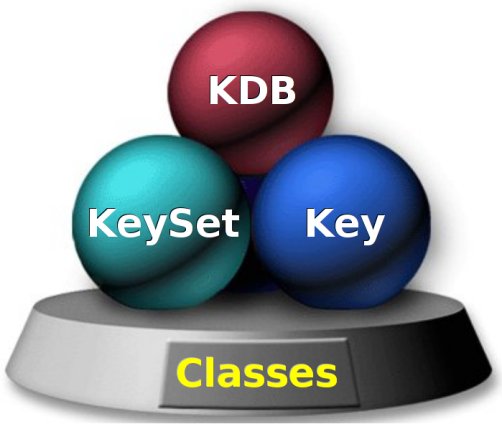
\includegraphics[height=\baselineskip,keepaspectratio=true]{classes.png}%Elektra Classes
\end{DoxyInlineImage}


Some general things you can do with each class are\+:

\mbox{\hyperlink{group__kdb}{KDB (Key Database)}}


\begin{DoxyItemize}
\item \mbox{\hyperlink{group__kdb_ga844e1299a84c3fbf1d3a905c5c893ba5}{Open}} and \mbox{\hyperlink{group__kdb_gadb54dc9fda17ee07deb9444df745c96f}{Close}} the Key Database
\item \mbox{\hyperlink{group__kdb_ga28e385fd9cb7ccfe0b2f1ed2f62453a1}{Get}} and \mbox{\hyperlink{group__kdb_ga11436b058408f83d303ca5e996832bcf}{Set}} \mbox{\hyperlink{group__keyset}{Key\+Set}} in the Key Database
\item See \mbox{\hyperlink{group__kdb}{class documentation}} for more
\end{DoxyItemize}

\mbox{\hyperlink{group__key}{Key}}


\begin{DoxyItemize}
\item \mbox{\hyperlink{group__key_gad23c65b44bf48d773759e1f9a4d43b89}{Create}} and \mbox{\hyperlink{group__key_ga3df95bbc2494e3e6703ece5639be5bb1}{Delete}}
\item Get and Set key the \mbox{\hyperlink{group__keyname_ga7699091610e7f3f43d2949514a4b35d9}{name}}
\item Get and Set \mbox{\hyperlink{group__keyvalue_ga622bde1eb0e0c4994728331326340ef2}{string}} or \mbox{\hyperlink{group__keyvalue_gaa50a5358fd328d373a45f395fa1b99e7}{binary}} values
\item Get and Set \mbox{\hyperlink{group__keymeta}{Metadata}}
\item See \mbox{\hyperlink{group__key}{class documentation}} for more
\end{DoxyItemize}

\mbox{\hyperlink{group__keyset}{Key\+Set}}


\begin{DoxyItemize}
\item \mbox{\hyperlink{group__keyset_ga671e1aaee3ae9dc13b4834a4ddbd2c3c}{Create}} and \mbox{\hyperlink{group__keyset_ga27e5c16473b02a422238c8d970db7ac8}{Delete}}
\item Append \mbox{\hyperlink{group__keyset_gaa5a1d467a4d71041edce68ea7748ce45}{a single key}} or an entire \mbox{\hyperlink{group__keyset_ga21eb9c3a14a604ee3a8bdc779232e7b7}{Key\+Set}}
\item \mbox{\hyperlink{group__keyset_ga60f1ddcf23272f2b29b90e92ebe9b56f}{Lookup keys}}
\item Pop \mbox{\hyperlink{group__keyset_gae42530b04defb772059de0600159cf69}{the last key}}, \mbox{\hyperlink{group__keyset_ga60f1ddcf23272f2b29b90e92ebe9b56f}{a key by name}}, or \mbox{\hyperlink{group__keyset_gaba1f1dbea191f4d7e7eb3e4296ae7d5e}{every key}}
\item Get a key at a \mbox{\hyperlink{group__keyset_gab3fb5e067c672d9fd60a4022b2ae9dd1}{specific position}}
\item Get the \mbox{\hyperlink{group__keyset_ga7474ad6b0a0fa969dbdf267ba5770eee}{number of elements}} in a Key\+Set
\item See \mbox{\hyperlink{group__keyset}{class documentation}} for more
\end{DoxyItemize}

\mbox{\hyperlink{doc_dev_classes_md}{More background information about the classes}}\hypertarget{index_autotoc_md685}{}\doxysection{Namespaces}\label{index_autotoc_md685}
There are 5 trees (=namespaces) of keys\+: {\ttfamily spec}, {\ttfamily proc}, {\ttfamily dir}, {\ttfamily user} and {\ttfamily system} that are all unified (in the given order) in one cascading tree starting with {\ttfamily /}.

The cascading tree is the logical tree to be used in applications. The other trees are the physical ones that stem from configuration sources. When using cascading key the best key will be searched at run-\/time, which appears like a tree on its own. See cascading in the documentation of \mbox{\hyperlink{group__keyset_gad65d2cdcbb5381194a1688e169af8a83}{ks\+Lookup\+By\+Name()}} on how the selection of keys works.


\begin{DoxyItemize}
\item The {\ttfamily spec} tree

This tree specifies how the lookup should take place and also allows us to define defaults or document a key. The metadata of a key contains this information\+:
\begin{DoxyItemize}
\item {\ttfamily override/\#}\+: use these keys {\itshape in favor} of the key itself (note that {\ttfamily \#} is the syntax for arrays, e.\+g. {\ttfamily \#0} for the first element, {\ttfamily \#10} for the 11th and so on)
\item {\ttfamily namespace/\#}\+: instead of using all namespaces in the predefined order, one can specify which namespaces should be searched in which order
\item {\ttfamily fallback/\#}\+: when no key was found in any of the (specified) namespaces the {\ttfamily fallback}-\/keys will be searched
\item {\ttfamily default}\+: this value will be used if nothing else was found
\end{DoxyItemize}
\item The {\ttfamily proc} tree

Is the only read-\/only tree. The configuration does not stem from the \mbox{\hyperlink{group__kdb}{KDB (Key Database)}}, but any other source, e.\+g. command-\/line arguments or environment.
\item The {\ttfamily dir} tree

Allows us to have a per-\/directory overwrite of configuration files, e.\+g. for project specific settings.
\item The {\ttfamily user} tree

Used to store user-\/specific configurations, like the personal settings of a user to certain programs. The user subtree will always be favored if present (except for security concerns the user subtree may not be considered).
\item The {\ttfamily system} tree

It is provided to store system-\/wide configuration keys, that is, the last fallback for applications but the only resort for daemons and system services.
\end{DoxyItemize}

Read more about \mbox{\hyperlink{doc_help_elektra-namespaces_md}{namespaces}} and a tutorial for \mbox{\hyperlink{doc_tutorials_namespaces_md}{namespaces}}.\hypertarget{index_autotoc_md686}{}\doxysection{Rules for Key Names}\label{index_autotoc_md686}
When using Elektra to store your application\textquotesingle{}s configuration and state, please keep in mind the following rules\+:


\begin{DoxyItemize}
\item You are not allowed to create keys right under the root. They are reserved for more generic purposes.
\item The keys for your application, called say {\itshape myapp}, should be created under {\ttfamily /sw/org/myapp/\#0/current}
\begin{DoxyItemize}
\item sw is for software
\item org is the organization. For uniqueness a full reverse url encoded with \textquotesingle{}/\textquotesingle{} instead of \textquotesingle{}.\textquotesingle{} is useful.
\item {\ttfamily \#0} is the major version of the configuration
\item current is the default configuration profile.
\item That means you just need to \mbox{\hyperlink{group__kdb_ga28e385fd9cb7ccfe0b2f1ed2f62453a1}{kdb\+Get()}} {\ttfamily /sw/org/myapp/\#0/profile} and then \mbox{\hyperlink{group__keyset_gad65d2cdcbb5381194a1688e169af8a83}{ks\+Lookup\+By\+Name()}} in {\ttfamily /sw/org/myapp/\#0/profile/key} where profile is from command-\/line arguments and defaults to current.
\end{DoxyItemize}
\end{DoxyItemize}

Read more about \mbox{\hyperlink{doc_help_elektra-key-names_md}{key names}}\hypertarget{index_autotoc_md687}{}\doxysection{Backend Overview}\label{index_autotoc_md687}
The core of Elektra does not store configuration itself to the hard disk. Instead this work is delegated to backends.

If you want to develop a backend, you should already have some experience with Elektra from the user point of view. You should be familiar with the data structures\+: \mbox{\hyperlink{group__key}{Key}} and \mbox{\hyperlink{group__keyset}{Key\+Set}} Then you can start reading about Backends that are composed out of \mbox{\hyperlink{group__plugin}{Plugins}}. To get started with writing plugins, first read our \mbox{\hyperlink{doc_tutorials_plugins_md}{plugin tutorial}} and then lookup details in the API description in \mbox{\hyperlink{group__plugin}{Plugins}}.

Read more about \mbox{\hyperlink{doc_help_elektra-mounting_md}{mounting}}\hypertarget{index_autotoc_md688}{}\doxysection{See Also}\label{index_autotoc_md688}

\begin{DoxyItemize}
\item See \mbox{\hyperlink{doc_help_elektra-glossary_md}{elektra-\/glossary(7)}}
\item More information about \mbox{\hyperlink{doc_help_elektra-backends_md}{elektra-\/backends(7)}}
\item More information about \mbox{\hyperlink{doc_dev_plugins-framework_md}{plugins-\/framework}} 
\end{DoxyItemize}
\chapter{R\+E\+A\+D\+M\+E}
\label{md_src_libs_getenv_README}
\hypertarget{md_src_libs_getenv_README}{}

\begin{DoxyItemize}
\item infos = Information about elektrify getenv below
\item infos/author = Markus Raab \href{mailto:elektra@libelektra.org}{\tt elektra@libelektra.\+org}
\item infos/description =
\end{DoxyItemize}

\section*{elektrify-\/getenv(1) -- elektrify the environment of applications }

{\ttfamily elektrify-\/getenv} $<$application$>$ $<$options$>$

\subsection*{E\+X\+A\+M\+P\+L\+E}

\begin{DoxyVerb}kdb elektrify-getenv curl --elektra-version
kdb elektrify-getenv curl http://www.libelektra.org
kdb set system/elektra/intercept/getenv/override/http_proxy http://www.example.com/
kdb elektrify-getenv curl http://www.libelektra.org
\end{DoxyVerb}


By using {\ttfamily elektrify-\/getenv} the last curl invocation will use a different http proxy. Or you can also reload while the application is running\+: \begin{DoxyVerb}ELEKTRA_RELOAD_TIMEOUT=100 kdb elektrify-getenv firefox
kdb set system/elektra/intercept/getenv/override/http_proxy http://www.example.com
\end{DoxyVerb}


\subsection*{D\+E\+S\+C\+R\+I\+P\+T\+I\+O\+N}

When an application is elektrified using libelektragetenv, it does not only request {\ttfamily environ}, but also Elektra for every getenv(3) and secure\+\_\+getenv(3) library call.

Its main purpose is to\+:


\begin{DoxyItemize}
\item have a standard ways to modify the environment
\item make relogin (or even restart!) of applications unnecessary
\item allow a hierarchical structure for environment
\item allow settings to only apply for individual applications or only in special context
\item still preserve the advantages (inheriting of environment to subprocesses)
\item availability of same environment in at, cron and similar scripts
\end{DoxyItemize}

It is implemented using a L\+D\+\_\+\+P\+R\+E\+L\+O\+A\+D technique, see \href{#USAGE}{\tt U\+S\+A\+G\+E} below for global activation.

\subsection*{L\+O\+O\+K\+U\+P\+S}

The main purpose of this approach is to finally have a well-\/defined way to set and get environment variables. Elektra's variables will be in use immediately for every newly started application (no relogin necessary).

To do so, getenv(3) will lookup multiple sources next to searching in the environment (environ). As running example will use {\ttfamily getenv(\char`\"{}\+H\+O\+M\+E\char`\"{}) -\/$>$ /path/to/home}\+:


\begin{DoxyEnumerate}
\item Given commandline parameters will always be preferred (see \href{#OPTIONS}{\tt O\+P\+T\+I\+O\+N\+S} below).

E.\+g. {\ttfamily elektrify-\/getenv $<$app$>$ -\/-\/elektra\+:H\+O\+M\+E=/path/to/home}
\item Then {\ttfamily /elektra/intercept/getenv/override/$<$key$>$} will be looked up, where $<$key$>$ is the parameter to {\ttfamily getenv}. If found, the key will be returned, if it is a null keys, {\ttfamily getenv} will return {\ttfamily N\+U\+L\+L}.

E.\+g. {\ttfamily kdb set user/elektra/intercept/getenv/override/\+H\+O\+M\+E /path/to/home}
\item Then environment will be requested.

E.\+g. {\ttfamily H\+O\+M\+E=/path/to/home elektrify-\/getenv $<$application$>$}
\item Then {\ttfamily /elektra/intercept/getenv/fallback/$<$key$>$} will be looked up. If found, the key will be returned, if it is a null keys, {\ttfamily getenv} will return {\ttfamily N\+U\+L\+L}.

E.\+g. {\ttfamily kdb set user/elektra/intercept/getenv/fallback/\+H\+O\+M\+E /path/to/home}
\end{DoxyEnumerate}

\subsection*{O\+P\+T\+I\+O\+N\+S}

When {\ttfamily elektrify-\/getenv} is active, every application additionally accepts Elektra's getenv options. Interleaving Elektra's and the application's options is allowed. Elektra will parse its options (starting with --elektra) first and discard them before the other application is started. Therefore the application will not see that they even existed, e.\+g.\+: given {\ttfamily elektrify-\/getenv $<$application$>$ -\/\+V -\/-\/elektra-\/debug -\/\+L} the application will be called with {\ttfamily $<$application$>$ -\/\+V -\/\+L}.

\subsubsection*{Internal Options}


\begin{DoxyItemize}
\item {\ttfamily -\/-\/elektra-\/help}\+: Outputs this help.
\item {\ttfamily -\/-\/elektra-\/version}\+: Gives version information.
\item {\ttfamily -\/-\/elektra-\/debug=file}, {\ttfamily E\+L\+E\+K\+T\+R\+A\+\_\+\+D\+E\+B\+U\+G} or {\ttfamily /elektra/intercept/getenv/option/debug}\+: Trace all getenv(3) calls to a file. stderr if no file is given, e.\+g. {\ttfamily kdb set user/elektra/intercept/getenv/option/debug \char`\"{}\char`\"{}}. Note that null values (no forth argument), will disable debug messages. See examples below.
\item {\ttfamily -\/-\/elektra-\/clearenv}, {\ttfamily E\+L\+E\+K\+T\+R\+A\+\_\+\+C\+L\+E\+A\+R\+E\+N\+V} or {\ttfamily /elektra/intercept/getenv/option/clearenv}\+: Call clearenv(3) before entering main. This is a recommended security feature. Elektra itself, if configured that way, will still be able to use the environment.
\item {\ttfamily -\/-\/elektra-\/reload-\/timeout=time\+\_\+in\+\_\+ms}, {\ttfamily E\+L\+E\+K\+T\+R\+A\+\_\+\+R\+E\+L\+O\+A\+D\+\_\+\+T\+I\+M\+E\+O\+U\+T} or {\ttfamily /elektra/intercept/getenv/option/reload\+\_\+timeout}\+: Activate a timeout based feature when a time is given in ms (and is not 0).
\end{DoxyItemize}

Internal Options are available in three different variants\+:


\begin{DoxyEnumerate}
\item as commandline parameter\+: {\ttfamily -\/-\/elektra-\/$<$option$>$}, which are {\itshape not} passed through exec(3) calls.
\item as environment variable\+: {\ttfamily E\+L\+E\+K\+T\+R\+A\+\_\+$<$O\+P\+T\+I\+O\+N$>$}. which might be passed through exec(3) calls, but are removed by clearenv(3) calls.
\item as Elektra K\+D\+B entry\+: {\ttfamily /elektra/intercept/getenv/option/$<$option$>$}, which are the way to achieve an option to be enabled for every application.

E.\+g. {\ttfamily kdb set user/elektra/intercept/getenv/option/clearenv \char`\"{}\char`\"{}} to clear the environment for all applications started by that user (note that at least {\ttfamily P\+A\+T\+H} should to be set using {\ttfamily kdb set user/elektra/intercept/getenv/fallback/\+P\+A\+T\+H \char`\"{}/bin\+:/usr/bin\char`\"{}} then).

Note, that null keys are equal to non-\/set options. E.\+g. {\ttfamily kdb set system/elektra/intercept/getenv/option/debug \char`\"{}/tmp/elektra.\+log\char`\"{}} and {\ttfamily kdb set user/elektra/intercept/getenv/option/debug} will activate logging for the system, except for the current user.
\end{DoxyEnumerate}

\subsubsection*{Contextual Options}


\begin{DoxyItemize}
\item {\ttfamily -\/-\/elektra\%$<$name$>$\%=$<$value$>$} or {\ttfamily /elektra/intercept/getenv/layer/$<$name$>$}\+: Add the contextual information (=layer) {\ttfamily \%$<$name$>$\%} with its value {\ttfamily $<$value$>$}. Note that {\ttfamily name\%} is predefined with {\ttfamily argv\mbox{[}0\mbox{]}} and {\ttfamily basename\%} with {\ttfamily basename(argv\mbox{[}0\mbox{]})}.
\end{DoxyItemize}

Values can contain / to form hierarchies, e.\+g. {\ttfamily -\/-\/elektraname\%=app/profile}

\subsubsection*{Options for Applications}


\begin{DoxyItemize}
\item {\ttfamily -\/-\/elektra\+:key=value}, {\ttfamily /elektra/intercept/getenv/override/$<$key$>$} or {\ttfamily /elektra/intercept/getenv/fallback/$<$key$>$}\+: set a key/value to be preferred, i.\+e. the first to considered as explained in \href{#LOOKUP}{\tt L\+O\+O\+K\+U\+P}.
\end{DoxyItemize}

Keys can contain / to form hierarchies, e.\+g. {\ttfamily -\/-\/elektra\+:my/\+H\+O\+M\+E=/path/to/home}.

\subsection*{U\+S\+A\+G\+E}

To always use Elektra's getenv environment, simply add the output to the file\+: \begin{DoxyVerb}elektrify-getenv | tail -1 | sudo tee -a /etc/ld.so.preload
\end{DoxyVerb}


this also can be done using Elektra\+: \begin{DoxyVerb}sudo kdb mount /etc/ld.so.preload system/ld/preload line null
sudo kdb set "system/ld/preload/new"  `elektrify-getenv | tail -1`
\end{DoxyVerb}


\subsection*{C\+O\+N\+T\+E\+X\+T}

The metadata {\ttfamily context} in the specification can be used to facilitate a context-\/dependent lookup. In its metavalue all replacements of {\ttfamily \%$<$name$>$\%} will be replaced by the given contextual options {\ttfamily -\/-\/elektra\%$<$name$>$\%=$<$value$>$} and {\ttfamily /elektra/intercept/getenv/layer/$<$name$>$} keys.

E.\+g. to have a different home directory for any user and application\+: \begin{DoxyVerb}kdb set user/elektra/intercept/getenv/layer/user markus
kdb set user/users/markus/konqueror/HOME /home/download
kdb setmeta spec/elektra/intercept/getenv/override/HOME context  /users/%user%/%name%/HOME
\end{DoxyVerb}


Or to have a different lock/suspend program per computer (that all have the same config)\+: \begin{DoxyVerb}kdb mount-info system/elektra/intercept/getenv/info            # must be below /elektra/intercept/getenv to be available
kdb setmeta spec/elektra/intercept/getenv/layer/hostname override/#0 system/elektra/intercept/getenv/info/uname/nodename
kdb setmeta spec/elektra/intercept/getenv/override/lock context /elektra/intercept/getenv/info/lock/%hostname%
kdb set user/elektra/intercept/getenv/info/lock/computer1 "systemctl suspend -i
kdb set user/elektra/intercept/getenv/info/lock/computer2 "xset dpms force off && xtrlock"
`kdb getenv lock`  # call the appropriate lock method for the current computer
\end{DoxyVerb}


\subsection*{B\+U\+G\+S}

Some applications do not use {\ttfamily getenv(3)} or {\ttfamily secure\+\_\+getenv(3)} for requesting the environment, e.\+g. shells. This approach cannot work for them.

In the startup-\/phase (before main is even entered), {\ttfamily getenv(3)} will not consider {\ttfamily /elektra/intercept/getenv/override/} or {\ttfamily /elektra/intercept/getenv/fallback}.

Elektra internally tries to avoid using the environment. Some resolvers, however, use it to conform to some specifications, e.\+g. X\+D\+G. Depending on the setup you use, these parameters might be used. For more information see\+: \begin{DoxyVerb}kdb info resolver
\end{DoxyVerb}


For these parameters, {\ttfamily /elektra/intercept/getenv/override/} or {\ttfamily /elektra/intercept/getenv/fallback} will {\itshape not} be used internally, but will be used if applications request them, too.

If you use the standard resolvers, the bug won't have any effect.

Also note that {\ttfamily -\/-\/elektra-\/debug} or {\ttfamily E\+L\+E\+K\+T\+R\+A\+\_\+\+D\+E\+B\+U\+G} does {\itshape not} log {\ttfamily getenv(3)} used by plugins during the startup-\/phase.

Command line arguments apply always to the outmost command, e.\+g. {\ttfamily nice ls -\/-\/elektra\+:C\+O\+L\+U\+M\+N\+S=20} won't have any effect because only for {\ttfamily nice} {\ttfamily C\+O\+L\+U\+M\+N\+S} will be set.

\subsection*{E\+X\+A\+M\+P\+L\+E\+S}

For illustration this section gives some more examples. \begin{DoxyVerb}elektrify-getenv man man --elektra:MANWIDTH=40
\end{DoxyVerb}


Will use M\+A\+N\+W\+I\+D\+T\+H 40 for this invocation of man man. This feature is handy, if an option is only available by environment, but not by command-\/line arguments, because sometimes environment variables are not trivial to set (e.\+g. in Makefiles).

Debugging\+: \begin{DoxyVerb}# system wide to stderr (not recommended!):
sudo kdb set system/elektra/intercept/getenv/option/debug ""
# system wide to /var/log/elektra.log:
sudo kdb set system/elektra/intercept/getenv/option/debug "/var/log/error.log"
# but for my user to ~/.elektra.log:
kdb set user/elektra/intercept/getenv/option/debug "$HOME/.elektra.log"
# or disable it for my user:
kdb set user/elektra/intercept/getenv/option/debug
\end{DoxyVerb}


Some more examples\+: \begin{DoxyVerb}kdb set user/elektra/intercept/getenv/override/MANOPT -- "--regex -LC"
elektrify-getenv getenv MANOPT   # to check if it is set as expected
kdb getenv MANOPT   # if /etc/ld.so.preload is active
\end{DoxyVerb}


Will permanently and user-\/wide change M\+A\+N\+O\+P\+T to include --regex, and -\/\+L\+C so that regular expressions will be used (note {\ttfamily man echo} will return many man pages then) and that they will be shown in English. This feature is handy to change the default behaviour of applications (either system, user or directory-\/wide).

\begin{DoxyVerb}kdb set system/elektra/intercept/getenv/override/HTTP_PROXY http://proxy.hogege.com:8000/
\end{DoxyVerb}


Will permanently and system-\/wide change the proxy for all applications that honor H\+T\+T\+P\+\_\+\+P\+R\+O\+X\+Y, e.\+g. w3m. We can also link {\ttfamily http\+\_\+proxy} to the value of {\ttfamily H\+T\+T\+P\+\_\+\+P\+R\+O\+X\+Y}\+: \begin{DoxyVerb}kdb setmeta spec/elektra/intercept/getenv/override/http_proxy "override/#0" /elektra/intercept/getenv/override/HTTP_PROXY
kdb get /elektra/intercept/getenv/override/http_proxy\end{DoxyVerb}
 
\chapter{elektra-\/libs(7) -\/-\/ libs overview}
\label{md_src_libs_README}
\hypertarget{md_src_libs_README}{}
Since \hyperlink{doc_decisions_library_split_md}{0.8.15} libelektra is split in following libraries\+:



\subsection*{Loader}

loader contains source files that implement the plugin loader functionality. The files are linked to libelektra.

\subsection*{Libease}

\begin{DoxyVerb}libelektra-ease.so
\end{DoxyVerb}


libease contains data-\/structure operations on top of libcore which do not depend on internals. Applications and plugins can choose to not link against it if they want to stay minimal.

\subsection*{Libplugin}

\begin{DoxyVerb}libelektra-plugin.so
\end{DoxyVerb}


libplugin contains elektra\+Plugin$\ast$ symbols and plugins should link against it.

\subsection*{Libproposal}

\begin{DoxyVerb}libelektra-proposal.so
\end{DoxyVerb}


libproposal contains functions that are proposed for libcore. Depends on internas of libcore and as such must always fit to the exact same version.

\subsection*{Libmeta}

\begin{DoxyVerb}libelektra-meta.so
\end{DoxyVerb}


\href{/home/markus/Projekte/Elektra/current/src/libs/meta/meta.c}{\tt libmeta} contains meta data operations as described in \href{/home/markus/Projekte/Elektra/current/doc/METADATA.ini}{\tt M\+E\+T\+A\+D\+A\+T\+A.\+ini}. Will be code-\/generated in the future, so methods should be mechanical reflections of the contents in \href{/home/markus/Projekte/Elektra/current/doc/METADATA.ini}{\tt M\+E\+T\+A\+D\+A\+T\+A.\+ini}.

\subsection*{Libcore}

\begin{DoxyVerb}libelektra-core.so
<kdbhelper.h>
<kdb.h> (key* and ks*)
\end{DoxyVerb}


Contains the fundamental data-\/structures every participant of Elektra needs to link against. It should be the only part that access the internal data structures.

\subsection*{Libtools}

libtools is a high-\/level C++ shared-\/code for tools. It includes\+:


\begin{DoxyItemize}
\item plugin interface
\item backend interface
\item 3-\/way merge 
\end{DoxyItemize}
\chapter{Plugin\+: augeas}
\label{md_src_plugins_augeas_README}
\hypertarget{md_src_plugins_augeas_README}{}

\begin{DoxyItemize}
\item infos = Information about augeas plugin is in keys below
\item infos/author = Felix Berlakovich \href{mailto:elektra@berlakovich.net}{\tt elektra@berlakovich.\+net}
\item infos/licence = B\+S\+D
\item infos/provides = storage
\item infos/needs =
\item infos/recommends = glob keytometa
\item infos/placements = getstorage setstorage
\item infos/status = maintained unittest libc configurable
\item infos/description = reading and writing configurations via libaugeas
\end{DoxyItemize}

This is a plugin for reading and writing configuration files with help from Augeas. The plugin should be able to read all configuration files for which an Augeas lens exists. However, not all stock lenses of Augeas have been tested yet. A detailed description of the lens language and a tutorial on how to write new lenses can be found at \href{http://augeas.net/}{\tt http\+://augeas.\+net/}

\subsection*{Dependencies}


\begin{DoxyItemize}
\item {\ttfamily libaugeas-\/dev}\+: You need version 0.\+16 or higher
\end{DoxyItemize}

\subsection*{Installation}

If you have installed Augeas manually, it may be necessary to update the ld configuration. This is especially true if an older version of Augeas is installed also. Such a situation may lead to an error similar to this\+: \begin{DoxyVerb}/usr/lib/libaugeas.so.0: version `AUGEAS_0.16.0` not found (required by kdb)
\end{DoxyVerb}


This is because {\ttfamily ld} tries to link {\ttfamily /usr/lib/libaugeas.so.\+0} which is an older version of Augeas. Simply add the path to the newer library to your ld search paths (consult your system documentation on how to do this).

\subsection*{Mounting and Configuration}

In order to mount the hosts file with the augeas plugin, issue the following command\+: \begin{DoxyVerb}kdb mount /etc/hosts system/hosts augeas lens=Hosts.lns
\end{DoxyVerb}


The value of the plugin configuration option \char`\"{}lens\char`\"{} should be the module name of the lens (Hosts in the example) with a '.lns' suffix. Depending on your distribution and kind of installation, lenses can be found at {\ttfamily /usr/share/augeas/lenses/dist}, {\ttfamily /usr/local/share/augeas/lenses/dist}, or something similar. The lens module name is equal to the filename without extension in pascal notation. For example, the lens {\ttfamily /usr/share/augeas/lenses/dist/hosts.aug} contains the module Hosts.

Note that, without configuring the plugin to use a lens, the plugin will print an error message on the first usage\+: \begin{DoxyVerb}kdb ls system/hosts
The command ls terminated unsuccessfully with the info: Error (#85) occurred!
Description: an Augeas error occurred
Ingroup: plugin
Module: storage
At: /path/augeas.c:166
Reason: Lens not found
\end{DoxyVerb}


This happens because the plugin does not know which lens it should use to read and write the configuration. For that reason, the lens configuration option was supplied together with the mount command.

\subsection*{Restrictions}

\subsubsection*{Inner node values}

Currently no Augeas lens supports values for inner nodes. Unfortunately no validation plugin exists yet that would prevent such modifications early\+: \begin{DoxyVerb}kdb set system/hosts/1 somevalue
The command set terminated unsuccessfully with the info: Error (#85) occurred!
Description: an Augeas error occurred
Ingroup: plugin
Module: storage
At: /path/augeas.c:166
Reason: Malformed child node '1'
\end{DoxyVerb}


The operation simply fails with an undescriptive error.

\subsubsection*{Leaky abstraction of order}

Most Augeas lenses require subtrees to be in a specific order. For example the hosts lens requires the ipaddr node of an entry to precede the canonical node. Unfortunately the Augeas storage plugin has no knowledge about this required order. Therefore the correct order must be ensured via order metakeys. Otherwise saving the Key\+Set may fail. As an example consider the following kdb shell script\+: \begin{DoxyVerb}kdbGet system/hosts
keySetName system/hosts/6
ksAppendKey
keySetName system/hosts/6/ipaddr
keySetString 14.14.14.14
ksAppendKey
keySetName system/hosts/6/canonical
keySetString newhost
ksAppendKey
kdbSet system/hosts
\end{DoxyVerb}


This fails with an error similar to this \begin{DoxyVerb}Description: an Augeas error occurred
Ingroup: plugin
Module: storage
At: /path/augeas.c:179
Reason: Failed to match
some augeas match expression
with tree
{ \"canonical\" = \"newhost\" } { \"ipaddr\" = \"14.14.14.14\" }
\end{DoxyVerb}


Wheras the following script succeeds due to the correct order \begin{DoxyVerb}kdbGet system/hosts
keySetName system/hosts/6
ksAppendKey
keySetName system/hosts/6/ipaddr
keySetString 14.14.14.14
keySetMeta order 100
ksAppendKey
keySetName system/hosts/6/canonical
keySetString newhost
keySetMeta order 110
ksAppendKey
kdbSet system/hosts
\end{DoxyVerb}


\subsection*{Planned Improvements}


\begin{DoxyItemize}
\item a validation plugin preventing inner node values 
\end{DoxyItemize}
\chapter{Plugin\+: ccode}
\label{md_src_plugins_ccode_README}
\hypertarget{md_src_plugins_ccode_README}{}

\begin{DoxyItemize}
\item infos = Information about ccode plugin is in keys below
\item infos/author = Markus Raab \href{mailto:elektra@libelektra.org}{\texttt{ elektra@libelektra.\+org}}
\item infos/licence = BSD
\item infos/provides = code
\item infos/needs =
\item infos/recommends =
\item infos/placements = postgetstorage presetstorage
\item infos/status = unittest nodep libc configurable discouraged
\item infos/description = Decoding/\+Encoding engine which escapes unwanted characters.
\end{DoxyItemize}\hypertarget{md_src_plugins_ccode_README_src_plugins_ccode_README_md}{}\doxysection{CCode}\label{md_src_plugins_ccode_README_src_plugins_ccode_README_md}
\hypertarget{md_src_plugins_ccode_README_autotoc_md80}{}\doxysubsection{Introduction}\label{md_src_plugins_ccode_README_autotoc_md80}
The {\ttfamily ccode} plugin replaces (escapes) any special characters with two characters\+:


\begin{DoxyItemize}
\item an escape character (default\+: {\ttfamily \textbackslash{}}) and
\item another character representing the escaped character (e.\+g {\ttfamily n} for newline)
\end{DoxyItemize}

before writing a {\ttfamily Key\+Set}. The plugin undoes this modification after reading a {\ttfamily Key\+Set}.

CCode provides a reasonable default configuration, using the usual escape sequences for C strings (e.\+g. {\ttfamily \textbackslash{}n} for newline, {\ttfamily \textbackslash{}t} for tab). You can also configure the escape character ({\ttfamily /escape}) and the mapping for special characters ({\ttfamily chars}).\hypertarget{md_src_plugins_ccode_README_autotoc_md81}{}\doxysubsection{Installation}\label{md_src_plugins_ccode_README_autotoc_md81}
See \mbox{\hyperlink{doc_INSTALL_md}{installation}}. The package is called {\ttfamily libelektra5-\/extra}.\hypertarget{md_src_plugins_ccode_README_autotoc_md82}{}\doxysubsection{Restrictions}\label{md_src_plugins_ccode_README_autotoc_md82}
This method of encoding characters is not as powerful as the hexcode plugin in terms of reduction. The hexcode plugin allows reduction of the character set to \textquotesingle{}0\textquotesingle{}-\/\textquotesingle{}9\textquotesingle{}, \textquotesingle{}a\textquotesingle{}-\/\textquotesingle{}f\textquotesingle{} and one escape character. So it can represent any key value with only 17 characters. On the other hand, ccode cannot reduce the set more than by half.

So when all control characters and non-\/\+ASCII characters need to vanish, it cannot be done with the ccode plugin. But it is perfectly suitable to reduce by some characters. The advantages are that the size only doubles in the worst case and that it is much easier to read.\hypertarget{md_src_plugins_ccode_README_autotoc_md83}{}\doxysubsection{C}\label{md_src_plugins_ccode_README_autotoc_md83}
In the C language, the following escape characters are present.


\begin{DoxyItemize}
\item {\ttfamily b}\+: backspace, hex\+: 08
\item {\ttfamily t}\+: horizontal tab, hex\+: 09
\item {\ttfamily n}\+: new line feed, hex\+: 0A
\item {\ttfamily v}\+: vertical tab, hex\+: 0B
\item {\ttfamily f}\+: form feed, hex\+: 0C
\item {\ttfamily r}\+: carriage return, hex\+: 0D
\item {\ttfamily \textbackslash{}\textbackslash{}}\+: back slash, hex\+: 5C
\item `'{\ttfamily \+: single quote, hex\+: 27 -\/}"{}{\ttfamily \+: double quote, hex\+: 22 -\/}0\`{}\+: null, hex\+: 00
\end{DoxyItemize}

This is also the default mapping.\hypertarget{md_src_plugins_ccode_README_autotoc_md84}{}\doxysubsubsection{Contract}\label{md_src_plugins_ccode_README_autotoc_md84}
Add {\ttfamily ccode} to {\ttfamily infos/needs} for any plugin that you want to be filtered by ccode. 
\chapter{Plugin\+: conditionals}
\label{md_src_plugins_conditionals_README}
\hypertarget{md_src_plugins_conditionals_README}{}

\begin{DoxyItemize}
\item infos = Information about the conditionals plugin is in keys below
\item infos/author = Thomas Waser \href{mailto:thomas.waser@libelektra.org}{\texttt{ thomas.\+waser@libelektra.\+org}}
\item infos/licence = BSD
\item infos/provides =
\item infos/needs =
\item infos/recommends =
\item infos/placements = postgetstorage presetstorage
\item infos/status = unittest nodep libc global preview
\item infos/metadata = check/condition assign/condition condition/validsuffix check/condition/any/\# check/condition/all/\# check/condition/none/\# assign/condition/\#
\item infos/description = ensures key values through conditions
\end{DoxyItemize}\hypertarget{md_src_plugins_conditionals_README_src_plugins_conditionals_README_md}{}\doxysection{Introduction}\label{md_src_plugins_conditionals_README_src_plugins_conditionals_README_md}
This plugin uses if-\/then-\/else like conditions. It also works as global plugin.\hypertarget{md_src_plugins_conditionals_README_autotoc_md105}{}\doxysection{Installation}\label{md_src_plugins_conditionals_README_autotoc_md105}
See \mbox{\hyperlink{doc_INSTALL_md}{installation}}. The package is called {\ttfamily libelektra5-\/extra}.\hypertarget{md_src_plugins_conditionals_README_autotoc_md106}{}\doxysection{Check Syntax}\label{md_src_plugins_conditionals_README_autotoc_md106}
Stored in the metakey {\ttfamily check/condition} to validate data is\+:

{\ttfamily (IF-\/condition) ? (THEN-\/condition) \+: (ELSE-\/condition)} where the ELSE-\/condition is optional

Condition\+: {\ttfamily Key} {\itshape Operation} `(\textquotesingle{}String' $\vert$ \textquotesingle{}1234.\+56\textquotesingle{} $\vert$ Key $\vert$ \textquotesingle{}\textquotesingle{})\`{}

Operations\+: {\ttfamily !=, ==, $<$, $<$=, =$>$, $>$, \+:=}, where\+:


\begin{DoxyItemize}
\item {\ttfamily \+:=} is used to set a key value
\item others are for comparison as in C
\end{DoxyItemize}\hypertarget{md_src_plugins_conditionals_README_autotoc_md107}{}\doxysubsection{Testing if Key Exists}\label{md_src_plugins_conditionals_README_autotoc_md107}
{\ttfamily (! a/key)} evaluates to true if the key {\ttfamily a/key} doesn\textquotesingle{}t exist, to false if it exists.\hypertarget{md_src_plugins_conditionals_README_autotoc_md108}{}\doxysubsection{Assign Syntax}\label{md_src_plugins_conditionals_README_autotoc_md108}

\begin{DoxyCode}{0}
\DoxyCodeLine{(IF-\/condition) ? ('ThenValue') : ('ElseValue')}

\end{DoxyCode}


Depending on if the condition is met, either \textquotesingle{}Then\+Value\textquotesingle{} or \textquotesingle{}Else\+Value\textquotesingle{} will be assigned as key value if the metakey {\ttfamily assign/condition} is used.\hypertarget{md_src_plugins_conditionals_README_autotoc_md109}{}\doxysubsection{Experimental\+: Nested Conditions}\label{md_src_plugins_conditionals_README_autotoc_md109}
Multiple conditions can be nested and combined using parentheses and {\ttfamily \&\&} (logical AND) or {\ttfamily $\vert$$\vert$} (logical OR). Additional parentheses must be used to form valid conditions again. {\ttfamily (} {\ttfamily (condition 1) \&\& (condition 2)} {\ttfamily )}\hypertarget{md_src_plugins_conditionals_README_autotoc_md110}{}\doxysubsection{Valid Suffix}\label{md_src_plugins_conditionals_README_autotoc_md110}
The {\ttfamily condition/validsuffix} can be used to define a list of valid suffixes to numeric values. If two operants have the same valid suffix or one of them no suffix they will be treated by their numeric value ignoring their suffix. `condition/validsuffix = \textquotesingle{}m', \textquotesingle{}cm\textquotesingle{}, \textquotesingle{}km\textquotesingle{}{\ttfamily would treat}2.\+3m{\ttfamily just as the numeric value}2.\+3\`{} when comparing to another value having the same or no suffix.\hypertarget{md_src_plugins_conditionals_README_autotoc_md111}{}\doxysubsection{Keynames}\label{md_src_plugins_conditionals_README_autotoc_md111}
Keynames are all either relative to to-\/be-\/tested key (starting with {\ttfamily ./} or {\ttfamily ../}), relative to the parentkey (starting with {\ttfamily @/}) or absolute (e.\+g. {\ttfamily system\+:/key}).\hypertarget{md_src_plugins_conditionals_README_autotoc_md112}{}\doxysubsection{Multiple Statements}\label{md_src_plugins_conditionals_README_autotoc_md112}
It\textquotesingle{}s also possible to test multiple conditions using {\ttfamily check/condition/\{any,all,none\}} as a meta array. Where {\ttfamily any} means that at least one statement has to evaluate to true, {\ttfamily all} that all statements have to evaluate to true, and {\ttfamily none} that no statement is allowed to evaluate to false (default). For multiple assign statements use {\ttfamily assign/condition} as a meta array. The first {\ttfamily assign/condition/\#} statement that evaluates to true will be assigned and the rest ignored.\hypertarget{md_src_plugins_conditionals_README_autotoc_md113}{}\doxysection{Example}\label{md_src_plugins_conditionals_README_autotoc_md113}

\begin{DoxyCode}{0}
\DoxyCodeLine{(this/key  != 'value') ? (then/key == some/other/key) : (or/key <= '125')}

\end{DoxyCode}


Meaning\+: IF {\ttfamily this/key} NOT EQUAL TO `\textquotesingle{}value'{\ttfamily THEN}then/key{\ttfamily MUST EQUAL}some/other/key{\ttfamily ELSE}or/key{\ttfamily MUST BE LESS THAN}125\`{}

Another full example\+:


\begin{DoxyCode}{0}
\DoxyCodeLine{\#Backup-\/and-\/Restore:user:/tests/conditionals}
\DoxyCodeLine{}
\DoxyCodeLine{sudo kdb mount conditionals.dump user:/tests/conditionals conditionals dump}
\DoxyCodeLine{}
\DoxyCodeLine{kdb set user:/tests/conditionals/fkey 3.0}
\DoxyCodeLine{kdb set user:/tests/conditionals/hkey hello}
\DoxyCodeLine{}
\DoxyCodeLine{\# will succeed}
\DoxyCodeLine{kdb meta-\/set user:/tests/conditionals/key check/condition "{}(../hkey == 'hello') ? (../fkey == '3.0')"{}}
\DoxyCodeLine{}
\DoxyCodeLine{\# will fail}
\DoxyCodeLine{kdb meta-\/set user:/tests/conditionals/key check/condition "{}(../hkey == 'hello') ? (../fkey == '5.0')"{}}
\DoxyCodeLine{\# RET:5}
\DoxyCodeLine{\# ERROR:C03200}

\end{DoxyCode}


Assignment example\+:


\begin{DoxyCode}{0}
\DoxyCodeLine{kdb set user:/tests/conditionals/hkey Hello}
\DoxyCodeLine{kdb meta-\/set user:/tests/conditionals/hkey assign/condition "{}(./ == 'Hello') ? ('World')"{}}
\DoxyCodeLine{\# alternative syntax: "{}(../hkey == 'Hello') ? ('World')}
\DoxyCodeLine{}
\DoxyCodeLine{kdb get user:/tests/conditionals/hkey}
\DoxyCodeLine{\#> World}
\DoxyCodeLine{}
\DoxyCodeLine{\# cleanup}
\DoxyCodeLine{kdb rm -\/r user:/tests/conditionals}
\DoxyCodeLine{sudo kdb umount user:/tests/conditionals}

\end{DoxyCode}


Global plugin example\+:


\begin{DoxyCode}{0}
\DoxyCodeLine{\# Backup old list of global plugins}
\DoxyCodeLine{kdb set user:/tests/msr \$(mktemp)}
\DoxyCodeLine{kdb export system:/elektra/globalplugins > \$(kdb get user:/tests/msr)}
\DoxyCodeLine{}
\DoxyCodeLine{sudo kdb mount main.ini /tests/conditionals ni}
\DoxyCodeLine{sudo kdb mount sub.ini /tests/conditionals/sub ni}
\DoxyCodeLine{}
\DoxyCodeLine{\# mount conditionals as global plugin}
\DoxyCodeLine{sudo kdb global-\/mount conditionals || \$(exit 0)}
\DoxyCodeLine{}
\DoxyCodeLine{\# create testfiles}
\DoxyCodeLine{echo 'key1=val1'                                               >  `kdb file system:/tests/conditionals`}
\DoxyCodeLine{echo '[key1]'                                                    >> `kdb file system:/tests/conditionals`}
\DoxyCodeLine{echo "{}check/condition=(./ == 'val1') ? (../sub/key == 'true')"{} >> `kdb file system:/tests/conditionals`}
\DoxyCodeLine{}
\DoxyCodeLine{echo "{}key=false"{} > `kdb file system:/tests/conditionals/sub`}
\DoxyCodeLine{}
\DoxyCodeLine{\# should fail and yield an error}
\DoxyCodeLine{kdb export system:/tests/conditionals ni}
\DoxyCodeLine{\# ERROR:C03200}
\DoxyCodeLine{\# Sorry, module conditionals issued the error C03200:}
\DoxyCodeLine{\# Validation failed: Validation of Key key1: (./ == 'val1') ? (../sub/key == 'true') failed. ((../sub/key == 'true') failed)}
\DoxyCodeLine{}
\DoxyCodeLine{kdb set system:/tests/conditionals/sub/key true}
\DoxyCodeLine{}
\DoxyCodeLine{\# should succeed}
\DoxyCodeLine{kdb export system:/tests/conditionals ni}
\DoxyCodeLine{}
\DoxyCodeLine{\# cleanup}
\DoxyCodeLine{kdb rm -\/r /tests/conditionals}
\DoxyCodeLine{sudo kdb umount /tests/conditionals/sub}
\DoxyCodeLine{sudo kdb umount /tests/conditionals}
\DoxyCodeLine{}
\DoxyCodeLine{sudo kdb global-\/umount conditionals}
\DoxyCodeLine{}
\DoxyCodeLine{kdb rm -\/r system:/elektra/globalplugins}
\DoxyCodeLine{kdb import system:/elektra/globalplugins < \$(kdb get user:/tests/msr)}
\DoxyCodeLine{rm \$(kdb get user:/tests/msr)}
\DoxyCodeLine{kdb rm user:/tests/msr}

\end{DoxyCode}
 
\chapter{Plugin\+: constants}
\label{md_src_plugins_constants_README}
\hypertarget{md_src_plugins_constants_README}{}

\begin{DoxyItemize}
\item infos = All information you want to know
\item infos/author = Markus Raab \href{mailto:elektra@libelektra.org}{\tt elektra@libelektra.\+org}
\item infos/licence = B\+S\+D
\item infos/provides = storage
\item infos/placements = setstorage getstorage
\item infos/needs =
\item infos/recommends =
\item infos/description = Includes constants information into the key database.
\end{DoxyItemize}

The plugin is readonly.

To mount it, use \begin{DoxyVerb}    kdb mount -R noresolver none system/constants constants
\end{DoxyVerb}


To list all constants, use\+: \begin{DoxyVerb}    kdb ls system/constants\end{DoxyVerb}
 
\chapter{Plugin\+: counter}
\label{md_src_plugins_counter_README}
\hypertarget{md_src_plugins_counter_README}{}

\begin{DoxyItemize}
\item infos = Information about the counter plugin is in keys below
\item infos/author = Markus Raab \href{mailto:elektra@libelektra.org}{\tt elektra@libelektra.\+org}
\item infos/licence = B\+SD
\item infos/provides = tracing
\item infos/needs =
\item infos/recommends =
\item infos/placements = pregetstorage
\item infos/status = maintained nodep configurable final global nodoc
\item infos/metadata =
\item infos/description = counts and prints usage statistics
\end{DoxyItemize}

Counts and prints usage statistics. Only useful for debugging the plugin framework.

\subsection*{Module Loading}

Will not log when loaded as module (config {\ttfamily /module} present), unless {\ttfamily /logmodule} is set\+:


\begin{DoxyCode}
kdb check -c "logmodule=" counter
\end{DoxyCode}
 
\chapter{Plugin\+: crypto}
\label{md_src_plugins_crypto_README}
\hypertarget{md_src_plugins_crypto_README}{}

\begin{DoxyItemize}
\item infos = Information about crypto plugin is in keys below
\item infos/author = Peter Nirschl \href{mailto:peter.nirschl@gmail.com}{\texttt{ peter.\+nirschl@gmail.\+com}}
\item infos/licence = B\+SD
\item infos/provides = crypto
\item infos/needs =
\item infos/recommends =
\item infos/placements = postgetstorage presetstorage
\item infos/status = unittest configurable memleak unfinished discouraged
\item infos/metadata = crypto/encrypt
\item infos/description = Cryptographic operations
\end{DoxyItemize}\hypertarget{md_src_plugins_crypto_README_src_plugins_crypto_README_md}{}\doxysection{Introduction}\label{md_src_plugins_crypto_README_src_plugins_crypto_README_md}
This plugin is a filter plugin allowing Elektra to encrypt values before they are persisted and to decrypt values after they have been read from a backend.

The idea is to provide protection of sensible values before they are persisted. This means the value of a key needs to be encrypted before it is written to a file or a database. It also needs to be decrypted whenever an admissible access (read) is being performed.

The users of Elektra should not be bothered too much with the internals of the cryptographic operations. Also the cryptographic keys must never be exposed to the outside of the crypto module.

The crypto plugin uses libgcrypt as provider of cryptographic operations.\hypertarget{md_src_plugins_crypto_README_autotoc_md112}{}\doxysection{Dependencies}\label{md_src_plugins_crypto_README_autotoc_md112}

\begin{DoxyItemize}
\item {\ttfamily libgcrypt20-\/dev} or {\ttfamily libgcrypt-\/devel}
\end{DoxyItemize}\hypertarget{md_src_plugins_crypto_README_autotoc_md113}{}\doxysubsection{Gnu\+P\+G (\+G\+P\+G)}\label{md_src_plugins_crypto_README_autotoc_md113}
G\+PG is a run-\/time dependency of the crypto plugin. Either the {\ttfamily gpg} or the {\ttfamily gpg2} binary must be installed when using the plugin. Note that {\ttfamily gpg2} will be preferred if both versions are available. The G\+PG binary can be configured in the plugin configuration as {\ttfamily /gpg/bin} (see {\itshape G\+PG Configuration} below). If no such configuration is provided, the plugin will look at the P\+A\+TH environment variable to find the G\+PG binaries.\hypertarget{md_src_plugins_crypto_README_autotoc_md114}{}\doxysection{How to compile}\label{md_src_plugins_crypto_README_autotoc_md114}
Add \char`\"{}crypto\char`\"{} to the {\ttfamily P\+L\+U\+G\+I\+NS} variable in {\ttfamily C\+Make\+Cache.\+txt} and re-\/run {\ttfamily cmake}.

An example {\ttfamily C\+Make\+Cache.\+txt} may contain the following variable\+:


\begin{DoxyCode}{0}
\DoxyCodeLine{PLUGINS=crypto}
\end{DoxyCode}
\hypertarget{md_src_plugins_crypto_README_autotoc_md115}{}\doxysubsection{mac\+OS}\label{md_src_plugins_crypto_README_autotoc_md115}
The crypto plugin works under mac\+OS Sierra (Version 10.\+12.\+3 (16D32)).

To set up the build environment on mac\+OS Sierra we recommend using \href{http://brew.sh/}{\texttt{ Homebrew}}. Follow these steps to get everything up and running\+:


\begin{DoxyCode}{0}
\DoxyCodeLine{brew install libgcrypt pkg-\/config cmake}
\end{DoxyCode}


Also a G\+PG installation is required. The \href{https://gpgtools.org}{\texttt{ G\+PG Tools}} work fine for us.\hypertarget{md_src_plugins_crypto_README_autotoc_md116}{}\doxysection{Restrictions}\label{md_src_plugins_crypto_README_autotoc_md116}
At the moment the plugin will only run on Unix/\+Linux-\/like systems, that provide implementations for {\ttfamily fork ()} and {\ttfamily execv ()}.\hypertarget{md_src_plugins_crypto_README_autotoc_md117}{}\doxysection{Examples}\label{md_src_plugins_crypto_README_autotoc_md117}
To mount a backend with the crypto plugin that uses the G\+PG key 9C\+C\+C3\+B514\+E196\+C6308\+C\+C\+D230666260\+C14\+A525406, use\+:


\begin{DoxyCode}{0}
\DoxyCodeLine{kdb mount test.ecf user/t crypto "crypto/key=9CCC3B514E196C6308CCD230666260C14A525406"}
\end{DoxyCode}


Now you can specify a key {\ttfamily user/t/a} and protect its content by using\+:


\begin{DoxyCode}{0}
\DoxyCodeLine{kdb set user/t/a}
\DoxyCodeLine{kdb meta-\/set user/t/a crypto/encrypt 1}
\DoxyCodeLine{kdb set user/t/a "secret"}
\end{DoxyCode}


The value of {\ttfamily user/t/a} will be stored encrypted. But you can still access the original value using {\ttfamily kdb get}\+:


\begin{DoxyCode}{0}
\DoxyCodeLine{kdb get user/t/a}
\end{DoxyCode}
\hypertarget{md_src_plugins_crypto_README_autotoc_md118}{}\doxysection{Configuration}\label{md_src_plugins_crypto_README_autotoc_md118}
\hypertarget{md_src_plugins_crypto_README_autotoc_md119}{}\doxysubsection{G\+P\+G Configuration}\label{md_src_plugins_crypto_README_autotoc_md119}
The path to the gpg binary can be specified in


\begin{DoxyCode}{0}
\DoxyCodeLine{/gpg/bin}
\end{DoxyCode}


The G\+PG recipient keys can be specified as {\ttfamily encrypt/key} directly. If you want to use more than one key, just enumerate like\+:


\begin{DoxyCode}{0}
\DoxyCodeLine{encrypt/key/\#0}
\DoxyCodeLine{encrypt/key/\#1}
\end{DoxyCode}


If more than one key is defined, every owner of the corresponding private key can decrypt the values of the backend. This might be useful if applications run with their own user but the administrator has to update the configuration. The administrator then only needs the public key of the application user in her keyring, set the values and the application will be able to decrypt the values.

If you are not sure which keys are available to you, the {\ttfamily kdb} program will give you suggestions in the error description. For example you can type\+:


\begin{DoxyCode}{0}
\DoxyCodeLine{kdb mount test.ecf user/t crypto}
\end{DoxyCode}


In the error description you should see something like\+:


\begin{DoxyCode}{0}
\DoxyCodeLine{The command ./bin/kdb mount terminated unsuccessfully with the info:}
\DoxyCodeLine{The provided plugin configuration is not valid!}
\DoxyCodeLine{Errors/Warnings during the check were:}
\DoxyCodeLine{Sorry, module crypto issued the error C01310:}
\DoxyCodeLine{Failed to create handle. Reason: Missing GPG key (specified as encrypt/key) in plugin configuration. Available key IDs are: B815F1334CF4F830187A784256CFA3A5C54DF8E4,847378ABCF0A552B48082A80C52E8E92F785163F}
\DoxyCodeLine{Please report the issue at https://issues.libelektra.org/}
\end{DoxyCode}


This means that the following keys are available\+:


\begin{DoxyItemize}
\item B815\+F1334\+C\+F4\+F830187\+A784256\+C\+F\+A3\+A5\+C54\+D\+F8\+E4
\item 847378A\+B\+C\+F0\+A552\+B48082\+A80\+C52\+E8\+E92\+F785163F
\end{DoxyItemize}

So the full mount command could look like this\+:


\begin{DoxyCode}{0}
\DoxyCodeLine{kdb mount test.ecf user/t crypto "crypto/key=847378ABCF0A552B48082A80C52E8E92F785163F"}
\end{DoxyCode}
\hypertarget{md_src_plugins_crypto_README_autotoc_md120}{}\doxysubsection{Cryptographic Operations}\label{md_src_plugins_crypto_README_autotoc_md120}
Please note that these options are meant for experts only. If you do not provide these configuration options, secure defaults are being used.

The length of the master password that protects all the other keys can be set in\+:


\begin{DoxyCode}{0}
\DoxyCodeLine{/crypto/masterpasswordlength}
\end{DoxyCode}


The number of iterations that are to be performed in the P\+B\+K\+D\+F2 call can be set in\+:


\begin{DoxyCode}{0}
\DoxyCodeLine{/crypto/iterations}
\end{DoxyCode}
\hypertarget{md_src_plugins_crypto_README_autotoc_md121}{}\doxysubsection{Library Shutdown}\label{md_src_plugins_crypto_README_autotoc_md121}
The following key must be set to {\ttfamily \char`\"{}1\char`\"{}} within the plugin configuration, if the plugin should shut down the crypto library\+:


\begin{DoxyCode}{0}
\DoxyCodeLine{/shutdown}
\end{DoxyCode}


Per default shutdown is disabled to prevent applications like the qt-\/gui from crashing. Shutdown is enabled in the unit tests to prevent memory leaks.\hypertarget{md_src_plugins_crypto_README_autotoc_md122}{}\doxysection{Technical Details}\label{md_src_plugins_crypto_README_autotoc_md122}
\hypertarget{md_src_plugins_crypto_README_autotoc_md123}{}\doxysubsection{Ciphers and Mode of Operation}\label{md_src_plugins_crypto_README_autotoc_md123}
The crypto plugin uses the Advanced Encryption Standard (A\+ES) in Cipher Block Chaining Mode (C\+BC) with a key size of 256 bit. 
\chapter{Plugin\+: csvstorage}
\label{md_src_plugins_csvstorage_README}
\hypertarget{md_src_plugins_csvstorage_README}{}

\begin{DoxyItemize}
\item infos = Information about the csvstorage plugin is in keys below
\item infos/author = Thomas Waser \href{mailto:thomas.waser@libelektra.org}{\texttt{ thomas.\+waser@libelektra.\+org}}
\item infos/licence = BSD
\item infos/provides = storage/csv
\item infos/needs =
\item infos/recommends =
\item infos/placements = getstorage setstorage
\item infos/status = unittest nodep libc configurable limited
\item infos/description = parses CSV files
\end{DoxyItemize}\hypertarget{md_src_plugins_csvstorage_README_src_plugins_csvstorage_README_md}{}\doxysection{Introduction}\label{md_src_plugins_csvstorage_README_src_plugins_csvstorage_README_md}
This plugin allows you to read and write CSV files using Elektra. It aims to be compatible with RFC 4180. Rows and columns are written using Elektra\textquotesingle{}s arrays ({\ttfamily \#0}, {\ttfamily \#1},..). By configuring the plugin you can give columns a name.\hypertarget{md_src_plugins_csvstorage_README_autotoc_md138}{}\doxysection{Configuration}\label{md_src_plugins_csvstorage_README_autotoc_md138}
{\ttfamily delimiter} Tells the plugin what delimiter is used in the file. The default delimiter is {\ttfamily ,} and will be used if {\ttfamily delimiter} is not set.

{\ttfamily header} Tells the plugin to use the first line as a header if it is set to {\ttfamily colname}. The columns will get the corresponding names. Skip the first line if it is set to {\ttfamily skip} or treat the first line as a record if it is set to {\ttfamily record}. If {\ttfamily header} is not set, or set to {\ttfamily record}, the columns get named \#0,\#1,... (array key naming)

{\ttfamily columns} If this key is set the plugin will yield an error for every file that doesn\textquotesingle{}t have exactly the amount of columns as specified in {\ttfamily columns}.

{\ttfamily columns/names} Sets the column names. Only usable in combination with the {\ttfamily columns} key. The number of subkeys must match the number of columns. Conflicts with usage of {\ttfamily header}.

{\ttfamily columns/index} Specifies which column should be used to index records instead of the record number.

{\ttfamily export=,export/$<$column name$>$=} Export column {\ttfamily column name}\+:


\begin{DoxyItemize}
\item The key {\ttfamily export} must be present, additionally to {\ttfamily export/$<$column name$>$}
\item Also multiple column names can be given for different columns to export.
\begin{DoxyItemize}
\item Then {\ttfamily delimiter} will be used as delimiter ({\ttfamily ,} as default).
\item The order depends on the alphabetic order of the column names. Use `awk -\/F',\textquotesingle{} \textquotesingle{}BEGIN\{OFS=\char`\"{},\char`\"{}\} \{print \$2, \$1, \$3\}\textquotesingle{}\`{} or similar to reorder.
\item Unknown column names are ignored.
\end{DoxyItemize}
\end{DoxyItemize}\hypertarget{md_src_plugins_csvstorage_README_autotoc_md139}{}\doxysection{Examples}\label{md_src_plugins_csvstorage_README_autotoc_md139}
First line should determine the headers\+:


\begin{DoxyCode}{0}
\DoxyCodeLine{kdb mount test.csv /csv csvstorage \(\backslash\)}
\DoxyCodeLine{  "{}delimiter=;,header=colname,columns=2,columns/names,columns/names/\#0=col0Name,columns/names/\#1=col1Name"{}}

\end{DoxyCode}
\hypertarget{md_src_plugins_csvstorage_README_autotoc_md140}{}\doxysubsection{Usage}\label{md_src_plugins_csvstorage_README_autotoc_md140}
The example below shows how you can use this plugin to read and write CSV files.


\begin{DoxyCode}{0}
\DoxyCodeLine{\# Mount plugin to `user:/tests/csv`}
\DoxyCodeLine{\# We use the column names from the first line of the}
\DoxyCodeLine{\# config file as key names}
\DoxyCodeLine{sudo kdb mount config.csv user:/tests/csv csvstorage  "{}header=colname,columns/names/\#0=col0Name,columns/names/\#1=col1Name"{}}
\DoxyCodeLine{}
\DoxyCodeLine{\# Add some data}
\DoxyCodeLine{printf 'band,album\(\backslash\)n'                           >> `kdb file user:/tests/csv`}
\DoxyCodeLine{printf 'Converge,All We Love We Leave Behind\(\backslash\)n' >> `kdb file user:/tests/csv`}
\DoxyCodeLine{printf 'mewithoutYou,Pale Horses\(\backslash\)n'             >> `kdb file user:/tests/csv`}
\DoxyCodeLine{printf 'Kate Tempest,Everybody Down\(\backslash\)n'          >> `kdb file user:/tests/csv`}
\DoxyCodeLine{}
\DoxyCodeLine{kdb ls user:/tests/csv}
\DoxyCodeLine{\#> user:/tests/csv/\#0}
\DoxyCodeLine{\#> user:/tests/csv/\#0/album}
\DoxyCodeLine{\#> user:/tests/csv/\#0/band}
\DoxyCodeLine{\#> user:/tests/csv/\#1}
\DoxyCodeLine{\#> user:/tests/csv/\#1/album}
\DoxyCodeLine{\#> user:/tests/csv/\#1/band}
\DoxyCodeLine{\#> user:/tests/csv/\#2}
\DoxyCodeLine{\#> user:/tests/csv/\#2/album}
\DoxyCodeLine{\#> user:/tests/csv/\#2/band}
\DoxyCodeLine{\#> user:/tests/csv/\#3}
\DoxyCodeLine{\#> user:/tests/csv/\#3/album}
\DoxyCodeLine{\#> user:/tests/csv/\#3/band}
\DoxyCodeLine{}
\DoxyCodeLine{\# The first array element contains the column names}
\DoxyCodeLine{kdb get user:/tests/csv/\#0/band}
\DoxyCodeLine{\#> band}
\DoxyCodeLine{kdb get user:/tests/csv/\#0/album}
\DoxyCodeLine{\#> album}
\DoxyCodeLine{}
\DoxyCodeLine{\# Retrieve data from the last entry}
\DoxyCodeLine{kdb get user:/tests/csv/\#3/album}
\DoxyCodeLine{\#> Everybody Down}
\DoxyCodeLine{kdb get user:/tests/csv/\#3/band}
\DoxyCodeLine{\#> Kate Tempest}
\DoxyCodeLine{}
\DoxyCodeLine{\# Change an existing item}
\DoxyCodeLine{kdb set user:/tests/csv/\#1/album 'You Fail Me'}
\DoxyCodeLine{\# Retrieve the new item}
\DoxyCodeLine{kdb get user:/tests/csv/\#1/album}
\DoxyCodeLine{\#> You Fail Me}
\DoxyCodeLine{}
\DoxyCodeLine{\# The plugin stores the index of the last column}
\DoxyCodeLine{\# in all of the parent keys.}
\DoxyCodeLine{kdb get user:/tests/csv/\#0}
\DoxyCodeLine{\#> \#1}
\DoxyCodeLine{kdb get user:/tests/csv/\#1}
\DoxyCodeLine{\#> \#1}
\DoxyCodeLine{kdb get user:/tests/csv/\#2}
\DoxyCodeLine{\#> \#1}
\DoxyCodeLine{kdb get user:/tests/csv/\#3}
\DoxyCodeLine{\#> \#1}
\DoxyCodeLine{}
\DoxyCodeLine{\# The configuration file reflects the changes}
\DoxyCodeLine{kdb file user:/tests/csv | xargs cat}
\DoxyCodeLine{\#> album,band}
\DoxyCodeLine{\#> You Fail Me,Converge}
\DoxyCodeLine{\#> Pale Horses,mewithoutYou}
\DoxyCodeLine{\#> Everybody Down,Kate Tempest}
\DoxyCodeLine{}
\DoxyCodeLine{\# Undo changes to the key database}
\DoxyCodeLine{kdb rm -\/r user:/tests/csv}
\DoxyCodeLine{sudo kdb umount user:/tests/csv}

\end{DoxyCode}
\hypertarget{md_src_plugins_csvstorage_README_autotoc_md141}{}\doxysection{Column as index}\label{md_src_plugins_csvstorage_README_autotoc_md141}

\begin{DoxyCode}{0}
\DoxyCodeLine{kdb mount config.csv /tests/csv csvstorage "{}delimiter=;,header=colname,columns/index=IMDB"{}}
\DoxyCodeLine{}
\DoxyCodeLine{printf 'IMDB;Title;Year\(\backslash\)n'                          >> `kdb file /tests/csv`}
\DoxyCodeLine{printf 'tt0108052;Schindler´s List;1993\(\backslash\)n'          >> `kdb file /tests/csv`}
\DoxyCodeLine{printf 'tt0110413;Léon: The Professional;1994\(\backslash\)n'    >> `kdb file /tests/csv`}
\DoxyCodeLine{}
\DoxyCodeLine{kdb ls /tests/csv}
\DoxyCodeLine{\#> user:/tests/csv/tt0108052}
\DoxyCodeLine{\#> user:/tests/csv/tt0108052/IMDB}
\DoxyCodeLine{\#> user:/tests/csv/tt0108052/Title}
\DoxyCodeLine{\#> user:/tests/csv/tt0108052/Year}
\DoxyCodeLine{\#> user:/tests/csv/tt0110413}
\DoxyCodeLine{\#> user:/tests/csv/tt0110413/IMDB}
\DoxyCodeLine{\#> user:/tests/csv/tt0110413/Title}
\DoxyCodeLine{\#> user:/tests/csv/tt0110413/Year}
\DoxyCodeLine{}
\DoxyCodeLine{kdb get /tests/csv/tt0108052/Title}
\DoxyCodeLine{\#> Schindler´s List}
\DoxyCodeLine{}
\DoxyCodeLine{kdb rm -\/r /tests/csv}
\DoxyCodeLine{sudo kdb umount /tests/csv}

\end{DoxyCode}
\hypertarget{md_src_plugins_csvstorage_README_autotoc_md142}{}\doxysection{Export filter}\label{md_src_plugins_csvstorage_README_autotoc_md142}

\begin{DoxyCode}{0}
\DoxyCodeLine{kdb mount config.csv /tests/csv csvstorage "{}delimiter=;,header=colname,columns/index=IMDB"{}}
\DoxyCodeLine{}
\DoxyCodeLine{printf 'IMDB;Title;Year\(\backslash\)n'                          >> `kdb file /tests/csv`}
\DoxyCodeLine{printf 'tt0108052;Schindler´s List;1993\(\backslash\)n'          >> `kdb file /tests/csv`}
\DoxyCodeLine{printf 'tt0110413;Léon: The Professional;1994\(\backslash\)n'    >> `kdb file /tests/csv`}
\DoxyCodeLine{}
\DoxyCodeLine{kdb export /tests/csv csvstorage -\/c "{}delimiter=;,header=colname,columns/index=IMDB,export=,export/IMDB=,export/Title="{}}
\DoxyCodeLine{\#> IMDB;Title}
\DoxyCodeLine{\#> tt0108052;Schindler´s List}
\DoxyCodeLine{\#> tt0110413;Léon: The Professional}
\DoxyCodeLine{}
\DoxyCodeLine{}
\DoxyCodeLine{kdb export /tests/csv csvstorage -\/c "{}delimiter=;,header=colname,columns/index=IMDB,export=,export/IMDB=,export/Year="{}}
\DoxyCodeLine{\#> IMDB;Year}
\DoxyCodeLine{\#> tt0108052;1993}
\DoxyCodeLine{\#> tt0110413;1994}
\DoxyCodeLine{}
\DoxyCodeLine{}
\DoxyCodeLine{kdb rm -\/r /tests/csv}
\DoxyCodeLine{sudo kdb umount /tests/csv}

\end{DoxyCode}
\hypertarget{md_src_plugins_csvstorage_README_autotoc_md143}{}\doxysubsection{Array metakey}\label{md_src_plugins_csvstorage_README_autotoc_md143}

\begin{DoxyCode}{0}
\DoxyCodeLine{kdb mount config.csv user:/tests/csvstorage csvstorage}
\DoxyCodeLine{}
\DoxyCodeLine{kdb set user:/tests/csvstorage/test test}
\DoxyCodeLine{}
\DoxyCodeLine{printf 'one,two,three\(\backslash\)nfour,five,six\(\backslash\)n' > `kdb file user:/tests/csvstorage`}
\DoxyCodeLine{}
\DoxyCodeLine{kdb ls user:/tests/csvstorage}
\DoxyCodeLine{\#> user:/tests/csvstorage/\#0}
\DoxyCodeLine{\#> user:/tests/csvstorage/\#0/\#0}
\DoxyCodeLine{\#> user:/tests/csvstorage/\#0/\#1}
\DoxyCodeLine{\#> user:/tests/csvstorage/\#0/\#2}
\DoxyCodeLine{\#> user:/tests/csvstorage/\#1}
\DoxyCodeLine{\#> user:/tests/csvstorage/\#1/\#0}
\DoxyCodeLine{\#> user:/tests/csvstorage/\#1/\#1}
\DoxyCodeLine{\#> user:/tests/csvstorage/\#1/\#2}
\DoxyCodeLine{}
\DoxyCodeLine{kdb meta-\/get user:/tests/csvstorage/\#0 array}
\DoxyCodeLine{\#> \#2}
\DoxyCodeLine{}
\DoxyCodeLine{kdb rm -\/r user:/tests/csvstorage}
\DoxyCodeLine{}
\DoxyCodeLine{kdb umount user:/tests/csvstorage}

\end{DoxyCode}
\hypertarget{md_src_plugins_csvstorage_README_autotoc_md144}{}\doxysubsection{Limitations}\label{md_src_plugins_csvstorage_README_autotoc_md144}

\begin{DoxyItemize}
\item Does not work on file streams (e.\+g. {\ttfamily kdb import} without file)
\item When using csvstorage for exporting, all parent keys must be present (see \href{https://issues.libelektra.org/2304}{\texttt{ https\+://issues.\+libelektra.\+org/2304}}) 
\end{DoxyItemize}
\chapter{Plugin\+: curlget}
\label{md_src_plugins_curlget_README}
\hypertarget{md_src_plugins_curlget_README}{}

\begin{DoxyItemize}
\item infos = Information about the curlget plugin is in keys below
\item infos/author = Thomas Waser \href{mailto:thomas.waser@libelektra.org}{\texttt{ thomas.\+waser@libelektra.\+org}}
\item infos/licence = B\+SD
\item infos/needs =
\item infos/provides =
\item infos/recommends =
\item infos/placements = getresolver setresolver commit rollback
\item infos/status = configurable readonly preview unfinished nodoc
\item infos/metadata =
\item infos/description = mount remote config files via curl
\end{DoxyItemize}\hypertarget{md_src_plugins_curlget_README_src_plugins_curlget_README_md}{}\doxysection{Description}\label{md_src_plugins_curlget_README_src_plugins_curlget_README_md}
The {\ttfamily curlget} plugin is a resolver using libcurl to upload and download files from/to remote hosts. When mounted with a {\ttfamily U\+RL} as configuration file there will be no changes to the file system. When mounted with a (local) path to a configuration a copy of the remote configuration is kept and used as fallback in {\ttfamily \mbox{\hyperlink{group__kdb_ga28e385fd9cb7ccfe0b2f1ed2f62453a1}{kdb\+Get()}}} if fetching the remote file from the server fails.\hypertarget{md_src_plugins_curlget_README_autotoc_md142}{}\doxysection{Configuration}\label{md_src_plugins_curlget_README_autotoc_md142}
\hypertarget{md_src_plugins_curlget_README_autotoc_md143}{}\doxysubsection{definitions}\label{md_src_plugins_curlget_README_autotoc_md143}
{\ttfamily U\+RL}\+:

an U\+RL has to be prefixed with the protocol. valid protocols\+: {\ttfamily \href{http://}{\texttt{ http\+://}}}, {\ttfamily \href{https://}{\texttt{ https\+://}}}, {\ttfamily \href{ftp://}{\texttt{ ftp\+://}}}, {\ttfamily ftps\+://}, {\ttfamily scp\+://}, {\ttfamily sftp\+://}, {\ttfamily smb\+://} (currently not supported)

{\ttfamily Filename}\+:

can bei either an {\ttfamily U\+RL} or a local configuration file.

if the filename is an {\ttfamily U\+RL} the plugin operates on temporary files only and keeps no local copy of the configuration. unless specified otherwise the {\ttfamily U\+RL} is used for both upload and download.\hypertarget{md_src_plugins_curlget_README_autotoc_md144}{}\doxysubsection{plugin configuration}\label{md_src_plugins_curlget_README_autotoc_md144}

\begin{DoxyItemize}
\item {\ttfamily url}\+:

{\ttfamily U\+RL} used for both upload and download of the configuration. might be overwritten by {\ttfamily url/get} and {\ttfamily url/put}.
\item {\ttfamily url/get}\+:

the {\ttfamily U\+RL} of the remote configuration file.
\item {\ttfamily url/put}\+:

the {\ttfamily U\+RL} used to upload the configuration on kdb\+Set
\item {\ttfamily upload/method}\+:

only used for {\ttfamily H\+T\+TP} requests. use {\ttfamily P\+O\+ST} for {\ttfamily P\+O\+ST}-\/requests, or {\ttfamily P\+UT} for {\ttfamily P\+UT}-\/requests.
\item {\ttfamily upload/postfield}\+:

for {\ttfamily H\+T\+TP P\+O\+ST}-\/requests\+: the name of the field containing the file
\item {\ttfamily upload/filename}\+:

name of the uploaded file. if present it will be appended to {\ttfamily url/put} on uploads except for {\ttfamily H\+T\+TP P\+O\+ST} uploads where it overrides the {\ttfamily filename} field of the header. if not specified the value defaults to {\ttfamily url/put} is assumed to be a valid upload {\ttfamily U\+RL} already containing the filename, except for {\ttfamily H\+T\+TP P\+O\+ST}-\/requests where the {\ttfamily basename(3)} of the local mounted configuration file is used if present, or of {\ttfamily url/get}
\item {\ttfamily user}\+:

username for authentication
\item {\ttfamily password}\+:

password for authentication
\item {\ttfamily ssl/verify}\+:

if set {\ttfamily 1} enforce the use of {\ttfamily S\+SL}. {\ttfamily H\+O\+S\+T\+N\+A\+ME} and {\ttfamily P\+E\+ER} verifications are enabled but might be overwritten by {\ttfamily ssl/verify/host} and {\ttfamily ssl/verify/peer}.

if not set or set to {\ttfamily 0} the plugin will try to use {\ttfamily S\+SL} but not fail if not possible.
\item {\ttfamily ssl/verify/host}\+:

if set to {\ttfamily 1} use hostname verification, if set to {\ttfamily 0}, skip it.
\item {\ttfamily ssl/verify/peer}\+:

if set to {\ttfamily 1} verify the ssl certificate, if set to {\ttfamily 0}, skip the verification.
\item {\ttfamily prefer}\+:

if set to {\ttfamily local} don\textquotesingle{}t update the configuration if the remote version has changed {\bfseries{within}} succeeding {\ttfamily \mbox{\hyperlink{group__kdb_ga28e385fd9cb7ccfe0b2f1ed2f62453a1}{kdb\+Get()}}} calls.
\item {\ttfamily ssh/auth}\+:

ssh authentication method for sftp and scp. possible values\+: {\ttfamily agent} for using {\ttfamily ssh-\/agent}, {\ttfamily password} for password authentication, {\ttfamily pubkey} for public key authentication and {\ttfamily pubkeypw} for public key + password authentication.
\item {\ttfamily ssh/key}\+:

path of the private key file for ssh public key authentication. if not set, default to {\ttfamily \$\+H\+O\+ME/.ssh/id\+\_\+dsa} or {\ttfamily \$\+H\+O\+ME/.ssh/id\+\_\+rsa}
\item {\ttfamily ssh/key/passwd}\+:

password for the private key file
\end{DoxyItemize}\hypertarget{md_src_plugins_curlget_README_autotoc_md145}{}\doxysection{Example}\label{md_src_plugins_curlget_README_autotoc_md145}

\begin{DoxyCode}{0}
\DoxyCodeLine{rm /tmp/curltest.ini || \$(exit 0)}
\DoxyCodeLine{sudo kdb mount -\/R curlget -\/c url/get="http://127.0.0.1:8000/curltest.ini",url/put="http://127.0.0.1:8000",user="thomas",password="pass",upload/method="POST",upload/postfield="file" /tmp/curltest.ini system/curl ini}
\DoxyCodeLine{kdb ls system/curl}
\DoxyCodeLine{\#> system/curl/section1}
\DoxyCodeLine{\#> system/curl/section1/key1}
\DoxyCodeLine{stat /tmp/curltest.ini}
\DoxyCodeLine{\# RET:0}
\DoxyCodeLine{kdb set system/curl/section1/key2 val2}
\DoxyCodeLine{sudo kdb umount system/curl}
\DoxyCodeLine{stat /tmp/curltest.ini}
\DoxyCodeLine{\# RET:0}
\DoxyCodeLine{cat /tmp/curltest.ini}
\DoxyCodeLine{\#> [section1]}
\DoxyCodeLine{\#> key1=val1}
\DoxyCodeLine{\#> key2=val2}
\DoxyCodeLine{rm /tmp/curltest.ini || \$(exit 0)}
\DoxyCodeLine{sudo kdb mount -\/R curlget -\/c url/put="http://127.0.0.1:8000",user="thomas",password="pass",upload/method="POST",upload/postfield="file" "http://127.0.0.1:8000/curltest.ini" system/curl ini}
\DoxyCodeLine{kdb ls system/curl}
\DoxyCodeLine{\#> system/curl/section1}
\DoxyCodeLine{\#> system/curl/section1/key1}
\DoxyCodeLine{\#> system/curl/section1/key2}
\DoxyCodeLine{stat /tmp/curltest.ini}
\DoxyCodeLine{\# RET:1}
\DoxyCodeLine{mv /tmp/httproot/curltest.ini /tmp/httproot/curltest.ini\_moved}
\DoxyCodeLine{kdb ls system/curl}
\DoxyCodeLine{\# RET:5}
\DoxyCodeLine{mv /tmp/httproot/curltest.ini\_moved /tmp/httproot/curltest.ini}
\DoxyCodeLine{kdb rm system/curl/section1/key2}
\DoxyCodeLine{sudo kdb umount system/curl}
\DoxyCodeLine{cat /tmp/httproot/curltest.ini}
\DoxyCodeLine{\#> [section1]}
\DoxyCodeLine{\#> key1=val1}
\end{DoxyCode}
\hypertarget{md_src_plugins_curlget_README_autotoc_md146}{}\doxysubsection{Mount with H\+T\+T\+P G\+E\+T + P\+O\+S\+T and keep local copy}\label{md_src_plugins_curlget_README_autotoc_md146}

\begin{DoxyCode}{0}
\DoxyCodeLine{kdb mount -\/R curlget -\/c url/get="http://127.0.0.1:8000/curltest.ini",url/put="http://127.0.0.1:8000",user="thomas",password="pass",upload/method="POST",upload/postfield="file" /tmp/curltest.ini system/curl ini}
\end{DoxyCode}
\hypertarget{md_src_plugins_curlget_README_autotoc_md147}{}\doxysubsection{Mount with H\+T\+T\+P G\+E\+T + P\+O\+S\+T and keep no local copys}\label{md_src_plugins_curlget_README_autotoc_md147}

\begin{DoxyCode}{0}
\DoxyCodeLine{kdb mount -\/R curlget -\/c url/put="http://127.0.0.1:8000",user="thomas",password="pass",upload/method="POST",upload/postfield="file" "http://127.0.0.1:8000/curltest.ini" system/curl ini}
\end{DoxyCode}
\hypertarget{md_src_plugins_curlget_README_autotoc_md148}{}\doxysubsection{Mount with F\+T\+P G\+E\+T + P\+U\+T and keep local copy}\label{md_src_plugins_curlget_README_autotoc_md148}

\begin{DoxyCode}{0}
\DoxyCodeLine{kdb mount -\/R curlget -\/c url/get="ftp://127.0.0.1:21/test.ini",url/put="ftp://127.0.0.1:21/test.ini",user="thomas",password="pass",upload/method="FTP" /tmp/curltest.ini system/curl ini}
\end{DoxyCode}
 
\chapter{Plugin\+: dbus}
\label{md_src_plugins_dbus_README}
\hypertarget{md_src_plugins_dbus_README}{}

\begin{DoxyItemize}
\item infos = Information about the dbus plugin is in keys below
\item infos/author = Markus Raab \href{mailto:elektra@libelektra.org}{\texttt{ elektra@libelektra.\+org}}
\item infos/licence = BSD
\item infos/provides = notification
\item infos/needs =
\item infos/recommends =
\item infos/placements = postgetstorage postcommit
\item infos/status = maintained unittest libc global
\item infos/description = Sends notifications for every change via D-\/\+Bus
\end{DoxyItemize}\hypertarget{md_src_plugins_dbus_README_src_plugins_dbus_README_md}{}\doxysection{Introduction}\label{md_src_plugins_dbus_README_src_plugins_dbus_README_md}
This plugin is a notification plugin, which sends a signal to D-\/\+Bus when the key database (KDB) has been modified.\hypertarget{md_src_plugins_dbus_README_autotoc_md149}{}\doxysection{Installation}\label{md_src_plugins_dbus_README_autotoc_md149}
See \mbox{\hyperlink{doc_INSTALL_md}{installation}}. The package is called {\ttfamily libelektra5-\/dbus}.\hypertarget{md_src_plugins_dbus_README_autotoc_md150}{}\doxysection{Dependencies}\label{md_src_plugins_dbus_README_autotoc_md150}

\begin{DoxyItemize}
\item {\ttfamily libdbus-\/1-\/dev}
\end{DoxyItemize}\hypertarget{md_src_plugins_dbus_README_autotoc_md151}{}\doxysection{Dbus}\label{md_src_plugins_dbus_README_autotoc_md151}
A preferred way to interconnect desktop applications and even embedded system applications on mobile devices running Linux is D-\/\+Bus. The idea of D-\/\+Bus accords to that of Elektra\+: to provide standards to let software work together more tightly. D-\/\+Bus provides a simple and lightweight IPC (Inter-\/\+Process Communication) system to be used within desktop systems. Next to RPC (Remote Procedure Call), which is not used in this plugin, it supports signals which can notify an arbitrary number of other applications about changes. Given software like a D-\/\+Bus library, notification itself is a rather easy task, but it involves additional library dependences. So it is the perfect task to be implemented as a plugin. The information about the channels to be used can be stored in the global key database.

D-\/\+Bus supports a {\bfseries{system-\/wide bus}} and a {\bfseries{session bus}}. The system configuration can be accessed by each user and the user configuration is limited to a single user. Both buses can immediately be used for the system and user configuration notification updates to get pleasing results. But, there is a problem with the session bus\+: It is possible within D-\/\+Bus that a user starts several sessions. The user configuration should be global to the user and is not aware of these sessions. So if several sessions are started, some of the user\textquotesingle{}s processes will miss notification updates.

The namespaces are mapped to the buses the following way\+:


\begin{DoxyItemize}
\item system\+: system-\/wide bus
\item user\+: session bus
\end{DoxyItemize}

Following signal names are used to notify about changes in the Elektra’s Key\+Set\+:


\begin{DoxyItemize}
\item Key\+Added\+: a key has been added
\item Key\+Changed\+: a key has been changed
\item Key\+Deleted\+: a key has been deleted
\end{DoxyItemize}

Alternatively, (with the option announce=once) only a single message is send\+:


\begin{DoxyItemize}
\item Commit\+: a key has been added, changed or deleted
\end{DoxyItemize}\hypertarget{md_src_plugins_dbus_README_autotoc_md152}{}\doxysection{Usage}\label{md_src_plugins_dbus_README_autotoc_md152}
The recommended way is to globally mount the plugin\+:


\begin{DoxyCode}{0}
\DoxyCodeLine{kdb global-\/mount dbus}

\end{DoxyCode}


Alternatively one can mount the plugin additionally to a storage plugin, e.\+g.\+:


\begin{DoxyCode}{0}
\DoxyCodeLine{kdb mount file.dump / dump dbus}

\end{DoxyCode}


For openicc one would use (mounts with announce=once)\+:


\begin{DoxyCode}{0}
\DoxyCodeLine{kdb mount-\/openicc}

\end{DoxyCode}
\hypertarget{md_src_plugins_dbus_README_autotoc_md153}{}\doxysubsection{Shell}\label{md_src_plugins_dbus_README_autotoc_md153}
Then we can receive the notification events using\+:


\begin{DoxyCode}{0}
\DoxyCodeLine{dbus-\/monitor type='signal',interface='org.libelektra',path='/org/libelektra/configuration'}

\end{DoxyCode}


Or via the supplied test program\+:


\begin{DoxyCode}{0}
\DoxyCodeLine{kdb testmod\_dbus receive\_session}

\end{DoxyCode}


We can trigger a message with\+:


\begin{DoxyCode}{0}
\DoxyCodeLine{kdb set user:/dbus/x b}

\end{DoxyCode}


Note that changes in {\ttfamily user} fire on the dbus {\ttfamily session}, and changes in namespace {\ttfamily system} in the dbus {\ttfamily system} bus. To receive {\ttfamily system} changes we will use\+:


\begin{DoxyCode}{0}
\DoxyCodeLine{kdb testmod\_dbus receive\_system}
\DoxyCodeLine{dbus-\/monitor -\/-\/system type='signal',interface='org.libelektra',path='/org/libelektra/configuration'}

\end{DoxyCode}


And then fire it with\+:


\begin{DoxyCode}{0}
\DoxyCodeLine{kdb set system:/dbus/y a}

\end{DoxyCode}
\hypertarget{md_src_plugins_dbus_README_autotoc_md154}{}\doxysubsection{C}\label{md_src_plugins_dbus_README_autotoc_md154}

\begin{DoxyCode}{0}
\DoxyCodeLine{dbus\_bus\_add\_match (connection, \textcolor{stringliteral}{"{}type='signal',interface='org.libelektra',path='/org/libelektra/configuration'"{}}, \&error);}

\end{DoxyCode}


See the full example \href{/home/jenkins/workspace/libelektra-release/src/plugins/dbus/receivemessage.c}{\texttt{ here}}.\hypertarget{md_src_plugins_dbus_README_autotoc_md155}{}\doxysubsection{Qt}\label{md_src_plugins_dbus_README_autotoc_md155}
Here a small example for QDBus\+Connection\+:

Place this in your Qt class header\+:


\begin{DoxyCode}{0}
\DoxyCodeLine{\textcolor{keyword}{public} slots:}
\DoxyCodeLine{  \textcolor{keywordtype}{void} configChanged( QString msg );}

\end{DoxyCode}


Put this in your Qt class, e.\+g. the constructor\+:


\begin{DoxyCode}{0}
\DoxyCodeLine{\textcolor{keywordflow}{if}( QDBusConnection::sessionBus().connect( QString(), \textcolor{stringliteral}{"{}/org/libelektra/configuration"{}}, \textcolor{stringliteral}{"{}org.libelektra"{}}, QString(),}
\DoxyCodeLine{                                       \textcolor{keyword}{this}, SLOT( configChanged( QString ) )) )}
\DoxyCodeLine{    fprintf(stderr, \textcolor{stringliteral}{"{}=================== Done connect\(\backslash\)n"{}} );}

\end{DoxyCode}


Here comes the \mbox{\hyperlink{namespaceorg_1_1libelektra}{org.\+libelektra}} signals\+:


\begin{DoxyCode}{0}
\DoxyCodeLine{\textcolor{keywordtype}{void} SynnefoApp::configChanged( QString msg )}
\DoxyCodeLine{\{}
\DoxyCodeLine{  fprintf( stdout, \textcolor{stringliteral}{"{}config changed: \%s\(\backslash\)n"{}}, msg.toLocal8Bit().data() );}
\DoxyCodeLine{\};}

\end{DoxyCode}
\hypertarget{md_src_plugins_dbus_README_autotoc_md156}{}\doxysubsection{Python}\label{md_src_plugins_dbus_README_autotoc_md156}
In Python the DBus notifications can be used as follows


\begin{DoxyCode}{0}
\DoxyCodeLine{import dbus}
\DoxyCodeLine{import gobject}
\DoxyCodeLine{gobject.threads\_init()  \# important: initialize threads if gobject main loop is used}
\DoxyCodeLine{from dbus.mainloop.glib import DBusGMainLoop}
\DoxyCodeLine{}
\DoxyCodeLine{class DBusTest():}
\DoxyCodeLine{    def \_\_init\_\_(self):}
\DoxyCodeLine{        DBusGMainLoop(set\_as\_default=True)}
\DoxyCodeLine{        bus = dbus.SystemBus()  \# may use session bus for user db}
\DoxyCodeLine{        bus.add\_signal\_receiver(self.elektra\_dbus\_key\_changed\_cb,}
\DoxyCodeLine{            signal\_name="{}KeyChanged"{},}
\DoxyCodeLine{            dbus\_interface="{}org.libelektra"{},}
\DoxyCodeLine{            path="{}/org/libelektra/configuration"{})}
\DoxyCodeLine{}
\DoxyCodeLine{    def elektra\_dbus\_key\_changed\_cb(self, key):}
\DoxyCodeLine{        print('key changed \%s' \% key)}
\DoxyCodeLine{}
\DoxyCodeLine{test = DBusTest()}
\DoxyCodeLine{loop = gobject.MainLoop()}
\DoxyCodeLine{try:}
\DoxyCodeLine{    loop.run()}
\DoxyCodeLine{except KeyboardInterrupt:}
\DoxyCodeLine{    loop.quit()}

\end{DoxyCode}
\hypertarget{md_src_plugins_dbus_README_autotoc_md157}{}\doxysection{Background}\label{md_src_plugins_dbus_README_autotoc_md157}
Today, programs are often interconnected in a dense way. Such applications should always be informed when something in their environment changes. For user interactive software, notification about configuration changes is expected. The only alternative is polling, which wastes resources. It additionally is no option for interactive software, where the latency needs to be low. Instead, the software which changes the configuration has to notify all other interested applications that can reread their configuration without significant delay. In Elektra, a notification plugin ensures that a notification is actually sent on each change.

Applications can wait for such a notification with hand-\/written code. Bindings, however, allow for better integration. It is a common approach for toolkits to provide a main loop. Applications using such toolkits can integrate notification services into this main loop.

The actions that occur in such events are application or toolkit specific because of the non-\/invasive nature of Elektra. Software reacts in many different ways to update events. Hence, the frequency of update events should be kept at a minimum. Changes are kept atomic with a single attempt to write out configuration. Notification callbacks shall not change configuration because this can lead to a longer chain of unwanted modifications. That might not be true, however, if a programmer of the whole system knows that a chain of reactions will terminate. When doing such event-\/driven programming, care is needed to avoid infinite loops. Elektra guarantees consistency of the key database even in such cases.\hypertarget{md_src_plugins_dbus_README_autotoc_md158}{}\doxysection{Transport Plugin}\label{md_src_plugins_dbus_README_autotoc_md158}
Mount this plugin globally with default settings to use it as {\itshape sending} transport plugin for Elektra\textquotesingle{}s notification feature\+:

\begin{quote}
kdb global-\/mount dbus announce=once \end{quote}
\hypertarget{md_src_plugins_dbus_README_autotoc_md159}{}\doxysection{Notification Format}\label{md_src_plugins_dbus_README_autotoc_md159}
This plugin uses D-\/\+Bus signal messages as notifications. Notifications have the path {\ttfamily /org/libelektra/configuration} and the D-\/\+Bus interface {\ttfamily \mbox{\hyperlink{namespaceorg_1_1libelektra}{org.\+libelektra}}}. The following signal names are used\+:


\begin{DoxyItemize}
\item Commit\+: preferred, keys below the changed key have changed
\item Key\+Added\+: a key has been added
\item Key\+Changed\+: a key has been changed
\end{DoxyItemize}

The first argument contains the name of the changed key. The system bus is used if the affected keys is below the {\ttfamily system} namespace. If the key is below the {\ttfamily user} namespace the session bus is used.

Example output from {\ttfamily dbus-\/monitor}\+:


\begin{DoxyCode}{0}
\DoxyCodeLine{signal time=1520805003.227723 sender=:1.8 -\/> destination=(null destination) serial=15 path=/org/libelektra/configuration; interface=org.libelektra; member=Commit}
\DoxyCodeLine{   string "{}system:/tests/foo"{}}

\end{DoxyCode}
\hypertarget{md_src_plugins_dbus_README_autotoc_md160}{}\doxysubsection{Problems}\label{md_src_plugins_dbus_README_autotoc_md160}
Key names that are not valid utf-\/8 cause a warning within the D-\/\+Bus library\+:


\begin{DoxyCode}{0}
\DoxyCodeLine{This is normally a bug in some application using the D-\/Bus library.}
\DoxyCodeLine{Couldn't add message argumentprocess 6139: arguments to dbus\_message\_iter\_append\_basic() were incorrect, assertion "{}\_dbus\_check\_is\_valid\_utf8 (*string\_p)"{} failed in file ../../dbus/dbus-\/message.c line 2676.}

\end{DoxyCode}
 
\chapter{Plugin\+: doc}
\label{md_src_plugins_doc_README}
\hypertarget{md_src_plugins_doc_README}{}

\begin{DoxyItemize}
\item infos = Information about the doc plugin is in keys below
\item infos/author = Markus Raab \href{mailto:elektra@libelektra.org}{\texttt{ elektra@libelektra.\+org}}
\item infos/licence = BSD
\item infos/provides =
\item infos/needs =
\item infos/recommends =
\item infos/placements = prerollback rollback postrollback getresolver pregetstorage getstorage procgetstorage postgetstorage setresolver presetstorage setstorage precommit commit postcommit
\item infos/status = nodep libc experimental discouraged -\/1000000
\item infos/metadata =
\item infos/description = documentation plugin without functionality
\end{DoxyItemize}\hypertarget{md_src_plugins_doc_README_src_plugins_doc_README_md}{}\doxysection{Introduction}\label{md_src_plugins_doc_README_src_plugins_doc_README_md}
This plugin has no functionality. It contains documentation explaining the basic makeup of a function. \href{https://doc.libelektra.org/api/master/html/group__plugin.html}{\texttt{ The latest version of this documentation can be found on our documentation site.}}\hypertarget{md_src_plugins_doc_README_autotoc_md169}{}\doxysection{Installation}\label{md_src_plugins_doc_README_autotoc_md169}
See \mbox{\hyperlink{doc_INSTALL_md}{installation}}. The package is called {\ttfamily libelektra5-\/experimental}. 
\chapter{Plugin\+: dpkg}
\label{md_src_plugins_dpkg_README}
\hypertarget{md_src_plugins_dpkg_README}{}

\begin{DoxyItemize}
\item infos = Information about the dpkg plugin is in keys below
\item infos/author = Thomas Waser \href{mailto:thomas.waser@libelektra.org}{\tt thomas.\+waser@libelektra.\+org}
\item infos/licence = B\+S\+D
\item infos/needs =
\item infos/provides = storage/dpkg
\item infos/placements = getstorage setstorage
\item infos/status = unittest nodep limited nodoc unfinished
\item infos/description = can be used to mount dpkg files
\end{DoxyItemize}

\begin{DoxyVerb}kdb mount /var/lib/dpkg/available system/dpkg/available dpkg
kdb mount /var/lib/dpkg/status system/dpkg/available dpkg\end{DoxyVerb}
 
\chapter{Plugin\+: dump}
\label{md_src_plugins_dump_README}
\hypertarget{md_src_plugins_dump_README}{}

\begin{DoxyItemize}
\item infos = Information about the dump plugin is in keys below
\item infos/author = Markus Raab \href{mailto:elektra@libelektra.org}{\tt elektra@libelektra.\+org}
\item infos/licence = B\+SD
\item infos/needs =
\item infos/provides = storage/dump
\item infos/recommends =
\item infos/placements = getstorage setstorage
\item infos/status = productive maintained conformant unittest tested nodep -\/1000
\item infos/metadata =
\item infos/description = Dumps into a format tailored for complete Key\+Set semantics
\end{DoxyItemize}

This plugin is a storage plugin that supports full Elektra semantics. Combined with a resolver plugin it already assembles a fully featured backend. No other plugins are needed.

\subsection*{Format}

The file format edf (Elektra dump format) consists of a simple command language with arguments. When an argument is binary or string data the length needs to be passed first. Because the size is known in advance, any binary dump is accepted. Terminating characters present no problem. The commands are assembled similar to the ones present in Elektra’s A\+PI.

The file starts with the magic word {\ttfamily kdb\+Open} followed by a version number. Processing can be stopped immediately when it is not in Elektra’s dump format at all. A wrong version number most likely indicates that the version of the plugin is too old to recognize all commands in the file. The basic idea of the dump plugin is to write out the way that the Key\+Set needs to be constructed. The dump plugin interprets such a file. The file also looks similar to C code that would create the Key\+Set. Keys can contain any binary values and arbitrary metadata and are still stored and parsed correctly. The dump plugin can even reconstruct pointers to metadata to save memory. When a pointer to the same region of memory is found, a special command {\ttfamily key\+Copy\+Meta} is written out that is able to reconstruct the data structure the way it was before. The commands were designed to make parsing of the file an easy task.

\subsubsection*{Format Examples}

The serialized configuration can look like (0 bytes at end of strings are omitted)\+: \begin{DoxyVerb}kdbOpen 1
ksNew 207
keyNew 27 1
system/elektra/mountpoints
keyMeta 8 27
commentBelow are the mount points.
keyEnd
keyNew 32 19
system/elektra/mountpoints/dbusserialized Backend
keyEnd keyNew 39 1
system/elektra/mountpoints/dbus/config
keyMeta 8 72
commentThis is a configuration for a backend, see subkeys for more information
keyEnd
keyNew 53 1
system/elektra/mountpoints/fstab/config/struct/FStab
keyCopyMeta 59 11
system/elektra/mountpoints/file
systems/config/struct/FStabcheck/type
keyEnd
ksEnd
\end{DoxyVerb}


\subsection*{Limitations}

(status -\/1000)


\begin{DoxyItemize}
\item It is quite slow
\item Files cannot easily edited by hand
\end{DoxyItemize}

\subsection*{Examples}

Export a Key\+Set using {\ttfamily dump}\+: \begin{DoxyVerb}kdb export system/example dump > example.ecf
\end{DoxyVerb}


Import a Key\+Set using {\ttfamily dump}\+: \begin{DoxyVerb}cat example.ecf | kdb import system/example dump
\end{DoxyVerb}


Using grep/diff or other Unix tools on the dump file. Make sure that you treat it as text file, e.\+g.\+: \begin{DoxyVerb}grep --text 'mount points' example.ecf\end{DoxyVerb}
 
\chapter{Plugin\+: enum}
\label{md_src_plugins_enum_README}
\hypertarget{md_src_plugins_enum_README}{}

\begin{DoxyItemize}
\item infos = Information about the enum plugin is in keys below
\item infos/author = Thomas Waser \href{mailto:thomas.waser@libelektra.org}{\tt thomas.\+waser@libelektra.\+org}
\item infos/licence = B\+SD
\item infos/provides = check
\item infos/needs =
\item infos/recommends =
\item infos/placements = presetstorage postgetstorage
\item infos/status = productive maintained unittest tested nodep libc
\item infos/metadata = check/enum check/enum/\# check/enum/multi
\item infos/description = validates values against enum
\end{DoxyItemize}

The enum plugin checks string values of Keys by comparing it against a list of valid values.

\subsection*{Usage}

The plugin checks every Key in the Keyset for the Metakey {\ttfamily check/enum} containing a list with the syntax `\textquotesingle{}string1\textquotesingle{}, \textquotesingle{}string2\textquotesingle{}, \textquotesingle{}string3\textquotesingle{}, ..., \textquotesingle{}stringN\textquotesingle{}` and compares each value with the string value of the Key. If no match is found an error is returned.

Alternatively, if {\ttfamily check/enum} starts with {\ttfamily \#}, a meta array {\ttfamily check/enum} is used. For example\+: \begin{DoxyVerb}check/enum = #3
check/enum/#0 = small
check/enum/#1 = middle
check/enum/#2 = large
check/enum/#3 = huge
\end{DoxyVerb}


Furthermore {\ttfamily check/enum/multi} may contain a separator character, that separates multiple allowed occurrences. For example\+: \begin{DoxyVerb}check/enum/multi = _
\end{DoxyVerb}


Then the value {\ttfamily middle\+\_\+small} would validate. But {\ttfamily middle\+\_\+small\+\_\+small} would fail because every entry might only occur once.

\#\# Example 
\begin{DoxyCode}
# Backup-and-Restore:/tests/enum

sudo kdb mount enum.ecf /tests/enum enum dump

# valid initial value + setup valid enum list
kdb set /tests/enum/value middle
kdb setmeta user/tests/enum/value check/enum "'low', 'middle', 'high'"

# should succeed
kdb set /tests/enum/value low

# should fail with error 121
kdb set /tests/enum/value no
# RET:5
# ERROR:121
\end{DoxyCode}
 Or with multi-\/enums\+: 
\begin{DoxyCode}
# valid initial value + setup array with valid enums
kdb set /tests/enum/multivalue middle\_small
kdb setmeta user/tests/enum/multivalue check/enum/#0 small
kdb setmeta user/tests/enum/multivalue check/enum/#1 middle
kdb setmeta user/tests/enum/multivalue check/enum/#2 large
kdb setmeta user/tests/enum/multivalue check/enum/#3 huge
kdb setmeta user/tests/enum/multivalue check/enum/multi \_
kdb setmeta user/tests/enum/multivalue check/enum "#3"

# should succeed
kdb set /tests/enum/multivalue \_\_\_small\_middle\_\_

# should fail with error 121
kdb set /tests/enum/multivalue \_\_\_all\_small\_\_
# RET:5
# ERROR:121

# cleanup
kdb rm -r /tests/enum
sudo kdb umount /tests/enum
\end{DoxyCode}


\subsection*{Limitations}

You cannot give enum values specific values. If you only want to check for numerical values, the plugin \hyperlink{md_src_plugins_range_README_src_plugins_range_README_md}{range} is better suited. 
\chapter{Plugin\+: error}
\label{md_src_plugins_error_README}
\hypertarget{md_src_plugins_error_README}{}

\begin{DoxyItemize}
\item infos = Information about error plugin is in keys below
\item infos/author = Markus Raab \href{mailto:elektra@libelektra.org}{\texttt{ elektra@libelektra.\+org}}
\item infos/licence = B\+SD
\item infos/provides = error
\item infos/needs =
\item infos/recommends =
\item infos/placements = presetstorage
\item infos/status = productive maintained conformant shelltest tested nodep libc configurable discouraged
\item infos/metadata = trigger/warnings trigger/error trigger/error/nofail
\item infos/description = Provokes errors for testing the plugin framework
\end{DoxyItemize}\hypertarget{md_src_plugins_error_README_src_plugins_error_README_md}{}\doxysection{Introduction}\label{md_src_plugins_error_README_src_plugins_error_README_md}
Plugins (should) rarely return an error or warnings, e.\+g. writing the configuration basically only fails on file system problems. Such behavior is difficult to produce for tests.

This plugin tackles this issue by yielding error/warnings on request.\hypertarget{md_src_plugins_error_README_autotoc_md199}{}\doxysection{Usage}\label{md_src_plugins_error_README_autotoc_md199}
\hypertarget{md_src_plugins_error_README_autotoc_md200}{}\doxysubsection{By metadata}\label{md_src_plugins_error_README_autotoc_md200}
Mount this plugin additionally with a working resolver and a storage e.\+g.\+:


\begin{DoxyCode}{0}
\DoxyCodeLine{kdb mount error.dump /error error dump}
\end{DoxyCode}


When following metakey is present during storing ({\ttfamily \mbox{\hyperlink{group__kdb_ga11436b058408f83d303ca5e996832bcf}{kdb\+Set()}}}) the keyset\+:


\begin{DoxyCode}{0}
\DoxyCodeLine{trigger/warnings}
\end{DoxyCode}


a warning will be added. The plugin will still return success, but when the following metakey is present\+:


\begin{DoxyCode}{0}
\DoxyCodeLine{trigger/error}
\end{DoxyCode}


the plugin will return with an error.

The value of the metadata needs to contain the number of the requested error or warning.

So an error and warnings can be injected directly with the kdb tool. E.\+g. the warning number C01330\+:


\begin{DoxyCode}{0}
\DoxyCodeLine{kdb meta-\/set system/error/key trigger/warnings C01330}
\end{DoxyCode}


or the error number C01200 (will not modify the K\+DB because {\ttfamily \mbox{\hyperlink{group__kdb_ga11436b058408f83d303ca5e996832bcf}{kdb\+Set()}}} will fail for the error plugin then)\+:


\begin{DoxyCode}{0}
\DoxyCodeLine{kdb meta-\/set user/error/key trigger/error C01200}
\end{DoxyCode}
\hypertarget{md_src_plugins_error_README_autotoc_md201}{}\doxysubsection{By config}\label{md_src_plugins_error_README_autotoc_md201}
To yield an error in \mbox{\hyperlink{group__kdb_ga6808defe5870f328dd17910aacbdc6ca}{kdb\+Open()}} the metadata approach does not work. So the plugin also can yield warning/errors using configuration.

To do that, configure the plugin using\+:


\begin{DoxyCode}{0}
\DoxyCodeLine{on\_open/warnings}
\DoxyCodeLine{on\_open/error}
\end{DoxyCode}


E.\+g. you can use\+:


\begin{DoxyCode}{0}
\DoxyCodeLine{kdb mount error.dump /error error on\_open/error=C03100 dump}
\end{DoxyCode}


Then you get an error on any access, e.\+g.\+:


\begin{DoxyCode}{0}
\DoxyCodeLine{kdb ls system/error}
\end{DoxyCode}


Will yield error C01200\+:


\begin{DoxyCode}{0}
\DoxyCodeLine{Description: Tried to get a key from a missing backend}
\DoxyCodeLine{Mountpoint: system/error}
\end{DoxyCode}


because the opening of the plugin failed (resulting to a missing backend). 
\chapter{Plugin\+: filecheck}
\label{md_src_plugins_filecheck_README}
\hypertarget{md_src_plugins_filecheck_README}{}

\begin{DoxyItemize}
\item infos = Information about the filecheck plugin is in keys below
\item infos/author = Thomas Waser \href{mailto:thomas.waser@libelektra.org}{\tt thomas.\+waser@libelektra.\+org}
\item infos/licence = B\+S\+D
\item infos/provides =
\item infos/needs =
\item infos/recommends =
\item infos/placements = pregetstorage precommit
\item infos/status = maintained tested nodep libc configurable
\item infos/metadata =
\item infos/description =
\end{DoxyItemize}

The filecheck plugin validates files. It tests\+: encoding, lineendings, B\+O\+M, printable characters and null bytes.

\subsection*{Configuration}

{\ttfamily check/lineending} {\ttfamily valid/lineending} When the {\ttfamily check\+L\+E} key is present, the plugin checks the file for consistent line endings. If you want to validate for a specific line ending you can supply it with the {\ttfamily valid\+L\+E} key. Valid values are\+: {\ttfamily C\+R}, {\ttfamily L\+F}, {\ttfamily C\+R\+L\+F}, {\ttfamily L\+F\+C\+R}.

{\ttfamily check/encoding} {\ttfamily valid/encoding} When the {\ttfamily check\+Encoding} key is present, the plugin validates the file encoding supplied by the key {\ttfamily encoding}, or, if not present, defaults to {\ttfamily U\+T\+F-\/8}

{\ttfamily reject/null} When the {\ttfamily reject\+Null} key is present, the plugin rejects the file if a N\+U\+L\+L-\/\+Byte is found.

{\ttfamily /reject/bom} When the {\ttfamily reject\+Bom} key is present, the plugin rejects the file if any B\+O\+M markers are found.

{\ttfamily /reject/unprintable} When the {\ttfamily reject\+Unprintable} key is preset, the plugin rejects the file if an unprintable character is present (except {\ttfamily \textbackslash{}r} and {\ttfamily \textbackslash{}n}). 
\chapter{Plugin\+: fstab}
\label{md_src_plugins_fstab_README}
\hypertarget{md_src_plugins_fstab_README}{}

\begin{DoxyItemize}
\item infos = Information about FSTAB plugin is in keys below
\item infos/author = Markus Raab \href{mailto:elektra@libelektra.org}{\texttt{ elektra@libelektra.\+org}}
\item infos/licence = BSD
\item infos/provides = storage/fstab
\item infos/needs =
\item infos/recommends = struct type path
\item infos/placements = getstorage setstorage
\item infos/status = unittest nodep difficult limited unfinished old
\item infos/description = Parses files in a syntax like /etc/fstab file
\end{DoxyItemize}\hypertarget{md_src_plugins_fstab_README_src_plugins_fstab_README_md}{}\doxysection{Introduction}\label{md_src_plugins_fstab_README_src_plugins_fstab_README_md}
This plugin is an implementation of a parser and generator of the /etc/fstab file.\hypertarget{md_src_plugins_fstab_README_autotoc_md221}{}\doxysection{Installation}\label{md_src_plugins_fstab_README_autotoc_md221}
See \mbox{\hyperlink{doc_INSTALL_md}{installation}}. The package is called {\ttfamily libelektra5-\/extra}.\hypertarget{md_src_plugins_fstab_README_autotoc_md222}{}\doxysection{Old fstab Entries}\label{md_src_plugins_fstab_README_autotoc_md222}
(Deprecated, remove this section after it is reimplemented in the new way)

For each device in fstab elektra will store the following keys\+:


\begin{DoxyCode}{0}
\DoxyCodeLine{pseudoname/device}
\DoxyCodeLine{pseudoname/mpoint}
\DoxyCodeLine{pseudoname/type}
\DoxyCodeLine{pseudoname/options}
\DoxyCodeLine{pseudoname/dumpfreq}
\DoxyCodeLine{pseudoname/passno}

\end{DoxyCode}


Each represents a column in fstab.

The pseudoname can be any name for setting keys, the will be generated when getting keys, so don\textquotesingle{}t expect the same name.

the directory {\ttfamily /} will be called {\ttfamily rootfs}

all swap devices will be called {\ttfamily swap\+XX} with a number from 00 on for XX

otherwise the mount point without the \textquotesingle{}/\textquotesingle{} character will be used.

At the other point there is the issue with the pseudonames, you can\textquotesingle{}t rely on the pseudoname you have set.

The biggest issue is that you can\textquotesingle{}t change or delete existing entries. All entries you set will be appended to the other filesystems.

So if you get the filesystems and change the type of the file system of the rootfs and set it again the resulting fstab will be like\+:


\begin{DoxyCode}{0}
\DoxyCodeLine{/dev/sda6       /               ext3>-\/-\/-\/-\/   >-\/-\/-\/-\/defaults,errors=remount-\/ro 0 1}
\DoxyCodeLine{/dev/sda6       /               jfs>-\/-\/-\/-\/   >-\/-\/-\/-\/defaults,errors=remount-\/ro 0 1}

\end{DoxyCode}


which will be not like you desired!

setmntent is used, so it is only conforming to BSD 4.\+3 and linux and you can\textquotesingle{}t use any comments.\hypertarget{md_src_plugins_fstab_README_autotoc_md223}{}\doxysection{New fstab Entries}\label{md_src_plugins_fstab_README_autotoc_md223}
Specification\+:


\begin{DoxyCode}{0}
\DoxyCodeLine{[/\_]}
\DoxyCodeLine{type = array}
\DoxyCodeLine{explanation = the name of the key is the mount point (so the former}
\DoxyCodeLine{  mpoint is not needed); the value is the number of entries in the}
\DoxyCodeLine{  array}
\DoxyCodeLine{[/\_/\#]}
\DoxyCodeLine{explanation = an entry in the array}
\DoxyCodeLine{[/\_/\#/device]}
\DoxyCodeLine{[/\_/\#/type]}
\DoxyCodeLine{[/\_/\#/options]}
\DoxyCodeLine{[/\_/\#/dumpfreq]}
\DoxyCodeLine{[/\_/\#/passno]}

\end{DoxyCode}


Example\+: A fstab that looks like\+:


\begin{DoxyCode}{0}
\DoxyCodeLine{/dev/sr0        /media/cdrom   udf,iso9660 user,noauto     0       0}

\end{DoxyCode}


would have a key name that is an array (so the value is the number of children, in this case 1)\+:


\begin{DoxyCode}{0}
\DoxyCodeLine{system:/filesystems/\(\backslash\)/media\(\backslash\)/cdrom}

\end{DoxyCode}


with the array entry\+:


\begin{DoxyCode}{0}
\DoxyCodeLine{system:/filesystems/\(\backslash\)/media\(\backslash\)/cdrom0/\#0/}

\end{DoxyCode}


So when following line is added


\begin{DoxyCode}{0}
\DoxyCodeLine{/dev/sr0        /media/cdrom   ramfs user,noauto     0       0}

\end{DoxyCode}


Implementation hint\+: use {\ttfamily \mbox{\hyperlink{group__keyname_gaa942091fc4bd5c2699e49ddc50829524}{key\+Add\+Base\+Name()}}} to get escaping of {\ttfamily /}, then add array items below it

If a mount point exists more than once (that could be proc, swap or overlay mount points) the array below gets incremented (otherwise \#0 is used for every unique entry).

The order of the array must, of course, be preserved. Other lines may be reordered for now, a proper \char`\"{}order\char`\"{} could be done later.

Spaces in the names are replaced by \textbackslash{}040 in the fstab.\hypertarget{md_src_plugins_fstab_README_autotoc_md224}{}\doxysection{Example}\label{md_src_plugins_fstab_README_autotoc_md224}
Mount the plugin\+:


\begin{DoxyCode}{0}
\DoxyCodeLine{sudo kdb mount /etc/fstab system:/filesystems fstab struct type path}

\end{DoxyCode}
 
\chapter{Plugin\+: glob}
\label{md_src_plugins_glob_README}
\hypertarget{md_src_plugins_glob_README}{}

\begin{DoxyItemize}
\item infos = Information about glob plugin is in keys below
\item infos/author = Felix Berlakovich \href{mailto:elektra@berlakovich.net}{\tt elektra@berlakovich.\+net}
\item infos/licence = B\+S\+D
\item infos/provides =
\item infos/needs =
\item infos/recommends =
\item infos/ordering = check keytometa
\item infos/stacking = no
\item infos/placements = presetstorage postgetstorage
\item infos/status = nodep libc configurable difficult
\item infos/description = copies metadata to keys with the help of globbing
\end{DoxyItemize}

The glob plugin provides coping metadata given by the plugin's configuration to keys identified using {\itshape glob expressions}. Globbing resembles regular expressions. They do not have the same expressive power, but are easier to use. The semantics are more suitable to match path names\+:


\begin{DoxyItemize}
\item {\ttfamily $\ast$} matches any key name of just one hierarchy. This means it complies with any character except slash or null.
\item {\ttfamily ?} satisfies single characters with the same exclusions.
\item Additionally, there are ranges and character classes. They can also be inverted.
\end{DoxyItemize}

So this plugin adds metadata to keys identified by globbing expressions. The plugin copies the metadata of the corresponding globbing keys in its configuration. Globbing can be applied in get and set direction or both.

\subsection*{G\+L\+O\+B\+B\+I\+N\+G K\+E\+Y\+S}

The plugin is configured with globbing keys in its configuration. Each key below the configuration is interpreted as a globbing key. The value of the key contains the globbing expression. When a key matching the glob expression contained in one of the globbing keys is found, the metakeys of the corresponding globbing key are copied.

\subsubsection*{G\+L\+O\+B\+B\+I\+N\+G D\+I\+R\+E\+C\+T\+I\+O\+N}

Globbing keys located directly below the configuration (e.\+g {\ttfamily config/glob/\#1}) are applied in both directions (get and set). Keys below \char`\"{}get\char`\"{} (e.\+g. {\ttfamily config/glob/get/\#1}) are applied only in the get direction and keys below set (e.\+g. {\ttfamily config/glob/set/\#1}) are applied only in the set direction.

So the glob plugin iterates over a list of glob expressions for every key. Metadata is applied only for the first expression that matches. So later expressions can be used as default values.

\subsubsection*{G\+L\+O\+B\+B\+I\+N\+G F\+L\+A\+G\+S}

Globbing keys may contain a subkey named \char`\"{}flags\char`\"{}. This optional key contains the flags to be passed to the globbing function (currently fnmatch). If the key does not exist or if the value of the key cannot be converted into a number, F\+N\+M\+\_\+\+P\+A\+T\+H\+N\+A\+M\+E is used as a default (see fnmatch(3) for more details).

\subsection*{Contracts}

Glob statements are very useful together with contracts. Storage plugins can request the glob plugin to fill up metadata before they receive the keys in {\ttfamily elektra\+Plugin\+Set()}. In {\ttfamily config/needs}, the plugin declares which keys should obtain which metadata. If the glob expression starts with a slash, the contract checker will automatically prepend the mount point.

For example, the hosts plugin contract contains\+: \begin{DoxyVerb}    keyNew ("system/elektra/modules/hosts/config/needs/glob/#1",
            KEY_VALUE, "/*",
            KEY_META, "check/ipaddr", "", /* Preferred way to check */
                    /* Can be checked additionally */
            KEY_META, "check/validation", "^[0-9.:]+$",
            KEY_META, "check/validation/message",
                    "Character present not suitable for ip address",
            KEY_END),
    keyNew ("system/elektra/modules/hosts/config/needs/glob/#2",
            KEY_VALUE, "/*/*",
                    /* Strict character validation */
            KEY_META, "check/validation", "^[0-9a-zA-Z.:]+$",
            KEY_META, "check/validation/message",
                    "Character present not suitable for host address",
            KEY_END),
\end{DoxyVerb}


We see that the {\ttfamily hosts} plugin adds two glob statements with the clause {\ttfamily config/needs}. The first one matches with hostnames, the second with aliases.

The glob plugin only fills the metadata in {\ttfamily \hyperlink{group__kdb_ga11436b058408f83d303ca5e996832bcf}{kdb\+Set()}}. This makes a difference compared with adding the metadata already in {\ttfamily \hyperlink{group__kdb_ga28e385fd9cb7ccfe0b2f1ed2f62453a1}{kdb\+Get()}}. Using the glob plugin, the user will not see the metadata, but later plugins in {\ttfamily \hyperlink{group__kdb_ga11436b058408f83d303ca5e996832bcf}{kdb\+Set()}} will.

To sum up, the glob plugin replenishes the keys with metadata. The plugin applies metadata in a flexible way. This metadata can be used for later checks. Limited configuration storage plugins, like the {\ttfamily hosts} plugin, use this feature. They need it because they are not able to store metadata themselves. It is obviously not possible to apply values to non-\/existing keys. 
\chapter{Plugin\+: hexcode}
\label{md_src_plugins_hexcode_README}
\hypertarget{md_src_plugins_hexcode_README}{}

\begin{DoxyItemize}
\item infos = Information about hexcode plugin is in keys below
\item infos/author = Markus Raab \href{mailto:elektra@libelektra.org}{\texttt{ elektra@libelektra.\+org}}
\item infos/licence = BSD
\item infos/provides = code
\item infos/needs =
\item infos/recommends =
\item infos/placements = postgetstorage presetstorage
\item infos/status = maintained unittest nodep libc configurable
\item infos/description = Decoding/\+Encoding engine which escapes unwanted characters.
\end{DoxyItemize}\hypertarget{md_src_plugins_hexcode_README_src_plugins_hexcode_README_md}{}\doxysection{Introduction}\label{md_src_plugins_hexcode_README_src_plugins_hexcode_README_md}
This code plugin translates each unwanted character into a two cypher hexadecimal character. The escape character itself always needs to be encoded, otherwise the plugin would try to interpret the following two characters in the text as a hexadecimal sequence.\hypertarget{md_src_plugins_hexcode_README_autotoc_md253}{}\doxysection{Installation}\label{md_src_plugins_hexcode_README_autotoc_md253}
See \mbox{\hyperlink{doc_INSTALL_md}{installation}}. The package is called {\ttfamily libelektra5-\/extra}.\hypertarget{md_src_plugins_hexcode_README_autotoc_md254}{}\doxysection{Restrictions}\label{md_src_plugins_hexcode_README_autotoc_md254}

\begin{DoxyItemize}
\item The escape character itself always needs to be encoded, otherwise the plugin would try to interpret the following two characters in the text as a hexadecimal sequence.
\item The length of the resulting string increases. In the worst case the hexcode plugin makes the value three times larger.
\end{DoxyItemize}\hypertarget{md_src_plugins_hexcode_README_autotoc_md255}{}\doxysection{Example}\label{md_src_plugins_hexcode_README_autotoc_md255}
Consider the following {\itshape value} of an key\+:


\begin{DoxyCode}{0}
\DoxyCodeLine{value=abc xyz}

\end{DoxyCode}


Assuming the escape character is \% the input would be encoded to\+:


\begin{DoxyCode}{0}
\DoxyCodeLine{value\%3Dabc\%20xyz}

\end{DoxyCode}


The disadvantage is that the length of the resulting string increases. In the worst case the hexcode plugin makes the value three times larger.\hypertarget{md_src_plugins_hexcode_README_autotoc_md256}{}\doxysection{Usage}\label{md_src_plugins_hexcode_README_autotoc_md256}
Add {\ttfamily hexcode} to {\ttfamily infos/needs} for any plugin that you want to be filtered by hexcode.

Then, additionally define all characters you need to be escaped below {\ttfamily config/needs/chars} in your contract, e.\+g\+:


\begin{DoxyCode}{0}
\DoxyCodeLine{config/needs/chars/20 = 61}

\end{DoxyCode}


to transform a space (dec 20) to the escaped letter a (dec 61).

The escape letter itself can be changed by setting\+:


\begin{DoxyCode}{0}
\DoxyCodeLine{config/needs/escape}

\end{DoxyCode}
 
\chapter{Plugin\+: hidden}
\label{md_src_plugins_hidden_README}
\hypertarget{md_src_plugins_hidden_README}{}

\begin{DoxyItemize}
\item infos = Information about hidden plugin is in keys below
\item infos/author = Markus Raab \href{mailto:elektra@libelektra.org}{\tt elektra@libelektra.\+org}
\item infos/licence = B\+S\+D
\item infos/provides =
\item infos/needs =
\item infos/placements = postgetstorage presetstorage
\item infos/status = nodep libc final nodoc
\item infos/description = Hides keys which start with a .
\end{DoxyItemize}

This plugin simply hides Keys whose names start with a {\ttfamily .}.

See \hyperlink{group__keytest_gaa25f699f592031c1a0abc1504d14e13e}{key\+Is\+Inactive()} for more information. 
\chapter{Plugin\+: hosts}
\label{md_src_plugins_hosts_README}
\hypertarget{md_src_plugins_hosts_README}{}

\begin{DoxyItemize}
\item infos = Information about hosts plugin is in keys below
\item infos/author = Markus Raab \href{mailto:elektra@libelektra.org}{\texttt{ elektra@libelektra.\+org}}
\item infos/licence = B\+SD
\item infos/provides = storage/hosts
\item infos/needs =
\item infos/recommends = glob error network
\item infos/placements = getstorage setstorage
\item infos/status = maintained unittest nodep libc limited
\item infos/metadata = order comment/\# comment/\#/start comment/\#/space
\item infos/description = This plugin reads and writes /etc/hosts files.
\end{DoxyItemize}\hypertarget{md_src_plugins_hosts_README_src_plugins_hosts_README_md}{}\doxysection{Introduction}\label{md_src_plugins_hosts_README_src_plugins_hosts_README_md}
The {\ttfamily /etc/hosts} file is a simple text file that associates IP addresses with hostnames, one line per IP address. The format is described in {\ttfamily hosts(5)}.\hypertarget{md_src_plugins_hosts_README_autotoc_md265}{}\doxysection{Special values}\label{md_src_plugins_hosts_README_autotoc_md265}
\hypertarget{md_src_plugins_hosts_README_autotoc_md266}{}\doxysubsection{Hostnames}\label{md_src_plugins_hosts_README_autotoc_md266}
Canonical hostnames are stored as key names with their IP address as value.\hypertarget{md_src_plugins_hosts_README_autotoc_md267}{}\doxysubsection{Aliases}\label{md_src_plugins_hosts_README_autotoc_md267}
Aliases are stored as sub keys with a read only duplicate of the associated IP address as value.\hypertarget{md_src_plugins_hosts_README_autotoc_md268}{}\doxysubsection{Comments}\label{md_src_plugins_hosts_README_autotoc_md268}
Comments are stored according to the comment metadata specification (see \href{/home/mpranj/workspace/libelektra/doc/METADATA.ini}{\texttt{ /doc/\+M\+E\+T\+A\+D\+A\+TA.ini}} for more information).\hypertarget{md_src_plugins_hosts_README_autotoc_md269}{}\doxysubsection{Ordering}\label{md_src_plugins_hosts_README_autotoc_md269}
The ordering of the hosts is stored in metakeys of type {\ttfamily order}. The value is an ascending number. Ordering of aliases is {\itshape not} preserved.\hypertarget{md_src_plugins_hosts_README_autotoc_md270}{}\doxysection{Examples}\label{md_src_plugins_hosts_README_autotoc_md270}
Mount the plugin\+:


\begin{DoxyCode}{0}
\DoxyCodeLine{sudo kdb mount -\/-\/with-\/recommends /etc/hosts system/hosts hosts}
\end{DoxyCode}


Print out all known hosts and their aliases\+:


\begin{DoxyCode}{0}
\DoxyCodeLine{kdb ls system/hosts}
\end{DoxyCode}


Get IP address of ipv4 host \char`\"{}localhost\char`\"{}\+:


\begin{DoxyCode}{0}
\DoxyCodeLine{kdb get system/hosts/ipv4/localhost}
\end{DoxyCode}


Check if a comment is belonging to host \char`\"{}localhost\char`\"{}\+:


\begin{DoxyCode}{0}
\DoxyCodeLine{kdb meta-\/ls system/hosts/ipv4/localhost}
\end{DoxyCode}


Try to change the host \char`\"{}localhost\char`\"{}, should fail because it is not an I\+Pv4 address\+:


\begin{DoxyCode}{0}
\DoxyCodeLine{sudo kdb set system/hosts/ipv4/localhost ::1}
\end{DoxyCode}


\`{}\`{}\`{} \hypertarget{md_src_plugins_hosts_README_autotoc_md271}{}\doxysection{Backup-\/and-\/\+Restore\+:/tests/hosts}\label{md_src_plugins_hosts_README_autotoc_md271}
sudo kdb mount --with-\/recommends hosts /tests/hosts hosts\hypertarget{md_src_plugins_hosts_README_autotoc_md272}{}\doxysection{Create hosts file for testing}\label{md_src_plugins_hosts_README_autotoc_md272}
echo \textquotesingle{}127.\+0.\+0.\+1 localhost\textquotesingle{} $>$ {\ttfamily kdb file /tests/hosts} echo \textquotesingle{}\+::1 localhost\textquotesingle{} $>$$>$ {\ttfamily kdb file /tests/hosts}\hypertarget{md_src_plugins_hosts_README_autotoc_md273}{}\doxysection{Check the file}\label{md_src_plugins_hosts_README_autotoc_md273}
cat {\ttfamily kdb file /tests/hosts} \#$>$ 127.\+0.\+0.\+1 localhost \#$>$ \+::1 localhost\hypertarget{md_src_plugins_hosts_README_autotoc_md274}{}\doxysection{Check if the values are read correctly}\label{md_src_plugins_hosts_README_autotoc_md274}
kdb get /tests/hosts/ipv4/localhost \#$>$ 127.\+0.\+0.\+1 kdb get /tests/hosts/ipv6/localhost \#$>$ \+::1\hypertarget{md_src_plugins_hosts_README_autotoc_md275}{}\doxysection{Should both fail with error 04200 and return 5}\label{md_src_plugins_hosts_README_autotoc_md275}
kdb set /tests/hosts/ipv4/localhost \+::1 \hypertarget{md_src_plugins_hosts_README_autotoc_md276}{}\doxysection{R\+E\+T\+:5}\label{md_src_plugins_hosts_README_autotoc_md276}
\hypertarget{md_src_plugins_hosts_README_autotoc_md277}{}\doxysection{E\+R\+R\+O\+R\+:\+C03200}\label{md_src_plugins_hosts_README_autotoc_md277}
kdb set /tests/hosts/ipv6/localhost 127.\+0.\+0.\+1 \hypertarget{md_src_plugins_hosts_README_autotoc_md278}{}\doxysection{R\+E\+T\+:5}\label{md_src_plugins_hosts_README_autotoc_md278}
\hypertarget{md_src_plugins_hosts_README_autotoc_md279}{}\doxysection{E\+R\+R\+O\+R\+:\+C03200}\label{md_src_plugins_hosts_README_autotoc_md279}
\hypertarget{md_src_plugins_hosts_README_autotoc_md280}{}\doxysection{cleanup}\label{md_src_plugins_hosts_README_autotoc_md280}
kdb rm -\/r /tests/hosts sudo kdb umount /tests/hosts \`{}\`{}\`{}\hypertarget{md_src_plugins_hosts_README_autotoc_md281}{}\doxysubsection{Limitations}\label{md_src_plugins_hosts_README_autotoc_md281}

\begin{DoxyItemize}
\item host names are not validated (see \href{https://issues.libelektra.org/2185}{\texttt{ https\+://issues.\+libelektra.\+org/2185}}) 
\end{DoxyItemize}
\chapter{Plugin\+: iconv}
\label{md_src_plugins_iconv_README}
\hypertarget{md_src_plugins_iconv_README}{}

\begin{DoxyItemize}
\item infos = Information about iconv plugin is in keys below
\item infos/author = Markus Raab \href{mailto:elektra@libelektra.org}{\texttt{ elektra@libelektra.\+org}}
\item infos/licence = B\+SD
\item infos/provides = conv
\item infos/needs =
\item infos/placements = postgetstorage presetstorage
\item infos/status = maintained unittest libc
\item infos/description = Converts values of keys between charsets
\end{DoxyItemize}\hypertarget{md_src_plugins_iconv_README_src_plugins_iconv_README_md}{}\doxysection{Introduction}\label{md_src_plugins_iconv_README_src_plugins_iconv_README_md}
This plugin is a filter plugin that converts between different character encodings.\hypertarget{md_src_plugins_iconv_README_autotoc_md283}{}\doxysection{Purpose}\label{md_src_plugins_iconv_README_autotoc_md283}
Consider a user insisting on a {\ttfamily latin1} character encoding because of some old application. All other users already use, for example, {\ttfamily U\+T\+F-\/8}. For these users, the configuration files are encoded in {\ttfamily U\+T\+F-\/8}. So we need a solution for the user with {\ttfamily latin1} to access the key database with proper encoding.

On the other hand, contemplate an X\+ML file which requires a specific encoding. But the other key databases work well with the users encoding. So a quick fix for that backend is needed to feed that X\+ML file with a different encoding.

The iconv plugin provides a solution for both scenarios. It converts between many available character encodings. With the plugin’s configuration the user can change the from and to encoding. The default values of the plugin configuration are\+: {\ttfamily from} encoding will be determined at run-\/time. {\ttfamily to} encoding is {\ttfamily U\+T\+F-\/8}.

Parameters\+:


\begin{DoxyItemize}
\item {\ttfamily to} is per default U\+T\+F-\/8, to have unicode configuration files
\item {\ttfamily from} is per default the users locale
\end{DoxyItemize}

Note that for writing the configuration {\ttfamily from} and {\ttfamily to} is swapped. A key database that requires a specific encoding can make use of it. To sum up, every user can select a different encoding, but the key databases are still properly encoded for anyone.\hypertarget{md_src_plugins_iconv_README_autotoc_md284}{}\doxysection{Example}\label{md_src_plugins_iconv_README_autotoc_md284}
For example {\ttfamily iconv/iconv.\+ini} should be {\ttfamily latin1}, but all users have {\ttfamily U\+T\+F-\/8} settings\+:

\`{}\`{}{\ttfamily  @section autotoc\+\_\+md285 Mount the file}iconv/iconv.\+ini{\ttfamily using the}ini{\ttfamily plugin together with}iconv\`{} sudo kdb mount \char`\"{}\$\+P\+W\+D/src/plugins/iconv/iconv/iconv.\+ini\char`\"{} system/tests/iconv ini iconv from=U\+T\+F-\/8,to=I\+S\+O-\/8859-\/1\hypertarget{md_src_plugins_iconv_README_autotoc_md286}{}\doxysection{Check the file type of the mounted file}\label{md_src_plugins_iconv_README_autotoc_md286}
file -\/b \char`\"{}\`{}kdb file system/tests/iconv\`{}\char`\"{} \#$>$ I\+S\+O-\/8859 text

kdb get system/tests/iconv/a \# converts I\+S\+O-\/8859 to U\+T\+F-\/8 \#$>$ hellö

kdb set system/tests/iconv/a öäß \# converts U\+T\+F-\/8 to I\+S\+O-\/8859 kdb get system/tests/iconv/a \#$>$ öäß\hypertarget{md_src_plugins_iconv_README_autotoc_md287}{}\doxysection{Cleanup}\label{md_src_plugins_iconv_README_autotoc_md287}
kdb set system/tests/iconv/a hellö sudo kdb umount system/tests/iconv \`{}\`{}\`{} 
\chapter{Plugin\+: ini}
\label{md_src_plugins_ini_README}
\hypertarget{md_src_plugins_ini_README}{}

\begin{DoxyItemize}
\item infos = Information about the ini plugin is in keys below
\item infos/author = Thomas Waser \href{mailto:thomas.waser@libelektra.org}{\tt thomas.\+waser@libelektra.\+org}
\item infos/licence = B\+SD
\item infos/needs =
\item infos/provides = storage/ini
\item infos/recommends = binary
\item infos/placements = getstorage setstorage
\item infos/status = maintained unittest shelltest nodep libc configurable 1000
\item infos/metadata = order
\item infos/description = storage plugin for ini files
\end{DoxyItemize}

This plugin allows read/write of I\+NI files. I\+NI files consist of simple key value pairs of the form {\ttfamily key = value}. Additionally keys can be categorized into different sections. Sections must be enclosed in \char`\"{}\mbox{[}$\,$\mbox{]}\char`\"{}, for example \char`\"{}\mbox{[}section\mbox{]}\char`\"{}. Each section is converted into a directory key (without value) and keys below the section are located below the section key. If the same section appears multiple times, the keys of all sections with the same name are merged together under the section key.

The plugin is feature rich and customizable (+1000 in status)

\subsection*{Usage}

If you want to add an ini file to the global key database, simply use mount\+:


\begin{DoxyCode}
sudo kdb mount file.ini user/example ini
\end{DoxyCode}


Then you can modify the contents of the ini file using set\+:


\begin{DoxyCode}
kdb set user/example/key value
#> Create a new key user/example/key with string "value"
kdb set user/example/section
#> Create a new key user/example/section with null value
kdb set user/example/section/key value
#> Create a new key user/example/section/key with string "value"
\end{DoxyCode}


Find out which file you modified\+:


\begin{DoxyCode}
kdb file user/example
# STDOUT-REGEX: .+/file.ini

# Undo modifications
kdb rm -r user/example
sudo kdb umount user/example
\end{DoxyCode}


\subsection*{Comments}

The ini plugin supports the use of comments. Comment lines start with a \textquotesingle{};\textquotesingle{} or a \textquotesingle{}\#\textquotesingle{}. Comments are put into the comment metadata of the key following the comment. This can be either a section key or a normal key. When creating new comments (e.\+g. via {\ttfamily kdb setmeta}) you can prefix your comment with the comment indicator of your choice (\textquotesingle{};\textquotesingle{} or \textquotesingle{}\#\textquotesingle{}) which will be used when writing the comment to the file. If the comment is not prefixed with a comment indicator, the ini plugin will use the character defined by the {\ttfamily comment} option, or default to \textquotesingle{}\#\textquotesingle{}.

\subsection*{Multi-\/\+Line Support}

The ini plugin supports multiline ini values. Continuations of previous values have to start with whitespace characters.

For example consider the following ini file\+:


\begin{DoxyCode}
key1 = value1
key2 = value2
        with continuation
        lines
\end{DoxyCode}


This would result in a Key\+Set containing two keys. One key named {\ttfamily key1} with the value {\ttfamily value1} and another key named {\ttfamily key2} with the value {\ttfamily value2\textbackslash{}nwith continuation\textbackslash{}nlines}.

By default this feature is enabled. The default continuation character is tab ({\ttfamily \textbackslash{}t}). If you want to use another character, then please specify the configuration option {\ttfamily linecont}.

\subsection*{Arrays}

The ini plugin handles repeating keys by turning them into an elektra array when the {\ttfamily array} config is set.

For example a ini file looking like\+:


\begin{DoxyCode}
[sec]
a = 1
a = 2
a = 3
a = 4
\end{DoxyCode}


will be interpreted as


\begin{DoxyCode}
/sec
/sec/a
/sec/a/#0
/sec/a/#1
/sec/a/#2
/sec/a/#3
\end{DoxyCode}


The following example shows how you can store and retrieve array values using the {\ttfamily ini} plugin.


\begin{DoxyCode}
# Mount the INI plugin with array support
sudo kdb mount config.ini user/examples/ini ini array=true

# Add an array storing song titles
kdb set user/examples/ini/songs/#0 "Non-Zero Possibility"
kdb set user/examples/ini/songs/#1 "Black Art Number One"
kdb set user/examples/ini/songs/#2 "A Story Of Two Convicts"

# Check if INI saved all array entries
kdb ls user/examples/ini/songs
#> user/examples/ini/songs
#> user/examples/ini/songs/#0
#> user/examples/ini/songs/#1
#> user/examples/ini/songs/#2

# Retrieve an array item
kdb get user/examples/ini/songs/#2
#> A Story Of Two Convicts

# Check the file written by the INI plugin
kdb file user/examples/ini | xargs cat
#> songs = Non-Zero Possibility
#> songs = Black Art Number One
#> songs = A Story Of Two Convicts

# Undo modifications
kdb rm -r user/examples/ini
sudo kdb umount user/examples/ini
\end{DoxyCode}


\subsection*{Directory Values}

By default the I\+NI plugin does not store values in a directory key, if you create a leaf node below the directory key first.


\begin{DoxyCode}
sudo kdb mount config.ini /examples/ini ini

kdb set /examples/ini/aimee/man 'Deathly'
kdb file /examples/ini | xargs cat
#> [aimee]
#> man = Deathly
kdb set /examples/ini/aimee 'Save Me'
kdb get /examples/ini/aimee/man
#> Deathly
kdb get /examples/ini/aimee # 😭
#>

kdb rm -r /examples/ini
sudo kdb umount /examples/ini
\end{DoxyCode}


\subsection*{Binary Data}

By default the I\+NI plugin does not support binary data. You can use the \hyperlink{md_src_plugins_base64_README_src_plugins_base64_README_md}{Base64 plugin} to remove this limitation.

``` \section*{Mount I\+NI and recommended plugin Base64}

sudo kdb mount --with-\/recommends config.\+ini user/examples/ini ini

\section*{Add empty binary value}

printf \textquotesingle{}nothing = \char`\"{}@\+B\+A\+S\+E64\char`\"{}~\newline
\textquotesingle{} $>$ {\ttfamily kdb file user/examples/ini} \section*{Copy binary data}

kdb cp system/elektra/modules/ini/exports/get user/examples/ini/binary \section*{Add textual data}

kdb set user/examples/ini/text \textquotesingle{}Na na na na na na na na na na na na na na na na Batman!\textquotesingle{}

\section*{Print empty binary value}

kdb get user/examples/ini/nothing \#$>$

\section*{Print binary data}

kdb get user/examples/ini/binary \section*{S\+T\+D\+O\+U\+T-\/\+R\+E\+G\+EX\+: $^\wedge$(\textbackslash{}x\mbox{[}0-\/9a-\/f\mbox{]}\{1,2\})+\$}

\section*{Print textual data}

kdb get user/examples/ini/text \#$>$ Na na na na na na na na na na na na na na na na Batman!

kdb rm -\/r user/examples/ini sudo kdb umount user/examples/ini ```

\subsection*{Sections}

The ini plugin supports 3 different sectioning modes (via {\ttfamily section=})\+:


\begin{DoxyItemize}
\item {\ttfamily N\+O\+NE} sections wont be printed as {\ttfamily \mbox{[}Section\mbox{]}} but as part of the key name {\ttfamily section/key}
\item {\ttfamily N\+U\+LL} only binary keys will be printed as {\ttfamily \mbox{[}Section\mbox{]}}
\item {\ttfamily A\+L\+W\+A\+YS} sections will be created automatically. This is the default setting\+:
\end{DoxyItemize}


\begin{DoxyCode}
sudo kdb mount /empty.ini dir/empty ini
kdb set dir/empty/a/b ab
kdb get dir/empty/a       # <-- key is suddenly here
cat empty.ini
#> [a]
#> b = ab

# Undo modifications
kdb rm -r dir/empty
sudo kdb umount dir/empty
\end{DoxyCode}


By changing the option {\ttfamily section} you can suppress the automatic creation of keys. E.\+g., if you use {\ttfamily N\+U\+LL} instead you only get a section if you explicitly create it\+:


\begin{DoxyCode}
sudo kdb mount /empty.ini dir/empty ini section=NULL
kdb set dir/empty/a/b ab
kdb get dir/empty/a       # no key here
# RET: 1
cat empty.ini
#> a/b = ab
kdb rm dir/empty/a/b
kdb set dir/empty/a    # create section first
kdb set dir/empty/a/b ab
cat empty.ini
#> [a]
#> b = ab

# Undo modifications
kdb rm -r dir/empty
sudo kdb umount dir/empty
\end{DoxyCode}


\subsubsection*{Merge Sections}

The ini plugin supports merging duplicated section entries when the {\ttfamily mergesections} config is set. The keys will be appended to the first occurrence of the section key.

\subsection*{Ordering}

The ini plugin preserves the order. Inserted subsections get appended to the corresponding parent section and new sections by name.

Example\+:


\begin{DoxyCode}
sudo kdb mount test.ini /examples/ini ini

cat > `kdb file /examples/ini` <<EOF \(\backslash\)
[Section1]\(\backslash\)
key1 = val1\(\backslash\)
[Section3]\(\backslash\)
key3 = val3\(\backslash\)
EOF

kdb file /examples/ini | xargs cat
#> [Section1]
#> key1 = val1
#> [Section3]
#> key3 = val3

kdb set /examples/ini/Section1/Subsection1/subkey1 subval1
kdb set /examples/ini/Section2/key2 val2
kdb file /examples/ini | xargs cat
#> [Section1]
#> key1 = val1
#> [Section1/Subsection1]
#> subkey1 = subval1
#> [Section2]
#> key2 = val2
#> [Section3]
#> key3 = val3

# Undo modifications
kdb rm -r /examples/ini
sudo kdb umount /examples/ini
\end{DoxyCode}
 
\chapter{Plugin\+: iterate}
\label{md_src_plugins_iterate_README}
\hypertarget{md_src_plugins_iterate_README}{}

\begin{DoxyItemize}
\item infos = Information about the iterate plugin is in keys below
\item infos/author = Name \href{mailto:name@libelektra.org}{\tt name@libelektra.\+org}
\item infos/licence = B\+S\+D
\item infos/provides =
\item infos/needs =
\item infos/placements = presetstorage postgetstorage
\item infos/status = unfinished nodoc concept nodep libc
\item infos/description =
\end{DoxyItemize}

Suppose you have a plugin bar that exports the function {\ttfamily foo(\+Key $\ast$k)}. Then you can mount\+: \begin{DoxyVerb}kdb mount file.dump /example/iterate dump iterate when=bar foo Key
\end{DoxyVerb}


Which will execute {\ttfamily foo(k)} for every key that has the meta-\/data {\ttfamily when}. 
\chapter{Plugin\+: jni}
\label{md_src_plugins_jni_README}
\hypertarget{md_src_plugins_jni_README}{}

\begin{DoxyItemize}
\item infos = Information about the jni plugin is in keys below
\item infos/author = Markus Raab \href{mailto:elektra@libelektra.org}{\texttt{ elektra@libelektra.\+org}}
\item infos/licence = BSD
\item infos/provides =
\item infos/needs =
\item infos/placements = getstorage setstorage
\item infos/status = maintained unittest configurable global memleak experimental
\item infos/description = generic Java plugin
\end{DoxyItemize}\hypertarget{md_src_plugins_jni_README_src_plugins_jni_README_md}{}\doxysection{Introduction}\label{md_src_plugins_jni_README_src_plugins_jni_README_md}
Allows you to write plugins in Java.

This plugin needs the JNA bindings to work. Furthermore, it requires Java 11 or later.

While the plugin internally uses JNI (thus the name), the Java binding for your Java plugin may use something different, e.\+g. JNA. The requirements for the Java bindings are\+:


\begin{DoxyItemize}
\item needs to have the classes {\ttfamily elektra/\+Key} and {\ttfamily elektra/\+Key\+Set} with
\begin{DoxyItemize}
\item a constructor that takes a C-\/\+Pointer as long (J)
\item a method \char`\"{}release\char`\"{} that gives up ownership (set internal pointer to NULL)
\end{DoxyItemize}
\end{DoxyItemize}

The Java plugin itself needs to have the following methods\+:


\begin{DoxyItemize}
\item constructor without arguments (i.\+e. default constructor)
\item open with argument {\ttfamily elektra/\+Key\+Set} (the plugin\textquotesingle{}s conf) and {\ttfamily elektra/\+Key}
\item close with argument {\ttfamily elektra/\+Key}
\item get with arguments {\ttfamily elektra/\+Key\+Set} and {\ttfamily elektra/\+Key}
\item set with arguments {\ttfamily elektra/\+Key\+Set} and {\ttfamily elektra/\+Key}
\item error with arguments {\ttfamily elektra/\+Key\+Set} and {\ttfamily elektra/\+Key}
\end{DoxyItemize}\hypertarget{md_src_plugins_jni_README_autotoc_md282}{}\doxysection{Installation}\label{md_src_plugins_jni_README_autotoc_md282}
See \mbox{\hyperlink{doc_INSTALL_md}{installation}}. The package is called {\ttfamily libelektra5-\/java}. To actually mount plugins, you will additionally need {\ttfamily java-\/elektra}. Furthermore, at least JNA version 5.\+5 is required.\hypertarget{md_src_plugins_jni_README_autotoc_md283}{}\doxysection{Plugin Config}\label{md_src_plugins_jni_README_autotoc_md283}
You need to pass \+:


\begin{DoxyItemize}
\item classname the classname to use as plugin, e.\+g. {\ttfamily elektra/plugin/\+Echo}
\item classpath the classpath where to find JNA, the package elektra and other classes needed
\end{DoxyItemize}

Additionally, you can set\+:


\begin{DoxyItemize}
\item option allows you to pass an option to the jvm, default\+: {\ttfamily -\/verbose\+:gc,class,jni}
\item ignore allows you to ignore broken options, default\+: {\ttfamily false}
\item print allows you to print java exceptions for debugging purposes
\end{DoxyItemize}

If Elektra and a recent jna.\+jar (adapt path below) is already installed, following should output some debug logs and this README\+:


\begin{DoxyCode}{0}
\DoxyCodeLine{kdb plugin-\/info -\/c classname=org/libelektra/plugin/Echo,classpath=.:/usr/share/java/jna.jar:/usr/share/java/libelektra.jar,print= jni}

\end{DoxyCode}


\begin{quote}
Note\+: The Java implementation of the plugin can request any other additional plugin configuration, read about it in the end of the output of plugin-\/info. Plugins dynamically append text after the end of this page. \end{quote}
You can also mount plugins (see \href{https://issues.libelektra.org/3881}{\texttt{ open issues}})\+:


\begin{DoxyCode}{0}
\DoxyCodeLine{kdb mount -\/c classname=org/libelektra/plugin/PropertiesStorage,classpath=.:/usr/share/java/jna.jar:/usr/share/java/libelektra.jar,print= file.properties /jni jni classname=org/libelektra/plugin/PropertiesStorage,classpath=.:/usr/share/java/jna.jar:/usr/share/java/libelektra.jar,print=}

\end{DoxyCode}
\hypertarget{md_src_plugins_jni_README_autotoc_md284}{}\doxysection{Compiling}\label{md_src_plugins_jni_README_autotoc_md284}
If you do not want to use pre-\/compiled versions, you can compile the plugin yourself. Start by enabling the plugin using ({\ttfamily ALL;-\/EXPERIMENTAL} is default)\+:


\begin{DoxyCode}{0}
\DoxyCodeLine{cmake -\/DPLUGINS="{}ALL;-\/EXPERIMENTAL;jni"{} /path/to/libelektra}

\end{DoxyCode}
\hypertarget{md_src_plugins_jni_README_autotoc_md285}{}\doxysubsection{on Debian 10 / Ubuntu 20.\+04 LTS}\label{md_src_plugins_jni_README_autotoc_md285}
Install package {\ttfamily openjdk-\/11-\/jdk} and make sure that no older Java versions are present in {\ttfamily /usr/lib/jvm}.

If you have manually installed Java, you might get errors related to {\ttfamily Could NOT find JNI} during {\ttfamily cmake}. In this case, please consider setting your {\ttfamily JAVA\+\_\+\+HOME} environment variable accordingly.\hypertarget{md_src_plugins_jni_README_autotoc_md286}{}\doxysubsection{on mac\+OS}\label{md_src_plugins_jni_README_autotoc_md286}
Older mac\+OS include an old apple specific version of Java, based on 1.\+6. However, for the jni plugin JDK version 11 is required, so either the openjdk or the oracle jdk has to be installed.

For example, install oracle\textquotesingle{}s jdk11 via their provided installer. After that, you have to set the JAVA\+\_\+\+HOME environment variable to the folder where the jdk is installed, usually like


\begin{DoxyCode}{0}
\DoxyCodeLine{export JAVA\_HOME="{}/Library/Java/JavaVirtualMachines/jdk-\/11.jdk/Contents/Home/"{}}

\end{DoxyCode}


As mac\+OS handles linked libraries differently, there is no ldconfig command. Instead you can export an environment variable to tell Elektra the location of Java\textquotesingle{}s dynamic libraries.


\begin{DoxyCode}{0}
\DoxyCodeLine{export DYLD\_FALLBACK\_LIBRARY\_PATH="{}/Library/Java/JavaVirtualMachines/jdk-\/11.jdk/Contents/Home/jre/lib:/Library/Java/JavaVirtualMachines/jdk-\/11.jdk/Contents/Home/jre/lib/server/"{}}

\end{DoxyCode}


Afterwards, the jni plugin should be included in the build and compile successfully.\hypertarget{md_src_plugins_jni_README_autotoc_md287}{}\doxysubsection{Running the JNI test}\label{md_src_plugins_jni_README_autotoc_md287}
Make sure to run the test after compiling the plugin. Change to your Elektra\textquotesingle{}s build folder and execute the following command for running the JNI plugin test and verify it works\+:


\begin{DoxyCode}{0}
\DoxyCodeLine{ctest -\/V -\/R testmod\_jni}

\end{DoxyCode}
\hypertarget{md_src_plugins_jni_README_autotoc_md288}{}\doxysubsection{Troubleshooting}\label{md_src_plugins_jni_README_autotoc_md288}
If it should still not find the correct jni version, or says the jni version is not 11, then it most likely still searches in the wrong directory for the jni header file. It has been experienced that if the project has been built already without this environment variable set, the Java location is cached. As a result, it will be resolved wrong in future builds, even though the environment variable is set. To resolve this, it should be enough to delete the CMake\+Cache.\+txt file in the build directory and reconfigure the build.\hypertarget{md_src_plugins_jni_README_autotoc_md289}{}\doxysection{Development}\label{md_src_plugins_jni_README_autotoc_md289}
To know how the methods of your class are called, use\+:


\begin{DoxyCode}{0}
\DoxyCodeLine{javap -\/s YourClass}

\end{DoxyCode}


Also explained \href{https://docs.oracle.com/javase/7/docs/technotes/guides/jni/spec/types.html\#wp15773}{\texttt{ here}}

\href{https://docs.oracle.com/javase/7/docs/technotes/guides/jni/spec/functions.html}{\texttt{ JNI Functions}} \href{https://docs.oracle.com/javase/7/docs/technotes/guides/jni/spec/invocation.html}{\texttt{ Invocation}}\hypertarget{md_src_plugins_jni_README_autotoc_md290}{}\doxysection{Open Issues}\label{md_src_plugins_jni_README_autotoc_md290}

\begin{DoxyItemize}
\item Only a single Java plugin can be loaded
\item Java plugins cannot be used from an Java application
\item If this plugin is enabled, valgrind detects memory problems even if the plugin is not mounted. 
\end{DoxyItemize}
\chapter{Plugin\+: journald}
\label{md_src_plugins_journald_README}
\hypertarget{md_src_plugins_journald_README}{}

\begin{DoxyItemize}
\item infos = Information about journald plugin is in keys below
\item infos/author = Felix Berlakovich \href{mailto:elektra@berlakovich.net}{\texttt{ elektra@berlakovich.\+net}}
\item infos/licence = BSD
\item infos/provides = logging
\item infos/needs =
\item infos/placements = pregetstorage postcommit postrollback
\item infos/status = maintained libc global nodoc
\item infos/description = logging of committed and rolled back keys via systemd-\/journal
\end{DoxyItemize}\hypertarget{md_src_plugins_journald_README_src_plugins_journald_README_md}{}\doxysection{Introduction}\label{md_src_plugins_journald_README_src_plugins_journald_README_md}
The plugin logs successful and failed write attempts via the systemd journal daemon (systemd-\/journal). See the \href{http://www.freedesktop.org/software/systemd/man/systemd-journald.service.html}{\texttt{ systemd-\/journal man page}} for more information about systemd-\/journal. Errors are reported with priority 3 (error priority) and use the message ID {\ttfamily fb3928ea453048649c61d62619847ef6}. Successful writes are reported with priority 5 (notice priority) and use the message ID {\ttfamily fc65eab25c18463f97e4f9b61ea31eae}.

Configure the plugin with {\ttfamily log/get=1} to enable logging when configuration is loaded. For example, {\ttfamily kdb gmount journald log/get=1}.\hypertarget{md_src_plugins_journald_README_autotoc_md294}{}\doxysection{Installation}\label{md_src_plugins_journald_README_autotoc_md294}
See \mbox{\hyperlink{doc_INSTALL_md}{installation}}. The package is called {\ttfamily libelektra5-\/journald}.\hypertarget{md_src_plugins_journald_README_autotoc_md295}{}\doxysection{Dependencies}\label{md_src_plugins_journald_README_autotoc_md295}

\begin{DoxyItemize}
\item {\ttfamily libsystemd-\/dev} (also called {\ttfamily libsystemd-\/journal-\/dev}) 
\end{DoxyItemize}
\chapter{Plugin\+: keytometa}
\label{md_src_plugins_keytometa_README}
\hypertarget{md_src_plugins_keytometa_README}{}

\begin{DoxyItemize}
\item infos = Information about keytometa plugin is in keys below
\item infos/author = Felix Berlakovich \href{mailto:elektra@berlakovich.net}{\tt elektra@berlakovich.\+net}
\item infos/licence = B\+SD
\item infos/provides = conv
\item infos/needs =
\item infos/placements = presetstorage postgetstorage
\item infos/status = maintained unittest tested nodep libc configurable
\item infos/metadata =
\item infos/description = conversion of keys to metakeys and vice versa
\end{DoxyItemize}

This plugin converts keys into metakeys of other keys. The keys to be converted are tagged with special metadata. Converting keys into metakeys basically raises two questions\+:
\begin{DoxyItemize}
\item which keys should be converted
\item which key to append the resulting metakeys to
\end{DoxyItemize}

The keys to be converted are identified by metakeys below {\ttfamily convert} (e.\+g. {\ttfamily convert/append}). The keys receiving the resulting metadata are identified by append strategies. The plugin currently supports the following metakeys for controlling the conversion\+:


\begin{DoxyItemize}
\item {\ttfamily convert/metaname} specifies the name of the resulting metakey. For example tagging the key {\ttfamily user/config/key1} with {\ttfamily convert/metaname = comment} means that the key will be converted to a metakey with the name {\ttfamily comment}.
\item {\ttfamily convert/append} specifies the append strategy (see below)
\item {\ttfamily convert/append/samelevel} specifies that the key should only be written to the metadata of a key with the same hierarchy level (see below).
\end{DoxyItemize}

The keys converted to metadata are restored as soon as the keyset is written back. However, the plugin is stateful. This means that a keyset must be read and keys must be converted by the plugin in order to undo this conversion in the set direction. Modifications to the metadata which resulted from converted keys are propagated back to the corresponding key (see merging for more details).

The keys are ordered by the \char`\"{}order\char`\"{} metadata. If two keys are equal according to the order metadata, they are ordered by name instead.

\subsection*{Append Strategies}

The append strategy specifies which key will receive the resulting metadata. Currently the plugin supports the following strategies\+:

\subsubsection*{Parent Strategy}

The metadata is added to the first existing parent of the converted key. This does not necessarily have to be the parent of the keyset. If no such key is found, the first key in a sorted keyset will receive the metadata (this is usually the parent key of the keyset). For example consider the following keyset\+: \begin{DoxyVerb}user/config/key1
user/config/key1/child1
user/config/key2
user/config/key2/deeper/child2
user/config/child3
\end{DoxyVerb}


If child1, child2 and child3 were tagged with {\ttfamily convert/append = parent}, key1 would receive the metadata from child1 and child3. Key2 would receive the metadata from child2.

\subsubsection*{Next Strategy}

The metadata is added to the key following the converted key in a sorted keyset. If no such key is found (for example because the key to be converted is the last one), the strategy is reverted to parent. For example consider the following keyset\+: \begin{DoxyVerb}user/config/deeper/key1
user/config/key2
user/config/key3
user/config/key4
\end{DoxyVerb}


If key1 and key3 were tagged with {\ttfamily convert/append = next}, key2 would receive the metadata resulting from key1 and key4 would receive the metadata resulting from key3.

\subsubsection*{Previous Strategy}

The metadata is added to the key preceding the converted key in a sorted keyset. If no such key is found (for example because the key to be converted is the first one), the strategy is reverted to parent. For example consider the following keyset\+: \begin{DoxyVerb}user/config/key1
user/config/deeper/key2
user/config/key3
user/config/key4
\end{DoxyVerb}


If key2 and key4 were tagged with {\ttfamily convert/append = previous}, key1 would receive the metadata resulting from key2 and key3 would receive the metadata resulting from key4.

\subsection*{Merging}

The metadata resulting from a converted key is never appended to another key which is going to be converted. This prevents that the data of converted keys is invisible after the conversion. Instead the metadata resulting from different converted keys with the same append strategy is merged together (separated by a newline). Keys with different append strategies are skipped, until either a key with the same strategy is found (which is simply merged as described above) or the target key is found. The keys are always processed in the order of an ordered keyset. For example consider the following keyset\+: \begin{DoxyVerb}user/config/key0
user/config/key1 = value1
user/config/key2 = value2
user/config/key3 = value3
user/config/key4 = value4
user/config/key5
\end{DoxyVerb}


If key1 and key2 were tagged with {\ttfamily convert/append = next} and key3 and key4 were tagged with {\ttfamily convert/append = previous} the following would happen\+:
\begin{DoxyItemize}
\item the resulting metadata of key0 would contain {\ttfamily value3\textbackslash{}nvalue4} (the values of key3 and key4 are merged together and key1 and key2 are skipped, as they have differnt append strategy)
\item the resulting metadata of key5 would contain {\ttfamily value1\textbackslash{}nvalue2} (the values of key1 and key2 are merged together and key3 and key4 are skipped, as they have different append strategy)
\end{DoxyItemize}

\subsubsection*{Same-\/\+Level Appending}

The option {\ttfamily convert/append/samelevel} can be used to force that the metadata is only appended to a key on the same hierarchy level. If no such key is found, the strategy is reverted to parent. Note, that the value of the samelevel key does not matter. Only its existence is relevant. For example consider the following keyset\+: \begin{DoxyVerb}user/config/key0
user/config/key1/child1
user/config/key2
user/config/key3/child2
user/config/key4
user/config/key5
user/config/key6
\end{DoxyVerb}


If child1, child2 and key4 were each tagged with {\ttfamily convert/append = next} and child2 and key4 were tagged with {\ttfamily convert/append/samelevel}, key2 would receive the metadata resulting from child1. key0 would receive the metadata resulting from child2 (strategy reverted to parent, as the samelevel request cannot be fulfilled). key5 would receive the metadata resulting from key4.

\subsection*{Real World Example}

The keytometa plugin was initially developed to aid the integration of the Augeas plugin. The Augeas plugin represents comments in configuration files as keys. However, in Elektra comments are usually represented within comment metakeys. Therefore it would be desirable to convert all comment keys to comment metakeys. This is achieved by adding the following to the Augeas plugin contract. \begin{DoxyVerb}keyNew ("system/elektra/modules/augeas/config/needs/glob/get/#1",
    KEY_VALUE, "*#comment*",
    KEY_META, "convert/metaname", "comment",
    KEY_META, "convert/append", "next",
    KEY_END),
keyNew ("system/elektra/modules/augeas/config/needs/glob/get/#1/flags",
    KEY_VALUE, "", /* disable the path matching mode */
    KEY_END)
\end{DoxyVerb}


Tagging the keys to be converted to comment metakeys happens via the glob plugin. The metadata set on the key {\ttfamily glob/get/\#1} is copied to each key that matches the pattern {\ttfamily $\ast$\#comment$\ast$}, i.\+e. each comment key generated by the Augeas plugin. {\ttfamily convert/metaname = comment} because we want the comment keys to be converted to the comment metadata. {\ttfamily convert/append = next} is chosen because usually comments occur before the key they describe. 
\chapter{Plugin\+: line}
\label{md_src_plugins_line_README}
\hypertarget{md_src_plugins_line_README}{}

\begin{DoxyItemize}
\item infos = Information about line plugin is in keys below
\item infos/author = Ian Donnelly \href{mailto:ian.s.donnelly@gmail.com}{\texttt{ ian.\+s.\+donnelly@gmail.\+com}}
\item infos/provides = storage/line
\item infos/licence = BSD
\item infos/needs = binary
\item infos/placements = getstorage setstorage
\item infos/status = maintained unittest nodep libc final limited
\item infos/description = storage plugin which stores each line from a file
\end{DoxyItemize}\hypertarget{md_src_plugins_line_README_src_plugins_line_README_md}{}\doxysection{Introduction}\label{md_src_plugins_line_README_src_plugins_line_README_md}
This plugin is useful if you have a file in a format not supported by any other plugin and want to use the Elektra tools to edit individual lines.

This plugin is designed to save each line from a file as a key. The keys form an array. The key names are determined by the line number such as {\ttfamily \#3} or {\ttfamily \#\+\_\+12} for lines 4 and 13. The plugin considers {\ttfamily \#0} to be the first line. The plugin will automatically add {\ttfamily \+\_\+} to the beginning of key names in order to keep them in numerical order (like specified for Elektra arrays).

The value of each key hold the content of the actual file line-\/by-\/line.\hypertarget{md_src_plugins_line_README_autotoc_md290}{}\doxysection{Examples}\label{md_src_plugins_line_README_autotoc_md290}
For example, consider the following content of the file {\ttfamily $\sim$/.config/line} where the numbers on the left represent the line numbers\+:


\begin{DoxyCode}{0}
\DoxyCodeLine{1  setting1 true}
\DoxyCodeLine{2  setting2 false}
\DoxyCodeLine{3  setting3 1000}
\DoxyCodeLine{4  \#comment}
\DoxyCodeLine{5}
\DoxyCodeLine{6}
\DoxyCodeLine{7  //some other comment}
\DoxyCodeLine{8}
\DoxyCodeLine{9  setting4 -\/1}

\end{DoxyCode}


We mount that file by\+:


\begin{DoxyCode}{0}
\DoxyCodeLine{sudo kdb mount line user:/line line}

\end{DoxyCode}


This file would result in the following keyset which is being displayed as {\ttfamily key\+: value}, e.\+g. with\+:


\begin{DoxyCode}{0}
\DoxyCodeLine{kdb export -\/c "{}format=\%s: \%s"{} user:/line simpleini}
\DoxyCodeLine{\#> 0: setting1 true}
\DoxyCodeLine{\#> 1: setting2 false}
\DoxyCodeLine{\#> 2: setting3 1000}
\DoxyCodeLine{\#> 3: \#comment}
\DoxyCodeLine{\#> 4:}
\DoxyCodeLine{\#> 5:}
\DoxyCodeLine{\#> 6: //some other comment}
\DoxyCodeLine{\#> 7:}
\DoxyCodeLine{\#> 8: setting4 -\/l}

\end{DoxyCode}
\hypertarget{md_src_plugins_line_README_autotoc_md291}{}\doxysubsection{Creating Files}\label{md_src_plugins_line_README_autotoc_md291}

\begin{DoxyCode}{0}
\DoxyCodeLine{\# Backup-\/and-\/Restore:/tests/line}
\DoxyCodeLine{}
\DoxyCodeLine{sudo kdb mount line /tests/line base64 line}
\DoxyCodeLine{}
\DoxyCodeLine{kdb set /tests/line/add something}
\DoxyCodeLine{kdb set /tests/line/ignored huhu}
\DoxyCodeLine{kdb set /tests/line ignored   \# adding parent key does nothing}
\DoxyCodeLine{kdb set /tests/line/add here}
\DoxyCodeLine{}
\DoxyCodeLine{cat `kdb file /tests/line`}
\DoxyCodeLine{\#> something}
\DoxyCodeLine{\#> huhu}
\DoxyCodeLine{\#> here}
\DoxyCodeLine{}
\DoxyCodeLine{kdb ls /tests/line}
\DoxyCodeLine{\# STDOUT-\/REGEX: line.+line/\#0.+line/\#1.+line/\#2}
\DoxyCodeLine{}
\DoxyCodeLine{kdb set /tests/line/\#1 huhu}
\DoxyCodeLine{\# STDOUT-\/REGEX: .+Set string to "{}huhu"{}}
\DoxyCodeLine{}
\DoxyCodeLine{kdb export /tests/line line}
\DoxyCodeLine{\#> something}
\DoxyCodeLine{\#> huhu}
\DoxyCodeLine{\#> here}
\DoxyCodeLine{}
\DoxyCodeLine{sudo kdb umount /tests/line}

\end{DoxyCode}
\hypertarget{md_src_plugins_line_README_autotoc_md292}{}\doxysubsection{Other Tests}\label{md_src_plugins_line_README_autotoc_md292}

\begin{DoxyCode}{0}
\DoxyCodeLine{\# Backup-\/and-\/Restore:/tests/line}
\DoxyCodeLine{}
\DoxyCodeLine{sudo kdb mount line /tests/line base64 line}
\DoxyCodeLine{}
\DoxyCodeLine{\# create and initialize testfile}
\DoxyCodeLine{echo 'setting1 true'        >  `kdb file /tests/line`}
\DoxyCodeLine{echo 'setting2 false'       >> `kdb file /tests/line`}
\DoxyCodeLine{echo 'setting3 1000'        >> `kdb file /tests/line`}
\DoxyCodeLine{echo '\#comment'             >> `kdb file /tests/line`}
\DoxyCodeLine{echo                        >> `kdb file /tests/line`}
\DoxyCodeLine{echo                        >> `kdb file /tests/line`}
\DoxyCodeLine{echo '//some other comment' >> `kdb file /tests/line`}
\DoxyCodeLine{echo                        >> `kdb file /tests/line`}
\DoxyCodeLine{echo 'setting4 -\/1'          >> `kdb file /tests/line`}
\DoxyCodeLine{}
\DoxyCodeLine{\# output filecontent and display line numbers}
\DoxyCodeLine{awk '\{print NR-\/1 "{}-\/"{} \$0\}' < `kdb file /tests/line`}
\DoxyCodeLine{\#> 0-\/setting1 true}
\DoxyCodeLine{\#> 1-\/setting2 false}
\DoxyCodeLine{\#> 2-\/setting3 1000}
\DoxyCodeLine{\#> 3-\/\#comment}
\DoxyCodeLine{\#> 4-\/}
\DoxyCodeLine{\#> 5-\/}
\DoxyCodeLine{\#> 6-\///some other comment}
\DoxyCodeLine{\#> 7-\/}
\DoxyCodeLine{\#> 8-\/setting4 -\/1}
\DoxyCodeLine{}
\DoxyCodeLine{\# cleanup}
\DoxyCodeLine{kdb rm -\/r /tests/line}
\DoxyCodeLine{sudo kdb umount /tests/line}

\end{DoxyCode}
 
\chapter{Plugin\+: lineendings}
\label{md_src_plugins_lineendings_README}
\hypertarget{md_src_plugins_lineendings_README}{}

\begin{DoxyItemize}
\item infos = Information about the lineendings plugin is in keys below
\item infos/author = Thomas Waser \href{mailto:thomas.waser@libelektra.org}{\texttt{ thomas.\+waser@libelektra.\+org}}, Michael Langhammer \href{mailto:e1125605@student.tuwien.ac.at}{\texttt{ e1125605@student.\+tuwien.\+ac.\+at}}, Florian Lindner \href{mailto:e1225590@student.tuwien.ac.at}{\texttt{ e1225590@student.\+tuwien.\+ac.\+at}}
\item infos/licence = BSD
\item infos/needs =
\item infos/provides =
\item infos/placements = pregetstorage postgetstorage precommit
\item infos/status = maintained unittest nodep configurable
\item infos/description = verifies line endings of files
\end{DoxyItemize}\hypertarget{md_src_plugins_lineendings_README_src_plugins_lineendings_README_md}{}\doxysection{Introduction}\label{md_src_plugins_lineendings_README_src_plugins_lineendings_README_md}
The plugin provides validation for the line endings of a file.\hypertarget{md_src_plugins_lineendings_README_autotoc_md318}{}\doxysection{Installation}\label{md_src_plugins_lineendings_README_autotoc_md318}
See \mbox{\hyperlink{doc_INSTALL_md}{installation}}. The package is called {\ttfamily libelektra5-\/extra}.\hypertarget{md_src_plugins_lineendings_README_autotoc_md319}{}\doxysection{Usage}\label{md_src_plugins_lineendings_README_autotoc_md319}
The plugin checks the line endings of a file. It validates the line endings against consistency and if the key {\ttfamily /valid} is present also against the specified line ending. Inconsistent line endings or line endings that don\textquotesingle{}t match {\ttfamily /valid} yield an error in case of {\ttfamily kdb\+Set}. In the case of {\ttfamily kdb\+Get} the plugin yields a warning instead.\hypertarget{md_src_plugins_lineendings_README_autotoc_md320}{}\doxysection{Configuration}\label{md_src_plugins_lineendings_README_autotoc_md320}
The key {\ttfamily /valid} tells the plugin to reject all line endings other than specified and can have the following options\+:


\begin{DoxyItemize}
\item {\ttfamily CRLF}\+: Carriage return followed by a line feed
\item {\ttfamily LFCR}\+: Line feed followed by a carriage return
\item {\ttfamily CR}\+: Carriage return only
\item {\ttfamily LF}\+: Line feed only
\end{DoxyItemize}

If the key doesn\textquotesingle{}t exist only inconsistent line endings are rejected. 
\chapter{Plugin\+: list}
\label{md_src_plugins_list_README}
\hypertarget{md_src_plugins_list_README}{}

\begin{DoxyItemize}
\item infos = Information about the list plugin is in keys below
\item infos/author = Thomas Waser \href{mailto:thomas.waser@libelektra.org}{\tt thomas.\+waser@libelektra.\+org}
\item infos/licence = B\+S\+D
\item infos/needs =
\item infos/provides =
\item infos/placements = presetstorage pregetstorage postgetstorage precommit postcommit prerollback postrollback
\item infos/description =
\end{DoxyItemize}

The List plugin can be used everywhere a list of plugins is required. It takes a list of plugins + configurations for every placement it's placed in and loads them.

\subsection*{Configuration}

{\ttfamily placements/set}

Specifies the set-\/placements for the list plugin, e.\+g. \char`\"{}presetstorage precommit\char`\"{}

{\ttfamily placements/get}

Specifies the get-\/placements for the list plugin.

{\ttfamily placements/error}

Specifies the error-\/placements for the list plugin.

{\ttfamily plugins/\#}

The name of the plugin to load.

{\ttfamily plugins/\#/placements/set}

A list of set-\/placements for the plugin. Same for \char`\"{}get\char`\"{} and \char`\"{}error\char`\"{}

{\ttfamily plugins/\#/config/}

Plugin specific config.

\subsection*{Example}

``` placements/get = \char`\"{}postgetstorage\char`\"{} plugins/\#0 = \char`\"{}rename\char`\"{} plugins/\#0/placements plugin placements plugins/\#0/placements/get = \char`\"{}postgetstorage\char`\"{} plugins/\#0/config pluginconfig goes here plugins/\#0/config/cut = \char`\"{}will/be/stripped\char`\"{} plugins/\#1 = \char`\"{}keytometa\char`\"{} plugins/\#1/placements plugins/\#1/placements/get = \char`\"{}postgetstorage\char`\"{} plugins/\#2 = \char`\"{}enum\char`\"{} plugins/\#2/placements plugins/\#2/placements/get = \char`\"{}postgetstorage\char`\"{} ``` would have the callstack\+:


\begin{DoxyEnumerate}
\item list-\/$>$kdb\+Get
\begin{DoxyEnumerate}
\item rename-\/$>$kdb\+Get
\item keytometa-\/$>$kdb\+Get
\item enum-\/$>$kdb\+Get 
\end{DoxyEnumerate}
\end{DoxyEnumerate}
\chapter{Plugin\+: logchange}
\label{md_src_plugins_logchange_README}
\hypertarget{md_src_plugins_logchange_README}{}

\begin{DoxyItemize}
\item infos = Information about the logchange plugin is in keys below
\item infos/author = Markus Raab \href{mailto:elektra@libelektra.org}{\texttt{ elektra@libelektra.\+org}}
\item infos/maintainer = Maximilian Irlinger \href{mailto:max@maxirlinger.at}{\texttt{ max@maxirlinger.\+at}}
\item infos/licence = BSD
\item infos/needs =
\item infos/provides = tracing
\item infos/placements = hook pregetstorage postgetstorage postcommit
\item infos/status = maintained nodep global nodoc
\item infos/description = demonstrates notification of key changes
\end{DoxyItemize}\hypertarget{md_src_plugins_logchange_README_src_plugins_logchange_README_md}{}\doxysection{Purpose}\label{md_src_plugins_logchange_README_src_plugins_logchange_README_md}
The purpose of this plugin is to demonstrate how one can be notified of every removed, added or changed key easily.\hypertarget{md_src_plugins_logchange_README_autotoc_md322}{}\doxysection{Installation}\label{md_src_plugins_logchange_README_autotoc_md322}
See \mbox{\hyperlink{doc_INSTALL_md}{installation}}. The package is called {\ttfamily libelektra5-\/extra}.\hypertarget{md_src_plugins_logchange_README_autotoc_md323}{}\doxysection{Usage}\label{md_src_plugins_logchange_README_autotoc_md323}
Prints every added, changed or deleted key on the console. To use it, add it during mounting\+:


\begin{DoxyCode}{0}
\DoxyCodeLine{sudo kdb mount logchange.dump user:/tests/logchange dump logchange}
\DoxyCodeLine{\# And to unmount it}
\DoxyCodeLine{sudo kdb umount user:/tests/logchange}

\end{DoxyCode}


Configure the plugin with {\ttfamily log/get=1} to enable printing when configuration is loaded. For example, {\ttfamily kdb gmount logchange log/get=1}. 
\chapter{Plugin\+: lua}
\label{md_src_plugins_lua_README}
\hypertarget{md_src_plugins_lua_README}{}

\begin{DoxyItemize}
\item infos = Information about the lua plugin is in keys below
\item infos/author = Manuel Mausz \href{mailto:manuel-elektra@mausz.at}{\texttt{ manuel-\/elektra@mausz.\+at}}
\item infos/licence = BSD
\item infos/provides =
\item infos/needs =
\item infos/placements = getstorage setstorage
\item infos/status = unittest configurable global memleak
\item infos/description = proxy that calls other plugins (scripts) written in lua
\end{DoxyItemize}\hypertarget{md_src_plugins_lua_README_src_plugins_lua_README_md}{}\doxysection{Introduction}\label{md_src_plugins_lua_README_src_plugins_lua_README_md}
The plugin uses Lua to do magic things. It basically allows to call plugins written in Lua.

What a Lua script can do is not really limited by design, so any kind of plugin may be implemented. The lua plugin is especially useful to write filter and logging scripts.\hypertarget{md_src_plugins_lua_README_autotoc_md327}{}\doxysection{Installation}\label{md_src_plugins_lua_README_autotoc_md327}
See \mbox{\hyperlink{doc_INSTALL_md}{installation}}. The package is called {\ttfamily libelektra5-\/lua}.\hypertarget{md_src_plugins_lua_README_autotoc_md328}{}\doxysection{Usage}\label{md_src_plugins_lua_README_autotoc_md328}
The lua plugin accepts only the {\bfseries{script}} configuration parameter holding the path to a Lua script. The mount command would look like


\begin{DoxyCode}{0}
\DoxyCodeLine{kdb mount file.ini /lua ini lua script=/path/to/filter\_script.lua}

\end{DoxyCode}


if the {\bfseries{ini}} plugin should be used for storage and the lua plugin only serves to invoke the filter script.

For a Lua script that serves as (JSON) storage plugin itself, one could also use


\begin{DoxyCode}{0}
\DoxyCodeLine{kdb mount file.json /lua lua script=/path/to/json\_plugin.lua}

\end{DoxyCode}
\hypertarget{md_src_plugins_lua_README_autotoc_md329}{}\doxysubsection{Lua Scripts}\label{md_src_plugins_lua_README_autotoc_md329}
Lua scripts can implement the following functions


\begin{DoxyItemize}
\item elektra\+Open(config, error\+Key)
\item elektra\+Get(returned, parent\+Key)
\item elektra\+Set(returned, parent\+Key)
\item elektra\+Error(returned, parent\+Key)
\item elektra\+Close(error\+Key)
\end{DoxyItemize}

where {\itshape config} \& {\itshape returned} are Key\+Sets and {\itshape error\+Key} \& {\itshape parent\+Key} are Keys. For the return codes of the functions, the same rules as for normal plugins apply.

If a function is not available, it simply is not called. A script does not have to implement all functions therefore.

Access to {\bfseries{kdb}} can be retrieved using the Lua import


\begin{DoxyCode}{0}
\DoxyCodeLine{require("{}kdb"{})}

\end{DoxyCode}
\hypertarget{md_src_plugins_lua_README_autotoc_md330}{}\doxysection{Example}\label{md_src_plugins_lua_README_autotoc_md330}
An example script that prints some information for each method call would be\+:


\begin{DoxyCode}{0}
\DoxyCodeLine{function elektraOpen(config, errorKey)}
\DoxyCodeLine{  print("{}Lua script method 'elektraOpen' called"{})}
\DoxyCodeLine{  return 0}
\DoxyCodeLine{end}
\DoxyCodeLine{}
\DoxyCodeLine{function elektraGet(returned, parentKey)}
\DoxyCodeLine{  print("{}Lua script method 'elektraGet' called"{})}
\DoxyCodeLine{  return 1}
\DoxyCodeLine{end}
\DoxyCodeLine{}
\DoxyCodeLine{function elektraSet(returned, parentKey)}
\DoxyCodeLine{  print("{}Lua script method 'elektraSet' called"{})}
\DoxyCodeLine{  return 1}
\DoxyCodeLine{end}
\DoxyCodeLine{}
\DoxyCodeLine{function elektraError(returned, parentKey)}
\DoxyCodeLine{  print("{}Lua script method 'elektraError' called"{})}
\DoxyCodeLine{  return 1}
\DoxyCodeLine{end}
\DoxyCodeLine{}
\DoxyCodeLine{function elektraClose(errorKey)}
\DoxyCodeLine{  print("{}Lua script method 'elektraClose' called"{})}
\DoxyCodeLine{  return 0}
\DoxyCodeLine{end}

\end{DoxyCode}


Further examples can be found in the lua directory.\hypertarget{md_src_plugins_lua_README_autotoc_md331}{}\doxysection{Disclaimer}\label{md_src_plugins_lua_README_autotoc_md331}
Note, this is a technical preview. It might have severe bugs and the API might change in the future.

Be also aware that a Lua script will never be as performant as a native C/\+C++ plugin. Spinning up the interpreter takes additional time and resources. 
\chapter{Plugin\+: mathcheck}
\label{md_src_plugins_mathcheck_README}
\hypertarget{md_src_plugins_mathcheck_README}{}

\begin{DoxyItemize}
\item infos = Information about the mathcheck plugin is in keys below
\item infos/author = Thomas Waser \href{mailto:thomas.waser@libelektra.org}{\texttt{ thomas.\+waser@libelektra.\+org}}
\item infos/licence = BSD
\item infos/provides = check
\item infos/needs =
\item infos/placements = presetstorage
\item infos/status = maintained unittest shelltest nodep discouraged
\item infos/metadata = check/math
\item infos/description = validates a set of keys through a mathematical expression
\end{DoxyItemize}\hypertarget{md_src_plugins_mathcheck_README_src_plugins_mathcheck_README_md}{}\doxysection{Introduction}\label{md_src_plugins_mathcheck_README_src_plugins_mathcheck_README_md}
Compares a key value to a mathematical expression using polish prefix notation defined in the {\ttfamily check/math} metakey. Operations are {\ttfamily + -\/ / $\ast$} . Operants are keys with names relative to the parent key. How the values are compared is specified at the beginning of the metakey using the conditions {\ttfamily $<$, $<$=, ==, !=, =$>$, $>$, \+:=} {\ttfamily \+:=} is used to set key values. All values are interpreted as {\ttfamily double} floating point values.\hypertarget{md_src_plugins_mathcheck_README_autotoc_md315}{}\doxysection{Installation}\label{md_src_plugins_mathcheck_README_autotoc_md315}
See \mbox{\hyperlink{doc_INSTALL_md}{installation}}. The package is called {\ttfamily libelektra5-\/extra}.\hypertarget{md_src_plugins_mathcheck_README_autotoc_md316}{}\doxysubsection{Keynames}\label{md_src_plugins_mathcheck_README_autotoc_md316}
Keynames are all either relative to to-\/be-\/tested key (starting with {\ttfamily ./} or {\ttfamily ../}), relative to the parentkey (starting with {\ttfamily @/}) or absolute (e.\+g. {\ttfamily system\+:/key}).\hypertarget{md_src_plugins_mathcheck_README_autotoc_md317}{}\doxysection{Examples}\label{md_src_plugins_mathcheck_README_autotoc_md317}
{\ttfamily check/math = \char`\"{}== + ../testval1 + ../testval2 ../testval3\char`\"{}} compares the keyvalue to the sum of testval1-\/3 and yields an error if the values are not equal. {\ttfamily check/math = \char`\"{}$<$= -\/ @/testval1 $\ast$ @/testval2 @/testval3\char`\"{}} tests if the keyvalue is less than or equal to {\ttfamily testval1 -\/ (testval2 $\ast$ testval3)} and yields an error if not.

Full example\+:


\begin{DoxyCode}{0}
\DoxyCodeLine{\# Backup-\/and-\/Restore:user:/tests/mathcheck}
\DoxyCodeLine{}
\DoxyCodeLine{sudo kdb mount mathcheck.dump user:/tests/mathcheck mathcheck}
\DoxyCodeLine{}
\DoxyCodeLine{kdb set user:/tests/mathcheck/a 3.1}
\DoxyCodeLine{kdb set user:/tests/mathcheck/b 4.5}
\DoxyCodeLine{kdb set user:/tests/mathcheck/k 7.6}
\DoxyCodeLine{kdb meta-\/set user:/tests/mathcheck/k check/math "{}== + ../a ../b"{}}
\DoxyCodeLine{}
\DoxyCodeLine{\# should fail}
\DoxyCodeLine{kdb set user:/tests/mathcheck/k 7.7}
\DoxyCodeLine{\# RET:5}
\DoxyCodeLine{\# ERROR:C03200}
\DoxyCodeLine{\# Set string to "{}7.7"{}}
\DoxyCodeLine{\# Sorry, module mathcheck issued the error C03200:}
\DoxyCodeLine{\# invalid value: 7.7 != 7.6}

\end{DoxyCode}


To calculate values on-\/demand you can use\+:


\begin{DoxyCode}{0}
\DoxyCodeLine{kdb meta-\/set user:/tests/mathcheck/k check/math "{}:= + @/a @/b"{}}
\DoxyCodeLine{kdb set user:/tests/mathcheck/a 8.0}
\DoxyCodeLine{kdb set user:/tests/mathcheck/b 4.5}
\DoxyCodeLine{}
\DoxyCodeLine{kdb get user:/tests/mathcheck/k}
\DoxyCodeLine{\#> 12.5}
\DoxyCodeLine{}
\DoxyCodeLine{kdb set user:/tests/mathcheck/a 5.5}
\DoxyCodeLine{}
\DoxyCodeLine{kdb get user:/tests/mathcheck/k}
\DoxyCodeLine{\#> 10}

\end{DoxyCode}


It also works with constants\+:


\begin{DoxyCode}{0}
\DoxyCodeLine{kdb meta-\/set user:/tests/mathcheck/k check/math "{}:= + ../a '5'"{}}
\DoxyCodeLine{kdb set user:/tests/mathcheck/a 5.5}
\DoxyCodeLine{}
\DoxyCodeLine{kdb get user:/tests/mathcheck/k}
\DoxyCodeLine{\#> 10.5}
\DoxyCodeLine{}
\DoxyCodeLine{kdb set user:/tests/mathcheck/a 8.0}
\DoxyCodeLine{}
\DoxyCodeLine{kdb get user:/tests/mathcheck/k}
\DoxyCodeLine{\#> 13}
\DoxyCodeLine{}
\DoxyCodeLine{\#cleanup}
\DoxyCodeLine{kdb rm -\/r user:/tests/mathcheck}
\DoxyCodeLine{sudo kdb umount user:/tests/mathcheck}

\end{DoxyCode}
 
\chapter{Plugin\+: network}
\label{md_src_plugins_network_README}
\hypertarget{md_src_plugins_network_README}{}

\begin{DoxyItemize}
\item infos = Information about network plugin is in keys below
\item infos/author = Markus Raab \href{mailto:elektra@libelektra.org}{\tt elektra@libelektra.\+org}
\item infos/licence = B\+SD
\item infos/provides = check
\item infos/needs =
\item infos/placements = presetstorage
\item infos/status = maintained unittest nodep libc nodoc
\item infos/metadata = check/ipaddr check/port check/port/listen
\item infos/description = Checks keys if they contain a valid ip address
\end{DoxyItemize}

This plugin is a check plugin that checks if a key contains a valid ip address. It uses the {\ttfamily P\+O\+S\+I\+X.\+1-\/2001} interface {\ttfamily getaddrinfo()} in order to check if an ip address is valid.

Furthermore {\ttfamily getaddrinfo()} is used in {\ttfamily check/port} to resolve a port by its service name which is defined under {\ttfamily /etc/services}. The portname is translated to the respective portnumber. The plugin can be used to check for valid port numbers and if the set port is free to use.

\subsection*{Purpose}

While, in theory, a regular expression can express if a string is a network address, in practice, such an attempt does not work well. The reason is that an unmanageable number of valid shortenings for I\+Pv6 addresses makes the regular expression hard to write and understand.

So the idea of building such a complicated regular expression was discarded, but instead a dedicated checker was introduced. The idea is to use the operating system facilities to resolve the network address. If this succeeds, it is guaranteed that this network address will be valid when it is resolved by the same interface afterwards.

Many network address translators coexist. In {\ttfamily P\+O\+S\+I\+X.\+1-\/2001} a powerful address translator is provided with the interface {\ttfamily getaddrinfo()}. It is a common network address translation for both I\+Pv4 and I\+Pv6. We used it to implement this plugin.

\subsection*{Usage}

Every key tagged with the metakey {\ttfamily check/ipaddr} will be checked using {\ttfamily getaddrinfo()}. If additionally the values {\ttfamily ipv4} or {\ttfamily ipv6} are supplied, the address family will be specified.

\subsubsection*{Example}

``{\ttfamily  $<$h1$>$Mount Network plugin to}user/tests/network` sudo kdb mount config.\+file user/tests/network network

\section*{Set valid I\+Pv4 address}

kdb set user/tests/network/host 127.\+0.\+0.\+1 \section*{Check for valid I\+Pv4 address}

kdb setmeta user/tests/network/host check/ipaddr ipv4

\section*{Try to set invalid I\+Pv4 address}

kdb set user/tests/network/host 133.\+133.\+133.\+1337 \section*{R\+ET\+: 5}

\section*{S\+T\+D\+E\+RR\+: .$\ast$\+Description\+: value of key is not a valid IP Address.$\ast$}

kdb get user/tests/network/host \#$>$ 127.\+0.\+0.\+1

\section*{Set valid I\+Pv4 address}

kdb set user/tests/network/host 1.\+2.\+3.\+4 \#$>$ Set string to \char`\"{}1.\+2.\+3.\+4\char`\"{} kdb get user/tests/network/host \#$>$ 1.\+2.\+3.\+4

\section*{Check for any valid network address}

kdb setmeta user/tests/network/host check/ipaddr \textquotesingle{}\textquotesingle{} \section*{If identifier {\ttfamily localhost} is not a valid network address it is not part of /etc/hosts}

kdb set user/tests/network/host localhost $\vert$$\vert$ ! grep -\/q localhost /etc/hosts

kdb get user/tests/network/host \section*{S\+T\+D\+O\+U\+T-\/\+R\+E\+G\+EX\+: localhost$\vert$1.2.\+3.\+4}

\section*{Undo modifications to the key database}

kdb rm -\/r user/tests/network sudo kdb umount user/tests/network ```

If {\ttfamily check/port} is specified on a given key, the plugin will validate if the port is a correct number between 1 and 65535.

If {\ttfamily check/port/listen} is specified, the plugin will check if the application can be started and listen on the given port.

\subsection*{Future Work}

{\ttfamily check/port/connect} to check if the port can be pinged/reached (usually for clients). If not reachable, users receive a warning. A correct timeout setting will be problematic though. 
\chapter{Plugin\+: ni}
\label{md_src_plugins_ni_README}
\hypertarget{md_src_plugins_ni_README}{}

\begin{DoxyItemize}
\item infos = Information about ni plugin is in keys below
\item infos/author = Markus Raab \href{mailto:elektra@libelektra.org}{\tt elektra@libelektra.\+org}
\item infos/licence = B\+SD
\item infos/provides = storage/ini
\item infos/needs =
\item infos/placements = getstorage setstorage
\item infos/status = maintained unittest libc nodep
\item infos/metadata =
\item infos/description = Reads and writes the nickel ini format
\end{DoxyItemize}

This plugin uses the nickel library in order to read/write \hyperlink{doc_help_elektra-metadata_md}{metakeys} in the nickel ini format. It\textquotesingle{}s purpose is to be used in the {\ttfamily spec}-\/namespace or when any metadata should be stored.

For other applications, e.\+g. modifying {\ttfamily smb.\+conf} you should prefer the \hyperlink{md_src_plugins_ini_README_src_plugins_ini_README_md}{ini plugin}.

\subsection*{Usage}

To mount the ni plugin you can simply use\+:


\begin{DoxyCode}
kdb mount file.ini spec/ni ni
\end{DoxyCode}


The strength of this plugin is that it supports arbitrary meta data and the file format is still human readable. For example the following lines\+:


\begin{DoxyCode}
[key]
meta=foo
\end{DoxyCode}


specify that {\ttfamily key} has a metadata key {\ttfamily meta} containing the metavalue {\ttfamily foo}\+:


\begin{DoxyCode}
kdb getmeta user/ni/key meta
#> foo
\end{DoxyCode}


For the metadata of the parent key use the following syntax\+:


\begin{DoxyCode}
[]
meta=foo
\end{DoxyCode}


Line continuation works by ending the line with {\ttfamily \textbackslash{}\textbackslash{}} (a single backslash). If you want a line break at the end of the line, use {\ttfamily \textbackslash{}\textbackslash{}n\textbackslash{}\textbackslash{}}.

To export a {\ttfamily Key\+Set} in the nickel format use\+:


\begin{DoxyCode}
kdb export spec/ni ni > example.ni
\end{DoxyCode}


For in-\/detail explanation of the syntax (nested keys are not supported by the plugin) \href{/home/markus/Projekte/Elektra/current/src/plugins/ni/nickel-1.1.0/include/bohr/ni.h}{\tt see /src/plugins/ni/nickel-\/1.1.\+0/include/bohr/ni.h}

\subsection*{Examples}

``{\ttfamily  $<$h1$>$Mount the}ni{\ttfamily plugin at}spec/tests/ni` sudo kdb mount file.\+ini spec/tests/ni ni

\section*{Add some metadata}

kdb setmeta spec/tests/ni/key metakey metavalue kdb setmeta spec/tests/ni/key check/type char

\section*{Retrieve metadata}

kdb lsmeta spec/tests/ni/key \#$>$ check/type \#$>$ metakey kdb getmeta spec/tests/ni/key metakey \#$>$ metavalue

\section*{Add and retrieve key values}

kdb get spec/tests/ni/key \#$>$ kdb set spec/tests/ni/key value kdb set spec/tests/ni/key/to nothing kdb get spec/tests/ni/key \#$>$ value kdb get spec/tests/ni/key/to \#$>$ nothing

\section*{Undo modifications}

kdb rm -\/r spec/tests/ni sudo kdb umount spec/tests/ni ```

\subsection*{Limitations}


\begin{DoxyItemize}
\item Supports most Key\+Sets, but {\ttfamily kdb test} currently reports some errors (likely because of the U\+T\+F-\/8 handling happening within ni).
\item Keys have a random order when written out.
\item Comments are not preserved, they are simply removed.
\item Parse errors simply result in ignoring (and removing) these parts.
\end{DoxyItemize}

\subsection*{Nickel}

This plugin is based on the Nickel Library written by author\+: \href{mailto:charles@chaoslizard.org}{\tt charles@chaoslizard.\+org}

Nickel (Ni) has its strength in building up a hierarchical recursive Node structure which is perfect for parsing and generating ini files. With them arbitrary deep nested hierarchy are possible, but limited in a keyname of a fixed size.

The A\+PI of nickel is very suited for elektra, it can use {\ttfamily F\+I\+L\+E$\ast$} pointers (using that elektra could open and lock files), the node-\/hierarchy can be transformed to keysets, but it lacks many features like comments and types.

The format is more general than the kde-\/ini format, it can handle their configuration well, when the section names do not exceed the specified length. Nesting is only required in the first depth, any deeper is not understood by kde config parser.

The memory footprint is for a 190.\+000 (reduced to 35.\+000 when rewrote first ) line ini file with 1.\+1\+MB size is 16.\+88 MB. The sort order is not stable, even not with the same file rewritten again.

\href{https://github.com/chazomaticus/bohr}{\tt bohr libraries} 
\chapter{Plugin\+: noresolver}
\label{md_src_plugins_noresolver_README}
\hypertarget{md_src_plugins_noresolver_README}{}
\hypertarget{md_src_plugins_noresolver_README_src_plugins_noresolver_README_md}{}\section{R\+E\+A\+D\+M\+E.\+md}\label{md_src_plugins_noresolver_README_src_plugins_noresolver_README_md}

\begin{DoxyItemize}
\item infos = Information about the noresolver plugin is in keys below
\item infos/author = Markus Raab \href{mailto:elektra@libelektra.org}{\tt elektra@libelektra.\+org}
\item infos/licence = B\+S\+D
\item infos/provides = resolver
\item infos/needs =
\item infos/placements = rollback getresolver setresolver
\item infos/status = maintained nodep libc unfinished nodoc concept
\item infos/description = Returns success on every call and can be used as resolver.
\end{DoxyItemize}

It also exports a function checks if a filename is valid. It returns 1 for a relative path and 0 for an absolute path (always successfully). 
\chapter{Plugin\+: null}
\label{md_src_plugins_null_README}
\hypertarget{md_src_plugins_null_README}{}

\begin{DoxyItemize}
\item infos = Information about null plugin is in keys below
\item infos/author = Markus Raab \href{mailto:elektra@libelektra.org}{\tt elektra@libelektra.\+org}
\item infos/licence = B\+SD
\item infos/provides = code
\item infos/needs =
\item infos/placements = postgetstorage presetstorage
\item infos/status = maintained nodep libc nodoc
\item infos/metadata = binary
\item infos/description = Transforms null and empty values to text and back
\end{DoxyItemize}

This plugin is a filter plugin which allows Elektra to better deal with null values and empty strings.

Elektra supports null values for binary keys. They differ from an empty string substantially in how they are handled. Some plugins that work on values are not aware of null values. They would crash when they try to access a value that is believed to be a string.

\subsection*{Special Values}

The plugin transcodes all null values to {\ttfamily @N\+U\+LL}, all empty strings to {\ttfamily @E\+M\+P\+TY}, and all strings starting with {\ttfamily @} to begin with {\ttfamily @@}.

\subsection*{Usage}

In order to use the {\ttfamily null} plugin you must add {\ttfamily null} to {\ttfamily infos/needs} in the plugin you wish to use.

Once {\ttfamily null} is included in {\ttfamily infos/needs}, the null plugin will filter values for the storage plugin. As a result, the storage plugin will never come across a null value or an empty string, instead it will be get strings with {\ttfamily @N\+U\+LL} and {\ttfamily @E\+M\+P\+TY} respectively. 
\chapter{Plugin\+: path}
\label{md_src_plugins_path_README}
\hypertarget{md_src_plugins_path_README}{}

\begin{DoxyItemize}
\item infos = Information about path plugin is in keys below
\item infos/author = Markus Raab \href{mailto:elektra@libelektra.org}{\tt elektra@libelektra.\+org}
\item infos/licence = B\+SD
\item infos/placements = presetstorage
\item infos/needs =
\item infos/provides = check
\item infos/status = maintained nodep libc nodoc
\item infos/metadata = check/path
\item infos/description = Checks if keys enriched with appropriate metadata contain valid paths as values
\end{DoxyItemize}

This plugin checks whether the value of a key is a valid file system path.

\subsection*{Purpose}

The motivation to write this plugin is given by the two paths that exist in /etc/fstab\+: the device file and the mountpoint. A missing file is not necessarily an error, because the device file may appear later when a device is plugged in and the mountpoint may be there when another subsequent mount was executed. So only warnings are yielded in that case. One situation, however, presents an error\+: Only an absolute path is allowed to occur for both device and mountpoint. When checking for relative files, it is not enough to look at the first character if it is a {\ttfamily /}, because remote file systems and some special names are valid, too.

\subsection*{Usage}

If the metakey {\ttfamily check/path} is present, it is checked if the value is a valid absolute file system path. If a metavalue is present, an additional check will be done if it is a directory or device file. 
\chapter{Plugin\+: profile}
\label{md_src_plugins_profile_README}
\hypertarget{md_src_plugins_profile_README}{}

\begin{DoxyItemize}
\item infos = Information about the profile plugin is in keys below
\item infos/author = Thomas Waser \href{mailto:thomas.waser@libelektra.org}{\tt thomas.\+waser@libelektra.\+org}
\item infos/licence = B\+SD
\item infos/needs =
\item infos/provides =
\item infos/recommends =
\item infos/placements = postgetstorage presetstorage
\item infos/status = libc nodep global preview unfinished
\item infos/metadata =
\item infos/description = helps switching between configuration profiles
\end{DoxyItemize}

Following the elektra keyname convention application configurations are stored under {\ttfamily /sw/org/myapp/\#} and {\ttfamily /sw/org/myapp/\#0/current}is the profile to be used. The {\ttfamily profile} plugin provides an easy way to switch configuration profiles.

The key {\ttfamily /sw/org/myapp/\#0/profile} defines what profile should be used as {\ttfamily current}, e.\+g. {\ttfamily /sw/org/myapp/\#0/profile = myprofile}. If a key {\ttfamily /sw/org/myapp/\#0/myprofile/key} is found and no key {\ttfamily /sw/org/myapp/\#0/current/key} exists an override key will be created linking {\ttfamily /sw/org/myapp/\#0/currrent/key} to {\ttfamily /sw/org/myapp/\#0/myapp/key} If neither {\ttfamily /sw/org/myapp/\#0/current/key} nor {\ttfamily /sw/org/myapp/\#0/myprofile/key} is found, but {\ttfamily /sw/org/myapp/\#0/\%/key}, {\ttfamily /sw/org/myapp/\#0/current/key} will be linked to {\ttfamily /sw/org/myapp/\#0/\%/key}.

So a cascading lookup will automatically implement following preferences (next to the namespace preferences)\+:


\begin{DoxyEnumerate}
\item Usage of key in {\ttfamily current}
\item Usage of key in the profile set with {\ttfamily profile}
\item Usage of key in the {\ttfamily \%} fallback profile
\end{DoxyEnumerate}

\subsection*{Example}

Suppose we have the configuration file {\ttfamily profile.\+ini} in {\ttfamily $\sim$/.config}\+:


\begin{DoxyCode}
cat profile.ini
#> []
#> profile = myprofile
#>
#> [current]
#> key2 = will win
#>
#> [myprofile]
#> key1 = test1
#> key2 = test2
#>
#> [%]
#> key2 = failed?
#> key3 = test3
\end{DoxyCode}


Then we simply mount it {\itshape without} the profile plugin\+:


\begin{DoxyCode}
kdb mount profile.ini /sw/org/myapp/#0 ini
\end{DoxyCode}


But we have to make sure that the profile plugin is mounted globally\+:


\begin{DoxyCode}
kdb global-mount profile
\end{DoxyCode}


Then we can access {\ttfamily /sw/org/myapp/\#0} in a profile-\/aware way\+:


\begin{DoxyCode}
kdb ls /sw
#> spec/sw/org/myapp/#0/current/key1
#> spec/sw/org/myapp/#0/current/key3
#> user/sw/org/myapp/#0
#> user/sw/org/myapp/#0/%
#> user/sw/org/myapp/#0/%/key2
#> user/sw/org/myapp/#0/%/key3
#> user/sw/org/myapp/#0/current
#> user/sw/org/myapp/#0/current/key2
#> user/sw/org/myapp/#0/profile
#> user/sw/org/myapp/#0/myprofile
#> user/sw/org/myapp/#0/myprofile/key1
#> user/sw/org/myapp/#0/myprofile/key2
\end{DoxyCode}


As we can see with the {\ttfamily -\/v} option, we will fetch keys from our {\ttfamily myprofile} even though we request {\ttfamily current}\+:


\begin{DoxyCode}
kdb get -v /sw/org/myapp/#0/current/key1
#> got 25 keys
#> searching spec/sw/org/myapp/#0/current/key1, found: spec/sw/org/myapp/#0/current/key1, options:
       KDB\_O\_CALLBACK
#> The resulting keyname is user/sw/org/myapp/#0/myprofile/key1
#> test1
\end{DoxyCode}


To switch profile we simply have to set one key\+:


\begin{DoxyCode}
kdb set user/sw/org/myapp/#0/profile newprofile
\end{DoxyCode}


Usually, this will be done via commandline by setting {\ttfamily proc/sw/org/myapp/\#0/profile}. 
\chapter{Plugin\+: python}
\label{md_src_plugins_python_README}
\hypertarget{md_src_plugins_python_README}{}

\begin{DoxyItemize}
\item infos = Information about the python plugin is in keys below
\item infos/author = Manuel Mausz \href{mailto:manuel-elektra@mausz.at}{\texttt{ manuel-\/elektra@mausz.\+at}}
\item infos/licence = BSD
\item infos/provides =
\item infos/needs =
\item infos/placements = getstorage setstorage
\item infos/status = maintained unittest configurable global memleak
\item infos/description = proxy that calls other plugins (scripts) written in python
\end{DoxyItemize}\hypertarget{md_src_plugins_python_README_src_plugins_python_README_md}{}\doxysection{Introduction}\label{md_src_plugins_python_README_src_plugins_python_README_md}
The plugin uses Python to do magic things. It allows plugins to be written in Python.

What a Python script can do is not really limited by design, so any kind of plugin may be implemented. The python plugin is especially useful to write filter and logging scripts.\hypertarget{md_src_plugins_python_README_autotoc_md411}{}\doxysection{Installation}\label{md_src_plugins_python_README_autotoc_md411}
See \mbox{\hyperlink{doc_INSTALL_md}{installation}}. The package is called {\ttfamily libelektra5-\/python}.\hypertarget{md_src_plugins_python_README_autotoc_md412}{}\doxysection{Usage}\label{md_src_plugins_python_README_autotoc_md412}
The python plugin requires the configuration parameter {\bfseries{script}} holding the file path to a python script. The mount command would look like


\begin{DoxyCode}{0}
\DoxyCodeLine{sudo kdb mount file.ini /python python script=/path/to/filter\_script.py}

\end{DoxyCode}


if the {\bfseries{ini}} plugin should be used for storage and the python plugin only serves to invoke the filter script.

For a Python script that serves as INI storage plugin itself, one uses


\begin{DoxyCode}{0}
\DoxyCodeLine{sudo kdb mount file.json /python python script=python\_configparser.py}

\end{DoxyCode}
\hypertarget{md_src_plugins_python_README_autotoc_md413}{}\doxysubsection{Plugin Configuration}\label{md_src_plugins_python_README_autotoc_md413}
The python plugin supports following optional configuration values/flags\+:


\begin{DoxyItemize}
\item {\ttfamily script} (string)\+: The script to be executed.
\item {\ttfamily print} (flag)\+: Make the plugin print engine errors, triggered by the calls of this plugin, to stderr. Mainly intended for diagnostic. Please note that the Python engine itself will print script errors to stderr regardless of this flag.
\item {\ttfamily python/path} (string)\+: Extends sys.\+path by this entry. Better then PYTHONPATH it is always available, regardless of the context where a binary is executed.
\end{DoxyItemize}\hypertarget{md_src_plugins_python_README_autotoc_md414}{}\doxysubsection{Python Scripts}\label{md_src_plugins_python_README_autotoc_md414}
Python scripts must implement a class called {\ttfamily Elektra\+Plugin} with one parameter. The class itself can implement the following functions


\begin{DoxyItemize}
\item {\ttfamily open(self, config, error\+Key)}
\item {\ttfamily get(self, returned, parent\+Key)}
\item {\ttfamily set(self, returned, parent\+Key)}
\item {\ttfamily error(self, returned, parent\+Key)}
\item {\ttfamily close(self, error\+Key)}
\end{DoxyItemize}

where {\itshape config} \& {\itshape returned} are Key\+Sets and {\itshape error\+Key} \& {\itshape parent\+Key} are Keys. For the return codes of the functions, the same rules as for normal plugins apply.

If a function is not available, it simply is not called. A script does not have to implement all functions therefore.

Access to {\bfseries{kdb}} can be retrieved using the Python import


\begin{DoxyCode}{0}
\DoxyCodeLine{\textcolor{keyword}{import} kdb}

\end{DoxyCode}
\hypertarget{md_src_plugins_python_README_autotoc_md415}{}\doxysection{Example}\label{md_src_plugins_python_README_autotoc_md415}
An example script that prints some information for each method call would be\+:


\begin{DoxyCode}{0}
\DoxyCodeLine{\textcolor{keyword}{import} kdb}
\DoxyCodeLine{}
\DoxyCodeLine{\textcolor{keyword}{class }ElektraPlugin(object):}
\DoxyCodeLine{    \textcolor{keyword}{def }open(self, config, errorKey):}
\DoxyCodeLine{        \textcolor{stringliteral}{"{}"{}"{}}}
\DoxyCodeLine{\textcolor{stringliteral}{        returns}}
\DoxyCodeLine{\textcolor{stringliteral}{          * 0: no error}}
\DoxyCodeLine{\textcolor{stringliteral}{          * -\/1: error during initialization}}
\DoxyCodeLine{\textcolor{stringliteral}{        "{}"{}"{}}}
\DoxyCodeLine{        print(\textcolor{stringliteral}{"{}Python script method 'open' called"{}})}
\DoxyCodeLine{        \textcolor{keywordflow}{return} 0}
\DoxyCodeLine{}
\DoxyCodeLine{    \textcolor{keyword}{def }get(self, returned, parentKey):}
\DoxyCodeLine{        \textcolor{stringliteral}{"{}"{}"{}}}
\DoxyCodeLine{\textcolor{stringliteral}{        returns}}
\DoxyCodeLine{\textcolor{stringliteral}{          * 1: on success}}
\DoxyCodeLine{\textcolor{stringliteral}{          * 0: nothing was to do}}
\DoxyCodeLine{\textcolor{stringliteral}{          * -\/1: failure}}
\DoxyCodeLine{\textcolor{stringliteral}{        "{}"{}"{}}}
\DoxyCodeLine{        print(\textcolor{stringliteral}{"{}Python script method 'get' called"{}})}
\DoxyCodeLine{        \textcolor{keywordflow}{return} 1}
\DoxyCodeLine{}
\DoxyCodeLine{    \textcolor{keyword}{def }set(self, returned, parentKey):}
\DoxyCodeLine{        \textcolor{stringliteral}{"{}"{}"{}}}
\DoxyCodeLine{\textcolor{stringliteral}{        returns}}
\DoxyCodeLine{\textcolor{stringliteral}{          * 1: on success}}
\DoxyCodeLine{\textcolor{stringliteral}{          * 0: nothing was to do}}
\DoxyCodeLine{\textcolor{stringliteral}{          * -\/1: failure}}
\DoxyCodeLine{\textcolor{stringliteral}{        "{}"{}"{}}}
\DoxyCodeLine{        print(\textcolor{stringliteral}{"{}Python script method 'set' called"{}})}
\DoxyCodeLine{        \textcolor{keywordflow}{return} 1}
\DoxyCodeLine{}
\DoxyCodeLine{    \textcolor{keyword}{def }error(self, returned, parentKey):}
\DoxyCodeLine{        \textcolor{stringliteral}{"{}"{}"{}}}
\DoxyCodeLine{\textcolor{stringliteral}{        returns}}
\DoxyCodeLine{\textcolor{stringliteral}{          * 1: on success}}
\DoxyCodeLine{\textcolor{stringliteral}{          * 0: on success with no action}}
\DoxyCodeLine{\textcolor{stringliteral}{          * -\/1: failure}}
\DoxyCodeLine{\textcolor{stringliteral}{        "{}"{}"{}}}
\DoxyCodeLine{        print(\textcolor{stringliteral}{"{}Python script method 'error' called"{}})}
\DoxyCodeLine{        \textcolor{keywordflow}{return} 1}
\DoxyCodeLine{}
\DoxyCodeLine{    \textcolor{keyword}{def }close(self, errorKey):}
\DoxyCodeLine{        print(\textcolor{stringliteral}{"{}Python script method 'close' called"{}})}
\DoxyCodeLine{        \textcolor{keywordflow}{return} 0}

\end{DoxyCode}


Further examples can be found in the python directory.\hypertarget{md_src_plugins_python_README_autotoc_md416}{}\doxysection{Disclaimer}\label{md_src_plugins_python_README_autotoc_md416}
Be aware that a Python script will never be as performant as a native C/\+C++ plugin. Spinning up the interpreter takes additional time and resources. 
\chapter{Plugin\+: python2}
\label{md_src_plugins_python2_README}
\hypertarget{md_src_plugins_python2_README}{}
Plugin readme is in \hyperlink{md_src_plugins_python_README_src_plugins_python_README_md}{python}. This file will not be used in the build process.

It is recommended to use \hyperlink{md_src_plugins_python_README_src_plugins_python_README_md}{python}. 
\chapter{elektra-\/plugins(7) -\/-\/ plugins overview}
\label{md_src_plugins_README}
\hypertarget{md_src_plugins_README}{}
Multiple plugins can be mounted into the \hyperlink{md_doc_help_elektra-glossary_doc_help_elektra-glossary_md}{key database} (K\+DB). On every access to the key data base they are executed and thus can change the functionality and behavior.

Elektra has a wide range of different plugins. The plugin folders should contain a R\+E\+A\+D\+M\+E.\+md with further information. (Or follow links below.) The plugins are\+:

 \subsubsection*{C-\/\+Interface}

All plugins implement the same interface\+:


\begin{DoxyItemize}
\item {\ttfamily \hyperlink{group__kdb_ga6808defe5870f328dd17910aacbdc6ca}{kdb\+Open()}} calls {\ttfamily \hyperlink{elektra_2plugin_8c_a32a70a7876542c51d153164ac5108a57}{elektra\+Plugin\+Open()}} of every plugin to let them do their initialisation.
\item {\ttfamily \hyperlink{group__kdb_ga28e385fd9cb7ccfe0b2f1ed2f62453a1}{kdb\+Get()}} requests {\ttfamily elektra\+Plugin\+Get()} of every plugin in the queried backends to return a key set.
\item {\ttfamily \hyperlink{group__kdb_ga11436b058408f83d303ca5e996832bcf}{kdb\+Set()}} usually calls {\ttfamily elektra\+Plugin\+Set()} of every plugin in the queried backends to store the configuration.
\item {\ttfamily \hyperlink{group__kdb_ga11436b058408f83d303ca5e996832bcf}{kdb\+Set()}} also calls {\ttfamily elektra\+Plugin\+Error()} for every plugin when an error happens. Because of {\ttfamily elektra\+Plugin\+Error()}, plugins are guaranteed to have their chance for necessary cleanups.
\item {\ttfamily \hyperlink{group__kdb_gadb54dc9fda17ee07deb9444df745c96f}{kdb\+Close()}} makes sure that plugins can finally free their own resources in {\ttfamily elektra\+Plugin\+Close()}.
\item {\ttfamily kdb\+Check\+Config()} can be called manually to ensure a plugin is configured properly.
\item {\ttfamily kdb\+Gen\+Config()} can be called to produce all valid configurations of a plugin.
\end{DoxyItemize}

\subsubsection*{K\+D\+B-\/\+Interface}


\begin{DoxyItemize}
\item To list all plugins use \hyperlink{md_doc_help_kdb-list_doc_help_kdb-list_md}{kdb-\/list(1)}.
\item To check a plugin use \hyperlink{md_doc_help_kdb-check_doc_help_kdb-check_md}{kdb-\/check(1)}.
\item For information on a plugin use \hyperlink{md_doc_help_kdb-info_doc_help_kdb-info_md}{kdb-\/info(1)}.
\item For mount plugin(s) use \hyperlink{md_doc_help_kdb-mount_doc_help_kdb-mount_md}{kdb-\/mount(1)}.
\end{DoxyItemize}

\subsection*{See also}

For an easy introduction, see \hyperlink{doc_tutorials_plugins_md}{this tutorial how to write a storage plugin}. For more background information of the \hyperlink{doc_dev_plugins-framework_md}{plugins framework, continue here}. Otherwise, you can visit the \href{https://doc.libelektra.org/api/current/html/group__plugin.html}{\tt the A\+PI documentation}.

\subsection*{Plugins}

\subsubsection*{Resolver}

Before configuration is actually written, the file name needs to be determined (resolvers will be automatically added by kdb mount)\+:


\begin{DoxyItemize}
\item \hyperlink{md_src_plugins_resolver_README_src_plugins_resolver_README_md}{resolver} uses advanced P\+O\+S\+IX A\+P\+Is to handle conflicts gracefully
\item \hyperlink{md_src_plugins_wresolver_README_src_plugins_wresolver_README_md}{wresolver} minimalistic resolver for non-\/\+P\+O\+S\+IX systems
\item \hyperlink{md_src_plugins_noresolver_README_src_plugins_noresolver_README_md}{noresolver} does not resolve, but can act as one
\item \hyperlink{md_src_plugins_gitresolver_README_src_plugins_gitresolver_README_md}{gitresolver} checks out and commits files to a local git repository and afterwards the configuration file must be synced with harddisc (recommended to add at every kdb mount)\+:
\item \hyperlink{md_src_plugins_curlget_README_src_plugins_curlget_README_md}{curlget} fetches configuration file from a remote host
\item \hyperlink{md_src_plugins_blockresolver_README_src_plugins_blockresolver_README_md}{blockresolver} resolves tagged blocks inside config files
\item \hyperlink{md_src_plugins_multifile_README_src_plugins_multifile_README_md}{multifile}
\item \hyperlink{md_src_plugins_sync_README_src_plugins_sync_README_md}{sync} uses P\+O\+S\+IX A\+P\+Is to sync configuration files with the hard disk
\end{DoxyItemize}

\subsubsection*{Storage}

Are responsible for reading writing the configuration to configuration files.

Read and write everything a Key\+Set might contain\+:


\begin{DoxyItemize}
\item \hyperlink{md_src_plugins_dini_README_src_plugins_dini_README_md}{dini} uses by default the ini plugin but has legacy support for dump
\item \hyperlink{md_src_plugins_ini_README_src_plugins_ini_README_md}{ini} supports a range of I\+NI file formats.
\item \hyperlink{md_src_plugins_dump_README_src_plugins_dump_README_md}{dump} makes a dump of a Key\+Set in an Elektra-\/specific format
\end{DoxyItemize}

Read (and write) standard config files\+:


\begin{DoxyItemize}
\item \hyperlink{md_src_plugins_augeas_README_src_plugins_augeas_README_md}{augeas} reads/writes many different configuration files using the augeas library
\item \hyperlink{md_src_plugins_hosts_README_src_plugins_hosts_README_md}{hosts} reads/writes hosts files
\item \hyperlink{md_src_plugins_line_README_src_plugins_line_README_md}{line} reads/writes any file line by line
\item \hyperlink{md_src_plugins_yajl_README_src_plugins_yajl_README_md}{yajl} reads/writes J\+S\+ON.
\end{DoxyItemize}

Using semi-\/structured data for config files, mainly suitable for spec-\/namespace (put a focus on having nice syntax for metadata)\+:


\begin{DoxyItemize}
\item \hyperlink{md_src_plugins_ni_README_src_plugins_ni_README_md}{ni} parses I\+NI files based on (including metadata) \href{https://github.com/chazomaticus/bohr/blob/master/include/bohr/ni.h}{\tt ni}.
\item \hyperlink{md_src_plugins_tcl_README_src_plugins_tcl_README_md}{tcl}-\/like config files (including metadata).
\end{DoxyItemize}

Only suited for import/export\+:


\begin{DoxyItemize}
\item \hyperlink{md_src_plugins_xerces_README_src_plugins_xerces_README_md}{xerces} uses X\+ML (without a specific schema).
\item \hyperlink{md_src_plugins_xmltool_README_src_plugins_xmltool_README_md}{xmltool} uses X\+ML (in Elektra\textquotesingle{}s X\+ML schema).
\item \hyperlink{md_src_plugins_simpleini_README_src_plugins_simpleini_README_md}{simpleini} line-\/based key-\/value pairs with configurable format (without sections)
\item \hyperlink{md_src_plugins_mini_README_src_plugins_mini_README_md}{mini} dependency free, line based key-\/value storage plugin.
\item \hyperlink{md_src_plugins_yamlsmith_README_src_plugins_yamlsmith_README_md}{yamlsmith} exports key sets in the Y\+A\+ML format
\end{DoxyItemize}

Plugins that just show some functionality, (currently) not intended for productive use\+:


\begin{DoxyItemize}
\item \hyperlink{md_src_plugins_typechecker_README_src_plugins_typechecker_README_md}{typechecker} type checks a configuration specification
\item \hyperlink{md_src_plugins_regexdispatcher_README_src_plugins_regexdispatcher_README_md}{regexdispatcher} generates regex representations of specification keywords
\item \hyperlink{md_src_plugins_fstab_README_src_plugins_fstab_README_md}{fstab} for fstab files.
\item \hyperlink{md_src_plugins_regexstore_README_src_plugins_regexstore_README_md}{regexstore}
\item \hyperlink{md_src_plugins_csvstorage_README_src_plugins_csvstorage_README_md}{csvstorage} for csv files
\item \hyperlink{md_src_plugins_passwd_README_src_plugins_passwd_README_md}{passwd} for passwd files
\item \hyperlink{md_src_plugins_dpkg_README_src_plugins_dpkg_README_md}{dpkg} reads /var/lib/dpkg/\{available,status\}
\item \hyperlink{md_src_plugins_mozprefs_README_src_plugins_mozprefs_README_md}{mozprefs} for Mozilla preference files
\item \hyperlink{md_src_plugins_c_README_src_plugins_c_README_md}{c} writes Elektra C-\/structures ({\ttfamily ks\+New(.. key\+New(...})
\item \hyperlink{md_src_plugins_file_README_src_plugins_file_README_md}{file} reads and writes a file from/to a single key
\item \hyperlink{md_src_plugins_camel_README_src_plugins_camel_README_md}{camel} reads and writes a very limited subset of \href{http://www.yaml.org}{\tt Y\+A\+ML}
\item \hyperlink{md_src_plugins_yamlcpp_README_src_plugins_yamlcpp_README_md}{yamlcpp} reads and writes data in the \href{http://www.yaml.org}{\tt Y\+A\+ML} format using \href{https://github.com/jbeder/yaml-cpp}{\tt yaml-\/cpp}
\item \hyperlink{md_src_plugins_yanlr_README_src_plugins_yanlr_README_md}{yanlr} reads data using a parser generated by \href{http://www.antlr.org}{\tt A\+N\+T\+LR}
\end{DoxyItemize}

\subsubsection*{System Information}

Information compiled in Elektra\+:
\begin{DoxyItemize}
\item version is a built-\/in plugin directly within the core so that it cannot give wrong version information
\item \hyperlink{md_src_plugins_constants_README_src_plugins_constants_README_md}{constants} various constants, including version information
\item \hyperlink{md_src_plugins_desktop_README_src_plugins_desktop_README_md}{desktop} contains information which desktop is currently running
\end{DoxyItemize}

Providing information found on the system not available in persistent files\+:


\begin{DoxyItemize}
\item \hyperlink{md_src_plugins_uname_README_src_plugins_uname_README_md}{uname} information from the uname syscall.
\end{DoxyItemize}

\subsubsection*{Filter}

{\itshape Filter plugins} process keys and their values in both directions. In one direction they undo what they do in the other direction. Most filter plugins available now encode and decode values. Storage plugins that use characters to separate key names, values or metadata will not work without them.


\begin{DoxyItemize}
\item \hyperlink{md_src_plugins_cachefilter_README_src_plugins_cachefilter_README_md}{cachefilter} stores filtered keys internally so that they do not get accidentally lost and can be written to the storage again without the user having to remember including them in the writeout
\end{DoxyItemize}

{\bfseries Encoding}

Rewrite unwanted characters with different techniques\+:


\begin{DoxyItemize}
\item \hyperlink{md_src_plugins_ccode_README_src_plugins_ccode_README_md}{ccode} using the technique from arrays in the programming language C
\item \hyperlink{md_src_plugins_hexcode_README_src_plugins_hexcode_README_md}{hexcode} using hex codes
\item \hyperlink{md_src_plugins_base64_README_src_plugins_base64_README_md}{base64} using the Base64 encoding scheme (R\+F\+C4648)
\end{DoxyItemize}

Transformations\+:


\begin{DoxyItemize}
\item \hyperlink{md_src_plugins_directoryvalue_README_src_plugins_directoryvalue_README_md}{directoryvalue} converts directory values to leaf values
\item \hyperlink{md_src_plugins_keytometa_README_src_plugins_keytometa_README_md}{keytometa} transforms keys to metadata
\item \hyperlink{md_src_plugins_rename_README_src_plugins_rename_README_md}{rename} renames keys according to different rules
\item \hyperlink{md_src_plugins_boolean_README_src_plugins_boolean_README_md}{boolean} canonicalizes boolean keys
\item \hyperlink{md_src_plugins_hexnumber_README_src_plugins_hexnumber_README_md}{hexnumber} converts between hexadecimal and decimal
\end{DoxyItemize}

Doing other stuff\+:


\begin{DoxyItemize}
\item \hyperlink{md_src_plugins_crypto_README_src_plugins_crypto_README_md}{crypto} encrypts / decrypts confidential values
\item \hyperlink{md_src_plugins_fcrypt_README_src_plugins_fcrypt_README_md}{fcrypt} encrypts / decrypts entire backend files
\item \hyperlink{md_src_plugins_iconv_README_src_plugins_iconv_README_md}{iconv} makes sure the configuration will have correct character encoding
\item \hyperlink{md_src_plugins_hidden_README_src_plugins_hidden_README_md}{hidden} hides keys whose names start with a {\ttfamily .}.
\item \hyperlink{md_src_plugins_null_README_src_plugins_null_README_md}{null} takes care of null values and other binary specialities
\end{DoxyItemize}

\subsubsection*{Notification and Logging}

Log/\+Send out all changes to configuration to\+:


\begin{DoxyItemize}
\item \hyperlink{md_src_plugins_dbus_README_src_plugins_dbus_README_md}{dbus} sends notifications for every change via dbus {\ttfamily notification}
\item \hyperlink{md_src_plugins_dbusrecv_README_src_plugins_dbusrecv_README_md}{dbusrecv} receives notifications via dbus {\ttfamily notification}
\item \hyperlink{md_src_plugins_zeromqsend_README_src_plugins_zeromqsend_README_md}{zeromqsend} sends notifications for every change via Zero\+MQ sockets {\ttfamily notification}
\item \hyperlink{md_src_plugins_zeromqrecv_README_src_plugins_zeromqrecv_README_md}{zeromqrecv} receives notifications via Zero\+MQ sockets {\ttfamily notification}
\item \hyperlink{md_src_plugins_syslog_README_src_plugins_syslog_README_md}{syslog} logs key database changes to syslog
\item \hyperlink{md_src_plugins_journald_README_src_plugins_journald_README_md}{journald} logs key database changes to journald
\item \hyperlink{md_src_plugins_logchange_README_src_plugins_logchange_README_md}{logchange} prints the change of every key on the console
\end{DoxyItemize}

Notification of key changes\+:


\begin{DoxyItemize}
\item \hyperlink{md_src_plugins_internalnotification_README_src_plugins_internalnotification_README_md}{internalnotification} get updates automatically when registered keys were changed
\end{DoxyItemize}

\subsubsection*{Debug}

Trace everything that happens within K\+DB\+:


\begin{DoxyItemize}
\item \hyperlink{md_src_plugins_timeofday_README_src_plugins_timeofday_README_md}{timeofday} prints timestamps
\item \hyperlink{md_src_plugins_tracer_README_src_plugins_tracer_README_md}{tracer} traces all calls
\item \hyperlink{md_src_plugins_counter_README_src_plugins_counter_README_md}{counter} count and print how often a plugin is used
\end{DoxyItemize}

\subsubsection*{Checker}

Copies metadata to keys\+:


\begin{DoxyItemize}
\item \hyperlink{md_src_plugins_spec_README_src_plugins_spec_README_md}{spec} copies metadata from spec namespace (the standard way)
\item \hyperlink{md_src_plugins_glob_README_src_plugins_glob_README_md}{glob} using globbing techniques (needed by some plugins)
\item \hyperlink{md_src_plugins_struct_README_src_plugins_struct_README_md}{struct} using a defined structure (may also reject configuration not conforming to that structure)
\end{DoxyItemize}

Plugins that check if values are valid based on metadata (typically copied by the {\ttfamily spec} plugin just before)\+:

{\bfseries Value Validation}


\begin{DoxyItemize}
\item \hyperlink{md_src_plugins_validation_README_src_plugins_validation_README_md}{validation} by using regex
\item \hyperlink{md_src_plugins_network_README_src_plugins_network_README_md}{network} by using network A\+P\+Is
\item \hyperlink{md_src_plugins_ipaddr_README_src_plugins_ipaddr_README_md}{ipaddr} checks IP addresses using regular expressions
\item \hyperlink{md_src_plugins_path_README_src_plugins_path_README_md}{path} by checking files on file system
\item \hyperlink{md_src_plugins_type_README_src_plugins_type_README_md}{type} using run-\/time type checking (C\+O\+R\+BA types/)
\item \hyperlink{md_src_plugins_enum_README_src_plugins_enum_README_md}{enum} compares the keyvalue against a list of valid values
\item \hyperlink{md_src_plugins_mathcheck_README_src_plugins_mathcheck_README_md}{mathcheck} by mathematical expressions using key values as operands
\item \hyperlink{md_src_plugins_conditionals_README_src_plugins_conditionals_README_md}{conditionals} by using if-\/then-\/else like statements
\item \hyperlink{md_src_plugins_required_README_src_plugins_required_README_md}{required} rejects non-\/required keys
\item \hyperlink{md_src_plugins_date_README_src_plugins_date_README_md}{date} validates date and time data
\item \hyperlink{md_src_plugins_range_README_src_plugins_range_README_md}{range} checks if a value is within a given range
\end{DoxyItemize}

{\bfseries Other Validation}


\begin{DoxyItemize}
\item \hyperlink{md_src_plugins_filecheck_README_src_plugins_filecheck_README_md}{filecheck} does sanity checks on a file
\item \hyperlink{md_src_plugins_lineendings_README_src_plugins_lineendings_README_md}{lineendings} tests file for consistent line endings
\end{DoxyItemize}

\subsubsection*{Interpreter}

These plugins start an interpreter and allow you to execute a script in an interpreted language whenever Elektra’s key database gets accessed. Note that they depend on the presence of the respective binding during run-\/time.


\begin{DoxyItemize}
\item \hyperlink{md_src_plugins_jni_README_src_plugins_jni_README_md}{jni} java plugins started by jni, works with jna plugins
\item \hyperlink{md_src_plugins_python_README_src_plugins_python_README_md}{python} Python 3 plugins
\item \hyperlink{md_src_plugins_python2_README_src_plugins_python2_README_md}{python2} Python 2 plugins (deprecated)
\item \hyperlink{md_src_plugins_ruby_README_src_plugins_ruby_README_md}{ruby} Ruby plugins
\item \hyperlink{md_src_plugins_lua_README_src_plugins_lua_README_md}{lua} Lua plugins
\item \hyperlink{md_src_plugins_shell_README_src_plugins_shell_README_md}{shell} executes shell commandos
\item \hyperlink{md_src_plugins_haskell_README_src_plugins_haskell_README_md}{haskell} used for linking haskell plugins and is a small example for such plugins itself
\end{DoxyItemize}

\subsubsection*{Others}


\begin{DoxyItemize}
\item \hyperlink{md_src_plugins_doc_README_src_plugins_doc_README_md}{doc} contains the documentation of the plugin interface
\item \hyperlink{md_src_plugins_error_README_src_plugins_error_README_md}{error} yields errors as described in metadata (handy for test purposes)
\item \hyperlink{md_src_plugins_template_README_src_plugins_template_README_md}{template} to be copied for new plugins
\item \hyperlink{md_src_plugins_cpptemplate_README_src_plugins_cpptemplate_README_md}{cpptemplate} a template for C++ based plugins
\item \hyperlink{md_src_plugins_list_README_src_plugins_list_README_md}{list} loads other plugins
\item \hyperlink{md_src_plugins_iterate_README_src_plugins_iterate_README_md}{iterate} iterate over all keys and run exported functions on tagged keys
\item \hyperlink{md_src_plugins_semlock_README_src_plugins_semlock_README_md}{semlock} a semaphore based global locking logic
\item \hyperlink{md_src_plugins_profile_README_src_plugins_profile_README_md}{profile} links profile keys
\item \hyperlink{md_src_plugins_simplespeclang_README_src_plugins_simplespeclang_README_md}{simplespeclang} simple configuration specification language 
\end{DoxyItemize}
\chapter{Plugin\+: regexstore}
\label{md_src_plugins_regexstore_README}
\hypertarget{md_src_plugins_regexstore_README}{}

\begin{DoxyItemize}
\item infos = Information about the regexstore plugin is in keys below
\item infos/author = Name \href{mailto:name@libelektra.org}{\tt name@libelektra.\+org}
\item infos/licence = B\+S\+D
\item infos/needs =
\item infos/provides = storage
\item infos/placements = getstorage setstorage
\item infos/status = experimental difficult unfinished
\item infos/description =
\end{DoxyItemize}

Allows regular expressions to be applied as storage plugin. The idea is to have something like \char`\"{}lazy lenses\char`\"{} with regex only on relevant parts of a file. It is unclear if this is a good idea and we do not encourage you to use this plugin. Currently it can only read and the potential harm is limited.

In the configuration, below the key (that must also exist) \begin{DoxyVerb}regexstore
\end{DoxyVerb}


other keys define which regex are applied on a text file.

The name of these config keys (with .../regexsore/ stripped of) will be used to build up the names of the keys\+:
\begin{DoxyItemize}
\item \#\mbox{[}0-\/9\mbox{]} will be replaced what the regex matched
\item If no or the wrong placeholder occurs in the name, the keys will overwrite themselves, the last wins then.
\end{DoxyItemize}

The value of the config key is as follows\+:
\begin{DoxyItemize}
\item the first three letters need to be '\#\mbox{[}0-\/9 '. According to this number the value of the key will be set.
\end{DoxyItemize}

The key also might contain meta data.
\begin{DoxyItemize}
\item the only characters allowed in meta values are '\#\mbox{[}0-\/9\mbox{]}'. the meta data will be replaced by the regex match then.
\end{DoxyItemize}

\subsection*{Limitations}

The semantics of how the regex works is unsteady and the plugin should be avoided in productive use.

Currently the storage plugin does not have write support. When writing is added, overlapping regex need to be disallowed.

\subsection*{Usage}

\subsubsection*{vim config}

First mount the regexstore with some at least one config key\+: \begin{DoxyVerb}kdb mount vimrc /vim regexstore "regexstore=root,regexstore/map/#2=#1 map ([^ 
]*) ([^ 
]*)"
\end{DoxyVerb}


(the character classes contain a space and a newline)

So lets say we have a .vimrc with the content\+: \begin{DoxyVerb}something else...
map map Q :qa<CR>
something else...
map <C-Q> :qa<CR>
something else...
\end{DoxyVerb}


then we will get two keys with\+: \begin{DoxyVerb}user/vim/map/:qa<CR>
\end{DoxyVerb}


\subsubsection*{emacs config}

\begin{DoxyVerb}kdb mount emacs /emacs
\end{DoxyVerb}


Suppose we want to match\+: \begin{DoxyVerb}(global-set-key (kbd "<escape>")      'keyboard-escape-quit)
\end{DoxyVerb}


T\+O\+D\+O.. not finished 
\chapter{Plugin\+: rename}
\label{md_src_plugins_rename_README}
\hypertarget{md_src_plugins_rename_README}{}

\begin{DoxyItemize}
\item infos = Information about rename plugin is in keys below
\item infos/author = Felix Berlakovich \href{mailto:elektra@berlakovich.net}{\texttt{ elektra@berlakovich.\+net}}
\item infos/licence = BSD
\item infos/provides = filter
\item infos/needs =
\item infos/placements = presetstorage postgetstorage
\item infos/status = maintained unittest nodep libc configurable
\item infos/metadata = rename/to rename/toupper rename/tolower rename/cut origname
\item infos/description = renaming of keys
\end{DoxyItemize}\hypertarget{md_src_plugins_rename_README_src_plugins_rename_README_md}{}\doxysection{Introduction}\label{md_src_plugins_rename_README_src_plugins_rename_README_md}
This plugin can be used to perform rename operations on keys. This is useful if a backend does not provide keys with the required names or case.

If keys are renamed, their original name is stored in the {\ttfamily origname} Meta\+Key.

There are 2 types of transformations\+:


\begin{DoxyItemize}
\item basic
\item advanced
\end{DoxyItemize}\hypertarget{md_src_plugins_rename_README_autotoc_md480}{}\doxysection{Basic Transformations}\label{md_src_plugins_rename_README_autotoc_md480}
are applied before and after the advanced transformations.\hypertarget{md_src_plugins_rename_README_autotoc_md481}{}\doxysubsection{Get}\label{md_src_plugins_rename_README_autotoc_md481}
first transformation to be applied to all keys on kdb\+Get.

{\ttfamily get/case}


\begin{DoxyItemize}
\item toupper
\item tolower
\item unchanged // this is the default value if no configuration is given
\end{DoxyItemize}

converts the whole keyname below the parent\+Key to upper-\/ or lowercase. if no configuration or {\ttfamily unchanged} is used no transformation is done here.\hypertarget{md_src_plugins_rename_README_autotoc_md482}{}\doxysubsection{Set}\label{md_src_plugins_rename_README_autotoc_md482}
last transformation to be applied to all keys on kdb\+Set.

{\ttfamily set/case}


\begin{DoxyItemize}
\item toupper
\item tolower
\item keyname
\item unchanged // this is the default value if no configuration is given
\end{DoxyItemize}

{\ttfamily toupper} or {\ttfamily tolower} tells the rename plugin to convert the whole keyname below the parent\+Key to lower or uppercase.

{\ttfamily unchanged} returns the key to its original name

{\ttfamily keyname} tells the plugin to keep the name of the advanced transformation\hypertarget{md_src_plugins_rename_README_autotoc_md483}{}\doxysection{Advanced Transformations}\label{md_src_plugins_rename_README_autotoc_md483}
\hypertarget{md_src_plugins_rename_README_autotoc_md484}{}\doxysubsection{Cut}\label{md_src_plugins_rename_README_autotoc_md484}
\hypertarget{md_src_plugins_rename_README_autotoc_md485}{}\doxysubsubsection{Operation}\label{md_src_plugins_rename_README_autotoc_md485}
The cut operation can be used to strip parts of a key’s name. The cut operation is able to cut anything below the path of the parent key. A renamed key may even replace the parent key. For example consider a Key\+Set with the parent key {\ttfamily user\+:/config}. If the Key\+Set contained a key with the name {\ttfamily user\+:/config/with/long/path/key1}, the cut operation would be able to strip the following key name parts\+:


\begin{DoxyItemize}
\item with
\item with/long
\item with/long/path
\item with/long/path/key1
\end{DoxyItemize}\hypertarget{md_src_plugins_rename_README_autotoc_md486}{}\doxysubsubsection{Configuration}\label{md_src_plugins_rename_README_autotoc_md486}
The cut operation takes as its only configuration parameter the key name part to strip. This configuration can be supplied in two different ways. First, the global configuration key {\ttfamily cut} can be used. Second, keys to be stripped can be tagged with the Meta\+Key {\ttfamily rename/cut}. If both options are given, the Meta\+Key takes precedence. For example, consider the following setup\+:


\begin{DoxyCode}{0}
\DoxyCodeLine{config/cut = will/be}
\DoxyCodeLine{parent key = user:/config}
\DoxyCodeLine{}
\DoxyCodeLine{user:/config/will/be/stripped/key1              <-\/ meta rename/cut = will/be/stripped}
\DoxyCodeLine{user:/config/will/be/stripped/key2              <-\/ meta rename/cut = will/be/stripped}
\DoxyCodeLine{user:/config/will/be/stripped/key3}
\DoxyCodeLine{user:/config/will/not/be/stripped/key4}

\end{DoxyCode}


The result of the cut operation would be the following Key\+Set\+:


\begin{DoxyCode}{0}
\DoxyCodeLine{user:/config/key1}
\DoxyCodeLine{user:/config/key2}
\DoxyCodeLine{user:/config/stripped/key3}
\DoxyCodeLine{user:/config/will/not/be/stripped/key4}

\end{DoxyCode}


The cut operation is agnostic to a single trailing slash in the configuration. This means that it makes no difference whether {\ttfamily cut = will/be/stripped} or {\ttfamily cut = will/be/stripped/}. However, the cut operation refuses cut paths with leading slash. This is to clarify that key name parts can only be stripped after the parent key path.

If an invalid configuration is given or the cut operation would cause a parent key duplicate, the affected keys are simply skipped and not renamed.\hypertarget{md_src_plugins_rename_README_autotoc_md487}{}\doxysubsection{Replace}\label{md_src_plugins_rename_README_autotoc_md487}
Using the {\ttfamily /replacewith} global key or {\ttfamily rename/to} Meta\+Key the rename plugin will replace the part removed by {\ttfamily cut} with the supplied String\hypertarget{md_src_plugins_rename_README_autotoc_md488}{}\doxysubsubsection{To upper/lower}\label{md_src_plugins_rename_README_autotoc_md488}
Using the {\ttfamily /toupper} or {\ttfamily /tolower} global configuration key, or the {\ttfamily rename/toupper} or {\ttfamily rename/tolower} metakey the rename plugin will convert the keynames to uppercase or lowercase. The supplied values tell the plugin how many levels starting from the right will be converted. {\ttfamily toupper} and {\ttfamily tolower} can be combined. When no value or \char`\"{}0\char`\"{} is supplied with the keys the whole name below the parentkey will be converted.

The toupper/tolower conversions are applied after cut/replace.

Note that the names refer to the representation as Key\+Set. For example, if you have a configuration file where every name is uppercase\+:


\begin{DoxyCode}{0}
\DoxyCodeLine{KEY=value}
\DoxyCodeLine{OTHER/KEY=otherval}

\end{DoxyCode}


you can use {\ttfamily tolower=0} to get the keys {\ttfamily key} and {\ttfamily other/key}.\hypertarget{md_src_plugins_rename_README_autotoc_md489}{}\doxysubsubsection{Examples}\label{md_src_plugins_rename_README_autotoc_md489}

\begin{DoxyCode}{0}
\DoxyCodeLine{sudo kdb mount caseconversion.ini user:/tests/rename mini rename toupper=1,tolower=3}
\DoxyCodeLine{}
\DoxyCodeLine{kdb set user:/tests/rename/MIXED/CASE/conversion 1}
\DoxyCodeLine{}
\DoxyCodeLine{kdb ls user:/tests/rename}
\DoxyCodeLine{\#> user:/tests/rename/mixed/case/CONVERSION}
\DoxyCodeLine{}
\DoxyCodeLine{\# Undo modifications}
\DoxyCodeLine{kdb rm -\/r user:/tests/rename}
\DoxyCodeLine{sudo kdb umount user:/tests/rename}

\end{DoxyCode}



\begin{DoxyCode}{0}
\DoxyCodeLine{sudo kdb mount renameTest.ini user:/tests/rename mini rename get/case=toupper,set/case=keyname,/cut=REMOVED}
\DoxyCodeLine{}
\DoxyCodeLine{printf 'removed/key=test' > `kdb file user:/tests/rename`}
\DoxyCodeLine{}
\DoxyCodeLine{kdb ls user:/tests/rename}
\DoxyCodeLine{\#> user:/tests/rename/KEY}
\DoxyCodeLine{}
\DoxyCodeLine{kdb set user:/tests/rename "{}"{}}
\DoxyCodeLine{}
\DoxyCodeLine{cat "{}`kdb file user:/tests/rename`"{} | tail -\/n1}
\DoxyCodeLine{\#> KEY=test}
\DoxyCodeLine{}
\DoxyCodeLine{\# Undo modifications}
\DoxyCodeLine{kdb rm -\/r user:/tests/rename}
\DoxyCodeLine{sudo kdb umount user:/tests/rename}

\end{DoxyCode}



\begin{DoxyCode}{0}
\DoxyCodeLine{\# If you always want the keys in the configuration file upper case,}
\DoxyCodeLine{\# but for your application lower case you would use:}
\DoxyCodeLine{sudo kdb mount caseconversion.ini user:/tests/rename mini rename get/case=tolower,set/case=toupper}
\DoxyCodeLine{}
\DoxyCodeLine{kdb set user:/tests/rename/section/key value}
\DoxyCodeLine{kdb get user:/tests/rename/section/key}
\DoxyCodeLine{\#> value}
\DoxyCodeLine{}
\DoxyCodeLine{cat "{}`kdb file user:/tests/rename`"{}}
\DoxyCodeLine{\#> SECTION/KEY=value}
\DoxyCodeLine{}
\DoxyCodeLine{\# Undo modifications}
\DoxyCodeLine{kdb rm -\/r user:/tests/rename}
\DoxyCodeLine{sudo kdb umount user:/tests/rename}

\end{DoxyCode}
\hypertarget{md_src_plugins_rename_README_autotoc_md490}{}\doxysection{Planned Operations}\label{md_src_plugins_rename_README_autotoc_md490}
Additional rename operations are planned for future versions of the rename plugin\+:


\begin{DoxyItemize}
\item trim\+: remove spaces in the name (that are not part of parent\+Key)
\item ranges for toupper, tolower
\item allow one to specify the case in configuration files (\#485) 
\end{DoxyItemize}
\chapter{Plugin\+: resolver}
\label{md_src_plugins_resolver_README}
\hypertarget{md_src_plugins_resolver_README}{}

\begin{DoxyItemize}
\item infos = All information you want to know is in keys below
\item infos/author = Markus Raab \href{mailto:elektra@markus-raab.org}{\tt elektra@markus-\/raab.\+org}
\item infos/licence = B\+SD
\item infos/provides = resolver
\item infos/needs =
\item infos/placements = rollback getresolver setresolver commit
\item infos/status = productive maintained specific unittest tested libc nodep configurable
\item infos/description = system independent resolver
\end{DoxyItemize}

The @ handles operating system dependent tasks. One task is the resolving of the filenames for user and system (hence its name).

Use following command to see to which file is resolved to\+: \begin{DoxyVerb}kdb file <Elektra path you are interested in>
\end{DoxyVerb}


See the constants of this plugin for further information, they are\+: \begin{DoxyVerb}system/elektra/modules/@PLUGIN_SHORT_NAME@/constants
system/elektra/modules/@PLUGIN_SHORT_NAME@/constants/ELEKTRA_VARIANT_SYSTEM
system/elektra/modules/@PLUGIN_SHORT_NAME@/constants/ELEKTRA_VARIANT_USER
system/elektra/modules/@PLUGIN_SHORT_NAME@/constants/KDB_DB_HOME
system/elektra/modules/@PLUGIN_SHORT_NAME@/constants/KDB_DB_SYSTEM
system/elektra/modules/@PLUGIN_SHORT_NAME@/constants/KDB_DB_USER
system/elektra/modules/@PLUGIN_SHORT_NAME@/constants/KDB_DB_SPEC
system/elektra/modules/@PLUGIN_SHORT_NAME@/constants/KDB_DB_DIR
\end{DoxyVerb}


The build-\/in resolving considers following cases\+:


\begin{DoxyItemize}
\item for spec with absolute path\+: path
\item for spec with relative path\+: K\+D\+B\+\_\+\+D\+B\+\_\+\+S\+P\+EC + path
\item for dir with absolute path\+: {\ttfamily pwd} + path (or above when path is found)
\item for dir with relative path\+: {\ttfamily pwd} + K\+D\+B\+\_\+\+D\+B\+\_\+\+D\+IR + path (or above when path is found)
\item for user with absolute path\+: $\sim$ + path
\item for user with relative path\+: $\sim$ + K\+D\+B\+\_\+\+D\+B\+\_\+\+U\+S\+ER + path
\item for system with absolute path\+: path
\item for system with relative path\+: K\+D\+B\+\_\+\+D\+B\+\_\+\+S\+Y\+S\+T\+EM + path
\end{DoxyItemize}

($\sim$ and {\ttfamily pwd} are resolved from system)

\subsection*{Example}

For an absolute path /example.ini, you might get following values\+:


\begin{DoxyItemize}
\item for spec\+: /example.ini
\item for dir\+: {\ttfamily pwd}/example.ini
\item for user\+: $\sim$/example.ini
\item for system\+: /example.ini
\end{DoxyItemize}

For an relative path example.\+ini, you might get following values\+:


\begin{DoxyItemize}
\item for spec\+: /usr/share/elektra/specification/example.ini
\item for dir\+: {\ttfamily pwd}/.dir/example.\+ini
\item for user\+: $\sim$/.config/example.\+ini
\item for system\+: /etc/kdb/example.ini
\end{DoxyItemize}

See \hyperlink{doc_tutorials_mount_md}{the mount tutorial} for more examples.

\subsection*{Variants}

Many variants exist that additionally influence the resolving process, typically by using environment variables.

Environment variables are very simple for one-\/time usage but their maintenance in start-\/up scripts is problematic. Additionally, they are controlled by the user, so they cannot be trusted. So it is not recommended to use environment variables.

Note that the file permissions apply, so it might be possible for non-\/root to modify keys in {\ttfamily system}.

See \hyperlink{doc_COMPILE_md}{C\+O\+M\+P\+I\+LE.md} for a documentation of possible variants.

\subsubsection*{X\+DG Compatibility}

The resolver is fully \href{http://standards.freedesktop.org/basedir-spec/basedir-spec-latest.html}{\tt X\+DG compatible} if configured with the variant\+:


\begin{DoxyItemize}
\item xp, xh or xu for user (either using passwd, H\+O\+ME or U\+S\+ER as fallback or any combination of these fallbacks)
\item x for system, no fallback necessary
\end{DoxyItemize}

Additionally {\ttfamily K\+D\+B\+\_\+\+D\+B\+\_\+\+U\+S\+ER} needs to be left unchanged as {\ttfamily .config}.

{\ttfamily X\+D\+G\+\_\+\+C\+O\+N\+F\+I\+G\+\_\+\+D\+I\+RS} will be used to resolve system paths the following way\+:


\begin{DoxyItemize}
\item if unset or empty {\ttfamily /etc/xdg} will be used instead
\item all elements are searched in order of importance
\begin{DoxyItemize}
\item if a file was found, the search process is stopped
\item if no file was found, the least important element will be used for potential write attempts.
\end{DoxyItemize}
\end{DoxyItemize}

\subsection*{Reading Configuration}


\begin{DoxyEnumerate}
\item If no update needed (unchanged modification time)\+: quit successfully
\item Otherwise call (storage) plugin(s) to read configuration
\item remember the last stat time (last update)
\end{DoxyEnumerate}

\subsection*{Writing Configuration}

0. On unchanged configuration\+: quit successfully
\begin{DoxyEnumerate}
\item On empty configuration\+: remove the configuration file and quit successfully
\item Otherwise, open the configuration file If not available recursively create directories and retry. \#ifdef E\+L\+E\+K\+T\+R\+A\+\_\+\+L\+O\+C\+K\+\_\+\+M\+U\+T\+EX
\item Try to lock a global mutex, if not possible -\/$>$ conflict \#endif \#ifdef E\+L\+E\+K\+T\+R\+A\+\_\+\+L\+O\+C\+K\+\_\+\+F\+I\+LE
\item Try to lock the configuration file, if not possible -\/$>$ conflict \#endif
\item Check the update time -\/$>$ might lead to conflict
\item Update the update time (in order to not self-\/conflict)
\end{DoxyEnumerate}

We have an optimistic approach. Locking is only used to detect concurrent cooperative processes in the short moment between prepare and commit. A conflict will be raised in that situation. When processes do not lock the file it might be overwritten. This is, however, very unlikely on file systems with nanosecond precision.

\subsection*{Exported Functions and Data}

The resolver provides 2 functions for other plugins to use.

\subsubsection*{filename}

resolves {\ttfamily path} in with namespace {\ttfamily namespace}, creates a temporary file to work on and returns a struct containing the resolved data.

Signature\+: {\ttfamily Elektra\+Resolved $\ast$ filename (elektra\+Namespace namespace, const char $\ast$ path, Elektra\+Resolve\+Tempfile temp\+File, Key $\ast$ warnings\+Key)}

{\ttfamily Elektra\+Resolved} and {\ttfamily Elektra\+Resolve\+Tempfile} are both defined in \href{/home/markus/Projekte/Elektra/current/src/plugins/resolver/shared.h}{\tt shared.\+h}.

{\ttfamily Elektra\+Resolved} is a struct with the following members\+:
\begin{DoxyItemize}
\item {\ttfamily rel\+Path}\+: contains the path relative to the namespace.
\item {\ttfamily dirname}\+: contains the parent directory of the resolved file.
\item {\ttfamily full\+Path}\+: contains the full path of the resolved file.
\item {\ttfamily tmp\+File}\+: contains the full path of the created temporary file.
\end{DoxyItemize}

{\ttfamily Elektra\+Resolve\+Tempfile} dictates if and where a temporarey file should be created. Possible values\+:
\begin{DoxyItemize}
\item {\ttfamily E\+L\+E\+K\+T\+R\+A\+\_\+\+R\+E\+S\+O\+L\+V\+E\+R\+\_\+\+T\+E\+M\+P\+F\+I\+L\+E\+\_\+\+N\+O\+NE}\+: don\textquotesingle{}t create a temporary file.
\item {\ttfamily E\+L\+E\+K\+T\+R\+A\+\_\+\+R\+E\+S\+O\+L\+V\+E\+R\+\_\+\+T\+E\+M\+P\+F\+I\+L\+E\+\_\+\+S\+A\+M\+E\+D\+IR}\+: create a temporary file in the same directory as the resolved file.
\item {\ttfamily E\+L\+E\+K\+T\+R\+A\+\_\+\+R\+E\+S\+O\+L\+V\+E\+R\+\_\+\+T\+E\+M\+P\+F\+I\+L\+E\+\_\+\+T\+M\+P\+D\+IR}\+: create a temporary file in {\ttfamily /tmp}.
\end{DoxyItemize}

\subsubsection*{free\+Handle}

frees the handle returned by {\ttfamily filename}.

Signature\+: {\ttfamily void $\ast$ free\+Handle (Elektra\+Resolved $\ast$ handle)}

where {\ttfamily handle} is the handle returned by {\ttfamily filename}. 
\chapter{Plugin\+: semlock}
\label{md_src_plugins_semlock_README}
\hypertarget{md_src_plugins_semlock_README}{}

\begin{DoxyItemize}
\item infos = Information about the semlock plugin is in keys below
\item infos/author = Kurt Micheli \href{mailto:kurt.micheli@libelektra.org}{\tt kurt.\+micheli@libelektra.\+org}
\item infos/licence = B\+S\+D
\item infos/needs =
\item infos/provides =
\item infos/placements = pregetstorage postgetstorage presetstorage postcommit postrollback
\item infos/status = maintained global reviewed experimental unfinished -\/10000
\item infos/description =
\end{DoxyItemize}

This global semlock plugin introduces a read lock while {\ttfamily G\+E\+T} and a read/write lock while {\ttfamily S\+E\+T}.

A semaphore is used for the synchronisation and the implemented algorithm favors the writer, because updates should be propagated soon as possible.

The algorithm is described \href{https://en.wikipedia.org/wiki/Readers%E2%80%93writers_problem#Second_readers-writers_problem}{\tt here}.

The usage of this plugin could lead to deadlocks, due to an ongoing discussion (-\/10000) (\href{https://github.com/ElektraInitiative/libelektra/pull/555}{\tt Link}).

\subsection*{/dev/shm}

Is the location where the semaphores will be saved. {\ttfamily /dev/shm} should be mounted as tempfs, otherwise the semaphores can not be created (this issue only appears on older systems). More information \href{http://stackoverflow.com/questions/270113/how-do-i-stop-sem-open-failing-with-enosys}{\tt here}. 
\chapter{Plugin\+: shell}
\label{md_src_plugins_shell_README}
\hypertarget{md_src_plugins_shell_README}{}

\begin{DoxyItemize}
\item infos = Information about the shell plugin is in keys below
\item infos/author = Name \href{mailto:name@libelektra.org}{\tt name@libelektra.\+org}
\item infos/licence = B\+S\+D
\item infos/needs =
\item infos/provides =
\item infos/placements = postgetstorage postcommit postrollback
\item infos/status = unittest nodep configurable preview unfinished
\item infos/description = executes shell commands
\end{DoxyItemize}

The shell plugin executes shell commandos after set, get or error.

The configuration keys


\begin{DoxyItemize}
\item {\ttfamily execute/set}
\item {\ttfamily execute/get}
\item {\ttfamily execute/error}
\end{DoxyItemize}

are used to store the shell commands.

The configuration keys


\begin{DoxyItemize}
\item {\ttfamily execute/set/return}
\item {\ttfamily execute/get/return}
\item {\ttfamily execute/error/return}
\end{DoxyItemize}

can be compared against the return values of the shell commandos.

\subsection*{Example}

\begin{DoxyVerb}% cat /tmp/log
cat: /tmp/log: No such file or directory

% kdb mount /tmp/test.ini system/shelltest ini array= shell 'execute/set=echo set >> /tmp/log,execute/get=echo get >> /tmp/log,execute/get/return=0'

% kdb set system/shelltest
Create a new key system/shelltest with null value

% cat /tmp/log
get
set\end{DoxyVerb}
 
\chapter{Plugin\+: simpleini}
\label{md_src_plugins_simpleini_README}
\hypertarget{md_src_plugins_simpleini_README}{}

\begin{DoxyItemize}
\item infos = Information about S\+I\+M\+P\+L\+E\+I\+N\+I plugin is in keys below
\item infos/author = Markus Raab \href{mailto:elektra@libelektra.org}{\tt elektra@libelektra.\+org}
\item infos/licence = B\+S\+D
\item infos/provides = storage
\item infos/needs = code null
\item infos/placements = getstorage setstorage
\item infos/status = maintained unfinished concept 1000
\item infos/description = Very simple storage which writes out in a basic ini format.
\end{DoxyItemize}

This plugin reads and writes files written in a basic ini format. It is very simplistic, the \hyperlink{md_src_plugins_ini_README_src_plugins_ini_README_md}{ini} plugin and for specifications the \hyperlink{md_src_plugins_ni_README_src_plugins_ni_README_md}{ni} plugin should be preferred.

\subsection*{Usage}

It is quite suitable to export configuration if you want line-\/by-\/line key=value pairs. (Thus +1000 in status) \begin{DoxyVerb}    $ kdb export system/samba simpleini
\end{DoxyVerb}


\subsection*{Restrictions}

This plugin can work with files in a simple ini format. This plugins needs the code and null plugins. A code plugin is used for the escape character for special symbols and the null plugin is used to handle null values.

\subsection*{Examples}

Mount the plugin\+: \begin{DoxyVerb}$ kdb mount -d /etc/samba/smb.conf system/samba ccode null simpleini\end{DoxyVerb}
 
\chapter{Plugin\+: spec}
\label{md_src_plugins_spec_README}
\hypertarget{md_src_plugins_spec_README}{}

\begin{DoxyItemize}
\item infos = Information about the spec plugin is in keys below
\item infos/author = Thomas Waser \href{mailto:thomas.waser@libelektra.org}{\texttt{ thomas.\+waser@libelektra.\+org}}, Klemens Böswirth \href{mailto:k.boeswirth+git@gmail.com}{\texttt{ k.\+boeswirth+git@gmail.\+com}}
\item infos/licence = BSD
\item infos/needs =
\item infos/provides = check apply
\item infos/status = recommended productive nodep configurable global unfinished
\item infos/description = allows to give specifications for keys
\end{DoxyItemize}\hypertarget{md_src_plugins_spec_README_src_plugins_spec_README_md}{}\doxysection{Introduction}\label{md_src_plugins_spec_README_src_plugins_spec_README_md}
The spec plugin is a global plugin that copies metadata from the {\ttfamily spec}-\/namespace to other namespaces using their key names as globbing expressions. Globbing resembles regular expressions. They do not have the same expressive power, but are easier to use. The semantics are more suitable to match path names\+:


\begin{DoxyItemize}
\item {\ttfamily $\ast$} matches any key name of just one hierarchy. This means it complies with any character except slash or null.
\item {\ttfamily ?} satisfies single characters with the same exclusion.
\item {\ttfamily \#} matches Elektra array elements. (e.\+g. {\ttfamily \#0}, {\ttfamily \#\+\_\+10}, {\ttfamily \#\+\_\+\+\_\+987})
\item {\ttfamily \+\_\+} matches anything that {\ttfamily $\ast$} matches, except array elements.
\item Additionally, there are ranges and character classes. They can also be inverted. For more infos take a look at the code documentation of {\ttfamily \mbox{\hyperlink{globbing_8c_ad7700821df72fc0fc3bfc336e4368d29}{elektra\+Key\+Glob()}}}.
\end{DoxyItemize}

The plugin copies the metadata of the corresponding {\ttfamily spec} key to every matching (see below) key in the other namespaces. The copied metadata is removed again during {\ttfamily kdb\+Set} (if remained unchanged).

The spec plugin also provides basic validation and structural checking. Specifically it supports\+:


\begin{DoxyItemize}
\item detection of invalid array key names
\item detection of missing keys
\item validation of array ranges (min/max array size)
\item validating the number of subkeys of {\ttfamily \+\_\+}
\end{DoxyItemize}\hypertarget{md_src_plugins_spec_README_autotoc_md521}{}\doxysection{Matching Algorithm}\label{md_src_plugins_spec_README_autotoc_md521}
The matching of the spec (globbing) keys to the keys in the other namespaces is based on {\ttfamily \mbox{\hyperlink{globbing_8c_ad7700821df72fc0fc3bfc336e4368d29}{elektra\+Key\+Glob()}}}, which in turn is based on the well known {\ttfamily fnmatch(3)}. However, there is special handling for array specifications ({\ttfamily \#}) and wildcard specifications ({\ttfamily \+\_\+}).\hypertarget{md_src_plugins_spec_README_autotoc_md522}{}\doxysubsection{Array Specifications}\label{md_src_plugins_spec_README_autotoc_md522}
Keys which contain a part that is exactly {\ttfamily \#} (e.\+g. {\ttfamily my/\#/key} or {\ttfamily my/\#}) are called array specifications. Instead of just matching the spec key to any existing keys in other namespaces, theses keys are \char`\"{}instantiated\char`\"{}. This means we lookup the array size (defined by the {\ttfamily array} metakey) using a cascading {\ttfamily ks\+Lookup}. This only looks at non-\/spec namespaces, if we don\textquotesingle{}t find an array size their, we check the array parent in the spec namespace. If we still have no array size, the array is deemed to be empty. For empty arrays, we will simply validate that they are indeed empty.

For non-\/empty arrays \char`\"{}instantiation\char`\"{} takes place. This means that we replace each {\ttfamily \#} part in the spec key by all the valid array elements for this specification, up to the array size (which was already checked to be less than the allowed maximum). In other words, instead of actually matching the globbing expression, we create a separate but identical specification for all valid array elements.

The purpose of \char`\"{}instantiation\char`\"{} is to allow specifying {\ttfamily default} values for array elements.\hypertarget{md_src_plugins_spec_README_autotoc_md523}{}\doxysubsection{Wildcard Specifications}\label{md_src_plugins_spec_README_autotoc_md523}
Keys which contain a part that is exactly {\ttfamily \+\_\+} (e.\+g. {\ttfamily my/\+\_\+/key} or {\ttfamily my/\+\_\+}) are called wildcard specifications. It would be nice to have an \char`\"{}instantiation\char`\"{} procedure for {\ttfamily \+\_\+} similar to the one for arrays. However, this is not possible with the current implementation, since there is no way of knowing in advance, which keys matching the globbing expression may be requested via {\ttfamily ks\+Lookup}.

Instead {\ttfamily \+\_\+} is simply treated like {\ttfamily $\ast$} during matching. Afterwards we check that no array elements were matched.\hypertarget{md_src_plugins_spec_README_autotoc_md524}{}\doxysection{Specification and Validation}\label{md_src_plugins_spec_README_autotoc_md524}
The basic functionality of the plugin is to just copy (using {\ttfamily \mbox{\hyperlink{group__keymeta_ga9a22b992478e613c8788bd460b4a1f0c}{key\+Copy\+Meta()}}} so we don\textquotesingle{}t waste memory) the metadata of spec keys to all matching (as described above) keys in other namespaces. This ensures that other plugins can do their work as expected, without manually setting metadata on every key. If any metakey we want to copy already exists on the target key (with a different value), this causes a {\ttfamily collision} conflict.

In addition to the basic functionality, the plugin does some validation itself.\hypertarget{md_src_plugins_spec_README_autotoc_md525}{}\doxysubsection{Default Values}\label{md_src_plugins_spec_README_autotoc_md525}
If a spec key has the metakey {\ttfamily default} set and the key does not exist in other namespaces, we create a special (cascading) key that will be found by {\ttfamily ks\+Lookup}. This key has the {\ttfamily default} value as its value. We also copy over metadata as always.

A similar procedure takes place for {\ttfamily assign/condition}, but in this case, we don\textquotesingle{}t set the value of the key. We only create it and copy metadata.\hypertarget{md_src_plugins_spec_README_autotoc_md526}{}\doxysubsection{Required Keys}\label{md_src_plugins_spec_README_autotoc_md526}
If a spec key has the metakey {\ttfamily require} (the value of this metakey is irrelevant and ignored), we ensure that this key exists in at least one other namespace, i.\+e. it can be found using a cascading {\ttfamily ks\+Lookup}. If the key cannot be found, this causes a {\ttfamily missing} conflict.\hypertarget{md_src_plugins_spec_README_autotoc_md527}{}\doxysubsection{Array Size Validation}\label{md_src_plugins_spec_README_autotoc_md527}
As hinted to above, we validate array sizes. If a spec key {\ttfamily x/\#} is given, and the spec key {\ttfamily x} has the metakey {\ttfamily array/min} or {\ttfamily array/max} set, we validate the array size (given as metakey {\ttfamily array} on {\ttfamily x}) is within the limits of {\ttfamily array/min} and {\ttfamily array/max}. Both {\ttfamily array/min} and {\ttfamily array/max} have to be valid array-\/elements similar to {\ttfamily array}. If the array size is out of bounds, this causes a {\ttfamily range} conflict.

We also check that the array only contains actual array elements. If this not the case, this causes a {\ttfamily member} conflict.

Note\+: We don\textquotesingle{}t actually validate that the array doesn\textquotesingle{}t contain elements above the given array size. This is because it doesn\textquotesingle{}t have anything to do with the specification, whether the array contains additional elements. Note also that we only copy metadata onto elements within the bounds of the array size.\hypertarget{md_src_plugins_spec_README_autotoc_md528}{}\doxysection{Configuration}\label{md_src_plugins_spec_README_autotoc_md528}
There are various ways in which a conflict can occur during the validation process. To handle these conflicts, we provide various configuration options.\hypertarget{md_src_plugins_spec_README_autotoc_md529}{}\doxysubsection{Conflicts}\label{md_src_plugins_spec_README_autotoc_md529}
The possible conflicts are\+:


\begin{DoxyItemize}
\item Invalid array {\ttfamily member}\+: an invalid array key has been detected. e.\+g. {\ttfamily /\#abc}, or {\ttfamily /x} (i.\+e. non-\/array-\/element) if array ({\ttfamily \#}) was specified
\item Out of {\ttfamily range}\+: the array has more or less elements than specified by the {\ttfamily array/min} and {\ttfamily array/max} metakeys.
\item Missing keys {\ttfamily missing}\+: the key marked as {\ttfamily require}d wasn\textquotesingle{}t found.
\item Invalid keys {\ttfamily invalid}\+: the specification or a key was invalid
\item Conflicting metadata {\ttfamily collision}\+: the metakey that\textquotesingle{}s supposed to be added already exists.
\end{DoxyItemize}\hypertarget{md_src_plugins_spec_README_autotoc_md530}{}\doxysubsubsection{Configuration Keys}\label{md_src_plugins_spec_README_autotoc_md530}
To define what actions should be taken on on conflicts during {\ttfamily kdb\+Get} and {\ttfamily kdb\+Set} respectively use the keys {\ttfamily conflict/set} and {\ttfamily conflict/get} in the plugin configuration.

This base configuration can be overridden on a per-\/conflict basis to provide more granularity. The keys for this are (replace {\ttfamily \+\_\+} with {\ttfamily get} or {\ttfamily set} accordingly)\+:


\begin{DoxyCode}{0}
\DoxyCodeLine{conflict/\_/member}
\DoxyCodeLine{conflict/\_/range}
\DoxyCodeLine{conflict/\_/missing}
\DoxyCodeLine{conflict/\_/invalid}
\DoxyCodeLine{conflict/\_/collision}

\end{DoxyCode}


For even more granularity, the above per-\/conflict metakeys can also be specified on individual keys.

The allowed values for the conflict keys are always the same\+:


\begin{DoxyItemize}
\item {\ttfamily ERROR} yields an error when a conflict occurs
\item {\ttfamily WARNING} adds a warning when a conflict occurs
\item {\ttfamily INFO} adds a metakey {\ttfamily logs/spec/info} to the parent-\/key which can be used by logging plugins. {\ttfamily logs/spec/info} is an array, each element is one conflict.
\item any other value ignores the conflict, this includes if the conflict key is not given (i.\+e. the default)
\end{DoxyItemize}

There is also the special key {\ttfamily missing/log}. If it is set to {\ttfamily 1}, the plugin will create the meta array {\ttfamily logs/spec/missing/\#}. This array will contain a list of the missing keys. The key {\ttfamily missing/log} can only be part of the main plugin configuration, not individual keys\textquotesingle{} metakeys. It also applies to {\ttfamily kdb\+Get} and {\ttfamily kdb\+Set} calls.\hypertarget{md_src_plugins_spec_README_autotoc_md531}{}\doxysection{Examples}\label{md_src_plugins_spec_README_autotoc_md531}
Ni files can be found in /examples/spec which should be PWD so that the example works\+:


\begin{DoxyCode}{0}
\DoxyCodeLine{cd ../../../examples/spec}
\DoxyCodeLine{\#sudo kdb global-\/mount        \# spec plugin should be mounted by default}
\DoxyCodeLine{sudo kdb mount \$PWD/spec.ini spec:/ ni}
\DoxyCodeLine{sudo kdb mount \$PWD/spectest.ini /testkey ni}
\DoxyCodeLine{kdb export /testkey ni     \# note: spec can only applied on cascading access}

\end{DoxyCode}


With spec mount one can use (in this case battery.\+ini needs to be installed in {\ttfamily kdb file spec\+:/} (this should be preferred on non-\/development machines so that everything still works after the source is removed)\+:


\begin{DoxyCode}{0}
\DoxyCodeLine{sudo cp battery.ini \$(dirname \$(kdb file spec:/))/}
\DoxyCodeLine{sudo kdb mount battery.ini spec:/example/battery ni}
\DoxyCodeLine{sudo kdb spec-\/mount /example/battery}
\DoxyCodeLine{kdb meta-\/ls /example/battery/level    \# we see it has a check/enum}
\DoxyCodeLine{kdb meta-\/get /example/battery/level check/enum    \# now we know allowed values}
\DoxyCodeLine{kdb set /example/battery/level low   \# success, low is ok!}
\DoxyCodeLine{kdb set /example/battery/level x     \# fails, not one of the allowed values!}

\end{DoxyCode}



\begin{DoxyCode}{0}
\DoxyCodeLine{cp openicc.ini \$(dirname \$(kdb file spec:/))/}
\DoxyCodeLine{sudo kdb mount openicc.ini spec:/freedesktop/openicc ni}
\DoxyCodeLine{sudo kdb spec-\/mount /freedesktop/openicc}
\DoxyCodeLine{}
\DoxyCodeLine{kdb meta-\/set /freedesktop/openicc/device/camera/ array "{}\#1"{}}
\DoxyCodeLine{kdb ls /freedesktop/openicc \# lets see the whole configuration}
\DoxyCodeLine{kdb export spec:/freedesktop/openicc ni   \# give us details about the specification}
\DoxyCodeLine{kdb meta-\/ls spec:/freedesktop/openicc/device/camera/\#0/EXIF\_serial   \# seems like there is a check/type}
\DoxyCodeLine{kdb set "{}/freedesktop/openicc/device/camera/\#0/EXIF\_serial"{} 203     \# success, is a long}
\DoxyCodeLine{kdb set "{}/freedesktop/openicc/device/camera/\#0/EXIF\_serial"{} x   \# fails, not a long}

\end{DoxyCode}
\hypertarget{md_src_plugins_spec_README_autotoc_md532}{}\doxysection{Known Issues}\label{md_src_plugins_spec_README_autotoc_md532}

\begin{DoxyItemize}
\item In MINGW32 builds, there is no globbing and therefore no support for key names with \# and \+\_\+.
\item Added metadata is not correctly removed during {\ttfamily kdb\+Set}, if the corresponding spec key was modified.
\item Default values do not work if globbing is involved.
\item By default, keys tagged with {\ttfamily require} do not emit errors even if not present (\href{https://issues.libelektra.org/1024}{\texttt{ https\+://issues.\+libelektra.\+org/1024}}) 
\end{DoxyItemize}
\chapter{Plugin\+: struct}
\label{md_src_plugins_struct_README}
\hypertarget{md_src_plugins_struct_README}{}

\begin{DoxyItemize}
\item infos = Information about struct plugin is in keys below
\item infos/author = Markus Raab \href{mailto:elektra@libelektra.org}{\tt elektra@libelektra.\+org}
\item infos/licence = B\+S\+D
\item infos/provides = apply
\item infos/needs =
\item infos/ordering = check
\item infos/placements = presetstorage
\item infos/status = nodep unfinished concept
\item infos/description = Copies metadata to keys using struct
\end{DoxyItemize}

This plugin is a check plugin which checks the structure and interrelations of Keys in order to verify that they represent a valid configuration.

\subsection*{Purpose}

The glob plugin together with the check plugins create a good combination to check keys which are present in the Key\+Set. For some storage plugins like fstab, however, missing keys are as fatal as not validating keys – it is not possible to write a valid configuration file without them.

The problem can be described as a structure built with lists and other structures that must match with the key names of a Key\+Set. If a structure must have an element, contrary to glob, the plugin can yield an error if it is missing. During the matching, the plugin also applies metadata to the individual keys. Such plugins that check the structure and interrelations of keys are called structure checker. They can require that various subkeys have to or must not exist. This can happen recursively to specify any structure.

The struct plugin implements such a behaviour. It allows enforcement of a strong consistency within the keys of one backend.

\subsection*{Usage}

In order for the {\ttfamily struct} plugin to do its job, it needs a plugin configuration to know which structure it should check for. This configuration can be passed from a storage plugin’s {\ttfamily config/needs} clause.

\subsection*{Example}

The {\ttfamily fstab} plugin uses the {\ttfamily struct} plugin to verify the correct structure. Here is a snippet from it's contract\+: \begin{DoxyVerb}keyNew ("system/elektra/modules/fstab/config/needs/struct",
    KEY_VALUE, "list FStab",
    KEY_END),
keyNew ("system/elektra/modules/fstab/config/needs/struct/FStab",
    KEY_META, "check/type", "null empty",
    KEY_END),
keyNew ("system/elektra/modules/fstab/config/needs/struct/FStab/device",
    KEY_META, "check/type", "string",
    KEY_META, "check/path", "device",
    KEY_END),
keyNew ("system/elektra/modules/fstab/config/needs/struct/FStab/mpoint",
    KEY_META, "check/type", "string",
    KEY_META, "check/path", "directory",
    KEY_END),
keyNew ("system/elektra/modules/fstab/config/needs/struct/FStab/type",
    KEY_META, "check/type", "FSType",
    KEY_END),
keyNew ("system/elektra/modules/fstab/config/needs/struct/FStab/options",
    KEY_META, "check/type", "string",
    KEY_END),
keyNew ("system/elektra/modules/fstab/config/needs/struct/FStab/dumpfreq",
    KEY_META, "check/type", "unsigned_short",
    KEY_END), keyNew ("system/elektra/modules/fstab/config/needs/struct/FStab/passno",
    KEY_META, "check/type", "unsigned_short",
    KEY_END),
\end{DoxyVerb}


The key value of {\ttfamily needs/struct} within the plugin configuration marks the starting point. {\ttfamily list} describes the first structure to be generated. It is a built-\/in structure of the struct plugin that supports all subkeys in one level. It applies to every direct subkey the structure check received by the template parameter. The template parameter is, in this case, F\+Stab. The rest of the configuration specifies how entries of F\+Stab must look.

The information applied to the keys is given through metadata. This metadata is copied to each key during the structure check. If,however,a key is missing,the structure check will terminate with a failure. Any additional key will also lead to an error.

The metadata may be evaluated by subsequent checks. In the situation of fstab a typechecker and a path checker are both useful.

The purpose of such structure checks is that only a valid configuration can be stored and that neither applications nor storage plugins are surprised by configuration they do not understand.

The fstab plugin trusts the fact that no invalid configuration is passed. It does not check it again. Missing configuration would lead to partially set data structures. The internally used A\+P\+I {\ttfamily setmntent} crashes in that case. This leads us to the {\bfseries purpose of contracts}\+: We want a guarantee that specific conditions are already met because we know that the code of the plugin cannot handle it.

Let us look at a different scenario with the same configuration. Instead of using the fstab plugin, we will use a general purpose storage plugin. For example, the dump plugin. Note that the metadata will be stored permanently in this situation. No plugin exports a {\ttfamily config/needs} clauses for the struct plugin in this situation. But the user can add the struct plugin and the plugin configuration, as shown in the code above, to the backend manually. Applications still can be sure that only a specific configuration will be stored and passed to them. The unwritten contract is between the application and the backend. No contract checker, however, would detect the missing configuration.

\subsection*{Limitation}

This approach for defining the structure works recursively. Every element can have a value with a new structure check. Additionally, multiple template parameters can support even more generic data structures. This is, however, not yet implemented. 
\chapter{Plugin\+: sync}
\label{md_src_plugins_sync_README}
\hypertarget{md_src_plugins_sync_README}{}

\begin{DoxyItemize}
\item infos = Information about the sync plugin is in keys below
\item infos/author = Markus Raab \href{mailto:markus@libelektra.org}{\tt markus@libelektra.\+org}
\item infos/licence = B\+S\+D
\item infos/needs =
\item infos/provides =
\item infos/placements = precommit
\item infos/description = Makes sure that config file is written to disc
\end{DoxyItemize}

Storage plugins usually do not use fsync (2) for writing their file to disc. That means that the content of the file could be in some buffer and not on the hard disc.

This is good for power saving on laptops, but not a good idea on production use otherwise. So it is strongly recommended to always add this plugin.

\subsection*{Usage}

Just add this plugin to the list of plugins during mounting, e.\+g. \begin{DoxyVerb}    kdb mount file.dump /important dump sync
\end{DoxyVerb}


Then when you observe the change of a value, e.\+g. \begin{DoxyVerb}    strace kdb set user/important/key value
\end{DoxyVerb}


you can see, done by storage\+: \begin{DoxyVerb}    open("/home/markus/.kdb/file.dump.16874:1409592592.95084.tmp", O_WRONLY|O_CREAT|O_TRUNC, 0666) = 4
    write(4, "kdbOpen 1\n", 10)             = 10
    write(4, "ksNew 1\n", 8)                = 8
    write(4, "keyNew 19 6\n", 12)           = 12
    write(4, "user/important/key\0value\0\n", 26) = 26
    write(4, "keyEnd\n", 7)                 = 7
    write(4, "ksEnd\n", 6)                  = 6
    close(4)                                = 0
\end{DoxyVerb}


then done by sync\+: \begin{DoxyVerb}    open("/home/markus/.kdb/file.dump.16874:1409592592.95084.tmp",
                    O_RDWR) = 4
    fsync(4)                                = 0
    close(4)                                = 0
\end{DoxyVerb}


and finally commit + sync of directory by resolver\+: \begin{DoxyVerb}    rename("/home/markus/.kdb/file.dump.16874:1409592592.95084.tmp",
                    "/home/markus/.kdb/file.dump") = 0
    stat("/home/markus/.kdb/file.dump", {st_mode=S_IFREG|0644,
                    st_size=69, ...}) = 0
    fcntl(3, F_SETLK, {type=F_UNLCK, whence=SEEK_SET, start=0,
                    len=0}) = 0
    close(3)                                = 0
    open("/home/markus/.kdb",
                    O_RDONLY|O_NONBLOCK|O_DIRECTORY|O_CLOEXEC) = 3
    fsync(3)                                = 0\end{DoxyVerb}
 
\chapter{Plugin\+: syslog}
\label{md_src_plugins_syslog_README}
\hypertarget{md_src_plugins_syslog_README}{}

\begin{DoxyItemize}
\item infos = Information about the syslog plugin is in keys below
\item infos/author = Markus Raab \href{mailto:elektra@libelektra.org}{\texttt{ elektra@libelektra.\+org}}
\item infos/licence = B\+SD
\item infos/provides = logging
\item infos/needs =
\item infos/placements = pregetstorage postcommit postrollback
\item infos/status = maintained tested nodep global nodoc
\item infos/description = Logs set and error calls to syslog.
\end{DoxyItemize}\hypertarget{md_src_plugins_syslog_README_src_plugins_syslog_README_md}{}\doxysection{Introduction}\label{md_src_plugins_syslog_README_src_plugins_syslog_README_md}
This plugin is a logging plugin which adds a log entry to syslog on commit and rollback of the configuration.

Configure the plugin with {\ttfamily log/get=1} to enable logging when configuration is loaded. For example, {\ttfamily kdb gmount syslog log/get=1}. 
\chapter{Plugin\+: tcl}
\label{md_src_plugins_tcl_README}
\hypertarget{md_src_plugins_tcl_README}{}

\begin{DoxyItemize}
\item infos = Information about the tcl plugin is in keys below
\item infos/author = Markus Raab \href{mailto:elektra@libelektra.org}{\tt elektra@libelektra.\+org}
\item infos/licence = B\+S\+D
\item infos/provides = storage
\item infos/needs = code
\item infos/placements = setstorage getstorage
\item infos/status = unfinished nodoc concept
\item infos/description = Serialize tcl lists
\end{DoxyItemize}

This plugin is a storage plugin which write keys to lists in the style of the Tcl programming language.

Supports arbitrary Key\+Sets with metadata.

\subsection*{Dependencies}


\begin{DoxyItemize}
\item {\ttfamily libboost-\/dev} 
\end{DoxyItemize}
\chapter{Plugin\+: template}
\label{md_src_plugins_template_README}
\hypertarget{md_src_plugins_template_README}{}

\begin{DoxyItemize}
\item infos = Information about the template plugin is in keys below
\item infos/author = Author Name \href{mailto:elektra@libelektra.org}{\texttt{ elektra@libelektra.\+org}}
\item infos/licence = B\+SD
\item infos/needs =
\item infos/provides =
\item infos/recommends =
\item infos/placements = prerollback rollback postrollback getresolver pregetstorage getstorage procgetstorage postgetstorage setresolver presetstorage setstorage precommit commit postcommit
\item infos/status = recommended productive maintained reviewed conformant compatible coverage specific unittest shelltest tested nodep libc configurable final preview memleak experimental difficult unfinished old nodoc concept orphan obsolete discouraged -\/1000000
\item infos/metadata =
\item infos/description = one-\/line description of template
\end{DoxyItemize}\hypertarget{md_src_plugins_template_README_src_plugins_template_README_md}{}\doxysection{Introduction}\label{md_src_plugins_template_README_src_plugins_template_README_md}
Copy this template if you want to start a new plugin written in C.\hypertarget{md_src_plugins_template_README_autotoc_md686}{}\doxysection{Usage}\label{md_src_plugins_template_README_autotoc_md686}
You can use {\ttfamily scripts/copy-\/template} to automatically rename everything to your plugin name\+:


\begin{DoxyCode}{0}
\DoxyCodeLine{cd src/plugins}
\DoxyCodeLine{../../scripts/copy-\/template yourplugin}
\end{DoxyCode}


Then update the R\+E\+A\+D\+M\+E.\+md of your newly created plugin\+:


\begin{DoxyItemize}
\item enter your full name+email in {\ttfamily infos/author}
\item make sure {\ttfamily status}, {\ttfamily placements}, and other clauses conform to descriptions in {\ttfamily doc/\+C\+O\+N\+T\+R\+A\+C\+T.\+ini}
\item update the one-\/line description above
\item add your plugin in {\ttfamily src/plugins/\+R\+E\+A\+D\+M\+E.\+md}
\item and rewrite the rest of this {\ttfamily R\+E\+A\+D\+M\+E.\+md} to give a great explanation of what your plugin does
\end{DoxyItemize}\hypertarget{md_src_plugins_template_README_autotoc_md687}{}\doxysection{Dependencies}\label{md_src_plugins_template_README_autotoc_md687}
None.\hypertarget{md_src_plugins_template_README_autotoc_md688}{}\doxysection{Examples}\label{md_src_plugins_template_README_autotoc_md688}

\begin{DoxyCode}{0}
\DoxyCodeLine{\# Backup-\/and-\/Restore: user/tests/template}
\DoxyCodeLine{}
\DoxyCodeLine{kdb set user/tests/template/key value}
\DoxyCodeLine{\#> Create a new key user/tests/template/key with string "value"}
\DoxyCodeLine{}
\DoxyCodeLine{kdb get /tests/template/key}
\DoxyCodeLine{\#> value}
\end{DoxyCode}
\hypertarget{md_src_plugins_template_README_autotoc_md689}{}\doxysection{Limitations}\label{md_src_plugins_template_README_autotoc_md689}
None. 
\chapter{Plugin\+: timeofday}
\label{md_src_plugins_timeofday_README}
\hypertarget{md_src_plugins_timeofday_README}{}

\begin{DoxyItemize}
\item infos = Information about the timeofday plugin is in keys below
\item infos/author = Markus Raab \href{mailto:elektra@libelektra.org}{\tt elektra@libelektra.\+org}
\item infos/licence = B\+S\+D
\item infos/needs =
\item infos/provides = logging
\item infos/placements = pregetstorage postgetstorage presetstorage precommit postcommit prerollback postrollback
\item infos/description = Prints timestamps during execution of backend
\end{DoxyItemize}

This plugin is a logging plugin which prints a timestamp during all placements of backend.

\subsection*{Usage}

If you want to measure how long your storage plugin needs to do the read and write you mount the plugin using\+: \begin{DoxyVerb}kdb mount file.ysp user/trace_point your_storage_plugin timeofday
\end{DoxyVerb}


Then you can benchmark your storage plugin in the get path\+: \begin{DoxyVerb}kdb get user/benchmark
get     0000000356      di      0000000356      pos     pregetstorage
get     0000000530      di      0000000174      pos     postgetstorage
hello
\end{DoxyVerb}


and in the set path\+: \begin{DoxyVerb}kdb set user/benchmark
get     0000000342      di      0000000342      pos     pregetstorage
get     0000000532      di      0000000190      pos     postgetstorage
Set null value
set     0000000766      di      0000000234      pos     presetstorage
set     0000001002      di      0000000236      pos     precommit
set     0000008944      di      0000007942      pos     postcommit
\end{DoxyVerb}


The first digit column shows the complete time passed, the second column shows the time from invocation to invocation. 
\chapter{Plugin\+: tracer}
\label{md_src_plugins_tracer_README}
\hypertarget{md_src_plugins_tracer_README}{}

\begin{DoxyItemize}
\item infos = Information about the tracer plugin is in keys below
\item infos/author = Markus Raab \href{mailto:elektra@libelektra.org}{\texttt{ elektra@libelektra.\+org}}
\item infos/licence = BSD
\item infos/provides = tracing
\item infos/needs =
\item infos/placements = pregetstorage procgetstorage postgetstorage presetstorage precommit postcommit prerollback postrollback
\item infos/status = maintained tested nodep configurable global
\item infos/description = Traces the execution path of a backend
\end{DoxyItemize}\hypertarget{md_src_plugins_tracer_README_src_plugins_tracer_README_md}{}\doxysection{Introduction}\label{md_src_plugins_tracer_README_src_plugins_tracer_README_md}
This plugin is added on every possible position within a backend. It allows you to trace when the backend is executed.\hypertarget{md_src_plugins_tracer_README_autotoc_md572}{}\doxysection{Installation}\label{md_src_plugins_tracer_README_autotoc_md572}
See \mbox{\hyperlink{doc_INSTALL_md}{installation}}. The package is called {\ttfamily libelektra5-\/extra}.\hypertarget{md_src_plugins_tracer_README_autotoc_md573}{}\doxysection{Usage}\label{md_src_plugins_tracer_README_autotoc_md573}
If you want to trace how and if the backend is called\+:


\begin{DoxyCode}{0}
\DoxyCodeLine{kdb mount file.ysp user:/trace\_point your\_storage\_plugin tracer}

\end{DoxyCode}


So now we can trace whats below your trace point.


\begin{DoxyCode}{0}
\DoxyCodeLine{kdb ls user:/trace\_point}

\end{DoxyCode}


Ok, no tracer is called because resolver immediately told that there is no file.


\begin{DoxyCode}{0}
\DoxyCodeLine{kdb get user:/trace\_point}
\DoxyCodeLine{\#> Did not find key}

\end{DoxyCode}


Ok, same conclusion.


\begin{DoxyCode}{0}
\DoxyCodeLine{kdb set user:/trace\_point hello}
\DoxyCodeLine{\#> create a new key user:/trace\_point with string "{}hello"{}}
\DoxyCodeLine{\#> tracer: set(0xd34cc0, user:/trace\_point): user:/trace\_point 1}
\DoxyCodeLine{\#> tracer: set(0xd34cc0, user:/trace\_point): user:/trace\_point 1}
\DoxyCodeLine{\#> tracer: set(0xd34cc0, user:/trace\_point): user:/trace\_point 1}

\end{DoxyCode}


Now the 3 placements in set are called.


\begin{DoxyCode}{0}
\DoxyCodeLine{kdb get user:/trace\_point}
\DoxyCodeLine{\#> tracer: get(0x22e1cc0, user:/trace\_point): 0}
\DoxyCodeLine{\#> tracer: get(0x22e1cc0, user:/trace\_point): 0}
\DoxyCodeLine{\#> hello}

\end{DoxyCode}


Now the 2 placements in get are called.\hypertarget{md_src_plugins_tracer_README_autotoc_md574}{}\doxysection{Module Loading}\label{md_src_plugins_tracer_README_autotoc_md574}
Will not log when loaded as module (config {\ttfamily /module} present), unless {\ttfamily /logmodule} is set\+:


\begin{DoxyCode}{0}
\DoxyCodeLine{kdb plugin-\/check -\/c "{}logmodule="{} tracer}

\end{DoxyCode}
 
\chapter{Plugin\+: type}
\label{md_src_plugins_type_README}
\hypertarget{md_src_plugins_type_README}{}

\begin{DoxyItemize}
\item infos = Information about type plugin is in keys below
\item infos/author = Klemens Böswirth \href{mailto:k.boeswirth+git@gmail.com}{\tt k.\+boeswirth+git@gmail.\+com}
\item infos/licence = B\+SD
\item infos/provides = check
\item infos/needs =
\item infos/placements = postgetstorage presetstorage
\item infos/status = recommended maintained unittest tested nodep libc
\item infos/metadata = check/type type check/enum check/enum/\# check/enum/delimiter check/boolean/true check/boolean/false
\item infos/description = type checker using C\+O\+B\+RA data types
\end{DoxyItemize}

This plugin is a type checker plugin using the {\ttfamily C\+O\+R\+BA} data types.

A common and successful type system happens to be C\+O\+R\+BA. The system is well suited because of the many well-\/defined mappings it provides to other programming languages.

The type checker plugin supports these types\+: {\ttfamily short}, {\ttfamily unsigned\+\_\+short}, {\ttfamily long}, {\ttfamily unsigned\+\_\+long}, {\ttfamily long\+\_\+long}, {\ttfamily unsigned\+\_\+long\+\_\+long}, {\ttfamily float}, {\ttfamily double}, {\ttfamily char}, {\ttfamily wchar}, {\ttfamily boolean}, {\ttfamily any}, {\ttfamily enum}, {\ttfamily string}, {\ttfamily wstring} and {\ttfamily octet}.


\begin{DoxyItemize}
\item Checking {\ttfamily any} will always be successful, regardless of the content.
\item {\ttfamily string} matches any non-\/empty key value.
\item {\ttfamily octet} and {\ttfamily char} are equivalent to each other.
\item {\ttfamily enum} will do enum checking as described below.
\item {\ttfamily boolean} only allows the values {\ttfamily 1} and {\ttfamily 0}. See also \href{#normalization}{\tt Normalization}.
\item To use {\ttfamily wchar} and {\ttfamily wstring} the function {\ttfamily mbstowcs(3)} must be able convert the key value into a wide character string. {\ttfamily wstring}s can be of any non-\/zero length, {\ttfamily wchar} must have exactly length 1.
\end{DoxyItemize}

\subsection*{Enums}

If a key is set to the type {\ttfamily enum} the plugin will look for the metadata array {\ttfamily check/enum/\#}.

For example\+:


\begin{DoxyCode}
check/enum = #3
check/enum/#0 = small
check/enum/#1 = middle
check/enum/#2 = large
check/enum/#3 = huge
\end{DoxyCode}


Only the values listed in this array will be accepted. The array indices don\textquotesingle{}t have to be continuous, using e.\+g. only {\ttfamily \#1}, {\ttfamily \#2} and {\ttfamily \#4} is also allowed. Just make sure {\ttfamily check/enum} is set to the largest index in the array.

Furthermore {\ttfamily check/enum/delimiter} may contain a separator character, that separates multiple allowed occurrences. If {\ttfamily check/enum/delimiter} contain more than a single character validation will fail.

For example\+:


\begin{DoxyCode}
check/enum/delimiter = \_
\end{DoxyCode}


Then the value {\ttfamily middle\+\_\+small} would validate. {\ttfamily middle\+\_\+small\+\_\+small} would be allowed as well, because multi-\/values are treated like bitfields.

\subsection*{Normalization}

Some types support normalization in addition to the standard type checking. This means that an extended set of allowed values is normalized into a different (in most cases standardized) set before type checking. The normalized values will be passed on from {\ttfamily kdb\+Get} to the rest of Elektra and your application. During {\ttfamily kdb\+Set} changed values are also normalized before type checking and at the end of {\ttfamily kdb\+Set}, if everything was successful, the values are restored to the ones originally provided by the user (no matter if they were changed before {\ttfamily kdb\+Set} or already present in {\ttfamily kdb\+Get}).

The full normalization/restore procedure can be described by the following cases\+:


\begin{DoxyItemize}
\item {\bfseries Case 1\+:} The Key existed in kdb\+Get and is unchanged between {\ttfamily kdb\+Get} and {\ttfamily kdb\+Set}

This is the easiest and most obvious case. The value is normalized in {\ttfamily kdb\+Get} and the original value is restored in {\ttfamily kdb\+Set}, so that the underlying storage file remains unchanged (w.\+r.\+t. the key in question).
\item {\bfseries Case 2\+:} The Key didn\textquotesingle{}t exist in {\ttfamily kdb\+Get}, i.\+e. it was added

Here the value is normalized to verify the type and then restored immediately (all inside of {\ttfamily kdb\+Set}).
\item {\bfseries Case 3\+:} The Key existed in {\ttfamily kdb\+Get}, but its value was changed between kdb\+Get and kdb\+Set

This is essential the same as Case 2. {\ttfamily key\+Set\+String} removes the {\ttfamily origvalue} metadata used to store the original value, so as far as this plugin is concerned, the key didn\textquotesingle{}t exist in {\ttfamily kdb\+Get}.
\end{DoxyItemize}

Note\+: If normalization is used, often times you will get a normalization error instead of a type checking error.

\subsubsection*{Booleans}

The values that are accepted as {\ttfamily boolean}s are configured during mounting\+:


\begin{DoxyCode}
sudo kdb mount typetest.dump user/tests/type dump type booleans=#1 booleans/#0/true=a booleans/#0/false=b
       booleans/#1/true=t booleans/#1/false=f
\end{DoxyCode}


The above line defines that the array of allowed boolean pairs. {\ttfamily booleans=\#1} defines the last element of the array as {\ttfamily \#1}. For each element {\ttfamily \#} the keys {\ttfamily booleans/\#/true} and {\ttfamily booleans/\#/false} define the true and false value respectively. True values are normalized to {\ttfamily 1}, false values to {\ttfamily 0}.

Even though we didn\textquotesingle{}t specify them the values {\ttfamily 1} and {\ttfamily 0} are still accepted. The normalized values are always okay to use. If no configuration is given, the allowed values default to {\ttfamily 1}, {\ttfamily yes}, {\ttfamily on}, {\ttfamily true}, {\ttfamily enabled} and {\ttfamily enable} as true values and {\ttfamily 0}, {\ttfamily no}, {\ttfamily off}, {\ttfamily false}, {\ttfamily disabled} and {\ttfamily disable} as false values.

The accepted values can also be overridden on a per-\/key-\/basis. Simply add the metakey {\ttfamily check/boolean/true} and {\ttfamily check/boolean/false} to set the accepted true and false values. Only a single true/false value can be chosen. This is intended for use cases, where normally you prefer to use only e.\+g. {\ttfamily 1}, {\ttfamily 0} and {\ttfamily true}, {\ttfamily false}, but what to override that for a key where e.\+g. {\ttfamily enabled} and {\ttfamily disabled} make more sense contextually (e.\+g. for something like {\ttfamily /log/debug}). Because of this intention restoring also works differently, when {\ttfamily check/boolean/true} and {\ttfamily check/boolean/false} are used. In this case we will always restore to the chosen override values.

Note\+: The values {\ttfamily 1} and {\ttfamily 0} are accepted, even if overrides are used. This means you can set a key with overrides to {\ttfamily 0} (or {\ttfamily 1}) and during {\ttfamily kdb\+Set} it will be restored to the false (or true) override value. (This is useful for the high-\/level A\+PI.)

It is an error to specify only one of {\ttfamily booleans/\#/true} and {\ttfamily booleans/\#/false} or {\ttfamily check/boolean/true} and {\ttfamily check/boolean/false}. {\itshape Boolean always come in pairs!}

You can also change how values shall be restored in {\ttfamily kdb\+Set}\+:


\begin{DoxyCode}
sudo kdb mount typetest.dump user/tests/type dump type booleans=#0 booleans/#0/true=true
       booleans/#0/false=false boolean/restoreas=#0
\end{DoxyCode}


The config key {\ttfamily boolean/restoreas} must be a valid index of the {\ttfamily booleans} array. If {\ttfamily boolean/restoreas} was set the chosen boolean pair will be used when values are restored in {\ttfamily kdb\+Set}. So in the above example the plugin accepts {\ttfamily 1}, {\ttfamily true}, {\ttfamily 0} and {\ttfamily false} as boolean values, on {\ttfamily kdb\+Get} it turns {\ttfamily true} into {\ttfamily 1} and {\ttfamily false} into {\ttfamily 0} and on {\ttfamily kdb\+Set} it turns {\ttfamily 1} into {\ttfamily true} and {\ttfamily 0} into {\ttfamily false}.

If no {\ttfamily booleans} array was given the allowed values for {\ttfamily boolean/restore} are\+:


\begin{DoxyItemize}
\item {\ttfamily \#0} for {\ttfamily yes}/{\ttfamily no}
\item {\ttfamily \#1} for {\ttfamily true}/{\ttfamily false}
\item {\ttfamily \#2} for {\ttfamily on}/{\ttfamily off}
\item {\ttfamily \#3} for {\ttfamily enabled}/{\ttfamily disabled}
\item {\ttfamily \#4} for {\ttfamily enable}/{\ttfamily disable}
\end{DoxyItemize}

\subsubsection*{Enums}

Enums also support normalization. Contrary to boolean normalization, enum normalization is always configured on a per-\/key-\/basis.

Simply set the metakey {\ttfamily check/enum/normalize} to {\ttfamily 1} in order to normalize the string values to there indexes. Any other value is ignored.

Take for example a key with the following enum configuration\+:


\begin{DoxyCode}
check/enum = #3
check/enum/#0 = small
check/enum/#1 = medium
check/enum/#3 = huge
\end{DoxyCode}


The value {\ttfamily small} will be normalized to {\ttfamily 0}, {\ttfamily medium} to {\ttfamily 1} and {\ttfamily huge} to {\ttfamily 3}. During restore the values {\ttfamily 0}, {\ttfamily 1} and {\ttfamily 3} will be restored to {\ttfamily small}, {\ttfamily medium} and {\ttfamily huge}.

If you use normalization, you can pass string values or indices to {\ttfamily kdb\+Get} and {\ttfamily kdb\+Set}, but you will always get back indices from {\ttfamily kdb\+Get} and string values from {\ttfamily kdb\+Set}. (Therefore you can seamlessly use {\ttfamily elektra\+Get\+Unsigned\+Long\+Long} from high-\/level A\+PI for normalized enums.)

The plugin also supports normalizing enums that use {\ttfamily check/enum/delimiter}, however be careful which indexes you use in this case. The indexes of all values are simple bitwise or-\/ed (using {\ttfamily $\vert$}). In the above example {\ttfamily small\+\_\+medium} would be normalized to {\ttfamily 1} ({\ttfamily 0 $\vert$ 1 == 1}), the same value as {\ttfamily medium}. This means during restore the value emitted will be {\ttfamily medium}.

A version that would work with delimiter and normalization is\+:


\begin{DoxyCode}
check/enum = #4
check/enum/#0 = none
check/enum/#1 = small
check/enum/#2 = medium
check/enum/#4 = huge
\end{DoxyCode}


Here {\ttfamily small\+\_\+medium} is normalized to {\ttfamily 3}, which is a unique value. During restore with delimiters the values might not be restored to there original form, but may be restored to an equivalent representation. e.\+g. {\ttfamily small\+\_\+none} may be restored to just {\ttfamily small} or {\ttfamily small\+\_\+medium} may be restored to {\ttfamily medium\+\_\+small} This has technical reasons and we do not guarantee any restriction on what representation is produced during restore, other than the normalized value being the same as for the user provided representation.

$\ast$$\ast$\+\_\+\+I\+M\+P\+O\+R\+T\+A\+NT\+:\+\_\+$\ast$$\ast$ Do {\bfseries not} use normalization together with enums, whose string values start with digits (e.\+g. {\ttfamily check/enum/\#0 = 1abc}). This breaks normalization! Indices are differentiated from string value by whether they start with a digit.

\subsection*{Example}


\begin{DoxyCode}
#Mount the plugin
sudo kdb mount typetest.dump user/tests/type dump type

#Store a character value
kdb set user/tests/type/key a

#Only allow character values
kdb setmeta user/tests/type/key type char
kdb get user/tests/type/key
#> a

#If we store another character everything works fine
kdb set user/tests/type/key b
kdb get user/tests/type/key
#> b

#If we try to store a string Elektra will not change the value
kdb set user/tests/type/key 'Not a char'
# RET:5
# ERROR:C03200
kdb get user/tests/type/key
#> b

#Undo modifications to the database
kdb rm user/tests/type/key
sudo kdb umount user/tests/type
\end{DoxyCode}


For enums\+:


\begin{DoxyCode}
# Backup-and-Restore:/tests/enum

sudo kdb mount typeenum.ecf user/tests/type dump type

# valid initial value + setup valid enum list
kdb set user/tests/type/value middle
kdb setmeta user/tests/type/value check/enum '#2'
kdb setmeta user/tests/type/value 'check/enum/#0' 'low'
kdb setmeta user/tests/type/value 'check/enum/#1' 'middle'
kdb setmeta user/tests/type/value 'check/enum/#2' 'high'
kdb setmeta user/tests/type/value type enum

# should succeed
kdb set user/tests/type/value low

# should fail with error 52
kdb set user/tests/type/value no
# RET:5
# ERROR:C03200
\end{DoxyCode}


Or with multi-\/enums\+:


\begin{DoxyCode}
# valid initial value + setup array with valid enums
kdb set user/tests/type/multivalue middle\_small
kdb setmeta user/tests/type/multivalue check/enum/#0 small
kdb setmeta user/tests/type/multivalue check/enum/#1 middle
kdb setmeta user/tests/type/multivalue check/enum/#2 large
kdb setmeta user/tests/type/multivalue check/enum/#3 huge
kdb setmeta user/tests/type/multivalue check/enum/delimiter \_
kdb setmeta user/tests/type/multivalue check/enum "#3"
kdb setmeta user/tests/type/multivalue type enum

# should succeed
kdb set user/tests/type/multivalue small\_middle

# should fail with error 52
kdb set user/tests/type/multivalue all\_small
# RET:5
# ERROR:C03200

# cleanup
kdb rm -r user/tests/type
sudo kdb umount user/tests/type
\end{DoxyCode}


For booleans\+:


\begin{DoxyCode}
# Mount plugin
sudo kdb mount config.ecf user/tests/type dump type

# By default the plugin uses `1` (true) and `0` (false) to represent boolean values
kdb set user/tests/type/truthiness false
kdb setmeta user/tests/type/truthiness type boolean
kdb get user/tests/type/truthiness
#> 0

# The plugin does not change ordinary values
kdb set user/tests/type/key value
kdb get user/tests/type/key
#> value

# Undo changes
kdb rm -r user/tests/type
sudo kdb umount user/tests/type
\end{DoxyCode}



\begin{DoxyCode}
sudo kdb mount config.ecf user/tests/type dump type
kdb set user/tests/type/truthiness 0
kdb setmeta user/tests/type/truthiness type boolean
 kdb set user/tests/type/truthiness yes
# RET: 0
 # Undo changes
kdb rm -r user/tests/type
sudo kdb umount user/tests/type
\end{DoxyCode}


\subsection*{Limitations}

Records are part of other plugins.

The {\ttfamily C\+O\+R\+BA} type system also has its limits. The types {\ttfamily string} and {\ttfamily enum} can be unsatisfactory. While string is too general and makes no limit on how the sequence of characters is structured, the enumeration is too finite. For example, it is not possible to say that a string is not allowed to have a specific symbol in it. Combine this plugin with other type checker plugins to circumvent such limitations. 
\chapter{Plugin\+: uname}
\label{md_src_plugins_uname_README}
\hypertarget{md_src_plugins_uname_README}{}

\begin{DoxyItemize}
\item infos = Information about the uname plugin is in keys below
\item infos/author = Markus Raab \href{mailto:elektra@libelektra.org}{\texttt{ elektra@libelektra.\+org}}
\item infos/licence = B\+SD
\item infos/provides = storage/info
\item infos/needs =
\item infos/placements = getstorage setstorage
\item infos/status = maintained unittest shelltest nodep readonly limited concept
\item infos/description = Includes uname information into the key database.
\end{DoxyItemize}\hypertarget{md_src_plugins_uname_README_src_plugins_uname_README_md}{}\doxysection{Introduction}\label{md_src_plugins_uname_README_src_plugins_uname_README_md}
This plugin is a storage plugin that will use the syscall {\ttfamily uname (2)}. No resolver is needed for that plugin to work.\hypertarget{md_src_plugins_uname_README_autotoc_md704}{}\doxysection{Special Values}\label{md_src_plugins_uname_README_autotoc_md704}
This plugin defines following keynames below its mount point\+:


\begin{DoxyItemize}
\item sysname
\item nodename
\item release
\item version
\item machine
\end{DoxyItemize}\hypertarget{md_src_plugins_uname_README_autotoc_md705}{}\doxysection{Restrictions}\label{md_src_plugins_uname_README_autotoc_md705}
This plugin is read-\/only.\hypertarget{md_src_plugins_uname_README_autotoc_md706}{}\doxysection{Example}\label{md_src_plugins_uname_README_autotoc_md706}

\begin{DoxyCode}{0}
\DoxyCodeLine{\# To mount uname information using this plugin:}
\DoxyCodeLine{kdb mount -\/R noresolver none user/tests/uname uname}
\DoxyCodeLine{}
\DoxyCodeLine{\# List available data}
\DoxyCodeLine{kdb ls user/tests/uname/}
\DoxyCodeLine{\#> user/tests/uname/machine}
\DoxyCodeLine{\#> user/tests/uname/nodename}
\DoxyCodeLine{\#> user/tests/uname/release}
\DoxyCodeLine{\#> user/tests/uname/sysname}
\DoxyCodeLine{\#> user/tests/uname/version}
\DoxyCodeLine{}
\DoxyCodeLine{\# Read the OS name}
\DoxyCodeLine{kdb get user/tests/uname/sysname}
\DoxyCodeLine{\# STDOUT-\/REGEX: CYGWIN\_NT.*|Darwin|DragonFly|FreeBSD|Linux|OpenBSD}
\DoxyCodeLine{}
\DoxyCodeLine{\# Read the OS version number}
\DoxyCodeLine{kdb get user/tests/uname/release}
\DoxyCodeLine{\# STDOUT-\/REGEX: [0-\/9]+(\(\backslash\).[0-\/9]+)*[[:alnum:][:punct:]]*}
\DoxyCodeLine{}
\DoxyCodeLine{\# Unmount the plugin}
\DoxyCodeLine{kdb umount user/tests/uname}
\end{DoxyCode}
 
\chapter{Plugin\+: validation}
\label{md_src_plugins_validation_README}
\hypertarget{md_src_plugins_validation_README}{}

\begin{DoxyItemize}
\item infos = Information about validation plugin is in keys below
\item infos/author = Markus Raab \href{mailto:elektra@libelektra.org}{\texttt{ elektra@libelektra.\+org}}
\item infos/licence = BSD
\item infos/provides = check
\item infos/needs =
\item infos/placements = presetstorage
\item infos/status = maintained unittest nodep libc
\item infos/metadata = check/validation check/validation/message check/validation/ignorecase check/validation/match check/validation/invert check/validation/type
\item infos/description = Validates key values using regular expressions
\end{DoxyItemize}\hypertarget{md_src_plugins_validation_README_src_plugins_validation_README_md}{}\doxysection{Introduction}\label{md_src_plugins_validation_README_src_plugins_validation_README_md}
This plugin is a check plugin which checks string values of Keys using regular expressions.\hypertarget{md_src_plugins_validation_README_autotoc_md599}{}\doxysection{Usage}\label{md_src_plugins_validation_README_autotoc_md599}
The validation plugin looks for two metakeys. {\ttfamily check/validation} gives a regular expression to check against. If it is present, {\ttfamily check/validation/message} may contain an optional humanly readable message that will be passed with the error information.

Important\+: To validate against the whole string, you have to start the regular expression with {\ttfamily $^\wedge$} and end it with {\ttfamily \$}. Otherwise expressions that e.\+g. match the empty string, always return true. Alternatively, you can use {\ttfamily check/validation/match=LINE}.\hypertarget{md_src_plugins_validation_README_autotoc_md600}{}\doxysection{Configuration}\label{md_src_plugins_validation_README_autotoc_md600}
Metadata can be supplied to configure the validation\+:


\begin{DoxyItemize}
\item {\ttfamily check/validation/match}\+: You can check against {\ttfamily LINE}, {\ttfamily WORD} or {\ttfamily ANY}
\item {\ttfamily check/validation/ignorecase}\+: If you want to ignore case.
\item {\ttfamily check/validation/invert}\+: If you want to invert match.
\end{DoxyItemize}\hypertarget{md_src_plugins_validation_README_autotoc_md601}{}\doxysection{Implementation}\label{md_src_plugins_validation_README_autotoc_md601}
The implementation consists of a loop checking for every key if it has the mentioned metakey. The check itself is done by the POSIX regular expression library with the interface {\ttfamily regcomp}, {\ttfamily regexec}, {\ttfamily regerror} and {\ttfamily regfree}. The flag {\ttfamily REG\+\_\+\+EXTENDED} is passed so that the regular expression will be compiled as an extended regular expression. {\ttfamily REG\+\_\+\+NOSUB} gives a better performance and subexpressions cannot be used in this setup anyway.\hypertarget{md_src_plugins_validation_README_autotoc_md602}{}\doxysection{Exported Methods}\label{md_src_plugins_validation_README_autotoc_md602}
The plugin also exports the function {\ttfamily ks\+Lookup\+RE()} that does a lookup in a Key\+Set using a regular expression. It starts from the current cursor of the Key\+Set and stops when the first value matches. Finally, this key is returned. 
\chapter{Plugin\+: wresolver}
\label{md_src_plugins_wresolver_README}
\hypertarget{md_src_plugins_wresolver_README}{}

\begin{DoxyItemize}
\item infos = Information about the wresolver plugin is in keys below
\item infos/author = Markus Raab \href{mailto:elektra@libelektra.org}{\tt elektra@libelektra.\+org}
\item infos/licence = B\+SD
\item infos/provides = resolver
\item infos/needs =
\item infos/placements = rollback getresolver setresolver \#ifdef \+\_\+\+W\+I\+N32 \{\#src\+\_\+plugins\+\_\+wresolver\+\_\+\+R\+E\+A\+D\+M\+E\+\_\+md\}
\item infos/status = recommended maintained nodep configurable unfinished nodoc \#else
\item infos/status = recommended maintained nodep configurable unfinished nodoc \#endif
\item infos/description = Returns success on every call and can be used as resolver.
\end{DoxyItemize}

\subsection*{Introduction}

Resolver for non-\/\+P\+O\+S\+IX, e.\+g. w32/w64 systems.

Uses S\+H\+Get\+Folder\+Path for w32/w64 to get the \char`\"{}home directory\char`\"{}. 
\chapter{Plugin\+: xmltool}
\label{md_src_plugins_xmltool_README}
\hypertarget{md_src_plugins_xmltool_README}{}

\begin{DoxyItemize}
\item infos = Information about xmltool plugin is in keys below
\item infos/author = Markus Raab \href{mailto:elektra@libelektra.org}{\tt elektra@libelektra.\+org}
\item infos/licence = B\+S\+D
\item infos/provides = storage/xml
\item infos/needs =
\item infos/placements = getstorage setstorage
\item infos/status = maintained unittest final memleak unfinished old nodoc
\item infos/description = Storage using libelektratools xml format.
\end{DoxyItemize}

This plugin is a storage plugin allowing Elektra to read and write xml formatted files. It uses the {\ttfamily libelektratools} 0.\+7 xml format.

This plugin can be used for migration of Key Databases from 0.\+7 -\/$>$ 0.\+8. It should not be used otherwise.

\subsection*{Dependencies}


\begin{DoxyItemize}
\item {\ttfamily libxml2-\/dev}
\end{DoxyItemize}

\subsection*{Restrictions}


\begin{DoxyItemize}
\item only supports metadata as defined in Elektra 0.\+7
\item null and empty values are not distinguished
\item exported relative to first key found, not to parent key (ks\+Get\+Common\+Parent\+Name)
\item error messages vague (no difference between error opening file and validation errors)
\end{DoxyItemize}

\subsection*{Examples}

After you have upgraded Elektra, you can import xml files from Elektra 0.\+7\+: \begin{DoxyVerb}kdb import system xmltool < system.xml
kdb import user xmltool < user.xml
\end{DoxyVerb}


Or you can also mount an xml file using {\ttfamily xmltool} (not recommended!)\+: \begin{DoxyVerb}kdb mount /etc/example.xml system/example xmltool\end{DoxyVerb}
 
\chapter{Plugin\+: yajl}
\label{md_src_plugins_yajl_README}
\hypertarget{md_src_plugins_yajl_README}{}

\begin{DoxyItemize}
\item infos = Information about Y\+A\+I\+L plugin is in keys below
\item infos/author = Markus Raab \href{mailto:elektra@libelektra.org}{\tt elektra@libelektra.\+org}
\item infos/licence = B\+S\+D
\item infos/needs =
\item infos/provides = storage
\item infos/placements = getstorage setstorage
\item infos/recommends = rebase directoryvalue comment type
\item infos/description = J\+S\+O\+N using Y\+A\+I\+L
\end{DoxyItemize}

This is a plugin reading and writing json files using the library \href{http://lloyd.github.com/yajl/}{\tt yail}

The plugin was tested with yajl version 1.\+0.\+8-\/1 from Debian 6 and yajl version 2.\+0.\+4-\/2 from Debian 7.

Examples of files which are used for testing can be found below the folder in \char`\"{}src/plugins/yajl/examples\char`\"{}.

The json grammar can be found \href{http://www.ietf.org/rfc/rfc4627.txt}{\tt here}.

A validator can be found \href{http://jsonlint.com/}{\tt here}.

Supports every Key\+Set except when arrays are intermixed with other keys. Has only limited support for metadata.

\subsection*{Dependencies}


\begin{DoxyItemize}
\item {\ttfamily libyajl-\/dev} (version 1 and 2 should work)
\end{DoxyItemize}

\subsection*{Special values}

In json it is possible to have empty arrays and objects. In Elektra this is mapped using the special names \begin{DoxyVerb}    ###empty_array
\end{DoxyVerb}


and \begin{DoxyVerb}    ___empty_map
\end{DoxyVerb}


Arrays are mapped to Elektra's array convention \#0, \#1,..

\subsection*{Restrictions}


\begin{DoxyItemize}
\item Everything is string if not tagged by meta key \char`\"{}type\char`\"{} Only valid json types can be used in type, otherwise there are some fall backs to string but warnings are produced.
\item Values in non-\/leaves are discarded.
\item Arrays will be normalized (to \#0, \#1, ..)
\item Comments of various json-\/dialects are discarded.
\end{DoxyItemize}

Because of these potential problems a type checker, comments filter and directory value filter are highly recommended.

\subsection*{Open\+I\+C\+C Device Config}

This plugin was specifically designed and tested for the {\ttfamily Open\+I\+C\+C\+\_\+device\+\_\+config\+\_\+\+D\+B} although it is of course not limited to it.

Mount the plugin\+: \begin{DoxyVerb}    kdb mount --resolver=resolver_fm_xhp_x color/settings/openicc-devices.json /org/freedesktop/openicc yajl rename cut=org/freedesktop/openicc
\end{DoxyVerb}


or\+: \begin{DoxyVerb}    kdb mount-openicc
\end{DoxyVerb}


Then you can copy the Open\+I\+C\+C\+\_\+device\+\_\+config\+\_\+\+D\+B.\+json to systemwide or user config, e.\+g. \begin{DoxyVerb}    cp src/plugins/yajl/examples/OpenICC_device_config_DB.json /etc/xdg
    cp src/plugins/yajl/examples/OpenICC_device_config_DB.json ~/.config

    kdb ls system/org/freedesktop/openicc
\end{DoxyVerb}


prints out then all device entries available in the config \begin{DoxyVerb}    kdb get system/org/freedesktop/openicc/device/camera/0/EXIF_manufacturer
\end{DoxyVerb}


prints out \char`\"{}\+Glasshuette\char`\"{} with the example config in souce

You can export the whole system openicc config to ini with\+: \begin{DoxyVerb}    kdb export system/org/freedesktop/openicc simpleini > dump.ini
\end{DoxyVerb}


or import it\+: \begin{DoxyVerb}    kdb import system/org/freedesktop/openicc ini < dump.ini\end{DoxyVerb}
 
\chapter{C\+O\+D\+I\+N\+G}
\label{doc_CODING_md}
\hypertarget{doc_CODING_md}{}
\label{doc_CODING_md_md_doc_CODING}%
\Hypertarget{doc_CODING_md_md_doc_CODING}%
 This document provides an introduction in how the source code of libelektra is organized and how and where to add functionality.\hypertarget{doc_CODING_md_autotoc_md1585}{}\doxysection{Folder structure}\label{doc_CODING_md_autotoc_md1585}
After you downloaded and unpacked Elektra you should see some folders. The most important are\+:


\begin{DoxyItemize}
\item {\bfseries{src\+:}} This directory contains the source of the libraries, tools and plugins.
\item {\bfseries{doc\+:}} General documentation for the project and the core library.
\item {\bfseries{examples\+:}} Examples on how to use the core library.
\item {\bfseries{tests\+:}} Contains the testing framework for the source ({\bfseries{src}}).
\end{DoxyItemize}

You can find more information about the structure in the {\ttfamily README.\+md}.\hypertarget{doc_CODING_md_autotoc_md1586}{}\doxysection{General Information}\label{doc_CODING_md_autotoc_md1586}

\begin{DoxyItemize}
\item Make sure that the codestyle of contributions complies with the already established codestyle of this project, except if this document says otherwise\+: then please open an issue for offending code.
\item We use Unix line endings
\item Large files should be in \href{http://blobs.libelektra.org/}{\texttt{ http\+://blobs.\+libelektra.\+org/}} or \href{https://rawdata.libelektra.org}{\texttt{ https\+://rawdata.\+libelektra.\+org}}
\item `find . -\/not -\/regex '\mbox{[}/.a-\/z\+A-\/\+Z0-\/9\+\_\+-\/\mbox{]}$\ast$\textquotesingle{}\`{} should not find your file names
\end{DoxyItemize}\hypertarget{doc_CODING_md_autotoc_md1587}{}\doxysection{Source Code}\label{doc_CODING_md_autotoc_md1587}
The same guidelines apply to all code in the repository including the plugins.\hypertarget{doc_CODING_md_autotoc_md1588}{}\doxysubsection{General Guidelines}\label{doc_CODING_md_autotoc_md1588}
You are only allowed to break a guideline if there is a good reason to do so. When you do, document the fact as comment next to the code.

Of course, all rules of good software engineering apply\+: Use meaningful names and keep the software both testable and reusable.

The purpose of the guidelines is to have a consistent style, not to teach programming.

If you see code that breaks guidelines do not hesitate to fix them or at least open issues.

If you see inconsistency within the rules do not hesitate to open an issue about it.\hypertarget{doc_CODING_md_autotoc_md1589}{}\doxysubsection{Code Comments}\label{doc_CODING_md_autotoc_md1589}
Code is not only for the computer, but it should be readable for humans, too. Up-\/to-\/date code comments are essential to make code understandable for others. Thus please use following techniques (in order of preference)\+:


\begin{DoxyEnumerate}
\item Comment functions with {\ttfamily /$\ast$$\ast$/} and Doxygen, see below.
\item You should also add assertions to state what should be true at a specific position in the code. Their syntax is checked and they are automatically verified at run-\/time. So they are not only useful for people reading the code but also for tools. Assertions in Elektra are used by\+:

{\ttfamily \#include $<$\mbox{\hyperlink{kdbassert_8h}{kdbassert.\+h}}$>$}

{\ttfamily ELEKTRA\+\_\+\+ASSERT (condition, \char`\"{}formatted text to be printed when assert fails\char`\"{}, ...)}

Note\+: Do not use assert for user-\/\+APIs, always handle arguments of user-\/\+APIs like untrusted input.
\item If the \char`\"{}comment\char`\"{} might be useful to be printed during execution, use logging\+:

{\ttfamily \#include $<$\mbox{\hyperlink{kdblogger_8h}{kdblogger.\+h}}$>$}

{\ttfamily ELEKTRA\+\_\+\+LOG (\char`\"{}formatted text to be printed according to log filters\char`\"{}, ...)}

Read \mbox{\hyperlink{doc_tutorials_logger_md}{HERE}} for how to enable the logger.
\item Otherwise comment within source with {\ttfamily //} or with {\ttfamily /$\ast$$\ast$/} for multi-\/line comments. Use {\ttfamily TODO} to indicate that something is not yet done. Before merging, relevant {\ttfamily TODO}s should be fixed or \href{https://issues.libelektra.org}{\texttt{ issues}} created for left-\/overs.
\end{DoxyEnumerate}\hypertarget{doc_CODING_md_autotoc_md1590}{}\doxysubsection{Coding Style}\label{doc_CODING_md_autotoc_md1590}

\begin{DoxyItemize}
\item Limits
\begin{DoxyItemize}
\item Functions should not exceed 100 lines.
\item Files should not exceed 1000 lines.
\item A line should not be longer than 140 characters.
\end{DoxyItemize}

Split up when those limits are reached. Rationale\+: Readability with split windows.
\item Indentation
\begin{DoxyItemize}
\item Use tabs for indentation.
\item One tab equals 8 spaces.
\end{DoxyItemize}
\item Blocks
\begin{DoxyItemize}
\item Use blocks even for single line statements.
\item Curly braces go on a line on their own on the previous indentation level.
\item Avoid multiple variable declarations at one place.
\item Declare Variables as late as possible, preferable within blocks.
\end{DoxyItemize}
\item Naming
\begin{DoxyItemize}
\item Use camel\+Case for functions and variables.
\item Start types with upper-\/case, everything else with lower-\/case.
\item Prefix names with {\ttfamily elektra} for internal usage. External API either starts with {\ttfamily ks}, {\ttfamily key} or {\ttfamily kdb}.
\end{DoxyItemize}
\item Whitespaces
\begin{DoxyItemize}
\item Use space before and after equal when assigning a value.
\item Use space before round parenthesis ( {\ttfamily (} ).
\item Use space before and after {\ttfamily $\ast$} from Pointers.
\item Use space after {\ttfamily ,} of every function argument.
\end{DoxyItemize}
\end{DoxyItemize}

The reformat script can ensure most code style rules, but it is obviously not capable of ensuring everything (e.\+g. naming conventions). So do not give this responsibility out of hands entirely. You can \mbox{\hyperlink{doc_tutorials_run_reformatting_script_with_docker_md}{use docker}} to ensure that you have the correct version of all our reformatting tools at hand.\hypertarget{doc_CODING_md_autotoc_md1591}{}\doxysubsection{C Guidelines}\label{doc_CODING_md_autotoc_md1591}

\begin{DoxyItemize}
\item The compiler shall not emit any warning (or error).
\item Use goto only for error situations.
\item Use {\ttfamily const} as much as possible.
\item Use {\ttfamily static} methods if they should not be externally visible.
\item C-\/\+Files have extension {\ttfamily .c}, Header files {\ttfamily .h}.
\item Use internal functions\+: prefer to use {\ttfamily elektra\+Malloc}, {\ttfamily elektra\+Free}.
\end{DoxyItemize}

{\bfseries{Example\+:}} \href{/home/jenkins/workspace/libelektra-release/src/libs/elektra/kdb.c}{\texttt{ src/libs/elektra/kdb.\+c}}\hypertarget{doc_CODING_md_autotoc_md1592}{}\doxysubsubsection{Clang Format}\label{doc_CODING_md_autotoc_md1592}
To guarantee consistent formatting we use \href{https://clang.llvm.org/docs/ClangFormat.html}{\texttt{ {\ttfamily clang-\/format}}} (version {\ttfamily 12}) to format all C and C++ code in the repository. Since our build servers also check the style for every pull request you might want to make sure you reformat your C/\+C++ code changes with this tool.

To find out which version of {\ttfamily clang-\/format} a certain build server uses please check\+:


\begin{DoxyItemize}
\item the Debian sid Docker image,
\item the Git\+Hub Actions configuration files, and
\item the Cirrus configuration file
\end{DoxyItemize}

and search for the relevant packages ({\ttfamily clang-\/format}, {\ttfamily llvm}). Currently we use clang-\/format {\ttfamily 12}


\begin{DoxyItemize}
\item in the Git\+Hub Actions configuration files,
\item in the Debian sid Docker container on the Jenkins build server, and
\item in the Cirrus mac\+OS build jobs.
\end{DoxyItemize}\hypertarget{doc_CODING_md_autotoc_md1593}{}\doxyparagraph{Installation}\label{doc_CODING_md_autotoc_md1593}
\doxysubparagraph*{mac\+OS}

On mac\+OS you can install {\ttfamily clang-\/format} using \href{https://brew.sh}{\texttt{ Homebrew}} either directly\+:


\begin{DoxyCode}{0}
\DoxyCodeLine{brew install clang-\/format}

\end{DoxyCode}


or by installing the whole \href{http://llvm.org}{\texttt{ LLVM}} infrastructure\+:


\begin{DoxyCode}{0}
\DoxyCodeLine{brew install llvm}

\end{DoxyCode}


Please note, that both of these commands will install current versions of {\ttfamily clang-\/format} that might format code a little bit differently than Clang-\/\+Format {\ttfamily 12} in certain edge cases. If you want you can also install a specific version of LLVM and Clang-\/\+Format\+: e.\+g. Clang-\/\+Format {\ttfamily 11} using LLVM {\ttfamily 11}\+:


\begin{DoxyCode}{0}
\DoxyCodeLine{brew install llvm@11}

\end{DoxyCode}


\doxysubparagraph*{Debian}

In Debian (Sid) the package for Clang-\/\+Format {\ttfamily 12} is called {\ttfamily clang-\/format-\/12}\+:


\begin{DoxyCode}{0}
\DoxyCodeLine{apt-\/get install clang-\/format-\/12}

\end{DoxyCode}
\hypertarget{doc_CODING_md_autotoc_md1594}{}\doxyparagraph{Usage}\label{doc_CODING_md_autotoc_md1594}
For the basic use cases you can use {\ttfamily clang-\/format} directly. To do that, just call the tool using the option {\ttfamily -\/i} and specify the name of the files you want to reformat. For example, if you want to reformat the file {\ttfamily \mbox{\hyperlink{kdb_8hpp}{src/bindings/cpp/include/kdb.\+hpp}}} you can use the following command\+:


\begin{DoxyCode}{0}
\DoxyCodeLine{\# On some systems such as Debian the `clang-\/format` executable also contains}
\DoxyCodeLine{\# the version number. For those systems, please replace `clang-\/format`,}
\DoxyCodeLine{\# with `clang-\/format-\/12` in the command below.}
\DoxyCodeLine{clang-\/format -\/i src/bindings/cpp/include/kdb.hpp}

\end{DoxyCode}


While this works fine, if you want to format only a small number of file, formatting multiple files can be quite tedious. For that purpose you can use the script \`{}reformat-\/c\`{} that reformats all C and C++ code in Elektra’s code base


\begin{DoxyCode}{0}
\DoxyCodeLine{scripts/dev/reformat-\/c \# This script will probably take some seconds to execute}

\end{DoxyCode}
\hypertarget{doc_CODING_md_autotoc_md1595}{}\doxyparagraph{Tool Integration}\label{doc_CODING_md_autotoc_md1595}
If you work on Elektra’s code base regularly you might want to integrate the formatting step directly in your development setup. \href{https://clang.llvm.org/docs/ClangFormat.html}{\texttt{ Clang\+Format’s homepage}} includes a list of integrations for various tools that should help you to do that. Even if this webpage does not list any integrations for your favorite editor or IDE, you can usually add support for external tools such as {\ttfamily clang-\/format} to advanced editors or IDEs pretty easily.

\doxysubparagraph*{Text\+Mate}

While \href{https://macromates.com}{\texttt{ Text\+Mate}} supports {\ttfamily clang-\/format} for the current file directly via the keyboard shortcut {\ttfamily ctrl}+{\ttfamily ⇧}+{\ttfamily H}, the editor does not automatically reformat the file on save. To do that


\begin{DoxyEnumerate}
\item open the bundle editor (“\+Bundles” → “\+Edit Bundles”),
\item navigate to the “\+Reformat Code” item of the C bundle (“\+C” → “\+Menu Actions” → “\+Reformat Code”),
\item insert {\ttfamily callback.\+document.\+will-\/save} into the field “\+Semantic Class”, and
\item change the menu option for the field “\+Save” to “\+Nothing”
\end{DoxyEnumerate}

After that change Text\+Mate will reformat C and C++ code with {\ttfamily clang-\/format} every time you save a file.\hypertarget{doc_CODING_md_autotoc_md1596}{}\doxysubsection{C++ Guidelines}\label{doc_CODING_md_autotoc_md1596}

\begin{DoxyItemize}
\item Everything as in C if not noted otherwise.
\item Do not use goto at all, use RAII instead.
\item Do not use raw pointers, use smart pointers instead.
\item C++-\/\+Files have extension {\ttfamily .cpp}, Header files {\ttfamily .hpp}.
\item Do not use {\ttfamily static}, but anonymous namespaces.
\item Write everything within namespaces and do not prefix names.
\item Oriented towards \href{https://github.com/isocpp/CppCoreGuidelines/blob/master/CppCoreGuidelines.md}{\texttt{ more safe and modern usage}}.
\end{DoxyItemize}

{\bfseries{Example\+:}} \href{/home/jenkins/workspace/libelektra-release/src/bindings/cpp/include/kdb.hpp}{\texttt{ src/bindings/cpp/include/kdb.\+hpp}}\hypertarget{doc_CODING_md_autotoc_md1597}{}\doxysubsection{CMake Guidelines}\label{doc_CODING_md_autotoc_md1597}
We use a similar style for CMake as we do for other code\+:


\begin{DoxyItemize}
\item The length of a functions should not exceed 100 lines.
\item The length of a file should not exceed 1000 lines.
\item A line should not be longer than 140 characters.
\item Use tabs for indentation.
\item One tab equals 8 spaces.
\item Declare variables as late as possible, preferable within blocks.
\item Add a space character before round parenthesis ( {\ttfamily (} ).
\item Use lower case for command names (e.\+g. {\ttfamily set} instead of {\ttfamily SET})
\end{DoxyItemize}\hypertarget{doc_CODING_md_autotoc_md1598}{}\doxysubsubsection{cmake format}\label{doc_CODING_md_autotoc_md1598}
We use \href{https://github.com/cheshirekow/cmake_format}{\texttt{ {\ttfamily cmake-\/format}}} to reformat code according to the guidelines given above. Since {\ttfamily cmake-\/format} currently does not support tabs, we use the standard command {\ttfamily unexpand} to fix this issue. For example, to reformat the file {\ttfamily CMake\+Lists.\+txt} in the root folder of the repository we use the following command\+:


\begin{DoxyCode}{0}
\DoxyCodeLine{\# This command uses `sponge`, which is part of the [moreutils](https://joeyh.name/code/moreutils/) package.}
\DoxyCodeLine{cmake-\/format CMakeLists.txt | unexpand | sponge CMakeLists.txt}

\end{DoxyCode}
\hypertarget{doc_CODING_md_autotoc_md1599}{}\doxyparagraph{Installation}\label{doc_CODING_md_autotoc_md1599}
Since {\ttfamily cmake-\/format} is written in \href{https://www.python.org}{\texttt{ Python}} you usually install it via Python’s package manager {\ttfamily pip}\+:


\begin{DoxyCode}{0}
\DoxyCodeLine{\# Install cmakelang `0.6.13` with support for YAML config files}
\DoxyCodeLine{pip install cmakelang[yaml]==0.6.13}

\end{DoxyCode}


Please make sure, that you install the correct version ({\ttfamily 0.\+6.\+13}) of cmake format\+:


\begin{DoxyCode}{0}
\DoxyCodeLine{cmake-\/format -\/-\/version}
\DoxyCodeLine{\#> 0.6.13}

\end{DoxyCode}


since otherwise the formatted code might look quite different.

We also use the \href{https://joeyh.name/code/moreutils}{\texttt{ moreutils}} in our CMake formatting script, which you can install on mac\+OS using \href{https://brew.sh}{\texttt{ Homebrew}}\+:


\begin{DoxyCode}{0}
\DoxyCodeLine{brew install moreutils}

\end{DoxyCode}


and on Debian using {\ttfamily apt-\/get}\+:


\begin{DoxyCode}{0}
\DoxyCodeLine{apt-\/get install moreutils}

\end{DoxyCode}
\hypertarget{doc_CODING_md_autotoc_md1600}{}\doxyparagraph{Usage}\label{doc_CODING_md_autotoc_md1600}
If you want to reformat the whole codebase you can use the script \`{}reformat-\/cmake\`{}\+:


\begin{DoxyCode}{0}
\DoxyCodeLine{scripts/dev/reformat-\/cmake \# Running this script for the whole code base takes some time.}

\end{DoxyCode}


To reformat specific files add a list of file paths after the command\+:


\begin{DoxyCode}{0}
\DoxyCodeLine{\# The command below reformats the file `cmake/CMakeLists.txt`.}
\DoxyCodeLine{scripts/dev/reformat-\/cmake cmake/CMakeLists.txt}

\end{DoxyCode}
\hypertarget{doc_CODING_md_autotoc_md1601}{}\doxyparagraph{Tool Integration}\label{doc_CODING_md_autotoc_md1601}
If you work on CMake code quite often you probably want to integrate cmake format into your development workflow. The homepage of \href{https://github.com/cheshirekow/cmake_format\#integrations}{\texttt{ cmake format}} list some integration options.

\doxysubparagraph*{Text\+Mate}

While Text\+Mate does not support cmake format directly, you can quickly create a command that applies {\ttfamily cmake-\/format} every time you save a CMake file yourself. The steps below show one option to do that.


\begin{DoxyEnumerate}
\item Open the “\+Bundle Editor”\+: Press {\ttfamily $^\wedge$} + {\ttfamily ⌥} + {\ttfamily ⌘} + {\ttfamily B}
\item Create a new command\+:
\begin{DoxyEnumerate}
\item Press {\ttfamily ⌘} + {\ttfamily N}
\item Select “\+Command”
\item Press the button “\+Create”
\end{DoxyEnumerate}
\item Configure your new command
\begin{DoxyEnumerate}
\item Use “\+Reformat Document” or a similar text as “\+Name”
\item Enter {\ttfamily source.\+cmake} in the field “\+Scope Selector”
\item Use {\ttfamily $^\wedge$} + {\ttfamily ⇧} + {\ttfamily H} as “\+Key Equivalent”
\item Copy the text {\ttfamily callback.\+document.\+will-\/save} into the field “\+Semantic Class”
\item Select “\+Document” as “\+Input”
\item Select “\+Replace Document” in the dropdown menu for the option “\+Output”
\item Select “\+Line Interpolation” in the menu “\+Caret Placement”
\item Copy the following code into the text field\+:

\`{}\`{}\`{} \#!/bin/bash

set -\/o pipefail if ! \char`\"{}\$\{\+TM\+\_\+\+CMAKE\+\_\+\+FORMAT\+:-\/cmake-\/format\}\char`\"{} -\/ $\vert$ \$\{TM\+\_\+\+CMAKE\+\_\+\+FORMAT\+\_\+\+FILTER\+:-\/tee\}; then . \char`\"{}\$\+TM\+\_\+\+SUPPORT\+\_\+\+PATH/lib/bash\+\_\+init.\+sh\char`\"{} exit\+\_\+show\+\_\+tool\+\_\+tip fi \`{}\`{}\`{}
\item Save your new command\+: {\ttfamily ⌘} + {\ttfamily S}
\item Store the value {\ttfamily unexpand} in the variable {\ttfamily TM\+\_\+\+CMAKE\+\_\+\+FORMAT\+\_\+\+FILTER}. To do that save the text
\end{DoxyEnumerate}
\end{DoxyEnumerate}


\begin{DoxyCode}{0}
\DoxyCodeLine{TM\_CMAKE\_FORMAT\_FILTER = "{}unexpand"{}}

\end{DoxyCode}


in a file called \href{https://macromates.com/blog/2011/git-style-configuration}{\texttt{ {\ttfamily .tm\+\_\+properties}}} in the root of Elektra’s repository.\hypertarget{doc_CODING_md_autotoc_md1602}{}\doxysubsection{Java \& Groovy Guidelines}\label{doc_CODING_md_autotoc_md1602}
Please follow \href{https://google.github.io/styleguide/javaguide.html}{\texttt{ Google Java Style Guide}} for Groovy (used by Jenkins) and Java files.

Most notably use\+:


\begin{DoxyItemize}
\item 2 spaces for indentation
\item Variable and function names in lower\+Camel\+Case
\item K \& R style brackets
\end{DoxyItemize}\hypertarget{doc_CODING_md_autotoc_md1603}{}\doxysubsubsection{Usage}\label{doc_CODING_md_autotoc_md1603}
If you want to reformat all Java files in the repository you can use the script \`{}reformat-\/java\`{}\+:


\begin{DoxyCode}{0}
\DoxyCodeLine{scripts/dev/reformat-\/java}

\end{DoxyCode}


To reformat specific files add a list of file paths after the command\+:


\begin{DoxyCode}{0}
\DoxyCodeLine{\# The command below reformats the file `src/bindings/jna/libelektra/src/main/java/org/libelektra/KDB.java`.}
\DoxyCodeLine{scripts/dev/reformat-\/java src/bindings/jna/libelektra/src/main/java/org/libelektra/KDB.java}

\end{DoxyCode}
\hypertarget{doc_CODING_md_autotoc_md1604}{}\doxysubsection{Java\+Script Guidelines}\label{doc_CODING_md_autotoc_md1604}
\hypertarget{doc_CODING_md_autotoc_md1605}{}\doxysubsubsection{Prettier}\label{doc_CODING_md_autotoc_md1605}
We use \href{https://prettier.io}{\texttt{ {\ttfamily prettier}}} to format Java\+Script files.\hypertarget{doc_CODING_md_autotoc_md1606}{}\doxyparagraph{Installation}\label{doc_CODING_md_autotoc_md1606}
\doxysubparagraph*{mac\+OS}

On mac\+OS you can install \href{https://prettier.io}{\texttt{ {\ttfamily prettier}}} using \href{https://brew.sh}{\texttt{ Homebrew}}\+:


\begin{DoxyCode}{0}
\DoxyCodeLine{brew install prettier}

\end{DoxyCode}


\doxysubparagraph*{General}

To install \href{https://prettier.io}{\texttt{ {\ttfamily prettier}}} using Node’s package manager \href{https://www.npmjs.com}{\texttt{ npm}} you can use the command below


\begin{DoxyCode}{0}
\DoxyCodeLine{npm install -\/-\/global prettier@2.5.1}

\end{DoxyCode}
\hypertarget{doc_CODING_md_autotoc_md1607}{}\doxyparagraph{Usage}\label{doc_CODING_md_autotoc_md1607}
To format all Java\+Script files in the repository you can use the script \`{}reformat-\/javascript\`{}\+:


\begin{DoxyCode}{0}
\DoxyCodeLine{scripts/dev/reformat-\/javascript}

\end{DoxyCode}


To format only some files, please specify a list of filenames after the command\+:


\begin{DoxyCode}{0}
\DoxyCodeLine{scripts/dev/reformat-\/markdown src/tools/qt-\/gui/qml/ErrorDialogCreator.js \# Reformat this file}

\end{DoxyCode}
\hypertarget{doc_CODING_md_autotoc_md1608}{}\doxysubsection{Markdown Guidelines}\label{doc_CODING_md_autotoc_md1608}

\begin{DoxyItemize}
\item File Ending is {\ttfamily .md} or integrated within Doxygen comments
\item Only use {\ttfamily \#} characters at the left side of headers/titles
\item Use \href{https://help.github.com/en/articles/creating-and-highlighting-code-blocks}{\texttt{ fences}} for code/examples
\item Prefer fences which indicate the used language for better syntax highlighting
\item Fences with sh are for the shell recorder syntax
\item {\ttfamily README.\+md} and tutorials should be written exclusively with shell recorder syntax so that we know that the code in the tutorial produces output as expected
\item Please use \href{https://en.wiktionary.org/wiki/title_case}{\texttt{ {\bfseries{title-\/case}}}} for headings in the general documentation.
\item For man pages please use {\bfseries{only capital letters for subheadings}} and only {\bfseries{small letters for the main header}}. We use this header style to match the look and feel of man pages for Unix tools such as {\ttfamily ls} or {\ttfamily mkdir}.
\end{DoxyItemize}\hypertarget{doc_CODING_md_autotoc_md1609}{}\doxysubsubsection{Prettier}\label{doc_CODING_md_autotoc_md1609}
We use \href{https://prettier.io}{\texttt{ {\ttfamily prettier}}} to format the documentation according to the guidelines given above.

Under certain {\bfseries{exceptional}} circumstances you might want to prevent {\ttfamily prettier} from formatting certain parts of a Markdown file. To do that you can


\begin{DoxyItemize}
\item enclose the Markdown code in {\ttfamily $<$!-\/-\/ prettier-\/ignore-\/start -\/-\/$>$} and {\ttfamily $<$!-\/-\/ prettier-\/ignore-\/end -\/-\/$>$} tags, or
\item use {\ttfamily $<$!-\/-\/ prettier-\/ignore -\/-\/$>$} to disable formatting till the end of a file
\end{DoxyItemize}\hypertarget{doc_CODING_md_autotoc_md1610}{}\doxyparagraph{Installation}\label{doc_CODING_md_autotoc_md1610}
For information on how to install the tool, please take a look at “\+Java\+Script Guidelines” → “\+Prettier” → “\+Installation”.\hypertarget{doc_CODING_md_autotoc_md1611}{}\doxyparagraph{Usage}\label{doc_CODING_md_autotoc_md1611}
You can format all Markdown files in the repository using the script \`{}reformat-\/markdown\`{}\+:


\begin{DoxyCode}{0}
\DoxyCodeLine{scripts/dev/reformat-\/markdown}

\end{DoxyCode}


To format only some files, please specify a list of filenames after the command\+:


\begin{DoxyCode}{0}
\DoxyCodeLine{scripts/dev/reformat-\/markdown doc/CODING.md \# Reformat this file}

\end{DoxyCode}
\hypertarget{doc_CODING_md_autotoc_md1612}{}\doxyparagraph{Tool Integration}\label{doc_CODING_md_autotoc_md1612}
The \href{https://prettier.io}{\texttt{ homepage of Prettier}} lists various options to integrate the tool into your workflow.

\doxysubparagraph*{Text\+Mate}

To reformat a Markdown document in \href{https://macromates.com}{\texttt{ Text\+Mate}} every time you save it, please follow the steps listed below.


\begin{DoxyEnumerate}
\item Open the “\+Bundle Editor”\+: Press {\ttfamily $^\wedge$} + {\ttfamily ⌥} + {\ttfamily ⌘} + {\ttfamily B}
\item Create a new command\+:
\begin{DoxyEnumerate}
\item Press {\ttfamily ⌘} + {\ttfamily N}
\item Select “\+Command”
\item Press the button “\+Create”
\end{DoxyEnumerate}
\item Configure your new command
\begin{DoxyEnumerate}
\item Use “\+Reformat Document” or a similar text as “\+Name”
\item Enter {\ttfamily text.\+html.\+markdown} in the field “\+Scope Selector”
\item Use {\ttfamily $^\wedge$} + {\ttfamily ⇧} + {\ttfamily H} as “\+Key Equivalent”
\item Copy the text {\ttfamily callback.\+document.\+will-\/save} into the field “\+Semantic Class”
\item Select “\+Document” as “\+Input”
\item Select “\+Replace Input” in the dropdown menu for the option “\+Output”
\item Select “\+Line Interpolation” in the menu “\+Caret Placement”
\item Copy the following code into the text field\+:

\`{}\`{}\`{} \#!/bin/bash

if ! \char`\"{}\$\{\+TM\+\_\+\+PRETTIER\+:-\/prettier\}\char`\"{} --stdin --stdin-\/filepath \char`\"{}\$\{\+TM\+\_\+\+FILEPATH\}\char`\"{} then . \char`\"{}\$\+TM\+\_\+\+SUPPORT\+\_\+\+PATH/lib/bash\+\_\+init.\+sh\char`\"{} exit\+\_\+show\+\_\+tool\+\_\+tip fi \`{}\`{}\`{}
\item Save your new command\+: {\ttfamily ⌘} + {\ttfamily S}
\end{DoxyEnumerate}
\end{DoxyEnumerate}\hypertarget{doc_CODING_md_autotoc_md1613}{}\doxysubsection{Shell Guidelines}\label{doc_CODING_md_autotoc_md1613}

\begin{DoxyItemize}
\item Please only use \href{https://en.wikipedia.org/wiki/POSIX}{\texttt{ POSIX}} functionality.
\end{DoxyItemize}\hypertarget{doc_CODING_md_autotoc_md1614}{}\doxysubsubsection{shfmt}\label{doc_CODING_md_autotoc_md1614}
We use \href{https://github.com/mvdan/sh}{\texttt{ {\ttfamily shfmt}}} to format Shell files in the repository.\hypertarget{doc_CODING_md_autotoc_md1615}{}\doxyparagraph{Installation}\label{doc_CODING_md_autotoc_md1615}
\doxysubparagraph*{mac\+OS}

You can install \href{https://github.com/mvdan/sh}{\texttt{ {\ttfamily shfmt}}} on mac\+OS using \href{https://brew.sh}{\texttt{ Homebrew}}\+:


\begin{DoxyCode}{0}
\DoxyCodeLine{brew install shfmt}

\end{DoxyCode}


\doxysubparagraph*{General}

\href{https://github.com/mvdan/sh/releases}{\texttt{ shfmt’s Git\+Hub release page}} offers binaries for various operating systems. For example, to install the binary for the current user on Linux you can use the following command\+:


\begin{DoxyCode}{0}
\DoxyCodeLine{mkdir -\/p "{}\$HOME/bin"{} \&\& cd "{}\$HOME/bin"{} \&\& \(\backslash\)}
\DoxyCodeLine{  curl -\/L "{}https://github.com/mvdan/sh/releases/download/v3.3.1/shfmt\_v3.3.1\_linux\_amd64"{} -\/o shfmt \&\& \(\backslash\)}
\DoxyCodeLine{  chmod u+x shfmt}

\end{DoxyCode}


Please note that you have to make sure, that your {\ttfamily PATH} includes {\ttfamily \$\+HOME/bin}, if you use the command above\+:


\begin{DoxyCode}{0}
\DoxyCodeLine{export PATH=\$PATH:"{}\$HOME/bin"{}}

\end{DoxyCode}
\hypertarget{doc_CODING_md_autotoc_md1616}{}\doxyparagraph{Usage}\label{doc_CODING_md_autotoc_md1616}
We provide the script \`{}reformat-\/shell\`{} that formats the whole codebase with \href{https://github.com/mvdan/sh}{\texttt{ {\ttfamily shfmt}}}\+:


\begin{DoxyCode}{0}
\DoxyCodeLine{scripts/dev/reformat-\/shell}

\end{DoxyCode}


You can also reformat specific files by listing filenames after the script\+:


\begin{DoxyCode}{0}
\DoxyCodeLine{scripts/dev/reformat-\/shell scripts/dev/reformat-\/shell \# Reformat the source of `reformat-\/shell`}

\end{DoxyCode}
\hypertarget{doc_CODING_md_autotoc_md1617}{}\doxyparagraph{Tool Integration}\label{doc_CODING_md_autotoc_md1617}
The Git\+Hub project page of \href{https://github.com/mvdan/sh}{\texttt{ {\ttfamily shfmt}}} offers some options to integrate the tool into your development workflow \href{https://github.com/mvdan/sh\#related-projects}{\texttt{ here}}.

\doxysubparagraph*{Text\+Mate}

The steps below show you how to create a \href{https://macromates.com}{\texttt{ Text\+Mate}} command that formats a documents with \href{https://github.com/mvdan/sh}{\texttt{ {\ttfamily shfmt}}} every time you save it.


\begin{DoxyEnumerate}
\item Open the “\+Bundle Editor”\+: Press {\ttfamily $^\wedge$} + {\ttfamily ⌥} + {\ttfamily ⌘} + {\ttfamily B}
\item Create a new command\+:
\begin{DoxyEnumerate}
\item Press {\ttfamily ⌘} + {\ttfamily N}
\item Select “\+Command”
\item Press the button “\+Create”
\end{DoxyEnumerate}
\item Configure your new command
\begin{DoxyEnumerate}
\item Use “\+Reformat Document” or a similar text as “\+Name”
\item Enter {\ttfamily source.\+shell} in the field “\+Scope Selector”
\item Use {\ttfamily $^\wedge$} + {\ttfamily ⇧} + {\ttfamily H} as “\+Key Equivalent”
\item Copy the text {\ttfamily callback.\+document.\+will-\/save} into the field “\+Semantic Class”
\item Select “\+Document” as “\+Input”
\item Select “\+Replace Input” in the dropdown menu for the option “\+Output”
\item Select “\+Line Interpolation” in the menu “\+Caret Placement”
\item Copy the following code into the text field\+:

\`{}\`{}\`{} \#!/bin/bash

if ! \char`\"{}\$\{\+TM\+\_\+\+SHFMT\+\_\+\+FORMAT\+:-\/shfmt\}\char`\"{} -\/s -\/sr; then . \char`\"{}\$\+TM\+\_\+\+SUPPORT\+\_\+\+PATH/lib/bash\+\_\+init.\+sh\char`\"{} exit\+\_\+show\+\_\+tool\+\_\+tip fi \`{}\`{}\`{}
\item Save your new command\+: {\ttfamily ⌘} + {\ttfamily S}
\end{DoxyEnumerate}
\end{DoxyEnumerate}\hypertarget{doc_CODING_md_autotoc_md1618}{}\doxysubsection{Doxygen Guidelines}\label{doc_CODING_md_autotoc_md1618}
{\ttfamily doxygen} is used to document the API and to build the html and pdf output. We also support the import of Markdown pages. Doxygen 1.\+8.\+8 or later is required for this feature (Anyways you can find the \href{https://doc.libelektra.org/api/master/html/}{\texttt{ API Doc}} online). Links between Markdown files will be converted with the \mbox{\hyperlink{doc_markdownlinkconverter_README_md}{Markdown Link Converter}}. {\bfseries{Markdown pages are used in the pdf, therefore watch which characters you use and provide a proper encoding!}}


\begin{DoxyItemize}
\item use {\ttfamily @} to start Doxygen tags
\item Do not duplicate information available in git in Doxygen comments.
\item Use {\ttfamily @copydoc}, {\ttfamily @copybrief} and {\ttfamily @copydetails} intensively (except for file headers).
\end{DoxyItemize}\hypertarget{doc_CODING_md_autotoc_md1619}{}\doxysubsection{File Headers}\label{doc_CODING_md_autotoc_md1619}
Files should start with\+:


\begin{DoxyCode}{0}
\DoxyCodeLine{}

\end{DoxyCode}


Note\+:


\begin{DoxyItemize}
\item {\ttfamily @} {\ttfamily file} has {\itshape no} parameters.
\item {\ttfamily @} {\ttfamily brief} should contain a short statement about the content of the file and is needed so that your file gets listed at \href{https://doc.libelektra.org/api/master/html/files.html}{\texttt{ https\+://doc.\+libelektra.\+org/api/master/html/files.\+html}}
\end{DoxyItemize}

The duplication of the filename, author and date is not needed, because this information is tracked using git and \mbox{\hyperlink{doc_AUTHORS_md}{doc/\+AUTHORS.md}} already.\hypertarget{doc_CODING_md_autotoc_md1620}{}\doxysection{Further Readings}\label{doc_CODING_md_autotoc_md1620}

\begin{DoxyItemize}
\item Make sure to read \mbox{\hyperlink{doc_DESIGN_md}{DESIGN}} together with this document. 
\end{DoxyItemize}
\chapter{C\+O\+M\+P\+I\+L\+E}
\label{doc_COMPILE_md}
\hypertarget{doc_COMPILE_md}{}
\label{doc_COMPILE_md_md_doc_COMPILE}%
\Hypertarget{doc_COMPILE_md_md_doc_COMPILE}%
 \hypertarget{doc_COMPILE_md_autotoc_md784}{}\doxysection{Dependencies}\label{doc_COMPILE_md_autotoc_md784}
For the base system you only need \href{https://cmake.org/cmake/help/v3.0/}{\texttt{ cmake3}}, \href{https://git-scm.com/}{\texttt{ Git}}, a C99 compiler and essential build tools (make and some standard Unix tools; alternatively ninja and clang are also supported but not described here). Those can be installed as follows\+:


\begin{DoxyItemize}
\item on APT-\/based systems (Ubuntu, Debian)\+:
\end{DoxyItemize}


\begin{DoxyCode}{0}
\DoxyCodeLine{sudo apt-\/get install cmake git build-\/essential}

\end{DoxyCode}



\begin{DoxyItemize}
\item on RPM-\/based systems (Cent\+OS, Red Hat Enterprise Linux, Oracle Linux)\+:
\end{DoxyItemize}


\begin{DoxyCode}{0}
\DoxyCodeLine{sudo yum install -\/y cmake git gcc-\/c++ make}

\end{DoxyCode}



\begin{DoxyItemize}
\item on mac\+OS, most of the build tools can be obtained by installing Xcode (from the App Store). Other required tools may be installed using \href{https://brew.sh/}{\texttt{ brew}}. First install brew as described on their website. Then issue the following command to get cmake and git in order to complete the basic requirements\+:
\end{DoxyItemize}


\begin{DoxyCode}{0}
\DoxyCodeLine{brew install cmake git}

\end{DoxyCode}
\hypertarget{doc_COMPILE_md_autotoc_md785}{}\doxysection{Quick Guide}\label{doc_COMPILE_md_autotoc_md785}
Run the following commands to compile Elektra with non-\/experimental parts where your system happens to fulfill the dependencies (continue reading the rest of the document for details about these steps)\+:


\begin{DoxyCode}{0}
\DoxyCodeLine{git clone https://github.com/ElektraInitiative/libelektra.git}
\DoxyCodeLine{cd libelektra}
\DoxyCodeLine{mkdir build}
\DoxyCodeLine{cd build}
\DoxyCodeLine{cmake ..  \# watch output to see if everything needed is included}
\DoxyCodeLine{ccmake .. \# optional: overview of the available build settings (needs cmake-\/curses-\/gui)}
\DoxyCodeLine{cmake -\/-\/build . -\/-\/ -\/j5}
\DoxyCodeLine{cmake -\/-\/build . -\/-\/target run\_nokdbtests \# optional: run tests}

\end{DoxyCode}


The last line only runs tests without writing onto your system. See \mbox{\hyperlink{doc_TESTING_md}{TESTING}} for how to run more tests. Afterwards you can use {\ttfamily sudo make install \&\& sudo ldconfig} to install Elektra. See \mbox{\hyperlink{doc_INSTALL_md}{INSTALL}} for more information about installation of self-\/compiled Elektra (such as how to uninstall it).\hypertarget{doc_COMPILE_md_autotoc_md786}{}\doxysection{Optional Dependencies}\label{doc_COMPILE_md_autotoc_md786}
\begin{quote}
Note\+: You do not need to install the dependencies listed here. If they are not available, some of the functionality gets disabled automatically. The core of Elektra never depends on other libraries. \end{quote}
\hypertarget{doc_COMPILE_md_autotoc_md787}{}\doxysubsection{Documentation dependencies}\label{doc_COMPILE_md_autotoc_md787}
To build the documentation you need doxygen (we recommend 1.\+8.\+8+), graphviz and \href{https://github.com/apjanke/ronn-ng/blob/master/INSTALLING.md}{\texttt{ ronn-\/ng}}. These can be installed as follows\+:


\begin{DoxyItemize}
\item on APT-\/based systems (Ubuntu, Debian)\+:
\end{DoxyItemize}


\begin{DoxyCode}{0}
\DoxyCodeLine{apt-\/get install doxygen graphviz ruby}
\DoxyCodeLine{gem install ronn-\/ng -\/v 0.10.1.pre1}

\end{DoxyCode}



\begin{DoxyItemize}
\item on RPM-\/based systems (Cent\+OS, Red Hat Enterprise Linux, Oracle Linux)\+:
\end{DoxyItemize}


\begin{DoxyCode}{0}
\DoxyCodeLine{sudo yum install -\/y doxygen docbook-\/style-\/xsl graphviz ruby}
\DoxyCodeLine{gem install ronn-\/ng -\/v 0.10.1.pre1}

\end{DoxyCode}



\begin{DoxyItemize}
\item on mac\+OS using brew\+:
\end{DoxyItemize}


\begin{DoxyCode}{0}
\DoxyCodeLine{brew install doxygen graphviz}
\DoxyCodeLine{brew install ruby \# in case ruby is not already installed}
\DoxyCodeLine{gem install ronn-\/ng -\/v 0.10.1.pre1}

\end{DoxyCode}


To build PDF documentation you need {\ttfamily pdflatex}. You can install it as follows\+:


\begin{DoxyItemize}
\item on APT-\/based systems (Ubuntu, Debian)\+:
\end{DoxyItemize}


\begin{DoxyCode}{0}
\DoxyCodeLine{apt-\/get install \(\backslash\)}
\DoxyCodeLine{  texlive-\/latex-\/base \(\backslash\)}
\DoxyCodeLine{  texlive-\/latex-\/recommended \(\backslash\)}
\DoxyCodeLine{  texlive-\/latex-\/extra \(\backslash\)}
\DoxyCodeLine{  texlive-\/fonts-\/recommended \(\backslash\)}
\DoxyCodeLine{  texlive-\/fonts-\/extra \(\backslash\)}
\DoxyCodeLine{  texlive-\/science}

\end{DoxyCode}
\hypertarget{doc_COMPILE_md_autotoc_md788}{}\doxysubsection{Plugin dependencies}\label{doc_COMPILE_md_autotoc_md788}
For dependencies of plugins, please refer to the \href{https://www.libelektra.org/plugins/readme}{\texttt{ README.\+md}} of the respective plugin.

A small subset of build dependencies to get you started\+:


\begin{DoxyItemize}
\item on RPM-\/based systems (Cent\+OS, Red Hat Enterprise Linux, Oracle Linux)\+:
\end{DoxyItemize}


\begin{DoxyCode}{0}
\DoxyCodeLine{sudo yum install -\/y libdb-\/devel GConf2-\/devel libxml2-\/devel yajl-\/devel   \(\backslash\)}
\DoxyCodeLine{libcurl-\/devel augeas-\/devel libgit2-\/devel lua-\/devel swig python34-\/devel python-\/devel \(\backslash\)}
\DoxyCodeLine{java-\/17-\/openjdk-\/devel jna ruby-\/devel byacc}

\end{DoxyCode}



\begin{DoxyItemize}
\item on APT-\/based systems (Ubuntu, Debian)\+:
\end{DoxyItemize}


\begin{DoxyCode}{0}
\DoxyCodeLine{sudo apt install -\/y libxerces-\/c-\/dev libxml2-\/dev libyajl-\/dev \(\backslash\)}
\DoxyCodeLine{libcurl4-\/gnutls-\/dev libaugeas-\/dev git git-\/buildpackage dh-\/lua liblua5.2-\/dev \(\backslash\)}
\DoxyCodeLine{dh-\/python python3-\/all python3-\/dev openjdk-\/17-\/jdk libjna-\/java ruby-\/dev flex bison}

\end{DoxyCode}
\hypertarget{doc_COMPILE_md_autotoc_md789}{}\doxysection{Preparation}\label{doc_COMPILE_md_autotoc_md789}
Elektra uses \href{https://cmake.org/cmake/help/v3.0/}{\texttt{ CMake3}}. Tested are CMake version 3.\+0.\+2 and 3.\+7.\+2 among others.

To configure Elektra graphically (with curses) run ({\ttfamily ..} belongs to command)\+:


\begin{DoxyCode}{0}
\DoxyCodeLine{mkdir build \&\& cd build \&\& ccmake ..}

\end{DoxyCode}


and press {\ttfamily c} to configure the cache (might be necessary multiple times, and once on the first time in case you don‘t see any settings). After applying the desired settings, press {\ttfamily g} to generate the make file.

All options described here, can also be used with {\ttfamily cmake} rather than {\ttfamily ccmake} ({\ttfamily ..} does also here belong to the command)\+:


\begin{DoxyCode}{0}
\DoxyCodeLine{mkdir build \&\& cd build \&\& cmake -\/D<OPTION1>=<VAR1> -\/D<OPTION2>=<VAR2> ..}

\end{DoxyCode}


For information what you can use as {\ttfamily OPTION1} and {\ttfamily OPTION2}, see above. Note\+: You have to enclose a value with quotes {\ttfamily \char`\"{}\char`\"{}} if it contains a semicolon ({\ttfamily ;}). E.\+g.\+:


\begin{DoxyCode}{0}
\DoxyCodeLine{cmake -\/DPLUGINS="{}dump;resolver\_fm\_hpu\_b;yajl;list;spec"{} ..}

\end{DoxyCode}


Some scripts in the folder of the same name may help you running CMake.\hypertarget{doc_COMPILE_md_autotoc_md790}{}\doxysubsection{Compilers}\label{doc_COMPILE_md_autotoc_md790}
You should be able to compile Elektra with any C99 compiler. For a list of compilers we test with have a look at\+:


\begin{DoxyItemize}
\item our Docker containers orchestrated by our Jenkinsfile being built on \href{https://build.libelektra.org/}{\texttt{ our build server}}
\item Cirrus
\item Git\+Hub Actions
\end{DoxyItemize}

Here is an additional list of compilers used by developers (for build servers, see links above)\+:

\tabulinesep=1mm
\begin{longtabu}spread 0pt [c]{*{3}{|X[-1]}|}
\hline
\PBS\centering \cellcolor{\tableheadbgcolor}\textbf{ Compiler   }&\PBS\centering \cellcolor{\tableheadbgcolor}\textbf{ Version   }&\PBS\centering \cellcolor{\tableheadbgcolor}\textbf{ Target    }\\\cline{1-3}
\endfirsthead
\hline
\endfoot
\hline
\PBS\centering \cellcolor{\tableheadbgcolor}\textbf{ Compiler   }&\PBS\centering \cellcolor{\tableheadbgcolor}\textbf{ Version   }&\PBS\centering \cellcolor{\tableheadbgcolor}\textbf{ Target    }\\\cline{1-3}
\endhead
gcc   &gcc (Debian 8.\+3.\+0-\/6) 8.\+3.\+0   &x86\+\_\+64-\/linux-\/gnu    \\\cline{1-3}
gcc   &gcc (Debian 10.\+2.\+1-\/6) 10.\+2.\+1 20210110   &x86\+\_\+64-\/linux-\/gnu    \\\cline{1-3}
gcc   &gcc (GCC) 11.\+2.\+1 20220127 (Red Hat 11.\+2.\+1-\/9)   &x86\+\_\+64-\/redhat-\/linux    \\\cline{1-3}
gcc   &gcc (GCC) 12.\+2.\+1 20220819 (Red Hat 12.\+2.\+1-\/2)   &x86\+\_\+64-\/redhat-\/linux    \\\cline{1-3}
gcc   &gcc-\/12 (Homebrew GCC 12.\+2.\+0) 12.\+2.\+0   &x86\+\_\+64-\/apple-\/darwin21    \\\cline{1-3}
gcc   &Homebrew clang version 15.\+0.\+1   &x86\+\_\+64-\/apple-\/darwin21.\+6.\+0    \\\cline{1-3}
clang   &clang version 14.\+0.\+5 (Fedora 14.\+0.\+5-\/1.\+fc36)   &x86\+\_\+64-\/redhat-\/linux-\/gnu    \\\cline{1-3}
clang   &Apple clang version 14.\+0.\+0 (clang-\/1400.\+0.\+29.\+102)   &x86\+\_\+64-\/apple-\/darwin21.\+6.\+0   \\\cline{1-3}
\end{longtabu}


\begin{quote}
(¹) Open\+BSD ships an old version of GCC per default, which can not compile Elektra. A manual installation of egcc/eg++ is required. Note that not every Open\+BSD mirror provides the eg++ package. Elektra builds are confirmed with egcc/eg++ 4.\+9.\+4 in Open\+BSD 6.\+3. The packages are called gcc and g++. Compile with {\ttfamily CC=/usr/local/bin/egcc CXX=/usr/local/bin/eg++}. \end{quote}
To change the compiler, use CMake settings {\ttfamily CMAKE\+\_\+\+C\+\_\+\+COMPILER} and {\ttfamily CMAKE\+\_\+\+CXX\+\_\+\+COMPILER}.

To use gcc-\/4.\+3 for example


\begin{DoxyCode}{0}
\DoxyCodeLine{cmake -\/DCMAKE\_C\_COMPILER=gcc-\/4.3 -\/DCMAKE\_CXX\_COMPILER=g++-\/4.3 ..}

\end{DoxyCode}


To change the compiler with {\ttfamily ccmake}, you may need to toggle advanced options (key {\ttfamily t}).\hypertarget{doc_COMPILE_md_autotoc_md791}{}\doxysubsection{Options}\label{doc_COMPILE_md_autotoc_md791}
Some options, i.\+e. {\ttfamily PLUGINS}, {\ttfamily BINDINGS} and {\ttfamily TOOLS} are either\+:


\begin{DoxyItemize}
\item a list of elements separated with a semicolon ({\ttfamily ;}) (note that shells typically need {\ttfamily ;} to be escaped)
\item a special uppercase element that gets replaced by a list of elements, that are\+:
\begin{DoxyItemize}
\item {\ttfamily ALL} to include all elements (except elements with unfulfilled dependencies)
\item {\ttfamily NODEP} to include all elements without dependencies
\end{DoxyItemize}
\item elements prefixed with a minus symbol ({\ttfamily -\/}) to exclude an element
\end{DoxyItemize}

Examples for this are especially in the subsection {\ttfamily PLUGINS} below, but they work in the same fashion for {\ttfamily BINDINGS} and {\ttfamily TOOLS}.\hypertarget{doc_COMPILE_md_autotoc_md792}{}\doxysubsubsection{Plugins}\label{doc_COMPILE_md_autotoc_md792}
Read about available plugins here.

Because the core of Elektra is minimal, plugins are needed to actually read and write to configuration files ({\itshape storage plugins}), commit the changes ({\itshape resolver plugins}, also takes care about how the configuration files are named) and also do many other tasks related to configuration.

The minimal set of plugins you should add\+:


\begin{DoxyItemize}
\item \mbox{\hyperlink{md_src_plugins_dump_README_src_plugins_dump_README_md}{dump}} is the default storage. If you remove it, make sure you add another one and set {\ttfamily KDB\+\_\+\+DEFAULT\+\_\+\+STORAGE} to it.
\item \mbox{\hyperlink{md_src_plugins_resolver_README_src_plugins_resolver_README_md}{resolver}} is the default resolver. If you remove it, make sure you add another one and set {\ttfamily KDB\+\_\+\+DEFAULT\+\_\+\+RESOLVER} to it.
\item \mbox{\hyperlink{md_src_plugins_spec_README_src_plugins_spec_README_md}{spec}} copies metadata from spec namespace to other namespaces. Needed for tests. (Required with {\ttfamily ENABLE\+\_\+\+TESTING}, except on mingw.)
\item \mbox{\hyperlink{md_src_plugins_sync_README_src_plugins_sync_README_md}{sync}} is very useful to not lose any data. If you do not want to include it, make sure to set {\ttfamily /sw/elektra/kdb/\#0/current/plugins} to a value not containing sync (e.\+g. an empty value). See \mbox{\hyperlink{doc_help_kdb-mount_md}{kdb-\/mount(1)}}.
\end{DoxyItemize}

By default CMake adds nearly all plugins if the dependencies are present. Only experimental plugins will be omitted by default\+:


\begin{DoxyCode}{0}
\DoxyCodeLine{-\/DPLUGINS="{}ALL;-\/EXPERIMENTAL"{}}

\end{DoxyCode}


To add also experimental plugins, you can use\+:


\begin{DoxyCode}{0}
\DoxyCodeLine{-\/DPLUGINS=ALL}

\end{DoxyCode}


\begin{quote}
Note that plugins are only built if their dependencies are satisfied. So make sure to install all dependencies you need before you run {\ttfamily cmake}. For example, to include the plugin {\ttfamily yajl}, make sure {\ttfamily libyajl-\/dev} is installed. \end{quote}
To add all plugins except some plugins you can use\+:


\begin{DoxyCode}{0}
\DoxyCodeLine{-\/DPLUGINS="{}ALL;-\/plugin1;-\/plugin2"{}}

\end{DoxyCode}


For example, if you want all plugins except the jni plugin you would use\+:


\begin{DoxyCode}{0}
\DoxyCodeLine{-\/DPLUGINS="{}ALL;-\/jni"{}}

\end{DoxyCode}


To add all plugins not having additional dependencies (they need only POSIX), you can use


\begin{DoxyCode}{0}
\DoxyCodeLine{-\/DPLUGINS=NODEP}

\end{DoxyCode}


Note, that every {\ttfamily infos/provides} and {\ttfamily infos/status} field written uppercase can be used to select plugins that way (see README of \mbox{\hyperlink{src_plugins_README_md}{individual plugins}}). You also can combine any of these fields and add/remove other plugins to/from it, e.\+g. to include all plugins without deps, that provide storage (except {\ttfamily yajl}) and are maintained, but not include all plugins that are experimental, you would use\+:


\begin{DoxyCode}{0}
\DoxyCodeLine{-\/DPLUGINS="{}NODEP;STORAGE;-\/yajl;MAINTAINED;-\/EXPERIMENTAL"{}}

\end{DoxyCode}


The inclusion is determined by following preferences\+:


\begin{DoxyEnumerate}
\item if the plugin is explicit excluded with {\ttfamily -\/plugin}
\item if the plugin is explicit included with {\ttfamily plugin}
\item if the plugin is excluded via a category {\ttfamily -\/CATEGORY}
\item if the plugin is included via a category {\ttfamily CATEGORY}
\item plugins are excluded if they are not mentioned at all (neither by category nor by name)
\end{DoxyEnumerate}

Note, that changing {\ttfamily PLUGINS} will not modify the defaults used after Elektra was installed. For this endeavour you need to change\+:


\begin{DoxyCode}{0}
\DoxyCodeLine{-\/DKDB\_DEFAULT\_RESOLVER=resolver}

\end{DoxyCode}


and


\begin{DoxyCode}{0}
\DoxyCodeLine{-\/DKDB\_DEFAULT\_STORAGE=dump}

\end{DoxyCode}


The default resolver and storage will write to {\ttfamily KDB\+\_\+\+DB\+\_\+\+FILE} and {\ttfamily KDB\+\_\+\+DB\+\_\+\+INIT} (\mbox{\hyperlink{doc_help_elektra-bootstrapping_md}{for bootstrapping}}).

Obviously, you can pass the exact list of plugins you want, e.\+g.\+:


\begin{DoxyCode}{0}
\DoxyCodeLine{-\/DPLUGINS="{}resolver;sync;dump"{}}

\end{DoxyCode}


Some plugins are compile-\/time configurable. Then you can choose which features are compiled in or out. This is especially important in the bootstrapping phase, because then only the compiled in configuration applies. To compile-\/time-\/configure a plugin, you just pass a underscore ({\ttfamily \+\_\+}) and flags after the name of the plugin.

The resolver for example distinguish between 3 different kind of flags\+:


\begin{DoxyCode}{0}
\DoxyCodeLine{-\/DPLUGINS="{}resolver\_baseflags\_userflags\_systemflags"{}}

\end{DoxyCode}


The following base flags are available\+:


\begin{DoxyItemize}
\item {\ttfamily c} for debugging conflicts
\item {\ttfamily f} for enabling file locking
\item {\ttfamily m} for enabling mutex locking
\end{DoxyItemize}

The user flags are (the order matters!)\+:


\begin{DoxyItemize}
\item {\ttfamily p} use passwd/ldap to lookup home directory using {\ttfamily getpwuid\+\_\+r}
\item {\ttfamily h} use the environment variable HOME
\item {\ttfamily u} use the environment variable USER
\item {\ttfamily b} use the built-\/in default CMake variable {\ttfamily KDB\+\_\+\+DB\+\_\+\+HOME}
\end{DoxyItemize}

The system flags are (the order matters!)\+:


\begin{DoxyItemize}
\item {\ttfamily x} use the environment variable {\ttfamily XDG\+\_\+\+CONFIG\+\_\+\+DIRS} ({\ttfamily \+:} are interpreted as part of filename, no searching is done!) This option is not recommended (unless for testing), because it allows users to fake system configuration.
\item {\ttfamily b} use the built-\/in default CMake variable {\ttfamily KDB\+\_\+\+DB\+\_\+\+SYSTEM}
\item note\+: if a path that begins with a slash ({\ttfamily /}) is chosen, the system flags are irrelevant and the path is taken as-\/is.
\end{DoxyItemize}

For example, one may use\+:


\begin{DoxyCode}{0}
\DoxyCodeLine{-\/DPLUGINS="{}resolver\_lm\_uhpb\_b"{}}

\end{DoxyCode}


To add {\ttfamily resolver\+\_\+l\+\_\+h\+\_\+b} you need to specify


\begin{DoxyCode}{0}
\DoxyCodeLine{-\/DPLUGINS="{}resolver;resolver\_l\_h\_b"{}}

\end{DoxyCode}


You can add resolver with any combination of the flags, even if they are not available in {\ttfamily ALL}.\hypertarget{doc_COMPILE_md_autotoc_md793}{}\doxysubsubsection{Tools}\label{doc_COMPILE_md_autotoc_md793}
Tools are used to add extra functionality to Elektra. The flag used to specify which tools are compiled is {\ttfamily -\/DTOOLS}, thus flag works similarly to the {\ttfamily -\/DPLUGINS} flag, but is more limited in its functionality (which does not matter, because there are not so many tools).

To add all non-\/experimental tools, you can use\+:\+:


\begin{DoxyCode}{0}
\DoxyCodeLine{-\/DTOOLS=ALL}

\end{DoxyCode}


\begin{quote}
Note that the behavior is different to PLUGINS which includes all PLUGINS if ALL is used. \end{quote}
To add all tools except of race, you can use\+:


\begin{DoxyCode}{0}
\DoxyCodeLine{-\/DTOOLS="{}ALL;-\/race"{}}

\end{DoxyCode}


To specify specific tools you can use, e.\+g.\+:


\begin{DoxyCode}{0}
\DoxyCodeLine{-\/DTOOLS=qt-\/gui;kdb}

\end{DoxyCode}
\hypertarget{doc_COMPILE_md_autotoc_md794}{}\doxysubsubsection{Bindings}\label{doc_COMPILE_md_autotoc_md794}
Bindings are used in a like as {\ttfamily PLUGINS}. For example, to build all maintained bindings and exclude experimental bindings you can use\+:


\begin{DoxyCode}{0}
\DoxyCodeLine{-\/DBINDINGS=MAINTAINED;-\/EXPERIMENTAL}

\end{DoxyCode}


The SWIG executable may be specified with\+:


\begin{DoxyCode}{0}
\DoxyCodeLine{-\/DSWIG\_EXECUTABLE=/usr/bin/swig3.0}

\end{DoxyCode}


If this option is not used, CMake will find the first occurrence of {\ttfamily swig} in your environment\textquotesingle{}s path.

Some bindings provide different APIs (and not a different language), e.\+g\+:


\begin{DoxyItemize}
\item {\ttfamily gsettings}
\item {\ttfamily INTERCEPT} with {\ttfamily intercept\+\_\+fs} and {\ttfamily intercept\+\_\+env}
\item {\ttfamily IO} with {\ttfamily io\+\_\+uv}
\end{DoxyItemize}

To not add such APIs, but only {\ttfamily swig} bindings and {\ttfamily cpp}, you can use\+:


\begin{DoxyCode}{0}
\DoxyCodeLine{-\/DBINDINGS="{}SWIG;cpp"{}}

\end{DoxyCode}


For a list of available bindings see binding\textquotesingle{}s README.md.\hypertarget{doc_COMPILE_md_autotoc_md795}{}\doxysubsubsection{$<$tt$>$\+CMAKE\+\_\+\+BUILD\+\_\+\+TYPE$<$/tt$>$}\label{doc_COMPILE_md_autotoc_md795}
{\ttfamily Debug}, {\ttfamily Release} or {\ttfamily Rel\+With\+Deb\+Info} See help bar at bottom of {\ttfamily ccmake} for that option or\+: \href{https://www.cmake.org/Wiki/CMake_Useful_Variables}{\texttt{ https\+://www.\+cmake.\+org/\+Wiki/\+CMake\+\_\+\+Useful\+\_\+\+Variables}}\hypertarget{doc_COMPILE_md_autotoc_md796}{}\doxysubsubsection{$<$tt$>$\+BUILD\+\_\+\+SHARED$<$/tt$>$, $<$tt$>$\+BUILD\+\_\+\+FULL$<$/tt$>$ and $<$tt$>$\+BUILD\+\_\+\+STATIC$<$/tt$>$}\label{doc_COMPILE_md_autotoc_md796}
{\ttfamily BUILD\+\_\+\+SHARED} is the typical build you want to have on systems that support {\ttfamily dlopen}. It can be used for desktop builds, but also embedded systems as long as they support {\ttfamily dlopen}, for example, {\ttfamily BUILD\+\_\+\+SHARED} is used on Open\+WRT with {\ttfamily musl}. Using {\ttfamily BUILD\+\_\+\+SHARED} every plugin is its own shared object.

{\ttfamily BUILD\+\_\+\+FULL} links together all parts of Elektra as a single shared {\ttfamily .so} library. This is ideal if shared libraries are available, but you want to avoid {\ttfamily dlopen}. Some tests only work with {\ttfamily BUILD\+\_\+\+FULL}, so you might turn it on to get full coverage.

{\ttfamily BUILD\+\_\+\+STATIC} also links together all parts but as static {\ttfamily .a} library. It is only useful for systems without {\ttfamily dlopen} or if the overhead of {\ttfamily dlopen} needs to be avoided.

All three forms of builds can be intermixed freely.

For example, to enable shared and full build, but disable static build, one would use\+:


\begin{DoxyCode}{0}
\DoxyCodeLine{cmake -\/DBUILD\_SHARED=ON -\/DBUILD\_FULL=ON -\/DBUILD\_STATIC=OFF ..}

\end{DoxyCode}
\hypertarget{doc_COMPILE_md_autotoc_md797}{}\doxysubsubsection{$<$tt$>$\+BUILD\+\_\+\+DOCUMENTATION$<$/tt$>$}\label{doc_COMPILE_md_autotoc_md797}
Build documentation with doxygen (API) and ronn-\/ng (man pages).

If ronn-\/ng is not found, already compiled man pages will be used instead.

\begin{quote}
Note\+: Turning off building the documentation, also turns off installing the documentation, see \href{https://issues.libelektra.org/2522}{\texttt{ https\+://issues.\+libelektra.\+org/2522}} Then no man pages are available. \end{quote}
\hypertarget{doc_COMPILE_md_autotoc_md798}{}\doxysubsubsection{$<$tt$>$\+BUILD\+\_\+\+PDF$<$/tt$>$}\label{doc_COMPILE_md_autotoc_md798}
Build documentation with La\+TeX.

See \href{\#documentation-dependencies}{\texttt{ Documentation dependencies}} for the required dependencies.\hypertarget{doc_COMPILE_md_autotoc_md799}{}\doxysubsubsection{Developer Options}\label{doc_COMPILE_md_autotoc_md799}
As developer you should enable {\ttfamily ENABLE\+\_\+\+DEBUG} and {\ttfamily ENABLE\+\_\+\+LOGGER}\+:


\begin{DoxyItemize}
\item {\ttfamily ENABLE\+\_\+\+DEBUG}\+:
\begin{DoxyItemize}
\item enables assertions
\item adds RTLD\+\_\+\+NODELETE so that debugger finds symbols even after dlclose
\end{DoxyItemize}
\item {\ttfamily ENABLE\+\_\+\+LOGGER}\+: enables logging By default no logging will take place, see \mbox{\hyperlink{doc_CODING_md}{CODING}} for how to get log messages.
\end{DoxyItemize}

Continue reading \mbox{\hyperlink{doc_TESTING_md}{testing}} for more information about testing.\hypertarget{doc_COMPILE_md_autotoc_md800}{}\doxysubsubsection{$<$tt$>$\+CMAKE\+\_\+\+INSTALL\+\_\+\+PREFIX$<$/tt$>$}\label{doc_COMPILE_md_autotoc_md800}
{\ttfamily CMAKE\+\_\+\+INSTALL\+\_\+\+PREFIX} defaults to {\ttfamily /usr/local}. So by default most files will be installed below {\ttfamily /usr/local}. Exceptions to this are files handled by \href{\#install_system_files}{\texttt{ INSTALL\+\_\+\+SYSTEM\+\_\+\+FILES}}.

Edit that cache entry to change that behavior. Also called system prefix within the documentation.

If you want to create a package afterwards it is ok to use paths that you can write to (e.\+g. {\ttfamily -\/DCMAKE\+\_\+\+INSTALL\+\_\+\+PREFIX=/home/username/})\hypertarget{doc_COMPILE_md_autotoc_md801}{}\doxysubsubsection{$<$tt$>$\+LIB\+\_\+\+SUFFIX$<$/tt$>$}\label{doc_COMPILE_md_autotoc_md801}
Lets you install libraries into architecture specific folder. E.\+g. for 32/64 bit systems you might install libraries under {\ttfamily lib64}. Set {\ttfamily LIB\+\_\+\+SUFFIX} to {\ttfamily 64} to achieve exactly that. So the system library folder will be {\ttfamily CMAKE\+\_\+\+INSTALL\+\_\+\+PREFIX/lib64} then.\hypertarget{doc_COMPILE_md_autotoc_md802}{}\doxysubsubsection{$<$tt$>$\+TARGET\+\_\+\+INCLUDE\+\_\+\+FOLDER$<$/tt$>$}\label{doc_COMPILE_md_autotoc_md802}
By default include folders will be installed below {\ttfamily CMAKE\+\_\+\+INSTALL\+\_\+\+PREFIX/include/elektra}. This entry let you change the elektra. If the entry is empty, the include files will be installed directly to {\ttfamily CMAKE\+\_\+\+INSTALL\+\_\+\+PREFIX/include}.\hypertarget{doc_COMPILE_md_autotoc_md803}{}\doxysubsubsection{$<$tt$>$\+TARGET\+\_\+\+PLUGIN\+\_\+\+FOLDER$<$/tt$>$}\label{doc_COMPILE_md_autotoc_md803}
Similar to above, but with the plugins. Default is\+: {\ttfamily CMAKE\+\_\+\+INSTALL\+\_\+\+PREFIX/lib\$\{LIB\+\_\+\+SUFFIX\}/elektra} It can be also left empty to install plugins next to other libraries.\hypertarget{doc_COMPILE_md_autotoc_md804}{}\doxysubsubsection{$<$tt$>$\+GTEST\+\_\+\+ROOT$<$/tt$>$}\label{doc_COMPILE_md_autotoc_md804}
This value specifies the root directory of a local copy of the \href{https://github.com/google/googletest}{\texttt{ Google Test}} framework.


\begin{DoxyItemize}
\item If it is empty ({\ttfamily \char`\"{}\char`\"{}}), then the build system will download a copy of \href{https://github.com/google/googletest}{\texttt{ Google Test}} into the build directory.
\item Otherwise the build system will search for the file {\ttfamily CMake\+Lists.\+txt} in the top level directory of {\ttfamily GTEST\+\_\+\+ROOT}. If this file exists, then the build system will use the sources files at {\ttfamily GTEST\+\_\+\+ROOT} to translate tests that use \href{https://github.com/google/googletest}{\texttt{ Google Test}}.
\end{DoxyItemize}

It can be provided as CMake or environment variable. If both options are provided the value passed via CMake takes precedence.

It is recommended that you browse through all the options using {\ttfamily ccmake}. Afterwards press {\ttfamily c} again (maybe multiple times until all variables are resolved) and then {\ttfamily g} to generate. Finally press {\ttfamily e} to exit.\hypertarget{doc_COMPILE_md_autotoc_md805}{}\doxysubsubsection{$<$tt$>$\+INSTALL\+\_\+\+BUILD\+\_\+\+TOOLS$<$/tt$>$}\label{doc_COMPILE_md_autotoc_md805}
Specifies that the build tools, i.\+e. {\ttfamily elektra-\/export-\/symbols} and {\ttfamily elektra-\/export-\/symbols} are installed (by default off). Is needed for cross-\/compilation.\hypertarget{doc_COMPILE_md_autotoc_md806}{}\doxysubsubsection{$<$tt$>$\+INSTALL\+\_\+\+SYSTEM\+\_\+\+FILES$<$/tt$>$}\label{doc_COMPILE_md_autotoc_md806}
Some of Elektra’s targets require to be installed into specific folders in the file system hierarchy to work properly.

This variable is disabled by default, since it requires the install target to have the rights to write into the corresponding folders. Set {\ttfamily -\/DINSTALL\+\_\+\+SYSTEM\+\_\+\+FILES=ON}, if you also want to install the files listed below.

If you do not have root rights you can also copy the files manually to your user folder.

Currently the installed system files are as following\+:

\tabulinesep=1mm
\begin{longtabu}spread 0pt [c]{*{3}{|X[-1]}|}
\hline
\PBS\centering \cellcolor{\tableheadbgcolor}\textbf{ Module   }&\PBS\centering \cellcolor{\tableheadbgcolor}\textbf{ Description   }&\PBS\centering \cellcolor{\tableheadbgcolor}\textbf{ Install Path    }\\\cline{1-3}
\endfirsthead
\hline
\endfoot
\hline
\PBS\centering \cellcolor{\tableheadbgcolor}\textbf{ Module   }&\PBS\centering \cellcolor{\tableheadbgcolor}\textbf{ Description   }&\PBS\centering \cellcolor{\tableheadbgcolor}\textbf{ Install Path    }\\\cline{1-3}
\endhead
bash-\/completion   &bash tab auto completion file   &{\ttfamily completionsdir} from pkg-\/config (¹)    \\\cline{1-3}
zsh-\/completion   &zsh tab auto completion file   &/usr/share/zsh/vendor-\/completions    \\\cline{1-3}
GIR   &introspection file for bindings   &{\ttfamily INTROSPECTION\+\_\+\+GIRDIR} from pkg-\/config    \\\cline{1-3}
GSettings   &GSettings backend module   &{\ttfamily GIO\+\_\+\+MODULE\+\_\+\+DIR} from pkg-\/config   \\\cline{1-3}
\end{longtabu}


\begin{quote}
(¹) Or {\ttfamily /usr/share/bash-\/completion/completions} as fallback. \end{quote}
\hypertarget{doc_COMPILE_md_autotoc_md807}{}\doxysubsubsection{$<$tt$>$\+ENABLE\+\_\+\+OPTIMIZATIONS$<$/tt$>$}\label{doc_COMPILE_md_autotoc_md807}
In order to keep the binaries as small as possible this flag allows trading memory for speed.\hypertarget{doc_COMPILE_md_autotoc_md808}{}\doxysection{Building}\label{doc_COMPILE_md_autotoc_md808}
\hypertarget{doc_COMPILE_md_autotoc_md809}{}\doxysubsection{Without IDE}\label{doc_COMPILE_md_autotoc_md809}
To build the source use\+:


\begin{DoxyCode}{0}
\DoxyCodeLine{make}

\end{DoxyCode}


You can pass\+:


\begin{DoxyItemize}
\item {\ttfamily -\/j} for parallel builds
\item {\ttfamily VERBOSE=1} to see the invocations of the compiler
\end{DoxyItemize}

Continue by reading \mbox{\hyperlink{doc_INSTALL_md}{INSTALL}}.\hypertarget{doc_COMPILE_md_autotoc_md810}{}\doxysubsection{With Code\+Blocks}\label{doc_COMPILE_md_autotoc_md810}
You can build Elektra using Code\+::\+Blocks under Gentoo\+:

Precondition\+: Make sure you have a compiler, xml2 (for kdb tool) and xsl (see later) installed. cmake configure will help you with that, it will make sure you don\textquotesingle{}t forget something essential.

For Most Linux system all you have to do is open up a console and


\begin{DoxyCode}{0}
\DoxyCodeLine{mkdir build}
\DoxyCodeLine{cd build}
\DoxyCodeLine{cmake .. -\/G 'CodeBlocks -\/ Unix Makefiles'}
\DoxyCodeLine{make package}

\end{DoxyCode}


{\bfseries{Note 1\+:}} You can use other editor if you like just type cmake at the console to get a list of option you can pass to cmake as long as well as a list of what code editor project cmake can create.

{\bfseries{Note 2\+:}} For Unix if you have n\+Curses install you can run {\ttfamily ccmake} to set important option after running cmake like to enable debug symbol.

{\bfseries{Note 3\+:}} For Gentoo it\textquotesingle{}s recommended to emerge sys-\/apps/lsb-\/release to name the package right even thou not required.\hypertarget{doc_COMPILE_md_autotoc_md811}{}\doxysection{Maintainer\textquotesingle{}s Guide}\label{doc_COMPILE_md_autotoc_md811}
\hypertarget{doc_COMPILE_md_autotoc_md812}{}\doxysubsection{Multiarch}\label{doc_COMPILE_md_autotoc_md812}
On multiarch (multiple architectures installed in one system), you need to set {\ttfamily LIB\+\_\+\+SUFFIX}. For example, if you want to have the binaries in {\ttfamily lib64} and {\ttfamily lib32}, you would use for the libraries to be installed in {\ttfamily \$\{CMAKE\+\_\+\+INSTALL\+\_\+\+PREFIX\}/lib64}\+:


\begin{DoxyCode}{0}
\DoxyCodeLine{-\/DLIB\_SUFFIX="{}64"{}}

\end{DoxyCode}


If there is a directory for different architectures, simply prepend an {\ttfamily /}. For example, for Debian\+:


\begin{DoxyCode}{0}
\DoxyCodeLine{-\/DLIB\_SUFFIX="{}/\$(DEB\_HOST\_MULTIARCH)"{}}

\end{DoxyCode}
\hypertarget{doc_COMPILE_md_autotoc_md813}{}\doxysubsection{$<$tt$>$\+RPATH$<$/tt$>$}\label{doc_COMPILE_md_autotoc_md813}
By default Elektra uses {\ttfamily RPATH} to hide its plugins. This makes it obvious that external applications should {\itshape not} link against plugins. Instead every application should use the {\ttfamily elektra\+Modules\+Load()} API to load Elektra’s modules.

The folder where the plugins are located is a subdirectory of where the libraries are installed. The name of the subdirectory can be specified using {\ttfamily TARGET\+\_\+\+PLUGIN\+\_\+\+FOLDER} and is {\ttfamily elektra} by default. You might want to encode Elektra’s {\ttfamily SOVERSION} into the folders name, if you want different major versions of Elektra be co-\/installable.

Elektra’s use case for {\ttfamily RPATH} is considered acceptable, so we recommend using it because\+:


\begin{DoxyItemize}
\item plugins do not clutter the library folder nor the {\ttfamily ld.\+so.\+cache}
\item it works well with multiarch ({\ttfamily LIB\+\_\+\+SUFFIX} is also honored for plugins)
\item which plugins are used should be decided at mount-\/time and be globally available in the same way for every application. {\ttfamily RPATH} supports exactly that because it even overrides {\ttfamily LD\+\_\+\+LIBRARY\+\_\+\+PATH}.
\end{DoxyItemize}

Unfortunately, there are also drawbacks\+:


\begin{DoxyItemize}
\item it makes Elektra non-\/relocatable ({\ttfamily RPATH} is decided at compile-\/time, so you cannot simply move Elektra’s installations within the file system (e.\+g. from {\ttfamily /usr/local} to {\ttfamily /usr})
\item it requires modern {\ttfamily ld.\+so} implementations that honor {\ttfamily RPATH} from libraries. This is the case for most {\ttfamily libc} implementations including Linux and mac\+OS, but not for, e.\+g., {\ttfamily musl}.
\end{DoxyItemize}

If you want Elektra to {\itshape not} use {\ttfamily RPATH}, you can add\+:


\begin{DoxyCode}{0}
\DoxyCodeLine{-\/DTARGET\_PLUGIN\_FOLDER="{}"{} -\/DCMAKE\_SKIP\_INSTALL\_RPATH=ON}

\end{DoxyCode}


Then all plugins are directly installed to the library directory and loaded like other libraries (in any of {\ttfamily ld.\+so} paths).

Alternatively, which gives you the advantage not to clutter the main library path, is to add the plugin folder in {\ttfamily /etc/ld.so.\+conf.\+d/elektra}. Note that it still allows applications to link against plugins.\hypertarget{doc_COMPILE_md_autotoc_md814}{}\doxysection{Troubleshooting}\label{doc_COMPILE_md_autotoc_md814}
\hypertarget{doc_COMPILE_md_autotoc_md815}{}\doxysubsection{Dependencies not Available for Cent OS}\label{doc_COMPILE_md_autotoc_md815}
Please enable EPEL \href{https://fedoraproject.org/wiki/EPEL}{\texttt{ https\+://fedoraproject.\+org/wiki/\+EPEL}}


\begin{DoxyCode}{0}
\DoxyCodeLine{\# Install EPEL for RHEL 7}
\DoxyCodeLine{curl -\/o epel-\/release-\/7-\/8.noarch.rpm \(\backslash\)}
\DoxyCodeLine{  https://dl.fedoraproject.org/pub/epel/7/x86\_64/e/epel-\/release-\/7-\/8.noarch.rpm}
\DoxyCodeLine{sudo rpm -\/ivh epel-\/release-\/7-\/8.noarch.rpm}
\DoxyCodeLine{sudo yum update}

\end{DoxyCode}


For Bindings swig3 is recommended. swig2 only works on some distributions. E.\+g., for Debian Jessie the bindings will crash.

At time of writing, no swig 3 was available, not even in EPEL. Thus you need to install swig3 manually\+:


\begin{DoxyCode}{0}
\DoxyCodeLine{curl https://codeload.github.com/swig/swig/tar.gz/rel-\/3.0.10 | tar xz}
\DoxyCodeLine{cd swig-\/rel-\/3.0.10 \&\& ./autogen.sh \&\& ./configure \&\& make}
\DoxyCodeLine{sudo make install}
\DoxyCodeLine{cd ..}

\end{DoxyCode}


Also, no ronn-\/ng was available, thus you need to do\+:


\begin{DoxyCode}{0}
\DoxyCodeLine{gem install ronn-\/ng -\/v 0.10.1.pre1}

\end{DoxyCode}
\hypertarget{doc_COMPILE_md_autotoc_md816}{}\doxysubsection{Cross Compiling}\label{doc_COMPILE_md_autotoc_md816}
In Elektra cross compiling needs two steps. If you get errors like {\ttfamily elektra-\/export-\/errors\+\_\+\+EXE\+\_\+\+LOC} not found, go on reading.

In the first step, you need to compile Elektra for the host architecture and install the build tools\+:


\begin{DoxyCode}{0}
\DoxyCodeLine{cmake -\/DINSTALL\_BUILD\_TOOLS=ON \(\backslash\)}
\DoxyCodeLine{      -\/DCMAKE\_PREFIX\_PATH=\$(STAGING\_DIR\_HOST) \(\backslash\)}
\DoxyCodeLine{      ..}
\DoxyCodeLine{cmake -\/-\/build . -\/-\/ -\/j5}
\DoxyCodeLine{cmake -\/-\/build . -\/-\/target install}

\end{DoxyCode}


Where {\ttfamily } must be a directory to be found in the later build process. In particular, {\ttfamily /bin} must be in a directory found by a later {\ttfamily find\+\_\+program}.

Then you need to compile Elektra again, but for the target architecture. Now, the build tools such as {\ttfamily elektra-\/export-\/errors} should be found in the {\ttfamily /bin} where they were installed before.

For reference, you can look into the \href{https://github.com/openwrt/packages/blob/master/libs/elektra/Makefile}{\texttt{ Open\+WRT Elektra Makefile}} and the \href{https://github.com/openwrt/openwrt/blob/master/include/cmake.mk}{\texttt{ CMake in Open\+WRT}}.\hypertarget{doc_COMPILE_md_autotoc_md817}{}\doxysection{See Also}\label{doc_COMPILE_md_autotoc_md817}

\begin{DoxyItemize}
\item \mbox{\hyperlink{doc_INSTALL_md}{INSTALL}}
\item \mbox{\hyperlink{doc_TESTING_md}{TESTING}}
\item \mbox{\hyperlink{doc_BUILDSERVER_md}{BUILDSERVER}} 
\end{DoxyItemize}
\chapter{Definition of bool}
\label{doc_decisions_bool_md}
\hypertarget{doc_decisions_bool_md}{}
\subsection*{Problem}

Inconsistent use of bool in various parts of Elektra.

\subsection*{Constraints}

\subsection*{Assumptions}


\begin{DoxyItemize}
\item needs to be string
\item convenience plugins can convert anything to 0 or 1
\item type checker plugins can reject everything not 0 or 1
\end{DoxyItemize}

\subsection*{Considered Alternatives}


\begin{DoxyItemize}
\item strictly only allow 0 and 1 (would move validation across the code)
\item only check presence or absence (no cascading override of already present key possible)
\item use as in C\+Make (would move convenience across the code)
\end{DoxyItemize}

\subsection*{Decision}

Use, depending on what your default should be\+:


\begin{DoxyItemize}
\item 0 is false, everything else is true (default is true)
\item 1 is true, everything else is false (default is false)
\end{DoxyItemize}

Example\+:


\begin{DoxyCode}
\textcolor{keywordflow}{if} ( strcmp(\hyperlink{group__keyvalue_ga880936f2481d28e6e2acbe7486a21d05}{keyString}(k), \textcolor{stringliteral}{"0"})) \{\textcolor{comment}{/*true*/}\} \textcolor{keywordflow}{else} \{\textcolor{comment}{/*false*/}\}
\textcolor{keywordflow}{if} (!strcmp(\hyperlink{group__keyvalue_ga880936f2481d28e6e2acbe7486a21d05}{keyString}(k), \textcolor{stringliteral}{"1"})) \{\textcolor{comment}{/*true*/}\} \textcolor{keywordflow}{else} \{\textcolor{comment}{/*false*/}\}
\end{DoxyCode}


In the documentation it should mention that a bool is used and which is the default.

The type checker plugin should allow


\begin{DoxyItemize}
\item non-\/presence (default)
\item the string \char`\"{}0\char`\"{}
\item the string \char`\"{}1\char`\"{}
\end{DoxyItemize}

The convenience plugin should transform (it might be combined with a plugin that transforms everything lower-\/case)\+:


\begin{DoxyItemize}
\item \char`\"{}false\char`\"{}, \char`\"{}off\char`\"{}, \char`\"{}no\char`\"{} to \char`\"{}0\char`\"{}
\item \char`\"{}true\char`\"{}, \char`\"{}on\char`\"{}, \char`\"{}yes\char`\"{} to \char`\"{}1\char`\"{}
\end{DoxyItemize}

\subsection*{Rationale}


\begin{DoxyItemize}
\item most easy to implement
\item allows presence to be true
\item plugins allow us to convert to any other behavior
\end{DoxyItemize}

\subsection*{Implications}


\begin{DoxyItemize}
\item change code with different behavior
\end{DoxyItemize}

\subsection*{Related Decisions}

\subsection*{Notes}

See \href{https://github.com/ElektraInitiative/libelektra/issues/308}{\tt here} 
\chapter{Bootstrap}
\label{doc_decisions_bootstrap_md}
\hypertarget{doc_decisions_bootstrap_md}{}
\hypertarget{doc_decisions_bootstrap_md_autotoc_md1049}{}\doxysection{Problem}\label{doc_decisions_bootstrap_md_autotoc_md1049}
Currently the default backend (default.\+ecf) will also be used for bootstrapping. There are two problems with this approach\+:


\begin{DoxyEnumerate}
\item Thus the default backend first will be read with parent\+Key {\ttfamily system/elektra} and later with parent\+Key {\ttfamily system}, it needs to store absolute paths and thus won\textquotesingle{}t work with the current I\+NI plugin
\item When {\ttfamily system} is large without mount points, everything is reread twice during bootstrapping.
\end{DoxyEnumerate}\hypertarget{doc_decisions_bootstrap_md_autotoc_md1050}{}\doxysection{Constraints}\label{doc_decisions_bootstrap_md_autotoc_md1050}

\begin{DoxyItemize}
\item be compatible to mount points stored in {\ttfamily defaults.\+ecf}
\item nice migration phase
\item new setups should never bother about the compatibility mode
\end{DoxyItemize}\hypertarget{doc_decisions_bootstrap_md_autotoc_md1051}{}\doxysection{Assumptions}\label{doc_decisions_bootstrap_md_autotoc_md1051}

\begin{DoxyItemize}
\item Bootstrap should be fast and not unnecessarily read large files
\end{DoxyItemize}\hypertarget{doc_decisions_bootstrap_md_autotoc_md1052}{}\doxysection{Considered Alternatives}\label{doc_decisions_bootstrap_md_autotoc_md1052}

\begin{DoxyItemize}
\item Implement a hack so that {\ttfamily system/elektra} is actually read as {\ttfamily system}. (Will not solve problem 2.)
\begin{DoxyItemize}
\item Its a hack.
\item Its confusing and does not play well with persistent data with relative key names.
\end{DoxyItemize}
\item Split up without compatibility mode\+: would need to migrate all mount points by exporting (with old version!) and then importing (with new version!)
\begin{DoxyItemize}
\item I consider this too error prone, people might easily forget to export with the old version and then discard their mount points unintentional.
\end{DoxyItemize}
\end{DoxyItemize}\hypertarget{doc_decisions_bootstrap_md_autotoc_md1053}{}\doxysection{Decision}\label{doc_decisions_bootstrap_md_autotoc_md1053}
Split up the concepts of default ({\ttfamily default.\+ecf}) and bootstrap ({\ttfamily elektra.\+ecf}) backend. During bootstrap only {\ttfamily elektra.\+ecf} is read. The default backend reading {\ttfamily default.\+ecf} is only relevant as long as no root backend is mounted.

Algorithm\+:


\begin{DoxyEnumerate}
\item try to get system/elektra using the file elektra.\+ecf (K\+D\+B\+\_\+\+D\+B\+\_\+\+I\+N\+IT)
\item if it works, mount the init backend to system/elektra (non-\/fallback mode)
\item if it fails (== 0 or == -\/1), try default.\+ecf as fallback
\item if the fallback works (i.\+e. keys are present in system/elektra), mount the default backend to system/elektra (fallback mode)
\end{DoxyEnumerate}\hypertarget{doc_decisions_bootstrap_md_autotoc_md1054}{}\doxysection{Rationale}\label{doc_decisions_bootstrap_md_autotoc_md1054}

\begin{DoxyItemize}
\item Solves both problems
\item Is fully compatible with any existing setup
\item People can decide if and how to migrate
\end{DoxyItemize}\hypertarget{doc_decisions_bootstrap_md_autotoc_md1055}{}\doxysection{Implications}\label{doc_decisions_bootstrap_md_autotoc_md1055}

\begin{DoxyItemize}
\item Fallback mode should be removed with 1.\+0
\item added scripts/upgrade-\/bootstrap
\end{DoxyItemize}\hypertarget{doc_decisions_bootstrap_md_autotoc_md1056}{}\doxysection{Related Decisions}\label{doc_decisions_bootstrap_md_autotoc_md1056}
\hypertarget{doc_decisions_bootstrap_md_autotoc_md1057}{}\doxysection{Notes}\label{doc_decisions_bootstrap_md_autotoc_md1057}
to upgrade to new system, either\+:


\begin{DoxyItemize}
\item touch /etc/kdb/elektra.ecf (loses old mount points)
\item or do kdb export system/elektra/mountpoints, kdb rm -\/r system/elektra/mountpoints, kdb import system/elektra/mountpoints 
\end{DoxyItemize}
\chapter{Capabilities}
\label{doc_decisions_capabilities_md}
\hypertarget{doc_decisions_capabilities_md}{}
\label{doc_decisions_capabilities_md_md_doc_decisions_capabilities}%
\Hypertarget{doc_decisions_capabilities_md_md_doc_decisions_capabilities}%
 \hypertarget{doc_decisions_capabilities_md_autotoc_md1713}{}\doxysection{Problem}\label{doc_decisions_capabilities_md_autotoc_md1713}
Only plugins like {\ttfamily dump} and {\ttfamily quickdump} are able to represent any Key\+Set (as they are designed to do so). Limitations of other storage plugins are e.\+g., that not every structure of configuration is allowed.

Some of these limitations were documented {\ttfamily infos/status}, others were not.\hypertarget{doc_decisions_capabilities_md_autotoc_md1714}{}\doxysection{Constraints}\label{doc_decisions_capabilities_md_autotoc_md1714}

\begin{DoxyItemize}
\item tooling should be able to query which limitations exist
\end{DoxyItemize}\hypertarget{doc_decisions_capabilities_md_autotoc_md1715}{}\doxysection{Assumptions}\label{doc_decisions_capabilities_md_autotoc_md1715}
\hypertarget{doc_decisions_capabilities_md_autotoc_md1716}{}\doxysection{Considered Alternatives}\label{doc_decisions_capabilities_md_autotoc_md1716}

\begin{DoxyItemize}
\item Implementing plugins that work around the limitations (e.\+g. escape the characters or rewrite directory values) is too complex and lead to new problems (e.\+g. escaping of the rewritten values and interactions of plugins, e.\+g. renaming and notification).
\item Capabilities API was also found too complex, as application developers usually do not exactly know the requirements of their underlying format, especially if some parts of the configuration is extensible or derived from user-\/input.
\end{DoxyItemize}\hypertarget{doc_decisions_capabilities_md_autotoc_md1717}{}\doxysection{Decision}\label{doc_decisions_capabilities_md_autotoc_md1717}
Add {\ttfamily infos/features/storage} to document limitations of storage plugins. Ideally, storage plugins should throw an error in {\ttfamily kdb\+Set} for unrepresentable Key\+Sets.

Elektra cannot guarantee that any configuration file format can be mounted anywhere. Developers, maintainers and administrators are responsible for what they mount. They need to test the setup.\hypertarget{doc_decisions_capabilities_md_autotoc_md1718}{}\doxysection{Rationale}\label{doc_decisions_capabilities_md_autotoc_md1718}
\hypertarget{doc_decisions_capabilities_md_autotoc_md1719}{}\doxysection{Implications}\label{doc_decisions_capabilities_md_autotoc_md1719}
\hypertarget{doc_decisions_capabilities_md_autotoc_md1720}{}\doxysection{Related Decisions}\label{doc_decisions_capabilities_md_autotoc_md1720}

\begin{DoxyItemize}
\item \mbox{\hyperlink{doc_decisions_base_name_md}{Base Name}}
\end{DoxyItemize}\hypertarget{doc_decisions_capabilities_md_autotoc_md1721}{}\doxysection{Notes}\label{doc_decisions_capabilities_md_autotoc_md1721}
See also \href{https://issues.libelektra.org/3504}{\texttt{ \#3504}}\+: 
\chapter{C\+Make Plugins}
\label{doc_decisions_cmake_plugins_md}
\hypertarget{doc_decisions_cmake_plugins_md}{}
\label{doc_decisions_cmake_plugins_md_md_doc_decisions_cmake_plugins}%
\Hypertarget{doc_decisions_cmake_plugins_md_md_doc_decisions_cmake_plugins}%
 \hypertarget{doc_decisions_cmake_plugins_md_autotoc_md1705}{}\doxysection{Problem}\label{doc_decisions_cmake_plugins_md_autotoc_md1705}

\begin{DoxyItemize}
\item Plugin names and plugin folders not always exactly match ({\ttfamily resolver\+\_\+$\ast$}, {\ttfamily crypto\+\_\+$\ast$})
\item plugin should be able to register new variants
\item there should be only one place to define a new plugin
\item Multiple categories should be possible per plugin, defined in README.\+md
\item On some OS some plugins won\textquotesingle{}t work (simpleini)
\item Some unit tests depend on bindings
\end{DoxyItemize}\hypertarget{doc_decisions_cmake_plugins_md_autotoc_md1706}{}\doxysection{Constraints}\label{doc_decisions_cmake_plugins_md_autotoc_md1706}

\begin{DoxyItemize}
\item should work with supported CMake
\item It should be easy to add trivial plugins (without dependency and variants)
\item It should be possible to add complex plugins (with dependencies on plugins/unit tests and many variants)
\end{DoxyItemize}\hypertarget{doc_decisions_cmake_plugins_md_autotoc_md1707}{}\doxysection{Assumptions}\label{doc_decisions_cmake_plugins_md_autotoc_md1707}
\hypertarget{doc_decisions_cmake_plugins_md_autotoc_md1708}{}\doxysection{Considered Alternatives}\label{doc_decisions_cmake_plugins_md_autotoc_md1708}

\begin{DoxyItemize}
\item have one more mapping that describes folder $<$-\/$>$ plugins (bad coherence)
\item directly use README.\+md to also describe cmake deps (too limited in expression)
\item split up Add\+Plugin.\+cmake and CMake\+Lists.\+txt (does not work well with variants)
\item simply adding all directories in src/plugins and decide within the {\ttfamily add\+\_\+plugin} if we should drop the plugin (see below in Rationale)
\end{DoxyItemize}

Names for flag\+:


\begin{DoxyItemize}
\item {\ttfamily DEPENDENCIES} -\/$>$ might be used for {\ttfamily add\+\_\+plugin}
\item {\ttfamily ASSEMBLE\+\_\+\+DEPS}
\item {\ttfamily FIND\+\_\+\+DEPS} -\/$>$ not only finding happens
\item {\ttfamily PROCESS\+\_\+\+DEPS}
\item {\ttfamily HANDLE\+\_\+\+DEPS}
\item {\ttfamily DEPS\+\_\+\+MODE} -\/$>$ too generic, new terminology
\item {\ttfamily CHECK\+\_\+\+DEPS} -\/$>$ not only checking happens
\item {\ttfamily DO\+\_\+\+DEPS} -\/$>$ sounds funny
\item {\ttfamily FIND\+\_\+\+PACKAGES} -\/$>$ not only packages are subject to this phase
\item {\ttfamily COLLECT} -\/$>$ needs NOT
\item {\ttfamily FIND\+\_\+\+PHASE} -\/$>$ needs NOT
\item {\ttfamily DEPENDENCY} -\/$>$ ambiguous
\end{DoxyItemize}\hypertarget{doc_decisions_cmake_plugins_md_autotoc_md1709}{}\doxysection{Decision}\label{doc_decisions_cmake_plugins_md_autotoc_md1709}
Introduce a CMake process where all plugins are processed three times. Following CMake variables are used for the phases\+:


\begin{DoxyItemize}
\item {\ttfamily COLLECTION\+\_\+\+PHASE} .. collect all {\ttfamily add\+\_\+plugins}
\item {\ttfamily DEPENDENCY\+\_\+\+PHASE} .. resolve all dependencies, do {\ttfamily add\+\_\+plugins} again
\item {\ttfamily ADDTESTING\+\_\+\+PHASE} .. (reserve for potential 3rd phase)
\end{DoxyItemize}
\begin{DoxyEnumerate}
\item Collection phase ({\ttfamily COLLECTION\+\_\+\+PHASE} is {\ttfamily ON}), add\+\_\+plugin internally builds up\+:
\begin{DoxyItemize}
\item {\ttfamily ADDED\+\_\+\+PLUGINS}
\item {\ttfamily REMOVED\+\_\+\+PLUGINS}
\item {\ttfamily ADDED\+\_\+\+DIRECTORIES}
\end{DoxyItemize}
\item assemble dependency phase ({\ttfamily DEPENDENCY\+\_\+\+PHASE} is {\ttfamily ON}, only considering {\ttfamily ADDED\+\_\+\+DIRECTORIES}), with\+:
\begin{DoxyItemize}
\item {\ttfamily find\+\_\+libraries}, actually search for libraries on the system (only relevant libraries of plugins that are considered for inclusion)
\item {\ttfamily add\+\_\+plugin}, with {\itshape actually adding} the plugins
\end{DoxyItemize}
\item assemble all unit tests ({\ttfamily ADDTESTING\+\_\+\+PHASE} is {\ttfamily ON}), either
\begin{DoxyItemize}
\item with {\ttfamily ADD\+\_\+\+TEST} in {\ttfamily add\+\_\+plugin}, or
\item with {\ttfamily add\+\_\+plugintest} (for unittests that have dependencies to bindings)
\end{DoxyItemize}
\end{DoxyEnumerate}\hypertarget{doc_decisions_cmake_plugins_md_autotoc_md1710}{}\doxysection{Rationale}\label{doc_decisions_cmake_plugins_md_autotoc_md1710}
Solves all the issues without adding too much complexity for actually adding plugins.

Maintaining additional mappings is very time-\/consuming. Simply adding all plugins directories is problematic. It would\+:


\begin{DoxyItemize}
\item clutter the cmake output (especially in the case of errors)
\item introduce more variables into the CMake\+Cache which are irrelevant for the user
\item maybe even find libraries in wrong versions which are incompatible to what other plugins need
\end{DoxyItemize}\hypertarget{doc_decisions_cmake_plugins_md_autotoc_md1711}{}\doxysection{Implications}\label{doc_decisions_cmake_plugins_md_autotoc_md1711}

\begin{DoxyItemize}
\item need to adopt all CMake\+Lists.\+txt
\end{DoxyItemize}\hypertarget{doc_decisions_cmake_plugins_md_autotoc_md1712}{}\doxysection{Related Decisions}\label{doc_decisions_cmake_plugins_md_autotoc_md1712}

\begin{DoxyItemize}
\item \mbox{\hyperlink{doc_decisions_plugin_variants_md}{Plugin Variants}}
\end{DoxyItemize}\hypertarget{doc_decisions_cmake_plugins_md_autotoc_md1713}{}\doxysection{Notes}\label{doc_decisions_cmake_plugins_md_autotoc_md1713}
\hypertarget{doc_decisions_cmake_plugins_md_autotoc_md1714}{}\doxysection{Limitations}\label{doc_decisions_cmake_plugins_md_autotoc_md1714}

\begin{DoxyItemize}
\item {\ttfamily ADDED\+\_\+\+DIRECTORIES} of variants will be kept
\item Typos in plugin names are currently not checked, strings that are not plugin names are simply ignored. 
\end{DoxyItemize}
\chapter{C\+Make Spec}
\label{doc_decisions_cmake_spec_md}
\hypertarget{doc_decisions_cmake_spec_md}{}
\label{doc_decisions_cmake_spec_md_md_doc_decisions_cmake_spec}%
\Hypertarget{doc_decisions_cmake_spec_md_md_doc_decisions_cmake_spec}%
 \hypertarget{doc_decisions_cmake_spec_md_autotoc_md1732}{}\doxysection{Problem}\label{doc_decisions_cmake_spec_md_autotoc_md1732}
The compilation variants of plugins blow up the number of plugins. Additionally there is the concept of default storage + resolver that is needed for bootstrapping plugins.\hypertarget{doc_decisions_cmake_spec_md_autotoc_md1733}{}\doxysection{Constraints}\label{doc_decisions_cmake_spec_md_autotoc_md1733}

\begin{DoxyItemize}
\item full default resolver need to be different from other default resolver for testing
\item there is no standard resolver, they always should state their configuration
\end{DoxyItemize}\hypertarget{doc_decisions_cmake_spec_md_autotoc_md1734}{}\doxysection{Assumptions}\label{doc_decisions_cmake_spec_md_autotoc_md1734}

\begin{DoxyItemize}
\item keep it not too difficult to configure, even though most people will go for the defaults
\end{DoxyItemize}\hypertarget{doc_decisions_cmake_spec_md_autotoc_md1735}{}\doxysection{Considered Alternatives}\label{doc_decisions_cmake_spec_md_autotoc_md1735}

\begin{DoxyItemize}
\item many CMake variables for every case KDB\+\_\+\+DEFAULT\+\_\+\+STORAGE, KDB\+\_\+\+DEFAULT\+\_\+\+RESOLVER for dynamic and static cases
\item Have a PLUGINS field that state what is the default dynamic and static plugin, e.\+g. ! for storage ? for resolver ds?resolver\+\_\+b\+\_\+u\+\_\+b;ds!dump
\end{DoxyItemize}\hypertarget{doc_decisions_cmake_spec_md_autotoc_md1736}{}\doxysection{Decision}\label{doc_decisions_cmake_spec_md_autotoc_md1736}
Rejected\+: keep default plugins as-\/is\hypertarget{doc_decisions_cmake_spec_md_autotoc_md1737}{}\doxysection{Rationale}\label{doc_decisions_cmake_spec_md_autotoc_md1737}
\hypertarget{doc_decisions_cmake_spec_md_autotoc_md1738}{}\doxysection{Implications}\label{doc_decisions_cmake_spec_md_autotoc_md1738}
\hypertarget{doc_decisions_cmake_spec_md_autotoc_md1739}{}\doxysection{Related Decisions}\label{doc_decisions_cmake_spec_md_autotoc_md1739}
\hypertarget{doc_decisions_cmake_spec_md_autotoc_md1740}{}\doxysection{Notes}\label{doc_decisions_cmake_spec_md_autotoc_md1740}

\chapter{Empty Files}
\label{doc_decisions_empty_files_md}
\hypertarget{doc_decisions_empty_files_md}{}
An empty Key\+Set is passed to \hyperlink{group__kdb_ga11436b058408f83d303ca5e996832bcf}{kdb\+Set()}. What is the correct persistent representation?


\begin{DoxyItemize}
\item User does not want empty files lying around everywhere.
\item User wants to come back to a clean situation using Elektra
\end{DoxyItemize}


\begin{DoxyItemize}
\item no file, no empty directories
\item keep directories, remove configuration file
\item plugins write minimal, syntactical-\/valid configuration file
\item plugins do whatever they think is correct
\item remember initial situation at mounting time and restore it when empty key is passed (seems inefficient and complicated?)
\end{DoxyItemize}

Remove files on empty Key\+Set.


\begin{DoxyItemize}
\item allows user to undo what a previous \hyperlink{group__kdb_ga11436b058408f83d303ca5e996832bcf}{kdb\+Set()} did
\item easy to understand semantics
\item makes storage plugins easier (do not need to remove files)
\end{DoxyItemize}


\begin{DoxyItemize}
\item less empty files are left
\item no invalid empty files (yajl bugs)
\end{DoxyItemize}
\chapter{Global Plugins}
\label{doc_decisions_global_plugins_md}
\hypertarget{doc_decisions_global_plugins_md}{}
\subsection*{Issue}


\begin{DoxyItemize}
\item Checker plugins see only part of the configuration and cannot check constraints between keys of different mountpoints
\item Notification does not happen once after final commit, but for every plugin
\item Some plugins are not implementable, e.\+g. global locks (that lock before any other plugin and unlock after any other), but also journal plugins that keep track of actions to be done and already done
\end{DoxyItemize}

\subsection*{Constraints}


\begin{DoxyItemize}
\item Use list-\/plugin in configuration and allow arbitrary number of global plugins
\item Plugin interface should be the same. Many plugins, e.\+g. dbus, should work as global plugins w/o any change in code (i.\+e. only changes in contract)
\item Global plugins might depend on specific applications or specific mountpoints (it should be possible to enforce global plugins for specific applications).
\end{DoxyItemize}

\subsection*{Assumptions}


\begin{DoxyItemize}
\item we can enumerate all positions that are useful for global plugins
\end{DoxyItemize}

\subsection*{Considered Alternatives}


\begin{DoxyItemize}
\item using different plugin interface (like hooks)
\end{DoxyItemize}

\subsection*{Decision}

\subsubsection*{Positions}

Configuration will be in arrays below the keys\+: \begin{DoxyVerb}system/elektra/globalplugins
                             /prerollback
                             /rollback
                             /postrollback
                             /getresolver
                             /pregetstorage
                             /getstorage
                             /postgetstorage
                             /setresolver
                             /presetstorage
                             /setstorage
                             /precommit
                             /commit
                             /postcommit
\end{DoxyVerb}


Additionally, below every of these position following subpositions exist\+: \begin{DoxyVerb}                                        /init
                                        /deinit
                                        /foreach
\end{DoxyVerb}


With different semantics each\+:


\begin{DoxyItemize}
\item {\ttfamily init} is always paired with {\ttfamily deinit} and can be used for locking purposes. It is guaranteed that {\ttfamily deinit} will be called, if {\ttfamily init} was called before.
\item {\ttfamily foreach} will be called for every single mountpoint.
\item {\ttfamily max once} (without any subposition) will be called maximum once per {\ttfamily \hyperlink{group__kdb_ga28e385fd9cb7ccfe0b2f1ed2f62453a1}{kdb\+Get()}/kdb\+Set()} outside the loop. It must be called after {\ttfamily init}, and before {\ttfamily deinit}.
\end{DoxyItemize}

\subsubsection*{Return values}

If a global plugin returns\+:


\begin{DoxyItemize}
\item {\ttfamily -\/1}\+: {\ttfamily \hyperlink{group__kdb_ga28e385fd9cb7ccfe0b2f1ed2f62453a1}{kdb\+Get()}/kdb\+Set()} will return with an error
\item {\ttfamily 0}\+: {\ttfamily \hyperlink{group__kdb_ga28e385fd9cb7ccfe0b2f1ed2f62453a1}{kdb\+Get()}/kdb\+Set()} will be aborted without an error (except {\ttfamily deinit} and {\ttfamily rollback} plugins are executed)
\item {\ttfamily 1}\+: {\ttfamily \hyperlink{group__kdb_ga28e385fd9cb7ccfe0b2f1ed2f62453a1}{kdb\+Get()}/kdb\+Set()} will continue as if no hook was executed
\end{DoxyItemize}

\subsubsection*{Detection within plugins}

So that plugins know in which position they currently are, the name of the position will be written as string in parentkey (not starting with slash to distinguish with file names).

Exception\+: {\ttfamily foreach} plugins only get filenames, so to know in which foreach loop you are, you need to add additional {\ttfamily once} placements to correctly track your state.

\subsubsection*{Contract}

Next to positioning information plugins have to state in their contract that they will work as global plugin, i.\+e. do not need to work on individual config files, when following contract is present\+: \begin{DoxyVerb}infos/status global
\end{DoxyVerb}


\subsubsection*{Application-\/\+Specific global plugins}

If you need a global plugin for your application {\ttfamily kdb\+Add\+Global\+Plugin} from libtools can be used. If the global plugin is already present, it should be a N\+O\+P. For this functionality \#684 is needed.

Use cases\+:


\begin{DoxyItemize}
\item internal notification within program
\item if applications depend on a global plugin to be present, e.\+g. \#689
\end{DoxyItemize}

\subsection*{Argument}

Some nice features that will be implemented as global plugins.

\subsubsection*{Transformation}

Transformation keys which are read and transformed to be usable by the application\+: \begin{DoxyVerb}[dir/a]
transform=/x
transform/python=...upper()
         /lua=..
\end{DoxyVerb}


(actually two plugins are involved\+: one that fetches transformation keys, the other that executes the transformation code)


\begin{DoxyItemize}
\item preget\+: fetch all foreign keys (kdb\+Get)
\item postget\+: run transformation for all foreign keys
\end{DoxyItemize}

\subsubsection*{Global lock}

simplifies threading and process locking by not having to think about recursive cases.

Now called {\ttfamily semlock}-\/plugin.

\subsubsection*{Shell plugins}

Run shell code at end of all plugins, e.\+g. especially doing \begin{DoxyVerb}git add
git commit
\end{DoxyVerb}


\subsubsection*{Inference plugins}

The globbing would be more natural (derived from specification). Or even more advanced ways to copy information from specification to the keys, e.\+g. type inference

Now called {\ttfamily spec}-\/plugin.

\subsubsection*{Journalling plugins}

It should be possible to write plugins which need all file names of all resolver plugins. E.\+g. journalling, global mmap.

For mmap it could work the following way\+: \begin{DoxyVerb}    getresolver/after/foreach
\end{DoxyVerb}


is responsible to check if all files resolved are still the same file (and same number of files), and if the {\ttfamily mtime} of the mmap file is newer than the resolved file. Iff this is the case for every mountpoint we will (try) to load the mmaped file in\+: \begin{DoxyVerb}    getresolver/after/once
\end{DoxyVerb}


The loading of the mmap might fail\+:


\begin{DoxyItemize}
\item some checksums missing/wrong (file was tampered with)
\item endianness different
\item size of types different
\end{DoxyItemize}

If the loading failed, we will continue by returning 1, if the loading was successful we prematurely abort {\ttfamily kdb\+Get} by returning 0.

If we continued with {\ttfamily kdb\+Get} we want to persist the Key\+Set for the next {\ttfamily \hyperlink{group__kdb_ga28e385fd9cb7ccfe0b2f1ed2f62453a1}{kdb\+Get()}} with the same parameters using the global hook\+: \begin{DoxyVerb}    getresolver/after/once
\end{DoxyVerb}


\subsection*{Implications}

\subsubsection*{Default global plugins}

Its useful to have some important global plugins, e.\+g. locking by default. See \#690.

Internal list to be used when no system/elektra/global\+\_\+mountpoints/ exists.

State diagrams of plugins need to be redrawn to also include global plugin states.

\subsection*{Related decisions}

\subsection*{Notes}

\subsubsection*{Open Points}


\begin{DoxyItemize}
\item How to test global plugins? (Test plugin that mounts itself on every position and checks if it is called correctly?)
\end{DoxyItemize}

\subsection*{Implementation Hints}


\begin{DoxyItemize}
\item add {\ttfamily Plugin $\ast$global\+Plugins \mbox{[}N\+R\+\_\+\+O\+F\+\_\+\+P\+L\+U\+G\+I\+N\+S\mbox{]}} to {\ttfamily \+\_\+\+K\+D\+B}
\item during {\ttfamily kdb\+Open}, {\ttfamily system/elektra/globalplugins/} is read and plugins are constructed and placed into {\ttfamily global\+Plugins}.
\item In kdb\+Get and kdb\+Set hooks execute one of these plugins
\item by default
\begin{DoxyItemize}
\item the plugins are all the same {\ttfamily list} plugins, and their subplugins are executed, when {\ttfamily system/elektra/globalplugins/\+\_\+} states they should be executed
\item a {\ttfamily lock} plugin that executes at begin and end of kdb\+Get and kdb\+Set, respective, i.\+e. postrollback preget postget preset postcommit
\item the {\ttfamily lock} plugin contains the code currently found in resolver 
\end{DoxyItemize}
\end{DoxyItemize}
\chapter{Holes in Key\+Sets}
\label{doc_decisions_holes_md}
\hypertarget{doc_decisions_holes_md}{}
Config files ideally do not copy any structure if they only want to set a single key.


\begin{DoxyItemize}
\item strongly hierarchically structured data must still be supported
\end{DoxyItemize}


\begin{DoxyItemize}
\item data structure is always complete
\item to not allow \char`\"{}directory values\char`\"{} or \char`\"{}directory metadata\char`\"{}
\end{DoxyItemize}


\begin{DoxyItemize}
\item support holes in Key\+Set
\item See \href{/home/mpranj/workspace/libelektra/src/bindings/cpp/examples/cpp_example_hierarchy.cpp}{\texttt{ hierarchy example}} for how to implement a hierarchy that gets rid of the problem that holes might create when iterating over Key\+Set.
\end{DoxyItemize}
\chapter{Internal Key\+Set Cache}
\label{doc_decisions_internal_cache_md}
\hypertarget{doc_decisions_internal_cache_md}{}
\label{doc_decisions_internal_cache_md_md_doc_decisions_internal_cache}%
\Hypertarget{doc_decisions_internal_cache_md_md_doc_decisions_internal_cache}%
 \hypertarget{doc_decisions_internal_cache_md_autotoc_md1943}{}\doxysection{Problem}\label{doc_decisions_internal_cache_md_autotoc_md1943}
When doing \mbox{\hyperlink{group__kdb_ga28e385fd9cb7ccfe0b2f1ed2f62453a1}{kdb\+Get()}} possible more keys are returned which might be confusing. When doing a second \mbox{\hyperlink{group__kdb_ga28e385fd9cb7ccfe0b2f1ed2f62453a1}{kdb\+Get()}} with a new keyset no keys might be returned, because it is up-\/to-\/date.

When doing \mbox{\hyperlink{group__kdb_ga11436b058408f83d303ca5e996832bcf}{kdb\+Set()}} a deep duplication is needed.

Idea\+: keep a duplicated keyset internally. Return (non-\/deep?) duplications exactly of the parts as requested.\hypertarget{doc_decisions_internal_cache_md_autotoc_md1944}{}\doxysection{Constraints}\label{doc_decisions_internal_cache_md_autotoc_md1944}
\hypertarget{doc_decisions_internal_cache_md_autotoc_md1945}{}\doxysection{Assumptions}\label{doc_decisions_internal_cache_md_autotoc_md1945}
\hypertarget{doc_decisions_internal_cache_md_autotoc_md1946}{}\doxysection{Considered Alternatives}\label{doc_decisions_internal_cache_md_autotoc_md1946}

\begin{DoxyItemize}
\item no cache (current situation)
\item flat cache with COW
\item deep duplicated cache
\item Use global plugin to implement internal cache.
\item Use global mmap plugin and make \mbox{\hyperlink{group__kdb_ga28e385fd9cb7ccfe0b2f1ed2f62453a1}{kdb\+Get()}} to always retrieve everything.
\end{DoxyItemize}\hypertarget{doc_decisions_internal_cache_md_autotoc_md1947}{}\doxysection{Decision}\label{doc_decisions_internal_cache_md_autotoc_md1947}
Not yet decided.\hypertarget{doc_decisions_internal_cache_md_autotoc_md1948}{}\doxysection{Rationale}\label{doc_decisions_internal_cache_md_autotoc_md1948}
Semantics can be provided without additional code or overhead in the core.\hypertarget{doc_decisions_internal_cache_md_autotoc_md1949}{}\doxysection{Implications}\label{doc_decisions_internal_cache_md_autotoc_md1949}
\hypertarget{doc_decisions_internal_cache_md_autotoc_md1950}{}\doxysection{Related Decisions}\label{doc_decisions_internal_cache_md_autotoc_md1950}

\begin{DoxyItemize}
\item \mbox{\hyperlink{doc_decisions_global_validation_md}{Global Validation}}
\end{DoxyItemize}\hypertarget{doc_decisions_internal_cache_md_autotoc_md1951}{}\doxysection{Notes}\label{doc_decisions_internal_cache_md_autotoc_md1951}
internal caches lead to duplication of memory consumption (most of it is avoided by reference counting, though)

in some cases caches cannot be avoided? -\/$>$ filesys, databases?\hypertarget{doc_decisions_internal_cache_md_autotoc_md1952}{}\doxysubsection{Cache Discussion}\label{doc_decisions_internal_cache_md_autotoc_md1952}
{\bfseries{Pros\+:}}


\begin{DoxyItemize}
\item not more keys than needed
\item kdb\+Get avoids IO even if done somewhere else
\item KDB handles could be more locally
\end{DoxyItemize}

{\bfseries{Cons\+:}}


\begin{DoxyItemize}
\item not possible to access cache with current architecture, KDB high level API
\item implementation overhead
\item where should the caches be 
\end{DoxyItemize}
\chapter{Library Split}
\label{doc_decisions_library_split_md}
\hypertarget{doc_decisions_library_split_md}{}
\label{doc_decisions_library_split_md_md_doc_decisions_library_split}%
\Hypertarget{doc_decisions_library_split_md_md_doc_decisions_library_split}%
 \hypertarget{doc_decisions_library_split_md_autotoc_md1980}{}\doxysection{Problem}\label{doc_decisions_library_split_md_autotoc_md1980}
Only libelektra-\/core is supposed to access private data but this contradicts the goal to keep the library minimal. {\ttfamily \mbox{\hyperlink{kdbprivate_8h}{kdbprivate.\+h}}} was too generic, it contained many other parts next to the struct definitions of Key/\+Key\+Set.\hypertarget{doc_decisions_library_split_md_autotoc_md1981}{}\doxysection{Constraints}\label{doc_decisions_library_split_md_autotoc_md1981}

\begin{DoxyItemize}
\item The \href{http://www.open-std.org/jtc1/sc22/wg14/}{\texttt{ C99 standard, section 5.\+2.\+4.\+1}} gives following limit\+: 4095 external identifiers in one translation unit
\item Some parts of Elektra, like {\ttfamily mmapstorage} need access to private data structure.
\item Elektra does not support several different struct definitions of Key/\+Key\+Set. Alternative implementations that want to coexist (e.\+g. {\ttfamily mmapstorage} should still work) must use the same struct definitions of Key/\+Key\+Set.
\end{DoxyItemize}\hypertarget{doc_decisions_library_split_md_autotoc_md1982}{}\doxysection{Assumptions}\label{doc_decisions_library_split_md_autotoc_md1982}
\hypertarget{doc_decisions_library_split_md_autotoc_md1983}{}\doxysection{Considered Alternatives}\label{doc_decisions_library_split_md_autotoc_md1983}

\begin{DoxyItemize}
\item keep current situation
\end{DoxyItemize}\hypertarget{doc_decisions_library_split_md_autotoc_md1984}{}\doxysection{Decision}\label{doc_decisions_library_split_md_autotoc_md1984}
Also allow {\ttfamily libelektra-\/operations} library to access private Key/\+Key\+Set. Put struct definitions of Key/\+Key\+Set in a separate header file, which gets included by parts that need it\hypertarget{doc_decisions_library_split_md_autotoc_md1985}{}\doxysection{Rationale}\label{doc_decisions_library_split_md_autotoc_md1985}

\begin{DoxyItemize}
\item allows various users (plugins, applications) to link to (more or less) exactly what they need
\item allows symbol versioning on different levels (for different evolving libraries)
\item allows alternative implementation of parts of Elektra, e.\+g. a libcore written in Rust
\item facilitates code reuse between plugins
\end{DoxyItemize}\hypertarget{doc_decisions_library_split_md_autotoc_md1986}{}\doxysection{Implications}\label{doc_decisions_library_split_md_autotoc_md1986}

\begin{DoxyItemize}
\item we need to clearly communicate which plugins/libraries must be exactly in the version of the libelektra-\/core
\end{DoxyItemize}\hypertarget{doc_decisions_library_split_md_autotoc_md1987}{}\doxysection{Related Decisions}\label{doc_decisions_library_split_md_autotoc_md1987}

\begin{DoxyItemize}
\item none
\end{DoxyItemize}\hypertarget{doc_decisions_library_split_md_autotoc_md1988}{}\doxysection{Notes}\label{doc_decisions_library_split_md_autotoc_md1988}

\chapter{Null Pointer Checks}
\label{doc_decisions_null_pointer_checks_md}
\hypertarget{doc_decisions_null_pointer_checks_md}{}
\subsection*{Problem}

Currently all functions do proper argument checking which might degrade performance.

\subsection*{Constraints}

\subsection*{Assumptions}

\subsection*{Considered Alternatives}


\begin{DoxyItemize}
\item Removing all null pointer checks and do assert on debug code
\item Removing some null pointer checks
\item adding functional high-\/level methods that avoid most null pointer checks
\end{DoxyItemize}

\subsection*{Decision}

Delayed to 1.\+0.\+0

\subsection*{Rationale}


\begin{DoxyItemize}
\item should have consistent, defined behavior
\end{DoxyItemize}

\subsection*{Implications}


\begin{DoxyItemize}
\item A\+BI, A\+PI
\end{DoxyItemize}

\subsection*{Related Decisions}

\subsection*{Notes}


\begin{DoxyItemize}
\item Benchmarks needed 
\end{DoxyItemize}
\chapter{Pub/\+Sub Communication}
\label{doc_decisions_pubsub_md}
\hypertarget{doc_decisions_pubsub_md}{}
\subsection*{Issue}

To develop a \href{https://github.com/ElektraInitiative/libelektra/issues/252}{\tt Web U\+I}, we need to be able to remotely configure Elektra via a network socket.

The idea is to use a Pub/\+Sub concept to synchronize actions which describe changes in the Elektra state.

\subsection*{Constraints}


\begin{DoxyItemize}
\item We need to be able to synchronize all changes in Elektra with the Web U\+I.
\item This needs to be done via a network socket due to limitations of the Web.
\item That means we need to run an Elektra daemon ({\ttfamily elektrad}) to be able to connect to Elektra at any time.
\end{DoxyItemize}

\subsection*{Assumptions}

\subsection*{Considered Alternatives}


\begin{DoxyItemize}
\item \href{http://zeromq.org/}{\tt Zero\+M\+Q}\+: small and popular library for pub/sub
\item \href{http://nanomsg.org/}{\tt nanomsg}\+: from the same author as Zero\+M\+Q, even smaller -\/ \href{http://nanomsg.org/documentation-zeromq.html}{\tt http\+://nanomsg.\+org/documentation-\/zeromq.\+html}
\item \href{http://redis.io/topics/pubsub}{\tt redis}\+: requires a running redis server
\item \href{http://kafka.apache.org/}{\tt kafka}\+: seems too big for Elektra
\end{DoxyItemize}

\subsection*{Decision}

Use Zero\+M\+Q with \href{https://github.com/zeromq/JSMQ}{\tt J\+S\+M\+Q}.

\subsection*{Argument}

nanomsg sounds interesting, but isn't as popular as Zero\+M\+Q, which is why there are no browser J\+S bindings available (only Node.\+js, which cannot be easily used for the Web U\+I).

\subsection*{Implications}

\subsection*{Related decisions}

\subsection*{Notes}
\chapter{Introduction}
\label{doc_decisions_README_md}
\hypertarget{doc_decisions_README_md}{}
We use decision template is based on \href{http://www.cs.rug.nl/~paris/papers/IEEESW07.pdf}{\tt Using patterns to capture architectural decisions} and \href{http://confluence.arc42.org/display/templateEN/9.+Design+Decisions}{\tt arc42 decisions}

To add a new decision copy template.\+md and add a link in the appropriate section here.

\subsection*{Implemented}


\begin{DoxyItemize}
\item \hyperlink{doc_decisions_holes_md}{Holes}
\item \hyperlink{doc_decisions_unit_testing_md}{Unit Testing}
\item \hyperlink{doc_decisions_capabilities_md}{Capabilities}
\item \hyperlink{doc_decisions_library_split_md}{Library Split}
\item \hyperlink{doc_decisions_bootstrap_md}{Bootstrap}
\item \hyperlink{doc_decisions_empty_files_md}{Empty Files}
\item \hyperlink{doc_decisions_cmake_plugins_md}{C\+Make Plugins}
\item \hyperlink{doc_decisions_logging_md}{Logging}
\item \hyperlink{doc_decisions_internal_cache_md}{Internal Cache}
\item \hyperlink{doc_decisions_elektra_web_md}{Elektra Web Structure}
\item \hyperlink{doc_decisions_elektra_web_recursive_md}{Elektra Web Recursive Structure}
\item \hyperlink{doc_decisions_cryptograhic_key_handling_md}{Cryptographic Key Handling}
\end{DoxyItemize}

\subsection*{Decided}


\begin{DoxyItemize}
\item \hyperlink{doc_decisions_relative_md}{Relative Storages}
\item \hyperlink{doc_decisions_api_documentation_md}{A\+PI Documentation}
\item \hyperlink{doc_decisions_bool_md}{Definition of Bool}
\item \hyperlink{doc_decisions_plugin_variants_md}{Plugin Variants}
\end{DoxyItemize}

\subsection*{In Discussion}


\begin{DoxyItemize}
\item \hyperlink{doc_decisions_cmake_spec_md}{C\+Make spec}
\item \hyperlink{doc_decisions_global_plugins_md}{Global Plugins}
\item \hyperlink{doc_decisions_script_testing_md}{Script Testing}
\item \hyperlink{doc_decisions_array_md}{Array}
\item \hyperlink{doc_decisions_vendor_spec_md}{Vendor Spec}
\end{DoxyItemize}

\subsection*{Drafts}


\begin{DoxyItemize}
\item \hyperlink{doc_decisions_specification_md}{Specification}
\item \hyperlink{doc_decisions_null_pointer_checks_md}{Null Pointer Checks}
\item \hyperlink{doc_decisions_pubsub_md}{Publish Subscribe}
\item \hyperlink{doc_decisions_global_validation_md}{Global Validation}
\item \hyperlink{doc_decisions_default_values_md}{Default Values}
\item \hyperlink{doc_decisions_high_level_api_md}{High Level A\+PI} 
\end{DoxyItemize}
\chapter{Relative}
\label{doc_decisions_relative_md}
\hypertarget{doc_decisions_relative_md}{}
There is a different behavior of various plugins whether their name is absolute or relative, including\+:


\begin{DoxyEnumerate}
\item mounting the same file somewhere else does not work
\item importing somewhere else (other than from where it was exported) does not work (See \href{https://github.com/ElektraInitiative/libelektra/issues/51}{\tt here})
\end{DoxyEnumerate}


\begin{DoxyItemize}
\item at least the dump plugin must be able to handle its old files
\end{DoxyItemize}


\begin{DoxyItemize}
\item it still will be easy to support a workflow that exports/imports everything
\item mounting across namespaces (user/system) does not make sense
\end{DoxyItemize}


\begin{DoxyItemize}
\item allow relative/absolute plugins and mark them what they are, tools (e.\+g. import/export) use this knowledge and react accordingly. This would still not solve issue 1.)
\end{DoxyItemize}

Key names shall be relative to parent Key name

Provides a better import/export/remount and also a more uniform experience between different plugins.

Plugins must be adapted to be relative as tracked \href{https://github.com/ElektraInitiative/libelektra/issues/51}{\tt here}.

None
\chapter{Script Testing}
\label{doc_decisions_script_testing_md}
\hypertarget{doc_decisions_script_testing_md}{}
\label{doc_decisions_script_testing_md_md_doc_decisions_script_testing}%
\Hypertarget{doc_decisions_script_testing_md_md_doc_decisions_script_testing}%
 \hypertarget{doc_decisions_script_testing_md_autotoc_md2132}{}\doxysection{Problem}\label{doc_decisions_script_testing_md_autotoc_md2132}
Writing portable shell code for testing command-\/line tools is difficult.\hypertarget{doc_decisions_script_testing_md_autotoc_md2133}{}\doxysection{Constraints}\label{doc_decisions_script_testing_md_autotoc_md2133}

\begin{DoxyItemize}
\item Should be able to record input/output/exit codes of command-\/line tools
\item Should be aware of configuration settings (KDB), for example, restore it on changes
\end{DoxyItemize}\hypertarget{doc_decisions_script_testing_md_autotoc_md2134}{}\doxysection{Assumptions}\label{doc_decisions_script_testing_md_autotoc_md2134}
None.\hypertarget{doc_decisions_script_testing_md_autotoc_md2135}{}\doxysection{Considered Alternatives}\label{doc_decisions_script_testing_md_autotoc_md2135}

\begin{DoxyItemize}
\item pythonpaste
\begin{DoxyItemize}
\item Pros\+:
\begin{DoxyItemize}
\item easy to work with
\end{DoxyItemize}
\item Cons\+:
\begin{DoxyItemize}
\item can only trace a single directory (would not work with /etc + $\sim$)
\item extra dependency not in any distro
\end{DoxyItemize}
\end{DoxyItemize}
\item robotframework
\begin{DoxyItemize}
\item Cons\+:
\begin{DoxyItemize}
\item additional (fat) dependency
\item integration with cmake?
\item does not allow one to capture stdout, stderr + return code
\end{DoxyItemize}
\end{DoxyItemize}
\item expect
\begin{DoxyItemize}
\item Pros\+:
\begin{DoxyItemize}
\item interactive testing (e.\+g. for kdb mount)
\end{DoxyItemize}
\item Cons\+:
\begin{DoxyItemize}
\item quite long for simple things (e.\+g. check /bin/true needs 4 lines)
\item new syntax for Elektra (TCL)
\item additional dependency
\end{DoxyItemize}
\end{DoxyItemize}
\end{DoxyItemize}\hypertarget{doc_decisions_script_testing_md_autotoc_md2136}{}\doxysection{Decision}\label{doc_decisions_script_testing_md_autotoc_md2136}
Develop shell recorder and tutorial wrapper.\hypertarget{doc_decisions_script_testing_md_autotoc_md2137}{}\doxysection{Rationale}\label{doc_decisions_script_testing_md_autotoc_md2137}
\hypertarget{doc_decisions_script_testing_md_autotoc_md2138}{}\doxysection{Implications}\label{doc_decisions_script_testing_md_autotoc_md2138}
\hypertarget{doc_decisions_script_testing_md_autotoc_md2139}{}\doxysection{Related Decisions}\label{doc_decisions_script_testing_md_autotoc_md2139}
\hypertarget{doc_decisions_script_testing_md_autotoc_md2140}{}\doxysection{Notes}\label{doc_decisions_script_testing_md_autotoc_md2140}

\begin{DoxyItemize}
\item 12.\+11.\+2017\+: pythonpaste not maintained anymore, site is offline 
\end{DoxyItemize}
\chapter{Specification}
\label{doc_decisions_specification_md}
\hypertarget{doc_decisions_specification_md}{}
\hypertarget{doc_decisions_specification_md_autotoc_md1343}{}\doxysection{Problem}\label{doc_decisions_specification_md_autotoc_md1343}

\begin{DoxyItemize}
\item The commandline for mounting a backend can be very long
\item A specification is already used for code generation, but
\begin{DoxyItemize}
\item the data is not available in K\+DB
\item the specification cannot be used for mounting, even though the needed information is in the specification
\end{DoxyItemize}
\end{DoxyItemize}\hypertarget{doc_decisions_specification_md_autotoc_md1344}{}\doxysection{Constraints}\label{doc_decisions_specification_md_autotoc_md1344}

\begin{DoxyItemize}
\item the specification must be simple to use
\item there must be a clear mapping between keys and configuration file entries
\item there must be a 1\+:1 mapping of keys used within an application and the specification
\end{DoxyItemize}\hypertarget{doc_decisions_specification_md_autotoc_md1345}{}\doxysection{Assumptions}\label{doc_decisions_specification_md_autotoc_md1345}

\begin{DoxyItemize}
\item The user will have a variable for each configuration value (e.\+g. by using a binding) if she cares about access performance
\item memory footprint is expected to be low
\end{DoxyItemize}\hypertarget{doc_decisions_specification_md_autotoc_md1346}{}\doxysection{Considered Alternatives}\label{doc_decisions_specification_md_autotoc_md1346}

\begin{DoxyItemize}
\item modifying \mbox{\hyperlink{group__kdb_ga28e385fd9cb7ccfe0b2f1ed2f62453a1}{kdb\+Get()}} and \mbox{\hyperlink{group__keyset_gaa34fc43a081e6b01e4120daa6c112004}{ks\+Lookup()}} so that we get a logical hierarchy
\item having a duplicated in memory hierarchy with the cascaded key sets
\end{DoxyItemize}\hypertarget{doc_decisions_specification_md_autotoc_md1347}{}\doxysection{Decision}\label{doc_decisions_specification_md_autotoc_md1347}
\hypertarget{doc_decisions_specification_md_autotoc_md1348}{}\doxysection{Rationale}\label{doc_decisions_specification_md_autotoc_md1348}

\begin{DoxyItemize}
\item The user wants deterministic retrieval of configuration. It must be answerable (w/o study of source code and debugging) which value will be used in the current situation.
\end{DoxyItemize}\hypertarget{doc_decisions_specification_md_autotoc_md1349}{}\doxysection{Implications}\label{doc_decisions_specification_md_autotoc_md1349}

\begin{DoxyEnumerate}
\item Introduction of spec/ hierarchy
\item \mbox{\hyperlink{group__kdb_ga28e385fd9cb7ccfe0b2f1ed2f62453a1}{kdb\+Get()}} for cascading
\item \mbox{\hyperlink{group__kdb_ga11436b058408f83d303ca5e996832bcf}{kdb\+Set()}} for cascading
\item modify \mbox{\hyperlink{group__keyset_gaa34fc43a081e6b01e4120daa6c112004}{ks\+Lookup()}} for cascading
\item K\+D\+B\+\_\+\+O\+\_\+\+D\+E\+F\+A\+U\+LT in \mbox{\hyperlink{group__keyset_gaa34fc43a081e6b01e4120daa6c112004}{ks\+Lookup()}}
\item define necessary metadata
\item mounting spec files
\end{DoxyEnumerate}\hypertarget{doc_decisions_specification_md_autotoc_md1350}{}\doxysection{Related Decisions}\label{doc_decisions_specification_md_autotoc_md1350}
\hypertarget{doc_decisions_specification_md_autotoc_md1351}{}\doxysection{Notes}\label{doc_decisions_specification_md_autotoc_md1351}

\chapter{Template}
\label{doc_decisions_template_md}
\hypertarget{doc_decisions_template_md}{}
\subsection*{Issue}

\subsection*{Constraints}

\subsection*{Assumptions}

\subsection*{Considered Alternatives}

\subsection*{Decision}

\subsection*{Argument}

\subsection*{Implications}

\subsection*{Related decisions}

\subsection*{Notes}
\chapter{C++ Unit Testing Framework}
\label{doc_decisions_unit_testing_md}
\hypertarget{doc_decisions_unit_testing_md}{}
\label{doc_decisions_unit_testing_md_md_doc_decisions_unit_testing}%
\Hypertarget{doc_decisions_unit_testing_md_md_doc_decisions_unit_testing}%
 \hypertarget{doc_decisions_unit_testing_md_autotoc_md2172}{}\doxysection{Problem}\label{doc_decisions_unit_testing_md_autotoc_md2172}
The previous unit testing framework started as hack to have a bit more than simple asserts. It is not easy to use (needs explicit enumeration of all test cases) and lacks really important features (e.\+g. output of the assertion that failed).\hypertarget{doc_decisions_unit_testing_md_autotoc_md2173}{}\doxysection{Constraints}\label{doc_decisions_unit_testing_md_autotoc_md2173}

\begin{DoxyItemize}
\item Must be BSD licenced
\item Must be easy to use
\item should be portable
\item container testing?
\item mocking?
\end{DoxyItemize}\hypertarget{doc_decisions_unit_testing_md_autotoc_md2174}{}\doxysection{Assumptions}\label{doc_decisions_unit_testing_md_autotoc_md2174}
\hypertarget{doc_decisions_unit_testing_md_autotoc_md2175}{}\doxysection{Considered Alternatives}\label{doc_decisions_unit_testing_md_autotoc_md2175}

\begin{DoxyItemize}
\item Continue with current framework
\item Boost Unit Testing framework
\end{DoxyItemize}\hypertarget{doc_decisions_unit_testing_md_autotoc_md2176}{}\doxysection{Decision}\label{doc_decisions_unit_testing_md_autotoc_md2176}

\begin{DoxyItemize}
\item Keep C framework for C tests and ABI tests
\item Google Unit testing framework {\ttfamily gtest} with code downloaded by CMake for systems where no source is packaged (Debian Wheezy, Arch Linux, Fedora,...) for C++ tests
\end{DoxyItemize}\hypertarget{doc_decisions_unit_testing_md_autotoc_md2177}{}\doxysection{Rationale}\label{doc_decisions_unit_testing_md_autotoc_md2177}

\begin{DoxyItemize}
\item Having the output of current values when an assertion fails in any case
\item No listing of all test cases in main (but instead having test discovery)
\item No more commenting out if you only want to run parts of the test-\/suite
\item No more typos in test-\/suite namings
\item x\+Unit output for jenkins
\item value and type-\/parameterized tests
\item Mock-\/\+Support (not available in gtest?)
\item setup/teardown global+per test
\item supports death tests
\item writing many parts of it on our own adds to the total amount of code to write and maintain.
\item integrations into IDEs
\end{DoxyItemize}\hypertarget{doc_decisions_unit_testing_md_autotoc_md2178}{}\doxysection{Implications}\label{doc_decisions_unit_testing_md_autotoc_md2178}

\begin{DoxyItemize}
\item It adds lots of code in the repository
\item It is not ideal to have different frameworks intermixed (C vs. C++ frameworks, but most code is C)
\item In the end we have to write a lot of functionality ourselves anyway (e.\+g. comparing Keys and Key\+Sets)
\item Testsuite execution are already handled by cmake and kdb run-\/all.
\item The selection of tests within a test suite does not play well with ctest.
\item Rewriting all current tests to have unified behavior is a lot of work
\item Won\textquotesingle{}t work for ABI compatibility tests
\item Mock only by extra framework
\end{DoxyItemize}\hypertarget{doc_decisions_unit_testing_md_autotoc_md2179}{}\doxysection{Related Decisions}\label{doc_decisions_unit_testing_md_autotoc_md2179}

\begin{DoxyItemize}
\item \mbox{\hyperlink{doc_decisions_script_testing_md}{Script Testing}}
\end{DoxyItemize}\hypertarget{doc_decisions_unit_testing_md_autotoc_md2180}{}\doxysection{Notes}\label{doc_decisions_unit_testing_md_autotoc_md2180}

\begin{DoxyItemize}
\item We had discussions on Mailinglists
\item We had discussions on \href{https://github.com/ElektraInitiative/libelektra/pull/26}{\texttt{ Git\+Hub}} 
\end{DoxyItemize}
\chapter{Vendor Spec}
\label{doc_decisions_vendor_spec_md}
\hypertarget{doc_decisions_vendor_spec_md}{}
\label{doc_decisions_vendor_spec_md_md_doc_decisions_vendor_spec}%
\Hypertarget{doc_decisions_vendor_spec_md_md_doc_decisions_vendor_spec}%
 \hypertarget{doc_decisions_vendor_spec_md_autotoc_md2190}{}\doxysection{Problem}\label{doc_decisions_vendor_spec_md_autotoc_md2190}
Vendors (distributors, administrators) might want to modify the specification. gsettings has a similar feature.\hypertarget{doc_decisions_vendor_spec_md_autotoc_md2191}{}\doxysection{Constraints}\label{doc_decisions_vendor_spec_md_autotoc_md2191}
There are many constraints in providing such a feature because it is possible to get an inconsistent or unusable specification.\hypertarget{doc_decisions_vendor_spec_md_autotoc_md2192}{}\doxysection{Assumptions}\label{doc_decisions_vendor_spec_md_autotoc_md2192}
Developers who elektrify their applications do care about good integration and being administer friendly.\hypertarget{doc_decisions_vendor_spec_md_autotoc_md2193}{}\doxysection{Considered Alternatives}\label{doc_decisions_vendor_spec_md_autotoc_md2193}

\begin{DoxyItemize}
\item implementing a new namespace that gets merged
\item merge specification files during installation
\end{DoxyItemize}\hypertarget{doc_decisions_vendor_spec_md_autotoc_md2194}{}\doxysection{Decision}\label{doc_decisions_vendor_spec_md_autotoc_md2194}
As found out during implementation of \mbox{\hyperlink{md_src_plugins_specload_README_src_plugins_specload_README_md}{specload}}, only a very limited subset can be modified safely, e.\+g.\+:


\begin{DoxyItemize}
\item add/edit/remove {\ttfamily description}, {\ttfamily opt/help} and {\ttfamily comment}
\end{DoxyItemize}\hypertarget{doc_decisions_vendor_spec_md_autotoc_md2195}{}\doxysection{Rationale}\label{doc_decisions_vendor_spec_md_autotoc_md2195}

\begin{DoxyItemize}
\item Elektra wants to reduce fragmentation, and vendor specific changes obviously is a severe kind of fragmentation
\item providing vendor overrides/fallbacks might be an excuse to not provide better typing or general overrides/fallbacks features which would avoid the need for a vendor overrides/fallbacks at all
\end{DoxyItemize}\hypertarget{doc_decisions_vendor_spec_md_autotoc_md2196}{}\doxysection{Implications}\label{doc_decisions_vendor_spec_md_autotoc_md2196}
Provide means for a single specification to be very good integrated in every system.\hypertarget{doc_decisions_vendor_spec_md_autotoc_md2197}{}\doxysection{Related Decisions}\label{doc_decisions_vendor_spec_md_autotoc_md2197}
\hypertarget{doc_decisions_vendor_spec_md_autotoc_md2198}{}\doxysection{Notes}\label{doc_decisions_vendor_spec_md_autotoc_md2198}

\chapter{D\+E\+S\+I\+G\+N}
\label{doc_DESIGN_md}
\hypertarget{doc_DESIGN_md}{}
\label{doc_DESIGN_md_md_doc_DESIGN}%
\Hypertarget{doc_DESIGN_md_md_doc_DESIGN}%
 This document describes the design of Elektra\textquotesingle{}s C-\/\+API and provides hints for binding writers. It is not aimed at plugin writers, since it does not talk about the implementation details of Elektra.

Elektra \mbox{\hyperlink{doc_GOALS_md}{aims}} at following design principles\+:


\begin{DoxyEnumerate}
\item To make the API futureproof so that it can remain compatible and stable over a long period of time,
\item to make it hard to use the API the wrong way by making it simple\&robust, and
\item to make the API easy to use for programmers reading and writing configuration.
\end{DoxyEnumerate}

The C-\/\+API is suitable to be reimplemented, also in non-\/\+C-\/languages, like Rust. Elektra provides a full blown architecture to support configuring systems, and the C-\/\+API is the core of this endeavour.\hypertarget{doc_DESIGN_md_autotoc_md2091}{}\doxysection{Data Structures}\label{doc_DESIGN_md_autotoc_md2091}
The {\ttfamily Key}, {\ttfamily Key\+Set} and {\ttfamily KDB} data structures are defined in {\ttfamily \mbox{\hyperlink{kdbprivate_8h}{kdbprivate.\+h}}} to allow ABI compatibility. This means, it is not possible to put one of Elektra’s data structures on the stack. You must use the memory management facilities mentioned in the next section.\hypertarget{doc_DESIGN_md_autotoc_md2092}{}\doxysection{Memory Management}\label{doc_DESIGN_md_autotoc_md2092}
Elektra provides functions that create and free data. For example after you call\+:


\begin{DoxyCode}{0}
\DoxyCodeLine{KDB * \mbox{\hyperlink{group__kdb_ga844e1299a84c3fbf1d3a905c5c893ba5}{kdbOpen}}();}

\end{DoxyCode}


you need to use\+:


\begin{DoxyCode}{0}
\DoxyCodeLine{\textcolor{keywordtype}{int} \mbox{\hyperlink{group__kdb_gadb54dc9fda17ee07deb9444df745c96f}{kdbClose}}(KDB *handle);}

\end{DoxyCode}


to get rid of the resources again. The second function may also shut down connections. Therefore it must be called before the end of a program.


\begin{DoxyCode}{0}
\DoxyCodeLine{Key *\mbox{\hyperlink{group__key_gad23c65b44bf48d773759e1f9a4d43b89}{keyNew}}(\textcolor{keyword}{const} \textcolor{keywordtype}{char} *\mbox{\hyperlink{group__keyname_ga8e805c726a60da921d3736cda7813513}{keyName}}, ...);}
\DoxyCodeLine{\textcolor{keywordtype}{int} \mbox{\hyperlink{group__key_ga3df95bbc2494e3e6703ece5639be5bb1}{keyDel}}(Key *key);}
\DoxyCodeLine{}
\DoxyCodeLine{KeySet *\mbox{\hyperlink{group__keyset_ga671e1aaee3ae9dc13b4834a4ddbd2c3c}{ksNew}}(\textcolor{keywordtype}{int} alloc, ...);}
\DoxyCodeLine{\textcolor{keywordtype}{int} \mbox{\hyperlink{group__keyset_ga27e5c16473b02a422238c8d970db7ac8}{ksDel}}(KeySet *ks);}

\end{DoxyCode}


In the above pairs, the first function reserves the necessary amount of memory. The second function frees the allocated data segment. There are more allocations happening but they are invisible to the user of the API and happen implicitly within any of these 3 classes\+: {\ttfamily KDB}, {\ttfamily Key} and {\ttfamily Key\+Set}.

Key names and values cannot be handled as easy, because Elektra does not provide a string library. There are 2 ways to access the mentioned attributes. The function


\begin{DoxyCode}{0}
\DoxyCodeLine{\textcolor{keyword}{const} \textcolor{keywordtype}{char} *\mbox{\hyperlink{group__keyvalue_ga880936f2481d28e6e2acbe7486a21d05}{keyString}}(\textcolor{keyword}{const} Key *key);}

\end{DoxyCode}


returns a string. You are not allowed to change the returned string. The function


\begin{DoxyCode}{0}
\DoxyCodeLine{ssize\_t \mbox{\hyperlink{group__keyvalue_gae326672fffb7474abfe9baf53b73217e}{keyGetValueSize}}(\textcolor{keyword}{const} Key *key);}

\end{DoxyCode}


shows how long the string is for the specified key. The returned value also specifies the minimum buffer size that {\ttfamily key\+Get\+String} will reserve for the copy of the key.


\begin{DoxyCode}{0}
\DoxyCodeLine{ssize\_t \mbox{\hyperlink{group__keyvalue_ga41b9fac5ccddafe407fc0ae1e2eb8778}{keyGetString}}(\textcolor{keyword}{const} Key *key, \textcolor{keywordtype}{char} *returnedValue, \textcolor{keywordtype}{size\_t} maxSize);}

\end{DoxyCode}


writes the comment in a buffer maintained by you.\hypertarget{doc_DESIGN_md_autotoc_md2093}{}\doxysection{Variable Arguments}\label{doc_DESIGN_md_autotoc_md2093}
The constructors for {\ttfamily Key} and {\ttfamily Key\+Set} take a variable sized list of arguments. They can be used as an alternatives to the various {\ttfamily key\+Set$\ast$} methods and {\ttfamily ks\+Append\+Key}. With them you are able to generate any {\ttfamily Key} or {\ttfamily Key\+Set} with a single C-\/statement. This can be done programmatically by the plugin {\ttfamily c}.

To just retrieve a key, use


\begin{DoxyCode}{0}
\DoxyCodeLine{Key *k = \mbox{\hyperlink{group__key_gad23c65b44bf48d773759e1f9a4d43b89}{keyNew}}(\textcolor{stringliteral}{"{}/"{}}, \mbox{\hyperlink{group__key_gga9b703ca49f48b482def322b77d3e6bc8aa8adb6fcb92dec58fb19410eacfdd403}{KEY\_END}});}

\end{DoxyCode}


To obtain a {\ttfamily keyset}, use


\begin{DoxyCode}{0}
\DoxyCodeLine{KeySet *k = \mbox{\hyperlink{group__keyset_ga671e1aaee3ae9dc13b4834a4ddbd2c3c}{ksNew}}(0, \mbox{\hyperlink{group__keyset_ga7a28fce3773b2c873c94ac80b8b4cd54}{KS\_END}});}

\end{DoxyCode}


Alternatively pass a list as described in the documentation. The idea of these variable arguments is, that one function call can create any {\ttfamily Key\+Set}. For binding writers {\ttfamily key\+VNew} might be useful.\hypertarget{doc_DESIGN_md_autotoc_md2094}{}\doxysection{Off-\/by-\/one}\label{doc_DESIGN_md_autotoc_md2094}
We avoid off-\/by-\/one errors by starting all indices with 0, as usual in C. The size returned by the {\ttfamily $\ast$\+Get\+Size} functions ({\ttfamily key\+Get\+Value\+Size}, {\ttfamily key\+Get\+Comment\+Size} and {\ttfamily key\+Get\+Owner\+Size}) is exactly the size you need to allocate. So if you add 1 to it, too much space is allocated, but no error will occur.

The same is true for {\ttfamily elektra\+Str\+Len} which also already has the null byte included.\hypertarget{doc_DESIGN_md_autotoc_md2095}{}\doxysection{Minimal Set}\label{doc_DESIGN_md_autotoc_md2095}
{\ttfamily kdb.\+h} contains a minimal set of functions to fully work with a key database. The functions are implemented in {\ttfamily src/libs/elektra} in ANSI C.

Useful extensions are available in \mbox{\hyperlink{src_libs_README_md}{further libraries}}.\hypertarget{doc_DESIGN_md_autotoc_md2096}{}\doxysection{Value, String or Binary}\label{doc_DESIGN_md_autotoc_md2096}
Sometimes people confuse the terms “value”, “string” and “binary”\+:


\begin{DoxyItemize}
\item Value is just a name which does not specify if data is stored as string or in binary form.
\item A string is a char array, with a terminating `'\textbackslash{}0\textquotesingle{}\`{}.
\item Binary data is stored in an array of type void, and not terminated by `'\textbackslash{}0\textquotesingle{}\`{}.
\end{DoxyItemize}

See also \mbox{\hyperlink{doc_help_elektra-glossary_md}{the glossary}} for further terminology.

In Elektra {\ttfamily char$\ast$} are used as null-\/terminated strings, while {\ttfamily void$\ast$} might contain {\ttfamily 0}-\/bytes\+:


\begin{DoxyCode}{0}
\DoxyCodeLine{\textcolor{keyword}{const} \textcolor{keywordtype}{void} *\mbox{\hyperlink{group__keyvalue_ga6f29609c5da53c6dc26a98678d5752af}{keyValue}}(\textcolor{keyword}{const} Key *key);}

\end{DoxyCode}


does not specify whether the returned value is binary or a string. The function just returns the pointer to the value. When {\ttfamily key} is a string (check with {\ttfamily key\+Is\+String}) at least {\ttfamily \char`\"{}\char`\"{}} will be returned. See section “\+Return Values” to learn more about common values returned by Elektra’s functions. For binary data a {\ttfamily NULL} pointer is also possible to distinguish between no data and `'\textbackslash{}0\textquotesingle{}\`{}.


\begin{DoxyCode}{0}
\DoxyCodeLine{ssize\_t \mbox{\hyperlink{group__keyvalue_gae326672fffb7474abfe9baf53b73217e}{keyGetValueSize}}(\textcolor{keyword}{const} Key *key);}

\end{DoxyCode}


does not specify whether the key type is binary or string. The function just returns the size which can be passed to {\ttfamily elektra\+Malloc} to hold the entire value.


\begin{DoxyCode}{0}
\DoxyCodeLine{ssize\_t \mbox{\hyperlink{group__keyvalue_ga41b9fac5ccddafe407fc0ae1e2eb8778}{keyGetString}}(\textcolor{keyword}{const} Key *key, \textcolor{keywordtype}{char} *returnedString, \textcolor{keywordtype}{size\_t} maxSize);}

\end{DoxyCode}


stores the string into a buffer maintained by you.


\begin{DoxyCode}{0}
\DoxyCodeLine{ssize\_t \mbox{\hyperlink{group__keyvalue_ga622bde1eb0e0c4994728331326340ef2}{keySetString}}(Key *key, \textcolor{keyword}{const} \textcolor{keywordtype}{char} *newString);}

\end{DoxyCode}


sets the null terminated string value for a certain key.


\begin{DoxyCode}{0}
\DoxyCodeLine{ssize\_t \mbox{\hyperlink{group__keyvalue_ga4c0d8a4a11174197699c231e0b5c3c84}{keyGetBinary}}(\textcolor{keyword}{const} Key *key, \textcolor{keywordtype}{void} *returnedBinary, \textcolor{keywordtype}{size\_t} maxSize);}

\end{DoxyCode}


retrieves binary data which might contain `'\textbackslash{}0\textquotesingle{}\`{}.


\begin{DoxyCode}{0}
\DoxyCodeLine{ssize\_t \mbox{\hyperlink{group__keyvalue_gaa50a5358fd328d373a45f395fa1b99e7}{keySetBinary}}(Key *key, \textcolor{keyword}{const} \textcolor{keywordtype}{void} *newBinary, \textcolor{keywordtype}{size\_t} dataSize);}

\end{DoxyCode}


sets the binary data which might contain `'\textbackslash{}0\textquotesingle{}{\ttfamily . The length is given by}data\+Size\`{}.\hypertarget{doc_DESIGN_md_autotoc_md2097}{}\doxysection{Return Values}\label{doc_DESIGN_md_autotoc_md2097}
Elektra’s function share common error codes. Every function must return {\ttfamily -\/1} on error, if its return type is integer (like {\ttfamily int}, {\ttfamily ssize\+\_\+t}). If the function returns a pointer, {\ttfamily 0} ({\ttfamily NULL}) will indicate an error.

Elektra uses integers for the length of C strings, reference counting, {\ttfamily Key\+Set} length and internal {\ttfamily Key\+Set} allocations.

The interface always accepts {\ttfamily ssize\+\_\+t} and internally uses {\ttfamily size\+\_\+t}, which is able to store larger numbers than {\ttfamily ssize\+\_\+t}.

The real size of C strings and buffers is limited to {\ttfamily SSIZE\+\_\+\+MAX}. When a string exceeds that limit {\ttfamily -\/1} or a {\ttfamily NULL} pointer (see above) must be returned.

The following functions return an internal string\+:


\begin{DoxyCode}{0}
\DoxyCodeLine{\textcolor{keyword}{const} \textcolor{keywordtype}{char} *\mbox{\hyperlink{group__keyname_ga8e805c726a60da921d3736cda7813513}{keyName}}(\textcolor{keyword}{const} Key *key);}
\DoxyCodeLine{\textcolor{keyword}{const} \textcolor{keywordtype}{char} *\mbox{\hyperlink{group__keyname_gaaff35e7ca8af5560c47e662ceb9465f5}{keyBaseName}}(\textcolor{keyword}{const} Key *key);}

\end{DoxyCode}


and in the case that {\ttfamily key\+Is\+Binary(key)==0}\+:


\begin{DoxyCode}{0}
\DoxyCodeLine{\textcolor{keyword}{const} \textcolor{keywordtype}{void} *\mbox{\hyperlink{group__keyvalue_ga6f29609c5da53c6dc26a98678d5752af}{keyValue}}(\textcolor{keyword}{const} Key *key);}

\end{DoxyCode}


does so, too. If in any of the functions above {\ttfamily key} is a {\ttfamily NULL} pointer, then they also return {\ttfamily NULL}.

If there is no string you will get back {\ttfamily \char`\"{}\char`\"{}}, that is a pointer to the value `'\textbackslash{}0\textquotesingle{}{\ttfamily . The function to determine the size will return}1\`{} in that case. That means that an empty string – nothing except the NULL terminator – has size {\ttfamily 1}.

This is not true for {\ttfamily key\+Value} in the case of binary data, because the value `'\textbackslash{}0\textquotesingle{}{\ttfamily in the first byte is perfectly legal binary data. }key\+Get\+Value\+Size{\ttfamily may also return}0\`{} for that reason.\hypertarget{doc_DESIGN_md_autotoc_md2098}{}\doxysection{Error Handling}\label{doc_DESIGN_md_autotoc_md2098}
For {\ttfamily KDB} functions the user does not only get the return value but also a more elaborate error information, including an error message, in the metadata of the {\ttfamily parent\+Key} or {\ttfamily error\+Key}. Furthermore, it is also possible to get warnings, even if the calls succeeded.

Using different error categories, the user of the API can have suitable reactions on specific error situations. Additional information about error handling is available \mbox{\hyperlink{doc_dev_error-handling_md}{here}}.

Elektra does not set {\ttfamily errno}. If a function you call sets {\ttfamily errno}, make sure to set it back to the old value again.\hypertarget{doc_DESIGN_md_autotoc_md2099}{}\doxysection{Naming}\label{doc_DESIGN_md_autotoc_md2099}
All function names begin with their class name, e.\+g. {\ttfamily kdb}, {\ttfamily ks} or {\ttfamily key}. We use capital letters to separate single words (Camel\+Case). This leads to short names, but might be not as readable as separating names by other means.

{\itshape Get} and {\itshape Set} are used for getters/and setters. We use {\itshape Is} to ask about a flag or state and {\itshape Needs} to ask about state related to databases. For allocation/deallocation we use C++ styled names (e.\+g {\ttfamily $\ast$\+New}, {\ttfamily $\ast$\+Del}).

Macros and Enums are written in capital letters. Flags start with {\ttfamily KDB\+\_\+}, namespaces with {\ttfamily KEY\+\_\+\+NS\+\_\+} and macros with {\ttfamily ELEKTRA\+\_\+}.

Data structures start with a capital letter for every part of the word\+:


\begin{DoxyItemize}
\item {\ttfamily KDB} ... Key Data Base Handle
\item {\ttfamily Key\+Set} ... Key Set
\item {\ttfamily Key} ... Key
\end{DoxyItemize}

We use singular for all names.

Function names not belonging to one of the three classes use the prefix {\ttfamily elektra$\ast$}.\hypertarget{doc_DESIGN_md_autotoc_md2100}{}\doxysection{const}\label{doc_DESIGN_md_autotoc_md2100}
Wherever possible functions should use the keyword {\ttfamily const} for parameters. The API uses this keyword for parameters, to show that a function does not modify a {\ttfamily Key} or a {\ttfamily Key\+Set}, e.\+g.\+:


\begin{DoxyCode}{0}
\DoxyCodeLine{\textcolor{keyword}{const} \textcolor{keywordtype}{char} *\mbox{\hyperlink{group__keyname_ga8e805c726a60da921d3736cda7813513}{keyName}}(\textcolor{keyword}{const} Key *key);}
\DoxyCodeLine{\textcolor{keyword}{const} \textcolor{keywordtype}{char} *\mbox{\hyperlink{group__keyname_gaaff35e7ca8af5560c47e662ceb9465f5}{keyBaseName}}(\textcolor{keyword}{const} Key *key);}
\DoxyCodeLine{\textcolor{keyword}{const} \textcolor{keywordtype}{void} *\mbox{\hyperlink{group__keyvalue_ga6f29609c5da53c6dc26a98678d5752af}{keyValue}}(\textcolor{keyword}{const} Key *key);}
\DoxyCodeLine{\textcolor{keyword}{const} \textcolor{keywordtype}{char} *\mbox{\hyperlink{group__keyvalue_ga880936f2481d28e6e2acbe7486a21d05}{keyString}}(\textcolor{keyword}{const} Key *key);}
\DoxyCodeLine{\textcolor{keyword}{const} Key  *\mbox{\hyperlink{group__keymeta_ga9ed3875495ddb3d8a8d29158a60a147c}{keyGetMeta}}(\textcolor{keyword}{const} Key *key, \textcolor{keyword}{const} \textcolor{keywordtype}{char}* metaName);}

\end{DoxyCode}


The reason behind this is, that the above functions – as their name suggest – only retrieve values. The returned value must not be modified directly.\hypertarget{doc_DESIGN_md_autotoc_md2101}{}\doxysection{Design Guidelines Checklist}\label{doc_DESIGN_md_autotoc_md2101}
On potential changes of the API/\+ABI as detected by the \href{https://build.libelektra.org/job/libelektra/job/master/}{\texttt{ {\ttfamily build server}}}, please make sure the API has been reviewed according to the following 2 checklists\+:\hypertarget{doc_DESIGN_md_autotoc_md2102}{}\doxysection{Checklist for overall API}\label{doc_DESIGN_md_autotoc_md2102}
\hypertarget{doc_DESIGN_md_autotoc_md2103}{}\doxysubsection{Consistency}\label{doc_DESIGN_md_autotoc_md2103}

\begin{DoxyItemize}
\item \mbox{[} \mbox{]} Consistent naming schemes for enums, macros, typedefs and functions
\item \mbox{[} \mbox{]} Same things are named the same and included in \mbox{\hyperlink{doc_help_elektra-glossary_md}{Glossary}}
\item \mbox{[} \mbox{]} Different things are named differently
\item \mbox{[} \mbox{]} The order of arguments should be consistent across similar functions
\end{DoxyItemize}\hypertarget{doc_DESIGN_md_autotoc_md2104}{}\doxysubsection{Structural Clarity}\label{doc_DESIGN_md_autotoc_md2104}

\begin{DoxyItemize}
\item \mbox{[} \mbox{]} Functions with similar functionality have the same prefix
\end{DoxyItemize}\hypertarget{doc_DESIGN_md_autotoc_md2105}{}\doxysubsection{Compatibility}\label{doc_DESIGN_md_autotoc_md2105}

\begin{DoxyItemize}
\item \mbox{[} \mbox{]} All bindings have been updated to reflect the new API and work properly
\end{DoxyItemize}\hypertarget{doc_DESIGN_md_autotoc_md2106}{}\doxysubsection{Extensibility}\label{doc_DESIGN_md_autotoc_md2106}

\begin{DoxyItemize}
\item \mbox{[} \mbox{]} New API is easily extensible with additional functionality
\item \mbox{[} \mbox{]} Components only depend on each other if needed
\end{DoxyItemize}\hypertarget{doc_DESIGN_md_autotoc_md2107}{}\doxysection{Checklist for each function}\label{doc_DESIGN_md_autotoc_md2107}
There are several checklists for functions, depending on the language in which the function is written\+:


\begin{DoxyItemize}
\item C
\item Rust
\item Java 
\end{DoxyItemize}
\chapter{I\+N\+T\+R\+O\+D\+U\+C\+T\+I\+O\+N}
\label{doc_GIT_md}
\hypertarget{doc_GIT_md}{}
\label{doc_GIT_md_md_doc_GIT}%
\Hypertarget{doc_GIT_md_md_doc_GIT}%
 \hypertarget{doc_GIT_md_autotoc_md2200}{}\doxysection{Basic GIT Commands}\label{doc_GIT_md_autotoc_md2200}

\begin{DoxyCode}{0}
\DoxyCodeLine{git add readme.md   \# adds the changes of the file `readme.md` to the staging area}
\DoxyCodeLine{git add .           \# adds all changes of files in the current directory (recursively) to the staging area}
\DoxyCodeLine{git add -\/-\/all       \# adds all changes of files in the repository to the staging area}
\DoxyCodeLine{git commit -\/a       \# executes a commit that automatically stages all changed and deleted files before}

\end{DoxyCode}
\hypertarget{doc_GIT_md_autotoc_md2201}{}\doxysection{Basic Configuration}\label{doc_GIT_md_autotoc_md2201}
make sure to do\+:


\begin{DoxyCode}{0}
\DoxyCodeLine{git config -\/-\/global merge.ff false}
\DoxyCodeLine{git config merge.ff false}

\end{DoxyCode}
\hypertarget{doc_GIT_md_autotoc_md2202}{}\doxysection{The Commit Message}\label{doc_GIT_md_autotoc_md2202}
A commit message should have the following syntax\+: {\ttfamily component\+: short change description}

For a clean and meaningful log the commit message should fulfil the following\+:


\begin{DoxyItemize}
\item use imperative in the subject line
\item the subject line should not be longer than 50 characters
\item start the subject line with the module name (e.\+g. resolver\+:, cpp bindings\+:)
\item separate subject from body with a blank line
\item in the body describe in detail what you did, and possibly why
\item metadata like \char`\"{}\+Fixes \#123\char`\"{} should be kept at the bottom of the commit message and definitely not in the title
\end{DoxyItemize}

Most commits should have a longer description in the body.\hypertarget{doc_GIT_md_autotoc_md2203}{}\doxysection{Remote Branches}\label{doc_GIT_md_autotoc_md2203}
To list all remote branches use\+:


\begin{DoxyCode}{0}
\DoxyCodeLine{git branch -\/a}

\end{DoxyCode}


To checkout a remote branch initially use\+:


\begin{DoxyCode}{0}
\DoxyCodeLine{git checkout -\/b <branchname> origin/<branchname>}

\end{DoxyCode}


Once you have done this, it will be a local branch, too. Following remote branches should exist\+: \begin{DoxyVerb}master
\end{DoxyVerb}
 This is the development branch. Please try to not work directly on it, but instead you should use feature branches. So the only commits on master should be non-\/fastforward merges from features branches. Commits on master should always compile and all test cases should pass successfully. (see config option above)\hypertarget{doc_GIT_md_autotoc_md2204}{}\doxysection{Local Branches}\label{doc_GIT_md_autotoc_md2204}
You should always make your own feature branch with\+:


\begin{DoxyCode}{0}
\DoxyCodeLine{git checkout -\/b <feature-\/branch-\/name>}

\end{DoxyCode}


On this branch it is not so important that every commit compiles or all test cases run.

To merge a branch use (no-\/fastforward)\+:


\begin{DoxyCode}{0}
\DoxyCodeLine{git merge -\/-\/no-\/ff <branchname>}

\end{DoxyCode}


If you already did some commits, but want them in a branch, you can do\+:


\begin{DoxyCode}{0}
\DoxyCodeLine{git branch foo}
\DoxyCodeLine{git reset HEAD\string^\string^  \# for 2 commits back}
\DoxyCodeLine{git reset origin/master}
\DoxyCodeLine{}
\DoxyCodeLine{git-\/ref-\/log \# recover}

\end{DoxyCode}
\hypertarget{doc_GIT_md_autotoc_md2205}{}\doxysection{Working with forks}\label{doc_GIT_md_autotoc_md2205}
We recommend you use your own fork of the main {\ttfamily libelektra} repository, if you want to contribute. For more information on creating a fork, please take a look at \href{https://docs.github.com/en/github/getting-started-with-github/fork-a-repo}{\texttt{ Git\+Hub\textquotesingle{}s tutorial}}.

Once you have set up and cloned your fork, you need to keep it in sync with the main repository. To do that, we recommend you never directly commit anything to your fork\textquotesingle{}s {\ttfamily master} branch. You also need to add a remote for the main repository\+:


\begin{DoxyCode}{0}
\DoxyCodeLine{\# We assume the remote for your fork is called `origin` (the default).}
\DoxyCodeLine{git remote add upstream https://github.com/ElektraInitiative/libelektra.git}

\end{DoxyCode}


When you want to sync changes from the main repository into your fork, you can use these commands\+:


\begin{DoxyCode}{0}
\DoxyCodeLine{git fetch upstream master:master}
\DoxyCodeLine{git push orign master:master}

\end{DoxyCode}


\begin{quote}
{\bfseries{Note}}\+: These commands work with any branch checked out. You don\textquotesingle{}t need to switch to the {\ttfamily master} branch first. However, this only works, if you have not modified your {\ttfamily master} branch, i.\+e. the latest commit in your forked {\ttfamily master} branch was once the latest commit in the main {\ttfamily master} branch. \end{quote}

\chapter{Goals}
\label{doc_GOALS_md}
\hypertarget{doc_GOALS_md}{}
The goal of Elektra is to make it trivial to access and specify configuration by A\+P\+Is. This helps in achieving the following goals\+:


\begin{DoxyItemize}
\item Improve robustness of configuration systems by
\begin{DoxyItemize}
\item avoiding reimplementation of parsers for the same configuration settings.
\item rejecting invalid configuration.
\item avoiding common programming errors through the usage of better bindings.
\item getting more guarantees when accessing configuration.
\end{DoxyItemize}
\item Allow software to be better integrated on configuration level.
\item Postpone some decisions from programmers to maintainers/administrators\+:
\begin{DoxyItemize}
\item Syntax of the configuration file(s)
\item Side effects (e.\+g. logging, vcs commit, notifications)
\item Flexible adoption to specific needs
\item Adoption of standards (xdg, xml, J\+S\+ON)
\end{DoxyItemize}
\end{DoxyItemize}

Elektra follows following goals, in order of preference.\hypertarget{doc_GOALS_md_autotoc_md1511}{}\doxysection{1. Goal\+: Simplicity}\label{doc_GOALS_md_autotoc_md1511}
An overly complex system cannot be managed nor understood. Extensibility brings some complex issues, which need to be solved -\/ but in a way so that the user sees either nothing of it or only needs to understand very simple concepts so that it works flawlessly. Special care for simplicity is taken for the users\+:


\begin{DoxyItemize}
\item Endusers when reconfiguring or upgrading should never take any notice of Elektra, except that it works more robust, better integrated and with less problems.
\item Programmers should have multiple ways to take advantage of Elektra so that it flawlessly integrate with their system.
\item Plugin Programmers\+: it should be simple to extend Elektra in any desired way.
\item Application\textquotesingle{}s Maintainers to correctly setup and upgrade K\+DB
\item Administrators that want to change the maintainers\textquotesingle{} setup according to their needs
\item Key-\/value uniformity that allows introspection
\end{DoxyItemize}\hypertarget{doc_GOALS_md_autotoc_md1512}{}\doxysection{2. Goal\+: Robustness}\label{doc_GOALS_md_autotoc_md1512}
Configuration systems today suffer badly from\+:


\begin{DoxyItemize}
\item Different behavior on different systems
\item Weak input validation
\item Faulty transformations from strings to other types
\item No error messages
\item Undefined behavior
\item Migration from one version to another
\end{DoxyItemize}

We want to tackle this problem by introducing an abstraction layer where all these problems can be dealt with. The goal is that code changes are necessary only within Elektra and not in the applications using Elektra! This makes your code not only portable towards more systems, but also enables global improvements in the configuration systems.\hypertarget{doc_GOALS_md_autotoc_md1513}{}\doxysection{3. Goal\+: Extensibility}\label{doc_GOALS_md_autotoc_md1513}
There are so many variants of


\begin{DoxyItemize}
\item Storage formats
\item Frontend integrations
\item Bindings
\end{DoxyItemize}

Nearly every aspect of Elektra must be extremely extensible. On the other side semantics must be very clear and well defined so that this extensible system works reproducible and predictable.

Only key-\/value pairs are the common factor and a way to get and set them, everything else is an extension.\hypertarget{doc_GOALS_md_autotoc_md1514}{}\doxysection{4. Goal\+: Performance}\label{doc_GOALS_md_autotoc_md1514}
Accessing configuration has impact on bootup and startup-\/time. Elektra needs to be similar fast then current solutions. Ideally it should get faster because of centralized optimization endeavours where everyone using Elektra can benefit from.

Only pay for what you need.\hypertarget{doc_GOALS_md_autotoc_md1515}{}\doxysection{Non-\/\+Goals\+:}\label{doc_GOALS_md_autotoc_md1515}

\begin{DoxyItemize}
\item Support semantics that do not fit into the Key\+Set (key-\/value pairs) with an {\ttfamily \mbox{\hyperlink{group__kdb_ga28e385fd9cb7ccfe0b2f1ed2f62453a1}{kdb\+Get()}}}/{\ttfamily \mbox{\hyperlink{group__kdb_ga11436b058408f83d303ca5e996832bcf}{kdb\+Set()}}} interface.
\item Support for non-\/configuration issues, e.\+g., storing key-\/value data unrelated to configuration settings.
\item Elektra is not a distributed CM, use Puppet, C\+F\+Engine on top or a distributed file system below Elektra.
\end{DoxyItemize}\hypertarget{doc_GOALS_md_autotoc_md1516}{}\doxysection{Further Readings}\label{doc_GOALS_md_autotoc_md1516}

\begin{DoxyItemize}
\item Continue reading\+: \mbox{\hyperlink{doc_WHO_md}{Who uses Elektra?}} 
\end{DoxyItemize}
\chapter{elektra-\/algorithm(7) -\/-\/ core algorithm of elektra}
\label{md_doc_help_elektra-algorithm}
\hypertarget{md_doc_help_elektra-algorithm}{}
You might want to read \hyperlink{md_doc_help_elektra-architecture_doc_help_elektra-architecture_md}{about architecture}. and \hyperlink{md_doc_help_elektra-data-structures_doc_help_elektra-data-structures_md}{data structures first}.

In this section, we will explain the heart of Elektra. {\ttfamily \hyperlink{group__kdb_ga6808defe5870f328dd17910aacbdc6ca}{kdb\+Open()}} is responsible for the setup and the construction of the data structures needed later. {\ttfamily \hyperlink{group__kdb_ga28e385fd9cb7ccfe0b2f1ed2f62453a1}{kdb\+Get()}} does, together with the plugins, all actions necessary to read in the configuration. {\ttfamily \hyperlink{group__kdb_ga11436b058408f83d303ca5e996832bcf}{kdb\+Set()}} orchestrates the plugins to write out the configuration correctly. {\ttfamily \hyperlink{group__kdb_gadb54dc9fda17ee07deb9444df745c96f}{kdb\+Close()}} finally frees all previously allocated data structures.

\subsubsection*{kdb\+Open}

{\ttfamily \hyperlink{group__kdb_ga6808defe5870f328dd17910aacbdc6ca}{kdb\+Open()}} retrieves the {\itshape mountpoint configuration} with {\ttfamily \hyperlink{group__kdb_ga28e385fd9cb7ccfe0b2f1ed2f62453a1}{kdb\+Get()}} using the {\itshape default backend}. During this process, the function sets up the data structures which are needed for later invocations of {\ttfamily \hyperlink{group__kdb_ga28e385fd9cb7ccfe0b2f1ed2f62453a1}{kdb\+Get()}} or {\ttfamily \hyperlink{group__kdb_ga11436b058408f83d303ca5e996832bcf}{kdb\+Set()}}. All backends are opened and mounted in the appropriate parts of the key hierarchy. The resulting backends are added both to the {\ttfamily Split} and the {\ttfamily Trie} object. {\ttfamily \hyperlink{group__kdb_ga6808defe5870f328dd17910aacbdc6ca}{kdb\+Open()}} finally returns a {\ttfamily K\+D\+B} object that contains all this information.

The reading of the mountpoint configuration and the consequential self configuring of the system is called {\itshape bootstrapping}. Elektra builds itself up with a default backend (consisting of {\ttfamily libelektra-\/resolver} and {\ttfamily libelektra-\/storage}). \hyperlink{md_doc_help_elektra-bootstrapping_doc_help_elektra-bootstrapping_md}{Read more about bootstrapping here}

{\ttfamily \hyperlink{group__kdb_ga6808defe5870f328dd17910aacbdc6ca}{kdb\+Open()}} creates a {\ttfamily Split} object. It adds all backend handles and {\ttfamily parent\+Keys} during bootstrapping. So the buildup of the {\ttfamily Split} object takes place once. The resulting object is then used for both {\ttfamily \hyperlink{group__kdb_ga28e385fd9cb7ccfe0b2f1ed2f62453a1}{kdb\+Get()}} and {\ttfamily \hyperlink{group__kdb_ga11436b058408f83d303ca5e996832bcf}{kdb\+Set()}}. This approach is much better testable because the {\ttfamily Split} object is first initialised using the mountpoint configuration -- separated from the filtering of the backends for every specific {\ttfamily \hyperlink{group__kdb_ga28e385fd9cb7ccfe0b2f1ed2f62453a1}{kdb\+Get()}} and {\ttfamily \hyperlink{group__kdb_ga11436b058408f83d303ca5e996832bcf}{kdb\+Set()}} request.

Afterwards the key hierarchy is static. Every application using Elektra will build up the same key database. Application specific mountpoints are prohibited because changes of mountpoints would destroy the global key database. Elektra could not guarantee that every application retrieves the same configuration with the same key names any longer.

In {\ttfamily \hyperlink{group__kdb_ga6808defe5870f328dd17910aacbdc6ca}{kdb\+Open()}}, nearly no checks are done regarding the expected behaviour of the backend. The contract checker guarantees that only appropriate mountpoints are written into the mountpoint configuration. {\ttfamily \hyperlink{group__kdb_ga6808defe5870f328dd17910aacbdc6ca}{kdb\+Open()}} checks only if the opening of plugin was successful. If not, the backend enclosing the plugin is not mounted at all.

\subsubsection*{Removing Keys}

In Elektra version 0.\+6, removing keys was an explicit request. Only a single {\ttfamily Key} object could be removed from the database. For configuration files this method is inapplicable. For {\ttfamily filesys}, however, it was easy to implement.

In Elektra version 0.\+7, the behaviour changed. Removing keys was integrated into {\ttfamily \hyperlink{group__kdb_ga11436b058408f83d303ca5e996832bcf}{kdb\+Set()}}. The user tagged keys that should be removed. After the next {\ttfamily \hyperlink{group__kdb_ga11436b058408f83d303ca5e996832bcf}{kdb\+Set()}}, these keys were removed from the key database. On the one hand, backends writing configuration files simply ignored the keys marked for removal. On the other hand, {\ttfamily filesys} needed that information to remove the files. To make this approach work for {\ttfamily filesys}, the marked keys were located at the very end of the {\ttfamily Key\+Set} and sorted in reverse. With this trick, recursive removing worked well. But this approach had major defects in the usage of {\ttfamily Key\+Set}. Because marking a key to be removed changed the sort order of the key set {\ttfamily \hyperlink{group__keyset_gad2e30fb6d4739d917c5abb2ac2f9c1a1}{ks\+Lookup\+By\+Name()}} did not find this key anymore.

So in the present version removing keys is consistent again. A {\ttfamily Key\+Set} describes the current configuration. The user can reduce the {\ttfamily Key\+Set} object by {\itshape popping} keys out. The {\ttfamily \hyperlink{group__kdb_ga11436b058408f83d303ca5e996832bcf}{kdb\+Set()}} function applies exactly this configuration as specified by the key set to the key database. Contrary to the previous versions, the popped keys of the key set will be permanently removed.

The new circumstance yields {\bfseries idempotent} properties for {\ttfamily \hyperlink{group__kdb_ga11436b058408f83d303ca5e996832bcf}{kdb\+Set()}}. The same {\ttfamily Key\+Set} can be applied multiple times, but after the first time, the key database will not be changed anymore. (Note that {\ttfamily \hyperlink{group__kdb_ga11436b058408f83d303ca5e996832bcf}{kdb\+Set()}}) actually detects that there are no changes and will do nothing. To actually show the idempotent behaviour the Key\+Set has to be regenerated or the key database needs to be reopened.

It is, however, not known if keys should be removed permanently only by investigating the {\ttfamily Key\+Set}. But only if this knowledge is present, the core can decide if the key set needs to be written out or if the configuration is unchanged. So we decided to track how many keys are delivered in {\ttfamily \hyperlink{group__kdb_ga28e385fd9cb7ccfe0b2f1ed2f62453a1}{kdb\+Get()}}. If the size of the {\ttfamily Key\+Set} is lower than this number determined at the previous {\ttfamily \hyperlink{group__kdb_ga28e385fd9cb7ccfe0b2f1ed2f62453a1}{kdb\+Get()}}, Elektra's core knows that some keys were popped. Hence, the next {\ttfamily \hyperlink{group__kdb_ga11436b058408f83d303ca5e996832bcf}{kdb\+Set()}} invocation needs to change the concerned key database.

The situation is now much clearer. The semantics of popping a key will result in removing the key from the key database. And the intuitive idea that a {\ttfamily Key\+Set} will be applied to the key database is correct again.

\subsection*{kdb\+Get}

It is critical for application startup time to retrieve the configuration as fast as possible. Hence, the design goal of the {\ttfamily \hyperlink{group__kdb_ga28e385fd9cb7ccfe0b2f1ed2f62453a1}{kdb\+Get()}} algorithm is to be efficient while still enabling plugins to have relaxed postconditions. To achieve this, the sequence of {\itshape syscalls} must be optimal. On the other hand, it is not tolerable to waste time or memory inside Elektra's core, especially during an initial request or when no update is available.

The synopsis of the function is\+: \begin{DoxyVerb}    int kdbGet(KDB *handle, KeySet *returned, Key * parentKey);
\end{DoxyVerb}


The user passes a key set, called {\ttfamily returned}. If the user invokes {\ttfamily \hyperlink{group__kdb_ga28e385fd9cb7ccfe0b2f1ed2f62453a1}{kdb\+Get()}} the first time, he or she will usually pass an empty key set. If the user wants to update the application's settings, {\ttfamily returned} will typically contain the configuration of the previous {\ttfamily \hyperlink{group__kdb_ga28e385fd9cb7ccfe0b2f1ed2f62453a1}{kdb\+Get()}} request. The {\ttfamily parent\+Key} holds the information below which key the configuration should be retrieved. The {\ttfamily handle} contains the data structures needed for the algorithm, like the {\ttfamily Split} and the {\ttfamily Trie} objects.

{\ttfamily \hyperlink{group__kdb_ga28e385fd9cb7ccfe0b2f1ed2f62453a1}{kdb\+Get()}} does a rather easy job, because {\ttfamily \hyperlink{group__kdb_ga11436b058408f83d303ca5e996832bcf}{kdb\+Set()}} already guarantees that only well formatted, non-\/corrupted and well-\/typed configuration is written out in the key database. The task is to query all backends in question for their configuration and then merge everything.

\subsubsection*{Responsibility}

A backend may yield keys that it is not responsible for. It is not possible for a backend to know that another backend has been mounted below and the other backend is now responsible for some of the keys that are still in the storage. Additionally, plugins are not able to determine if they are responsible for a key or not. Consequently, it can happen that more than one backend delivers a key with the same name.

{\ttfamily \hyperlink{group__kdb_ga28e385fd9cb7ccfe0b2f1ed2f62453a1}{kdb\+Get()}} ensures that a key is uniquely identified by its name. Elektra's core will \hyperlink{md_doc_help_elektra-glossary_doc_help_elektra-glossary_md}{pop} keys that are outside of the backend's responsibility. Hence, these keys will not be passed to the user and we get the desired behaviour\+: The nearest mounted backend to the key is responsible.

For example, a generator plugin in the backend A always emits following keys. (A) and (B) indicate from which backend the key comes from. \begin{DoxyVerb}    user/sw/generator/akey (A)
    user/sw/generator/dir (A)
    user/sw/generator/dir/outside1 (A)
    user/sw/generator/dir/outside2 (A)
\end{DoxyVerb}


It will still return these keys even if the plugin is not responsible for some of them anymore. This can happen if another backend B is mounted to {\ttfamily user/sw/generator/dir}. In the example it yields the following keys\+: \begin{DoxyVerb}    user/sw/generator/dir (B)
    user/sw/generator/dir/new (B)
    user/sw/generator/dir/outside1 (B)
    user/sw/generator/outside (B)
\end{DoxyVerb}


In this situation {\ttfamily \hyperlink{group__kdb_ga28e385fd9cb7ccfe0b2f1ed2f62453a1}{kdb\+Get()}} is responsible to pop all three keys at, and below, {\ttfamily user/sw/generator/dir} of backend A and the key {\ttfamily user/sw/generator/outside} of backend B. The user will get the resulting key set\+: \begin{DoxyVerb}    user/sw/generator/akey (A)
    user/sw/generator/dir (B)
    user/sw/generator/dir/new (B)
    user/sw/generator/dir/outside1 (B)
\end{DoxyVerb}


Note that the key exactly at the mountpoint comes from the backend mounted at {\ttfamily user/sw/generator/dir}.

\subsubsection*{Sequence}

{\ttfamily \hyperlink{group__kdb_ga6808defe5870f328dd17910aacbdc6ca}{kdb\+Open()}} already creates a {\ttfamily Split} object for the whole configuration tree. In this object, {\ttfamily \hyperlink{group__kdb_ga6808defe5870f328dd17910aacbdc6ca}{kdb\+Open()}} will append a list of all backends available. A specific {\ttfamily \hyperlink{group__kdb_ga28e385fd9cb7ccfe0b2f1ed2f62453a1}{kdb\+Get()}} request usually includes only a part of the configuration. For example, the user is only interested in keys below {\ttfamily user/sw/apps/userapp}. All backends that cannot contribute to configuration below {\ttfamily user/sw/apps/userapp} will be omitted for that request. To achieve this, parts of the {\ttfamily Split} object are filtered out. After this step we know the list of backends involved. The {\ttfamily Split} object allocates a key set for each of these backends.

Afterwards the first plugin of each backend is called to determine if an update is needed. If no update is needed, the algorithm has finished and returns zero.

Now we know which backends do not need an update. For these backends, the previous configuration from {\ttfamily returned} is appointed from to the key sets of the {\ttfamily Split} object. The algorithm will not set the {\itshape syncbits} of the {\ttfamily Split} object for these backends because the storage of the backends already contains up-\/to-\/date configuration.

The other backends will be requested to {\itshape retrieve} their configuration. The initial empty {\ttfamily Key\+Set} from the {\ttfamily Split} object and the relevant file name in the key value of {\ttfamily parent\+Key} are passed to each remaining plugin. The plugins extend, validate and process the key set. When an error has occurred, the algorithm can stop immediately because the user's {\ttfamily Key\+Set} {\ttfamily returned} is not changed at this point. When this part finishes, the {\ttfamily Split} object contains the whole requested configuration separated in various key sets.

Subsequently the freshly received keys need some {\itshape post-\/processing}\+:


\begin{DoxyItemize}
\item Newly allocated keys in Elektra always have the {\itshape sync flag} set. Because the plugins allocate and modify keys with the same functions as the user, the returned keys will also have their sync flag set. But from the user's point of view the configuration is unmodified. So some code needs to remove this sync flag. To relax the post conditions of the plugins, {\ttfamily \hyperlink{group__kdb_ga28e385fd9cb7ccfe0b2f1ed2f62453a1}{kdb\+Get()}} removes it.
\item To detect removed keys in subsequent {\ttfamily \hyperlink{group__kdb_ga11436b058408f83d303ca5e996832bcf}{kdb\+Set()}} calls, {\ttfamily \hyperlink{group__kdb_ga28e385fd9cb7ccfe0b2f1ed2f62453a1}{kdb\+Get()}} needs to store the number of received keys of each backend.
\item Additionally, for every key it is checked if it belongs to this backend. This makes sure that every key comes from a single source only as designated by the {\ttfamily Trie}. In this process, Elektra pops all duplicated and overlapping keys in favour of the responsible backend.
\end{DoxyItemize}

The last step is to {\itshape merge} all these key sets together. This step changes the configuration visible to the user. After some cleanup the algorithm finally finishes.

\subsubsection*{Updating Configuration}

The user can call {\ttfamily \hyperlink{group__kdb_ga28e385fd9cb7ccfe0b2f1ed2f62453a1}{kdb\+Get()}} often even if the configuration or parts of it are already up to date. This can happen when applications reread configuration in some events. Examples are signals (S\+I\+G\+H\+U\+P is the signal used for that on U\+N\+I\+X systems. It is sent when the program's controlling terminal is closed. Daemons do not have a terminal so the signal is reused for reloading configuration.), notifications, user requests and in the worst case periodical attempts to reread configuration.

The given goal is to keep the sequence of needed syscalls low. If no update is needed, it is sufficient to request the timestamp (On P\+O\+S\+I\+X systems using {\ttfamily stat()}) of every file. No other syscall is needed. Elektra's core alone cannot check that because getting a timestamp is not defined within the standard C99. So instead the resolver plugin handles this problem. The resolver plugin returns 0 if nothing has changed.

This decision yields some advantages. Both the storage plugins and Elektra's core can conform to C99. Because the resolver plugin is the very first in the chain of plugins, it is guaranteed that no useless work is done.

\subsubsection*{Initial kdb\+Get Problem}

Because Elektra provides self-\/contained configuration, {\ttfamily \hyperlink{group__kdb_ga6808defe5870f328dd17910aacbdc6ca}{kdb\+Open()}} has to retrieve settings in the {\itshape bootstrapping} process below {\ttfamily system/elektra} as explained in {\ttfamily bootstrapping}. Because of the new way to keep track of removed keys, the internally executed {\ttfamily \hyperlink{group__kdb_ga28e385fd9cb7ccfe0b2f1ed2f62453a1}{kdb\+Get()}} creates a problem. Without countermeasures even the first {\ttfamily \hyperlink{group__kdb_ga28e385fd9cb7ccfe0b2f1ed2f62453a1}{kdb\+Get()}} of a user requesting the configuration below {\ttfamily system/elektra} fails because the resolver finds out that the configuration is already up to date. The configuration delivered by the user is empty at this point. As a result, the empty configuration will be appointed and returned to the user.

A simple way to resolve this issue is to reload the default backend after the internal configuration was fetched. Reloading resets the timestamps and {\ttfamily \hyperlink{group__kdb_ga28e385fd9cb7ccfe0b2f1ed2f62453a1}{kdb\+Get()}} works as expected.

\subsection*{kdb\+Set}

Not performance, but robust and reliable behaviour is the most important issue for {\ttfamily \hyperlink{group__kdb_ga11436b058408f83d303ca5e996832bcf}{kdb\+Set()}}. The design was chosen so that some additional in-\/memory comparisons are preferred to a suboptimal sequence of {\ttfamily syscalls}. The algorithm makes sure that keys are written out only if it is necessary because applications can call {\ttfamily \hyperlink{group__kdb_ga11436b058408f83d303ca5e996832bcf}{kdb\+Set()}} with an unchanged {\ttfamily Key\+Set}. For the code to decide this, performance is important.

\subsubsection*{Properties}

{\ttfamily \hyperlink{group__kdb_ga11436b058408f83d303ca5e996832bcf}{kdb\+Set()}} guarantees the following properties\+:


\begin{DoxyItemize}
\item Modifications to permanent storage are only made when the configuration was changed.
\item When errors occur, every plugin gets a chance to rollback its changes as described in {\bfseries exception safety}.
\item If every plugin does this correctly, the whole {\ttfamily Key\+Set} is propagated to permanent storage. Otherwise nothing is changed in the key database. Plugins delivered with Elektra meet this requirement.
\end{DoxyItemize}

The synopsis of the function is\+: \begin{DoxyVerb}    int kdbSet(KDB *handle, KeySet *returned, Key * parentKey);
\end{DoxyVerb}


The user passes the configuration using the {\ttfamily Key\+Set} {\ttfamily returned}. The key set will not be changed by {\ttfamily \hyperlink{group__kdb_ga11436b058408f83d303ca5e996832bcf}{kdb\+Set()}}. The {\ttfamily parent\+Key} provides a way to limit which part of the configuration is written out. For example, the {\ttfamily parent\+Key} {\ttfamily user/sw/org/app/\#0/current} will induce {\ttfamily \hyperlink{group__kdb_ga11436b058408f83d303ca5e996832bcf}{kdb\+Set()}} to only modify the key databases below {\ttfamily user/sw/org/app} even if the {\ttfamily Key\+Set} {\ttfamily returned} also contains more configuration. Note that all backends with no keys in {\ttfamily returned} but that are below {\ttfamily parent\+Key} will completely wipe out their key database. The {\ttfamily K\+D\+B} handle contains the necessary data structures.

\subsubsection*{Search for Changes}

As a first step, {\ttfamily \hyperlink{group__kdb_ga11436b058408f83d303ca5e996832bcf}{kdb\+Set()}} {\itshape divides} the configuration passed in by the user to the key sets in the {\ttfamily Split} object. {\ttfamily \hyperlink{group__kdb_ga11436b058408f83d303ca5e996832bcf}{kdb\+Set()}} searches for every key if the {\itshape sync flag} is checked. Then {\ttfamily \hyperlink{group__kdb_ga11436b058408f83d303ca5e996832bcf}{kdb\+Set()}} decides if a key was removed from a backend by comparing the actual size of the key set with the size stored from the last {\ttfamily \hyperlink{group__kdb_ga28e385fd9cb7ccfe0b2f1ed2f62453a1}{kdb\+Get()}} call. We see that it is necessary to call {\ttfamily \hyperlink{group__kdb_ga28e385fd9cb7ccfe0b2f1ed2f62453a1}{kdb\+Get()}} first before invocations of {\ttfamily \hyperlink{group__kdb_ga11436b058408f83d303ca5e996832bcf}{kdb\+Set()}} are allowed.

We know that data of a backend has to be written out if at least one key was changed or removed. If no backend has any changes, the algorithm will terminate at this point. The careful reader notices that the process involves no file operations.

\subsubsection*{Duplicated Key Sets}

If some backends need synchronisation, the algorithm continues by filtering out all backends in the {\ttfamily Split} object that do not have changes. At this point, the {\ttfamily Split} object has a list of backends with their respective key sets.

Plugins in {\ttfamily \hyperlink{group__kdb_ga11436b058408f83d303ca5e996832bcf}{kdb\+Set()}} can change values. Other than in {\ttfamily \hyperlink{group__kdb_ga28e385fd9cb7ccfe0b2f1ed2f62453a1}{kdb\+Get()}}, the user is not interested in these changes. Instead, the values are transformed to be suitable for the storage. To make sure that the changed values are not passed to the user, the algorithm continues with a {\itshape deep duplication} of all key sets in the {\ttfamily Split} object.

\subsubsection*{Resolver}

All plugins of each included backend are executed one by one up to the resolver plugin. If this succeeds, the resolver plugin is responsible for committing these changes. After the successful commit, {\itshape error codes} of plugins are ignored. Only logging and notification plugins are affected.

\subsubsection*{Atomic Replacement}

Up to now only file-\/based storages with atomic properties were developed. The replacement of a file with another file that has not yet been written is not trivial. The straightforward way is to lock a file and start writing to it. But this approach can result in broken or partially finished files in events like ''out of disc space'', signals or other asynchronous aborts of the program.

A temporary file solves most of this problem, because in problematic events the original file stays untouched. When the temporary file is written out properly, it is renamed and the original configuration file is overwritten. But another concurrent invocation of {\ttfamily \hyperlink{group__kdb_ga11436b058408f83d303ca5e996832bcf}{kdb\+Set()}} can try to do the same with the result that one of the newly written files is lost.

To avoid this problem, locks are needed and protect cooperating processes (such as other processes using Elektra).

Additionally modification time is used to detect if a file was modified. Unfortunately the modification time on some file systems has a resolution of one second. So any changes within that time slot might not be recognised.

\subsubsection*{Errors}

The plugins within {\ttfamily \hyperlink{group__kdb_ga11436b058408f83d303ca5e996832bcf}{kdb\+Set()}} can fail for a variety of reasons. Conflicts occur most frequently. A conflict means that during executions of {\ttfamily \hyperlink{group__kdb_ga28e385fd9cb7ccfe0b2f1ed2f62453a1}{kdb\+Get()}} and {\ttfamily \hyperlink{group__kdb_ga11436b058408f83d303ca5e996832bcf}{kdb\+Set()}} another program has changed the key database. In order not to lose any data, {\ttfamily \hyperlink{group__kdb_ga11436b058408f83d303ca5e996832bcf}{kdb\+Set()}} fails without doing anything. In conflict situations Elektra leaves the programmer no choice. The programmer has to retrieve the configuration using {\ttfamily \hyperlink{group__kdb_ga28e385fd9cb7ccfe0b2f1ed2f62453a1}{kdb\+Get()}} again to be up to date with the key database. Afterwards it is up to the application to decide which configuration to use. In this situation it is the best to ask the user, by showing him the description and reason of the error, how to continue\+:


\begin{DoxyEnumerate}
\item Save the configuration again. The changes of the other program will be lost in this case.
\item The key database can also be left unchanged as the other program wrote it. After using {\ttfamily \hyperlink{group__kdb_ga28e385fd9cb7ccfe0b2f1ed2f62453a1}{kdb\+Get()}} the application is already up to date with the new configuration. All configuration changes the user made before will be lost.
\item The application can try to merge the key sets to get the best result. If no key is changed on both sides the result is clear, otherwise the application has to decide if the own or the other configuration should be favoured. The result of the merged key sets has to be written out with {\ttfamily \hyperlink{group__kdb_ga11436b058408f83d303ca5e996832bcf}{kdb\+Set()}}.
\item Merging the key sets can be done with {\ttfamily \hyperlink{group__keyset_ga21eb9c3a14a604ee3a8bdc779232e7b7}{ks\+Append()}}. The source parameter is the preferred configuration. Note that the downside of the third option is that the merged configuration might not be valid.
\end{DoxyEnumerate}

Sometimes a concrete key causes the problem that the whole key set cannot be stored. That can happen on validation or because of type errors. Such errors are usually caused by a mistake made by the user. So the user is responsible for changing the settings to make it valid again. In such situations, the {\itshape internal cursor} of the {\ttfamily Key\+Set} {\ttfamily returned} will point to the problematic key.

A completely different approach is to export the configuration when {\ttfamily \hyperlink{group__kdb_ga11436b058408f83d303ca5e996832bcf}{kdb\+Set()}} returned an error code. The user can then edit, change or merge this configuration with more powerful tools. Finally, the user can import the configuration into the global key database. The export and import mechanism is called \char`\"{}streaming\char`\"{} and will be explained in {\itshape streaming}. 
\chapter{elektra-\/architecture(7) -\/-\/ architecture of elektra}
\label{md_doc_help_elektra-architecture}
\hypertarget{md_doc_help_elektra-architecture}{}
In this document we start to explain the implementation of Elektra. There are several follow-\/up documents which explain all details of\+:


\begin{DoxyItemize}
\item \hyperlink{md_doc_help_elektra-error-handling_doc_help_elektra-error-handling_md}{error handling},
\item \hyperlink{md_doc_help_elektra-data-structures_doc_help_elektra-data-structures_md}{data structures}, and
\item finally the \hyperlink{md_doc_help_elektra-algorithm_doc_help_elektra-algorithm_md}{core algorithm}.
\end{DoxyItemize}

We discuss problems and the solution space so that the reader can understand the rationale of how problems were solved.

To help readers to understand the algorithm that glues together the plugins, we first describe some details of the \hyperlink{md_doc_help_elektra-data-structures_doc_help_elektra-data-structures_md}{data structures}. Full knowledge of the \hyperlink{md_doc_help_elektra-algorithm_doc_help_elektra-algorithm_md}{algorithm} is not presumed to be able to develop most plugins (with the exception of \hyperlink{md_src_plugins_resolver_README_src_plugins_resolver_README_md}{the resolver}).

Further important concepts are explained in\+:


\begin{DoxyItemize}
\item \hyperlink{md_doc_help_elektra-bootstrapping_doc_help_elektra-bootstrapping_md}{bootstrapping}
\item \hyperlink{doc_help_elektra-granularity_md}{granularity}
\item \hyperlink{doc_help_elektra-sync-flag_md}{sync-\/flag}
\end{DoxyItemize}

The aim of the Elektra Project is to design and implement a powerful A\+P\+I for configuration. When the project started, we assumed that this goal was easy to achieve, but dealing with the semantics turned out to be a difficult problem. For the implementation, an ambitious solution is required because of the necessary modularity to implement flexible backends as introduced in Elektra. But also the design of a good A\+P\+I has proved to be much more difficult than expected.

\subsubsection*{Changes in the A\+P\+Is}

From Elektra 0.\+7 to Elektra 0.\+8, we changed the A\+P\+I of Elektra as little as possible. It should be mentioned that {\ttfamily Key\+Set} is now always sorted by name. The function {\ttfamily ks\+Sort()} is now depreciated and was removed. The handling of removed keys was modified. Additionally, the A\+P\+I for metadata has fundamentally changed, but the old interface still works. These changes will be described in \hyperlink{md_doc_help_elektra-meta-data_doc_help_elektra-meta-data_md}{implementation of meta data}. However, the implementation of Elektra changed radically as discussed in \hyperlink{md_doc_help_elektra-algorithm_doc_help_elektra-algorithm_md}{algorithm}.

\subsubsection*{A\+P\+I Design}

A\+P\+I Design presents a critical craft every programmer should be aware of. We will shortly present some of the main design issues that matter and show how Elektra has solved them.

A design goal is to detect errors early. As easy as it sounds, as difficult it is to actually achieve this goal. Elektra tries to avoid the problem by checking data being inserted into {\ttfamily Key} and {\ttfamily Key\+Set}. Elektra catches many errors like invalid key names soon. Elektra allows plugins to check the configuration before it is written into the key database so that problematic values are never stored.

\char`\"{}\+Hard to use it wrong\char`\"{} tends to be a more important design objective than \char`\"{}\+Easy to use it right\char`\"{}. Searching for a stupid bug costs more time than falling into some standard traps which are explained in documentation. In Elektra, the data structures are robust and some efforts were taken to make misuse unlikely.

Another fundamental principle is that the A\+P\+I must hide implementation details and should not be optimised towards speed. In Elektra, the actual process of making configuration permanent is completely hidden.

\char`\"{}\+Off-\/by-\/one confusion\char`\"{} is a topic of its own. The best is to stick to the conventions the programming language gives. For returning sizes of strings, it must be clear whether a terminating `'\textbackslash{}0'` is included or not. All such decisions must be consistent. In Elektra the terminating null is always included in the size.

The interface must be as small as possible to tackle problems addressed by the library. Internal and external A\+P\+Is must be separated. Internal A\+P\+Is in libraries shall be declared as {\ttfamily static} to prevent its export. In Elektra, internal names start with {\ttfamily elektra} opposed to the external names starting with {\ttfamily key}, {\ttfamily ks} or {\ttfamily kdb}.

Elektra always passes user context pointers, but never passes or receives a full data structure by value. It is impossible to be A\+B\+I compatible otherwise. Elektra is restrictive in what it returns (strong postconditions), but as liberal as possible for what comes in (preconditions are avoided where possible). In Elektra even null pointers are accepted for any argument.

\char`\"{}\+Free everything you allocate\char`\"{} is a difficult topic in some cases. If Elektra cannot free space or other resources after every call, it provides a {\ttfamily close()} function. Everything will be freed. The tool {\bfseries Valgrind} with {\bfseries Memcheck} helps us locate problems. The whole test suite runs without any memory problems. The user is responsible for deleting all created {\ttfamily Key} and {\ttfamily Key\+Set} objects and closing the {\ttfamily K\+D\+B} handle.

As a final statement, we note that the U\+N\+I\+X philosophy should always be considered\+: \char`\"{}\+Do only one thing, but do it in the best way. Write it
that way that programs work together well.\char`\"{}

\subsection*{Modules}

Elektra's core can be compiled with a C compiler conforming to the I\+S\+O/\+I\+E\+C 9899\+:1999 standard\+:


\begin{DoxyItemize}
\item One line comments,
\item inline functions,
\item {\ttfamily snprintf()}
\item inttypes.\+h and
\item variable declaration at any place
\end{DoxyItemize}

are used in addition to what is already defined in the standard I\+S\+O/\+I\+E\+C 9899\+:1990, called {\bfseries C99} in the following text. Functions not conforming to C99 are considered to be not portable enough for Elektra and are separated into plugins. But there is one notable exception\+: it must be the core's task to load plugins. Unfortunately, C99 does not know anything about modules. {\bfseries P\+O\+S\+I\+X} (Portable Operating System Interface) provides {\ttfamily dlopen()}, but other operating systems have dissimilar A\+P\+Is for that purpose. They sometimes behave differently, use other names for the libraries and have incompatible error reporting systems. Because of these requirements Elektra provides a small internal A\+P\+I to load such modules independently from the operating system. This A\+P\+I also hides the fact that modules must be loaded dynamically if they are not available statically.

Plugins are usually realised with modules. Modules and libraries are technically the same in most systems. (One exception is O\+S X.) After the module is loaded, the special function plugin factory is searched for. This function returns a new plugin. With the plugin factory the actual plugins are created.

\subsubsection*{Static loading}

For the static loading of modules, the modules must be built-\/in. With {\ttfamily dlopen(const} {\ttfamily char$\ast$} {\ttfamily file)} P\+O\+S\+I\+X provides a solution to look up such symbols by passing a null pointer for the parameter {\ttfamily file}. Non-\/\+P\+O\+S\+I\+X operating systems may not support this kind of static loading. Therefore, Elektra provides a C99 conforming solution for that problem\+: a data structure stores the pointers to the plugin factory of every plugin. The build system generates the source file of this data structure because it depends on built-\/in plugins.

Elektra distinguishes internally between modules and plugins. Several plugins can be created out of a single module. During the creation process of the plugin, dynamic information -\/ like the configuration or the data handle -\/ is added.

\subsubsection*{A\+P\+I}

The A\+P\+I of {\bfseries libloader} consists of the following functions\+:

Interface of Module System\+: \begin{DoxyVerb}    elektraModulesInit (KeySet *modules, Key *error); elektraPluginFactory
    elektraModulesLoad (KeySet *modules,
                    const char *name, Key *error);
    int elektraModulesClose (KeySet *modules, Key *error);
\end{DoxyVerb}


{\ttfamily elektra\+Modules\+Init()} initialises the module cache and calls necessary operating system facilities if needed. {\ttfamily elektra\+Modules\+Load()} does the main work by either returning a pointer to the plugin factory from cache or loading it from the operating system. The plugin factory creates plugins that do not have references to the module anymore. {\ttfamily elektra\+Modules\+Close()} cleans up the cache and finalises all connections with the operating system.

Not every plugin is loaded by {\ttfamily libloader}. For example, the {\itshape version plugin}, which exports version information, is implemented internally.

\subsection*{Mount Point Configuration}

{\ttfamily kdb mount} creates a {\bfseries mount point configuration} as shown in the example below. {\ttfamily fstab} is a unique name within the mount point configuration provided by the administrator.

Example for a mount point configuration\+: \begin{DoxyVerb}    system/elektra/mountpoints system/elektra/mountpoints/fstab
    system/elektra/mountpoints/fstab/config
    system/elektra/mountpoints/fstab/config/path=fstab
    system/elektra/mountpoints/fstab/config/struct=list FStab
    system/elektra/mountpoints/fstab/config/struct/FStab
    system/elektra/mountpoints/fstab/config/struct/FStab/device
    system/elektra/mountpoints/fstab/config/struct/FStab/dumpfreq
    system/elektra/mountpoints/fstab/config/struct/FStab/mpoint
    system/elektra/mountpoints/fstab/config/struct/FStab/options
    system/elektra/mountpoints/fstab/config/struct/FStab/passno
    system/elektra/mountpoints/fstab/config/struct/FStab/type
    system/elektra/mountpoints/fstab/errorplugins
    system/elektra/mountpoints/fstab/errorplugins/#5#resolver#resolver#
    system/elektra/mountpoints/fstab/getplugins
    system/elektra/mountpoints/fstab/getplugins/#0#resolver
    system/elektra/mountpoints/fstab/getplugins/#5#fstab#fstab#
    system/elektra/mountpoints/fstab/mountpoint /fstab
    system/elektra/mountpoints/fstab/setplugins
    system/elektra/mountpoints/fstab/setplugins/#0#resolver
    system/elektra/mountpoints/fstab/setplugins/#1#struct#struct#
    system/elektra/mountpoints/fstab/setplugins/#2#type#type#
    system/elektra/mountpoints/fstab/setplugins/#3#path#path#
    system/elektra/mountpoints/fstab/setplugins/#3#path#path#/config
    system/elektra/mountpoints/fstab/setplugins/#3#path#path#/config/path/allow=proc tmpfs none
    system/elektra/mountpoints/fstab/setplugins/#5#fstab
    system/elektra/mountpoints/fstab/setplugins/#7#resolver
\end{DoxyVerb}


Let us look at the subkeys below the key {\ttfamily system/elektra/mountpoints/fstab}\+:


\begin{DoxyItemize}
\item {\bfseries config}\+: Everything below {\ttfamily config} is the system's configuration of the backend. Every plugin within the backend will find this configuration directly below {\ttfamily system} in its {\bfseries plugin configuration}. For example, \begin{DoxyVerb}    system/elektra/mountpoints/fstab/config/struct/FStab/mpoint
\end{DoxyVerb}

\end{DoxyItemize}

will be translated to \begin{DoxyVerb}    system/struct/FStab/mpoint
\end{DoxyVerb}


and inserted into the plugin configuration for all plugins in the {\ttfamily fstab} backend.

It is the place where configuration can be provided for every plugin of a backend. The contract checker deduces this configuration to satisfy the contract for a plugin. Fstab, for example, claims in a contract that it needs \char`\"{}struct\char`\"{}. But the struct plugin needs a configuration to work properly. Fstab will provide this configuration. The {\bfseries contract checker} writes out the configuration looking like the one in this example.


\begin{DoxyItemize}
\item {\bfseries config/path}\+: is a common setting needed by the resolver plugin. It is the relative path to a filename that is used by this backend. On U\+N\+I\+X systems, the resolver would determine the name {\ttfamily /etc/fstab} for system configuration.
\item {\bfseries mountpoint}\+: is a key that represents the mount point. Its value is the location where the backend is mounted. If a mount point has an entry for both the user and the system hierarchy, it is called {\bfseries cascading mount point}. A cascading mount point differs from two separate mount points because internally only one backend is created. In the example, the mount point {\ttfamily /fstab} means that the backend handles both {\ttfamily user/fstab} and {\ttfamily system/fstab}. If the mount point is {\ttfamily /}, the backend will be mounted to all namespaces except {\ttfamily spec}, including both {\ttfamily user} and {\ttfamily system}.
\item {\bfseries errorplugins}\+: presents a list of all plugins to be executed in the error case of {\ttfamily \hyperlink{group__kdb_ga11436b058408f83d303ca5e996832bcf}{kdb\+Set()}} which will be explained in {\bfseries error situation}.
\item {\bfseries getplugins}\+: is a list of all plugins used when reading the configuration from the key database. They are executed in {\ttfamily \hyperlink{group__kdb_ga28e385fd9cb7ccfe0b2f1ed2f62453a1}{kdb\+Get()}}.
\item {\bfseries setplugins}\+: contains a list of all plugins used when storing configuration. They are executed in {\ttfamily \hyperlink{group__kdb_ga11436b058408f83d303ca5e996832bcf}{kdb\+Set()}}.
\end{DoxyItemize}

Each of the plugins inside the three lists may have the subkey {\ttfamily config}. The configuration below this subkey provides plugin specific configuration. This configuration appears in the user's configuration of the plugin. Configuration is renamed properly. For example, the key \begin{DoxyVerb}    system/elektra/mountpoints/fstab/setplugins/#3#path#path#/config/path/allow
\end{DoxyVerb}


is transformed to \begin{DoxyVerb}    user/path/allow
\end{DoxyVerb}


and appears in the plugin configuration of the path plugin inside the fstab backend.

\subsubsection*{Referencing}

The same plugin often must occur in more than one place within a backend. The most common use case is a plugin that has to be executed for both {\ttfamily \hyperlink{group__kdb_ga28e385fd9cb7ccfe0b2f1ed2f62453a1}{kdb\+Get()}} and {\ttfamily \hyperlink{group__kdb_ga11436b058408f83d303ca5e996832bcf}{kdb\+Set()}}. It must be the same plugin if it preserves state between the executions.

Other plugins additionally have to handle error or success situations. One example of exceptional intensive use is the resolver plugin. It is executed twice in {\ttfamily \hyperlink{group__kdb_ga11436b058408f83d303ca5e996832bcf}{kdb\+Set()}}. In {\ttfamily \hyperlink{group__kdb_ga28e385fd9cb7ccfe0b2f1ed2f62453a1}{kdb\+Get()}} it is also used as shown above.


\begin{DoxyItemize}
\item {\ttfamily \#n$<$name$>$}\+: introduces a new plugin from the module {\ttfamily name} which cannot be referenced later. The cypher {\ttfamily n} appoints the actual placement of the plugin.
\item {\ttfamily \#n\#$<$name$>$\#$<$label$>$\#}\+: also introduces a new plugin from the module {\ttfamily name} and gives it the name {\ttfamily label}. The last {\ttfamily \#} shows that a new name is being introduced.
\item {\ttfamily \#n\#$<$ref$>$}\+: references back to a label which was introduced before. This configuration does not create a new plugin.
\end{DoxyItemize}

{\ttfamily kdb mount} already implements the generation of these names as described above.

\subsubsection*{Changing Mount Point Configuration}

When the user changes the mount point configuration, without countermeasures, applications already started will continue to run with the old configuration. This could lead to a problem if backends in use are changed or removed. It is necessary to restart all such programs. Notification is the best way to deal with the situation. Changes of the mount point configuration, however, do not occur often. For some systems, the manual restart may also be appropriate.

In this situation, applications can receive warning or error information if the configuration files are moved or removed. The most adverse situation occurs if the sequence of locking multiple files produces a {\itshape dead lock}. Under normal circumstances, the sequence of locking the files is deterministic, so either all locks can be requested or another program will be served first. But several programs with different mount point configurations running at the same time can cause a disaster. The problem gets even worse, because {\ttfamily kdb mount} is unable to detect such situations. Every specific mount point configuration for itself is trouble-\/free.

But still a dead lock can arise when multiple programs run with different mount point configurations. Suppose we have a program {\ttfamily A} which uses the backends {\ttfamily B1} and {\ttfamily B2} that requests locks for the files {\ttfamily F1} and {\ttfamily F2}. Then the mount point configuration is changed. The user removes {\ttfamily B1} and introduces {\ttfamily B3}. {\ttfamily B3} is in a different path mounted after {\ttfamily B2}, but also accesses the same file {\ttfamily F1}. The program {\ttfamily B} starts after the mount point configuration is changed. So it uses the backends {\ttfamily B2} and {\ttfamily B3}. If the scheduler decides that first {\ttfamily A} and then {\ttfamily B} both successfully lock the files {\ttfamily F1} and {\ttfamily F2}, a dead lock situation happens because in the afterwards the applications {\ttfamily A} and {\ttfamily B} try to lock {\ttfamily F2} and {\ttfamily F1}.

A manual solution for this problem is to enable {\ttfamily kdb} to output a list of processes that still use old mount point configuration. The administrator can restart these processes. The preferred solution is to use notification for mount point configuration changes or simply to use a lock-\/free resolver.

Continue reading \hyperlink{md_doc_help_elektra-data-structures_doc_help_elektra-data-structures_md}{with the data structures}. 
\chapter{elektra-\/backends(7) -\/-\/ the backend concept}
\label{md_doc_help_elektra-backends}
\hypertarget{md_doc_help_elektra-backends}{}
Elektra has introduced {\bfseries backends} to support the storage of key databases in different formats. Elektra abstracts configuration so that applications can receive and store settings without carrying information about how and where these are actually stored. It is the purpose of the backends to implement these details.

Since Elektra 0.\+8 a backend is composed of many plugins.

It\textquotesingle{}s clear that too many features in one backend is problematic. It introduces unwanted external dependences and leads to less portable backends. Many different aspects clutter the code making the backends unmaintainable. Features of other backends cannot be taken with ease because they are interwoven with other code.

To support the reuse of functionality, they must be useful in different situations. Separation of concerns is required for that. Each backend needs to have a specific purpose rather than implementing the full semantics of Elektra.

It was impossible to implement powerful and feature-\/rich backends so far because of the lack of modularity. Desirable features like notification and type checking have always been in the developers\textquotesingle{} heads, but there was no place where it would fit in without making the system unmaintainable, complex and full of unwanted external dependences.

To solve this dilemma, Elektra uses {\bfseries multiple plugins} together to build up a backend. The key set processed by one plugin will be passed to the next. This approach allows us to implement separate features in separate plugins. Plugins concerned with reading from and writing to permanent storage are called {\bfseries storage plugins}. We cleaned existing backends from other tasks so that their only job now is related to the storage. Using this approach, the plugins provide the desired separation of concerns inside a backend.

Each plugin implements a single concrete requirement and it does that well. This architecture allows plugins to have external dependence. Not every plugin has the burden to be portable anymore. That is no problem because the plugins are separate subprojects and maintainers can decide if they should be built for a specific platform or not. Afterwards users can choose which plugins they want to install and use. And finally, the administrator can choose which of the plugins should be loaded for each backend. If a specific feature is not needed, it is not included and does not cause additional overhead. Given the chosen approach, the core of Elektra can stay minimal. Most functionality can be moved to plugins.

Now let us look at the {\bfseries development time} with multiple plugins. The programmer will find many reusable plugins. Some of them already fulfil given requirements. While checking the code quality of the plugins, the programmer actually learns how the plugin works. Given that point of view, the programmer will decide to use Elektra because he or she can choose from a pool of existing plugins.

\subsection*{S\+EE A\+L\+SO}


\begin{DoxyItemize}
\item The tool for mounting a backend is \hyperlink{md_doc_help_kdb-mount_doc_help_kdb-mount_md}{kdb-\/mount(1)} 
\end{DoxyItemize}
\chapter{elektra-\/bootstrapping(7) -\/-\/ default backend}
\label{md_doc_help_elektra-bootstrapping}
\hypertarget{md_doc_help_elektra-bootstrapping}{}
One important aspect of a configuration library is the out-\/of-\/the-\/box experience. How does the system work before anything is configured? The optimal situation is that everything fully works, and applications, that just want to load and store configuration, do not see any difference between out-\/of-\/the-\/box behavior and a well-\/configured, fine-\/tuned system.

To support that experience, a so-\/called {\bfseries default backend} is responsible in the case that nothing was configured so far. It must have a storage that is able to store full Elektra semantics. To avoid reimplementation of storage plugins, for default storage plugins ({\ttfamily storage} or in code {\ttfamily K\+D\+B\+\_\+\+S\+T\+O\+R\+A\+GE}) is used. A resolver plugin ({\ttfamily resolver} or in code {\ttfamily K\+D\+B\+\_\+\+R\+E\+S\+O\+L\+V\+ER}) takes care of the inevitable portability issues. The {\bfseries default backend} stores configuration in {\ttfamily K\+D\+B\+\_\+\+D\+B\+\_\+\+F\+I\+LE}. One can easily avoid the usage of the default backend by simple mounting another backend to {\ttfamily /}.

The mounting configuration (the configuration how to mount the mount points) also needs to be stored somewhere. The so called {\bfseries init backend} is responsible for fetching configuration from {\ttfamily system/elektra}, where the mount points are stored. Again {\ttfamily K\+D\+B\+\_\+\+S\+T\+O\+R\+A\+GE} and {\ttfamily K\+D\+B\+\_\+\+R\+E\+S\+O\+L\+V\+ER} is used, but now they write into the configuration file {\ttfamily K\+D\+B\+\_\+\+D\+B\+\_\+\+I\+N\+IT} (elektra.\+ecf by default).

Thus for full and static build variants an exchange at run-\/time is not possible. Using shared libraries, however, {\ttfamily K\+D\+B\+\_\+\+S\+T\+O\+R\+A\+GE} and {\ttfamily K\+D\+B\+\_\+\+R\+E\+S\+O\+L\+V\+ER} are actually symbolic links ({\ttfamily libelektra-\/resolver.\+so} and {\ttfamily libelektra-\/storage.\+so}) to concrete plugins and thus can be changed without recompilation.

The {\bfseries init backend} is guaranteed to stay mounted at {\ttfamily system/elektra} where the configuration for Elektra itself is stored. After mounting all backends, Elektra checks if {\ttfamily system/elektra} still resides at the default backend. If not, the init backend will be mounted there.

To summarize, this approach delivers a good out-\/of-\/the-\/box experience capable of storing configuration. For special use cases, applications and administrators can mount specific backends anywhere except at, and below, {\ttfamily system/elektra}. On {\ttfamily \hyperlink{group__kdb_ga6808defe5870f328dd17910aacbdc6ca}{kdb\+Open()}}, the system bootstraps itself starting with the init backend.

The default backend consists of a default storage plugin and default resolver plugin. The default resolver has no specific requirements, but the default storage plugin must be able to handle full Elektra semantics. The backend is mounted to root ({\ttfamily /}), so any keys can be stored in it. The implementation of the core guarantees that user and system keys always stay separated.

\subsection*{T\+R\+A\+C\+E\+A\+B\+I\+L\+I\+TY}


\begin{DoxyItemize}
\item \hyperlink{group__kdb_ga5bfaad0230457cd6386032fe65c41576}{elektra\+Open\+Bootstrap()} implements above algorithm
\item \hyperlink{backend_8c_a59e270ed71ca8dca9e88032c307ca4d4}{backend\+Open\+Default()} opens the default backend
\item /src/include/kdbconfig.h.\+in contains above K\+D\+B\+\_\+$\ast$ variables
\item src/plugins/\+C\+Make\+Lists.\+txt creates the symbolic links
\item cmake/\+Modules/\+Lib\+Add\+Macros.\+cmake create\+\_\+lib\+\_\+symlink function
\end{DoxyItemize}

\subsection*{S\+EE A\+L\+SO}


\begin{DoxyItemize}
\item \hyperlink{doc_decisions_bootstrap_md}{bootstrap decision} 
\end{DoxyItemize}
\chapter{elektra-\/cascading(7) -\/-\/ of key names}
\label{md_doc_help_elektra-cascading}
\hypertarget{md_doc_help_elektra-cascading}{}
{\bfseries Cascading} is the triggering of secondary actions. For configuration it means that first the user configuration is read and if this attempt fails, the system configuration is used as fallback.

The idea is that the application installs a configuration storage with default settings that can only be changed by the administrator. But every user has the possibility to override parts of this {\itshape system configuration} regarding the user\textquotesingle{}s needs in the {\itshape user configuration}. To sum up, besides system configuration, users have their own key databases that can override the settings according to their preferences.

Thus when a key starts with {\ttfamily /} such cascading will automatically performed.

Keys in {\ttfamily spec} allow us to specify which keys are read by the application, which fallback it might have and which is the default value using metadata. The implementation of these features happened in {\ttfamily ks\+Lookup}. When cascading keys (those starting with {\ttfamily /}) are used following features are available (in the metadata of respective {\ttfamily spec}-\/keys)\+:


\begin{DoxyItemize}
\item {\ttfamily override/\#}\+: use these keys {\itshape in favour} of the key itself (note that {\ttfamily \#} is the syntax for arrays, e.\+g. {\ttfamily \#0} for the first element, {\ttfamily \#\+\_\+10} for the 11th and so on)
\item {\ttfamily namespace/\#}\+: instead of using all namespaces in the predefined order, one can specify which namespaces should be searched in which order
\item {\ttfamily fallback/\#}\+: when no key was found in any of the (specified) namespaces the {\ttfamily fallback}-\/keys will be searched
\item {\ttfamily default}\+: this value will be used if nothing else was found
\end{DoxyItemize}

They can be used like this\+: \begin{DoxyVerb}    kdb set /overrides/test "example override"
    sudo kdb setmeta spec/test override/#0 /overrides/test
\end{DoxyVerb}


\subsection*{C\+A\+S\+C\+A\+D\+I\+NG}

When cascading keys (those starting with {\ttfamily /}) the lookup will work in the following way (it can be debugged with {\ttfamily kdb get -\/v})\+:


\begin{DoxyEnumerate}
\item In the {\ttfamily spec}-\/key the {\ttfamily override/\#} keys will be considered.
\item If, in the {\ttfamily spec}-\/key, a {\ttfamily namespace/\#} exist, those namespaces will be used.
\item Otherwise, all namespaces will be considered, see \hyperlink{md_doc_help_elektra-namespaces_doc_help_elektra-namespaces_md}{here.}
\item In the {\ttfamily spec}-\/key the {\ttfamily fallback/\#} keys will be considered.
\item In the {\ttfamily spec}-\/key the {\ttfamily default} value will be returned.
\end{DoxyEnumerate}

See \hyperlink{doc_tutorials_application-integration_md}{application integration} for how to use cascading names in the context of applications.

\hyperlink{md_doc_help_elektra-namespaces_doc_help_elektra-namespaces_md}{Read more about namespaces.} 
\chapter{elektra classes(7) -\/-\/ introduction to Elektra's classes}
\label{md_doc_help_elektra-classes}
\hypertarget{md_doc_help_elektra-classes}{}
This overview complements the introduction in \href{http://doc.libelektra.org/api/current/html/}{\tt the A\+P\+I documentation}.

A {\ttfamily Key} consists of a name, a value and metadata. It is the atomic unit in the key database. Its main purpose is that it can be serialised to be written out to permanent storage. It can be added to several aggregates using reference counting. Putting {\ttfamily Key} objects into other data structures of supported programming languages presents no problem.

\subsection*{Key\+Set}

The central data structure in Elektra is a {\ttfamily Key\+Set}. It aggregates {\ttfamily Key} objects in order to describe configuration in an easy but complete way. As the name ''set'' already implies every {\ttfamily Key} in a {\ttfamily Key\+Set} has a unique name. A user can iterate over the {\ttfamily Key} objects of a {\ttfamily Key\+Set}. {\ttfamily Key\+Set} sorts the keys by their names. This yields a deterministic order advantage. So, independent of the appending sequence and, in particular, the number of fetches and updates, {\ttfamily Key\+Set} guarantees the same order of the {\ttfamily Key} objects. Some configuration storage systems need this property, because they cannot remember a specific order. On the other hand, any particular order can easily be introduced (See order).

On the one side backends generate or store a {\ttfamily Key\+Set} object and, on the other side, elektrified applications receive and send a {\ttfamily Key\+Set} object. Both sides, as well as the core in between, have the possibility to iterate, update, modify, extend and reduce the key set. Appending of new or existing {\ttfamily Key} objects extends the key set. Otherwise it can be reduced if keys are popped out. The {\ttfamily Key} object becomes independent from the {\ttfamily Key\+Set} afterwards. The user can still change such a key or append it into another key set. The affiliation to a key set is not exclusive.

Every key in a {\ttfamily Key\+Set} object has a unique name. Appending {\ttfamily Key} objects with the same name will override the already existing {\ttfamily Key} object.

\subsection*{K\+D\+B}

While objects of {\ttfamily Key} and {\ttfamily Key\+Set} only reside in memory, Elektra's third class {\ttfamily K\+D\+B} actually provides access to the global key database. {\ttfamily K\+D\+B}, an abbreviation of key database, is responsible for actually storing and receiving configuration. {\ttfamily Key\+Set} represents the configuration when communicating with {\ttfamily K\+D\+B}. The typical elektrified application collects its configuration by one or many calls of {\ttfamily \hyperlink{group__kdb_ga28e385fd9cb7ccfe0b2f1ed2f62453a1}{kdb\+Get()}}. As soon as the program finishes its work with the {\ttfamily Key\+Set}, {\ttfamily \hyperlink{group__kdb_ga11436b058408f83d303ca5e996832bcf}{kdb\+Set()}} is in charge of writing all changes back to the key database.

This technique has some advantages. First, applications have full control over modifying {\ttfamily Key} and {\ttfamily Key\+Set} objects without touching the key database. Second, the decision how many {\ttfamily Key\+Set} objects the application administrates is left to the application. It can choose how to split up the {\ttfamily Key\+Set} objects. The main reason for this technique is that for backend development the same data structure is used, and as we will see, the borderline between application and backend development becomes blurred.

The application adapts the configuration between {\ttfamily \hyperlink{group__kdb_ga28e385fd9cb7ccfe0b2f1ed2f62453a1}{kdb\+Get()}} and {\ttfamily \hyperlink{group__kdb_ga11436b058408f83d303ca5e996832bcf}{kdb\+Set()}} in memory. The modifications are not only faster, they also allow large atomic configuration upgrades, robust merging of settings and handling of complicated inter-\/relationships between keys without problematic interstages. Elektrified applications, however, should be aware of conflicts. It can happen that the key database is changed while working with a {\ttfamily Key\+Set}. Then, attempts to use {\ttfamily \hyperlink{group__kdb_ga11436b058408f83d303ca5e996832bcf}{kdb\+Set()}} lead to a conflict. {\ttfamily K\+D\+B} detects such situations gracefully and lets the application decide which configuration should be used.

For details and background \hyperlink{md_doc_help_elektra-data-structures_doc_help_elektra-data-structures_md}{read more about elektra data structures}. For further information see \href{http://doc.libelektra.org/api/current/html/}{\tt the A\+P\+I documentation}. 
\chapter{elektra-\/contracts(7) -\/-\/ contracts for plugins}
\label{md_doc_help_elektra-contracts}
\hypertarget{md_doc_help_elektra-contracts}{}
Each plugin in a backend can cause run-\/time errors. Additionally, the chaining of the plugins can introduce further run-\/time errors. For example, a plugin can modify keys so that the next plugin cannot process these keys anymore. Or a plugin can omit changes to the keys that are required by the next plugin. To deal with such situations in a controlled way, each plugin exports a contract that describes the interaction with other parts of the backend. A {\ttfamily Key\+Set} contains the description.

Mounting of backends actually takes place at run-\/time, we will refer to it as mount-\/time. The time when applications access the key database, however, will be called run-\/time.

The contract checker revises contracts of plugins during the mount-\/time. Afterwards, at run-\/time, no such type errors can occur. {\ttfamily kdb mount} implements the contract checker. It can refuse to add a plugin to the backend because of a conflict or constraint. As long as not all contracts are satisfied {\ttfamily kdb mount} waits for more plugins to be attached.

The content of the contract is well-\/specified in \href{/home/markus/Projekte/Elektra/current/doc/CONTRACT.ini}{\tt C\+O\+N\+T\+R\+A\+C\+T.\+ini}.

Plugins are the only place to export contracts, but they are not the only party. It is also possible that the administrator extends the requirements to every backend, for example, if notification is required. This implies that every backend has to provide a specific additional service that will be checked using contracts. Plugins are also involved in contracts with Elektra’s core. This topic will be discussed in \hyperlink{doc_dev_algorithm_md}{elektra-\/algorithm} in which the algorithm used by Elektra’s core is explained.

Contracts as introduced by Meyer define preconditions and postconditions on routines. Assertions handle these conditions by checking them before entering or after leaving a routine. Because most of this can happen only at run time, it often leaves the user alone with an exception.

Elektra goes a step further. Instead of exiting the normal control flow when a precondition is not met, it is the responsibility of a special plugin to handle the situation and make sure that the precondition is met afterwards. Sometimes this is not possible. In these cases, the plugins check the necessary conditions and return with error code when they are not met. As we will see, these situations do not occur very often.

Because of the modular approach, we can have several checkers, and correcting and checking can be combined. Plugins can work together to reach a certain goal.

{\ttfamily Key\+Set} and {\ttfamily Key} already handle most parts of checking pre-\/ and postconditions imposed on data structures. Elektra’s core provides preconditions and weak postconditions for the plugins.

\subsection*{S\+EE A\+L\+SO}


\begin{DoxyItemize}
\item \href{/home/markus/Projekte/Elektra/current/doc/CONTRACT.ini}{\tt C\+O\+N\+T\+R\+A\+C\+T.\+ini}
\item \hyperlink{doc_dev_plugins-ordering_md}{plugins-\/ordering} 
\end{DoxyItemize}
\chapter{elektra-\/data-\/structures(7) -\/-\/ data structures}
\label{md_doc_help_elektra-data-structures}
\hypertarget{md_doc_help_elektra-data-structures}{}
For an introduction, please \hyperlink{md_doc_help_elektra-classes_doc_help_elektra-classes_md}{read first about elektra classes}. You might want to read \hyperlink{md_doc_help_elektra-architecture_doc_help_elektra-architecture_md}{about architecture first}.

Data structures define the common layer in Elektra. They are used to transfer configuration between Elektra and applications, but also between plugins.

\subsubsection*{A\+D\+T}

Both the {\ttfamily Key\+Set} and the interface to metadata within a {\ttfamily Key} are actually {\bfseries A\+D\+T} (abstract data types). The A\+P\+I is designed so that different implementations of the data structures can be used internally.

A {\bfseries hash} data structure presents a good candidate as alternative data structure, especially for the metadata interface. It is believed to be much faster on lookup, but considerably slower on sorted enumeration.

An {\bfseries A\+V\+L tree} also serves as a competitor. A\+V\+L trees are expected to be faster for inserting keys at any place, but may be slower for appending because of the needed reorganisations. Their disadvantage is that they need to allocate a large number of small pieces of memory. Further investigations, namely implementation and benchmarks, are required to decide.

A {\bfseries trie} could also be used for lookup of key names. It performs well for lookup, but needs more memory allocations.

Currently the {\ttfamily Key\+Set} is implemented as a sorted array. It is fast on appending and iterating, and has nearly no size-\/overhead. To improve the lookup-\/time, an additional {\bfseries hash} will be used.

\subsubsection*{A\+B\+I compatibility}

Application binary interface, or A\+B\+I, is the interface to all data structures of an application or library directly allocated or accessed by the user.

Special care has been taken in Elektra to support all changes within the data structures without any A\+B\+I changes. A\+B\+I changes would entail the recompilation of applications and plugins using Elektra. The functions {\ttfamily \hyperlink{group__key_gad23c65b44bf48d773759e1f9a4d43b89}{key\+New()}}, {\ttfamily \hyperlink{group__keyset_ga671e1aaee3ae9dc13b4834a4ddbd2c3c}{ks\+New()}} and {\ttfamily \hyperlink{group__kdb_ga6808defe5870f328dd17910aacbdc6ca}{kdb\+Open()}} allocate the data structures for the applications. The user only gets pointers to them. It is not possible for the user to allocate or access these data structures directly when only using the public header file {\ttfamily $<$kdb.\+h$>$}. The functions {\ttfamily \hyperlink{group__key_ga3df95bbc2494e3e6703ece5639be5bb1}{key\+Del()}}, {\ttfamily \hyperlink{group__keyset_ga27e5c16473b02a422238c8d970db7ac8}{ks\+Del()}} and {\ttfamily \hyperlink{group__kdb_gadb54dc9fda17ee07deb9444df745c96f}{kdb\+Close()}} free the resources after use. Using the C++ binding deallocation is done automatically.

\subsection*{Meta Data}

Read \hyperlink{md_doc_help_elektra-meta-data_doc_help_elektra-meta-data_md}{here}.

\subsection*{Key\+Set}

This subsection describes what has changed between 0.\+7 and 0.\+8 and deals with some general implementation issues.

\subsubsection*{Operations}

{\ttfamily Key\+Set} resembles the classical mathematical set. Operations like union, intersection or difference are well defined. In mathematics typically every operation yields a new set. Instead, we try to reuse sets in the following ways\+:


\begin{DoxyItemize}
\item A completely new and independent {\ttfamily Key\+Set} as return value would resemble the mathematical ideal closely. This operation would be expensive. Every {\ttfamily Key} needs to be duplicated and inserted into a new {\ttfamily Key\+Set}.

Such a {\bfseries deep duplication} was only needed in {\ttfamily \hyperlink{group__kdb_ga11436b058408f83d303ca5e996832bcf}{kdb\+Set()}}.
\item The resulting {\ttfamily Key\+Set} is created during the operation, but only a flat copy is made. This means that the keys in it are actually not duplicated, but only their reference counter is increased. This method is similar to the mathematical model. Compared with a deep copy it can achieve good performance. But all changes to the values of keys in the resulting {\ttfamily Key\+Set} affect the original {\ttfamily Key\+Set}, too.

{\ttfamily \hyperlink{group__keyset_gac59e4b328245463f1451f68d5106151c}{ks\+Dup(const Key\+Set $\ast$source)}} produces a new {\ttfamily Key\+Set}. That way the {\ttfamily source} is not changed as shown by the {\ttfamily const} modifier.
\item The result of the operation is applied to the {\ttfamily Key\+Set} passed as argument directly. This is actually quite common, but for this situation other names of the operations are more suitable.

For example, a union which changes the {\ttfamily Key\+Set} is called {\ttfamily \hyperlink{group__keyset_ga21eb9c3a14a604ee3a8bdc779232e7b7}{ks\+Append()}}.
\item A new {\ttfamily Key\+Set} is created, but the {\ttfamily Key\+Set} passed as parameter is reduced by the keys needed for the new {\ttfamily Key\+Set}. This is useful in situations where many operations have to be applied in a sequence reducing the given {\ttfamily Key\+Set} until no more keys are left. None of the reference pointers changes in this situation.

{\ttfamily \hyperlink{group__keyset_ga6b00cf82b59af4d883a9bad6cf4a4a4a}{ks\+Cut(\+Key\+Set $\ast$ks, const Key $\ast$cutpoint)}} works that way. All keys below the {\ttfamily cutpoint} are moved from {\ttfamily ks} to the returned key set.
\end{DoxyItemize}

\subsubsection*{Consistency}

There are several ways to define consistency relations on key sets. For {\bfseries strict consistency} every parent key must exist before the user can append a key to a key set. For example, the key set with the keys \begin{DoxyVerb}    system
    system/elektra
    system/elektra/mountpoints
\end{DoxyVerb}


would allow the key {\ttfamily system/elektra/mountpoints/tcl} to be added, but not the key {\ttfamily system/apps/abc} because {\ttfamily system/apps} is missing. File systems enforce this kind of consistency.

These semantics are however not useful for configurations. Especially for user configurations often only some keys need to be overwritten. It is not a good idea to copy all parent keys to the users configuration. For this reason we use a less strict definition of consistency supporting such holes.

We also evaluated a form of {\bfseries weak consistency}. It avoids adding some unnecessary keys. A constraint is that a key can be added only if it has a parent key. But the constraint does not apply if no other key exists above the key about to be inserted. From that moment it will serve as parent key for other keys. With the current implementation of {\ttfamily Key\+Set}, however, it is not possible to decide this constraint in constant time. Instead its worst-\/case complexity would be \$log(n) $\ast$ x\$ where \$n\$ is the number of keys currently in the key set and \$x\$ is the {\itshape depth} of the key. The depth is the number of {\ttfamily /} in the key name. The worst-\/case of the complexity applies when the inserting works without a parent key. For example, with the keys \begin{DoxyVerb}    user/sw/apps/abc/current/bindings
    user/sw/apps/abc/current/bindings/key1
    user/sw/apps/abc/current/bindings/key2
\end{DoxyVerb}


the weak consistency would allow inserting {\ttfamily user/sw/apps/abc/current/bindings/key3} because it is directly below an existing key. It would also allow adding {\ttfamily user/sw/apps/xyz/current} because it does not have any parent key. But it would not allow {\ttfamily user/sw/apps/abc/current/bindings/dir/key1} to add. The worst-\/case complexity was found to be too expensive, and hence {\ttfamily Key\+Set} has {\bfseries no consistency} check at all.

This means any key with a valid key name can be inserted into {\ttfamily Key\+Set}. The {\ttfamily Key\+Set} is changed so that it is now impossible to append keys without a name. {\ttfamily ks\+Append\+Key(ks, Key $\ast$to\+Append)} takes ownership of the key {\ttfamily to\+Append} and will delete the key in that case. The caller does not have to free {\ttfamily to\+Append}\+: either it is in the key set or it is deleted.

Binary search determines the position where to insert a key. The C version of binary search {\ttfamily bsearch()} cannot tell where to insert a key when it is not found. So the algorithm has to be reimplemented. Java's binary search {\ttfamily binary\+Search()} uses a trick to both indicate where a key is found and where to insert it with the same return code by returning the negative value {\ttfamily ((-\/insertion point) -\/ 1)} indicating where the new value should be inserted when the key is not found. Elektra now also uses this trick internally.

\subsubsection*{Internal Cursor}

{\ttfamily Key\+Set} supports an {\bfseries external iterator} with the two functions {\ttfamily \hyperlink{group__keyset_gabe793ff51f1728e3429c84a8a9086b70}{ks\+Rewind()}} to go to the beginning and {\ttfamily \hyperlink{group__keyset_ga317321c9065b5a4b3e33fe1c399bcec9}{ks\+Next()}} to advance the {\itshape internal cursor} to the next key. This side effect is used to indicate a position for operations on a {\ttfamily Key\+Set} without any additional parameter. This technique is comfortable to see which key has caused an error after an unsuccessful key database operation.

Elektra only has some functions to change the cursor of a key set. But these allow the user to compose powerful functions. Plugins do that extensively as we will see later in {\ttfamily ks\+Lookup\+R\+E()}. The user can additionally write more such functions for his or her own purposes. To change the internal cursor, it is sufficient to iterate over the {\ttfamily Key\+Set} and stop at the wanted key. With this technique, we can, for example, realise lookup by value, by specific metadata and by parts of the name. Without an additional index, it is not possible that such operations perform more efficiently than by a linear iteration key by key. For that reason, Elektra's core does not provide such functions. The function {\ttfamily \hyperlink{group__keyset_gad2e30fb6d4739d917c5abb2ac2f9c1a1}{ks\+Lookup\+By\+Name()}}, however, uses the more efficient binary search because the array inside the {\ttfamily Key\+Set} is ordered by name.

\subsubsection*{External Cursor}

External cursor is an alternative to the approach explained above. Elektra provides a limited {\itshape external cursor} through the interface {\ttfamily \hyperlink{group__keyset_gaffe507ab9281c322eb16c3e992075d29}{ks\+Get\+Cursor()}} and {\ttfamily \hyperlink{group__keyset_gad94c9ffaa3e8034564c0712fd407c345}{ks\+Set\+Cursor()}}. It is not possible to advance this cursor. The difference to the internal cursor is that the position is not stored within {\ttfamily Key\+Set}.

We considered providing an external cursor for performance reasons. But we found out that the speed of iteration is mainly limited because of safety checks. The investigated methods become slower proportional to the ease of use and safety. When using null pointers and range checks, the function is noticeably slower than without. With the same amount of checks, using an external cursor is not much faster than the {\ttfamily \hyperlink{group__keyset_ga317321c9065b5a4b3e33fe1c399bcec9}{ks\+Next()}}. External cursor with checks is in a benchmark about 10\% faster.

But an external cursor directly accessing the array can be much faster. Using an unchecked external cursor can be about 50\% faster than using the internal cursor with \hyperlink{group__keyset_ga317321c9065b5a4b3e33fe1c399bcec9}{ks\+Next()}. For this endeavour, Elektra's private header files need to be included. Including private header files, however, should not be done with levity because A\+B\+I compatibility will be gone on any changes of the data structures. This fact means the application or plugin needs to be recompiled when any of the internal structures of Elektra are changed. We strongly discourage including these header files.

Nevertheless, the overall performance impact for iteration is minimal and should not matter too much. Even if only a single {\ttfamily \hyperlink{group__keymeta_gae1f15546b234ffb6007d8a31178652b9}{key\+Set\+Meta()}} is used inside the iteration loop, the iteration costs are insignificant. Only for trivial actions such as just changing a variable, counter or marker for every key the iteration costs become the lion's share. In such situations an {\itshape internal iterator} yields better results. For example, {\ttfamily ks\+For\+Each()} applies a user defined function for every key in a {\ttfamily Key\+Set} without having null pointer or out of range problems.

\subsection*{Trie vs. Split}

Up to now, we have discussed external data structures visible to the user of the library. The application and plugin programmer needs them to access configuration. Last, but not least, we will show two internal data structures. The user will not see them. To understand the algorithm, however, the user needs to understand them as well.

\subsubsection*{Trie}

A {\itshape Trie} or prefix tree is an ordered tree data structure. In Elektra, it provides the information to decide in which backend a key resides. The algorithm, presented in \hyperlink{md_doc_help_elektra-algorithm_doc_help_elektra-algorithm_md}{algorithm}, also needs a list of all backends. The initial approach was to iterate over the {\ttfamily Trie} to get a list of all backends. But the transformation of a {\ttfamily Trie} to a list of backends, contained many bugs caused by corner cases in connection with the default backend and cascading mount points.

\subsubsection*{Split}

So, instead of transforming the trie to a list of backends, we introduced a new data structure called {\ttfamily Split}. The name {\ttfamily Split} comes from the fact that an initial key set is split into many key sets. These key sets are stored in the {\ttfamily Split} object. {\ttfamily Split} advanced to the central data structure for the algorithm\+: \begin{DoxyVerb}    typedef struct _Split   Split;

    struct _Split {
            size_t size;
            size_t alloc;
            KeySet **keysets;
            Backend **handles;
            Key **parents;
            int *syncbits;
    };
\end{DoxyVerb}


The data structure {\ttfamily Split} contains the following fields\+:


\begin{DoxyItemize}
\item {\bfseries size}\+: contains the number of key sets currently in {\ttfamily Split}.
\item {\bfseries alloc}\+: allows us to allocate more items than currently in use.
\item {\bfseries keysets} represents a list of key sets. The keys in one of the key sets are known to belong to a specific backend.
\item {\bfseries handles}\+: contains a list of handles to backends.
\item {\bfseries parents}\+: represents a list of keys. Each {\ttfamily parent\+Key} contains the root key of a backend. No key of the respective key set is above the {\ttfamily parent\+Key}. The key name of {\ttfamily parent\+Key} contains the mount point of a backend. The resolver writes the file name into the value of the {\ttfamily parent\+Key}.
\item {\bfseries syncbits}\+: are some bits that can be set for every backend. The algorithm uses the {\ttfamily syncbits} to decide if the key set needs to be synchronised.
\end{DoxyItemize}

Continue reading \hyperlink{md_doc_help_elektra-error-handling_doc_help_elektra-error-handling_md}{with the error handling}.

\subsection*{Order Preserving Minimal Perfect Hash Map}

All structs are defined in \href{/home/markus/Projekte/Elektra/current/src/include/kdbopmphm.h}{\tt opmphm.\+h}.

\subsubsection*{Vstack}

The {\ttfamily Vstack} is a virtual stack implementation with dynamic memory allocation. The allocation doubles the space if the {\ttfamily Vstack} is full and reduces the space by half if the memory usage drops below a quarter.

The data will be stored as void pointer and can be inserted with the push call. Retrieve is possible through the pop call. Besides the classical init and del functions, an is-\/empty check is also implemented.

To gain performance a clear function is also present to reset the {\ttfamily Vstack} for reuse. Allocation will not be performed until the first pop.

The following \href{/home/markus/Projekte/Elektra/current/src/libs/elektra/opmphm_vstack.c}{\tt link} leads to the code and this one to the docu.

\subsubsection*{Vheap}

The {\ttfamily Vheap} is a virtual heap implementation with dynamic memory allocation. A heap is an efficient data structure, if an ordered retrieval is needed. The allocation works like the {\ttfamily Vstack} allocation.

The data will be stored as void pointer and can be inserted with the insert call. At the point of insertion the data will be stored in a binary tree, where each parent and his children obey the order. The order is defined by a compare function, set at init.

The compare function compares two elements and shall return 1 on a $>$ b and 0 otherwise to construct a maximum heap. And 1 on a $<$ b and 0 otherwise to construct a minimum heap.

At the removal the fist element in the data array will be taken and the data gets reordered. The ordering takes log (n) time so the complexity for the insert and remove is log (n).

Beside the classical init and del functions an is-\/empty check is also implemented. The {\ttfamily Vheap} can also be cleared, reallocation works like the {\ttfamily Vstack} clear.

The following \href{/home/markus/Projekte/Elektra/current/src/libs/elektra/opmphm_vheap.c}{\tt link} leads to the code and this one to the docu.

Example\+:

If the order function constructs a maximum heap it holds for all elements if they have any children\+:

parent $>$ child0 and parent $>$ child1 
\chapter{elektra-\/error-\/handling(7) -\/-\/ error handling in Elektra}
\label{md_doc_help_elektra-error-handling}
\hypertarget{md_doc_help_elektra-error-handling}{}
You might want to read \hyperlink{md_doc_help_elektra-data-structures_doc_help_elektra-data-structures_md}{about data structures first}.

It is sometimes unavoidable that errors occur that ultimately have an impact for the user. Examples for such an error are that hard disc space is exhausted. For a library it is necessary to pass information about the facts and circumstances to the user because the user wants to be informed why a requested action failed. So Elektra gathers all information in these situations. We call this resulting information {\bfseries error information} and {\bfseries warning information} depending on the severity.

If the occurred error is critical and ultimately causes a situation that the post conditions cannot be fulfilled we say that Elektra comes into a {\bfseries faulty state}. Such a faulty state will change the control flow inside Elektra completely. Elektra is unable to resolve the problem without assistance. After cleaning up resources, a faulty state leads to immediate return from the function with an {\bfseries error code}. As a user expects from a library, Elektra never calls {\ttfamily exit()} or something similar, regardless of how fatal the error is. In this situation error information should be set.

On the other hand, for many problems the work can go on with reasonable defaults. Nevertheless, the user will be warned that a problem occurred using the {\bfseries warning information}. These situations do not influence the control flow. But applications can choose to react differently in the presence of warning information. They may not be interested in any warning information at all. It is no problem if warning information is ignored because they are stored and remain accessible in a circular buffer. The implementation prevents an overflow of the buffer. Instead the oldest warnings are overwritten.

When error or warning information is presented to the user, it is called {\itshape error message} or {\itshape warning message}. The user may reply to this message in which way to continue.

\subsubsection*{Error vs. Warning Information}

When an error in an faulty state occurs, the error information must still hold the original error information. So even in problems that would cause a faulty state, otherwise, the error information must be omitted or transformed to a warning information. In some places only the adding of warning information is possible\+:


\begin{DoxyItemize}
\item The main purpose of {\ttfamily \hyperlink{group__kdb_gadb54dc9fda17ee07deb9444df745c96f}{kdb\+Close()}} is to free the handle. This operation is always successful and is carried out even if some of the resources cannot be freed. Therefore, in {\ttfamily \hyperlink{group__kdb_gadb54dc9fda17ee07deb9444df745c96f}{kdb\+Close()}}, setting error information is prohibited. Warning information is, however, very useful to tell the user the circumstance that some actions during cleanup failed.
\item Also in {\ttfamily \hyperlink{group__kdb_ga6808defe5870f328dd17910aacbdc6ca}{kdb\+Open()}}, only adding warning information is allowed. If {\ttfamily \hyperlink{group__kdb_ga6808defe5870f328dd17910aacbdc6ca}{kdb\+Open()}} is not able to open a plugin, the affected backend will be dropped out. The user is certainly interested why that happened. But it was decided not to make it an faulty state, because the application might not even access the faulty part of the key hierarchy. An exception to this rule is if {\ttfamily \hyperlink{group__kdb_ga6808defe5870f328dd17910aacbdc6ca}{kdb\+Open()}} fails to open the default backend. This situation will induce an faulty state.
\item In {\ttfamily \hyperlink{group__kdb_ga11436b058408f83d303ca5e996832bcf}{kdb\+Set()}}, the cleaning up of resources involves calling plugins. But during this process Elektra is in a faulty state, so only adding of warning information is allowed. This ensures that the original error information is passed unchanged to the user.
\end{DoxyItemize}

On the other hand, any access to the key database can produce warning information. Plugins are allowed to yield warning information at any place and for any reason. For example, the storage plugin reading a configuration file with an old syntax, is free to report the circumstance as warning information. Warning information is also useful when more than one fact needs to be reported.

\subsection*{Error Information}

\subsubsection*{Reporting Errors}

Reporting errors is a critical task. Users expect different aspects\+:


\begin{DoxyItemize}
\item The \{user of the application\} does not want to see any error message at all. If it is inevitable, he or she wants little, but very concrete information, about what he or she needs to do. The message should be short and concise. Some error information may already be captured by the application, but others like ''no more free disk space'' have to be displayed. Conflicts should also be presented to the user. It is a good idea to ask how to proceed if a diversity of possible reactions exists. In case of conflicts, the user may have additional knowledge about the other program which has caused the problem. The user is more likely to decide correctly by which strategy the configuration shall be restored.
\item The \{user of the library\} wants more detailed information. Categories of how severe the error is can help to decide how to proceed. Even more important is the information if it makes sense to try the same action again. If, for example, an unreliable network connection or file system is used, the same action can work in a second try.
\item A \{developer of the library\}\{Library refers to both Elektra's core and plugins.\} wants full information about anything needed to be able to reproduce and locate potential bugs. Ideally the error information should even mention the file and line where the error occurred. This can help developers to decide if there is a bug inside Elektra or if the problem lies somewhere else.
\item Vast information is needed to support correct error handling in \mbox{[}programming language\mbox{]}\{other programming languages\}. In languages supporting exceptions, class name, inheritance or interface information may be necessary. Language specific extensions are, however, not limited to exceptions. Other ways of handling errors are continuations or {\ttfamily longjmp} in C. A plugin is free to add, for example, {\ttfamily jmp\+\_\+buf} information to the error information.
\end{DoxyItemize}

It is certainly not a good idea to put all this previously mentioned information into a single string. Elektra chooses another way described in the next chapter.

\subsubsection*{Metadata}

As stated above, a library always informs the user about what has happened, but does not print or log anything itself. One way to return an error information is to add a parameter containing the error information. In the case of Elektra, all {\ttfamily K\+D\+B} methods have a key as parameter. This key is additionally passed to every plugin. The idea is to add the error and warning information as metadata to this key. This approach does not limit flexibility, because a key can hold a potentially unlimited number of metakeys.

The error information is categorised in metadata as follows\+:


\begin{DoxyItemize}
\item \mbox{[}error\mbox{]} indicates that an faulty state is present. The value of the metakey contains the name of all the subkeys that are used for error indication. Metakeys do not guarantee any particular order on iteration. Instead the user can find out the information by looking at this metavalue.
\end{DoxyItemize}

Additional metakeys yield all the details.


\begin{DoxyItemize}
\item \mbox{[}error/number\mbox{]} yields a unique number for every error.
\item \mbox{[}error/description\mbox{]} is a description for the error to be displayed to the user. For example, the metavalue can hold the text ''could not write to file''.
\item \mbox{[}error/reason\mbox{]} specifies the reason of the error. The human readable message is in the metavalue of {\ttfamily error/reason}. It states why the error occurred. One example for it is ''no disc space available''.
\item \mbox{[}error/ingroup\mbox{]} contains ''{\ttfamily kdb}'' if the error occurred inside the core. It contains ''{\ttfamily module}'' if the error happened while loading a module. The metavalue is ''{\ttfamily plugin}'' if the error information comes from a plugin.
\item \mbox{[}error/module\mbox{]} indicates the name of the specific module or plugin.
\item \mbox{[}error/file\mbox{]} yields the source file from where the error information comes.
\item \mbox{[}error/line\mbox{]} represents the exact line of that source file.
\end{DoxyItemize}

As we see, the system is powerful because any other text or information can be added in a flexible manner by using additional metakeys.

\subsubsection*{Error Specification}

The error specification in Elektra is written in simple colon-\/separated text files. Each entry has a unique identifier and all the information we already discussed above. No part of Elektra ever reads this file directly. Instead it is used to generate source code which contains everything needed to add a particular error or warning information. With that file we achieved a central place for error-\/related information. All other locations are automatically generated instead of having error-\/prone duplicated code. This principle is called ''Don't repeat yourself''.

In Elektra's core and plugins, C macros are responsible for setting the error information and adding warning information. In C only a macro is able to add the file name and line number of the source code. In language bindings other code may be generated.

\subsubsection*{Sources of Errors}

{\ttfamily Key} and {\ttfamily Key\+Set} functions cannot expose more error information than the error code they return. But, of course, errors are also possible in these functions. Typically, errors concern invalid key names or null pointers. These problems are mostly programming errors with only local effects.

The most interesting error situations, however, all occur in {\ttfamily K\+D\+B}. The error system described here is dedicated to the four main {\ttfamily K\+D\+B} functions\+: {\ttfamily \hyperlink{group__kdb_ga6808defe5870f328dd17910aacbdc6ca}{kdb\+Open()}}, {\ttfamily \hyperlink{group__kdb_ga28e385fd9cb7ccfe0b2f1ed2f62453a1}{kdb\+Get()}}, {\ttfamily \hyperlink{group__kdb_ga11436b058408f83d303ca5e996832bcf}{kdb\+Set()}} and {\ttfamily \hyperlink{group__kdb_gadb54dc9fda17ee07deb9444df745c96f}{kdb\+Close()}}. The place where the configuration is checked and made persistent is the source of most error information. At this specific place a large variety of errors can happen ranging from opening, locking up and saving the file. Sometimes in plugins, nearly every line needs to deal with an error situation.

\subsection*{Exceptions}

Exceptions are a mechanism of the language and not just an implementation detail. Exceptions are not intended to force the user to do something, but to enrich the possibilities. In this section, we discuss two issues related to exceptions. On the one hand, we will see how Elektra supports programming languages that provide exceptions. On the other hand, we will see how the research in exceptions helps Elektra to provide more robustness.

\subsubsection*{Language Bindings}

C does not know anything about exceptions. But Elektra was designed so that both plugins and applications can be written in languages that provide exceptions. One design goal of Elektra's error system is to transport exception-\/related information in a language neutral way from the plugins to the applications. To do so, a language binding of the plugin needs to catch every exception and transform it into error information and return an error code.

Elektra recognises the error code, stops the processing of plugins, switches to a faulty state and gives all the plugins a chance to do the necessary cleanups. The error information is passed to the application as usual. If the application is written in C or does not want to deal with exceptions for another reason, we are finished because the application gets the error information inside metadata as expected. But, if the application is written in another language, the binding translates the error code to an exception and throws it. It is worth noting that the source and target language do not need to be the same.

Such a system needs a central specification of error information. We already introduced such a specification file in error specification. The exception classes and converters can be generated from it. An exception converter is either a long sequence of try-\/catch statements that transforms every known exception into an appropriate metakeys. Each exception thrown by the plugin has to be caught. Alternatively, a converter can be a long switch statement for every error number. In every case the appropriate exception is thrown.

The motivation for using exceptions is that in C every return value has to be checked. On the other hand, the C++ exception mechanism allows the programmer to throw an exception in any place and catch it where it is needed. So in C++ the code is not cluttered with parts responsible for error handling. Instead, in a single place all exceptions of a plugin can be transformed to Elektra's error or warning information. The code for this place can be generated automatically using an exception converter.

Applications not written in C can also benefit from an exception converter. Instead of using the metadata mechanism, the error information can be converted to the exception mechanism already used for that application. We see that Elektra is minimally invasive in this regard.

\subsubsection*{Exception Safety}

We can learn from the way languages define the semantics for {\bfseries exception safety}. Exception safety is a concept which ensures that all resources are freed regardless of the chosen return path. {\bfseries Basic guarantees} make sure that some invariants remain on an object even in exceptional cases. On the other hand, {\bfseries strong guarantees} assure that the investigated operation is successful or has no effect at all. Methods are said to be exception safe if the object remains in a valid state. The idea of exception safety is to ensure that no resource leaking is possible. {\ttfamily \hyperlink{group__kdb_ga11436b058408f83d303ca5e996832bcf}{kdb\+Set()}} written in C++ would look like\+: \begin{DoxyVerb}    try {
            plugin[1].set(); // may throw plugin[2].set(); // may
            throw plugin[3].set(); // may throw ...

            plugin[PLUGIN_COMMIT].set(); // now all changes are
            committed
    } catch (...) {
            // error situation, roll back the changes
            plugin[1].error(); // does not throw plugin[2].error();
            // does not throw plugin[3].error(); // does not throw ...

            // now all changes are rolled back return -1;
    } // now do all actions on success after commit
    plugin[POSTCOMMIT].set(); // does not throw ...  return 1; //
    commit successful
\end{DoxyVerb}


This pseudo code is much clearer than the corresponding C code. Let us explain the guarantee Elektra provides using this example. One by one plugin gets its chance to process the configuration. If any plugin fails, the semantics resemble that of a thrown exception. All other plugins will not be executed. Instead, the plugins get a chance to recover from the faulty state. In this catch part, the plugins are not allowed to yield any error information, but they are allowed to add warnings.

Continue reading \hyperlink{md_doc_help_elektra-algorithm_doc_help_elektra-algorithm_md}{with the algorithm}. 
\chapter{elektra-\/glossary(7) -\/-\/ glossary of Elektra}
\label{md_doc_help_elektra-glossary}
\hypertarget{md_doc_help_elektra-glossary}{}

\begin{DoxyItemize}
\item {\bfseries Configurations}\+: contain user preferences or other application settings.
\item {\bfseries Configuration storage}\+: makes this information permanent. The application will read the configuration at every start, but it is only stored if a user changes settings.
\item {\bfseries Key databases}\+: are used because of these constraints. They can do fast key lookups and the keys can be structured hierarchically by defining separators in the key names. Unlike S\+Q\+L databases, the key name is the only primary key; there are no foreign keys, and no query language exists.
\item {\bfseries Global key database}\+: provides global access to all key databases of all applications in a system that wants to access a key database.
\item To {\bfseries elektrify} an application\+: to change the application so that it uses Elektra afterwards.
\end{DoxyItemize}

\subsection*{Technical Concepts}


\begin{DoxyItemize}
\item \hyperlink{md_doc_help_elektra-backends_doc_help_elektra-backends_md}{Backends}\+: A collection of {\bfseries plugins} to be {\bfseries mounted}. A {\bfseries backend} typically is responsible to read and write a configuration file.
\item \hyperlink{md_doc_help_elektra-bootstrapping_doc_help_elektra-bootstrapping_md}{Bootstrapping}\+: To read the mounting configuration and mount during {\ttfamily \hyperlink{group__kdb_ga6808defe5870f328dd17910aacbdc6ca}{kdb\+Open()}}.
\item \hyperlink{md_doc_help_elektra-cascading_doc_help_elektra-cascading_md}{Cascading}\+: To consider multiple places to look for a key.
\item \hyperlink{md_doc_help_elektra-contracts_doc_help_elektra-contracts_md}{Contracts}\+: Contracts state the purpose, functionality and requirements of {\bfseries plugins}.
\item \hyperlink{md_doc_help_elektra-mounting_doc_help_elektra-mounting_md}{Mounting}\+: To persistently and permanently include a {\bfseries backend} in the {\bfseries global key database}.
\item \hyperlink{md_doc_help_elektra-namespaces_doc_help_elektra-namespaces_md}{Namespaces}\+: Allow us to have multiple keys for the same purpose and otherwise the same key name.
\item \hyperlink{md_doc_help_elektra-plugins-framework_doc_help_elektra-plugins-framework_md}{Plugins}\+: The unit of implementation for a feature.
\end{DoxyItemize}

\subsection*{Details}


\begin{DoxyItemize}
\item \hyperlink{doc_help_elektra-sync-flag_md}{Sync Flag}\+: Marks keys that were changed and need to be written out to disc.
\item \hyperlink{md_doc_help_elektra-values_doc_help_elektra-values_md}{Null Keys, Null Values}\+: The absence of keys or values.
\item {\bfseries pop}\+: used in {\ttfamily \hyperlink{group__keyset_gae42530b04defb772059de0600159cf69}{ks\+Pop()}} and \hyperlink{group__keyset_gga98a3d6a4016c9dad9cbd1a99a9c2a45aa52fb5f2cc86773d393da62bebebf7984}{K\+D\+B\+\_\+\+O\+\_\+\+P\+O\+P} means to remove a key from a keyset.
\item {\bfseries delete}\+: or abbr. del, used in {\ttfamily \hyperlink{group__key_ga3df95bbc2494e3e6703ece5639be5bb1}{key\+Del()}}, {\ttfamily \hyperlink{group__keyset_ga27e5c16473b02a422238c8d970db7ac8}{ks\+Del()}} and \hyperlink{group__keyset_gga98a3d6a4016c9dad9cbd1a99a9c2a45aa66a5380c120f25f28f49848c4a863ead}{K\+D\+B\+\_\+\+O\+\_\+\+D\+E\+L} means to free a key or keyset. The memory can be used for something else afterwards.
\item {\bfseries remove}\+: means that the key/value information in the physical database will be removed permanently. 
\end{DoxyItemize}
\chapter{elektra-\/granularity.md}
\label{doc_help_elektra-granularity_md}
\hypertarget{doc_help_elektra-granularity_md}{}
Keys of a backend can only be retrieved as a full key set. Currently it is not possible to fetch a part of the keys of a backend. So the user needs to cut out the interesting keys with {\ttfamily \hyperlink{group__keyset_ga6b00cf82b59af4d883a9bad6cf4a4a4a}{ks\+Cut()}} afterwards. If the keys should be committed again, the whole key set must be preserved. Otherwise, the clipped keys will be removed permanently.

This restriction simplifies storage plugins while it does not limit the user. Other plugins would not be able to fulfil their purpose without the full {\ttfamily Key\+Set}. For example, a plugin that checks the availability and structure of all keys cannot work with a partial key set.

It is problematic to have too many keys in one backend. The applications would need memory for unnecessary configuration data. Instead we recommend introducing several mount points to split up the keys into different backends. Splitting up key sets makes sense if any application requests only a part of the configuration. No benefits arise if every application requests all keys anyway.

Let us assume that many keys reside in {\ttfamily user\+:/sw} and an application only needs the keys in {\ttfamily user\+:/sw/org/app}. To save memory and get better startup-\/times for the application, a new backend can be mounted at {\ttfamily user\+:/sw/org/app}. On the other hand, every mounted backend causes a small run-\/time overhead in the overall configuration system.

The solution in Elektra is flexible, because the user decides the granularity. It is possible to mount a backend on every single key, so that every key can be requested for itself. If no backends are mounted, all keys reside in the default backend.

To sum up, Elektra’s core searches for the nearest mount point and gets the configuration from there. It is possible that the user gets more configuration than requested. The user can decide by means of mounting how much configuration on specific requests are returned. 
\chapter{elektra-\/hierarchy(7) -\/-\/ standard hierarchy}
\label{md_doc_help_elektra-hierarchy}
\hypertarget{md_doc_help_elektra-hierarchy}{}
\hypertarget{md_doc_help_elektra-hierarchy_doc_help_elektra-hierarchy_md}{}\section{Integrated Mountpoints}\label{md_doc_help_elektra-hierarchy_doc_help_elektra-hierarchy_md}
These mountpoints are always available.

\subsection*{system/elektra/modules}

Information about currently loaded modules.

\subsection*{system/elektra/mountpoints}

The mountpoints present in the system.

\subsection*{system/elektra/version}

Version information.

\section*{Info mountpoints}

Use {\ttfamily kdb mount-\/info} to mount these mountpoints.

\subsection*{system/info/constants}

Gives information about how Elektra was build.

\subsection*{system/info/uname}

System Information given with {\ttfamily uname}.

\subsection*{system/info/desktop}

System Information about currently running desktop.

\subsection*{system/info/metadata}

Gives information about which metadata is currently understood by Elektra.

{\ttfamily M\+E\+T\+A\+D\+A\+T\+A.\+ini} needs to be mounted there.

\subsection*{system/info/contract}

Gives information about clauses in plugin's contract that is currently understood.

{\ttfamily C\+O\+N\+T\+R\+A\+C\+T.\+ini} needs to be mounted there.

\subsection*{S\+E\+E A\+L\+S\+O}


\begin{DoxyItemize}
\item \hyperlink{doc_tutorials_namespaces_md}{see namespaces tutorial}
\item \hyperlink{md_doc_help_elektra-namespaces_doc_help_elektra-namespaces_md}{elektra-\/namespaces(7)} 
\end{DoxyItemize}
\chapter{elektra-\/introduction(7) -\/-\/ an introduction to Elektra}
\label{md_doc_help_elektra-introduction}
\hypertarget{md_doc_help_elektra-introduction}{}
{\bfseries Elektra} is a library implementing access to a global key database. The {\bfseries global key database} provides access to all configuration files found on a system. To elektrify an application means to change the application so that it uses Elektra afterwards.

Information on Elektra can be found on the \href{https://www.libelektra.org}{\tt website}. For introduction in the terminology, make sure to read \hyperlink{md_doc_help_elektra-glossary_doc_help_elektra-glossary_md}{the glossary}.\hypertarget{md_doc_help_elektra-introduction_doc_help_elektra-introduction_md}{}\section{Motivation}\label{md_doc_help_elektra-introduction_doc_help_elektra-introduction_md}
\subsection*{Why Elektra?}

Configurations settings are hierarchical data structures of keys, each consisting of a name and a value. They can be used to configure software for the user\textquotesingle{}s needs. Because these settings stay the same across restarts of the program, they need to be stored permanently. In the beginning this was done with primitive text files. Possibilities to structure the text were added later.

Nearly every system developed its own way to read configuration settings. Some got a de facto standard for a desktop environment (kconfig, gconfig) or even an operating system (Windows Registry, Open Directory). But they have a common problem\+: they are bound to the platform for which they were developed.

That is where Elektra comes in to fill the gap. On the one hand, Elektra is not tied to any platform or operating system. On the other hand, Elektra is powerful enough to be useful immediately for what it is written for\+: to access configuration.

For further views see \hyperlink{doc_WHY_md}{why Elektra}

\subsection*{Why is it important?}

The configuration files that represent key databases can have binary or humanly-\/readable formats. From the latter, an unmanageable number is established. Developers of programs tend to document the format of the configuration file extensively. The configuration file may give a special flavor to a specific program and users frequently need it.

Sometimes limitations in the configuration file even lead to rewrites of software. For example, inetd has a non-\/modular flat configuration file that is not extensible because of a limited number of rows. In order to extend its functionality, the program had to be rewritten with a new approach to configuration\+: xinetd emerged. Both of these projects are now almost defined by their configuration files giving them identity and separating them from each other. Elektra has introduced \hyperlink{md_doc_help_elektra-backends_doc_help_elektra-backends_md}{backend} to support the storage of key databases in different formats.

Elektra abstracts configuration so that applications can receive and store settings without carrying information about how and where these are actually stored. It is the purpose of the backends to implement these details. What makes the difference is the situation that every program can access any configuration because of the abstraction. In the example of inetd, Elektra allows an elektrified inetd respective xinetd to store its configuration in /etc/inetd.conf respective /etc/xinetd.conf. Additionally, each other program interested in these preferences can access them in a uniform way.

To support a global key database, a mutual agreement on some level is needed. Elektra provides this common layer with its data structures. Each elektrified application lies on top of this abstraction layer and it can talk to each part of the global key database using the classes presented next.

\subsection*{S\+EE A\+L\+SO}


\begin{DoxyItemize}
\item Get a \hyperlink{doc_BIGPICTURE_md}{big picture}
\item Start reading about \hyperlink{md_doc_help_kdb-introduction_doc_help_kdb-introduction_md}{command-\/line tools} 
\end{DoxyItemize}
\chapter{elektra-\/key-\/names(7) -\/-\/ the names of keys}
\label{md_doc_help_elektra-key-names}
\hypertarget{md_doc_help_elektra-key-names}{}
Every {\ttfamily Key} object with the same name will receive the very same information from the global key database. The name locates a {\bfseries unique key} in the key database. Key names are always absolute; so no parent or other information is needed. That makes a {\ttfamily Key} self-\/contained and independent both in memory and storage.

Every key name starts with a \hyperlink{md_doc_help_elektra-namespaces_doc_help_elektra-namespaces_md}{namespace}, for example {\ttfamily user} or {\ttfamily system}. These prefixes spawn key hierarchies each.

The shared {\itshape system configuration} is identical for every user. It contains, for example, information about system daemons, network related preferences and default settings for software. These keys are created when software is installed, and removed when software is purged. Only the administrator can change system configuration.

Examples of valid system key names\+: \begin{DoxyVerb}    system
    system/hosts/hostname
    system/sw/apache/httpd/#0/current/num_processes
    system/sw/apps/abc/#0/current/default-setting
\end{DoxyVerb}


user configuration is empty until the user changes some preferences. User configuration affects only a single user. The user\textquotesingle{}s settings can contain information about the user\textquotesingle{}s environment, preferred applications and anything not useful for the rest of the system.

Examples of valid user key names\+: \begin{DoxyVerb}    user
    user/env/#1/LD_LIBRARY_PATH
    user/sw/apps/abc/#0/current/default-setting
    user/sw/kde/kicker/#0/current/preferred_applications/#0
\end{DoxyVerb}


The slash ({\ttfamily /}) separates key names and structures them hierarchically. If two keys start with the same key names, but one key name continues after a slash, this key is {\bfseries below} the other and is called a {\itshape subkey}. For example {\ttfamily user/sw/apps/abc/current} is a subkey of the key {\ttfamily user/sw/apps}. The key is not directly below but, for example, {\ttfamily user/sw/apps/abc} is. {\ttfamily \hyperlink{group__keytest_ga6bb0f95ac34ce9c42d61bb35a76139d0}{key\+Rel()}} implements a way to decide the relation between two keys.

For computers Elektra would work without any conventions, because it is possible to rename keys with plugins and link and transform any key-\/value to any other key-\/value. Obviously, for humans such chaos would be confusing and harder to use, thus we encourage everyone to use the following conventions\+:

\subsubsection*{Arrays}

If you want to denote an array, i.\+e. many unnamed subkeys, use the syntax {\ttfamily \#0}, ..., {\ttfamily \#\+\_\+10}. Then simple string comparisons will yield correct results and the names are still very compact.

\subsubsection*{Application Base Name}

As decided \href{https://github.com/ElektraInitiative/libelektra/issues/302}{\tt here}, the key names of software-\/applications should always start with\+: \begin{DoxyVerb}    /sw/org/myapp/#0/current/name/full
\end{DoxyVerb}



\begin{DoxyItemize}
\item {\ttfamily sw} is for software, {\ttfamily hw} for hardware, {\ttfamily elektra} for internals
\item {\ttfamily org} is a U\+R\+L/organisation name to avoid name clashes with other application names. Use only one part of the U\+R\+L/organisation, so e.\+g. {\ttfamily kde} is enough.
\item {\ttfamily myapp} is the name of the most specific component that has its own configuration
\item {\ttfamily \#0} is the major version number of the configuration (to be incremented if you need to introduce incompatible changes). (Rationale\+: it is possible to start the old version of the app, using {\ttfamily /sw/org/myapp/\#X}, where {\ttfamily X} refers to the previous version number.)
\item {\ttfamily current} is the profile to be used. This is needed by administrators if they want to start up multiple applications with different configurations.
\end{DoxyItemize}

\subsection*{Further Recommendations}


\begin{DoxyItemize}
\item Avoid to have your applications root right under {\ttfamily system} or {\ttfamily user}. (rationale\+: it would make the hierarchy too flat.) See {\bfseries Application Base Name} above.
\item Avoid the usage of characters other than {\ttfamily /}, a-\/z and 0-\/9. (rationale\+: it would allow too many similar, confusing names.) (exceptions\+: if the user or a technology, decide about parts of the key name, this restriction does not apply, e.\+g. if the wlan essid is used as part of the key name)
\item The only way to separate names is using {\ttfamily /} (no A-\/Z, no {\ttfamily \+\_\+}, no whitespaces) (rationale\+: there are many different opinions about this topic and having a choice which separator to choose will certainly lead to inconsistencies)
\item It is suggested to make your application look for default keys under {\ttfamily /sw/org/myapp/\#/\%/} where {\ttfamily \#} is a major version number, e.\+g. {\ttfamily \#3} for the 4th version and {\ttfamily \%} is a profile ({\ttfamily \%} for default profile). This way, from a sysadmin perspective, it will be possible to copy the {\ttfamily system/sw/myapp/\#3/\%/} tree to something like {\ttfamily system/sw/myapp/\#3/old/} and keep system clean and organized.
\end{DoxyItemize}

\subsection*{S\+EE A\+L\+SO}


\begin{DoxyItemize}
\item \hyperlink{doc_tutorials_application-integration_md}{see application integration tutorial}
\item \hyperlink{doc_tutorials_namespaces_md}{see namespaces tutorial}
\item \href{/home/markus/Projekte/Elektra/current/src/libs/elektra/keyname.c}{\tt key name source file} or \href{https://doc.libelektra.org/api/latest/html/group__keyname.html#details}{\tt its rendered A\+PI documentation}
\item \hyperlink{md_doc_help_elektra-namespaces_doc_help_elektra-namespaces_md}{elektra-\/namespaces(7)}
\item \hyperlink{md_doc_help_elektra-cascading_doc_help_elektra-cascading_md}{elektra-\/cascading(7)} 
\end{DoxyItemize}
\chapter{elektra-\/merge-\/strategies(7) -\/-\/ how to merge key sets}
\label{md_doc_help_elektra-merge-strategy}
\hypertarget{md_doc_help_elektra-merge-strategy}{}
In elektra-\/tools a three way merging was implemented. It can also use be used for two way merging, e.\+g. for importing.

Note\+: For a two-\/way merge, the {\ttfamily ours} version of the keys is used in place of {\ttfamily base}


\begin{DoxyItemize}
\item {\ttfamily base}\+: The {\ttfamily base} Key\+Set is the original version of the Key\+Set.
\item {\ttfamily ours}\+: The {\ttfamily ours} Key\+Set represents the user's current version of the Key\+Set. This Key\+Set differs from {\ttfamily base} for every key you changed.
\item {\ttfamily theirs}\+: The {\ttfamily theirs} Key\+Set usually represents the default version of a Key\+Set (usually the package maintainer's version). This Key\+Set differs from {\ttfamily base} for every key someone has changed.
\end{DoxyItemize}

The three-\/way merge works by comparing the {\ttfamily ours} Key\+Set and the {\ttfamily theirs} Key\+Set to the {\ttfamily base} Key\+Set. By looking for differences in these Key\+Sets, a new Key\+Set called {\ttfamily result} is created that represents a merge of these Key\+Sets.

\subsection*{S\+T\+R\+A\+T\+E\+G\+I\+E\+S}

Currently the following strategies exist\+:


\begin{DoxyItemize}
\item preserve\+: Automerge only those keys where just one side deviates from base (default).
\item ours\+: Whenever a conflict exists, use our version.
\item theirs\+: Whenever a conflict exists, use their version.
\item cut\+: Removes existing keys below the resultpath and replaces them with the merged keyset.
\item import\+: Preserves existing keys in the resultpath if they do not exist in the merged keyset. If the key does exist in the merged keyset, it will be overwritten. (avoid using it) 
\end{DoxyItemize}
\chapter{elektra-\/meta-\/data(7) -\/-\/ meta data}
\label{md_doc_help_elektra-meta-data}
\hypertarget{md_doc_help_elektra-meta-data}{}
{\bfseries metadata} is data about data. Up to now, there has been a limited number of metadata entries suited for {\ttfamily filesys}. For {\ttfamily filesys} this was efficient, but it was of limited use for every other backend. This situation has now changed fundamentally by introducing arbitrary metadata.

In Elektra, {\itshape metakeys} represent metadata. They can be stored in a key database, often within the representation of the {\ttfamily Key}. Metakey is a {\ttfamily Key} that is part of the data structure {\ttfamily Key}. It can be looked up using a {\bfseries metaname}. Metanames are unique within a {\ttfamily Key}. Metakeys can also carry a value, called {\bfseries metavalue}. It is possible to iterate over all metakeys of a {\ttfamily Key}, but it is impossible for a metakey to hold other metakeys recursively. The purpose of metakeys next to keys is to distinguish between configuration and information about settings.

Metadata has different purposes\+:


\begin{DoxyItemize}
\item Traditionally Elektra used metadata to carry file system semantics. The backend {\ttfamily filesys} stores file metadata (File metadata in P\+O\+S\+I\+X is returned by {\ttfamily stat()}) in a {\itshape struct} with the same name. It contains a file type (directory, symbolic link,..) as well as other metadata like uid, gid, owner, mode, atime, mtime and ctime. into the {\ttfamily Key} objects. This solution, however, only makes sense when each file shelters only one {\ttfamily Key} object.
\item The metaname {\ttfamily binary} shows if a {\ttfamily Key} object contains binary data. Otherwise it has a null-\/terminated C string.
\item An application can set and get a flag in {\ttfamily Key} objects.
\item Comments and owner, together with the items above, were the only metadata possible before arbitrary metadata was introduced.
\item Further metadata can hold information on how to check and validate keys using types or regular expressions. Additional constraints concerning the validity of values can be convenient. Maximum length, forbidden characters and a specified range are examples of further constraints.
\item They can denote when the value has changed or can be informal comments about the content or the character set being used.
\item They can express the information the user has about the key, for example, comments in different languages. Language specific information can be supported by simply adding a unique language code to the metaname.
\item They can represent information to be used by storage plugins. Information can be stored as syntactic, semantic or additional information rather than text in the key database. This could be ordering or version information.
\item They can be interpreted by plugins, which is the most important purpose of metadata. Nearly all kinds of metadata mentioned above can belong to this category.
\item Metadata is used to pass error or warning information from plugins to the application. The application can decide to present it to the user. The information is uniquely identified by numerical codes. Metadata can also embed descriptive text specifying a reason for the error.
\item Applications can remember something about keys in metadata. Such metadata generalises the application-\/defined flag.
\item A more advanced idea is to use metadata to generate forms in a programmatic way. While it is certainly possible to store the necessary expressive metadata, it is plenty of work to define the semantics needed to do that.
\end{DoxyItemize}

\subsection*{Implementation}

In this document, we discuss the implementation of metadata. Metakey is implemented directly in a {\ttfamily Key}\+: Every metakey belongs to a key {\bfseries inseparable}. Unlike normal key names there is no absolute path for it in the hierarchy, but a relative one only valid within the key.

The advantage of embedding metadata into a key is that functions can operate on a key's metadata if a key is passed as a parameter. Because of this, {\ttfamily \hyperlink{group__key_gad23c65b44bf48d773759e1f9a4d43b89}{key\+New()}} directly supports adding metadata. A key with metadata is self-\/contained. When the key is passed to a function, the metadata is always passed with it. Because of the tight integration into a {\ttfamily Key}, the metadata does not disturb the user.

A disadvantage of this approach is that storage plugins are more likely to ignore metadata because metakeys are distinct from keys and have to be handled separately. It is not possible to iterate over all keys and their metadata in a single loop. Instead only a nested loop provides full iteration over all keys and metakeys.

The metakey itself is also represented by a {\ttfamily Key}. So the data structure {\ttfamily Key} is nested directly into a {\ttfamily Key}. The reason for this is to make the concept easier for the user who already knows how to work with a {\ttfamily Key}. But even new users need to learn only one interface. During iteration the metakeys, represented through a {\ttfamily Key} object, contain both the metaname and the metavalue. The metaname is shorter than a key name because the name is unique only in the {\ttfamily Key} and not for the whole global configuration.

The implementation adds no significant memory overhead per {\ttfamily Key} if no metadata is used. For embedded systems it is useful to have keys without metadata. Special plugins can help for systems that have very limited memory capacity. Also for systems with enough memory we should consider that adding the first metadata to a key has some additional overhead. In the current implementation a new {\ttfamily Key\+Set} is allocated in this situation.

\subsubsection*{Interface}

The interface to access metadata consists of the following functions\+:

Interface of metadata\+: \begin{DoxyVerb}    const Key *keyGetMeta(const Key *key, const char* metaName);
    ssize_t    keySetMeta(Key *key, const char* metaName,
            const char *newMetaString);
\end{DoxyVerb}


Inside a {\ttfamily Key}, metadata with a given metaname and a metavalue can be set using {\ttfamily \hyperlink{group__keymeta_gae1f15546b234ffb6007d8a31178652b9}{key\+Set\+Meta()}} and retrieved using {\ttfamily \hyperlink{group__keymeta_ga9ed3875495ddb3d8a8d29158a60a147c}{key\+Get\+Meta()}}. Iteration over metadata is possible with\+:

Interface for iterating metadata\+: \begin{DoxyVerb}    int keyRewindMeta(Key *key);
    const Key *keyNextMeta(Key *key);
    const Key *keyCurrentMeta(const Key *key);
\end{DoxyVerb}


Rewinding and forwarding to the next key works as for the {\ttfamily Key\+Set}. Programmers used to Elektra will immediately be familiar with the interface. Tiny wrapper functions still support the old metadata interface.

\subsubsection*{Sharing of Metakey}

Usually substantial amounts of metadata are shared between keys. For example, many keys have the type {\ttfamily int}. To avoid the problem that every key with this metadata occupies additional space, {\ttfamily \hyperlink{group__keymeta_ga9a22b992478e613c8788bd460b4a1f0c}{key\+Copy\+Meta()}} was invented. It copies metadata from one key to another. Only one metakey resides in memory as long as the metadata is not changed with {\ttfamily \hyperlink{group__keymeta_gae1f15546b234ffb6007d8a31178652b9}{key\+Set\+Meta()}}. To copy metadata, the following functions can be used\+: \begin{DoxyVerb}    int keyCopyMeta(Key *dest, const Key *source, const char *metaName);
    int keyCopyAllMeta(Key *dest, const Key *source);
\end{DoxyVerb}


The name {\ttfamily copy} is used because the information is copied from one key to another. It has the same meaning as in {\ttfamily \hyperlink{group__keyset_gaba1f1dbea191f4d7e7eb3e4296ae7d5e}{ks\+Copy()}}. In both cases it is a flat copy. {\ttfamily \hyperlink{group__keymeta_ga8e63720a65610a29597494d0671f9401}{key\+Copy\+All\+Meta()}} copies all metadata from one key to another. It is more efficient than a loop with the same effect.

{\ttfamily \hyperlink{group__key_gae6ec6a60cc4b8c1463fa08623d056ce3}{key\+Dup()}} copies all metadata as expected. Sharing metadata makes no difference from the user's point of view. Whenever a metavalue is changed a new metakey is generated. It does not matter if the old metakey was shared or not. This is the reason why a const pointer is always passed back. The metakey must not be changed because it can be used within another key. 
\chapter{elektra-\/mounting(7) -\/-\/ mounting}
\label{md_doc_help_elektra-mounting}
\hypertarget{md_doc_help_elektra-mounting}{}
{\bfseries Mounting} is the process of integrating a backend that reads and writes a specific configuration file into the global key database. Mounting allows you to use different configuration files but also allows you to change the behavior of writing/reading keys to/from the global key database. For example, you need to mount if you want to\+:


\begin{DoxyItemize}
\item change the syntax of a configuration file,
\item log every change of a configuration file,
\item validate a configuration file on every access,
\item change the representation (e.\+g. the date-\/format or booleans), and
\item everything else \hyperlink{md_src_plugins_README_src_plugins_README_md}{plugins} can do.
\end{DoxyItemize}

{\bfseries Mounting} allegorises a common technique for \hyperlink{doc_BIGPICTURE_md}{virtual file systems}. File systems on different partitions or devices can be added to the currently accessible file system. Mounting is typically used to access data from external media. A more advanced use case presents mounting a file system that is optimised for specific purposes, for example, one that can handle many small files well. Mounting also allows us to access data via network storage. As a result, mounting of file systems has proved to be extremely successful.

Mounting in Elektra specifically allows us to map a part of the global key database to be handled by a different storage. A difference to file systems is that key names express what file names express in a file system. And instead of file systems writing to block devices, backends writing to key databases are mounted into the global key database. Mounting allows multiple backends to deal with configuration at the same time. Each of them is responsible for its own subtree of the global key database.

Mounting works for file systems only if the file system below is accessible and a directory exists at the mountpoint. Elektra does not enforce such restrictions.

Note, that you cannot mount the same configuration file multiple times. You can, however, use the specification to link between configuration items which gives an impression of a {\itshape bind mount}, i.\+e. having the same configuration values on multiple places.


\begin{DoxyItemize}
\item See \hyperlink{md_doc_help_elektra-glossary_doc_help_elektra-glossary_md}{elektra-\/glossary(7)}
\item More information about \hyperlink{md_doc_help_elektra-backends_doc_help_elektra-backends_md}{elektra-\/backends(7)}
\item The tool for mounting plugins is \hyperlink{md_doc_help_kdb-mount_doc_help_kdb-mount_md}{kdb-\/mount(1)}
\item \hyperlink{README_md}{Back to main page} if you started from there 
\end{DoxyItemize}
\chapter{elektra-\/namespaces(7) -\/-\/ namespaces}
\label{md_doc_help_elektra-namespaces}
\hypertarget{md_doc_help_elektra-namespaces}{}
Every key in Elektra has a unique name. Sometimes, multiple keys denote the same configuration item from different sources, e.\+g.\+:


\begin{DoxyItemize}
\item by a commandline argument
\item by a configuration file found below the home directory
\item by a configuration file found below /etc
\end{DoxyItemize}

To allow such keys to exist in parallel, Elektra uses namespaces.

A namespace has following properties\+:


\begin{DoxyItemize}
\item in-\/memory Keys can start with this name
\item these keys stem from a specific configuration source
\item \hyperlink{group__keyset_gaa34fc43a081e6b01e4120daa6c112004}{ks\+Lookup()} uses namespaces in a specific default order unless specified otherwise
\end{DoxyItemize}

Following parts of Elektra are affected by namespaces\+:


\begin{DoxyItemize}
\item the key name validation in \hyperlink{group__keyname_ga7699091610e7f3f43d2949514a4b35d9}{key\+Set\+Name()}
\item \hyperlink{group__api_gafc3ca03ed10f87eb59bdc02cf2a0de8d}{key\+Get\+Namespace()} which enumerates all namespaces
\item \+\_\+\+Backend and split.\+c for correct distribution to plugins (note that not all namespaces actually are distributed to configuration files)
\item mount.\+c for cascading and root backends
\item and of course many unit tests
\end{DoxyItemize}

In the rest of this document all currently available namespaces in the default order are described.

\subsection*{spec}

Unlike the other namespaces, the specification namespace does not contain values of the keys, but instead meta data as described in \mbox{[}M\+E\+T\+A\+D\+A\+T\+A.\+ini\mbox{]}.

When a key is looked up, keys from the spec-\/namespace are the first to be searched. When a spec-\/key is found, the rest of the lookup will be done as specified, probably in a different order than the namespaces enlisted here.

Usually, the spec-\/keys do not directly contribute to the value, with one notable exception\+: the default value (meta data {\ttfamily default}, see in cascading below) might be used if every other way as specified in the spec-\/key failed.

Spec-\/keys typically include a explanation and description for the key itself (but not comments which are specific for individual keys).

The spec configuration files are below C\+M\+A\+K\+E\+\_\+\+I\+N\+S\+T\+A\+L\+L\+\_\+\+P\+R\+E\+F\+I\+X/\+K\+D\+B\+\_\+\+D\+B\+\_\+\+S\+P\+E\+C.

spec is not part of cascading mounts, because the specifications often are written in different syntax than the configuration files.

\subsection*{proc}

Derived from the process (e.\+g. by parsing /proc/self or by arguments passed from the main method)\+:


\begin{DoxyItemize}
\item program name
\item arguments
\item environment
\end{DoxyItemize}

Keys in the namespace proc can not be stored by their nature. They might be different for every invocation of an application.

\subsection*{dir}

Keys from the namespace {\ttfamily dir} are derived from a directory special to the user starting/using the application, e.\+g.\+:


\begin{DoxyItemize}
\item the current working directory for project specific settings, e.\+g. .git
\item the directory a server wants to present to the user, e.\+g. .htaccess
\end{DoxyItemize}

Note that Elektra only supports a single special directory per K\+D\+B instance. Start a new K\+D\+B instance if you need different special directories for different parts of your application. How to change the directory may be different dependent on the resolver, e.\+g. by using chdir or by setting the environment variable P\+W\+D

\subsection*{user}

On multi-\/user operating systems obviously every user wants her/his own configuration. The user configuration is located in the users home directory typically below the folder K\+D\+B\+\_\+\+D\+B\+\_\+\+U\+S\+E\+R. Other pathes below the home directory are possible too (absolute path for resolver).

Note that Elektra only supports a user directory per K\+D\+B instance. Start a new K\+D\+B instance if you need different user configuration for different parts of your application. How to change the user may be different dependent on the resolver, e.\+g. by seteuid() or by environment variables like H\+O\+M\+E, U\+S\+E\+R

\subsection*{system}

The system configuration is the same for every chroot.

The configuration is typically located below K\+D\+B\+\_\+\+D\+B\+\_\+\+S\+Y\+S\+T\+E\+M. Other absolut pathes, e.\+g. below /opt or /usr/local/etc are possible too.

\subsection*{cascading}

Keys that are not in a namespace (i.\+e. start with an {\ttfamily /}) are called cascading keys. Cascading keys do not stem from a configuration source, but are used by applications to lookup a key in different namespaces. So, multiple keys can contribute to each cascading key name.

Cascading is the same as a name resolution and provides a namespace unification as described in \href{http://dl.acm.org/citation.cfm?id=1138045}{\tt Versatility and Unix semantics in namespace unification}.

Keys without a namespace can not be stored by their nature. So they are transient\+: after a restart they are forgotten.

Keys of that namespace are only used by ks\+Lookup when no other suitable key was found. So they have the lowest possible priority, even fallback keys are preferred.

\hyperlink{md_doc_help_elektra-cascading_doc_help_elektra-cascading_md}{Read more about cascading.} 
\chapter{elektra-\/plugins-\/framework(7) -\/-\/ Background about plugins framework}
\label{md_doc_help_elektra-plugins-framework}
\hypertarget{md_doc_help_elektra-plugins-framework}{}
Many component systems pass information between the various components by calling methods of each other. This is not the way Elektra's plugin system works. Instead, the core passes a {\ttfamily Key\+Set} object in one direction from plugin to plugin. So they form a so called pipes-\/and-\/filter. Each of the plugins can modify the configuration or add any other information using metakeys. While this approach is in general less flexible, this information flow still allows powerful chaining. Because plugins do not have to bother to call other plugins, the plugin development is also easier. The ordering of plugins in backends is controlled using contracts.

Every plugin should provide a full contract to give information how it will work with other plugins. Most parts of the contract are obligatory. Plugins cannot be loaded without this information. For example, plugins must provide the clause {\ttfamily infos/version}. It is vital so that the plugin loader knows which version of Elektra the plugin was built for.

\subsection*{Conditions}

It is, however, up to the plugin not to have every clause of the contract. For example, the plugin might not tell what it provides or needs. It can also leave any description out. In this situation it is unclear what the plugin will do. Such a plugin can add or remove keys, and changes values and metadata regardless what other plugins expect. If only such plugins existed there would be chaos. It would be impossible to determine the behaviour of a backend which uses a multiple of such plugins.

To avoid this situation, every plugin exports a contract describing how the plugin modifies the {\ttfamily Key\+Set} {\ttfamily returned}. Most often it is enough to state that it is a {\itshape storage} plugin or that it will {\itshape filter} keys.

The data structures, however, are already responsible for most of the pre-\/ and postconditions. Every condition the data structure guarantees, takes away a concern for the plugins. All the parts that are already guaranteed by data structures do not need to be stated in the contract.

Plugins should not be burdened to check too many postconditions. Instead, plugins focus on their task. The plugin does not need to check the sync flag of keys or if the keys are below the mount point. The core already guarantees correct behaviour as described in \hyperlink{md_doc_help_elektra-algorithm_doc_help_elektra-algorithm_md}{algorithm}.

To sum up, contracts give the information how a plugin interacts with others. It describes if, and how, the {\ttfamily Key\+Set} {\ttfamily returned} is changed. Using contracts, we get a predictable behaviour, but still support every kind of plugin.

\subsection*{Exporting Contracts}

As already stated, some parts of the contracts are obligatory. {\ttfamily kdb mount} needs to know which symbols the plugin exports. Only the {\ttfamily elektra\+Plugin\+Get()} symbol is mandatory -\/ it is used to yield this information. Elektra's core also uses the functions {\ttfamily elektra\+Plugin\+Set()}, {\ttfamily elektra\+Plugin\+Error()}, {\ttfamily \hyperlink{elektra_2plugin_8c_a32a70a7876542c51d153164ac5108a57}{elektra\+Plugin\+Open()}} and {\ttfamily elektra\+Plugin\+Close()} if available. Other functions like {\ttfamily serialise}, {\ttfamily unserialise} or {\ttfamily lookup} which implement special features can be supported, but are ignored by the core. For the user of the library these functions can be very useful. These functions shall either belong to the concern of the plugin or be implemented within the plugin because of the dependences.

As described in \href{/home/markus/Projekte/Elektra/current/doc/CONTRACT.ini}{\tt infos/provides}, the plugin can also provide descriptive information, for example about the author and the licence. Advanced plugins can also export plugin configuration for other plugins so that the overall backend works properly. Last, but not least, as enumerated in \href{/home/markus/Projekte/Elektra/current/doc/CONTRACT.ini}{\tt infos/placement} dependency and placement information makes the system reliable and robust. With that information, plugins can be placed into a backend in an automatic and secure way.

{\ttfamily system/elektra/modules} provides for every module the information described above. The entry exists once a plugin of that module is loaded. For each module a special {\itshape module backend} is generated and mounted at {\ttfamily system/elektra/modules/$<$pluginname$>$}. The {\ttfamily elektra\+Plugin\+Get()} function generates this described contract on requests.

For example, the ccode plugin, implements\+: \begin{DoxyVerb}    int elektraCcodeGet(Plugin *handle, KeySet *returned, Key *parentKey)
    {
            if (!strcmp (keyName(parentKey), "system/elektra/modules/ccode"))
            {
                    KeySet *contract = ksNew (30,
                            keyNew ("system/elektra/modules/ccode",
                                    KEY_END),
                            keyNew ("system/elektra/modules/ccode/exports",
                                    KEY_END),
                            //...
                            KS_END);
                    ksAppend (returned, contract);
                    ksDel (contract);
                    return 1;
            }
            // implementation of elektraCcodeGet
\end{DoxyVerb}


We see in Listing above that the plugin generates and returns the contract if, and only if, the name of the {\ttfamily parent\+Key} is {\ttfamily system/elektra/modules/ccode}. The user and the contract checker can access the contract of ccode below the key {\ttfamily system/elektra/modules/ccode} in the same way other configuration is accessed. Note that we also have to {\ttfamily return 1} at the end of the contract to not execute the regular functionality of the plugin.

\subsection*{Changing Plugins}

This configuration is static and contains the contract information. In theory, the contract can be changed without any problems in ways that it provides more and obligates less. But the problem is that it will not be checked if this is the case because a recheck of the contracts of a backend is very expensive. The contract checker doing this, only runs once during mount time. Changing contracts in an incompatible way forces the user to remove all mount points where the plugin is and mount it again. Such actions are only sustainable in a development phase and not in a productive environment.

But the plugin's implementation is allowed to change without being remounted if it is a subtype of the earlier version. Only in this situation it can be a drop-\/in placement. With a good testing framework the behaviour can be checked to some extent.

We also see in Listing above that the code responsible for generating the contract and the code for the implementation are next to each other. Plugins need to satisfy those self-\/imposed obligations that are described in contracts. They ensure that plugins interact in predictable ways. So the process of writing individual plugins and composing them together can be described as Component-\/\+Based Software Engineering.

Plugins can also be viewed as framework extensions. A component abstracts plugins. But this term is misleading in our case, because components usually can choose which interfaces they implement. Elektra's plugins, however, are restricted to implement one specific interface. Without contracts, plugins could not interact as described in this chapter.

\subsection*{S\+E\+E A\+L\+S\+O}


\begin{DoxyItemize}
\item \hyperlink{md_doc_help_elektra-plugins-ordering_doc_help_elektra-plugins-ordering_md}{elektra-\/plugins-\/ordering(7)}
\item \hyperlink{md_doc_help_elektra-contracts_doc_help_elektra-contracts_md}{elektra-\/contracts(7)} 
\end{DoxyItemize}
\chapter{elektra-\/plugins-\/ordering(7) -\/-\/ ordering of plugins}
\label{md_doc_help_elektra-plugins-ordering}
\hypertarget{md_doc_help_elektra-plugins-ordering}{}
You should first read \hyperlink{md_src_plugins_README_src_plugins_README_md}{elektra-\/plugins(7)} to get an idea about plugins.

This document describes how \hyperlink{md_src_plugins_README_src_plugins_README_md}{elektra-\/plugins(7)} are ordered with \hyperlink{md_doc_help_elektra-backends_doc_help_elektra-backends_md}{elektra-\/backends(7)}.

Multiple plugins open up many ways in which they can be arranged. A simple way is to have one array with pointers to plugins. To store a {\ttfamily Key\+Set}, the first plugin starts off with the {\ttfamily Key\+Set} passed to it. The resulting {\ttfamily Key\+Set} is given to the next plugin. This is repeated for every plugin in the array.

To obtain a {\ttfamily Key\+Set}, the array of plugins is processed the other way round. An empty {\ttfamily Key\+Set} is passed to the last plugin. The resulting {\ttfamily Key\+Set} is handed over to the previous one until the first plugin is executed.

This approach has shown not to be powerful enough to express all use cases by counter-\/evidence. Logging should take place after the storage plugin performs its actions in both directions. It is not possible to do this with a {\itshape single array} processed in a way as described above.

Two individual lists (get+set list) of plugins solve the described problem. Instead of bidirectional processing of a single list two separate arrays are used. It turns out that error scenarios also make this approach unsuccessful. When a plugin fails, no other plugin must be executed later on because it might depend on the previous plugin to work correctly. In {\ttfamily \hyperlink{group__kdb_ga28e385fd9cb7ccfe0b2f1ed2f62453a1}{kdb\+Get()}}, this works well -- the update process will be stopped. But during {\ttfamily \hyperlink{group__kdb_ga11436b058408f83d303ca5e996832bcf}{kdb\+Set()}}, changes to the file system must be reverted. Plugins can leave a lock, temporary file or journal. These resources need to be cleaned up properly.

\subsection*{Error List}

So every backend additionally needs a third array that is executed in error scenarios during {\ttfamily \hyperlink{group__kdb_ga11436b058408f83d303ca5e996832bcf}{kdb\+Set()}}. Plugins responsible for the cleanup, rollback or error notification are inserted into it.

The resolver plugin requires this error list to do a proper rollback. Another use case is logging after a failure has happened.

\subsection*{Placements}

The ordering of plugins inside these three arrays is controlled by \hyperlink{md_doc_help_elektra-contracts_doc_help_elektra-contracts_md}{elektra-\/contracts(7)}. Each of the three arrays has ten slots. These slots have names to be referred to in the contract.

Here you see a table that contains all names\+: \begin{DoxyVerb}    0     prerollback       getresolver         setresolver  
    1     prerollback       pregetstorage      presetstorage
    2     prerollback       pregetstorage      presetstorage
    3     prerollback       pregetstorage      presetstorage
    4     prerollback       pregetstorage      presetstorage
    5      rollback            getstorage         setstorage
    6    postrollback      postgetstorage      precommit     
    7    postrollback      postgetstorage         commit     
    8    postrollback      postgetstorage     postcommit     
    9    postrollback      postgetstorage     postcommit     
\end{DoxyVerb}


how the placement is influenced using infos/placement, infos/ordering and infos/stacking as described in \href{/home/markus/Projekte/Elektra/current/doc/CONTRACT.ini}{\tt C\+O\+N\+T\+R\+A\+C\+T.\+ini}. 
\chapter{elektra-\/related -\/-\/ related configuration systems}
\label{md_doc_help_elektra-related}
\hypertarget{md_doc_help_elektra-related}{}
Settings and preferences are ubiquitous in every software. For this reason, a vast amount of software has emerged on this topic. Most of the other projects, however, do not devote their work exclusively to configuration.

We have already mentioned that Elektra provides the features of a configuration library. There are countless libraries out there that parse and some even generate configuration files. But there is a big catch\+: These libraries do not provide an abstract view of configuration. They require programmers to open the files themselves or at least to remember the path to them. Such information is itself configuration and inherently operating system dependent. Therefore, it is not possible to give default values that just work.

Another feature mostly missing in these libraries is cascading. It is not difficult to implement, but disturbing if it is not available at all or does not work correctly.

\subsection*{Augeas}

Augeas is not intended for applications themselves, so it only creates a new view to configuration files which is not necessarily the same as applications see it. Additionally, Augeas has a rather poor level of abstraction and many syntactical details must be reflected in the configuration tree. Nevertheless, Elektra provides an \hyperlink{md_src_plugins_augeas_README_src_plugins_augeas_README_md}{augeas plugin} which allows parts of Elektra’s global configuration tree to be implemented using lenses. Lenses are a promising technology, which allow mapping from and to configuration files to be specified with a single program.

\subsection*{Uniconf}

A project that shares some of the goals with Elektra, but uses a different approach is {\itshape Uniconf}. Besides a stand-\/alone library it supports a daemon mode. With the daemon running, it has the disadvantage of protocol overhead and a single point of failure. On the other hand, Uniconf can also notify applications when configuration files change and can work in a distributed mode. The project does not solve the problem of how to configure the configuration system. So we still have to pass a so-\/called {\itshape moniker string} that contains the knowledge where to find the configuration. The plugin system is flexible, but does not depend on the key name. So it is not possible to use different plugins for different applications and still have a global key database.

\subsection*{Debconf}

Debconf is a set of Debian-\/tools that separates user interaction from the configuration process for the system\textquotesingle{}s configuration when packages are installed or upgraded. Debconf itself does not change the configuration files. Instead, the administrator is asked questions depending on template files using different frontends. These answers are then cached. The configuration changes themselves are applied by post-\/install scripts of the particular package. Exactly for this last step Elektra could yield much better results, because it can compare configuration on a per-\/key basis and thus handle conflicts in a much more fine-\/grained way.

\subsection*{Freedesktop.\+org}

The \href{https://freedesktop.org}{\tt freedesktop.\+org} initiative unifies different desktops using the X Window System in various ways. The main focus, however, lies in K\+DE and Gnome integration. One of the most disturbing and still unresolved problems is configuration. Elektra intends to fill this gap in the future.

Already available is the so-\/called X\+DG Base Directory Specification. Perhaps it will define file formats in the future, but currently only the paths are specified. To do so, it introduces some environment variables that help to find the actual configuration. Only if they are unset or empty, a built-\/in fallback should be used. If desired, elektrified applications behave in a X\+DG conforming way. (See the configuration x for \hyperlink{md_src_plugins_resolver_README_src_plugins_resolver_README_md}{the resolver}). 
\chapter{elektra-\/semantics(7) -\/-\/ Semantics of K\+D\+B}
\label{md_doc_help_elektra-semantics}
\hypertarget{md_doc_help_elektra-semantics}{}
The use of arbitrary metadata has extensive effects in Elektra’s semantics. They become simpler and more suited to carry key value pairs. The semantics now gives us independence of the underlying file system. So none of the file system\textquotesingle{}s restrictions apply anymore. No constraints on the length of a key name disturbs the user any more. Additionally, key names can be arbitrarily deep nested. Depth is the number of unescaped {\ttfamily /} in the key name.

The directory concept is enforced by default. Keys can be created everywhere. Keys always can have a value. The only constraint is that key names are unique and occur in one of the \hyperlink{md_doc_help_elektra-namespaces_doc_help_elektra-namespaces_md}{namespaces}. Every Key has an absolute name. There is no concept of relative names in Elektra’s Keys except for metakeys belonging to a key. Every other Key is independent of each other. We just do not care if there is another key below or above the accessed one in the storage or not.

Some applications need specific structure in the keys. Plugins can introduce and enforce relationships between keys. They can implement a type system, check if holes are present and check the structure and interrelations. They may propagate the metadata and introduce inheritance. We see that plugins are able to add more semantics to Elektra.

There are no symbolic links, hard links, device files or anything else different from key value pairs. Again, most of these behaviors can be mimicked using metadata. Especially, links are available using the metadata {\ttfamily override} and {\ttfamily fallback}.

Hidden keys are not useful for Elektra. Instead comments or other metadata contain information about keys that is not considered to belong to the configuration. If hidden keys are desired, we can still write a plugin to filter specific keys out.

This section explains why using file system semantics for configuration is not a good idea.

\subsubsection*{filesys}

{\ttfamily filesys} was the first backend. It implemented the principle that every key is represented by a single file. The key name was actually mapped to a file name and the value and the comment was written to that file.

If the backend {\ttfamily filesys} was the ideal solution, Elektra’s A\+PI (application programming interface) would be of limited use. E.\+g.\+cascading, type checking and optional cross-\/cutting features would be missing. The storage problem itself and the location of a key in a key database would be solved. because well-\/established A\+P\+Is for accessing files are available in every applicable programming language.

Elektra 0.\+7 already supported more than one backend, but {\ttfamily filesys} was the only backend implementing the full semantics.

\subsubsection*{Limitations of File Systems}

Here we will discuss, why the file system\textquotesingle{}s semantics are not well suited for configuration at all.

One file per key turned out to be inefficient because of the file system\textquotesingle{}s practical limitations. In most file systems, a file needs about four kilobytes (Depends on the block size, four kilobytes is a common value often used as default.) of space, no matter how little content is in it. Thus the file system wastes 99.\+9\% of the space if keys have a payload of four bytes. Additionally, every file allocates a file node, which might be limited, too. We can argue, however, that we can use a file system which does not have these problem.

Many additional restrictions occur for portable access. The file name length in P\+O\+S\+IX is limited to fourteen characters. Additionally, issues with case sensitivity are likely. The common denominator for all file systems is a surprisingly small one. If, for example, the traditional F\+AT file system should be supported, file names are limited to eight characters and case insensitivity.

On the one hand, there are many file system features that are not needed for configuration. File systems have a strict hierarchy. It is not possible to create a file in a non-\/existing directory. We will refer to such a missing object as {\bfseries hole}. File systems do not support such holes.

A single {\bfseries root directory} is not a useful concept for configuration. Instead, the system configuration and each user configuration has its own root. These root keys themselves are typically not needed.

There is additional metadata of files which is typically not needed for configuration\+: atime, mtime, ctime, uid, gid and mode just to name a few. Additional file types, for example, device files, links, fifos and sockets, are not needed either. Features like sparse files are ridiculous for the small strings, that key values typically are.

On the other hand, there are many {\itshape features missing} in file systems that we need in a serious key database. Creating a whole hierarchy of files at once atomically is not possible. Ways to achieve this are currently academic and not portable. Directories cannot have any content next to the files below. Swap semantics are missing\+: it is not possible to rename a file without removing the target first.

To sum up, file systems are not suitable to hold configuration with one entry per file. Instead, they are perfectly suitable to hold larger pieces of information like configuration files. 
\chapter{elektra-\/spec(7) -\/-\/ spec namespace}
\label{md_doc_help_elektra-spec}
\hypertarget{md_doc_help_elektra-spec}{}
spec is a special namespace that describes via metadata the semantics of individual keys.

Most importantly it\+:

0. describes which keys are of interest to the application
\begin{DoxyEnumerate}
\item describes the metadata to be copied to every key
\item describes how the cascading lookup works
\item describes the mountpoints including the plugins needed for them
\end{DoxyEnumerate}

It is, however, not limited to this but can express any other key database semantics (new plugins might be necessary, though).

\subsection*{Application}

The most simple use is to enlist all keys that will be used by an application and maybe give a description for them (we use ini syntax in this document)\+:

``` \mbox{[}mykey\mbox{]}

\mbox{[}folder/anotherkey\mbox{]} description = set this key if you want another behaviour ```

So Keys in {\ttfamily spec} allow us to specify which keys are read by the application. The description key will be copied (referred to) to {\ttfamily folder/anotherkey} of any namespace, so that it can easily be accessed.

\subsection*{Cascading Lookup}

Other features are directly implemented in {\ttfamily ks\+Lookup}. When cascading keys (those starting with {\ttfamily /}) are used following features are now available (in the metadata of respective {\ttfamily spec}-\/keys)\+:


\begin{DoxyItemize}
\item {\ttfamily override/\#}\+: use these keys {\itshape in favour} of the key itself (note that {\ttfamily \#} is the syntax for arrays, e.\+g. {\ttfamily \#0} for the first element, {\ttfamily \#\+\_\+10} for the 11th and so on)
\item {\ttfamily namespace/\#}\+: instead of using all namespaces in the predefined order, one can specify which namespaces should be searched in which order
\item {\ttfamily fallback/\#}\+: when no key was found in any of the (specified) namespaces the {\ttfamily fallback}-\/keys will be searched
\item {\ttfamily default}\+: this value will be used if nothing else was found
\end{DoxyItemize}

E.\+g.

``` \mbox{[}promise\mbox{]} default=20 fallback/\#0=/somewhere/else namespace/\#0=user ```


\begin{DoxyEnumerate}
\item When this file is mounted to {\ttfamily spec/sw/app/\#0} we specify, that for the key {\ttfamily /sw/app/\#0/promise} only the namespace {\ttfamily user} should be used.
\item If this key was not found, but {\ttfamily /somewhere/else} is present, we will use this key instead. The {\ttfamily fallback} technique is very powerful\+: it allows us to have (recursive) links between applications. In the example above, the application is tricked in receiving e.\+g. the key {\ttfamily user/somewhere/else} when {\ttfamily promise} was not available.
\item The value {\ttfamily 20} will be used as default, even if no configuration file is found.
\end{DoxyEnumerate}

Note that the fallback, override and cascading works on {\itshape key level}, and not like most other systems have implemented, on configuration {\itshape file level}.

\subsection*{Validation}

You can tag any key using the {\ttfamily check} metadata so that it will be validated.

For example\+:

``` \mbox{[}folder/anotherkey\mbox{]} check/validation = abc.$\ast$ check/validation/message = def does not start with abc ```

\subsection*{Mounting}

In the spec namespace you can also specify mountpoints. First you need the metakey {\ttfamily mountpoint} and a configuration file name. Otherwise, it basically works in the same way as the contracts in plugins using {\ttfamily infos} and {\ttfamily config}\+:

``` \mbox{[}\mbox{]} mountpoint=file.\+abc config/plugin/code/escape = 40 config/plugin/lua\#abc/script = abc\+\_\+storage.\+lua infos/author = Markus Raab infos/needs = resolver\+\_\+abc rename code lua\+::abc infos/recommends = hexcode ```

\subsection*{S\+E\+E A\+L\+S\+O}


\begin{DoxyItemize}
\item \hyperlink{doc_tutorials_application-integration_md}{see application integration tutorial (towards end)}
\item \hyperlink{doc_tutorials_namespaces_md}{see namespaces tutorial}
\item \hyperlink{md_doc_help_elektra-namespaces_doc_help_elektra-namespaces_md}{elektra-\/namespaces(7)}
\item \hyperlink{md_doc_help_elektra-cascading_doc_help_elektra-cascading_md}{elektra-\/cascading(7)}
\item \hyperlink{md_doc_help_elektra-plugins-ordering_doc_help_elektra-plugins-ordering_md}{elektra-\/plugins-\/ordering(7)} 
\end{DoxyItemize}
\chapter{elektra-\/sync-\/flag.md}
\label{doc_help_elektra-sync-flag_md}
\hypertarget{doc_help_elektra-sync-flag_md}{}
\section*{elektra-\/sync-\/flag(7) -- detection for writing }

Elektra keeps track of changes the user makes on data structures. Because the {\ttfamily Key\+Set} can be composed in the way the user wants it, the {\ttfamily Key\+Set} does not give enough information if changes occurred within. Instead, changes will be marked in individual {\ttfamily Key} objects. On modifying functions, the so-\/called {\bfseries sync flag} will be set.

See also {\ttfamily \hyperlink{group__keytest_gaf247df0de7aca04b32ef80e39ef12950}{key\+Need\+Sync()}}. 
\chapter{elektra-\/values(7) -\/-\/ values of elektra keys}
\label{md_doc_help_elektra-values}
\hypertarget{md_doc_help_elektra-values}{}
In Elektra string-\/keys are preferred. Nevertheless, binary keys, i.\+e. strings with null-\/characters embedded are possible.

Sometimes a key does not exist at all. When using \hyperlink{group__keyset_gaa34fc43a081e6b01e4120daa6c112004}{ks\+Lookup()} you will get a null pointer. In the C++ Binding the null pointer is wrapped in a key. Thus this is also sometimes called {\bfseries N\+U\+L\+L K\+E\+Y\+S}.

\subsection*{N\+U\+L\+L V\+A\+L\+U\+E\+S}

Null values are binary values without content. They are the only keys that have the size 0.

Null values are always binary values.

\subsection*{E\+M\+P\+T\+Y V\+A\+L\+U\+E\+S}

Empty values point to a string that only contains a null byte.

Empty values are possible for both string and binary values. 
\chapter{kdb-\/check(1) -\/-\/ Perform internal checks}
\label{md_doc_help_kdb-check}
\hypertarget{md_doc_help_kdb-check}{}
{\ttfamily kdb check \mbox{[}$<$plugin$>$\mbox{]}}

\subsection*{D\+E\+S\+C\+R\+I\+P\+T\+I\+O\+N}

This command is used to perform checks on the key database or an Elektra plugin.

Where the option argument, {\ttfamily plugin} is the plugin that a user wants to check. Use {\ttfamily -\/c} to pass options to that plugin. If no {\ttfamily plugin} argument is provided a check will be performed on the key database itself. Special values are returned upon exit to represent the outcome of a check.

\subsection*{O\+P\+T\+I\+O\+N\+S}


\begin{DoxyItemize}
\item {\ttfamily -\/\+H}, {\ttfamily -\/-\/help}\+: Show the man page.
\item {\ttfamily -\/\+V}, {\ttfamily -\/-\/version}\+: Print version info.
\item {\ttfamily -\/f}, {\ttfamily -\/-\/force}\+: The user can also use this tool to perform write tests. Please note that this can result in configuration files being changed!
\item {\ttfamily -\/v}, {\ttfamily -\/-\/verbose}\+: Explain what is happening.
\item {\ttfamily -\/c}, {\ttfamily -\/-\/plugins-\/config}\+: Add a plugin configuration.
\end{DoxyItemize}

\subsection*{R\+E\+T\+U\+R\+N V\+A\+L\+U\+E\+S}

Their are two different types of checks, a check on a plugin (by specifying the name of a plugin as an argument) or a check on the key database itself.

The outcome of a check on the key database is returned as an exit status. This integer represents an 8-\/bit pattern. Each bit represents a specific outcome as described below\+:


\begin{DoxyItemize}
\item 0\+: No errors (no output)
\item Bit 1\+: Warning on opening the key database.
\item Bit 2\+: Error on opening the key database.
\item Bit 3\+: Warning on getting the value of a key.
\item Bit 4\+: Error on getting the value of a key.
\item Bit 5\+: Warning on setting the value of a key. (only checked when {\ttfamily -\/f} is used)
\item Bit 6\+: Error on setting the value of a key (only checked when {\ttfamily -\/f} is used)
\item Bit 7\+: Warning on closing the key database.
\item Bit 8\+: Error on closing the key database.
\end{DoxyItemize}

So if the following number was returned {\ttfamily 9} the user could figure out more detail by considering the bits\+: {\ttfamily 00001001} The user would know that their was a warning on open and an error on get.

If a plugin name is given, checks will only be done on the given plugin. The returned values for a check on a plugin are returned as much simpler numbers.

Return values on plugin checking\+:


\begin{DoxyItemize}
\item 0\+: Everything ok. (no output)
\item 1\+: No such plugin found or plugin could not be opened.
\item 2\+: Plugin did not pass checks.
\item 3\+: Plugin has warnings.
\end{DoxyItemize}

Please report any output caused by official plugins to \href{http://git.libelektra.org/issues}{\tt http\+://git.\+libelektra.\+org/issues}.

Since the error code is a return value, it is not automatically displayed to the shell. If the user wants to have the value printed, they must do so manually (by running a command such as {\ttfamily echo \$?}.

\subsection*{E\+X\+A\+M\+P\+L\+E\+S}

To check the Key Database\+: {\ttfamily kdb check}

To check the Key Database and then print the result\+: {\ttfamily kdb check} followed by\+: {\ttfamily echo \$?}

To check the Key Database including write checks\+: {\ttfamily kdb check -\/f} Note that this type of check may change configuration files.

To check the {\ttfamily line} plugin\+: {\ttfamily kdb check line}

\subsection*{S\+E\+E A\+L\+S\+O}


\begin{DoxyItemize}
\item For an introductions into plugins, read elektra-\/plugins(7).
\item To list all plugins use \hyperlink{md_doc_help_kdb-list_doc_help_kdb-list_md}{kdb-\/list(1)}.
\item For information on a plugin use \hyperlink{md_doc_help_kdb-info_doc_help_kdb-info_md}{kdb-\/info(1)}. 
\end{DoxyItemize}
\chapter{kdb-\/convert(1) -\/-\/ Convert configuration files using elektra}
\label{md_doc_help_kdb-convert}
\hypertarget{md_doc_help_kdb-convert}{}
{\ttfamily kdb convert \mbox{[}$<$import-\/format$>$\mbox{]} \mbox{[}$<$export-\/format$>$\mbox{]} \mbox{[}$<$import-\/file$>$\mbox{]} \mbox{[}export-\/file\mbox{]}}

\subsection*{D\+E\+S\+C\+R\+I\+P\+T\+I\+O\+N}

This command allows a user to convert a file from any format supported by Elektra to any other supported format.

This command relies on the functionality of Elektra but does not actually modify the key database in any way.

This command uses plugins to specify and convert between formats, it is only limited by the plugins available for Elektra.

\subsection*{U\+S\+A\+G\+E}

Where {\ttfamily import-\/format} is the format that the current configuration file is using, {\ttfamily export-\/format} is the format the user wishes to convert it to, {\ttfamily import-\/file} is the full path to the current configration file, and {\ttfamily export-\/file} is where the converted configuration file should be saved.

If either {\ttfamily import-\/format} or {\ttfamily export-\/format} is not specified, the {\ttfamily dump} format will be used instead. If either {\ttfamily import-\/file} or {\ttfamily export-\/file} are not specified, {\ttfamily stdin} and {\ttfamily stdout} are used respectively.

\subsection*{O\+P\+T\+I\+O\+N\+S}


\begin{DoxyItemize}
\item {\ttfamily -\/\+H}, {\ttfamily -\/-\/help}\+: Show the man page.
\item {\ttfamily -\/\+V}, {\ttfamily -\/-\/version}\+: Print version info.
\item {\ttfamily -\/v}, {\ttfamily -\/-\/verbose}\+: Explain what is happening.
\end{DoxyItemize}

\subsection*{E\+X\+A\+M\+P\+L\+E\+S}

To convert an Elektra dump file to xml\+: {\ttfamily cat sw.\+ecf $\vert$ kdb convert dump xmltool $>$ sw.\+xml}

Another way to convert an Elektra dump file to xml\+: {\ttfamily kdb convert dump xmltool /home/user/dump\+\_\+file.ecf /home/user/xml\+\_\+file.xml}

To print an xml file using the {\ttfamily line} format\+: {\ttfamily cat ../tests/xml\+\_\+file.xml $\vert$ kdb convert xmltool line} Note that this command won't save the output, it will just diplay it to {\ttfamily stdout}. 
\chapter{kdb-\/cp(1) -\/-\/ Copy keys within the key database}
\label{md_doc_help_kdb-cp}
\hypertarget{md_doc_help_kdb-cp}{}
{\ttfamily kdb cp $<$source$>$ $<$dest$>$}

\subsection*{D\+E\+S\+C\+R\+I\+P\+T\+I\+O\+N}

This command copies key(s) in the Key database. You can copy keys to another directory within the database or even below another key. Note that you can't copy a key below itself.

Where {\ttfamily source} is the path of the key(s) you want to copy and {\ttfamily dest} is the path where you would like to copy the key(s) to. Note that when using the {\ttfamily -\/r} flag, {\ttfamily source} as well as all of the keys below it will be copied.

\subsection*{O\+P\+T\+I\+O\+N\+S}


\begin{DoxyItemize}
\item {\ttfamily -\/\+H}, {\ttfamily -\/-\/help}\+: Show the man page.
\item {\ttfamily -\/\+V}, {\ttfamily -\/-\/version}\+: Print version info.
\item {\ttfamily -\/p}, {\ttfamily -\/-\/profile}=$<$profile$>$\+: Use a different kdb profile.
\item {\ttfamily -\/r}, {\ttfamily -\/-\/recursive}\+: Recursively copy keys.
\item {\ttfamily -\/v}, {\ttfamily -\/-\/verbose}\+: Explain what is happening.
\item {\ttfamily -\/\+C}, {\ttfamily -\/-\/color}=\mbox{[}when\mbox{]}\+: Print never/auto(default)/always colored output.
\end{DoxyItemize}

\subsection*{E\+X\+A\+M\+P\+L\+E\+S}

To copy multiple keys\+: {\ttfamily kdb cp -\/r user/example1 user/example2}

To copy a single key\+: {\ttfamily kdb cp user/example/key1 user/example/key2}

To copy keys below an existing key\+: {\ttfamily kdb cp -\/r user/example user/example/key1} Note that in this example, all keys in the example directory will be copied below {\ttfamily key1} E\+X\+C\+E\+P\+T {\ttfamily key1}. 
\chapter{kdb-\/editor(1) -\/-\/ Use your editor for editing K\+D\+B}
\label{md_doc_help_kdb-editor}
\hypertarget{md_doc_help_kdb-editor}{}
{\ttfamily kdb editor $<$path$>$ \mbox{[}$<$format$>$\mbox{]}}

Where {\ttfamily path} is the destination where the user wants to edit keys and {\ttfamily format} is the format in which the keys should be edited. If the {\ttfamily format} argument is not passed, then the default format will be used as determined by the value of the {\ttfamily sw/kdb/current/format} key. By default, that key contains {\ttfamily storage}. The {\ttfamily storage} plugin can be configured at compile-\/time or changed by the link {\ttfamily libelektra-\/storage.\+so}. The {\ttfamily format} attribute relies on Elektra’s plugin system to properly import the configuration. The user can view all plugins available for use by running the kdb-\/list(1) command. To learn about any plugin, the user can simply use the kdb-\/info(1) command.

\subsection*{D\+E\+S\+C\+R\+I\+P\+T\+I\+ON}

This command allows a user to edit configuration of the key database using a text editor. The user should specify the format that the current configuration or keys are in, otherwise the default format will be used.

\subsection*{R\+E\+T\+U\+RN V\+A\+L\+U\+ES}


\begin{DoxyItemize}
\item 0\+: successful.
\item 1-\/10\+: standard exit codes, see \hyperlink{md_doc_help_kdb_doc_help_kdb_md}{kdb(1)}
\item 11\+: could not export configuration.
\item 12\+: could not start editor.
\item 13\+: could not import configuration because of conflicts
\item 14\+: could not import configuration because of error during \hyperlink{group__kdb_ga11436b058408f83d303ca5e996832bcf}{kdb\+Set()} (Most likely a validation error)
\end{DoxyItemize}

\subsection*{O\+P\+T\+I\+O\+NS}


\begin{DoxyItemize}
\item {\ttfamily -\/H}, {\ttfamily -\/-\/help}\+: Show the man page.
\item {\ttfamily -\/V}, {\ttfamily -\/-\/version}\+: Print version info.
\item {\ttfamily -\/p}, {\ttfamily -\/-\/profile $<$profile$>$}\+: Use a different kdb profile.
\item {\ttfamily -\/C}, {\ttfamily -\/-\/color $<$when$>$}\+: Print never/auto(default)/always colored output.
\item {\ttfamily -\/s}, {\ttfamily -\/-\/strategy $<$name$>$}\+: Specify which strategy should be used to resolve conflicts.
\item {\ttfamily -\/v}, {\ttfamily -\/-\/verbose}\+: Explain what is happening.
\item {\ttfamily -\/e}, {\ttfamily -\/-\/editor $<$editor$>$}\+: Which editor to use.
\item {\ttfamily -\/N}, {\ttfamily -\/-\/namespace}=$<$ns$>$\+: Specify the namespace to use when writing cascading keys ({\ttfamily validation} strategy only). See \href{#KDB}{\tt below in K\+DB}.
\end{DoxyItemize}

\subsection*{Strategies}


\begin{DoxyItemize}
\item {\ttfamily validate}\+: apply metadata as received from base, and then cut+append all keys as imported. If the appended keys do not have a namespace, the namespace given by {\ttfamily -\/N} is added.
\end{DoxyItemize}

The other strategies are implemented by the merge framework and are documented in \hyperlink{md_doc_help_elektra-merge-strategy_doc_help_elektra-merge-strategy_md}{elektra-\/merge-\/strategy(7)}.

\subsection*{K\+DB}


\begin{DoxyItemize}
\item {\ttfamily /sw/elektra/kdb/\#0/current/format}\+: The default format if none given. Defaults to {\ttfamily storage} if the key does not exist.
\item {\ttfamily /sw/elektra/kdb/\#0/current/editor}\+: The default editor, if no {\ttfamily -\/e} option is given. Defaults to {\ttfamily /usr/bin/sensible-\/editor}, {\ttfamily /usr/bin/editor} or {\ttfamily /usr/bin/vi} if the key does not exist.
\item {\ttfamily /sw/elektra/kdb/\#0/current/namespace}\+: Specifies which default namespace should be used when setting a cascading name. By default the namespace is user, except {\ttfamily kdb} is used as root, then {\ttfamily system} is the default ({\ttfamily validate} strategy only).
\end{DoxyItemize}

\subsection*{E\+X\+A\+M\+P\+L\+ES}

To change the configuration in K\+DB below {\ttfamily user/ini} with {\ttfamily /usr/bin/vim}, you would use\+: {\ttfamily kdb editor -\/e /usr/bin/vim user/ini}

Or set a new editor as default using\+: {\ttfamily kdb set /sw/elektra/kdb/\#0/current/editor /usr/bin/nano}

\subsection*{S\+EE A\+L\+SO}


\begin{DoxyItemize}
\item \hyperlink{md_doc_help_elektra-merge-strategy_doc_help_elektra-merge-strategy_md}{elektra-\/merge-\/strategy(7)}
\item \hyperlink{md_doc_help_elektra-key-names_doc_help_elektra-key-names_md}{elektra-\/key-\/names(7)} for an explanation of key names. 
\end{DoxyItemize}
\chapter{kdb-\/export(1) -\/-\/ Export keys from the key database}
\label{md_doc_help_kdb-export}
\hypertarget{md_doc_help_kdb-export}{}
{\ttfamily kdb export $<$source$>$ \mbox{[}$<$format$>$\mbox{]}}

\subsection*{D\+E\+S\+C\+R\+I\+P\+T\+I\+O\+N}

This command allows a user to export keys from the key database. Keys are exported to {\ttfamily stdout} in whichever format is specified. This command can also be used to view full key(s) including their values.

\subsection*{U\+S\+A\+G\+E}

Where {\ttfamily source} is the path of the key(s) you want to export. Additionally, the user can specify a format to use by passing it as the option argument {\ttfamily format}. The {\ttfamily format} attribute relies on Elektra's plugin system to export the keys in the desired format.\+The user can view all plugins available for use by running the kdb-\/list(1) command. To learn about any plugin, the user can simply use the kdb-\/info(1) command. The {\ttfamily storage} plugin can be configured at compile-\/time or changed by the link {\ttfamily libelektra-\/storage.\+so}.

\subsection*{O\+P\+T\+I\+O\+N\+S}


\begin{DoxyItemize}
\item {\ttfamily -\/\+H}, {\ttfamily -\/-\/help}\+: Show the man page.
\item {\ttfamily -\/\+V}, {\ttfamily -\/-\/version}\+: Print version info.
\item {\ttfamily -\/p}, {\ttfamily -\/-\/profile}=$<$profile$>$\+: Use a different kdb profile.
\item {\ttfamily -\/\+E}, {\ttfamily -\/-\/without-\/elektra}\+: Omit the {\ttfamily system/elektra} directory.
\item {\ttfamily -\/c}, {\ttfamily -\/-\/plugins-\/config}=$<$pluginconfig$>$\+: Add a configuration to the format plugin.
\end{DoxyItemize}

\subsection*{K\+D\+B}


\begin{DoxyItemize}
\item {\ttfamily /sw/elektra/kdb/\#0/current/format} Change default format (if none is given at commandline) and built-\/in default is not your preferred format.
\end{DoxyItemize}

\subsection*{E\+X\+A\+M\+P\+L\+E\+S}

To view your full key database in Elektra's {\ttfamily storage} format\+: {\ttfamily kdb export /}

To backup your full key database in Elektra's {\ttfamily storage} format to a file called {\ttfamily full-\/backup.\+ecf}\+: {\ttfamily kdb export / $>$ full-\/backup.\+ecf}

To view a keyset stored in {\ttfamily user/keyset} in the X\+M\+L format\+: {\ttfamily kdb export user/keyset xmltool}

To backup a keyset stored in {\ttfamily user/keyset} in the {\ttfamily ini} format to a file called {\ttfamily keyset.\+ini}\+: {\ttfamily kdb export user/keyset ini $>$ keyset.\+ini}

Change default format to {\ttfamily simpleini}\+: {\ttfamily kdb set /sw/elektra/kdb/\#0/current/format simpleini}

\subsection*{S\+E\+E A\+L\+S\+O}


\begin{DoxyItemize}
\item For an introductions into plugins, read \hyperlink{md_doc_help_elektra-plugins-framework_doc_help_elektra-plugins-framework_md}{elektra-\/plugins-\/framework(7)}.
\item Only storage plugins can be used for formatting. 
\end{DoxyItemize}
\chapter{kdb-\/file(1) -\/-\/ Displays which file a key is stored in}
\label{md_doc_help_kdb-file}
\hypertarget{md_doc_help_kdb-file}{}
{\ttfamily kdb file $<$path$>$}

Where {\ttfamily path} is the path of a key.

\subsection*{D\+E\+S\+C\+R\+I\+P\+T\+I\+O\+N}

This command prints which file a given key is stored in. While many keys are stored in a default key database file, many others are stored in any number of configuration files located all over the system. This tool is made to allow users to find out the file that a key is actually stored in. This command makes use of Elektra's {\ttfamily resolver} plugin which the uer can learn more about by running the command {\ttfamily kdb info resolver}.

\subsection*{O\+P\+T\+I\+O\+N\+S}


\begin{DoxyItemize}
\item {\ttfamily -\/\+H}, {\ttfamily -\/-\/help}\+: Show the man page.
\item {\ttfamily -\/\+V}, {\ttfamily -\/-\/version}\+: Print version info.
\item {\ttfamily -\/p}, {\ttfamily -\/-\/profile}=$<$profile$>$\+: Use a different kdb profile.
\item {\ttfamily -\/n}, {\ttfamily -\/-\/no-\/newline}\+: Suppress the newline at the end of the output.
\item {\ttfamily -\/\+N}, {\ttfamily -\/-\/namespace}=$<$ns$>$\+: Specify the namespace to use when writing cascading keys.
\item {\ttfamily -\/\+C}, {\ttfamily -\/-\/color}=\mbox{[}when\mbox{]}\+: Print never/auto(default)/always colored output.
\end{DoxyItemize}

\subsection*{K\+D\+B}


\begin{DoxyItemize}
\item {\ttfamily /sw/elektra/kdb/\#0/current/namespace}\+: Specifies which default namespace should be used when setting a cascading name. By default it is {\ttfamily user}, except if you are root, then it is {\ttfamily system}.
\end{DoxyItemize}

\subsection*{E\+X\+A\+M\+P\+L\+E\+S}

To find which file a key is stored in\+: {\ttfamily kdb file user/example/key}

\subsection*{S\+E\+E A\+L\+S\+O}


\begin{DoxyItemize}
\item \hyperlink{md_doc_help_elektra-mounting_doc_help_elektra-mounting_md}{elektra-\/mounting(7)}
\item \hyperlink{md_doc_help_elektra-namespaces_doc_help_elektra-namespaces_md}{elektra-\/namespaces(7)} 
\end{DoxyItemize}
\chapter{kdb-\/fstab(1) -\/-\/ Create a new fstab entry}
\label{md_doc_help_kdb-fstab}
\hypertarget{md_doc_help_kdb-fstab}{}
{\ttfamily kdb fstab $<$key-\/path$>$ $<$fs\+\_\+spec$>$ $<$fs\+\_\+file$>$ $<$fs\+\_\+vfstype$>$ $<$fs\+\_\+mntops$>$}

Where {\ttfamily key-\/path} is the path the where the key should be stored in the key database. The other arguments are as described in fstab(5).

\subsection*{D\+E\+S\+C\+R\+I\+P\+T\+I\+O\+N}

This command is used to create a new {\ttfamily fstab} entry. Due to the unique format of {\ttfamily fstab} entries, it is not possible to set individual elements of new {\ttfamily fstab} entries. This command is used to gather all the data needed to create a single {\ttfamily fstab} entry in order to bypass the issue of not being able to set individual elements. This command will create the new entry with a name of {\ttfamily Z\+Z\+Z\+New\+Fstab\+Name} which should then automatically be renamed by the {\ttfamily fstab} plugin.

\subsection*{O\+P\+T\+I\+O\+N\+S}


\begin{DoxyItemize}
\item {\ttfamily -\/\+H}, {\ttfamily -\/-\/help}\+: Show the man page.
\item {\ttfamily -\/\+V}, {\ttfamily -\/-\/version}\+: Print version info.
\item {\ttfamily -\/p}, {\ttfamily -\/-\/profile}=$<$profile$>$\+: Use a different kdb profile.
\item {\ttfamily -\/v}, {\ttfamily -\/-\/verbose}\+: Explain what is happening.
\item {\ttfamily -\/\+C}, {\ttfamily -\/-\/color}=\mbox{[}when\mbox{]}\+: Print never/auto(default)/always colored output.
\end{DoxyItemize}

\subsection*{E\+X\+A\+M\+P\+L\+E\+S}

To create an fstab entry to mount {\ttfamily dev/sdb1} to {\ttfamily /media/external} stored in the key {\ttfamily system/fstab/sdb1}\+: {\ttfamily kdb fstab system/fstab/sdb1 /dev/sdb1 /media/external ext4 errors=remount-\/ro}

\subsection*{S\+E\+E A\+L\+S\+O}


\begin{DoxyItemize}
\item Use {\ttfamily kdb info fstab} to get information about the fstab plugin. 
\end{DoxyItemize}
\chapter{kdb-\/get(1) -\/-\/ Get the value of a key stored in the key database}
\label{md_doc_help_kdb-get}
\hypertarget{md_doc_help_kdb-get}{}
{\ttfamily kdb get $<$key name$>$}

Where {\ttfamily key name} is the name of the key.

\subsection*{D\+E\+S\+C\+R\+I\+P\+T\+I\+ON}

This command is used to retrieve the value of a key.

If you enter a {\ttfamily key name} starting with a leading {\ttfamily /}, then a cascading lookup will be performed in order to attempt to locate the key. In this case, using the {\ttfamily -\/v} option allows the user to see the full key name of the key if it is found.

Note\+: There is a current limitation where only keys that are mounted will be considered during a cascading lookup. A workaround that will lookup all keys is to pass the {\ttfamily -\/a} option. Additionally, a user can use the command {\ttfamily kdb ls $<$same key$>$} to see if an override or a fallback will be considered by the lookup.

\subsection*{O\+P\+T\+I\+O\+NS}


\begin{DoxyItemize}
\item {\ttfamily -\/H}, {\ttfamily -\/-\/help}\+: Show the man page.
\item {\ttfamily -\/V}, {\ttfamily -\/-\/version}\+: Print version info.
\item {\ttfamily -\/p}, {\ttfamily -\/-\/profile $<$profile$>$}\+: Use a different kdb profile.
\item {\ttfamily -\/C}, {\ttfamily -\/-\/color $<$when$>$}\+: Print never/auto(default)/always colored output.
\item {\ttfamily -\/a}, {\ttfamily -\/-\/all}\+: Consider all of the keys.
\item {\ttfamily -\/n}, {\ttfamily -\/-\/no-\/newline}\+: Suppress the newline at the end of the output.
\item {\ttfamily -\/v}, {\ttfamily -\/-\/verbose}\+: Explain what is happening. Gives a complete trace of all tried keys. Very useful to debug fallback and overrides.
\end{DoxyItemize}

\subsection*{E\+X\+A\+M\+P\+L\+ES}

To get the value of a key\+: {\ttfamily kdb get user/example/key}

To get the value of a key using a cascading lookup\+: {\ttfamily kdb get /example/key}

To get the value of a key without adding a newline to the end of it\+: {\ttfamily kdb get -\/n /example/key}

To explain why a specific key was used (for cascading keys)\+: {\ttfamily kdb get -\/v /example/key}

To use bookmarks\+: {\ttfamily kdb get +kdb/format}

This command will actually get {\ttfamily user/sw/elektra/kdb/\#0/current/format} if the bookmarks commands from \hyperlink{md_doc_help_kdb-set_doc_help_kdb-set_md}{kdb-\/set(1)} man pages are executed before.

\subsection*{S\+EE A\+L\+SO}


\begin{DoxyItemize}
\item \hyperlink{md_doc_help_kdb_doc_help_kdb_md}{kdb(1)} for how to configure the kdb utility and use the bookmarks.
\item For more about cascading keys see \hyperlink{md_doc_help_elektra-cascading_doc_help_elektra-cascading_md}{elektra-\/cascading(7)}
\item To get keys in shell scripts, you also can use \hyperlink{md_doc_help_kdb-sget_doc_help_kdb-sget_md}{kdb-\/sget(1)}
\item \hyperlink{md_doc_help_elektra-key-names_doc_help_elektra-key-names_md}{elektra-\/key-\/names(7)} for an explanation of key names. 
\end{DoxyItemize}
\chapter{kdb-\/getmeta(1) -\/-\/ Get the value of a meta key stored in the key database}
\label{md_doc_help_kdb-getmeta}
\hypertarget{md_doc_help_kdb-getmeta}{}
{\ttfamily kdb getmeta $<$key-\/name$>$ $<$metaname$>$}

Where {\ttfamily key-\/name} is the full path to the key and {\ttfamily metaname} is the name of the metakey the user would like to access.

\subsection*{D\+E\+S\+C\+R\+I\+P\+T\+I\+O\+N}

This command is used to print the value of a metakey. A metakey is information stored in a key which describes that key.

The handling of cascading {\ttfamily key-\/name} does not differ to {\ttfamily kdb get}. Make sure to use the namespace {\ttfamily spec}, if you want metadata from there.

\subsection*{R\+E\+T\+U\+R\+N V\+A\+L\+U\+E\+S}

This command will return the following values as an exit status\+:
\begin{DoxyItemize}
\item 0\+: No errors.
\item 1\+: Key not found. (Invalid {\ttfamily path})
\item 2\+: Meta key not found. (Invalid {\ttfamily metaname}).
\end{DoxyItemize}

\subsection*{O\+P\+T\+I\+O\+N\+S}


\begin{DoxyItemize}
\item {\ttfamily -\/\+H}, {\ttfamily -\/-\/help}\+: Show the man page.
\item {\ttfamily -\/\+V}, {\ttfamily -\/-\/version}\+: Print version info.
\item {\ttfamily -\/p}, {\ttfamily -\/-\/profile}=$<$profile$>$\+: Use a different kdb profile.
\item {\ttfamily -\/n}, {\ttfamily -\/-\/no-\/newline}\+: Suppress the newline at the end of the output.
\item {\ttfamily -\/\+C}, {\ttfamily -\/-\/color}=\mbox{[}when\mbox{]}\+: Print never/auto(default)/always colored output.
\end{DoxyItemize}

\subsection*{E\+X\+A\+M\+P\+L\+E\+S}

To get the value of a metakey called {\ttfamily description} stored in the key {\ttfamily spec/example/key}\+: {\ttfamily kdb getmeta spec/example/key description}

To get the value of metakey called {\ttfamily override/\#0} stored in the key {\ttfamily spec/example/dir/key}\+: {\ttfamily kdb getmeta spec/example/dir/key \char`\"{}override/\#0\char`\"{}}

\subsection*{S\+E\+E A\+L\+S\+O}


\begin{DoxyItemize}
\item How to set metadata\+: \hyperlink{md_doc_help_kdb-setmeta_doc_help_kdb-setmeta_md}{kdb-\/setmeta(1)}
\item For more about cascading keys see \hyperlink{md_doc_help_elektra-cascading_doc_help_elektra-cascading_md}{elektra-\/cascading(7)}
\item For general information about metadata see \hyperlink{md_doc_help_elektra-metadata_doc_help_elektra-metadata_md}{elektra-\/metadata(7)} 
\end{DoxyItemize}
\chapter{kdb-\/global-\/mount(1) -\/ Globally mount plugins}
\label{md_doc_help_kdb-global-mount}
\hypertarget{md_doc_help_kdb-global-mount}{}
{\ttfamily kdb global-\/mount \mbox{[}$<$plugin$>$ \mbox{[}$<$config$>$\mbox{]} \mbox{[}..\mbox{]}\mbox{]}}


\begin{DoxyItemize}
\item {\ttfamily plugin} are the Elektra plugins to be mounted globally.
\item Plugins may be followed by a {\ttfamily ,} separated list of {\ttfamily keys=values} pairs which will be used as plugin configuration.
\end{DoxyItemize}

{\ttfamily kdb gmount} is an alias and can be used in the same way as {\ttfamily kdb global-\/mount}.

\subsection*{D\+E\+S\+C\+R\+I\+P\+T\+I\+ON}

This command allows a user to globally mount some plugins that will be part of every interaction with the global keydatabase.

\subsection*{I\+M\+P\+O\+R\+T\+A\+NT}

This command writes into the {\ttfamily /etc} directory and as such it requires root permissions. Use {\ttfamily kdb file system/elektra/globalplugins} to find out where exactly it will write to.

\subsection*{O\+P\+T\+I\+O\+NS}


\begin{DoxyItemize}
\item {\ttfamily -\/H}, {\ttfamily -\/-\/help}\+: Show the man page.
\item {\ttfamily -\/V}, {\ttfamily -\/-\/version}\+: Print version info.
\item {\ttfamily -\/p}, {\ttfamily -\/-\/profile $<$profile$>$}\+: Use a different kdb profile.
\item {\ttfamily -\/C}, {\ttfamily -\/-\/color $<$when$>$}\+: Print never/auto(default)/always colored output.
\item {\ttfamily -\/W}, {\ttfamily -\/-\/with-\/recommends}\+: Also add recommended plugins and warn if they are not available.
\end{DoxyItemize}

\subsection*{K\+DB}


\begin{DoxyItemize}
\item {\ttfamily /sw/elektra/kdb/\#0/current/plugins/global}\+: It contains a space-\/separated list of plugins which are added automatically (by default {\ttfamily spec}). The plugin-\/configuration syntax is as described above in the \href{#SYNOPSIS}{\tt synopsis}.
\end{DoxyItemize}

\subsection*{E\+X\+A\+M\+P\+L\+ES}

Trace every interaction with the key database (very noisy!)\+:~\newline
 {\ttfamily kdb global-\/mount tracer}

For every change of K\+DB, write to syslog and notify by dbus\+:~\newline
 {\ttfamily kdb global-\/mount syslog dbus}

\subsection*{S\+EE A\+L\+SO}


\begin{DoxyItemize}
\item \hyperlink{md_doc_help_elektra-glossary_doc_help_elektra-glossary_md}{elektra-\/glossary(7)}.
\item \hyperlink{md_doc_help_kdb-umount_doc_help_kdb-umount_md}{kdb-\/umount(7)}.
\item \hyperlink{md_doc_help_elektra-mounting_doc_help_elektra-mounting_md}{elektra-\/mounting(7)}. 
\end{DoxyItemize}
\chapter{kdb-\/help(1) -\/-\/ Show man page for elektra tools}
\label{md_doc_help_kdb-help}
\hypertarget{md_doc_help_kdb-help}{}
{\ttfamily kdb help $<$tool$>$} {\ttfamily kdb -\/-\/help $<$tool$>$} {\ttfamily kdb -\/\+H $<$tool$>$}

\subsection*{D\+E\+S\+C\+R\+I\+P\+T\+I\+O\+N}

Show a man page for one of Elektra's tools. Note that {\ttfamily kdb $<$tool$>$ -\/-\/help} might have a different behaviour, depending on the tool.

Also note that, no additional commandline options are allowed for this kind of invocation. If you want that use {\ttfamily -\/-\/help} or {\ttfamily -\/\+H} after {\ttfamily $<$tool$>$}.

\subsection*{K\+D\+B}


\begin{DoxyItemize}
\item {\ttfamily /sw/elektra/kdb/\#0/current/man}\+: The man(1) utility to be used. Defaults to /usr/bin/man
\end{DoxyItemize}

\subsection*{E\+X\+A\+M\+P\+L\+E\+S}

Show how to set keys\+: {\ttfamily kdb help set}

Use the info program as man page viewer for the current user\+: {\ttfamily kdb set user/sw/elektra/kdb/\#0/current/man /usr/bin/info} 
\chapter{kdb-\/import(1) -\/-\/ Import an existing configuration into the key database}
\label{md_doc_help_kdb-import}
\hypertarget{md_doc_help_kdb-import}{}
{\ttfamily kdb import $<$destination$>$ \mbox{[}$<$format$>$\mbox{]}}

Where {\ttfamily destination} is the destination where the user wants the keys to be imported into. {\ttfamily format} is the format of the keys that are imported.

\subsection*{D\+E\+S\+C\+R\+I\+P\+T\+I\+O\+N}

If the {\ttfamily format} argument is not passed, then the default format will be used as determined by the value of the {\ttfamily sw/kdb/current/format} key. By default, that key is set to the {\ttfamily storage} format. The {\ttfamily format} attribute relies on Elektra's plugin system to properly import the configuration. The user can view all plugins available for use by running the kdb-\/list(1) command. To learn about any plugin, the user can simply use the kdb-\/info(1) command.

This command allows a user to import an existing configuration into the key database. The configuration that the user wants to import is read from {\ttfamily stdin}. The user should specify the format that the current configuration or keys are in, otherwise the default format will be used. The default format is {\ttfamily storage} but can be changed by editing the value of the {\ttfamily sw/kdb/current/format} key. The {\ttfamily storage} plugin can be configured at compile-\/time or changed by the link {\ttfamily libelektra-\/storage.\+so}.

\subsection*{C\+O\+N\+F\+L\+I\+C\+T\+S}

Conflicts can occur when importing a configuration to a part of the database where keys already exist. Conflicts when importing can be resolved using a \href{#STRATEGIES}{\tt strategy} with the {\ttfamily -\/s} argument.

\subsection*{S\+T\+R\+A\+T\+E\+G\+I\+E\+S}

Currently the following strategies exist for importing configurations\+:


\begin{DoxyItemize}
\item {\ttfamily cut}\+: Removes existing keys below {\ttfamily destination} and replaces them with the keys resulting from the import. This is the default strategy.
\item {\ttfamily import}\+: Preserves existing keys below {\ttfamily destination} only if they do not exist in the keys being imported. If the key does exist in the imported keys, the current version will be overwritten.
\end{DoxyItemize}

\subsection*{O\+P\+T\+I\+O\+N\+S}


\begin{DoxyItemize}
\item {\ttfamily -\/\+H}, {\ttfamily -\/-\/help}\+: Show the man page.
\item {\ttfamily -\/\+V}, {\ttfamily -\/-\/version}\+: Print version info.
\item {\ttfamily -\/p}, {\ttfamily -\/-\/profile}=$<$profile$>$\+: Use a different kdb profile.
\item {\ttfamily s}, {\ttfamily -\/-\/strategy $<$name$>$}\+: Specify which strategy should be used to resolve conflicts.
\item {\ttfamily -\/v}, {\ttfamily -\/-\/verbose}\+: Explain what is happening.
\item {\ttfamily -\/c}, {\ttfamily -\/-\/plugins-\/config}\+: Add a configuration to the format plugin.
\item {\ttfamily -\/\+C}, {\ttfamily -\/-\/color}=\mbox{[}when\mbox{]}\+: Print never/auto(default)/always colored output.
\end{DoxyItemize}

\subsection*{E\+X\+A\+M\+P\+L\+E\+S}

To import a configuration stored in the X\+M\+L format in a file called {\ttfamily example.\+xml} below {\ttfamily user/keyset}\+: {\ttfamily kdb import user/keyset xmltool $<$ example.\+xml}

To import a configuration stored in the {\ttfamily ini} format in a file called {\ttfamily example.\+ini} below {\ttfamily user/keyset} replacing any previous keys stored there\+: {\ttfamily cat example.\+ini $\vert$ kdb import -\/s cut user/keyset ini}

To import a configuration stored in the {\ttfamily ini} format in a file called {\ttfamily example.\+ini} below {\ttfamily user/keyset} keeping any previous keys stored there that aren't present in the newly imported configuration\+: {\ttfamily cat example.\+ini $\vert$ kdb import -\/s import user/keyset ini}

To restore a backup (stored as {\ttfamily sw.\+ecf}) of a user's configuration below {\ttfamily system/sw}\+: {\ttfamily cat sw.\+ecf $\vert$ kdb import system/sw}

\subsection*{S\+E\+E A\+L\+S\+O}


\begin{DoxyItemize}
\item \hyperlink{md_doc_help_elektra-merge-strategy_doc_help_elektra-merge-strategy_md}{elektra-\/merge-\/strategy(7)} 
\end{DoxyItemize}
\chapter{kdb-\/info(1) -\/-\/ Print information about an Elektra plugin}
\label{md_doc_help_kdb-info}
\hypertarget{md_doc_help_kdb-info}{}
{\ttfamily kdb info $<$plugin$>$ \mbox{[}$<$clause name$>$\mbox{]}}

Where {\ttfamily plugin} is the plugin in which the user would like to know information about. The optional {\ttfamily clause name} argument can be used to just print information from a certain clause.

\subsection*{D\+E\+S\+C\+R\+I\+P\+T\+I\+ON}

This command will print out all the information about an Elektra plugin except it\textquotesingle{}s configuration. This command will also print out any functions that are exported by the plugin. Information about a plugin will be read from {\ttfamily system/elektra/modules/}. If the information could not be located there, such as when a plugin is not mounted, the module will be loaded dynamically and then the information will be requested directly from the plugin. If a user wishes to load the information directly from the plugin, they can force that by using the {\ttfamily -\/l} option.

\subsection*{R\+E\+T\+U\+RN V\+A\+L\+U\+ES}

This command returns the following exit statuses\+:


\begin{DoxyItemize}
\item 0\+: The command was successful.
\item 1\+: A {\ttfamily clause name} was specified but not found.
\end{DoxyItemize}

\subsection*{O\+P\+T\+I\+O\+NS}


\begin{DoxyItemize}
\item {\ttfamily -\/H}, {\ttfamily -\/-\/help}\+: Show the man page.
\item {\ttfamily -\/V}, {\ttfamily -\/-\/version}\+: Print version info.
\item {\ttfamily -\/p}, {\ttfamily -\/-\/profile $<$profile$>$}\+: Use a different kdb profile.
\item {\ttfamily -\/C}, {\ttfamily -\/-\/color $<$when$>$}\+: Print never/auto(default)/always colored output.
\item {\ttfamily -\/l}, {\ttfamily -\/-\/load}\+: Load plugin even if system/elektra is available.
\item {\ttfamily -\/c}, {\ttfamily -\/-\/plugins-\/config $<$plugins-\/config$>$}\+: Add a plugin configuration.
\end{DoxyItemize}

\subsection*{E\+X\+A\+M\+P\+L\+ES}

To print all the information about the {\ttfamily dump} plugin\+: {\ttfamily kdb info dump}

To print out the license of the {\ttfamily resolver} plugin directly by forcing it to load\+: {\ttfamily kdb info -\/l resolver licence}

To print out the author of the {\ttfamily line} plugin\+: {\ttfamily kdb info line author} 
\chapter{kdb-\/introduction.md}
\label{doc_help_kdb-introduction_md}
\hypertarget{doc_help_kdb-introduction_md}{}
{\bfseries kdb} provides access to the global key database of Elektra via command-\/line. In this manual we give an overview of the tool suite {\ttfamily kdb}. It is part of Elektra’s tools. The tool suite {\ttfamily kdb} consists of individual commands. Most commands are independent and some commands are sharing an executable. Some commands are written as external scripts.

The included commands can be listed via\+:~\newline
 {\ttfamily kdb}

External commands can be listed via\+:~\newline
 {\ttfamily kdb list-\/tools}.

Only a few commands are enough for daily use. We can retrieve a key by\+:~\newline
 {\ttfamily kdb get user/key}

We store a key permanently with a value given by\+:~\newline
 {\ttfamily kdb set user/key value}

We list all available keys arranged below a key by\+:~\newline
 {\ttfamily kdb ls user/key}

\subsection*{S\+EE A\+L\+SO}


\begin{DoxyItemize}
\item For more about tools go on reading \hyperlink{doc_help_kdb_md}{here}. ({\ttfamily man kdb})
\item Get a \hyperlink{doc_BIGPICTURE_md}{big picture about Elektra} 
\end{DoxyItemize}
\chapter{kdb-\/list-\/tools(1) -\/ List all external tools available to Elektra}
\label{md_doc_help_kdb-list-tools}
\hypertarget{md_doc_help_kdb-list-tools}{}
{\ttfamily kdb list-\/tools}

\subsection*{D\+E\+S\+C\+R\+I\+P\+T\+I\+ON}

This command lists all the externel tools that are available to Elektra. In the first line it prints where external tools are located.

The tool itself is extern.

\subsection*{E\+N\+V\+I\+R\+O\+N\+M\+E\+NT}


\begin{DoxyItemize}
\item {\ttfamily K\+D\+B\+\_\+\+E\+X\+E\+C\+\_\+\+P\+A\+TH}\+: Path to additional external tools.
\end{DoxyItemize}

\subsection*{O\+P\+T\+I\+O\+NS}

Currently no option provided.

\subsection*{S\+EE A\+L\+SO}


\begin{DoxyItemize}
\item {\ttfamily kdb list-\/commands} to list internal kdb commands 
\end{DoxyItemize}
\chapter{kdb-\/list(1) -\/-\/ List plugins available to Elektra}
\label{md_doc_help_kdb-list}
\hypertarget{md_doc_help_kdb-list}{}
{\ttfamily kdb list \mbox{[}provider\mbox{]}}

\subsection*{D\+E\+S\+C\+R\+I\+P\+T\+I\+ON}

This command will either list all available Elektra plugins or all plugins that provide a specific functionality.

The output will be sorted by their status. The best plugins will be the last in the list.

\subsection*{O\+P\+T\+I\+O\+NS}


\begin{DoxyItemize}
\item {\ttfamily -\/H}, {\ttfamily -\/-\/help}\+: Show the man page.
\item {\ttfamily -\/V}, {\ttfamily -\/-\/version}\+: Print version info.
\item {\ttfamily -\/p}, {\ttfamily -\/-\/profile $<$profile$>$}\+: Use a different kdb profile.
\item {\ttfamily -\/C}, {\ttfamily -\/-\/color $<$when$>$}\+: Print never/auto(default)/always colored output.
\item {\ttfamily -\/v}, {\ttfamily -\/-\/verbose}\+: Also output the number calculated by their {\ttfamily infos/status} clause in the contract.
\item {\ttfamily -\/0}, {\ttfamily -\/-\/null}\+: Use binary 0 termination
\end{DoxyItemize}

\subsection*{E\+X\+A\+M\+P\+L\+ES}

To get a sorted list of all available plugins with their status\+: {\ttfamily kdb list -\/v}

To get a sorted list of all storage plugins\+: {\ttfamily kdb list storage}

To get a sorted list of all plugins that provide {\ttfamily ini} with their status\+: {\ttfamily kdb list -\/v ini}

\subsection*{S\+EE A\+L\+SO}


\begin{DoxyItemize}
\item {\ttfamily infos/status} is part of the \hyperlink{md_doc_help_elektra-contracts_doc_help_elektra-contracts_md}{elektra-\/contracts.md (7)} 
\end{DoxyItemize}
\chapter{kdb-\/ls(1) -\/-\/ List keys in the key database}
\label{md_doc_help_kdb-ls}
\hypertarget{md_doc_help_kdb-ls}{}
{\ttfamily kdb ls $<$key-\/name$>$}

Where {\ttfamily key-\/name} is the path in which the user would like to list keys below.

\subsection*{D\+E\+S\+C\+R\+I\+P\+T\+I\+O\+N}

This command will list the name of all keys below a given path.

\subsection*{O\+P\+T\+I\+O\+N\+S}


\begin{DoxyItemize}
\item {\ttfamily -\/\+H}, {\ttfamily -\/-\/help}\+: Show the man page.
\item {\ttfamily -\/\+V}, {\ttfamily -\/-\/version}\+: Print version info.
\item {\ttfamily -\/v}, {\ttfamily -\/-\/verbose}\+: Explain what is happening.
\item {\ttfamily -\/0}, {\ttfamily -\/-\/null}\+: Use binary 0 termination.
\end{DoxyItemize}

\subsection*{E\+X\+A\+M\+P\+L\+E\+S}

To list all keys below {\ttfamily user/example}\+: {\ttfamily kdb ls user/example}

\subsection*{S\+E\+E A\+L\+S\+O}

If the user would also like to see the values of the keys below {\ttfamily path} then you should consider the \hyperlink{md_doc_help_kdb-export_doc_help_kdb-export_md}{kdb-\/export(1)} command. 
\chapter{kdb-\/lsmeta(1) -\/ Print meta keys associated with a key}
\label{md_doc_help_kdb-lsmeta}
\hypertarget{md_doc_help_kdb-lsmeta}{}
{\ttfamily kdb lsmeta $<$key name$>$}

Where {\ttfamily key name} is the name of the key.

\subsection*{D\+E\+S\+C\+R\+I\+P\+T\+I\+ON}

This command prints the names of all metakeys associated with the key named {\ttfamily key name}.~\newline
 If no metakeys are associated with the given key, nothing will be printed.~\newline


\subsection*{O\+P\+T\+I\+O\+NS}


\begin{DoxyItemize}
\item {\ttfamily -\/H}, {\ttfamily -\/-\/help}\+: Show the man page.
\item {\ttfamily -\/V}, {\ttfamily -\/-\/version}\+: Print version info.
\item {\ttfamily -\/p}, {\ttfamily -\/-\/profile $<$profile$>$}\+: Use a different kdb profile.
\item {\ttfamily -\/C}, {\ttfamily -\/-\/color $<$when$>$}\+: Print never/auto(default)/always colored output.
\item {\ttfamily -\/0}, {\ttfamily -\/-\/null}\+: Use binary 0 termination.
\item {\ttfamily -\/v}, {\ttfamily -\/-\/verbose}\+: Show which key will be used.
\end{DoxyItemize}

\subsection*{E\+X\+A\+M\+P\+LE}

To see which metakeys are associated with a key\+:~\newline
 {\ttfamily kdb lsmeta /example/key}

\subsection*{S\+EE A\+L\+SO}


\begin{DoxyItemize}
\item \hyperlink{md_doc_help_elektra-metadata_doc_help_elektra-metadata_md}{elektra-\/metadata(7)} for an explanation of the metadata concepts.
\item \hyperlink{md_doc_help_elektra-key-names_doc_help_elektra-key-names_md}{elektra-\/key-\/names(7)} for an explanation of key names. 
\end{DoxyItemize}
\chapter{kdb-\/merge(1) -\/-\/ Three-\/way merge of Key\+Sets}
\label{md_doc_help_kdb-merge}
\hypertarget{md_doc_help_kdb-merge}{}
{\ttfamily kdb merge \mbox{[}options\mbox{]} ourpath theirpath basepath resultpath}


\begin{DoxyItemize}
\item ourpath\+: Path to the keyset to serve as {\ttfamily ours}
\item theirpath\+: path to the keyset to serve as {\ttfamily theirs}
\item basepath\+: path to the {\ttfamily base} keyset
\item resultpath\+: path without keys where the merged keyset will be saved
\end{DoxyItemize}

\subsection*{D\+E\+S\+C\+R\+I\+P\+T\+I\+O\+N}

Does a three-\/way merge between keysets. On success the resulting keyset will be saved to mergepath. On unresolved conflicts nothing will be changed.

\subsection*{T\+H\+R\+E\+E-\/\+W\+A\+Y M\+E\+R\+G\+E}

The {\ttfamily kdb merge} command uses a three-\/way merge by default. A three-\/way merge is when three versions of a file (or in this case, Key\+Set) are compared in order to automatically merge the changes made to the Key\+Set over time. These three versions of the Key\+Set are\+:


\begin{DoxyItemize}
\item {\ttfamily base}\+: The {\ttfamily base} Key\+Set is the original version of the Key\+Set.
\item {\ttfamily ours}\+: The {\ttfamily ours} Key\+Set represents the user's current version of the Key\+Set. This Key\+Set differs from {\ttfamily base} for every key you changed.
\item {\ttfamily theirs}\+: The {\ttfamily theirs} Key\+Set usually represents the default version of a Key\+Set (usually the package maintainer's version). This Key\+Set differs from {\ttfamily base} for every key someone has changed.
\end{DoxyItemize}

The three-\/way merge works by comparing the {\ttfamily ours} Key\+Set and the {\ttfamily theirs} Key\+Set to the {\ttfamily base} Key\+Set. By looking for differences in these Key\+Sets, a new Key\+Set called {\ttfamily result} is created that represents a merge of these Key\+Sets.

\subsection*{C\+O\+N\+F\+L\+I\+C\+T\+S}

Conflicts occur when a Key has a different value in all three Key\+Sets. Conflicts in a merge can be resolved using a \href{#STRATEGIES}{\tt strategy} with the {\ttfamily -\/s} option. To interactively resolve conflicts, use the {\ttfamily -\/i} option.

\subsection*{O\+P\+T\+I\+O\+N\+S}


\begin{DoxyItemize}
\item {\ttfamily -\/\+H}, {\ttfamily -\/-\/help}\+: Show the man page.
\item {\ttfamily -\/\+V}, {\ttfamily -\/-\/version}\+: Print version info.
\item {\ttfamily -\/p}, {\ttfamily -\/-\/profile}=$<$profile$>$\+: Use a different kdb profile.
\item {\ttfamily s}, {\ttfamily -\/-\/strategy $<$name$>$}\+: Specify which strategy should be used to resolve conflicts.
\item {\ttfamily -\/v}, {\ttfamily -\/-\/verbose}\+: Explain what is happening.
\item {\ttfamily -\/i}, {\ttfamily -\/-\/interactive} Interactively resolve the conflicts.
\item {\ttfamily -\/\+C}, {\ttfamily -\/-\/color}=\mbox{[}when\mbox{]}\+: Print never/auto(default)/always colored output.
\end{DoxyItemize}

\subsection*{E\+X\+A\+M\+P\+L\+E\+S}

To complete a simple merge of three Key\+Sets\+: {\ttfamily kdb merge user/ours user/theirs user/base user/result}

To complete a merge whilst using the {\ttfamily ours} version of the Key\+Set to resolve conflicts\+: {\ttfamily kdb merge -\/s ours user/ours user/theirs user/base user/result}

To complete a three-\/way merge and overwrite all current keys in the {\ttfamily resultpath}\+: {\ttfamily kdb merge -\/s cut user/ours user/theirs user/base user/result}

\subsection*{S\+E\+E A\+L\+S\+O}


\begin{DoxyItemize}
\item \hyperlink{md_doc_help_elektra-merge-strategy_doc_help_elektra-merge-strategy_md}{elektra-\/merge-\/strategy(7)} 
\end{DoxyItemize}
\chapter{kdb-\/mount(1) -\/ Mount a file to the key database}
\label{md_doc_help_kdb-mount}
\hypertarget{md_doc_help_kdb-mount}{}
{\ttfamily kdb mount \mbox{[}$<$path$>$ $<$mountpoint$>$\mbox{]} \mbox{[}$<$plugin$>$ \mbox{[}$<$config$>$\mbox{]} \mbox{[}..\mbox{]}\mbox{]}}


\begin{DoxyItemize}
\item Where {\ttfamily path} is the path to the file the user wants to mount. See {\ttfamily kdb info resolver} for details what an absolute and relative path means. See also I\+M\+P\+O\+R\+T\+A\+NT below.
\item {\ttfamily mountpoint} is where in the key database the new backend should be mounted. For a cascading mountpoint, {\ttfamily mountpoint} should start with {\ttfamily /}. See also I\+M\+P\+O\+R\+T\+A\+NT below.
\item A list of such plugins with a configuration for each of them can be given\+:
\begin{DoxyItemize}
\item {\ttfamily plugin} should be an Elektra plugin.
\item Plugins may be followed by a {\ttfamily ,} separated list of {\ttfamily keys=values} pairs which will be used as plugin configuration.
\end{DoxyItemize}
\end{DoxyItemize}

\subsection*{D\+E\+S\+C\+R\+I\+P\+T\+I\+ON}

This command allows a user to mount a new {\itshape backend}. The idea of mounting is explained \hyperlink{md_doc_help_elektra-mounting_doc_help_elektra-mounting_md}{in elektra-\/mounting(7)}.

Mounting in Elektra allows the user to mount a file into the current key database like a user may mount a partition into the current file system. This functionality is key to Elektra as it allows users to build a global key database comprised of many different configuration files. A backend acts as a worker to allow Elektra to interpret configuration files as keys in the central key database such that any edits to the keys are reflected in the file and vice versa. Additionally, the user can use this command to list the currently mounted backends by running the command with no arguments.

\subsection*{I\+M\+P\+O\+R\+T\+A\+NT}

This command writes into the {\ttfamily /etc} directory and as such it requires root permissions. Use {\ttfamily kdb file system/elektra/mountpoints} to find out where exactly it will write to.

Absolute paths are still relative to their namespace (see {\ttfamily kdb info resolver}). Only system+spec mountpoints are actually absolute. Read \hyperlink{md_doc_help_elektra-namespaces_doc_help_elektra-namespaces_md}{elektra-\/namespaces(7)} for further information.

For cascading mountpoints (starting with {\ttfamily /}) a mountpoint for the namespace {\ttfamily dir}, {\ttfamily user} and {\ttfamily system} is created. Each of this mountpoint uses a different configuration file, either below current directory, below home directory or anywhere in the system. Use {\ttfamily kdb file $<$path$>$} to determine where the file(s) are.

\subsection*{O\+P\+T\+I\+O\+NS}


\begin{DoxyItemize}
\item {\ttfamily -\/H}, {\ttfamily -\/-\/help}\+: Show the man page.
\item {\ttfamily -\/V}, {\ttfamily -\/-\/version}\+: Print version info.
\item {\ttfamily -\/p}, {\ttfamily -\/-\/profile $<$profile$>$}\+: Use a different kdb profile.
\item {\ttfamily -\/C}, {\ttfamily -\/-\/color $<$when$>$}\+: Print never/auto(default)/always colored output.
\item {\ttfamily -\/d}, {\ttfamily -\/-\/debug}\+: Give debug information or ask debug questions (in interactive mode).
\item {\ttfamily -\/q}, {\ttfamily -\/-\/quiet}\+: Suppress non-\/error messages.
\item {\ttfamily -\/i}, {\ttfamily -\/-\/interactive}\+: Instead of passing all mounting information by parameters ask the user interactively.
\item {\ttfamily -\/R}, {\ttfamily -\/-\/resolver $<$resolver$>$} Specify the resolver plugin to use if no resolver is given, the default resolver is used. See also \href{#KDB}{\tt below in K\+DB}.
\item {\ttfamily -\/0}, {\ttfamily -\/-\/null}\+: Use binary 0 termination.
\item {\ttfamily -\/1}, {\ttfamily -\/-\/first}\+: Suppress the first column.
\item {\ttfamily -\/2}, {\ttfamily -\/-\/second}\+: Suppress the second column.
\item {\ttfamily -\/3}, {\ttfamily -\/-\/third}\+: Suppress the third column.
\item {\ttfamily -\/c}, {\ttfamily -\/-\/plugins-\/config $<$plugins-\/config$>$}\+: Add a plugin configuration for all plugins.
\item {\ttfamily -\/W}, {\ttfamily -\/-\/with-\/recommends}\+: Also add recommended plugins and warn if they are not available.
\end{DoxyItemize}

\subsection*{K\+DB}


\begin{DoxyItemize}
\item {\ttfamily /sw/elektra/kdb/\#0/current/quiet}\+: Same as {\ttfamily -\/q}\+: Suppress default messages.
\item {\ttfamily /sw/elektra/kdb/\#0/current/resolver}\+: The resolver that will be added automatically, if {\ttfamily -\/R} is not given.
\item {\ttfamily /sw/elektra/kdb/\#0/current/plugins}\+: It contains a space-\/separated list of plugins and their configs which are added automatically (by default sync). The plugin-\/configuration syntax is as described above in the \href{#SYNOPSIS}{\tt synopsis}.
\end{DoxyItemize}

\subsection*{E\+X\+A\+M\+P\+L\+ES}

To list the currently mounted backends\+: {\ttfamily kdb mount}

To mount a system configuration file using the ini format\+: {\ttfamily kdb mount /etc/configuration.ini system/example ini}

Print a null-\/terminated output of paths and backend names\+: {\ttfamily kdb mount -\/02 $\vert$ xargs -\/0n 2 echo}

To mount the /etc/file system file with two plugins with a respective configuration option each\+: {\ttfamily kdb mount /etc/file system/file plugin1 plugin1config=config1 plugin2 plugin2config=config2}

To mount the /etc/file system file with two plugins and setting both to be verbose\+: {\ttfamily kdb mount -\/c verbose=1 /etc/file system/file plugin1 plugin2}

To recode and rename a configuration file using Elektra\+: {\ttfamily kdb mount recode.\+txt dir/recode ni rename cut=path iconv to=utf8,from=latin1}

\subsection*{S\+EE A\+L\+SO}


\begin{DoxyItemize}
\item \hyperlink{md_doc_help_elektra-glossary_doc_help_elektra-glossary_md}{elektra-\/glossary(7)}.
\item \hyperlink{md_doc_help_kdb-spec-mount_doc_help_kdb-spec-mount_md}{kdb-\/spec-\/mount(7)}.
\item \hyperlink{md_doc_help_kdb-umount_doc_help_kdb-umount_md}{kdb-\/umount(7)}.
\item \hyperlink{md_doc_help_elektra-mounting_doc_help_elektra-mounting_md}{elektra-\/mounting(7)}. 
\end{DoxyItemize}
\chapter{kdb-\/mv(1) -\/-\/ Move keys within the key database}
\label{md_doc_help_kdb-mv}
\hypertarget{md_doc_help_kdb-mv}{}
{\ttfamily kdb mv $<$source$>$ $<$dest$>$}

Where {\ttfamily source} is the path of the key(s) you want to copy and {\ttfamily dest} is the path where you would like to move the key(s) to. Note that when using the {\ttfamily -\/r} flag, {\ttfamily source} as well as all of the keys below it will be moved.

\subsection*{D\+E\+S\+C\+R\+I\+P\+T\+I\+O\+N}

This command moves key(s) in the Key database. You can move keys to another directory within the database or even below another key.

\subsection*{O\+P\+T\+I\+O\+N\+S}


\begin{DoxyItemize}
\item {\ttfamily -\/\+H}, {\ttfamily -\/-\/help}\+: Show the man page.
\item {\ttfamily -\/\+V}, {\ttfamily -\/-\/version}\+: Print version info.
\item {\ttfamily -\/p}, {\ttfamily -\/-\/profile}=$<$profile$>$\+: Use a different kdb profile.
\item {\ttfamily -\/r}, {\ttfamily -\/-\/recursive}\+: Work in a recursive mode.
\item {\ttfamily -\/v}, {\ttfamily -\/-\/verbose}\+: Explain what is happening.
\item {\ttfamily -\/\+C}, {\ttfamily -\/-\/color}=\mbox{[}when\mbox{]}\+: Print never/auto(default)/always colored output.
\end{DoxyItemize}

\subsection*{E\+X\+A\+M\+P\+L\+E\+S}

To move multiple keys\+: {\ttfamily kdb mv -\/r user/example1 user/example2}

To move a single key\+: {\ttfamily kdb mv user/example/key1 user/example/key2} 
\chapter{kdb-\/remount(1) -\/ Use an existing backend to mount a new file}
\label{md_doc_help_kdb-remount}
\hypertarget{md_doc_help_kdb-remount}{}
{\ttfamily kdb remount $<$new path$>$ $<$new mountpoint$>$ $<$existing mountpoint$>$}

Where {\ttfamily new path} is the path to the file the user wants to mount, (Absolute for system files, relative for user files) {\ttfamily new mountpoint} is where in the key database the new configuration file should be mounted at, (For a cascading mount pount, {\ttfamily mountpoint} should start with {\ttfamily /}) and {\ttfamily existing mountpoint} is the mountpoint where the existing backend is mounted.

\subsection*{D\+E\+S\+C\+R\+I\+P\+T\+I\+O\+N}

This command allows a user to use an existing backend (such as one from a previous mount) to mount a new configuration file to a new mount point in the key database.

\subsection*{O\+P\+T\+I\+O\+N\+S}


\begin{DoxyItemize}
\item {\ttfamily -\/\+H}, {\ttfamily -\/-\/help}\+: Show the man page.
\item {\ttfamily -\/\+V}, {\ttfamily -\/-\/version}\+: Print version info.
\item {\ttfamily -\/d}, {\ttfamily -\/-\/debug}\+: Give debug information or ask debug questions (in interactive mode).
\item {\ttfamily -\/i}, {\ttfamily -\/-\/interactive}\+: Instead of passing all information by parameters ask the user interactively.
\end{DoxyItemize}

\subsection*{E\+X\+A\+M\+P\+L\+E\+S}

To mount a new file using an existing backend that is mounted to {\ttfamily system/example}\+: {\ttfamily kdb remount /etc/configuration2.ini system/example2 system/example} 
\chapter{kdb-\/rm(1) -\/-\/ Remove key(s) from the key database}
\label{md_doc_help_kdb-rm}
\hypertarget{md_doc_help_kdb-rm}{}
{\ttfamily kdb rm $<$path$>$}

Where {\ttfamily path} is the path of the key(s) you want to remove. Note that when using the {\ttfamily -\/r} flag, not only the key directly at {\ttfamily path} will be removed, but all of the keys below the path as well.

\subsection*{D\+E\+S\+C\+R\+I\+P\+T\+I\+ON}

This command removes key(s) from the Key database.

\subsection*{O\+P\+T\+I\+O\+NS}


\begin{DoxyItemize}
\item {\ttfamily -\/H}, {\ttfamily -\/-\/help}\+: Show the man page.
\item {\ttfamily -\/V}, {\ttfamily -\/-\/version}\+: Print version info.
\item {\ttfamily -\/p}, {\ttfamily -\/-\/profile $<$profile$>$}\+: Use a different kdb profile.
\item {\ttfamily -\/C}, {\ttfamily -\/-\/color $<$when$>$}\+: Print never/auto(default)/always colored output.
\item {\ttfamily -\/r}, {\ttfamily -\/-\/recursive}\+: Work in a recursive mode.
\end{DoxyItemize}

\subsection*{E\+X\+A\+M\+P\+L\+ES}

To remove multiple keys\+: {\ttfamily kdb rm -\/r user/example}

To remove a single key\+: {\ttfamily kdb rm user/example/key1}

\subsection*{S\+EE A\+L\+SO}


\begin{DoxyItemize}
\item \hyperlink{md_doc_help_elektra-key-names_doc_help_elektra-key-names_md}{elektra-\/key-\/names(7)} for an explanation of key names. 
\end{DoxyItemize}
\chapter{kdb-\/set(1) -\/-\/ Set the value of a key}
\label{md_doc_help_kdb-set}
\hypertarget{md_doc_help_kdb-set}{}
{\ttfamily kdb set $<$key-\/name$>$ \mbox{[}$<$value$>$\mbox{]}}

Where {\ttfamily key-\/name} is the path to the key you wish to set the value of (or create) and {\ttfamily value} is the value you would like to set the key to. If the {\ttfamily value} argument is not passed, the key will be set to a value of {\ttfamily null}.

\subsection*{D\+E\+S\+C\+R\+I\+P\+T\+I\+O\+N}

This command allows the user to set the value of an individual key.

\subsection*{E\+M\+P\+T\+Y V\+A\+L\+U\+E\+S}

To set a key to an empty value, {\ttfamily \char`\"{}\char`\"{}} should be passed for the {\ttfamily value} argument.

\subsection*{O\+P\+T\+I\+O\+N\+S}


\begin{DoxyItemize}
\item {\ttfamily -\/\+H}, {\ttfamily -\/-\/help}\+: Show the man page.
\item {\ttfamily -\/\+V}, {\ttfamily -\/-\/version}\+: Print version info.
\item {\ttfamily -\/p}, {\ttfamily -\/-\/profile}=$<$profile$>$\+: Use a different kdb profile.
\item {\ttfamily -\/v}, {\ttfamily -\/-\/verbose}\+: Explain what is happening.
\item {\ttfamily -\/\+N}, {\ttfamily -\/-\/namespace}=$<$ns$>$\+: Specify the namespace to use when writing cascading keys. See \href{#KDB}{\tt below in K\+D\+B}.
\end{DoxyItemize}

\subsection*{K\+D\+B}


\begin{DoxyItemize}
\item {\ttfamily /sw/elektra/kdb/\#0/current/namespace}\+: Specifies which default namespace should be used when setting a cascading name. By default the namespace is user, except {\ttfamily kdb} is used as root, then {\ttfamily system} is the default.
\end{DoxyItemize}

\subsection*{E\+X\+A\+M\+P\+L\+E\+S}

To set a Key to the value {\ttfamily Hello World!}\+: {\ttfamily kdb set user/example/key \char`\"{}\+Hello World!\char`\"{}}

To create a new key with a null value\+: {\ttfamily kdb set user/example/key}

To set a key to an empty value\+: {\ttfamily kdb set user/example/key \char`\"{}\char`\"{}}

To create bookmarks\+: {\ttfamily kdb set user/sw/elektra/kdb/\#0/current/bookmarks} followed by\+: {\ttfamily kdb set user/sw/elektra/kdb/\#0/current/bookmarks/kdb user/sw/elektra/kdb/\#0/current}

\subsection*{S\+E\+E A\+L\+S\+O}


\begin{DoxyItemize}
\item \hyperlink{md_doc_help_kdb_doc_help_kdb_md}{kdb(1)} for how to configure the kdb utility and use the bookmarks.
\item For difference between empty and null values, see \hyperlink{md_doc_help_elektra-values_doc_help_elektra-values_md}{elektra-\/values(7)} 
\end{DoxyItemize}
\chapter{kdb-\/setmeta(1) -\/-\/ Set the value of a meta key}
\label{md_doc_help_kdb-setmeta}
\hypertarget{md_doc_help_kdb-setmeta}{}
{\ttfamily kdb setmeta $<$key-\/name$>$ $<$meta-\/name$>$ $<$meta-\/value$>$}

Where {\ttfamily key-\/name} is the path to the key that the meta key is associated with, {\ttfamily meta-\/name} is the name of the meta key the user would like to set the value of (or create), and {\ttfamily meta-\/value} is the value the user wishes to set the meta key to.

\subsection*{D\+E\+S\+C\+R\+I\+P\+T\+I\+O\+N}

This command allows the user to set the value of an individual meta key. If a key does not already exist and the user tries setting a meta key associated with it, the key will be created with a null value. There is some special handling for the meta data atime, mtime and ctime. They will be converted to time\+\_\+t.

For cascading keys, the namespace will default to {\ttfamily spec}, because that is the place where you usually want to set meta data.

\subsection*{O\+P\+T\+I\+O\+N\+S}


\begin{DoxyItemize}
\item {\ttfamily -\/\+H}, {\ttfamily -\/-\/help}\+: Show the man page.
\item {\ttfamily -\/\+V}, {\ttfamily -\/-\/version}\+: Print version info.
\item {\ttfamily -\/p}, {\ttfamily -\/-\/profile}=$<$profile$>$\+: Use a different kdb profile.
\item {\ttfamily -\/v}, {\ttfamily -\/-\/verbose}\+: Explain what is happening.
\end{DoxyItemize}

\subsection*{E\+X\+A\+M\+P\+L\+E\+S}

To set a meta key called {\ttfamily description} associated with the key {\ttfamily user/example/key} to the value {\ttfamily Hello World!}\+: {\ttfamily kdb setmeta spec/example/key description \char`\"{}\+Hello World!\char`\"{}}

To create a new key {\ttfamily spec/example/newkey} with a null value (if it did not exist before) and a meta key {\ttfamily namespace/\#0} associated with it to the value {\ttfamily system}\+: {\ttfamily kdb setmeta /example/newkey \char`\"{}namespace/\#0\char`\"{} system}

To create an override link for a {\ttfamily /test} key\+: {\ttfamily kdb set /overrides/test \char`\"{}example override\char`\"{}} {\ttfamily sudo kdb setmeta spec/test override/\#0 /overrides/test}

\subsection*{S\+E\+E A\+L\+S\+O}


\begin{DoxyItemize}
\item How to get meta data\+: \hyperlink{md_doc_help_kdb-getmeta_doc_help_kdb-getmeta_md}{kdb-\/getmeta(1)}
\item \hyperlink{md_doc_help_elektra-meta-data_doc_help_elektra-meta-data_md}{elektra-\/meta-\/data(7)} 
\end{DoxyItemize}
\chapter{kdb-\/sget(1) -\/-\/ Get the value of a key stored in the key database from a script}
\label{md_doc_help_kdb-sget}
\hypertarget{md_doc_help_kdb-sget}{}
{\ttfamily kdb sget $<$path$>$ $<$default-\/value$>$}

Where {\ttfamily path} is the full path to the key and {\ttfamily default-\/value} is the value that should be printed if no value can be retrieved.

\subsection*{D\+E\+S\+C\+R\+I\+P\+T\+I\+O\+N}

This command is used to retrieve the value of a key from within a script. When using the kdb tool in a script, the user should use the {\ttfamily sget} command in place of the kdb-\/get(1) command. The kdb-\/get(1) command should not be used in scripts because it may return an error instead of printing a value in certain circumstances. The {\ttfamily sget} command guarantees that a value will be printed (unless the user passes faulty arugments). This command will either print the value of the key it retrives or a default value that the user specifies.

\subsection*{O\+P\+T\+I\+O\+N\+S}


\begin{DoxyItemize}
\item {\ttfamily -\/\+H}, {\ttfamily -\/-\/help}\+: Show the man page.
\item {\ttfamily -\/\+V}, {\ttfamily -\/-\/version}\+: Print version info.
\item {\ttfamily -\/p}, {\ttfamily -\/-\/profile}=$<$profile$>$\+: Use a different kdb profile.
\item {\ttfamily -\/\+C}, {\ttfamily -\/-\/color}=\mbox{[}when\mbox{]}\+: Print never/auto(default)/always colored output.
\end{DoxyItemize}

\subsection*{E\+X\+A\+M\+P\+L\+E\+S}

To get the value of a key from a script or return the value {\ttfamily 0}\+: {\ttfamily kdb sget user/example/key 0}

To get the value of a key using a cascading lookup or return the value {\ttfamily notfound}\+: {\ttfamily kdb sget /example/key \char`\"{}notfound\char`\"{}}

\subsection*{S\+E\+E A\+L\+S\+O}


\begin{DoxyItemize}
\item \hyperlink{md_doc_help_kdb-get_doc_help_kdb-get_md}{kdb-\/get(1)} 
\end{DoxyItemize}
\chapter{kdb-\/shell(1) -\/-\/ Start a kdb shell instance}
\label{md_doc_help_kdb-shell}
\hypertarget{md_doc_help_kdb-shell}{}
{\ttfamily kdb shell}

\subsection*{D\+E\+S\+C\+R\+I\+P\+T\+I\+ON}

This command is used to start an instance of the kdb shell. The kdb shell allows for a user to interactively view, edit, or otherwise work with the key database.

\subsection*{S\+H\+E\+LL C\+O\+M\+M\+A\+N\+DS}

The kdb shell offers a number of commands to interact with the key database.


\begin{DoxyItemize}
\item {\ttfamily kdb\+Get $<$name$>$}\+: Get the value of a key.
\item {\ttfamily kdb\+Set $<$name$>$}\+: Set the value of a key.
\item {\ttfamily key\+Set\+Name $<$name$>$}\+: Set the name of the current key.
\item {\ttfamily key\+Set\+Meta $<$name$>$ $<$string$>$}\+: Set a metakey associated with the current key.
\item {\ttfamily key\+Set\+String $<$string$>$}\+: Set a string value for the current key.
\item {\ttfamily ks\+Append\+Key}\+: Append the current key to the current keyset.
\item {\ttfamily ks\+Cut $<$name$>$}\+: Cut the current keyset.
\item {\ttfamily ks\+Output}\+: Prints the keys in the current keyset.
\end{DoxyItemize}

\subsection*{O\+P\+T\+I\+O\+NS}


\begin{DoxyItemize}
\item {\ttfamily -\/H}, {\ttfamily -\/-\/help}\+: Show the man page.
\item {\ttfamily -\/V}, {\ttfamily -\/-\/version}\+: Print version info.
\item {\ttfamily -\/p}, {\ttfamily -\/-\/profile $<$profile$>$}\+: Use a different kdb profile.
\item {\ttfamily -\/C}, {\ttfamily -\/-\/color $<$when$>$}\+: Print never/auto(default)/always colored output.
\end{DoxyItemize}

\subsection*{E\+X\+A\+M\+P\+L\+ES}

To execute commands from a textfile, you can use\+: {\ttfamily cat commands.\+txt $\vert$ kdb shell}

\subsection*{S\+EE A\+L\+SO}

To learn more about these commands and how they work, refer to the \href{https://doc.libelektra.org/api/current/html}{\tt Elektra A\+PI Documentation}. 
\chapter{kdb-\/spec-\/mount(1) -\/ Mount a spec file to the key database}
\label{md_doc_help_kdb-spec-mount}
\hypertarget{md_doc_help_kdb-spec-mount}{}
{\ttfamily kdb spec-\/mount \mbox{[}/$<$mount point$>$\mbox{]} \mbox{[}$<$plugin$>$ \mbox{[}$<$config$>$\mbox{]} \mbox{[}..\mbox{]}\mbox{]}}


\begin{DoxyItemize}
\item {\ttfamily mountpoint} is where in the key database the new backend should be mounted to. It must be a cascading mount point, i.\+e., {\ttfamily mountpoint} must start with {\ttfamily /}.
\item {\ttfamily plugin} are extra Elektra plugins to be used (next to the one specified in {\ttfamily spec/}).
\item Plugins may be followed by a {\ttfamily ,} separated list of {\ttfamily keys=values} pairs which will be used as plugin configuration.
\end{DoxyItemize}

{\ttfamily kdb smount} is an alias and can be used in the same way as {\ttfamily kdb spec-\/mount}.

\subsection*{D\+E\+S\+C\+R\+I\+P\+T\+I\+ON}

This command allows a user to mount a new {\itshape backend} described by a previously mounted specification. To mount a specification file to {\ttfamily spec}-\/\hyperlink{md_doc_help_elektra-namespaces_doc_help_elektra-namespaces_md}{namespace} first use \hyperlink{md_doc_help_kdb-mount_doc_help_kdb-mount_md}{kdb-\/mount(7)}\+: \begin{DoxyVerb}    kdb mount some-spec-file.ini spec/example/mountpoint ni
\end{DoxyVerb}


The idea of mounting is explained \hyperlink{md_doc_help_elektra-mounting_doc_help_elektra-mounting_md}{in elektra-\/mounting(7)}. The {\ttfamily spec} \hyperlink{md_doc_help_elektra-namespaces_doc_help_elektra-namespaces_md}{namespace} contains metaconfiguration that describes the configuration in all other namespaces. The metadata used for the specification is described in \href{/home/markus/Projekte/Elektra/current/doc/METADATA.ini}{\tt M\+E\+T\+A\+D\+A\+T\+A.\+ini}.

During {\ttfamily spec-\/mount} the {\ttfamily spec} keys are searched for relevant metadata\+:


\begin{DoxyItemize}
\item For every metadata {\ttfamily mountpoint} an additional cascading mount point will be mounted.
\item The {\ttfamily infos/$\ast$} and {\ttfamily config/needs} from \href{/home/markus/Projekte/Elektra/current/doc/CONTRACT.ini}{\tt C\+O\+N\+T\+R\+A\+C\+T.\+ini}, that are tagged by {\ttfamily usedby = spec}, will work as described there.
\item For other metadata suitable plugins are searched and mounted additionally.
\end{DoxyItemize}

For example\+: \begin{DoxyVerb}    kdb getmeta spec/example/mountpoint mountpoint  # verify that we have a mount point here
    kdb spec-mount /example/mountpoint  # mounts /example/mountpoint according to specification
            # found at spec/example/mountpoint
\end{DoxyVerb}


\subsection*{I\+M\+P\+O\+R\+T\+A\+NT}

This command writes into the {\ttfamily /etc} directory and as such it requires root permissions. Use {\ttfamily kdb file system/elektra/mountpoints} to find out where exactly it will write to.

Note that many specifications have globs like {\ttfamily \+\_\+} and {\ttfamily \#}. They will only work if the {\ttfamily spec} plugin is present\+: \begin{DoxyVerb}    kdb global-mount
\end{DoxyVerb}


\subsection*{O\+P\+T\+I\+O\+NS}


\begin{DoxyItemize}
\item {\ttfamily -\/H}, {\ttfamily -\/-\/help}\+: Show the man page.
\item {\ttfamily -\/V}, {\ttfamily -\/-\/version}\+: Print version info.
\item {\ttfamily -\/p}, {\ttfamily -\/-\/profile $<$profile$>$}\+: Use a different kdb profile.
\item {\ttfamily -\/C}, {\ttfamily -\/-\/color $<$when$>$}\+: Print never/auto(default)/always colored output.
\item {\ttfamily -\/v}, {\ttfamily -\/-\/verbose}\+: Explain what is happening.
\item {\ttfamily -\/q}, {\ttfamily -\/-\/quiet}\+: Suppress non-\/error messages.
\item {\ttfamily -\/R}, {\ttfamily -\/-\/resolver $<$resolver$>$}\+: Specify the resolver plugin to use if no resolver is given, the default resolver is used. See also \href{#KDB}{\tt below in K\+DB}. Note that the resolver will only added as dependency, but not directly added.
\item {\ttfamily -\/c}, {\ttfamily -\/-\/plugins-\/config $<$plugins-\/config$>$}\+: Add a plugin configuration for all plugins.
\item {\ttfamily -\/W}, {\ttfamily -\/-\/with-\/recommends}\+: Also add recommended plugins and warn if they are not available.
\end{DoxyItemize}

\subsection*{K\+DB}


\begin{DoxyItemize}
\item {\ttfamily /sw/elektra/kdb/\#0/current/verbose}\+: Same as {\ttfamily -\/v}\+: Explain what is happening.
\item {\ttfamily /sw/elektra/kdb/\#0/current/quiet}\+: Same as {\ttfamily -\/q}\+: Suppress default messages.
\item {\ttfamily /sw/elektra/kdb/\#0/current/resolver}\+: The resolver that will be added automatically, if {\ttfamily -\/R} is not given.
\item {\ttfamily /sw/elektra/kdb/\#0/current/plugins}\+: It contains a space-\/separated list of plugins and their configs which are added automatically (by default sync). The plugin-\/configuration syntax is as described above in the \href{#SYNOPSIS}{\tt synopsis}.
\end{DoxyItemize}

\subsection*{E\+X\+A\+M\+P\+L\+ES}

To mount /example as described in {\ttfamily spec/example}\+:~\newline
 {\ttfamily kdb spec-\/mount /example}

Additionally, add {\ttfamily ini} plugin (instead of some default resolver) with {\ttfamily some} as config\+:~\newline
 {\ttfamily kdb spec-\/mount /example ini some=value}

\subsection*{S\+EE A\+L\+SO}


\begin{DoxyItemize}
\item \hyperlink{md_doc_help_elektra-glossary_doc_help_elektra-glossary_md}{elektra-\/glossary(7)}.
\item \hyperlink{md_doc_help_kdb-umount_doc_help_kdb-umount_md}{kdb-\/umount(7)}.
\item \hyperlink{md_doc_help_elektra-mounting_doc_help_elektra-mounting_md}{elektra-\/mounting(7)}. 
\end{DoxyItemize}
\chapter{kdb-\/test(1) -\/-\/ Run test(s) on the key database}
\label{md_doc_help_kdb-test}
\hypertarget{md_doc_help_kdb-test}{}
{\ttfamily kdb test $<$path$>$ \mbox{[}$<$test-\/name$>$ ...\mbox{]}}~\newline


Where {\ttfamily path} is the path the user wishes to perform the test under. The option {\ttfamily test-\/name} argument is used to specify which test(s) to run. To run multiple tests, each should be named with a trailing space.~\newline
 If no {\ttfamily test-\/name} is provided, all the tests will be run.~\newline


\subsection*{D\+E\+S\+C\+R\+I\+P\+T\+I\+ON}

This command is used to run part or all of the key database test suite.~\newline
 These tests allow one to user to verify that a backend is capable of storing and retrieving all kinds of configuration keys and values.~\newline


The following tests are available\+: basic string umlauts binary naming meta~\newline


\subsection*{O\+P\+T\+I\+O\+NS}


\begin{DoxyItemize}
\item {\ttfamily -\/H}, {\ttfamily -\/-\/help}\+: Show the man page.
\item {\ttfamily -\/V}, {\ttfamily -\/-\/version}\+: Print version info.
\item {\ttfamily -\/p}, {\ttfamily -\/-\/profile $<$profile$>$}\+: Use a different kdb profile.
\item {\ttfamily -\/C}, {\ttfamily -\/-\/color $<$when$>$}\+: Print never/auto(default)/always colored output.
\end{DoxyItemize}

\subsection*{E\+X\+A\+M\+P\+L\+ES}

To run all tests below the {\ttfamily user/example/tests} key\+:~\newline
 {\ttfamily kdb test user/example/tests}~\newline


To run the {\ttfamily binary} and {\ttfamily naming} tests\+:~\newline
 {\ttfamily kdb test user/example/tests binary naming}~\newline


\subsection*{S\+EE A\+L\+SO}


\begin{DoxyItemize}
\item \hyperlink{md_doc_help_elektra-key-names_doc_help_elektra-key-names_md}{elektra-\/key-\/names(7)} for an explanation of key names. 
\end{DoxyItemize}
\chapter{kdb-\/umount(1) -\/ Unmount a file from the key database}
\label{md_doc_help_kdb-umount}
\hypertarget{md_doc_help_kdb-umount}{}
{\ttfamily kdb umount $<$name$>$}

\subsection*{D\+E\+S\+C\+R\+I\+P\+T\+I\+O\+N}

Unmount backend from key database.

\subsection*{O\+P\+T\+I\+O\+N\+S}


\begin{DoxyItemize}
\item {\ttfamily -\/\+H}, {\ttfamily -\/-\/help}\+: Show the man page.
\item {\ttfamily -\/\+V}, {\ttfamily -\/-\/version}\+: Print version info.
\item {\ttfamily -\/p}, {\ttfamily -\/-\/profile}=$<$profile$>$\+: Use a different kdb profile.
\item {\ttfamily -\/v}, {\ttfamily -\/-\/verbose}\+: Show which mountpoints were considered.
\item {\ttfamily -\/\+C}, {\ttfamily -\/-\/color}=\mbox{[}when\mbox{]}\+: Print never/auto(default)/always colored output.
\end{DoxyItemize}

\subsection*{S\+E\+E A\+L\+S\+O}


\begin{DoxyItemize}
\item \hyperlink{md_doc_help_kdb-mount_doc_help_kdb-mount_md}{kdb-\/mount(7)}.
\item \hyperlink{md_doc_help_elektra-mounting_doc_help_elektra-mounting_md}{elektra-\/mounting(7)}.
\item \hyperlink{md_doc_help_elektra-plugins-framework_doc_help_elektra-plugins-framework_md}{elektra-\/plugins-\/framework(7)}. 
\end{DoxyItemize}
\chapter{kdb-\/vset(1) -\/ Set the value of a key with a validation regular expression}
\label{md_doc_help_kdb-vset}
\hypertarget{md_doc_help_kdb-vset}{}
{\ttfamily kdb vset $<$path$>$ $<$value$>$ $<$regex$>$ \mbox{[}$<$message$>$\mbox{]}}

Where {\ttfamily path} is the path to the key the user wishes to set, {\ttfamily value} is the value the user wishes to set, and {\ttfamily regex} is the regular expression that should be used for validation. The optional parameter {\ttfamily message} is a user-\/defined message that will be displayed when a user tries to set the key to a value that doesn't match the regular expression. The expression will be matched against the whole value ({\ttfamily check/validation/match=L\+I\+N\+E}).

\subsection*{D\+E\+S\+C\+R\+I\+P\+T\+I\+O\+N}

This command allows the user to set the value of a key and create a validation regular expression which future sets are checked against. This command supports regular expressions as defined in extended regular expressions. If a user tries to set a value that does not match the regular expression, a user-\/defined message is returned.

Note\+: In order for this command to work, the {\ttfamily validation} plugin must be mounted where the key resides.

\subsection*{O\+P\+T\+I\+O\+N\+S}


\begin{DoxyItemize}
\item {\ttfamily -\/\+H}, {\ttfamily -\/-\/help}\+: Show the man page.
\item {\ttfamily -\/\+V}, {\ttfamily -\/-\/version}\+: Print version info.
\item {\ttfamily -\/p}, {\ttfamily -\/-\/profile}=$<$profile$>$\+: Use a different kdb profile.
\item {\ttfamily -\/\+C}, {\ttfamily -\/-\/color}=\mbox{[}when\mbox{]}\+: Print never/auto(default)/always colored output.
\end{DoxyItemize}

\subsection*{E\+X\+A\+M\+P\+L\+E\+S}

To mount the necessary validation plugin use\+: {\ttfamily kdb mount validation.\+ini /validation ini validation}

To set the {\ttfamily user/validation/key} key to the value {\ttfamily a} and validate that any future sets must match the regular expression {\ttfamily a+}\+: {\ttfamily kdb vset user/validation/key a a+ \char`\"{}\+The value of this key must only consist of one more of the letter a\char`\"{}}

\subsection*{S\+E\+E A\+L\+S\+O}


\begin{DoxyItemize}
\item Use {\ttfamily kdb info validation} to get information about the validation plugin. 
\end{DoxyItemize}
\chapter{kdb(1) -\/-\/ key database access tools}
\label{md_doc_help_kdb}
\hypertarget{md_doc_help_kdb}{}
Elektra provides a universal and secure framework to store configuration parameters in a global, hierarchical key database.

The core is a small library implemented in C. The plugin-\/based framework fulfills many configuration-\/related tasks to avoid any unnecessary code duplication across applications while it still allows the core to stay minimal without any external dependency. Elektra abstracts from cross-\/platform-\/related issues with a consistent A\+PI, and allows applications to be aware of other applications\textquotesingle{} configurations, leveraging easy application integration.

The man pages can also be viewed online at\+: \href{https://doc.libelektra.org/api/current/html/pages.html}{\tt https\+://doc.\+libelektra.\+org/api/current/html/pages.\+html}

And the page you are currently reading at\+: \href{https://doc.libelektra.org/api/current/html/md_doc_help_kdb.html}{\tt https\+://doc.\+libelektra.\+org/api/current/html/md\+\_\+doc\+\_\+help\+\_\+kdb.\+html}

Concepts are in man page section 7 and are prefixed with {\ttfamily elektra-\/}. You should start reading \hyperlink{md_doc_help_elektra-introduction_doc_help_elektra-introduction_md}{elektra-\/introduction(7)}.

Tools are in man page section 1 and are prefixed with {\ttfamily kdb-\/}. You should start reading \hyperlink{md_doc_help_kdb-introduction_doc_help_kdb-introduction_md}{kdb-\/introduction(1)}.

Documentation of plugins is available using the \hyperlink{md_doc_help_kdb-info_doc_help_kdb-info_md}{kdb-\/info(1)} tool. Run {\ttfamily kdb list} for a list of plugins.

\subsection*{B\+A\+S\+IC O\+P\+T\+I\+O\+NS}

Every core-\/tool has the following options\+:


\begin{DoxyItemize}
\item {\ttfamily -\/H}, {\ttfamily -\/-\/help}\+: Show the man page.
\item {\ttfamily -\/V}, {\ttfamily -\/-\/version}\+: Print version info.
\item {\ttfamily -\/p}, {\ttfamily -\/-\/profile $<$profile$>$}\+: Use a different kdb profile, see below.
\item {\ttfamily -\/C}, {\ttfamily -\/-\/color $<$when$>$}\+: Print never/auto(default)/always colored output.
\end{DoxyItemize}

\subsection*{C\+O\+M\+M\+ON O\+P\+T\+I\+O\+NS}

Most tools have the following options\+:


\begin{DoxyItemize}
\item {\ttfamily -\/v}, {\ttfamily -\/-\/verbose}\+: Explain what is happening.
\item {\ttfamily -\/q}, {\ttfamily -\/-\/quiet}\+: Suppress non-\/error messages.
\end{DoxyItemize}

\subsection*{K\+DB}

The {\ttfamily kdb} utility reads its own configuration from three sources within the K\+DB (key database)\+:


\begin{DoxyEnumerate}
\item /sw/kdb/$\ast$$\ast$profile$\ast$$\ast$/ (for legacy configuration)
\item /sw/elektra/kdb/\#0/\%/ (for empty profile, {\ttfamily \%} in Elektra is used to represent a emptiness)
\item /sw/elektra/kdb/\#0/$\ast$$\ast$profile$\ast$$\ast$/ (for current profile, if no {\ttfamily -\/p} or {\ttfamily -\/-\/profile} is given, {\ttfamily current} will be used)
\end{DoxyEnumerate}

Here the last source where a configuration value is found, wins.

For example, to permanently change verbosity one can use\+:


\begin{DoxyItemize}
\item {\ttfamily kdb set /sw/elektra/kdb/\#0/current/verbose 1}\+: Be verbose for every tool.
\item {\ttfamily kdb set /sw/elektra/kdb/\#0/current/quiet 1}\+: Be quiet for every tool.
\end{DoxyItemize}

If {\ttfamily \%} is passed to {\ttfamily -\/p} or {\ttfamily -\/-\/profile}, the K\+DB will not be consulted for configuration and only the command-\/line arguments are used.

\subsection*{P\+R\+O\+F\+I\+L\+ES}

Profiles allow users to change many/all configuration settings of a tool at once. It influences from where the K\+DB entries are read. Without a {\ttfamily -\/p} or {\ttfamily -\/-\/profile} argument following profiles are used (in the order of preference)\+:


\begin{DoxyItemize}
\item {\ttfamily current}\+: Is the profile to be used only if no {\ttfamily -\/p} argument was used.
\item {\ttfamily \%}\+: Is the fallback profile. It will be used if keys cannot be found in the main profile.
\end{DoxyItemize}

For example if you use\+:~\newline
 {\ttfamily kdb export -\/p admin system}

It will read its format configuration from {\ttfamily /sw/elektra/kdb/\#0/admin/format}.

If you want different configuration per user or directories, you should prefer to use the {\ttfamily user} and {\ttfamily dir} namespaces. Then the correct configuration will be chosen automatically according to the current user or current working directory.

Sometimes it is useful to start with default options, for example it is not possible to invert the {\ttfamily -\/q} option. In such situations one can simply select a non-\/existing profile, then {\ttfamily -\/q} works as usual\+:~\newline
 {\ttfamily kdb mount -\/p nonexist -\/q /abc dir/abc}

If {\ttfamily \%} is used as profile name for {\ttfamily -\/p}, the {\ttfamily kdb} tools disables reading from {\ttfamily K\+DB} for their own configuration settings. Then, they only use command-\/line arguments.

To explicitly state the default behavior, we use\+:~\newline
 {\ttfamily -\/p current}

To state that we do not want to read any configuration settings for {\ttfamily kdb} from K\+DB, we use\+:~\newline
 {\ttfamily -\/p \%}

\begin{quote}
Note that K\+DB will still be used to perform the actions you want to perform with the {\ttfamily kdb} tool. \end{quote}


\subsection*{B\+O\+O\+K\+M\+A\+R\+KS}

Elektra recommends \hyperlink{doc_tutorials_application-integration_md}{to use rather long paths} because it ensures flexibility in the future (e.\+g. to use profiles and have a compatible path for new major versions of configuration).

Long paths are, however, cumbersome to enter in the C\+LI. Thus one can define bookmarks. Bookmarks are keys whose key name starts with {\ttfamily +}. They are only recognized by the {\ttfamily kdb} tool or tools that explicit have support for it. Your applications should not depend on the presence of a bookmark.

Bookmarks are stored below\+: {\ttfamily /sw/elektra/kdb/\#0/current/bookmarks}

For every key found there, a new bookmark will be introduced.

Bookmarks can be used to start key names by using {\ttfamily +} (plus) as first character. The string until the first {\ttfamily /} will be considered as bookmark.

For example, if you set the bookmark kdb\+: \begin{DoxyVerb}    kdb set user/sw/elektra/kdb/#0/current/bookmarks
    kdb set user/sw/elektra/kdb/#0/current/bookmarks/kdb user/sw/elektra/kdb/#0/current
\end{DoxyVerb}


You are able to use\+: \begin{DoxyVerb}    kdb ls +kdb/bookmarks
    kdb get +kdb/format
\end{DoxyVerb}


\subsection*{R\+E\+T\+U\+RN V\+A\+L\+U\+ES}


\begin{DoxyItemize}
\item 0\+: successful.
\item 1\+: Invalid options passed.
\item 2\+: Invalid arguments passed.
\item 3\+: Command terminated unsuccessfully without specifying error code.
\item 4\+: Unknown command.
\item 5\+: K\+DB Error, could not read/write from/to K\+DB.
\item 6\+: Reserved error code.
\item 7\+: Unknown errors, wrong exceptions thrown.
\item 8-\/10\+: Reserved error codes.
\item 11-\/20\+: Command-\/specific error codes. See man page of specific command.
\end{DoxyItemize}

\subsection*{S\+EE A\+L\+SO}


\begin{DoxyItemize}
\item \hyperlink{md_doc_help_elektra-introduction_doc_help_elektra-introduction_md}{elektra-\/introduction(7)}
\item \hyperlink{md_doc_help_kdb-introduction_doc_help_kdb-introduction_md}{kdb-\/introduction(1)}
\item Get a \hyperlink{doc_BIGPICTURE_md}{big picture about Elektra} 
\end{DoxyItemize}
\chapter{R\+E\+A\+D\+M\+E.\+md}
\label{doc_images_README_md}
\hypertarget{doc_images_README_md}{}
Rendered images and logos can be found in \href{https://github.com/ElektraInitiative/blobs}{\texttt{ https\+://github.\+com/\+Elektra\+Initiative/blobs}}\hypertarget{doc_images_README_md_autotoc_md1888}{}\doxysection{S\+V\+G Conversion}\label{doc_images_README_md_autotoc_md1888}
\href{https://github.com/shakiba/svgexport}{\texttt{ https\+://github.\+com/shakiba/svgexport}}


\begin{DoxyCode}{0}
\DoxyCodeLine{svgexport circle\_with\_shadows\_and\_background.svg circle.png 400:400}
\end{DoxyCode}
 
\chapter{I\+N\+S\+T\+A\+L\+L}
\label{doc_INSTALL_md}
\hypertarget{doc_INSTALL_md}{}
\label{doc_INSTALL_md_md_doc_INSTALL}%
\Hypertarget{doc_INSTALL_md_md_doc_INSTALL}%
 \hypertarget{doc_INSTALL_md_autotoc_md2584}{}\doxysection{Status}\label{doc_INSTALL_md_autotoc_md2584}
The graph below shows an (incomplete) list of available packages for Elektra.

\href{https://repology.org/metapackage/elektra/versions}{\texttt{ }}\hypertarget{doc_INSTALL_md_autotoc_md2585}{}\doxysection{Linux}\label{doc_INSTALL_md_autotoc_md2585}
For the following Linux distributions and package managers 0.\+9 packages are available\+:


\begin{DoxyItemize}
\item \href{https://aur.archlinux.org/packages/elektra/}{\texttt{ Arch Linux}}
\item \href{https://github.com/openwrt/packages/tree/master/libs/elektra}{\texttt{ Openwrt}}
\item \href{https://software.opensuse.org/package/elektra}{\texttt{ Open\+Suse}}
\item \href{https://github.com/Linuxbrew/homebrew-core/blob/master/Formula/elektra.rb}{\texttt{ Linux\+Brew}}
\end{DoxyItemize}\hypertarget{doc_INSTALL_md_autotoc_md2586}{}\doxysubsection{Debian/\+Ubuntu}\label{doc_INSTALL_md_autotoc_md2586}
We provide repositories for latest releases and latest builds from master (suite postfixed with {\ttfamily -\/unstable}) for following Debian-\/based distributions\+:


\begin{DoxyItemize}
\item Debian Buster
\item Ubuntu Focal
\item Ubuntu Bionic
\end{DoxyItemize}

To use our stable repositories with our latest releases, following steps need to be made\+:


\begin{DoxyEnumerate}
\item Run {\ttfamily sudo apt-\/key adv -\/-\/keyserver keys.\+gnupg.\+net -\/-\/recv-\/keys F26\+BBE02\+F3\+C315\+A19\+BF1\+F791\+A9\+A25\+CC1\+CC83\+E839} to obtain the key.
\item Add {\ttfamily deb \href{https://debs.libelektra.org/}{\texttt{ https\+://debs.\+libelektra.\+org/}}$<$DISTRIBUTION$>$ $<$SUITE$>$ main} into {\ttfamily /etc/apt/sources.list} where {\ttfamily $<$DISTRIBUTION$>$} and {\ttfamily $<$SUITE$>$} is the codename of your distributions e.\+g.{\ttfamily focal},{\ttfamily bionic},{\ttfamily buster}, etc.

This can also be done using\+:
\end{DoxyEnumerate}


\begin{DoxyCode}{0}
\DoxyCodeLine{\# Example for Ubuntu Focal}
\DoxyCodeLine{sudo apt-\/get install software-\/properties-\/common apt-\/transport-\/https}
\DoxyCodeLine{echo "{}deb https://debs.libelektra.org/focal focal main"{} | sudo tee /etc/apt/sources.list.d/elektra.list}

\end{DoxyCode}


Or alternatively, you can use (if you do not mind many dependences just to add one line to a config file)\+:


\begin{DoxyCode}{0}
\DoxyCodeLine{\# Example for Ubuntu Focal}
\DoxyCodeLine{sudo apt-\/get install software-\/properties-\/common apt-\/transport-\/https}
\DoxyCodeLine{sudo add-\/apt-\/repository "{}deb https://debs.libelektra.org/focal focal main"{}}

\end{DoxyCode}


If you would like to use the latest builds of master, append {\ttfamily -\/unstable} to {\ttfamily $<$SUITE$>$}.

The {\ttfamily etc/apt/source.\+list} entry must look like following\+: {\ttfamily deb \href{https://debs.libelektra.org/}{\texttt{ https\+://debs.\+libelektra.\+org/}}$<$DISTRIBUTION$>$ $<$SUITE$>$-\/unstable main}

E.\+g. {\ttfamily deb \href{https://debs.libelektra.org/focal}{\texttt{ https\+://debs.\+libelektra.\+org/focal}} focal-\/unstable main}


\begin{DoxyEnumerate}
\item Run {\ttfamily sudo apt-\/get update}.
\end{DoxyEnumerate}

\begin{quote}
NOTE\+: for Ubuntu Bionic the yamlcpp plugin is excluded due to missing dependencies and therefore the package {\ttfamily libelektra5-\/yamlcpp} is not available. \end{quote}
\hypertarget{doc_INSTALL_md_autotoc_md2587}{}\doxysubsection{Fedora}\label{doc_INSTALL_md_autotoc_md2587}
We provide repositories for latest releases and latest builds from master (suite postfixed with {\ttfamily -\/unstable}) for Fedora 33.

For our stable repository with our latest releases\+:


\begin{DoxyCode}{0}
\DoxyCodeLine{wget https://rpms.libelektra.org/fedora-\/33/libelektra.repo -\/O libelektra.repo;}
\DoxyCodeLine{sudo mv libelektra.repo /etc/yum.repos.d/;}
\DoxyCodeLine{sudo yum update}

\end{DoxyCode}


Or alternatively you can use dnf to add this repo\+:


\begin{DoxyCode}{0}
\DoxyCodeLine{sudo dnf config-\/manager -\/-\/add-\/repo https://rpms.libelektra.org/fedora-\/33/libelektra.repo}

\end{DoxyCode}


For our latest builds from master append {\ttfamily -\/unstable} to the suite name\+:


\begin{DoxyCode}{0}
\DoxyCodeLine{wget https://rpms.libelektra.org/fedora-\/33-\/unstable/libelektra.repo -\/O libelektra.repo;}
\DoxyCodeLine{sudo mv libelektra.repo /etc/yum.repos.d/;}
\DoxyCodeLine{sudo yum update}

\end{DoxyCode}


Or alternatively you can use dnf to add this repo\+:


\begin{DoxyCode}{0}
\DoxyCodeLine{sudo dnf config-\/manager -\/-\/add-\/repo https://rpms.libelektra.org/fedora-\/33-\/unstable/libelektra.repo}

\end{DoxyCode}
\hypertarget{doc_INSTALL_md_autotoc_md2588}{}\doxysubsection{Install}\label{doc_INSTALL_md_autotoc_md2588}
To get all packaged plugins, bindings and tools install\+:


\begin{DoxyCode}{0}
\DoxyCodeLine{\# For Debian based distributions}
\DoxyCodeLine{apt-\/get install libelektra5-\/all}
\DoxyCodeLine{\# For Fedora based distributions}
\DoxyCodeLine{dnf install libelektra5-\/all}

\end{DoxyCode}


For a small installation with command-\/line tools available use\+:


\begin{DoxyCode}{0}
\DoxyCodeLine{\# For Debian based distributions}
\DoxyCodeLine{apt-\/get install elektra-\/bin}
\DoxyCodeLine{\# For Fedora based distributions}
\DoxyCodeLine{dnf install elektra-\/bin}

\end{DoxyCode}


To install all debugsym/debuginfo packages\+:


\begin{DoxyCode}{0}
\DoxyCodeLine{\# For Debian based distributions}
\DoxyCodeLine{apt-\/get install elektra-\/dbg}
\DoxyCodeLine{\# For Fedora based distributions}
\DoxyCodeLine{dnf install elektra-\/dbg}

\end{DoxyCode}


If you want to install individual debugsym/debuginfo packages\+:


\begin{DoxyCode}{0}
\DoxyCodeLine{\# For Debian based distributions}
\DoxyCodeLine{apt-\/get install <packagename>-\/dbgsym \# e.g. apt-\/get install libelektra5-\/dbgsym}
\DoxyCodeLine{\# For Fedora based distributions}
\DoxyCodeLine{dnf debuginfo-\/install <packagename> \# e.g. dnf debuginfo-\/install libelektra5}

\end{DoxyCode}


To build Debian/\+Ubuntu Packages from the source you might want to use\+:


\begin{DoxyCode}{0}
\DoxyCodeLine{make package \# See CPack below}

\end{DoxyCode}
\hypertarget{doc_INSTALL_md_autotoc_md2589}{}\doxysection{mac\+OS}\label{doc_INSTALL_md_autotoc_md2589}
You can install Elektra using \href{http://brew.sh}{\texttt{ Homebrew}} via the shell command\+:


\begin{DoxyCode}{0}
\DoxyCodeLine{brew install elektra}

\end{DoxyCode}


. We also provide a tap containing a more elaborate formula \href{http://github.com/ElektraInitiative/homebrew-elektra}{\texttt{ here}}.\hypertarget{doc_INSTALL_md_autotoc_md2590}{}\doxysection{Windows}\label{doc_INSTALL_md_autotoc_md2590}
Installation for WSL is described \mbox{\hyperlink{doc_tutorials_contributing-windows_md}{here}}.

If you prefer native but in functionality limited version you can download Min\+GW builds from \href{https://build.libelektra.org/job/libelektra/job/master/lastSuccessfulBuild/artifact/artifacts/debian-buster-mingw-w64/elektra.zip}{\texttt{ here}}.

Otherwise please refer to the section {\ttfamily OS Independent} below.\hypertarget{doc_INSTALL_md_autotoc_md2591}{}\doxysection{OS Independent}\label{doc_INSTALL_md_autotoc_md2591}
First follow the steps in \mbox{\hyperlink{doc_COMPILE_md}{COMPILE}}.

After you completed building Elektra on your own, there are multiple options how to install it. For example, with make or CPack tools. We recommend to use the packages from our build server or that you generate your own packages with CPack.\hypertarget{doc_INSTALL_md_autotoc_md2592}{}\doxysubsection{CPack}\label{doc_INSTALL_md_autotoc_md2592}
The current supported systems are\+: Debian, Ubuntu and Fedora.

Then use\+:


\begin{DoxyCode}{0}
\DoxyCodeLine{make package}

\end{DoxyCode}


which will create packages for distributions where a Generator is implemented.

You can find the generated packages in the {\ttfamily package} directory of the build directory.

\begin{quote}
NOTE\+: If all plugins/bindings/tools a package includes are excluded, the package will not be generated. \end{quote}
\hypertarget{doc_INSTALL_md_autotoc_md2593}{}\doxysubsubsection{Debian/\+Ubuntu}\label{doc_INSTALL_md_autotoc_md2593}
On Debian based distributions you will need to set LD\+\_\+\+LIBRARY\+\_\+\+PATH before generating the package. Simply {\ttfamily cd} into the build directory and run following command\+:


\begin{DoxyCode}{0}
\DoxyCodeLine{LD\_LIBRARY\_PATH=\$(pwd)/lib:\$\{LD\_LIBRARY\_PATH\} make package}

\end{DoxyCode}


To install the packages run this in the {\ttfamily package} directory\+:


\begin{DoxyCode}{0}
\DoxyCodeLine{sudo apt-\/get install ./*}

\end{DoxyCode}


If any dependency problems appear, run following command to install the missing dependencies\+:


\begin{DoxyCode}{0}
\DoxyCodeLine{sudo apt-\/get -\/f install}

\end{DoxyCode}
\hypertarget{doc_INSTALL_md_autotoc_md2594}{}\doxysubsubsection{Fedora}\label{doc_INSTALL_md_autotoc_md2594}
To install RPM packages we recommend using {\ttfamily yum localinstall} since installing with {\ttfamily rpm} doesn\textquotesingle{}t resolve missing dependencies.

Run following command in the {\ttfamily package} directory\+:


\begin{DoxyCode}{0}
\DoxyCodeLine{sudo yum localinstall *}

\end{DoxyCode}
\hypertarget{doc_INSTALL_md_autotoc_md2595}{}\doxysubsection{make}\label{doc_INSTALL_md_autotoc_md2595}

\begin{DoxyCode}{0}
\DoxyCodeLine{sudo make install}
\DoxyCodeLine{sudo ldconfig  \# See troubleshooting below}

\end{DoxyCode}


To uninstall Elektra use (will not be very clean, e.\+g. it will not remove directories and {\ttfamily $\ast$.pyc} files)\+:


\begin{DoxyCode}{0}
\DoxyCodeLine{sudo make uninstall}
\DoxyCodeLine{sudo ldconfig}

\end{DoxyCode}


or in the build directory (will not honor {\ttfamily DESTDIR}!)\+:


\begin{DoxyCode}{0}
\DoxyCodeLine{xargs rm < install\_manifest.txt}

\end{DoxyCode}
\hypertarget{doc_INSTALL_md_autotoc_md2596}{}\doxysection{Troubleshooting}\label{doc_INSTALL_md_autotoc_md2596}
\hypertarget{doc_INSTALL_md_autotoc_md2597}{}\doxysubsection{Error Loading Libraries}\label{doc_INSTALL_md_autotoc_md2597}
If you encounter the problem that the library can not be found (output like this)


\begin{DoxyCode}{0}
\DoxyCodeLine{kdb: error while loading shared libraries:}
\DoxyCodeLine{     libelektra-\/core.so.4: cannot open shared object file: No such file or directory}

\end{DoxyCode}


or\+:


\begin{DoxyCode}{0}
\DoxyCodeLine{kdb: error while loading shared libraries:}
\DoxyCodeLine{     libelektratools.so.2: cannot open shared object file: No such file or directory}

\end{DoxyCode}


you need to place a configuration file at {\ttfamily /etc/ld.so.\+conf.\+d/} (e.\+g. {\ttfamily /etc/ld.so.\+conf.\+d/elektra.conf}). Note that under Alpine Linux this file is called {\ttfamily /etc/ld-\/musl-\/x86\+\_\+64.path} or similar, depending on your architecture.

Add the path where the library has been installed (on Alpine Linux this had to be {\ttfamily usr/lib/elektra} for it to work)


\begin{DoxyCode}{0}
\DoxyCodeLine{/usr/lib/local/}

\end{DoxyCode}


and run {\ttfamily ldconfig} as root.\hypertarget{doc_INSTALL_md_autotoc_md2598}{}\doxysection{Installation Manuals}\label{doc_INSTALL_md_autotoc_md2598}
For some of the plugins and tools that ship with Elektra, additional installation manuals have been written. You can find them in the \mbox{\hyperlink{md_doc_tutorials_README_doc_tutorials_README_md}{tutorial overview}}.\hypertarget{doc_INSTALL_md_autotoc_md2599}{}\doxysection{See Also}\label{doc_INSTALL_md_autotoc_md2599}

\begin{DoxyItemize}
\item \mbox{\hyperlink{doc_COMPILE_md}{COMPILE}}.
\item \mbox{\hyperlink{doc_TESTING_md}{TESTING}}. 
\end{DoxyItemize}
\chapter{Markdown Link Converter}
\label{doc_markdownlinkconverter_README_md}
\hypertarget{doc_markdownlinkconverter_README_md}{}
The Markdown link Converter, which filters Markdown pages before the processing of doxygen, converts the links in Markdown pages. It is set up as input filter in doxygen, if a Markdown file is desired to be in the A\+PI documentation it only must have the extension {\ttfamily .md} and be in the {\ttfamily I\+N\+P\+UT} path.

The Markdown link Converter gives each Markdown file a header {\ttfamily \{ \#header \}} which is attached to a title and converts the links to refer to this headers. This conversion happens in 2 passes, which is needed because there can be files with no title.

\subsection*{Usage for Manual Invocation}

\begin{DoxyVerb}markdownlinkconverter [<cmake-cache-file>] <input-file>
\end{DoxyVerb}


{\bfseries The $<$input-\/file$>$ parameter must be an absolute path!}

\subsection*{Conventions}


\begin{DoxyItemize}
\item Links starting with {\ttfamily @ref}, {\ttfamily \#} for anchors and {\ttfamily http}, {\ttfamily https} or {\ttfamily ftp} for extern links wont be touched.
\item All other links to Markdown or arbitrary source files will be converted.
\item All links to folders will be altered to the R\+E\+A\+D\+M\+E.\+md in the Folder. This feature was introduced to be compatible with Git\+Hub, where you can show the content of a folder in combination with the R\+E\+A\+D\+M\+E.\+md of the containing folder.
\item Anchors wont work in imported Markdown pages.
\end{DoxyItemize}

\subsection*{Git\+Hub Specialities}


\begin{DoxyItemize}
\item Git\+Hub supports source code fences with syntax highlighting which are not recognized by Doxygen. Thus {\ttfamily sh} after the fence is removed for Doxygen.
\end{DoxyItemize}

\subsection*{Link Validation}

\subsubsection*{Internal Links}

The link validation works with a simple try to {\ttfamily fopen} the file, which the link refers to.

\subsubsection*{External Links}

Every link starting with {\ttfamily http}, {\ttfamily https} or {\ttfamily ftp} will be written to a file named {\ttfamily external-\/links.\+txt} located in your build folder. With the following syntax\+: \begin{DoxyVerb}<file>|<line> col 0 | <url>
\end{DoxyVerb}


Note\+: Due to the nature of the Markdown Link Converter the file can only be opened in append mode. So delete it and rerun the html build process ({\ttfamily make clean} could be needed) to get a list without duplicates.

In the script folder is a script named {\ttfamily link-\/checker}. This script can be used to validate the links. Broken links will be printed. False positive not excluded (very rare).

\subsection*{Further Improvements (Which Will be Introduced in a Later Version)\+:}


\begin{DoxyItemize}
\item optimize pdf output (also U\+T\+F-\/8 encoding)
\item if title contains --, this should be-\/ also remove other fences doxygen does not understand 
\end{DoxyItemize}
\chapter{0.8.16 Release}
\label{doc_NEWS_md}
\hypertarget{doc_NEWS_md}{}

\begin{DoxyItemize}
\item guid\+: 519cbfac-\/6db5-\/4594-\/8a38-\/dec4c84b134f
\item author\+: Markus Raab
\item pub\+Date\+: Thu, 19 Nov 2015 17\+:48\+:14 +0100
\end{DoxyItemize}

Again we managed to release with many new features and plugins (lua, enum, list, crypto, csvstorage, conditionals, mathcheck, filecheck, logchange) many fixes, and especially with a polished documentation.

\subsection*{Documentation Initiative}

The documentation Initiative is a huge success and now the documentation of Elektra is in a state where someone, never heard of Elektra, still can use it only by man pages.

There are now many ways to show a man page\+:


\begin{DoxyItemize}
\item http\+://libelektra.org/blob/master/doc/help/kdb.\+md \char`\"{}on github\char`\"{}
\item \href{http://doc.libelektra.org/api/latest/html/md_doc_help_kdb.html}{\tt in the A\+P\+I docu}
\item by using {\ttfamily kdb -\/-\/help} or {\ttfamily kdb help $<$command$>$}
\item by using {\ttfamily man kdb}
\end{DoxyItemize}

\subsubsection*{Help system}

Nearly all R\+E\+A\+D\+M\+E.\+md are now also converted to man pages and also to Doxygen.

\subsubsection*{Doxygen Filter}

Kurt Micheli did an amazing work with a new doxygen filter. The filter allows all Elektra Markdown pages to be also included in the doxygen documentation. Thus all technical concepts are now explained in Markdown pages, this filter is essential.

But even more, the filter also includes all man pages written for the tools, giving a nice html view for them. (In addition to the markdown rendering on github).

A big thanks to Kurt Micheli!

\subsubsection*{Further Docu fixes}


\begin{DoxyItemize}
\item getenv debugging docu was improved
\item typo fix\+: Specify, thanks to Pino Toscano
\item \href{http://libelektra.org/blob/master/doc/decisions}{\tt Design decisions} Definition of Bool, capabilities and Publish Subscribe (thanks to Daniel Bugl)
\item Improve iconv docu
\item usage examples for many plugins
\item improve R\+E\+A\+D\+M\+E for line plugin (thanks to Ian Donnelly)
\item add docu about dependencies for some plugins (thanks to Ian Donnelly)
\item create many new links within the documentation
\end{DoxyItemize}

\subsection*{Simplicity}

We shifted our http\+://git.libelektra.\+org/blob/master/doc/\+G\+O\+A\+L\+S.md \char`\"{}goals\char`\"{} a bit\+: We want to prefer simplicity to flexibility. Not because we do no like flexibility, but because we think we achieved enough of it. Currently (and in future) you can use Elektra\+:


\begin{DoxyItemize}
\item as primitive key/value storage
\item with specification
\item with code generation
\item ...
\end{DoxyItemize}

But we cut flexibility regarding\+:


\begin{DoxyItemize}
\item namespaces are only useful for configuration (not for arbitrary key/value)
\item mounting and contracts functionality
\item error code meanings are fixed, if a resolver detects a conflict, our defined error must be used
\item of course A\+B\+I, A\+P\+I
\end{DoxyItemize}

\section*{Qt-\/gui 0.\+0.\+9}

Raffael Pancheri again updated his qt-\/gui to version 0.\+0.\+9 (beta) with important of fixes and improvements\+:


\begin{DoxyItemize}
\item Allow Q\+M\+L to destroy C++ owned model
\item Fixes for Qt 5.\+5
\item Handling of merge-\/conflicts improved
\item Avoid rewriting on merge-\/conflicts
\item Dialog at startup
\item Reduce memory footprint
\item add man page
\end{DoxyItemize}

A bit thanks to Raffael Pancheri!

\subsection*{Compatibility}

As always, the A\+P\+I and A\+P\+I is fully forward-\/compatible, i.\+e. programs compiled against an older 0.\+8 versions of Elektra will continue to work.

The behaviour of some plugins, however, changed\+:


\begin{DoxyItemize}
\item the I\+N\+I plugin, the section handling was improved.
\item in the N\+I plugin, the symbol Ni\+\_\+\+Get\+Version vanished
\item in the resolver plugin files of other namespaces which are not mounted are not resolved anymore
\end{DoxyItemize}

\subsubsection*{Build System}

E\+N\+A\+B\+L\+E\+\_\+\+C\+X\+X11 does not exist anymore, it is always on. We do not care about 199711\+L compilers anymore, which makes development easier, without losing any actually used platform.

Some programs that are only used in-\/source are not installed anymore. (by Pino Toscano)

Python and Lua plugins are enabled now in {\ttfamily -\/\+D\+P\+L\+U\+G\+I\+N\+S=A\+L\+L}.

Python3 plugin was renamed to python.

\subsection*{Lua Plugin}

Manuel Mausz add a lightweight alternative to the python plugin\+: \href{http://libelektra.org/blob/master/src/plugins/lua/}{\tt the lua plugin}. In a similar way, someone can write scripts, which are executed on every access to the http\+://libelektra.org/blob/master/doc/help/elektra-\/glossary.\+md \char`\"{}key database\char`\"{}.

To mount a lua based filter, you can use\+: \begin{DoxyVerb}kdb mount file.ini /lua ini lua script=/path/to/lua/lua_filter.lua
\end{DoxyVerb}


Even though it works well, it is classified as technical preview.

Thanks to Manuel Mausz for this plugin!

\subsection*{Cryptography Plugin}

In this technical preview, Peter Nirschl \href{http://libelektra.org/blob/master/src/plugins/crypto/}{\tt demonstrates how a plugin} can encrypt Elektra's values. In testcases it is already able to do so, but for the end user an easy way for key derivation is missing.

A big thanks to Peter Nirschl!

\subsection*{Conditionals}

Brings {\ttfamily if} inside Elektra. It lets you check if some keys have the values they should have. \begin{DoxyVerb}    kdb mount conditionals.dump /tmount/conditionals conditionals dump
    kdb set user/tmount/conditionals/fkey 3.0
    kdb set user/tmount/conditionals/hkey hello
    kdb setmeta user/tmount/conditionals/key check/condition "(hkey == 'hello') ? (fkey == '3.0')" # success
    kdb setmeta user/tmount/conditionals/key check/condition "(hkey == 'hello') ? (fkey == '5.0')" # fail
\end{DoxyVerb}


\subsection*{I\+N\+I Plugin}

The I\+N\+I plugin got a near rewrite. Now it handles many situations better, has many more options and features, including\+:


\begin{DoxyItemize}
\item preserving the order
\item using keys as meta-\/data
\item many new testcases
\item fix escaping
\end{DoxyItemize}

Thanks to Thomas Waser for this work!

\subsection*{List Plugin}

Currently, Elektra has some limitations on how many plugins can be added to certain http\+://libelektra.org/blob/master/doc/help/elektra-\/plugins-\/ordering.\+md \char`\"{}placements\char`\"{}. Because of the rapidly growing number of plugins, some combinations are not possible anymore.

This plugin tackles the issue, by delegating the work to an arbitrary number of subplugins. As a bonus, it works lazily and thus might avoid the loading of some plugins all together.

Thanks to Thomas Waser for this plugin!

\subsection*{Csvstorage Plugin}

You can now mount csv-\/files. To mount {\ttfamily test.\+csv} simply use\+: \begin{DoxyVerb}kdb mount test.csv /csv csvstorage
\end{DoxyVerb}


There are many options, e.\+g. changing the delimiter, use header for the key names or predefine how the columns should be named. For details \href{http://libelektra.org/blob/master/src/plugins/csvstorage}{\tt see the documentation}.

Thanks to Thomas Waser!

\subsection*{Filecheck plugin}

The also new plugin lineendings is already superseded by the filecheck plugin.

Thanks to Thomas Waser!

\subsection*{Enum plugin}

The Enum plugin checks string values of Keys by comparing it against a list of valid values.

Thanks to Thomas Waser!

\subsection*{Electrify Machinekit.\+io}

We are proud that \href{http://www.machinekit.io/}{\tt Machinekit} starts using Elektra.

Alexander Rössler is digging into all details, and already enhanced the D\+B\+U\+S Plugin for their needs. D\+Bus now can emit a message for every changed key.

A big thanks to Alexander Rössler!

\subsection*{K\+D\+B Tools\+:}


\begin{DoxyItemize}
\item fix kdb check return code (open fail)
\end{DoxyItemize}

\subsection*{Bugfixes}


\begin{DoxyItemize}
\item libgetenv did not reinitalized its mutexes on forks
\item add need\+Sync also in C++ binding
\item handle removed current working directories (fallback to /)
\item avoid segfault on missing version keys (when doing {\ttfamily kdb rm system/elektra/version})
\item fix glob plugin + kdb mount with http\+://libelektra.org/blob/master/doc/help/elektra-\/contracts.\+md \char`\"{}config/needs usage\char`\"{}
\item Mac O\+S X fix different handling of strerror\+\_\+r (thanks to Daniel Bugl)
\item do not change parent\+Key in early-\/error scenarios
\item do not try to interpret some binary keys as function keys
\end{DoxyItemize}

\subsection*{Other Gems}


\begin{DoxyItemize}
\item getenv example\+: do not link to elektra/elektratools, thanks to Pino Toscano
\item fixes in other examples
\item avoid useless U\+T\+F-\/8 chars and fix typos, thanks to Kurt Micheli
\item pdf now also allows U\+T\+F-\/8 characters if added to elektra\+Special\+Characters.\+sty, thanks to Kurt Micheli
\item libgetenv\+: lookup also used for layers
\item handle wrong arguments of metals better, thanks to Ian Donnelly
\item Improvement of error messages in the augeas plugin
\item {\ttfamily kdb set} avoids fetching unnecessary namespaces
\item verbose unmount
\item logchange\+: small demonstration plugin to show how to log added, removed and changed keys
\item setmeta will use spec as default
\item libtools\+: avoid useless get\+Name, add verbosity flag for find\+Backend
\item Improve iconv error messages
\item That mount needs permissions to /etc should now really be obvious with new error message
\item many fixes in the template for new plugins
\end{DoxyItemize}

\subsection*{Get It!}

You can download the release from \href{http://www.libelektra.org/ftp/elektra/releases/elektra-0.8.14.tar.gz}{\tt here} and now also \href{https://github.com/ElektraInitiative/ftp/tree/master/releases/elektra-0.8.14.tar.gz}{\tt here on github}


\begin{DoxyItemize}
\item name\+: elektra-\/0.\+8.\+14.\+tar.\+gz
\item T\+O\+D\+O\+: hash sums missing
\end{DoxyItemize}

This release tarball now is also available \href{http://www.libelektra.org/ftp/elektra/releases/elektra-0.8.14.tar.gz.gpg}{\tt signed by me using gpg}

already built A\+P\+I-\/\+Docu can be found \href{http://doc.libelektra.org/api/0.8.14/html/}{\tt here}

\subsection*{Stay tuned!}

Subscribe to the \href{http://doc.libelektra.org/news/feed.rss}{\tt R\+S\+S feed} to always get the release notifications.

For any questions and comments, please contact the \href{https://lists.sourceforge.net/lists/listinfo/registry-list}{\tt Mailing List} the issue tracker \href{http://git.libelektra.org/issues}{\tt on github} or by mail \href{mailto:elektra@markus-raab.org}{\tt elektra@markus-\/raab.\+org}.

\href{http://doc.libelektra.org/news/519cbfac-6db5-4594-8a38-dec4c84b134f.html}{\tt Permalink to this N\+E\+W\+S entry}

For more information, see \href{http://libelektra.org}{\tt http\+://libelektra.\+org}

Best regards, Markus

\section*{0.\+8.\+13 Release}


\begin{DoxyItemize}
\item guid\+: 3c00a5f1-\/c017-\/4555-\/92b5-\/a2cf6e0803e3
\item author\+: Markus Raab
\item pub\+Date\+: Thu, 17 Sep 2015 17\+:32\+:16 +0200
\end{DoxyItemize}

Again we managed to release with many new features, many fixes and also other improvements.

\subsection*{Elektrify-\/getenv}

getenv(3) is one of the most popular ways to retrieve configuration, even though it has many known problems\+:


\begin{DoxyItemize}
\item no standard way to modify it
\item relogin (or restart of shell) necessary
\item names are flat (no hierarchical structure)
\item cannot be set for individual applications
\item different in at, cron and similar scripts
\end{DoxyItemize}

With elektrify-\/getenv we wrote a solution which solves most of the problems. We use the L\+D\+\_\+\+P\+R\+E\+L\+O\+A\+D technique to {\itshape additionally} retrieve values from Elektra, and not only the environment.

You simply can do\+:

```bash kdb set user/env/override/\+H\+T\+T\+P\+\_\+\+P\+R\+O\+X\+Y \char`\"{}http\+://my.\+proxy\+:8080\char`\"{} ```

This will set the {\ttfamily H\+T\+T\+P\+\_\+\+P\+R\+O\+X\+Y} environment variable to {\ttfamily \href{http://my.proxy:8080}{\tt http\+://my.\+proxy\+:8080}}. Configuration can be retrieved with {\ttfamily kdb get}\+:

```bash kdb get user/env/override/\+H\+T\+T\+P\+\_\+\+P\+R\+O\+X\+Y lynx \# or start another www-\/browser with the newly set H\+T\+T\+P\+\_\+\+P\+R\+O\+X\+Y ```

Or using the man pages\+: \begin{DoxyVerb}kdb elektrify-getenv man man --elektra:MANWIDTH=40
\end{DoxyVerb}


Will use M\+A\+N\+W\+I\+D\+T\+H 40 for this invocation of man man. This feature is handy, if an option is only available by environment, but not by command-\/line arguments, because sometimes environment variables are not trivial to set (e.\+g. in Makefiles).

Some more examples\+: \begin{DoxyVerb}kdb set user/env/override/MANOPT -- "--regex -LC"
kdb elektrify-getenv getenv MANOPT   # to check if it is set as expected
kdb getenv MANOPT   # if /etc/ld.so.preload is active
\end{DoxyVerb}


So is this the final solution for configuration and manual elektrification of applications is not needed anymore?

The answer is\+: no and yes.

It is quite satisfactory for configuration that is inherently sharable (not different from one application to another) {\itshape and} needs the environment semantics, i.\+e. some subprocesses should have different configuration than others, e.\+g. in a specific terminal.

But it might not be a good solution for your own application, because libgetenv(3) implies many architectural decision, that other elektrified applications would decide differently, e.\+g.\+:


\begin{DoxyItemize}
\item it uses global variables (getenv(3) has no handle)
\item it uses mutex for multi-\/threading safety
\item the A\+P\+I getenv(3) only returns {\ttfamily char$\ast$} and has no support for other data types
\end{DoxyItemize}

For more information see http\+://git.libelektra.\+org/blob/master/src/libgetenv/\+R\+E\+A\+D\+M\+E.md \char`\"{}src/libgetenv/\+R\+E\+A\+D\+M\+E.\+md\char`\"{}

\subsection*{Compatibility}

As always, the A\+P\+I and A\+P\+I is fully forward-\/compatible, i.\+e. programs compiled against an older 0.\+8 versions of Elektra will continue to work.

Because {\ttfamily key\+Unescaped\+Name} and {\ttfamily key\+Get\+Unescaped\+Name\+Size} is added in this release, it is not backward-\/compatible, i.\+e. programs compiled against 0.\+8.\+13, might {\itshape not} work with older 0.\+8 libraries.

The function {\ttfamily key\+Unescaped\+Name} provides access to an unescaped name, i.\+e. one where {\ttfamily /} and {\ttfamily \textbackslash{}\textbackslash{}} are literal symbols and do not have any special meaning. {\ttfamily N\+U\+L\+L} characters are used as path separators. This function makes it trivial and efficient to iterate over all path names, as already exploited in all bindings\+:


\begin{DoxyItemize}
\item \href{http://git.libelektra.org/blob/master/src/bindings/jna/HelloElektra.java}{\tt jna (java)}
\item \href{http://git.libelektra.org/blob/master/src/bindings/swig/lua/tests/test_key.lua}{\tt lua}
\item \href{http://git.libelektra.org/blob/master/src/bindings/swig/python2/tests/testpy2_key.py}{\tt python2}
\item \href{http://git.libelektra.org/blob/master/src/bindings/swig/python3/tests/test_key.py}{\tt python3}
\end{DoxyItemize}

Other small changes/additions in bindings\+:


\begin{DoxyItemize}
\item fix key constructor, thanks to Manuel Mausz
\item add copy and deepcopy in python (+examples,+testcases), thanks to Manuel Mausz
\item dup() in python3 returned wrong type (S\+W\+I\+G wrapper), thanks to Toscano Pino for reporting, thanks to Manuel Mausz for fixing it
\end{DoxyItemize}

Doxygen 1.\+8.\+8 is preferred and the configfile was updated to this version.

The symbols of nickel (for the ni plugin) do not longer leak from the Elektra library. As such, old versions of testmod\+\_\+ni won't work with Elektra 0.\+8.\+13. A version-\/script is now in use to only export following symbols\+:


\begin{DoxyItemize}
\item kdb$\ast$
\item key$\ast$
\item ks$\ast$
\item libelektra$\ast$ for module loading system
\item elektra$\ast$ for proposed and other functions (no A\+B\+I/\+A\+P\+I compatibility here!)
\end{DoxyItemize}

In this release, E\+N\+A\+B\+L\+E\+\_\+\+C\+X\+X11 was changed to {\ttfamily O\+N} by default.

Note that in the next release 0.\+8.\+14 there will be two changes\+:


\begin{DoxyItemize}
\item According to \href{http://git.libelektra.org/issues/262}{\tt issue \#262}, we plan to remove the option E\+N\+A\+B\+L\+E\+\_\+\+C\+X\+X11 and require the compiler to be C++11 compatible. If you have any system you are not able to build Elektra with -\/\+D\+E\+N\+A\+B\+L\+E\+\_\+\+C\+X\+X11=O\+N (which is the default for 0.\+8.\+13) please report that immediately.
\item the python3 bindings will be renamed to python
\end{DoxyItemize}

By not having to care for pre-\/\+C++11 compilers, we hope to attract more developers. The core part is still in C99 so that Elektra can be used on systems where libc++ is not available. Many new plugins are still written in C99, also with the purpose of not depending on C++.

\subsection*{Python Plugins}

A technical preview of \href{http://git.libelektra.org/blob/master/src/plugins/python}{\tt python3} and \href{http://git.libelektra.org/blob/master/src/plugins/python2}{\tt python2} plugins has been added.

With them its possible to write any plugin with python scripts.

Note, they are a technical preview. They might have severe bugs and the A\+P\+I might change in the future. Nevertheless, it is already possible to, e.\+g. develop storage plugins with it.

They are not included in {\ttfamily A\+L\+L} plugins. To use it, you have to specify it\+: \begin{DoxyVerb}-PLUGINS="ALL;python;python2"
\end{DoxyVerb}


Thanks to Manuel Mausz for to this work on the plugins and the patience in all the last minute fixes!

\subsection*{Qt-\/gui 0.\+0.\+8}

The G\+U\+I was improved and the most annoying bugs are fixed\+:


\begin{DoxyItemize}
\item only reload and write config files if something has changed
\item use merging in a way that only a conflict free merge will be written, thanks to Felix Berlakovich
\item made sure keys can only be renamed if the new name/value/metadata is different from the existing ones
\item fixed 1) and 2) of \#233
\item fixed \#235
\item fixed qml warning when deleting key
\item fixed qml typerror when accepting an edit
\end{DoxyItemize}

A big thanks to Raffael Pancheri!

\subsection*{K\+D\+B Tool}

The commandline tool {\ttfamily kdb} also got some improvements. Most noteworthy is that {\ttfamily kdb get -\/v} now gives a complete trace for every key that was tried. This is very handy if you have a complex specification with many fallback and override links.

It also shows default values and warnings in the case of context-\/oriented features.

Furthermore\+:


\begin{DoxyItemize}
\item Add {\ttfamily -\/v} for setmeta
\item Copy will warn when it won't overwrite another key (behaviour did not change)
\item improve help text, thanks to Ian Donnelly
\end{DoxyItemize}

\subsection*{Documentation Initiative}

As Michael Haberler from \href{http://www.machinekit.io/}{\tt machinekit} pointed out it was certainly not easy for someone to get started with Elektra. With the documentation initiative we are going to change that.


\begin{DoxyItemize}
\item The discussion in \href{http://git.libelektra.org/issues}{\tt github issues} should clarify many things
\item We start writing man pages in ronn-\/format(7), thanks to Ian Donnelly for current work
\item Kurt Micheli is woring on improved doxygen docu + pdf generation
\item Daniel Bugl already restructed the main page
\item Daniel Bugl also improved formatting
\item doc\+: use 
\begin{DoxyRetVals}{Return values}
{\em more,thanks} & to Pino Toscano\\
\hline
\end{DoxyRetVals}

\item doxygen\+: fix template to use {\ttfamily @} and not {\ttfamily \textbackslash{}\textbackslash{}}.
\item S\+V\+G logo is preferred, thanks to Daniel Bugl
\item doc\+: use 
\begin{DoxyRetVals}{Return values}
{\em more,thanks} & to Pino Toscano\\
\hline
\end{DoxyRetVals}

\item many typo fixes, thanks to Pino Toscano
\item fix broken links, thanks to Manuel Mausz, Daniel Bugl and Michael Haberler
\end{DoxyItemize}

Any further help is very welcome! This call is especially addressed to beginners in Elektra because they obviously know best which documentation is lacking and what they would need.

\subsection*{Portability}

{\ttfamily kdb-\/full} and {\ttfamily kdb-\/static} work fine now for Windows 64bit, thanks to Manuel Mausz. The wresolver is now more relaxed with unset environment.

All issues for Mac O\+S X were resolved. With the exception of elektrify-\/getenv everything should work now, thanks to Mihael Pranjic\+:


\begin{DoxyItemize}
\item fix mktemp
\item testscripts
\item recursive mutex simplification
\item clearenv ifdef
\end{DoxyItemize}

and thanks to Daniel Bugl\+:


\begin{DoxyItemize}
\item R\+P\+A\+T\+H fixed, so that {\ttfamily kdb} works
\end{DoxyItemize}

furthermore\+:


\begin{DoxyItemize}
\item fix {\ttfamily \+\_\+\+\_\+\+F\+U\+N\+C\+T\+I\+O\+N\+\_\+\+\_\+} to {\ttfamily \+\_\+\+\_\+func\+\_\+\+\_\+} (C99), thanks to Pino Toscano
\item avoid compilation error when J\+N\+I\+\_\+\+V\+E\+R\+S\+I\+O\+N\+\_\+1\+\_\+8 is missing
\item fix (twice, because of an accidental revert) the T\+A\+R\+G\+E\+T\+\_\+\+C\+M\+A\+K\+E\+\_\+\+F\+O\+L\+D\+E\+R, thanks to Pino Toscano
\end{DoxyItemize}

Thanks to Manuel Mausz for to testing and improving portability!

\subsection*{Packaging and Build System}


\begin{DoxyItemize}
\item \href{https://packages.qa.debian.org/e/elektra/news/20150726T155000Z.html}{\tt 0.\+8.\+12 packaged+migrated to testing}, thanks to Pino Toscano
\item fix build with external gtest, thanks to Pino Toscano
\item switch from Find\+Elektra.\+cmake to Elektra\+Config.\+cmake, thanks to Pino Toscano
\item use {\ttfamily cmake\+\_\+parse\+\_\+arguments} instead of {\ttfamily parse\+\_\+arguments}, thanks to Manuel Mausz
\end{DoxyItemize}

\subsection*{Further Fixes}


\begin{DoxyItemize}
\item Key\+::release() will also work when Key holds a null-\/pointer
\item Key\+::get\+Name() avoids std\+::string exception
\item support for copy module was introduced, thanks to Manuel Mausz
\item be more P\+O\+S\+I\+X compatible in shell scripts ({\ttfamily type} to {\ttfamily command -\/v} and avoid {\ttfamily echo -\/e}) thanks to Pino Toscano
\item fix vararg type for K\+E\+Y\+\_\+\+F\+L\+A\+G\+S, thanks to Pino Toscano
\item fix crash of example, thanks to Pino Toscano
\item add proper licence file for Modules (C\+O\+P\+Y\+I\+N\+G-\/\+C\+M\+A\+K\+E-\/\+S\+C\+R\+I\+P\+T\+S), thanks to Pino Toscano
\item fix X\+D\+G resolver issue when no given path in X\+D\+G\+\_\+\+C\+O\+N\+F\+I\+G\+\_\+\+D\+I\+R\+S is valid
\item make dbus example work again
\item fix compiler warnings for gcc and clang
\item fix valgrind suppressions
\item Installation of G\+I binding is fixed, thanks to Dāvis
\item make uninstall is fixed and docu improved
\end{DoxyItemize}

\subsection*{Notes}

There are some misconceptions about Elektra and semi structured data (like X\+M\+L, J\+S\+O\+N). Elektra is a key/value storage, that internally represents everything with key and values. Even though, Elektra can use X\+M\+L and J\+S\+O\+N files elegantly, there are limitations what X\+M\+L and J\+S\+O\+N can represent. X\+M\+L, e.\+g., cannot have holes within its structure, while this is obviously easily possible with key/value. And J\+S\+O\+N, e.\+g., cannot have non-\/array entries within an array. This is a more general issue of that configuration files in general are constrained in what they are able to express. The solution to this problem is validation, i.\+e. keys that does not fit in the underlying format are rejected. Note there is no issue the other way round\+: special characteristics of configuration files can always be captured in Elektra's metadata.

\subsection*{Get It!}

You can download the release from \href{http://www.libelektra.org/ftp/elektra/releases/elektra-0.8.13.tar.gz}{\tt here} and now also \href{https://github.com/ElektraInitiative/ftp/tree/master/releases/elektra-0.8.13.tar.gz}{\tt here on github}


\begin{DoxyItemize}
\item name\+: elektra-\/0.\+8.\+13.\+tar.\+gz
\item size\+: 2141758
\item md5sum\+: 6e7640338f440e67aba91bd64b64f613
\item sha1\+: ca58524d78e5d39a540a4db83ad527354524db5e
\item sha256\+: f5c672ef9f7826023a577ca8643d0dcf20c3ad85720f36e39f98fe61ffe74637
\end{DoxyItemize}

This release tarball now is also available \href{http://www.libelektra.org/ftp/elektra/releases/elektra-0.8.13.tar.gz.gpg}{\tt signed by me using gpg}

already built A\+P\+I-\/\+Docu can be found \href{http://doc.libelektra.org/api/0.8.13/html/}{\tt here}

\subsection*{Stay tuned!}

Subscribe to the \href{http://doc.libelektra.org/news/feed.rss}{\tt R\+S\+S feed} to always get the release notifications.

For any questions and comments, please contact the \href{https://lists.sourceforge.net/lists/listinfo/registry-list}{\tt Mailing List} the issue tracker \href{http://git.libelektra.org/issues}{\tt on github} or by mail \href{mailto:elektra@markus-raab.org}{\tt elektra@markus-\/raab.\+org}.

\href{http://doc.libelektra.org/news/3c00a5f1-c017-4555-92b5-a2cf6e0803e3.html}{\tt Permalink to this N\+E\+W\+S entry}

For more information, see \href{http://libelektra.org}{\tt http\+://libelektra.\+org}

Best regards, Markus

\section*{0.\+8.\+12 Release}


\begin{DoxyItemize}
\item guid\+: 98770541-\/32a1-\/486a-\/98a1-\/d02f26afc81a
\item author\+: Markus Raab
\item pub\+Date\+: Sun, 12 Jul 2015 20\+:14\+:09 +0200
\end{DoxyItemize}

Again we managed to release with new features, many build system fixes and also other improvements.

\subsection*{dir namespace}

This namespace adds per-\/project or per-\/directory (hence the name) configurations. E.\+g. think how git works\+: not only /etc and $\sim$ are relevant sources for configuration but also the nearest .git directory.

This technique is, however, much more widely useful than just for git repositories! Nearly every application can benefit from such a per-\/dir configuration. Its almost certain that you have already run into the problem that different projects have different guidelines (e.\+g. coding conventions, languages, whitespace requirements, line breaks, ..). Obviously, thats not a per-\/user configuration and its also not a per-\/file issue (thats how its usually solved today). So in fact you want, e.\+g., your editor to have an additional per-\/project layer to choose between such settings.

The technique is useful for nearly every other tool\+:
\begin{DoxyItemize}
\item different color palettes in gimp, inkscape,..
\item different languages for libreoffice
\item different security settings for media players, interpreters (e.\+g. when in Download folder)
\item per-\/folder .htaccess in apache or other web servers
\item any other per-\/dir configuration you can imagine..
\end{DoxyItemize}

It is simple to use, also for the administrative side. First, change to the folder to your folder (e.\+g. where a project is)\+: \begin{DoxyVerb}cd ~/projects/abc
\end{DoxyVerb}


Then add some user (or system or spec) configuration to have some default. \begin{DoxyVerb}kdb set user/sw/editor/textwidth 72
\end{DoxyVerb}


Then verify that we get this value back when we do a cascading lookup\+: \begin{DoxyVerb}kdb get /sw/editor/textwidth
\end{DoxyVerb}


The default configuration file for the dir-\/namespace is {\ttfamily pwd}/\+K\+D\+B\+\_\+\+D\+B\+\_\+\+D\+I\+R/filename\+: \begin{DoxyVerb}kdb file dir/sw/editor/textwidth
\end{DoxyVerb}



\begin{DoxyItemize}
\item K\+D\+B\+\_\+\+D\+B\+\_\+\+D\+I\+R can be modified at compile-\/time and is {\ttfamily .dir} per default
\item filename can be modified by mounting, see below, and is {\ttfamily default.\+ecf} by default
\end{DoxyItemize}

We assume, that the project abc has the policy to use textwidth 120, so we change the dir-\/configuration\+: \begin{DoxyVerb}kdb set dir/sw/editor/textwidth 120
\end{DoxyVerb}


Now we will get the value 120 in the folder $\sim$/projects/abc and its subdirectories (!), but everywhere else we still get 72\+: \begin{DoxyVerb}kdb get /sw/editor/textwidth
\end{DoxyVerb}


Obviously, that does not only work with kdb, but with every elektrified tool.

\subsubsection*{mount files in dir namespaces}

For cascading mountpoints, the dir name is also automatically mounted, e.\+g.\+: \begin{DoxyVerb}kdb mount editor.ini /sw/editor ini
\end{DoxyVerb}


But its also possible to only mount for the namespace dir if no cascading mountpoint is present already\+: \begin{DoxyVerb}kdb mount app.ini dir/sw/app tcl
\end{DoxyVerb}


In both cases keys below dir/sw/editor would be in the I\+N\+I file {\ttfamily .dir/editor.\+ini} and not in the file {\ttfamily .dir/default.\+ecf}.

\subsubsection*{dir together with spec namespace}

In the project P we had the following issue\+: We needed on a specific computer the configuration in /etc to be used in favour of the dir config.

We could easily solve the problem using the specification\+: \begin{DoxyVerb}kdb setmeta spec/sw/P/current/org/base override/#0 /sw/P/override/org/base
\end{DoxyVerb}


Hence, we could create system/sw/\+P/override/org/base which would be in favour of dir/sw/\+P/current/org/base. So we get system/sw/\+P/override/org/base when we do\+: \begin{DoxyVerb}kdb get /sw/P/current/org/base
\end{DoxyVerb}


Alternatively, one could also use the specification\+: \begin{DoxyVerb}kdb setmeta spec/sw/P/current/org/base namespace/#0 user
kdb setmeta spec/sw/P/current/org/base namespace/#1 system
kdb setmeta spec/sw/P/current/org/base namespace/#2 dir
\end{DoxyVerb}


Which makes dir the namespace with the least priority and system would be preferred. This was less suitable for our purpose, because we needed the override only on one computer. For all other computers we wanted dir to be preferred with only one specification.

\subsubsection*{Conclusion}

The great thing is, that every elektrified application, automatically gets all the mentioned features. Not even a recompilation of the application is necessary.

Especially the specification provides flexibility not present in other configuration systems.

\subsection*{Qt-\/\+Gui 0.\+0.\+7}

Raffael Pancheri again did a lot of stabilizing work\+:
\begin{DoxyItemize}
\item show errormessage on exception when starting gui
\item Correctly update key\+Area\+View property when selecting item in Tree\+View
\item Fix crash when creating key in Mounting\+Wizard
\item Remove information on successful export
\item Show error dialog on failed import
\item Remove namefilters (every syntax can have any file extension)
\item other namespaces (including dir) are included
\end{DoxyItemize}

The G\+U\+I can be handy for many purposes, e.\+g. we use it already as xml and json editor. Note that there are still \href{http://git.libelektra.org/issues}{\tt some bugs}.

\subsection*{Other fixes}


\begin{DoxyItemize}
\item constants now additionally gives information about S\+P\+E\+C and D\+I\+R.
\item Doku about C\+Make variables {\ttfamily E\+L\+E\+K\+T\+R\+A\+\_\+\+D\+E\+B\+U\+G\+\_\+\+B\+U\+I\+L\+D} and {\ttfamily E\+L\+E\+K\+T\+R\+A\+\_\+\+V\+E\+R\+B\+O\+S\+E\+\_\+\+B\+U\+I\+L\+D} fixed, thanks to Kurt Micheli
\item Fixed compilation of {\ttfamily E\+L\+E\+K\+T\+R\+A\+\_\+\+D\+E\+B\+U\+G\+\_\+\+B\+U\+I\+L\+D} and {\ttfamily E\+L\+E\+K\+T\+R\+A\+\_\+\+V\+E\+R\+B\+O\+S\+E\+\_\+\+B\+U\+I\+L\+D}, thanks to Manuel Mausz
\item Example with error handling added, thanks to Kurt Micheli
\item Add design decision about global plugins
\item Split dependencies document to individual R\+E\+A\+D\+M\+E.\+md, thanks to Ian Donnelly
\item Fix nearly all compilation warnings of S\+W\+I\+G, thanks to Manuel Mausz
\item C\+Make\+: Fix gtest to be build if {\ttfamily B\+U\+I\+L\+D\+\_\+\+T\+E\+S\+T\+I\+N\+G} activated, but not {\ttfamily E\+N\+A\+B\+L\+E\+\_\+\+T\+E\+S\+T\+I\+N\+G}
\item C\+Make\+: Allow compilation without B\+U\+I\+L\+D\+\_\+\+S\+T\+A\+T\+I\+C
\item Explain compilation options more, thanks to Kai-\/\+Uwe Behrmann for asking the question
\item C\+Make\+: always build examples, allow to only build documentation
\item add common header file for C++ plugins (used by plugins struct and type)
\item fix compilation of race tool under o\+S-\/11.\+4 thanks to Kai-\/\+Uwe Behrmann
\item C\+Make\+: find python3 correctly
\item C\+Make\+: fix B\+U\+I\+L\+D\+\_\+\+S\+H\+A\+R\+E\+D\+\_\+\+L\+I\+B\+S
\item Doxygen\+: remove {\ttfamily H\+T\+M\+L\+\_\+\+T\+I\+M\+E\+S\+T\+A\+M\+P} to make build reproduceable
\item Doxygen\+: rewrite of main page+add info about all five namespaces
\item C\+Make\+: allow to use qt-\/gui with qt built with -\/reduce-\/relocations
\item fix kdb ls, get to list warnings during open
\item during \hyperlink{group__kdb_ga6808defe5870f328dd17910aacbdc6ca}{kdb\+Open()} use Configfile\+: to state phase
\item add -\/f option to kdb check+improve docu
\item improve readability of warning output
\item run\+\_\+all always uses dump for backups
\item line plugin roundtrips correctly
\item untypical resolvers have their non-\/existant filename handled correctly + sync ignored them correctly
\item cmake-\/3.\+0 fixes
\item cascading merging, a big thanks to Felix Berlakovich for the last minute fix
\end{DoxyItemize}

\subsection*{Compatibility}

As always, the A\+P\+I and A\+P\+I is fully compatible. Because nothing was added, its even possible to link against an older version of Elektra (if compiled against 0.\+8.\+12).

In plugins some small changes may effect compatibility\+:
\begin{DoxyItemize}
\item in rename the handling of parent key is different (see \#206)
\item resolving of spec absolute and relative pathes are no more handled identical. Instead absolute pathes will be searched absolutely, while relatives are below K\+D\+B\+\_\+\+D\+B\+\_\+\+S\+P\+E\+C (as before). This behaviour is consistent to the behaviour of the other namespaces.
\end{DoxyItemize}

These two points are also the only unit tests that fail when Elektra 0.\+8.\+12 is used with 0.\+8.\+11 unit tests.

\subsection*{Build Server}


\begin{DoxyItemize}
\item special github command to build bindings \char`\"{}jenkins build bindings please\char`\"{}, thanks to Manuel Mausz
\item open build service update For \href{https://build.opensuse.org/package/show/home:bekun:devel/elektra}{\tt Open\+S\+U\+S\+E, Cent\+O\+S, Fedora, R\+H\+E\+L and S\+L\+E} Kai-\/\+Uwe Behrmann kindly provides packages \href{http://software.opensuse.org/download.html?project=home%3Abekun%3Adevel&package=libelektra4}{\tt for download}.
\end{DoxyItemize}

\subsection*{Get It!}

You can download the release from \href{http://www.libelektra.org/ftp/elektra/releases/elektra-0.8.12.tar.gz}{\tt here} and now also \href{https://github.com/ElektraInitiative/ftp/tree/master/releases/elektra-0.8.12.tar.gz}{\tt here on github}


\begin{DoxyItemize}
\item name\+: elektra-\/0.\+8.\+12.\+tar.\+gz
\item size\+: 2102450
\item md5sum\+: a40a33ae6661ebfa096378f0986ede6c
\item sha1\+: 3594ef58b6e3b0ffa9589d787679b6e739fbb0dd
\item sha256\+: 562432bea9455a61ff6e6b3263078ea9b26bef2ed177a04b5f9b181d605bc021
\end{DoxyItemize}

This release tarball now is also available \href{http://www.libelektra.org/ftp/elektra/releases/elektra-0.8.12.tar.gz.gpg}{\tt signed by me using gpg}

already built A\+P\+I-\/\+Docu can be found \href{http://doc.libelektra.org/api/0.8.12/html/}{\tt here}

\subsection*{Stay tuned!}

Subscribe to the \href{http://doc.libelektra.org/news/feed.rss}{\tt R\+S\+S feed} to always get the release notifications.

For any questions and comments, please contact the \href{https://lists.sourceforge.net/lists/listinfo/registry-list}{\tt Mailing List} the issue tracker \href{http://git.libelektra.org/issues}{\tt on github} or by mail \href{mailto:elektra@markus-raab.org}{\tt elektra@markus-\/raab.\+org}.

\href{http://doc.libelektra.org/news/98770541-32a1-486a-98a1-d02f26afc81a.html}{\tt Permalink to this N\+E\+W\+S entry}

For more information, see \href{http://libelektra.org}{\tt http\+://libelektra.\+org}

Best regards, Markus

\section*{0.\+8.\+11 Release}


\begin{DoxyItemize}
\item guid\+: 7d4647d4-\/4131-\/411e-\/9c2a-\/2aca39446e18
\item author\+: Markus Raab
\item pub\+Date\+: Fri, 03 Apr 2015 02\+:39\+:37 +0200
\end{DoxyItemize}

From the beginning of the Elektra Initiative, Elektra aimed at avoiding hard-\/coded information in the application and to make the application's configuration more transparent. While avoiding any pathes to files was reality from the first released Elektra version, now also hard-\/coding default values, fallback mechanisms and even Elektra's pathes to keys can be avoided.

How does that work?

Elektra 0.\+8.\+11 introduces a so called specification for the application's configuration. It is located below its own namespace {\ttfamily spec} (next to user and system).

Once the base path is known, the user can find out all Elektra pathes used by an application, using\+: \begin{DoxyVerb}kdb ls spec/basepath
\end{DoxyVerb}


Keys in {\ttfamily spec} allow us to specify which keys are read by the application, which fallback it might have and which is the default value using meta data. The implementation of these features happened in {\ttfamily ks\+Lookup}. When cascading keys (those starting with {\ttfamily /}) are used following features are now available (in the meta data of respective {\ttfamily spec}-\/keys)\+:


\begin{DoxyItemize}
\item {\ttfamily override/\#}\+: use these keys {\itshape in favour} of the key itself (note that {\ttfamily \#} is the syntax for arrays, e.\+g. {\ttfamily \#0} for the first element, {\ttfamily \#\+\_\+10} for the 11th and so on)
\item {\ttfamily namespace/\#}\+: instead of using all namespaces in the predefined order, one can specify which namespaces should be searched in which order
\item {\ttfamily fallback/\#}\+: when no key was found in any of the (specified) namespaces the {\ttfamily fallback}-\/keys will be searched
\item {\ttfamily default}\+: this value will be used if nothing else was found
\end{DoxyItemize}

This technique does not only give you the obvious advantages, but also provides complete transparency how a program will fetch a configuration value. In practice that means that\+: \begin{DoxyVerb}kdb get "/sw/app/#0/promise"
\end{DoxyVerb}


will give you the {\itshape exact same value} as the application uses when it lookups the key {\ttfamily promise}. Many {\ttfamily if}s and hardcoded values are avoided, we simply fetch and lookup the configuration by following code\+: \begin{DoxyVerb}Key *parentKey = keyNew("/sw/app/#0", KEY_CASCADING_NAME, KEY_END);
kdbGet(kdb, ks, parentKey);

ksLookupByName(ks, "/sw/app/#0/promise", 0);
\end{DoxyVerb}


We see in that example that only Elektra pathes are hardcoded in the application. But those can be found out easily, completely without looking in the source code. The technique is simple\+: append a logger plugin and the K\+D\+B base path is printed to\+:


\begin{DoxyItemize}
\item stdout in the case of the plugin tracer
\item syslog in the case of the plugin syslog
\item journald in the case of the plugin journald
\end{DoxyItemize}

What we do not see in the program above are the default values and fallbacks. They are only present in the so specification (namespace {\ttfamily spec}). Luckily, the specification are key/value pairs, too. So we do not have to learn something new, e.\+g. using the ni plugin we can specify\+: \begin{DoxyVerb}[promise]
default=20
fallback/#0=/somewhere/else
namespace/#0=user
\end{DoxyVerb}


1.) When this file is mounted to {\ttfamily spec/sw/app/\#0} we specify, that for the key {\ttfamily /sw/app/\#0/promise} only the namespace {\ttfamily user} should be used. 2.) If this key was not found, but {\ttfamily /somewhere/else} is present, we will use this key instead. The {\ttfamily fallback} technique is very powerful\+: it allows us to have (recursive) links between applications. In the example above, the application is tricked in receiving e.\+g. the key {\ttfamily user/somewhere/else} when {\ttfamily promise} was not available. 3.) The value {\ttfamily 20} will be used as default, even if no configuration file is found.

Note that the fallback, override and cascading works on {\itshape key level}, and not like most other systems have implemented, on configuration {\itshape file level}.

\subsection*{Namespaces}

The specification gives the namespaces clearer semantics and purpose. Key names starting with a namespace are connected to a configuration source. E.\+g. keys starting with\+:


\begin{DoxyItemize}
\item {\ttfamily user} are keys from the home directory of the current user
\item {\ttfamily system} are keys from the {\ttfamily /etc} directory of the current system
\item {\ttfamily spec} are keys from the specification directory (configurable with K\+D\+B\+\_\+\+D\+B\+\_\+\+S\+P\+E\+C, typically {\ttfamily /usr/share/elektra/specification})
\end{DoxyItemize}

When a key name starts with an {\ttfamily /} it means that it is looked up by specification. Such a cascading key is not really present in the keyset (except when a default value was found). They are neither received nor stored by {\ttfamily kdb\+Get} and {\ttfamily kdb\+Set}.

Applications shall only lookup using cascading keys (starting with {\ttfamily /}). If no specification is present, cascading of all namespaces is used as before.

Elektra will (always) continue to work for applications that do not have a specification. We strongly encourage you, however, to write such a specification, because\+:


\begin{DoxyItemize}
\item it helps the administrator to know which keys exist
\item it documents the keys (including lookup behaviour and default value)
\item and many more advantages to come in future releases..
\end{DoxyItemize}

For a tutorial how to actually elektrify an application and for more background to Elektra, https\+://github.com/\+Elektra\+Initiative/libelektra/blob/master/doc/tutorials/application-\/integration.\+md \char`\"{}read this document\char`\"{}.

For a full list of proposed and implemented meta-\/data, https\+://github.com/\+Elektra\+Initiative/libelektra/blob/master/doc/\+N\+A\+M\+E\+S\+P\+A\+C\+E\+S.\+md \char`\"{}read this document\char`\"{}.

\subsection*{Simplification in the merging framework}

As it turned out the concept of very granular merge strategies was hard to understand for users of the three-\/way merging framework that emerged in the last year's G\+So\+C. While this granularity is desirable for flexibility, we additionally wanted something easy to use. For that reason merge configurations were introduced. These are simply preconfigured configurations for a merger that arrange required strategies for the most common merging scenarios. Especially they make sure that meta merging is handled correctly.

Have a look at the changes in the example \href{https://github.com/ElektraInitiative/libelektra/blob/master/src/libtools/examples/merging.cpp}{\tt src/libtools/examples/merging.\+cpp} for an glimpse of the simplifications.

A big thanks to Felix Berlakovich!

The header files will be installed to /usr/include/elektra/merging, but they are subject to be changed in the future (e.\+g. as they did in this release).

From the merging improvements some minor incompatibility happened in {\ttfamily kdb import}. Not all merging strategies that worked in 0.\+8.\+10 work anymore. Luckily, now its much simpler to choose the strategies.

\subsection*{A\+P\+I}

The main A\+P\+I kdb.\+h has two added lines. First a new method was added\+: \begin{DoxyVerb}ssize_t keyAddName(Key *key, const char *addName);
\end{DoxyVerb}


This method is already used heavily in many parts. Contrary to {\ttfamily key\+Set\+Base\+Name} and {\ttfamily key\+Add\+Base\+Name} it allows us to extend the path with more than one Element at once, i.\+e. {\ttfamily /} are not escaped.

The other new line is the new enum value {\ttfamily K\+E\+Y\+\_\+\+F\+L\+A\+G\+S}. This feature allows bindings to use any flags in key\+New without actually building up variable argument lists. (Thanks to Manuel Mausz)

As always, A\+P\+I+\+A\+B\+I is stable and compatible.

\subsection*{Proposed}

Many new functions are proposed and can be found in \href{http://doc.libelektra.org/api/0.8.11/html}{\tt the doxygen docu} and in \href{https://github.com/ElektraInitiative/libelektra/blob/master/src/include/kdbproposal.h}{\tt kdbproposal.\+h}.

Noteworthy is the method {\ttfamily key\+Get\+Namespace} which allows us to query all namespaces. Since this release we changed every occurrence of namespaces (except documentation) with switch-\/statements around {\ttfamily key\+Get\+Namespace}. This allows us to add new more namespaces more easily. (Although its currently not planned to add further namespaces.)

Finally, a bunch of new lookup options were added, which might not be useful for the public A\+P\+I (they allow us to disable the specification-\/aware features mentioned in the beginning).

\subsection*{Obsolete and removed concepts}

\subsubsection*{umount}

The concept that backends have a name (other than their mountpoint) is now gone. Backends will simply be named with their escaped mountpath below system/elektra/mountpoints without any confusing additional name.

Unmounting still works with the mountpath.

Removing this concept makes Elektra easier to understand and it also removes some bugs. E.\+g. having mountpoints which do not differ except having a {\ttfamily \+\_\+} instead of a {\ttfamily /} would have caused problems with the automatic name generation of Elektra 0.\+8.\+10.

Old mountpoints need to be removed with their 0.\+8.\+10 name ({\ttfamily \+\_\+} instead of {\ttfamily /}).

\subsubsection*{directory keys}

Additionally, the so called directory keys were also removed. Elektra was and still is completely key/value based. The {\ttfamily /} separator is only used for mountpoints.

\subsubsection*{fstab}

The plugin fstab is also improved\+: Slashes in mountpoints are escaped properly with the internal escaping engine of \hyperlink{group__keyname_gaa942091fc4bd5c2699e49ddc50829524}{key\+Add\+Base\+Name()} (i.\+e. without any problematic {\ttfamily /} replacements).

\subsubsection*{dirname}

get\+Dir\+Name() was removed from C++, gi-\/lua, gi-\/python2, gi-\/python3, swig-\/lua, swig-\/python2 and swig-\/python3. It was never present in C and did not fit well with \hyperlink{group__keyname_gaaff35e7ca8af5560c47e662ceb9465f5}{key\+Base\+Name()} (which returns an unescaped name, which is not possible for the dirname). (Thanks to Manuel Mausz)

\subsubsection*{invalid parent names}

While empty (=invalid) names are still accepted as parent\+Name to {\ttfamily kdb\+Get} and {\ttfamily kdb\+Set} for compatibility reasons, but the parent\+Key \begin{DoxyVerb}Key *parentKey = keyNew("/", KEY_END);
\end{DoxyVerb}


should be used instead (if you want to get or store everything). They have identical behaviour, except that invalid names (that cannot be distinguished from empty names) will produce a warning. In the next major version invalid parent\+Names will produce an error.

\subsection*{K\+D\+B Behaviour}

It is now enforced that before a \hyperlink{group__kdb_ga11436b058408f83d303ca5e996832bcf}{kdb\+Set()} on a specific path a \hyperlink{group__kdb_ga28e385fd9cb7ccfe0b2f1ed2f62453a1}{kdb\+Get()} on that path needs to be done. This was always documented that way and is the only way to correctly detect conflicts, updates and missing configuration files. Error \#107 will be reported on violations.

Additionally, the handling with missing files was improved. Empty keysets for a mountpoint now will remove a file. Such an empty file is always up-\/to-\/date. Removing files has the same atomicity guarantees as other operations.

The concurrency behaviour is at a very high level\+: as expected many processes with many threads can each concurrently write to the key database, without any inconsistent states\+: This is noted here because Elektra works on standard configuration files without any guarding processes.

Filesystem problems, e.\+g. permission, now always lead to the same errors (\#9, \#75, \#109, \#110), regardless of the storage plugin.

\subsection*{Qt-\/\+Gui 0.\+0.\+6}

Raffael Pancheri was very busy and did a lot of stabilizing work\+:


\begin{DoxyItemize}
\item Added markdown converter functionality for plugin documentation
\item Integrated help (Whats this?)
\item Added credits to other authors
\item do not show storage/resolver plugins if a plugin of that kind has been selected
\item added menu to newkey toolbar button to allow new array entries
\item added option to include a configuration keyset when adding a plugin
\item show included keys when creating the plugin configuration
\item Added all storageplugins to namefilters
\item Reimplement Error\+Dialog
\item Added undo/redo of all commands and correctly update the view
\item modified Tool\+Tip size
\item Color animation on search results
\item Refactored Buttons to accept shortcuts
\item Updated Translations
\item Colors are now customizeable
\item Many small fixes
\end{DoxyItemize}

The gui is already used and the remaining small bugs (see github) are going to be fixed soon. One of the highlights is undo for nearly every action, so nothing prevents you from trying it out!

A huge thanks to Raffael Pancheri for his contributions. His thesis can be found at \href{http://www.libelektra.org/ftp/elektra/pancheri2015gui.pdf}{\tt here}.

\subsection*{Bug fixing}


\begin{DoxyItemize}
\item fix issues with escaped backslashes in front of slashes
\item atomic commits across namespaces work again
\item memleak on Read\+File error in ni plugin
\item {\ttfamily kdb getmeta} reports errorcode if key, but no meta was found
\item {\ttfamily ks\+Lookup} now will also work if a key of the keyset is used as search-\/key (aliasing problem fixed by dup() on namelock)
\item resolver regex does not match to wrongly written plugins
\item jna plugin is now named libelektra-\/0.\+8.\+11.\+jar, with proper symlink to current version, for every C\+Make version
\item fix bashism (\$\+R\+A\+N\+D\+O\+M)
\item new keys are correctly renamed, fixes Open\+I\+C\+C (thanks to Felix Berlakovich)
\item comments in host keys are correctly restored (thanks to Felix Berlakovich)
\item output stream in type checking is no longer locale dependent (thanks to Manuel Mausz)
\item cmake uninstall works again
\item simplify C\+M\+A\+K\+E\+\_\+\+D\+L\+\_\+\+L\+I\+B\+S (thanks to Manuel Mausz)
\end{DoxyItemize}

\subsection*{Further gems}


\begin{DoxyItemize}
\item Examples were improved, added (e.\+g. cascading, namespace) and included in \href{http://doc.libelektra.org/api/0.8.11/html}{\tt Doxygen docu}.
\item \href{https://github.com/ElektraInitiative/libelektra/blob/master/doc/METADATA.ini}{\tt M\+E\+T\+A\+D\+A\+T\+A specification} was nearly completely rewritten (thanks to Felix Berlakovich)
\item benchmarks were greatly enhanced (runtime+heap profiling), and some important performance improvements were done
\item All plugins now use the cmake function {\ttfamily add\+\_\+plugin} (thanks to Ian Donnelly for most of the work)
\item data directory (keysets as C-\/files) is now shared between different kinds of test suites.
\item many more tests were added, e.\+g. distribution tests, K\+D\+B A\+P\+I tests; and allocation tests were readded
\item now all kdb commands accept cascading keys.
\item More compiler warning-\/flags are added and many warnings are fixed
\item cleanup of old unused {\ttfamily key\+Name} methods
\item The key {\ttfamily system/elektra/mountpoints} itself was always created and a left-\/over on a freshly installed system after the unit tests run the first time. The physical presence of the key is now irrelevant and it won't be created automatically.
\item Bash completion was greatly improved (thanks to Manuel Mausz)
\item Configure scripts were refactored and are now much shorter (thanks to Manuel Mausz)
\item New Debian build agents were added that are magnitutes faster than the old ones (a big thanks to Manuel Mausz)
\item Many K\+D\+B tests, written in C, lua and python were added (thanks to Manuel Mausz)
\item S\+W\+I\+G3 is preferred when available
\item add the plugin counter that counts how often the methods of a plugin are called
\item {\ttfamily kdb list-\/tools} is now advertised in {\ttfamily kdb -\/-\/help}
\item Mac O\+S X support was greatly improved, thanks to Peter Nirschl and Kai-\/\+Uwe Behrmann. The feature rich resolver, now also works for Mac O\+S X. wresolver is now only needed for mingw.
\item Elektra still compiles with gcc (also mingw variants), icc and clang.
\end{DoxyItemize}

\subsection*{Further Notes}

With 471 files changed, 27978 insertions(+), 11512 deletions(-\/) this release is huge. With 773 commits over four month much more changes happened which did not find their place in these release notes, even though the notes are much less detailed than usual.

Thanks for all contributions that are not enlisted here!

For any questions and comments, please contact the \href{https://lists.sourceforge.net/lists/listinfo/registry-list}{\tt Mailing List} or \href{mailto:elektra@markus-raab.org}{\tt elektra@markus-\/raab.\+org}.

\subsection*{Get It!}

You can download the release from \href{http://www.markus-raab.org/ftp/elektra/releases/elektra-0.8.11.tar.gz}{\tt here}


\begin{DoxyItemize}
\item name\+: elektra-\/0.\+8.\+11.\+tar.\+gz
\item size\+: 2022129
\item md5sum\+: c53a8151aab760851842d745e904a4f8
\item sha1\+: d7929d17d1a6529089d156f1910d87f678b84998
\item sha256\+: c20fefcfba62cc906228f9b55d1f411ef8f884ff9d75774a0dd4f8eb8f5b48f6
\end{DoxyItemize}

This release tarball now is also available \href{http://www.markus-raab.org/ftp/elektra/releases/elektra-0.8.11.tar.gz.gpg}{\tt signed by me using gpg}

already built A\+P\+I-\/\+Docu can be found \href{http://doc.libelektra.org/api/0.8.11/html/}{\tt here}

\subsection*{Stay tuned!}

Subscribe to the \href{http://doc.libelektra.org/news/feed.rss}{\tt new R\+S\+S feed} to always get the release notifications.

\href{http://doc.libelektra.org/news/7d4647d4-4131-411e-9c2a-2aca39446e18.html}{\tt Permalink to this N\+E\+W\+S entry}

For more information, see \href{http://www.libelektra.org}{\tt http\+://www.\+libelektra.\+org}

Best regards, Markus

\section*{0.\+8.\+10 Release}


\begin{DoxyItemize}
\item guid\+: 6ce57ecf-\/420a-\/4a31-\/821e-\/1c5fe5532eb4
\item author\+: Markus Raab
\item pub\+Date\+: Tue, 02 Dec 2014 18\+:37\+:51 +0100
\end{DoxyItemize}

Hello,

we are delighted to announce our latest feature release providing major updates in\+:


\begin{DoxyItemize}
\item compatibility with standards,
\item tooling,
\item plugins (hosts, rename),
\item Qt-\/\+Gui and
\item a new Java binding
\end{DoxyItemize}

\subsection*{X\+D\+G Compatibility}

Elektra now is \href{http://standards.freedesktop.org/basedir-spec/basedir-spec-0.8.html}{\tt fully X\+D\+G 0.\+8} compliant. Following changes were necessary\+:


\begin{DoxyItemize}
\item newly created configuration files for user/ now have the permissions 0600
\item newly created configuration directories for user/ now have the permissions 0700
\item existing configuration files will retain their permissions.
\item The default path to store user configuration is now $\sim$/.config
\item A new resolver variant x (for user and system) is introduced
\begin{DoxyItemize}
\item implements handling of X\+D\+G environment variables
\item ignores empty dirs and absolute pathes in envvar
\end{DoxyItemize}
\item add new shell based test suite for (xdg)-\/resolver
\end{DoxyItemize}

For example, we could use resolver\+\_\+fm\+\_\+xhp\+\_\+x\+: \begin{DoxyVerb}kdb mount --resolver=resolver_fm_xhp_x file.dump /example dump
kdb file user/example
kdb file system/example
\end{DoxyVerb}


Will show you that for both user+system the resolver respects X\+D\+G environment variables, e.\+g. above lines will print\+: \begin{DoxyVerb}/home/m/.config/file.dump
/etc/xdg/file.dump
\end{DoxyVerb}


Of course, any attempts to get and set keys below user/example and system/example will also be in these files.

The letters after \+\_\+ describe the variant of the resolver\+:


\begin{DoxyItemize}
\item f .. file based locking
\item m .. mutex based locking (for multiple K\+D\+B per process)
\item for user configuration (after next \+\_\+)
\begin{DoxyItemize}
\item x .. first check X\+D\+G\+\_\+\+C\+O\+N\+F\+I\+G\+\_\+\+H\+O\+M\+E environment
\item h .. then check H\+O\+M\+E environment
\item p .. then fall back to passwd
\end{DoxyItemize}
\item for system configuration (after next \+\_\+)
\begin{DoxyItemize}
\item x .. check all pathes in X\+D\+G\+\_\+\+C\+O\+N\+F\+I\+G\+\_\+\+D\+I\+R\+S and falls back to /etc/xdg
\end{DoxyItemize}
\end{DoxyItemize}

A lot of such resolver variants are added when -\/\+D\+P\+L\+U\+G\+I\+N\+S=A\+L\+L is used. Of course you can create new variants with different behaviour by adding them to P\+L\+U\+G\+I\+N\+S.

To make your application (that uses Elektra) X\+D\+G aware, you have nothing to do\+: you get it to free. Make sure to always use cascading lookup. Additionally, an X\+D\+G conforming application should not write system/ keys.

\subsection*{Open\+I\+C\+C Compatibility}

Based on that, Elektra now also implements the draft for \href{http://www.openicc.info/wiki/index.php?title=OpenICC_Configuration_0.1}{\tt the Open\+I\+C\+C specification}.

The mount command looks like quite complicated, but it consists of simple parts\+: \begin{DoxyVerb}kdb mount --resolver=resolver_fm_xhp_x \
  color/settings/openicc-devices.json /org/freedesktop/openicc \
  yajl rename cut=org/freedesktop/openicc
\end{DoxyVerb}


We already know the first two lines\+: we use the X\+D\+G resolver already introduced above. Only the file name and the path where it should be mounted differs.

The plugin yajl is a storage plugin that reads/writes json. The plugin rename was the missing link to support Open\+I\+C\+C (thanks to Felix Berlakovich for closing this gap). It is needed, because every Open\+I\+C\+C file starts like this\+: \begin{DoxyVerb}{ "org": { "freedesktop": { "openicc": {
\end{DoxyVerb}


Because the backend is mounted at /org/freedesktop/openicc, it would lead to keys below /org/freedesktop/openicc/org/freedesktop/openicc which we obviously do not want. So we simply get rid of the common prefix by cutting it out using the rename plugin.

Of course this renaming functionality can be used in every situation and is not limited to Open\+I\+C\+C.

\subsection*{Tools}

A large number of old and new tools were added, mostly for convenience e.\+g.\+: \begin{DoxyVerb}kdb mount-openicc
\end{DoxyVerb}


saves you from writing the long mount command we had in the previous section.

To get a list of all tools that are installed, now the command (which is also an external tool and as such currently not displayed in kdb --help)\+: \begin{DoxyVerb}kdb list-tools
\end{DoxyVerb}


is available. Do not be surprised\+: on typical installations this will be a large list. You can run each of these tools by using kdb $<$command$>$. Most of the tools, however, are part of the test suite, which you can run using\+: \begin{DoxyVerb}kdb run_all
\end{DoxyVerb}


Other tools are \char`\"{}old friends\char`\"{}, e.\+g. convert-\/fstab written in 2006 by Avi Alkalay still works\+: \begin{DoxyVerb}kdb convert-fstab | kdb import system/filesystems xmltool
\end{DoxyVerb}


It will parse your /etc/fstab and generate a X\+M\+L. This X\+M\+L then can be imported. Other convert tools directly produce kdb commands, though.

kdb now uses K\+D\+B itself for many commands\+:


\begin{DoxyItemize}
\item /sw/kdb/current/resolver .. You always want a different default resolver than that was compiled in as default when mounting backends?
\item /sw/kdb/current/format .. If you are annoyed by the default format dump format for import/export.
\item /sw/kdb/current/plugins .. If you always forget to add some plugins when mounting something.
\end{DoxyItemize}

By default the plugin \char`\"{}sync\char`\"{} is added automatically (it makes sure that fsync is executed on config files, the directory is already done by the resolver), you should not remove it from /sw/kdb/current/plugins otherwise the next mount command will not add it. To preserve it use a space separated list, e.\+g.\+: \begin{DoxyVerb}kdb set user/sw/kdb/current/plugins "sync syslog"
\end{DoxyVerb}


Last, but not least, kdb get now supports cascading get\+: \begin{DoxyVerb}kdb get /sw/kdb/current/plugins
\end{DoxyVerb}


This feature allows you to see the configuration exactly as seen by the application.

Other options\+:


\begin{DoxyItemize}
\item -\/123 options for hiding nth column in {\ttfamily kdb mount}
\item hide warnings during script usage of {\ttfamily kdb mount}
\item -\/0 option accepted in some tools (null termination)
\item Mount got a new -\/c option for backend configuration. For example -\/c cut=org/freedesktop/openicc would be the parameter cut for all plugins. Have a look at \#146 if you want to use it.
\end{DoxyItemize}

\subsection*{Compatibility}

The core A\+P\+I (kdb.\+h), as always, stayed A\+P\+I/\+A\+B\+I compatible. The only changes in kdb.\+h is the addition of K\+E\+Y\+\_\+\+C\+A\+S\+C\+A\+D\+I\+N\+G\+\_\+\+N\+A\+M\+E and K\+E\+Y\+\_\+\+M\+E\+T\+A\+\_\+\+N\+A\+M\+E. So applications compiled against 0.\+8.\+10 and using these constants, will not work with Elektra 0.\+8.\+9.

The constants allow us to create following kinds of keys\+:


\begin{DoxyItemize}
\item empty names\+: this was always possible, because invalid names (including empty names) did not cause key\+New to abort
\item meta names\+: this is a new feature that allows us to compare key names with meta keys
\item cascading names\+: names starting with / have the special meaning that they do not specify which namespace they have. When such names are used for
\begin{DoxyItemize}
\item \hyperlink{group__kdb_ga28e385fd9cb7ccfe0b2f1ed2f62453a1}{kdb\+Get()} and \hyperlink{group__kdb_ga11436b058408f83d303ca5e996832bcf}{kdb\+Set()} keys are retrieved from all namespaces
\item \hyperlink{group__keyset_gaa34fc43a081e6b01e4120daa6c112004}{ks\+Lookup()} keys are searched in all namespaces
\item \hyperlink{group__keyset_gad2e30fb6d4739d917c5abb2ac2f9c1a1}{ks\+Lookup\+By\+Name()} is now just a wrapper for \hyperlink{group__keyset_gaa34fc43a081e6b01e4120daa6c112004}{ks\+Lookup()}. The method does not do much except creating a key and passing them to \hyperlink{group__keyset_gaa34fc43a081e6b01e4120daa6c112004}{ks\+Lookup()}.
\end{DoxyItemize}
\end{DoxyItemize}

Usage in C is\+: \begin{DoxyVerb}Key *c = keyNew("/org/freedesktop", KEY_CASCADING_NAME, KEY_END);
Key *m = keyNew("comment/#0", KEY_META_NAME, KEY_END);
\end{DoxyVerb}


The same functionality exists, of course, in available in all bindings, too.

Changes in non-\/core A\+P\+I are\+:


\begin{DoxyItemize}
\item xmltool now does not output default (unchanged) uid,gid and mode
\item ks\+Lookup\+By\+Spec from kdbproposal.\+h was removed, is now integrated into ks\+Lookup
\item extension key\+Name\+Get\+Namespace was removed
\item the hosts comment format has changed
\item the default resolver has changed (uses passwd)
\item \hyperlink{classkdb_1_1tools_1_1Backend_a1650b149ebf313ee8cd3472247212263}{kdb\+::tools\+::\+Backend\+::\+Backend} constructor, try\+Plugin and add\+Plugin have changed\+:
\begin{DoxyItemize}
\item mountname is now automatically calculated
\item add\+Plugin allows us to add a Key\+Set to validate plugins with different contracts correctly
\end{DoxyItemize}
\item C++ binding now throws std\+::bad\+\_\+alloc on allocation problems (and not Invalid\+Name)
\end{DoxyItemize}

\subsection*{C\+Make}

It is now possible to remove a plugin/binding/tools by prefixing a name with \char`\"{}-\/\char`\"{}. The new \char`\"{}-\/element\char`\"{} syntax is accepted by T\+O\+O\+L\+S, B\+I\+N\+D\+I\+N\+G\+S and P\+L\+U\+G\+I\+N\+S. It is very handy in combination with A\+L\+L, e.\+g.\+: \begin{DoxyVerb}-DPLUGINS="ALL;-xmltool"
\end{DoxyVerb}


will include all plugins except xmltool.

\subsection*{Improved comments}

Comment preserving was improved a lot. Especially, the hosts plugin was rewritten completely. Now multiple different comment styles can be intermixed without losing information. E.\+g. some I\+N\+I formats support both ; and \# for comments. With the new comments it is possible to preserve that information and even better\+: applications can iterate over that information (meta data).

To mount the new hosts plugin use (if you already have mounted it, you have nothing to do)\+: \begin{DoxyVerb}kdb mount /etc/hosts system/hosts hosts
\end{DoxyVerb}


The hosts plugin now seperates from ipv4 and ipv6 which makes the host names canonical again, e.\+g.\+: \begin{DoxyVerb}kdb get system/hosts/ipv4/localhost
kdb get system/hosts/ipv6/localhost
\end{DoxyVerb}


To access the inline-\/comment, use\+: \begin{DoxyVerb}kdb getmeta system/hosts/ipv4/localhost "comment/#0"
\end{DoxyVerb}


For other meta information, see\+: \begin{DoxyVerb}kdb lsmeta system/hosts/ipv4/localhost 
\end{DoxyVerb}


Additionally, a small A\+P\+I for specific meta-\/data operations emerges. These operations will be moved to a separate library and will not stay in Elektra's core library.

\subsection*{Proposal}


\begin{DoxyItemize}
\item lookup options\+:
\begin{DoxyItemize}
\item K\+D\+B\+\_\+\+O\+\_\+\+S\+P\+E\+C uses the lookup key as specification
\item K\+D\+B\+\_\+\+O\+\_\+\+C\+R\+E\+A\+T\+E creates a key if it could not be found
\end{DoxyItemize}
\item elektra\+Key\+Get\+Meta\+Key\+Set creates a Key\+Set from meta data
\item elektra\+Ks\+Filter allows us to filter a Key\+Set arbitrarily (not only key\+Is\+Below in case of ks\+Cut). It reintroduces more functional programming.
\item key\+Get\+Namespace was reintroduced. In one of the next versions of Elektra we will introduce new namespaces. key\+Get\+Namespace allows the compiler to output a warning when some namespaces are not handled in your C/\+C++ code.
\end{DoxyItemize}

\subsection*{Java binding}

Elektra now fully supports applications written in Java and also Plugins written in the same language.

The \href{https://github.com/ElektraInitiative/libelektra/tree/master/src/bindings/jna}{\tt new binding was developed using jna.} For the \href{https://github.com/ElektraInitiative/libelektra/tree/master/src/plugins/jni}{\tt plugin interface J\+N\+I} was used. We developed already \href{https://github.com/ElektraInitiative/libelektra/tree/master/src/bindings/jna/elektra/plugin}{\tt some plugins}.

\subsection*{Qt-\/\+Gui}

Raffael Pancheri released the version 0.\+0.\+2 of the Qt-\/\+Gui\+:


\begin{DoxyItemize}
\item added Backend Wizard for mounting
\item user can hover over Tree\+View items and quickly see keyname, keyvalue and metakeys
\item it is now easily possible to create and edit arrays
\item added header to Meta\+Area for better clarity
\item many small layout and view update fixes
\end{DoxyItemize}

\subsection*{Further stuff and small fixes}


\begin{DoxyItemize}
\item Two new error/warnings information\+: mountpoint and configfile. It is added automatically and all tools will print it.
\item C++ I/\+O for key(s) now allows null terminator next to new-\/line terminator
\item fix error plugin\+: now use on\+\_\+open/trigger\+\_\+warnings to be consistent
\item fix metaset\+: now correctly append new key
\item arrays are also available when compiled with mingw (but tests still have to be excluded for successful compilation)
\item fix \#136
\item fix long help text in {\ttfamily kdb check}
\item signed release tags are now used
\end{DoxyItemize}

\subsection*{Get It!}

You can download the release from \href{http://www.markus-raab.org/ftp/elektra/releases/elektra-0.8.10.tar.gz}{\tt here}


\begin{DoxyItemize}
\item size\+: 1915277
\item md5sum\+: 2b16a4b555bc187562a0b38919d822a1
\item sha1\+: 08b1d0139fc5eb0d03c52408478e68b91b1825dc
\item sha256\+: 526e2ed61e87d89966eb36ddad78d8139b976e01ce18aab340d8a1df47132355
\end{DoxyItemize}

already built A\+P\+I-\/\+Docu can be found \href{http://doc.libelektra.org/api/0.8.10/html/}{\tt here}

\subsection*{Stay tuned!}

Subscribe to the \href{http://doc.libelektra.org/news/feed.rss}{\tt new R\+S\+S feed} to always get the release notifications.

\href{http://doc.libelektra.org/news/6ce57ecf-420a-4a31-821e-1c5fe5532eb4.html}{\tt Permalink to this N\+E\+W\+S entry}

For more information, see \href{http://www.libelektra.org}{\tt http\+://www.\+libelektra.\+org}

Best regards, Markus

\section*{0.\+8.\+9 Release}


\begin{DoxyItemize}
\item guid\+: 38640673-\/3e07-\/4cff-\/9647-\/f6bdd89b1b08
\item author\+: Markus Raab
\item pub\+Date\+: Tue, 04 Nov 2014 10\+:48\+:14 +0100
\end{DoxyItemize}

Again we managed to do an amazing feature release in just two month. In 416 commits we modified 393 files with 23462 insertions(+) and 9046 deletions(-\/).

\subsection*{Most awaited}

The most awaited feature in this release is certainly the {\itshape qt-\/gui} developed by Raffael Pancheri. It includes a rich feature set including searching, unmounting, importing and exporting. A lot of functionality is quite stable now, even though its version is 0.\+0.\+1 alpha. If you find any bugs or want to give general feedback, feel free to use the issue tracker of the Elektra project. A screenshot can be found \href{https://github.com/ElektraInitiative/libelektra/blob/master/doc/images/screenshot-qt-gui.png}{\tt here} To compile it (together with Elektra), see the R\+E\+A\+D\+M\+E \href{https://github.com/ElektraInitiative/libelektra/tree/master/src/tools/qt-gui}{\tt here}

Manuel Mausz also has been very active and developed glib+gi bindings. These bindings make Elektra more friendly to the glib/gtk/gnome world. Using the gobject introspection python3 and lua bindings were developed. Additionally he got rid of all clang warnings.

Felix Berlakovich also made progress\+: \href{https://github.com/ElektraInitiative/libelektra/tree/master/src/plugins/ini}{\tt the ini plugin} now supports multiline and which can be dynamically turned on and off, i.\+e. during mounting (thanks to Felix)

Last, but not least, Kai-\/\+Uwe ported Elektra to Windows7. Min\+G\+W is now one more supported compiler (tested on build-\/server, see later). Astonishingly, it was only little effort necessary\+: Basically we only needed a new implementation of the resolver, which is now called {\itshape wresolver}. Different from the {\itshape resolver} it lacks the sophisticated multi-\/process and multi-\/thread atomicity properties. On the plus side we now have a resolver that is very easy to study and understand and still works as file resolver ({\itshape noresolver} does not).

\subsection*{Interfaces}

A\+B\+I/\+A\+P\+I of the C-\/\+A\+P\+I is still completely stable even though under the hood a lot was changed. All testcases compiled against the previous version still run against Elektra 0.\+8.\+9.

This is, however, not the case for libtools. For Min\+G\+W porting it was necessary to rename an enum related to merging because it conflicted with an already defined M\+A\+C\+R\+O.

For maintainers also some changes are necessary. For Min\+G\+W and to actually use the flexibility of the new resolver variants two new C\+Make Variables are introduced\+: K\+D\+B\+\_\+\+D\+E\+F\+A\+U\+L\+T\+\_\+\+R\+E\+S\+O\+L\+V\+E\+R and K\+D\+B\+\_\+\+D\+E\+F\+A\+U\+L\+T\+\_\+\+S\+T\+O\+R\+A\+G\+E.

More importantly for maintainers the C\+Make variables regarding S\+W\+I\+G bindings are now abandoned in favour to the new variable B\+I\+N\+D\+I\+N\+G\+S that works like P\+L\+U\+G\+I\+N\+S and T\+O\+O\+L\+S. Just start with \begin{DoxyVerb}    -DBINDINGS=ALL
\end{DoxyVerb}


and C\+Make should remove the bindings that have missing dependencies on your system. Remember that glib and gi (i.\+e. {\itshape gi\+\_\+python3} and {\itshape gi\+\_\+lua}) bindings were introduced, too. Additionally, the {\itshape cpp} binding can now be deactivated if not added to B\+I\+N\+D\+I\+N\+G\+S.

Finally, the {\itshape gen} tool added a Python package called {\ttfamily support}.

\subsection*{Other Bits}

A proof of concept storage plugin {\ttfamily regexstore} was added. It allows one to capture individual configuration options within an otherwise not understood configuration file (e.\+g. for vimrc or emacs where the configuration file may contain programming constructs).

Most tests now also work with the B\+U\+I\+L\+D\+\_\+\+S\+H\+A\+R\+E\+D variant (from our knowledge all would work now, but some are still excluded if B\+U\+I\+L\+D\+\_\+\+F\+U\+L\+L and B\+U\+I\+L\+D\+\_\+\+S\+T\+A\+T\+I\+C is disabled. Please report issues if you want to use uncommon C\+Make combinations).

A small but very important step towards specifying configuration files is the new proposed A\+P\+I method ks\+Lookup\+By\+Spec (and ks\+Lookup implementing cascading search). It introduces a {\ttfamily logical view} of configuration that in difference to the {\ttfamily physical view} of configuration does not have namespaces, but everything is below the root \char`\"{}/\char`\"{}. Additionally, contextual values now allow to be compile-\/time configured using C++-\/\+Policies. These are small puzzle pieces that will fit into a greater picture at a later time.

A (data) race detection tool was implemented. Using it a configurable number of processes and threads it tries to \hyperlink{group__kdb_ga11436b058408f83d303ca5e996832bcf}{kdb\+Set()} a different configuration at (nearly) the same time.

With this tool the resolver could be greatly be improved (again). It now uses stat with nanosecond precision that will be updated for every successful \hyperlink{group__kdb_ga11436b058408f83d303ca5e996832bcf}{kdb\+Set()}. Even if the configuration file was modified manually (not using Elektra) the next \hyperlink{group__kdb_ga11436b058408f83d303ca5e996832bcf}{kdb\+Set()} then is much more likely to fail. Additionally a recursive mutex now protects the file locking mechanism.

The build server now additionally has following build jobs\+:


\begin{DoxyItemize}
\item \href{http://build.libelektra.org:8080/job/elektra-gcc-i386/}{\tt i386 build\+:}\+: We had an i386 regression, because none of the developers seems to use i386 anymore.
\item \href{http://build.libelektra.org:8080/job/elektra-gcc-configure-debian/}{\tt Configure Debian Script} Calls the scripts/configure-\/debian(-\/wheezy).
\item \href{http://build.libelektra.org:8080/job/elektra-local-installation/}{\tt Local Installation\+:} We had an regression that local installation was not possible because of a bash completion file installed to /etc. This build tests if it is possible to install Elektra in your home directory (and calls kdb run\+\_\+all afterwards)
\item \href{http://build.libelektra.org:8080/job/elektra-test-bindings/}{\tt Test bindings\+:} Compiles and tests A\+L\+L bindings.
\item \href{http://build.libelektra.org:8080/job/elektra-gcc-configure-mingw/}{\tt Mingw\+:} Compiles Elektra using mingw.
\end{DoxyItemize}

Many more examples were written and are used within doxygen. Most snippets now can also be found in compilable files\+:


\begin{DoxyItemize}
\item \href{https://github.com/ElektraInitiative/libelektra/tree/master/examples/keyNew.c}{\tt key\+New examples}
\item \href{https://github.com/ElektraInitiative/libelektra/tree/master/examples/keyCopy.c}{\tt key\+Copy examples}
\item \href{https://github.com/ElektraInitiative/libelektra/tree/master/src/bindings/cpp/examples/cpp_example_dup.cpp}{\tt C++ deep dup}
\item \href{https://github.com/ElektraInitiative/libelektra/tree/master/src/bindings/cpp/examples/cpp_example_ordering.cpp}{\tt How to put Key in different data structures}
\item \href{https://github.com/ElektraInitiative/libelektra/tree/master/scripts/mount-augeas}{\tt Mount some config files using augeas}
\item \href{https://github.com/ElektraInitiative/libelektra/tree/master/scripts/mount-info}{\tt Mount system information}
\end{DoxyItemize}

Most plugins now internally use the same C\+Make function {\ttfamily add\+\_\+plugin} which makes plugin handling more consistent.

Felix converted the M\+E\+T\+A\+D\+A\+T\+A spec to ini files and added a proposal how comments can be improved.

\subsubsection*{Refactoring\+:}


\begin{DoxyItemize}
\item reuse of utilities in gen code generator
\item the gen support library is now in its own package ({\ttfamily support})
\item refactor array handling
\item internal comparision functions (key\+Compare\+By\+Name)
\end{DoxyItemize}

\subsubsection*{Optimization\+:}


\begin{DoxyItemize}
\item lookup\+By\+Name does not need to allocate two keys
\item lookups in generated code
\item prefer to use allocation on stack
\end{DoxyItemize}

\subsubsection*{Fixes\+:}


\begin{DoxyItemize}
\item disable cast that segfaults on i386 (only testing code was affected)
\item fix key\+Add\+Base\+Name in xmltool and testing code
\item support non-\/system installation (e.\+g. in home directory)
\item rewrote test cases to use succeed\+\_\+if\+\_\+same to avoid crashes on null pointers
\item allow to use python 2.\+6 for kdb gen
\item improve exception messages
\item use memcasecmp (fix lookup ignoring case)
\item fix memory leaks (ini)
\item text messages for some warnings/errors
\item fix many issues regarding C\+Make, more variants of setting C\+Make options are now allowed.
\item cmake policies fixes allow us to use cmake version $>$ 3
\end{DoxyItemize}

\subsection*{Get It!}

You can download the release from \href{http://www.markus-raab.org/ftp/elektra/releases/elektra-0.8.9.tar.gz}{\tt here}


\begin{DoxyItemize}
\item size\+: 1936524
\item md5sum\+: 001c4ec67229046509a0cb9eda223dc6
\item sha1\+: 79ea9b83c08ed4c347ed0100b5e0e2d3309b9d04
\item sha256\+: e0895bba28a27fb37f36f59ef77c95235f3a9c54fb71aa6f648566774d276568
\end{DoxyItemize}

already built A\+P\+I-\/\+Docu can be found \href{http://doc.libelektra.org/api/0.8.9/html/}{\tt here}

For more information, see \href{http://www.libelektra.org}{\tt http\+://www.\+libelektra.\+org}

Best regards, Markus

\section*{0.\+8.\+8 Release}


\begin{DoxyItemize}
\item guid\+: eca69e19-\/5ddb-\/438c-\/ac06-\/57c20b1a9160
\item author\+: Markus Raab
\item pub\+Date\+: Tue, 02 Sep 2014 17\+:31\+:42 +0200
\end{DoxyItemize}

In this release we changed 578 files in 473 commits (68596 insertions(+), 59260 deletions(-\/) compared to Elektra 0.\+8.\+7). We assume thats the largest change set for any of Elektra's releases up to now. It happened only within a bit more than a month up (0.\+8.\+7 was released 28.\+07.\+2014).

\subsection*{New features}

G\+So\+C finished successfully (thanks Ian and Felix) See \href{http://community.libelektra.org/wp}{\tt http\+://community.\+libelektra.\+org/wp} for the latest results. So Elektra now has a 3-\/way merging framework that is superior to text-\/based merging in many scenarios (e.\+g. moving configuration options within a file or with in-\/line comments) iff a storage plugin creates key names that are not only line numbers. We love to get Feedback!

Writing plugins is now even more comfortable. A plugin writer tutorial was written (thanks Ian)\+: \href{https://github.com/ElektraInitiative/libelektra/blob/master/doc/tutorials/plugins.md}{\tt https\+://github.\+com/\+Elektra\+Initiative/libelektra/blob/master/doc/tutorials/plugins.\+md} The documentation was completely reworked\+: \href{http://doc.libelektra.org/api/0.8.7/html/group__plugin.html}{\tt http\+://doc.\+libelektra.\+org/api/0.\+8.\+7/html/group\+\_\+\+\_\+plugin.\+html} And two new macros allow printf formating for warnings and errors (E\+L\+E\+K\+T\+R\+A\+\_\+\+A\+D\+D\+\_\+\+W\+A\+R\+N\+I\+N\+G\+F and E\+L\+E\+K\+T\+R\+A\+\_\+\+S\+E\+T\+\_\+\+E\+R\+R\+O\+R\+F).

The ini plugin was greatly improved (tested with samba configurations and added to A\+L\+L plugins) and the hosts plugin was rewritten to support ipv6 properly (thanks to Felix).

The constants plugin was added and allows introspection of Elektra's cmake variables. Because such non-\/file based plugins (e.\+g. also uname) do not need resolving, the plugin noresolver was added. It supersedes the success plugin.

Elektra now allows one to correctly fsync its configuration files (sync plugin) and the folders where files are stored (resolver plugin). Just make sure to add the \char`\"{}sync\char`\"{} plugin using kdb mount. The resolver plugin now reads from passwd and no longer needs environment variables. Additionally, the resolver plugin was prepared to support other variants by so called compilation variants.

The error plugin now allows, next to list all possible errors, to provoke errors when opening plugins. We fixed some issues related to plugins having errors when they initialize themselves.

So following plugins were added\+: sync noresolver line ini constants Nearly all plugins now have a R\+E\+A\+D\+M\+E.\+md for further information (thanks to Ian). An overview of all plugin is on with links to them\+: \href{https://github.com/ElektraInitiative/libelektra/blob/master/src/plugins/}{\tt https\+://github.\+com/\+Elektra\+Initiative/libelektra/blob/master/src/plugins/}

The kdb tools were greatly improved (thanks to Felix)\+:
\begin{DoxyItemize}
\item added remount tool
\item umount now also accepts mountpath
\item mount allows one to specify different resolvers
\item import now can use merge strategies
\item check without arguments checks key database
\item mount is now more verbose when validation fails
\end{DoxyItemize}

New/improved scripts/make targets (note that scripts can be executed by kdb scriptname)\+:
\begin{DoxyItemize}
\item mounting, unmounting scripts were added
\item generate template for a new plugin was improved
\item configure-\/debian was added
\item added targets run\+\_\+all and run\+\_\+memcheck
\item bash completion file now installed
\item ucf integration
\item merging scripts were added for the usage with ucf
\item scripts doing internal checks on source of plugins
\end{DoxyItemize}

\subsection*{Compatibility}

This time we had to break compatibility. We did not change the A\+B\+I (your application still will be able to use Elektra 0.\+8.\+8) and we did not change the A\+P\+I (your application still will compile against Elektra). We changed the third part of our interface\+: the semantic interface.

The problems were following\+: key\+Add\+Base\+Name/key\+Set\+Base\+Name did something obvious when no special characters were in the base\+Name. But once there were, there are two different interpretations what it should do\+: 1.) add/set a basename, so escape characters that are not canonical in the basename 2.) add all parts of the name given (with slashes)

The methods were used in both ways, so it was obvious that something is very wrong. We decided that it should do what the name says, that is add/set a basename (variant 1).

The variant 2, to add any name was added and is called \hyperlink{group__keyname_gaa70593a2c772c4b7bc33423b9b10a270}{key\+Add\+Name()} and added as proposal.

(Thank Felix for implementations and Manuel for investigations)

When keys are renamed after adding to a keyset is a bad thing because it destroys the order of the keyset. This is now avoided by key\+Lock. Use \hyperlink{group__key_gae6ec6a60cc4b8c1463fa08623d056ce3}{key\+Dup()} to get rid of such locks.

Another, even larger, change is also about ordering of keys in keysets. Elektra now internally has an null-\/terminated unescaped keyname. Ordering of keysets will always happen on this name. The \hyperlink{group__keytest_gaf6e66e12fe04d535a5d1c8218ced803e}{key\+Cmp()} tool can be used to check this order. It works very efficiently with memcmp() and never gets confused by A\+S\+C\+I\+I ordering of / (because / is 0 in the unescaped keyname).

The syntax, semantics and conventions of key names is now documented in detail\+: \href{http://doc.libelektra.org/api/0.8.8/html/group__keyname.html}{\tt http\+://doc.\+libelektra.\+org/api/0.\+8.\+8/html/group\+\_\+\+\_\+keyname.\+html}

\hyperlink{group__keyset_ga671e1aaee3ae9dc13b4834a4ddbd2c3c}{ks\+New()} does now return a keyset with a properly set cursor (ks\+Rewind).

Because its always possible that software relies on bugs the better way to deal with such a situation (as the \hyperlink{group__keyname_ga6e804bd453f98c28b0ff51430d1df407}{key\+Set\+Base\+Name()} situation described above) is to provide the same function twice. Manuel said he will create a prototype to introduce symbol versioning in Elektra. With that, old customers would still receive the old behaviour, but people compiling against a new version would get the new behaviour. So in one of the next releases we will also avoid semantic interface changes when there is a valid use case for it (there is none if the program e.\+g. crashes).

Symbol versioning also allows one to compile against old versions on purpose if you do not want the new behaviour.

We have prepared an A\+B\+I-\/test suite, that also checks behaviour, for that purpose, but we also improved testing in other parts\+:
\begin{DoxyItemize}
\item (New Test strategy)\mbox{[}/doc/\+T\+E\+S\+T\+I\+N\+G.md\mbox{]}
\item New resolver tests for conflicts (needs tty)
\end{DoxyItemize}

If you try to execute test\+\_\+ks from 0.\+8.\+7 with libelektra 0.\+8.\+8 it will crash, but not because of any incompatibility, but because of strcmp in the test itself gets a null pointer. The pointer is now null, because ks\+New correctly rewinds its internal cursor (see above). Amusingly, it says on that line 94 in test\+\_\+ks.\+c\+: // T\+O\+D\+O\+: why is the cursor here?

\subsection*{A\+P\+I Proposals}

see above for more information\+:
\begin{DoxyItemize}
\item key\+Add\+Name .. add key name without escaping, like key\+Set\+Name
\item key\+Unescaped\+Name .. get access to null-\/separated unescaped name
\item key\+Lock .. to allow to secure keys against modifications
\end{DoxyItemize}

some new ideas\+:
\begin{DoxyItemize}
\item key\+Set\+String\+F .. printf format-\/style changing of the key string
\item elektra\+Key\+Set\+Name .. to allow to set meta + cascading keys
\end{DoxyItemize}

\hyperlink{group__api_gafc46476b8d722d89e07a966e023df317}{elektra\+Array\+Inc\+Name()} now works correctly with empty arrays embedded in other arrays (yajl+line plugin)

elektra\+Array\+Validate\+Name() was also added, thanks to Felix.

These methods are declared in the file kdbproposal.\+h but do not guarantee any forms of compatibility (they might even be removed).

\subsection*{Issues}

Many issues were resolved as you can see in github\+: \href{https://github.com/ElektraInitiative/libelektra/issues}{\tt https\+://github.\+com/\+Elektra\+Initiative/libelektra/issues} Alone for the milestone 0.\+8.\+8 we closed 17 issues, including those mentioned in \char`\"{}\+Compatibility\char`\"{}. Other issues (not all were tracked on github)\+:


\begin{DoxyItemize}
\item fix undefined errors in \hyperlink{group__kdb_ga6808defe5870f328dd17910aacbdc6ca}{kdb\+Open()} or \hyperlink{group__kdb_gadb54dc9fda17ee07deb9444df745c96f}{kdb\+Close()}
\item Now Python 2+3 work in parallel
\item python2 interpreter is found correctly (also on Arch)
\item Sentinel now makes sure that you cannot forget K\+S\+\_\+\+E\+N\+D to end ks\+New
\item Fixes for architecture-\/specific problems by Pino
\item fix .pc file
\item fix compilation problem with K\+D\+B\+\_\+\+M\+A\+X\+\_\+\+P\+A\+T\+H\+\_\+\+L\+E\+N\+G\+T\+H
\item tmpnam to mkstemp (security)
\item make test data naming consistent (thanks Pino)
\item use L\+I\+B\+\_\+\+S\+U\+F\+F\+I\+X for T\+A\+R\+G\+E\+T\+\_\+\+T\+O\+O\+L\+\_\+\+E\+X\+E\+C\+\_\+\+F\+O\+L\+D\+E\+R thanks to Kai Uwe
\item Fix search for boost (thank Pino)
\end{DoxyItemize}

\subsection*{Other Stuff}

Thanks to Pino Toscano Elektra 0.\+8.\+7-\/4 is now available in Debian Testing\+: \href{https://packages.debian.org/search?keywords=elektra}{\tt https\+://packages.\+debian.\+org/search?keywords=elektra} So it is only a matter of time that other (debian-\/based) distributions will follow and replace the dusty Elektra 0.\+7.

Debian Continuous Integration \href{http://ci.debian.net/packages/e/elektra}{\tt http\+://ci.\+debian.\+net/packages/e/elektra} (thanks Pino) greatly complement our tests running on \href{http://build.libelektra.org:8080/}{\tt http\+://build.\+libelektra.\+org\+:8080/}

Elektra's buildserver also was improved\+:


\begin{DoxyItemize}
\item now also compiles with icc
\item runs make run\+\_\+memcheck
\item checks if plugins are added correctly in-\/source
\item runs A\+B\+I + behavioural tests
\end{DoxyItemize}

Raffael Pancheri now made a merge request for qt-\/gui \href{https://github.com/ElektraInitiative/libelektra/pull/103/files}{\tt https\+://github.\+com/\+Elektra\+Initiative/libelektra/pull/103/files} in which copy, paste and delete of keys already works. It is, however, still work in progress.

Manuel Mausz made great progress in script-\/based Elektra plugins. He is also working on glib+gobject-\/introspection based bindings. He investigated some issues, e.\+g. a crash of the python binding which was only triggered if python3 is build with a specific flag/module combination, see\+: \href{https://github.com/ElektraInitiative/libelektra/issues/25}{\tt https\+://github.\+com/\+Elektra\+Initiative/libelektra/issues/25}

\subsection*{Get It!}

You can download the release from\+:

\href{http://www.markus-raab.org/ftp/elektra/releases/elektra-0.8.8.tar.gz}{\tt http\+://www.\+markus-\/raab.\+org/ftp/elektra/releases/elektra-\/0.\+8.\+8.\+tar.\+gz}


\begin{DoxyItemize}
\item size\+: 1644441
\item md5sum\+: fe11c6704b0032bdde2d0c8fa5e1c7e3
\item sha1\+: 16e43c63cd6d62b9fce82cb0a33288c390e39d12
\item sha256\+: ae75873966f4b5b5300ef5e5de5816542af50f35809f602847136a8cb21104e2
\end{DoxyItemize}

already built A\+P\+I-\/\+Docu can be found here\+:

\href{http://doc.libelektra.org/api/0.8.8/html/}{\tt http\+://doc.\+libelektra.\+org/api/0.\+8.\+8/html/}

Best regards, Markus 
\chapter{S\+E\+C\+U\+R\+I\+T\+Y}
\label{doc_SECURITY_md}
\hypertarget{doc_SECURITY_md}{}
Security is a very important point in librarys. In most use cases there is nearly no point of danger in using elektra. But some a very security related, especially when you use a daemon or some kind of distributed configuration.

\subsection*{Files and Environment Variables}

system/ paths are never effected by environment variables. They always use the build-\/in K\+D\+B\+\_\+\+D\+B\+\_\+\+S\+Y\+S\+T\+E\+M path.

user/ paths, on the other hand, are resolved by\+:


\begin{DoxyEnumerate}
\item metadata \char`\"{}owner\char`\"{}, only to be modified by the program
\item the environment variable U\+S\+E\+R So in crontab scripts you should have export U\+S\+E\+R=$<$your name=\char`\"{}\char`\"{} here$>$=\char`\"{}\char`\"{}$>$ so that kdb works (if getlogin does not get the information from somewhere else -\/ which is typically the case on linux systems)
\item Falls back to user \char`\"{}test\char`\"{}. So if elektra tries to access e.\+g. /home/test/.kdb that typically means that U\+S\+E\+R is not set correctly, use export U\+S\+E\+R=$<$name here$>$=\char`\"{}\char`\"{}$>$ in that script.
\end{DoxyEnumerate}

This owner is appended to K\+D\+B\+\_\+\+D\+B\+\_\+\+H\+O\+M\+E.

All files below those paths might be modified by elektra programs. By making K\+D\+B\+\_\+\+D\+B\+\_\+\+S\+Y\+S\+T\+E\+M world-\/writeable, the users might overwrite the configuration of others.

\subsection*{Compiler Options}

Can be changed using standard C\+Make ways. Some hints\+:

\href{http://wiki.debian.org/Hardening}{\tt http\+://wiki.\+debian.\+org/\+Hardening}

\subsection*{Memory Leaks}

We use valgrind (--tool=memcheck) to make sure that elektra does not suffer memory leaks and incorrect memory handling. 
\chapter{T\+E\+S\+T\+I\+N\+G}
\label{doc_TESTING_md}
\hypertarget{doc_TESTING_md}{}
\subsection*{Introduction}

Libraries need pervasive testing for continuous improvement. Any problem found and behavior described must be written down as test so that it is assured that no new regressions will be added.

\subsection*{Running Tests}

Running all tests in the build directory\+: \begin{DoxyVerb}make run_all
\end{DoxyVerb}


And on the target (installed) system\+: \begin{DoxyVerb}kdb run_all
\end{DoxyVerb}


To run {\ttfamily memcheck} tests run in the build directory\+: \begin{DoxyVerb}make run_memcheck
\end{DoxyVerb}


They are supplementary, ideally you run all three.

Some tests write into system paths and into the home directory. This implies that the U\+ID running the tests must have a home directory. To avoid running tests that write to the disk you can use\+: \begin{DoxyVerb}make run_nokdbtests
\end{DoxyVerb}


You can also directly run ctest to make use of parallel testing\+: \begin{DoxyVerb}ctest -T Test --output-on-failure -j 6
ctest -T MemCheck -LE memleak --output-on-failure -j 6
\end{DoxyVerb}


The alternative to {\ttfamily make run\+\_\+nokdbtests}\+: \begin{DoxyVerb}ctest -T Test --output-on-failure -LE kdbtests -j 6
\end{DoxyVerb}


If the access is denied, several tests will fail. You have some options to avoid running them as root\+:


\begin{DoxyEnumerate}
\item To avoid running the problematic test cases (reduces the test coverage!) run {\ttfamily ctest} without tests that have the label {\ttfamily kdbtests}\+: {\ttfamily ctest -\/-\/output-\/on-\/failure -\/\+LE kdbtests} (which is also what {\ttfamily make run\+\_\+nokdbtests} does)
\item To give your user the permissions to the relevant paths execute the lines below once as root.

{\bfseries Warning\+: Changing permissions on the wrong paths can be harmful! Please make sure that the paths are correct.} In doubt make sure that you have a backup of the affected directories.

First load the required information and verify the paths\+: ``` kdb mount-\/info echo {\ttfamily kdb sget system/info/elektra/constants/cmake/\+C\+M\+A\+K\+E\+\_\+\+I\+N\+S\+T\+A\+L\+L\+\_\+\+P\+R\+E\+F\+IX .}/{\ttfamily kdb sget system/info/elektra/constants/cmake/\+K\+D\+B\+\_\+\+D\+B\+\_\+\+S\+P\+EC .} echo {\ttfamily kdb sget system/info/elektra/constants/cmake/\+K\+D\+B\+\_\+\+D\+B\+\_\+\+S\+Y\+S\+T\+EM .} 
\begin{DoxyCode}
Then change the permissions:
\end{DoxyCode}
 chown -\/R {\ttfamily whoami} {\ttfamily kdb sget system/info/elektra/constants/cmake/\+C\+M\+A\+K\+E\+\_\+\+I\+N\+S\+T\+A\+L\+L\+\_\+\+P\+R\+E\+F\+IX .}/{\ttfamily kdb sget system/info/elektra/constants/cmake/\+K\+D\+B\+\_\+\+D\+B\+\_\+\+S\+P\+EC .} chown -\/R {\ttfamily whoami} {\ttfamily kdb sget system/info/elektra/constants/cmake/\+K\+D\+B\+\_\+\+D\+B\+\_\+\+S\+Y\+S\+T\+EM .} ``` After that all test cases should run successfully as described above.
\item Compile Elektra so that system paths are not actual system paths, e.\+g. to write everything into the home directory ({\ttfamily $\sim$}) use cmake options\+: {\ttfamily -\/\+D\+K\+D\+B\+\_\+\+D\+B\+\_\+\+S\+Y\+S\+T\+EM=\char`\"{}$\sim$/.\+config/kdb/system\char`\"{} -\/\+D\+K\+D\+B\+\_\+\+D\+B\+\_\+\+S\+P\+EC=\char`\"{}$\sim$/.\+config/kdb/spec\char`\"{}} (for another example with ini see {\ttfamily scripts/configure-\/home})
\item Use the X\+DG resolver (see {\ttfamily scripts/configure-\/xdg}) and set the environment variable {\ttfamily X\+D\+G\+\_\+\+C\+O\+N\+F\+I\+G\+\_\+\+D\+I\+RS}, currently lacks {\ttfamily spec} namespaces, see \#734.
\end{DoxyEnumerate}

\subsection*{Recommended Environment}

The tests are designed to disable themselves if some necessary tools are missing or other environmental constraints are not met. To really run {\itshape all} tests (also those that are mostly designed for internal development) you need to fulfil\+:


\begin{DoxyItemize}
\item Elektra must be installed (for gen + external test cases).
\item Mounted /dev (to have stdin and stdout for import \& export test cases).
\item A running dbus daemon (Either \char`\"{}system\char`\"{} or \char`\"{}session\char`\"{} daemon).
\item {\ttfamily gpg2} or {\ttfamily gpg} binary must be available.
\end{DoxyItemize}

Above environment is needed for both {\ttfamily kdb run\+\_\+all} (installed test cases) and {\ttfamily make run\+\_\+all} (test cases executed from the build directory). For {\ttfamily make run\+\_\+all} following development tools enable even more tests\+:


\begin{DoxyItemize}
\item The script {\ttfamily checkbashisms} is needed to check for bashism (tests/shell/check\+\_\+bashisms.\+sh), it is part of {\ttfamily devscripts}.
\item {\ttfamily git}, {\ttfamily clang-\/format} (version 5 up to version 7), and \href{https://github.com/cheshirekow/cmake_format}{\tt cmake-\/format} to check formatting.
\item {\ttfamily pkg-\/config} must be available (check\+\_\+external.\+sh and check\+\_\+gen.\+sh).
\item A build environment including gcc (check\+\_\+gen.\+sh).
\item The \href{https://master.libelektra.org/tests/shell/shell_recorder/tutorial_wrapper}{\tt Markdown Shell Recorder} requires P\+O\+S\+IX utilities ({\ttfamily awk}, {\ttfamily grep}, …) and the \href{https://www.gnu.org/software/bash}{\tt Bourne Again Shell}.
\end{DoxyItemize}

\subsection*{Conventions}


\begin{DoxyItemize}
\item All names of the test must start with test (needed by test driver for installed tests).
\item No tests should run if E\+N\+A\+B\+L\+E\+\_\+\+T\+E\+S\+T\+I\+NG is O\+FF.
\item All tests that access system/spec namespaces (e.\+g. mount something)\+:
\begin{DoxyItemize}
\item should be tagged with {\ttfamily kdbtests}\+: \begin{DoxyVerb} set_property(TEST testname PROPERTY LABELS kdbtests)
\end{DoxyVerb}

\item should not run, if {\ttfamily E\+N\+A\+B\+L\+E\+\_\+\+K\+D\+B\+\_\+\+T\+E\+S\+T\+I\+NG} is O\+FF.
\item should only write below
\begin{DoxyItemize}
\item {\ttfamily /tests/$<$testname$>$} (e.\+g. {\ttfamily /tests/ruby}) and
\item {\ttfamily system/elektra} (e.\+g. for mounts or globalplugins).
\end{DoxyItemize}
\item Before executing tests, no keys must be present below {\ttfamily /tests}. The test cases need to clean up everything they wrote. (Including temporary files)
\end{DoxyItemize}
\item If your test has memory leaks, e.\+g. because the library used leaks and they cannot be fixed, give them the label {\ttfamily memleak} with the following command\+: \begin{DoxyVerb}  set_property(TEST testname PROPERTY LABELS memleak)
\end{DoxyVerb}

\item If your test modifies resources needed by other tests you also need to set {\ttfamily R\+U\+N\+\_\+\+S\+E\+R\+I\+AL}\+: \begin{DoxyVerb}set_property(TEST testname PROPERTY RUN_SERIAL TRUE)
\end{DoxyVerb}

\end{DoxyItemize}

\subsection*{Strategy}

The testing must happen on every level of the software to achieve a maximum coverage with the available time. In the rest of the document we describe the different levels and where these tests are.

\subsubsection*{C\+Framework}

This is basically a bunch of assertion macros and some output facilities. It is written in pure C and very lightweight.

It is located here.

\subsubsection*{A\+BI Tests}

C A\+BI Tests are written in plain C with the help of {\ttfamily cframework}.

The main purpose of these tests are, that the binaries of old versions can be used against new versions as A\+BI tests.

So lets say we compile Elektra 0.\+8.\+8 (at this version dedicated A\+BI tests were introduced) in the {\ttfamily -\/full} variant. But when we run the tests, we use {\ttfamily libelektra-\/full.\+so.\+0.\+8.\+9} (either by installing it or by setting {\ttfamily L\+D\+\_\+\+L\+I\+B\+R\+A\+R\+Y\+\_\+\+P\+A\+TH}). You can check with {\ttfamily ldd} which version is used.

The tests are located here.

\subsubsection*{C Unit Tests}

C Unit Tests are written in plain C with the help of {\ttfamily cframework}.

It is used to test internal data structures of libelektra that are not A\+BI relevant.

A\+BI tests can be done on theses tests, too. But by nature from time to time these tests will fail.

They are located here.

\paragraph*{Internal Functions}

According to {\ttfamily src/libs/elektra/libelektra-\/symbols.\+map}, all functions starting with\+:


\begin{DoxyItemize}
\item libelektra
\item elektra
\item kdb
\item key
\item ks
\end{DoxyItemize}

get exported. Functions not starting with this prefix are internal only and therefore not visible in the test cases. Test internal functionality by including the corresponding C file.

\subsubsection*{Module Tests}

The modules, which are typically used as plugins in Elektra (but can also be available statically or in the {\ttfamily -\/full} variant), should have their own tests.

Use the C\+Make macro {\ttfamily add\+\_\+plugintest} for adding these tests.

\subsubsection*{C++ Unit Tests}

C++ Unit tests are done using the Google Test framework. See \hyperlink{doc_decisions_unit_testing_md}{architectural decision}.

Use the C\+Make macro {\ttfamily add\+\_\+gtest} for adding these tests.

\subsubsection*{Script Tests}

Tests which need scripts are done using shell recorder or directly with P\+O\+S\+IX shell commands. See \hyperlink{doc_decisions_script_testing_md}{architectural decision}.

The script tests have different purposes\+:


\begin{DoxyItemize}
\item End to End tests (usage of tools as an end user would do)
\item External compilation tests (compile and run programs as a user would do)
\item Conventions tests (do internal checks that check for common problems)
\item Meta Test Suites (run other test suites)
\end{DoxyItemize}

See here.

\subsubsection*{Shell Recorder}

The more elegant way to specify script tests are via the so called shell recorder using Markdown Syntax.

See here.

\subsubsection*{Fuzz Testing}

We assume that your current working directory is a newly created build directory. First compile Elektra with afl ($\sim$e is source-\/dir of Elektra)\+: \begin{DoxyVerb}~e/scripts/configure-debian -DCMAKE_C_COMPILER=/usr/src/afl/afl-2.52b/afl-gcc -DCMAKE_CXX_COMPILER=/usr/src/afl/afl-2.52b/afl-g++ ~e
\end{DoxyVerb}


Copy some import files to {\ttfamily testcase\+\_\+dir}, for example\+: \begin{DoxyVerb}mkdir -p testcase_dir
cp ~e/src/plugins/ini/ini/* testcase_dir
\end{DoxyVerb}


Fewer files is better. Then run, for example\+: \begin{DoxyVerb}LD_LIBRARY_PATH=`pwd`/lib /usr/src/afl/afl-2.52b/afl-fuzz -i testcase_dir -o findings_dir bin/kdb import user/tests ini
\end{DoxyVerb}


Check if something is happening with\+: \begin{DoxyVerb}watch kdb export user/tests
\end{DoxyVerb}


\subsubsection*{A\+S\+AN}

To enable sanitize checks use {\ttfamily E\+N\+A\+B\+L\+E\+\_\+\+A\+S\+AN} via cmake.

Then, to use A\+S\+AN, run {\ttfamily run\+\_\+asan} in the build directory, which simply does\+: \begin{DoxyVerb}    ASAN_OPTIONS=symbolize=1 ASAN_SYMBOLIZER_PATH=$(shell which llvm-symbolizer) make run_all
\end{DoxyVerb}


It could also happen that you need to preload A\+S\+AN library, e.\+g.\+: \begin{DoxyVerb}    LD_PRELOAD=/usr/lib/clang/3.8.0/lib/linux/libclang_rt.asan-x86_64.so run_asan
\end{DoxyVerb}


or on Debian\+: \begin{DoxyVerb}    LD_PRELOAD=/usr/lib/llvm-3.8/lib/clang/3.8.1/lib/linux/libclang_rt.asan-x86_64.so run_asan
\end{DoxyVerb}


See also build server jobs\+:


\begin{DoxyItemize}
\item \href{https://build.libelektra.org/job/elektra-clang-asan/}{\tt clang-\/asan}
\item \href{https://build.libelektra.org/job/elektra-gcc-asan/}{\tt gcc-\/asan}
\end{DoxyItemize}

\paragraph*{mac\+OS}

If you use mac\+OS you might want to use the {\ttfamily clang} versions provided by Homebrew, since it supports the \href{https://github.com/google/sanitizers/wiki/AddressSanitizerLeakSanitizer}{\tt Leak\+Sanitizer}. To use Homebrew’s version of {\ttfamily clang} you need to first install L\+L\+VM\+:


\begin{DoxyCode}
brew install llvm
\end{DoxyCode}


. After that change the {\ttfamily CC} and {\ttfamily C\+XX} environment variables to point to the the clang tools provided by L\+L\+VM\+:


\begin{DoxyCode}
export CC=/usr/local/opt/llvm/bin/clang
export CXX=/usr/local/opt/llvm/bin/clang++
\end{DoxyCode}


. Now run C\+Make and build Elektra just like you normally would. To enable the Leak Sanitizer you need to also set the variable {\ttfamily A\+S\+A\+N\+\_\+\+O\+P\+T\+I\+O\+NS} before you run a test\+:


\begin{DoxyCode}
export ASAN\_OPTIONS=detect\_leaks=1
\end{DoxyCode}


\subsubsection*{C\+B\+MC}

For bounded model checking tests, see {\ttfamily scripts/cbmc}.

\subsubsection*{Static Code Checkers}

There is a number of static code checkers available for all kind of programming languages. The following section show how the most common ones can be used with {\ttfamily libelektra}.

\paragraph*{Cppcheck}

\href{http://cppcheck.sourceforge.net/}{\tt Cppcheck} can be used directly on a C or C++ source file by calling it with {\ttfamily cppcheck -\/-\/enable=all $<$sourcefile$>$}. This way it might miss some header files though and thus doesn\textquotesingle{}t detect all possible issues, but still gives useful hints in general.

To analyze the whole project, use it in conjunction with {\ttfamily cmake} by calling {\ttfamily cmake} with the parameter {\ttfamily -\/\+D\+C\+M\+A\+K\+E\+\_\+\+E\+X\+P\+O\+R\+T\+\_\+\+C\+O\+M\+P\+I\+L\+E\+\_\+\+C\+O\+M\+M\+A\+N\+DS=ON}. This way {\ttfamily cmake} creates a file called {\ttfamily compile\+\_\+commands.\+json} in the build directory. Afterwards, call {\ttfamily cppcheck} with the cmake settings and store the output as xml\+: \begin{DoxyVerb}cppcheck --project=compile_commands.json --enable=all -j 8 --xml-version=2 2> cppcheck_result.xml
\end{DoxyVerb}


Since the X\+ML file is difficult to read directly, the best way is to convert it to an H\+T\+ML report. Cppcheck already includes a tool for that, call it with the X\+ML report\+: \begin{DoxyVerb}cppcheck-htmlreport --file=cppcheck_result.xml --report-dir=cppcheck_report --source-dir=.
\end{DoxyVerb}


Now you can view the html report by opening {\ttfamily index.\+html} in the specified folder to get an overview of the issues found in the whole project.

\paragraph*{O\+C\+Lint}

\href{http://oclint.org/}{\tt O\+C\+Lint} is a static code analyzer for C, C++ and Objective C. To use this tool enable the C\+Make option {\ttfamily C\+M\+A\+K\+E\+\_\+\+E\+X\+P\+O\+R\+T\+\_\+\+C\+O\+M\+P\+I\+L\+E\+\_\+\+C\+O\+M\+M\+A\+N\+DS}. The steps below show a step-\/by-\/step guide on how to analyze files with O\+C\+Lint.


\begin{DoxyEnumerate}
\item Create a build directory if you have not done so already and change the working path to this directory\+:
\end{DoxyEnumerate}


\begin{DoxyCode}
mkdir -p build
cd build
\end{DoxyCode}



\begin{DoxyEnumerate}
\item Run C\+Make with the option {\ttfamily C\+M\+A\+K\+E\+\_\+\+E\+X\+P\+O\+R\+T\+\_\+\+C\+O\+M\+P\+I\+L\+E\+\_\+\+C\+O\+M\+M\+A\+N\+DS}\+:
\end{DoxyEnumerate}


\begin{DoxyCode}
cmake .. -DCMAKE\_EXPORT\_COMPILE\_COMMANDS=ON
\end{DoxyCode}



\begin{DoxyEnumerate}
\item Build Elektra
\end{DoxyEnumerate}


\begin{DoxyCode}
make
\end{DoxyCode}



\begin{DoxyEnumerate}
\item Run the {\ttfamily oclint} command specifying the files you want to analyze
\end{DoxyEnumerate}


\begin{DoxyCode}
cd ..
oclint -p build -no-analytics -enable-global-analysis -enable-clang-static-analyzer src/plugins/ini/*.c
\end{DoxyCode}


\paragraph*{scan-\/build}

\href{http://clang-analyzer.llvm.org/scan-build.html}{\tt scan-\/build} is a tool that is usually bundled along with L\+L\+V\+M/\+Clang and is also primarily intended for C and C++ code. On mac\+OS you have to install the package {\ttfamily llvm} with homebrew, then you\textquotesingle{}ll find the tool in the folder {\ttfamily /usr/local/opt/llvm/bin/}.

To use it, change the C compiler and the C++ compiler to the L\+L\+VM analyzer. To do this, you can configure the project from scratch and prefix the cmake command with {\ttfamily scan-\/build}. Alternatively, set the c compiler to {\ttfamily ccc-\/analyzer} and the C++ compiler to {\ttfamily c++-\/analyzer} (bundled with L\+L\+V\+M/\+Clang).

Then you can build the project with {\ttfamily make} like usual, prefixing the command with {\ttfamily scan-\/build}. The {\ttfamily -\/o} option specifies where the html results get stored. Ensure you build the project from scratch, otherwise the analyzation might be incomplete. \begin{DoxyVerb}scan-build -o ./scanbuild_result make -j 4
\end{DoxyVerb}


Afterwards, the report can be viewed by using the tool {\ttfamily scan-\/view}, also found in the llvm folder. The report is created in the folder specified above, along with the current date of the analyzation, for instance\+: \begin{DoxyVerb}scan-view <path specified above>/2017-06-18-171027-27108-1
\end{DoxyVerb}


Alternatively, you can also open the {\ttfamily index.\+html} file in the aforementioned folder, but using the tool the report is enriched with further information.

\paragraph*{Sonar\+Lint}

\href{http://www.sonarlint.org/}{\tt Sonar\+Lint} is a static code checker primarily intended for Java. It is usually used by installing the corresponding plugin for the used I\+DE, then there is no further configuration required.

\subsubsection*{Randoop}

For using the unit test generator randoop with the jna bindings, see {\ttfamily scripts/randoop/randoop}.

\subsubsection*{Code Coverage}

Run\+: \begin{DoxyVerb}    make coverage-start
    # now run all tests! E.g.:
    make run_all
    make coverage-stop
    make coverage-genhtml
\end{DoxyVerb}


The H\+T\+ML files can be found in the build directory in the folder {\ttfamily coverage}.

See also the build server job\+:


\begin{DoxyItemize}
\item \href{https://build.libelektra.org/job/elektra-incremental/}{\tt gcc-\/asan}
\end{DoxyItemize}

\subsection*{See also}


\begin{DoxyItemize}
\item \hyperlink{doc_COMPILE_md}{C\+O\+M\+P\+I\+LE}.
\item \hyperlink{doc_INSTALL_md}{I\+N\+S\+T\+A\+LL}.
\item \hyperlink{doc_BUILDSERVER_md}{B\+U\+I\+L\+D\+S\+E\+R\+V\+ER}. 
\end{DoxyItemize}
\chapter{Introduction}
\label{doc_tutorials_application-integration_md}
\hypertarget{doc_tutorials_application-integration_md}{}
In Elektra different forms of application integrations are possible\+:


\begin{DoxyEnumerate}
\item A lightweight integration where configuration files are integrated in a global key database. This will not be discussed here, if you are interested \hyperlink{doc_tutorials_mount_md}{please continue reading about mounting}
\item Integration techniques without modifying the applications. This will also not be discussed here, if you are interested please read\+:
\begin{DoxyItemize}
\item Intercept Environment
\item Intercept File System
\end{DoxyItemize}
\item Integration where applications directly use Elektra to read and store settings.
\end{DoxyEnumerate}

In this tutorial we will discuss (3), i.\+e., how to extend an application to directly access Elektra’s key database.

When the application is fully integrated in Elektra’s ecosystem following benefits arise\+:


\begin{DoxyItemize}
\item Benefits that shared libraries have, e.\+g.
\begin{DoxyItemize}
\item All applications profit from fixes, optimization and new features
\item Less memory consumption, because the libraries executable instructions are only loaded once
\item Faster development time, because many non-\/trivial problems (e.\+g. O\+S-\/dependent resolving of configuration file names with atomic updates) are already solved and tested properly
\end{DoxyItemize}
\item The administrator can choose\+:
\begin{DoxyItemize}
\item the configuration file syntax (e.\+g. X\+ML or J\+S\+ON)
\item notification and logging on configuration changes
\item defaults on absence of values using specifications
\item and all other features \hyperlink{src_plugins_README_md}{that plugins provide}
\end{DoxyItemize}
\item The parsing result is guaranteed to be the same because the same parser will be used.
\item Other applications can use your configuration as override or as fallback (see below)
\end{DoxyItemize}

\subsection*{Elektrify}

We call the process of making applications aware of other\textquotesingle{}s configuration \char`\"{}to elektrify\char`\"{}. This tutorial is suited both for new and existing applications.

As first step, locate places where configuration is parsed or generated. Afterwards, use Elektra’s data structures instead at these locations. Before we are going to describe how to do this, we will describe some possibilities to keep all advantages your previous configuration system had.

You can keep code you want within Elektra as plugins. This allows your application, and other applications participating in Elektra’s ecosystem to access your configuration. Doing this, the syntax of the configuration file stays the same as before. You can keep the same validation as you had before. The application profits from Elektra’s infrastructure solving basic issues like getting configuration from other parts of the system, update and conflict detection, and resolving of the file name. In particular we gain a lot because every other program can also access the configuration of your software.

If you do not have the code or want to get rid of it, you can use a variety of \hyperlink{src_plugins_README_md}{already implemented plugins} to extend the functionality of the configuration system. There are plenty of plugins that parse and generate configuration files in different formats, do syntactic checks, do notifications (e.\+g. via dbus), and write out events in their log files.

New applications do not have the burden to stay compatible with the configuration system they had to before. So they will prefer to use more standard plugins and contribute to make them flawless. But they can also use self-\/written plugins for adding needed behavior or cross-\/cutting concerns.

To sum up, if a developer wants to {\bfseries elektrify} software, he or she can do that without any need for changes to the outside world regarding the format and semantics of the configuration. In the interconnected world it is a matter of time until other software also wants to access the configuration, and with elektrified software it is possible for every application to do so.

\subsection*{Get Started}

As first step in a C-\/application you need to create an in-\/memory {\ttfamily Key}. Such a {\ttfamily Key} is Elektra’s atomic unit and consists of\+:


\begin{DoxyItemize}
\item a unique name
\item a value
\item metadata
\end{DoxyItemize}

{\ttfamily Key}s are either associated with entries in configuration files or used as arguments in the A\+PI to transport some information.

Thus a key is in-\/memory and does not need any of the other Elektra objects. We always can create one (the tutorial will use the C-\/\+A\+PI, but it describes general concepts useful for other languages in the same way)\+:


\begin{DoxyCode}
Key *parentKey = \hyperlink{group__key_gad23c65b44bf48d773759e1f9a4d43b89}{keyNew}(\textcolor{stringliteral}{"/sw/org/myapp/#0/current"}, \hyperlink{group__key_gga91fb3178848bd682000958089abbaf40aa8adb6fcb92dec58fb19410eacfdd403}{KEY\_END});
\end{DoxyCode}



\begin{DoxyItemize}
\item The first argument of {\ttfamily key\+New} is the name of the key. It consists of different parts, {\ttfamily /} is the hierarchy-\/separator\+:
\begin{DoxyItemize}
\item {\ttfamily sw} is for software
\item {\ttfamily org} is a U\+R\+L/organization name to avoid name clashes with other application names. Use only one part of the U\+R\+L/organization, so e.\+g. {\ttfamily kde} is enough.
\item {\ttfamily myapp} is the name of the most specific component that has its own configuration
\item {\ttfamily \#0} is the major version number of the configuration (increment if you need to introduce incompatible changes).
\item {\ttfamily current} is the \hyperlink{md_src_plugins_profile_README_src_plugins_profile_README_md}{profile} to use. Administrators need it if they want to start up applications with different configurations.
\end{DoxyItemize}
\item {\ttfamily K\+E\+Y\+\_\+\+E\+ND} as C needs a proper termination of variable length arguments.
\end{DoxyItemize}

The key name is standardized to make it easier to locate configuration.


\begin{DoxyItemize}
\item \href{https://doc.libelektra.org/api/current/html/group__key.html}{\tt Read more about key-\/functions in A\+PI doc.}
\item \hyperlink{doc_help_elektra-key-names_md}{Read more about key names here.}
\end{DoxyItemize}

Now we have the {\ttfamily Key} we will use to pass as argument. First we open our key database (K\+DB)\+:


\begin{DoxyCode}
KDB *repo = \hyperlink{group__kdb_ga6808defe5870f328dd17910aacbdc6ca}{kdbOpen}(parentKey);
\end{DoxyCode}


A {\ttfamily Key} is seldom alone, but they are often found in groups, as typical in configuration files. To represent many keys (a set of keys) Elektra has the data structure {\ttfamily Key\+Set}. Because the {\ttfamily Key}\textquotesingle{}s name is unique we can lookup keys in a {\ttfamily Key\+Set} without ambiguity. Furthermore, we can iterate over all {\ttfamily Key}s in a {\ttfamily Key\+Set} without a hassle. To create an empty {\ttfamily Key\+Set} we use\+:


\begin{DoxyCode}
KeySet *conf = \hyperlink{group__keyset_ga671e1aaee3ae9dc13b4834a4ddbd2c3c}{ksNew}(200, \hyperlink{kdbenum_8c_a7a28fce3773b2c873c94ac80b8b4cd54}{KS\_END});
\end{DoxyCode}



\begin{DoxyItemize}
\item 200 is an approximation for how many {\ttfamily Key}s we think we will have in the {\ttfamily Key\+Set} {\ttfamily conf}, intended for optimization purposes.
\item After the first argument we can list built-\/in keys that should be available in any case.
\item The last argument needs to be {\ttfamily K\+S\+\_\+\+E\+ND}.
\end{DoxyItemize}

Now we have everything ready to fetch the latest configuration\+:


\begin{DoxyCode}
\hyperlink{group__kdb_ga28e385fd9cb7ccfe0b2f1ed2f62453a1}{kdbGet}(repo, conf, parentKey);
\end{DoxyCode}


Note it is important for applications that the parent\+Key starts with a slash {\ttfamily /}. This ensures pulling in all keys of the so-\/called \hyperlink{doc_help_elektra-namespaces_md}{namespace}. Such a name cannot physically exist in configuration files, but they are the most important key names to actually work with configuration within applications as we will see when introducing {\ttfamily ks\+Lookup}.

\subsection*{Lookup}

To lookup a key, we use\+:


\begin{DoxyCode}
Key *k = \hyperlink{group__keyset_gad2e30fb6d4739d917c5abb2ac2f9c1a1}{ksLookupByName}(conf,
        \textcolor{stringliteral}{"/sw/org/myapp/#0/current/section/subsection/key"},
        0);
\end{DoxyCode}


We see in this example that only Elektra paths are hard coded in the application, no configuration file or similar.

As already mentioned keys starting with slash {\ttfamily /} do not exist in configuration files, but are \char`\"{}representatives\char`\"{}, \char`\"{}proxies\char`\"{} or \char`\"{}logical placeholders\char`\"{} for keys from any other \hyperlink{doc_help_elektra-namespaces_md}{namespace}.

So that every tool has a consistent view to the key database it is vital that every application does a {\ttfamily ks\+Lookup} for every key it uses. So even if your application iterates over keys, always remember to do a \hyperlink{doc_tutorials_cascading_md}{cascading} lookup for every single key!

Thus we are interested in the value we use\+:


\begin{DoxyCode}
\textcolor{keywordtype}{char} *val = \hyperlink{group__keyvalue_ga880936f2481d28e6e2acbe7486a21d05}{keyString}(k);
\end{DoxyCode}


We need to convert the configuration value to the data type we need.

To do this manually has severe drawbacks\+:


\begin{DoxyItemize}
\item hard coded names might have typos or might be inconsistent
\item tedious handling if key or value might be absent
\item always calling {\ttfamily ks\+Lookup} which gets tiresome for arrays
\item converting to needed data type is error prone
\end{DoxyItemize}

So (larger) applications should not directly use {\ttfamily Key\+Set}, but instead use code generation to provide a type-\/safe frontend.

For more information about that, continue reading \href{https://master.libelektra.org/src/tools/pythongen}{\tt here}.

\subsection*{Specification}

Now, we have a fully working configuration system without any hard coded information (such as configuration files). We already gained something. But, we did not discuss how we can actually achieve application integration, the goal of Elektra.

Elektra 0.\+8.\+11 introduces the so called specification for the application\textquotesingle{}s configuration, located below its own \hyperlink{doc_help_elektra-namespaces_md}{namespace} {\ttfamily spec}. The specification itself also consists of (meta) key-\/value pairs.

Keys in {\ttfamily spec} allow us to specify which keys the application reads, which fallback they might have and which is the default value using metadata.

\subsubsection*{Links}

The implementation of links are in {\ttfamily ks\+Lookup}. When using cascading keys (those starting with {\ttfamily /}), the following features are now available (in the metadata of respective {\ttfamily spec}-\/keys)\+:


\begin{DoxyItemize}
\item {\ttfamily override/\#}\+: use these keys {\itshape in favor} of the key itself (note that {\ttfamily \#} is the syntax for arrays, e.\+g. {\ttfamily \#0} for the first element, {\ttfamily \#\+\_\+10} for the 11th and so on)
\item {\ttfamily namespace/\#}\+: instead of using all namespaces in the predefined order, one can specify namespaces to search in a given order
\item {\ttfamily fallback/\#}\+: when no key was found in any of the (specified) namespaces the {\ttfamily fallback}-\/keys will be searched
\item {\ttfamily default}\+: the value to use if nothing else was found
\end{DoxyItemize}

You can use those features like following\+:


\begin{DoxyCode}
kdb set /overrides/test "example override"
sudo kdb setmeta spec/test override/#0 /overrides/test
\end{DoxyCode}


This technique provides complete transparency how a program will fetch a configuration value. In practice that means that\+:


\begin{DoxyCode}
kdb get "/sw/org/myapp/#0/current/section/subsection/key"
\end{DoxyCode}


, will give you the {\itshape exact same value} as the application gets when it uses the above lookup C code.

What we do not see in the program above are the default values and fallbacks. They are also present in the specification (namespace {\ttfamily spec}).

So lets say, that another application {\ttfamily otherapp} has the value we actually want. We want to improve the integration. In the case that we do not have a value for {\ttfamily /sw/org/myapp/\#0/current/section/subsection/key}, we want to use {\ttfamily /sw/otherorg/otherapp/\#0/current/section/subsection/key}.

So we specify\+:


\begin{DoxyCode}
kdb setmeta spec/sw/org/myapp/#0/current/section/subsection/key \(\backslash\)
    "fallback/#0" /sw/otherorg/otherapp/#0/current/section/subsection/key
\end{DoxyCode}


Voila, we have done a system integration between {\ttfamily myapp} and {\ttfamily otherapp}!

Note that the fallback, override and cascading works on {\itshape key level}, and not like most other systems have implemented, on configuration {\itshape file level}.

To make this work within your application make sure to always call {\ttfamily ks\+Lookup} before using a value from Elektra.

\subsubsection*{Specfiles}

We call the files, that contain a complete schema for configuration below a specific path in form of metadata, {\itshape Specfiles}.

Particularly a {\itshape Specfile} contains metadata that defines


\begin{DoxyItemize}
\item the mount points of paths,
\item the plugins to load and
\item the behavior of these plugins.
\end{DoxyItemize}


\begin{DoxyCode}
sudo kdb mount tutorial.ecf spec/sw/org/myapp/#0/current"
cat << HERE | kdb import spec/sw/org/myapp/#0/current ni  \(\backslash\)
[]                                         \(\backslash\)
 mountpoint = my-config-file.ini           \(\backslash\)
 infos/plugins = ini validation            \(\backslash\)
                                           \(\backslash\)
[section/subsection/key]                   \(\backslash\)
fallback/#0=/sw/otherorg/otherapp/#0/current/section/subsection/key  \(\backslash\)
description = A description of the key     \(\backslash\)
HERE
kdb lsmeta spec/sw/org/myapp/#0/current # verify if specification is present now
#> infos/plugins
#> mountpoint
\end{DoxyCode}


Now we apply this {\itshape Specfile} to the key database to all keys below {\ttfamily /sw/org/myapp/\#0/current}\+:


\begin{DoxyCode}
kdb spec-mount /sw/org/myapp/#0/current
\end{DoxyCode}


Then the configuration of our application will be in my-\/config-\/file.\+ini (because of {\ttfamily mountpoint} in the specification) and it will use the I\+NI format (because of {\ttfamily infos/plugins} in the specification). {\ttfamily section/subsection/key} contains the specification of what we already specified imperatively before.

For a description which metadata is available, have a look in \href{/home/markus/Projekte/Elektra/current/doc/METADATA.ini}{\tt M\+E\+T\+A\+D\+A\+T\+A.\+ini}.

\subsection*{Conclusion}

Elektra does not hard code any configuration data in your application. Using the {\ttfamily default} specification, we even can startup applications without any configuration file {\itshape at all} and still do not have anything hard coded in the applications binary. Furthermore, by using cascading keys for {\ttfamily \hyperlink{group__kdb_ga28e385fd9cb7ccfe0b2f1ed2f62453a1}{kdb\+Get()}} and {\ttfamily \hyperlink{group__keyset_gaa34fc43a081e6b01e4120daa6c112004}{ks\+Lookup()}} Elektra gives you the possibility to specify how to retrieve configuration data. In this specification you can define to consider or prefer configuration data from other applications or shared places. Doing so, we can achieve configuration integration.

\subsection*{See Also}


\begin{DoxyItemize}
\item \hyperlink{md_doc_tutorials_validation_doc_tutorials_validation_md}{how to validate configuration with the specification} 
\end{DoxyItemize}
\chapter{Order of namespaces}
\label{doc_tutorials_cascading_md}
\hypertarget{doc_tutorials_cascading_md}{}
This tutorial assumes that you are already familiar with \hyperlink{doc_tutorials_namespaces_md}{namespaces}. This tutorial will only explain \hyperlink{doc_help_elektra-cascading_md}{cascading lookup}.

When Elektra looks up a {\itshape cascading key} (i.\+e. key names without a namespace and a leading slash {\ttfamily /}, the namespaces are searched in the following order\+:


\begin{DoxyItemize}
\item \href{https://github.com/ElektraInitiative/libelektra/blob/master/doc/help/elektra-namespaces.md#spec}{\tt spec} (contains metadata, e.\+g. to modify Elektra\textquotesingle{}s lookup behavior)
\item \href{https://github.com/ElektraInitiative/libelektra/blob/master/doc/help/elektra-namespaces.md#proc}{\tt proc} (process-\/related information)
\item \href{https://github.com/ElektraInitiative/libelektra/blob/master/doc/help/elektra-namespaces.md#dir}{\tt dir} (directory-\/related information, e.\+g. {\ttfamily .git} or {\ttfamily .htaccess})
\item \href{https://github.com/ElektraInitiative/libelektra/blob/master/doc/help/elektra-namespaces.md#user}{\tt user} (user configuration)
\item \href{https://github.com/ElektraInitiative/libelektra/blob/master/doc/help/elektra-namespaces.md#system}{\tt system} (system configuration)
\end{DoxyItemize}

If a key, for example, exists in both {\bfseries user} and {\bfseries system} namespace, the key in the {\bfseries user} namespace takes precedence over the one in the {\bfseries system} namespace. If there is no such key in the {\bfseries user} namespace the key in the {\bfseries system} namespace acts as a fallback.

But lets demonstrate this with an example\+:

Configuration in the {\bfseries system} namespace is the same for all users. Therefore this namespace provides a default or fallback configuration.

With the default Elektra installation only an administrator can update configuration settings within the {\bfseries system} namespace.


\begin{DoxyCode}
# Backup-and-Restore:/tests/tutorial

# Backup old override specification
kdb set user/tests/overrides $(mktemp)
kdb export system/tests/overrides dump > $(kdb get user/tests/overrides)

kdb get /tests/tutorial/cascading/#0/current/test
# RET: 11
# STDERR: Did not find key '/tests/tutorial/cascading/#0/current/test'

# Now add the key ...
sudo kdb set system/tests/tutorial/cascading/#0/current/test "hello world"
#> Create a new key system/tests/tutorial/cascading/#0/current/test with string "hello world"

# ... and verify that it exists
kdb get /tests/tutorial/cascading/#0/current/test
#> hello world
\end{DoxyCode}


A user may now want to override the configuration in {\bfseries system}, so he/she sets a key in the {\bfseries user} namespace\+:


\begin{DoxyCode}
kdb set user/tests/tutorial/cascading/#0/current/test "hello galaxy"
#> Create a new key user/tests/tutorial/cascading/#0/current/test with string "hello galaxy"

# This key masks the key in the system namespace
kdb get /tests/tutorial/cascading/#0/current/test
#> hello galaxy
\end{DoxyCode}


Note that configuration in the {\bfseries user} namespace only affects {\itshape this} user. Other users would still get the key from the {\bfseries system} namespace.

The {\bfseries dir} namespace is associated with a directory. The configuration in the {\bfseries dir} namespace applies to the {\bfseries current working directory} and all its subdirectories. This is useful if you have project specific settings (e.\+g. your git configuration or a .htaccess file).

As {\bfseries dir} precedes the {\bfseries user} namespace, configuration in {\bfseries dir} can overwrite user configuration\+:


\begin{DoxyCode}
# create and change to a new directory ...
mkdir kdbtutorial
cd kdbtutorial

# ... and create a key in this directories dir-namespace
# By default this data will be saved in the directory `.dir`.
kdb set dir/tests/tutorial/cascading/#0/current/test "hello universe"
#> Create a new key dir/tests/tutorial/cascading/#0/current/test with string "hello universe"

# This key masks the key in the system namespace
kdb get /tests/tutorial/cascading/#0/current/test
#> hello universe

# But is only present in the associated directory
cd ..
kdb get /tests/tutorial/cascading/#0/current/test
# hello galaxy
\end{DoxyCode}


The {\bfseries proc} namespace is not accessible by the command line tool {\bfseries kdb}, as it is unique for each running process using Elektra. So we have to omit an example for this namespace at this point. \hyperlink{doc_help_elektra-glossary_md}{Elektrified} applications can use this namespace to override configuration from other namespaces internally.

The {\bfseries spec} namespace is used to store metadata about keys and therefore Elektra handles the {\bfseries spec} namespace differently to other namespaces. The following part of the tutorial is dedicated to the impact of the {\bfseries spec} namespace on cascading lookups.

The {\ttfamily spec} namespace is special as it can completely change how the cascading lookup works.

During a cascading lookup for a specific key, the default Elektra behavior can be changed by a corresponding {\ttfamily spec-\/key}, i.\+e. a key in the {\bfseries spec} namespace {\bfseries with the same name}.

For example, the metadata {\ttfamily override/\#0} of the respective {\ttfamily spec-\/key} can be specified to use a different key in favor of the key itself. This way, we can implement a redirect or symlink like behavior and therefore even config from current folder ({\ttfamily dir} namespace) can be overwritten.

The cascading lookup will consider the following {\bfseries metadata keys} of {\ttfamily spec-\/key}\+:


\begin{DoxyEnumerate}
\item {\ttfamily override/\#n} redirect to one of the specified keys
\item {\ttfamily namespaces/\#n} specifies which namespaces will be considered and in which order
\item {\ttfamily fallback/\#n} if no key was found these keys will act as a fallback
\item {\ttfamily default} defines a default value for the key if none of the keys was found
\end{DoxyEnumerate}

{\bfseries Note\+:} {\ttfamily override/\#n}, {\ttfamily namespaces/\#n} and {\ttfamily fallback/\#n} are Elektra {\bfseries array keys}. This means, such keys can exist several times, each with a different number for {\ttfamily n}, e.\+g. {\ttfamily override/\#0}, {\ttfamily override/\#1}... This way, we can define multiple values for a specific key with a defined order.

As you can see, override links are considered before everything else, which makes them really powerful.

Consider the following example\+:

First, we create a target key to demonstrate the override link mechanism\+:


\begin{DoxyCode}
sudo kdb set system/tests/overrides/test "hello override"
#> Create a new key system/tests/overrides/test with string "hello override"
\end{DoxyCode}


Override links can be defined by adding them to the {\ttfamily override/\#} metadata array key of the corresponding {\ttfamily spec-\/key}\+:


\begin{DoxyCode}
sudo kdb meta-set spec/tests/tutorial/cascading/#0/current/test override/#0 /tests/overrides/test
\end{DoxyCode}


Now when doing a cascading lookup, we get the value of our target key instead of the specified one\+:


\begin{DoxyCode}
kdb get /tests/tutorial/cascading/#0/current/test
#> hello override
\end{DoxyCode}


As we used a cascading key for our override link ({\ttfamily /tests/overrides/test}) we can use this to allow users to provide their own {\ttfamily tests/overrides/test} keys. If a user sets the {\ttfamily /tests/overrides/test} key, the {\bfseries user} namespace will be used (for a non-\/root user) and therefore the new target for our {\ttfamily /tests/tutorial/cascading/\#0/current/test} key will be {\ttfamily user/tests/overrides/test} instead of {\ttfamily system/tests/overrides/test}.


\begin{DoxyCode}
kdb set /tests/overrides/test "hello user"
# STDOUT-REGEX: .+(Create a new key.+|Set string to) "hello user"
kdb get /tests/tutorial/cascading/#0/current/test
#> hello user
\end{DoxyCode}


Furthermore, you can specify a custom order for the namespaces, set fallback keys and more. For more information, read the \hyperlink{doc_help_elektra-spec_md}{`elektra-\/spec` help page}.

As last part in this tutorial we remove the modifications to the database we made previously.


\begin{DoxyCode}
kdb rm -r user/tests/tutorial/
kdb rm -r system/tests/tutorial
kdb rm -r system/tests/overrides
kdb import system/tests/overrides dump < $(kdb get user/tests/overrides)
rm $(kdb get user/tests/overrides)
kdb rm user/tests/overrides

kdb rm -r spec/tests/tutorial/

rm -r .dir/
rmdir kdbtutorial
\end{DoxyCode}
 
\chapter{Compilation Variants}
\label{doc_tutorials_compilation-variants_md}
\hypertarget{doc_tutorials_compilation-variants_md}{}
\label{doc_tutorials_compilation-variants_md_md_doc_tutorials_compilation_variants}%
\Hypertarget{doc_tutorials_compilation-variants_md_md_doc_tutorials_compilation_variants}%
 To create different variants of the same feature, but avoid code duplications within plugins, you have multiple options\+:


\begin{DoxyItemize}
\item Define a needs clause in a \href{/home/jenkins/workspace/libelektra-release/doc/CONTRACT.ini}{\texttt{ contract}} and reuse another plugin as it is. This should be preferred for filter and validation tasks.
\item Have common code together in a helper library (or core library), see the CMake function {\ttfamily add\+\_\+lib} for creating such a library (in the folder libs). This should be used for rather common functionality that might be useful for many plugins or even applications.
\item Have configuration for plugins (See \href{https://doc.libelektra.org/api/master/html/group__plugin.html}{\texttt{ elektra\+Plugin\+Get\+Config()}} and dynamically switch with {\ttfamily if} according to the configuration. This should be preferred when you want to (de)activate some features of a plugin at run-\/time.
\item Or use compilation variants to compile the plugin code multiple times with different {\ttfamily COMPILE\+\_\+\+DEFINITIONS} (that are Macro definitions). This should be preferred when different macro definitions lead to different plugins. It should especially be used when the resulting plugins have different dependencies\+: it is possible to have different {\ttfamily LINK\+\_\+\+LIBRARIES}.
\end{DoxyItemize}

The advantage of compilation variants are\+:


\begin{DoxyItemize}
\item No run-\/time overhead
\item Can be used during bootstrapping (when no configuration is available)
\item Different compilation variants can be built at once (no recompilation with different CMake flags required)
\item Different compilation variants can have different dependencies
\item Different compilation variants can be mounted without {\ttfamily \#refnames}
\end{DoxyItemize}\hypertarget{doc_tutorials_compilation-variants_md_autotoc_md4459}{}\doxysection{How to use It}\label{doc_tutorials_compilation-variants_md_autotoc_md4459}
To use compilation variants, add your plugin in the CMake Cache Variable {\ttfamily PLUGINS} multiple times. Then there can be an arbitrary number of variants. As naming convention you should have a base name with an additional variant appended with underscore, e.\+g.\+:


\begin{DoxyCode}{0}
\DoxyCodeLine{myplugin\_varianta;myplugin\_variantb}

\end{DoxyCode}


In the CMake\+Lists.\+txt of your plugin, you have two options. Option (A)\+: When you can easily enlist every variant you simply list all plugins one after the other ({\itshape outside of} {\ttfamily if (DEPENDENCY\+\_\+\+PHASE)})\+:


\begin{DoxyCode}{0}
\DoxyCodeLine{add\_plugin(myplugin\_varianta}
\DoxyCodeLine{        SOURCES      <your sources for varianta here..>}
\DoxyCodeLine{        COMPILE\_DEFINITIONS   VARIANTA ELEKTRA\_VARIANT=varianta}
\DoxyCodeLine{        LINK\_LIBRARIES <libraries for varianta>}
\DoxyCodeLine{        )}
\DoxyCodeLine{add\_plugin(myplugin\_variantb}
\DoxyCodeLine{        SOURCES      <your sources for variantb here..>}
\DoxyCodeLine{        COMPILE\_DEFINITIONS   VARIANTB  ELEKTRA\_VARIANT=variantb}
\DoxyCodeLine{        LINK\_LIBRARIES <libraries for variantb>}
\DoxyCodeLine{        )}

\end{DoxyCode}


Option (B)\+: If you cannot enlist every possible compilation variant, you can iterate over all PLUGINS and check which names are requested. Then you create a plugin for every name that matches\+:


\begin{DoxyCode}{0}
\DoxyCodeLine{foreach (plugin \$\{PLUGINS\})}
\DoxyCodeLine{        if (\$\{plugin\} MATCHES "{}myplugin\_.*"{})}
\DoxyCodeLine{                \# somehow process the variant names and include}
\DoxyCodeLine{                \# or change sources and compile definitions}
\DoxyCodeLine{                \# based on that.}
\DoxyCodeLine{                add\_plugin(\$\{plugin\}}
\DoxyCodeLine{                SOURCES      <your sources here..>}
\DoxyCodeLine{                COMPILE\_DEFINITIONS   <definitions here..>}
\DoxyCodeLine{                        ELEKTRA\_VARIANT=\$\{plugin without prefix\}}
\DoxyCodeLine{        LINK\_LIBRARIES <libraries for variantb>}
\DoxyCodeLine{        if (\$\{plugin\} MATCHES "{}ALL"{})}
\DoxyCodeLine{                \# handle categories of plugins}
\DoxyCodeLine{                add\_plugin(myplugin\_all1, ...)}
\DoxyCodeLine{                add\_plugin(myplugin\_all2, ...)}

\end{DoxyCode}


For the categories such as {\ttfamily ALL}, however, you need to automatically append (using {\ttfamily add\+\_\+plugin}) a useful set of plugins.

Note that every plugin needs to have {\ttfamily ELEKTRA\+\_\+\+VARIANT} differently set in {\ttfamily COMPILE\+\_\+\+DEFINITIONS}, otherwise you will get a linker error that {\ttfamily libelektra\+\_\+$<$pluginname$>$\+\_\+\+LTX\+\_\+elektra\+Plugin\+Symbol} has multiple definitions.

Now every public function of the plugin conflicts with itself. To avoid that, you can use\+:


\begin{DoxyItemize}
\item static functions, but they are only visible within one file. This should be preferred, when possible.
\item use helper libraries using {\ttfamily add\+\_\+lib} to share code between compilation variants (only if code is also potentially useful for other plugins/applications)
\item Get a unique name for every variant using the macro {\ttfamily \mbox{\hyperlink{group__plugin_gacb05c902e4014535589db4193da87460}{ELEKTRA\+\_\+\+PLUGIN\+\_\+\+FUNCTION(myplugin, open)}}} where myplugin is the name of the plugin and the second argument is how the function should be called.
\item Including a readme for every variant (with {\ttfamily \#ifdef} for different text) using the macro {\ttfamily \#include \mbox{\hyperlink{group__plugin_gabdcb97b05a83130c32bbde75db80fc50}{ELEKTRA\+\_\+\+README(myplugin)}}}
\end{DoxyItemize}

As a summary, you can have many plugins build out of the same source. Using {\ttfamily pluginname\+\_\+variantnames} many plugins will be compiled, each with other {\ttfamily SOURCES} or {\ttfamily COMPILE\+\_\+\+DEFINITIONS} and even {\ttfamily LINK\+\_\+\+LIBRARIES}\+: If you, e.\+g. just set the variants name as macro you can use


\begin{DoxyCode}{0}
\DoxyCodeLine{\textcolor{preprocessor}{\#ifdef varianta}}
\DoxyCodeLine{\textcolor{preprocessor}{\#endif}}

\end{DoxyCode}


within the code and can have two plugins\+: one (called {\ttfamily myplugin\+\_\+varianta}) compiled included the {\ttfamily \#ifdef} the other (base variant called {\ttfamily myplugin}) without.

Currently compilation variants are used in \href{https://master.libelektra.org/src/plugins/resolver/resolver.c}{\texttt{ the resolver plugin}}. 
\chapter{How-\/\+To\+: Integrate elektra-\/merge Into a Debian Package}
\label{doc_tutorials_elektra-merge-integration_md}
\hypertarget{doc_tutorials_elektra-merge-integration_md}{}
We assume that you know what \href{https://packages.debian.org/sid/ucf}{\tt ucf} is and have some \href{https://wiki.debian.org/ConfigPackages}{\tt general knowledge about configuration file handling in Debian}.

This guide explains how to use ucf\textquotesingle{}s new {\ttfamily -\/-\/three-\/way-\/merge-\/command} functionality in conjunction with Elektra in order to utilize Elektra’s powerful tools in order to allow automatic three-\/way merges of your package\textquotesingle{}s configuration during upgrades in a way that is more reliable than a diff3 merge. This guide assumes that you are familiar with ucf already and are just trying to implement the {\ttfamily -\/-\/three-\/way-\/merge-\/command} option using Elektra.

\subsection*{The New Option}

The addition of the {\ttfamily -\/-\/three-\/way-\/merge-\/command} option was a part of my Google Summer of Code Project. This option takes the form\+: --three-\/way-\/merge-\/command command $<$\+New file$>$=\char`\"{}\char`\"{}$>$ $<$\+Destination$>$

Where {\ttfamily command} is the command you would like to use for the merge. {\ttfamily New File} and {\ttfamily Destination} are the same as always.

\subsection*{elektra-\/merge}

We added a new script to Elektra called elektra-\/merge for use with this new option in ucf. This script acts as a liaison between ucf and Elektra, allowing a regular ucf command to run a {\ttfamily kdb merge} even though ucf commands only pass {\ttfamily New File} and {\ttfamily Destination} whereas kdb merge requires {\ttfamily ourpath}, {\ttfamily theirpath}, {\ttfamily basepath}, and {\ttfamily resultpath}. Since ucf already performs a three-\/way merge, it keeps track of all the necessary files to do so, even though it only takes in {\ttfamily New File} and {\ttfamily Destination}.

In order to use {\ttfamily elektra-\/merge}, the current configuration file must be mounted to K\+DB to serve as {\ttfamily ours} in the merge. The script automatically mounts {\ttfamily theirs}, {\ttfamily base}, and {\ttfamily result} using the {\ttfamily kdb remount} command in order to use the same backend as {\ttfamily ours} (since all versions of the same file should use the same backend anyway) and this way users don\textquotesingle{}t need to worry about specifying the backend for each version of the file. Then the script attempts a merge on the newly mounted Key\+Sets. Once this is finished, either with success or not, the script finishes by unmounting all but {\ttfamily our} copy of the file to cleanup K\+DB. Then, if the merge was successful ucf will replace {\ttfamily ours} with the result providing the package with an automatically merged configuration which will also be updated in K\+DB itself.

Additionally, we added two other scripts, {\ttfamily elektra-\/mount} and {\ttfamily elektra-\/umount} which act as simple wrappers for {\ttfamily kdb mount} and {\ttfamily kdb umount}. They work identically but are more script friendly.

\subsection*{The Full Command}

The full command to use {\ttfamily elektra-\/merge} to perform a three-\/way merge on a file managed by ucf is\+: ucf --three-\/way --threeway-\/merge-\/command elektra-\/merge $<$\+New file$>$=\char`\"{}\char`\"{}$>$ $<$\+Destination$>$

That\textquotesingle{}s it! As described above, {\ttfamily elektra-\/merge} is smart enough to run the whole merge off of the information from that command and utilizes the new {\ttfamily kdb remount} command to do so.

\subsection*{How-\/\+To Integrate}

Integrating {\ttfamily elektra-\/merge} into a package that already uses ucf is very easy! In {\ttfamily postinst} you should have a line similar to\+: ucf $<$\+New file$>$=\char`\"{}\char`\"{}$>$ $<$\+Destination$>$

or perhaps\+: ucf --three-\/way $<$\+New file$>$=\char`\"{}\char`\"{}$>$ $<$\+Destination$>$

All you must do is in {\ttfamily postinst}, when run with the {\ttfamily configure} option you must mount the config file to Elektra\+: kdb elektra-\/mount $<$\+New file$>$=\char`\"{}\char`\"{}$>$ $<$\+Mounting destination$>$=\char`\"{}\char`\"{}$>$ $<$\+Backend$>$

Next, you must update the line containing {\ttfamily ucf} with the options {\ttfamily -\/-\/three-\/way} and {\ttfamily -\/-\/threeway-\/merge-\/command} like so\+: ucf --three-\/way --threeway-\/merge-\/command elektra-\/merge $<$\+New file$>$=\char`\"{}\char`\"{}$>$ $<$\+Destination$>$

Then, in your {\ttfamily postrm} script, during a purge, you must unmount the config file before deleting it\+: kdb elektra-\/umount $<$name$>$

That\textquotesingle{}s it! With those small changes you can use Elektra to perform automatic three-\/way merges on any files that your package uses ucf to handle!

\subsection*{Example}

Below is a diff representing the changes we made to the samba-\/common package in order to allow automatic configuration merging for {\ttfamily smb.\+conf} using Elektra. We chose this package because it already uses ucf to handle {\ttfamily smb.\+conf} but it frequently requires users to manually merge changes across versions. Here is the patch showing what we changed\+:


\begin{DoxyCode}
diff samba\_orig/samba-3.6.6/debian/samba-common.postinst samba/samba-3.6.6/debian/samba-common.postinst
92c92,93
< ucf --three-way --debconf-ok "$NEWFILE" "$CONFIG"
---
> kdb elektra-mount "$CONFIG" system/samba/smb ini
> ucf --three-way --threeway-merge-command elektra-merge --debconf-ok "$NEWFILE" "$CONFIG"
Only in samba/samba-3.6.6/debian/: samba-common.postinst~
diff samba\_orig/samba-3.6.6/debian/samba-common.postrm samba/samba-3.6.6/debian/samba-common.postrm
4a5
>       kdb elektra-umount system/samba/smb
\end{DoxyCode}


As you can see, all we had to do was add the line to mount {\ttfamily smb.\+conf} during install, update the ucf command to include the new {\ttfamily -\/-\/threeway-\/merge-\/command} option, and unmount {\ttfamily system/samba/smb} during a purge. It really is that easy! 
\chapter{export-\/dump.md}
\label{doc_tutorials_export-dump_md}
\hypertarget{doc_tutorials_export-dump_md}{}
\$ kdb set system/export\+\_\+test/a b create a new key system/export\+\_\+test/a with string b

\$ kdb export system/export\+\_\+test $>$ e.\+ecf

\$ cat e.\+ecf kdb\+Open 1 ks\+New 1 key\+New 21 2 system/export\+\_\+test/ab key\+End ks\+End

\$ kdb rm system/export\+\_\+test/a

\$ kdb get system/export\+\_\+test/a Did not find key

\$ cat e.\+ecf $\vert$ kdb import system/export\+\_\+test

\$ kdb get system/export\+\_\+test/a b

\$ cat e.\+ecf $\vert$ kdb import system/export\+\_\+test\+\_\+renamed

\$ kdb get system/export\+\_\+test\+\_\+renamed/a Did not find key

\$ kdb get system/export\+\_\+test/a b 
\chapter{How-\/\+To\+: kdb export}
\label{doc_tutorials_export_md}
\hypertarget{doc_tutorials_export_md}{}
\label{doc_tutorials_export_md_md_doc_tutorials_export}%
\Hypertarget{doc_tutorials_export_md_md_doc_tutorials_export}%
 \hypertarget{doc_tutorials_export_md_autotoc_md4509}{}\doxysection{Introduction}\label{doc_tutorials_export_md_autotoc_md4509}
The kdb tool allows users to interact with Elektra’s Key Database via the command line. This tutorial explains the export function of kdb. This command lets you export Keys from the Elektra Key Database.

The command to use kdb export is\+:


\begin{DoxyCode}{0}
\DoxyCodeLine{kdb export [options] source [format]}

\end{DoxyCode}


In this command, source is the root key of which Keys should be exported. For instance, {\ttfamily kdb export system\+:/export} would export all the keys below {\ttfamily system\+:/export}. Additionally, this command exports keys under the {\ttfamily system\+:/elektra} directory by default. It does this so that information about the keys stored under this directory will be included if the Keys are later imported into an Elektra Key Database. This command exports keys to {\ttfamily stdout} to store them into the Elektra Key Database. Typically, the export command is used with redirection to write the Keys to a file.\hypertarget{doc_tutorials_export_md_autotoc_md4510}{}\doxysubsection{Format}\label{doc_tutorials_export_md_autotoc_md4510}
The format argument can be a very powerful option to use with kdb export. The format argument allows a user to specify which plugin is used to export the keys from the key database. The user can specify any storage plugin to serve as the format for the exported Keys. For instance, if a user mounted their hosts file to {\ttfamily system\+:/hosts} using {\ttfamily kdb mount /etc/hosts system\+:/hosts hosts}, they would be able to export these keys using the hosts format by using the command {\ttfamily kdb export system\+:/hosts hosts $>$ hosts.\+ecf}. This command would essentially create a backup of their current {\ttfamily /etc/hosts} file in a valid format for {\ttfamily /etc/hosts}.

If no format is specified, the format {\ttfamily dump} will be used instead. The dump format is the standard way of expressing keys and all their relevant information. This format is intended to be used only within Elektra. The dump format is a good means of backing up Keys from the key database for use with Elektra later such as reimporting them later. As of this writing, {\ttfamily dump} is the only way to fully preserve all parts of the {\ttfamily Key\+Set}.\hypertarget{doc_tutorials_export_md_autotoc_md4511}{}\doxysection{Options}\label{doc_tutorials_export_md_autotoc_md4511}
The kdb export command takes one special option\+: {\ttfamily -\/E} or alternatively {\ttfamily -\/-\/without-\/elektra}, which tells {\ttfamily kdb} to omit the {\ttfamily system\+:/elektra} directory of keys.\hypertarget{doc_tutorials_export_md_autotoc_md4512}{}\doxysection{Example}\label{doc_tutorials_export_md_autotoc_md4512}

\begin{DoxyCode}{0}
\DoxyCodeLine{kdb export system:/backup > backup.ecf}

\end{DoxyCode}


This command would export all keys stored under {\ttfamily system\+:/backup}, along with relevant keys in {\ttfamily system\+:/elektra}, into a file called {\ttfamily backup.\+ecf}. 
\chapter{How-\/\+To\+: kdb import}
\label{doc_tutorials_import_md}
\hypertarget{doc_tutorials_import_md}{}
\subsection*{Introduction}

The kdb tool allows users to interact with Elektra's Key Database via the command line. This tutorial explains the import function of kdb. This command lets you import Keys from the Elektra Key Database.

The command to use kdb import is\+: \begin{DoxyVerb}kdb import [options] destination [format]
\end{DoxyVerb}


In this command, destination is where the imported Keys should be stored below. For instance, {\ttfamily kdb import system/imported} would store all the keys below system/imported. This command takes Keys from stdin to store them into the Elektra Key Database. Typically, it is used with a pipe to read in the Keys from a file.

\subsubsection*{Format}

The format argument can be a very powerful option to use with kdb import. The format argument allows a user to specify which plug-\/in is used to import the Keys into the Key Database. The user can specify any storage plug-\/in to serve as the format for the Keys to be imported. For instance, if a user wanted to import a /etc/hosts file into K\+D\+B without mounting it, they could use the command {\ttfamily cat /etc/hosts $\vert$ kdb import system/hosts hosts}. This command would essentially copy the current hosts file into K\+D\+B, like mounting it. Unlike mounting it, changes to the Keys would not be reflected in the hosts file and vise versa.

\paragraph*{Dump Format}

The dump does not rename keys by design. If a user exports a Key\+Set using dump using a command such as {\ttfamily kdb export system/backup $>$ backup.\+ecf}, they can only import that keyset back into {\ttfamily system/backup} using a command like {\ttfamily cat backup.\+ecf $\vert$ kdb import system/backup}.

\subsection*{Options}

The kdb import command only takes one special option\+: \begin{DoxyVerb}    -s --strategy <name>            which is used to specify a strategy
\end{DoxyVerb}


\subsection*{Example}

\begin{DoxyVerb}    cat backup.ecf | kdb import system/backup
\end{DoxyVerb}


This command would import all keys stored in the file backup.\+ecf into the Key Database under system/backup.

In this example, backup.\+ecf was exported from the Key\+Set using the dump format by using the command\+: \begin{DoxyVerb}    kdb export system/backup > backup.ecf
\end{DoxyVerb}


backup.\+ecf contains all the information about the keys below system/backup\+: \begin{DoxyVerb}    $cat backup.ecf
    kdbOpen 1
    ksNew 3
    keyNew 19 0
    system/backup/key1
    keyMeta 7 1
    binary
    keyEnd
    keyNew 19 0
    system/backup/key2
    keyMeta 7 1
    binary
    keyEnd
    keyNew 19 0
    system/backup/key3
    keyMeta 7 1
    binary
    keyEnd
    ksEnd
\end{DoxyVerb}


Before the import command, system/backup does not exists and no keys are contained there. After the import command, running the command {\ttfamily kdb ls system/backup} prints\+: \begin{DoxyVerb}    system/backup/key1
    system/backup/key2
    system/backup/key3\end{DoxyVerb}
 
\chapter{How-\/\+To\+: kdb merge}
\label{doc_tutorials_merge_md}
\hypertarget{doc_tutorials_merge_md}{}
\label{doc_tutorials_merge_md_md_doc_tutorials_merge}%
\Hypertarget{doc_tutorials_merge_md_md_doc_tutorials_merge}%
 \hypertarget{doc_tutorials_merge_md_autotoc_md3568}{}\doxysection{Introduction}\label{doc_tutorials_merge_md_autotoc_md3568}
The kdb tool allows users to access and perform functions on the Elektra Key Database from the command line. We added a new command to this very useful tool, the {\ttfamily merge} command. This command allows a user to perform a three-\/way merge of Key\+Sets from the {\ttfamily kdb} tool.

The command to use this tool is\+:


\begin{DoxyCode}{0}
\DoxyCodeLine{kdb merge [options] ourpath theirpath basepath resultpath}

\end{DoxyCode}


The standard naming scheme for a three-\/way merge consists of {\ttfamily ours}, {\ttfamily theirs}, and {\ttfamily base}\+:


\begin{DoxyItemize}
\item {\ttfamily ours} refers to the local copy of a file
\item {\ttfamily theirs} refers to a remote copy
\item {\ttfamily base} refers to their common ancestor.
\end{DoxyItemize}

This works very similarly for Key\+Sets, especially ones that consist of mounted configuration files.

For mounted configuration files\+:


\begin{DoxyItemize}
\item {\ttfamily ours} should be the user\textquotesingle{}s copy
\item {\ttfamily theirs} would be the maintainers copy,
\item {\ttfamily base} would be the previous version of the maintainer\textquotesingle{}s copy.
\end{DoxyItemize}

If the user is just trying to accomplish a three-\/way merge using any two arbitrary keysets that share a base, it doesn\textquotesingle{}t matter which ones are defined as {\ttfamily ours} or {\ttfamily theirs} as long as they use the correct base Key\+Set. In {\ttfamily kdb merge}, {\ttfamily ourpath}, {\ttfamily theirpath}, and {\ttfamily basepath} work just like {\ttfamily ours}, {\ttfamily theirs}, and {\ttfamily base} except each one represents the root of a Key\+Set. The argument {\ttfamily resultpath} is pretty self-\/explanatory, it is just where you want the result of the merge to be saved under. It\textquotesingle{}s worth noting, {\ttfamily resultpath} should be empty before attempting a merge, otherwise there can be unintended consequences.\hypertarget{doc_tutorials_merge_md_autotoc_md3569}{}\doxysection{Options}\label{doc_tutorials_merge_md_autotoc_md3569}
As for the options, there are a few basic options\+:


\begin{DoxyItemize}
\item {\ttfamily -\/i}, {\ttfamily -\/-\/interactive}\+: which attempts the merge in an interactive way
\item {\ttfamily -\/t}, {\ttfamily -\/-\/test}\+: which tests the proposed merge and informs you about possible conflicts
\item {\ttfamily -\/f}, {\ttfamily -\/-\/force}\+: which overwrites any Keys in {\ttfamily resultpath}
\end{DoxyItemize}\hypertarget{doc_tutorials_merge_md_autotoc_md3570}{}\doxysubsection{Strategies}\label{doc_tutorials_merge_md_autotoc_md3570}
Additionally there is an option to specify a merge strategy, which is very important.

The option for strategy is\+:


\begin{DoxyItemize}
\item {\ttfamily -\/s $<$name$>$}, {\ttfamily -\/-\/strategy $<$name$>$}\+: which is used to specify a strategy to use in case of a conflict
\end{DoxyItemize}

The current list of strategies are\+:


\begin{DoxyItemize}
\item {\ttfamily preserve}\+: the merge will fail if a conflict is detected
\item {\ttfamily ours}\+: the merge will use our version during a conflict
\item {\ttfamily theirs}\+: the merge will use their version during a conflict
\item {\ttfamily base}\+: the merge will use the base version during a conflict
\end{DoxyItemize}

If no strategy is specified, the merge will default to the preserve strategy as to not risk making the wrong decision. If any of the other strategies are specified, when a conflict is detected, merge will use the Key specified by the strategy ({\ttfamily ours}, {\ttfamily theirs}, or {\ttfamily base}) for the resulting Key.\hypertarget{doc_tutorials_merge_md_autotoc_md3571}{}\doxysection{Basic Example}\label{doc_tutorials_merge_md_autotoc_md3571}
Basic Usage\+:


\begin{DoxyCode}{0}
\DoxyCodeLine{kdb merge system:/hosts/ours system:/hosts/theirs system:/hosts/base system:/hosts/result}

\end{DoxyCode}
\hypertarget{doc_tutorials_merge_md_autotoc_md3572}{}\doxysection{Examples Using Strategies}\label{doc_tutorials_merge_md_autotoc_md3572}
Here are examples of the same Key\+Sets being merged using different strategies. The Key\+Sets are mounted using a property format, the left side of \textquotesingle{}=\textquotesingle{} is the name of the Key, the right side is its string value.

We start with the base Key\+Set, {\ttfamily system\+:/base}\+:


\begin{DoxyCode}{0}
\DoxyCodeLine{key1=1}
\DoxyCodeLine{key2=2}
\DoxyCodeLine{key3=3}
\DoxyCodeLine{key4=4}
\DoxyCodeLine{key5=5}

\end{DoxyCode}


Here is our Key\+Set, {\ttfamily system\+:/ours}\+:


\begin{DoxyCode}{0}
\DoxyCodeLine{key1=apple}
\DoxyCodeLine{key2=2}
\DoxyCodeLine{key3=3}
\DoxyCodeLine{key5=fish}

\end{DoxyCode}


Here is their Key\+Set, {\ttfamily system\+:/theirs}\+:


\begin{DoxyCode}{0}
\DoxyCodeLine{key1=1}
\DoxyCodeLine{key2=pie}
\DoxyCodeLine{key4=banana}
\DoxyCodeLine{key5=5}

\end{DoxyCode}


Now we will examine the result Key\+Set with the different strategies.\hypertarget{doc_tutorials_merge_md_autotoc_md3573}{}\doxysubsection{Preserve}\label{doc_tutorials_merge_md_autotoc_md3573}

\begin{DoxyCode}{0}
\DoxyCodeLine{kdb merge -\/s preserve system:/ours system:/theirs system:/base system:/result}

\end{DoxyCode}


The merge will fail because of a conflict for {\ttfamily key4} since {\ttfamily key4} was deleted in our Key\+Set and edited in their Key\+Set. Since we used preserve, the merge fails and the result Key\+Set is not saved.\hypertarget{doc_tutorials_merge_md_autotoc_md3574}{}\doxysubsection{Ours}\label{doc_tutorials_merge_md_autotoc_md3574}

\begin{DoxyCode}{0}
\DoxyCodeLine{kdb merge -\/s ours system:/ours system:/theirs system:/base system:/result}

\end{DoxyCode}


The result Key\+Set, system\+:/result will be\+:


\begin{DoxyCode}{0}
\DoxyCodeLine{key1=apple}
\DoxyCodeLine{key2=pie}
\DoxyCodeLine{key5=fish}

\end{DoxyCode}


Because the conflict of {\ttfamily key4} (it was deleted in {\ttfamily ours} but changed in {\ttfamily theirs}) is solved by using our copy thus deleting the key.\hypertarget{doc_tutorials_merge_md_autotoc_md3575}{}\doxysubsection{Theirs}\label{doc_tutorials_merge_md_autotoc_md3575}

\begin{DoxyCode}{0}
\DoxyCodeLine{kdb merge -\/s theirs system:/ours system:/theirs system:/base system:/result}

\end{DoxyCode}


The result Key\+Set, {\ttfamily system\+:/result} will be\+:


\begin{DoxyCode}{0}
\DoxyCodeLine{key1=apple}
\DoxyCodeLine{key2=pie}
\DoxyCodeLine{key4=banana}
\DoxyCodeLine{key5=fish}

\end{DoxyCode}


Here, the conflict of {\ttfamily key4} is solved by using their copy, thus {\ttfamily key4=banana}.\hypertarget{doc_tutorials_merge_md_autotoc_md3576}{}\doxysubsection{Base}\label{doc_tutorials_merge_md_autotoc_md3576}

\begin{DoxyCode}{0}
\DoxyCodeLine{kdb merge -\/s base system:/ours system:/theirs system:/base system:/result}

\end{DoxyCode}


The result Key\+Set, {\ttfamily system\+:/result} will be\+:


\begin{DoxyCode}{0}
\DoxyCodeLine{key1=apple}
\DoxyCodeLine{key2=pie}
\DoxyCodeLine{key4=4}
\DoxyCodeLine{key5=5}

\end{DoxyCode}


The same conflict is found in {\ttfamily key4}, but here we use the {\ttfamily base} version to solve it so {\ttfamily key4=4}. 
\chapter{Namespaces}
\label{doc_tutorials_namespaces_md}
\hypertarget{doc_tutorials_namespaces_md}{}
The {\itshape key database} of Elektra is {\itshape hierarchically structured}. This means that keys are organized similar to directories in a file system.

Let us add some keys to the database. To add a key we can use {\ttfamily kdb}, the {\itshape key database access tool}\+:


\begin{DoxyCode}
kdb set <key> <value>
\end{DoxyCode}


Now add the the key $\ast$$\ast$/a$\ast$$\ast$ with the Value {\bfseries Value 1} and the key $\ast$$\ast$/b/c$\ast$$\ast$ with the Value {\bfseries Value 2}\+:


\begin{DoxyCode}
kdb set /a 'Value 1'
#> Using name user/a
#> Create a new key user/a with string "Value 1"
kdb set /b/c 'Value 2'
#> Using name user/b/c
#> Create a new key user/b/c with string "Value 2"
\end{DoxyCode}




Here you see the internal structure of the database after adding the keys $\ast$$\ast$/a$\ast$$\ast$ and $\ast$$\ast$/b/c$\ast$$\ast$. For instance the key $\ast$$\ast$/b/c$\ast$$\ast$ has the path $\ast$$\ast$/$\ast$$\ast$ -\/$>$ {\bfseries b} -\/$>$ {\bfseries c}.

Note how the name of the key determines the path to its value.

You can use the file system analogy as a mnemonic to remember these commands (like the file system commands in your favorite operating system)\+:


\begin{DoxyItemize}
\item {\ttfamily kdb ls $<$path$>$} lists keys below {\itshape path}
\item {\ttfamily kdb rm $<$key$>$} removes a {\itshape key}
\item {\ttfamily kdb cp $<$source$>$ $<$dest$>$} copies a key to another path
\item {\ttfamily kdb get $<$key$>$} gets the value of {\itshape key}
\end{DoxyItemize}

For example {\ttfamily kdb get /b/c} should return {\ttfamily Value 2} now, if you set the values before.

Now we abandon the file system analogy and introduce the concept of {\itshape namespaces}.

Every key in Elektra belongs to one of these namespaces\+:


\begin{DoxyItemize}
\item {\bfseries spec} for specification of other keys
\item {\bfseries proc} for in-\/memory keys (e.\+g. command-\/line)
\item {\bfseries dir} for dir keys in current working directory
\item {\bfseries user} for user keys in home directory
\item {\bfseries system} for system keys in {\ttfamily /etc} or {\ttfamily /}
\end{DoxyItemize}

All namespaces save their keys in a {\itshape separate hierarchical structure} from the other namespaces.

But when we set the keys $\ast$$\ast$/a$\ast$$\ast$ and $\ast$$\ast$/b/c$\ast$$\ast$ before we didn\textquotesingle{}t provide a namespace. So I hear you asking, if every key has to belong to a namespace, where are the keys? They are in the {\itshape user} namespace, as you can verify with\+:


\begin{DoxyCode}
kdb ls user | grep -E '(/a|/b/c)'
#> user/a
#> user/b/c
\end{DoxyCode}


When we don\textquotesingle{}t provide a namespace Elektra assumes a default namespace, which should be {\bfseries user} for non-\/root users. So if you are a normal user the command {\ttfamily kdb set /b/c \textquotesingle{}Value 2\textquotesingle{}} was synonymous to {\ttfamily kdb set user/b/c \textquotesingle{}Value 2\textquotesingle{}}.

At this point the key database should have this structure\+: 

Another question you may ask yourself now is, what happens if we lookup a key without providing a namespace. So let us retrieve the key $\ast$$\ast$/b/c$\ast$$\ast$ with the -\/v flag in order to make {\itshape kdb} more talkative.


\begin{DoxyCode}
kdb get -v /b/c
# STDOUT-REGEX: got \(\backslash\)d+ keys
#>  searching spec/b/c, found: <nothing>, options: KDB\_O\_CALLBACK
#>  searching proc/b/c, found: <nothing>, options:
#>  searching dir/b/c, found: <nothing>, options:
#>  searching user/b/c, found: user/b/c, options:
#> The resulting key name is user/b/c
#> Value 2
\end{DoxyCode}


Here you see how Elektra searches all namespaces for matching keys in this order\+: {\bfseries spec}, {\bfseries proc}, {\bfseries dir}, {\bfseries user} and finally {\bfseries system}

If a key is found in a namespace, it masks the key in all subsequent namespaces, which is the reason why the system namespace isn\textquotesingle{}t searched. Finally the virtual key $\ast$$\ast$/b/c$\ast$$\ast$ gets resolved to the real key {\bfseries user/b/c}. Because of the way a key without a namespace is retrieved, we call keys, that start with \textquotesingle{}$\ast$$\ast$/$\ast$$\ast$\textquotesingle{} {\bfseries cascading keys}. You can find out more about cascading lookups in the \hyperlink{doc_tutorials_cascading_md}{cascading tutorial}.

Having namespaces enables both admins and users to set specific parts of the application\textquotesingle{}s configuration, as you will see in the following example.

We will provide an example of how you can configure \hyperlink{doc_help_elektra-glossary_md}{elektrified} applications.

Our exemplary application will be the key database access tool {\ttfamily kdb} as this should already be installed on your system.

{\ttfamily kdb} can be configured by the following configuration data\+:


\begin{DoxyItemize}
\item \+\_\+/sw/elektra/kdb/\#$\ast$$\ast$\+X$\ast$$\ast$/$\ast$$\ast$\+P\+R\+O\+F\+I\+L\+E$\ast$$\ast$/verbose\+\_\+ -\/ sets the verbosity of kdb
\item \+\_\+/sw/elektra/kdb/\#$\ast$$\ast$\+X$\ast$$\ast$/$\ast$$\ast$\+P\+R\+O\+F\+I\+L\+E$\ast$$\ast$/quiet\+\_\+ -\/ if kdb should suppress non-\/error messages
\item \+\_\+/sw/elektra/kdb/\#$\ast$$\ast$\+X$\ast$$\ast$/$\ast$$\ast$\+P\+R\+O\+F\+I\+L\+E$\ast$$\ast$/namespace\+\_\+ -\/ specifies the default namespace used, when setting a cascading name
\end{DoxyItemize}

{\bfseries X} is a placeholder for the {\itshape major version number} and {\bfseries P\+R\+O\+F\+I\+LE} stands for the name of a {\itshape profile} to which this configuration applies. If we want to set configuration for the default profile we can set {\bfseries P\+R\+O\+F\+I\+LE} to \%. The name of the key follows the convention described \hyperlink{doc_help_elektra-key-names_md}{here}.

Say we want to set {\ttfamily kdb} to be more verbose when it is used in the current directory. In this case we have to set {\itshape verbose} to 1 in the {\itshape dir} namespace of the current directory.


\begin{DoxyCode}
kdb set "dir/sw/elektra/kdb/#0/%/verbose" 1
#> Create a new key dir/sw/elektra/kdb/#0/%/verbose with string "1"
\end{DoxyCode}


\begin{quote}
The configuration for a directory is actually stored in this directory. By default the configuration is contained in a folder named {\ttfamily .dir}, as you can verify with {\ttfamily kdb file dir} ({\itshape kdb file} tells you the file where a key is stored in).

For the purpose of demonstration we chose to only manipulate the verbosity of kdb. Note that setting {\ttfamily dir/sw/elektra/kdb/\#0/\%/namespace} to {\ttfamily dir} can be handy if you want to work with configuration of an application in a certain directory. \end{quote}


If we now search for some key, {\ttfamily kdb} will behave just as if we have called it with the {\ttfamily -\/v} option.


\begin{DoxyCode}
kdb get /some/key
# STDOUT-REGEX: got \(\backslash\)d+ keys
#> searching spec/some/key, found: <nothing>, options: KDB\_O\_CALLBACK
#>     searching proc/some/key, found: <nothing>, options:
#>     searching dir/some/key, found: <nothing>, options:
#>     searching user/some/key, found: <nothing>, options:
#>     searching system/some/key, found: <nothing>, options:
#>     searching default of spec/some/key, found: <nothing>, options: KDB\_O\_NOCASCADING
#> Did not find key
\end{DoxyCode}


Verbosity is not always useful because it distracts from the essential. So we may decide that we want {\ttfamily kdb} to be only verbose if we are debugging it. So let us move the default configuration to another profile\+:


\begin{DoxyCode}
kdb mv -r "dir/sw/elektra/kdb/#0/%" "dir/sw/elektra/kdb/#0/debug"
#> using common basename: dir/sw/elektra/kdb/#0
#> key: dir/sw/elektra/kdb/#0/%/verbose will be renamed to: dir/sw/elektra/kdb/#0/debug/verbose
#> Will write out:
#> dir/sw/elektra/kdb/#0/debug/verbose
\end{DoxyCode}


If we now call {\ttfamily kdb get /some/key} it will behave non-\/verbose, but if we call it with the {\itshape debug} profile {\ttfamily kdb get -\/p debug /some/key} the configuration under $\ast$$\ast$/sw/elektra/kdb/\#0/debug$\ast$$\ast$ applies.

We configured kdb only for the current directory. If we like this configuration we could move it to the system namespace, so that every user can enjoy a preconfigured {\itshape debug} profile.


\begin{DoxyCode}
sudo kdb mv -r "dir/sw/elektra/kdb" "system/sw/elektra/kdb"
#> using common basename: /sw/elektra/kdb
#> key: dir/sw/elektra/kdb/#0/%/verbose will be renamed to: system/sw/elektra/kdb/#0/%/verbose
#> Will write out:
#> system/sw/elektra/kdb/#0/%/verbose
\end{DoxyCode}


Now every user can use the {\itshape debug} profile with kdb.

{\itshape Cascading keys} are keys that start with $\ast$$\ast$/$\ast$$\ast$ and are a way of making key lookups much easier. Let\textquotesingle{}s say you want to see the configuration from the example above. You do not need to search every namespace by yourself. Just make a lookup for $\ast$$\ast$/sw/elektra/kdb/\#0/debug/verbose$\ast$$\ast$, like this\+:


\begin{DoxyCode}
kdb get "/sw/elektra/kdb/#0/debug/verbose"
#> 1
\end{DoxyCode}


When using cascading key the best key will be searched at run-\/time. If you are only interested in the system key, you would use\+:


\begin{DoxyCode}
kdb get "system/sw/elektra/kdb/#0/debug/verbose"
#> 1
\end{DoxyCode}


Because of {\itshape cascading keys} a user can override the behavior of the {\itshape debug} profile by setting the corresponding keys in his {\itshape user} namespace (as we discussed \href{#cascading-keys}{\tt before}). If a user sets {\itshape verbose} in his user namespace to 0 she overrides the default behavior from the {\itshape system} namespace.


\begin{DoxyCode}
kdb set "user/sw/elektra/kdb/#0/debug/verbose" 0
#> Create a new key user/sw/elektra/kdb/#0/debug/verbose with string "0"
kdb get "/sw/elektra/kdb/#0/debug/verbose"
#> 0
\end{DoxyCode}


Now {\ttfamily kdb get -\/p debug /some/key} is not verbose anymore for this user. 
\chapter{How-\/\+To\+: Write a Plugin}
\label{doc_tutorials_plugins_md}
\hypertarget{doc_tutorials_plugins_md}{}
This file serves as a tutorial on how to write a storage plugin (which includes all information to write filter plugins).\hypertarget{doc_tutorials_plugins_md_autotoc_md2735}{}\doxysection{Types of Plugins}\label{doc_tutorials_plugins_md_autotoc_md2735}

\begin{DoxyItemize}
\item \mbox{\hyperlink{doc_tutorials_storage-plugins_md}{Storage plugins}} are used by Elektra in order to store data in the Elektra Key Database in an intelligent way. They act as a liaison between configuration files and the Key Database. Storage plugins are largely responsible for the functionality of Elektra and they allow many of its advanced features to work. These plugins act as sources and destinations of configuration settings.
\item Filter plugins are simpler than storage plugins. They receive configuration settings in the same way as storage plugins but they do not have the responsibility to serialize the configuration settings to configuration files.
\item Resolver plugins are more complicated and not covered by this tutorial.
\end{DoxyItemize}\hypertarget{doc_tutorials_plugins_md_autotoc_md2736}{}\doxysection{Basics}\label{doc_tutorials_plugins_md_autotoc_md2736}
First, there are a few basic points to understand about Elektra plugins. This first section will explain the basic layout of a plugin and what various methods exists within one.\hypertarget{doc_tutorials_plugins_md_autotoc_md2737}{}\doxysubsection{The Interface}\label{doc_tutorials_plugins_md_autotoc_md2737}
All plugins use the same basic interface. This interface consists of five basic functions\+:


\begin{DoxyItemize}
\item \href{https://doc.libelektra.org/api/current/html/group__plugin.html\#ga23c2eb3584e38a4d494eb8f91e5e3d8d}{\texttt{ {\ttfamily elektra\+Plugin\+Open}}},
\item \href{https://doc.libelektra.org/api/current/html/group__plugin.html\#gacb69f3441c6d84241b4362f958fbe313}{\texttt{ {\ttfamily elektra\+Plugin\+Get}}},
\item \href{https://doc.libelektra.org/api/current/html/group__plugin.html\#gae65781a1deb34efc79c8cb9d9174842c}{\texttt{ {\ttfamily elektra\+Plugin\+Set}}},
\item \href{https://doc.libelektra.org/api/current/html/group__plugin.html\#gad74b35f558ac7c3262f6069c5c47dc79}{\texttt{ {\ttfamily elektra\+Plugin\+Error}}}, and
\item \href{https://doc.libelektra.org/api/current/html/group__plugin.html\#ga1236aefe5b2baf8b7bf636ba5aa9ea29}{\texttt{ {\ttfamily elektra\+Plugin\+Close}}}
\end{DoxyItemize}

. The developer replaces {\ttfamily Plugin} with the name of their plugin. So in the case of the line plugin, the names of these functions would be {\ttfamily elektra\+Line\+Open()}, {\ttfamily elektra\+Line\+Get()}, {\ttfamily elektra\+Line\+Set()}, {\ttfamily elektra\+Line\+Error()}, and {\ttfamily elektra\+Line\+Close()}. Additionally, there is one more function called \href{https://doc.libelektra.org/api/current/html/group__plugin.html\#ga8dd092048e972a3f0c9c9f54eb41576e}{\texttt{ E\+L\+E\+K\+T\+R\+A\+\_\+\+P\+L\+U\+G\+I\+N\+\_\+\+E\+X\+P\+O\+RT}}, where once again {\ttfamily Plugin} should be replaced with the name of the plugin, this time in uppercase. So for the line plugin this function would be {\ttfamily E\+L\+E\+K\+T\+R\+A\+\_\+\+P\+L\+U\+G\+I\+N\+\_\+\+E\+X\+P\+O\+R\+T(line)}. The developer may also define {\ttfamily elektra\+Plugin\+Check\+Conf()} if configuration validation at mount-\/time is desired.

The K\+DB relies on the first five functions for interacting with configuration files stored in the key database. Calls to {\ttfamily \mbox{\hyperlink{group__kdb_ga28e385fd9cb7ccfe0b2f1ed2f62453a1}{kdb\+Get()}}} and {\ttfamily \mbox{\hyperlink{group__kdb_gadb54dc9fda17ee07deb9444df745c96f}{kdb\+Close()}}} will call the functions {\ttfamily elektra\+Plugin\+Get()} and {\ttfamily elektra\+Plugin\+Close()} respectively for the plugin that was used to mount the configuration data. {\ttfamily \mbox{\hyperlink{group__kdb_ga11436b058408f83d303ca5e996832bcf}{kdb\+Set()}}} calls {\ttfamily elektra\+Plugin\+Set()} but also {\ttfamily elektra\+Plugin\+Error()} when an error occurs. {\ttfamily \mbox{\hyperlink{elektra_2plugin_8c_a32a70a7876542c51d153164ac5108a57}{elektra\+Plugin\+Open()}}} is called before the first call to {\ttfamily elektra\+Plugin\+Get()} or {\ttfamily elektra\+Plugin\+Set()}. These functions serve different purposes that allow the plugin to work\+:


\begin{DoxyItemize}
\item {\ttfamily \mbox{\hyperlink{elektra_2plugin_8c_a32a70a7876542c51d153164ac5108a57}{elektra\+Plugin\+Open()}}} is designed to allow each plugin to do initialization if necessary.
\item {\ttfamily elektra\+Plugin\+Get()} is designed to turn information from a configuration file into a usable {\ttfamily Key\+Set}, this is technically the only function that is {\bfseries{required}} in a plugin.
\item {\ttfamily elektra\+Plugin\+Set()} is designed to store the information from the keyset back into a configuration file.
\item {\ttfamily elektra\+Plugin\+Error()} is designed to allow proper rollback of operations if needed and is called if any plugin fails during the set operation. This is not needed for storage plugins as the resolver already takes care to unlink the configuration files in such situations.
\item {\ttfamily elektra\+Plugin\+Close()} is used to free resources that might be required for the plugin.
\item {\ttfamily E\+L\+E\+K\+T\+R\+A\+\_\+\+P\+L\+U\+G\+I\+N\+\_\+\+E\+X\+P\+O\+RT} simply lets Elektra know that the plugin exists and what the name of the above functions are.
\end{DoxyItemize}

Most simply put\+: most plugins consist of five major functions, {\ttfamily \mbox{\hyperlink{elektra_2plugin_8c_a32a70a7876542c51d153164ac5108a57}{elektra\+Plugin\+Open()}}}, {\ttfamily elektra\+Plugin\+Close()}, {\ttfamily elektra\+Plugin\+Get()}, {\ttfamily elektra\+Plugin\+Set()}, and {\ttfamily E\+L\+E\+K\+T\+R\+A\+\_\+\+E\+X\+P\+O\+R\+T\+\_\+\+P\+L\+U\+G\+IN}.

Because remembering all these functions can be cumbersome, we provide a skeleton plugin in order to easily create a new plugin. The skeleton plugin is called \mbox{\hyperlink{md_src_plugins_template_README_src_plugins_template_README_md}{\`{}template\`{}}} and a new plugin can be created by calling the copy-\/template script . For example, the author of the \mbox{\hyperlink{md_src_plugins_line_README_src_plugins_line_README_md}{line plugin}} used the command {\ttfamily scripts/dev/copy-\/template line} to create the initial version of the plugin. Afterwards two important things are left to be done\+:


\begin{DoxyItemize}
\item remove all functions (and their exports) from the plugin that are not needed. For example not every plugin actually makes use of the {\ttfamily \mbox{\hyperlink{elektra_2plugin_8c_a32a70a7876542c51d153164ac5108a57}{elektra\+Plugin\+Open()}}} function.
\item provide a basic contract as described above
\end{DoxyItemize}

After these two steps your plugin is ready to be compiled, installed and mounted for the first time. Have a look at \mbox{\hyperlink{doc_tutorials_mount_md}{How-\/\+To\+: kdb mount}}\hypertarget{doc_tutorials_plugins_md_autotoc_md2738}{}\doxysubsubsection{C++ Based Plugins}\label{doc_tutorials_plugins_md_autotoc_md2738}
If you want to use C++ instead of C for plugin development you can use \`{}copy-\/template\`{} to create a plugin based on \mbox{\hyperlink{md_src_plugins_cpptemplate_README_src_plugins_cpptemplate_README_md}{\`{}cpptemplate\`{}}}. For example, to create a new plugin called {\ttfamily pluginbaby} use the command\+:


\begin{DoxyCode}{0}
\DoxyCodeLine{scripts/dev/copy-\/template -\/p pluginbaby}
\end{DoxyCode}
\hypertarget{doc_tutorials_plugins_md_autotoc_md2739}{}\doxysection{Contract}\label{doc_tutorials_plugins_md_autotoc_md2739}
In Elektra, multiple plugins form a backend. If every plugin would do whatever it likes to do, there would be chaos and backends would be unpredictable.

To avoid this situation, plugins export a so called {\itshape contract}. In this contract the plugin states how nicely it will behave and what other plugins can depend on.\hypertarget{doc_tutorials_plugins_md_autotoc_md2740}{}\doxysubsection{Writing a Contract}\label{doc_tutorials_plugins_md_autotoc_md2740}
Because the contracts also contain information for humans, these parts are written in a {\ttfamily R\+E\+A\+D\+M\+E.\+md} files of the plugins. To make the contracts machine-\/readable, the following C\+Make command exists\+:


\begin{DoxyCode}{0}
\DoxyCodeLine{generate\_readme(pluginname)}
\end{DoxyCode}


It will generate a {\ttfamily readme\+\_\+plugginname.\+c} (in the build-\/directory) out of the {\ttfamily R\+E\+A\+D\+M\+E.\+md} of the plugin’s source directory.

But prefer to use


\begin{DoxyCode}{0}
\DoxyCodeLine{add\_plugin(pluginname)}
\end{DoxyCode}


where the generation of the readme (among many other things) are already done for you. More details about how to write the {\ttfamily C\+Make\+Lists.\+txt} will be discussed later in the tutorial.

The {\ttfamily R\+E\+A\+D\+M\+E.\+md} will be used by\+:


\begin{DoxyItemize}
\item the build system ({\ttfamily -\/D\+P\+L\+U\+G\+I\+NS=}), e.\+g. to exclude experimental plugins ({\ttfamily infos/status})
\item the mount tool, e.\+g. to correctly place and order plugins
\item to know dependencies between plugin and what metadata they process
\end{DoxyItemize}\hypertarget{doc_tutorials_plugins_md_autotoc_md2741}{}\doxysubsection{Content of $<$tt$>$\+R\+E\+A\+D\+M\+E.\+md$<$/tt$>$}\label{doc_tutorials_plugins_md_autotoc_md2741}
The first lines must look like\+:


\begin{DoxyCode}{0}
\DoxyCodeLine{-\/ infos = Information about YAJL plugin is in keys below}
\DoxyCodeLine{-\/ infos/author = Markus Raab <elektra@libelektra.org>}
\DoxyCodeLine{-\/ infos/licence = BSD}
\DoxyCodeLine{-\/ infos/provides = storage/json}
\DoxyCodeLine{-\/ infos/needs = directoryvalue}
\DoxyCodeLine{-\/ infos/recommends = rebase comment type}
\DoxyCodeLine{-\/ infos/placements = getstorage setstorage}
\DoxyCodeLine{-\/ infos/status = maintained coverage unittest}
\DoxyCodeLine{-\/ infos/description = JSON using YAJL}
\end{DoxyCode}


Every of these line represents a clause of the contract. All these clauses need to be present for every plugin.

The information of clauses are limited to a single line, starting with {\ttfamily -\/} (so that the file renders nicely in Markdown), followed by the clause itself separated by {\ttfamily =}. Only for the description an unlimited amount of lines can be used (until the end of the file).

For the meaning (semantics) of these clauses, please refer to \href{/home/mpranj/workspace/libelektra/doc/CONTRACT.ini}{\texttt{ contract specification}}. The only difference for filter plugins is that their {\ttfamily infos/provides} and {\ttfamily infos/placements} are different.

The already mentioned {\ttfamily generate\+\_\+readme} will produce a list of Keys using the information in {\ttfamily R\+E\+A\+D\+M\+E.\+md}. It would look like (for the third key)\+:


\begin{DoxyCode}{0}
\DoxyCodeLine{\mbox{\hyperlink{group__key_gad23c65b44bf48d773759e1f9a4d43b89}{keyNew}} (\textcolor{stringliteral}{"system/elektra/modules/yajl/infos/licence"},}
\DoxyCodeLine{        \mbox{\hyperlink{group__key_gga91fb3178848bd682000958089abbaf40ac66e4a49d09212b79f5754ca6db5bd2e}{KEY\_VALUE}}, \textcolor{stringliteral}{"BSD"}, \mbox{\hyperlink{group__key_gga91fb3178848bd682000958089abbaf40aa8adb6fcb92dec58fb19410eacfdd403}{KEY\_END}});}
\end{DoxyCode}
\hypertarget{doc_tutorials_plugins_md_autotoc_md2742}{}\doxysection{Including $<$tt$>$readme\+\_\+pluginname.\+c$<$/tt$>$}\label{doc_tutorials_plugins_md_autotoc_md2742}
In your plugin, specifically in your {\ttfamily elektra\+Plugin\+Get()} implementation, you have to return the contract whenever configuration below {\ttfamily system/elektra/modules/plugin} is requested\+:


\begin{DoxyCode}{0}
\DoxyCodeLine{\textcolor{keywordflow}{if} (!strcmp (\mbox{\hyperlink{group__keyname_ga8e805c726a60da921d3736cda7813513}{keyName}}(parentKey), \textcolor{stringliteral}{"system/elektra/modules/plugin"}))}
\DoxyCodeLine{\{}
\DoxyCodeLine{        KeySet *moduleConf = elektraPluginContract();}
\DoxyCodeLine{        \mbox{\hyperlink{group__keyset_ga21eb9c3a14a604ee3a8bdc779232e7b7}{ksAppend}}(returned, moduleConf);}
\DoxyCodeLine{        \mbox{\hyperlink{group__keyset_ga27e5c16473b02a422238c8d970db7ac8}{ksDel}}(moduleConf);}
\DoxyCodeLine{        \textcolor{keywordflow}{return} 1;}
\DoxyCodeLine{\}}
\end{DoxyCode}


The {\ttfamily elektra\+Plugin\+Contract()} is a method implemented by the plugin developer containing the parts of the contract not specified in {\ttfamily R\+E\+A\+D\+M\+E.\+md}. An example of this function (taken from the \mbox{\hyperlink{md_src_plugins_yajl_README_src_plugins_yajl_README_md}{\`{}yajl\`{}}} plugin)\+:


\begin{DoxyCode}{0}
\DoxyCodeLine{\textcolor{keyword}{static} \textcolor{keyword}{inline} KeySet *elektraYajlContract()}
\DoxyCodeLine{\{}
\DoxyCodeLine{        \textcolor{keywordflow}{return} \mbox{\hyperlink{group__keyset_ga671e1aaee3ae9dc13b4834a4ddbd2c3c}{ksNew}} (30,}
\DoxyCodeLine{        \mbox{\hyperlink{group__key_gad23c65b44bf48d773759e1f9a4d43b89}{keyNew}} (\textcolor{stringliteral}{"system/elektra/modules/yajl"},}
\DoxyCodeLine{                \mbox{\hyperlink{group__key_gga91fb3178848bd682000958089abbaf40ac66e4a49d09212b79f5754ca6db5bd2e}{KEY\_VALUE}}, \textcolor{stringliteral}{"yajl plugin waits for your orders"}, \mbox{\hyperlink{group__key_gga91fb3178848bd682000958089abbaf40aa8adb6fcb92dec58fb19410eacfdd403}{KEY\_END}}),}
\DoxyCodeLine{        \mbox{\hyperlink{group__key_gad23c65b44bf48d773759e1f9a4d43b89}{keyNew}} (\textcolor{stringliteral}{"system/elektra/modules/yajl/exports"}, \mbox{\hyperlink{group__key_gga91fb3178848bd682000958089abbaf40aa8adb6fcb92dec58fb19410eacfdd403}{KEY\_END}}),}
\DoxyCodeLine{        \mbox{\hyperlink{group__key_gad23c65b44bf48d773759e1f9a4d43b89}{keyNew}} (\textcolor{stringliteral}{"system/elektra/modules/yajl/exports/get"},}
\DoxyCodeLine{                KEY\_FUNC, elektraYajlGet,}
\DoxyCodeLine{                \mbox{\hyperlink{group__key_gga91fb3178848bd682000958089abbaf40aa8adb6fcb92dec58fb19410eacfdd403}{KEY\_END}}),}
\DoxyCodeLine{        \mbox{\hyperlink{group__key_gad23c65b44bf48d773759e1f9a4d43b89}{keyNew}} (\textcolor{stringliteral}{"system/elektra/modules/yajl/exports/set"},}
\DoxyCodeLine{                KEY\_FUNC, elektraYajlSet,}
\DoxyCodeLine{                \mbox{\hyperlink{group__key_gga91fb3178848bd682000958089abbaf40aa8adb6fcb92dec58fb19410eacfdd403}{KEY\_END}}),}
\DoxyCodeLine{\#include \textcolor{stringliteral}{"readme\_yourplugin.c"}}
\DoxyCodeLine{        \mbox{\hyperlink{group__key_gad23c65b44bf48d773759e1f9a4d43b89}{keyNew}} (\textcolor{stringliteral}{"system/elektra/modules/yajl/infos/version"},}
\DoxyCodeLine{                \mbox{\hyperlink{group__key_gga91fb3178848bd682000958089abbaf40ac66e4a49d09212b79f5754ca6db5bd2e}{KEY\_VALUE}}, PLUGINVERSION, \mbox{\hyperlink{group__key_gga91fb3178848bd682000958089abbaf40aa8adb6fcb92dec58fb19410eacfdd403}{KEY\_END}}),}
\DoxyCodeLine{        \mbox{\hyperlink{group__key_gad23c65b44bf48d773759e1f9a4d43b89}{keyNew}} (\textcolor{stringliteral}{"system/elektra/modules/yajl/config"}, \mbox{\hyperlink{group__key_gga91fb3178848bd682000958089abbaf40aa8adb6fcb92dec58fb19410eacfdd403}{KEY\_END}}),}
\DoxyCodeLine{        \mbox{\hyperlink{group__key_gad23c65b44bf48d773759e1f9a4d43b89}{keyNew}} (\textcolor{stringliteral}{"system/elektra/modules/yajl/config/"},}
\DoxyCodeLine{                \mbox{\hyperlink{group__key_gga91fb3178848bd682000958089abbaf40ac66e4a49d09212b79f5754ca6db5bd2e}{KEY\_VALUE}}, \textcolor{stringliteral}{"system"},}
\DoxyCodeLine{                \mbox{\hyperlink{group__key_gga91fb3178848bd682000958089abbaf40aa8adb6fcb92dec58fb19410eacfdd403}{KEY\_END}}),}
\DoxyCodeLine{        \mbox{\hyperlink{group__key_gad23c65b44bf48d773759e1f9a4d43b89}{keyNew}} (\textcolor{stringliteral}{"system/elektra/modules/yajl/config/below"},}
\DoxyCodeLine{                \mbox{\hyperlink{group__key_gga91fb3178848bd682000958089abbaf40ac66e4a49d09212b79f5754ca6db5bd2e}{KEY\_VALUE}}, \textcolor{stringliteral}{"user"},}
\DoxyCodeLine{                \mbox{\hyperlink{group__key_gga91fb3178848bd682000958089abbaf40aa8adb6fcb92dec58fb19410eacfdd403}{KEY\_END}}),}
\DoxyCodeLine{        \mbox{\hyperlink{kdbenum_8c_a7a28fce3773b2c873c94ac80b8b4cd54}{KS\_END}});}
\DoxyCodeLine{\}}
\end{DoxyCode}


It basically only contains the symbols to be exported (these symbols depend on the functions the plugin provides) and the plugin version information that is always defined by the macro {\ttfamily P\+L\+U\+G\+I\+N\+V\+E\+R\+S\+I\+ON}.

As already said, {\ttfamily readme\+\_\+yourplugin.\+c} is generated in the binary directory, so make sure that your {\ttfamily C\+Make\+Lists.\+txt} contains (prefer to use {\ttfamily add\+\_\+plugin} where this is already done correctly)\+:


\begin{DoxyCode}{0}
\DoxyCodeLine{include\_directories (\$\{CMAKE\_CURRENT\_BINARY\_DIR\})}
\end{DoxyCode}
\hypertarget{doc_tutorials_plugins_md_autotoc_md2743}{}\doxysection{C\+Make}\label{doc_tutorials_plugins_md_autotoc_md2743}
For every plugin you have to write a {\ttfamily C\+Make\+Lists.\+txt}. If your plugin has no dependencies, you can skip this section. The full documentation of {\ttfamily add\+\_\+plugin} is available \href{/home/mpranj/workspace/libelektra/scripts/cmake/Modules/LibAddPlugin.cmake}{\texttt{ here}}.

In order to understand how to write the {\ttfamily C\+Make\+Lists.\+txt}, you need to know that the same file is included multiple times for different reasons.


\begin{DoxyEnumerate}
\item The first time, only the name of plugins and directories are enquired. In this phase, only the {\ttfamily add\+\_\+plugin} should be executed.
\item The second time (if the plugin is actually requested), the {\ttfamily C\+Make\+Lists.\+txt} is used to detect if all dependencies are actually available.
\end{DoxyEnumerate}

This means that in the first time, only the {\ttfamily add\+\_\+plugin} should be executed and in the second time the detection code together with {\ttfamily add\+\_\+plugin}.

So that you can distinguish the first and second phase, the variable {\ttfamily D\+E\+P\+E\+N\+D\+E\+N\+C\+Y\+\_\+\+P\+H\+A\+SE} is set to {\ttfamily ON} iff you should search for all needed C\+Make packages. You should avoid to search for packages otherwise, because this would\+:


\begin{DoxyItemize}
\item clutter the output
\item introduce more variables into the {\ttfamily C\+Make\+Cache} which are irrelevant for the user
\item maybe even find libraries in wrong versions which are incompatible to what other plugins need
\end{DoxyItemize}

So usually you would have\+:


\begin{DoxyCode}{0}
\DoxyCodeLine{if (DEPENDENCY\_PHASE)}
\DoxyCodeLine{        find\_package (MyLib QUIET)}
\DoxyCodeLine{        if (MYLIB\_FOUND)}
\DoxyCodeLine{                \# add testdata, test cases...}
\DoxyCodeLine{        else ()}
\DoxyCodeLine{                remove\_plugin (myplugin "mylib not found")}
\DoxyCodeLine{        endif ()}
\DoxyCodeLine{endif ()}
\end{DoxyCode}


So if you are in the second phase ({\ttfamily D\+E\+P\+E\+N\+D\+E\+N\+C\+Y\+\_\+\+P\+H\+A\+SE}), you will search for all dependencies, in this case {\ttfamily My\+Lib}. If all dependencies are satisfied, you add everything needed for the plugin, except the plugin itself. This happens after {\ttfamily endif ()}\+:


\begin{DoxyCode}{0}
\DoxyCodeLine{add\_plugin (myplugin}
\DoxyCodeLine{        SOURCES}
\DoxyCodeLine{                ...}
\DoxyCodeLine{        LINK\_LIBRARIES}
\DoxyCodeLine{                \$\{LIBXML2\_LIBRARIES\}}
\DoxyCodeLine{        DEPENDENCIES}
\DoxyCodeLine{                \$\{LIBXML2\_FOUND\}}
\DoxyCodeLine{        )}
\end{DoxyCode}


Important is that you pass the information which packages are found as boolean. The plugin will actually be added iff all of the {\ttfamily D\+E\+P\+E\+N\+D\+E\+N\+C\+I\+ES} are true.

Note that no code should be outside of {\ttfamily if (D\+E\+P\+E\+N\+D\+E\+N\+C\+Y\+\_\+\+P\+H\+A\+SE)}. It would be executed twice otherwise. The only exception is {\ttfamily add\+\_\+plugin} which {\itshape must} be called twice to successfully add a plugin.

\begin{quote}
Please note that the parameters passed to {\ttfamily add\+\_\+plugin} need to be constant between all invocations. Some {\ttfamily find\+\_\+package} cache their variables, others do not, which might lead to toggling variables. To avoid problems, create a variable containing all {\ttfamily L\+I\+N\+K\+\_\+\+L\+I\+B\+R\+A\+R\+I\+ES} or {\ttfamily D\+E\+P\+E\+N\+D\+E\+N\+C\+I\+ES} within {\ttfamily D\+E\+P\+E\+N\+D\+E\+N\+C\+Y\+\_\+\+P\+H\+A\+SE}. \end{quote}


If your plugin makes use of \mbox{\hyperlink{doc_tutorials_compilation-variants_md}{compilation variants}} you should also read the information there.\hypertarget{doc_tutorials_plugins_md_autotoc_md2744}{}\doxysection{Coding}\label{doc_tutorials_plugins_md_autotoc_md2744}
This section will focus on an overview of the kind of code you would use to develop a plugin. It gives examples from real plugins and should serve as a rough guide on how to write a storage plugin that can read and write configuration data into an Elektra {\ttfamily Key\+Set}.\hypertarget{doc_tutorials_plugins_md_autotoc_md2745}{}\doxysubsection{$<$tt$>$elektra\+Plugin\+Get$<$/tt$>$}\label{doc_tutorials_plugins_md_autotoc_md2745}
{\ttfamily elektra\+Plugin\+Get} is the function responsible for turning information from a file into a usable {\ttfamily Key\+Set}. This function usually differs pretty greatly between each plugin. This function should be of type {\ttfamily int}, it returns either {\ttfamily 1} or on {\ttfamily 0} on success.


\begin{DoxyItemize}
\item {\ttfamily 1}\+: The function was successful ({\ttfamily E\+L\+E\+K\+T\+R\+A\+\_\+\+P\+L\+U\+G\+I\+N\+\_\+\+S\+T\+A\+T\+U\+S\+\_\+\+S\+U\+C\+C\+E\+SS}).
\item {\ttfamily 0}\+: The function was successful and the given keyset/configuration was {\bfseries{not changed}} ({\ttfamily E\+L\+E\+K\+T\+R\+A\+\_\+\+P\+L\+U\+G\+I\+N\+\_\+\+S\+T\+A\+T\+U\+S\+\_\+\+N\+O\+\_\+\+U\+P\+D\+A\+TE}).
\end{DoxyItemize}

Any other return value indicates an error ({\ttfamily E\+L\+E\+K\+T\+R\+A\+\_\+\+P\+L\+U\+G\+I\+N\+\_\+\+S\+T\+A\+T\+U\+S\+\_\+\+E\+R\+R\+OR}). The function will take in a {\ttfamily Key}, usually called {\ttfamily parent\+Key} which contains a string containing the path to the file that is mounted. For instance, if you run the command {\ttfamily kdb mount /etc/linetest system/linetest line} then {\ttfamily key\+String(parent\+Key)} should be equal to {\ttfamily /etc/linetest}. At this point, you generally want to open the file so you can begin saving it into keys. Here is the trickier part to explain. Basically, at this point you will want to iterate through the file and create keys and store string values inside of them according to what your plugin is supposed to do. I will give a few examples of different plugins to better explain.

The line plugin was written to read files into a {\ttfamily Key\+Set} line by line using the newline character as a delimiter and naming the keys by their line number such as {\ttfamily \#1}, {\ttfamily \#2}, .. {\ttfamily \#\+\_\+22} for a file with 22 lines. So once I open the file given by {\ttfamily parent\+Key}, every time as I read a line I create a new key, let\textquotesingle{}s call it {\ttfamily new\+\_\+key} using {\ttfamily dup\+Key(parent\+Key)}. Then I set {\ttfamily new\+\_\+key}\textquotesingle{}s name to {\ttfamily line\+NN} (where NN is the line number) using {\ttfamily key\+Add\+Base\+Name} and store the string value of the line into the key using {\ttfamily key\+Set\+String}. Once the key is initialized, I append it to the {\ttfamily Key\+Set} that was passed into the {\ttfamily elektra\+Plugin\+Get} function, let\textquotesingle{}s call it {\ttfamily returned} for now, using {\ttfamily ks\+Append\+Key(returned, new\+\_\+key)}. Now the {\ttfamily Key\+Set} will contain {\ttfamily new\+\_\+key} with the name {\ttfamily \#N} properly saved where it should be according to the {\ttfamily kdb mount} command (in this case, {\ttfamily system/linetest/\#N}), and a string value equal to the contents of that line in the file. The line plugin repeats these steps as long as it hasn\textquotesingle{}t reached end of file, thus saving the whole file into a {\ttfamily Key\+Set} line by line.

The {\ttfamily simpleini} plugin works similarly, but it parses for {\ttfamily ini} files instead of just line-\/by-\/line. At their most simple level, {\ttfamily ini} files are in the format of {\ttfamily name=value} with each pair taking one line. So for this plugin, it makes a lot of sense to name each {\ttfamily Key} in the {\ttfamily Key\+Set} by the string to the left of the {\ttfamily =} sign and store the value into each key as a string. For instance, the name of the key would be {\ttfamily name} and {\ttfamily key\+Get\+String(name)} would return {\ttfamily value}.

As you may have noticed, {\ttfamily simpleini} and line plugins work very similarly. However, they just parse the files differently. The {\ttfamily simpleini} plugin parses the file in a way that is more natural to {\ttfamily ini} file (setting the key\textquotesingle{}s name to the left side of the equals sign and the value to the right side of the equals sign). The {\ttfamily elektra\+Plugin\+Get} function is the heart of a storage plugin, it’s what allows Elektra to store configurations in its database. This function isn\textquotesingle{}t just run when a file is first mounted, but whenever a file gets updated, this function is run to update the Elektra Key Database to match.\hypertarget{doc_tutorials_plugins_md_autotoc_md2746}{}\doxysubsection{$<$tt$>$elektra\+Plugin\+Set$<$/tt$>$}\label{doc_tutorials_plugins_md_autotoc_md2746}
We also give a brief overview of the {\ttfamily elektra\+Plugin\+Set} function. This function is basically the opposite of {\ttfamily elektra\+Plugin\+Get}. Where {\ttfamily elektra\+Plugin\+Get} reads information from a file into the Elektra Key Database, {\ttfamily elektra\+Plugin\+Set} writes information from the database back into the mounted file.

First have a look at the signature of {\ttfamily elektra\+Line\+Set}\+:


\begin{DoxyCode}{0}
\DoxyCodeLine{\textcolor{keywordtype}{int} elektraLineSet(Plugin *handle ELEKTRA\_UNUSED, KeySet *toWrite, Key *parentKey);}
\end{DoxyCode}


Lets start with the most important parameters, the {\ttfamily Key\+Set} and the {\ttfamily parent\+Key}. The {\ttfamily Key\+Set} supplied is the {\ttfamily Key\+Set} that is going to be persisted in the file. In our case it would contain the Keys representing the lines. The {\ttfamily parent\+Key} is the topmost {\ttfamily Key} of the {\ttfamily Key\+Set} and serves several purposes. First, it contains the filename of the destination file as its value. Second, errors and warnings can be emitted via the {\ttfamily parent\+Key}. We will discuss error handling in more detail later. The Plugin handle can be used to persist state information in a thread-\/safe way with {\ttfamily elektra\+Plugin\+Set\+Data}. As our plugin is not stateful and therefore does not use the handle, it is marked as unused in order to suppress compiler warnings.

Basically the implementation of {\ttfamily elektra\+Line\+Set} can be described with the following pseudocode\+:


\begin{DoxyCode}{0}
\DoxyCodeLine{\textcolor{comment}{// open the file}}
\DoxyCodeLine{\textcolor{keywordflow}{if} (error)}
\DoxyCodeLine{\{}
\DoxyCodeLine{        ELEKTRA\_SET\_RESOURCE\_ERROR(parentKey, \mbox{\hyperlink{group__keyvalue_ga880936f2481d28e6e2acbe7486a21d05}{keyString}}(parentKey));}
\DoxyCodeLine{\}}
\DoxyCodeLine{\textcolor{keywordflow}{for} (\textcolor{comment}{/* each key */})}
\DoxyCodeLine{\{}
\DoxyCodeLine{        \textcolor{comment}{// write the key value together with a newline}}
\DoxyCodeLine{\}}
\DoxyCodeLine{\textcolor{comment}{// close the file}}
\end{DoxyCode}


The full-\/blown code can be found at \href{https://master.libelektra.org/src/plugins/line/line.c}{\texttt{ line plugin}}.

As you can see, all {\ttfamily elektra\+Line\+Set} does is open a file, take each {\ttfamily Key} from the {\ttfamily Key\+Set} (remember they are named {\ttfamily \#1}, {\ttfamily \#2} ... {\ttfamily \#\+\_\+22}) in order, and write each key as its own line in the file. Since we don\textquotesingle{}t care about the name of the {\ttfamily Key} in this case (other than for order), we just write the value of {\ttfamily key\+String} for each {\ttfamily Key} as a new line in the file. That\textquotesingle{}s it. Now, each time the mounted {\ttfamily Key\+Set} is modified, {\ttfamily elektra\+Plugin\+Set} will be called and the mounted file will be updated.\hypertarget{doc_tutorials_plugins_md_autotoc_md2747}{}\doxysubsubsection{$<$tt$>$\+E\+L\+E\+K\+T\+R\+A\+\_\+\+S\+E\+T\+\_\+$<$\+C\+O\+N\+C\+R\+E\+T\+E\+\_\+\+T\+Y\+P\+E$>$\+\_\+\+E\+R\+R\+O\+R$<$/tt$>$}\label{doc_tutorials_plugins_md_autotoc_md2747}
We haven\textquotesingle{}t discussed {\ttfamily E\+L\+E\+K\+T\+R\+A\+\_\+\+S\+E\+T\+\_\+$<$C\+O\+N\+C\+R\+E\+T\+E\+\_\+\+T\+Y\+PE$>$\+\_\+\+E\+R\+R\+OR} yet. Because Elektra is a library, printing errors to stderr wouldn\textquotesingle{}t be a good idea. Instead, errors and warnings can be appended to a key in the form of metadata. This is what {\ttfamily E\+L\+E\+K\+T\+R\+A\+\_\+\+S\+E\+T\+\_\+$<$C\+O\+N\+C\+R\+E\+T\+E\+\_\+\+T\+Y\+PE$>$\+\_\+\+E\+R\+R\+OR} does. The {\ttfamily $<$C\+O\+N\+C\+R\+E\+T\+E\+\_\+\+T\+Y\+PE$>$} in the text means the concrete error type such as {\ttfamily R\+E\+S\+O\+U\+R\+CE}, {\ttfamily I\+N\+S\+T\+A\+L\+L\+A\+T\+I\+ON}, etc. There are also abstract error types which are not instantiable. You can read more about concrete and abstract error types in the \mbox{\hyperlink{doc_dev_error-categorization_md}{error-\/categorization.md}} guideline. Note that you also have a varargs macro with {\ttfamily ...E\+R\+R\+O\+RF} that allows you to insert a string and substitute parts with variables. You can see all available error types as well as their categorization guidelines \mbox{\hyperlink{doc_dev_error-categorization_md}{here}}. Because the parent\+Key always exists even if a critical error occurs, we write the error to the parent\+Key. The error does not necessarily have to be in a configuration. If there are multiple errors in a configuration, only the first occurrence will be written to the metadata of the {\ttfamily parent\+Key}.

The second parameter can be used to provide additional information about the error. In our case we simply supply the filename of the file that caused the error. The kdb tools will interpret this error and print it in a pretty way. Notice that this can be used in any plugin function where the parent\+Key is available.\hypertarget{doc_tutorials_plugins_md_autotoc_md2748}{}\doxysubsection{$<$tt$>$elektra\+Plugin\+Open$<$/tt$>$ and $<$tt$>$elektra\+Plugin\+Close$<$/tt$>$}\label{doc_tutorials_plugins_md_autotoc_md2748}
The {\ttfamily elektra\+Plugin\+Open} and {\ttfamily elektra\+Plugin\+Close} functions are not commonly used for storage plugins, but they can be useful and are worth reviewing. {\ttfamily elektra\+Plugin\+Open} function runs before {\ttfamily elektra\+Plugin\+Get} and is useful to do initialization if necessary for the plugin. On the other hand {\ttfamily elektra\+Plugin\+Close} is run after other functions of the plugin and can be useful for freeing up resources.\hypertarget{doc_tutorials_plugins_md_autotoc_md2749}{}\doxysubsection{$<$tt$>$elektra\+Plugin\+Check\+Conf$<$/tt$>$}\label{doc_tutorials_plugins_md_autotoc_md2749}
The {\ttfamily elektra\+Plugin\+Check\+Conf} function may be used for validation of the plugin configuration during mount-\/time. The signature of the function is\+:


\begin{DoxyCode}{0}
\DoxyCodeLine{\textcolor{keywordtype}{int} elektraLineCheckConf (Key * errorKey, KeySet * conf);}
\end{DoxyCode}


The configuration of the plugin is provided as {\ttfamily conf}. The function may report an error or warnings using the {\ttfamily error\+Key} and the return value.

The following convention was established for the return value of {\ttfamily elektra\+Plugin\+Check\+Conf}\+:


\begin{DoxyItemize}
\item {\ttfamily 0}\+: The configuration was OK and has not been changed
\item {\ttfamily 1}\+: The configuration has been changed and now it is OK
\item {\ttfamily -\/1}\+: The configuration was not OK and could not be fixed. An error has to be set to error\+Key.
\end{DoxyItemize}

The following example demonstrates how to limit the length of the values within the plugin configuration to 3 characters.


\begin{DoxyCode}{0}
\DoxyCodeLine{\textcolor{keywordtype}{int} elektraLineCheckConf (Key * errorKey, KeySet * conf)}
\DoxyCodeLine{\{}
\DoxyCodeLine{        Key * cur;}
\DoxyCodeLine{        \mbox{\hyperlink{group__keyset_gabe793ff51f1728e3429c84a8a9086b70}{ksRewind}} (conf);}
\DoxyCodeLine{        \textcolor{keywordflow}{while} ((cur = \mbox{\hyperlink{group__keyset_ga317321c9065b5a4b3e33fe1c399bcec9}{ksNext}} (conf)) != 0)}
\DoxyCodeLine{        \{}
\DoxyCodeLine{                \textcolor{keyword}{const} \textcolor{keywordtype}{char} * value = \mbox{\hyperlink{group__keyvalue_ga880936f2481d28e6e2acbe7486a21d05}{keyString}} (cur);}
\DoxyCodeLine{                \textcolor{keywordflow}{if} (strlen (value) > 3)}
\DoxyCodeLine{                \{}
\DoxyCodeLine{                        ELEKTRA\_SET\_VALIDATION\_SYNTACTIC\_ERRORF ( errorKey,}
\DoxyCodeLine{                                            \textcolor{stringliteral}{"Value '\%s' is more than 3 characters long"},}
\DoxyCodeLine{                                            value);}
\DoxyCodeLine{                        \textcolor{keywordflow}{return} -\/1; \textcolor{comment}{// The configuration was not OK and could not be fixed}}
\DoxyCodeLine{                \}}
\DoxyCodeLine{        \}}
\DoxyCodeLine{        \textcolor{keywordflow}{return} 0; \textcolor{comment}{// The configuration was OK and has not been changed}}
\DoxyCodeLine{\}}
\end{DoxyCode}


The {\ttfamily elektra\+Plugin\+Check\+Conf} function is exported via the plugin\textquotesingle{}s contract. The following example demonstrates how to export the {\ttfamily checkconf} function (see section \href{\#contract}{\texttt{ Contract}} for further details)\+:


\begin{DoxyCode}{0}
\DoxyCodeLine{\mbox{\hyperlink{group__key_gad23c65b44bf48d773759e1f9a4d43b89}{keyNew}} (\textcolor{stringliteral}{"system/elektra/modules/"} ELEKTRA\_PLUGIN\_NAME \textcolor{stringliteral}{"/exports/checkconf"}, KEY\_FUNC, elektraLineCheckConf, \mbox{\hyperlink{group__key_gga91fb3178848bd682000958089abbaf40aa8adb6fcb92dec58fb19410eacfdd403}{KEY\_END}});}
\end{DoxyCode}


Within the {\ttfamily checkconf} function all of the plugin configuration values should be validated. Errors should be reported via Elektra\textquotesingle{}s error handling mechanism (see section \href{\#elektra_set_concrete_error}{\texttt{ E\+L\+E\+K\+T\+R\+A$\ast$\+S\+E\+T$\ast$\+\_\+\+E\+R\+R\+OR}} for further details). If {\ttfamily checkconf} encounters a configuration value, that is not strictly invalid but can not be parsed by the plugin (e.\+g. a parameter which is not part of the plugin configuration), then a warning should be appended to {\ttfamily error\+Key}, using {\ttfamily E\+L\+E\+K\+T\+R\+A\+\_\+\+A\+D\+D\+\_\+$<$C\+O\+N\+C\+R\+E\+T\+E\+\_\+\+T\+Y\+PE$>$\+\_\+\+W\+A\+R\+N\+I\+NG}. You also have a {\ttfamily ...W\+A\+R\+N\+I\+N\+GF} vararg macro that allows you to substitute parts of the message with variables.\hypertarget{doc_tutorials_plugins_md_autotoc_md2750}{}\doxysubsection{$<$tt$>$\+E\+L\+E\+K\+T\+R\+A\+\_\+\+P\+L\+U\+G\+I\+N\+\_\+\+E\+X\+P\+O\+R\+T$<$/tt$>$}\label{doc_tutorials_plugins_md_autotoc_md2750}
A function that is always needed in a plugin, is {\ttfamily E\+L\+E\+K\+T\+R\+A\+\_\+\+P\+L\+U\+G\+I\+N\+\_\+\+E\+X\+P\+O\+RT}. This functions is responsible for letting Elektra know that the plugin exists and which methods it implements. The code from the line plugin is a good example and pretty self-\/explanatory\+:


\begin{DoxyCode}{0}
\DoxyCodeLine{Plugin *ELEKTRA\_PLUGIN\_EXPORT}
\DoxyCodeLine{\{}
\DoxyCodeLine{        \textcolor{keywordflow}{return} \mbox{\hyperlink{group__plugin_ga8dd092048e972a3f0c9c9f54eb41576e}{elektraPluginExport}}(\textcolor{stringliteral}{"line"},}
\DoxyCodeLine{        \mbox{\hyperlink{kdbplugin_8h_afed89ef026fb0622918a5de020de7814a3d5f4a887e68878f1cc3a75985194204}{ELEKTRA\_PLUGIN\_GET}}, \&elektraLineGet,}
\DoxyCodeLine{        \mbox{\hyperlink{kdbplugin_8h_afed89ef026fb0622918a5de020de7814a85c9545261cf0bcc932616e67ea3b70a}{ELEKTRA\_PLUGIN\_SET}}, \&elektraLineSet,}
\DoxyCodeLine{        \mbox{\hyperlink{kdbplugin_8h_afed89ef026fb0622918a5de020de7814a64a0bc789482284d9fd27ce974e0959a}{ELEKTRA\_PLUGIN\_END}});}
\DoxyCodeLine{\}}
\end{DoxyCode}


For further information see \href{https://doc.libelektra.org/api/current/html/group__plugin.html}{\texttt{ the A\+PI documentation}}.\hypertarget{doc_tutorials_plugins_md_autotoc_md2751}{}\doxysubsection{$<$tt$>$elektra\+Plugin\+Get\+Global\+Key\+Set$<$/tt$>$}\label{doc_tutorials_plugins_md_autotoc_md2751}
In order to enable communication between plugins which is more complex than what can be done with metadata, Elektra provides a global keyset which plugins can read from and modify.

The keyset is initialized and closed by a K\+DB handle and can be accessed by all plugins of a single handle except for plugins created manually (e.\+g. with {\ttfamily elektra\+Plugin\+Open}). It is not shared between different K\+DB handles.

It can be accessed by calling the {\ttfamily elektra\+Plugin\+Get\+Global\+Key\+Set} function, which returns a handle to the global keyset.

Plugins using the global keyset are responsible for cleaning up the parts of the keyset they no longer need.\hypertarget{doc_tutorials_plugins_md_autotoc_md2752}{}\doxysection{Note on Direct Method Calls via External Integrations}\label{doc_tutorials_plugins_md_autotoc_md2752}
Some applications want to call Elektra methods directly via native access. A {\ttfamily Key\+Set} is a data structure over which functions can iterate. If you want to start again from to first element, you have to explicitly call {\ttfamily rewind()} to set the internal pointer to the start. Any plugin expects the passed {\ttfamily Key\+Set} to be {\bfseries{rewinded}}. 
\chapter{Version}
\label{doc_VERSION_md}
\hypertarget{doc_VERSION_md}{}
\label{doc_VERSION_md_md_doc_VERSION}%
\Hypertarget{doc_VERSION_md_md_doc_VERSION}%
 The version of Elektra is handled with the kdb.\+h macros {\ttfamily KDB\+\_\+\+VERSION} which is a string and {\ttfamily KDB\+\_\+\+VERSION\+\_\+\+MAJOR}, {\ttfamily KDB\+\_\+\+VERSION\+\_\+\+MINOR} and {\ttfamily KDB\+\_\+\+VERSION\+\_\+\+PATCH} which are numbers for the publicly announced versions.

The version can also be retrieved at run-\/time from KDB\+:


\begin{DoxyCode}{0}
\DoxyCodeLine{system:/elektra/version/constants/KDB\_VERSION}
\DoxyCodeLine{system:/elektra/version/constants/KDB\_VERSION\_MAJOR}
\DoxyCodeLine{system:/elektra/version/constants/KDB\_VERSION\_MINOR}
\DoxyCodeLine{system:/elektra/version/constants/KDB\_VERSION\_PATCH}

\end{DoxyCode}


All libraries and plugins from Elektra must be installed in exactly the same major and minor version, so no library or plugin-\/specific version information exists.\hypertarget{doc_VERSION_md_autotoc_md4572}{}\doxysection{Scope}\label{doc_VERSION_md_autotoc_md4572}
The version applies to following parts of Elektra\+:


\begin{DoxyItemize}
\item the API for programs using Elektra. Its interface is declared in src/include/kdb.h. Both applications and plugins use this API.
\item the high-\/level API as declared in \href{/home/jenkins/workspace/libelektra-release/src/include/elektra.h}{\texttt{ src/include/elektra.\+h}}.
\item the API to plugins as declared in \href{/home/jenkins/workspace/libelektra-release/src/plugins/doc/doc.h}{\texttt{ src/plugins/doc/doc.\+h}}.
\item the API to \href{/home/jenkins/workspace/libelektra-release/src/include/kdbease.h}{\texttt{ libease}}
\item the API to \href{/home/jenkins/workspace/libelektra-release/src/include/kdbmeta.h}{\texttt{ libmeta}}
\item the API to \href{/home/jenkins/workspace/libelektra-release/src/include/kdbmerge.h}{\texttt{ libmerge}}
\item the API to \href{/home/jenkins/workspace/libelektra-release/src/include/kdbmodule.h}{\texttt{ module loading}}
\item the API to \href{/home/jenkins/workspace/libelektra-release/src/include/kdbnotification.h}{\texttt{ libnotification}}
\item the API to \href{/home/jenkins/workspace/libelektra-release/src/include/kdbopts.h}{\texttt{ libopts}}
\item plugins that have {\ttfamily infos/status} of {\ttfamily compatible}.
\item the CLI tool {\ttfamily kdb} with its command-\/line arguments, KDB access and its return values.
\end{DoxyItemize}\hypertarget{doc_VERSION_md_autotoc_md4573}{}\doxysection{Behavior}\label{doc_VERSION_md_autotoc_md4573}
The behavior of Elektra is defined by (in that order)\+:


\begin{DoxyEnumerate}
\item ABI test cases
\item Non-\/\+ABI test cases (including Shell Recorder)
\item The \href{https://doc.libelektra.org/api/master/html/}{\texttt{ API documentation}}
\item The man pages
\item Tutorials (excluding Shell Recorder)
\item Examples
\end{DoxyEnumerate}

Any inconsistency within these artifacts within each other or with the implementation constitutes a bug.\hypertarget{doc_VERSION_md_autotoc_md4574}{}\doxysection{Compatibility}\label{doc_VERSION_md_autotoc_md4574}
This section describes under which circumstances API and ABI incompatibilities may occur. As Elektra developer your mission is to avoid any unwanted incompatibilities. The tool icheck which checks the interfaces mentioned in the Scope may help you.

Elektra uses a stricter version of \href{https://semver.org/}{\texttt{ Semantic Versioning 2.\+0.\+0}}, with the extensions explained here.

In {\ttfamily 1.\+0.$\ast$} the API and ABI must be always forward-\/compatible and backwards-\/compatible. That means that Elektra\textquotesingle{}s libraries and plugins may be upgraded and downgraded without any effect on applications, only bug or documentation fixes are allowed.

In minor or patch version updates the API and ABI must be always forward-\/compatible, but not backwards-\/compatible. That means that a program written and compiled against 1.\+0.\+0 compiles and links against 1.\+1.\+0. But because it is not necessarily backwards-\/compatible a program written for 1.\+1.\+0 may not link or compile against Elektra 1.\+0.\+0 (but it compiles if you use the compatible subset, maybe by using \#ifdefs). Also here applications must continue to work as originally intended.

Changes in Elektra\textquotesingle{}s datastructure will increase (at least) the minor version level. This is required, as the cache plugin exposes the datastructure and must have the same version as the core and other libraries.

When you add a new function you break ABI and API backward-\/ compatibility (but not forward). You are only allowed to do so in a {\ttfamily 1.$\ast$} change.

In the signature you are only allowed to add const to any parameter. You are {\itshape not} allowed to use subtypes to the objects, in C means you are not allowed to call any functions of an object which appear new. C does {\itshape not} type check that, it\textquotesingle{}s your responsibility.

What C also does not check are the pre and postconditions. That means you are not allowed to demand more client code (e.\+g. first accept a NULL pointer and in the next version you crash on it) and you are not allowed to return values that the previous version did not return. It is a complex topic, so better don\textquotesingle{}t underestimate it, but generally said the methods should behave on the same data the same way.

As we use \mbox{\hyperlink{doc_dev_symbol-versioning_md}{symbol versioning}}, the SO\+\_\+\+VERSION of Elektra always remains the same, even if the major version changes. That means, if we rename or remove a function in the {\ttfamily 2.\+0} release, applications that linked against Elektra {\ttfamily 1.\+0} can still link against Elektra {\ttfamily 2.\+0} but they do not necessarily compile with Elektra {\ttfamily 2.\+0} anymore. Once the code is adapted to use {\ttfamily 2.\+0}, it cannot link against {\ttfamily 1.\+0} anymore. Note that this feature is only available on platforms that support symbol versioning. For other platforms, all applications need to be recompiled for every major version.

In major upgrades, changes of behavior is possible even if it might break some use cases of some applications. Furthermore, symbols that already have been deprecated before, might be removed. For example, in {\ttfamily 1.\+0} there is a deprecated method {\ttfamily ks\+Next} (not available in {\ttfamily kdb.\+h}). Thus in {\ttfamily 2.\+0} it is subject to be removed.

References\+: \href{https://tldp.org/HOWTO/Program-Library-HOWTO/shared-libraries.html}{\texttt{ https\+://tldp.\+org/\+HOWTO/\+Program-\/\+Library-\/\+HOWTO/shared-\/libraries.\+html}} \href{https://packages.debian.org/de/sid/icheck}{\texttt{ https\+://packages.\+debian.\+org/de/sid/icheck}}\hypertarget{doc_VERSION_md_autotoc_md4575}{}\doxysection{Bindings}\label{doc_VERSION_md_autotoc_md4575}
Bindings are in general tied to Elektra\textquotesingle{}s version number except for the patch level. So bindings can only add or change functionality when Elektra\textquotesingle{}s core does. This is a quite severe restriction but makes the version much easier to understand for users. It serves the goal that Elektra does not prefer any programming languages, instead people expect from Elektra version {\ttfamily x.\+y.$\ast$} identical functionality.

The patch level can be chosen by bindings as wanted. Using the binding {\ttfamily x.\+y.\+z} does not mean that Elektra {\ttfamily x.\+y.\+z} will be used on the target system. Please read the changelog of the binding maintainers to know about which bug fixes are included.

The patch level might also be used to fix bugs within bindings. This means that applications can only introspect the patch level of Elektra by getting {\ttfamily system\+:/elektra/version/constants/\+KDB\+\_\+\+VERSION\+\_\+\+PATCH} but not by static patch levels the binding might provide. This should be no problem, as the patch level is supposed to not change the behavior. 
\chapter{libelektra}
\label{README_md}
\hypertarget{README_md}{}
\label{README_md_md_README}%
\Hypertarget{README_md_md_README}%
 \href{https://github.com/ElektraInitiative/libelektra/releases/latest}{\texttt{ }} \href{https://build.libelektra.org/job/libelektra/job/master/lastBuild}{\texttt{ }} \href{https://travis-ci.org/ElektraInitiative/libelektra}{\texttt{ }} \href{https://cirrus-ci.com/github/ElektraInitiative/libelektra}{\texttt{ }} \href{https://coveralls.io/github/ElektraInitiative/libelektra}{\texttt{ }} \href{https://lgtm.com/projects/g/ElektraInitiative/libelektra/alerts}{\texttt{ }}

{\itshape Elektra serves as a universal and secure framework to access configuration settings in a global, hierarchical key database.}



Elektra provides a mature, consistent and easily comprehensible API. Its modularity effectively avoids code duplication across applications and tools concerning their configuration tasks. Elektra abstracts from cross-\/platform-\/related issues and enables applications to be aware of other applications\textquotesingle{} configurations, leveraging easy application integration.\hypertarget{README_md_autotoc_md3840}{}\doxysection{Often Used Links}\label{README_md_autotoc_md3840}

\begin{DoxyItemize}
\item If you are new, start reading \mbox{\hyperlink{doc_GETSTARTED_md}{Get Started}}
\item \href{https://build.libelektra.org/}{\texttt{ Build server}}
\item \href{https://www.libelektra.org}{\texttt{ Website}}
\item \href{https://doc.libelektra.org/api/master/html/}{\texttt{ API documentation}}
\end{DoxyItemize}\hypertarget{README_md_autotoc_md3841}{}\doxysection{Overview}\label{README_md_autotoc_md3841}
Elektra provides benefits for\+:


\begin{DoxyEnumerate}
\item {\itshape Application Developers} by making it easier to access configuration settings in a modular, reliable, and extensible way.
\item {\itshape System Administrators} by making it possible to access configuration settings in the same way applications access them.
\item {\itshape Everyone} by making application integration and context-\/aware configuration a reality.
\end{DoxyEnumerate}

Elektra consists of three parts\+:


\begin{DoxyEnumerate}
\item {\itshape Lib\+Elektra} is a modular configuration access toolkit to construct and integrate applications into a global, hierarchical key database. The building blocks are\+:
\begin{DoxyItemize}
\item language bindings (inclusive high-\/level interfaces)
\item Gen\+Elektra, the code generator for type-\/safe bindings
\item plugins for configuration access behavior and validation
\end{DoxyItemize}
\item {\itshape Spec\+Elektra} is a configuration specification language that is easy to use and self-\/contained in the same key database (i.\+e. written in any of the configuration file formats Elektra supports).
\item Tools on top of Lib\+Elektra for system administrators, such as CLI tools, web UIs, and GUIs.
\end{DoxyEnumerate}

To highlight a few concrete things about Elektra, configuration settings can come from any data source, but usually comes from configuration files that are \mbox{\hyperlink{doc_help_elektra-mounting_md}{\+\_\+mounted\+\_\+}} into Elektra similar to mounting a file system. Elektra is a plugin-\/based framework, for example, plugins implement various configuration formats like INI, JSON, XML, etc. There is a lot more to discover like executing scripts ({\ttfamily python}, {\ttfamily lua} or {\ttfamily shell}) when a configuration value changes, or, enhanced validation plugins that will not allow corrupted configuration settings to reach your application.

As an application developer you get instant access to various configuration formats and the ability to fallback to default configuration settings without having to deal with this on your own. As an system administrator you can choose your favorite configuration format and {\itshape mount} this configuration for the application. {\itshape Mounting} enables easy application integration as any application using Elektra can access any {\itshape mounted} configuration. You can even {\itshape mount} {\ttfamily /etc} files such as {\ttfamily hosts} or {\ttfamily fstab}, so that there is no need to configure the same values twice in different files.

In case you are worried about linking to such a powerful library. The core is a small library implemented in C, works cross-\/platform, and does not need any external dependencies. There are bindings for other languages in case C is too low-\/level for you.\hypertarget{README_md_autotoc_md3842}{}\doxysection{Contact}\label{README_md_autotoc_md3842}
Do not hesitate to ask any question on \href{https://issues.libelektra.org/}{\texttt{ Git\+Hub issue tracker}} or directly to one of the \mbox{\hyperlink{doc_AUTHORS_md}{authors}}.\hypertarget{README_md_autotoc_md3843}{}\doxysection{Quickstart}\label{README_md_autotoc_md3843}
\hypertarget{README_md_autotoc_md3844}{}\doxysubsection{Installation}\label{README_md_autotoc_md3844}
The preferred way to install Elektra is by using packages provided for your distribution, see \mbox{\hyperlink{doc_INSTALL_md}{INSTALL}} for available packages and alternative ways for installation.

\begin{quote}
Note\+: It is preferable to use a recent version\+: They contain many bug fixes and usability improvements. \end{quote}
\hypertarget{README_md_autotoc_md3845}{}\doxysubsection{Usage}\label{README_md_autotoc_md3845}
Now that we have Elektra installed, we can start\+:


\begin{DoxyItemize}
\item using the \mbox{\hyperlink{doc_help_kdb_md}{kdb command}},
\item using qt-\/gui for people preferring graphical user interfaces, and
\item using web-\/ui for people preferring web user interfaces.
\end{DoxyItemize}\hypertarget{README_md_autotoc_md3846}{}\doxysubsection{Documentation}\label{README_md_autotoc_md3846}
To get an idea of Elektra, you can take a look at the \href{https://www.libelektra.org/ftp/elektra/presentations/2016/FOSDEM/fosdem.odp}{\texttt{ presentation}}.

In the Git\+Hub repository the full documentation is available, including\+:


\begin{DoxyItemize}
\item tutorials,
\item \mbox{\hyperlink{doc_help_elektra-faq_md}{FAQ}},
\item \mbox{\hyperlink{doc_help_elektra-glossary_md}{glossary}}, and
\item \mbox{\hyperlink{doc_help_elektra-introduction_md}{concepts and man pages}}
\end{DoxyItemize}

You can read the documentation for the kdb tool, either


\begin{DoxyItemize}
\item \href{https://www.libelektra.org}{\texttt{ on the Website}}
\item \href{https://doc.libelektra.org/api/master/html/doc_help_kdb_md.html}{\texttt{ in the API docu}}
\item by using {\ttfamily man kdb}
\item by using {\ttfamily kdb -\/-\/help} or {\ttfamily kdb help $<$command$>$}
\item \href{https://master.libelektra.org/doc/help/kdb.md}{\texttt{ on Git\+Hub}}
\end{DoxyItemize}

\begin{quote}
Note\+: All these ways to read the documentation provide the same content, all generated from the Git\+Hub repository. \end{quote}
\hypertarget{README_md_autotoc_md3847}{}\doxysection{Facts and Features}\label{README_md_autotoc_md3847}

\begin{DoxyItemize}
\item Elektra uses simple key-\/value pairs.
\item Elektra uses the BSD licence.
\item Elektra implements an \href{https://doc.libelektra.org/api/master/html/}{\texttt{ API}} to fully access a global key database.
\item Elektra can be thought of a \mbox{\hyperlink{doc_BIGPICTURE_md}{virtual file system for configuration}}.
\item Elektra supports mounting of existing configuration files into a global key database.
\item Elektra has dozens of Plugins that make it possible to have a tiny core, but still support many features, including\+:
\begin{DoxyItemize}
\item Elektra can import and export configuration files in any supported format.
\item Elektra is able to log and notify other software on any configuration changes, for example, using Dbus and Journald.
\item Elektra can improve robustness by rejecting invalid configuration via type checking, regex and more.
\item Elektra provides different mechanisms to locate configuration files.
\item Elektra supports different ways to escape and encode content of configuration files.
\end{DoxyItemize}
\item Elektra is multi-\/process safe and can be used in multi-\/threaded programs.
\item Elektra (except for some plugins) is portable and completely written in ANSI C99.
\item Elektra (except for some plugins) has no external dependency.
\item Elektra is suitable for embedded systems and early boot stage programs.
\item Elektra provides many powerful Bindings to avoid low-\/level access code.
\item Elektra provides powerful Code Generation Techniques for high-\/level configuration access.
\end{DoxyItemize}\hypertarget{README_md_autotoc_md3848}{}\doxysection{News}\label{README_md_autotoc_md3848}
Go to the \href{https://www.libelektra.org}{\texttt{ website}}, see the news, and its \href{https://www.libelektra.org/news/feed.rss}{\texttt{ RSS feed}}.\hypertarget{README_md_autotoc_md3849}{}\doxysection{Download}\label{README_md_autotoc_md3849}
Elektra uses a \href{https://github.com/ElektraInitiative/libelektra}{\texttt{ git repository at Git\+Hub}}.

You can clone the latest version of Elektra by running\+:


\begin{DoxyCode}{0}
\DoxyCodeLine{git clone https://github.com/ElektraInitiative/libelektra.git}

\end{DoxyCode}


Releases can be downloaded from \href{https://www.libelektra.org/ftp/elektra/releases/}{\texttt{ here}}.\hypertarget{README_md_autotoc_md3850}{}\doxysection{Build Server}\label{README_md_autotoc_md3850}
The \href{https://build.libelektra.org/}{\texttt{ build server}} builds Elektra for every pull request and on every commit in various ways and also produces \href{https://doc.libelektra.org/coverage/master/debian-buster-full/}{\texttt{ LCOV code coverage report}}.\hypertarget{README_md_autotoc_md3851}{}\doxysection{Contributing}\label{README_md_autotoc_md3851}
Take a look at \mbox{\hyperlink{doc_IDEAS_md}{how to start contributing}}.\hypertarget{README_md_autotoc_md3852}{}\doxysection{Goals}\label{README_md_autotoc_md3852}

\begin{DoxyItemize}
\item Make developer\textquotesingle{}s life easier by proving a well-\/tested mature library instead of rolling your own configuration system for every application. This reduces rank growth of configuration systems (including but not limited to configuration file parsers) in our ecosystem and fosters well-\/maintained plugins instead.
\item Postpone configuration decisions (such as which configuration files to use) from developers to system administrators and package maintainers to provide an overall more consistent and user-\/friendly system. (Default behavior of applications still is in control of developers, you can even roll your own plugins to provide exactly the same behavior as your application has now.)
\item Make configuration storage more safe\+: avoid that applications receive wrong or unexpected values that could lead to undefined behavior.
\end{DoxyItemize}

And in terms of quality, we want\+:


\begin{DoxyEnumerate}
\item Simplicity (make configuration tasks, like access of configuration settings, simple),
\item Robustness (no undefined behavior of applications), and
\item Extensibility (gain control over configuration access)
\end{DoxyEnumerate}

\mbox{\hyperlink{doc_GOALS_md}{Continue reading about the goals of Elektra}} 
\chapter{Deprecated List}
\label{deprecated}
\hypertarget{deprecated}{}

\begin{DoxyRefList}
\item[\label{deprecated__deprecated000005}%
\Hypertarget{deprecated__deprecated000005}%
Member \hyperlink{group__invoke_gaae89e2497eba478be2043f1b25adbb3c}{elektra\+Invoke\+Initialize} (const char $\ast$elektra\+Plugin\+Name)]Do not use. 
\item[\label{deprecated__deprecated000007}%
\Hypertarget{deprecated__deprecated000007}%
Member \hyperlink{classkdb_1_1tools_1_1Modules_a6ae72cc8e30fe3fb0aabd6f78fad8ddf}{kdb\+:\+:tools\+:\+:Modules\+:\+:load} (std\+::string const \&plugin\+Name, \hyperlink{classkdb_1_1KeySet}{kdb\+::\+Key\+Set} const \&config)]do not use  
\item[\label{deprecated__deprecated000006}%
\Hypertarget{deprecated__deprecated000006}%
Member \hyperlink{classkdb_1_1tools_1_1Modules_ae8d8c91745c9f517e6e8a556f1664f69}{kdb\+:\+:tools\+:\+:Modules\+:\+:load} (std\+::string const \&plugin\+Name)]do not use  
\item[\label{deprecated__deprecated000001}%
\Hypertarget{deprecated__deprecated000001}%
Member \hyperlink{group__key_gga9b703ca49f48b482def322b77d3e6bc8ab089c5e7977d6e58737eb586ee153b7f}{K\+E\+Y\+\_\+\+N\+U\+LL} ]do not use  
\item[\label{deprecated__deprecated000004}%
\Hypertarget{deprecated__deprecated000004}%
Member \hyperlink{group__keytest_gaf247df0de7aca04b32ef80e39ef12950}{key\+Need\+Sync} (const \hyperlink{classkdb_1_1Key}{Key} $\ast$key)]The handling of synchronization is done internally and does not need to be checked by neither application nor plugins. 
\item[\label{deprecated__deprecated000002}%
\Hypertarget{deprecated__deprecated000002}%
Member \hyperlink{group__key_gad23c65b44bf48d773759e1f9a4d43b89}{key\+New} (const char $\ast$name,...)]The flags below are deprecated and \hyperlink{group__key_gga9b703ca49f48b482def322b77d3e6bc8a040582834bb2d90049947d7ef74e87e2}{K\+E\+Y\+\_\+\+M\+E\+TA} should be preferred. They remain some time, however, for compatibility\+: 
\begin{DoxyCodeInclude}
\end{DoxyCodeInclude}

\begin{DoxyItemize}
\item \hyperlink{group__key_gga9b703ca49f48b482def322b77d3e6bc8ac29427bb47cc31689d02912e36161ee3}{K\+E\+Y\+\_\+\+C\+O\+M\+M\+E\+NT} ~\newline
 Next parameter is a comment. See \hyperlink{group__meta_ga8863a877a84fa46e6017fe72e49b89c1}{key\+Set\+Comment()}. 
\begin{DoxyCodeInclude}
\end{DoxyCodeInclude}
Member \hyperlink{group__keyset_ga8f210432e664d8ba06d7d55a2aba2d0f}{ks\+Need\+Sync} (const \hyperlink{classkdb_1_1KeySet}{Key\+Set} $\ast$ks) \hyperlink{classkdb_1_1tools_1_1Backends}{Backends} now work differently and do not rely on this information.
\end{DoxyItemize}
\end{DoxyRefList}
\chapter{Module Index}
\section{Modules}
Here is a list of all modules\+:\begin{DoxyCompactList}
\item \contentsline{section}{K\+D\+B}{\pageref{group__kdb}}{}
\item \contentsline{section}{Key}{\pageref{group__key}}{}
\begin{DoxyCompactList}
\item \contentsline{section}{Meta Info Manipulation Methods}{\pageref{group__keymeta}}{}
\item \contentsline{section}{Methods for Making Tests}{\pageref{group__keytest}}{}
\item \contentsline{section}{Name Manipulation Methods}{\pageref{group__keyname}}{}
\item \contentsline{section}{Value Manipulation Methods}{\pageref{group__keyvalue}}{}
\end{DoxyCompactList}
\item \contentsline{section}{Key\+Set}{\pageref{group__keyset}}{}
\item \contentsline{section}{Plugins}{\pageref{group__plugin}}{}
\item \contentsline{section}{Proposals for Elektra}{\pageref{group__proposal}}{}
\begin{DoxyCompactList}
\item \contentsline{section}{A\+P\+I Proposals for Elektra}{\pageref{group__api}}{}
\item \contentsline{section}{Meta Data proposal+compatibility}{\pageref{group__meta}}{}
\end{DoxyCompactList}
\end{DoxyCompactList}

\chapter{Namespace Index}
\section{Namespace List}
Here is a list of all documented namespaces with brief descriptions\-:\begin{DoxyCompactList}
\item\contentsline{section}{\hyperlink{namespacekdb}{kdb} \\*This is the main namespace for the C++ binding and libraries }{\pageref{namespacekdb}}{}
\item\contentsline{section}{\hyperlink{namespacekdb_1_1tools}{kdb\-::tools} \\*This namespace is for the libtool library }{\pageref{namespacekdb_1_1tools}}{}
\end{DoxyCompactList}

\chapter{Hierarchical Index}
\section{Class Hierarchy}
This inheritance list is sorted roughly, but not completely, alphabetically\-:\begin{DoxyCompactList}
\item \contentsline{section}{kdb\-:\-:tools\-:\-:Backend}{\pageref{classkdb_1_1tools_1_1Backend}}{}
\item \contentsline{section}{kdb\-:\-:tools\-:\-:Backend\-Info}{\pageref{structkdb_1_1tools_1_1BackendInfo}}{}
\item \contentsline{section}{kdb\-:\-:tools\-:\-:Backends}{\pageref{classkdb_1_1tools_1_1Backends}}{}
\item \contentsline{section}{kdb\-:\-:Context}{\pageref{classkdb_1_1Context}}{}
\item \contentsline{section}{kdb\-:\-:Default\-Get\-Policy$<$ T $>$}{\pageref{classkdb_1_1DefaultGetPolicy}}{}
\item \contentsline{section}{kdb\-:\-:Default\-Set\-Policy}{\pageref{classkdb_1_1DefaultSetPolicy}}{}
\item \contentsline{section}{kdb\-:\-:Discriminator$<$ Base, D $>$}{\pageref{classkdb_1_1Discriminator}}{}
\item \contentsline{section}{kdb\-:\-:Discriminator$<$ Setter1, 1 $>$}{\pageref{classkdb_1_1Discriminator}}{}
\item \contentsline{section}{kdb\-:\-:Discriminator$<$ Setter2, 2 $>$}{\pageref{classkdb_1_1Discriminator}}{}
\item std\-:\-:exception\begin{DoxyCompactList}
\item std\-:\-:runtime\-\_\-error\begin{DoxyCompactList}
\item \contentsline{section}{kdb\-:\-:tools\-:\-:Tool\-Exception}{\pageref{structkdb_1_1tools_1_1ToolException}}{}
\end{DoxyCompactList}
\end{DoxyCompactList}
\item \contentsline{section}{kdb\-:\-:Get\-Policy\-Is$<$ Policy $>$}{\pageref{classkdb_1_1GetPolicyIs}}{}
\item \contentsline{section}{kdb\-:\-:K\-D\-B}{\pageref{classkdb_1_1KDB}}{}
\item \contentsline{section}{kdb\-:\-:Key}{\pageref{classkdb_1_1Key}}{}
\item \contentsline{section}{kdb\-:\-:Key\-Set}{\pageref{classkdb_1_1KeySet}}{}
\item \contentsline{section}{kdb\-:\-:Key\-Set\-Iterator}{\pageref{classkdb_1_1KeySetIterator}}{}
\item \contentsline{section}{kdb\-:\-:Key\-Set\-Reverse\-Iterator}{\pageref{classkdb_1_1KeySetReverseIterator}}{}
\item \contentsline{section}{kdb\-:\-:tools\-:\-:Modules}{\pageref{classkdb_1_1tools_1_1Modules}}{}
\item \contentsline{section}{kdb\-:\-:tools\-:\-:Plugin}{\pageref{classkdb_1_1tools_1_1Plugin}}{}
\item \contentsline{section}{kdb\-:\-:tools\-:\-:Plugins}{\pageref{classkdb_1_1tools_1_1Plugins}}{}
\item \contentsline{section}{kdb\-:\-:Set\-Policy\-Is$<$ Policy $>$}{\pageref{classkdb_1_1SetPolicyIs}}{}
\end{DoxyCompactList}

\chapter{Data Structure Index}
\section{Data Structures}
Here are the data structures with brief descriptions:\begin{DoxyCompactList}
\item\contentsline{section}{\hyperlink{struct__Backend}{\_\-Backend} }{\pageref{struct__Backend}}{}
\item\contentsline{section}{\hyperlink{struct__KDB}{\_\-KDB} }{\pageref{struct__KDB}}{}
\item\contentsline{section}{\hyperlink{struct__Key}{\_\-Key} }{\pageref{struct__Key}}{}
\item\contentsline{section}{\hyperlink{struct__KeySet}{\_\-KeySet} }{\pageref{struct__KeySet}}{}
\item\contentsline{section}{\hyperlink{struct__Plugin}{\_\-Plugin} }{\pageref{struct__Plugin}}{}
\item\contentsline{section}{\hyperlink{struct__Split}{\_\-Split} }{\pageref{struct__Split}}{}
\item\contentsline{section}{\hyperlink{struct__Trie}{\_\-Trie} }{\pageref{struct__Trie}}{}
\item\contentsline{section}{\hyperlink{classflat__copy}{flat\_\-copy} }{\pageref{classflat__copy}}{}
\end{DoxyCompactList}

\chapter{File Index}
\section{File List}
Here is a list of all documented files with brief descriptions\+:\begin{DoxyCompactList}
\item\contentsline{section}{\hyperlink{array_8c}{array.\+c} \\*Array methods }{\pageref{array_8c}}{}
\item\contentsline{section}{\hyperlink{automergeconfiguration_8cpp}{automergeconfiguration.\+cpp} }{\pageref{automergeconfiguration_8cpp}}{}
\item\contentsline{section}{\hyperlink{automergeconfiguration_8hpp}{automergeconfiguration.\+hpp} \\*A configuration for a simple automerge }{\pageref{automergeconfiguration_8hpp}}{}
\item\contentsline{section}{\hyperlink{automergestrategy_8cpp}{automergestrategy.\+cpp} \\*Implementation of Auto\+Merge\+Strategy }{\pageref{automergestrategy_8cpp}}{}
\item\contentsline{section}{\hyperlink{automergestrategy_8hpp}{automergestrategy.\+hpp} \\*A strategy for taking the value of }{\pageref{automergestrategy_8hpp}}{}
\item\contentsline{section}{\hyperlink{backend_8c}{backend.\+c} \\*Everything related to a backend }{\pageref{backend_8c}}{}
\item\contentsline{section}{\hyperlink{examples_2backend_8cpp}{examples/backend.\+cpp} }{\pageref{examples_2backend_8cpp}}{}
\item\contentsline{section}{\hyperlink{src_2backend_8cpp}{src/backend.\+cpp} \\*Implementation of backend }{\pageref{src_2backend_8cpp}}{}
\item\contentsline{section}{\hyperlink{backend_8hpp}{backend.\+hpp} \\*Implements a way to deal with a backend }{\pageref{backend_8hpp}}{}
\item\contentsline{section}{\hyperlink{backendbuilder_8cpp}{backendbuilder.\+cpp} \\*Implementation of backend builder }{\pageref{backendbuilder_8cpp}}{}
\item\contentsline{section}{\hyperlink{backendbuilder_8hpp}{backendbuilder.\+hpp} \\*Implements a way to build backends }{\pageref{backendbuilder_8hpp}}{}
\item\contentsline{section}{\hyperlink{backendparser_8cpp}{backendparser.\+cpp} \\*Tests for the Backend parser class }{\pageref{backendparser_8cpp}}{}
\item\contentsline{section}{\hyperlink{backendparser_8hpp}{backendparser.\+hpp} \\*Implements ways to parse backends }{\pageref{backendparser_8hpp}}{}
\item\contentsline{section}{\hyperlink{backends_8cpp}{backends.\+cpp} }{\pageref{backends_8cpp}}{}
\item\contentsline{section}{\hyperlink{backends_8hpp}{backends.\+hpp} \\*Allows one to list all available backends }{\pageref{backends_8hpp}}{}
\item\contentsline{section}{\hyperlink{benchmark__crypto__comparison_8cpp}{benchmark\+\_\+crypto\+\_\+comparison.\+cpp} \\*Benchmark for comparing the cryptographic providers used in the crypto plugin }{\pageref{benchmark__crypto__comparison_8cpp}}{}
\item\contentsline{section}{\hyperlink{benchmark__plugins_8cpp}{benchmark\+\_\+plugins.\+cpp} \\*Benchmark for getenv }{\pageref{benchmark__plugins_8cpp}}{}
\item\contentsline{section}{\hyperlink{comparison_8cpp}{comparison.\+cpp} \\*Comparison helper functions }{\pageref{comparison_8cpp}}{}
\item\contentsline{section}{\hyperlink{comparison_8hpp}{comparison.\+hpp} \\*Comparison helper functions }{\pageref{comparison_8hpp}}{}
\item\contentsline{section}{\hyperlink{conversion_8h}{conversion.\+h} \\*Elektra conversion }{\pageref{conversion_8h}}{}
\item\contentsline{section}{\hyperlink{dbus_8c}{dbus.\+c} \\*I/O Adapter for D-\/\+Bus }{\pageref{dbus_8c}}{}
\item\contentsline{section}{\hyperlink{dbus_8h}{dbus.\+h} \\*I/O Adapter for D-\/\+Bus }{\pageref{dbus_8h}}{}
\item\contentsline{section}{\hyperlink{dl_8c}{dl.\+c} \\*Loading modules under linux }{\pageref{dl_8c}}{}
\item\contentsline{section}{\hyperlink{doc_8c}{doc.\+c} \\*Loading Modules for Elektra documentation }{\pageref{doc_8c}}{}
\item\contentsline{section}{\hyperlink{doc_8h}{doc.\+h} }{\pageref{doc_8h}}{}
\item\contentsline{section}{\hyperlink{elektra_8c}{elektra.\+c} \\*Elektra High Level A\+PI }{\pageref{elektra_8c}}{}
\item\contentsline{section}{\hyperlink{elektra_8h}{elektra.\+h} \\*Elektra High Level A\+PI }{\pageref{elektra_8h}}{}
\item\contentsline{section}{\hyperlink{elektra__array__value_8c}{elektra\+\_\+array\+\_\+value.\+c} \\*Elektra High Level A\+PI }{\pageref{elektra__array__value_8c}}{}
\item\contentsline{section}{\hyperlink{elektra__conversion_8c}{elektra\+\_\+conversion.\+c} \\*Elektra High Level A\+PI }{\pageref{elektra__conversion_8c}}{}
\item\contentsline{section}{\hyperlink{elektra__error_8c}{elektra\+\_\+error.\+c} \\*Elektra error codes }{\pageref{elektra__error_8c}}{}
\item\contentsline{section}{\hyperlink{elektra__value_8c}{elektra\+\_\+value.\+c} \\*Elektra High Level A\+PI }{\pageref{elektra__value_8c}}{}
\item\contentsline{section}{\hyperlink{error_8h}{error.\+h} \\*Elektra error }{\pageref{error_8h}}{}
\item\contentsline{section}{\hyperlink{ev_8h}{ev.\+h} \\*Declarations for the ev I/O binding }{\pageref{ev_8h}}{}
\item\contentsline{section}{\hyperlink{functional_8c}{functional.\+c} \\*Functional helper }{\pageref{functional_8c}}{}
\item\contentsline{section}{\hyperlink{glib_8h}{glib.\+h} \\*Declarations for the glib I/O binding }{\pageref{glib_8h}}{}
\item\contentsline{section}{\hyperlink{global_8c}{global.\+c} \\*Helpers for global plugins }{\pageref{global_8c}}{}
\item\contentsline{section}{\hyperlink{globbing_8c}{globbing.\+c} \\*Library for performing globbing on keynames }{\pageref{globbing_8c}}{}
\item\contentsline{section}{\hyperlink{importmergeconfiguration_8cpp}{importmergeconfiguration.\+cpp} }{\pageref{importmergeconfiguration_8cpp}}{}
\item\contentsline{section}{\hyperlink{importmergeconfiguration_8hpp}{importmergeconfiguration.\+hpp} \\*A configuration for a simple automerge and guaranteed conflict resolution by one side }{\pageref{importmergeconfiguration_8hpp}}{}
\item\contentsline{section}{\hyperlink{interactivemergestrategy_8cpp}{interactivemergestrategy.\+cpp} \\*Implementation of Interactive\+Merge\+Strategy }{\pageref{interactivemergestrategy_8cpp}}{}
\item\contentsline{section}{\hyperlink{interactivemergestrategy_8hpp}{interactivemergestrategy.\+hpp} \\*Interactive merge strategy asking for user input at each step }{\pageref{interactivemergestrategy_8hpp}}{}
\item\contentsline{section}{\hyperlink{internal_8c}{internal.\+c} \\*Internal methods for Elektra }{\pageref{internal_8c}}{}
\item\contentsline{section}{\hyperlink{invoke_8c}{invoke.\+c} \\*Library for invoking exported plugin functions }{\pageref{invoke_8c}}{}
\item\contentsline{section}{\hyperlink{io_8c}{io.\+c} \\*Implementation of I/O functions as defined in \hyperlink{kdbio_8h}{kdbio.\+h} }{\pageref{io_8c}}{}
\item\contentsline{section}{\hyperlink{io__doc_8c}{io\+\_\+doc.\+c} \\*I/O example binding }{\pageref{io__doc_8c}}{}
\item\contentsline{section}{\hyperlink{kdb_8c}{kdb.\+c} \\*Low level functions for access the Key Database }{\pageref{kdb_8c}}{}
\item\contentsline{section}{\hyperlink{kdb_8hpp}{kdb.\+hpp} }{\pageref{kdb_8hpp}}{}
\item\contentsline{section}{\hyperlink{kdbassert_8h}{kdbassert.\+h} \\*Assertions macros }{\pageref{kdbassert_8h}}{}
\item\contentsline{section}{\hyperlink{kdbcontext_8hpp}{kdbcontext.\+hpp} }{\pageref{kdbcontext_8hpp}}{}
\item\contentsline{section}{\hyperlink{kdbenum_8c}{kdbenum.\+c} \\*Dummy file do document the enums which have no name in the header file }{\pageref{kdbenum_8c}}{}
\item\contentsline{section}{\hyperlink{kdbexcept_8hpp}{kdbexcept.\+hpp} }{\pageref{kdbexcept_8hpp}}{}
\item\contentsline{section}{\hyperlink{kdbextension_8h}{kdbextension.\+h} \\*Extension functionality }{\pageref{kdbextension_8h}}{}
\item\contentsline{section}{\hyperlink{kdbglobal_8h}{kdbglobal.\+h} \\*Defines for global plugins }{\pageref{kdbglobal_8h}}{}
\item\contentsline{section}{\hyperlink{kdbhelper_8h}{kdbhelper.\+h} \\*Helper for memory management }{\pageref{kdbhelper_8h}}{}
\item\contentsline{section}{\hyperlink{kdbinternal_8h}{kdbinternal.\+h} \\*Includes most internal header files }{\pageref{kdbinternal_8h}}{}
\item\contentsline{section}{\hyperlink{kdbio_8h}{kdbio.\+h} \\*Elektra-\/\+I/O structures for I/O bindings, plugins and applications }{\pageref{kdbio_8h}}{}
\item\contentsline{section}{\hyperlink{kdbio_8hpp}{kdbio.\+hpp} }{\pageref{kdbio_8hpp}}{}
\item\contentsline{section}{\hyperlink{kdbio__doc_8h}{kdbio\+\_\+doc.\+h} \\*Declarations for the doc I/O binding }{\pageref{kdbio__doc_8h}}{}
\item\contentsline{section}{\hyperlink{kdbioplugin_8h}{kdbioplugin.\+h} \\*Elektra-\/\+I/O functions and declarations for the I/O binding test suite }{\pageref{kdbioplugin_8h}}{}
\item\contentsline{section}{\hyperlink{kdbioprivate_8h}{kdbioprivate.\+h} \\*Private Elektra-\/\+IO structures for I/O bindings, plugins and applications }{\pageref{kdbioprivate_8h}}{}
\item\contentsline{section}{\hyperlink{kdbiotest_8h}{kdbiotest.\+h} \\*Elektra-\/\+I/O functions and declarations for the I/O binding test suite }{\pageref{kdbiotest_8h}}{}
\item\contentsline{section}{\hyperlink{kdblogger_8h}{kdblogger.\+h} \\*Logger Interface }{\pageref{kdblogger_8h}}{}
\item\contentsline{section}{\hyperlink{kdbmacros_8h}{kdbmacros.\+h} \\*Macros by Elektra }{\pageref{kdbmacros_8h}}{}
\item\contentsline{section}{\hyperlink{kdbmeta_8h}{kdbmeta.\+h} \\*Metadata functions }{\pageref{kdbmeta_8h}}{}
\item\contentsline{section}{\hyperlink{kdbmodule_8h}{kdbmodule.\+h} }{\pageref{kdbmodule_8h}}{}
\item\contentsline{section}{\hyperlink{kdbnotification_8h}{kdbnotification.\+h} \\*Elektra-\/\+Notification structures and declarations for application developers }{\pageref{kdbnotification_8h}}{}
\item\contentsline{section}{\hyperlink{kdbnotificationinternal_8h}{kdbnotificationinternal.\+h} \\*Elektra-\/\+Notification structures and declarations for developing notification and transport plugins }{\pageref{kdbnotificationinternal_8h}}{}
\item\contentsline{section}{\hyperlink{kdbobsolete_8h}{kdbobsolete.\+h} \\*Obsolete/\+Deprecated A\+PI }{\pageref{kdbobsolete_8h}}{}
\item\contentsline{section}{\hyperlink{kdbopmphm_8h}{kdbopmphm.\+h} \\*Defines for the Order Preserving Minimal Perfect Hash Map }{\pageref{kdbopmphm_8h}}{}
\item\contentsline{section}{\hyperlink{kdbopmphmpredictor_8h}{kdbopmphmpredictor.\+h} \\*Defines for the Order Preserving Minimal Perfect Hash Map Predictor }{\pageref{kdbopmphmpredictor_8h}}{}
\item\contentsline{section}{\hyperlink{kdbopts_8h}{kdbopts.\+h} }{\pageref{kdbopts_8h}}{}
\item\contentsline{section}{\hyperlink{kdbos_8h}{kdbos.\+h} \\*Operating system specific workarounds }{\pageref{kdbos_8h}}{}
\item\contentsline{section}{\hyperlink{kdbplugin_8h}{kdbplugin.\+h} \\*Methods for plugin programing }{\pageref{kdbplugin_8h}}{}
\item\contentsline{section}{\hyperlink{kdbplugin_8hpp}{kdbplugin.\+hpp} \\*Helpers for creating plugins }{\pageref{kdbplugin_8hpp}}{}
\item\contentsline{section}{\hyperlink{kdbprivate_8h}{kdbprivate.\+h} \\*Private declarations }{\pageref{kdbprivate_8h}}{}
\item\contentsline{section}{\hyperlink{kdbproposal_8h}{kdbproposal.\+h} \\*Proposed declarations }{\pageref{kdbproposal_8h}}{}
\item\contentsline{section}{\hyperlink{kdbrand_8h}{kdbrand.\+h} \\*Defines for Rand }{\pageref{kdbrand_8h}}{}
\item\contentsline{section}{\hyperlink{kdbthread_8hpp}{kdbthread.\+hpp} }{\pageref{kdbthread_8hpp}}{}
\item\contentsline{section}{\hyperlink{kdbtimer_8hpp}{kdbtimer.\+hpp} }{\pageref{kdbtimer_8hpp}}{}
\item\contentsline{section}{\hyperlink{kdbtypes_8h}{kdbtypes.\+h} \\*Elektra’s data types for C and C++11 }{\pageref{kdbtypes_8h}}{}
\item\contentsline{section}{\hyperlink{kdbvalue_8hpp}{kdbvalue.\+hpp} }{\pageref{kdbvalue_8hpp}}{}
\item\contentsline{section}{\hyperlink{key_8c}{key.\+c} \\*Methods for Key manipulation }{\pageref{key_8c}}{}
\item\contentsline{section}{\hyperlink{key_8hpp}{key.\+hpp} }{\pageref{key_8hpp}}{}
\item\contentsline{section}{\hyperlink{keyexcept_8hpp}{keyexcept.\+hpp} }{\pageref{keyexcept_8hpp}}{}
\item\contentsline{section}{\hyperlink{keyhelper_8cpp}{keyhelper.\+cpp} \\*Key helper functions }{\pageref{keyhelper_8cpp}}{}
\item\contentsline{section}{\hyperlink{keyhelper_8hpp}{keyhelper.\+hpp} \\*Key helper functions }{\pageref{keyhelper_8hpp}}{}
\item\contentsline{section}{\hyperlink{keyhelpers_8c}{keyhelpers.\+c} \\*Helpers for key manipulation }{\pageref{keyhelpers_8c}}{}
\item\contentsline{section}{\hyperlink{keyio_8hpp}{keyio.\+hpp} }{\pageref{keyio_8hpp}}{}
\item\contentsline{section}{\hyperlink{keymeta_8c}{keymeta.\+c} \\*Methods to do various operations on Key metadata }{\pageref{keymeta_8c}}{}
\item\contentsline{section}{\hyperlink{ease_2keyname_8c}{ease/keyname.\+c} \\*Methods for accessing key names }{\pageref{ease_2keyname_8c}}{}
\item\contentsline{section}{\hyperlink{elektra_2keyname_8c}{elektra/keyname.\+c} \\*Methods for Key name manipulation }{\pageref{elektra_2keyname_8c}}{}
\item\contentsline{section}{\hyperlink{keyset_8c}{keyset.\+c} \\*Methods for key sets }{\pageref{keyset_8c}}{}
\item\contentsline{section}{\hyperlink{keyset_8hpp}{keyset.\+hpp} }{\pageref{keyset_8hpp}}{}
\item\contentsline{section}{\hyperlink{keysetget_8hpp}{keysetget.\+hpp} }{\pageref{keysetget_8hpp}}{}
\item\contentsline{section}{\hyperlink{keysetio_8hpp}{keysetio.\+hpp} }{\pageref{keysetio_8hpp}}{}
\item\contentsline{section}{\hyperlink{keytest_8c}{keytest.\+c} \\*Methods for making tests }{\pageref{keytest_8c}}{}
\item\contentsline{section}{\hyperlink{keyvalue_8c}{keyvalue.\+c} \\*Methods for Key value manipulation }{\pageref{keyvalue_8c}}{}
\item\contentsline{section}{\hyperlink{log_8c}{log.\+c} \\*Non-\/\+C99 Logger Implementation }{\pageref{log_8c}}{}
\item\contentsline{section}{\hyperlink{markdownlinkconverter_8c}{markdownlinkconverter.\+c} }{\pageref{markdownlinkconverter_8c}}{}
\item\contentsline{section}{\hyperlink{mergeconfiguration_8hpp}{mergeconfiguration.\+hpp} \\*Base class for defining preconfigured merge configurations }{\pageref{mergeconfiguration_8hpp}}{}
\item\contentsline{section}{\hyperlink{mergeconflict_8hpp}{mergeconflict.\+hpp} \\*Models a merge conflict }{\pageref{mergeconflict_8hpp}}{}
\item\contentsline{section}{\hyperlink{mergeconflictstrategy_8cpp}{mergeconflictstrategy.\+cpp} \\*Implementation of Merge\+Conflict\+Strategy }{\pageref{mergeconflictstrategy_8cpp}}{}
\item\contentsline{section}{\hyperlink{mergeconflictstrategy_8hpp}{mergeconflictstrategy.\+hpp} \\*Interface for a Merge\+Conflict\+Strategy }{\pageref{mergeconflictstrategy_8hpp}}{}
\item\contentsline{section}{\hyperlink{mergeresult_8cpp}{mergeresult.\+cpp} \\*Implementation of Merge\+Result }{\pageref{mergeresult_8cpp}}{}
\item\contentsline{section}{\hyperlink{mergeresult_8hpp}{mergeresult.\+hpp} \\*Class modelling the result of a three way merge }{\pageref{mergeresult_8hpp}}{}
\item\contentsline{section}{\hyperlink{mergetask_8hpp}{mergetask.\+hpp} \\*Models a merge task }{\pageref{mergetask_8hpp}}{}
\item\contentsline{section}{\hyperlink{mergetestutils_8cpp}{mergetestutils.\+cpp} \\*Implements a helper class for merge related tests }{\pageref{mergetestutils_8cpp}}{}
\item\contentsline{section}{\hyperlink{merging_8cpp}{merging.\+cpp} }{\pageref{merging_8cpp}}{}
\item\contentsline{section}{\hyperlink{mergingkdb_8cpp}{mergingkdb.\+cpp} \\*Implementation of Merge\+Result }{\pageref{mergingkdb_8cpp}}{}
\item\contentsline{section}{\hyperlink{mergingkdb_8hpp}{mergingkdb.\+hpp} }{\pageref{mergingkdb_8hpp}}{}
\item\contentsline{section}{\hyperlink{meta_8c}{meta.\+c} \\*Methods for metadata manipulation }{\pageref{meta_8c}}{}
\item\contentsline{section}{\hyperlink{metamergestrategy_8cpp}{metamergestrategy.\+cpp} \\*Implementation of Meta\+Merge\+Strategy }{\pageref{metamergestrategy_8cpp}}{}
\item\contentsline{section}{\hyperlink{metamergestrategy_8hpp}{metamergestrategy.\+hpp} \\*Applies a Merge\+Conflict\+Strategy on the metakeys }{\pageref{metamergestrategy_8hpp}}{}
\item\contentsline{section}{\hyperlink{modules_8cpp}{modules.\+cpp} \\*Implementation of module loading }{\pageref{modules_8cpp}}{}
\item\contentsline{section}{\hyperlink{modules_8hpp}{modules.\+hpp} \\*Allows one to load plugins }{\pageref{modules_8hpp}}{}
\item\contentsline{section}{\hyperlink{mount_8c}{mount.\+c} \\*Internals of mount functionality }{\pageref{mount_8c}}{}
\item\contentsline{section}{\hyperlink{newkeystrategy_8cpp}{newkeystrategy.\+cpp} \\*Implementation of One\+Side\+Strategy }{\pageref{newkeystrategy_8cpp}}{}
\item\contentsline{section}{\hyperlink{newkeystrategy_8hpp}{newkeystrategy.\+hpp} \\*A strategy which always takes the value from one side }{\pageref{newkeystrategy_8hpp}}{}
\item\contentsline{section}{\hyperlink{nolog_8c}{nolog.\+c} \\*C99-\/compatible Fake Logger Implementation }{\pageref{nolog_8c}}{}
\item\contentsline{section}{\hyperlink{notification_8c}{notification.\+c} \\*Implementation of notification functions as defined in \hyperlink{kdbnotification_8h}{kdbnotification.\+h} }{\pageref{notification_8c}}{}
\item\contentsline{section}{\hyperlink{onesidemergeconfiguration_8cpp}{onesidemergeconfiguration.\+cpp} }{\pageref{onesidemergeconfiguration_8cpp}}{}
\item\contentsline{section}{\hyperlink{onesidemergeconfiguration_8hpp}{onesidemergeconfiguration.\+hpp} \\*A configuration for a simple automerge and guaranteed conflict resolution by one side }{\pageref{onesidemergeconfiguration_8hpp}}{}
\item\contentsline{section}{\hyperlink{onesidestrategy_8cpp}{onesidestrategy.\+cpp} \\*Implementation of One\+Side\+Strategy }{\pageref{onesidestrategy_8cpp}}{}
\item\contentsline{section}{\hyperlink{onesidestrategy_8hpp}{onesidestrategy.\+hpp} \\*A strategy which always takes the value from one side }{\pageref{onesidestrategy_8hpp}}{}
\item\contentsline{section}{\hyperlink{onesidevaluestrategy_8cpp}{onesidevaluestrategy.\+cpp} \\*Implementation of One\+Side\+Strategy }{\pageref{onesidevaluestrategy_8cpp}}{}
\item\contentsline{section}{\hyperlink{onesidevaluestrategy_8hpp}{onesidevaluestrategy.\+hpp} }{\pageref{onesidevaluestrategy_8hpp}}{}
\item\contentsline{section}{\hyperlink{opmphm_8c}{opmphm.\+c} \\*The Order Preserving Minimal Perfect Hash Map }{\pageref{opmphm_8c}}{}
\item\contentsline{section}{\hyperlink{opmphmpredictor_8c}{opmphmpredictor.\+c} \\*The Order Preserving Minimal Perfect Hash Map Predictor }{\pageref{opmphmpredictor_8c}}{}
\item\contentsline{section}{\hyperlink{opts_8c}{opts.\+c} }{\pageref{opts_8c}}{}
\item\contentsline{section}{\hyperlink{overwritemergeconfiguration_8cpp}{overwritemergeconfiguration.\+cpp} }{\pageref{overwritemergeconfiguration_8cpp}}{}
\item\contentsline{section}{\hyperlink{overwritemergeconfiguration_8hpp}{overwritemergeconfiguration.\+hpp} \\*A configuration for a simple automerge and guaranteed conflict resolution by one side }{\pageref{overwritemergeconfiguration_8hpp}}{}
\item\contentsline{section}{\hyperlink{owner_8c}{owner.\+c} \\*Obsolete owner methods }{\pageref{owner_8c}}{}
\item\contentsline{section}{\hyperlink{elektra_2plugin_8c}{elektra/plugin.\+c} \\*Interna of plugin functionality }{\pageref{elektra_2plugin_8c}}{}
\item\contentsline{section}{\hyperlink{plugin_2plugin_8c}{plugin/plugin.\+c} \\*Access plugin handle }{\pageref{plugin_2plugin_8c}}{}
\item\contentsline{section}{\hyperlink{plugin_8cpp}{plugin.\+cpp} \\*Implementation of plugin }{\pageref{plugin_8cpp}}{}
\item\contentsline{section}{\hyperlink{plugin_8hpp}{plugin.\+hpp} \\*Header file of plugin }{\pageref{plugin_8hpp}}{}
\item\contentsline{section}{\hyperlink{plugindatabase_8cpp}{plugindatabase.\+cpp} \\*Implementation of Plugin\+Database(s) }{\pageref{plugindatabase_8cpp}}{}
\item\contentsline{section}{\hyperlink{plugindatabase_8hpp}{plugindatabase.\+hpp} \\*Interface to all plugins }{\pageref{plugindatabase_8hpp}}{}
\item\contentsline{section}{\hyperlink{pluginprocess_8c}{pluginprocess.\+c} \\*Source for the pluginprocess library }{\pageref{pluginprocess_8c}}{}
\item\contentsline{section}{\hyperlink{plugins_8cpp}{plugins.\+cpp} \\*Implementation of set/get/error plugins }{\pageref{plugins_8cpp}}{}
\item\contentsline{section}{\hyperlink{plugins_8hpp}{plugins.\+hpp} \\*Implementation of get/set and error plugins }{\pageref{plugins_8hpp}}{}
\item\contentsline{section}{\hyperlink{pluginspec_8cpp}{pluginspec.\+cpp} \\*Implementation of plugin spec }{\pageref{pluginspec_8cpp}}{}
\item\contentsline{section}{\hyperlink{pluginspec_8hpp}{pluginspec.\+hpp} \\*Interface to specify which plugin is meant }{\pageref{pluginspec_8hpp}}{}
\item\contentsline{section}{\hyperlink{elektra_2proposal_8c}{elektra/proposal.\+c} \\*Implementation of proposed A\+PI enhancements }{\pageref{elektra_2proposal_8c}}{}
\item\contentsline{section}{\hyperlink{proposal_2proposal_8c}{proposal/proposal.\+c} \\*Implementation of proposed A\+PI enhancements }{\pageref{proposal_2proposal_8c}}{}
\item\contentsline{section}{\hyperlink{rand_8c}{rand.\+c} \\*Rand for Elektra }{\pageref{rand_8c}}{}
\item\contentsline{section}{\hyperlink{reference_8c}{reference.\+c} \\*Reference methods }{\pageref{reference_8c}}{}
\item\contentsline{section}{\hyperlink{specreader_8hpp}{specreader.\+hpp} \\*Implements a way to read spec for mounting purposes }{\pageref{specreader_8hpp}}{}
\item\contentsline{section}{\hyperlink{split_8c}{split.\+c} \\*Interna of splitting functionality }{\pageref{split_8c}}{}
\item\contentsline{section}{\hyperlink{static_8c}{static.\+c} }{\pageref{static_8c}}{}
\item\contentsline{section}{\hyperlink{testio__doc_8c}{testio\+\_\+doc.\+c} \\*Tests for I/O doc binding }{\pageref{testio__doc_8c}}{}
\item\contentsline{section}{\hyperlink{testlib__notification_8c}{testlib\+\_\+notification.\+c} \\*Tests for notification library }{\pageref{testlib__notification_8c}}{}
\item\contentsline{section}{\hyperlink{testlib__pluginprocess_8c}{testlib\+\_\+pluginprocess.\+c} \\*Tests for pluginprocess library }{\pageref{testlib__pluginprocess_8c}}{}
\item\contentsline{section}{\hyperlink{testtool__automergestrategy_8cpp}{testtool\+\_\+automergestrategy.\+cpp} \\*Tests for the Auto\+Merge\+Strategy }{\pageref{testtool__automergestrategy_8cpp}}{}
\item\contentsline{section}{\hyperlink{testtool__backend_8cpp}{testtool\+\_\+backend.\+cpp} \\*Tests for the Backend class }{\pageref{testtool__backend_8cpp}}{}
\item\contentsline{section}{\hyperlink{testtool__backendbuilder_8cpp}{testtool\+\_\+backendbuilder.\+cpp} \\*Tests for the Backend builder class }{\pageref{testtool__backendbuilder_8cpp}}{}
\item\contentsline{section}{\hyperlink{testtool__backendparser_8cpp}{testtool\+\_\+backendparser.\+cpp} \\*Tests for the Backend parser class }{\pageref{testtool__backendparser_8cpp}}{}
\item\contentsline{section}{\hyperlink{testtool__comparison_8cpp}{testtool\+\_\+comparison.\+cpp} \\*Tests for the comparison helper }{\pageref{testtool__comparison_8cpp}}{}
\item\contentsline{section}{\hyperlink{testtool__keyhelper_8cpp}{testtool\+\_\+keyhelper.\+cpp} \\*Tests for the key helper }{\pageref{testtool__keyhelper_8cpp}}{}
\item\contentsline{section}{\hyperlink{testtool__mergecases_8cpp}{testtool\+\_\+mergecases.\+cpp} \\*Tests for the Three\+Way\+Merge }{\pageref{testtool__mergecases_8cpp}}{}
\item\contentsline{section}{\hyperlink{testtool__mergeresult_8cpp}{testtool\+\_\+mergeresult.\+cpp} \\*Tests for the Mergeresult class }{\pageref{testtool__mergeresult_8cpp}}{}
\item\contentsline{section}{\hyperlink{testtool__mergingkdb_8cpp}{testtool\+\_\+mergingkdb.\+cpp} \\*Tests for Merging\+K\+DB }{\pageref{testtool__mergingkdb_8cpp}}{}
\item\contentsline{section}{\hyperlink{testtool__metamergestrategy_8cpp}{testtool\+\_\+metamergestrategy.\+cpp} \\*Tests for the Meta\+Merge\+Strategy }{\pageref{testtool__metamergestrategy_8cpp}}{}
\item\contentsline{section}{\hyperlink{testtool__newkeystrategy_8cpp}{testtool\+\_\+newkeystrategy.\+cpp} \\*Tests for the New\+Key\+Strategy }{\pageref{testtool__newkeystrategy_8cpp}}{}
\item\contentsline{section}{\hyperlink{testtool__onesidestrategy_8cpp}{testtool\+\_\+onesidestrategy.\+cpp} \\*Tests for the One\+Side\+Strategy }{\pageref{testtool__onesidestrategy_8cpp}}{}
\item\contentsline{section}{\hyperlink{testtool__plugindatabase_8cpp}{testtool\+\_\+plugindatabase.\+cpp} \\*Tests for the plugindatabase class and implementations of it }{\pageref{testtool__plugindatabase_8cpp}}{}
\item\contentsline{section}{\hyperlink{testtool__pluginspec_8cpp}{testtool\+\_\+pluginspec.\+cpp} \\*Tests for the pluginspec class }{\pageref{testtool__pluginspec_8cpp}}{}
\item\contentsline{section}{\hyperlink{testtool__samemountpoint_8cpp}{testtool\+\_\+samemountpoint.\+cpp} \\*Tests for the Backend class }{\pageref{testtool__samemountpoint_8cpp}}{}
\item\contentsline{section}{\hyperlink{testtool__specreader_8cpp}{testtool\+\_\+specreader.\+cpp} \\*Tests for the spec readerclass }{\pageref{testtool__specreader_8cpp}}{}
\item\contentsline{section}{\hyperlink{testtool__umount_8cpp}{testtool\+\_\+umount.\+cpp} \\*Tests for the umount }{\pageref{testtool__umount_8cpp}}{}
\item\contentsline{section}{\hyperlink{threewaymerge_8cpp}{threewaymerge.\+cpp} \\*Implementation of Three\+Way\+Merge }{\pageref{threewaymerge_8cpp}}{}
\item\contentsline{section}{\hyperlink{threewaymerge_8hpp}{threewaymerge.\+hpp} \\*Implements a way to build and deal with a backend }{\pageref{threewaymerge_8hpp}}{}
\item\contentsline{section}{\hyperlink{toolexcept_8hpp}{toolexcept.\+hpp} \\*Implementation of all exceptions elektratools library might throw }{\pageref{toolexcept_8hpp}}{}
\item\contentsline{section}{\hyperlink{trie_8c}{trie.\+c} \\*Interna of trie functionality }{\pageref{trie_8c}}{}
\item\contentsline{section}{\hyperlink{try__compile__dbus_8c}{try\+\_\+compile\+\_\+dbus.\+c} \\*Compilation test for D-\/\+Bus }{\pageref{try__compile__dbus_8c}}{}
\item\contentsline{section}{\hyperlink{try__compile__zeromq_8c}{try\+\_\+compile\+\_\+zeromq.\+c} \\*Compilation test for Zero\+MQ }{\pageref{try__compile__zeromq_8c}}{}
\item\contentsline{section}{\hyperlink{uv_8h}{uv.\+h} \\*Declarations for the uv I/O binding }{\pageref{uv_8h}}{}
\item\contentsline{section}{\hyperlink{zeromq_8c}{zeromq.\+c} \\*I/O Adapter for D-\/\+Bus }{\pageref{zeromq_8c}}{}
\item\contentsline{section}{\hyperlink{zeromq_8h}{zeromq.\+h} \\*I/O Adapter for D-\/\+Bus }{\pageref{zeromq_8h}}{}
\end{DoxyCompactList}

\chapter{Module Documentation}
\hypertarget{group__api}{}\doxysection{A\+PI Proposals for Elektra}
\label{group__api}\index{API Proposals for Elektra@{API Proposals for Elektra}}


for kdb.\+h.  


Collaboration diagram for A\+PI Proposals for Elektra\+:
\nopagebreak
\begin{figure}[H]
\begin{center}
\leavevmode
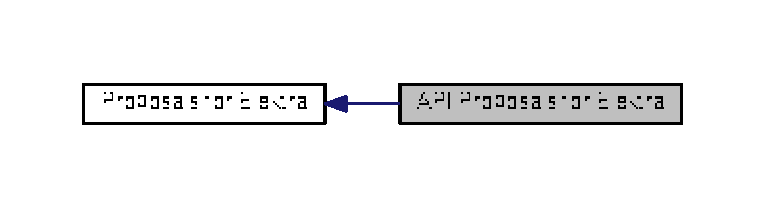
\includegraphics[width=350pt]{group__api}
\end{center}
\end{figure}
\doxysubsection*{Functions}
\begin{DoxyCompactItemize}
\item 
ssize\+\_\+t \mbox{\hyperlink{group__api_ga812eb6c4f506dafa5733bf531c52199c}{key\+Set\+StringF}} (Key $\ast$key, const char $\ast$format,...)
\begin{DoxyCompactList}\small\item\em Set a formatted string. \end{DoxyCompactList}\item 
Key\+Set $\ast$ \mbox{\hyperlink{group__api_ga48120f254e09e0c5cceff4864f110ceb}{elektra\+Key\+Get\+Meta\+Key\+Set}} (const Key $\ast$key)
\begin{DoxyCompactList}\small\item\em Return metadata as keyset. \end{DoxyCompactList}\item 
Key $\ast$ \mbox{\hyperlink{group__api_ga32f8e3258033e970589f23d9d7102bd1}{ks\+Pop\+At\+Cursor}} (Key\+Set $\ast$ks, cursor\+\_\+t pos)
\begin{DoxyCompactList}\small\item\em Pop key at given cursor position. \end{DoxyCompactList}\end{DoxyCompactItemize}


\doxysubsection{Detailed Description}
for kdb.\+h. 

\begin{DoxyWarning}{Warning}
Do not use these methods if you do not want to depend on exactly the Elektra version your binary was built for.
\end{DoxyWarning}
These methods are a technical preview of what might be added in future Elektra releases. It is a requirement that methods are first added here, before they are added to the public A\+PI.

Usually, names in proposal stage should be prefixed with elektra to clearly mark that the signature is likely to be changed and not yet A\+BI compatible. 

\doxysubsection{Function Documentation}
\mbox{\Hypertarget{group__api_ga48120f254e09e0c5cceff4864f110ceb}\label{group__api_ga48120f254e09e0c5cceff4864f110ceb}} 
\index{API Proposals for Elektra@{API Proposals for Elektra}!elektraKeyGetMetaKeySet@{elektraKeyGetMetaKeySet}}
\index{elektraKeyGetMetaKeySet@{elektraKeyGetMetaKeySet}!API Proposals for Elektra@{API Proposals for Elektra}}
\doxysubsubsection{\texorpdfstring{elektraKeyGetMetaKeySet()}{elektraKeyGetMetaKeySet()}}
{\footnotesize\ttfamily Key\+Set$\ast$ elektra\+Key\+Get\+Meta\+Key\+Set (\begin{DoxyParamCaption}\item[{const Key $\ast$}]{key }\end{DoxyParamCaption})}



Return metadata as keyset. 


\begin{DoxyParams}{Parameters}
{\em key} & the key object to work with\\
\hline
\end{DoxyParams}
\begin{DoxyReturn}{Returns}
a duplication of the keyset representing the metadata 
\end{DoxyReturn}
\mbox{\Hypertarget{group__api_ga812eb6c4f506dafa5733bf531c52199c}\label{group__api_ga812eb6c4f506dafa5733bf531c52199c}} 
\index{API Proposals for Elektra@{API Proposals for Elektra}!keySetStringF@{keySetStringF}}
\index{keySetStringF@{keySetStringF}!API Proposals for Elektra@{API Proposals for Elektra}}
\doxysubsubsection{\texorpdfstring{keySetStringF()}{keySetStringF()}}
{\footnotesize\ttfamily ssize\+\_\+t key\+Set\+StringF (\begin{DoxyParamCaption}\item[{Key $\ast$}]{key,  }\item[{const char $\ast$}]{format,  }\item[{}]{... }\end{DoxyParamCaption})}



Set a formatted string. 


\begin{DoxyParams}{Parameters}
{\em key} & the key to set the string value \\
\hline
{\em format} & N\+U\+L\+L-\/terminated text format string \\
\hline
{\em ...} & more arguments\\
\hline
\end{DoxyParams}
\begin{DoxyReturn}{Returns}
the size of the string as set (with including 0) 
\end{DoxyReturn}
\mbox{\Hypertarget{group__api_ga32f8e3258033e970589f23d9d7102bd1}\label{group__api_ga32f8e3258033e970589f23d9d7102bd1}} 
\index{API Proposals for Elektra@{API Proposals for Elektra}!ksPopAtCursor@{ksPopAtCursor}}
\index{ksPopAtCursor@{ksPopAtCursor}!API Proposals for Elektra@{API Proposals for Elektra}}
\doxysubsubsection{\texorpdfstring{ksPopAtCursor()}{ksPopAtCursor()}}
{\footnotesize\ttfamily Key$\ast$ ks\+Pop\+At\+Cursor (\begin{DoxyParamCaption}\item[{Key\+Set $\ast$}]{ks,  }\item[{cursor\+\_\+t}]{pos }\end{DoxyParamCaption})}



Pop key at given cursor position. 


\begin{DoxyParams}{Parameters}
{\em ks} & the keyset to pop key from \\
\hline
{\em c} & where to pop\\
\hline
\end{DoxyParams}
The internal cursor will be rewinded using \mbox{\hyperlink{group__keyset_gabe793ff51f1728e3429c84a8a9086b70}{ks\+Rewind()}}. You can use \mbox{\hyperlink{group__keyset_gaffe507ab9281c322eb16c3e992075d29}{ks\+Get\+Cursor()}} and \mbox{\hyperlink{group__keyset_gad94c9ffaa3e8034564c0712fd407c345}{ks\+Set\+Cursor()}} jump back to the previous position. e.\+g. to pop at current position within \mbox{\hyperlink{group__keyset_ga317321c9065b5a4b3e33fe1c399bcec9}{ks\+Next()}} loop\+: 
\begin{DoxyCode}{0}
\DoxyCodeLine{cursor\_t c = \mbox{\hyperlink{group__keyset_gaffe507ab9281c322eb16c3e992075d29}{ksGetCursor}}(ks);}
\DoxyCodeLine{\mbox{\hyperlink{group__key_ga3df95bbc2494e3e6703ece5639be5bb1}{keyDel}} (\mbox{\hyperlink{group__api_ga32f8e3258033e970589f23d9d7102bd1}{ksPopAtCursor}}(ks, c));}
\DoxyCodeLine{\mbox{\hyperlink{group__keyset_gad94c9ffaa3e8034564c0712fd407c345}{ksSetCursor}}(ks, c);}
\DoxyCodeLine{ksPrev(ks); \textcolor{comment}{// to have correct key after next ksNext()}}
\end{DoxyCode}


\begin{DoxyWarning}{Warning}
do not use, will be superseded by external iterator A\+PI
\end{DoxyWarning}
\begin{DoxyReturn}{Returns}
the popped key 
\end{DoxyReturn}

\begin{DoxyRetVals}{Return values}
{\em 0} & if ks is 0 \\
\hline
\end{DoxyRetVals}

\hypertarget{group__kdb}{}\section{K\+DB}
\label{group__kdb}\index{K\+DB@{K\+DB}}


General methods to access the Key database.  


\subsection*{Functions}
\begin{DoxyCompactItemize}
\item 
\mbox{\Hypertarget{group__kdb_ga5bfaad0230457cd6386032fe65c41576}\label{group__kdb_ga5bfaad0230457cd6386032fe65c41576}} 
int \hyperlink{group__kdb_ga5bfaad0230457cd6386032fe65c41576}{elektra\+Open\+Bootstrap} (K\+DB $\ast$handle, Key\+Set $\ast$keys, Key $\ast$error\+Key)
\begin{DoxyCompactList}\small\item\em Bootstrap, first phase with fallback. \end{DoxyCompactList}\item 
K\+DB $\ast$ \hyperlink{group__kdb_ga6808defe5870f328dd17910aacbdc6ca}{kdb\+Open} (Key $\ast$error\+Key)
\begin{DoxyCompactList}\small\item\em Opens the session with the Key database. \end{DoxyCompactList}\item 
int \hyperlink{group__kdb_gadb54dc9fda17ee07deb9444df745c96f}{kdb\+Close} (K\+DB $\ast$handle, Key $\ast$error\+Key)
\begin{DoxyCompactList}\small\item\em Closes the session with the Key database. \end{DoxyCompactList}\item 
int \hyperlink{group__kdb_ga28e385fd9cb7ccfe0b2f1ed2f62453a1}{kdb\+Get} (K\+DB $\ast$handle, Key\+Set $\ast$ks, Key $\ast$parent\+Key)
\begin{DoxyCompactList}\small\item\em Retrieve keys in an atomic and universal way. \end{DoxyCompactList}\item 
int \hyperlink{group__kdb_ga11436b058408f83d303ca5e996832bcf}{kdb\+Set} (K\+DB $\ast$handle, Key\+Set $\ast$ks, Key $\ast$parent\+Key)
\begin{DoxyCompactList}\small\item\em Set keys in an atomic and universal way. \end{DoxyCompactList}\item 
int \hyperlink{group__kdb_ga0955373877575fa21275891518f8ab31}{kdb\+Ensure} (K\+DB $\ast$handle, Key\+Set $\ast$contract, Key $\ast$parent\+Key)
\begin{DoxyCompactList}\small\item\em This function can be used the given K\+DB {\ttfamily handle} meets certain clauses, specified in {\ttfamily contract}. \end{DoxyCompactList}\end{DoxyCompactItemize}


\subsection{Detailed Description}
General methods to access the Key database. 

To use them\+: 
\begin{DoxyCode}
\textcolor{preprocessor}{#include <kdb.h>}
\end{DoxyCode}


The kdb$\ast$() methods are used to access the storage, to get and set \hyperlink{group__keyset}{Key\+Sets}.

Parameters common for all these functions are\+:


\begin{DoxyItemize}
\item {\itshape handle}, as returned by \hyperlink{group__kdb_ga6808defe5870f328dd17910aacbdc6ca}{kdb\+Open()}, need to be passed to every call
\item {\itshape parent\+Key} is used for every call to add warnings and set an error. For \hyperlink{group__kdb_ga28e385fd9cb7ccfe0b2f1ed2f62453a1}{kdb\+Get()} / \hyperlink{group__kdb_ga11436b058408f83d303ca5e996832bcf}{kdb\+Set()} it is used to give an hint which keys should be retrieved/stored.
\end{DoxyItemize}

\begin{DoxyNote}{Note}
The parent\+Key is an obligation for you, but only an hint for K\+DB. K\+DB does not remember anything about the configuration. You need to pass the same configuration back to \hyperlink{group__kdb_ga11436b058408f83d303ca5e996832bcf}{kdb\+Set()}, otherwise parts of the configuration get lost. Only keys below the parent\+Key are subject for change, the rest must be left untouched.
\end{DoxyNote}
K\+DB uses different backend implementations that know the details about how to access the storage. One backend consists of multiple plugins. See \hyperlink{group__plugin}{writing a new plugin } for information about how to write a plugin. Backends are state-\/less regarding the configuration (because of that you must pass back the whole configuration for every backend), but have a state for\+:


\begin{DoxyItemize}
\item a two phase-\/commit
\item a conflict detection (error 30) and
\item optimizations that avoid redoing already done operations.
\end{DoxyItemize}


\begin{DoxyImage}
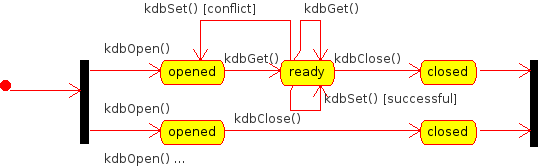
\includegraphics[width=\textwidth,height=\textheight/2,keepaspectratio=true]{state.png}
\doxyfigcaption{State}
\end{DoxyImage}
 As we see in the figure, \hyperlink{group__kdb_ga6808defe5870f328dd17910aacbdc6ca}{kdb\+Open()} can be called arbitrarily often in any number of threads.

For every handle you got from \hyperlink{group__kdb_ga6808defe5870f328dd17910aacbdc6ca}{kdb\+Open()}, for every parent\+Key with a different name, {\itshape only} the shown state transitions are valid. From a freshly opened K\+DB, only \hyperlink{group__kdb_ga28e385fd9cb7ccfe0b2f1ed2f62453a1}{kdb\+Get()} and \hyperlink{group__kdb_gadb54dc9fda17ee07deb9444df745c96f}{kdb\+Close()} are allowed, because otherwise conflicts (error 30) would not be detected.

Once \hyperlink{group__kdb_ga28e385fd9cb7ccfe0b2f1ed2f62453a1}{kdb\+Get()} was called (for a specific handle+parent\+Key), any number of \hyperlink{group__kdb_ga28e385fd9cb7ccfe0b2f1ed2f62453a1}{kdb\+Get()} and \hyperlink{group__kdb_ga11436b058408f83d303ca5e996832bcf}{kdb\+Set()} can be used with this handle respective parent\+Key, unless \hyperlink{group__kdb_ga11436b058408f83d303ca5e996832bcf}{kdb\+Set()} had a conflict (error 30) with another application. Every affair with K\+DB needs to be finished with \hyperlink{group__kdb_gadb54dc9fda17ee07deb9444df745c96f}{kdb\+Close()}.

The name of the parent\+Key in \hyperlink{group__kdb_ga6808defe5870f328dd17910aacbdc6ca}{kdb\+Open()} and \hyperlink{group__kdb_gadb54dc9fda17ee07deb9444df745c96f}{kdb\+Close()} does not matter.

In the usual case we just have one parent\+Key and one handle. In these cases we just have to remember to use \hyperlink{group__kdb_ga28e385fd9cb7ccfe0b2f1ed2f62453a1}{kdb\+Get()} before \hyperlink{group__kdb_ga11436b058408f83d303ca5e996832bcf}{kdb\+Set()}\+:


\begin{DoxyCodeInclude}

\textcolor{preprocessor}{#include <kdb.h>}

\textcolor{keywordtype}{int} \hyperlink{testio__doc_8c_a3c04138a5bfe5d72780bb7e82a18e627}{main} (\textcolor{keywordtype}{void})
\{
        KeySet * myConfig = \hyperlink{group__keyset_ga671e1aaee3ae9dc13b4834a4ddbd2c3c}{ksNew} (0, \hyperlink{kdbenum_8c_a7a28fce3773b2c873c94ac80b8b4cd54}{KS\_END});
        Key * parentKey = \hyperlink{group__key_gad23c65b44bf48d773759e1f9a4d43b89}{keyNew} (\textcolor{stringliteral}{"/sw/MyApp"}, \hyperlink{group__key_gga91fb3178848bd682000958089abbaf40afc1567f74444ff9c219f7456b652b4ec}{KEY\_CASCADING\_NAME}, 
      \hyperlink{group__key_gga91fb3178848bd682000958089abbaf40aa8adb6fcb92dec58fb19410eacfdd403}{KEY\_END});
        KDB * handle = \hyperlink{group__kdb_ga6808defe5870f328dd17910aacbdc6ca}{kdbOpen} (parentKey);

        \hyperlink{group__kdb_ga28e385fd9cb7ccfe0b2f1ed2f62453a1}{kdbGet} (handle, myConfig, parentKey); \textcolor{comment}{// kdbGet() must be first}
        \textcolor{comment}{// now any number of any kdbGet()/kdbSet() calls are allowed, e.g.:}
        \hyperlink{group__kdb_ga11436b058408f83d303ca5e996832bcf}{kdbSet} (handle, myConfig, parentKey);

        \hyperlink{group__keyset_ga27e5c16473b02a422238c8d970db7ac8}{ksDel} (myConfig); \textcolor{comment}{// delete the in-memory configuration}

        \hyperlink{group__kdb_gadb54dc9fda17ee07deb9444df745c96f}{kdbClose} (handle, parentKey); \textcolor{comment}{// no more affairs with the key database.}
        \hyperlink{group__key_ga3df95bbc2494e3e6703ece5639be5bb1}{keyDel} (parentKey);          \textcolor{comment}{// working with key/ks does not need kdb}
\}
\end{DoxyCodeInclude}


To output warnings, you can use following code\+:


\begin{DoxyCodeInclude}
        \textcolor{keyword}{const} Key * metaWarnings = \hyperlink{group__keymeta_ga9ed3875495ddb3d8a8d29158a60a147c}{keyGetMeta} (warningKey, \textcolor{stringliteral}{"warnings"});
        \textcolor{keywordflow}{if} (!metaWarnings) \textcolor{keywordflow}{return} 1; \textcolor{comment}{/* There are no current warnings */}

        \textcolor{keywordtype}{int} nrWarnings = atoi (\hyperlink{group__keyvalue_ga880936f2481d28e6e2acbe7486a21d05}{keyString} (metaWarnings));

        printf (\textcolor{stringliteral}{"There are %d warnings\(\backslash\)n"}, nrWarnings + 1);
        \textcolor{keywordflow}{for} (\textcolor{keywordtype}{int} i = 0; i <= nrWarnings; ++i)
        \{
                \textcolor{keywordtype}{char} buffer[] = \textcolor{stringliteral}{"warnings/#00\(\backslash\)0description"};
                buffer[10] = i / 10 % 10 + \textcolor{charliteral}{'0'};
                buffer[11] = i % 10 + \textcolor{charliteral}{'0'};
                printf (\textcolor{stringliteral}{"buffer is: %s\(\backslash\)n"}, buffer);
                strncat (buffer, \textcolor{stringliteral}{"/number"}, \textcolor{keyword}{sizeof} (buffer) - strlen (buffer) - 1);
                printf (\textcolor{stringliteral}{"number: %s\(\backslash\)n"}, \hyperlink{group__keyvalue_ga880936f2481d28e6e2acbe7486a21d05}{keyString} (\hyperlink{group__keymeta_ga9ed3875495ddb3d8a8d29158a60a147c}{keyGetMeta} (warningKey, buffer)));
                buffer[12] = \textcolor{charliteral}{'\(\backslash\)0'};
                strncat (buffer, \textcolor{stringliteral}{"/description"}, \textcolor{keyword}{sizeof} (buffer) - strlen (buffer) - 1);
                printf (\textcolor{stringliteral}{"description: %s\(\backslash\)n"}, \hyperlink{group__keyvalue_ga880936f2481d28e6e2acbe7486a21d05}{keyString} (\hyperlink{group__keymeta_ga9ed3875495ddb3d8a8d29158a60a147c}{keyGetMeta} (warningKey, buffer))
      );
                buffer[12] = \textcolor{charliteral}{'\(\backslash\)0'};
                strncat (buffer, \textcolor{stringliteral}{"/module"}, \textcolor{keyword}{sizeof} (buffer) - strlen (buffer) - 1);
                \hyperlink{group__keymeta_ga9ed3875495ddb3d8a8d29158a60a147c}{keyGetMeta} (warningKey, buffer);
                printf (\textcolor{stringliteral}{"module: %s\(\backslash\)n"}, \hyperlink{group__keyvalue_ga880936f2481d28e6e2acbe7486a21d05}{keyString} (\hyperlink{group__keymeta_ga9ed3875495ddb3d8a8d29158a60a147c}{keyGetMeta} (warningKey, buffer)));
                buffer[12] = \textcolor{charliteral}{'\(\backslash\)0'};
                strncat (buffer, \textcolor{stringliteral}{"/file"}, \textcolor{keyword}{sizeof} (buffer) - strlen (buffer) - 1);
                \hyperlink{group__keymeta_ga9ed3875495ddb3d8a8d29158a60a147c}{keyGetMeta} (warningKey, buffer);
                printf (\textcolor{stringliteral}{"file: %s\(\backslash\)n"}, \hyperlink{group__keyvalue_ga880936f2481d28e6e2acbe7486a21d05}{keyString} (\hyperlink{group__keymeta_ga9ed3875495ddb3d8a8d29158a60a147c}{keyGetMeta} (warningKey, buffer)));
                buffer[12] = \textcolor{charliteral}{'\(\backslash\)0'};
                strncat (buffer, \textcolor{stringliteral}{"/line"}, \textcolor{keyword}{sizeof} (buffer) - strlen (buffer) - 1);
                \hyperlink{group__keymeta_ga9ed3875495ddb3d8a8d29158a60a147c}{keyGetMeta} (warningKey, buffer);
                printf (\textcolor{stringliteral}{"line: %s\(\backslash\)n"}, \hyperlink{group__keyvalue_ga880936f2481d28e6e2acbe7486a21d05}{keyString} (\hyperlink{group__keymeta_ga9ed3875495ddb3d8a8d29158a60a147c}{keyGetMeta} (warningKey, buffer)));
                buffer[12] = \textcolor{charliteral}{'\(\backslash\)0'};
                strncat (buffer, \textcolor{stringliteral}{"/reason"}, \textcolor{keyword}{sizeof} (buffer) - strlen (buffer) - 1);
                \hyperlink{group__keymeta_ga9ed3875495ddb3d8a8d29158a60a147c}{keyGetMeta} (warningKey, buffer);
                printf (\textcolor{stringliteral}{"reason: %s\(\backslash\)n"}, \hyperlink{group__keyvalue_ga880936f2481d28e6e2acbe7486a21d05}{keyString} (\hyperlink{group__keymeta_ga9ed3875495ddb3d8a8d29158a60a147c}{keyGetMeta} (warningKey, buffer)));
                buffer[12] = \textcolor{charliteral}{'\(\backslash\)0'};
                strncat (buffer, \textcolor{stringliteral}{"/mountpoint"}, \textcolor{keyword}{sizeof} (buffer) - strlen (buffer) - 1);
                \hyperlink{group__keymeta_ga9ed3875495ddb3d8a8d29158a60a147c}{keyGetMeta} (warningKey, buffer);
                printf (\textcolor{stringliteral}{"reason: %s\(\backslash\)n"}, \hyperlink{group__keyvalue_ga880936f2481d28e6e2acbe7486a21d05}{keyString} (\hyperlink{group__keymeta_ga9ed3875495ddb3d8a8d29158a60a147c}{keyGetMeta} (warningKey, buffer)));
                buffer[12] = \textcolor{charliteral}{'\(\backslash\)0'};
                strncat (buffer, \textcolor{stringliteral}{"/configfile"}, \textcolor{keyword}{sizeof} (buffer) - strlen (buffer) - 1);
                \hyperlink{group__keymeta_ga9ed3875495ddb3d8a8d29158a60a147c}{keyGetMeta} (warningKey, buffer);
                printf (\textcolor{stringliteral}{"reason: %s\(\backslash\)n"}, \hyperlink{group__keyvalue_ga880936f2481d28e6e2acbe7486a21d05}{keyString} (\hyperlink{group__keymeta_ga9ed3875495ddb3d8a8d29158a60a147c}{keyGetMeta} (warningKey, buffer)));
        \}
\end{DoxyCodeInclude}
 To output the error, you can use following code\+:


\begin{DoxyCodeInclude}
        \textcolor{keyword}{const} Key * metaError = \hyperlink{group__keymeta_ga9ed3875495ddb3d8a8d29158a60a147c}{keyGetMeta} (errorKey, \textcolor{stringliteral}{"error"});
        \textcolor{keywordflow}{if} (!metaError) \textcolor{keywordflow}{return} 1; \textcolor{comment}{/* There is no current error */}

        printf (\textcolor{stringliteral}{"number: %s\(\backslash\)n"}, \hyperlink{group__keyvalue_ga880936f2481d28e6e2acbe7486a21d05}{keyString} (\hyperlink{group__keymeta_ga9ed3875495ddb3d8a8d29158a60a147c}{keyGetMeta} (errorKey, \textcolor{stringliteral}{"error/number"})));
        printf (\textcolor{stringliteral}{"description: : %s\(\backslash\)n"}, \hyperlink{group__keyvalue_ga880936f2481d28e6e2acbe7486a21d05}{keyString} (\hyperlink{group__keymeta_ga9ed3875495ddb3d8a8d29158a60a147c}{keyGetMeta} (errorKey, \textcolor{stringliteral}{"
      error/description"})));
        printf (\textcolor{stringliteral}{"module: : %s\(\backslash\)n"}, \hyperlink{group__keyvalue_ga880936f2481d28e6e2acbe7486a21d05}{keyString} (\hyperlink{group__keymeta_ga9ed3875495ddb3d8a8d29158a60a147c}{keyGetMeta} (errorKey, \textcolor{stringliteral}{"error/module"})));
        printf (\textcolor{stringliteral}{"at: %s:%s\(\backslash\)n"}, \hyperlink{group__keyvalue_ga880936f2481d28e6e2acbe7486a21d05}{keyString} (\hyperlink{group__keymeta_ga9ed3875495ddb3d8a8d29158a60a147c}{keyGetMeta} (errorKey, \textcolor{stringliteral}{"error/file"})), 
      \hyperlink{group__keyvalue_ga880936f2481d28e6e2acbe7486a21d05}{keyString} (\hyperlink{group__keymeta_ga9ed3875495ddb3d8a8d29158a60a147c}{keyGetMeta} (errorKey, \textcolor{stringliteral}{"error/line"})));
        printf (\textcolor{stringliteral}{"reason: : %s\(\backslash\)n"}, \hyperlink{group__keyvalue_ga880936f2481d28e6e2acbe7486a21d05}{keyString} (\hyperlink{group__keymeta_ga9ed3875495ddb3d8a8d29158a60a147c}{keyGetMeta} (errorKey, \textcolor{stringliteral}{"error/reason"})));
        printf (\textcolor{stringliteral}{"mountpoint: : %s\(\backslash\)n"}, \hyperlink{group__keyvalue_ga880936f2481d28e6e2acbe7486a21d05}{keyString} (\hyperlink{group__keymeta_ga9ed3875495ddb3d8a8d29158a60a147c}{keyGetMeta} (errorKey, \textcolor{stringliteral}{"error/mountpoint
      "})));
        printf (\textcolor{stringliteral}{"configfile: : %s\(\backslash\)n"}, \hyperlink{group__keyvalue_ga880936f2481d28e6e2acbe7486a21d05}{keyString} (\hyperlink{group__keymeta_ga9ed3875495ddb3d8a8d29158a60a147c}{keyGetMeta} (errorKey, \textcolor{stringliteral}{"error/configfile
      "})));
\end{DoxyCodeInclude}


\subsection{Function Documentation}
\mbox{\Hypertarget{group__kdb_gadb54dc9fda17ee07deb9444df745c96f}\label{group__kdb_gadb54dc9fda17ee07deb9444df745c96f}} 
\index{K\+DB@{K\+DB}!kdb\+Close@{kdb\+Close}}
\index{kdb\+Close@{kdb\+Close}!K\+DB@{K\+DB}}
\subsubsection{\texorpdfstring{kdb\+Close()}{kdbClose()}}
{\footnotesize\ttfamily int kdb\+Close (\begin{DoxyParamCaption}\item[{K\+DB $\ast$}]{handle,  }\item[{Key $\ast$}]{error\+Key }\end{DoxyParamCaption})}



Closes the session with the Key database. 

\begin{DoxyPrecond}{Precondition}
The handle must be a valid handle as returned from \hyperlink{group__kdb_ga6808defe5870f328dd17910aacbdc6ca}{kdb\+Open()}

error\+Key must be a valid key, e.\+g. created with \hyperlink{group__key_gad23c65b44bf48d773759e1f9a4d43b89}{key\+New()}
\end{DoxyPrecond}
This is the counterpart of \hyperlink{group__kdb_ga6808defe5870f328dd17910aacbdc6ca}{kdb\+Open()}.

You must call this method when you finished your affairs with the key database. You can manipulate Key and Key\+Set objects also after \hyperlink{group__kdb_gadb54dc9fda17ee07deb9444df745c96f}{kdb\+Close()}, but you must not use any kdb$\ast$() call afterwards.

The {\ttfamily handle} parameter will be finalized and all resources associated to it will be freed. After a \hyperlink{group__kdb_gadb54dc9fda17ee07deb9444df745c96f}{kdb\+Close()}, the {\ttfamily handle} cannot be used anymore.


\begin{DoxyParams}{Parameters}
{\em handle} & contains internal information of \hyperlink{group__kdb_ga6808defe5870f328dd17910aacbdc6ca}{opened } key database \\
\hline
{\em error\+Key} & the key which holds error/warning information \\
\hline
\end{DoxyParams}

\begin{DoxyRetVals}{Return values}
{\em 0} & on success \\
\hline
{\em -\/1} & on N\+U\+LL pointer \\
\hline
\end{DoxyRetVals}
\mbox{\Hypertarget{group__kdb_ga0955373877575fa21275891518f8ab31}\label{group__kdb_ga0955373877575fa21275891518f8ab31}} 
\index{K\+DB@{K\+DB}!kdb\+Ensure@{kdb\+Ensure}}
\index{kdb\+Ensure@{kdb\+Ensure}!K\+DB@{K\+DB}}
\subsubsection{\texorpdfstring{kdb\+Ensure()}{kdbEnsure()}}
{\footnotesize\ttfamily int kdb\+Ensure (\begin{DoxyParamCaption}\item[{K\+DB $\ast$}]{handle,  }\item[{Key\+Set $\ast$}]{contract,  }\item[{Key $\ast$}]{parent\+Key }\end{DoxyParamCaption})}



This function can be used the given K\+DB {\ttfamily handle} meets certain clauses, specified in {\ttfamily contract}. 

Currently the following clauses are supported\+:


\begin{DoxyItemize}
\item {\ttfamily system/elektra/ensure/plugins/$<$mountpoint$>$/$<$pluginname$>$} defines the state of the plugin {\ttfamily $<$pluginname$>$} for the mountpoint {\ttfamily $<$mountpoint$>$}\+:
\begin{DoxyItemize}
\item The value {\ttfamily unmounted} ensures the plugin is not mounted, at this mountpoint.
\item The value {\ttfamily mounted} ensures the plugin is mounted, at this mountpoint. If the plugin is not mounted, we will try to mount it.
\item The value {\ttfamily remount} always mounts the plugin, at this mountpoint. If it was already mounted, it will me unmounted and mounted again. This can be used to ensure the plugin is mounted with a certain configuration.
\end{DoxyItemize}
\item Keys below {\ttfamily system/elektra/ensure/plugins/$<$mountpoint$>$/$<$pluginname$>$/config} are extracted and used as the plugins config Key\+Set during mounting. {\ttfamily system/elektra/ensure/plugins/$<$mountpoint$>$/$<$pluginname$>$} will be repleced by {\ttfamily user} in the keynames. If no keys are given, an empty Key\+Set is used.
\end{DoxyItemize}

There are a few special values for {\ttfamily $<$mountpoint$>$}\+:
\begin{DoxyItemize}
\item {\ttfamily global} is used to indicate the plugin should (un)mounted as a global plugin. Currently this only supports (un)mounting plugins from/to the subposition {\ttfamily maxonce}.
\item {\ttfamily parent} is used to indicate the keyname of {\ttfamily parent\+Key} shall be used as the mountpoint.
\end{DoxyItemize}

If {\ttfamily $<$mountpoint$>$} is none of those values, it has to be valid keyname with the slashes escaped. That means it has to start with {\ttfamily /}, {\ttfamily user}, {\ttfamily system}, {\ttfamily dir} or {\ttfamily spec}.

If {\ttfamily $<$mountpoint$>$} is N\+OT {\ttfamily global}, currently only {\ttfamily unmounted} is supported (not {\ttfamily mounted} and {\ttfamily remounted}).

N\+O\+TE\+: This function only works properly, if the list plugin is mounted in all global positions. If this is not the case, 1 will be returned, because this is seen as an implicit clause in the contract. Additionally any contract that specifies clauses for the list plugin is rejected as malformed.


\begin{DoxyParams}{Parameters}
{\em handle} & contains internal information of \hyperlink{group__kdb_ga6808defe5870f328dd17910aacbdc6ca}{opened } key database \\
\hline
{\em contract} & Key\+Set containing the contract described above. This will always be {\ttfamily \hyperlink{group__keyset_ga27e5c16473b02a422238c8d970db7ac8}{ks\+Del()}}ed. {\bfseries Even in error cases.} \\
\hline
{\em parent\+Key} & The parent\+Key used if the {\ttfamily parent} special value is used, otherwise only used for error reporting.\\
\hline
\end{DoxyParams}

\begin{DoxyRetVals}{Return values}
{\em 0} & on success \\
\hline
{\em 1} & if clauses of the contract are unmet \\
\hline
{\em -\/1} & on N\+U\+LL pointers, or malformed contract \\
\hline
\end{DoxyRetVals}
\mbox{\Hypertarget{group__kdb_ga28e385fd9cb7ccfe0b2f1ed2f62453a1}\label{group__kdb_ga28e385fd9cb7ccfe0b2f1ed2f62453a1}} 
\index{K\+DB@{K\+DB}!kdb\+Get@{kdb\+Get}}
\index{kdb\+Get@{kdb\+Get}!K\+DB@{K\+DB}}
\subsubsection{\texorpdfstring{kdb\+Get()}{kdbGet()}}
{\footnotesize\ttfamily int kdb\+Get (\begin{DoxyParamCaption}\item[{K\+DB $\ast$}]{handle,  }\item[{Key\+Set $\ast$}]{ks,  }\item[{Key $\ast$}]{parent\+Key }\end{DoxyParamCaption})}



Retrieve keys in an atomic and universal way. 

\begin{DoxyPrecond}{Precondition}
The {\ttfamily handle} must be passed as returned from \hyperlink{group__kdb_ga6808defe5870f328dd17910aacbdc6ca}{kdb\+Open()}.

The {\ttfamily returned} Key\+Set must be a valid Key\+Set, e.\+g. constructed with \hyperlink{group__keyset_ga671e1aaee3ae9dc13b4834a4ddbd2c3c}{ks\+New()}.

The {\ttfamily parent\+Key} Key must be a valid Key, e.\+g. constructed with \hyperlink{group__key_gad23c65b44bf48d773759e1f9a4d43b89}{key\+New()}.
\end{DoxyPrecond}
If you pass N\+U\+LL on any parameter \hyperlink{group__kdb_ga28e385fd9cb7ccfe0b2f1ed2f62453a1}{kdb\+Get()} will fail immediately without doing anything.

The {\ttfamily returned} Key\+Set may already contain some keys, e.\+g. from previous \hyperlink{group__kdb_ga28e385fd9cb7ccfe0b2f1ed2f62453a1}{kdb\+Get()} calls. The new retrieved keys will be appended using \hyperlink{group__keyset_gaa5a1d467a4d71041edce68ea7748ce45}{ks\+Append\+Key()}.

If not done earlier \hyperlink{group__kdb_ga28e385fd9cb7ccfe0b2f1ed2f62453a1}{kdb\+Get()} will fully retrieve all keys under the {\ttfamily parent\+Key} folder recursively (See Optimization below when it will not be done).

\begin{DoxyNote}{Note}
\hyperlink{group__kdb_ga28e385fd9cb7ccfe0b2f1ed2f62453a1}{kdb\+Get()} might retrieve more keys than requested (that are not below parent\+Key). These keys must be passed to calls of \hyperlink{group__kdb_ga11436b058408f83d303ca5e996832bcf}{kdb\+Set()}, otherwise they will be lost. This stems from the fact that the user has the only copy of the whole configuration and backends only write configuration that was passed to them. For example, if you \hyperlink{group__kdb_ga28e385fd9cb7ccfe0b2f1ed2f62453a1}{kdb\+Get()} \char`\"{}system/mountpoint/interest\char`\"{} you will not only get all keys below system/mountpoint/interest, but also all keys below system/mountpoint (if system/mountpoint is a mountpoint as the name suggests, but system/mountpoint/interest is not a mountpoint). Make sure to not touch or remove keys outside the keys of interest, because others may need them!
\end{DoxyNote}
\begin{DoxyParagraph}{Example\+:}
This example demonstrates the typical usecase within an application (without error handling).
\end{DoxyParagraph}

\begin{DoxyCodeInclude}

\textcolor{preprocessor}{#include <kdb.h>}
\textcolor{preprocessor}{#include <stdio.h>}

\textcolor{keywordtype}{int} \hyperlink{testio__doc_8c_a3c04138a5bfe5d72780bb7e82a18e627}{main} (\textcolor{keywordtype}{void})
\{
        KeySet * myConfig = \hyperlink{group__keyset_ga671e1aaee3ae9dc13b4834a4ddbd2c3c}{ksNew} (0, \hyperlink{kdbenum_8c_a7a28fce3773b2c873c94ac80b8b4cd54}{KS\_END});

        \textcolor{comment}{// for error handling see kdbget\_error.c}

        \textcolor{comment}{// clang-format off}
\textcolor{comment}{}Key * key = \hyperlink{group__key_gad23c65b44bf48d773759e1f9a4d43b89}{keyNew} (\textcolor{stringliteral}{"/sw/tests/myapp/#0/current/"},  \hyperlink{group__key_gga91fb3178848bd682000958089abbaf40aa8adb6fcb92dec58fb19410eacfdd403}{KEY\_END});
KDB * handle = \hyperlink{group__kdb_ga6808defe5870f328dd17910aacbdc6ca}{kdbOpen} (key);
\hyperlink{group__kdb_ga28e385fd9cb7ccfe0b2f1ed2f62453a1}{kdbGet} (handle, myConfig, key);
Key * result = \hyperlink{group__keyset_gad2e30fb6d4739d917c5abb2ac2f9c1a1}{ksLookupByName} (myConfig, \textcolor{stringliteral}{"/sw/tests/myapp/#0/current/testkey1"}, 0);
        \textcolor{comment}{// clang-format on}

        \hyperlink{group__key_ga3df95bbc2494e3e6703ece5639be5bb1}{keyDel} (key);

        \textcolor{keyword}{const} \textcolor{keywordtype}{char} * key\_name = \hyperlink{group__keyname_ga8e805c726a60da921d3736cda7813513}{keyName} (result);
        \textcolor{keyword}{const} \textcolor{keywordtype}{char} * key\_value = \hyperlink{group__keyvalue_ga880936f2481d28e6e2acbe7486a21d05}{keyString} (result);
        \textcolor{keyword}{const} \textcolor{keywordtype}{char} * key\_comment = \hyperlink{group__keyvalue_ga880936f2481d28e6e2acbe7486a21d05}{keyString} (\hyperlink{group__keymeta_ga9ed3875495ddb3d8a8d29158a60a147c}{keyGetMeta} (result, \textcolor{stringliteral}{"comment"}));
        printf (\textcolor{stringliteral}{"key: %s value: %s comment: %s\(\backslash\)n"}, key\_name, key\_value, key\_comment);

        \hyperlink{group__keyset_ga27e5c16473b02a422238c8d970db7ac8}{ksDel} (myConfig); \textcolor{comment}{// delete the in-memory configuration}


        \textcolor{comment}{// maybe you want kdbSet() myConfig here}

        \hyperlink{group__kdb_gadb54dc9fda17ee07deb9444df745c96f}{kdbClose} (handle, 0); \textcolor{comment}{// no more affairs with the key database.}
\}
\end{DoxyCodeInclude}


When a backend fails \hyperlink{group__kdb_ga28e385fd9cb7ccfe0b2f1ed2f62453a1}{kdb\+Get()} will return -\/1 with all error and warning information in the {\ttfamily parent\+Key}. The parameter {\ttfamily returned} will not be changed.

\begin{DoxyParagraph}{Optimization\+:}
In the first run of kdb\+Get all requested (or more) keys are retrieved. On subsequent calls only the keys are retrieved where something was changed inside the key database. The other keys stay in the Key\+Set returned as passed.
\end{DoxyParagraph}
It is your responsibility to save the original keyset if you need it afterwards.

If you want to be sure to get a fresh keyset again, you need to open a second handle to the key database using \hyperlink{group__kdb_ga6808defe5870f328dd17910aacbdc6ca}{kdb\+Open()}.


\begin{DoxyParams}{Parameters}
{\em handle} & contains internal information of \hyperlink{group__kdb_ga6808defe5870f328dd17910aacbdc6ca}{opened } key database \\
\hline
{\em parent\+Key} & is used to add warnings and set an error information. Additionally, its name is a hint which keys should be retrieved (it is possible that more are retrieved, see Note above).
\begin{DoxyItemize}
\item cascading keys (starting with /) will retrieve the same path in all namespaces
\item / will retrieve all keys 
\end{DoxyItemize}\\
\hline
{\em ks} & the (pre-\/initialized) Key\+Set returned with all keys found will not be changed on error or if no update is required \\
\hline
\end{DoxyParams}
\begin{DoxySeeAlso}{See also}
\hyperlink{group__keyset_gaa34fc43a081e6b01e4120daa6c112004}{ks\+Lookup()}, \hyperlink{group__keyset_gad2e30fb6d4739d917c5abb2ac2f9c1a1}{ks\+Lookup\+By\+Name()} for powerful lookups after the Key\+Set was retrieved 

\hyperlink{group__kdb_ga6808defe5870f328dd17910aacbdc6ca}{kdb\+Open()} which needs to be called before 

\hyperlink{group__kdb_ga11436b058408f83d303ca5e996832bcf}{kdb\+Set()} to save the configuration afterwards and \hyperlink{group__kdb_gadb54dc9fda17ee07deb9444df745c96f}{kdb\+Close()} to finish affairs with the \hyperlink{group__key}{Key} database. 
\end{DoxySeeAlso}

\begin{DoxyRetVals}{Return values}
{\em 1} & if the keys were retrieved successfully \\
\hline
{\em 0} & if there was no update -\/ no changes are made to the keyset then \\
\hline
{\em -\/1} & on failure -\/ no changes are made to the keyset then \\
\hline
\end{DoxyRetVals}
\mbox{\Hypertarget{group__kdb_ga6808defe5870f328dd17910aacbdc6ca}\label{group__kdb_ga6808defe5870f328dd17910aacbdc6ca}} 
\index{K\+DB@{K\+DB}!kdb\+Open@{kdb\+Open}}
\index{kdb\+Open@{kdb\+Open}!K\+DB@{K\+DB}}
\subsubsection{\texorpdfstring{kdb\+Open()}{kdbOpen()}}
{\footnotesize\ttfamily K\+DB$\ast$ kdb\+Open (\begin{DoxyParamCaption}\item[{Key $\ast$}]{error\+Key }\end{DoxyParamCaption})}



Opens the session with the Key database. 

\begin{DoxyPrecond}{Precondition}
error\+Key must be a valid key, e.\+g. created with \hyperlink{group__key_gad23c65b44bf48d773759e1f9a4d43b89}{key\+New()}
\end{DoxyPrecond}
The method will bootstrap itself the following way. The first step is to open the default backend. With it system/elektra/mountpoints will be loaded and all needed libraries and mountpoints will be determined. These libraries for backends will be loaded and with it the {\ttfamily K\+DB} data structure will be initialized.

You must always call this method before retrieving or committing any keys to the database. In the end of the program, after using the key database, you must not forget to \hyperlink{group__kdb_gadb54dc9fda17ee07deb9444df745c96f}{kdb\+Close()}.

The pointer to the {\ttfamily K\+DB} structure returned will be initialized like described above, and it must be passed along on any kdb$\ast$() method your application calls.

Get a {\ttfamily K\+DB} handle for every thread using elektra. Don\textquotesingle{}t share the handle across threads, and also not the pointer accessing it\+:


\begin{DoxyCodeInclude}
\textcolor{keywordtype}{void} thread1 (\textcolor{keywordtype}{void})
\{
        Key * parent = \hyperlink{group__key_gad23c65b44bf48d773759e1f9a4d43b89}{keyNew} (\textcolor{stringliteral}{"/app/part1"}, \hyperlink{group__key_gga91fb3178848bd682000958089abbaf40afc1567f74444ff9c219f7456b652b4ec}{KEY\_CASCADING\_NAME}, 
      \hyperlink{group__key_gga91fb3178848bd682000958089abbaf40aa8adb6fcb92dec58fb19410eacfdd403}{KEY\_END});
        KDB * h = \hyperlink{group__kdb_ga6808defe5870f328dd17910aacbdc6ca}{kdbOpen} (parent);
        \textcolor{comment}{// fetch keys and work with them}
        \hyperlink{group__kdb_gadb54dc9fda17ee07deb9444df745c96f}{kdbClose} (h, parent);
\}
\textcolor{keywordtype}{void} thread2 (\textcolor{keywordtype}{void})
\{
        Key * parent = \hyperlink{group__key_gad23c65b44bf48d773759e1f9a4d43b89}{keyNew} (\textcolor{stringliteral}{"/app/part2"}, \hyperlink{group__key_gga91fb3178848bd682000958089abbaf40afc1567f74444ff9c219f7456b652b4ec}{KEY\_CASCADING\_NAME}, 
      \hyperlink{group__key_gga91fb3178848bd682000958089abbaf40aa8adb6fcb92dec58fb19410eacfdd403}{KEY\_END});
        KDB * h = \hyperlink{group__kdb_ga6808defe5870f328dd17910aacbdc6ca}{kdbOpen} (parent);
        \textcolor{comment}{// fetch keys and work with them}
        \hyperlink{group__kdb_gadb54dc9fda17ee07deb9444df745c96f}{kdbClose} (h, parent);
\}
\end{DoxyCodeInclude}
 You don\textquotesingle{}t need \hyperlink{group__kdb_ga6808defe5870f328dd17910aacbdc6ca}{kdb\+Open()} if you only want to manipulate plain in-\/memory Key or Key\+Set objects.

\begin{DoxyPrecond}{Precondition}
error\+Key must be a valid key, e.\+g. created with \hyperlink{group__key_gad23c65b44bf48d773759e1f9a4d43b89}{key\+New()}
\end{DoxyPrecond}

\begin{DoxyParams}{Parameters}
{\em error\+Key} & the key which holds errors and warnings which were issued \\
\hline
\end{DoxyParams}
\begin{DoxySeeAlso}{See also}
\hyperlink{group__kdb_ga28e385fd9cb7ccfe0b2f1ed2f62453a1}{kdb\+Get()}, \hyperlink{group__kdb_gadb54dc9fda17ee07deb9444df745c96f}{kdb\+Close()} to end all affairs to the \hyperlink{group__key}{Key} database. 
\end{DoxySeeAlso}

\begin{DoxyRetVals}{Return values}
{\em handle} & on success \\
\hline
{\em N\+U\+LL} & on failure \\
\hline
\end{DoxyRetVals}
\mbox{\Hypertarget{group__kdb_ga11436b058408f83d303ca5e996832bcf}\label{group__kdb_ga11436b058408f83d303ca5e996832bcf}} 
\index{K\+DB@{K\+DB}!kdb\+Set@{kdb\+Set}}
\index{kdb\+Set@{kdb\+Set}!K\+DB@{K\+DB}}
\subsubsection{\texorpdfstring{kdb\+Set()}{kdbSet()}}
{\footnotesize\ttfamily int kdb\+Set (\begin{DoxyParamCaption}\item[{K\+DB $\ast$}]{handle,  }\item[{Key\+Set $\ast$}]{ks,  }\item[{Key $\ast$}]{parent\+Key }\end{DoxyParamCaption})}



Set keys in an atomic and universal way. 

\begin{DoxyPrecond}{Precondition}
\hyperlink{group__kdb_ga28e385fd9cb7ccfe0b2f1ed2f62453a1}{kdb\+Get()} must be called before \hyperlink{group__kdb_ga11436b058408f83d303ca5e996832bcf}{kdb\+Set()}\+:
\begin{DoxyItemize}
\item initially (after \hyperlink{group__kdb_ga6808defe5870f328dd17910aacbdc6ca}{kdb\+Open()})
\item after conflict errors in \hyperlink{group__kdb_ga11436b058408f83d303ca5e996832bcf}{kdb\+Set()}.
\end{DoxyItemize}

The {\ttfamily returned} Key\+Set must be a valid Key\+Set, e.\+g. constructed with \hyperlink{group__keyset_ga671e1aaee3ae9dc13b4834a4ddbd2c3c}{ks\+New()}.

The {\ttfamily parent\+Key} Key must be a valid Key, e.\+g. constructed with \hyperlink{group__key_gad23c65b44bf48d773759e1f9a4d43b89}{key\+New()}.
\end{DoxyPrecond}
If you pass N\+U\+LL on any parameter \hyperlink{group__kdb_ga11436b058408f83d303ca5e996832bcf}{kdb\+Set()} will fail immediately without doing anything.

With {\ttfamily parent\+Key} you can give an hint which part of the given keyset is of interest for you. Then you promise to only modify or remove keys below this key. All others would be passed back as they were retrieved by \hyperlink{group__kdb_ga28e385fd9cb7ccfe0b2f1ed2f62453a1}{kdb\+Get()}.

\begin{DoxyParagraph}{Errors}
If some error occurs\+:
\begin{DoxyItemize}
\item \hyperlink{group__kdb_ga11436b058408f83d303ca5e996832bcf}{kdb\+Set()} will leave the Key\+Set\textquotesingle{}s $\ast$ internal cursor on the key that generated the error.
\item Error information will be written into the metadata of the parent key.
\item None of the keys are actually committed in this situation, i.\+e. no configuration file will be modified.
\end{DoxyItemize}
\end{DoxyParagraph}
In case of errors you should present the error message to the user and let the user decide what to do. Possible solutions are\+:
\begin{DoxyItemize}
\item remove the problematic key and use \hyperlink{group__kdb_ga11436b058408f83d303ca5e996832bcf}{kdb\+Set()} again (for validation or type errors)
\item change the value of the problematic key and use \hyperlink{group__kdb_ga11436b058408f83d303ca5e996832bcf}{kdb\+Set()} again (for validation errors)
\item do a \hyperlink{group__kdb_ga28e385fd9cb7ccfe0b2f1ed2f62453a1}{kdb\+Get()} (for conflicts, i.\+e. error 30) and then
\begin{DoxyItemize}
\item set the same keyset again (in favour of what was set by this user)
\item drop the old keyset (in favour of what was set from another application)
\item merge the original, your own and the other keyset
\end{DoxyItemize}
\item export the configuration into a file (for unresolvable errors)
\item repeat the same kdb\+Set might be of limited use if the user does not explicitly request it, because temporary errors are rare and its unlikely that they fix themselves (e.\+g. disc full, permission problems)
\end{DoxyItemize}

\begin{DoxyParagraph}{Optimization}
Each key is checked with \hyperlink{group__keytest_gaf247df0de7aca04b32ef80e39ef12950}{key\+Need\+Sync()} before being actually committed. If no key of a backend needs to be synced any affairs to backends are omitted and 0 is returned.
\end{DoxyParagraph}

\begin{DoxyCodeInclude}
KeySet * myConfig = \hyperlink{group__keyset_ga671e1aaee3ae9dc13b4834a4ddbd2c3c}{ksNew} (0, \hyperlink{kdbenum_8c_a7a28fce3773b2c873c94ac80b8b4cd54}{KS\_END});
Key * parentKey = \hyperlink{group__key_gad23c65b44bf48d773759e1f9a4d43b89}{keyNew} (\textcolor{stringliteral}{"system/sw/MyApp"}, \hyperlink{group__key_gga91fb3178848bd682000958089abbaf40aa8adb6fcb92dec58fb19410eacfdd403}{KEY\_END});
KDB * handle = \hyperlink{group__kdb_ga6808defe5870f328dd17910aacbdc6ca}{kdbOpen} (parentKey);

\hyperlink{group__kdb_ga28e385fd9cb7ccfe0b2f1ed2f62453a1}{kdbGet} (handle, myConfig, parentKey); \textcolor{comment}{// kdbGet needs to be called first!}
KeySet * base = \hyperlink{group__keyset_gac59e4b328245463f1451f68d5106151c}{ksDup} (myConfig);     \textcolor{comment}{// save a copy of original keyset}

\textcolor{comment}{// change the keys within myConfig}

KeySet * ours = \hyperlink{group__keyset_gac59e4b328245463f1451f68d5106151c}{ksDup} (myConfig); \textcolor{comment}{// save a copy of our keyset}
KeySet * theirs;                  \textcolor{comment}{// needed for 3-way merging}
\textcolor{keywordtype}{int} ret = \hyperlink{group__kdb_ga11436b058408f83d303ca5e996832bcf}{kdbSet} (handle, myConfig, parentKey);
\textcolor{keywordflow}{while} (ret == -1) \textcolor{comment}{// as long as we have an error}
\{
        \textcolor{comment}{// We got an error. Warn user.}
        Key * problemKey = \hyperlink{group__keyset_ga4287b9416912c5f2ab9c195cb74fb094}{ksCurrent} (myConfig);
        \textcolor{comment}{// parentKey has the errorInformation}
        \textcolor{comment}{// problemKey is the faulty key (may be null)}
        \textcolor{keywordtype}{int} userInput = showElektraErrorDialog (parentKey, problemKey);
        \textcolor{keywordflow}{switch} (userInput)
        \{
        \textcolor{keywordflow}{case} INPUT\_USE\_OURS:
                \hyperlink{group__kdb_ga28e385fd9cb7ccfe0b2f1ed2f62453a1}{kdbGet} (handle, myConfig, parentKey); \textcolor{comment}{// refresh key database}
                \hyperlink{group__keyset_ga27e5c16473b02a422238c8d970db7ac8}{ksDel} (myConfig);
                myConfig = ours;
                \textcolor{keywordflow}{break};
        \textcolor{keywordflow}{case} INPUT\_DO\_MERGE:
                theirs = \hyperlink{group__keyset_gac59e4b328245463f1451f68d5106151c}{ksDup} (ours);
                \hyperlink{group__kdb_ga28e385fd9cb7ccfe0b2f1ed2f62453a1}{kdbGet} (handle, theirs, parentKey); \textcolor{comment}{// refresh key database}
                KeySet * res = doElektraMerge (ours, theirs, base);
                \hyperlink{group__keyset_ga27e5c16473b02a422238c8d970db7ac8}{ksDel} (theirs);
                myConfig = res;
                \textcolor{keywordflow}{break};
        \textcolor{keywordflow}{case} INPUT\_USE\_THEIRS:
                \textcolor{comment}{// should always work, we just write what we got}
                \textcolor{comment}{// but to be sure always give the user another way}
                \textcolor{comment}{// to exit the loop}
                \hyperlink{group__kdb_ga28e385fd9cb7ccfe0b2f1ed2f62453a1}{kdbGet} (handle, myConfig, parentKey); \textcolor{comment}{// refresh key database}
                \textcolor{keywordflow}{break};
                \textcolor{comment}{// other cases ...}
        \}
        ret = \hyperlink{group__kdb_ga11436b058408f83d303ca5e996832bcf}{kdbSet} (handle, myConfig, parentKey);
\}

\hyperlink{group__keyset_ga27e5c16473b02a422238c8d970db7ac8}{ksDel} (ours);
\hyperlink{group__keyset_ga27e5c16473b02a422238c8d970db7ac8}{ksDel} (base);
\hyperlink{group__keyset_ga27e5c16473b02a422238c8d970db7ac8}{ksDel} (myConfig); \textcolor{comment}{// delete the in-memory configuration}

\hyperlink{group__kdb_gadb54dc9fda17ee07deb9444df745c96f}{kdbClose} (handle, parentKey); \textcolor{comment}{// no more affairs with the key database.}
\hyperlink{group__key_ga3df95bbc2494e3e6703ece5639be5bb1}{keyDel} (parentKey);
\end{DoxyCodeInclude}
 show\+Elektra\+Error\+Dialog() and do\+Elektra\+Merge() need to be implemented by the user of Elektra. For do\+Elektra\+Merge a 3-\/way merge algorithm exists in libelektra-\/tools.


\begin{DoxyParams}{Parameters}
{\em handle} & contains internal information of \hyperlink{group__kdb_ga6808defe5870f328dd17910aacbdc6ca}{opened } key database \\
\hline
{\em ks} & a Key\+Set which should contain changed keys, otherwise nothing is done \\
\hline
{\em parent\+Key} & is used to add warnings and set an error information. Additionally, its name is an hint which keys should be committed (it is possible that more are changed).
\begin{DoxyItemize}
\item cascading keys (starting with /) will set the path in all namespaces
\item / will commit all keys
\item metanames will be rejected (error 104)
\item empty/invalid (error 105) 
\end{DoxyItemize}\\
\hline
\end{DoxyParams}

\begin{DoxyRetVals}{Return values}
{\em 1} & on success \\
\hline
{\em 0} & if nothing had to be done, no changes in K\+DB \\
\hline
{\em -\/1} & on failure, no changes in K\+DB \\
\hline
\end{DoxyRetVals}
\begin{DoxySeeAlso}{See also}
\hyperlink{group__keytest_gaf247df0de7aca04b32ef80e39ef12950}{key\+Need\+Sync()} 

\hyperlink{group__keyset_ga4287b9416912c5f2ab9c195cb74fb094}{ks\+Current()} contains the error \hyperlink{group__key}{Key} 

\hyperlink{group__kdb_ga6808defe5870f328dd17910aacbdc6ca}{kdb\+Open()} and \hyperlink{group__kdb_ga28e385fd9cb7ccfe0b2f1ed2f62453a1}{kdb\+Get()} that must be called first 

\hyperlink{group__kdb_gadb54dc9fda17ee07deb9444df745c96f}{kdb\+Close()} that must be called afterwards 
\end{DoxySeeAlso}

\hypertarget{group__key}{}\doxysection{Key}
\label{group__key}\index{Key@{Key}}


Key is an essential class that encapsulates key \mbox{\hyperlink{group__keyname}{name }}, \mbox{\hyperlink{group__keyvalue}{value }} and \mbox{\hyperlink{group__keymeta}{metainfo }}.  


Collaboration diagram for Key\+:
\nopagebreak
\begin{figure}[H]
\begin{center}
\leavevmode
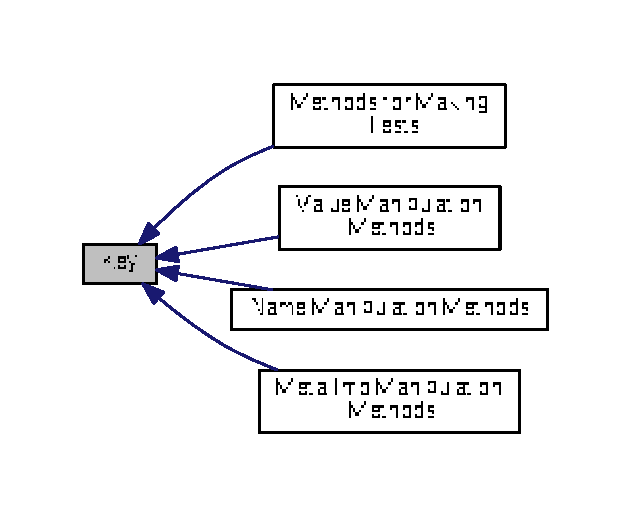
\includegraphics[width=309pt]{group__key}
\end{center}
\end{figure}
\doxysubsection*{Modules}
\begin{DoxyCompactItemize}
\item 
\mbox{\hyperlink{group__keymeta}{Meta Info Manipulation Methods}}
\begin{DoxyCompactList}\small\item\em Methods to do various operations on Key metadata. \end{DoxyCompactList}\item 
\mbox{\hyperlink{group__keytest}{Methods for Making Tests}}
\begin{DoxyCompactList}\small\item\em Methods to do various tests on Keys. \end{DoxyCompactList}\item 
\mbox{\hyperlink{group__keyname}{Name Manipulation Methods}}
\begin{DoxyCompactList}\small\item\em Methods to do various operations on Key names. \end{DoxyCompactList}\item 
\mbox{\hyperlink{group__keyvalue}{Value Manipulation Methods}}
\begin{DoxyCompactList}\small\item\em Methods to do various operations on Key values. \end{DoxyCompactList}\end{DoxyCompactItemize}
\doxysubsection*{Macros}
\begin{DoxyCompactItemize}
\item 
\#define \mbox{\hyperlink{group__key_gad19f92d6d37dc439d1727ca10263c9cc}{KDB\+\_\+\+PATH\+\_\+\+SEPARATOR}}~\textquotesingle{}/\textquotesingle{}
\begin{DoxyCompactList}\small\item\em {\ttfamily /} is used to separate key names. \end{DoxyCompactList}\item 
\#define \mbox{\hyperlink{group__key_ga6d24980bc81c4276367f4e80725a8b61}{KDB\+\_\+\+PATH\+\_\+\+ESCAPE}}~\textquotesingle{}\textbackslash{}\textbackslash{}\textquotesingle{}
\begin{DoxyCompactList}\small\item\em {\ttfamily \textbackslash{}} is used as escape character in the key name. \end{DoxyCompactList}\end{DoxyCompactItemize}
\doxysubsection*{Enumerations}
\begin{DoxyCompactItemize}
\item 
enum \mbox{\hyperlink{group__key_ga9b703ca49f48b482def322b77d3e6bc8}{elektra\+Key\+Flags}} \{ \newline
\mbox{\hyperlink{group__key_gga9b703ca49f48b482def322b77d3e6bc8ad6127fc38f96410bf7c8f6e93b0397da}{KEY\+\_\+\+NAME}} = 1
, \mbox{\hyperlink{group__key_gga9b703ca49f48b482def322b77d3e6bc8ac66e4a49d09212b79f5754ca6db5bd2e}{KEY\+\_\+\+VALUE}} = 1 $<$$<$ 1
, \mbox{\hyperlink{group__key_gga9b703ca49f48b482def322b77d3e6bc8a4b83f86a07a7a0d6e24ecafe43cfea1b}{KEY\+\_\+\+FLAGS}} = 3
, \mbox{\hyperlink{group__key_gga9b703ca49f48b482def322b77d3e6bc8ac29427bb47cc31689d02912e36161ee3}{KEY\+\_\+\+COMMENT}} = 1 $<$$<$ 3
, \newline
\mbox{\hyperlink{group__key_gga9b703ca49f48b482def322b77d3e6bc8a1ca18d4e094ae7487d35ecedda2235ff}{KEY\+\_\+\+BINARY}} = 1 $<$$<$ 4
, \mbox{\hyperlink{group__key_gga9b703ca49f48b482def322b77d3e6bc8a6d531b5c41445d19d0452eebdccbfa01}{KEY\+\_\+\+SIZE}} = 1 $<$$<$ 11
, \mbox{\hyperlink{group__key_gga9b703ca49f48b482def322b77d3e6bc8a040582834bb2d90049947d7ef74e87e2}{KEY\+\_\+\+META}} = 1 $<$$<$ 15
, \mbox{\hyperlink{group__key_gga9b703ca49f48b482def322b77d3e6bc8ab089c5e7977d6e58737eb586ee153b7f}{KEY\+\_\+\+NULL}} = 1 $<$$<$ 16
, \newline
\mbox{\hyperlink{group__key_gga9b703ca49f48b482def322b77d3e6bc8aa8adb6fcb92dec58fb19410eacfdd403}{KEY\+\_\+\+END}} = 0
 \}
\begin{DoxyCompactList}\small\item\em Allows \mbox{\hyperlink{group__key_gad23c65b44bf48d773759e1f9a4d43b89}{key\+New()}} to determine which information comes next. \end{DoxyCompactList}\item 
enum \mbox{\hyperlink{group__key_ga9ff42b1e9a97222562bfda3dd1f8c735}{elektra\+Copy\+Flags}} \{ \newline
\mbox{\hyperlink{group__key_gga9ff42b1e9a97222562bfda3dd1f8c735ab41d70eb97ae5480333e85759318b5a9}{KEY\+\_\+\+CP\+\_\+\+NAME}} = 1 $<$$<$ 0
, \mbox{\hyperlink{group__key_gga9ff42b1e9a97222562bfda3dd1f8c735a57996652569a901d4e7e58c33f7b3631}{KEY\+\_\+\+CP\+\_\+\+STRING}} = 1 $<$$<$ 1
, \mbox{\hyperlink{group__key_gga9ff42b1e9a97222562bfda3dd1f8c735a3043a92bfbe465ccff7624e54d89bcf8}{KEY\+\_\+\+CP\+\_\+\+VALUE}} = 1 $<$$<$ 2
, \mbox{\hyperlink{group__key_gga9ff42b1e9a97222562bfda3dd1f8c735a6b8bdcae98a0f29d66a6b3d1651cbac6}{KEY\+\_\+\+CP\+\_\+\+META}} = 1 $<$$<$ 3
, \newline
\mbox{\hyperlink{group__key_gga9ff42b1e9a97222562bfda3dd1f8c735a3e04e17514f102f1e9217308d44e7612}{KEY\+\_\+\+CP\+\_\+\+ALL}} = KEY\+\_\+\+CP\+\_\+\+NAME $\vert$ KEY\+\_\+\+CP\+\_\+\+VALUE $\vert$ KEY\+\_\+\+CP\+\_\+\+META
 \}
\begin{DoxyCompactList}\small\item\em Copy options. \end{DoxyCompactList}\item 
enum \mbox{\hyperlink{group__key_gafa3306030b1d06b06c3cba24c516f5ec}{elektra\+Lock\+Flags}} \{ \mbox{\hyperlink{group__key_ggafa3306030b1d06b06c3cba24c516f5eca4813b0cfdefeb676e35f599ef763c265}{KEY\+\_\+\+LOCK\+\_\+\+NAME}} = 1 $<$$<$ 17
, \mbox{\hyperlink{group__key_ggafa3306030b1d06b06c3cba24c516f5eca4ed4895f3f243287f7adef621815d7e6}{KEY\+\_\+\+LOCK\+\_\+\+VALUE}} = 1 $<$$<$ 18
, \mbox{\hyperlink{group__key_ggafa3306030b1d06b06c3cba24c516f5eca4f1b7ee5af7539286d8989a9a5658958}{KEY\+\_\+\+LOCK\+\_\+\+META}} = 1 $<$$<$ 19
 \}
\begin{DoxyCompactList}\small\item\em Lock options. \end{DoxyCompactList}\item 
enum \mbox{\hyperlink{group__key_gaec3b8d6f430ae49b91bafe8a86310a68}{elektra\+Namespace}} \{ \newline
\mbox{\hyperlink{group__key_ggaec3b8d6f430ae49b91bafe8a86310a68a3659698b0a07454ca8055ab693e8efd1}{KEY\+\_\+\+NS\+\_\+\+NONE}} = 0
, \mbox{\hyperlink{group__key_ggaec3b8d6f430ae49b91bafe8a86310a68a2c9133e3095dccbcde5ca3bb13987b5d}{KEY\+\_\+\+NS\+\_\+\+CASCADING}} = 1
, \mbox{\hyperlink{group__key_ggaec3b8d6f430ae49b91bafe8a86310a68ac5fbf2c3a7ae79fa2d60c48ae3e72688}{KEY\+\_\+\+NS\+\_\+\+META}} = 2
, \mbox{\hyperlink{group__key_ggaec3b8d6f430ae49b91bafe8a86310a68a2be047b124b1ca0e92b5ef124169f0d2}{KEY\+\_\+\+NS\+\_\+\+SPEC}} = 3
, \newline
\mbox{\hyperlink{group__key_ggaec3b8d6f430ae49b91bafe8a86310a68a470ecc9254fcdfccf9923a3e526c9c11}{KEY\+\_\+\+NS\+\_\+\+PROC}} = 4
, \mbox{\hyperlink{group__key_ggaec3b8d6f430ae49b91bafe8a86310a68aa0006cf27dbb2586bafba6ff1ae4f4ec}{KEY\+\_\+\+NS\+\_\+\+DIR}} = 5
, \mbox{\hyperlink{group__key_ggaec3b8d6f430ae49b91bafe8a86310a68a8ce23c70010e8ac8bb540b0947e03a4e}{KEY\+\_\+\+NS\+\_\+\+USER}} = 6
, \mbox{\hyperlink{group__key_ggaec3b8d6f430ae49b91bafe8a86310a68a61adca2f9dff47e65dfcdb492ffa7a20}{KEY\+\_\+\+NS\+\_\+\+SYSTEM}} = 7
, \newline
\mbox{\hyperlink{group__key_ggaec3b8d6f430ae49b91bafe8a86310a68ad6792ab14711ed6d6e507ca3d10b05e7}{KEY\+\_\+\+NS\+\_\+\+DEFAULT}} = 8
 \}
\begin{DoxyCompactList}\small\item\em Elektra currently supported Key namespaces. \end{DoxyCompactList}\end{DoxyCompactItemize}
\doxysubsection*{Functions}
\begin{DoxyCompactItemize}
\item 
Key $\ast$ \mbox{\hyperlink{group__key_gad23c65b44bf48d773759e1f9a4d43b89}{key\+New}} (const char $\ast$name,...)
\begin{DoxyCompactList}\small\item\em A practical way to fully create a Key object in one step. \end{DoxyCompactList}\item 
Key $\ast$ \mbox{\hyperlink{group__key_ga505575ebef060066984fe0f590081e37}{key\+Copy}} (Key $\ast$dest, const Key $\ast$source, \mbox{\hyperlink{group__key_ga9ff42b1e9a97222562bfda3dd1f8c735}{elektra\+Copy\+Flags}} flags)
\begin{DoxyCompactList}\small\item\em Copy or clear a key. \end{DoxyCompactList}\item 
int \mbox{\hyperlink{group__key_ga3df95bbc2494e3e6703ece5639be5bb1}{key\+Del}} (Key $\ast$key)
\begin{DoxyCompactList}\small\item\em A destructor for Key objects. \end{DoxyCompactList}\item 
int \mbox{\hyperlink{group__key_gab2242311a36bbc0520e0d36895107ec1}{key\+Clear}} (Key $\ast$key)
\begin{DoxyCompactList}\small\item\em Will clear all internal data of a Key. \end{DoxyCompactList}\item 
ssize\+\_\+t \mbox{\hyperlink{group__key_ga6970a6f254d67af7e39f8e469bb162f1}{key\+Inc\+Ref}} (Key $\ast$key)
\begin{DoxyCompactList}\small\item\em Increment the reference counter of a Key object. \end{DoxyCompactList}\item 
ssize\+\_\+t \mbox{\hyperlink{group__key_ga2c6433ca22109e4e141946057eccb283}{key\+Dec\+Ref}} (Key $\ast$key)
\begin{DoxyCompactList}\small\item\em Decrement the reference counter of a Key object. \end{DoxyCompactList}\item 
ssize\+\_\+t \mbox{\hyperlink{group__key_ga4aabc4272506dd63161db2bbb42de8ae}{key\+Get\+Ref}} (const Key $\ast$key)
\begin{DoxyCompactList}\small\item\em Return how many references the Key has. \end{DoxyCompactList}\item 
int \mbox{\hyperlink{group__key_ga5e42b653a0f117be7f1f6eb06c569bb8}{key\+Lock}} (Key $\ast$key, \mbox{\hyperlink{group__key_gafa3306030b1d06b06c3cba24c516f5ec}{elektra\+Lock\+Flags}} what)
\begin{DoxyCompactList}\small\item\em Permanently lock parts of a Key. \end{DoxyCompactList}\item 
int \mbox{\hyperlink{group__key_ga769882e86e34a95cefcf8f260ef97e06}{key\+Is\+Locked}} (const Key $\ast$key, \mbox{\hyperlink{group__key_gafa3306030b1d06b06c3cba24c516f5ec}{elektra\+Lock\+Flags}} what)
\begin{DoxyCompactList}\small\item\em Checks which parts of a Key are locked. \end{DoxyCompactList}\end{DoxyCompactItemize}


\doxysubsection{Detailed Description}
Key is an essential class that encapsulates key \mbox{\hyperlink{group__keyname}{name }}, \mbox{\hyperlink{group__keyvalue}{value }} and \mbox{\hyperlink{group__keymeta}{metainfo }}. 

To use it include\+: 
\begin{DoxyCode}{0}
\DoxyCodeLine{\textcolor{preprocessor}{\#include <kdb.h>}}

\end{DoxyCode}


Key properties are\+:
\begin{DoxyItemize}
\item \mbox{\hyperlink{group__keyname}{Key name }}
\item \mbox{\hyperlink{group__keyvalue}{Key value }}
\item \mbox{\hyperlink{group__keymeta}{Key metadata }}, including but not limited to\+:
\begin{DoxyItemize}
\item \mbox{\hyperlink{group__meta_gafb89735689929ff717cc9f2d0d0b46a2}{Key comment }}
\item \mbox{\hyperlink{}{Key owner }}
\item \mbox{\hyperlink{group__keymeta}{UID, GID and filesystem-\/like mode permissions }}
\item \mbox{\hyperlink{group__keymeta}{Mode, change and modification times }}
\end{DoxyItemize}
\end{DoxyItemize}

\begin{DoxyParagraph}{ABI}
Due to ABI compatibility, the {\ttfamily Key} structure is not defined in kdb.\+h, only declared. So you can only declare {\ttfamily pointers} to {\ttfamily Keys} in your program, and allocate and free memory for them with \mbox{\hyperlink{group__key_gad23c65b44bf48d773759e1f9a4d43b89}{key\+New()}} and \mbox{\hyperlink{group__key_ga3df95bbc2494e3e6703ece5639be5bb1}{key\+Del()}} respectively.
\end{DoxyParagraph}
\begin{DoxyParagraph}{Reference Counting}
Every key has its reference counter (see \mbox{\hyperlink{group__key_ga4aabc4272506dd63161db2bbb42de8ae}{key\+Get\+Ref()}} for longer explanation) that will be initialized with 0, that means a subsequent call of \mbox{\hyperlink{group__key_ga3df95bbc2494e3e6703ece5639be5bb1}{key\+Del()}} will delete the key. If you append the key to a keyset the reference counter will be incremented by one (see \mbox{\hyperlink{group__key_ga6970a6f254d67af7e39f8e469bb162f1}{key\+Inc\+Ref()}}) and the key can\textquotesingle{}t be deleted by a \mbox{\hyperlink{group__key_ga3df95bbc2494e3e6703ece5639be5bb1}{key\+Del()}}.
\end{DoxyParagraph}
\begin{DoxyParagraph}{}
As you can imagine this refcounting allows you to put the Key in your own data structures. It can be a very powerful feature, e.\+g. if you need your own-\/defined ordering or different Models of your configuration. 
\end{DoxyParagraph}


\doxysubsection{Macro Definition Documentation}
\mbox{\Hypertarget{group__key_ga6d24980bc81c4276367f4e80725a8b61}\label{group__key_ga6d24980bc81c4276367f4e80725a8b61}} 
\index{Key@{Key}!KDB\_PATH\_ESCAPE@{KDB\_PATH\_ESCAPE}}
\index{KDB\_PATH\_ESCAPE@{KDB\_PATH\_ESCAPE}!Key@{Key}}
\doxysubsubsection{\texorpdfstring{KDB\_PATH\_ESCAPE}{KDB\_PATH\_ESCAPE}}
{\footnotesize\ttfamily \#define KDB\+\_\+\+PATH\+\_\+\+ESCAPE~\textquotesingle{}\textbackslash{}\textbackslash{}\textquotesingle{}}



{\ttfamily \textbackslash{}} is used as escape character in the key name. 

\begin{DoxySeeAlso}{See also}
\mbox{\hyperlink{group__keyname}{description about key names }}. 
\end{DoxySeeAlso}
\mbox{\Hypertarget{group__key_gad19f92d6d37dc439d1727ca10263c9cc}\label{group__key_gad19f92d6d37dc439d1727ca10263c9cc}} 
\index{Key@{Key}!KDB\_PATH\_SEPARATOR@{KDB\_PATH\_SEPARATOR}}
\index{KDB\_PATH\_SEPARATOR@{KDB\_PATH\_SEPARATOR}!Key@{Key}}
\doxysubsubsection{\texorpdfstring{KDB\_PATH\_SEPARATOR}{KDB\_PATH\_SEPARATOR}}
{\footnotesize\ttfamily \#define KDB\+\_\+\+PATH\+\_\+\+SEPARATOR~\textquotesingle{}/\textquotesingle{}}



{\ttfamily /} is used to separate key names. 

\begin{DoxySeeAlso}{See also}
\mbox{\hyperlink{group__keyname}{description about key names }}. 
\end{DoxySeeAlso}


\doxysubsection{Enumeration Type Documentation}
\mbox{\Hypertarget{group__key_ga9ff42b1e9a97222562bfda3dd1f8c735}\label{group__key_ga9ff42b1e9a97222562bfda3dd1f8c735}} 
\index{Key@{Key}!elektraCopyFlags@{elektraCopyFlags}}
\index{elektraCopyFlags@{elektraCopyFlags}!Key@{Key}}
\doxysubsubsection{\texorpdfstring{elektraCopyFlags}{elektraCopyFlags}}
{\footnotesize\ttfamily enum \mbox{\hyperlink{group__key_ga9ff42b1e9a97222562bfda3dd1f8c735}{elektra\+Copy\+Flags}}}



Copy options. 

\begin{DoxySeeAlso}{See also}
\mbox{\hyperlink{group__key_ga505575ebef060066984fe0f590081e37}{key\+Copy()}} 
\end{DoxySeeAlso}
\begin{DoxyEnumFields}{Enumerator}
\raisebox{\heightof{T}}[0pt][0pt]{\index{KEY\_CP\_NAME@{KEY\_CP\_NAME}!Key@{Key}}\index{Key@{Key}!KEY\_CP\_NAME@{KEY\_CP\_NAME}}}\mbox{\Hypertarget{group__key_gga9ff42b1e9a97222562bfda3dd1f8c735ab41d70eb97ae5480333e85759318b5a9}\label{group__key_gga9ff42b1e9a97222562bfda3dd1f8c735ab41d70eb97ae5480333e85759318b5a9}} 
KEY\+\_\+\+CP\+\_\+\+NAME&Flag for copying the key name \\
\hline

\raisebox{\heightof{T}}[0pt][0pt]{\index{KEY\_CP\_STRING@{KEY\_CP\_STRING}!Key@{Key}}\index{Key@{Key}!KEY\_CP\_STRING@{KEY\_CP\_STRING}}}\mbox{\Hypertarget{group__key_gga9ff42b1e9a97222562bfda3dd1f8c735a57996652569a901d4e7e58c33f7b3631}\label{group__key_gga9ff42b1e9a97222562bfda3dd1f8c735a57996652569a901d4e7e58c33f7b3631}} 
KEY\+\_\+\+CP\+\_\+\+STRING&Flag for copying the key value, if it is a string \\
\hline

\raisebox{\heightof{T}}[0pt][0pt]{\index{KEY\_CP\_VALUE@{KEY\_CP\_VALUE}!Key@{Key}}\index{Key@{Key}!KEY\_CP\_VALUE@{KEY\_CP\_VALUE}}}\mbox{\Hypertarget{group__key_gga9ff42b1e9a97222562bfda3dd1f8c735a3043a92bfbe465ccff7624e54d89bcf8}\label{group__key_gga9ff42b1e9a97222562bfda3dd1f8c735a3043a92bfbe465ccff7624e54d89bcf8}} 
KEY\+\_\+\+CP\+\_\+\+VALUE&Flag for copying the key value \\
\hline

\raisebox{\heightof{T}}[0pt][0pt]{\index{KEY\_CP\_META@{KEY\_CP\_META}!Key@{Key}}\index{Key@{Key}!KEY\_CP\_META@{KEY\_CP\_META}}}\mbox{\Hypertarget{group__key_gga9ff42b1e9a97222562bfda3dd1f8c735a6b8bdcae98a0f29d66a6b3d1651cbac6}\label{group__key_gga9ff42b1e9a97222562bfda3dd1f8c735a6b8bdcae98a0f29d66a6b3d1651cbac6}} 
KEY\+\_\+\+CP\+\_\+\+META&Flag for copying the key metadata \\
\hline

\raisebox{\heightof{T}}[0pt][0pt]{\index{KEY\_CP\_ALL@{KEY\_CP\_ALL}!Key@{Key}}\index{Key@{Key}!KEY\_CP\_ALL@{KEY\_CP\_ALL}}}\mbox{\Hypertarget{group__key_gga9ff42b1e9a97222562bfda3dd1f8c735a3e04e17514f102f1e9217308d44e7612}\label{group__key_gga9ff42b1e9a97222562bfda3dd1f8c735a3e04e17514f102f1e9217308d44e7612}} 
KEY\+\_\+\+CP\+\_\+\+ALL&Shorthand for copying name, value and metadata \\
\hline

\end{DoxyEnumFields}
\mbox{\Hypertarget{group__key_ga9b703ca49f48b482def322b77d3e6bc8}\label{group__key_ga9b703ca49f48b482def322b77d3e6bc8}} 
\index{Key@{Key}!elektraKeyFlags@{elektraKeyFlags}}
\index{elektraKeyFlags@{elektraKeyFlags}!Key@{Key}}
\doxysubsubsection{\texorpdfstring{elektraKeyFlags}{elektraKeyFlags}}
{\footnotesize\ttfamily enum \mbox{\hyperlink{group__key_ga9b703ca49f48b482def322b77d3e6bc8}{elektra\+Key\+Flags}}}



Allows \mbox{\hyperlink{group__key_gad23c65b44bf48d773759e1f9a4d43b89}{key\+New()}} to determine which information comes next. 

\begin{DoxySeeAlso}{See also}
\mbox{\hyperlink{group__key_gad23c65b44bf48d773759e1f9a4d43b89}{key\+New()}} 
\end{DoxySeeAlso}
\begin{DoxyEnumFields}{Enumerator}
\raisebox{\heightof{T}}[0pt][0pt]{\index{KEY\_NAME@{KEY\_NAME}!Key@{Key}}\index{Key@{Key}!KEY\_NAME@{KEY\_NAME}}}\mbox{\Hypertarget{group__key_gga9b703ca49f48b482def322b77d3e6bc8ad6127fc38f96410bf7c8f6e93b0397da}\label{group__key_gga9b703ca49f48b482def322b77d3e6bc8ad6127fc38f96410bf7c8f6e93b0397da}} 
KEY\+\_\+\+NAME&Flag for the key name \\
\hline

\raisebox{\heightof{T}}[0pt][0pt]{\index{KEY\_VALUE@{KEY\_VALUE}!Key@{Key}}\index{Key@{Key}!KEY\_VALUE@{KEY\_VALUE}}}\mbox{\Hypertarget{group__key_gga9b703ca49f48b482def322b77d3e6bc8ac66e4a49d09212b79f5754ca6db5bd2e}\label{group__key_gga9b703ca49f48b482def322b77d3e6bc8ac66e4a49d09212b79f5754ca6db5bd2e}} 
KEY\+\_\+\+VALUE&Flag for the key data \\
\hline

\raisebox{\heightof{T}}[0pt][0pt]{\index{KEY\_FLAGS@{KEY\_FLAGS}!Key@{Key}}\index{Key@{Key}!KEY\_FLAGS@{KEY\_FLAGS}}}\mbox{\Hypertarget{group__key_gga9b703ca49f48b482def322b77d3e6bc8a4b83f86a07a7a0d6e24ecafe43cfea1b}\label{group__key_gga9b703ca49f48b482def322b77d3e6bc8a4b83f86a07a7a0d6e24ecafe43cfea1b}} 
KEY\+\_\+\+FLAGS&Allows to define multiple flags at once. \\
\hline

\raisebox{\heightof{T}}[0pt][0pt]{\index{KEY\_COMMENT@{KEY\_COMMENT}!Key@{Key}}\index{Key@{Key}!KEY\_COMMENT@{KEY\_COMMENT}}}\mbox{\Hypertarget{group__key_gga9b703ca49f48b482def322b77d3e6bc8ac29427bb47cc31689d02912e36161ee3}\label{group__key_gga9b703ca49f48b482def322b77d3e6bc8ac29427bb47cc31689d02912e36161ee3}} 
KEY\+\_\+\+COMMENT&Flag for the key comment \\
\hline

\raisebox{\heightof{T}}[0pt][0pt]{\index{KEY\_BINARY@{KEY\_BINARY}!Key@{Key}}\index{Key@{Key}!KEY\_BINARY@{KEY\_BINARY}}}\mbox{\Hypertarget{group__key_gga9b703ca49f48b482def322b77d3e6bc8a1ca18d4e094ae7487d35ecedda2235ff}\label{group__key_gga9b703ca49f48b482def322b77d3e6bc8a1ca18d4e094ae7487d35ecedda2235ff}} 
KEY\+\_\+\+BINARY&Flag if the key is binary \\
\hline

\raisebox{\heightof{T}}[0pt][0pt]{\index{KEY\_SIZE@{KEY\_SIZE}!Key@{Key}}\index{Key@{Key}!KEY\_SIZE@{KEY\_SIZE}}}\mbox{\Hypertarget{group__key_gga9b703ca49f48b482def322b77d3e6bc8a6d531b5c41445d19d0452eebdccbfa01}\label{group__key_gga9b703ca49f48b482def322b77d3e6bc8a6d531b5c41445d19d0452eebdccbfa01}} 
KEY\+\_\+\+SIZE&Flag for maximum size to limit value \\
\hline

\raisebox{\heightof{T}}[0pt][0pt]{\index{KEY\_META@{KEY\_META}!Key@{Key}}\index{Key@{Key}!KEY\_META@{KEY\_META}}}\mbox{\Hypertarget{group__key_gga9b703ca49f48b482def322b77d3e6bc8a040582834bb2d90049947d7ef74e87e2}\label{group__key_gga9b703ca49f48b482def322b77d3e6bc8a040582834bb2d90049947d7ef74e87e2}} 
KEY\+\_\+\+META&Flag for metadata \\
\hline

\raisebox{\heightof{T}}[0pt][0pt]{\index{KEY\_NULL@{KEY\_NULL}!Key@{Key}}\index{Key@{Key}!KEY\_NULL@{KEY\_NULL}}}\mbox{\Hypertarget{group__key_gga9b703ca49f48b482def322b77d3e6bc8ab089c5e7977d6e58737eb586ee153b7f}\label{group__key_gga9b703ca49f48b482def322b77d3e6bc8ab089c5e7977d6e58737eb586ee153b7f}} 
KEY\+\_\+\+NULL&Is {\itshape not} a flag, only as return value \begin{DoxyRefDesc}{Deprecated}
\item[\mbox{\hyperlink{deprecated__deprecated000001}{Deprecated}}]do not use \end{DoxyRefDesc}
\\
\hline

\raisebox{\heightof{T}}[0pt][0pt]{\index{KEY\_END@{KEY\_END}!Key@{Key}}\index{Key@{Key}!KEY\_END@{KEY\_END}}}\mbox{\Hypertarget{group__key_gga9b703ca49f48b482def322b77d3e6bc8aa8adb6fcb92dec58fb19410eacfdd403}\label{group__key_gga9b703ca49f48b482def322b77d3e6bc8aa8adb6fcb92dec58fb19410eacfdd403}} 
KEY\+\_\+\+END&Used as a parameter terminator to \mbox{\hyperlink{group__key_gad23c65b44bf48d773759e1f9a4d43b89}{key\+New()}} \\
\hline

\end{DoxyEnumFields}
\mbox{\Hypertarget{group__key_gafa3306030b1d06b06c3cba24c516f5ec}\label{group__key_gafa3306030b1d06b06c3cba24c516f5ec}} 
\index{Key@{Key}!elektraLockFlags@{elektraLockFlags}}
\index{elektraLockFlags@{elektraLockFlags}!Key@{Key}}
\doxysubsubsection{\texorpdfstring{elektraLockFlags}{elektraLockFlags}}
{\footnotesize\ttfamily enum \mbox{\hyperlink{group__key_gafa3306030b1d06b06c3cba24c516f5ec}{elektra\+Lock\+Flags}}}



Lock options. 

\begin{DoxySeeAlso}{See also}
\mbox{\hyperlink{group__key_ga5e42b653a0f117be7f1f6eb06c569bb8}{key\+Lock()}}, \mbox{\hyperlink{group__key_ga769882e86e34a95cefcf8f260ef97e06}{key\+Is\+Locked()}} 
\end{DoxySeeAlso}
\begin{DoxyEnumFields}{Enumerator}
\raisebox{\heightof{T}}[0pt][0pt]{\index{KEY\_LOCK\_NAME@{KEY\_LOCK\_NAME}!Key@{Key}}\index{Key@{Key}!KEY\_LOCK\_NAME@{KEY\_LOCK\_NAME}}}\mbox{\Hypertarget{group__key_ggafa3306030b1d06b06c3cba24c516f5eca4813b0cfdefeb676e35f599ef763c265}\label{group__key_ggafa3306030b1d06b06c3cba24c516f5eca4813b0cfdefeb676e35f599ef763c265}} 
KEY\+\_\+\+LOCK\+\_\+\+NAME&lock the name of a key \\
\hline

\raisebox{\heightof{T}}[0pt][0pt]{\index{KEY\_LOCK\_VALUE@{KEY\_LOCK\_VALUE}!Key@{Key}}\index{Key@{Key}!KEY\_LOCK\_VALUE@{KEY\_LOCK\_VALUE}}}\mbox{\Hypertarget{group__key_ggafa3306030b1d06b06c3cba24c516f5eca4ed4895f3f243287f7adef621815d7e6}\label{group__key_ggafa3306030b1d06b06c3cba24c516f5eca4ed4895f3f243287f7adef621815d7e6}} 
KEY\+\_\+\+LOCK\+\_\+\+VALUE&lock the value of a key \\
\hline

\raisebox{\heightof{T}}[0pt][0pt]{\index{KEY\_LOCK\_META@{KEY\_LOCK\_META}!Key@{Key}}\index{Key@{Key}!KEY\_LOCK\_META@{KEY\_LOCK\_META}}}\mbox{\Hypertarget{group__key_ggafa3306030b1d06b06c3cba24c516f5eca4f1b7ee5af7539286d8989a9a5658958}\label{group__key_ggafa3306030b1d06b06c3cba24c516f5eca4f1b7ee5af7539286d8989a9a5658958}} 
KEY\+\_\+\+LOCK\+\_\+\+META&lock the meta data of a key \\
\hline

\end{DoxyEnumFields}
\mbox{\Hypertarget{group__key_gaec3b8d6f430ae49b91bafe8a86310a68}\label{group__key_gaec3b8d6f430ae49b91bafe8a86310a68}} 
\index{Key@{Key}!elektraNamespace@{elektraNamespace}}
\index{elektraNamespace@{elektraNamespace}!Key@{Key}}
\doxysubsubsection{\texorpdfstring{elektraNamespace}{elektraNamespace}}
{\footnotesize\ttfamily enum \mbox{\hyperlink{group__key_gaec3b8d6f430ae49b91bafe8a86310a68}{elektra\+Namespace}}}



Elektra currently supported Key namespaces. 

\begin{DoxySeeAlso}{See also}
\mbox{\hyperlink{group__kdb_ga28e385fd9cb7ccfe0b2f1ed2f62453a1}{kdb\+Get()}}, \mbox{\hyperlink{group__keyname_gafc3ca03ed10f87eb59bdc02cf2a0de8d}{key\+Get\+Namespace()}} 
\end{DoxySeeAlso}
\begin{DoxyEnumFields}{Enumerator}
\raisebox{\heightof{T}}[0pt][0pt]{\index{KEY\_NS\_NONE@{KEY\_NS\_NONE}!Key@{Key}}\index{Key@{Key}!KEY\_NS\_NONE@{KEY\_NS\_NONE}}}\mbox{\Hypertarget{group__key_ggaec3b8d6f430ae49b91bafe8a86310a68a3659698b0a07454ca8055ab693e8efd1}\label{group__key_ggaec3b8d6f430ae49b91bafe8a86310a68a3659698b0a07454ca8055ab693e8efd1}} 
KEY\+\_\+\+NS\+\_\+\+NONE&no key given as parameter to \mbox{\hyperlink{group__keyname_gafc3ca03ed10f87eb59bdc02cf2a0de8d}{key\+Get\+Namespace()}} \\
\hline

\raisebox{\heightof{T}}[0pt][0pt]{\index{KEY\_NS\_CASCADING@{KEY\_NS\_CASCADING}!Key@{Key}}\index{Key@{Key}!KEY\_NS\_CASCADING@{KEY\_NS\_CASCADING}}}\mbox{\Hypertarget{group__key_ggaec3b8d6f430ae49b91bafe8a86310a68a2c9133e3095dccbcde5ca3bb13987b5d}\label{group__key_ggaec3b8d6f430ae49b91bafe8a86310a68a2c9133e3095dccbcde5ca3bb13987b5d}} 
KEY\+\_\+\+NS\+\_\+\+CASCADING&cascading key, starts with /, abstract name for any of the namespaces below \\
\hline

\raisebox{\heightof{T}}[0pt][0pt]{\index{KEY\_NS\_META@{KEY\_NS\_META}!Key@{Key}}\index{Key@{Key}!KEY\_NS\_META@{KEY\_NS\_META}}}\mbox{\Hypertarget{group__key_ggaec3b8d6f430ae49b91bafe8a86310a68ac5fbf2c3a7ae79fa2d60c48ae3e72688}\label{group__key_ggaec3b8d6f430ae49b91bafe8a86310a68ac5fbf2c3a7ae79fa2d60c48ae3e72688}} 
KEY\+\_\+\+NS\+\_\+\+META&metakey, i.\+e. any key name not under other categories \\
\hline

\raisebox{\heightof{T}}[0pt][0pt]{\index{KEY\_NS\_SPEC@{KEY\_NS\_SPEC}!Key@{Key}}\index{Key@{Key}!KEY\_NS\_SPEC@{KEY\_NS\_SPEC}}}\mbox{\Hypertarget{group__key_ggaec3b8d6f430ae49b91bafe8a86310a68a2be047b124b1ca0e92b5ef124169f0d2}\label{group__key_ggaec3b8d6f430ae49b91bafe8a86310a68a2be047b124b1ca0e92b5ef124169f0d2}} 
KEY\+\_\+\+NS\+\_\+\+SPEC&spec contains the specification of the other namespaces \\
\hline

\raisebox{\heightof{T}}[0pt][0pt]{\index{KEY\_NS\_PROC@{KEY\_NS\_PROC}!Key@{Key}}\index{Key@{Key}!KEY\_NS\_PROC@{KEY\_NS\_PROC}}}\mbox{\Hypertarget{group__key_ggaec3b8d6f430ae49b91bafe8a86310a68a470ecc9254fcdfccf9923a3e526c9c11}\label{group__key_ggaec3b8d6f430ae49b91bafe8a86310a68a470ecc9254fcdfccf9923a3e526c9c11}} 
KEY\+\_\+\+NS\+\_\+\+PROC&proc contains process-\/specific configuration \\
\hline

\raisebox{\heightof{T}}[0pt][0pt]{\index{KEY\_NS\_DIR@{KEY\_NS\_DIR}!Key@{Key}}\index{Key@{Key}!KEY\_NS\_DIR@{KEY\_NS\_DIR}}}\mbox{\Hypertarget{group__key_ggaec3b8d6f430ae49b91bafe8a86310a68aa0006cf27dbb2586bafba6ff1ae4f4ec}\label{group__key_ggaec3b8d6f430ae49b91bafe8a86310a68aa0006cf27dbb2586bafba6ff1ae4f4ec}} 
KEY\+\_\+\+NS\+\_\+\+DIR&dir contains configuration from a specific directory \\
\hline

\raisebox{\heightof{T}}[0pt][0pt]{\index{KEY\_NS\_USER@{KEY\_NS\_USER}!Key@{Key}}\index{Key@{Key}!KEY\_NS\_USER@{KEY\_NS\_USER}}}\mbox{\Hypertarget{group__key_ggaec3b8d6f430ae49b91bafe8a86310a68a8ce23c70010e8ac8bb540b0947e03a4e}\label{group__key_ggaec3b8d6f430ae49b91bafe8a86310a68a8ce23c70010e8ac8bb540b0947e03a4e}} 
KEY\+\_\+\+NS\+\_\+\+USER&user key in the home directory of the current user \\
\hline

\raisebox{\heightof{T}}[0pt][0pt]{\index{KEY\_NS\_SYSTEM@{KEY\_NS\_SYSTEM}!Key@{Key}}\index{Key@{Key}!KEY\_NS\_SYSTEM@{KEY\_NS\_SYSTEM}}}\mbox{\Hypertarget{group__key_ggaec3b8d6f430ae49b91bafe8a86310a68a61adca2f9dff47e65dfcdb492ffa7a20}\label{group__key_ggaec3b8d6f430ae49b91bafe8a86310a68a61adca2f9dff47e65dfcdb492ffa7a20}} 
KEY\+\_\+\+NS\+\_\+\+SYSTEM&system key is shared for a computer system \\
\hline

\raisebox{\heightof{T}}[0pt][0pt]{\index{KEY\_NS\_DEFAULT@{KEY\_NS\_DEFAULT}!Key@{Key}}\index{Key@{Key}!KEY\_NS\_DEFAULT@{KEY\_NS\_DEFAULT}}}\mbox{\Hypertarget{group__key_ggaec3b8d6f430ae49b91bafe8a86310a68ad6792ab14711ed6d6e507ca3d10b05e7}\label{group__key_ggaec3b8d6f430ae49b91bafe8a86310a68ad6792ab14711ed6d6e507ca3d10b05e7}} 
KEY\+\_\+\+NS\+\_\+\+DEFAULT&default key used as a fallback if no other key is found \\
\hline

\end{DoxyEnumFields}


\doxysubsection{Function Documentation}
\mbox{\Hypertarget{group__key_gab2242311a36bbc0520e0d36895107ec1}\label{group__key_gab2242311a36bbc0520e0d36895107ec1}} 
\index{Key@{Key}!keyClear@{keyClear}}
\index{keyClear@{keyClear}!Key@{Key}}
\doxysubsubsection{\texorpdfstring{keyClear()}{keyClear()}}
{\footnotesize\ttfamily int key\+Clear (\begin{DoxyParamCaption}\item[{Key $\ast$}]{key }\end{DoxyParamCaption})}



Will clear all internal data of a Key. 

After this call you will receive a fresh Key -\/ with no value, metadata or name.

The reference counter will stay unmodified.

\begin{DoxyNote}{Note}
that you might also clear() all aliases with this operation.
\end{DoxyNote}

\begin{DoxyCode}{0}
\DoxyCodeLine{\textcolor{keywordtype}{int} f (Key *k)}
\DoxyCodeLine{\{}
\DoxyCodeLine{        \mbox{\hyperlink{group__key_gab2242311a36bbc0520e0d36895107ec1}{keyClear}} (k);}
\DoxyCodeLine{        \textcolor{comment}{// you have a fresh Key k here}}
\DoxyCodeLine{        \mbox{\hyperlink{group__keyvalue_ga622bde1eb0e0c4994728331326340ef2}{keySetString}} (k, \textcolor{stringliteral}{"{}value"{}});}
\DoxyCodeLine{        \textcolor{comment}{// the caller will get an empty Key k with an value}}
\DoxyCodeLine{\}}

\end{DoxyCode}



\begin{DoxyParams}{Parameters}
{\em key} & the Key that should be cleared\\
\hline
\end{DoxyParams}

\begin{DoxyRetVals}{Return values}
{\em 0} & on success \\
\hline
{\em -\/1} & on NULL pointer\\
\hline
\end{DoxyRetVals}
\begin{DoxySince}{Since}
1.\+0.\+0
\end{DoxySince}
\begin{DoxySeeAlso}{See also}
\mbox{\hyperlink{group__key_ga3df95bbc2494e3e6703ece5639be5bb1}{key\+Del()}} for completely deleting a Key 
\end{DoxySeeAlso}
\mbox{\Hypertarget{group__key_ga505575ebef060066984fe0f590081e37}\label{group__key_ga505575ebef060066984fe0f590081e37}} 
\index{Key@{Key}!keyCopy@{keyCopy}}
\index{keyCopy@{keyCopy}!Key@{Key}}
\doxysubsubsection{\texorpdfstring{keyCopy()}{keyCopy()}}
{\footnotesize\ttfamily Key$\ast$ key\+Copy (\begin{DoxyParamCaption}\item[{Key $\ast$}]{dest,  }\item[{const Key $\ast$}]{source,  }\item[{\mbox{\hyperlink{group__key_ga9ff42b1e9a97222562bfda3dd1f8c735}{elektra\+Copy\+Flags}}}]{flags }\end{DoxyParamCaption})}



Copy or clear a key. 

Depending on the chosen {\ttfamily flags} \mbox{\hyperlink{group__key_ga505575ebef060066984fe0f590081e37}{key\+Copy()}} only copies certain parts of {\ttfamily source} into {\ttfamily dest}.


\begin{DoxyItemize}
\item If \mbox{\hyperlink{group__key_gga9ff42b1e9a97222562bfda3dd1f8c735ab41d70eb97ae5480333e85759318b5a9}{KEY\+\_\+\+CP\+\_\+\+NAME}} is set, the key name will be copied from {\ttfamily source} to {\ttfamily dest}.
\item If \mbox{\hyperlink{group__key_gga9ff42b1e9a97222562bfda3dd1f8c735a6b8bdcae98a0f29d66a6b3d1651cbac6}{KEY\+\_\+\+CP\+\_\+\+META}} is set, the meta keys will be copied from {\ttfamily source} to {\ttfamily dest}.
\item If \mbox{\hyperlink{group__key_gga9ff42b1e9a97222562bfda3dd1f8c735a3043a92bfbe465ccff7624e54d89bcf8}{KEY\+\_\+\+CP\+\_\+\+VALUE}} is set, the key value will be copied from {\ttfamily source} to {\ttfamily dest}. Additionally, if {\ttfamily source} is a binary key (\mbox{\hyperlink{group__keytest_ga9526b371087564e43e3dff8ad0dac949}{key\+Is\+Binary()}}), {\ttfamily dest} will also be marked as binary. This means that even if \mbox{\hyperlink{group__key_gga9ff42b1e9a97222562bfda3dd1f8c735a6b8bdcae98a0f29d66a6b3d1651cbac6}{KEY\+\_\+\+CP\+\_\+\+META}} is not set, the {\ttfamily binary} meta key will be copied with \mbox{\hyperlink{group__key_gga9ff42b1e9a97222562bfda3dd1f8c735a3043a92bfbe465ccff7624e54d89bcf8}{KEY\+\_\+\+CP\+\_\+\+VALUE}}.
\item If \mbox{\hyperlink{group__key_gga9ff42b1e9a97222562bfda3dd1f8c735a57996652569a901d4e7e58c33f7b3631}{KEY\+\_\+\+CP\+\_\+\+STRING}} is set, the key value will be copied from {\ttfamily source} to {\ttfamily dest}, but only, if {\ttfamily source} is {\itshape not} a binary key (\mbox{\hyperlink{group__keytest_ga9526b371087564e43e3dff8ad0dac949}{key\+Is\+Binary()}}). If {\ttfamily source} is binary, \mbox{\hyperlink{group__key_ga505575ebef060066984fe0f590081e37}{key\+Copy()}} fails. If {\ttfamily dest} is binary, it will still be marked as binary after the copy. This cannot be used together with \mbox{\hyperlink{group__key_gga9ff42b1e9a97222562bfda3dd1f8c735a3043a92bfbe465ccff7624e54d89bcf8}{KEY\+\_\+\+CP\+\_\+\+VALUE}}. The main purpose of \mbox{\hyperlink{group__key_gga9ff42b1e9a97222562bfda3dd1f8c735a57996652569a901d4e7e58c33f7b3631}{KEY\+\_\+\+CP\+\_\+\+STRING}} is for copying {\itshape into} known string keys. It ensure that you don\textquotesingle{}t accidentally convert string keys into binary keys.
\end{DoxyItemize}

There is also the shorthand \mbox{\hyperlink{group__key_gga9ff42b1e9a97222562bfda3dd1f8c735a3e04e17514f102f1e9217308d44e7612}{KEY\+\_\+\+CP\+\_\+\+ALL}}. It is equivalent to {\ttfamily KEY\+\_\+\+CP\+\_\+\+NAME $\vert$ KEY\+\_\+\+CP\+\_\+\+VALUE $\vert$ KEY\+\_\+\+CP\+\_\+\+META}, i.\+e. all key data supported by \mbox{\hyperlink{group__key_ga505575ebef060066984fe0f590081e37}{key\+Copy()}} will be copied from {\ttfamily source} to {\ttfamily dest}.

Use this function when you need to copy into an existing key, e.\+g. because it was passed by a pointer in a function you can do so\+:


\begin{DoxyCodeInclude}{0}
\DoxyCodeLine{\mbox{\hyperlink{group__key_ga505575ebef060066984fe0f590081e37}{keyCopy}} (copy, orig, \mbox{\hyperlink{group__key_gga9ff42b1e9a97222562bfda3dd1f8c735a3e04e17514f102f1e9217308d44e7612}{KEY\_CP\_ALL}});}

\end{DoxyCodeInclude}
 Most often you will want to duplicate an existing key. For this purpose the alias key\+Dup() exists. Calling


\begin{DoxyCodeInclude}{0}
\DoxyCodeLine{copy = keyDup (orig, \mbox{\hyperlink{group__key_gga9ff42b1e9a97222562bfda3dd1f8c735a3e04e17514f102f1e9217308d44e7612}{KEY\_CP\_ALL}});}

\end{DoxyCodeInclude}
 is equivalent to


\begin{DoxyCodeInclude}{0}
\DoxyCodeLine{copy = \mbox{\hyperlink{group__key_ga505575ebef060066984fe0f590081e37}{keyCopy}} (\mbox{\hyperlink{group__key_gad23c65b44bf48d773759e1f9a4d43b89}{keyNew}} (\textcolor{stringliteral}{"{}/"{}}, \mbox{\hyperlink{group__key_gga9b703ca49f48b482def322b77d3e6bc8aa8adb6fcb92dec58fb19410eacfdd403}{KEY\_END}}), orig, \mbox{\hyperlink{group__key_gga9ff42b1e9a97222562bfda3dd1f8c735a3e04e17514f102f1e9217308d44e7612}{KEY\_CP\_ALL}});}

\end{DoxyCodeInclude}
 The reference counter will not be changed for both keys. Affiliation to keysets are also not affected.

Since metadata uses copy-\/on-\/write semantics there is only a constant memory cost to copying metadata.

When you pass a NULL-\/pointer as {\ttfamily source} the pieces of {\ttfamily dest} specified by {\ttfamily flags} will be cleared.

Calling {\ttfamily key\+Copy (dest, NULL, KEY\+\_\+\+CP\+\_\+\+ALL)} is different from calling \mbox{\hyperlink{group__key_gab2242311a36bbc0520e0d36895107ec1}{key\+Clear()}}. The key will not be fully reset, the reference counter and internal flags will remain unchanged. Additionally, \mbox{\hyperlink{group__key_ga505575ebef060066984fe0f590081e37}{key\+Copy()}} respects \mbox{\hyperlink{group__key_ga5e42b653a0f117be7f1f6eb06c569bb8}{key\+Lock()}} state, while \mbox{\hyperlink{group__key_gab2242311a36bbc0520e0d36895107ec1}{key\+Clear()}} always works.


\begin{DoxyCodeInclude}{0}
\DoxyCodeLine{\mbox{\hyperlink{group__key_ga505575ebef060066984fe0f590081e37}{keyCopy}} (k, NULL, \mbox{\hyperlink{group__key_gga9ff42b1e9a97222562bfda3dd1f8c735a3e04e17514f102f1e9217308d44e7612}{KEY\_CP\_ALL}});}
\DoxyCodeLine{\textcolor{comment}{// name, value and metadata of k have now been clear}}
\DoxyCodeLine{\textcolor{comment}{// lock flags, reference count, etc. remain unchanged}}

\end{DoxyCodeInclude}
 \begin{DoxyPrecond}{Precondition}
dest must be a valid Key (created with key\+New) 

source must be a valid Key or NULL
\end{DoxyPrecond}
\begin{DoxyInvariant}{Invariant}
Key name stays valid until delete
\end{DoxyInvariant}
\begin{DoxyPostcond}{Postcondition}
Value from Key source is written to Key dest
\end{DoxyPostcond}

\begin{DoxyParams}{Parameters}
{\em dest} & the key which will be written to \\
\hline
{\em source} & the key which should be copied or NULL to clear the data of {\ttfamily dest} \\
\hline
{\em flags} & specifies which parts of the key should be copied\\
\hline
\end{DoxyParams}
\begin{DoxyReturn}{Returns}
{\ttfamily dest} 
\end{DoxyReturn}

\begin{DoxyRetVals}{Return values}
{\em NULL} & on memory allocation problems \\
\hline
{\em NULL} & when a part of {\ttfamily dest} that should be modified (e.\+g. name, value) was marked read-\/only, e.\+g. the name of {\ttfamily dest} will be read-\/only if {\ttfamily dest} is part of a Key\+Set \\
\hline
{\em NULL} & when {\ttfamily dest} is NULL \\
\hline
{\em NULL} & when both \mbox{\hyperlink{group__key_gga9ff42b1e9a97222562bfda3dd1f8c735a3043a92bfbe465ccff7624e54d89bcf8}{KEY\+\_\+\+CP\+\_\+\+VALUE}} and \mbox{\hyperlink{group__key_gga9ff42b1e9a97222562bfda3dd1f8c735a57996652569a901d4e7e58c33f7b3631}{KEY\+\_\+\+CP\+\_\+\+STRING}} are set in {\ttfamily flags} \\
\hline
{\em NULL} & when both \mbox{\hyperlink{group__key_gga9ff42b1e9a97222562bfda3dd1f8c735a57996652569a901d4e7e58c33f7b3631}{KEY\+\_\+\+CP\+\_\+\+STRING}} is set in {\ttfamily flags} and {\ttfamily source} is a binary key (\mbox{\hyperlink{group__keytest_ga9526b371087564e43e3dff8ad0dac949}{key\+Is\+Binary()}})\\
\hline
\end{DoxyRetVals}
\begin{DoxySince}{Since}
0.\+9.\+5
\end{DoxySince}
\begin{DoxySeeAlso}{See also}
key\+Dup() for duplicating an existing Key 
\end{DoxySeeAlso}
\mbox{\Hypertarget{group__key_ga2c6433ca22109e4e141946057eccb283}\label{group__key_ga2c6433ca22109e4e141946057eccb283}} 
\index{Key@{Key}!keyDecRef@{keyDecRef}}
\index{keyDecRef@{keyDecRef}!Key@{Key}}
\doxysubsubsection{\texorpdfstring{keyDecRef()}{keyDecRef()}}
{\footnotesize\ttfamily ssize\+\_\+t key\+Dec\+Ref (\begin{DoxyParamCaption}\item[{Key $\ast$}]{key }\end{DoxyParamCaption})}



Decrement the reference counter of a Key object. 

The references will be decremented for \mbox{\hyperlink{group__keyset_gae42530b04defb772059de0600159cf69}{ks\+Pop()}} or successful calls of \mbox{\hyperlink{group__keyset_ga60f1ddcf23272f2b29b90e92ebe9b56f}{ks\+Lookup()}} with the option KDB\+\_\+\+O\+\_\+\+POP. It will also be decremented with an following \mbox{\hyperlink{group__key_ga3df95bbc2494e3e6703ece5639be5bb1}{key\+Del()}} in the case that an old Key is replaced with another Key with the same name.

The reference counter can\textquotesingle{}t be decremented once it reaches 0. In that situation nothing will happen and 0 will be returned.

\begin{DoxyNote}{Note}
key\+Dup() will reset the references for duplicated Key.
\end{DoxyNote}

\begin{DoxyParams}{Parameters}
{\em key} & the Key object whose reference counter should get decreased\\
\hline
\end{DoxyParams}
\begin{DoxyReturn}{Returns}
the updated value of the reference counter 
\end{DoxyReturn}

\begin{DoxyRetVals}{Return values}
{\em -\/1} & on NULL pointer \\
\hline
{\em 0} & when the Key is ready to be freed\\
\hline
\end{DoxyRetVals}
\begin{DoxySince}{Since}
1.\+0.\+0
\end{DoxySince}
\begin{DoxySeeAlso}{See also}
\mbox{\hyperlink{group__key_ga4aabc4272506dd63161db2bbb42de8ae}{key\+Get\+Ref()}} for addtional explanations about reference counting 

\mbox{\hyperlink{group__key_ga6970a6f254d67af7e39f8e469bb162f1}{key\+Inc\+Ref()}} for increasing the reference counter 

\mbox{\hyperlink{group__key_ga3df95bbc2494e3e6703ece5639be5bb1}{key\+Del()}} for deleting a Key 
\end{DoxySeeAlso}
\mbox{\Hypertarget{group__key_ga3df95bbc2494e3e6703ece5639be5bb1}\label{group__key_ga3df95bbc2494e3e6703ece5639be5bb1}} 
\index{Key@{Key}!keyDel@{keyDel}}
\index{keyDel@{keyDel}!Key@{Key}}
\doxysubsubsection{\texorpdfstring{keyDel()}{keyDel()}}
{\footnotesize\ttfamily int key\+Del (\begin{DoxyParamCaption}\item[{Key $\ast$}]{key }\end{DoxyParamCaption})}



A destructor for Key objects. 

Every Key created by \mbox{\hyperlink{group__key_gad23c65b44bf48d773759e1f9a4d43b89}{key\+New()}} must be deleted with \mbox{\hyperlink{group__key_ga3df95bbc2494e3e6703ece5639be5bb1}{key\+Del()}}.

Keys contained in a Key\+Set will not be deleted and the number of references will be returned instead.

It is safe to delete a NULL pointer, -\/1 will be returned then.

It is also safe to delete a multiple referenced Key, nothing will happen then and the reference counter will be returned.


\begin{DoxyParams}{Parameters}
{\em key} & the Key object to delete\\
\hline
\end{DoxyParams}
\begin{DoxyReturn}{Returns}
the value of the reference counter if the Key is within Key\+Sets 
\end{DoxyReturn}

\begin{DoxyRetVals}{Return values}
{\em 0} & when the Key was freed \\
\hline
{\em -\/1} & on NULL pointers\\
\hline
\end{DoxyRetVals}
\begin{DoxySince}{Since}
1.\+0.\+0
\end{DoxySince}
\begin{DoxySeeAlso}{See also}
\mbox{\hyperlink{group__key_gad23c65b44bf48d773759e1f9a4d43b89}{key\+New()}} for creating a new Key 

\mbox{\hyperlink{group__key_ga6970a6f254d67af7e39f8e469bb162f1}{key\+Inc\+Ref()}}, \mbox{\hyperlink{group__key_ga4aabc4272506dd63161db2bbb42de8ae}{key\+Get\+Ref()}} for changing the reference counter of the Key 
\end{DoxySeeAlso}
\mbox{\Hypertarget{group__key_ga4aabc4272506dd63161db2bbb42de8ae}\label{group__key_ga4aabc4272506dd63161db2bbb42de8ae}} 
\index{Key@{Key}!keyGetRef@{keyGetRef}}
\index{keyGetRef@{keyGetRef}!Key@{Key}}
\doxysubsubsection{\texorpdfstring{keyGetRef()}{keyGetRef()}}
{\footnotesize\ttfamily ssize\+\_\+t key\+Get\+Ref (\begin{DoxyParamCaption}\item[{const Key $\ast$}]{key }\end{DoxyParamCaption})}



Return how many references the Key has. 

The reference counting is the essential property of Keys to make sure that they can be put safely into data structures. E.\+g. if you put a Key into a Key\+Set\+:


\begin{DoxyCodeInclude}{0}
\DoxyCodeLine{Key *k = \mbox{\hyperlink{group__key_gad23c65b44bf48d773759e1f9a4d43b89}{keyNew}}(\textcolor{stringliteral}{"{}user:/proper\_name"{}}, \mbox{\hyperlink{group__key_gga9b703ca49f48b482def322b77d3e6bc8aa8adb6fcb92dec58fb19410eacfdd403}{KEY\_END}}); \textcolor{comment}{// ref counter = 0}}
\DoxyCodeLine{KeySet *ks = \mbox{\hyperlink{group__keyset_ga671e1aaee3ae9dc13b4834a4ddbd2c3c}{ksNew}} (1, k, \mbox{\hyperlink{group__keyset_ga7a28fce3773b2c873c94ac80b8b4cd54}{KS\_END}});}
\DoxyCodeLine{\mbox{\hyperlink{group__key_ga3df95bbc2494e3e6703ece5639be5bb1}{keyDel}}(k); \textcolor{comment}{// key will not be deleted, because its in the keyset}}
\DoxyCodeLine{\mbox{\hyperlink{group__keyset_ga27e5c16473b02a422238c8d970db7ac8}{ksDel}}(ks); \textcolor{comment}{// now the key will be deleted}}

\end{DoxyCodeInclude}
 You can even add the Key to more Key\+Sets\+:


\begin{DoxyCodeInclude}{0}
\DoxyCodeLine{Key *k = \mbox{\hyperlink{group__key_gad23c65b44bf48d773759e1f9a4d43b89}{keyNew}}(\textcolor{stringliteral}{"{}user:/proper\_name"{}}, \mbox{\hyperlink{group__key_gga9b703ca49f48b482def322b77d3e6bc8aa8adb6fcb92dec58fb19410eacfdd403}{KEY\_END}}); \textcolor{comment}{// ref counter 0}}
\DoxyCodeLine{KeySet *ks1 = \mbox{\hyperlink{group__keyset_ga671e1aaee3ae9dc13b4834a4ddbd2c3c}{ksNew}}(1, k, \mbox{\hyperlink{group__keyset_ga7a28fce3773b2c873c94ac80b8b4cd54}{KS\_END}}); \textcolor{comment}{// ref counter of k 1}}
\DoxyCodeLine{KeySet *ks2 = \mbox{\hyperlink{group__keyset_ga671e1aaee3ae9dc13b4834a4ddbd2c3c}{ksNew}}(1, k, \mbox{\hyperlink{group__keyset_ga7a28fce3773b2c873c94ac80b8b4cd54}{KS\_END}}); \textcolor{comment}{// ref counter of k 2}}
\DoxyCodeLine{\mbox{\hyperlink{group__keyset_ga27e5c16473b02a422238c8d970db7ac8}{ksDel}}(ks1); \textcolor{comment}{// ref counter of k 1}}
\DoxyCodeLine{\mbox{\hyperlink{group__keyset_ga27e5c16473b02a422238c8d970db7ac8}{ksDel}}(ks2); \textcolor{comment}{// k is now deleted}}

\end{DoxyCodeInclude}
 If you increment only by one with \mbox{\hyperlink{group__key_ga6970a6f254d67af7e39f8e469bb162f1}{key\+Inc\+Ref()}} the same as said above is valid\+:


\begin{DoxyCodeInclude}{0}
\DoxyCodeLine{Key *k = \mbox{\hyperlink{group__key_gad23c65b44bf48d773759e1f9a4d43b89}{keyNew}}(\textcolor{stringliteral}{"{}/"{}}, \mbox{\hyperlink{group__key_gga9b703ca49f48b482def322b77d3e6bc8aa8adb6fcb92dec58fb19410eacfdd403}{KEY\_END}}); \textcolor{comment}{// ref counter = 0}}
\DoxyCodeLine{\mbox{\hyperlink{group__key_ga6970a6f254d67af7e39f8e469bb162f1}{keyIncRef}}(k); \textcolor{comment}{// ref counter = 1}}
\DoxyCodeLine{\mbox{\hyperlink{group__key_ga3df95bbc2494e3e6703ece5639be5bb1}{keyDel}}(k); \textcolor{comment}{// key will not be deleted}}
\DoxyCodeLine{\mbox{\hyperlink{group__key_ga2c6433ca22109e4e141946057eccb283}{keyDecRef}}(k);}
\DoxyCodeLine{\mbox{\hyperlink{group__key_ga3df95bbc2494e3e6703ece5639be5bb1}{keyDel}}(k);}

\end{DoxyCodeInclude}
 or use \mbox{\hyperlink{group__key_ga6970a6f254d67af7e39f8e469bb162f1}{key\+Inc\+Ref()}} more than once\+:


\begin{DoxyCodeInclude}{0}
\DoxyCodeLine{Key *k = \mbox{\hyperlink{group__key_gad23c65b44bf48d773759e1f9a4d43b89}{keyNew}}(\textcolor{stringliteral}{"{}/"{}}, \mbox{\hyperlink{group__key_gga9b703ca49f48b482def322b77d3e6bc8aa8adb6fcb92dec58fb19410eacfdd403}{KEY\_END}}); \textcolor{comment}{// ref counter 0}}
\DoxyCodeLine{\mbox{\hyperlink{group__key_ga6970a6f254d67af7e39f8e469bb162f1}{keyIncRef}}(k); \textcolor{comment}{// ref counter of key 1}}
\DoxyCodeLine{\mbox{\hyperlink{group__key_ga3df95bbc2494e3e6703ece5639be5bb1}{keyDel}} (k);   \textcolor{comment}{// has no effect}}
\DoxyCodeLine{\mbox{\hyperlink{group__key_ga6970a6f254d67af7e39f8e469bb162f1}{keyIncRef}}(k); \textcolor{comment}{// ref counter of key 2}}
\DoxyCodeLine{\mbox{\hyperlink{group__key_ga3df95bbc2494e3e6703ece5639be5bb1}{keyDel}} (k);   \textcolor{comment}{// has no effect}}
\DoxyCodeLine{\mbox{\hyperlink{group__key_ga2c6433ca22109e4e141946057eccb283}{keyDecRef}}(k); \textcolor{comment}{// ref counter of key 1}}
\DoxyCodeLine{\mbox{\hyperlink{group__key_ga3df95bbc2494e3e6703ece5639be5bb1}{keyDel}} (k);   \textcolor{comment}{// has no effect}}
\DoxyCodeLine{\mbox{\hyperlink{group__key_ga2c6433ca22109e4e141946057eccb283}{keyDecRef}}(k); \textcolor{comment}{// ref counter is now 0}}
\DoxyCodeLine{\mbox{\hyperlink{group__key_ga3df95bbc2494e3e6703ece5639be5bb1}{keyDel}} (k); \textcolor{comment}{// k is now deleted}}

\end{DoxyCodeInclude}
 The Key won\textquotesingle{}t be deleted by a \mbox{\hyperlink{group__key_ga3df95bbc2494e3e6703ece5639be5bb1}{key\+Del()}} as long refcounter is not 0.

The references will be incremented on successful calls to \mbox{\hyperlink{group__keyset_gaa5a1d467a4d71041edce68ea7748ce45}{ks\+Append\+Key()}} or \mbox{\hyperlink{group__keyset_ga21eb9c3a14a604ee3a8bdc779232e7b7}{ks\+Append()}}.

\begin{DoxyNote}{Note}
key\+Dup() will reset the references for duplicated Keys.
\end{DoxyNote}
For your own applications you can use \mbox{\hyperlink{group__key_ga6970a6f254d67af7e39f8e469bb162f1}{key\+Inc\+Ref()}} and \mbox{\hyperlink{group__key_ga2c6433ca22109e4e141946057eccb283}{key\+Dec\+Ref()}} for reference counting, too.


\begin{DoxyParams}{Parameters}
{\em key} & the Key whose reference counter to retrieve\\
\hline
\end{DoxyParams}
\begin{DoxyReturn}{Returns}
the value of the {\ttfamily key\textquotesingle{}s} reference counter 
\end{DoxyReturn}

\begin{DoxyRetVals}{Return values}
{\em -\/1} & on NULL pointer\\
\hline
\end{DoxyRetVals}
\begin{DoxySince}{Since}
1.\+0.\+0
\end{DoxySince}
\begin{DoxySeeAlso}{See also}
\mbox{\hyperlink{group__key_ga6970a6f254d67af7e39f8e469bb162f1}{key\+Inc\+Ref()}}, \mbox{\hyperlink{group__key_ga2c6433ca22109e4e141946057eccb283}{key\+Dec\+Ref()}} for increasing / decreasing the reference counter 
\end{DoxySeeAlso}
\mbox{\Hypertarget{group__key_ga6970a6f254d67af7e39f8e469bb162f1}\label{group__key_ga6970a6f254d67af7e39f8e469bb162f1}} 
\index{Key@{Key}!keyIncRef@{keyIncRef}}
\index{keyIncRef@{keyIncRef}!Key@{Key}}
\doxysubsubsection{\texorpdfstring{keyIncRef()}{keyIncRef()}}
{\footnotesize\ttfamily ssize\+\_\+t key\+Inc\+Ref (\begin{DoxyParamCaption}\item[{Key $\ast$}]{key }\end{DoxyParamCaption})}



Increment the reference counter of a Key object. 

This function is intended for applications using their own reference counter for Key objects. With it you can increment the reference and thus avoid destruction of the object in a subsequent \mbox{\hyperlink{group__key_ga3df95bbc2494e3e6703ece5639be5bb1}{key\+Del()}}.

The reference counter can\textquotesingle{}t be incremented once it reached SSIZE\+\_\+\+MAX. In that situation nothing will happen and SSIZE\+\_\+\+MAX will be returned.

\begin{DoxyNote}{Note}
key\+Dup() will reset the references for duplicated Keys.
\end{DoxyNote}

\begin{DoxyParams}{Parameters}
{\em key} & the Key object whose reference counter should get increased\\
\hline
\end{DoxyParams}
\begin{DoxyReturn}{Returns}
the updated value of the reference counter 
\end{DoxyReturn}

\begin{DoxyRetVals}{Return values}
{\em -\/1} & on NULL pointer \\
\hline
{\em SSIZE\+\_\+\+MAX} & when reference counter reached SSIZE\+\_\+\+MAX\\
\hline
\end{DoxyRetVals}
\begin{DoxySince}{Since}
1.\+0.\+0
\end{DoxySince}
\begin{DoxySeeAlso}{See also}
\mbox{\hyperlink{group__key_ga4aabc4272506dd63161db2bbb42de8ae}{key\+Get\+Ref()}} for addtional explanations about reference counting 

\mbox{\hyperlink{group__key_ga2c6433ca22109e4e141946057eccb283}{key\+Dec\+Ref()}} for decreasing the reference counter 

\mbox{\hyperlink{group__key_ga3df95bbc2494e3e6703ece5639be5bb1}{key\+Del()}} for deleting a Key 
\end{DoxySeeAlso}
\mbox{\Hypertarget{group__key_ga769882e86e34a95cefcf8f260ef97e06}\label{group__key_ga769882e86e34a95cefcf8f260ef97e06}} 
\index{Key@{Key}!keyIsLocked@{keyIsLocked}}
\index{keyIsLocked@{keyIsLocked}!Key@{Key}}
\doxysubsubsection{\texorpdfstring{keyIsLocked()}{keyIsLocked()}}
{\footnotesize\ttfamily int key\+Is\+Locked (\begin{DoxyParamCaption}\item[{const Key $\ast$}]{key,  }\item[{\mbox{\hyperlink{group__key_gafa3306030b1d06b06c3cba24c516f5ec}{elektra\+Lock\+Flags}}}]{what }\end{DoxyParamCaption})}



Checks which parts of a Key are locked. 


\begin{DoxyParams}{Parameters}
{\em key} & the Key that should be checked for locks \\
\hline
{\em what} & the parts of the Key that should checked for locks\\
\hline
\end{DoxyParams}
\begin{DoxyReturn}{Returns}
the bits that are locked 
\end{DoxyReturn}

\begin{DoxyRetVals}{Return values}
{\em 0} & if nothing is locked \\
\hline
{\em -\/1} & on error (NULL pointer)\\
\hline
\end{DoxyRetVals}
\begin{DoxySince}{Since}
1.\+0.\+0
\end{DoxySince}
\begin{DoxySeeAlso}{See also}
\mbox{\hyperlink{group__key_ga5e42b653a0f117be7f1f6eb06c569bb8}{key\+Lock()}} for locking a Key 
\end{DoxySeeAlso}
\mbox{\Hypertarget{group__key_ga5e42b653a0f117be7f1f6eb06c569bb8}\label{group__key_ga5e42b653a0f117be7f1f6eb06c569bb8}} 
\index{Key@{Key}!keyLock@{keyLock}}
\index{keyLock@{keyLock}!Key@{Key}}
\doxysubsubsection{\texorpdfstring{keyLock()}{keyLock()}}
{\footnotesize\ttfamily int key\+Lock (\begin{DoxyParamCaption}\item[{Key $\ast$}]{key,  }\item[{\mbox{\hyperlink{group__key_gafa3306030b1d06b06c3cba24c516f5ec}{elektra\+Lock\+Flags}}}]{what }\end{DoxyParamCaption})}



Permanently lock parts of a Key. 

This can be\+:
\begin{DoxyItemize}
\item KEY\+\_\+\+LOCK\+\_\+\+NAME to lock the name
\item KEY\+\_\+\+LOCK\+\_\+\+VALUE to lock the value
\item KEY\+\_\+\+LOCK\+\_\+\+META to lock the metadata
\end{DoxyItemize}

To unlock the Key, duplicate it.

It is also possible to lock the Key when it is created with \mbox{\hyperlink{group__key_gad23c65b44bf48d773759e1f9a4d43b89}{key\+New()}}.

Some data structures need to lock the Key (most likely its name), so that the ordering does not get confused.


\begin{DoxyParams}{Parameters}
{\em key} & the Key that should be locked \\
\hline
{\em what} & the parts of the Key that should be locked (see above)\\
\hline
\end{DoxyParams}
\begin{DoxyReturn}{Returns}
the bits that were successfully locked 
\end{DoxyReturn}

\begin{DoxyRetVals}{Return values}
{\em 0} & if everything was locked before \\
\hline
{\em -\/1} & if it could not be locked (NULL pointer)\\
\hline
\end{DoxyRetVals}
\begin{DoxySince}{Since}
1.\+0.\+0
\end{DoxySince}
\begin{DoxySeeAlso}{See also}
\mbox{\hyperlink{group__key_ga769882e86e34a95cefcf8f260ef97e06}{key\+Is\+Locked()}} for checking whether a Key is locked 

\mbox{\hyperlink{group__key_gad23c65b44bf48d773759e1f9a4d43b89}{key\+New()}} for creating a new Key 

key\+Dup() for duplicating an existing Key 

\mbox{\hyperlink{group__keyset_gaa5a1d467a4d71041edce68ea7748ce45}{ks\+Append\+Key()}} appends a Key to a \mbox{\hyperlink{group__keyset}{Key\+Set}} (and locks it) 
\end{DoxySeeAlso}
\mbox{\Hypertarget{group__key_gad23c65b44bf48d773759e1f9a4d43b89}\label{group__key_gad23c65b44bf48d773759e1f9a4d43b89}} 
\index{Key@{Key}!keyNew@{keyNew}}
\index{keyNew@{keyNew}!Key@{Key}}
\doxysubsubsection{\texorpdfstring{keyNew()}{keyNew()}}
{\footnotesize\ttfamily Key$\ast$ key\+New (\begin{DoxyParamCaption}\item[{const char $\ast$}]{name,  }\item[{}]{... }\end{DoxyParamCaption})}



A practical way to fully create a Key object in one step. 

To just get a key object, simple do\+:


\begin{DoxyCodeInclude}{0}
\DoxyCodeLine{Key *k = \mbox{\hyperlink{group__key_gad23c65b44bf48d773759e1f9a4d43b89}{keyNew}}(\textcolor{stringliteral}{"{}/"{}}, \mbox{\hyperlink{group__key_gga9b703ca49f48b482def322b77d3e6bc8aa8adb6fcb92dec58fb19410eacfdd403}{KEY\_END}});}
\DoxyCodeLine{\textcolor{comment}{// work with it}}
\DoxyCodeLine{\mbox{\hyperlink{group__key_ga3df95bbc2494e3e6703ece5639be5bb1}{keyDel}} (k);}

\end{DoxyCodeInclude}
 \mbox{\hyperlink{group__key_gad23c65b44bf48d773759e1f9a4d43b89}{key\+New()}} allocates memory for a key object and \mbox{\hyperlink{group__key_ga3df95bbc2494e3e6703ece5639be5bb1}{key\+Del()}} cleans everything up.

We can also give an empty key name and a KEY\+\_\+\+END tag with the same effect as before\+:


\begin{DoxyCodeInclude}{0}
\DoxyCodeLine{Key *k =\mbox{\hyperlink{group__key_gad23c65b44bf48d773759e1f9a4d43b89}{keyNew}}(\textcolor{stringliteral}{"{}"{}}, \mbox{\hyperlink{group__key_gga9b703ca49f48b482def322b77d3e6bc8aa8adb6fcb92dec58fb19410eacfdd403}{KEY\_END}}); \textcolor{comment}{// Has the same effect as above}}
\DoxyCodeLine{\textcolor{comment}{// work with it}}
\DoxyCodeLine{\mbox{\hyperlink{group__key_ga3df95bbc2494e3e6703ece5639be5bb1}{keyDel}} (k);}

\end{DoxyCodeInclude}
 But we can also give the key a proper name right from the start\+:


\begin{DoxyCodeInclude}{0}
\DoxyCodeLine{\textcolor{comment}{// Create and initialize a key with a name and nothing else}}
\DoxyCodeLine{Key *k=\mbox{\hyperlink{group__key_gad23c65b44bf48d773759e1f9a4d43b89}{keyNew}}(\textcolor{stringliteral}{"{}user:/some/example"{}}, \mbox{\hyperlink{group__key_gga9b703ca49f48b482def322b77d3e6bc8aa8adb6fcb92dec58fb19410eacfdd403}{KEY\_END}});}
\DoxyCodeLine{\textcolor{comment}{// work with it}}
\DoxyCodeLine{\mbox{\hyperlink{group__key_ga3df95bbc2494e3e6703ece5639be5bb1}{keyDel}} (k);}

\end{DoxyCodeInclude}
 If you want the key object to contain a name, value, comment and other meta info read on.

\begin{DoxyNote}{Note}
When you already have a key with similar properties its easier to key\+Dup() the key.
\end{DoxyNote}
You can call \mbox{\hyperlink{group__key_gad23c65b44bf48d773759e1f9a4d43b89}{key\+New()}} in many different ways depending on the attribute tags you pass as parameters. Tags are represented as \mbox{\hyperlink{group__key_ga9b703ca49f48b482def322b77d3e6bc8}{elektra\+Key\+Flags}} values, and tell \mbox{\hyperlink{group__key_gad23c65b44bf48d773759e1f9a4d43b89}{key\+New()}} which Key attribute comes next. The Key attribute tags are the following\+:
\begin{DoxyItemize}
\item \mbox{\hyperlink{group__key_gga9b703ca49f48b482def322b77d3e6bc8ac66e4a49d09212b79f5754ca6db5bd2e}{KEY\+\_\+\+VALUE}} ~\newline
 Next parameter is a pointer to the value that will be used. If no \mbox{\hyperlink{group__key_gga9b703ca49f48b482def322b77d3e6bc8a1ca18d4e094ae7487d35ecedda2235ff}{KEY\+\_\+\+BINARY}} was used before, a string is assumed. 
\begin{DoxyCodeInclude}{0}
\DoxyCodeLine{\textcolor{comment}{// Create and initialize a key with a name and nothing else}}
\DoxyCodeLine{Key *k=\mbox{\hyperlink{group__key_gad23c65b44bf48d773759e1f9a4d43b89}{keyNew}}(\textcolor{stringliteral}{"{}user:/tmp/ex0"{}},}
\DoxyCodeLine{        \mbox{\hyperlink{group__key_gga9b703ca49f48b482def322b77d3e6bc8ac66e4a49d09212b79f5754ca6db5bd2e}{KEY\_VALUE}}, \textcolor{stringliteral}{"{}some data"{}},    \textcolor{comment}{// set a string value}}
\DoxyCodeLine{        \mbox{\hyperlink{group__key_gga9b703ca49f48b482def322b77d3e6bc8aa8adb6fcb92dec58fb19410eacfdd403}{KEY\_END}});                  \textcolor{comment}{// end of args}}

\end{DoxyCodeInclude}

\item \mbox{\hyperlink{group__key_gga9b703ca49f48b482def322b77d3e6bc8a6d531b5c41445d19d0452eebdccbfa01}{KEY\+\_\+\+SIZE}} ~\newline
 Define a maximum length of the value. This is only used when setting a binary key. 
\begin{DoxyCodeInclude}{0}
\DoxyCodeLine{\textcolor{comment}{// Create and initialize a key with a name and nothing else}}
\DoxyCodeLine{Key *k=\mbox{\hyperlink{group__key_gad23c65b44bf48d773759e1f9a4d43b89}{keyNew}}(\textcolor{stringliteral}{"{}user:/tmp/ex1"{}},}
\DoxyCodeLine{        \mbox{\hyperlink{group__key_gga9b703ca49f48b482def322b77d3e6bc8a6d531b5c41445d19d0452eebdccbfa01}{KEY\_SIZE}}, 4,               \textcolor{comment}{// has no effect on strings}}
\DoxyCodeLine{        \mbox{\hyperlink{group__key_gga9b703ca49f48b482def322b77d3e6bc8ac66e4a49d09212b79f5754ca6db5bd2e}{KEY\_VALUE}}, \textcolor{stringliteral}{"{}some data"{}},    \textcolor{comment}{// set a string value}}
\DoxyCodeLine{        \mbox{\hyperlink{group__key_gga9b703ca49f48b482def322b77d3e6bc8aa8adb6fcb92dec58fb19410eacfdd403}{KEY\_END}});                  \textcolor{comment}{// end of args}}

\end{DoxyCodeInclude}

\item \mbox{\hyperlink{group__key_gga9b703ca49f48b482def322b77d3e6bc8a040582834bb2d90049947d7ef74e87e2}{KEY\+\_\+\+META}} ~\newline
 Next two parameter is a metaname and a metavalue. See \mbox{\hyperlink{group__keymeta_gae1f15546b234ffb6007d8a31178652b9}{key\+Set\+Meta()}}. 
\begin{DoxyCodeInclude}{0}
\DoxyCodeLine{Key *k=\mbox{\hyperlink{group__key_gad23c65b44bf48d773759e1f9a4d43b89}{keyNew}}(\textcolor{stringliteral}{"{}user:/tmp/ex3"{}},}
\DoxyCodeLine{        \mbox{\hyperlink{group__key_gga9b703ca49f48b482def322b77d3e6bc8a040582834bb2d90049947d7ef74e87e2}{KEY\_META}}, \textcolor{stringliteral}{"{}comment"{}}, \textcolor{stringliteral}{"{}a comment"{}},  \textcolor{comment}{// with a comment}}
\DoxyCodeLine{        \mbox{\hyperlink{group__key_gga9b703ca49f48b482def322b77d3e6bc8a040582834bb2d90049947d7ef74e87e2}{KEY\_META}}, \textcolor{stringliteral}{"{}owner"{}}, \textcolor{stringliteral}{"{}root"{}},         \textcolor{comment}{// and an owner}}
\DoxyCodeLine{        \mbox{\hyperlink{group__key_gga9b703ca49f48b482def322b77d3e6bc8a040582834bb2d90049947d7ef74e87e2}{KEY\_META}}, \textcolor{stringliteral}{"{}special"{}}, \textcolor{stringliteral}{"{}yes"{}},        \textcolor{comment}{// and any other metadata}}
\DoxyCodeLine{        \mbox{\hyperlink{group__key_gga9b703ca49f48b482def322b77d3e6bc8aa8adb6fcb92dec58fb19410eacfdd403}{KEY\_END}});                  \textcolor{comment}{// end of args}}

\end{DoxyCodeInclude}

\item \mbox{\hyperlink{group__key_gga9b703ca49f48b482def322b77d3e6bc8aa8adb6fcb92dec58fb19410eacfdd403}{KEY\+\_\+\+END}} ~\newline
 Must be the last parameter passed to \mbox{\hyperlink{group__key_gad23c65b44bf48d773759e1f9a4d43b89}{key\+New()}}. It is always required, unless the {\ttfamily key\+Name} is 0.
\item \mbox{\hyperlink{group__key_gga9b703ca49f48b482def322b77d3e6bc8a4b83f86a07a7a0d6e24ecafe43cfea1b}{KEY\+\_\+\+FLAGS}} ~\newline
 Bitwise disjunction of flags, which don\textquotesingle{}t require one or more values. recommended way to set multiple flags. overrides previously defined flags. 
\begin{DoxyCodeInclude}{0}
\DoxyCodeLine{Key *k=\mbox{\hyperlink{group__key_gad23c65b44bf48d773759e1f9a4d43b89}{keyNew}}(\textcolor{stringliteral}{"{}user:/tmp/ex3"{}},}
\DoxyCodeLine{        \mbox{\hyperlink{group__key_gga9b703ca49f48b482def322b77d3e6bc8a1ca18d4e094ae7487d35ecedda2235ff}{KEY\_BINARY}},                   \textcolor{comment}{// binary key}}
\DoxyCodeLine{        \mbox{\hyperlink{group__key_gga9b703ca49f48b482def322b77d3e6bc8a6d531b5c41445d19d0452eebdccbfa01}{KEY\_SIZE}}, 7,                    \textcolor{comment}{// assume binary length 7}}
\DoxyCodeLine{        \mbox{\hyperlink{group__key_gga9b703ca49f48b482def322b77d3e6bc8ac66e4a49d09212b79f5754ca6db5bd2e}{KEY\_VALUE}}, \textcolor{stringliteral}{"{}some data"{}},                \textcolor{comment}{// value that will be truncated in 7 bytes}}
\DoxyCodeLine{        \mbox{\hyperlink{group__key_gga9b703ca49f48b482def322b77d3e6bc8aa8adb6fcb92dec58fb19410eacfdd403}{KEY\_END}});                        \textcolor{comment}{// end of args}}

\end{DoxyCodeInclude}

\item \mbox{\hyperlink{group__key_gga9b703ca49f48b482def322b77d3e6bc8a1ca18d4e094ae7487d35ecedda2235ff}{KEY\+\_\+\+BINARY}} ~\newline
 Allows one to change the key to a binary key. Make sure that you also pass \mbox{\hyperlink{group__key_gga9b703ca49f48b482def322b77d3e6bc8a6d531b5c41445d19d0452eebdccbfa01}{KEY\+\_\+\+SIZE}} before you set the value. Otherwise it will be cut off with first \textbackslash{}0 in the string. So this flag toggle from \mbox{\hyperlink{group__keyvalue_ga622bde1eb0e0c4994728331326340ef2}{key\+Set\+String()}} to \mbox{\hyperlink{group__keyvalue_gaa50a5358fd328d373a45f395fa1b99e7}{key\+Set\+Binary()}}. If no value (nor size) is given, it will be a NULL key. 
\begin{DoxyCodeInclude}{0}
\DoxyCodeLine{\textcolor{comment}{// Create and initialize a key with a name and nothing else}}
\DoxyCodeLine{Key *k=\mbox{\hyperlink{group__key_gad23c65b44bf48d773759e1f9a4d43b89}{keyNew}}(\textcolor{stringliteral}{"{}user:/tmp/ex2"{}},}
\DoxyCodeLine{        \mbox{\hyperlink{group__key_gga9b703ca49f48b482def322b77d3e6bc8a1ca18d4e094ae7487d35ecedda2235ff}{KEY\_BINARY}},}
\DoxyCodeLine{        \mbox{\hyperlink{group__key_gga9b703ca49f48b482def322b77d3e6bc8a6d531b5c41445d19d0452eebdccbfa01}{KEY\_SIZE}}, 4,               \textcolor{comment}{// now the size is important}}
\DoxyCodeLine{        \mbox{\hyperlink{group__key_gga9b703ca49f48b482def322b77d3e6bc8ac66e4a49d09212b79f5754ca6db5bd2e}{KEY\_VALUE}}, \textcolor{stringliteral}{"{}some data"{}},    \textcolor{comment}{// sets the binary value ("{}some"{})}}
\DoxyCodeLine{        \mbox{\hyperlink{group__key_gga9b703ca49f48b482def322b77d3e6bc8aa8adb6fcb92dec58fb19410eacfdd403}{KEY\_END}});                  \textcolor{comment}{// end of args}}

\end{DoxyCodeInclude}


\begin{DoxyRefDesc}{Deprecated}
\item[\mbox{\hyperlink{deprecated__deprecated000002}{Deprecated}}]The flags below are deprecated and \mbox{\hyperlink{group__key_gga9b703ca49f48b482def322b77d3e6bc8a040582834bb2d90049947d7ef74e87e2}{KEY\+\_\+\+META}} should be preferred. They remain some time, however, for compatibility\+: \end{DoxyRefDesc}

\begin{DoxyCodeInclude}{0}

\end{DoxyCodeInclude}

\item \mbox{\hyperlink{group__key_gga9b703ca49f48b482def322b77d3e6bc8ac29427bb47cc31689d02912e36161ee3}{KEY\+\_\+\+COMMENT}} ~\newline
 Next parameter is a comment. See \mbox{\hyperlink{group__meta_ga8863a877a84fa46e6017fe72e49b89c1}{key\+Set\+Comment()}}. 
\begin{DoxyCodeInclude}{0}
\DoxyCodeLine{Key *k=\mbox{\hyperlink{group__key_gad23c65b44bf48d773759e1f9a4d43b89}{keyNew}}(\textcolor{stringliteral}{"{}user:/tmp/ex4"{}},}
\DoxyCodeLine{        \mbox{\hyperlink{group__key_gga9b703ca49f48b482def322b77d3e6bc8a1ca18d4e094ae7487d35ecedda2235ff}{KEY\_BINARY}},                   \textcolor{comment}{// key type}}
\DoxyCodeLine{        \mbox{\hyperlink{group__key_gga9b703ca49f48b482def322b77d3e6bc8a6d531b5c41445d19d0452eebdccbfa01}{KEY\_SIZE}}, 7,                    \textcolor{comment}{// assume binary length 7}}
\DoxyCodeLine{        \mbox{\hyperlink{group__key_gga9b703ca49f48b482def322b77d3e6bc8ac66e4a49d09212b79f5754ca6db5bd2e}{KEY\_VALUE}}, \textcolor{stringliteral}{"{}some data"{}},                \textcolor{comment}{// value that will be truncated in 7 bytes}}
\DoxyCodeLine{        \mbox{\hyperlink{group__key_gga9b703ca49f48b482def322b77d3e6bc8ac29427bb47cc31689d02912e36161ee3}{KEY\_COMMENT}}, \textcolor{stringliteral}{"{}value is truncated"{}},}
\DoxyCodeLine{        \mbox{\hyperlink{group__key_gga9b703ca49f48b482def322b77d3e6bc8aa8adb6fcb92dec58fb19410eacfdd403}{KEY\_END}});                        \textcolor{comment}{// end of args}}

\end{DoxyCodeInclude}

\end{DoxyItemize}


\begin{DoxyParams}{Parameters}
{\em name} & a valid name to the key, or NULL to get a simple initialized, but really empty, object\\
\hline
\end{DoxyParams}
\begin{DoxyReturn}{Returns}
a pointer to a new allocated and initialized Key object. 
\end{DoxyReturn}

\begin{DoxyRetVals}{Return values}
{\em NULL} & on allocation error or if an invalid {\ttfamily name} was passed (see \mbox{\hyperlink{group__keyname_ga7699091610e7f3f43d2949514a4b35d9}{key\+Set\+Name()}}).\\
\hline
\end{DoxyRetVals}
\begin{DoxySince}{Since}
1.\+0.\+0
\end{DoxySince}
\begin{DoxySeeAlso}{See also}
\mbox{\hyperlink{group__key_ga3df95bbc2494e3e6703ece5639be5bb1}{key\+Del()}} 
\end{DoxySeeAlso}

\hypertarget{group__keyset}{\section{Key\-Set}
\label{group__keyset}\index{Key\-Set@{Key\-Set}}
}


Methods to manipulate Key\-Sets.  


\subsection*{Enumerations}
\begin{DoxyCompactItemize}
\item 
enum \hyperlink{group__keyset_ga98a3d6a4016c9dad9cbd1a99a9c2a45a}{option\-\_\-t} \{ \\*
\hyperlink{group__keyset_gga98a3d6a4016c9dad9cbd1a99a9c2a45aa00738455e0ae843c8720809d8287f370}{K\-D\-B\-\_\-\-O\-\_\-\-N\-O\-N\-E} =0, 
\hyperlink{group__keyset_gga98a3d6a4016c9dad9cbd1a99a9c2a45aa66a5380c120f25f28f49848c4a863ead}{K\-D\-B\-\_\-\-O\-\_\-\-D\-E\-L} =1, 
\hyperlink{group__keyset_gga98a3d6a4016c9dad9cbd1a99a9c2a45aa52fb5f2cc86773d393da62bebebf7984}{K\-D\-B\-\_\-\-O\-\_\-\-P\-O\-P} =1$<$$<$1, 
\hyperlink{group__keyset_gga98a3d6a4016c9dad9cbd1a99a9c2a45aa1a70738b2126badb8db7b012c8a1c610}{K\-D\-B\-\_\-\-O\-\_\-\-N\-O\-D\-I\-R} =1$<$$<$2, 
\\*
\hyperlink{group__keyset_gga98a3d6a4016c9dad9cbd1a99a9c2a45aa131e99d60253d0b887a1e5886f8aa96c}{K\-D\-B\-\_\-\-O\-\_\-\-D\-I\-R\-O\-N\-L\-Y} =1$<$$<$3, 
\hyperlink{group__keyset_gga98a3d6a4016c9dad9cbd1a99a9c2a45aa7649f575c2eb0adeaf2c9173ae16e0e6}{K\-D\-B\-\_\-\-O\-\_\-\-N\-O\-R\-E\-M\-O\-V\-E} =1$<$$<$6, 
\hyperlink{group__keyset_gga98a3d6a4016c9dad9cbd1a99a9c2a45aaf6ed09cee8aa8cf0d6a0e318a7105440}{K\-D\-B\-\_\-\-O\-\_\-\-R\-E\-M\-O\-V\-E\-O\-N\-L\-Y} =1$<$$<$7, 
\hyperlink{group__keyset_gga98a3d6a4016c9dad9cbd1a99a9c2a45aa789926d8a8e15b029cf7dded4154bcda}{K\-D\-B\-\_\-\-O\-\_\-\-I\-N\-A\-C\-T\-I\-V\-E} =1$<$$<$8, 
\\*
\hyperlink{group__keyset_gga98a3d6a4016c9dad9cbd1a99a9c2a45aaa7d5265eacbb1590982b718f35443e2e}{K\-D\-B\-\_\-\-O\-\_\-\-S\-Y\-N\-C} =1$<$$<$9, 
\hyperlink{group__keyset_gga98a3d6a4016c9dad9cbd1a99a9c2a45aad9d03b36ee88ca5a774cc01b190c99b8}{K\-D\-B\-\_\-\-O\-\_\-\-S\-O\-R\-T} =1$<$$<$10, 
\hyperlink{group__keyset_gga98a3d6a4016c9dad9cbd1a99a9c2a45aa6adaa17b267027ce50e670bf8cc6e824}{K\-D\-B\-\_\-\-O\-\_\-\-N\-O\-R\-E\-C\-U\-R\-S\-I\-V\-E} =1$<$$<$11, 
\hyperlink{group__keyset_gga98a3d6a4016c9dad9cbd1a99a9c2a45aaa5586d229e048f816bf7982765442b86}{K\-D\-B\-\_\-\-O\-\_\-\-N\-O\-C\-A\-S\-E} =1$<$$<$12, 
\\*
\hyperlink{group__keyset_gga98a3d6a4016c9dad9cbd1a99a9c2a45aab2ff402f5de9aa67b7f786fb715a7a31}{K\-D\-B\-\_\-\-O\-\_\-\-W\-I\-T\-H\-O\-W\-N\-E\-R} =1$<$$<$13, 
\hyperlink{group__keyset_gga98a3d6a4016c9dad9cbd1a99a9c2a45aae8dd1961707e7d0c27228a3f98b0a94d}{K\-D\-B\-\_\-\-O\-\_\-\-N\-O\-A\-L\-L} =1$<$$<$14
 \}
\end{DoxyCompactItemize}
\subsection*{Functions}
\begin{DoxyCompactItemize}
\item 
Key\-Set $\ast$ \hyperlink{group__keyset_ga671e1aaee3ae9dc13b4834a4ddbd2c3c}{ks\-New} (size\-\_\-t alloc,...)
\item 
Key\-Set $\ast$ \hyperlink{group__keyset_ga4ff760f56693b51ab785ed7ce628e649}{ks\-V\-New} (size\-\_\-t alloc, va\-\_\-list va)
\begin{DoxyCompactList}\small\item\em \end{DoxyCompactList}\item 
Key\-Set $\ast$ \hyperlink{group__keyset_gac59e4b328245463f1451f68d5106151c}{ks\-Dup} (const Key\-Set $\ast$source)
\item 
int \hyperlink{group__keyset_gaba1f1dbea191f4d7e7eb3e4296ae7d5e}{ks\-Copy} (Key\-Set $\ast$dest, const Key\-Set $\ast$source)
\begin{DoxyCompactList}\small\item\em \end{DoxyCompactList}\item 
int \hyperlink{group__keyset_ga27e5c16473b02a422238c8d970db7ac8}{ks\-Del} (Key\-Set $\ast$ks)
\item 
int \hyperlink{group__keyset_gab8b30dfabb0867bd6899e60e7bd193a2}{elektra\-Key\-Cmp\-Order} (const Key $\ast$ka, const Key $\ast$kb)
\item 
ssize\-\_\-t \hyperlink{group__keyset_ga7474ad6b0a0fa969dbdf267ba5770eee}{ks\-Get\-Size} (const Key\-Set $\ast$ks)
\item 
ssize\-\_\-t \hyperlink{group__keyset_gaa5a1d467a4d71041edce68ea7748ce45}{ks\-Append\-Key} (Key\-Set $\ast$ks, Key $\ast$to\-Append)
\begin{DoxyCompactList}\small\item\em \end{DoxyCompactList}\item 
ssize\-\_\-t \hyperlink{group__keyset_ga21eb9c3a14a604ee3a8bdc779232e7b7}{ks\-Append} (Key\-Set $\ast$ks, const Key\-Set $\ast$to\-Append)
\begin{DoxyCompactList}\small\item\em \end{DoxyCompactList}\item 
Key\-Set $\ast$ \hyperlink{group__keyset_ga6b00cf82b59af4d883a9bad6cf4a4a4a}{ks\-Cut} (Key\-Set $\ast$ks, const Key $\ast$cutpoint)
\item 
Key $\ast$ \hyperlink{group__keyset_gae42530b04defb772059de0600159cf69}{ks\-Pop} (Key\-Set $\ast$ks)
\item 
int \hyperlink{group__keyset_gac3e995819383f904369c260f212125f5}{elektra\-Ks\-To\-Mem\-Array} (Key\-Set $\ast$ks, Key $\ast$$\ast$buffer)
\item 
int \hyperlink{group__keyset_gabe793ff51f1728e3429c84a8a9086b70}{ks\-Rewind} (Key\-Set $\ast$ks)
\item 
Key $\ast$ \hyperlink{group__keyset_ga317321c9065b5a4b3e33fe1c399bcec9}{ks\-Next} (Key\-Set $\ast$ks)
\item 
Key $\ast$ \hyperlink{group__keyset_ga4287b9416912c5f2ab9c195cb74fb094}{ks\-Current} (const Key\-Set $\ast$ks)
\item 
Key $\ast$ \hyperlink{group__keyset_gae7dbf3aef70e67b5328475eb3d1f92f5}{ks\-Head} (const Key\-Set $\ast$ks)
\item 
Key $\ast$ \hyperlink{group__keyset_gadca442c4ab43cf532b15091d7711559e}{ks\-Tail} (const Key\-Set $\ast$ks)
\item 
cursor\-\_\-t \hyperlink{group__keyset_gaffe507ab9281c322eb16c3e992075d29}{ks\-Get\-Cursor} (const Key\-Set $\ast$ks)
\item 
Key $\ast$ \hyperlink{group__keyset_ga3604cc41505f7e19db945cece67190b6}{ks\-At\-Cursor} (Key\-Set $\ast$ks, cursor\-\_\-t pos)
\begin{DoxyCompactList}\small\item\em return key at given cursor position \end{DoxyCompactList}\item 
int \hyperlink{group__keyset_gad94c9ffaa3e8034564c0712fd407c345}{ks\-Set\-Cursor} (Key\-Set $\ast$ks, cursor\-\_\-t cursor)
\item 
Key $\ast$ \hyperlink{group__keyset_gaa34fc43a081e6b01e4120daa6c112004}{ks\-Lookup} (Key\-Set $\ast$ks, Key $\ast$key, \hyperlink{group__keyset_ga98a3d6a4016c9dad9cbd1a99a9c2a45a}{option\-\_\-t} options)
\item 
Key $\ast$ \hyperlink{group__keyset_gad2e30fb6d4739d917c5abb2ac2f9c1a1}{ks\-Lookup\-By\-Name} (Key\-Set $\ast$ks, const char $\ast$name, \hyperlink{group__keyset_ga98a3d6a4016c9dad9cbd1a99a9c2a45a}{option\-\_\-t} options)
\end{DoxyCompactItemize}


\subsection{Detailed Description}
Methods to manipulate Key\-Sets. A Key\-Set is a sorted set of keys. So the correct name actually would be Key\-Map.

With \hyperlink{group__keyset_ga671e1aaee3ae9dc13b4834a4ddbd2c3c}{ks\-New()} you can create a new Key\-Set.

You can add keys with \hyperlink{group__keyset_gaa5a1d467a4d71041edce68ea7748ce45}{ks\-Append\-Key()} in the keyset. Using \hyperlink{group__keyset_ga21eb9c3a14a604ee3a8bdc779232e7b7}{ks\-Append()} you can append a whole keyset.

\begin{DoxyNote}{Note}
Because the key is not copied, also the pointer to the current metadata \hyperlink{group__keymeta_ga4c88342f580a4291455a801af71ce048}{key\-Next\-Meta()} will be shared. 
\end{DoxyNote}


\hyperlink{group__keyset_ga7474ad6b0a0fa969dbdf267ba5770eee}{ks\-Get\-Size()} tells you the current size of the keyset.

With \hyperlink{group__keyset_gabe793ff51f1728e3429c84a8a9086b70}{ks\-Rewind()} and \hyperlink{group__keyset_ga317321c9065b5a4b3e33fe1c399bcec9}{ks\-Next()} you can navigate through the keyset. Don't expect any particular order, but it is assured that you will get every key of the set.

Key\-Sets have an \hyperlink{group__keyset_ga4287b9416912c5f2ab9c195cb74fb094}{internal cursor }. This is used for \hyperlink{group__keyset_gaa34fc43a081e6b01e4120daa6c112004}{ks\-Lookup()} and \hyperlink{group__kdb_ga11436b058408f83d303ca5e996832bcf}{kdb\-Set()}.

Key\-Set has a fundamental meaning inside elektra. It makes it possible to get and store many keys at once inside the database. In addition to that the class can be used as high level datastructure in applications. With \hyperlink{group__keyset_gad2e30fb6d4739d917c5abb2ac2f9c1a1}{ks\-Lookup\-By\-Name()} it is possible to fetch easily specific keys out of the list of keys.

You can easily create and iterate keys\-: 
\begin{DoxyCode}
\textcolor{preprocessor}{#include <kdb.h>}

\textcolor{comment}{// create a new keyset with 3 keys}
\textcolor{comment}{// with a hint that about 20 keys will be inside}
KeySet *myConfig = \hyperlink{group__keyset_ga671e1aaee3ae9dc13b4834a4ddbd2c3c}{ksNew}(20,
        \hyperlink{group__key_gad23c65b44bf48d773759e1f9a4d43b89}{keyNew} (\textcolor{stringliteral}{"user/name1"}, 0),
        \hyperlink{group__key_gad23c65b44bf48d773759e1f9a4d43b89}{keyNew} (\textcolor{stringliteral}{"user/name2"}, 0),
        \hyperlink{group__key_gad23c65b44bf48d773759e1f9a4d43b89}{keyNew} (\textcolor{stringliteral}{"user/name3"}, 0),
        KS\_END);
\textcolor{comment}{// append a key in the keyset}
\hyperlink{group__keyset_gaa5a1d467a4d71041edce68ea7748ce45}{ksAppendKey}(myConfig, \hyperlink{group__key_gad23c65b44bf48d773759e1f9a4d43b89}{keyNew}(\textcolor{stringliteral}{"user/name4"}, 0));

Key *current;
\hyperlink{group__keyset_gabe793ff51f1728e3429c84a8a9086b70}{ksRewind}(myConfig);
\textcolor{keywordflow}{while} ((current=\hyperlink{group__keyset_ga317321c9065b5a4b3e33fe1c399bcec9}{ksNext}(myConfig))!=0)
\{
        printf(\textcolor{stringliteral}{"Key name is %s.\(\backslash\)n"}, \hyperlink{group__keyname_ga8e805c726a60da921d3736cda7813513}{keyName} (current));
\}
\hyperlink{group__keyset_ga27e5c16473b02a422238c8d970db7ac8}{ksDel} (myConfig); \textcolor{comment}{// delete keyset and all keys appended}
\end{DoxyCode}
 

\subsection{Enumeration Type Documentation}
\hypertarget{group__keyset_ga98a3d6a4016c9dad9cbd1a99a9c2a45a}{\index{Key\-Set@{Key\-Set}!option\-\_\-t@{option\-\_\-t}}
\index{option\-\_\-t@{option\-\_\-t}!KeySet@{Key\-Set}}
\subsubsection[{option\-\_\-t}]{\setlength{\rightskip}{0pt plus 5cm}enum {\bf option\-\_\-t}}}\label{group__keyset_ga98a3d6a4016c9dad9cbd1a99a9c2a45a}
Options to change the default behavior of \hyperlink{group__keyset_gaa34fc43a081e6b01e4120daa6c112004}{ks\-Lookup()} functions.

These options can be O\-Red. That is the $|$-\/\-Operator in C.

\begin{DoxySeeAlso}{See Also}
\hyperlink{group__kdb_ga28e385fd9cb7ccfe0b2f1ed2f62453a1}{kdb\-Get()}, \hyperlink{group__kdb_ga11436b058408f83d303ca5e996832bcf}{kdb\-Set()} 
\end{DoxySeeAlso}
\begin{Desc}
\item[Enumerator\-: ]\par
\begin{description}
\index{K\-D\-B\-\_\-\-O\-\_\-\-N\-O\-N\-E@{K\-D\-B\-\_\-\-O\-\_\-\-N\-O\-N\-E}!Key\-Set@{Key\-Set}}\index{Key\-Set@{Key\-Set}!K\-D\-B\-\_\-\-O\-\_\-\-N\-O\-N\-E@{K\-D\-B\-\_\-\-O\-\_\-\-N\-O\-N\-E}}\item[{\em 
\hypertarget{group__keyset_gga98a3d6a4016c9dad9cbd1a99a9c2a45aa00738455e0ae843c8720809d8287f370}{K\-D\-B\-\_\-\-O\-\_\-\-N\-O\-N\-E}\label{group__keyset_gga98a3d6a4016c9dad9cbd1a99a9c2a45aa00738455e0ae843c8720809d8287f370}
}]No Option set. Will be recursive with no inactive keys.

\begin{DoxySeeAlso}{See Also}
\hyperlink{group__kdb_ga28e385fd9cb7ccfe0b2f1ed2f62453a1}{kdb\-Get()}, \hyperlink{group__kdb_ga11436b058408f83d303ca5e996832bcf}{kdb\-Set()}, \hyperlink{group__keyset_gaa34fc43a081e6b01e4120daa6c112004}{ks\-Lookup()} 
\end{DoxySeeAlso}
\index{K\-D\-B\-\_\-\-O\-\_\-\-D\-E\-L@{K\-D\-B\-\_\-\-O\-\_\-\-D\-E\-L}!Key\-Set@{Key\-Set}}\index{Key\-Set@{Key\-Set}!K\-D\-B\-\_\-\-O\-\_\-\-D\-E\-L@{K\-D\-B\-\_\-\-O\-\_\-\-D\-E\-L}}\item[{\em 
\hypertarget{group__keyset_gga98a3d6a4016c9dad9cbd1a99a9c2a45aa66a5380c120f25f28f49848c4a863ead}{K\-D\-B\-\_\-\-O\-\_\-\-D\-E\-L}\label{group__keyset_gga98a3d6a4016c9dad9cbd1a99a9c2a45aa66a5380c120f25f28f49848c4a863ead}
}]Delete parent\-Key key in \hyperlink{group__kdb_ga28e385fd9cb7ccfe0b2f1ed2f62453a1}{kdb\-Get()}, \hyperlink{group__kdb_ga11436b058408f83d303ca5e996832bcf}{kdb\-Set()} or \hyperlink{group__keyset_gaa34fc43a081e6b01e4120daa6c112004}{ks\-Lookup()}.

\begin{DoxySeeAlso}{See Also}
\hyperlink{group__kdb_ga28e385fd9cb7ccfe0b2f1ed2f62453a1}{kdb\-Get()}, \hyperlink{group__kdb_ga11436b058408f83d303ca5e996832bcf}{kdb\-Set()} 
\end{DoxySeeAlso}
\index{K\-D\-B\-\_\-\-O\-\_\-\-P\-O\-P@{K\-D\-B\-\_\-\-O\-\_\-\-P\-O\-P}!Key\-Set@{Key\-Set}}\index{Key\-Set@{Key\-Set}!K\-D\-B\-\_\-\-O\-\_\-\-P\-O\-P@{K\-D\-B\-\_\-\-O\-\_\-\-P\-O\-P}}\item[{\em 
\hypertarget{group__keyset_gga98a3d6a4016c9dad9cbd1a99a9c2a45aa52fb5f2cc86773d393da62bebebf7984}{K\-D\-B\-\_\-\-O\-\_\-\-P\-O\-P}\label{group__keyset_gga98a3d6a4016c9dad9cbd1a99a9c2a45aa52fb5f2cc86773d393da62bebebf7984}
}]Pop Parent out of keyset key in \hyperlink{group__kdb_ga28e385fd9cb7ccfe0b2f1ed2f62453a1}{kdb\-Get()}.

\begin{DoxySeeAlso}{See Also}
\hyperlink{group__keyset_gae42530b04defb772059de0600159cf69}{ks\-Pop()}. 
\end{DoxySeeAlso}
\index{K\-D\-B\-\_\-\-O\-\_\-\-N\-O\-D\-I\-R@{K\-D\-B\-\_\-\-O\-\_\-\-N\-O\-D\-I\-R}!Key\-Set@{Key\-Set}}\index{Key\-Set@{Key\-Set}!K\-D\-B\-\_\-\-O\-\_\-\-N\-O\-D\-I\-R@{K\-D\-B\-\_\-\-O\-\_\-\-N\-O\-D\-I\-R}}\item[{\em 
\hypertarget{group__keyset_gga98a3d6a4016c9dad9cbd1a99a9c2a45aa1a70738b2126badb8db7b012c8a1c610}{K\-D\-B\-\_\-\-O\-\_\-\-N\-O\-D\-I\-R}\label{group__keyset_gga98a3d6a4016c9dad9cbd1a99a9c2a45aa1a70738b2126badb8db7b012c8a1c610}
}]Exclude keys containing other keys in result.

Only return leaves.

\begin{DoxySeeAlso}{See Also}
\hyperlink{group__keytest_gac0a10c602d52a35f81347e8a32312017}{key\-Is\-Dir()} 
\end{DoxySeeAlso}
\index{K\-D\-B\-\_\-\-O\-\_\-\-D\-I\-R\-O\-N\-L\-Y@{K\-D\-B\-\_\-\-O\-\_\-\-D\-I\-R\-O\-N\-L\-Y}!Key\-Set@{Key\-Set}}\index{Key\-Set@{Key\-Set}!K\-D\-B\-\_\-\-O\-\_\-\-D\-I\-R\-O\-N\-L\-Y@{K\-D\-B\-\_\-\-O\-\_\-\-D\-I\-R\-O\-N\-L\-Y}}\item[{\em 
\hypertarget{group__keyset_gga98a3d6a4016c9dad9cbd1a99a9c2a45aa131e99d60253d0b887a1e5886f8aa96c}{K\-D\-B\-\_\-\-O\-\_\-\-D\-I\-R\-O\-N\-L\-Y}\label{group__keyset_gga98a3d6a4016c9dad9cbd1a99a9c2a45aa131e99d60253d0b887a1e5886f8aa96c}
}]Retrieve only directory keys (keys containing other keys). This will give you an skeleton without leaves. This must not be used together with K\-D\-B\-\_\-\-O\-\_\-\-N\-O\-D\-I\-R. \begin{DoxySeeAlso}{See Also}
\hyperlink{group__keytest_gac0a10c602d52a35f81347e8a32312017}{key\-Is\-Dir()} 
\end{DoxySeeAlso}
\index{K\-D\-B\-\_\-\-O\-\_\-\-N\-O\-R\-E\-M\-O\-V\-E@{K\-D\-B\-\_\-\-O\-\_\-\-N\-O\-R\-E\-M\-O\-V\-E}!Key\-Set@{Key\-Set}}\index{Key\-Set@{Key\-Set}!K\-D\-B\-\_\-\-O\-\_\-\-N\-O\-R\-E\-M\-O\-V\-E@{K\-D\-B\-\_\-\-O\-\_\-\-N\-O\-R\-E\-M\-O\-V\-E}}\item[{\em 
\hypertarget{group__keyset_gga98a3d6a4016c9dad9cbd1a99a9c2a45aa7649f575c2eb0adeaf2c9173ae16e0e6}{K\-D\-B\-\_\-\-O\-\_\-\-N\-O\-R\-E\-M\-O\-V\-E}\label{group__keyset_gga98a3d6a4016c9dad9cbd1a99a9c2a45aa7649f575c2eb0adeaf2c9173ae16e0e6}
}]Don't remove any keys. This must not be used together with K\-D\-B\-\_\-\-O\-\_\-\-R\-E\-M\-O\-V\-E\-O\-N\-L\-Y. \index{K\-D\-B\-\_\-\-O\-\_\-\-R\-E\-M\-O\-V\-E\-O\-N\-L\-Y@{K\-D\-B\-\_\-\-O\-\_\-\-R\-E\-M\-O\-V\-E\-O\-N\-L\-Y}!Key\-Set@{Key\-Set}}\index{Key\-Set@{Key\-Set}!K\-D\-B\-\_\-\-O\-\_\-\-R\-E\-M\-O\-V\-E\-O\-N\-L\-Y@{K\-D\-B\-\_\-\-O\-\_\-\-R\-E\-M\-O\-V\-E\-O\-N\-L\-Y}}\item[{\em 
\hypertarget{group__keyset_gga98a3d6a4016c9dad9cbd1a99a9c2a45aaf6ed09cee8aa8cf0d6a0e318a7105440}{K\-D\-B\-\_\-\-O\-\_\-\-R\-E\-M\-O\-V\-E\-O\-N\-L\-Y}\label{group__keyset_gga98a3d6a4016c9dad9cbd1a99a9c2a45aaf6ed09cee8aa8cf0d6a0e318a7105440}
}]Only remove keys. This must not be used together with K\-D\-B\-\_\-\-O\-\_\-\-N\-O\-R\-E\-M\-O\-V\-E. \index{K\-D\-B\-\_\-\-O\-\_\-\-I\-N\-A\-C\-T\-I\-V\-E@{K\-D\-B\-\_\-\-O\-\_\-\-I\-N\-A\-C\-T\-I\-V\-E}!Key\-Set@{Key\-Set}}\index{Key\-Set@{Key\-Set}!K\-D\-B\-\_\-\-O\-\_\-\-I\-N\-A\-C\-T\-I\-V\-E@{K\-D\-B\-\_\-\-O\-\_\-\-I\-N\-A\-C\-T\-I\-V\-E}}\item[{\em 
\hypertarget{group__keyset_gga98a3d6a4016c9dad9cbd1a99a9c2a45aa789926d8a8e15b029cf7dded4154bcda}{K\-D\-B\-\_\-\-O\-\_\-\-I\-N\-A\-C\-T\-I\-V\-E}\label{group__keyset_gga98a3d6a4016c9dad9cbd1a99a9c2a45aa789926d8a8e15b029cf7dded4154bcda}
}]Do not ignore inactive keys (that name begins with .). \begin{DoxySeeAlso}{See Also}
\hyperlink{group__keytest_gaa25f699f592031c1a0abc1504d14e13e}{key\-Is\-Inactive()} 
\end{DoxySeeAlso}
\index{K\-D\-B\-\_\-\-O\-\_\-\-S\-Y\-N\-C@{K\-D\-B\-\_\-\-O\-\_\-\-S\-Y\-N\-C}!Key\-Set@{Key\-Set}}\index{Key\-Set@{Key\-Set}!K\-D\-B\-\_\-\-O\-\_\-\-S\-Y\-N\-C@{K\-D\-B\-\_\-\-O\-\_\-\-S\-Y\-N\-C}}\item[{\em 
\hypertarget{group__keyset_gga98a3d6a4016c9dad9cbd1a99a9c2a45aaa7d5265eacbb1590982b718f35443e2e}{K\-D\-B\-\_\-\-O\-\_\-\-S\-Y\-N\-C}\label{group__keyset_gga98a3d6a4016c9dad9cbd1a99a9c2a45aaa7d5265eacbb1590982b718f35443e2e}
}]Set keys independent of sync status. \begin{DoxySeeAlso}{See Also}
\hyperlink{group__keytest_gaf247df0de7aca04b32ef80e39ef12950}{key\-Need\-Sync()} 
\end{DoxySeeAlso}
\index{K\-D\-B\-\_\-\-O\-\_\-\-S\-O\-R\-T@{K\-D\-B\-\_\-\-O\-\_\-\-S\-O\-R\-T}!Key\-Set@{Key\-Set}}\index{Key\-Set@{Key\-Set}!K\-D\-B\-\_\-\-O\-\_\-\-S\-O\-R\-T@{K\-D\-B\-\_\-\-O\-\_\-\-S\-O\-R\-T}}\item[{\em 
\hypertarget{group__keyset_gga98a3d6a4016c9dad9cbd1a99a9c2a45aad9d03b36ee88ca5a774cc01b190c99b8}{K\-D\-B\-\_\-\-O\-\_\-\-S\-O\-R\-T}\label{group__keyset_gga98a3d6a4016c9dad9cbd1a99a9c2a45aad9d03b36ee88ca5a774cc01b190c99b8}
}]This option has no effect. Key\-Sets are always sorted. \begin{DoxyRefDesc}{Deprecated}
\item[\hyperlink{deprecated__deprecated000001}{Deprecated}]don't use \end{DoxyRefDesc}
\index{K\-D\-B\-\_\-\-O\-\_\-\-N\-O\-R\-E\-C\-U\-R\-S\-I\-V\-E@{K\-D\-B\-\_\-\-O\-\_\-\-N\-O\-R\-E\-C\-U\-R\-S\-I\-V\-E}!Key\-Set@{Key\-Set}}\index{Key\-Set@{Key\-Set}!K\-D\-B\-\_\-\-O\-\_\-\-N\-O\-R\-E\-C\-U\-R\-S\-I\-V\-E@{K\-D\-B\-\_\-\-O\-\_\-\-N\-O\-R\-E\-C\-U\-R\-S\-I\-V\-E}}\item[{\em 
\hypertarget{group__keyset_gga98a3d6a4016c9dad9cbd1a99a9c2a45aa6adaa17b267027ce50e670bf8cc6e824}{K\-D\-B\-\_\-\-O\-\_\-\-N\-O\-R\-E\-C\-U\-R\-S\-I\-V\-E}\label{group__keyset_gga98a3d6a4016c9dad9cbd1a99a9c2a45aa6adaa17b267027ce50e670bf8cc6e824}
}]Do not call \hyperlink{group__kdb_ga28e385fd9cb7ccfe0b2f1ed2f62453a1}{kdb\-Get()} for every key containing other keys (\hyperlink{group__keytest_gac0a10c602d52a35f81347e8a32312017}{key\-Is\-Dir()}). \index{K\-D\-B\-\_\-\-O\-\_\-\-N\-O\-C\-A\-S\-E@{K\-D\-B\-\_\-\-O\-\_\-\-N\-O\-C\-A\-S\-E}!Key\-Set@{Key\-Set}}\index{Key\-Set@{Key\-Set}!K\-D\-B\-\_\-\-O\-\_\-\-N\-O\-C\-A\-S\-E@{K\-D\-B\-\_\-\-O\-\_\-\-N\-O\-C\-A\-S\-E}}\item[{\em 
\hypertarget{group__keyset_gga98a3d6a4016c9dad9cbd1a99a9c2a45aaa5586d229e048f816bf7982765442b86}{K\-D\-B\-\_\-\-O\-\_\-\-N\-O\-C\-A\-S\-E}\label{group__keyset_gga98a3d6a4016c9dad9cbd1a99a9c2a45aaa5586d229e048f816bf7982765442b86}
}]Ignore case. \index{K\-D\-B\-\_\-\-O\-\_\-\-W\-I\-T\-H\-O\-W\-N\-E\-R@{K\-D\-B\-\_\-\-O\-\_\-\-W\-I\-T\-H\-O\-W\-N\-E\-R}!Key\-Set@{Key\-Set}}\index{Key\-Set@{Key\-Set}!K\-D\-B\-\_\-\-O\-\_\-\-W\-I\-T\-H\-O\-W\-N\-E\-R@{K\-D\-B\-\_\-\-O\-\_\-\-W\-I\-T\-H\-O\-W\-N\-E\-R}}\item[{\em 
\hypertarget{group__keyset_gga98a3d6a4016c9dad9cbd1a99a9c2a45aab2ff402f5de9aa67b7f786fb715a7a31}{K\-D\-B\-\_\-\-O\-\_\-\-W\-I\-T\-H\-O\-W\-N\-E\-R}\label{group__keyset_gga98a3d6a4016c9dad9cbd1a99a9c2a45aab2ff402f5de9aa67b7f786fb715a7a31}
}]Search with owner. \index{K\-D\-B\-\_\-\-O\-\_\-\-N\-O\-A\-L\-L@{K\-D\-B\-\_\-\-O\-\_\-\-N\-O\-A\-L\-L}!Key\-Set@{Key\-Set}}\index{Key\-Set@{Key\-Set}!K\-D\-B\-\_\-\-O\-\_\-\-N\-O\-A\-L\-L@{K\-D\-B\-\_\-\-O\-\_\-\-N\-O\-A\-L\-L}}\item[{\em 
\hypertarget{group__keyset_gga98a3d6a4016c9dad9cbd1a99a9c2a45aae8dd1961707e7d0c27228a3f98b0a94d}{K\-D\-B\-\_\-\-O\-\_\-\-N\-O\-A\-L\-L}\label{group__keyset_gga98a3d6a4016c9dad9cbd1a99a9c2a45aae8dd1961707e7d0c27228a3f98b0a94d}
}]Only search from start -\/$>$ cursor to cursor -\/$>$ end. \end{description}
\end{Desc}



\subsection{Function Documentation}
\hypertarget{group__keyset_gab8b30dfabb0867bd6899e60e7bd193a2}{\index{Key\-Set@{Key\-Set}!elektra\-Key\-Cmp\-Order@{elektra\-Key\-Cmp\-Order}}
\index{elektra\-Key\-Cmp\-Order@{elektra\-Key\-Cmp\-Order}!KeySet@{Key\-Set}}
\subsubsection[{elektra\-Key\-Cmp\-Order}]{\setlength{\rightskip}{0pt plus 5cm}int elektra\-Key\-Cmp\-Order (
\begin{DoxyParamCaption}
\item[{const Key $\ast$}]{ka, }
\item[{const Key $\ast$}]{kb}
\end{DoxyParamCaption}
)}}\label{group__keyset_gab8b30dfabb0867bd6899e60e7bd193a2}
Compare the order metadata of two keys.

\begin{DoxyReturn}{Returns}
a number less than, equal to or greater than zero if the order of k1 is found, respectively, to be less than, to match, or be greater than the order of k2. If one key is N\-U\-L\-L, but the other isn't, the key which is not N\-U\-L\-L is considered to be greater. If both keys are N\-U\-L\-L, they are considered to be equal. If one key does have an order metadata but the other has not, the key with the metadata is considered greater. If no key has metadata, they are considered to be equal.
\end{DoxyReturn}

\begin{DoxyParams}{Parameters}
{\em ka} & key to compare with \\
\hline
{\em kb} & other key to compare with \\
\hline
\end{DoxyParams}
\hypertarget{group__keyset_gac3e995819383f904369c260f212125f5}{\index{Key\-Set@{Key\-Set}!elektra\-Ks\-To\-Mem\-Array@{elektra\-Ks\-To\-Mem\-Array}}
\index{elektra\-Ks\-To\-Mem\-Array@{elektra\-Ks\-To\-Mem\-Array}!KeySet@{Key\-Set}}
\subsubsection[{elektra\-Ks\-To\-Mem\-Array}]{\setlength{\rightskip}{0pt plus 5cm}int elektra\-Ks\-To\-Mem\-Array (
\begin{DoxyParamCaption}
\item[{Key\-Set $\ast$}]{ks, }
\item[{Key $\ast$$\ast$}]{buffer}
\end{DoxyParamCaption}
)}}\label{group__keyset_gac3e995819383f904369c260f212125f5}
Builds an array of pointers to the keys in the supplied keyset. The keys are not copied, calling key\-Del may remove them from the keyset.

The size of the buffer can be easily allocated via ks\-Get\-Size. Example\-: 
\begin{DoxyCode}
KeySet *ks = somekeyset;
Key **keyArray = calloc (\hyperlink{group__keyset_ga7474ad6b0a0fa969dbdf267ba5770eee}{ksGetSize}(ks), \textcolor{keyword}{sizeof} (Key *));
\hyperlink{group__keyset_gac3e995819383f904369c260f212125f5}{elektraKsToMemArray} (ks, keyArray);
... work with the array ...
free (keyArray);
\end{DoxyCode}



\begin{DoxyParams}{Parameters}
{\em ks} & the keyset object to work with \\
\hline
{\em buffer} & the buffer to put the result into \\
\hline
\end{DoxyParams}
\begin{DoxyReturn}{Returns}
the number of elements in the array if successful 

a negative number on null pointers or if an error occurred 
\end{DoxyReturn}
\hypertarget{group__keyset_ga21eb9c3a14a604ee3a8bdc779232e7b7}{\index{Key\-Set@{Key\-Set}!ks\-Append@{ks\-Append}}
\index{ks\-Append@{ks\-Append}!KeySet@{Key\-Set}}
\subsubsection[{ks\-Append}]{\setlength{\rightskip}{0pt plus 5cm}ssize\-\_\-t ks\-Append (
\begin{DoxyParamCaption}
\item[{Key\-Set $\ast$}]{ks, }
\item[{const Key\-Set $\ast$}]{to\-Append}
\end{DoxyParamCaption}
)}}\label{group__keyset_ga21eb9c3a14a604ee3a8bdc779232e7b7}




Append all {\ttfamily to\-Append} contained keys to the end of the {\ttfamily ks}.

{\ttfamily to\-Append} Key\-Set will be left unchanged.

If a key is both in to\-Append and ks, the Key in ks will be overridden.

\begin{DoxyNote}{Note}
Because the key is not copied, also the pointer to the current metadata \hyperlink{group__keymeta_ga4c88342f580a4291455a801af71ce048}{key\-Next\-Meta()} will be shared. 
\end{DoxyNote}


\begin{DoxyPostcond}{Postcondition}
Sorted Key\-Set ks with all keys it had before and additionally the keys from to\-Append 
\end{DoxyPostcond}
\begin{DoxyReturn}{Returns}
the size of the Key\-Set after transfer 

-\/1 on N\-U\-L\-L pointers 
\end{DoxyReturn}

\begin{DoxyParams}{Parameters}
{\em ks} & the Key\-Set that will receive the keys \\
\hline
{\em to\-Append} & the Key\-Set that provides the keys that will be transferred \\
\hline
\end{DoxyParams}
\begin{DoxySeeAlso}{See Also}
\hyperlink{group__keyset_gaa5a1d467a4d71041edce68ea7748ce45}{ks\-Append\-Key()} 
\end{DoxySeeAlso}
\hypertarget{group__keyset_gaa5a1d467a4d71041edce68ea7748ce45}{\index{Key\-Set@{Key\-Set}!ks\-Append\-Key@{ks\-Append\-Key}}
\index{ks\-Append\-Key@{ks\-Append\-Key}!KeySet@{Key\-Set}}
\subsubsection[{ks\-Append\-Key}]{\setlength{\rightskip}{0pt plus 5cm}ssize\-\_\-t ks\-Append\-Key (
\begin{DoxyParamCaption}
\item[{Key\-Set $\ast$}]{ks, }
\item[{Key $\ast$}]{to\-Append}
\end{DoxyParamCaption}
)}}\label{group__keyset_gaa5a1d467a4d71041edce68ea7748ce45}




Appends a Key to the end of {\ttfamily ks}.

A pointer to the key will be stored, and not a private copy. So a future \hyperlink{group__keyset_ga27e5c16473b02a422238c8d970db7ac8}{ks\-Del()} on {\ttfamily ks} may \hyperlink{group__key_ga3df95bbc2494e3e6703ece5639be5bb1}{key\-Del()} the {\ttfamily to\-Append} object, see \hyperlink{group__key_ga4aabc4272506dd63161db2bbb42de8ae}{key\-Get\-Ref()}.

The reference counter of the key will be incremented, and thus to\-Append is not const.

\begin{DoxyNote}{Note}
Because the key is not copied, also the pointer to the current metadata \hyperlink{group__keymeta_ga4c88342f580a4291455a801af71ce048}{key\-Next\-Meta()} will be shared. 
\end{DoxyNote}


If the keyname already existed, it will be replaced with the new key.

The Key\-Set internal cursor will be set to the new key.

It is save to use ks\-Append\-Key(ks, key\-New(..)).

\begin{DoxyReturn}{Returns}
the size of the Key\-Set after insertion 

-\/1 on N\-U\-L\-L pointers 

-\/1 if insertion failed, the key will be deleted then. 
\end{DoxyReturn}

\begin{DoxyParams}{Parameters}
{\em ks} & Key\-Set that will receive the key \\
\hline
{\em to\-Append} & Key that will be appended to ks or deleted \\
\hline
\end{DoxyParams}
\begin{DoxySeeAlso}{See Also}
\hyperlink{group__keyset_ga21eb9c3a14a604ee3a8bdc779232e7b7}{ks\-Append()}, \hyperlink{group__key_gad23c65b44bf48d773759e1f9a4d43b89}{key\-New()}, \hyperlink{group__keyset_ga27e5c16473b02a422238c8d970db7ac8}{ks\-Del()} 

\hyperlink{group__key_ga6970a6f254d67af7e39f8e469bb162f1}{key\-Inc\-Ref()} 
\end{DoxySeeAlso}
\hypertarget{group__keyset_ga3604cc41505f7e19db945cece67190b6}{\index{Key\-Set@{Key\-Set}!ks\-At\-Cursor@{ks\-At\-Cursor}}
\index{ks\-At\-Cursor@{ks\-At\-Cursor}!KeySet@{Key\-Set}}
\subsubsection[{ks\-At\-Cursor}]{\setlength{\rightskip}{0pt plus 5cm}Key$\ast$ ks\-At\-Cursor (
\begin{DoxyParamCaption}
\item[{Key\-Set $\ast$}]{ks, }
\item[{cursor\-\_\-t}]{pos}
\end{DoxyParamCaption}
)}}\label{group__keyset_ga3604cc41505f7e19db945cece67190b6}


return key at given cursor position 


\begin{DoxyParams}{Parameters}
{\em ks} & the keyset to pop key from \\
\hline
{\em pos} & where to get \\
\hline
\end{DoxyParams}
\begin{DoxyReturn}{Returns}
the key at the cursor position on success 
\end{DoxyReturn}

\begin{DoxyRetVals}{Return values}
{\em N\-U\-L\-L} & on N\-U\-L\-L pointer, negative cursor position or a position that does not lie within the keyset \\
\hline
\end{DoxyRetVals}
\hypertarget{group__keyset_gaba1f1dbea191f4d7e7eb3e4296ae7d5e}{\index{Key\-Set@{Key\-Set}!ks\-Copy@{ks\-Copy}}
\index{ks\-Copy@{ks\-Copy}!KeySet@{Key\-Set}}
\subsubsection[{ks\-Copy}]{\setlength{\rightskip}{0pt plus 5cm}int ks\-Copy (
\begin{DoxyParamCaption}
\item[{Key\-Set $\ast$}]{dest, }
\item[{const Key\-Set $\ast$}]{source}
\end{DoxyParamCaption}
)}}\label{group__keyset_gaba1f1dbea191f4d7e7eb3e4296ae7d5e}




Copy a keyset.

Most often you may want a duplicate of a keyset, see \hyperlink{group__keyset_gac59e4b328245463f1451f68d5106151c}{ks\-Dup()} or append keys, see \hyperlink{group__keyset_ga21eb9c3a14a604ee3a8bdc779232e7b7}{ks\-Append()}. But in some situations you need to copy a keyset to a existing keyset, for that this function exists.

You can also use it to clear a keyset when you pass a N\-U\-L\-L pointer as {\ttfamily source}.

Note that all keys in {\ttfamily dest} will be deleted. Afterwards the content of the source will be added to the destination and the \hyperlink{group__keyset_ga4287b9416912c5f2ab9c195cb74fb094}{ks\-Current()} is set properly in {\ttfamily dest}.

A flat copy is made, so the keys will not be duplicated, but there reference counter is updated, so both keysets need to be \hyperlink{group__keyset_ga27e5c16473b02a422238c8d970db7ac8}{ks\-Del()}.

\begin{DoxyNote}{Note}
Because the key is not copied, also the pointer to the current metadata \hyperlink{group__keymeta_ga4c88342f580a4291455a801af71ce048}{key\-Next\-Meta()} will be shared. 
\end{DoxyNote}



\begin{DoxyCode}
\textcolor{keywordtype}{int} f (KeySet *ks)
\{
        KeySet *c = \hyperlink{group__keyset_ga671e1aaee3ae9dc13b4834a4ddbd2c3c}{ksNew} (20, ..., KS\_END);
        \textcolor{comment}{// c receives keys}
        \hyperlink{group__keyset_gaba1f1dbea191f4d7e7eb3e4296ae7d5e}{ksCopy} (ks, c); \textcolor{comment}{// pass the keyset to the caller}

        \hyperlink{group__keyset_ga27e5c16473b02a422238c8d970db7ac8}{ksDel} (c);
\}       \textcolor{comment}{// caller needs to ksDel (ks)}
\end{DoxyCode}



\begin{DoxyParams}{Parameters}
{\em source} & has to be an initialized source Key\-Set or N\-U\-L\-L \\
\hline
{\em dest} & has to be an initialized Key\-Set where to write the keys \\
\hline
\end{DoxyParams}
\begin{DoxyReturn}{Returns}
1 on success 

0 if dest was cleared successfully (source is N\-U\-L\-L) 

-\/1 on N\-U\-L\-L pointer 
\end{DoxyReturn}
\begin{DoxySeeAlso}{See Also}
\hyperlink{group__keyset_ga671e1aaee3ae9dc13b4834a4ddbd2c3c}{ks\-New()}, \hyperlink{group__keyset_ga27e5c16473b02a422238c8d970db7ac8}{ks\-Del()}, \hyperlink{group__keyset_gac59e4b328245463f1451f68d5106151c}{ks\-Dup()} 

\hyperlink{group__key_ga6a12cbbe656a1ad9f41b8c681d7a2f92}{key\-Copy()} for copying keys 
\end{DoxySeeAlso}
\hypertarget{group__keyset_ga4287b9416912c5f2ab9c195cb74fb094}{\index{Key\-Set@{Key\-Set}!ks\-Current@{ks\-Current}}
\index{ks\-Current@{ks\-Current}!KeySet@{Key\-Set}}
\subsubsection[{ks\-Current}]{\setlength{\rightskip}{0pt plus 5cm}Key$\ast$ ks\-Current (
\begin{DoxyParamCaption}
\item[{const Key\-Set $\ast$}]{ks}
\end{DoxyParamCaption}
)}}\label{group__keyset_ga4287b9416912c5f2ab9c195cb74fb094}
Return the current Key.

The pointer is N\-U\-L\-L if you reached the end or after \hyperlink{group__keyset_gabe793ff51f1728e3429c84a8a9086b70}{ks\-Rewind()}.

\begin{DoxyNote}{Note}
You must not delete the key or change the key, use \hyperlink{group__keyset_gae42530b04defb772059de0600159cf69}{ks\-Pop()} if you want to delete it.
\end{DoxyNote}

\begin{DoxyParams}{Parameters}
{\em ks} & the keyset object to work with \\
\hline
\end{DoxyParams}
\begin{DoxyReturn}{Returns}
pointer to the Key pointed by {\ttfamily ks's} cursor 

0 on N\-U\-L\-L pointer 
\end{DoxyReturn}
\begin{DoxySeeAlso}{See Also}
\hyperlink{group__keyset_ga317321c9065b5a4b3e33fe1c399bcec9}{ks\-Next()}, \hyperlink{group__keyset_gabe793ff51f1728e3429c84a8a9086b70}{ks\-Rewind()} 
\end{DoxySeeAlso}
\hypertarget{group__keyset_ga6b00cf82b59af4d883a9bad6cf4a4a4a}{\index{Key\-Set@{Key\-Set}!ks\-Cut@{ks\-Cut}}
\index{ks\-Cut@{ks\-Cut}!KeySet@{Key\-Set}}
\subsubsection[{ks\-Cut}]{\setlength{\rightskip}{0pt plus 5cm}Key\-Set$\ast$ ks\-Cut (
\begin{DoxyParamCaption}
\item[{Key\-Set $\ast$}]{ks, }
\item[{const Key $\ast$}]{cutpoint}
\end{DoxyParamCaption}
)}}\label{group__keyset_ga6b00cf82b59af4d883a9bad6cf4a4a4a}
Cuts out a keyset at the cutpoint.

Searches for the cutpoint inside the Key\-Set ks. If found it cuts out everything which is below (see \hyperlink{group__keytest_ga03332b5d97c76a4fd2640aca4762b8df}{key\-Is\-Below()}) this key. These keys will be missing in the keyset {\ttfamily ks}. Instead, they will be moved to the returned keyset. If {\ttfamily cutpoint} is not found an empty keyset is returned and {\ttfamily ks} is not changed.

The cursor will stay at the same key as it was before. If the cursor was inside the region of cut (moved) keys, the cursor will be set to the key before the cutpoint.

If you use \hyperlink{group__keyset_ga6b00cf82b59af4d883a9bad6cf4a4a4a}{ks\-Cut()} on a keyset you got from \hyperlink{group__kdb_ga28e385fd9cb7ccfe0b2f1ed2f62453a1}{kdb\-Get()} and plan to make a \hyperlink{group__kdb_ga11436b058408f83d303ca5e996832bcf}{kdb\-Set()} later, make sure that you keep all keys that should not be removed permanently. You have to keep the Key\-Set that was returned and the Key\-Set {\ttfamily ks}.

\begin{DoxyParagraph}{Example\-:}

\end{DoxyParagraph}
You have the keyset {\ttfamily ks\-:} 
\begin{DoxyItemize}
\item {\ttfamily system/mountpoint/interest} 
\item {\ttfamily system/mountpoint/interest/folder} 
\item {\ttfamily system/mountpoint/interest/folder/key1} 
\item {\ttfamily system/mountpoint/interest/folder/key2} 
\item {\ttfamily system/mountpoint/other/key1} 
\end{DoxyItemize}

When you use 
\begin{DoxyCodeInclude}
        Key *parentKey = \hyperlink{group__key_gad23c65b44bf48d773759e1f9a4d43b89}{keyNew}(\textcolor{stringliteral}{"system/mountpoint/interest"}, \hyperlink{group__key_gga91fb3178848bd682000958089abbaf40aa8adb6fcb92dec58fb19410eacfdd403}{KEY\_END}
      );
        KDB *kdb = \hyperlink{group__kdb_ga6808defe5870f328dd17910aacbdc6ca}{kdbOpen}(parentKey);
        KeySet *ks = \hyperlink{group__keyset_ga671e1aaee3ae9dc13b4834a4ddbd2c3c}{ksNew}(0, KS\_END);
        \hyperlink{group__kdb_ga28e385fd9cb7ccfe0b2f1ed2f62453a1}{kdbGet}(kdb, ks, parentKey);
        KeySet *returned = \hyperlink{group__keyset_ga6b00cf82b59af4d883a9bad6cf4a4a4a}{ksCut}(ks, parentKey);
        \hyperlink{group__kdb_ga11436b058408f83d303ca5e996832bcf}{kdbSet}(kdb, ks, parentKey); \textcolor{comment}{// all keys below cutpoint are now
       removed}
        \hyperlink{group__kdb_gadb54dc9fda17ee07deb9444df745c96f}{kdbClose}(kdb, parentKey);
\end{DoxyCodeInclude}
 Then in {\ttfamily returned} are\-:
\begin{DoxyItemize}
\item {\ttfamily system/mountpoint/interest} 
\item {\ttfamily system/mountpoint/interest/folder} 
\item {\ttfamily system/mountpoint/interest/folder/key1} 
\item {\ttfamily system/mountpoint/interest/folder/key2} 
\end{DoxyItemize}

And in {\ttfamily ks} are\-:
\begin{DoxyItemize}
\item {\ttfamily system/mountpoint/other/key1} 
\end{DoxyItemize}

So \hyperlink{group__kdb_ga11436b058408f83d303ca5e996832bcf}{kdb\-Set()} permanently removes all keys below {\ttfamily system/mountpoint/interest}.

\begin{DoxySeeAlso}{See Also}
\hyperlink{group__kdb_ga28e385fd9cb7ccfe0b2f1ed2f62453a1}{kdb\-Get()} for explanation why you might get more keys than you requested.
\end{DoxySeeAlso}
\begin{DoxyReturn}{Returns}
a new allocated Key\-Set which needs to deleted with \hyperlink{group__keyset_ga27e5c16473b02a422238c8d970db7ac8}{ks\-Del()}. The keyset consists of all keys (of the original keyset ks) below the cutpoint. If the key cutpoint exists, it will also be appended. 
\end{DoxyReturn}

\begin{DoxyRetVals}{Return values}
{\em 0} & on null pointers, no key name or allocation problems \\
\hline
\end{DoxyRetVals}

\begin{DoxyParams}{Parameters}
{\em ks} & the keyset to cut. It will be modified by removing all keys below the cutpoint. The cutpoint itself will also be removed. \\
\hline
{\em cutpoint} & the point where to cut out the keyset \\
\hline
\end{DoxyParams}
\hypertarget{group__keyset_ga27e5c16473b02a422238c8d970db7ac8}{\index{Key\-Set@{Key\-Set}!ks\-Del@{ks\-Del}}
\index{ks\-Del@{ks\-Del}!KeySet@{Key\-Set}}
\subsubsection[{ks\-Del}]{\setlength{\rightskip}{0pt plus 5cm}int ks\-Del (
\begin{DoxyParamCaption}
\item[{Key\-Set $\ast$}]{ks}
\end{DoxyParamCaption}
)}}\label{group__keyset_ga27e5c16473b02a422238c8d970db7ac8}
A destructor for Key\-Set objects.

Cleans all internal dynamic attributes, decrement all reference pointers to all keys and then \hyperlink{group__key_ga3df95bbc2494e3e6703ece5639be5bb1}{key\-Del()} all contained Keys, and free()s the release the Key\-Set object memory (that was previously allocated by \hyperlink{group__keyset_ga671e1aaee3ae9dc13b4834a4ddbd2c3c}{ks\-New()}).


\begin{DoxyParams}{Parameters}
{\em ks} & the keyset object to work with \\
\hline
\end{DoxyParams}
\begin{DoxyReturn}{Returns}
0 when the keyset was freed 

-\/1 on null pointer 
\end{DoxyReturn}
\begin{DoxySeeAlso}{See Also}
\hyperlink{group__keyset_ga671e1aaee3ae9dc13b4834a4ddbd2c3c}{ks\-New()} 
\end{DoxySeeAlso}
\hypertarget{group__keyset_gac59e4b328245463f1451f68d5106151c}{\index{Key\-Set@{Key\-Set}!ks\-Dup@{ks\-Dup}}
\index{ks\-Dup@{ks\-Dup}!KeySet@{Key\-Set}}
\subsubsection[{ks\-Dup}]{\setlength{\rightskip}{0pt plus 5cm}Key\-Set$\ast$ ks\-Dup (
\begin{DoxyParamCaption}
\item[{const Key\-Set $\ast$}]{source}
\end{DoxyParamCaption}
)}}\label{group__keyset_gac59e4b328245463f1451f68d5106151c}
Return a duplicate of a keyset.

Objects created with \hyperlink{group__keyset_gac59e4b328245463f1451f68d5106151c}{ks\-Dup()} must be destroyed with \hyperlink{group__keyset_ga27e5c16473b02a422238c8d970db7ac8}{ks\-Del()}.

Memory will be allocated as needed for dynamic properties, so you need to \hyperlink{group__keyset_ga27e5c16473b02a422238c8d970db7ac8}{ks\-Del()} the returned pointer.

A flat copy is made, so the keys will not be duplicated, but there reference counter is updated, so both keysets need \hyperlink{group__keyset_ga27e5c16473b02a422238c8d970db7ac8}{ks\-Del()}.


\begin{DoxyParams}{Parameters}
{\em source} & has to be an initialized source Key\-Set \\
\hline
\end{DoxyParams}
\begin{DoxyReturn}{Returns}
a flat copy of source on success 

0 on N\-U\-L\-L pointer 
\end{DoxyReturn}
\begin{DoxySeeAlso}{See Also}
\hyperlink{group__keyset_ga671e1aaee3ae9dc13b4834a4ddbd2c3c}{ks\-New()}, \hyperlink{group__keyset_ga27e5c16473b02a422238c8d970db7ac8}{ks\-Del()} 

\hyperlink{group__key_gae6ec6a60cc4b8c1463fa08623d056ce3}{key\-Dup()} for \hyperlink{group__key}{Key} duplication 
\end{DoxySeeAlso}
\hypertarget{group__keyset_gaffe507ab9281c322eb16c3e992075d29}{\index{Key\-Set@{Key\-Set}!ks\-Get\-Cursor@{ks\-Get\-Cursor}}
\index{ks\-Get\-Cursor@{ks\-Get\-Cursor}!KeySet@{Key\-Set}}
\subsubsection[{ks\-Get\-Cursor}]{\setlength{\rightskip}{0pt plus 5cm}cursor\-\_\-t ks\-Get\-Cursor (
\begin{DoxyParamCaption}
\item[{const Key\-Set $\ast$}]{ks}
\end{DoxyParamCaption}
)}}\label{group__keyset_gaffe507ab9281c322eb16c3e992075d29}
Get the Key\-Set internal cursor.

Use it to get the cursor of the actual position.

\begin{DoxyWarning}{Warning}
Cursors are getting invalid when the key was \hyperlink{group__keyset_gae42530b04defb772059de0600159cf69}{ks\-Pop()}ed or \hyperlink{group__keyset_gaa34fc43a081e6b01e4120daa6c112004}{ks\-Lookup()} with K\-D\-B\-\_\-\-O\-\_\-\-P\-O\-P was used.
\end{DoxyWarning}
\hypertarget{group__keyset_readahead}{}\subsection{Read ahead}\label{group__keyset_readahead}
With the cursors it is possible to read ahead in a keyset\-:


\begin{DoxyCode}
cursor\_t jump;
\hyperlink{group__keyset_gabe793ff51f1728e3429c84a8a9086b70}{ksRewind} (ks);
\textcolor{keywordflow}{while} ((key = \hyperlink{group__keymeta_ga4c88342f580a4291455a801af71ce048}{keyNextMeta} (ks))!=0)
\{
        \textcolor{comment}{// now mark this key}
        jump = \hyperlink{group__keyset_gaffe507ab9281c322eb16c3e992075d29}{ksGetCursor}(ks);

        \textcolor{comment}{//code..}
        \hyperlink{group__keymeta_ga4c88342f580a4291455a801af71ce048}{keyNextMeta} (ks); \textcolor{comment}{// now browse on}
        \textcolor{comment}{// use ksCurrent(ks) to check the keys}
        \textcolor{comment}{//code..}

        \textcolor{comment}{// jump back to the position marked before}
        \hyperlink{group__keyset_gad94c9ffaa3e8034564c0712fd407c345}{ksSetCursor}(ks, jump);
\}
\end{DoxyCode}
\hypertarget{group__keyset_restore}{}\subsection{Restoring state}\label{group__keyset_restore}
It can also be used to restore the state of a keyset in a function


\begin{DoxyCode}
\textcolor{keywordtype}{int} f (KeySet *ks)
\{
        cursor\_t state = \hyperlink{group__keyset_gaffe507ab9281c322eb16c3e992075d29}{ksGetCursor}(ks);

        \textcolor{comment}{// work with keyset}

        \textcolor{comment}{// now bring the keyset to the state before}
        \hyperlink{group__keyset_gad94c9ffaa3e8034564c0712fd407c345}{ksSetCursor} (ks, state);
\}
\end{DoxyCode}


It is of course possible to make the Key\-Set const and cast its const away to set the cursor. Another way to achieve the same is to \hyperlink{group__keyset_gac59e4b328245463f1451f68d5106151c}{ks\-Dup()} the keyset, but it is not as efficient.

An invalid cursor will be returned directly after \hyperlink{group__keyset_gabe793ff51f1728e3429c84a8a9086b70}{ks\-Rewind()}. When you set an invalid cursor \hyperlink{group__keyset_ga4287b9416912c5f2ab9c195cb74fb094}{ks\-Current()} is 0 and \hyperlink{group__keyset_ga317321c9065b5a4b3e33fe1c399bcec9}{ks\-Next()} == \hyperlink{group__keyset_gae7dbf3aef70e67b5328475eb3d1f92f5}{ks\-Head()}.

\begin{DoxyNote}{Note}
Only use a cursor for the same keyset which it was made for.
\end{DoxyNote}

\begin{DoxyParams}{Parameters}
{\em ks} & the keyset object to work with \\
\hline
\end{DoxyParams}
\begin{DoxyReturn}{Returns}
a valid cursor on success 

an invalid cursor on N\-U\-L\-L pointer or after \hyperlink{group__keyset_gabe793ff51f1728e3429c84a8a9086b70}{ks\-Rewind()} 
\end{DoxyReturn}
\begin{DoxySeeAlso}{See Also}
\hyperlink{group__keyset_ga317321c9065b5a4b3e33fe1c399bcec9}{ks\-Next()}, \hyperlink{group__keyset_gad94c9ffaa3e8034564c0712fd407c345}{ks\-Set\-Cursor()} 
\end{DoxySeeAlso}
\hypertarget{group__keyset_ga7474ad6b0a0fa969dbdf267ba5770eee}{\index{Key\-Set@{Key\-Set}!ks\-Get\-Size@{ks\-Get\-Size}}
\index{ks\-Get\-Size@{ks\-Get\-Size}!KeySet@{Key\-Set}}
\subsubsection[{ks\-Get\-Size}]{\setlength{\rightskip}{0pt plus 5cm}ssize\-\_\-t ks\-Get\-Size (
\begin{DoxyParamCaption}
\item[{const Key\-Set $\ast$}]{ks}
\end{DoxyParamCaption}
)}}\label{group__keyset_ga7474ad6b0a0fa969dbdf267ba5770eee}
Return the number of keys that {\ttfamily ks} contains.


\begin{DoxyParams}{Parameters}
{\em ks} & the keyset object to work with \\
\hline
\end{DoxyParams}
\begin{DoxyReturn}{Returns}
the number of keys that {\ttfamily ks} contains. 

-\/1 on N\-U\-L\-L pointer 
\end{DoxyReturn}
\begin{DoxySeeAlso}{See Also}
ks\-New(0, K\-S\-\_\-\-E\-N\-D), \hyperlink{group__keyset_ga27e5c16473b02a422238c8d970db7ac8}{ks\-Del()} 
\end{DoxySeeAlso}
\hypertarget{group__keyset_gae7dbf3aef70e67b5328475eb3d1f92f5}{\index{Key\-Set@{Key\-Set}!ks\-Head@{ks\-Head}}
\index{ks\-Head@{ks\-Head}!KeySet@{Key\-Set}}
\subsubsection[{ks\-Head}]{\setlength{\rightskip}{0pt plus 5cm}Key$\ast$ ks\-Head (
\begin{DoxyParamCaption}
\item[{const Key\-Set $\ast$}]{ks}
\end{DoxyParamCaption}
)}}\label{group__keyset_gae7dbf3aef70e67b5328475eb3d1f92f5}
Return the first key in the Key\-Set.

The Key\-Sets cursor will not be effected.

If \hyperlink{group__keyset_ga4287b9416912c5f2ab9c195cb74fb094}{ks\-Current()}==\hyperlink{group__keyset_gae7dbf3aef70e67b5328475eb3d1f92f5}{ks\-Head()} you know you are on the first key.


\begin{DoxyParams}{Parameters}
{\em ks} & the keyset object to work with \\
\hline
\end{DoxyParams}
\begin{DoxyReturn}{Returns}
the first Key of a keyset 

0 on N\-U\-L\-L pointer or empty keyset 
\end{DoxyReturn}
\begin{DoxySeeAlso}{See Also}
\hyperlink{group__keyset_gadca442c4ab43cf532b15091d7711559e}{ks\-Tail()} for the last \hyperlink{group__key}{Key} 

\hyperlink{group__keyset_gabe793ff51f1728e3429c84a8a9086b70}{ks\-Rewind()}, \hyperlink{group__keyset_ga4287b9416912c5f2ab9c195cb74fb094}{ks\-Current()} and \hyperlink{group__keyset_ga317321c9065b5a4b3e33fe1c399bcec9}{ks\-Next()} for iterating over the \hyperlink{group__keyset}{Key\-Set} 
\end{DoxySeeAlso}
\hypertarget{group__keyset_gaa34fc43a081e6b01e4120daa6c112004}{\index{Key\-Set@{Key\-Set}!ks\-Lookup@{ks\-Lookup}}
\index{ks\-Lookup@{ks\-Lookup}!KeySet@{Key\-Set}}
\subsubsection[{ks\-Lookup}]{\setlength{\rightskip}{0pt plus 5cm}Key$\ast$ ks\-Lookup (
\begin{DoxyParamCaption}
\item[{Key\-Set $\ast$}]{ks, }
\item[{Key $\ast$}]{key, }
\item[{{\bf option\-\_\-t}}]{options}
\end{DoxyParamCaption}
)}}\label{group__keyset_gaa34fc43a081e6b01e4120daa6c112004}
Look for a Key contained in {\ttfamily ks} that matches the name of the {\ttfamily key}.\hypertarget{group__keyset_Introduction}{}\subsection{Introduction}\label{group__keyset_Introduction}
{\ttfamily \hyperlink{group__keyset_gaa34fc43a081e6b01e4120daa6c112004}{ks\-Lookup()}} is designed to let you work with entirely pre-\/loaded Key\-Sets, so instead of kdb\-Get\-Key(), key by key, the idea is to fully \hyperlink{group__kdb_ga28e385fd9cb7ccfe0b2f1ed2f62453a1}{kdb\-Get()} for your application root key and process it all at once with {\ttfamily \hyperlink{group__keyset_gaa34fc43a081e6b01e4120daa6c112004}{ks\-Lookup()}}.

This function is very efficient by using binary search. Together with \hyperlink{group__kdb_ga28e385fd9cb7ccfe0b2f1ed2f62453a1}{kdb\-Get()} which can you load the whole configuration with only some communication to backends you can write very effective but short code for configuration.\hypertarget{group__keyset_Usage}{}\subsection{Usage}\label{group__keyset_Usage}
If found, {\ttfamily ks} internal cursor will be positioned in the matched key (also accessible by \hyperlink{group__keyset_ga4287b9416912c5f2ab9c195cb74fb094}{ks\-Current()}), and a pointer to the Key is returned. If not found, {\ttfamily ks} internal cursor will not move, and a N\-U\-L\-L pointer is returned.

Cascading is done if the first character is a /. This leads to ignoring the prefix like system/ and user/. 
\begin{DoxyCode}
\textcolor{keywordflow}{if} (\hyperlink{group__kdb_ga28e385fd9cb7ccfe0b2f1ed2f62453a1}{kdbGet}(handle, \textcolor{stringliteral}{"user/myapp"}, myConfig, 0 ) == -1)
        errorHandler (\textcolor{stringliteral}{"Could not get Keys"});

\textcolor{keywordflow}{if} (\hyperlink{group__kdb_ga28e385fd9cb7ccfe0b2f1ed2f62453a1}{kdbGet}(handle, \textcolor{stringliteral}{"system/myapp"}, myConfig, 0 ) == -1)
        errorHandler (\textcolor{stringliteral}{"Could not get Keys"});

\textcolor{keywordflow}{if} ((myKey = \hyperlink{group__keyset_gaa34fc43a081e6b01e4120daa6c112004}{ksLookup}(myConfig, key, 0)) == NULL)
        errorHandler (\textcolor{stringliteral}{"Could not Lookup Key"});
\end{DoxyCode}


This is the way multi user Programs should get there configuration and search after the values. It is guaranteed that more namespaces can be added easily and that all values can be set by admin and user.\hypertarget{group__keyset_KDB_O_NOALL}{}\subsubsection{K\-D\-B\-\_\-\-O\-\_\-\-N\-O\-A\-L\-L}\label{group__keyset_KDB_O_NOALL}
When K\-D\-B\-\_\-\-O\-\_\-\-N\-O\-A\-L\-L is set the keyset will be only searched from \hyperlink{group__keyset_ga4287b9416912c5f2ab9c195cb74fb094}{ks\-Current()} to \hyperlink{group__keyset_gadca442c4ab43cf532b15091d7711559e}{ks\-Tail()}. You need to \hyperlink{group__keyset_gabe793ff51f1728e3429c84a8a9086b70}{ks\-Rewind()} the keyset yourself. \hyperlink{group__keyset_ga4287b9416912c5f2ab9c195cb74fb094}{ks\-Current()} is always set properly after searching a key, so you can go on searching another key after the found key.

When K\-D\-B\-\_\-\-O\-\_\-\-N\-O\-A\-L\-L is not set the cursor will stay untouched and all keys are considered. A much more efficient binary search will be used then.\hypertarget{group__keyset_KDB_O_POP}{}\subsubsection{K\-D\-B\-\_\-\-O\-\_\-\-P\-O\-P}\label{group__keyset_KDB_O_POP}
When K\-D\-B\-\_\-\-O\-\_\-\-P\-O\-P is set the key which was found will be \hyperlink{group__keyset_gae42530b04defb772059de0600159cf69}{ks\-Pop()}ed. \hyperlink{group__keyset_ga4287b9416912c5f2ab9c195cb74fb094}{ks\-Current()} will not be changed, only iff \hyperlink{group__keyset_ga4287b9416912c5f2ab9c195cb74fb094}{ks\-Current()} is the searched key, then the keyset will be \hyperlink{group__keyset_gabe793ff51f1728e3429c84a8a9086b70}{ks\-Rewind()}ed.

\begin{DoxyNote}{Note}
Like in \hyperlink{group__keyset_gae42530b04defb772059de0600159cf69}{ks\-Pop()} the popped key always needs to be \hyperlink{group__key_ga3df95bbc2494e3e6703ece5639be5bb1}{key\-Del()} afterwards, even if it is appended to another keyset.
\end{DoxyNote}
\begin{DoxyWarning}{Warning}
All cursors on the keyset will be invalid iff you use K\-D\-B\-\_\-\-O\-\_\-\-P\-O\-P, so don't use this if you rely on a cursor, see \hyperlink{group__keyset_gaffe507ab9281c322eb16c3e992075d29}{ks\-Get\-Cursor()}.
\end{DoxyWarning}
You can solve this problem by using K\-D\-B\-\_\-\-O\-\_\-\-N\-O\-A\-L\-L, risking you have to iterate n$^\wedge$2 instead of n.

The more elegant way is to separate the keyset you use for \hyperlink{group__keyset_gaa34fc43a081e6b01e4120daa6c112004}{ks\-Lookup()} and \hyperlink{group__keyset_gaa5a1d467a4d71041edce68ea7748ce45}{ks\-Append\-Key()}\-: 
\begin{DoxyCode}
\textcolor{keywordtype}{int} f(KeySet *iterator, KeySet *lookup)
\{
        KeySet *append = \hyperlink{group__keyset_ga671e1aaee3ae9dc13b4834a4ddbd2c3c}{ksNew} (\hyperlink{group__keyset_ga7474ad6b0a0fa969dbdf267ba5770eee}{ksGetSize}(lookup), KS\_END);
        Key *key;
        Key *current;

        \hyperlink{group__keyset_gabe793ff51f1728e3429c84a8a9086b70}{ksRewind}(iterator);
        \textcolor{keywordflow}{while} (current=\hyperlink{group__keyset_ga317321c9065b5a4b3e33fe1c399bcec9}{ksNext}(iterator))
        \{
                key = \hyperlink{group__keyset_gaa34fc43a081e6b01e4120daa6c112004}{ksLookup} (lookup, current, \hyperlink{group__keyset_gga98a3d6a4016c9dad9cbd1a99a9c2a45aa52fb5f2cc86773d393da62bebebf7984}{KDB\_O\_POP});
                \textcolor{comment}{// do something...}
                \hyperlink{group__keyset_gaa5a1d467a4d71041edce68ea7748ce45}{ksAppendKey}(append, key); \textcolor{comment}{// now append it to
       append, not lookup!}
                \hyperlink{group__key_ga3df95bbc2494e3e6703ece5639be5bb1}{keyDel} (key); \textcolor{comment}{// make sure to ALWAYS delete poped keys.}
        \}
        \hyperlink{group__keyset_ga21eb9c3a14a604ee3a8bdc779232e7b7}{ksAppend}(lookup, append);
        \textcolor{comment}{// now lookup needs to be sorted only once, append never}
        \hyperlink{group__keyset_ga27e5c16473b02a422238c8d970db7ac8}{ksDel} (append);
\}
\end{DoxyCode}



\begin{DoxyParams}{Parameters}
{\em ks} & where to look for \\
\hline
{\em key} & the key object you are looking for \\
\hline
{\em options} & some {\ttfamily K\-D\-B\-\_\-\-O\-\_\-$\ast$} option bits\-:
\begin{DoxyItemize}
\item {\ttfamily K\-D\-B\-\_\-\-O\-\_\-\-N\-O\-C\-A\-S\-E} \par
 Lookup ignoring case.
\item {\ttfamily K\-D\-B\-\_\-\-O\-\_\-\-W\-I\-T\-H\-O\-W\-N\-E\-R} \par
 Also consider correct owner.
\item {\ttfamily K\-D\-B\-\_\-\-O\-\_\-\-N\-O\-A\-L\-L} \par
 Only search from \hyperlink{group__keyset_ga4287b9416912c5f2ab9c195cb74fb094}{ks\-Current()} to end of keyset, see above text.
\item {\ttfamily K\-D\-B\-\_\-\-O\-\_\-\-P\-O\-P} \par
 Pop the key which was found.
\item {\ttfamily K\-D\-B\-\_\-\-O\-\_\-\-D\-E\-L} \par
 Delete the passed key. 
\end{DoxyItemize}\\
\hline
\end{DoxyParams}
\begin{DoxyReturn}{Returns}
pointer to the Key found, 0 otherwise 

0 on N\-U\-L\-L pointers 
\end{DoxyReturn}
\begin{DoxySeeAlso}{See Also}
\hyperlink{group__keyset_gad2e30fb6d4739d917c5abb2ac2f9c1a1}{ks\-Lookup\-By\-Name()} to search by a name given by a string 

\hyperlink{group__keyset_ga4287b9416912c5f2ab9c195cb74fb094}{ks\-Current()}, \hyperlink{group__keyset_gabe793ff51f1728e3429c84a8a9086b70}{ks\-Rewind()}, \hyperlink{group__keyset_ga317321c9065b5a4b3e33fe1c399bcec9}{ks\-Next()} for iterating over a \hyperlink{group__keyset}{Key\-Set} 
\end{DoxySeeAlso}
\hypertarget{group__keyset_gad2e30fb6d4739d917c5abb2ac2f9c1a1}{\index{Key\-Set@{Key\-Set}!ks\-Lookup\-By\-Name@{ks\-Lookup\-By\-Name}}
\index{ks\-Lookup\-By\-Name@{ks\-Lookup\-By\-Name}!KeySet@{Key\-Set}}
\subsubsection[{ks\-Lookup\-By\-Name}]{\setlength{\rightskip}{0pt plus 5cm}Key$\ast$ ks\-Lookup\-By\-Name (
\begin{DoxyParamCaption}
\item[{Key\-Set $\ast$}]{ks, }
\item[{const char $\ast$}]{name, }
\item[{{\bf option\-\_\-t}}]{options}
\end{DoxyParamCaption}
)}}\label{group__keyset_gad2e30fb6d4739d917c5abb2ac2f9c1a1}
Convenience method to look for a Key contained in {\ttfamily ks} that matches {\ttfamily name}.

{\ttfamily \hyperlink{group__keyset_gad2e30fb6d4739d917c5abb2ac2f9c1a1}{ks\-Lookup\-By\-Name()}} is designed to let you work with entirely pre-\/loaded Key\-Sets, so instead of kdb\-Get\-Key(), key by key, the idea is to fully kdb\-Get\-By\-Name() for your application root key and process it all at once with {\ttfamily \hyperlink{group__keyset_gad2e30fb6d4739d917c5abb2ac2f9c1a1}{ks\-Lookup\-By\-Name()}}.

This function is very efficient by using binary search. Together with kdb\-Get\-By\-Name() which can you load the whole configuration with only some communication to backends you can write very effective but short code for configuration.

If found, {\ttfamily ks} internal cursor will be positioned in the matched key (also accessible by \hyperlink{group__keyset_ga4287b9416912c5f2ab9c195cb74fb094}{ks\-Current()}), and a pointer to the Key is returned. If not found, {\ttfamily ks} internal cursor will not move, and a N\-U\-L\-L pointer is returned. If requested to pop the key, the cursor will be rewinded.\hypertarget{group__keyset_cascading}{}\subsection{Cascading}\label{group__keyset_cascading}
Cascading is done if the first character is a /. This leads to ignoring the prefix like system/ and user/. 
\begin{DoxyCode}
\textcolor{keywordflow}{if} (\hyperlink{group__kdb_ga28e385fd9cb7ccfe0b2f1ed2f62453a1}{kdbGet}(handle, \textcolor{stringliteral}{"user/sw/myapp/current"}, myConfig, parentKey ) == -1)
        errorHandler (\textcolor{stringliteral}{"Could not get Keys"}, parentKey);

\textcolor{keywordflow}{if} (\hyperlink{group__kdb_ga28e385fd9cb7ccfe0b2f1ed2f62453a1}{kdbGet}(handle, \textcolor{stringliteral}{"system/sw/myapp/current"}, myConfig, parentKey ) == -1
      )
        errorHandler (\textcolor{stringliteral}{"Could not get Keys"}, parentKey);

\textcolor{keywordflow}{if} ((myKey = \hyperlink{group__keyset_gad2e30fb6d4739d917c5abb2ac2f9c1a1}{ksLookupByName} (myConfig, \textcolor{stringliteral}{"/myapp/current/key"}, 0)) 
      == NULL)
        errorHandler (\textcolor{stringliteral}{"Could not Lookup Key"});
\end{DoxyCode}


This is the way multi user Programs should get there configuration and search after the values. It is guaranteed that more namespaces can be added easily and that all values can be set by admin and user.

It is up to the application to implement a sophisticated cascading algorithm, for e.\-g. a list of profiles (specific, group and fallback)\-: 
\begin{DoxyCode}
\textcolor{keywordflow}{if} ((myKey = \hyperlink{group__keyset_gad2e30fb6d4739d917c5abb2ac2f9c1a1}{ksLookupByName} (myConfig, \textcolor{stringliteral}{"
      /myapp/current/specific/key"}, 0)) == NULL)
        \textcolor{keywordflow}{if} ((myKey = \hyperlink{group__keyset_gad2e30fb6d4739d917c5abb2ac2f9c1a1}{ksLookupByName} (myConfig, \textcolor{stringliteral}{"
      /myapp/current/group/key"}, 0)) == NULL)
                \textcolor{keywordflow}{if} ((myKey = \hyperlink{group__keyset_gad2e30fb6d4739d917c5abb2ac2f9c1a1}{ksLookupByName} (myConfig, \textcolor{stringliteral}{"
      /myapp/current/fallback/key"}, 0)) == NULL)
                        errorHandler (\textcolor{stringliteral}{"All fallbacks failed to lookup key"});
\end{DoxyCode}


Note that for every profile both the user and the system key are searched. The first key found will be used.\hypertarget{group__keyset_fullsearch}{}\subsection{Full Search}\label{group__keyset_fullsearch}
When K\-D\-B\-\_\-\-O\-\_\-\-N\-O\-A\-L\-L is set the keyset will be only searched from \hyperlink{group__keyset_ga4287b9416912c5f2ab9c195cb74fb094}{ks\-Current()} to \hyperlink{group__keyset_gadca442c4ab43cf532b15091d7711559e}{ks\-Tail()}. You need to \hyperlink{group__keyset_gabe793ff51f1728e3429c84a8a9086b70}{ks\-Rewind()} the keyset yourself. \hyperlink{group__keyset_ga4287b9416912c5f2ab9c195cb74fb094}{ks\-Current()} is always set properly after searching a key, so you can go on searching another key after the found key.

When K\-D\-B\-\_\-\-O\-\_\-\-N\-O\-A\-L\-L is not set the cursor will stay untouched and all keys are considered. A much more efficient binary search will be used then.


\begin{DoxyParams}{Parameters}
{\em ks} & where to look for \\
\hline
{\em name} & key name you are looking for \\
\hline
{\em options} & some {\ttfamily K\-D\-B\-\_\-\-O\-\_\-$\ast$} option bits\-:
\begin{DoxyItemize}
\item {\ttfamily K\-D\-B\-\_\-\-O\-\_\-\-N\-O\-C\-A\-S\-E} \par
 Lookup ignoring case.
\item {\ttfamily K\-D\-B\-\_\-\-O\-\_\-\-W\-I\-T\-H\-O\-W\-N\-E\-R} \par
 Also consider correct owner.
\item {\ttfamily K\-D\-B\-\_\-\-O\-\_\-\-N\-O\-A\-L\-L} \par
 Only search from \hyperlink{group__keyset_ga4287b9416912c5f2ab9c195cb74fb094}{ks\-Current()} to end of keyset, see above text.
\item {\ttfamily K\-D\-B\-\_\-\-O\-\_\-\-P\-O\-P} \par
 Pop the key which was found.
\end{DoxyItemize}\\
\hline
\end{DoxyParams}
Currently no options supported. \begin{DoxyReturn}{Returns}
pointer to the Key found, 0 otherwise 

0 on N\-U\-L\-L pointers 
\end{DoxyReturn}
\begin{DoxySeeAlso}{See Also}
\hyperlink{group__keytest_gab98168409d302fdb65692f6e26f17945}{key\-Compare()} for very powerful Key lookups in Key\-Sets 

\hyperlink{group__keyset_ga4287b9416912c5f2ab9c195cb74fb094}{ks\-Current()}, \hyperlink{group__keyset_gabe793ff51f1728e3429c84a8a9086b70}{ks\-Rewind()}, \hyperlink{group__keyset_ga317321c9065b5a4b3e33fe1c399bcec9}{ks\-Next()} 
\end{DoxySeeAlso}
\hypertarget{group__keyset_ga671e1aaee3ae9dc13b4834a4ddbd2c3c}{\index{Key\-Set@{Key\-Set}!ks\-New@{ks\-New}}
\index{ks\-New@{ks\-New}!KeySet@{Key\-Set}}
\subsubsection[{ks\-New}]{\setlength{\rightskip}{0pt plus 5cm}Key\-Set$\ast$ ks\-New (
\begin{DoxyParamCaption}
\item[{size\-\_\-t}]{alloc, }
\item[{}]{...}
\end{DoxyParamCaption}
)}}\label{group__keyset_ga671e1aaee3ae9dc13b4834a4ddbd2c3c}
Allocate, initialize and return a new Key\-Set object.

Objects created with \hyperlink{group__keyset_ga671e1aaee3ae9dc13b4834a4ddbd2c3c}{ks\-New()} must be destroyed with \hyperlink{group__keyset_ga27e5c16473b02a422238c8d970db7ac8}{ks\-Del()}.

You can use a various long list of parameters to preload the keyset with a list of keys. Either your first and only parameter is 0 or your last parameter must be K\-E\-Y\-\_\-\-E\-N\-D.

So, terminate with ks\-New(0, K\-S\-\_\-\-E\-N\-D) or ks\-New(20, ..., K\-S\-\_\-\-E\-N\-D)

For most uses 
\begin{DoxyCode}
KeySet *keys = \hyperlink{group__keyset_ga671e1aaee3ae9dc13b4834a4ddbd2c3c}{ksNew}(0, KS\_END);
\textcolor{comment}{// work with it}
\hyperlink{group__keyset_ga27e5c16473b02a422238c8d970db7ac8}{ksDel} (keys);
\end{DoxyCode}
 goes ok, the alloc size will be 16, defined in kdbprivate.\-h. The alloc size will be doubled whenever size reaches alloc size, so it also performs out large keysets.

But if you have any clue how large your keyset may be you should read the next statements.

If you want a keyset with length 15 (because you know of your application that you normally need about 12 up to 15 keys), use\-: 
\begin{DoxyCode}
KeySet * keys = \hyperlink{group__keyset_ga671e1aaee3ae9dc13b4834a4ddbd2c3c}{ksNew} (15,
        \hyperlink{group__key_gad23c65b44bf48d773759e1f9a4d43b89}{keyNew} (\textcolor{stringliteral}{"user/sw/app/fixedConfiguration/key01"}, KEY\_SWITCH\_VALUE,
       \textcolor{stringliteral}{"value01"}, 0),
        \hyperlink{group__key_gad23c65b44bf48d773759e1f9a4d43b89}{keyNew} (\textcolor{stringliteral}{"user/sw/app/fixedConfiguration/key02"}, KEY\_SWITCH\_VALUE,
       \textcolor{stringliteral}{"value02"}, 0),
        \hyperlink{group__key_gad23c65b44bf48d773759e1f9a4d43b89}{keyNew} (\textcolor{stringliteral}{"user/sw/app/fixedConfiguration/key03"}, KEY\_SWITCH\_VALUE,
       \textcolor{stringliteral}{"value03"}, 0),
        \textcolor{comment}{// ...}
        \hyperlink{group__key_gad23c65b44bf48d773759e1f9a4d43b89}{keyNew} (\textcolor{stringliteral}{"user/sw/app/fixedConfiguration/key15"}, KEY\_SWITCH\_VALUE,
       \textcolor{stringliteral}{"value15"}, 0),
        KS\_END);
\textcolor{comment}{// work with it}
\hyperlink{group__keyset_ga27e5c16473b02a422238c8d970db7ac8}{ksDel} (keys);
\end{DoxyCode}


If you start having 3 keys, and your application needs approximately 200-\/500 keys, you can use\-: 
\begin{DoxyCode}
KeySet * config = \hyperlink{group__keyset_ga671e1aaee3ae9dc13b4834a4ddbd2c3c}{ksNew} (500,
        \hyperlink{group__key_gad23c65b44bf48d773759e1f9a4d43b89}{keyNew} (\textcolor{stringliteral}{"user/sw/app/fixedConfiguration/key1"}, KEY\_SWITCH\_VALUE, \textcolor{stringliteral}{
      "value1"}, 0),
        \hyperlink{group__key_gad23c65b44bf48d773759e1f9a4d43b89}{keyNew} (\textcolor{stringliteral}{"user/sw/app/fixedConfiguration/key2"}, KEY\_SWITCH\_VALUE, \textcolor{stringliteral}{
      "value2"}, 0),
        \hyperlink{group__key_gad23c65b44bf48d773759e1f9a4d43b89}{keyNew} (\textcolor{stringliteral}{"user/sw/app/fixedConfiguration/key3"}, KEY\_SWITCH\_VALUE, \textcolor{stringliteral}{
      "value3"}, 0),
        KS\_END); \textcolor{comment}{// don't forget the KS\_END at the end!}
\textcolor{comment}{// work with it}
\hyperlink{group__keyset_ga27e5c16473b02a422238c8d970db7ac8}{ksDel} (config);
\end{DoxyCode}
 Alloc size is 500, the size of the keyset will be 3 after ks\-New. This means the keyset will reallocate when appending more than 497 keys.

The main benefit of taking a list of variant length parameters is to be able to have one C-\/\-Statement for any possible Key\-Set.

\begin{DoxyPostcond}{Postcondition}
the keyset is rewinded properly
\end{DoxyPostcond}
\begin{DoxySeeAlso}{See Also}
\hyperlink{group__keyset_ga27e5c16473b02a422238c8d970db7ac8}{ks\-Del()} to free the \hyperlink{group__keyset}{Key\-Set} afterwards 

\hyperlink{group__keyset_gac59e4b328245463f1451f68d5106151c}{ks\-Dup()} to duplicate an existing \hyperlink{group__keyset}{Key\-Set} 
\end{DoxySeeAlso}

\begin{DoxyParams}{Parameters}
{\em alloc} & gives a hint for the size how many Keys may be stored initially \\
\hline
\end{DoxyParams}
\begin{DoxyReturn}{Returns}
a ready to use Key\-Set object 

0 on memory error 
\end{DoxyReturn}
\hypertarget{group__keyset_ga317321c9065b5a4b3e33fe1c399bcec9}{\index{Key\-Set@{Key\-Set}!ks\-Next@{ks\-Next}}
\index{ks\-Next@{ks\-Next}!KeySet@{Key\-Set}}
\subsubsection[{ks\-Next}]{\setlength{\rightskip}{0pt plus 5cm}Key$\ast$ ks\-Next (
\begin{DoxyParamCaption}
\item[{Key\-Set $\ast$}]{ks}
\end{DoxyParamCaption}
)}}\label{group__keyset_ga317321c9065b5a4b3e33fe1c399bcec9}
Returns the next Key in a Key\-Set.

Key\-Sets have an internal cursor that can be reset with \hyperlink{group__keyset_gabe793ff51f1728e3429c84a8a9086b70}{ks\-Rewind()}. Every time \hyperlink{group__keyset_ga317321c9065b5a4b3e33fe1c399bcec9}{ks\-Next()} is called the cursor is incremented and the new current Key is returned.

You'll get a N\-U\-L\-L pointer if the key after the end of the Key\-Set was reached. On subsequent calls of \hyperlink{group__keyset_ga317321c9065b5a4b3e33fe1c399bcec9}{ks\-Next()} it will still return the N\-U\-L\-L pointer.

The {\ttfamily ks} internal cursor will be changed, so it is not const.

\begin{DoxyNote}{Note}
You must not delete or change the key, use \hyperlink{group__keyset_gae42530b04defb772059de0600159cf69}{ks\-Pop()} if you want to delete it.
\end{DoxyNote}

\begin{DoxyParams}{Parameters}
{\em ks} & the keyset object to work with \\
\hline
\end{DoxyParams}
\begin{DoxyReturn}{Returns}
the new current Key 

0 when the end is reached 

0 on N\-U\-L\-L pointer 
\end{DoxyReturn}
\begin{DoxySeeAlso}{See Also}
\hyperlink{group__keyset_gabe793ff51f1728e3429c84a8a9086b70}{ks\-Rewind()}, \hyperlink{group__keyset_ga4287b9416912c5f2ab9c195cb74fb094}{ks\-Current()} 
\end{DoxySeeAlso}
\hypertarget{group__keyset_gae42530b04defb772059de0600159cf69}{\index{Key\-Set@{Key\-Set}!ks\-Pop@{ks\-Pop}}
\index{ks\-Pop@{ks\-Pop}!KeySet@{Key\-Set}}
\subsubsection[{ks\-Pop}]{\setlength{\rightskip}{0pt plus 5cm}Key$\ast$ ks\-Pop (
\begin{DoxyParamCaption}
\item[{Key\-Set $\ast$}]{ks}
\end{DoxyParamCaption}
)}}\label{group__keyset_gae42530b04defb772059de0600159cf69}
Remove and return the last key of {\ttfamily ks}.

The reference counter will be decremented by one.

The Key\-Sets cursor will not be effected if it did not point to the popped key.

\begin{DoxyNote}{Note}
You need to \hyperlink{group__key_ga3df95bbc2494e3e6703ece5639be5bb1}{key\-Del()} the key afterwards, if you don't append it to another keyset. It has the same semantics like a key allocated with \hyperlink{group__key_gad23c65b44bf48d773759e1f9a4d43b89}{key\-New()} or \hyperlink{group__key_gae6ec6a60cc4b8c1463fa08623d056ce3}{key\-Dup()}.
\end{DoxyNote}

\begin{DoxyCode}
ks1=\hyperlink{group__keyset_ga671e1aaee3ae9dc13b4834a4ddbd2c3c}{ksNew}(0, KS\_END);
ks2=\hyperlink{group__keyset_ga671e1aaee3ae9dc13b4834a4ddbd2c3c}{ksNew}(0, KS\_END);

k1=\hyperlink{group__key_gad23c65b44bf48d773759e1f9a4d43b89}{keyNew}(\textcolor{stringliteral}{"user/name"}, \hyperlink{group__key_gga91fb3178848bd682000958089abbaf40aa8adb6fcb92dec58fb19410eacfdd403}{KEY\_END}); \textcolor{comment}{// ref counter 0}
\hyperlink{group__keyset_gaa5a1d467a4d71041edce68ea7748ce45}{ksAppendKey}(ks1, k1); \textcolor{comment}{// ref counter 1}
\hyperlink{group__keyset_gaa5a1d467a4d71041edce68ea7748ce45}{ksAppendKey}(ks2, k1); \textcolor{comment}{// ref counter 2}

k1=\hyperlink{group__keyset_gae42530b04defb772059de0600159cf69}{ksPop} (ks1); \textcolor{comment}{// ref counter 1}
k1=\hyperlink{group__keyset_gae42530b04defb772059de0600159cf69}{ksPop} (ks2); \textcolor{comment}{// ref counter 0, like after keyNew()}

\hyperlink{group__keyset_gaa5a1d467a4d71041edce68ea7748ce45}{ksAppendKey}(ks1, k1); \textcolor{comment}{// ref counter 1}

\hyperlink{group__keyset_ga27e5c16473b02a422238c8d970db7ac8}{ksDel} (ks1); \textcolor{comment}{// key is deleted too}
\hyperlink{group__keyset_ga27e5c16473b02a422238c8d970db7ac8}{ksDel} (ks2);
 *
\end{DoxyCode}


\begin{DoxyReturn}{Returns}
the last key of {\ttfamily ks} 

N\-U\-L\-L if {\ttfamily ks} is empty or on N\-U\-L\-L pointer 
\end{DoxyReturn}

\begin{DoxyParams}{Parameters}
{\em ks} & Key\-Set to work with \\
\hline
\end{DoxyParams}
\begin{DoxySeeAlso}{See Also}
\hyperlink{group__keyset_gaa5a1d467a4d71041edce68ea7748ce45}{ks\-Append\-Key()}, \hyperlink{group__keyset_ga21eb9c3a14a604ee3a8bdc779232e7b7}{ks\-Append()} 

command\-List() for an example 
\end{DoxySeeAlso}
\hypertarget{group__keyset_gabe793ff51f1728e3429c84a8a9086b70}{\index{Key\-Set@{Key\-Set}!ks\-Rewind@{ks\-Rewind}}
\index{ks\-Rewind@{ks\-Rewind}!KeySet@{Key\-Set}}
\subsubsection[{ks\-Rewind}]{\setlength{\rightskip}{0pt plus 5cm}int ks\-Rewind (
\begin{DoxyParamCaption}
\item[{Key\-Set $\ast$}]{ks}
\end{DoxyParamCaption}
)}}\label{group__keyset_gabe793ff51f1728e3429c84a8a9086b70}
Rewinds the Key\-Set internal cursor.

Use it to set the cursor to the beginning of the Key\-Set. \hyperlink{group__keyset_ga4287b9416912c5f2ab9c195cb74fb094}{ks\-Current()} will then always return N\-U\-L\-L afterwards. So you want to \hyperlink{group__keyset_ga317321c9065b5a4b3e33fe1c399bcec9}{ks\-Next()} first.


\begin{DoxyCode}
\hyperlink{group__keyset_gabe793ff51f1728e3429c84a8a9086b70}{ksRewind} (ks);
\textcolor{keywordflow}{while} ((key = \hyperlink{group__keyset_ga317321c9065b5a4b3e33fe1c399bcec9}{ksNext} (ks))!=0) \{\}
\end{DoxyCode}



\begin{DoxyParams}{Parameters}
{\em ks} & the keyset object to work with \\
\hline
\end{DoxyParams}
\begin{DoxyReturn}{Returns}
0 on success 

-\/1 on N\-U\-L\-L pointer 
\end{DoxyReturn}
\begin{DoxySeeAlso}{See Also}
\hyperlink{group__keyset_ga317321c9065b5a4b3e33fe1c399bcec9}{ks\-Next()}, \hyperlink{group__keyset_ga4287b9416912c5f2ab9c195cb74fb094}{ks\-Current()} 
\end{DoxySeeAlso}
\hypertarget{group__keyset_gad94c9ffaa3e8034564c0712fd407c345}{\index{Key\-Set@{Key\-Set}!ks\-Set\-Cursor@{ks\-Set\-Cursor}}
\index{ks\-Set\-Cursor@{ks\-Set\-Cursor}!KeySet@{Key\-Set}}
\subsubsection[{ks\-Set\-Cursor}]{\setlength{\rightskip}{0pt plus 5cm}int ks\-Set\-Cursor (
\begin{DoxyParamCaption}
\item[{Key\-Set $\ast$}]{ks, }
\item[{cursor\-\_\-t}]{cursor}
\end{DoxyParamCaption}
)}}\label{group__keyset_gad94c9ffaa3e8034564c0712fd407c345}
Set the Key\-Set internal cursor.

Use it to set the cursor to a stored position. \hyperlink{group__keyset_ga4287b9416912c5f2ab9c195cb74fb094}{ks\-Current()} will then be the position which you got with.

\begin{DoxyWarning}{Warning}
Cursors may get invalid when the key was \hyperlink{group__keyset_gae42530b04defb772059de0600159cf69}{ks\-Pop()}ed or \hyperlink{group__keyset_gaa34fc43a081e6b01e4120daa6c112004}{ks\-Lookup()} was used together with K\-D\-B\-\_\-\-O\-\_\-\-P\-O\-P.
\end{DoxyWarning}

\begin{DoxyCode}
cursor\_t cursor;
..
\textcolor{comment}{// key now in any position here}
cursor = \hyperlink{group__keyset_gaffe507ab9281c322eb16c3e992075d29}{ksGetCursor} (ks);
\textcolor{keywordflow}{while} ((key = \hyperlink{group__keymeta_ga4c88342f580a4291455a801af71ce048}{keyNextMeta} (ks))!=0) \{\}
\hyperlink{group__keyset_gad94c9ffaa3e8034564c0712fd407c345}{ksSetCursor} (ks, cursor); \textcolor{comment}{// reset state}
\hyperlink{group__keyset_ga4287b9416912c5f2ab9c195cb74fb094}{ksCurrent}(ks); \textcolor{comment}{// in same position as before}
\end{DoxyCode}


An invalid cursor will set the keyset to its beginning like \hyperlink{group__keyset_gabe793ff51f1728e3429c84a8a9086b70}{ks\-Rewind()}. When you set an invalid cursor \hyperlink{group__keyset_ga4287b9416912c5f2ab9c195cb74fb094}{ks\-Current()} is 0 and \hyperlink{group__keyset_ga317321c9065b5a4b3e33fe1c399bcec9}{ks\-Next()} == \hyperlink{group__keyset_gae7dbf3aef70e67b5328475eb3d1f92f5}{ks\-Head()}.


\begin{DoxyParams}{Parameters}
{\em cursor} & the cursor to use \\
\hline
{\em ks} & the keyset object to work with \\
\hline
\end{DoxyParams}
\begin{DoxyReturn}{Returns}
0 when the keyset is \hyperlink{group__keyset_gabe793ff51f1728e3429c84a8a9086b70}{ks\-Rewind()}ed 

1 otherwise 

-\/1 on N\-U\-L\-L pointer 
\end{DoxyReturn}
\begin{DoxySeeAlso}{See Also}
\hyperlink{group__keyset_ga317321c9065b5a4b3e33fe1c399bcec9}{ks\-Next()}, \hyperlink{group__keyset_gaffe507ab9281c322eb16c3e992075d29}{ks\-Get\-Cursor()} 
\end{DoxySeeAlso}
\hypertarget{group__keyset_gadca442c4ab43cf532b15091d7711559e}{\index{Key\-Set@{Key\-Set}!ks\-Tail@{ks\-Tail}}
\index{ks\-Tail@{ks\-Tail}!KeySet@{Key\-Set}}
\subsubsection[{ks\-Tail}]{\setlength{\rightskip}{0pt plus 5cm}Key$\ast$ ks\-Tail (
\begin{DoxyParamCaption}
\item[{const Key\-Set $\ast$}]{ks}
\end{DoxyParamCaption}
)}}\label{group__keyset_gadca442c4ab43cf532b15091d7711559e}
Return the last key in the Key\-Set.

The Key\-Sets cursor will not be effected.

If \hyperlink{group__keyset_ga4287b9416912c5f2ab9c195cb74fb094}{ks\-Current()}==\hyperlink{group__keyset_gadca442c4ab43cf532b15091d7711559e}{ks\-Tail()} you know you are on the last key. \hyperlink{group__keyset_ga317321c9065b5a4b3e33fe1c399bcec9}{ks\-Next()} will return a N\-U\-L\-L pointer afterwards.


\begin{DoxyParams}{Parameters}
{\em ks} & the keyset object to work with \\
\hline
\end{DoxyParams}
\begin{DoxyReturn}{Returns}
the last Key of a keyset 

0 on N\-U\-L\-L pointer or empty keyset 
\end{DoxyReturn}
\begin{DoxySeeAlso}{See Also}
\hyperlink{group__keyset_gae7dbf3aef70e67b5328475eb3d1f92f5}{ks\-Head()} for the first \hyperlink{group__key}{Key} 

\hyperlink{group__keyset_gabe793ff51f1728e3429c84a8a9086b70}{ks\-Rewind()}, \hyperlink{group__keyset_ga4287b9416912c5f2ab9c195cb74fb094}{ks\-Current()} and \hyperlink{group__keyset_ga317321c9065b5a4b3e33fe1c399bcec9}{ks\-Next()} for iterating over the \hyperlink{group__keyset}{Key\-Set} 
\end{DoxySeeAlso}
\hypertarget{group__keyset_ga4ff760f56693b51ab785ed7ce628e649}{\index{Key\-Set@{Key\-Set}!ks\-V\-New@{ks\-V\-New}}
\index{ks\-V\-New@{ks\-V\-New}!KeySet@{Key\-Set}}
\subsubsection[{ks\-V\-New}]{\setlength{\rightskip}{0pt plus 5cm}Key\-Set$\ast$ ks\-V\-New (
\begin{DoxyParamCaption}
\item[{size\-\_\-t}]{alloc, }
\item[{va\-\_\-list}]{va}
\end{DoxyParamCaption}
)}}\label{group__keyset_ga4ff760f56693b51ab785ed7ce628e649}




Allocate, initialize and return a new Key\-Set object.

Objects created with \hyperlink{group__keyset_ga671e1aaee3ae9dc13b4834a4ddbd2c3c}{ks\-New()} must be destroyed with \hyperlink{group__keyset_ga27e5c16473b02a422238c8d970db7ac8}{ks\-Del()}.

You can use a various long list of parameters to preload the keyset with a list of keys. Either your first and only parameter is 0 or your last parameter must be K\-E\-Y\-\_\-\-E\-N\-D.

So, terminate with ks\-New(0, K\-S\-\_\-\-E\-N\-D) or ks\-New(20, ..., K\-S\-\_\-\-E\-N\-D)

For most uses 
\begin{DoxyCode}
KeySet *keys = \hyperlink{group__keyset_ga671e1aaee3ae9dc13b4834a4ddbd2c3c}{ksNew}(0, KS\_END);
\textcolor{comment}{// work with it}
\hyperlink{group__keyset_ga27e5c16473b02a422238c8d970db7ac8}{ksDel} (keys);
\end{DoxyCode}
 goes ok, the alloc size will be 16, defined in kdbprivate.\-h. The alloc size will be doubled whenever size reaches alloc size, so it also performs out large keysets.

But if you have any clue how large your keyset may be you should read the next statements.

If you want a keyset with length 15 (because you know of your application that you normally need about 12 up to 15 keys), use\-: 
\begin{DoxyCode}
KeySet * keys = \hyperlink{group__keyset_ga671e1aaee3ae9dc13b4834a4ddbd2c3c}{ksNew} (15,
        \hyperlink{group__key_gad23c65b44bf48d773759e1f9a4d43b89}{keyNew} (\textcolor{stringliteral}{"user/sw/app/fixedConfiguration/key01"}, KEY\_SWITCH\_VALUE,
       \textcolor{stringliteral}{"value01"}, 0),
        \hyperlink{group__key_gad23c65b44bf48d773759e1f9a4d43b89}{keyNew} (\textcolor{stringliteral}{"user/sw/app/fixedConfiguration/key02"}, KEY\_SWITCH\_VALUE,
       \textcolor{stringliteral}{"value02"}, 0),
        \hyperlink{group__key_gad23c65b44bf48d773759e1f9a4d43b89}{keyNew} (\textcolor{stringliteral}{"user/sw/app/fixedConfiguration/key03"}, KEY\_SWITCH\_VALUE,
       \textcolor{stringliteral}{"value03"}, 0),
        \textcolor{comment}{// ...}
        \hyperlink{group__key_gad23c65b44bf48d773759e1f9a4d43b89}{keyNew} (\textcolor{stringliteral}{"user/sw/app/fixedConfiguration/key15"}, KEY\_SWITCH\_VALUE,
       \textcolor{stringliteral}{"value15"}, 0),
        KS\_END);
\textcolor{comment}{// work with it}
\hyperlink{group__keyset_ga27e5c16473b02a422238c8d970db7ac8}{ksDel} (keys);
\end{DoxyCode}


If you start having 3 keys, and your application needs approximately 200-\/500 keys, you can use\-: 
\begin{DoxyCode}
KeySet * config = \hyperlink{group__keyset_ga671e1aaee3ae9dc13b4834a4ddbd2c3c}{ksNew} (500,
        \hyperlink{group__key_gad23c65b44bf48d773759e1f9a4d43b89}{keyNew} (\textcolor{stringliteral}{"user/sw/app/fixedConfiguration/key1"}, KEY\_SWITCH\_VALUE, \textcolor{stringliteral}{
      "value1"}, 0),
        \hyperlink{group__key_gad23c65b44bf48d773759e1f9a4d43b89}{keyNew} (\textcolor{stringliteral}{"user/sw/app/fixedConfiguration/key2"}, KEY\_SWITCH\_VALUE, \textcolor{stringliteral}{
      "value2"}, 0),
        \hyperlink{group__key_gad23c65b44bf48d773759e1f9a4d43b89}{keyNew} (\textcolor{stringliteral}{"user/sw/app/fixedConfiguration/key3"}, KEY\_SWITCH\_VALUE, \textcolor{stringliteral}{
      "value3"}, 0),
        KS\_END); \textcolor{comment}{// don't forget the KS\_END at the end!}
\textcolor{comment}{// work with it}
\hyperlink{group__keyset_ga27e5c16473b02a422238c8d970db7ac8}{ksDel} (config);
\end{DoxyCode}
 Alloc size is 500, the size of the keyset will be 3 after ks\-New. This means the keyset will reallocate when appending more than 497 keys.

The main benefit of taking a list of variant length parameters is to be able to have one C-\/\-Statement for any possible Key\-Set.

\begin{DoxyPostcond}{Postcondition}
the keyset is rewinded properly
\end{DoxyPostcond}
\begin{DoxySeeAlso}{See Also}
\hyperlink{group__keyset_ga27e5c16473b02a422238c8d970db7ac8}{ks\-Del()} to free the \hyperlink{group__keyset}{Key\-Set} afterwards 

\hyperlink{group__keyset_gac59e4b328245463f1451f68d5106151c}{ks\-Dup()} to duplicate an existing \hyperlink{group__keyset}{Key\-Set} 
\end{DoxySeeAlso}

\begin{DoxyParams}{Parameters}
{\em alloc} & gives a hint for the size how many Keys may be stored initially \\
\hline
\end{DoxyParams}
\begin{DoxyReturn}{Returns}
a ready to use Key\-Set object 

0 on memory error 
\end{DoxyReturn}


\begin{DoxyPrecond}{Precondition}
caller must call va\-\_\-start and va\-\_\-end 
\end{DoxyPrecond}
\begin{DoxyParagraph}{va the list of arguments}

\end{DoxyParagraph}

\begin{DoxyParams}{Parameters}
{\em alloc} & the allocation size \\
\hline
{\em va} & the list of variable arguments \\
\hline
\end{DoxyParams}

\hypertarget{group__meta}{}\section{Meta Data proposal+compatibility}
\label{group__meta}\index{Meta Data proposal+compatibility@{Meta Data proposal+compatibility}}


Meta data proposal+compatibility methods.  


\subsection*{Functions}
\begin{DoxyCompactItemize}
\item 
const char $\ast$ \hyperlink{group__meta_gac89fd319783b3457db45b4c09e55274a}{key\+Comment} (const Key $\ast$key)
\begin{DoxyCompactList}\small\item\em Return a pointer to the real internal {\ttfamily key} comment. \end{DoxyCompactList}\item 
ssize\+\_\+t \hyperlink{group__meta_ga0dd737fadc16d4cf16720d17f066a9d3}{key\+Get\+Comment\+Size} (const Key $\ast$key)
\begin{DoxyCompactList}\small\item\em Calculates number of bytes needed to store a key comment, including final N\+U\+LL. \end{DoxyCompactList}\item 
ssize\+\_\+t \hyperlink{group__meta_gafb89735689929ff717cc9f2d0d0b46a2}{key\+Get\+Comment} (const Key $\ast$key, char $\ast$returned\+Comment, size\+\_\+t max\+Size)
\begin{DoxyCompactList}\small\item\em Get the key comment. \end{DoxyCompactList}\item 
ssize\+\_\+t \hyperlink{group__meta_ga8863a877a84fa46e6017fe72e49b89c1}{key\+Set\+Comment} (Key $\ast$key, const char $\ast$new\+Comment)
\begin{DoxyCompactList}\small\item\em Set a comment for a key. \end{DoxyCompactList}\item 
int \hyperlink{group__meta_gab8b30dfabb0867bd6899e60e7bd193a2}{elektra\+Key\+Cmp\+Order} (const Key $\ast$ka, const Key $\ast$kb)
\begin{DoxyCompactList}\small\item\em Compare the order metadata of two keys. \end{DoxyCompactList}\item 
void \hyperlink{group__meta_ga166c65c4eb2d758ced57b0bd74fb9a57}{elektra\+Meta\+Array\+Add} (Key $\ast$key, const char $\ast$meta\+Name, const char $\ast$value)
\begin{DoxyCompactList}\small\item\em creates an metadata array or appends another element to an existing metadata array e.\+g. \end{DoxyCompactList}\item 
Key\+Set $\ast$ \hyperlink{group__meta_gacee3e2d9285dd2bde975a09fdbe50502}{elektra\+Meta\+Array\+To\+KS} (Key $\ast$key, const char $\ast$meta\+Name)
\begin{DoxyCompactList}\small\item\em Create a {\ttfamily Key\+Set} from a metakey array. \end{DoxyCompactList}\item 
int \hyperlink{group__meta_gaadfae80314be2415a7654fe8a0d2ee82}{elektra\+Sort\+Topology} (Key\+Set $\ast$ks, Key $\ast$$\ast$array)
\begin{DoxyCompactList}\small\item\em topological sorting \end{DoxyCompactList}\item 
char $\ast$ \hyperlink{group__meta_ga40469799e2c6e9937eaf013bfc05d014}{elektra\+Meta\+Array\+To\+String} (const Key $\ast$key, const char $\ast$meta\+Name, const char $\ast$delim)
\begin{DoxyCompactList}\small\item\em returns the metakey array as a string separated by delim \end{DoxyCompactList}\end{DoxyCompactItemize}


\subsection{Detailed Description}
Meta data proposal+compatibility methods. 

In versions before Elektra 0.\+8 only limited metadata was available. Now any metadata can be added. These A\+PI methods are implementations of the 0.\+7 A\+PI using 0.\+8 metadata.

Additionally, new suggestions can be made here.

It is planned that these methods will be generated from doc/\+M\+E\+T\+A\+D\+A\+T\+A.\+ini and moved to a separate library. Currently, you should better avoid the methods and directly use \hyperlink{group__keymeta}{metainfo } instead. 

\subsection{Function Documentation}
\mbox{\Hypertarget{group__meta_gab8b30dfabb0867bd6899e60e7bd193a2}\label{group__meta_gab8b30dfabb0867bd6899e60e7bd193a2}} 
\index{Meta Data proposal+compatibility@{Meta Data proposal+compatibility}!elektra\+Key\+Cmp\+Order@{elektra\+Key\+Cmp\+Order}}
\index{elektra\+Key\+Cmp\+Order@{elektra\+Key\+Cmp\+Order}!Meta Data proposal+compatibility@{Meta Data proposal+compatibility}}
\subsubsection{\texorpdfstring{elektra\+Key\+Cmp\+Order()}{elektraKeyCmpOrder()}}
{\footnotesize\ttfamily int elektra\+Key\+Cmp\+Order (\begin{DoxyParamCaption}\item[{const Key $\ast$}]{ka,  }\item[{const Key $\ast$}]{kb }\end{DoxyParamCaption})}



Compare the order metadata of two keys. 

\begin{DoxyReturn}{Returns}
a number less than, equal to or greater than zero if the order of k1 is found, respectively, to be less than, to match, or be greater than the order of k2. If one key is N\+U\+LL, but the other isn\textquotesingle{}t, the key which is not N\+U\+LL is considered to be greater. If both keys are N\+U\+LL, they are considered to be equal. If one key does have an order metadata but the other has not, the key with the metadata is considered greater. If no key has metadata, they are considered to be equal.
\end{DoxyReturn}

\begin{DoxyParams}{Parameters}
{\em ka} & key to compare with \\
\hline
{\em kb} & other key to compare with \\
\hline
\end{DoxyParams}
\mbox{\Hypertarget{group__meta_ga166c65c4eb2d758ced57b0bd74fb9a57}\label{group__meta_ga166c65c4eb2d758ced57b0bd74fb9a57}} 
\index{Meta Data proposal+compatibility@{Meta Data proposal+compatibility}!elektra\+Meta\+Array\+Add@{elektra\+Meta\+Array\+Add}}
\index{elektra\+Meta\+Array\+Add@{elektra\+Meta\+Array\+Add}!Meta Data proposal+compatibility@{Meta Data proposal+compatibility}}
\subsubsection{\texorpdfstring{elektra\+Meta\+Array\+Add()}{elektraMetaArrayAdd()}}
{\footnotesize\ttfamily void elektra\+Meta\+Array\+Add (\begin{DoxyParamCaption}\item[{Key $\ast$}]{key,  }\item[{const char $\ast$}]{meta\+Name,  }\item[{const char $\ast$}]{value }\end{DoxyParamCaption})}



creates an metadata array or appends another element to an existing metadata array e.\+g. 

Key $\ast$key = key\+New(\char`\"{}user\+:/test\char`\"{}, K\+E\+Y\+\_\+\+E\+ND); elektra\+Meta\+Array\+Add(key, \char`\"{}test\char`\"{}, \char`\"{}val0\char`\"{}); key now has \char`\"{}test/\#0\char`\"{} with value \char`\"{}val0\char`\"{} as metadata elektra\+Meta\+Array\+Add(key, \char`\"{}test\char`\"{}, \char`\"{}val1\char`\"{}); appends \char`\"{}test/\#1\char`\"{} with value \char`\"{}val1\char`\"{} to key


\begin{DoxyParams}{Parameters}
{\em key} & the key the metadata should be added to \\
\hline
{\em meta\+Name} & the name of the metakey array parent \\
\hline
{\em value} & the value of the newly appended metakey \\
\hline
\end{DoxyParams}
\mbox{\Hypertarget{group__meta_gacee3e2d9285dd2bde975a09fdbe50502}\label{group__meta_gacee3e2d9285dd2bde975a09fdbe50502}} 
\index{Meta Data proposal+compatibility@{Meta Data proposal+compatibility}!elektra\+Meta\+Array\+To\+KS@{elektra\+Meta\+Array\+To\+KS}}
\index{elektra\+Meta\+Array\+To\+KS@{elektra\+Meta\+Array\+To\+KS}!Meta Data proposal+compatibility@{Meta Data proposal+compatibility}}
\subsubsection{\texorpdfstring{elektra\+Meta\+Array\+To\+K\+S()}{elektraMetaArrayToKS()}}
{\footnotesize\ttfamily Key\+Set$\ast$ elektra\+Meta\+Array\+To\+KS (\begin{DoxyParamCaption}\item[{Key $\ast$}]{key,  }\item[{const char $\ast$}]{meta\+Name }\end{DoxyParamCaption})}



Create a {\ttfamily Key\+Set} from a metakey array. 

For example, the following function call


\begin{DoxyCode}
\hyperlink{group__meta_gacee3e2d9285dd2bde975a09fdbe50502}{elektraMetaArrayToKS}(
        \hyperlink{group__key_gad23c65b44bf48d773759e1f9a4d43b89}{keyNew} (\textcolor{stringliteral}{"/a"}, \hyperlink{group__key_gga9b703ca49f48b482def322b77d3e6bc8ac66e4a49d09212b79f5754ca6db5bd2e}{KEY\_VALUE}, \textcolor{stringliteral}{"b, c"},
                \hyperlink{group__key_gga9b703ca49f48b482def322b77d3e6bc8a040582834bb2d90049947d7ef74e87e2}{KEY\_META}, \textcolor{stringliteral}{"dep"},    \textcolor{stringliteral}{"#1"},
                \hyperlink{group__key_gga9b703ca49f48b482def322b77d3e6bc8a040582834bb2d90049947d7ef74e87e2}{KEY\_META}, \textcolor{stringliteral}{"dep/#0"}, \textcolor{stringliteral}{"/b"},
                \hyperlink{group__key_gga9b703ca49f48b482def322b77d3e6bc8a040582834bb2d90049947d7ef74e87e2}{KEY\_META}, \textcolor{stringliteral}{"dep/#1"}, \textcolor{stringliteral}{"/c"}, \hyperlink{group__key_gga9b703ca49f48b482def322b77d3e6bc8aa8adb6fcb92dec58fb19410eacfdd403}{KEY\_END}),
        \textcolor{stringliteral}{"dep"});
\end{DoxyCode}


returns a {\ttfamily Key\+Set} containing the keys {\ttfamily dep} with value {\ttfamily \#1}, {\ttfamily \char`\"{}dep/\#0\char`\"{}} with value {\ttfamily \char`\"{}/b\char`\"{}} and {\ttfamily \char`\"{}dep/\#1\char`\"{}} with value {\ttfamily \char`\"{}/c\char`\"{}}.

If no meta key array is found, null is returned. The returned {\ttfamily Key\+Set} must be freed with {\ttfamily ks\+Del}

\begin{DoxyReturn}{Returns}
a keyset containing all the metakeys of the metakey array 
\end{DoxyReturn}

\begin{DoxyParams}{Parameters}
{\em key} & the key containing the metakey array \\
\hline
{\em meta\+Name} & the name of the metakey array parent \\
\hline
\end{DoxyParams}
\mbox{\Hypertarget{group__meta_ga40469799e2c6e9937eaf013bfc05d014}\label{group__meta_ga40469799e2c6e9937eaf013bfc05d014}} 
\index{Meta Data proposal+compatibility@{Meta Data proposal+compatibility}!elektra\+Meta\+Array\+To\+String@{elektra\+Meta\+Array\+To\+String}}
\index{elektra\+Meta\+Array\+To\+String@{elektra\+Meta\+Array\+To\+String}!Meta Data proposal+compatibility@{Meta Data proposal+compatibility}}
\subsubsection{\texorpdfstring{elektra\+Meta\+Array\+To\+String()}{elektraMetaArrayToString()}}
{\footnotesize\ttfamily char$\ast$ elektra\+Meta\+Array\+To\+String (\begin{DoxyParamCaption}\item[{const Key $\ast$}]{key,  }\item[{const char $\ast$}]{meta\+Name,  }\item[{const char $\ast$}]{delim }\end{DoxyParamCaption})}



returns the metakey array as a string separated by delim 


\begin{DoxyParams}{Parameters}
{\em key} & the key containing the metakey array \\
\hline
{\em meta\+Name} & the name of the metakey array parent \\
\hline
{\em delim} & delimiter for the records in the returned string\\
\hline
\end{DoxyParams}
\begin{DoxyReturn}{Returns}
a string containing all metakey values separated by \char`\"{}delim\char`\"{} 
\end{DoxyReturn}
\mbox{\Hypertarget{group__meta_gaadfae80314be2415a7654fe8a0d2ee82}\label{group__meta_gaadfae80314be2415a7654fe8a0d2ee82}} 
\index{Meta Data proposal+compatibility@{Meta Data proposal+compatibility}!elektra\+Sort\+Topology@{elektra\+Sort\+Topology}}
\index{elektra\+Sort\+Topology@{elektra\+Sort\+Topology}!Meta Data proposal+compatibility@{Meta Data proposal+compatibility}}
\subsubsection{\texorpdfstring{elektra\+Sort\+Topology()}{elektraSortTopology()}}
{\footnotesize\ttfamily int elektra\+Sort\+Topology (\begin{DoxyParamCaption}\item[{Key\+Set $\ast$}]{ks,  }\item[{Key $\ast$$\ast$}]{array }\end{DoxyParamCaption})}



topological sorting 


\begin{DoxyParams}{Parameters}
{\em array} & the array where the sorted keys will be stored in topological order. Nothing will be written into an array if \\
\hline
{\em ks} & is the keyset that should be sorted. Dependencies and order is defined by metakeys.\\
\hline
\end{DoxyParams}

\begin{DoxyItemize}
\item the \char`\"{}dep/\#\char`\"{} metakeys e.\+g. the Key $\ast$k = key\+New (\char`\"{}/a\char`\"{}, K\+E\+Y\+\_\+\+V\+A\+L\+UE, \char`\"{}b, c\char`\"{}, K\+E\+Y\+\_\+\+M\+E\+TA, \char`\"{}dep\char`\"{}, \char`\"{}\#1\char`\"{}, K\+E\+Y\+\_\+\+M\+E\+TA, \char`\"{}dep/\#0\char`\"{}, \char`\"{}/b\char`\"{}, K\+E\+Y\+\_\+\+M\+E\+TA, \char`\"{}dep/\#1\char`\"{}, \char`\"{}/c\char`\"{}, K\+E\+Y\+\_\+\+E\+ND), \char`\"{}dep\char`\"{}); depends on Key \char`\"{}/b\char`\"{} and Key \char`\"{}/c\char`\"{}.
\item if \char`\"{}order\char`\"{} metakeys are defined for the keys the algorithm tries to resolves them by that order using lexical comparison. You should prefer {\ttfamily \#0} array syntax.
\end{DoxyItemize}

Duplicated and reflexive dep entries are ignored.

The algorithm used is a mixture of Kahn and B\+FS. Furthermore the algorithm does not use recursion.

First a B\+FS with the keys sorted by \char`\"{}order\char`\"{} is used. Then all dependencies (recursively) of every key is collected.


\begin{DoxyRetVals}{Return values}
{\em 1} & on success \\
\hline
{\em 0} & for cycles \\
\hline
{\em -\/1} & for invalid dependencies \\
\hline
\end{DoxyRetVals}
\mbox{\Hypertarget{group__meta_gac89fd319783b3457db45b4c09e55274a}\label{group__meta_gac89fd319783b3457db45b4c09e55274a}} 
\index{Meta Data proposal+compatibility@{Meta Data proposal+compatibility}!key\+Comment@{key\+Comment}}
\index{key\+Comment@{key\+Comment}!Meta Data proposal+compatibility@{Meta Data proposal+compatibility}}
\subsubsection{\texorpdfstring{key\+Comment()}{keyComment()}}
{\footnotesize\ttfamily const char$\ast$ key\+Comment (\begin{DoxyParamCaption}\item[{const Key $\ast$}]{key }\end{DoxyParamCaption})}



Return a pointer to the real internal {\ttfamily key} comment. 

This is a much more efficient version of \hyperlink{group__meta_gafb89735689929ff717cc9f2d0d0b46a2}{key\+Get\+Comment()} and you should use it if you are responsible enough to not mess up things. You are not allowed to change anything in the memory region the returned pointer points to.

\hyperlink{group__meta_gac89fd319783b3457db45b4c09e55274a}{key\+Comment()} returns \char`\"{}\char`\"{} when there is no key\+Comment. The reason is 
\begin{DoxyCode}
key=\hyperlink{group__key_gad23c65b44bf48d773759e1f9a4d43b89}{keyNew}(0);
\hyperlink{group__meta_ga8863a877a84fa46e6017fe72e49b89c1}{keySetComment}(key,\textcolor{stringliteral}{""});
\hyperlink{group__meta_gac89fd319783b3457db45b4c09e55274a}{keyComment}(key); \textcolor{comment}{// you would expect "" here}
\hyperlink{group__key_ga3df95bbc2494e3e6703ece5639be5bb1}{keyDel}(key);
\end{DoxyCode}


See \hyperlink{group__meta_ga8863a877a84fa46e6017fe72e49b89c1}{key\+Set\+Comment()} for more information on comments.

\begin{DoxyNote}{Note}
Note that the Key structure keeps its own size field that is calculated by library internal calls, so to avoid inconsistencies, you must never use the pointer returned by \hyperlink{group__meta_gac89fd319783b3457db45b4c09e55274a}{key\+Comment()} method to set a new value. Use \hyperlink{group__meta_ga8863a877a84fa46e6017fe72e49b89c1}{key\+Set\+Comment()} instead.
\end{DoxyNote}

\begin{DoxyParams}{Parameters}
{\em key} & the key object to work with \\
\hline
\end{DoxyParams}
\begin{DoxyReturn}{Returns}
a pointer to the internal managed comment 
\end{DoxyReturn}

\begin{DoxyRetVals}{Return values}
{\em \char`\"{}\char`\"{}} & when there is no comment \\
\hline
{\em 0} & on N\+U\+LL pointer \\
\hline
\end{DoxyRetVals}
\begin{DoxySeeAlso}{See also}
\hyperlink{group__meta_ga0dd737fadc16d4cf16720d17f066a9d3}{key\+Get\+Comment\+Size()} for size and \hyperlink{group__meta_gafb89735689929ff717cc9f2d0d0b46a2}{key\+Get\+Comment()} as alternative 
\end{DoxySeeAlso}
\mbox{\Hypertarget{group__meta_gafb89735689929ff717cc9f2d0d0b46a2}\label{group__meta_gafb89735689929ff717cc9f2d0d0b46a2}} 
\index{Meta Data proposal+compatibility@{Meta Data proposal+compatibility}!key\+Get\+Comment@{key\+Get\+Comment}}
\index{key\+Get\+Comment@{key\+Get\+Comment}!Meta Data proposal+compatibility@{Meta Data proposal+compatibility}}
\subsubsection{\texorpdfstring{key\+Get\+Comment()}{keyGetComment()}}
{\footnotesize\ttfamily ssize\+\_\+t key\+Get\+Comment (\begin{DoxyParamCaption}\item[{const Key $\ast$}]{key,  }\item[{char $\ast$}]{returned\+Comment,  }\item[{size\+\_\+t}]{max\+Size }\end{DoxyParamCaption})}



Get the key comment. 

\hypertarget{group__meta_comment}{}\subsection{Comments}\label{group__meta_comment}
A Key comment is description for humans what this key is for. It may be a textual explanation of valid values, when and why a user or administrator changed the key or any other text that helps the user or administrator related to that key.

Don\textquotesingle{}t depend on a comment in your program. A user is always allowed to remove or change it in any way he wants to. But you are allowed or even encouraged to always show the content of the comment to the user and allow him to change it.


\begin{DoxyParams}{Parameters}
{\em key} & the key object to work with \\
\hline
{\em returned\+Comment} & pre-\/allocated memory to copy the comments to \\
\hline
{\em max\+Size} & number of bytes that will fit returned\+Comment \\
\hline
\end{DoxyParams}
\begin{DoxyReturn}{Returns}
the number of bytes actually copied to {\ttfamily returned\+String}, including final N\+U\+LL 
\end{DoxyReturn}

\begin{DoxyRetVals}{Return values}
{\em 1} & if the string is empty \\
\hline
{\em -\/1} & on N\+U\+LL pointer \\
\hline
{\em -\/1} & if max\+Size is 0, not enough to store the comment or when larger then S\+S\+I\+Z\+E\+\_\+\+M\+AX \\
\hline
\end{DoxyRetVals}
\begin{DoxySeeAlso}{See also}
\hyperlink{group__meta_ga0dd737fadc16d4cf16720d17f066a9d3}{key\+Get\+Comment\+Size()}, \hyperlink{group__meta_ga8863a877a84fa46e6017fe72e49b89c1}{key\+Set\+Comment()} 
\end{DoxySeeAlso}
\mbox{\Hypertarget{group__meta_ga0dd737fadc16d4cf16720d17f066a9d3}\label{group__meta_ga0dd737fadc16d4cf16720d17f066a9d3}} 
\index{Meta Data proposal+compatibility@{Meta Data proposal+compatibility}!key\+Get\+Comment\+Size@{key\+Get\+Comment\+Size}}
\index{key\+Get\+Comment\+Size@{key\+Get\+Comment\+Size}!Meta Data proposal+compatibility@{Meta Data proposal+compatibility}}
\subsubsection{\texorpdfstring{key\+Get\+Comment\+Size()}{keyGetCommentSize()}}
{\footnotesize\ttfamily ssize\+\_\+t key\+Get\+Comment\+Size (\begin{DoxyParamCaption}\item[{const Key $\ast$}]{key }\end{DoxyParamCaption})}



Calculates number of bytes needed to store a key comment, including final N\+U\+LL. 

Use this method to know to size for allocated memory to retrieve a key comment.

See \hyperlink{group__meta_ga8863a877a84fa46e6017fe72e49b89c1}{key\+Set\+Comment()} for more information on comments.

For an empty key name you need one byte to store the ending N\+U\+LL. For that reason 1 is returned.


\begin{DoxyCode}
 \textcolor{keywordtype}{char} *buffer;
 buffer = \hyperlink{internal_8c_a35cdc2e5caed3454cb73b4fc7f37858c}{elektraMalloc} (\hyperlink{group__meta_ga0dd737fadc16d4cf16720d17f066a9d3}{keyGetCommentSize} (key));
\textcolor{comment}{// use this buffer to store the comment}
\textcolor{comment}{// pass keyGetCommentSize (key) for maxSize}
\end{DoxyCode}



\begin{DoxyParams}{Parameters}
{\em key} & the key object to work with \\
\hline
\end{DoxyParams}
\begin{DoxyReturn}{Returns}
number of bytes needed 
\end{DoxyReturn}

\begin{DoxyRetVals}{Return values}
{\em 1} & if there is no comment \\
\hline
{\em -\/1} & on N\+U\+LL pointer \\
\hline
\end{DoxyRetVals}
\begin{DoxySeeAlso}{See also}
\hyperlink{group__meta_gafb89735689929ff717cc9f2d0d0b46a2}{key\+Get\+Comment()}, \hyperlink{group__meta_ga8863a877a84fa46e6017fe72e49b89c1}{key\+Set\+Comment()} 
\end{DoxySeeAlso}
\mbox{\Hypertarget{group__meta_ga8863a877a84fa46e6017fe72e49b89c1}\label{group__meta_ga8863a877a84fa46e6017fe72e49b89c1}} 
\index{Meta Data proposal+compatibility@{Meta Data proposal+compatibility}!key\+Set\+Comment@{key\+Set\+Comment}}
\index{key\+Set\+Comment@{key\+Set\+Comment}!Meta Data proposal+compatibility@{Meta Data proposal+compatibility}}
\subsubsection{\texorpdfstring{key\+Set\+Comment()}{keySetComment()}}
{\footnotesize\ttfamily ssize\+\_\+t key\+Set\+Comment (\begin{DoxyParamCaption}\item[{Key $\ast$}]{key,  }\item[{const char $\ast$}]{new\+Comment }\end{DoxyParamCaption})}



Set a comment for a key. 

A key comment is like a configuration file comment. See \hyperlink{group__meta_ga8863a877a84fa46e6017fe72e49b89c1}{key\+Set\+Comment()} for more information.


\begin{DoxyParams}{Parameters}
{\em key} & the key object to work with \\
\hline
{\em new\+Comment} & the comment, that can be freed after this call. \\
\hline
\end{DoxyParams}
\begin{DoxyReturn}{Returns}
the number of bytes actually saved including final N\+U\+LL 
\end{DoxyReturn}

\begin{DoxyRetVals}{Return values}
{\em 0} & when the comment was freed (new\+Comment N\+U\+LL or empty string) \\
\hline
{\em -\/1} & on N\+U\+LL pointer or memory problems \\
\hline
\end{DoxyRetVals}
\begin{DoxySeeAlso}{See also}
\hyperlink{group__meta_gafb89735689929ff717cc9f2d0d0b46a2}{key\+Get\+Comment()} 
\end{DoxySeeAlso}

\hypertarget{group__keymeta}{}\doxysection{Meta Info Manipulation Methods}
\label{group__keymeta}\index{Meta Info Manipulation Methods@{Meta Info Manipulation Methods}}


Methods to do various operations on Key metadata.  


Collaboration diagram for Meta Info Manipulation Methods\+:
\nopagebreak
\begin{figure}[H]
\begin{center}
\leavevmode
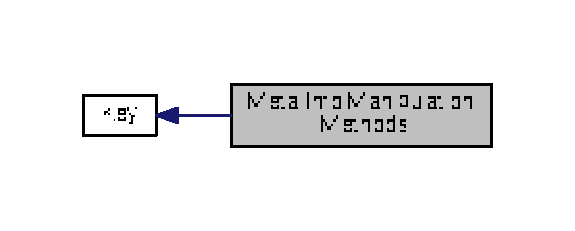
\includegraphics[width=281pt]{group__keymeta}
\end{center}
\end{figure}
\doxysubsection*{Functions}
\begin{DoxyCompactItemize}
\item 
int \mbox{\hyperlink{group__keymeta_ga5dbb669802eea27e106ee3a5e39717a9}{key\+Rewind\+Meta}} (Key $\ast$key)
\begin{DoxyCompactList}\small\item\em Rewind the internal iterator to the first entry in metadata keyset. \end{DoxyCompactList}\item 
const Key $\ast$ \mbox{\hyperlink{group__keymeta_ga4c88342f580a4291455a801af71ce048}{key\+Next\+Meta}} (Key $\ast$key)
\begin{DoxyCompactList}\small\item\em Get the next metadata entry of a Key. \end{DoxyCompactList}\item 
const Key $\ast$ \mbox{\hyperlink{group__keymeta_ga74a273f529030f4947df52e14fdd2869}{key\+Current\+Meta}} (const Key $\ast$key)
\begin{DoxyCompactList}\small\item\em Returns the metadata Key at the internal iterator\textquotesingle{}s current position. \end{DoxyCompactList}\item 
int \mbox{\hyperlink{group__keymeta_ga9a22b992478e613c8788bd460b4a1f0c}{key\+Copy\+Meta}} (Key $\ast$dest, const Key $\ast$source, const char $\ast$meta\+Name)
\begin{DoxyCompactList}\small\item\em Do a shallow copy of metadata with name {\ttfamily meta\+Name} from source to dest. \end{DoxyCompactList}\item 
int \mbox{\hyperlink{group__keymeta_ga8e63720a65610a29597494d0671f9401}{key\+Copy\+All\+Meta}} (Key $\ast$dest, const Key $\ast$source)
\begin{DoxyCompactList}\small\item\em Do a shallow copy of all metadata from source to dest. \end{DoxyCompactList}\item 
const Key $\ast$ \mbox{\hyperlink{group__keymeta_ga9ed3875495ddb3d8a8d29158a60a147c}{key\+Get\+Meta}} (const Key $\ast$key, const char $\ast$meta\+Name)
\begin{DoxyCompactList}\small\item\em Returns the Key for a metadata entry with name {\ttfamily meta\+Name}. \end{DoxyCompactList}\item 
ssize\+\_\+t \mbox{\hyperlink{group__keymeta_gae1f15546b234ffb6007d8a31178652b9}{key\+Set\+Meta}} (Key $\ast$key, const char $\ast$meta\+Name, const char $\ast$new\+Meta\+String)
\begin{DoxyCompactList}\small\item\em Set a new metadata Key. \end{DoxyCompactList}\item 
Key\+Set $\ast$ \mbox{\hyperlink{group__keymeta_ga11706f1753e67933f7cffc5c0345cd29}{key\+Meta}} (Key $\ast$key)
\begin{DoxyCompactList}\small\item\em Returns the Key\+Set holding the given Key\textquotesingle{}s metadata. \end{DoxyCompactList}\end{DoxyCompactItemize}


\doxysubsection{Detailed Description}
Methods to do various operations on Key metadata. 

To use them\+: 
\begin{DoxyCode}{0}
\DoxyCodeLine{\textcolor{preprocessor}{\#include <kdb.h>}}

\end{DoxyCode}


Next to \mbox{\hyperlink{group__keyname}{Name (key and owner) }} and \mbox{\hyperlink{group__keyvalue}{value (data and comment) }} there is the so called meta information inside every key.

Key meta information are an unlimited number of key/value pairs strongly related to a key. It main purpose is to give keys special semantics, so that plugins can treat them differently.

Metakey, as opposed to Key, deliberately has following limitations\+:
\begin{DoxyItemize}
\item no null values
\item no binary data
\item no modification of references (COW)
\item no guarantee of ordering
\end{DoxyItemize}\hypertarget{group__keymeta_autotoc_md0}{}\doxysubsubsection{Examples for metadata}\label{group__keymeta_autotoc_md0}
File system information (see stat(2) for more information)\+:
\begin{DoxyItemize}
\item uid\+: the user id (positive number)
\item gid\+: the group id (positive number)
\item mode\+: filesystem-\/like mode permissions (positive octal number)
\item atime\+: When was the key accessed the last time.
\item mtime\+: When was the key modified the last time.
\item ctime\+: When the uid, gid or mode of a key changes. (times are represented through a positive number as unix timestamp)
\end{DoxyItemize}

The comment can contain userdata which directly belong to that key. The name of the meta information is \char`\"{}comment\char`\"{} for a general purpose comment about the key. Multi-\/\+Language comments are also supported by appending \mbox{[}LANG\mbox{]} to the name.

Validators are regular expressions which are tested against the key value. The metakey \char`\"{}validator\char`\"{} can hold a regular expression which will be matched against.

Types can be expressed with the meta information \char`\"{}type\char`\"{}.

The relevance of the key can be tagged with a value from -\/20 to 20. Negative numbers are the more important and must be present in order to start the program.

A version of a key may be stored with \char`\"{}version\char`\"{}. Its format is full.\+major.\+minor where all of these are integers.

The order inside a persistent storage can be described with the tag \char`\"{}order\char`\"{} which contains a positive number.

The metakey \char`\"{}app\char`\"{} describes to which application a key belongs. It can be used to remove keys from an application no longer installed.

The metakey \char`\"{}path\char`\"{} describes where the key is physically stored.

The \char`\"{}owner\char`\"{} is the user that owns the key. It only works for the user\+:/ hierarchy. It rather says where the key is stored and says nothing about the filesystem properties. 

\doxysubsection{Function Documentation}
\mbox{\Hypertarget{group__keymeta_ga8e63720a65610a29597494d0671f9401}\label{group__keymeta_ga8e63720a65610a29597494d0671f9401}} 
\index{Meta Info Manipulation Methods@{Meta Info Manipulation Methods}!keyCopyAllMeta@{keyCopyAllMeta}}
\index{keyCopyAllMeta@{keyCopyAllMeta}!Meta Info Manipulation Methods@{Meta Info Manipulation Methods}}
\doxysubsubsection{\texorpdfstring{keyCopyAllMeta()}{keyCopyAllMeta()}}
{\footnotesize\ttfamily int key\+Copy\+All\+Meta (\begin{DoxyParamCaption}\item[{Key $\ast$}]{dest,  }\item[{const Key $\ast$}]{source }\end{DoxyParamCaption})}



Do a shallow copy of all metadata from source to dest. 

The key dest will additionally have all metadata the source had. Metadata not present in source will not be changed. Metadata which was present in source and dest will be overwritten. If the {\ttfamily dest} Key is read-\/only it will not be changed.

For example the metadata type is copied into the Key k\+:


\begin{DoxyCodeInclude}{0}
\DoxyCodeLine{\textcolor{keywordtype}{void} l (Key * k)}
\DoxyCodeLine{\{}
\DoxyCodeLine{        \textcolor{comment}{// receive copy}}
\DoxyCodeLine{        \mbox{\hyperlink{group__keymeta_ga8e63720a65610a29597494d0671f9401}{keyCopyAllMeta}} (k, copy);}
\DoxyCodeLine{        \textcolor{comment}{// the caller will see the changed key k}}
\DoxyCodeLine{        \textcolor{comment}{// with all the metadata from copy}}
\DoxyCodeLine{\}}

\end{DoxyCodeInclude}
 The main purpose of this function is for plugins or applications which want to add the same metadata to n keys. When you do that with \mbox{\hyperlink{group__keymeta_gae1f15546b234ffb6007d8a31178652b9}{key\+Set\+Meta()}} it will take n times the memory for the key. This can be considerable amount of memory for many keys with some metadata for each.

To avoid that problem you can use \mbox{\hyperlink{group__keymeta_ga8e63720a65610a29597494d0671f9401}{key\+Copy\+All\+Meta()}} or \mbox{\hyperlink{group__keymeta_ga9a22b992478e613c8788bd460b4a1f0c}{key\+Copy\+Meta()}}\+:


\begin{DoxyCodeInclude}{0}
\DoxyCodeLine{\textcolor{keywordtype}{void} o (KeySet * ks)}
\DoxyCodeLine{\{}
\DoxyCodeLine{        Key * current;}
\DoxyCodeLine{        Key * shared = \mbox{\hyperlink{group__key_gad23c65b44bf48d773759e1f9a4d43b89}{keyNew}} (\textcolor{stringliteral}{"{}/"{}}, \mbox{\hyperlink{group__key_gga9b703ca49f48b482def322b77d3e6bc8aa8adb6fcb92dec58fb19410eacfdd403}{KEY\_END}});}
\DoxyCodeLine{        \mbox{\hyperlink{group__keymeta_gae1f15546b234ffb6007d8a31178652b9}{keySetMeta}} (shared, \textcolor{stringliteral}{"{}shared1"{}}, \textcolor{stringliteral}{"{}this metadata should be shared among many keys"{}});}
\DoxyCodeLine{        \mbox{\hyperlink{group__keymeta_gae1f15546b234ffb6007d8a31178652b9}{keySetMeta}} (shared, \textcolor{stringliteral}{"{}shared2"{}}, \textcolor{stringliteral}{"{}this metadata should be shared among many keys also"{}});}
\DoxyCodeLine{        \mbox{\hyperlink{group__keymeta_gae1f15546b234ffb6007d8a31178652b9}{keySetMeta}} (shared, \textcolor{stringliteral}{"{}shared3"{}}, \textcolor{stringliteral}{"{}this metadata should be shared among many keys too"{}});}
\DoxyCodeLine{}
\DoxyCodeLine{        \mbox{\hyperlink{group__keyset_gabe793ff51f1728e3429c84a8a9086b70}{ksRewind}} (ks);}
\DoxyCodeLine{        \textcolor{keywordflow}{while} ((current = \mbox{\hyperlink{group__keyset_ga317321c9065b5a4b3e33fe1c399bcec9}{ksNext}} (ks)) != 0)}
\DoxyCodeLine{        \{}
\DoxyCodeLine{                \textcolor{keywordflow}{if} (needsSharedData (current)) \mbox{\hyperlink{group__keymeta_ga8e63720a65610a29597494d0671f9401}{keyCopyAllMeta}} (current, shared);}
\DoxyCodeLine{        \}}
\DoxyCodeLine{}
\DoxyCodeLine{        \mbox{\hyperlink{group__key_ga3df95bbc2494e3e6703ece5639be5bb1}{keyDel}} (shared);}
\DoxyCodeLine{\}}

\end{DoxyCodeInclude}
 \begin{DoxyPrecond}{Precondition}
{\ttfamily dest\textquotesingle{}s} metadata is not read-\/only 
\end{DoxyPrecond}
\begin{DoxyPostcond}{Postcondition}
for every meta\+Name present in source\+: key\+Get\+Meta(source, meta\+Name) == key\+Get\+Meta(dest, meta\+Name)
\end{DoxyPostcond}

\begin{DoxyParams}{Parameters}
{\em dest} & the destination where the metadata should be copied too \\
\hline
{\em source} & the key where the metadata should be copied from\\
\hline
\end{DoxyParams}

\begin{DoxyRetVals}{Return values}
{\em 1} & if metadata was successfully copied \\
\hline
{\em 0} & if source did not have any metadata \\
\hline
{\em -\/1} & on null pointer of dest or source \\
\hline
{\em -\/1} & on memory problems\\
\hline
\end{DoxyRetVals}
\begin{DoxySince}{Since}
1.\+0.\+0
\end{DoxySince}
\begin{DoxySeeAlso}{See also}
\mbox{\hyperlink{group__keymeta_ga9a22b992478e613c8788bd460b4a1f0c}{key\+Copy\+Meta()}} for copying one metadata Key from {\ttfamily dest} to {\ttfamily source} 
\end{DoxySeeAlso}
\mbox{\Hypertarget{group__keymeta_ga9a22b992478e613c8788bd460b4a1f0c}\label{group__keymeta_ga9a22b992478e613c8788bd460b4a1f0c}} 
\index{Meta Info Manipulation Methods@{Meta Info Manipulation Methods}!keyCopyMeta@{keyCopyMeta}}
\index{keyCopyMeta@{keyCopyMeta}!Meta Info Manipulation Methods@{Meta Info Manipulation Methods}}
\doxysubsubsection{\texorpdfstring{keyCopyMeta()}{keyCopyMeta()}}
{\footnotesize\ttfamily int key\+Copy\+Meta (\begin{DoxyParamCaption}\item[{Key $\ast$}]{dest,  }\item[{const Key $\ast$}]{source,  }\item[{const char $\ast$}]{meta\+Name }\end{DoxyParamCaption})}



Do a shallow copy of metadata with name {\ttfamily meta\+Name} from source to dest. 

Afterwards {\ttfamily source} and {\ttfamily dest} will have the same metadata referred with {\ttfamily meta\+Name}. If the Key with name {\ttfamily meta\+Name} doesn\textquotesingle{}t exist in {\ttfamily source} -\/ it gets deleted in {\ttfamily dest}.

For example the metadata type is copied into the Key k.


\begin{DoxyCode}{0}
\DoxyCodeLine{\textcolor{keywordtype}{void} l(Key *k)}
\DoxyCodeLine{\{}
\DoxyCodeLine{        \textcolor{comment}{// receive c}}
\DoxyCodeLine{        \mbox{\hyperlink{group__keymeta_ga9a22b992478e613c8788bd460b4a1f0c}{keyCopyMeta}}(k, c, \textcolor{stringliteral}{"{}type"{}});}
\DoxyCodeLine{        \textcolor{comment}{// the caller will see the changed key k}}
\DoxyCodeLine{        \textcolor{comment}{// with the metadata "{}type"{} from c}}
\DoxyCodeLine{\}}

\end{DoxyCode}


The main purpose of this function is for plugins or applications, which want to add the same metadata to n keys. When you do that \mbox{\hyperlink{group__keymeta_gae1f15546b234ffb6007d8a31178652b9}{key\+Set\+Meta()}} will take n times the memory for the key. This can be a considerable amount of memory for many keys with some metadata for each.

To avoid that problem you can use \mbox{\hyperlink{group__keymeta_ga8e63720a65610a29597494d0671f9401}{key\+Copy\+All\+Meta()}} or \mbox{\hyperlink{group__keymeta_ga9a22b992478e613c8788bd460b4a1f0c}{key\+Copy\+Meta()}}.


\begin{DoxyCode}{0}
\DoxyCodeLine{\textcolor{keywordtype}{void} o(KeySet *ks)}
\DoxyCodeLine{\{}
\DoxyCodeLine{        Key *current;}
\DoxyCodeLine{        Key *shared = \mbox{\hyperlink{group__key_gad23c65b44bf48d773759e1f9a4d43b89}{keyNew}} (\textcolor{stringliteral}{"{}/"{}}, \mbox{\hyperlink{group__key_gga9b703ca49f48b482def322b77d3e6bc8aa8adb6fcb92dec58fb19410eacfdd403}{KEY\_END}});}
\DoxyCodeLine{        \mbox{\hyperlink{group__keymeta_gae1f15546b234ffb6007d8a31178652b9}{keySetMeta}}(shared, \textcolor{stringliteral}{"{}shared"{}}, \textcolor{stringliteral}{"{}this metadata should be shared among many keys"{}});}
\DoxyCodeLine{}
\DoxyCodeLine{        \mbox{\hyperlink{group__keyset_gabe793ff51f1728e3429c84a8a9086b70}{ksRewind}}(ks);}
\DoxyCodeLine{        \textcolor{keywordflow}{while} ((current = \mbox{\hyperlink{group__keyset_ga317321c9065b5a4b3e33fe1c399bcec9}{ksNext}}(ks)) != 0)}
\DoxyCodeLine{        \{}
\DoxyCodeLine{                \textcolor{keywordflow}{if} (needs\_shared\_data(current)) \mbox{\hyperlink{group__keymeta_ga9a22b992478e613c8788bd460b4a1f0c}{keyCopyMeta}}(current, shared, \textcolor{stringliteral}{"{}shared"{}});}
\DoxyCodeLine{        \}}
\DoxyCodeLine{\}}

\end{DoxyCode}


\begin{DoxyPrecond}{Precondition}
{\ttfamily dest\textquotesingle{}s} metadata is not read-\/only 
\end{DoxyPrecond}
\begin{DoxyPostcond}{Postcondition}
key\+Get\+Meta(source, meta\+Name) == key\+Get\+Meta(dest, meta\+Name)
\end{DoxyPostcond}

\begin{DoxyParams}{Parameters}
{\em dest} & the destination where the metadata should be copied to \\
\hline
{\em source} & the key where the metadata should be copied from \\
\hline
{\em meta\+Name} & the name of the metadata Key which should be copied\\
\hline
\end{DoxyParams}

\begin{DoxyRetVals}{Return values}
{\em 1} & if was successfully copied \\
\hline
{\em 0} & if the metadata in dest was removed too \\
\hline
{\em -\/1} & on null pointers (source or dest) \\
\hline
{\em -\/1} & on memory problems \\
\hline
{\em -\/1} & if metadata is read-\/only\\
\hline
\end{DoxyRetVals}
\begin{DoxySince}{Since}
1.\+0.\+0
\end{DoxySince}
\begin{DoxySeeAlso}{See also}
\mbox{\hyperlink{group__keymeta_ga8e63720a65610a29597494d0671f9401}{key\+Copy\+All\+Meta()}} copies all metadata from {\ttfamily dest} to {\ttfamily src} 
\end{DoxySeeAlso}
\mbox{\Hypertarget{group__keymeta_ga74a273f529030f4947df52e14fdd2869}\label{group__keymeta_ga74a273f529030f4947df52e14fdd2869}} 
\index{Meta Info Manipulation Methods@{Meta Info Manipulation Methods}!keyCurrentMeta@{keyCurrentMeta}}
\index{keyCurrentMeta@{keyCurrentMeta}!Meta Info Manipulation Methods@{Meta Info Manipulation Methods}}
\doxysubsubsection{\texorpdfstring{keyCurrentMeta()}{keyCurrentMeta()}}
{\footnotesize\ttfamily const Key$\ast$ key\+Current\+Meta (\begin{DoxyParamCaption}\item[{const Key $\ast$}]{key }\end{DoxyParamCaption})}



Returns the metadata Key at the internal iterator\textquotesingle{}s current position. 

The returned pointer is NULL if the end has been reached or after calling \mbox{\hyperlink{group__keyset_gabe793ff51f1728e3429c84a8a9086b70}{ks\+Rewind()}}.

\begin{DoxyNote}{Note}
You must not delete or change the returned key, use \mbox{\hyperlink{group__keymeta_gae1f15546b234ffb6007d8a31178652b9}{key\+Set\+Meta()}} if you want to delete or change it.
\end{DoxyNote}

\begin{DoxyParams}{Parameters}
{\em key} & Key to get the current metadata from\\
\hline
\end{DoxyParams}
\begin{DoxyReturn}{Returns}
a buffer to the value pointed by {\ttfamily key\textquotesingle{}s} cursor 
\end{DoxyReturn}

\begin{DoxyRetVals}{Return values}
{\em 0} & on NULL pointer\\
\hline
\end{DoxyRetVals}
\begin{DoxySince}{Since}
1.\+0.\+0
\end{DoxySince}
\begin{DoxySeeAlso}{See also}
\mbox{\hyperlink{group__keymeta_ga4c88342f580a4291455a801af71ce048}{key\+Next\+Meta()}} for getting the next value 

\mbox{\hyperlink{group__keymeta_ga5dbb669802eea27e106ee3a5e39717a9}{key\+Rewind\+Meta()}} for rewinding the internal iterator 

\mbox{\hyperlink{group__keyset_ga4287b9416912c5f2ab9c195cb74fb094}{ks\+Current()}} Key\+Sets\textquotesingle{}s equivalent function for getting the current Key 
\end{DoxySeeAlso}
\mbox{\Hypertarget{group__keymeta_ga9ed3875495ddb3d8a8d29158a60a147c}\label{group__keymeta_ga9ed3875495ddb3d8a8d29158a60a147c}} 
\index{Meta Info Manipulation Methods@{Meta Info Manipulation Methods}!keyGetMeta@{keyGetMeta}}
\index{keyGetMeta@{keyGetMeta}!Meta Info Manipulation Methods@{Meta Info Manipulation Methods}}
\doxysubsubsection{\texorpdfstring{keyGetMeta()}{keyGetMeta()}}
{\footnotesize\ttfamily const Key$\ast$ key\+Get\+Meta (\begin{DoxyParamCaption}\item[{const Key $\ast$}]{key,  }\item[{const char $\ast$}]{meta\+Name }\end{DoxyParamCaption})}



Returns the Key for a metadata entry with name {\ttfamily meta\+Name}. 

You are not allowed to modify the resulting key.

If {\ttfamily meta\+Name} does not start with \textquotesingle{}meta\+:/\textquotesingle{}, it will be prefixed with \textquotesingle{}meta\+:/\textquotesingle{}.


\begin{DoxyCode}{0}
\DoxyCodeLine{Key metaData = \mbox{\hyperlink{group__keymeta_ga9ed3875495ddb3d8a8d29158a60a147c}{keyGetMeta}}(k, \textcolor{stringliteral}{"{}type"{}})}
\DoxyCodeLine{\textcolor{comment}{// keyType == "{}boolean"{}}}
\DoxyCodeLine{char keyType[] = \mbox{\hyperlink{group__keyvalue_ga6f29609c5da53c6dc26a98678d5752af}{keyValue}}(metaData)}

\end{DoxyCode}


\begin{DoxyNote}{Note}
You must not delete or change the returned key, use \mbox{\hyperlink{group__keymeta_gae1f15546b234ffb6007d8a31178652b9}{key\+Set\+Meta()}} if you want to delete or change it.
\end{DoxyNote}
\begin{DoxyPrecond}{Precondition}
{\ttfamily key} contains metadata 

{\ttfamily meta\+Name} is prefixed with \char`\"{}meta\+:/\char`\"{}
\end{DoxyPrecond}

\begin{DoxyParams}{Parameters}
{\em key} & the Key from which to get metadata \\
\hline
{\em meta\+Name} & the name of the meta information you want the Key from.\\
\hline
\end{DoxyParams}
\begin{DoxyReturn}{Returns}
value of meta-\/information if meta-\/information is found 
\end{DoxyReturn}

\begin{DoxyRetVals}{Return values}
{\em 0} & if key or meta\+Name is NULL \\
\hline
{\em 0} & if no such meta\+Name is found\\
\hline
\end{DoxyRetVals}
\begin{DoxySince}{Since}
1.\+0.\+0
\end{DoxySince}
\begin{DoxySeeAlso}{See also}
\mbox{\hyperlink{group__keymeta_gae1f15546b234ffb6007d8a31178652b9}{key\+Set\+Meta()}} for setting metadata 

\mbox{\hyperlink{group__keymeta_ga11706f1753e67933f7cffc5c0345cd29}{key\+Meta()}} for getting the Key\+Set containing metadata 
\end{DoxySeeAlso}
\mbox{\Hypertarget{group__keymeta_ga11706f1753e67933f7cffc5c0345cd29}\label{group__keymeta_ga11706f1753e67933f7cffc5c0345cd29}} 
\index{Meta Info Manipulation Methods@{Meta Info Manipulation Methods}!keyMeta@{keyMeta}}
\index{keyMeta@{keyMeta}!Meta Info Manipulation Methods@{Meta Info Manipulation Methods}}
\doxysubsubsection{\texorpdfstring{keyMeta()}{keyMeta()}}
{\footnotesize\ttfamily Key\+Set$\ast$ key\+Meta (\begin{DoxyParamCaption}\item[{Key $\ast$}]{key }\end{DoxyParamCaption})}



Returns the Key\+Set holding the given Key\textquotesingle{}s metadata. 

Use \mbox{\hyperlink{group__keymeta_gae1f15546b234ffb6007d8a31178652b9}{key\+Set\+Meta()}} to populate the metadata Key\+Set of a Key.


\begin{DoxyCodeInclude}{0}
\DoxyCodeLine{        Key * key = \mbox{\hyperlink{group__key_gad23c65b44bf48d773759e1f9a4d43b89}{keyNew}} (\textcolor{stringliteral}{"{}user:/test/key"{}}, \mbox{\hyperlink{group__key_gga9b703ca49f48b482def322b77d3e6bc8aa8adb6fcb92dec58fb19410eacfdd403}{KEY\_END}});}
\DoxyCodeLine{}
\DoxyCodeLine{        \mbox{\hyperlink{group__keymeta_gae1f15546b234ffb6007d8a31178652b9}{keySetMeta}} (key, \textcolor{stringliteral}{"{}meta1"{}}, \textcolor{stringliteral}{"{}value1"{}});}
\DoxyCodeLine{        \mbox{\hyperlink{group__keymeta_gae1f15546b234ffb6007d8a31178652b9}{keySetMeta}} (key, \textcolor{stringliteral}{"{}meta2"{}}, \textcolor{stringliteral}{"{}value2"{}});}

\end{DoxyCodeInclude}
 Iterate the returned metadata Key\+Set like any other Key\+Set.


\begin{DoxyCodeInclude}{0}
\DoxyCodeLine{        Key * cur;}
\DoxyCodeLine{        \mbox{\hyperlink{group__keyset_gabe793ff51f1728e3429c84a8a9086b70}{ksRewind}} (\mbox{\hyperlink{group__keymeta_ga11706f1753e67933f7cffc5c0345cd29}{keyMeta}} (key));}
\DoxyCodeLine{        \textcolor{keywordflow}{while} ((cur = \mbox{\hyperlink{group__keyset_ga317321c9065b5a4b3e33fe1c399bcec9}{ksNext}} (\mbox{\hyperlink{group__keymeta_ga11706f1753e67933f7cffc5c0345cd29}{keyMeta}} (key))) != NULL)}
\DoxyCodeLine{        \{}
\DoxyCodeLine{                printf (\textcolor{stringliteral}{"{}meta name: \%s, meta value: \%s\(\backslash\)n"{}}, \mbox{\hyperlink{group__keyname_ga8e805c726a60da921d3736cda7813513}{keyName}} (cur), \mbox{\hyperlink{group__keyvalue_ga880936f2481d28e6e2acbe7486a21d05}{keyString}} (cur));}
\DoxyCodeLine{        \}}

\end{DoxyCodeInclude}
 Use \mbox{\hyperlink{group__keyset_ga60f1ddcf23272f2b29b90e92ebe9b56f}{ks\+Lookup()}} or \mbox{\hyperlink{group__keymeta_ga9ed3875495ddb3d8a8d29158a60a147c}{key\+Get\+Meta()}} to retrieve a single value for a given Key.


\begin{DoxyCodeInclude}{0}
\DoxyCodeLine{        Key * lookupKey = \mbox{\hyperlink{group__keyset_gad65d2cdcbb5381194a1688e169af8a83}{ksLookupByName}} (\mbox{\hyperlink{group__keymeta_ga11706f1753e67933f7cffc5c0345cd29}{keyMeta}} (key), \textcolor{stringliteral}{"{}meta2"{}}, 0);}
\DoxyCodeLine{        printf (\textcolor{stringliteral}{"{}meta name: \%s, meta value: \%s\(\backslash\)n"{}}, \mbox{\hyperlink{group__keyname_ga8e805c726a60da921d3736cda7813513}{keyName}} (lookupKey), \mbox{\hyperlink{group__keyvalue_ga880936f2481d28e6e2acbe7486a21d05}{keyString}} (lookupKey));}
\DoxyCodeLine{        \mbox{\hyperlink{group__key_ga3df95bbc2494e3e6703ece5639be5bb1}{keyDel}} (key);}

\end{DoxyCodeInclude}
 \begin{DoxyNote}{Note}
You are not allowed to modify the name of Key\+Set\textquotesingle{}s Keys or delete them. 

You must not delete the returned Key\+Set. 

Adding a key with metadata to the Key\+Set is an error.
\end{DoxyNote}
\begin{DoxyPostcond}{Postcondition}
for the returned Key\+Set ks\+: key\+Get\+Meta(key, meta\+Name) == ks\+Lookup\+By\+Name(ks, meta\+Name) 

{\ttfamily key} contains a Key\+Set for the metadata
\end{DoxyPostcond}

\begin{DoxyParams}{Parameters}
{\em key} & the Key from which to get the metadata Key\+Set\\
\hline
\end{DoxyParams}
\begin{DoxyReturn}{Returns}
the Key\+Set holding the metadata 
\end{DoxyReturn}

\begin{DoxyRetVals}{Return values}
{\em 0} & if the Key is 0 \\
\hline
{\em 0} & if the Key has no metadata\\
\hline
\end{DoxyRetVals}
\begin{DoxySince}{Since}
1.\+0.\+0
\end{DoxySince}
\begin{DoxySeeAlso}{See also}
\mbox{\hyperlink{group__keymeta_gae1f15546b234ffb6007d8a31178652b9}{key\+Set\+Meta()}} for setting a metadata Key 

\mbox{\hyperlink{group__keymeta_ga9ed3875495ddb3d8a8d29158a60a147c}{key\+Get\+Meta()}} for getting a metadata Key 
\end{DoxySeeAlso}
\mbox{\Hypertarget{group__keymeta_ga4c88342f580a4291455a801af71ce048}\label{group__keymeta_ga4c88342f580a4291455a801af71ce048}} 
\index{Meta Info Manipulation Methods@{Meta Info Manipulation Methods}!keyNextMeta@{keyNextMeta}}
\index{keyNextMeta@{keyNextMeta}!Meta Info Manipulation Methods@{Meta Info Manipulation Methods}}
\doxysubsubsection{\texorpdfstring{keyNextMeta()}{keyNextMeta()}}
{\footnotesize\ttfamily const Key$\ast$ key\+Next\+Meta (\begin{DoxyParamCaption}\item[{Key $\ast$}]{key }\end{DoxyParamCaption})}



Get the next metadata entry of a Key. 

Keys have an internal cursor that can be reset with \mbox{\hyperlink{group__keymeta_ga5dbb669802eea27e106ee3a5e39717a9}{key\+Rewind\+Meta()}}. Every time \mbox{\hyperlink{group__keymeta_ga4c88342f580a4291455a801af71ce048}{key\+Next\+Meta()}} is called the cursor is incremented and the new current Name of Meta Information is returned.

You\textquotesingle{}ll get a NULL pointer if the metadata after the end of the Key was reached. On subsequent calls of \mbox{\hyperlink{group__keymeta_ga4c88342f580a4291455a801af71ce048}{key\+Next\+Meta()}} it will still return the NULL pointer.

The {\ttfamily key} internal cursor will be changed, so it is not const.

\begin{DoxyNote}{Note}
That the resulting key is guaranteed to have a value, because meta information has no binary or null pointer semantics.

You must not delete or change the returned key, use \mbox{\hyperlink{group__keymeta_gae1f15546b234ffb6007d8a31178652b9}{key\+Set\+Meta()}} if you want to delete or change it.
\end{DoxyNote}

\begin{DoxyParams}{Parameters}
{\em key} & the Key object to work with\\
\hline
\end{DoxyParams}
\begin{DoxyReturn}{Returns}
a key containing metadata 
\end{DoxyReturn}

\begin{DoxyRetVals}{Return values}
{\em 0} & when the last Key has been reached \\
\hline
{\em 0} & when Key is a NULL pointer\\
\hline
\end{DoxyRetVals}
\begin{DoxySince}{Since}
1.\+0.\+0
\end{DoxySince}
\begin{DoxySeeAlso}{See also}
\mbox{\hyperlink{group__keyset_ga317321c9065b5a4b3e33fe1c399bcec9}{ks\+Next()}} for pedant in iterator interface of Key\+Set 

\mbox{\hyperlink{group__keymeta_ga5dbb669802eea27e106ee3a5e39717a9}{key\+Rewind\+Meta()}} for rewinding the internal iterator 

\mbox{\hyperlink{group__keymeta_ga74a273f529030f4947df52e14fdd2869}{key\+Current\+Meta()}} for getting the current metadata Key 
\end{DoxySeeAlso}
\mbox{\Hypertarget{group__keymeta_ga5dbb669802eea27e106ee3a5e39717a9}\label{group__keymeta_ga5dbb669802eea27e106ee3a5e39717a9}} 
\index{Meta Info Manipulation Methods@{Meta Info Manipulation Methods}!keyRewindMeta@{keyRewindMeta}}
\index{keyRewindMeta@{keyRewindMeta}!Meta Info Manipulation Methods@{Meta Info Manipulation Methods}}
\doxysubsubsection{\texorpdfstring{keyRewindMeta()}{keyRewindMeta()}}
{\footnotesize\ttfamily int key\+Rewind\+Meta (\begin{DoxyParamCaption}\item[{Key $\ast$}]{key }\end{DoxyParamCaption})}



Rewind the internal iterator to the first entry in metadata keyset. 

Use this function to set the cursor to the beginning of the Key Meta Infos. \mbox{\hyperlink{group__keymeta_ga74a273f529030f4947df52e14fdd2869}{key\+Current\+Meta()}} will always return NULL after rewinding, so you need to call \mbox{\hyperlink{group__keymeta_ga4c88342f580a4291455a801af71ce048}{key\+Next\+Meta()}} first.


\begin{DoxyCode}{0}
\DoxyCodeLine{Key *key;}
\DoxyCodeLine{\textcolor{keyword}{const} Key *meta;}
\DoxyCodeLine{}
\DoxyCodeLine{\mbox{\hyperlink{group__keymeta_ga5dbb669802eea27e106ee3a5e39717a9}{keyRewindMeta}} (key);}
\DoxyCodeLine{\textcolor{keywordflow}{while} ((meta = \mbox{\hyperlink{group__keymeta_ga4c88342f580a4291455a801af71ce048}{keyNextMeta}} (key))!=0)}
\DoxyCodeLine{\{}
\DoxyCodeLine{        printf (\textcolor{stringliteral}{"{}name: \%s, value: \%s"{}}, \mbox{\hyperlink{group__keyname_ga8e805c726a60da921d3736cda7813513}{keyName}}(meta), \mbox{\hyperlink{group__keyvalue_ga880936f2481d28e6e2acbe7486a21d05}{keyString}}(meta));}
\DoxyCodeLine{\}}

\end{DoxyCode}



\begin{DoxyParams}{Parameters}
{\em key} & Key whose internal iterator should be rewinded\\
\hline
\end{DoxyParams}

\begin{DoxyRetVals}{Return values}
{\em 0} & on success \\
\hline
{\em 0} & if there is no metadata for that key (\mbox{\hyperlink{group__keymeta_ga4c88342f580a4291455a801af71ce048}{key\+Next\+Meta()}} will always return 0 in that case) \\
\hline
{\em -\/1} & on NULL pointer\\
\hline
\end{DoxyRetVals}
\begin{DoxySince}{Since}
1.\+0.\+0
\end{DoxySince}
\begin{DoxySeeAlso}{See also}
\mbox{\hyperlink{group__keymeta_ga4c88342f580a4291455a801af71ce048}{key\+Next\+Meta()}}, \mbox{\hyperlink{group__keymeta_ga74a273f529030f4947df52e14fdd2869}{key\+Current\+Meta()}} for iterating after rewinding 

\mbox{\hyperlink{group__keyset_gabe793ff51f1728e3429c84a8a9086b70}{ks\+Rewind()}} Key\+Set\textquotesingle{}s equivalent function for rewinding 
\end{DoxySeeAlso}
\mbox{\Hypertarget{group__keymeta_gae1f15546b234ffb6007d8a31178652b9}\label{group__keymeta_gae1f15546b234ffb6007d8a31178652b9}} 
\index{Meta Info Manipulation Methods@{Meta Info Manipulation Methods}!keySetMeta@{keySetMeta}}
\index{keySetMeta@{keySetMeta}!Meta Info Manipulation Methods@{Meta Info Manipulation Methods}}
\doxysubsubsection{\texorpdfstring{keySetMeta()}{keySetMeta()}}
{\footnotesize\ttfamily ssize\+\_\+t key\+Set\+Meta (\begin{DoxyParamCaption}\item[{Key $\ast$}]{key,  }\item[{const char $\ast$}]{meta\+Name,  }\item[{const char $\ast$}]{new\+Meta\+String }\end{DoxyParamCaption})}



Set a new metadata Key. 

Will set a new metadata pair with name {\ttfamily meta\+Name} and value {\ttfamily new\+Meta\+String}.

Will add a new metadata Key, if {\ttfamily meta\+Name} was unused until now.

It will modify an existing Pair of metadata if {\ttfamily meta\+Name} was already present.

It will remove a metadata Key if {\ttfamily new\+Meta\+String} is 0.

If {\ttfamily meta\+Name} does not start with \textquotesingle{}meta\+:/\textquotesingle{}, it will be prefixed with \textquotesingle{}meta\+:/\textquotesingle{}.

\begin{DoxyPrecond}{Precondition}
{\ttfamily meta\+Name} is prefixed with \char`\"{}meta\+:/\char`\"{} 

{\ttfamily key\textquotesingle{}s} metadata is not read-\/only 
\end{DoxyPrecond}
\begin{DoxyPostcond}{Postcondition}
The value in {\ttfamily key\textquotesingle{}s} metadata Keyset for {\ttfamily meta\+Name} is {\ttfamily new\+Meta\+String} 
\end{DoxyPostcond}

\begin{DoxyParams}{Parameters}
{\em key} & Key whose metadata should be set \\
\hline
{\em meta\+Name} & name of the metadata Key that should be set \\
\hline
{\em new\+Meta\+String} & new value for the metadata Key\\
\hline
\end{DoxyParams}
\begin{DoxyReturn}{Returns}
size ($>$0) of {\ttfamily new\+Meta\+String} if metadata has been successfully added 
\end{DoxyReturn}

\begin{DoxyRetVals}{Return values}
{\em 0} & if the meta-\/information for meta\+Name was removed \\
\hline
{\em -\/1} & if key or meta\+Name is 0 \\
\hline
{\em -\/1} & if system is out of memory \\
\hline
{\em -\/1} & if {\ttfamily meta\+Name} is not a valid metadata name\\
\hline
\end{DoxyRetVals}
\begin{DoxySince}{Since}
1.\+0.\+0
\end{DoxySince}
\begin{DoxySeeAlso}{See also}
\mbox{\hyperlink{group__keymeta_ga9ed3875495ddb3d8a8d29158a60a147c}{key\+Get\+Meta()}} for getting the value of a metadata Key 

\mbox{\hyperlink{group__keymeta_ga11706f1753e67933f7cffc5c0345cd29}{key\+Meta()}} for getting the Key\+Set containing metadata 
\end{DoxySeeAlso}

\hypertarget{group__keytest}{}\section{Methods for Making Tests}
\label{group__keytest}\index{Methods for Making Tests@{Methods for Making Tests}}


Methods to do various tests on Keys.  


Collaboration diagram for Methods for Making Tests\+:
\nopagebreak
\begin{figure}[H]
\begin{center}
\leavevmode
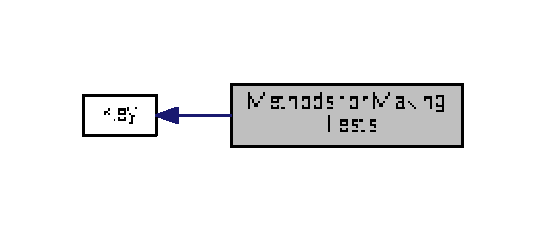
\includegraphics[width=253pt]{group__keytest}
\end{center}
\end{figure}
\subsection*{Functions}
\begin{DoxyCompactItemize}
\item 
int \hyperlink{group__keytest_gaf6e66e12fe04d535a5d1c8218ced803e}{key\+Cmp} (const Key $\ast$k1, const Key $\ast$k2)
\begin{DoxyCompactList}\small\item\em Compare the name of two keys. \end{DoxyCompactList}\item 
int \hyperlink{group__keytest_gaf247df0de7aca04b32ef80e39ef12950}{key\+Need\+Sync} (const Key $\ast$key)
\begin{DoxyCompactList}\small\item\em Test if a key needs to be synced to backend storage. \end{DoxyCompactList}\item 
int \hyperlink{group__keytest_ga03332b5d97c76a4fd2640aca4762b8df}{key\+Is\+Below} (const Key $\ast$key, const Key $\ast$check)
\begin{DoxyCompactList}\small\item\em Check if the key check is below the key key or not. \end{DoxyCompactList}\item 
int \hyperlink{group__keytest_ga0150fb549225d8789e7297b919965e72}{key\+Is\+Directly\+Below} (const Key $\ast$key, const Key $\ast$check)
\begin{DoxyCompactList}\small\item\em Check whether the key {\ttfamily check} is directly below the key {\ttfamily key}. \end{DoxyCompactList}\item 
int \hyperlink{group__keytest_gaa25f699f592031c1a0abc1504d14e13e}{key\+Is\+Inactive} (const Key $\ast$key)
\begin{DoxyCompactList}\small\item\em Check whether a key is inactive. \end{DoxyCompactList}\item 
int \hyperlink{group__keytest_ga9526b371087564e43e3dff8ad0dac949}{key\+Is\+Binary} (const Key $\ast$key)
\begin{DoxyCompactList}\small\item\em Check if a key is binary type. \end{DoxyCompactList}\item 
int \hyperlink{group__keytest_gaea7670778abd07fee0fe8ac12a149190}{key\+Is\+String} (const Key $\ast$key)
\begin{DoxyCompactList}\small\item\em Check if a key is string type. \end{DoxyCompactList}\end{DoxyCompactItemize}


\subsection{Detailed Description}
Methods to do various tests on Keys. 

To use them\+: 
\begin{DoxyCode}
\textcolor{preprocessor}{#include <kdb.h>}
\end{DoxyCode}
 

\subsection{Function Documentation}
\mbox{\Hypertarget{group__keytest_gaf6e66e12fe04d535a5d1c8218ced803e}\label{group__keytest_gaf6e66e12fe04d535a5d1c8218ced803e}} 
\index{Methods for Making Tests@{Methods for Making Tests}!key\+Cmp@{key\+Cmp}}
\index{key\+Cmp@{key\+Cmp}!Methods for Making Tests@{Methods for Making Tests}}
\subsubsection{\texorpdfstring{key\+Cmp()}{keyCmp()}}
{\footnotesize\ttfamily int key\+Cmp (\begin{DoxyParamCaption}\item[{const Key $\ast$}]{k1,  }\item[{const Key $\ast$}]{k2 }\end{DoxyParamCaption})}



Compare the name of two keys. 

\begin{DoxyReturn}{Returns}
a number less than, equal to or greater than zero if k1 is found, respectively, to be less than, to match, or be greater than k2.
\end{DoxyReturn}
The comparison is based on a strcmp of the keynames, and iff they match a strcmp of the owner will be used to distuingish. If even this matches the keys are found to be exactly the same and 0 is returned. These two keys can\textquotesingle{}t be used in the same Key\+Set.

\hyperlink{group__keytest_gaf6e66e12fe04d535a5d1c8218ced803e}{key\+Cmp()} defines the sorting order for a Key\+Set.

The following 3 points are the rules for null values\+:


\begin{DoxyItemize}
\item A null pointer will be found to be smaller than every other key. If both are null pointers, 0 is returned.
\item A null name will be found to be smaller than every other name. If both are null names, 0 is returned.
\end{DoxyItemize}

If the name is equal then\+:


\begin{DoxyItemize}
\item No owner will be found to be smaller then every other owner. If both don\textquotesingle{}t have an owner, 0 is returned.
\end{DoxyItemize}

\begin{DoxyNote}{Note}
the owner will only be used if the names are equal.
\end{DoxyNote}
Given any Keys k1 and k2 constructed with \hyperlink{group__key_gad23c65b44bf48d773759e1f9a4d43b89}{key\+New()}, following equation hold true\+:


\begin{DoxyCodeInclude}
        succeed\_if (\hyperlink{group__keytest_gaf6e66e12fe04d535a5d1c8218ced803e}{keyCmp} (0, 0) == 0, \textcolor{stringliteral}{"all null pointers same"});
        succeed\_if (\hyperlink{group__keytest_gaf6e66e12fe04d535a5d1c8218ced803e}{keyCmp} (k1, 0) == 1, \textcolor{stringliteral}{"null pointer is smaller"});
        succeed\_if (\hyperlink{group__keytest_gaf6e66e12fe04d535a5d1c8218ced803e}{keyCmp} (0, k2) == -1, \textcolor{stringliteral}{"null pointer is smaller"});
\end{DoxyCodeInclude}
 Here are some more examples\+: 
\begin{DoxyCode}
Key *k1 = \hyperlink{group__key_gad23c65b44bf48d773759e1f9a4d43b89}{keyNew}(\textcolor{stringliteral}{"user/a"}, \hyperlink{group__key_gga9b703ca49f48b482def322b77d3e6bc8aa8adb6fcb92dec58fb19410eacfdd403}{KEY\_END});
Key *k2 = \hyperlink{group__key_gad23c65b44bf48d773759e1f9a4d43b89}{keyNew}(\textcolor{stringliteral}{"user/b"}, \hyperlink{group__key_gga9b703ca49f48b482def322b77d3e6bc8aa8adb6fcb92dec58fb19410eacfdd403}{KEY\_END});

\textcolor{comment}{// keyCmp(k1,k2) < 0}
\textcolor{comment}{// keyCmp(k2,k1) > 0}
\end{DoxyCode}


And even more\+: 
\begin{DoxyCode}
Key *k1 = \hyperlink{group__key_gad23c65b44bf48d773759e1f9a4d43b89}{keyNew}(\textcolor{stringliteral}{"user/a"}, \hyperlink{group__key_gga9b703ca49f48b482def322b77d3e6bc8a77ca60362fa8daca8d5347db4385068b}{KEY\_OWNER}, \textcolor{stringliteral}{"markus"}, \hyperlink{group__key_gga9b703ca49f48b482def322b77d3e6bc8aa8adb6fcb92dec58fb19410eacfdd403}{KEY\_END});
Key *k2 = \hyperlink{group__key_gad23c65b44bf48d773759e1f9a4d43b89}{keyNew}(\textcolor{stringliteral}{"user/a"}, \hyperlink{group__key_gga9b703ca49f48b482def322b77d3e6bc8a77ca60362fa8daca8d5347db4385068b}{KEY\_OWNER}, \textcolor{stringliteral}{"max"}, \hyperlink{group__key_gga9b703ca49f48b482def322b77d3e6bc8aa8adb6fcb92dec58fb19410eacfdd403}{KEY\_END});

\textcolor{comment}{// keyCmp(k1,k2) < 0}
\textcolor{comment}{// keyCmp(k2,k1) > 0}
\end{DoxyCode}


Do not strcmp the \hyperlink{group__keyname_ga8e805c726a60da921d3736cda7813513}{key\+Name()} yourself because the result differs from simple ascii comparison.


\begin{DoxyParams}{Parameters}
{\em k1} & the first key object to compare with \\
\hline
{\em k2} & the second key object to compare with\\
\hline
\end{DoxyParams}
\begin{DoxySeeAlso}{See also}
\hyperlink{group__keyset_gaa5a1d467a4d71041edce68ea7748ce45}{ks\+Append\+Key()}, \hyperlink{group__keyset_ga21eb9c3a14a604ee3a8bdc779232e7b7}{ks\+Append()} will compare keys when appending 

\hyperlink{group__keyset_ga60f1ddcf23272f2b29b90e92ebe9b56f}{ks\+Lookup()} will compare keys during searching 
\end{DoxySeeAlso}
\mbox{\Hypertarget{group__keytest_ga03332b5d97c76a4fd2640aca4762b8df}\label{group__keytest_ga03332b5d97c76a4fd2640aca4762b8df}} 
\index{Methods for Making Tests@{Methods for Making Tests}!key\+Is\+Below@{key\+Is\+Below}}
\index{key\+Is\+Below@{key\+Is\+Below}!Methods for Making Tests@{Methods for Making Tests}}
\subsubsection{\texorpdfstring{key\+Is\+Below()}{keyIsBelow()}}
{\footnotesize\ttfamily int key\+Is\+Below (\begin{DoxyParamCaption}\item[{const Key $\ast$}]{key,  }\item[{const Key $\ast$}]{check }\end{DoxyParamCaption})}



Check if the key check is below the key key or not. 

Example\+: \begin{DoxyVerb}key user/sw/app
check user/sw/app/key
\end{DoxyVerb}


returns true because check is below key

Example\+: \begin{DoxyVerb}key user/sw/app
check user/sw/app/folder/key
\end{DoxyVerb}


returns also true because check is indirect below key

Obviously, there is no key above a namespace (e.\+g. user, system, /)\+:

\begin{DoxyVerb}key *
check user
\end{DoxyVerb}



\begin{DoxyParams}{Parameters}
{\em key} & the key object to work with \\
\hline
{\em check} & the key to find the relative position of \\
\hline
\end{DoxyParams}

\begin{DoxyRetVals}{Return values}
{\em 1} & if check is below key \\
\hline
{\em 0} & if it is not below or if it is the same key \\
\hline
{\em -\/1} & if key or check is null \\
\hline
\end{DoxyRetVals}
\begin{DoxySeeAlso}{See also}
\hyperlink{group__keyname_ga7699091610e7f3f43d2949514a4b35d9}{key\+Set\+Name()}, \hyperlink{group__keyname_gab29a850168d9b31c9529e90cf9ab68be}{key\+Get\+Name()}, \hyperlink{group__keytest_ga0150fb549225d8789e7297b919965e72}{key\+Is\+Directly\+Below()} 
\end{DoxySeeAlso}
\mbox{\Hypertarget{group__keytest_ga9526b371087564e43e3dff8ad0dac949}\label{group__keytest_ga9526b371087564e43e3dff8ad0dac949}} 
\index{Methods for Making Tests@{Methods for Making Tests}!key\+Is\+Binary@{key\+Is\+Binary}}
\index{key\+Is\+Binary@{key\+Is\+Binary}!Methods for Making Tests@{Methods for Making Tests}}
\subsubsection{\texorpdfstring{key\+Is\+Binary()}{keyIsBinary()}}
{\footnotesize\ttfamily int key\+Is\+Binary (\begin{DoxyParamCaption}\item[{const Key $\ast$}]{key }\end{DoxyParamCaption})}



Check if a key is binary type. 

The function checks if the key is a binary. Opposed to string values binary values can have \textquotesingle{}\textbackslash{}0\textquotesingle{} inside the value and may not be terminated by a null character. Their disadvantage is that you need to pass their size.

Make sure to use this function and don\textquotesingle{}t test the binary type another way to ensure compatibility and to write less error prone programs.


\begin{DoxyRetVals}{Return values}
{\em 1} & if it is binary \\
\hline
{\em 0} & if it is not \\
\hline
{\em -\/1} & on N\+U\+LL pointer \\
\hline
\end{DoxyRetVals}
\begin{DoxySeeAlso}{See also}
\hyperlink{group__keyvalue_ga4c0d8a4a11174197699c231e0b5c3c84}{key\+Get\+Binary()}, \hyperlink{group__keyvalue_gaa50a5358fd328d373a45f395fa1b99e7}{key\+Set\+Binary()} 
\end{DoxySeeAlso}

\begin{DoxyParams}{Parameters}
{\em key} & the key to check \\
\hline
\end{DoxyParams}
\mbox{\Hypertarget{group__keytest_ga0150fb549225d8789e7297b919965e72}\label{group__keytest_ga0150fb549225d8789e7297b919965e72}} 
\index{Methods for Making Tests@{Methods for Making Tests}!key\+Is\+Directly\+Below@{key\+Is\+Directly\+Below}}
\index{key\+Is\+Directly\+Below@{key\+Is\+Directly\+Below}!Methods for Making Tests@{Methods for Making Tests}}
\subsubsection{\texorpdfstring{key\+Is\+Directly\+Below()}{keyIsDirectlyBelow()}}
{\footnotesize\ttfamily int key\+Is\+Directly\+Below (\begin{DoxyParamCaption}\item[{const Key $\ast$}]{key,  }\item[{const Key $\ast$}]{check }\end{DoxyParamCaption})}



Check whether the key {\ttfamily check} is directly below the key {\ttfamily key}. 

\begin{DoxyVerb}Example:
key user/sw/app
check user/sw/app/key

returns true because check is below key

Example:
key user/sw/app
check user/sw/app/folder/key

does not return true, because there is only an indirect relation
\end{DoxyVerb}



\begin{DoxyParams}{Parameters}
{\em key} & the key object to work with \\
\hline
{\em check} & the key to find the relative position of \\
\hline
\end{DoxyParams}

\begin{DoxyRetVals}{Return values}
{\em 1} & if check is below key \\
\hline
{\em 0} & if it is not below or if it is the same key \\
\hline
{\em -\/1} & on null pointer \\
\hline
\end{DoxyRetVals}
\begin{DoxySeeAlso}{See also}
\hyperlink{group__keytest_ga03332b5d97c76a4fd2640aca4762b8df}{key\+Is\+Below()}, \hyperlink{group__keyname_ga7699091610e7f3f43d2949514a4b35d9}{key\+Set\+Name()}, \hyperlink{group__keyname_gab29a850168d9b31c9529e90cf9ab68be}{key\+Get\+Name()} 
\end{DoxySeeAlso}
\mbox{\Hypertarget{group__keytest_gaa25f699f592031c1a0abc1504d14e13e}\label{group__keytest_gaa25f699f592031c1a0abc1504d14e13e}} 
\index{Methods for Making Tests@{Methods for Making Tests}!key\+Is\+Inactive@{key\+Is\+Inactive}}
\index{key\+Is\+Inactive@{key\+Is\+Inactive}!Methods for Making Tests@{Methods for Making Tests}}
\subsubsection{\texorpdfstring{key\+Is\+Inactive()}{keyIsInactive()}}
{\footnotesize\ttfamily int key\+Is\+Inactive (\begin{DoxyParamCaption}\item[{const Key $\ast$}]{key }\end{DoxyParamCaption})}



Check whether a key is inactive. 

In Elektra terminology a hierarchy of keys is inactive if the rootkey\textquotesingle{}s basename starts with \textquotesingle{}.\textquotesingle{}. So a key is also inactive if it is below an inactive key. For example, user/key/.hidden is inactive and so is user/.hidden/below.

Inactive keys should not have any meaning to applications, they are only a convention reserved for users and administrators. To automatically remove all inactive keys for an application, consider to use the hidden plugin.


\begin{DoxyParams}{Parameters}
{\em key} & the key object to work with \\
\hline
\end{DoxyParams}

\begin{DoxyRetVals}{Return values}
{\em 1} & if the key is inactive \\
\hline
{\em 0} & if the key is active \\
\hline
{\em -\/1} & on N\+U\+LL pointer or when key has no name \\
\hline
\end{DoxyRetVals}
\mbox{\Hypertarget{group__keytest_gaea7670778abd07fee0fe8ac12a149190}\label{group__keytest_gaea7670778abd07fee0fe8ac12a149190}} 
\index{Methods for Making Tests@{Methods for Making Tests}!key\+Is\+String@{key\+Is\+String}}
\index{key\+Is\+String@{key\+Is\+String}!Methods for Making Tests@{Methods for Making Tests}}
\subsubsection{\texorpdfstring{key\+Is\+String()}{keyIsString()}}
{\footnotesize\ttfamily int key\+Is\+String (\begin{DoxyParamCaption}\item[{const Key $\ast$}]{key }\end{DoxyParamCaption})}



Check if a key is string type. 

String values are null terminated and are not allowed to have any \textquotesingle{}\textbackslash{}0\textquotesingle{} characters inside the string.

Make sure to use this function and don\textquotesingle{}t test the string type another way to ensure compatibility and to write less error prone programs.


\begin{DoxyRetVals}{Return values}
{\em 1} & if it is string \\
\hline
{\em 0} & if it is not \\
\hline
{\em -\/1} & on N\+U\+LL pointer \\
\hline
\end{DoxyRetVals}
\begin{DoxySeeAlso}{See also}
\hyperlink{group__keyvalue_ga41b9fac5ccddafe407fc0ae1e2eb8778}{key\+Get\+String()}, \hyperlink{group__keyvalue_ga622bde1eb0e0c4994728331326340ef2}{key\+Set\+String()} 
\end{DoxySeeAlso}

\begin{DoxyParams}{Parameters}
{\em key} & the key to check \\
\hline
\end{DoxyParams}
\mbox{\Hypertarget{group__keytest_gaf247df0de7aca04b32ef80e39ef12950}\label{group__keytest_gaf247df0de7aca04b32ef80e39ef12950}} 
\index{Methods for Making Tests@{Methods for Making Tests}!key\+Need\+Sync@{key\+Need\+Sync}}
\index{key\+Need\+Sync@{key\+Need\+Sync}!Methods for Making Tests@{Methods for Making Tests}}
\subsubsection{\texorpdfstring{key\+Need\+Sync()}{keyNeedSync()}}
{\footnotesize\ttfamily int key\+Need\+Sync (\begin{DoxyParamCaption}\item[{const Key $\ast$}]{key }\end{DoxyParamCaption})}



Test if a key needs to be synced to backend storage. 

If any key modification took place the key will be flagged so that \hyperlink{group__kdb_ga11436b058408f83d303ca5e996832bcf}{kdb\+Set()} knows which keys were modified and which not.

After \hyperlink{group__key_gad23c65b44bf48d773759e1f9a4d43b89}{key\+New()} the flag will normally be set, but after \hyperlink{group__kdb_ga28e385fd9cb7ccfe0b2f1ed2f62453a1}{kdb\+Get()} and \hyperlink{group__kdb_ga11436b058408f83d303ca5e996832bcf}{kdb\+Set()} the flag will be removed. When you modify the key the flag will be set again.

In your application you can make use of that flag to know if you changed something in a key after a \hyperlink{group__kdb_ga28e385fd9cb7ccfe0b2f1ed2f62453a1}{kdb\+Get()} or \hyperlink{group__kdb_ga11436b058408f83d303ca5e996832bcf}{kdb\+Set()}.

\begin{DoxyNote}{Note}
Note that the sync status will be updated on any change, including metadata.
\end{DoxyNote}
\begin{DoxyRefDesc}{Deprecated}
\item[\hyperlink{deprecated__deprecated000012}{Deprecated}]The handling of synchronization is done internally and does not need to be checked by neither application nor plugins.\end{DoxyRefDesc}


\begin{DoxySeeAlso}{See also}
after \hyperlink{group__key_gad23c65b44bf48d773759e1f9a4d43b89}{key\+New()}, \hyperlink{group__key_gae6ec6a60cc4b8c1463fa08623d056ce3}{key\+Dup()} keys need sync
\end{DoxySeeAlso}

\begin{DoxyParams}{Parameters}
{\em key} & the key object to work with \\
\hline
\end{DoxyParams}

\begin{DoxyRetVals}{Return values}
{\em 1} & if {\ttfamily key} was changed in memory, 0 otherwise \\
\hline
{\em -\/1} & on N\+U\+LL pointer \\
\hline
\end{DoxyRetVals}

\hypertarget{group__keyname}{\section{Name Manipulation Methods}
\label{group__keyname}\index{Name Manipulation Methods@{Name Manipulation Methods}}
}


Methods to do various operations on Key names.  


Collaboration diagram for Name Manipulation Methods\-:
\nopagebreak
\begin{figure}[H]
\begin{center}
\leavevmode
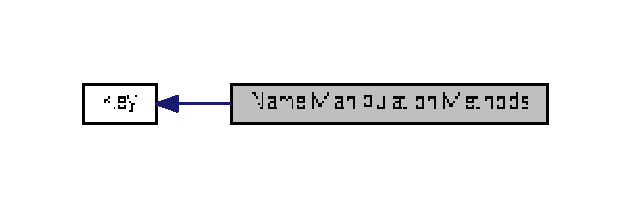
\includegraphics[width=290pt]{group__keyname}
\end{center}
\end{figure}
\subsection*{Enumerations}
\begin{DoxyCompactItemize}
\item 
enum \hyperlink{group__keyname_gaec3b8d6f430ae49b91bafe8a86310a68}{elektra\-Namespace} \{ \\*
\hyperlink{group__keyname_ggaec3b8d6f430ae49b91bafe8a86310a68a3659698b0a07454ca8055ab693e8efd1}{K\-E\-Y\-\_\-\-N\-S\-\_\-\-N\-O\-N\-E} =0, 
\hyperlink{group__keyname_ggaec3b8d6f430ae49b91bafe8a86310a68a33d6c53529b4e6921d0b1d6565df2f1f}{K\-E\-Y\-\_\-\-N\-S\-\_\-\-E\-M\-P\-T\-Y} =1, 
\hyperlink{group__keyname_ggaec3b8d6f430ae49b91bafe8a86310a68ac5fbf2c3a7ae79fa2d60c48ae3e72688}{K\-E\-Y\-\_\-\-N\-S\-\_\-\-M\-E\-T\-A} =1$<$$<$1, 
\hyperlink{group__keyname_ggaec3b8d6f430ae49b91bafe8a86310a68a2c9133e3095dccbcde5ca3bb13987b5d}{K\-E\-Y\-\_\-\-N\-S\-\_\-\-C\-A\-S\-C\-A\-D\-I\-N\-G} =1$<$$<$2, 
\\*
\hyperlink{group__keyname_ggaec3b8d6f430ae49b91bafe8a86310a68a8ce23c70010e8ac8bb540b0947e03a4e}{K\-E\-Y\-\_\-\-N\-S\-\_\-\-U\-S\-E\-R} =1$<$$<$3, 
\hyperlink{group__keyname_ggaec3b8d6f430ae49b91bafe8a86310a68a61adca2f9dff47e65dfcdb492ffa7a20}{K\-E\-Y\-\_\-\-N\-S\-\_\-\-S\-Y\-S\-T\-E\-M} =1$<$$<$4
 \}
\end{DoxyCompactItemize}
\subsection*{Functions}
\begin{DoxyCompactItemize}
\item 
const char $\ast$ \hyperlink{group__keyname_ga8e805c726a60da921d3736cda7813513}{key\-Name} (const Key $\ast$key)
\item 
ssize\-\_\-t \hyperlink{group__keyname_gabdbcfa51ed8a387e47ead207affa2d2e}{key\-Get\-Name\-Size} (const Key $\ast$key)
\item 
ssize\-\_\-t \hyperlink{group__keyname_gab29a850168d9b31c9529e90cf9ab68be}{key\-Get\-Name} (const Key $\ast$key, char $\ast$returned\-Name, size\-\_\-t max\-Size)
\item 
ssize\-\_\-t \hyperlink{group__keyname_ga7699091610e7f3f43d2949514a4b35d9}{key\-Set\-Name} (Key $\ast$key, const char $\ast$new\-Name)
\item 
ssize\-\_\-t \hyperlink{group__keyname_gab65dc9d43d3ee08d5e936a20ebbddd23}{key\-Get\-Full\-Name\-Size} (const Key $\ast$key)
\item 
ssize\-\_\-t \hyperlink{group__keyname_gaaba1494a5ffc976e0e56c43f4334a23c}{key\-Get\-Full\-Name} (const Key $\ast$key, char $\ast$returned\-Name, size\-\_\-t max\-Size)
\item 
\hyperlink{group__keyname_gaec3b8d6f430ae49b91bafe8a86310a68}{elektra\-Namespace} \hyperlink{group__keyname_gafc3ca03ed10f87eb59bdc02cf2a0de8d}{key\-Get\-Namespace} (const Key $\ast$key)
\item 
const char $\ast$ \hyperlink{group__keyname_gaaff35e7ca8af5560c47e662ceb9465f5}{key\-Base\-Name} (const Key $\ast$key)
\begin{DoxyCompactList}\small\item\em Returns a pointer to the internal unescaped key name where the {\ttfamily basename} starts. \end{DoxyCompactList}\item 
ssize\-\_\-t \hyperlink{group__keyname_ga1a0b76c5d9e5367c7e72211e6c63d43a}{key\-Get\-Base\-Name\-Size} (const Key $\ast$key)
\item 
ssize\-\_\-t \hyperlink{group__keyname_ga0992d26bcfca767cb8e77053a483eb64}{key\-Get\-Base\-Name} (const Key $\ast$key, char $\ast$returned, size\-\_\-t max\-Size)
\item 
ssize\-\_\-t \hyperlink{group__keyname_gaa942091fc4bd5c2699e49ddc50829524}{key\-Add\-Base\-Name} (Key $\ast$key, const char $\ast$base\-Name)
\item 
ssize\-\_\-t \hyperlink{group__keyname_ga6e804bd453f98c28b0ff51430d1df407}{key\-Set\-Base\-Name} (Key $\ast$key, const char $\ast$base\-Name)
\item 
const char $\ast$ \hyperlink{group__keyname_gaf6485fb8599714b6bbd830cf915ffea5}{key\-Owner} (const Key $\ast$key)
\item 
ssize\-\_\-t \hyperlink{group__keyname_ga4a4561895741ba2ad10acf007c188593}{key\-Get\-Owner\-Size} (const Key $\ast$key)
\item 
ssize\-\_\-t \hyperlink{group__keyname_ga35922a017bee8b4bcb493bbdfad9d6f5}{key\-Get\-Owner} (const Key $\ast$key, char $\ast$returned\-Owner, size\-\_\-t max\-Size)
\item 
ssize\-\_\-t \hyperlink{group__keyname_ga88d6ec200ba0707b7c1b4a88133d2be4}{key\-Set\-Owner} (Key $\ast$key, const char $\ast$new\-Owner)
\end{DoxyCompactItemize}


\subsection{Detailed Description}
Methods to do various operations on Key names. To use them\-: 
\begin{DoxyCode}
\textcolor{preprocessor}{#include <kdb.h>}
\end{DoxyCode}


These functions make it easier for C programmers to work with key names.

\begin{DoxyParagraph}{Terminology of Key Names}

\begin{DoxyItemize}
\item A {\itshape key name} (see \hyperlink{group__keyname_ga7699091610e7f3f43d2949514a4b35d9}{key\-Set\-Name()} and \hyperlink{group__keyname_ga8e805c726a60da921d3736cda7813513}{key\-Name()}) defines the place of a key within the key database. To be unique, it is always absolute and canonical.
\item Key names are composed out of many {\itshape key name parts} split by a separator. These {\itshape key name parts} do not contain a unescaped separator.
\item A {\itshape key base name} (see \hyperlink{group__keyname_ga6e804bd453f98c28b0ff51430d1df407}{key\-Set\-Base\-Name()} and \hyperlink{group__keyname_gaa942091fc4bd5c2699e49ddc50829524}{key\-Add\-Base\-Name()}) is the last part of the key name.
\item A namespace denotes the place the key comes from\-:
\begin{DoxyItemize}
\item {\itshape user} keys come from user's home directories
\item {\itshape system} keys come from systems etc directories
\end{DoxyItemize}
\item A {\itshape C-\/\-String} is a null terminated sequence of characters. So \textbackslash{}0 (null-\/character) must not occur within a C-\/\-String.
\end{DoxyItemize}
\end{DoxyParagraph}
\begin{DoxyNote}{Note}
The rules are currently not formally specified and are subject of change in the next major release. So, always prefer\-:
\begin{DoxyItemize}
\item To use \hyperlink{group__keyname_ga7699091610e7f3f43d2949514a4b35d9}{key\-Set\-Name()} and key\-Add\-Name() to get the canonified version of the keyname
\item To use \hyperlink{group__keyname_ga6e804bd453f98c28b0ff51430d1df407}{key\-Set\-Base\-Name()} and \hyperlink{group__keyname_gaa942091fc4bd5c2699e49ddc50829524}{key\-Add\-Base\-Name()} to get an escaped key name part.
\item Not to escape or canonify with your own algorithms!
\item To use key\-Unescaped\-Name() and \hyperlink{group__keyname_gaaff35e7ca8af5560c47e662ceb9465f5}{key\-Base\-Name()} to have access to the key name without escape sequences (key name parts are null terminated)
\item Not to unescape the strings yourself!
\end{DoxyItemize}
\end{DoxyNote}
\begin{DoxyParagraph}{Syntax for Key Names}
Key names and key name parts have following goals\-:
\begin{DoxyItemize}
\item The C-\/\-String passed to \hyperlink{group__keyname_ga7699091610e7f3f43d2949514a4b35d9}{key\-Set\-Name()} and key\-Add\-Name() may be any C-\/\-String.
\item The {\itshape key name parts} (e.\-g. \hyperlink{group__keyname_ga6e804bd453f98c28b0ff51430d1df407}{key\-Set\-Base\-Name()}, \hyperlink{group__keyname_gaaff35e7ca8af5560c47e662ceb9465f5}{key\-Base\-Name()}) may be any C-\/\-String. Escaping is needed to achieve both goals.
\end{DoxyItemize}
\end{DoxyParagraph}
\begin{DoxyParagraph}{Semantics for Key Name Parts}

\begin{DoxyItemize}
\item \% denotes an empty key name part.
\end{DoxyItemize}
\end{DoxyParagraph}
\begin{DoxyParagraph}{Canonicalization for Key Names}

\begin{DoxyItemize}
\item / (slash) is the separator between key name parts.
\item // is shortened to /
\item trailing / (slashes) are removed
\item . (dot) and .. (dot-\/dot) is removed in an canonical key name, with following rules\-:
\begin{DoxyItemize}
\item /./ is shortened to /
\item \-\_\-/../ is shortened to \-\_\-
\end{DoxyItemize}
\end{DoxyItemize}
\end{DoxyParagraph}
\begin{DoxyParagraph}{Conventions for key names}

\begin{DoxyItemize}
\item Key name parts starting with \# are array elements. Then only \-\_\- (underscore) followed by 0-\/9 is allowed. So we have the regular expression \#\mbox{[}\-\_\-\mbox{]}$\ast$\mbox{[}0-\/9\mbox{]}+ with the further limitation that the number of \-\_\- is defined by the number of digits-\/1.
\item Key name parts starting with \-\_\- are reserved for special purposes (if you use this within a plugin you still have to make sure \-\_\- is escaped properly)
\item Key name parts starting with @ are reserved for special purposes (if you use this within a plugin you still have to make sure @ is escaped properly)
\item If any key name part starts with . (dot) it means the key is inactive, see \hyperlink{group__keytest_gaa25f699f592031c1a0abc1504d14e13e}{key\-Is\-Inactive()}.
\end{DoxyItemize}
\end{DoxyParagraph}
\begin{DoxyParagraph}{Escaping rules}

\begin{DoxyItemize}
\item \textbackslash{} (backslash) is the escape character for the situations as described here (and only these). The \textbackslash{} character must only be escaped, when one of the following rules apply. So there is no stray escape character possible.
\item \textbackslash{}/ allows to escape /
\item \textbackslash{}\textbackslash{}/ allows to use \textbackslash{} as character before / (and so on)
\item Use  and . if you want your key name part to represent . and ..
\item \textbackslash{} and \textbackslash{}. allows to use \textbackslash{} as character before . and .. (and so on)
\item Use \textbackslash{}\% if you want your key name part to start with \% (and does not represent an empty name)
\item Use \textbackslash{}\textbackslash{}\% allows to use \textbackslash{} as character before \% (and so on)
\end{DoxyItemize}
\end{DoxyParagraph}
\begin{DoxyParagraph}{Semantics for Key Name Specifications}

\begin{DoxyItemize}
\item \-\_\- denotes that the key name part is arbitrary (syntax as described above).
\item \# denotes that the key name part has array syntax.
\item names surrounded by \% (e.\-g. \%profile\%) denotes a placeholder.
\end{DoxyItemize}
\end{DoxyParagraph}
\begin{DoxyParagraph}{Usage of Key Names}
When using Elektra to store your application's configuration and state, please keep in mind the following rules\-:
\begin{DoxyItemize}
\item Avoid to have your applications root right under {\ttfamily system} or {\ttfamily user}. (rationale\-: it would make the hierarchy too flat.)
\item Avoid the usage of characters other then a-\/z, 0-\/9 and \-\_\-. (rationale\-: it would allow too many similar, confusing names.) (exceptions\-: if the user or a technology, decide about parts of the key name, this restriction does not apply, e.\-g. if the wlan essid is used as part of the key name)
\item It is suggested to make your application look for default keys under {\ttfamily /sw/myapp/\#/\%/} where \# is a major version number, e.\-g. \#3 for the 4th version and \% is a profile (\% for default profile). This way, from a sysadmin perspective, it will be possible to copy the {\ttfamily system/sw/myapp/\#3/\%/} tree to something like {\ttfamily system/sw/myapp/\#3/old/} and keep system clean and organized. Additionally, it is possible to start the old version of the app, using {\ttfamily /sw/myapp/\#2}. 
\end{DoxyItemize}
\end{DoxyParagraph}


\subsection{Enumeration Type Documentation}
\hypertarget{group__keyname_gaec3b8d6f430ae49b91bafe8a86310a68}{\index{Name Manipulation Methods@{Name Manipulation Methods}!elektra\-Namespace@{elektra\-Namespace}}
\index{elektra\-Namespace@{elektra\-Namespace}!Name Manipulation Methods@{Name Manipulation Methods}}
\subsubsection[{elektra\-Namespace}]{\setlength{\rightskip}{0pt plus 5cm}enum {\bf elektra\-Namespace}}}\label{group__keyname_gaec3b8d6f430ae49b91bafe8a86310a68}
Elektra currently supported Key namespaces.

\begin{DoxySeeAlso}{See Also}
\hyperlink{group__kdb_ga28e385fd9cb7ccfe0b2f1ed2f62453a1}{kdb\-Get()}, \hyperlink{group__keyname_gafc3ca03ed10f87eb59bdc02cf2a0de8d}{key\-Get\-Namespace()} 
\end{DoxySeeAlso}
\begin{Desc}
\item[Enumerator\-: ]\par
\begin{description}
\index{K\-E\-Y\-\_\-\-N\-S\-\_\-\-N\-O\-N\-E@{K\-E\-Y\-\_\-\-N\-S\-\_\-\-N\-O\-N\-E}!Name Manipulation Methods@{Name Manipulation Methods}}\index{Name Manipulation Methods@{Name Manipulation Methods}!K\-E\-Y\-\_\-\-N\-S\-\_\-\-N\-O\-N\-E@{K\-E\-Y\-\_\-\-N\-S\-\_\-\-N\-O\-N\-E}}\item[{\em 
\hypertarget{group__keyname_ggaec3b8d6f430ae49b91bafe8a86310a68a3659698b0a07454ca8055ab693e8efd1}{K\-E\-Y\-\_\-\-N\-S\-\_\-\-N\-O\-N\-E}\label{group__keyname_ggaec3b8d6f430ae49b91bafe8a86310a68a3659698b0a07454ca8055ab693e8efd1}
}]no key given as parameter to \hyperlink{group__keyname_gafc3ca03ed10f87eb59bdc02cf2a0de8d}{key\-Get\-Namespace()} \index{K\-E\-Y\-\_\-\-N\-S\-\_\-\-E\-M\-P\-T\-Y@{K\-E\-Y\-\_\-\-N\-S\-\_\-\-E\-M\-P\-T\-Y}!Name Manipulation Methods@{Name Manipulation Methods}}\index{Name Manipulation Methods@{Name Manipulation Methods}!K\-E\-Y\-\_\-\-N\-S\-\_\-\-E\-M\-P\-T\-Y@{K\-E\-Y\-\_\-\-N\-S\-\_\-\-E\-M\-P\-T\-Y}}\item[{\em 
\hypertarget{group__keyname_ggaec3b8d6f430ae49b91bafe8a86310a68a33d6c53529b4e6921d0b1d6565df2f1f}{K\-E\-Y\-\_\-\-N\-S\-\_\-\-E\-M\-P\-T\-Y}\label{group__keyname_ggaec3b8d6f430ae49b91bafe8a86310a68a33d6c53529b4e6921d0b1d6565df2f1f}
}]key name was empty, e.\-g. invalid key name \index{K\-E\-Y\-\_\-\-N\-S\-\_\-\-M\-E\-T\-A@{K\-E\-Y\-\_\-\-N\-S\-\_\-\-M\-E\-T\-A}!Name Manipulation Methods@{Name Manipulation Methods}}\index{Name Manipulation Methods@{Name Manipulation Methods}!K\-E\-Y\-\_\-\-N\-S\-\_\-\-M\-E\-T\-A@{K\-E\-Y\-\_\-\-N\-S\-\_\-\-M\-E\-T\-A}}\item[{\em 
\hypertarget{group__keyname_ggaec3b8d6f430ae49b91bafe8a86310a68ac5fbf2c3a7ae79fa2d60c48ae3e72688}{K\-E\-Y\-\_\-\-N\-S\-\_\-\-M\-E\-T\-A}\label{group__keyname_ggaec3b8d6f430ae49b91bafe8a86310a68ac5fbf2c3a7ae79fa2d60c48ae3e72688}
}]meta key, i.\-e. any key name not under other categories \index{K\-E\-Y\-\_\-\-N\-S\-\_\-\-C\-A\-S\-C\-A\-D\-I\-N\-G@{K\-E\-Y\-\_\-\-N\-S\-\_\-\-C\-A\-S\-C\-A\-D\-I\-N\-G}!Name Manipulation Methods@{Name Manipulation Methods}}\index{Name Manipulation Methods@{Name Manipulation Methods}!K\-E\-Y\-\_\-\-N\-S\-\_\-\-C\-A\-S\-C\-A\-D\-I\-N\-G@{K\-E\-Y\-\_\-\-N\-S\-\_\-\-C\-A\-S\-C\-A\-D\-I\-N\-G}}\item[{\em 
\hypertarget{group__keyname_ggaec3b8d6f430ae49b91bafe8a86310a68a2c9133e3095dccbcde5ca3bb13987b5d}{K\-E\-Y\-\_\-\-N\-S\-\_\-\-C\-A\-S\-C\-A\-D\-I\-N\-G}\label{group__keyname_ggaec3b8d6f430ae49b91bafe8a86310a68a2c9133e3095dccbcde5ca3bb13987b5d}
}]cascading key, starts with /, abstract name for any of the namespaces below \index{K\-E\-Y\-\_\-\-N\-S\-\_\-\-U\-S\-E\-R@{K\-E\-Y\-\_\-\-N\-S\-\_\-\-U\-S\-E\-R}!Name Manipulation Methods@{Name Manipulation Methods}}\index{Name Manipulation Methods@{Name Manipulation Methods}!K\-E\-Y\-\_\-\-N\-S\-\_\-\-U\-S\-E\-R@{K\-E\-Y\-\_\-\-N\-S\-\_\-\-U\-S\-E\-R}}\item[{\em 
\hypertarget{group__keyname_ggaec3b8d6f430ae49b91bafe8a86310a68a8ce23c70010e8ac8bb540b0947e03a4e}{K\-E\-Y\-\_\-\-N\-S\-\_\-\-U\-S\-E\-R}\label{group__keyname_ggaec3b8d6f430ae49b91bafe8a86310a68a8ce23c70010e8ac8bb540b0947e03a4e}
}]user key in the home directory of the current user \index{K\-E\-Y\-\_\-\-N\-S\-\_\-\-S\-Y\-S\-T\-E\-M@{K\-E\-Y\-\_\-\-N\-S\-\_\-\-S\-Y\-S\-T\-E\-M}!Name Manipulation Methods@{Name Manipulation Methods}}\index{Name Manipulation Methods@{Name Manipulation Methods}!K\-E\-Y\-\_\-\-N\-S\-\_\-\-S\-Y\-S\-T\-E\-M@{K\-E\-Y\-\_\-\-N\-S\-\_\-\-S\-Y\-S\-T\-E\-M}}\item[{\em 
\hypertarget{group__keyname_ggaec3b8d6f430ae49b91bafe8a86310a68a61adca2f9dff47e65dfcdb492ffa7a20}{K\-E\-Y\-\_\-\-N\-S\-\_\-\-S\-Y\-S\-T\-E\-M}\label{group__keyname_ggaec3b8d6f430ae49b91bafe8a86310a68a61adca2f9dff47e65dfcdb492ffa7a20}
}]system key not in the home directory, shared for a computer system \end{description}
\end{Desc}



\subsection{Function Documentation}
\hypertarget{group__keyname_gaa942091fc4bd5c2699e49ddc50829524}{\index{Name Manipulation Methods@{Name Manipulation Methods}!key\-Add\-Base\-Name@{key\-Add\-Base\-Name}}
\index{key\-Add\-Base\-Name@{key\-Add\-Base\-Name}!Name Manipulation Methods@{Name Manipulation Methods}}
\subsubsection[{key\-Add\-Base\-Name}]{\setlength{\rightskip}{0pt plus 5cm}ssize\-\_\-t key\-Add\-Base\-Name (
\begin{DoxyParamCaption}
\item[{Key $\ast$}]{key, }
\item[{const char $\ast$}]{base\-Name}
\end{DoxyParamCaption}
)}}\label{group__keyname_gaa942091fc4bd5c2699e49ddc50829524}
Adds {\ttfamily base\-Name} (that will be escaped) to the current key name.

A new base\-Name will be added, no other part of the key name will be affected.

Assumes that {\ttfamily key} is a directory and will append {\ttfamily base\-Name} to it. The function adds the path separator for concatenating.

So if {\ttfamily key} has name {\ttfamily \char`\"{}system/dir1/dir2\char`\"{}} and this method is called with {\ttfamily base\-Name} {\ttfamily \char`\"{}mykey\char`\"{}}, the resulting key will have the name {\ttfamily \char`\"{}system/dir1/dir2/mykey\char`\"{}}.

When {\ttfamily base\-Name} is 0 nothing will happen and the size of the name is returned.

The escaping rules apply as in \hyperlink{group__keyname}{above }.

A simple example is\-: 
\begin{DoxyCodeInclude}
Key * k = \hyperlink{group__key_gad23c65b44bf48d773759e1f9a4d43b89}{keyNew}(\textcolor{stringliteral}{"user/my/long"}, \hyperlink{group__key_gga91fb3178848bd682000958089abbaf40aa8adb6fcb92dec58fb19410eacfdd403}{KEY\_END});
\hyperlink{group__keyname_gaa942091fc4bd5c2699e49ddc50829524}{keyAddBaseName}(k, \textcolor{stringliteral}{"myname"});
printf (\textcolor{stringliteral}{"%s\(\backslash\)n"}, \hyperlink{group__keyname_ga8e805c726a60da921d3736cda7813513}{keyName}(k)); \textcolor{comment}{// will print user/my/long/myname}
\hyperlink{group__key_ga3df95bbc2494e3e6703ece5639be5bb1}{keyDel}(k);
\end{DoxyCodeInclude}
 E.\-g. if you add . it will be escaped\-: 
\begin{DoxyCodeInclude}
\hyperlink{group__keyname_ga7699091610e7f3f43d2949514a4b35d9}{keySetName} (k, \textcolor{stringliteral}{"system/valid"});
succeed\_if (\hyperlink{group__keyname_gaa942091fc4bd5c2699e49ddc50829524}{keyAddBaseName} (k, \textcolor{stringliteral}{"."}) >= 0, \textcolor{stringliteral}{"could not add a base
       name"});
succeed\_if\_same\_string(\hyperlink{group__keyname_ga8e805c726a60da921d3736cda7813513}{keyName}(k), \textcolor{stringliteral}{"system/valid/\(\backslash\)\(\backslash\)."});
succeed\_if\_same\_string(\hyperlink{group__keyname_gaaff35e7ca8af5560c47e662ceb9465f5}{keyBaseName}(k), \textcolor{stringliteral}{"."});
\end{DoxyCodeInclude}
 \begin{DoxySeeAlso}{See Also}
\hyperlink{group__keyname_ga6e804bd453f98c28b0ff51430d1df407}{key\-Set\-Base\-Name()} to set a base name 

\hyperlink{group__keyname_ga7699091610e7f3f43d2949514a4b35d9}{key\-Set\-Name()} to set a new name.
\end{DoxySeeAlso}

\begin{DoxyParams}{Parameters}
{\em key} & the key object to work with \\
\hline
{\em base\-Name} & the string to append to the name \\
\hline
\end{DoxyParams}
\begin{DoxyReturn}{Returns}
the size in bytes of the new key name including the ending N\-U\-L\-L 

-\/1 if the key had no name 

-\/1 on N\-U\-L\-L pointers 
\end{DoxyReturn}

\begin{DoxyRetVals}{Return values}
{\em -\/1} & if key was inserted to a keyset before \\
\hline
\end{DoxyRetVals}
\hypertarget{group__keyname_gaaff35e7ca8af5560c47e662ceb9465f5}{\index{Name Manipulation Methods@{Name Manipulation Methods}!key\-Base\-Name@{key\-Base\-Name}}
\index{key\-Base\-Name@{key\-Base\-Name}!Name Manipulation Methods@{Name Manipulation Methods}}
\subsubsection[{key\-Base\-Name}]{\setlength{\rightskip}{0pt plus 5cm}const char$\ast$ key\-Base\-Name (
\begin{DoxyParamCaption}
\item[{const Key $\ast$}]{key}
\end{DoxyParamCaption}
)}}\label{group__keyname_gaaff35e7ca8af5560c47e662ceb9465f5}


Returns a pointer to the internal unescaped key name where the {\ttfamily basename} starts. 

This is a much more efficient version of \hyperlink{group__keyname_ga0992d26bcfca767cb8e77053a483eb64}{key\-Get\-Base\-Name()} and you should use it if you are responsible enough to not mess up things. The name might change or even point to a wrong place after a \hyperlink{group__keyname_ga7699091610e7f3f43d2949514a4b35d9}{key\-Set\-Name()}. So make sure to copy the memory before the name changes.

\hyperlink{group__keyname_gaaff35e7ca8af5560c47e662ceb9465f5}{key\-Base\-Name()} returns \char`\"{}\char`\"{} when there is no key\-Base\-Name. The reason is 
\begin{DoxyCodeInclude}
\hyperlink{group__keyname_ga7699091610e7f3f43d2949514a4b35d9}{keySetName}(k,\textcolor{stringliteral}{""});
succeed\_if\_same\_string(\hyperlink{group__keyname_gaaff35e7ca8af5560c47e662ceb9465f5}{keyBaseName}(k), \textcolor{stringliteral}{""});
\hyperlink{group__keyname_ga7699091610e7f3f43d2949514a4b35d9}{keySetName}(k,\textcolor{stringliteral}{"user"});
succeed\_if\_same\_string(\hyperlink{group__keyname_gaaff35e7ca8af5560c47e662ceb9465f5}{keyBaseName}(k), \textcolor{stringliteral}{""});
\end{DoxyCodeInclude}
 And there is also support for really empty basenames\-: 
\begin{DoxyCodeInclude}
\hyperlink{group__keyname_ga7699091610e7f3f43d2949514a4b35d9}{keySetName} (k, \textcolor{stringliteral}{"system/valid"});
succeed\_if (\hyperlink{group__keyname_gaa942091fc4bd5c2699e49ddc50829524}{keyAddBaseName} (k, \textcolor{stringliteral}{""}) >= 0, \textcolor{stringliteral}{"could not add a base
       name"});
succeed\_if\_same\_string(\hyperlink{group__keyname_ga8e805c726a60da921d3736cda7813513}{keyName}(k), \textcolor{stringliteral}{"system/valid/%"});
succeed\_if\_same\_string(\hyperlink{group__keyname_gaaff35e7ca8af5560c47e662ceb9465f5}{keyBaseName}(k), \textcolor{stringliteral}{""});
\end{DoxyCodeInclude}
 \begin{DoxyNote}{Note}
You must never use the pointer returned by \hyperlink{group__keyname_gaaff35e7ca8af5560c47e662ceb9465f5}{key\-Base\-Name()} method to change the name, but you should use \hyperlink{group__keyname_ga6e804bd453f98c28b0ff51430d1df407}{key\-Set\-Base\-Name()} instead.
\end{DoxyNote}

\begin{DoxyParams}{Parameters}
{\em key} & the object to obtain the basename from \\
\hline
\end{DoxyParams}
\begin{DoxyReturn}{Returns}
a pointer to the basename 

\char`\"{}\char`\"{} when the key has no (base)name 

0 on N\-U\-L\-L pointer 
\end{DoxyReturn}
\begin{DoxySeeAlso}{See Also}
\hyperlink{group__keyname_ga0992d26bcfca767cb8e77053a483eb64}{key\-Get\-Base\-Name()}, \hyperlink{group__keyname_ga1a0b76c5d9e5367c7e72211e6c63d43a}{key\-Get\-Base\-Name\-Size()} 

\hyperlink{group__keyname_ga8e805c726a60da921d3736cda7813513}{key\-Name()} to get a pointer to the name 

\hyperlink{group__keyname_gaf6485fb8599714b6bbd830cf915ffea5}{key\-Owner()} to get a pointer to the owner 
\end{DoxySeeAlso}
\hypertarget{group__keyname_ga0992d26bcfca767cb8e77053a483eb64}{\index{Name Manipulation Methods@{Name Manipulation Methods}!key\-Get\-Base\-Name@{key\-Get\-Base\-Name}}
\index{key\-Get\-Base\-Name@{key\-Get\-Base\-Name}!Name Manipulation Methods@{Name Manipulation Methods}}
\subsubsection[{key\-Get\-Base\-Name}]{\setlength{\rightskip}{0pt plus 5cm}ssize\-\_\-t key\-Get\-Base\-Name (
\begin{DoxyParamCaption}
\item[{const Key $\ast$}]{key, }
\item[{char $\ast$}]{returned, }
\item[{size\-\_\-t}]{max\-Size}
\end{DoxyParamCaption}
)}}\label{group__keyname_ga0992d26bcfca767cb8e77053a483eb64}
Calculate the basename of a key name and put it in {\ttfamily returned} finalizing the string with N\-U\-L\-L.

Some examples\-:
\begin{DoxyItemize}
\item basename of {\ttfamily system/some/keyname} is {\ttfamily keyname} 
\item basename of {\ttfamily \char`\"{}user/tmp/some key\char`\"{}} is {\ttfamily \char`\"{}some key\char`\"{}} 
\end{DoxyItemize}


\begin{DoxyParams}{Parameters}
{\em key} & the key to extract basename from \\
\hline
{\em returned} & a pre-\/allocated buffer to store the basename \\
\hline
{\em max\-Size} & size of the {\ttfamily returned} buffer \\
\hline
\end{DoxyParams}
\begin{DoxyReturn}{Returns}
number of bytes copied to {\ttfamily returned} 

1 on empty name 

-\/1 on N\-U\-L\-L pointers 

-\/1 when max\-Size is 0 or larger than S\-S\-I\-Z\-E\-\_\-\-M\-A\-X 
\end{DoxyReturn}
\begin{DoxySeeAlso}{See Also}
\hyperlink{group__keyname_gaaff35e7ca8af5560c47e662ceb9465f5}{key\-Base\-Name()}, \hyperlink{group__keyname_ga1a0b76c5d9e5367c7e72211e6c63d43a}{key\-Get\-Base\-Name\-Size()} 

\hyperlink{group__keyname_ga8e805c726a60da921d3736cda7813513}{key\-Name()}, \hyperlink{group__keyname_gab29a850168d9b31c9529e90cf9ab68be}{key\-Get\-Name()}, \hyperlink{group__keyname_ga7699091610e7f3f43d2949514a4b35d9}{key\-Set\-Name()} 
\end{DoxySeeAlso}
\hypertarget{group__keyname_ga1a0b76c5d9e5367c7e72211e6c63d43a}{\index{Name Manipulation Methods@{Name Manipulation Methods}!key\-Get\-Base\-Name\-Size@{key\-Get\-Base\-Name\-Size}}
\index{key\-Get\-Base\-Name\-Size@{key\-Get\-Base\-Name\-Size}!Name Manipulation Methods@{Name Manipulation Methods}}
\subsubsection[{key\-Get\-Base\-Name\-Size}]{\setlength{\rightskip}{0pt plus 5cm}ssize\-\_\-t key\-Get\-Base\-Name\-Size (
\begin{DoxyParamCaption}
\item[{const Key $\ast$}]{key}
\end{DoxyParamCaption}
)}}\label{group__keyname_ga1a0b76c5d9e5367c7e72211e6c63d43a}
Calculates number of bytes needed to store basename of {\ttfamily key}.

Key names that have only root names (e.\-g. {\ttfamily \char`\"{}system\char`\"{}} or {\ttfamily \char`\"{}user\char`\"{}} or {\ttfamily \char`\"{}user\-:domain\char`\"{}} ) does not have basenames, thus the function will return 1 bytes to store \char`\"{}\char`\"{}.

Basenames are denoted as\-:
\begin{DoxyItemize}
\item {\ttfamily system/some/thing/basename} -\/$>$ {\ttfamily basename} 
\item {\ttfamily user\-:domain/some/thing/base\textbackslash{}/name} $>$ {\ttfamily base\textbackslash{}/name} 
\end{DoxyItemize}


\begin{DoxyParams}{Parameters}
{\em key} & the key object to work with \\
\hline
\end{DoxyParams}
\begin{DoxyReturn}{Returns}
size in bytes of {\ttfamily key's} basename including ending N\-U\-L\-L 
\end{DoxyReturn}
\begin{DoxySeeAlso}{See Also}
\hyperlink{group__keyname_gaaff35e7ca8af5560c47e662ceb9465f5}{key\-Base\-Name()}, \hyperlink{group__keyname_ga0992d26bcfca767cb8e77053a483eb64}{key\-Get\-Base\-Name()} 

\hyperlink{group__keyname_ga8e805c726a60da921d3736cda7813513}{key\-Name()}, \hyperlink{group__keyname_gab29a850168d9b31c9529e90cf9ab68be}{key\-Get\-Name()}, \hyperlink{group__keyname_ga7699091610e7f3f43d2949514a4b35d9}{key\-Set\-Name()} 
\end{DoxySeeAlso}
\hypertarget{group__keyname_gaaba1494a5ffc976e0e56c43f4334a23c}{\index{Name Manipulation Methods@{Name Manipulation Methods}!key\-Get\-Full\-Name@{key\-Get\-Full\-Name}}
\index{key\-Get\-Full\-Name@{key\-Get\-Full\-Name}!Name Manipulation Methods@{Name Manipulation Methods}}
\subsubsection[{key\-Get\-Full\-Name}]{\setlength{\rightskip}{0pt plus 5cm}ssize\-\_\-t key\-Get\-Full\-Name (
\begin{DoxyParamCaption}
\item[{const Key $\ast$}]{key, }
\item[{char $\ast$}]{returned\-Name, }
\item[{size\-\_\-t}]{max\-Size}
\end{DoxyParamCaption}
)}}\label{group__keyname_gaaba1494a5ffc976e0e56c43f4334a23c}
Get key full name, including the user domain name.

\begin{DoxyReturn}{Returns}
number of bytes written 

1 on empty name 

-\/1 on N\-U\-L\-L pointers 

-\/1 if max\-Size is 0 or larger than S\-S\-I\-Z\-E\-\_\-\-M\-A\-X 
\end{DoxyReturn}

\begin{DoxyParams}{Parameters}
{\em key} & the key object \\
\hline
{\em returned\-Name} & pre-\/allocated memory to write the key name \\
\hline
{\em max\-Size} & maximum number of bytes that will fit in returned\-Name, including the final N\-U\-L\-L \\
\hline
\end{DoxyParams}
\hypertarget{group__keyname_gab65dc9d43d3ee08d5e936a20ebbddd23}{\index{Name Manipulation Methods@{Name Manipulation Methods}!key\-Get\-Full\-Name\-Size@{key\-Get\-Full\-Name\-Size}}
\index{key\-Get\-Full\-Name\-Size@{key\-Get\-Full\-Name\-Size}!Name Manipulation Methods@{Name Manipulation Methods}}
\subsubsection[{key\-Get\-Full\-Name\-Size}]{\setlength{\rightskip}{0pt plus 5cm}ssize\-\_\-t key\-Get\-Full\-Name\-Size (
\begin{DoxyParamCaption}
\item[{const Key $\ast$}]{key}
\end{DoxyParamCaption}
)}}\label{group__keyname_gab65dc9d43d3ee08d5e936a20ebbddd23}
Bytes needed to store the key name including user domain and ending N\-U\-L\-L.


\begin{DoxyParams}{Parameters}
{\em key} & the key object to work with \\
\hline
\end{DoxyParams}
\begin{DoxyReturn}{Returns}
number of bytes needed to store key name including user domain 

1 on empty name 

-\/1 on N\-U\-L\-L pointer 
\end{DoxyReturn}
\begin{DoxySeeAlso}{See Also}
\hyperlink{group__keyname_gaaba1494a5ffc976e0e56c43f4334a23c}{key\-Get\-Full\-Name()}, \hyperlink{group__keyname_gabdbcfa51ed8a387e47ead207affa2d2e}{key\-Get\-Name\-Size()} 
\end{DoxySeeAlso}
\hypertarget{group__keyname_gab29a850168d9b31c9529e90cf9ab68be}{\index{Name Manipulation Methods@{Name Manipulation Methods}!key\-Get\-Name@{key\-Get\-Name}}
\index{key\-Get\-Name@{key\-Get\-Name}!Name Manipulation Methods@{Name Manipulation Methods}}
\subsubsection[{key\-Get\-Name}]{\setlength{\rightskip}{0pt plus 5cm}ssize\-\_\-t key\-Get\-Name (
\begin{DoxyParamCaption}
\item[{const Key $\ast$}]{key, }
\item[{char $\ast$}]{returned\-Name, }
\item[{size\-\_\-t}]{max\-Size}
\end{DoxyParamCaption}
)}}\label{group__keyname_gab29a850168d9b31c9529e90cf9ab68be}
Get abbreviated key name (without owner name).

When there is not enough space to write the name, nothing will be written and -\/1 will be returned.

max\-Size is limited to S\-S\-I\-Z\-E\-\_\-\-M\-A\-X. When this value is exceeded -\/1 will be returned. The reason for that is that any value higher is just a negative return value passed by accident. Of course malloc is not as failure tolerant and will try to allocate.


\begin{DoxyCode}
\textcolor{keywordtype}{char} *getBack = malloc (\hyperlink{group__keyname_gabdbcfa51ed8a387e47ead207affa2d2e}{keyGetNameSize}(key));
\hyperlink{group__keyname_gab29a850168d9b31c9529e90cf9ab68be}{keyGetName}(key, getBack, \hyperlink{group__keyname_gabdbcfa51ed8a387e47ead207affa2d2e}{keyGetNameSize}(key));
\end{DoxyCode}


\begin{DoxyReturn}{Returns}
number of bytes written to {\ttfamily returned\-Name} 

1 when only a null was written 

-\/1 when keyname is longer then max\-Size or 0 or any N\-U\-L\-L pointer 
\end{DoxyReturn}

\begin{DoxyParams}{Parameters}
{\em key} & the key object to work with \\
\hline
{\em returned\-Name} & pre-\/allocated memory to write the key name \\
\hline
{\em max\-Size} & maximum number of bytes that will fit in returned\-Name, including the final N\-U\-L\-L \\
\hline
\end{DoxyParams}
\begin{DoxySeeAlso}{See Also}
\hyperlink{group__keyname_gabdbcfa51ed8a387e47ead207affa2d2e}{key\-Get\-Name\-Size()}, \hyperlink{group__keyname_gaaba1494a5ffc976e0e56c43f4334a23c}{key\-Get\-Full\-Name()}, \hyperlink{group__keyname_gab65dc9d43d3ee08d5e936a20ebbddd23}{key\-Get\-Full\-Name\-Size()} 
\end{DoxySeeAlso}
\hypertarget{group__keyname_gabdbcfa51ed8a387e47ead207affa2d2e}{\index{Name Manipulation Methods@{Name Manipulation Methods}!key\-Get\-Name\-Size@{key\-Get\-Name\-Size}}
\index{key\-Get\-Name\-Size@{key\-Get\-Name\-Size}!Name Manipulation Methods@{Name Manipulation Methods}}
\subsubsection[{key\-Get\-Name\-Size}]{\setlength{\rightskip}{0pt plus 5cm}ssize\-\_\-t key\-Get\-Name\-Size (
\begin{DoxyParamCaption}
\item[{const Key $\ast$}]{key}
\end{DoxyParamCaption}
)}}\label{group__keyname_gabdbcfa51ed8a387e47ead207affa2d2e}
Bytes needed to store the key name without owner.

For an empty key name you need one byte to store the ending N\-U\-L\-L. For that reason 1 is returned.


\begin{DoxyParams}{Parameters}
{\em key} & the key object to work with \\
\hline
\end{DoxyParams}
\begin{DoxyReturn}{Returns}
number of bytes needed, including ending N\-U\-L\-L, to store key name without owner 

1 if there is is no key Name 

-\/1 on N\-U\-L\-L pointer 
\end{DoxyReturn}
\begin{DoxySeeAlso}{See Also}
\hyperlink{group__keyname_gab29a850168d9b31c9529e90cf9ab68be}{key\-Get\-Name()}, \hyperlink{group__keyname_gab65dc9d43d3ee08d5e936a20ebbddd23}{key\-Get\-Full\-Name\-Size()} 
\end{DoxySeeAlso}
\hypertarget{group__keyname_gafc3ca03ed10f87eb59bdc02cf2a0de8d}{\index{Name Manipulation Methods@{Name Manipulation Methods}!key\-Get\-Namespace@{key\-Get\-Namespace}}
\index{key\-Get\-Namespace@{key\-Get\-Namespace}!Name Manipulation Methods@{Name Manipulation Methods}}
\subsubsection[{key\-Get\-Namespace}]{\setlength{\rightskip}{0pt plus 5cm}{\bf elektra\-Namespace} key\-Get\-Namespace (
\begin{DoxyParamCaption}
\item[{const Key $\ast$}]{key}
\end{DoxyParamCaption}
)}}\label{group__keyname_gafc3ca03ed10f87eb59bdc02cf2a0de8d}
For currently valid namespaces see \hyperlink{group__keyname_gaec3b8d6f430ae49b91bafe8a86310a68}{elektra\-Namespace}.

\begin{DoxyVersion}{Version}
0.\-8.\-10 Added method to kdbproposal.\-h
\end{DoxyVersion}
\begin{DoxyNote}{Note}
This method might be enhanced. You do not have any guarantee that, when for a specific name \hyperlink{group__keyname_ggaec3b8d6f430ae49b91bafe8a86310a68ac5fbf2c3a7ae79fa2d60c48ae3e72688}{K\-E\-Y\-\_\-\-N\-S\-\_\-\-M\-E\-T\-A} is returned today, that it still will be returned after the next recompilation. So make sure that your compiler gives you a warning for unhandled switches (gcc\-: -\/\-Wswitch or -\/\-Wswitch-\/enum if you want to handle default) and look out for those warnings.
\end{DoxyNote}

\begin{DoxyParams}{Parameters}
{\em key} & the key object to work with \\
\hline
\end{DoxyParams}
\begin{DoxyReturn}{Returns}
the namespace of a key. 
\end{DoxyReturn}
\hypertarget{group__keyname_ga35922a017bee8b4bcb493bbdfad9d6f5}{\index{Name Manipulation Methods@{Name Manipulation Methods}!key\-Get\-Owner@{key\-Get\-Owner}}
\index{key\-Get\-Owner@{key\-Get\-Owner}!Name Manipulation Methods@{Name Manipulation Methods}}
\subsubsection[{key\-Get\-Owner}]{\setlength{\rightskip}{0pt plus 5cm}ssize\-\_\-t key\-Get\-Owner (
\begin{DoxyParamCaption}
\item[{const Key $\ast$}]{key, }
\item[{char $\ast$}]{returned\-Owner, }
\item[{size\-\_\-t}]{max\-Size}
\end{DoxyParamCaption}
)}}\label{group__keyname_ga35922a017bee8b4bcb493bbdfad9d6f5}
Return the owner of the key.
\begin{DoxyItemize}
\item Given {\ttfamily user\-:someuser/}..... return {\ttfamily someuser} 
\item Given {\ttfamily user\-:some.\-user/}.... return {\ttfamily some.\-user} 
\item Given {\ttfamily user/}.... return the current user
\end{DoxyItemize}

Only {\ttfamily user/}... keys have a owner. For {\ttfamily system/}... keys (that doesn't have a key owner) an empty string (\char`\"{}\char`\"{}) is returned.

Although usually the same, the owner of a key is not related to its U\-I\-D. Owner are related to W\-H\-E\-R\-E the key is stored on disk, while U\-I\-Ds are related to mode controls of a key.


\begin{DoxyParams}{Parameters}
{\em key} & the object to work with \\
\hline
{\em returned\-Owner} & a pre-\/allocated space to store the owner \\
\hline
{\em max\-Size} & maximum number of bytes that fit returned \\
\hline
\end{DoxyParams}
\begin{DoxyReturn}{Returns}
number of bytes written to buffer 

1 if there is no owner 

-\/1 on N\-U\-L\-L pointers 

-\/1 when max\-Size is 0, larger than S\-S\-I\-Z\-E\-\_\-\-M\-A\-X or too small for ownername 
\end{DoxyReturn}
\begin{DoxySeeAlso}{See Also}
\hyperlink{group__keyname_ga7699091610e7f3f43d2949514a4b35d9}{key\-Set\-Name()}, \hyperlink{group__keyname_ga88d6ec200ba0707b7c1b4a88133d2be4}{key\-Set\-Owner()}, \hyperlink{group__keyname_gaf6485fb8599714b6bbd830cf915ffea5}{key\-Owner()}, \hyperlink{group__keyname_gaaba1494a5ffc976e0e56c43f4334a23c}{key\-Get\-Full\-Name()} 
\end{DoxySeeAlso}
\hypertarget{group__keyname_ga4a4561895741ba2ad10acf007c188593}{\index{Name Manipulation Methods@{Name Manipulation Methods}!key\-Get\-Owner\-Size@{key\-Get\-Owner\-Size}}
\index{key\-Get\-Owner\-Size@{key\-Get\-Owner\-Size}!Name Manipulation Methods@{Name Manipulation Methods}}
\subsubsection[{key\-Get\-Owner\-Size}]{\setlength{\rightskip}{0pt plus 5cm}ssize\-\_\-t key\-Get\-Owner\-Size (
\begin{DoxyParamCaption}
\item[{const Key $\ast$}]{key}
\end{DoxyParamCaption}
)}}\label{group__keyname_ga4a4561895741ba2ad10acf007c188593}
Return the size of the owner of the Key with concluding 0.

The returned number can be used to allocate a string. 1 will returned on an empty owner to store the concluding 0 on using \hyperlink{group__keyname_ga35922a017bee8b4bcb493bbdfad9d6f5}{key\-Get\-Owner()}.


\begin{DoxyCode}
\textcolor{keywordtype}{char} * buffer;
buffer = malloc (\hyperlink{group__keyname_ga4a4561895741ba2ad10acf007c188593}{keyGetOwnerSize} (key));
\textcolor{comment}{// use buffer and keyGetOwnerSize (key) for maxSize}
\end{DoxyCode}


\begin{DoxyNote}{Note}
that -\/1 might be returned on null pointer, so when you directly allocate afterwards its best to check if you will pass a null pointer before.
\end{DoxyNote}

\begin{DoxyParams}{Parameters}
{\em key} & the key object to work with \\
\hline
\end{DoxyParams}
\begin{DoxyReturn}{Returns}
number of bytes 

1 if there is no owner 

-\/1 on N\-U\-L\-L pointer 
\end{DoxyReturn}
\begin{DoxySeeAlso}{See Also}
\hyperlink{group__keyname_ga35922a017bee8b4bcb493bbdfad9d6f5}{key\-Get\-Owner()} 
\end{DoxySeeAlso}
\hypertarget{group__keyname_ga8e805c726a60da921d3736cda7813513}{\index{Name Manipulation Methods@{Name Manipulation Methods}!key\-Name@{key\-Name}}
\index{key\-Name@{key\-Name}!Name Manipulation Methods@{Name Manipulation Methods}}
\subsubsection[{key\-Name}]{\setlength{\rightskip}{0pt plus 5cm}const char$\ast$ key\-Name (
\begin{DoxyParamCaption}
\item[{const Key $\ast$}]{key}
\end{DoxyParamCaption}
)}}\label{group__keyname_ga8e805c726a60da921d3736cda7813513}
Returns a pointer to the abbreviated real internal {\ttfamily key} name.

This is a much more efficient version of \hyperlink{group__keyname_gab29a850168d9b31c9529e90cf9ab68be}{key\-Get\-Name()} and can use it if you are responsible enough to not mess up things. You are not allowed to change anything in the returned array. The content of that string may change after \hyperlink{group__keyname_ga7699091610e7f3f43d2949514a4b35d9}{key\-Set\-Name()} and similar functions. If you need a copy of the name, consider using \hyperlink{group__keyname_gab29a850168d9b31c9529e90cf9ab68be}{key\-Get\-Name()}.

The name will be without owner, see \hyperlink{group__keyname_gaaba1494a5ffc976e0e56c43f4334a23c}{key\-Get\-Full\-Name()} if you need the name with its owner.

\hyperlink{group__keyname_ga8e805c726a60da921d3736cda7813513}{key\-Name()} returns \char`\"{}\char`\"{} when there is no key\-Name. The reason is 
\begin{DoxyCode}
key=\hyperlink{group__key_gad23c65b44bf48d773759e1f9a4d43b89}{keyNew}(0);
\hyperlink{group__keyname_ga7699091610e7f3f43d2949514a4b35d9}{keySetName}(key,\textcolor{stringliteral}{""});
\hyperlink{group__keyname_ga8e805c726a60da921d3736cda7813513}{keyName}(key); \textcolor{comment}{// you would expect "" here}
\hyperlink{group__key_ga3df95bbc2494e3e6703ece5639be5bb1}{keyDel}(key);
\end{DoxyCode}


\begin{DoxyNote}{Note}
Note that the Key structure keeps its own size field that is calculated by library internal calls, so to avoid inconsistencies, you must never use the pointer returned by \hyperlink{group__keyname_ga8e805c726a60da921d3736cda7813513}{key\-Name()} method to set a new value. Use \hyperlink{group__keyname_ga7699091610e7f3f43d2949514a4b35d9}{key\-Set\-Name()} instead.
\end{DoxyNote}

\begin{DoxyParams}{Parameters}
{\em key} & the key object to work with \\
\hline
\end{DoxyParams}
\begin{DoxyReturn}{Returns}
a pointer to the keyname which must not be changed. 

\char`\"{}\char`\"{} when there is no (a empty) keyname 

0 on N\-U\-L\-L pointer 
\end{DoxyReturn}
\begin{DoxySeeAlso}{See Also}
\hyperlink{group__keyname_gabdbcfa51ed8a387e47ead207affa2d2e}{key\-Get\-Name\-Size()} for the string length 

\hyperlink{group__keyname_gaaba1494a5ffc976e0e56c43f4334a23c}{key\-Get\-Full\-Name()}, \hyperlink{group__keyname_gab65dc9d43d3ee08d5e936a20ebbddd23}{key\-Get\-Full\-Name\-Size()} to get the full name 

\hyperlink{group__keyname_gab29a850168d9b31c9529e90cf9ab68be}{key\-Get\-Name()} as alternative to get a copy 

\hyperlink{group__keyname_gaf6485fb8599714b6bbd830cf915ffea5}{key\-Owner()} to get a pointer to owner 
\end{DoxySeeAlso}
\hypertarget{group__keyname_gaf6485fb8599714b6bbd830cf915ffea5}{\index{Name Manipulation Methods@{Name Manipulation Methods}!key\-Owner@{key\-Owner}}
\index{key\-Owner@{key\-Owner}!Name Manipulation Methods@{Name Manipulation Methods}}
\subsubsection[{key\-Owner}]{\setlength{\rightskip}{0pt plus 5cm}const char$\ast$ key\-Owner (
\begin{DoxyParamCaption}
\item[{const Key $\ast$}]{key}
\end{DoxyParamCaption}
)}}\label{group__keyname_gaf6485fb8599714b6bbd830cf915ffea5}
Return a pointer to the real internal {\ttfamily key} owner.

This is a much more efficient version of \hyperlink{group__keyname_ga35922a017bee8b4bcb493bbdfad9d6f5}{key\-Get\-Owner()} and you should use it if you are responsible enough to not mess up things. You are not allowed to modify the returned string in any way. If you need a copy of the string, consider to use \hyperlink{group__keyname_ga35922a017bee8b4bcb493bbdfad9d6f5}{key\-Get\-Owner()} instead.

\hyperlink{group__keyname_gaf6485fb8599714b6bbd830cf915ffea5}{key\-Owner()} returns \char`\"{}\char`\"{} when there is no key\-Owner. The reason is 
\begin{DoxyCode}
key=\hyperlink{group__key_gad23c65b44bf48d773759e1f9a4d43b89}{keyNew}(0);
\hyperlink{group__keyname_ga88d6ec200ba0707b7c1b4a88133d2be4}{keySetOwner}(key,\textcolor{stringliteral}{""});
\hyperlink{group__keyname_gaf6485fb8599714b6bbd830cf915ffea5}{keyOwner}(key); \textcolor{comment}{// you would expect "" here}
\hyperlink{group__keyname_ga88d6ec200ba0707b7c1b4a88133d2be4}{keySetOwner}(key,\textcolor{stringliteral}{"system"});
\hyperlink{group__keyname_gaf6485fb8599714b6bbd830cf915ffea5}{keyOwner}(key); \textcolor{comment}{// you would expect "" here}
\end{DoxyCode}


\begin{DoxyNote}{Note}
Note that the Key structure keeps its own size field that is calculated by library internal calls, so to avoid inconsistencies, you must never use the pointer returned by \hyperlink{group__keyname_gaf6485fb8599714b6bbd830cf915ffea5}{key\-Owner()} method to set a new value. Use \hyperlink{group__keyname_ga88d6ec200ba0707b7c1b4a88133d2be4}{key\-Set\-Owner()} instead.
\end{DoxyNote}

\begin{DoxyParams}{Parameters}
{\em key} & the key object to work with \\
\hline
\end{DoxyParams}
\begin{DoxyReturn}{Returns}
a pointer to internal owner 
\end{DoxyReturn}

\begin{DoxyRetVals}{Return values}
{\em \char`\"{}\char`\"{}} & when there is no (a empty) owner \\
\hline
{\em 0} & iff key is a N\-U\-L\-L pointer \\
\hline
\end{DoxyRetVals}
\begin{DoxySeeAlso}{See Also}
\hyperlink{group__keyname_ga4a4561895741ba2ad10acf007c188593}{key\-Get\-Owner\-Size()} for the size of the string with concluding 0 

\hyperlink{group__keyname_ga35922a017bee8b4bcb493bbdfad9d6f5}{key\-Get\-Owner()}, \hyperlink{group__keyname_ga88d6ec200ba0707b7c1b4a88133d2be4}{key\-Set\-Owner()} 

\hyperlink{group__keyname_ga8e805c726a60da921d3736cda7813513}{key\-Name()} for name without owner 

\hyperlink{group__keyname_gaaba1494a5ffc976e0e56c43f4334a23c}{key\-Get\-Full\-Name()} for name with owner 
\end{DoxySeeAlso}
\hypertarget{group__keyname_ga6e804bd453f98c28b0ff51430d1df407}{\index{Name Manipulation Methods@{Name Manipulation Methods}!key\-Set\-Base\-Name@{key\-Set\-Base\-Name}}
\index{key\-Set\-Base\-Name@{key\-Set\-Base\-Name}!Name Manipulation Methods@{Name Manipulation Methods}}
\subsubsection[{key\-Set\-Base\-Name}]{\setlength{\rightskip}{0pt plus 5cm}ssize\-\_\-t key\-Set\-Base\-Name (
\begin{DoxyParamCaption}
\item[{Key $\ast$}]{key, }
\item[{const char $\ast$}]{base\-Name}
\end{DoxyParamCaption}
)}}\label{group__keyname_ga6e804bd453f98c28b0ff51430d1df407}
Sets {\ttfamily base\-Name} as the new basename for {\ttfamily key}.

Only the base\-Name will be affected and no other part of the key.

All text after the last {\ttfamily '/'} in the {\ttfamily key} keyname is erased and {\ttfamily base\-Name} is appended.

So let us suppose {\ttfamily key} has name {\ttfamily \char`\"{}system/dir1/dir2/key1\char`\"{}}. If {\ttfamily base\-Name} is {\ttfamily \char`\"{}key2\char`\"{}}, the resulting key name will be {\ttfamily \char`\"{}system/dir1/dir2/key2\char`\"{}}. If {\ttfamily base\-Name} is empty or N\-U\-L\-L, the resulting key name will be {\ttfamily \char`\"{}system/dir1/dir2\char`\"{}}.

This function does proper escaping on the supplied name argument.

You can use all names to set as basename (e.\-g. . (dot), .. (dot-\/dot), \% and \char`\"{}\char`\"{} (empty)). They will be properly escaped.

A simple example is\-: 
\begin{DoxyCodeInclude}
Key * k = \hyperlink{group__key_gad23c65b44bf48d773759e1f9a4d43b89}{keyNew}(\textcolor{stringliteral}{"user/my/long/name"}, \hyperlink{group__key_gga91fb3178848bd682000958089abbaf40aa8adb6fcb92dec58fb19410eacfdd403}{KEY\_END});
\hyperlink{group__keyname_ga6e804bd453f98c28b0ff51430d1df407}{keySetBaseName}(k, \textcolor{stringliteral}{"myname"});
printf (\textcolor{stringliteral}{"%s\(\backslash\)n"}, \hyperlink{group__keyname_ga8e805c726a60da921d3736cda7813513}{keyName}(k)); \textcolor{comment}{// will print user/my/long/myname}
\hyperlink{group__key_ga3df95bbc2494e3e6703ece5639be5bb1}{keyDel}(k);
\end{DoxyCodeInclude}
 If you do not want escaping, use \hyperlink{group__keyname_ga6e804bd453f98c28b0ff51430d1df407}{key\-Set\-Base\-Name()} instead. E.\-g. if you want to add an inactive key, use\-: 
\begin{DoxyCodeInclude}
        \hyperlink{group__keyname_ga7699091610e7f3f43d2949514a4b35d9}{keySetName} (k, \textcolor{stringliteral}{"system/valid"});
        \hyperlink{group__keyname_ga6e804bd453f98c28b0ff51430d1df407}{keySetBaseName}(k, \textcolor{stringliteral}{".hiddenkey"});
        succeed\_if\_same\_string(\hyperlink{group__keyname_ga8e805c726a60da921d3736cda7813513}{keyName}(k), \textcolor{stringliteral}{"system/.hiddenkey"});
        succeed\_if\_same\_string(\hyperlink{group__keyname_gaaff35e7ca8af5560c47e662ceb9465f5}{keyBaseName}(k), \textcolor{stringliteral}{".hiddenkey"});
\end{DoxyCodeInclude}
 or when you want to add an array item, use\-: 
\begin{DoxyCodeInclude}
        \hyperlink{group__keyname_ga7699091610e7f3f43d2949514a4b35d9}{keySetName} (k, \textcolor{stringliteral}{"system/valid"});
        \hyperlink{group__keyname_ga6e804bd453f98c28b0ff51430d1df407}{keySetBaseName}(k, \textcolor{stringliteral}{""});
        succeed\_if\_same\_string(\hyperlink{group__keyname_ga8e805c726a60da921d3736cda7813513}{keyName}(k), \textcolor{stringliteral}{"system/%"});
        succeed\_if\_same\_string(\hyperlink{group__keyname_gaaff35e7ca8af5560c47e662ceb9465f5}{keyBaseName}(k), \textcolor{stringliteral}{""});
\end{DoxyCodeInclude}
 \begin{DoxySeeAlso}{See Also}
\hyperlink{group__keyname}{Name Manipulation Methods} for more details on special names
\end{DoxySeeAlso}

\begin{DoxyParams}{Parameters}
{\em key} & the key object to work with \\
\hline
{\em base\-Name} & the string used to overwrite the basename of the key \\
\hline
\end{DoxyParams}
\begin{DoxyReturn}{Returns}
the size in bytes of the new key name 

-\/1 on N\-U\-L\-L pointers 
\end{DoxyReturn}

\begin{DoxyRetVals}{Return values}
{\em -\/1} & if key was inserted to a keyset before \\
\hline
\end{DoxyRetVals}
\begin{DoxySeeAlso}{See Also}
\hyperlink{group__keyname_gaa942091fc4bd5c2699e49ddc50829524}{key\-Add\-Base\-Name()} 

\hyperlink{group__keyname_ga7699091610e7f3f43d2949514a4b35d9}{key\-Set\-Name()} to set a new name 
\end{DoxySeeAlso}
\hypertarget{group__keyname_ga7699091610e7f3f43d2949514a4b35d9}{\index{Name Manipulation Methods@{Name Manipulation Methods}!key\-Set\-Name@{key\-Set\-Name}}
\index{key\-Set\-Name@{key\-Set\-Name}!Name Manipulation Methods@{Name Manipulation Methods}}
\subsubsection[{key\-Set\-Name}]{\setlength{\rightskip}{0pt plus 5cm}ssize\-\_\-t key\-Set\-Name (
\begin{DoxyParamCaption}
\item[{Key $\ast$}]{key, }
\item[{const char $\ast$}]{new\-Name}
\end{DoxyParamCaption}
)}}\label{group__keyname_ga7699091610e7f3f43d2949514a4b35d9}
Set a new name to a key.

A valid name is of the forms\-:
\begin{DoxyItemize}
\item {\ttfamily system/something} 
\item {\ttfamily user/something} 
\item {\ttfamily user\-:username/something} 
\end{DoxyItemize}

The last form has explicitly set the owner, to let the library know in which user folder to save the key. A owner is a user name. If it is not defined (the second form) current user is used.

You should always follow the guidelines for key tree structure creation.

A private copy of the key name will be stored, and the {\ttfamily new\-Name} parameter can be freed after this call.

.., . and / will be handled as in filesystem pathes. A valid name will be build out of the (valid) name what you pass, e.\-g. user///sw/../sw//././\-My\-App -\/$>$ user/sw/\-My\-App

On invalid names, N\-U\-L\-L or \char`\"{}\char`\"{} the name will be \char`\"{}\char`\"{} afterwards.


\begin{DoxyRetVals}{Return values}
{\em size} & in bytes of this new key name including ending N\-U\-L\-L \\
\hline
{\em 0} & if new\-Name is an empty string or a N\-U\-L\-L pointer (name will be empty afterwards) \\
\hline
{\em -\/1} & if new\-Name is invalid (name will be empty afterwards) \\
\hline
{\em -\/1} & if key was inserted to a keyset before \\
\hline
\end{DoxyRetVals}

\begin{DoxyParams}{Parameters}
{\em key} & the key object to work with \\
\hline
{\em new\-Name} & the new key name \\
\hline
\end{DoxyParams}
\begin{DoxySeeAlso}{See Also}
\hyperlink{group__key_gad23c65b44bf48d773759e1f9a4d43b89}{key\-New()}, \hyperlink{group__keyname_ga88d6ec200ba0707b7c1b4a88133d2be4}{key\-Set\-Owner()} 

\hyperlink{group__keyname_gab29a850168d9b31c9529e90cf9ab68be}{key\-Get\-Name()}, \hyperlink{group__keyname_gaaba1494a5ffc976e0e56c43f4334a23c}{key\-Get\-Full\-Name()}, \hyperlink{group__keyname_ga8e805c726a60da921d3736cda7813513}{key\-Name()} 

\hyperlink{group__keyname_ga6e804bd453f98c28b0ff51430d1df407}{key\-Set\-Base\-Name()}, \hyperlink{group__keyname_gaa942091fc4bd5c2699e49ddc50829524}{key\-Add\-Base\-Name()} to manipulate a name 
\end{DoxySeeAlso}
\hypertarget{group__keyname_ga88d6ec200ba0707b7c1b4a88133d2be4}{\index{Name Manipulation Methods@{Name Manipulation Methods}!key\-Set\-Owner@{key\-Set\-Owner}}
\index{key\-Set\-Owner@{key\-Set\-Owner}!Name Manipulation Methods@{Name Manipulation Methods}}
\subsubsection[{key\-Set\-Owner}]{\setlength{\rightskip}{0pt plus 5cm}ssize\-\_\-t key\-Set\-Owner (
\begin{DoxyParamCaption}
\item[{Key $\ast$}]{key, }
\item[{const char $\ast$}]{new\-Owner}
\end{DoxyParamCaption}
)}}\label{group__keyname_ga88d6ec200ba0707b7c1b4a88133d2be4}
Set the owner of a key.

A owner is a name of a system user related to a U\-I\-D. The owner decides on which location on the disc the key goes.

A private copy is stored, so the passed parameter can be freed after the call.


\begin{DoxyParams}{Parameters}
{\em key} & the key object to work with \\
\hline
{\em new\-Owner} & the string which describes the owner of the key \\
\hline
\end{DoxyParams}
\begin{DoxyReturn}{Returns}
the number of bytes actually saved including final N\-U\-L\-L 

1 when owner is freed (by setting 0 or \char`\"{}\char`\"{}) 

-\/1 on null pointer or memory problems 
\end{DoxyReturn}
\begin{DoxySeeAlso}{See Also}
\hyperlink{group__keyname_ga7699091610e7f3f43d2949514a4b35d9}{key\-Set\-Name()}, \hyperlink{group__keyname_ga35922a017bee8b4bcb493bbdfad9d6f5}{key\-Get\-Owner()}, \hyperlink{group__keyname_gaaba1494a5ffc976e0e56c43f4334a23c}{key\-Get\-Full\-Name()} 
\end{DoxySeeAlso}

\hypertarget{group__plugin}{\section{Plugins}
\label{group__plugin}\index{Plugins@{Plugins}}
}


Elektra plugin framework.  


\subsection*{Macros}
\begin{DoxyCompactItemize}
\item 
\#define \hyperlink{group__plugin_ga34d1a66f0a6e89cfd20f4014a9975a2a}{E\-L\-E\-K\-T\-R\-A\-\_\-\-P\-L\-U\-G\-I\-N\-\_\-\-F\-U\-N\-C\-T\-I\-O\-N}(module, function)~libelektra\-\_\-\#\#module\#\#\-\_\-\-L\-T\-X\-\_\-elektra\-Plugin\#\#function
\begin{DoxyCompactList}\small\item\em Declare a plugin's function name suitable for compilation variants (see doc/tutorials). \end{DoxyCompactList}\item 
\#define \hyperlink{group__plugin_ga78d616f68bf9fb0942f66478597467c6}{E\-L\-E\-K\-T\-R\-A\-\_\-\-R\-E\-A\-D\-M\-E}(module)~E\-L\-E\-K\-T\-R\-A\-\_\-\-R\-E\-A\-D\-M\-E2(module)
\begin{DoxyCompactList}\small\item\em The filename for inclusion of the readme for compilation variants (see doc/tutorials). \end{DoxyCompactList}\item 
\#define \hyperlink{group__plugin_gaab1842b82272e6d4235b6a71587a64d9}{E\-L\-E\-K\-T\-R\-A\-\_\-\-S\-E\-T\-\_\-\-E\-R\-R\-O\-R}(number, key, text)
\begin{DoxyCompactList}\small\item\em Sets the error in the keys metadata. \end{DoxyCompactList}\item 
\#define \hyperlink{group__plugin_ga3e4fc2c20d8e64bed7a54bb1af882e34}{E\-L\-E\-K\-T\-R\-A\-\_\-\-S\-E\-T\-\_\-\-E\-R\-R\-O\-R\-F}(number, key, formatstring,...)
\begin{DoxyCompactList}\small\item\em Sets the error in the keys metadata. \end{DoxyCompactList}\item 
\#define \hyperlink{group__plugin_ga2bbb3bc3a3bdaf5b34b52de81886a098}{E\-L\-E\-K\-T\-R\-A\-\_\-\-A\-D\-D\-\_\-\-W\-A\-R\-N\-I\-N\-G\-F}(number, key, formatstring,...)
\begin{DoxyCompactList}\small\item\em Adds an warning in the keys metadata. \end{DoxyCompactList}\item 
\#define \hyperlink{group__plugin_ga3da3bdb0f41710adda9eee3d7adac9ff}{E\-L\-E\-K\-T\-R\-A\-\_\-\-A\-D\-D\-\_\-\-W\-A\-R\-N\-I\-N\-G}(number, key, text)
\begin{DoxyCompactList}\small\item\em Adds an warning in the keys metadata. \end{DoxyCompactList}\end{DoxyCompactItemize}
\subsection*{Functions}
\begin{DoxyCompactItemize}
\item 
Plugin $\ast$ \hyperlink{group__plugin_ga8dd092048e972a3f0c9c9f54eb41576e}{elektra\-Plugin\-Export} (const char $\ast$plugin\-Name,...)
\begin{DoxyCompactList}\small\item\em Allows to Export Methods for a Plugin. \end{DoxyCompactList}\item 
Key\-Set $\ast$ \hyperlink{group__plugin_ga644bead796506c172817724051c977c9}{elektra\-Plugin\-Get\-Config} (Plugin $\ast$handle)
\begin{DoxyCompactList}\small\item\em Returns the configuration of that plugin. \end{DoxyCompactList}\item 
void \hyperlink{group__plugin_gaf4b941a52ff55d0ca2a9158d90208ef2}{elektra\-Plugin\-Set\-Data} (Plugin $\ast$plugin, void $\ast$data)
\begin{DoxyCompactList}\small\item\em Store a pointer to any plugin related data. \end{DoxyCompactList}\item 
void $\ast$ \hyperlink{group__plugin_gaafcf3216b46292f222b8cc7828b4dd20}{elektra\-Plugin\-Get\-Data} (Plugin $\ast$plugin)
\begin{DoxyCompactList}\small\item\em Get a pointer to any plugin related data stored before. \end{DoxyCompactList}\item 
int \hyperlink{group__plugin_ga23c2eb3584e38a4d494eb8f91e5e3d8d}{elektra\-Doc\-Open} (Plugin $\ast$handle, Key $\ast$warnings\-Key)
\begin{DoxyCompactList}\small\item\em Initialize data for the plugin. \end{DoxyCompactList}\item 
int \hyperlink{group__plugin_ga1236aefe5b2baf8b7bf636ba5aa9ea29}{elektra\-Doc\-Close} (Plugin $\ast$handle, Key $\ast$warnings\-Key)
\begin{DoxyCompactList}\small\item\em Finalize the plugin. \end{DoxyCompactList}\item 
int \hyperlink{group__plugin_gacb69f3441c6d84241b4362f958fbe313}{elektra\-Doc\-Get} (Plugin $\ast$handle, Key\-Set $\ast$returned, Key $\ast$parent\-Key)
\begin{DoxyCompactList}\small\item\em Get data from storage to application. \end{DoxyCompactList}\item 
int \hyperlink{group__plugin_gae65781a1deb34efc79c8cb9d9174842c}{elektra\-Doc\-Set} (Plugin $\ast$handle, Key\-Set $\ast$returned, Key $\ast$parent\-Key)
\begin{DoxyCompactList}\small\item\em Set data from application to storage. \end{DoxyCompactList}\item 
int \hyperlink{group__plugin_gad74b35f558ac7c3262f6069c5c47dc79}{elektra\-Doc\-Error} (Plugin $\ast$handle, Key\-Set $\ast$returned, Key $\ast$parent\-Key)
\begin{DoxyCompactList}\small\item\em Rollback in case of errors. \end{DoxyCompactList}\end{DoxyCompactItemize}


\subsection{Detailed Description}
Elektra plugin framework. \begin{DoxySince}{Since}
version 0.\-4.\-9, Elektra can dynamically load different key storage plugins.

version 0.\-7.\-0 Elektra can have multiple backends, mounted at any place in the key database.

version 0.\-8.\-0 Elektra backends are composed out of multiple plugins.
\end{DoxySince}
To get started with writing plugins, first read our plugin tutorial in doc/tutorials!

A plugin can implement any functionality related to configuration. There are 6 possible entry points for a plugin.
\begin{DoxyItemize}
\item \hyperlink{group__plugin_gacb69f3441c6d84241b4362f958fbe313}{elektra\-Doc\-Get()} will be called when configuration or the plugin's contract is retrieved from the key database
\item \hyperlink{group__plugin_gae65781a1deb34efc79c8cb9d9174842c}{elektra\-Doc\-Set()} will be called when configuration is written to the key database
\item \hyperlink{group__plugin_ga23c2eb3584e38a4d494eb8f91e5e3d8d}{elektra\-Doc\-Open()} will be called before any other method of the plugin is called
\item \hyperlink{group__plugin_ga1236aefe5b2baf8b7bf636ba5aa9ea29}{elektra\-Doc\-Close()} will be called as last method
\item \hyperlink{group__plugin_gad74b35f558ac7c3262f6069c5c47dc79}{elektra\-Doc\-Error()} will be called when \hyperlink{group__kdb_ga11436b058408f83d303ca5e996832bcf}{kdb\-Set()} failed (to give the plugin a chance to recover/undo its actions)
\item \hyperlink{group__plugin_ga8dd092048e972a3f0c9c9f54eb41576e}{elektra\-Plugin\-Export()} exports all methods for the plugin.
\end{DoxyItemize}

The names described here contain \char`\"{}\-Doc\char`\"{} within the method's name just because the plugin described in this document is called doc (the doxygen source was generated from src/plugins/doc/doc.\-h). Always replace Doc with the name of the plugin you are going to implement or use \hyperlink{group__plugin_ga34d1a66f0a6e89cfd20f4014a9975a2a}{E\-L\-E\-K\-T\-R\-A\-\_\-\-P\-L\-U\-G\-I\-N\-\_\-\-F\-U\-N\-C\-T\-I\-O\-N}.

\begin{DoxyParagraph}{Overview}
There are different types of plugins for different concerns. They all only have the entry points as defined above. The types of plugins handled in this document\-:
\begin{DoxyItemize}
\item A storage plugin gets an empty keyset in \hyperlink{group__plugin_gacb69f3441c6d84241b4362f958fbe313}{elektra\-Doc\-Get()} and constructs the information out from a file. In \hyperlink{group__plugin_gae65781a1deb34efc79c8cb9d9174842c}{elektra\-Doc\-Set()} the keyset is written to a file. \par
 Other persistent storage then a file is not handled within this document because it involves many other issues. For files the resolver plugin already takes care for transactions and rollback. So the storage plugin is the source and dump as known from pipes and filters.
\item A filter plugin is a plugin which operates on existing keys. It may process or change the keyset. Or it may reject specific keysets which do not meet some criteria.
\end{DoxyItemize}
\end{DoxyParagraph}
Use following include to have the functions that are not implement by you available\-:


\begin{DoxyCodeInclude}
\textcolor{preprocessor}{#include <kdbplugin.h>}
\end{DoxyCodeInclude}
 \begin{DoxyParagraph}{Error and Warnings}
In case of trouble, in some methods you can use the macro \hyperlink{group__plugin_gaab1842b82272e6d4235b6a71587a64d9}{E\-L\-E\-K\-T\-R\-A\-\_\-\-S\-E\-T\-\_\-\-E\-R\-R\-O\-R} (in other methods it is not allowed). You might add warnings with the macro \hyperlink{group__plugin_ga3da3bdb0f41710adda9eee3d7adac9ff}{E\-L\-E\-K\-T\-R\-A\-\_\-\-A\-D\-D\-\_\-\-W\-A\-R\-N\-I\-N\-G}. Read the documentation of the individual methods to decide what you should do.
\end{DoxyParagraph}
Use following include to have the macros for setting the error and adding the warnings available\-:


\begin{DoxyCodeInclude}
\textcolor{preprocessor}{#include <kdberrors.h>}
\end{DoxyCodeInclude}
 \begin{DoxySeeAlso}{See Also}
\href{http://www.libelektra.org/ftp/elektra/thesis.pdf}{\tt http\-://www.\-libelektra.\-org/ftp/elektra/thesis.\-pdf} for an detailed explanation and description of other types of plugins. Do not hesitate to ask at the mailinglist if anything is unclear. 
\end{DoxySeeAlso}


\subsection{Macro Definition Documentation}
\hypertarget{group__plugin_ga3da3bdb0f41710adda9eee3d7adac9ff}{\index{Plugins@{Plugins}!E\-L\-E\-K\-T\-R\-A\-\_\-\-A\-D\-D\-\_\-\-W\-A\-R\-N\-I\-N\-G@{E\-L\-E\-K\-T\-R\-A\-\_\-\-A\-D\-D\-\_\-\-W\-A\-R\-N\-I\-N\-G}}
\index{E\-L\-E\-K\-T\-R\-A\-\_\-\-A\-D\-D\-\_\-\-W\-A\-R\-N\-I\-N\-G@{E\-L\-E\-K\-T\-R\-A\-\_\-\-A\-D\-D\-\_\-\-W\-A\-R\-N\-I\-N\-G}!Plugins@{Plugins}}
\subsubsection[{E\-L\-E\-K\-T\-R\-A\-\_\-\-A\-D\-D\-\_\-\-W\-A\-R\-N\-I\-N\-G}]{\setlength{\rightskip}{0pt plus 5cm}\#define E\-L\-E\-K\-T\-R\-A\-\_\-\-A\-D\-D\-\_\-\-W\-A\-R\-N\-I\-N\-G(
\begin{DoxyParamCaption}
\item[{}]{number, }
\item[{}]{key, }
\item[{}]{text}
\end{DoxyParamCaption}
)}}\label{group__plugin_ga3da3bdb0f41710adda9eee3d7adac9ff}


Adds an warning in the keys metadata. 

Include kdberrors.\-h to make it work\-:


\begin{DoxyCodeInclude}
\textcolor{preprocessor}{#include <kdberrors.h>}
\end{DoxyCodeInclude}



\begin{DoxyParams}{Parameters}
{\em number} & the warning number from src/liberror/specification \\
\hline
{\em key} & to write the error to \\
\hline
{\em text} & additional text for the user \\
\hline
\end{DoxyParams}
\hypertarget{group__plugin_ga2bbb3bc3a3bdaf5b34b52de81886a098}{\index{Plugins@{Plugins}!E\-L\-E\-K\-T\-R\-A\-\_\-\-A\-D\-D\-\_\-\-W\-A\-R\-N\-I\-N\-G\-F@{E\-L\-E\-K\-T\-R\-A\-\_\-\-A\-D\-D\-\_\-\-W\-A\-R\-N\-I\-N\-G\-F}}
\index{E\-L\-E\-K\-T\-R\-A\-\_\-\-A\-D\-D\-\_\-\-W\-A\-R\-N\-I\-N\-G\-F@{E\-L\-E\-K\-T\-R\-A\-\_\-\-A\-D\-D\-\_\-\-W\-A\-R\-N\-I\-N\-G\-F}!Plugins@{Plugins}}
\subsubsection[{E\-L\-E\-K\-T\-R\-A\-\_\-\-A\-D\-D\-\_\-\-W\-A\-R\-N\-I\-N\-G\-F}]{\setlength{\rightskip}{0pt plus 5cm}\#define E\-L\-E\-K\-T\-R\-A\-\_\-\-A\-D\-D\-\_\-\-W\-A\-R\-N\-I\-N\-G\-F(
\begin{DoxyParamCaption}
\item[{}]{number, }
\item[{}]{key, }
\item[{}]{formatstring, }
\item[{}]{...}
\end{DoxyParamCaption}
)}}\label{group__plugin_ga2bbb3bc3a3bdaf5b34b52de81886a098}


Adds an warning in the keys metadata. 

Include kdberrors.\-h to make it work\-:


\begin{DoxyCodeInclude}
\textcolor{preprocessor}{#include <kdberrors.h>}
\end{DoxyCodeInclude}



\begin{DoxyParams}{Parameters}
{\em number} & the warning number from src/liberror/specification \\
\hline
{\em key} & to write the error to \\
\hline
{\em formatstring} & a format string as in printf \\
\hline
{\em ...} & further arguments as in printf \\
\hline
\end{DoxyParams}
\hypertarget{group__plugin_ga34d1a66f0a6e89cfd20f4014a9975a2a}{\index{Plugins@{Plugins}!E\-L\-E\-K\-T\-R\-A\-\_\-\-P\-L\-U\-G\-I\-N\-\_\-\-F\-U\-N\-C\-T\-I\-O\-N@{E\-L\-E\-K\-T\-R\-A\-\_\-\-P\-L\-U\-G\-I\-N\-\_\-\-F\-U\-N\-C\-T\-I\-O\-N}}
\index{E\-L\-E\-K\-T\-R\-A\-\_\-\-P\-L\-U\-G\-I\-N\-\_\-\-F\-U\-N\-C\-T\-I\-O\-N@{E\-L\-E\-K\-T\-R\-A\-\_\-\-P\-L\-U\-G\-I\-N\-\_\-\-F\-U\-N\-C\-T\-I\-O\-N}!Plugins@{Plugins}}
\subsubsection[{E\-L\-E\-K\-T\-R\-A\-\_\-\-P\-L\-U\-G\-I\-N\-\_\-\-F\-U\-N\-C\-T\-I\-O\-N}]{\setlength{\rightskip}{0pt plus 5cm}\#define E\-L\-E\-K\-T\-R\-A\-\_\-\-P\-L\-U\-G\-I\-N\-\_\-\-F\-U\-N\-C\-T\-I\-O\-N(
\begin{DoxyParamCaption}
\item[{}]{module, }
\item[{}]{function}
\end{DoxyParamCaption}
)~libelektra\-\_\-\#\#module\#\#\-\_\-\-L\-T\-X\-\_\-elektra\-Plugin\#\#function}}\label{group__plugin_ga34d1a66f0a6e89cfd20f4014a9975a2a}


Declare a plugin's function name suitable for compilation variants (see doc/tutorials). 

It can be used in the same way as \hyperlink{group__plugin_ga8dd092048e972a3f0c9c9f54eb41576e}{elektra\-Plugin\-Export()}. \begin{DoxySeeAlso}{See Also}
E\-L\-E\-K\-T\-R\-A\-\_\-\-P\-L\-U\-G\-I\-N\-\_\-\-E\-X\-P\-O\-R\-T
\end{DoxySeeAlso}

\begin{DoxyParams}{Parameters}
{\em plugin} & the name of the plugin \\
\hline
{\em which} & which function it is (open, close, get, set, error) \\
\hline
\end{DoxyParams}
\hypertarget{group__plugin_ga78d616f68bf9fb0942f66478597467c6}{\index{Plugins@{Plugins}!E\-L\-E\-K\-T\-R\-A\-\_\-\-R\-E\-A\-D\-M\-E@{E\-L\-E\-K\-T\-R\-A\-\_\-\-R\-E\-A\-D\-M\-E}}
\index{E\-L\-E\-K\-T\-R\-A\-\_\-\-R\-E\-A\-D\-M\-E@{E\-L\-E\-K\-T\-R\-A\-\_\-\-R\-E\-A\-D\-M\-E}!Plugins@{Plugins}}
\subsubsection[{E\-L\-E\-K\-T\-R\-A\-\_\-\-R\-E\-A\-D\-M\-E}]{\setlength{\rightskip}{0pt plus 5cm}\#define E\-L\-E\-K\-T\-R\-A\-\_\-\-R\-E\-A\-D\-M\-E(
\begin{DoxyParamCaption}
\item[{}]{module}
\end{DoxyParamCaption}
)~E\-L\-E\-K\-T\-R\-A\-\_\-\-R\-E\-A\-D\-M\-E2(module)}}\label{group__plugin_ga78d616f68bf9fb0942f66478597467c6}


The filename for inclusion of the readme for compilation variants (see doc/tutorials). 


\begin{DoxyParams}{Parameters}
{\em plugin} & the name of the plugin \\
\hline
\end{DoxyParams}
\hypertarget{group__plugin_gaab1842b82272e6d4235b6a71587a64d9}{\index{Plugins@{Plugins}!E\-L\-E\-K\-T\-R\-A\-\_\-\-S\-E\-T\-\_\-\-E\-R\-R\-O\-R@{E\-L\-E\-K\-T\-R\-A\-\_\-\-S\-E\-T\-\_\-\-E\-R\-R\-O\-R}}
\index{E\-L\-E\-K\-T\-R\-A\-\_\-\-S\-E\-T\-\_\-\-E\-R\-R\-O\-R@{E\-L\-E\-K\-T\-R\-A\-\_\-\-S\-E\-T\-\_\-\-E\-R\-R\-O\-R}!Plugins@{Plugins}}
\subsubsection[{E\-L\-E\-K\-T\-R\-A\-\_\-\-S\-E\-T\-\_\-\-E\-R\-R\-O\-R}]{\setlength{\rightskip}{0pt plus 5cm}\#define E\-L\-E\-K\-T\-R\-A\-\_\-\-S\-E\-T\-\_\-\-E\-R\-R\-O\-R(
\begin{DoxyParamCaption}
\item[{}]{number, }
\item[{}]{key, }
\item[{}]{text}
\end{DoxyParamCaption}
)}}\label{group__plugin_gaab1842b82272e6d4235b6a71587a64d9}


Sets the error in the keys metadata. 

Include kdberrors.\-h to make it work\-:


\begin{DoxyCodeInclude}
\textcolor{preprocessor}{#include <kdberrors.h>}
\end{DoxyCodeInclude}



\begin{DoxyParams}{Parameters}
{\em number} & the error number from src/liberror/specification \\
\hline
{\em key} & to write the error to \\
\hline
{\em text} & additional text for the user \\
\hline
\end{DoxyParams}
\hypertarget{group__plugin_ga3e4fc2c20d8e64bed7a54bb1af882e34}{\index{Plugins@{Plugins}!E\-L\-E\-K\-T\-R\-A\-\_\-\-S\-E\-T\-\_\-\-E\-R\-R\-O\-R\-F@{E\-L\-E\-K\-T\-R\-A\-\_\-\-S\-E\-T\-\_\-\-E\-R\-R\-O\-R\-F}}
\index{E\-L\-E\-K\-T\-R\-A\-\_\-\-S\-E\-T\-\_\-\-E\-R\-R\-O\-R\-F@{E\-L\-E\-K\-T\-R\-A\-\_\-\-S\-E\-T\-\_\-\-E\-R\-R\-O\-R\-F}!Plugins@{Plugins}}
\subsubsection[{E\-L\-E\-K\-T\-R\-A\-\_\-\-S\-E\-T\-\_\-\-E\-R\-R\-O\-R\-F}]{\setlength{\rightskip}{0pt plus 5cm}\#define E\-L\-E\-K\-T\-R\-A\-\_\-\-S\-E\-T\-\_\-\-E\-R\-R\-O\-R\-F(
\begin{DoxyParamCaption}
\item[{}]{number, }
\item[{}]{key, }
\item[{}]{formatstring, }
\item[{}]{...}
\end{DoxyParamCaption}
)}}\label{group__plugin_ga3e4fc2c20d8e64bed7a54bb1af882e34}


Sets the error in the keys metadata. 

Include kdberrors.\-h to make it work\-:


\begin{DoxyCodeInclude}
\textcolor{preprocessor}{#include <kdberrors.h>}
\end{DoxyCodeInclude}



\begin{DoxyParams}{Parameters}
{\em number} & the error number from src/liberror/specification \\
\hline
{\em key} & to write the error to \\
\hline
{\em formatstring} & a format string as in printf \\
\hline
{\em ...} & further arguments as in printf \\
\hline
\end{DoxyParams}


\subsection{Function Documentation}
\hypertarget{group__plugin_ga1236aefe5b2baf8b7bf636ba5aa9ea29}{\index{Plugins@{Plugins}!elektra\-Doc\-Close@{elektra\-Doc\-Close}}
\index{elektra\-Doc\-Close@{elektra\-Doc\-Close}!Plugins@{Plugins}}
\subsubsection[{elektra\-Doc\-Close}]{\setlength{\rightskip}{0pt plus 5cm}int elektra\-Doc\-Close (
\begin{DoxyParamCaption}
\item[{Plugin $\ast$}]{handle, }
\item[{Key $\ast$}]{warnings\-Key}
\end{DoxyParamCaption}
)}}\label{group__plugin_ga1236aefe5b2baf8b7bf636ba5aa9ea29}


Finalize the plugin. 

Called prior to unloading the plugin dynamic module. After this function is called, it is ensured that no functions from your plugin will ever be accessed again.

Make sure to free all memory that your plugin requested at runtime. Also make sure to free what you stored by \hyperlink{group__plugin_gaf4b941a52ff55d0ca2a9158d90208ef2}{elektra\-Plugin\-Set\-Data()} before.

So for the Doc plugin we need to\-:


\begin{DoxyCodeInclude}
\textcolor{keywordtype}{int} \hyperlink{group__plugin_ga1236aefe5b2baf8b7bf636ba5aa9ea29}{elektraDocClose}(Plugin *handle, Key *warningsKey 
      ELEKTRA\_UNUSED)
\{
        free (\hyperlink{group__plugin_gaafcf3216b46292f222b8cc7828b4dd20}{elektraPluginGetData}(handle));

        \textcolor{keywordflow}{return} 0; \textcolor{comment}{/* success */}
\}
\end{DoxyCodeInclude}
 After this call, libelektra.\-so will unload the plugin library, so this is the point to shutdown any affairs with the storage.


\begin{DoxyParams}{Parameters}
{\em handle} & contains internal information of the plugin \\
\hline
{\em warnings\-Key} & can be used to to add warnings using \hyperlink{group__plugin_ga3da3bdb0f41710adda9eee3d7adac9ff}{E\-L\-E\-K\-T\-R\-A\-\_\-\-A\-D\-D\-\_\-\-W\-A\-R\-N\-I\-N\-G} (Do not add errors!)\\
\hline
\end{DoxyParams}

\begin{DoxyRetVals}{Return values}
{\em 0} & on success (no other return value currently allowed)\\
\hline
{\em -\/1} & on problems (only use E\-L\-E\-K\-T\-R\-A\-\_\-\-A\-D\-D\-\_\-\-W\-A\-R\-N\-I\-N\-G, but never set an error).\\
\hline
\end{DoxyRetVals}
\begin{DoxySeeAlso}{See Also}
\hyperlink{group__kdb_gadb54dc9fda17ee07deb9444df745c96f}{kdb\-Close()} 

\hyperlink{group__plugin_gaafcf3216b46292f222b8cc7828b4dd20}{elektra\-Plugin\-Get\-Data()}, \hyperlink{group__plugin_gaf4b941a52ff55d0ca2a9158d90208ef2}{elektra\-Plugin\-Set\-Data()} and \hyperlink{group__plugin_ga644bead796506c172817724051c977c9}{elektra\-Plugin\-Get\-Config()} 
\end{DoxySeeAlso}
\hypertarget{group__plugin_gad74b35f558ac7c3262f6069c5c47dc79}{\index{Plugins@{Plugins}!elektra\-Doc\-Error@{elektra\-Doc\-Error}}
\index{elektra\-Doc\-Error@{elektra\-Doc\-Error}!Plugins@{Plugins}}
\subsubsection[{elektra\-Doc\-Error}]{\setlength{\rightskip}{0pt plus 5cm}int elektra\-Doc\-Error (
\begin{DoxyParamCaption}
\item[{Plugin $\ast$}]{handle, }
\item[{Key\-Set $\ast$}]{returned, }
\item[{Key $\ast$}]{parent\-Key}
\end{DoxyParamCaption}
)}}\label{group__plugin_gad74b35f558ac7c3262f6069c5c47dc79}


Rollback in case of errors. 

First for all plugins \hyperlink{group__plugin_gae65781a1deb34efc79c8cb9d9174842c}{elektra\-Doc\-Set()} will be called. If any plugin had problems before the commit (done by the resolver plugin), we can safely rollback our changes.

This method is rarely used by plugins, it is mainly used for resolvers (to implement rollback) or by logging plugins. It is not needed for storage plugins, because they only operate on temporary files created by the resolver.


\begin{DoxyParams}{Parameters}
{\em handle} & contains internal information of the plugin \\
\hline
{\em returned} & contains a keyset with relevant keys \\
\hline
{\em parent\-Key} & contains the information where to set the keys. can be used to add warnings with the macro \hyperlink{group__plugin_ga3da3bdb0f41710adda9eee3d7adac9ff}{E\-L\-E\-K\-T\-R\-A\-\_\-\-A\-D\-D\-\_\-\-W\-A\-R\-N\-I\-N\-G}, but do not add errors!\\
\hline
\end{DoxyParams}

\begin{DoxyRetVals}{Return values}
{\em 1} & on success \\
\hline
{\em 0} & on success with no action \\
\hline
{\em -\/1} & on failure (you can add warnings, but we are already in an error state, so do not set the error). \\
\hline
\end{DoxyRetVals}
\hypertarget{group__plugin_gacb69f3441c6d84241b4362f958fbe313}{\index{Plugins@{Plugins}!elektra\-Doc\-Get@{elektra\-Doc\-Get}}
\index{elektra\-Doc\-Get@{elektra\-Doc\-Get}!Plugins@{Plugins}}
\subsubsection[{elektra\-Doc\-Get}]{\setlength{\rightskip}{0pt plus 5cm}int elektra\-Doc\-Get (
\begin{DoxyParamCaption}
\item[{Plugin $\ast$}]{handle, }
\item[{Key\-Set $\ast$}]{returned, }
\item[{Key $\ast$}]{parent\-Key}
\end{DoxyParamCaption}
)}}\label{group__plugin_gacb69f3441c6d84241b4362f958fbe313}


Get data from storage to application. 

Retrieve information from a permanent storage to construct a keyset.\hypertarget{group__plugin_intro}{}\subsection{.}\label{group__plugin_intro}
The \hyperlink{group__plugin_gacb69f3441c6d84241b4362f958fbe313}{elektra\-Doc\-Get()} function handle everything related to receiving keys.\hypertarget{group__plugin_contract}{}\subsubsection{Contract Handling}\label{group__plugin_contract}
The contract is a keyset that needs to be returned if the parent\-Key is system/elektra/modules/yourpluginname.

Which keys and their meaning is specified in doc/\-C\-O\-N\-T\-R\-A\-C\-T.\-ini

Here is an example for our doc plugin\-:


\begin{DoxyCodeInclude}
\textcolor{keywordtype}{int} \hyperlink{group__plugin_gacb69f3441c6d84241b4362f958fbe313}{elektraDocGet}(Plugin *plugin ELEKTRA\_UNUSED, KeySet *returned,
       Key *parentKey)
\{
        \textcolor{keywordflow}{if} (!strcmp(\hyperlink{group__keyname_ga8e805c726a60da921d3736cda7813513}{keyName}(parentKey), \textcolor{stringliteral}{"system/elektra/modules/doc"}))
        \{
                KeySet *contract = \hyperlink{group__keyset_ga671e1aaee3ae9dc13b4834a4ddbd2c3c}{ksNew} (30,
                \hyperlink{group__key_gad23c65b44bf48d773759e1f9a4d43b89}{keyNew} (\textcolor{stringliteral}{"system/elektra/modules/doc"},
                        \hyperlink{group__key_gga91fb3178848bd682000958089abbaf40ac66e4a49d09212b79f5754ca6db5bd2e}{KEY\_VALUE}, \textcolor{stringliteral}{"doc plugin waits for your orders"},
       \hyperlink{group__key_gga91fb3178848bd682000958089abbaf40aa8adb6fcb92dec58fb19410eacfdd403}{KEY\_END}),
                \hyperlink{group__key_gad23c65b44bf48d773759e1f9a4d43b89}{keyNew} (\textcolor{stringliteral}{"system/elektra/modules/doc/exports"}, \hyperlink{group__key_gga91fb3178848bd682000958089abbaf40aa8adb6fcb92dec58fb19410eacfdd403}{KEY\_END}
      ),
                \hyperlink{group__key_gad23c65b44bf48d773759e1f9a4d43b89}{keyNew} (\textcolor{stringliteral}{"system/elektra/modules/doc/exports/open"},
                        KEY\_FUNC, \hyperlink{group__plugin_ga23c2eb3584e38a4d494eb8f91e5e3d8d}{elektraDocOpen}, \hyperlink{group__key_gga91fb3178848bd682000958089abbaf40aa8adb6fcb92dec58fb19410eacfdd403}{KEY\_END})
      ,
                \hyperlink{group__key_gad23c65b44bf48d773759e1f9a4d43b89}{keyNew} (\textcolor{stringliteral}{"system/elektra/modules/doc/exports/close"},
                        KEY\_FUNC, \hyperlink{group__plugin_ga1236aefe5b2baf8b7bf636ba5aa9ea29}{elektraDocClose}, \hyperlink{group__key_gga91fb3178848bd682000958089abbaf40aa8adb6fcb92dec58fb19410eacfdd403}{KEY\_END}
      ),
                \hyperlink{group__key_gad23c65b44bf48d773759e1f9a4d43b89}{keyNew} (\textcolor{stringliteral}{"system/elektra/modules/doc/exports/get"},
                        KEY\_FUNC, \hyperlink{group__plugin_gacb69f3441c6d84241b4362f958fbe313}{elektraDocGet}, \hyperlink{group__key_gga91fb3178848bd682000958089abbaf40aa8adb6fcb92dec58fb19410eacfdd403}{KEY\_END}),
                \hyperlink{group__key_gad23c65b44bf48d773759e1f9a4d43b89}{keyNew} (\textcolor{stringliteral}{"system/elektra/modules/doc/exports/set"},
                        KEY\_FUNC, \hyperlink{group__plugin_gae65781a1deb34efc79c8cb9d9174842c}{elektraDocSet}, \hyperlink{group__key_gga91fb3178848bd682000958089abbaf40aa8adb6fcb92dec58fb19410eacfdd403}{KEY\_END}),
                \hyperlink{group__key_gad23c65b44bf48d773759e1f9a4d43b89}{keyNew} (\textcolor{stringliteral}{"system/elektra/modules/doc/exports/error"},
                        KEY\_FUNC, \hyperlink{group__plugin_gad74b35f558ac7c3262f6069c5c47dc79}{elektraDocError}, \hyperlink{group__key_gga91fb3178848bd682000958089abbaf40aa8adb6fcb92dec58fb19410eacfdd403}{KEY\_END}
      ),
#include \hyperlink{group__plugin_ga78d616f68bf9fb0942f66478597467c6}{ELEKTRA\_README}(doc)
                \hyperlink{group__key_gad23c65b44bf48d773759e1f9a4d43b89}{keyNew} (\textcolor{stringliteral}{"system/elektra/modules/doc/infos/version"},
                        \hyperlink{group__key_gga91fb3178848bd682000958089abbaf40ac66e4a49d09212b79f5754ca6db5bd2e}{KEY\_VALUE}, PLUGINVERSION, \hyperlink{group__key_gga91fb3178848bd682000958089abbaf40aa8adb6fcb92dec58fb19410eacfdd403}{KEY\_END}),
                KS\_END);
                \hyperlink{group__keyset_ga21eb9c3a14a604ee3a8bdc779232e7b7}{ksAppend} (returned, contract);
                \hyperlink{group__keyset_ga27e5c16473b02a422238c8d970db7ac8}{ksDel} (contract);

                \textcolor{keywordflow}{return} 1; \textcolor{comment}{/* success */}
        \}
\end{DoxyCodeInclude}
 Some clauses of the contract, especially the description of the plugin can be done more conveniently directly in a R\-E\-A\-D\-M\-E.\-md that is included by \hyperlink{group__plugin_ga78d616f68bf9fb0942f66478597467c6}{E\-L\-E\-K\-T\-R\-A\-\_\-\-R\-E\-A\-D\-M\-E}.\hypertarget{group__plugin_storage}{}\subsubsection{Storage Plugins}\label{group__plugin_storage}
For storage plugins the filename is written in the value of the parent\-Key. So the first task of the plugin is to open that file. Then it should parse its content and construct a keyset with all information of that file.

You need to be able to reconstruct the same file with the information of the keyset. So be sure to copy all comments, whitespaces and so on into some metadata of the keys. Otherwise the information is lost after writing the file the next time.

Now lets look at an example how the typical \hyperlink{group__plugin_gacb69f3441c6d84241b4362f958fbe313}{elektra\-Doc\-Get()} might be implemented. To explain we introduce some pseudo functions which do all the work with the storage (which is of course 90\% of the work for a real plugin)\-:
\begin{DoxyItemize}
\item parse\-\_\-key will parse a key and a value from an open file handle
\end{DoxyItemize}

The typical loop for a storage plugin will be like\-:


\begin{DoxyCodeInclude}
        FILE *fp = fopen (\hyperlink{group__keyvalue_ga880936f2481d28e6e2acbe7486a21d05}{keyString}(parentKey), \textcolor{stringliteral}{"r"});
        \textcolor{keywordtype}{char} *key;
        \textcolor{keywordtype}{char} *value;

        \textcolor{keywordflow}{while} (parseKey(fp, &key, &value) >= 1)
        \{
                Key *read = \hyperlink{group__key_gad23c65b44bf48d773759e1f9a4d43b89}{keyNew}(0);
                \textcolor{keywordflow}{if} (\hyperlink{group__keyname_ga7699091610e7f3f43d2949514a4b35d9}{keySetName}(read, key) == -1)
                \{
                        fclose (fp);
                        \hyperlink{group__key_ga3df95bbc2494e3e6703ece5639be5bb1}{keyDel} (read);
                        \hyperlink{group__plugin_gaab1842b82272e6d4235b6a71587a64d9}{ELEKTRA\_SET\_ERROR}(59, parentKey, key);
                        \textcolor{keywordflow}{return} -1;
                \}
                \hyperlink{group__keyvalue_ga622bde1eb0e0c4994728331326340ef2}{keySetString}(read, value);

                \hyperlink{group__keyset_gaa5a1d467a4d71041edce68ea7748ce45}{ksAppendKey} (returned, read);
                free (key);
                free (value);
        \}

        \textcolor{keywordflow}{if} (feof(fp) == 0)
        \{
                fclose (fp);
                \hyperlink{group__plugin_gaab1842b82272e6d4235b6a71587a64d9}{ELEKTRA\_SET\_ERROR}(60, parentKey, \textcolor{stringliteral}{"not at the
       end of file"});
                \textcolor{keywordflow}{return} -1;
        \}

        fclose (fp);
\end{DoxyCodeInclude}
 \hypertarget{group__plugin_filter}{}\subsubsection{Filter Plugins}\label{group__plugin_filter}
For filter plugins the actual task is rather unspecified. You basically can do anything with the keyset. To get roundtrip properties you might want to undo any changes you did in \hyperlink{group__plugin_gae65781a1deb34efc79c8cb9d9174842c}{elektra\-Doc\-Set()}.

The pseudo functions (which do the real work) are\-:
\begin{DoxyItemize}
\item do\-\_\-action() which processes every key in this filter
\end{DoxyItemize}


\begin{DoxyCodeInclude}
        Key *k;
        \hyperlink{group__keyset_gabe793ff51f1728e3429c84a8a9086b70}{ksRewind} (returned);
        \textcolor{keywordflow}{while} ((k = \hyperlink{group__keyset_ga317321c9065b5a4b3e33fe1c399bcec9}{ksNext} (returned)) != 0)
        \{
                doAction(k);
        \}

        \textcolor{keywordflow}{return} 1; \textcolor{comment}{// success}
\}
\end{DoxyCodeInclude}
 \begin{DoxyPrecond}{Precondition}
The caller \hyperlink{group__kdb_ga28e385fd9cb7ccfe0b2f1ed2f62453a1}{kdb\-Get()} will make sure before you are called that the parent\-Key\-:
\begin{DoxyItemize}
\item is a valid key (means that it is a system or user key).
\item is your mountpoint and that your plugin is responsible for it. 
\end{DoxyItemize}

and that the returned\-:
\begin{DoxyItemize}
\item is a valid keyset.
\item your plugin is only called when needed (e.\-g. only if file was modified)
\item has {\ttfamily all} keys related to your plugin.
\item contains only valid keys below (see \hyperlink{group__keytest_ga03332b5d97c76a4fd2640aca4762b8df}{key\-Is\-Below()}) your parent\-Key.
\item is in a sorted order (given implicit by Key\-Set) 
\end{DoxyItemize}

and that the handle\-:
\begin{DoxyItemize}
\item is valid for your plugin.
\item that \hyperlink{group__plugin_gaafcf3216b46292f222b8cc7828b4dd20}{elektra\-Plugin\-Get\-Data()} contains the same handle for lifetime of your plugin.
\end{DoxyItemize}

The caller \hyperlink{group__kdb_ga28e385fd9cb7ccfe0b2f1ed2f62453a1}{kdb\-Get()} will make sure that afterwards you were called, that\-:
\begin{DoxyItemize}
\item other plugins below your plugin will be called again recursively.
\item that all keys are merged to one keyset the user gets
\item that all keys (that should not be removed) are passed to \hyperlink{group__kdb_ga11436b058408f83d303ca5e996832bcf}{kdb\-Set()} if writing to disc is needed.
\end{DoxyItemize}
\end{DoxyPrecond}
\begin{DoxyInvariant}{Invariant}
There are no global variables and \hyperlink{group__plugin_gaf4b941a52ff55d0ca2a9158d90208ef2}{elektra\-Plugin\-Set\-Data()} stores all information. The handle is to be guaranteed to be the same if it is the same plugin.
\end{DoxyInvariant}
\begin{DoxyPostcond}{Postcondition}
The keyset {\ttfamily returned} has the {\ttfamily parent\-Key} and all keys below (\hyperlink{group__keytest_ga03332b5d97c76a4fd2640aca4762b8df}{key\-Is\-Below()}) with all information from the storage. Make sure to return all keys, all directories and also all hidden keys. If some of them are not wished, the caller \hyperlink{group__kdb_ga28e385fd9cb7ccfe0b2f1ed2f62453a1}{kdb\-Get()} will drop these keys with additional plugins.
\end{DoxyPostcond}
\begin{DoxyParagraph}{Updating}
To get all keys out of the storage over and over again can be very inefficient. You might know a more efficient method to know if the key needs update or not, e.\-g. by stating it or by an external time stamp info. For file storage plugins this is automatically done for you by the resolver. For other types (e.\-g. databases) you need to implement your own resolver doing this.
\end{DoxyParagraph}
\begin{DoxySeeAlso}{See Also}
\hyperlink{group__kdb_ga28e385fd9cb7ccfe0b2f1ed2f62453a1}{kdb\-Get()} for caller.
\end{DoxySeeAlso}

\begin{DoxyParams}{Parameters}
{\em handle} & contains internal information of \hyperlink{group__kdb_ga6808defe5870f328dd17910aacbdc6ca}{opened } key database \\
\hline
{\em returned} & contains a keyset where the function need to append the keys got from the storage. There might be also some keys inside it, see conditions. You may use them to support efficient updating of keys, see updating. \\
\hline
{\em parent\-Key} & contains the information below which key the keys should be gotten.\\
\hline
\end{DoxyParams}
\begin{DoxyReturn}{Returns}
1 on success 

0 when nothing was to do 

-\/1 on failure, the current key in returned shows the position. use \hyperlink{group__plugin_gaab1842b82272e6d4235b6a71587a64d9}{E\-L\-E\-K\-T\-R\-A\-\_\-\-S\-E\-T\-\_\-\-E\-R\-R\-O\-R} of kdberrors.\-h to define the error code. You additionally can add as many warnings as you would like to add. 
\end{DoxyReturn}
\hypertarget{group__plugin_ga23c2eb3584e38a4d494eb8f91e5e3d8d}{\index{Plugins@{Plugins}!elektra\-Doc\-Open@{elektra\-Doc\-Open}}
\index{elektra\-Doc\-Open@{elektra\-Doc\-Open}!Plugins@{Plugins}}
\subsubsection[{elektra\-Doc\-Open}]{\setlength{\rightskip}{0pt plus 5cm}int elektra\-Doc\-Open (
\begin{DoxyParamCaption}
\item[{Plugin $\ast$}]{handle, }
\item[{Key $\ast$}]{warnings\-Key}
\end{DoxyParamCaption}
)}}\label{group__plugin_ga23c2eb3584e38a4d494eb8f91e5e3d8d}


Initialize data for the plugin. 

This is the first method called after dynamically loading this plugin. It is guaranteed, that this method will be called before any other method.

This method is responsible for\-:
\begin{DoxyItemize}
\item plugin's specific configuration gathering
\item initialization of all plugin's internal structs
\item initial setup of all I/\-O details such as opening a file, connecting to a database, setup connection to a server, iff this cannot be done per invocation in \hyperlink{group__plugin_gacb69f3441c6d84241b4362f958fbe313}{elektra\-Doc\-Get()} and \hyperlink{group__plugin_gae65781a1deb34efc79c8cb9d9174842c}{elektra\-Doc\-Set()}.
\end{DoxyItemize}

You may also read the configuration you can get with \hyperlink{group__plugin_ga644bead796506c172817724051c977c9}{elektra\-Plugin\-Get\-Config()} and transform it into other structures used by your plugin.

\begin{DoxyNote}{Note}
The plugin must not have any global variables. If you have one Elektra will not be threadsafe. Do not assume that your plugin will be opened only once or will not be reopened at a later time.
\end{DoxyNote}
Instead of global variables the methods \hyperlink{group__plugin_gaafcf3216b46292f222b8cc7828b4dd20}{elektra\-Plugin\-Get\-Data()} and \hyperlink{group__plugin_gaf4b941a52ff55d0ca2a9158d90208ef2}{elektra\-Plugin\-Set\-Data()} exist to store and get any information related to your plugin.

The correct substitute for global variables will be\-:


\begin{DoxyCodeInclude}
\textcolor{keyword}{typedef} \textcolor{keyword}{struct }\{ \textcolor{keywordtype}{int} global; \} GlobalData;
\end{DoxyCodeInclude}
 and then initialize it using\-:


\begin{DoxyCodeInclude}
\textcolor{keywordtype}{int} \hyperlink{group__plugin_ga23c2eb3584e38a4d494eb8f91e5e3d8d}{elektraDocOpen}(Plugin *handle, Key *warningsKey 
      ELEKTRA\_UNUSED)
\{
        GlobalData *data;
        KeySet *config = \hyperlink{group__plugin_ga644bead796506c172817724051c977c9}{elektraPluginGetConfig}(handle);
        Key * kg = \hyperlink{group__keyset_gad2e30fb6d4739d917c5abb2ac2f9c1a1}{ksLookupByName}(config, \textcolor{stringliteral}{"/global"}, 0);

        data=malloc(\textcolor{keyword}{sizeof}(GlobalData));
        data->global = 0;
        \textcolor{keywordflow}{if} (kg) data->global = atoi(\hyperlink{group__keyvalue_ga880936f2481d28e6e2acbe7486a21d05}{keyString}(kg));
        \hyperlink{group__plugin_gaf4b941a52ff55d0ca2a9158d90208ef2}{elektraPluginSetData}(handle,data);
\end{DoxyCodeInclude}
 Make sure to free everything you allocate within \hyperlink{group__plugin_ga1236aefe5b2baf8b7bf636ba5aa9ea29}{elektra\-Doc\-Close()}.

If your plugin has no useful way to startup without config, the module loader would not be able to load the module. To solve that problem the module loader adds the configuration key /module. Even if your plugin is basically not able to startup successfully, it should still provide a fallback when /module is present, so that \hyperlink{group__plugin_gacb69f3441c6d84241b4362f958fbe313}{elektra\-Doc\-Get()} on system/elektra/modules can be called successfully later on.


\begin{DoxyCodeInclude}
        \textcolor{keywordflow}{if} (\hyperlink{group__keyset_gad2e30fb6d4739d917c5abb2ac2f9c1a1}{ksLookupByName}(config, \textcolor{stringliteral}{"/module"}, 0))
        \{
                \textcolor{keywordflow}{return} 0;
        \}
        \textcolor{comment}{// do some setup that will fail without configuration}
\end{DoxyCodeInclude}
 
\begin{DoxyRetVals}{Return values}
{\em -\/1} & on error, your plugin will be removed then and the missing plugin added instead. Use \hyperlink{group__plugin_ga3da3bdb0f41710adda9eee3d7adac9ff}{E\-L\-E\-K\-T\-R\-A\-\_\-\-A\-D\-D\-\_\-\-W\-A\-R\-N\-I\-N\-G} to indicate the problem. The system will automatically add the information that the plugin was removed, so you do not need the user give that information.\\
\hline
{\em 0} & on success\\
\hline
\end{DoxyRetVals}

\begin{DoxyParams}{Parameters}
{\em handle} & contains internal information of the plugin \\
\hline
{\em warnings\-Key} & can be used to add warnings with the macro \hyperlink{group__plugin_ga3da3bdb0f41710adda9eee3d7adac9ff}{E\-L\-E\-K\-T\-R\-A\-\_\-\-A\-D\-D\-\_\-\-W\-A\-R\-N\-I\-N\-G} (Do not add errors!) \\
\hline
\end{DoxyParams}
\begin{DoxySeeAlso}{See Also}
\hyperlink{group__plugin_gaafcf3216b46292f222b8cc7828b4dd20}{elektra\-Plugin\-Get\-Data()}, \hyperlink{group__plugin_gaf4b941a52ff55d0ca2a9158d90208ef2}{elektra\-Plugin\-Set\-Data()} and \hyperlink{group__plugin_ga644bead796506c172817724051c977c9}{elektra\-Plugin\-Get\-Config()} 

\hyperlink{group__plugin_ga1236aefe5b2baf8b7bf636ba5aa9ea29}{elektra\-Doc\-Close()} 
\end{DoxySeeAlso}
\hypertarget{group__plugin_gae65781a1deb34efc79c8cb9d9174842c}{\index{Plugins@{Plugins}!elektra\-Doc\-Set@{elektra\-Doc\-Set}}
\index{elektra\-Doc\-Set@{elektra\-Doc\-Set}!Plugins@{Plugins}}
\subsubsection[{elektra\-Doc\-Set}]{\setlength{\rightskip}{0pt plus 5cm}int elektra\-Doc\-Set (
\begin{DoxyParamCaption}
\item[{Plugin $\ast$}]{handle, }
\item[{Key\-Set $\ast$}]{returned, }
\item[{Key $\ast$}]{parent\-Key}
\end{DoxyParamCaption}
)}}\label{group__plugin_gae65781a1deb34efc79c8cb9d9174842c}


Set data from application to storage. 

This function does everything related to set and remove keys in a plugin. There is only one function for that purpose to make implementation of file based plugins much easier.

The keyset {\ttfamily returned} was filled in with information from the application using elektra and the task of this function is to store it in a permanent way so that a subsequent call of elektra\-Plugin\-Get() can rebuild the keyset as it was before. See the live cycle to understand\-:


\begin{DoxyCodeInclude}
\textcolor{keyword}{static} \textcolor{keywordtype}{void} usercode (KDB *handle, KeySet *keyset, Key *key)
\{
        \textcolor{comment}{// some more user code}
        \hyperlink{group__keyvalue_ga622bde1eb0e0c4994728331326340ef2}{keySetString} (key, \textcolor{stringliteral}{"mycomment"}); \textcolor{comment}{// the user changes the
       key}
        \hyperlink{group__keyset_gaa5a1d467a4d71041edce68ea7748ce45}{ksAppendKey}(keyset, key); \textcolor{comment}{// append the key to the keyset}
        \hyperlink{group__kdb_ga11436b058408f83d303ca5e996832bcf}{kdbSet} (handle, keyset, 0); \textcolor{comment}{// and syncs it to disc}
\}

\textcolor{comment}{// so now kdbSet is called}
\textcolor{keywordtype}{int} elektraKdbSet(KDB *handle, KeySet *keyset, Key *parentKey)
\{
        \textcolor{keywordtype}{int} ret = 0;
        \textcolor{comment}{// find appropriate plugin and then call it:}
        Plugin *plugin = findPlugin(handle);
        ret = \hyperlink{group__plugin_gae65781a1deb34efc79c8cb9d9174842c}{elektraDocSet} (plugin, keyset, parentKey);
        \textcolor{comment}{// the keyset with the key (and others for this plugin)}
        \textcolor{comment}{// will be passed to this function}
        \textcolor{keywordflow}{return} ret;
\}

\textcolor{comment}{// so now elektraPluginSet(), which is the function described here,}
\textcolor{comment}{// is called:}
\textcolor{keywordtype}{int} elektraPluginSet(Plugin *plugin ELEKTRA\_UNUSED, KeySet *returned, Key *
      parentKey ELEKTRA\_UNUSED)
\{
        \textcolor{comment}{// the task of elektraPluginSet is now to store the keys}
        Key *k;
        \hyperlink{group__keyset_gabe793ff51f1728e3429c84a8a9086b70}{ksRewind} (returned);
        \textcolor{keywordflow}{while} ((k = \hyperlink{group__keyset_ga317321c9065b5a4b3e33fe1c399bcec9}{ksNext} (returned)) != 0)
        \{
                saveToDisc (k);
        \}

        \textcolor{keywordflow}{return} 1; \textcolor{comment}{/* success */}
\}
\end{DoxyCodeInclude}
 Of course all information of every key in the keyset {\ttfamily returned} need to be stored permanently. So this specification needs to give an exhaustive list of information present in a key.

\begin{DoxyPrecond}{Precondition}
The keyset {\ttfamily returned} holds all keys which must be saved permanently for this keyset. The keyset is sorted and rewinded.

The {\ttfamily parent\-Key} is the key which is the ancestor for all other keys in the keyset. The first key of the keyset {\ttfamily returned} has the same keyname. The name of the parent\-Key marks the mountpoint. The string of the parent\-Key is the filename to write to.
\end{DoxyPrecond}
Make sure to set all keys, all directories and also all hidden keys. If some of them are not wished, the caller \hyperlink{group__kdb_ga11436b058408f83d303ca5e996832bcf}{kdb\-Set()} and plugins will sort them out.

\begin{DoxyInvariant}{Invariant}
There are no global variables, but instead \hyperlink{group__plugin_gaafcf3216b46292f222b8cc7828b4dd20}{elektra\-Plugin\-Get\-Data()} will be used. The handle is the same when it is the same plugin.
\end{DoxyInvariant}
\begin{DoxyPostcond}{Postcondition}
The information of the keyset {\ttfamily returned} is stored permanently.
\end{DoxyPostcond}
\begin{DoxySeeAlso}{See Also}
\hyperlink{group__kdb_ga11436b058408f83d303ca5e996832bcf}{kdb\-Set()} for caller.
\end{DoxySeeAlso}

\begin{DoxyParams}{Parameters}
{\em handle} & contains internal information of the plugin \\
\hline
{\em returned} & contains a keyset with relevant keys \\
\hline
{\em parent\-Key} & contains the information where to set the keys (name is mountpoint your plugin is mounted, string is the file to write to)\\
\hline
\end{DoxyParams}
\begin{DoxyReturn}{Returns}
When everything works gracefully return the number of keys you set. The cursor position and the keys remaining in the keyset are not important.
\end{DoxyReturn}

\begin{DoxyRetVals}{Return values}
{\em 1} & on success \\
\hline
{\em 0} & on success with no changed key in database \\
\hline
{\em -\/1} & on failure. The cause of the error needs to be added in parent\-Key You also have to make sure that \hyperlink{group__keyset_gaffe507ab9281c322eb16c3e992075d29}{ks\-Get\-Cursor()} shows to the position where the error appeared. Set an error using \hyperlink{group__plugin_gaab1842b82272e6d4235b6a71587a64d9}{E\-L\-E\-K\-T\-R\-A\-\_\-\-S\-E\-T\-\_\-\-E\-R\-R\-O\-R} to inform the user what went wrong. Additionally you can add any number of warnings with \hyperlink{group__plugin_ga3da3bdb0f41710adda9eee3d7adac9ff}{E\-L\-E\-K\-T\-R\-A\-\_\-\-A\-D\-D\-\_\-\-W\-A\-R\-N\-I\-N\-G}. \\
\hline
\end{DoxyRetVals}
\hypertarget{group__plugin_ga8dd092048e972a3f0c9c9f54eb41576e}{\index{Plugins@{Plugins}!elektra\-Plugin\-Export@{elektra\-Plugin\-Export}}
\index{elektra\-Plugin\-Export@{elektra\-Plugin\-Export}!Plugins@{Plugins}}
\subsubsection[{elektra\-Plugin\-Export}]{\setlength{\rightskip}{0pt plus 5cm}Plugin$\ast$ elektra\-Plugin\-Export (
\begin{DoxyParamCaption}
\item[{const char $\ast$}]{plugin\-Name, }
\item[{}]{...}
\end{DoxyParamCaption}
)}}\label{group__plugin_ga8dd092048e972a3f0c9c9f54eb41576e}


Allows to Export Methods for a Plugin. 

This function must be called within E\-L\-E\-K\-T\-R\-A\-\_\-\-P\-L\-U\-G\-I\-N\-\_\-\-E\-X\-P\-O\-R\-T. It define the plugin's methods that will be exported.

All K\-D\-B methods implemented by the plugin basically could have random names (convention is elektra\-Name$\ast$), except E\-L\-E\-K\-T\-R\-A\-\_\-\-P\-L\-U\-G\-I\-N\-\_\-\-E\-X\-P\-O\-R\-T.

This is the single symbol that will be looked up when loading the plugin, and the first method of the backend implementation that will be called.

You need to use a macro so that both dynamic and static loading of the plugin works. For example for the doc plugin\-: 
\begin{DoxyCodeInclude}
Plugin *ELEKTRA\_PLUGIN\_EXPORT(doc)
\{
        \textcolor{keywordflow}{return} \hyperlink{group__plugin_ga8dd092048e972a3f0c9c9f54eb41576e}{elektraPluginExport}(DOC\_PLUGIN\_NAME,
                ELEKTRA\_PLUGIN\_OPEN,    &\hyperlink{group__plugin_ga23c2eb3584e38a4d494eb8f91e5e3d8d}{elektraDocOpen},
                ELEKTRA\_PLUGIN\_CLOSE,   &\hyperlink{group__plugin_ga1236aefe5b2baf8b7bf636ba5aa9ea29}{elektraDocClose},
                ELEKTRA\_PLUGIN\_GET,     &\hyperlink{group__plugin_gacb69f3441c6d84241b4362f958fbe313}{elektraDocGet},
                ELEKTRA\_PLUGIN\_SET,     &\hyperlink{group__plugin_gae65781a1deb34efc79c8cb9d9174842c}{elektraDocSet},
                ELEKTRA\_PLUGIN\_ERROR,   &\hyperlink{group__plugin_gad74b35f558ac7c3262f6069c5c47dc79}{elektraDocError},
                ELEKTRA\_PLUGIN\_END);
\}
\end{DoxyCodeInclude}
 The first parameter is the name of the plugin. Then every plugin should have\-: {\ttfamily E\-L\-E\-K\-T\-R\-A\-\_\-\-P\-L\-U\-G\-I\-N\-\_\-\-O\-P\-E\-N}, {\ttfamily E\-L\-E\-K\-T\-R\-A\-\_\-\-P\-L\-U\-G\-I\-N\-\_\-\-C\-L\-O\-S\-E}, {\ttfamily E\-L\-E\-K\-T\-R\-A\-\_\-\-P\-L\-U\-G\-I\-N\-\_\-\-G\-E\-T}, {\ttfamily E\-L\-E\-K\-T\-R\-A\-\_\-\-P\-L\-U\-G\-I\-N\-\_\-\-S\-E\-T} and optionally {\ttfamily E\-L\-E\-K\-T\-R\-A\-\_\-\-P\-L\-U\-G\-I\-N\-\_\-\-E\-R\-R\-O\-R}.

The list is terminated with {\ttfamily E\-L\-E\-K\-T\-R\-A\-\_\-\-P\-L\-U\-G\-I\-N\-\_\-\-E\-N\-D}.

You must use static \char`\"{}char arrays\char`\"{} in a read only segment. Don't allocate storage, it won't be freed.


\begin{DoxyParams}{Parameters}
{\em plugin\-Name} & the name of this plugin \\
\hline
\end{DoxyParams}
\begin{DoxyReturn}{Returns}
an object that contains all plugin informations needed by libelektra.\-so 
\end{DoxyReturn}
\hypertarget{group__plugin_ga644bead796506c172817724051c977c9}{\index{Plugins@{Plugins}!elektra\-Plugin\-Get\-Config@{elektra\-Plugin\-Get\-Config}}
\index{elektra\-Plugin\-Get\-Config@{elektra\-Plugin\-Get\-Config}!Plugins@{Plugins}}
\subsubsection[{elektra\-Plugin\-Get\-Config}]{\setlength{\rightskip}{0pt plus 5cm}Key\-Set$\ast$ elektra\-Plugin\-Get\-Config (
\begin{DoxyParamCaption}
\item[{Plugin $\ast$}]{handle}
\end{DoxyParamCaption}
)}}\label{group__plugin_ga644bead796506c172817724051c977c9}


Returns the configuration of that plugin. 


\begin{DoxyItemize}
\item The user/ config holds plugin specific configuration
\item The system/ config holds backend specific configuration
\end{DoxyItemize}

So prefer cascading lookups to honor both.


\begin{DoxyParams}{Parameters}
{\em handle} & a pointer to the plugin\\
\hline
\end{DoxyParams}
\begin{DoxyReturn}{Returns}
keyset to the configuration for that plugin 
\end{DoxyReturn}
\hypertarget{group__plugin_gaafcf3216b46292f222b8cc7828b4dd20}{\index{Plugins@{Plugins}!elektra\-Plugin\-Get\-Data@{elektra\-Plugin\-Get\-Data}}
\index{elektra\-Plugin\-Get\-Data@{elektra\-Plugin\-Get\-Data}!Plugins@{Plugins}}
\subsubsection[{elektra\-Plugin\-Get\-Data}]{\setlength{\rightskip}{0pt plus 5cm}void$\ast$ elektra\-Plugin\-Get\-Data (
\begin{DoxyParamCaption}
\item[{Plugin $\ast$}]{plugin}
\end{DoxyParamCaption}
)}}\label{group__plugin_gaafcf3216b46292f222b8cc7828b4dd20}


Get a pointer to any plugin related data stored before. 


\begin{DoxyParams}{Parameters}
{\em plugin} & a pointer to the plugin \\
\hline
\end{DoxyParams}
\begin{DoxyReturn}{Returns}
a pointer to the data 
\end{DoxyReturn}
\hypertarget{group__plugin_gaf4b941a52ff55d0ca2a9158d90208ef2}{\index{Plugins@{Plugins}!elektra\-Plugin\-Set\-Data@{elektra\-Plugin\-Set\-Data}}
\index{elektra\-Plugin\-Set\-Data@{elektra\-Plugin\-Set\-Data}!Plugins@{Plugins}}
\subsubsection[{elektra\-Plugin\-Set\-Data}]{\setlength{\rightskip}{0pt plus 5cm}void elektra\-Plugin\-Set\-Data (
\begin{DoxyParamCaption}
\item[{Plugin $\ast$}]{plugin, }
\item[{void $\ast$}]{data}
\end{DoxyParamCaption}
)}}\label{group__plugin_gaf4b941a52ff55d0ca2a9158d90208ef2}


Store a pointer to any plugin related data. 


\begin{DoxyParams}{Parameters}
{\em plugin} & a pointer to the plugin \\
\hline
{\em data} & the pointer to the data \\
\hline
\end{DoxyParams}

\hypertarget{group__proposal}{}\section{Proposals for Elektra}
\label{group__proposal}\index{Proposals for Elektra@{Proposals for Elektra}}


Might be added to, changed or removed from future Elektra releases.  


Collaboration diagram for Proposals for Elektra\+:
\nopagebreak
\begin{figure}[H]
\begin{center}
\leavevmode
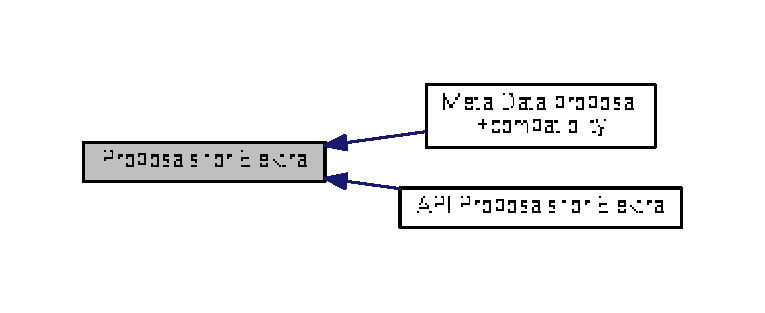
\includegraphics[width=350pt]{group__proposal}
\end{center}
\end{figure}
\subsection*{Modules}
\begin{DoxyCompactItemize}
\item 
\hyperlink{group__api}{A\+P\+I Proposals for Elektra}
\begin{DoxyCompactList}\small\item\em for kdb.\+h. \end{DoxyCompactList}\item 
\hyperlink{group__meta}{Meta Data proposal+compatibility}
\begin{DoxyCompactList}\small\item\em Meta data proposal+compatibility methods. \end{DoxyCompactList}\end{DoxyCompactItemize}
\subsection*{Enumerations}
\begin{DoxyCompactItemize}
\item 
\mbox{\Hypertarget{group__proposal_ga824e384e248ed1e05448294bff7271c0}\label{group__proposal_ga824e384e248ed1e05448294bff7271c0}} 
enum \hyperlink{group__proposal_ga824e384e248ed1e05448294bff7271c0}{elektra\+Lock\+Options} \begin{DoxyCompactList}\small\item\em Lock options. \end{DoxyCompactList}
\item 
enum \hyperlink{group__proposal_ga93673533c4c8eb1fdfca76b98c5f49b0}{elektra\+Lookup\+Options} \{ \newline
\hyperlink{group__proposal_gga93673533c4c8eb1fdfca76b98c5f49b0a187bc7e52493fb8f1eb5693015478dae}{K\+D\+B\+\_\+\+O\+\_\+\+S\+P\+EC} = 1 $<$$<$ 15, 
\hyperlink{group__proposal_gga93673533c4c8eb1fdfca76b98c5f49b0a72155bedec545b2e96372ab28169620a}{K\+D\+B\+\_\+\+O\+\_\+\+C\+R\+E\+A\+TE} = 1 $<$$<$ 16, 
\hyperlink{group__proposal_gga93673533c4c8eb1fdfca76b98c5f49b0abc4c6e04823b6d684f4db8df3b84f326}{K\+D\+B\+\_\+\+O\+\_\+\+N\+O\+C\+A\+S\+C\+A\+D\+I\+NG} = 1 $<$$<$ 17, 
\hyperlink{group__proposal_gga93673533c4c8eb1fdfca76b98c5f49b0a420d8ea3671ffea4fe8400570cfe5c8d}{K\+D\+B\+\_\+\+O\+\_\+\+N\+O\+S\+P\+EC} = 1 $<$$<$ 18, 
\newline
\hyperlink{group__proposal_gga93673533c4c8eb1fdfca76b98c5f49b0abdcfd6d28200b5c650615fba430496bb}{K\+D\+B\+\_\+\+O\+\_\+\+N\+O\+D\+E\+F\+A\+U\+LT} = 1 $<$$<$ 19, 
\hyperlink{group__proposal_gga93673533c4c8eb1fdfca76b98c5f49b0a70ac5d04d6f855e17e4c33dfeeddd39e}{K\+D\+B\+\_\+\+O\+\_\+\+C\+A\+L\+L\+B\+A\+CK} = 1 $<$$<$ 20, 
\hyperlink{group__proposal_gga93673533c4c8eb1fdfca76b98c5f49b0afe9f6ff6e374540baf600a918b07ee6e}{K\+D\+B\+\_\+\+O\+\_\+\+O\+P\+M\+P\+HM} = 1 $<$$<$ 21
 \}\begin{DoxyCompactList}\small\item\em More lookup options. \end{DoxyCompactList}
\end{DoxyCompactItemize}


\subsection{Detailed Description}
Might be added to, changed or removed from future Elektra releases. 



\subsection{Enumeration Type Documentation}
\mbox{\Hypertarget{group__proposal_ga93673533c4c8eb1fdfca76b98c5f49b0}\label{group__proposal_ga93673533c4c8eb1fdfca76b98c5f49b0}} 
\index{Proposals for Elektra@{Proposals for Elektra}!elektra\+Lookup\+Options@{elektra\+Lookup\+Options}}
\index{elektra\+Lookup\+Options@{elektra\+Lookup\+Options}!Proposals for Elektra@{Proposals for Elektra}}
\subsubsection{\texorpdfstring{elektra\+Lookup\+Options}{elektraLookupOptions}}
{\footnotesize\ttfamily enum \hyperlink{group__proposal_ga93673533c4c8eb1fdfca76b98c5f49b0}{elektra\+Lookup\+Options}}



More lookup options. 

\begin{DoxyEnumFields}{Enumerator}
\raisebox{\heightof{T}}[0pt][0pt]{\index{K\+D\+B\+\_\+\+O\+\_\+\+S\+P\+EC@{K\+D\+B\+\_\+\+O\+\_\+\+S\+P\+EC}!Proposals for Elektra@{Proposals for Elektra}}\index{Proposals for Elektra@{Proposals for Elektra}!K\+D\+B\+\_\+\+O\+\_\+\+S\+P\+EC@{K\+D\+B\+\_\+\+O\+\_\+\+S\+P\+EC}}}\mbox{\Hypertarget{group__proposal_gga93673533c4c8eb1fdfca76b98c5f49b0a187bc7e52493fb8f1eb5693015478dae}\label{group__proposal_gga93673533c4c8eb1fdfca76b98c5f49b0a187bc7e52493fb8f1eb5693015478dae}} 
K\+D\+B\+\_\+\+O\+\_\+\+S\+P\+EC&Use the passed key as specification, instead of looking up the specification first. \\
\hline

\raisebox{\heightof{T}}[0pt][0pt]{\index{K\+D\+B\+\_\+\+O\+\_\+\+C\+R\+E\+A\+TE@{K\+D\+B\+\_\+\+O\+\_\+\+C\+R\+E\+A\+TE}!Proposals for Elektra@{Proposals for Elektra}}\index{Proposals for Elektra@{Proposals for Elektra}!K\+D\+B\+\_\+\+O\+\_\+\+C\+R\+E\+A\+TE@{K\+D\+B\+\_\+\+O\+\_\+\+C\+R\+E\+A\+TE}}}\mbox{\Hypertarget{group__proposal_gga93673533c4c8eb1fdfca76b98c5f49b0a72155bedec545b2e96372ab28169620a}\label{group__proposal_gga93673533c4c8eb1fdfca76b98c5f49b0a72155bedec545b2e96372ab28169620a}} 
K\+D\+B\+\_\+\+O\+\_\+\+C\+R\+E\+A\+TE&Create the key if it was not found. \\
\hline

\raisebox{\heightof{T}}[0pt][0pt]{\index{K\+D\+B\+\_\+\+O\+\_\+\+N\+O\+C\+A\+S\+C\+A\+D\+I\+NG@{K\+D\+B\+\_\+\+O\+\_\+\+N\+O\+C\+A\+S\+C\+A\+D\+I\+NG}!Proposals for Elektra@{Proposals for Elektra}}\index{Proposals for Elektra@{Proposals for Elektra}!K\+D\+B\+\_\+\+O\+\_\+\+N\+O\+C\+A\+S\+C\+A\+D\+I\+NG@{K\+D\+B\+\_\+\+O\+\_\+\+N\+O\+C\+A\+S\+C\+A\+D\+I\+NG}}}\mbox{\Hypertarget{group__proposal_gga93673533c4c8eb1fdfca76b98c5f49b0abc4c6e04823b6d684f4db8df3b84f326}\label{group__proposal_gga93673533c4c8eb1fdfca76b98c5f49b0abc4c6e04823b6d684f4db8df3b84f326}} 
K\+D\+B\+\_\+\+O\+\_\+\+N\+O\+C\+A\+S\+C\+A\+D\+I\+NG&Disable cascading search for keys starting with /. \\
\hline

\raisebox{\heightof{T}}[0pt][0pt]{\index{K\+D\+B\+\_\+\+O\+\_\+\+N\+O\+S\+P\+EC@{K\+D\+B\+\_\+\+O\+\_\+\+N\+O\+S\+P\+EC}!Proposals for Elektra@{Proposals for Elektra}}\index{Proposals for Elektra@{Proposals for Elektra}!K\+D\+B\+\_\+\+O\+\_\+\+N\+O\+S\+P\+EC@{K\+D\+B\+\_\+\+O\+\_\+\+N\+O\+S\+P\+EC}}}\mbox{\Hypertarget{group__proposal_gga93673533c4c8eb1fdfca76b98c5f49b0a420d8ea3671ffea4fe8400570cfe5c8d}\label{group__proposal_gga93673533c4c8eb1fdfca76b98c5f49b0a420d8ea3671ffea4fe8400570cfe5c8d}} 
K\+D\+B\+\_\+\+O\+\_\+\+N\+O\+S\+P\+EC&Do not use specification for cascading keys (internal) \\
\hline

\raisebox{\heightof{T}}[0pt][0pt]{\index{K\+D\+B\+\_\+\+O\+\_\+\+N\+O\+D\+E\+F\+A\+U\+LT@{K\+D\+B\+\_\+\+O\+\_\+\+N\+O\+D\+E\+F\+A\+U\+LT}!Proposals for Elektra@{Proposals for Elektra}}\index{Proposals for Elektra@{Proposals for Elektra}!K\+D\+B\+\_\+\+O\+\_\+\+N\+O\+D\+E\+F\+A\+U\+LT@{K\+D\+B\+\_\+\+O\+\_\+\+N\+O\+D\+E\+F\+A\+U\+LT}}}\mbox{\Hypertarget{group__proposal_gga93673533c4c8eb1fdfca76b98c5f49b0abdcfd6d28200b5c650615fba430496bb}\label{group__proposal_gga93673533c4c8eb1fdfca76b98c5f49b0abdcfd6d28200b5c650615fba430496bb}} 
K\+D\+B\+\_\+\+O\+\_\+\+N\+O\+D\+E\+F\+A\+U\+LT&Do not honor the default spec (internal) \\
\hline

\raisebox{\heightof{T}}[0pt][0pt]{\index{K\+D\+B\+\_\+\+O\+\_\+\+C\+A\+L\+L\+B\+A\+CK@{K\+D\+B\+\_\+\+O\+\_\+\+C\+A\+L\+L\+B\+A\+CK}!Proposals for Elektra@{Proposals for Elektra}}\index{Proposals for Elektra@{Proposals for Elektra}!K\+D\+B\+\_\+\+O\+\_\+\+C\+A\+L\+L\+B\+A\+CK@{K\+D\+B\+\_\+\+O\+\_\+\+C\+A\+L\+L\+B\+A\+CK}}}\mbox{\Hypertarget{group__proposal_gga93673533c4c8eb1fdfca76b98c5f49b0a70ac5d04d6f855e17e4c33dfeeddd39e}\label{group__proposal_gga93673533c4c8eb1fdfca76b98c5f49b0a70ac5d04d6f855e17e4c33dfeeddd39e}} 
K\+D\+B\+\_\+\+O\+\_\+\+C\+A\+L\+L\+B\+A\+CK&For spec/ lookups that traverse deeper into hierarchy (callback in \hyperlink{group__keyset_gaa34fc43a081e6b01e4120daa6c112004}{ks\+Lookup()}) \\
\hline

\raisebox{\heightof{T}}[0pt][0pt]{\index{K\+D\+B\+\_\+\+O\+\_\+\+O\+P\+M\+P\+HM@{K\+D\+B\+\_\+\+O\+\_\+\+O\+P\+M\+P\+HM}!Proposals for Elektra@{Proposals for Elektra}}\index{Proposals for Elektra@{Proposals for Elektra}!K\+D\+B\+\_\+\+O\+\_\+\+O\+P\+M\+P\+HM@{K\+D\+B\+\_\+\+O\+\_\+\+O\+P\+M\+P\+HM}}}\mbox{\Hypertarget{group__proposal_gga93673533c4c8eb1fdfca76b98c5f49b0afe9f6ff6e374540baf600a918b07ee6e}\label{group__proposal_gga93673533c4c8eb1fdfca76b98c5f49b0afe9f6ff6e374540baf600a918b07ee6e}} 
K\+D\+B\+\_\+\+O\+\_\+\+O\+P\+M\+P\+HM&Use O\+P\+M\+P\+HM for lookup, make sure to set E\+N\+A\+B\+L\+E\+\_\+\+O\+P\+T\+I\+M\+I\+Z\+A\+T\+I\+O\+NS=ON at cmake. \\
\hline

\end{DoxyEnumFields}

\hypertarget{group__keyvalue}{}\section{Value Manipulation Methods}
\label{group__keyvalue}\index{Value Manipulation Methods@{Value Manipulation Methods}}


Methods to do various operations on Key values.  


Collaboration diagram for Value Manipulation Methods\+:
\nopagebreak
\begin{figure}[H]
\begin{center}
\leavevmode
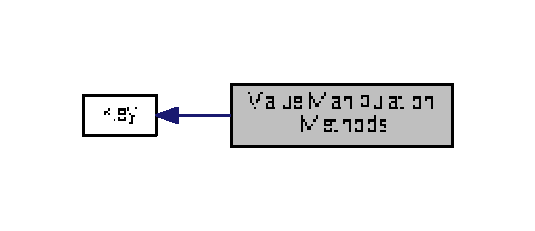
\includegraphics[width=249pt]{group__keyvalue}
\end{center}
\end{figure}
\subsection*{Functions}
\begin{DoxyCompactItemize}
\item 
const void $\ast$ \hyperlink{group__keyvalue_ga6f29609c5da53c6dc26a98678d5752af}{key\+Value} (const Key $\ast$key)
\begin{DoxyCompactList}\small\item\em Return a pointer to the real internal {\ttfamily key} value. \end{DoxyCompactList}\item 
const char $\ast$ \hyperlink{group__keyvalue_ga880936f2481d28e6e2acbe7486a21d05}{key\+String} (const Key $\ast$key)
\begin{DoxyCompactList}\small\item\em Get the c-\/string representing the value. \end{DoxyCompactList}\item 
ssize\+\_\+t \hyperlink{group__keyvalue_gae326672fffb7474abfe9baf53b73217e}{key\+Get\+Value\+Size} (const Key $\ast$key)
\begin{DoxyCompactList}\small\item\em Returns the number of bytes needed to store the key value, including the N\+U\+LL terminator. \end{DoxyCompactList}\item 
ssize\+\_\+t \hyperlink{group__keyvalue_ga41b9fac5ccddafe407fc0ae1e2eb8778}{key\+Get\+String} (const Key $\ast$key, char $\ast$returned\+String, size\+\_\+t max\+Size)
\begin{DoxyCompactList}\small\item\em Get the value of a key as a string. \end{DoxyCompactList}\item 
ssize\+\_\+t \hyperlink{group__keyvalue_ga622bde1eb0e0c4994728331326340ef2}{key\+Set\+String} (Key $\ast$key, const char $\ast$new\+String\+Value)
\begin{DoxyCompactList}\small\item\em Set the value for {\ttfamily key} as {\ttfamily new\+String\+Value}. \end{DoxyCompactList}\item 
ssize\+\_\+t \hyperlink{group__keyvalue_ga4c0d8a4a11174197699c231e0b5c3c84}{key\+Get\+Binary} (const Key $\ast$key, void $\ast$returned\+Binary, size\+\_\+t max\+Size)
\begin{DoxyCompactList}\small\item\em Get the value of a key as a binary. \end{DoxyCompactList}\item 
ssize\+\_\+t \hyperlink{group__keyvalue_gaa50a5358fd328d373a45f395fa1b99e7}{key\+Set\+Binary} (Key $\ast$key, const void $\ast$new\+Binary, size\+\_\+t data\+Size)
\begin{DoxyCompactList}\small\item\em Set the value of a key as a binary. \end{DoxyCompactList}\end{DoxyCompactItemize}


\subsection{Detailed Description}
Methods to do various operations on Key values. 

A key can contain a value in different format. The most likely situation is, that the value is interpreted as text. Use \hyperlink{group__keyvalue_ga41b9fac5ccddafe407fc0ae1e2eb8778}{key\+Get\+String()} for that. You can save any Unicode Symbols and Elektra will take care that you get the same back, independent of your current environment.

In some situations this idea fails. When you need exactly the same value back without any interpretation of the characters, there is \hyperlink{group__keyvalue_gaa50a5358fd328d373a45f395fa1b99e7}{key\+Set\+Binary()}. If you use that, its very likely that your Configuration is not according to the standard. Also for Numbers, Booleans and Date you should use \hyperlink{group__keyvalue_ga41b9fac5ccddafe407fc0ae1e2eb8778}{key\+Get\+String()}. To do so, you might use strtod() strtol() and then atol() or atof() to convert back.

To use them\+: 
\begin{DoxyCode}
\textcolor{preprocessor}{#include <kdb.h>}
\end{DoxyCode}
 

\subsection{Function Documentation}
\mbox{\Hypertarget{group__keyvalue_ga4c0d8a4a11174197699c231e0b5c3c84}\label{group__keyvalue_ga4c0d8a4a11174197699c231e0b5c3c84}} 
\index{Value Manipulation Methods@{Value Manipulation Methods}!key\+Get\+Binary@{key\+Get\+Binary}}
\index{key\+Get\+Binary@{key\+Get\+Binary}!Value Manipulation Methods@{Value Manipulation Methods}}
\subsubsection{\texorpdfstring{key\+Get\+Binary()}{keyGetBinary()}}
{\footnotesize\ttfamily ssize\+\_\+t key\+Get\+Binary (\begin{DoxyParamCaption}\item[{const Key $\ast$}]{key,  }\item[{void $\ast$}]{returned\+Binary,  }\item[{size\+\_\+t}]{max\+Size }\end{DoxyParamCaption})}



Get the value of a key as a binary. 

If the type is not binary -\/1 will be returned.

When the binary data is empty (this is not the same as \char`\"{}\char`\"{}!) 0 will be returned and the returned\+Binary will not be changed.

For string values see \hyperlink{group__keyvalue_ga41b9fac5ccddafe407fc0ae1e2eb8778}{key\+Get\+String()} and \hyperlink{group__keytest_gaea7670778abd07fee0fe8ac12a149190}{key\+Is\+String()}.

When the returned\+Binary is to small to hold the data (its maximum size is given by max\+Size), the returned\+Binary will not be changed and -\/1 is returned.

\begin{DoxyParagraph}{Example\+:}

\begin{DoxyCode}
Key *key = \hyperlink{group__key_gad23c65b44bf48d773759e1f9a4d43b89}{keyNew} (\textcolor{stringliteral}{"user/keyname"}, KEY\_TYPE, KEY\_TYPE\_BINARY, \hyperlink{group__key_gga91fb3178848bd682000958089abbaf40aa8adb6fcb92dec58fb19410eacfdd403}{KEY\_END});
\textcolor{keywordtype}{char} buffer[300];

\textcolor{keywordflow}{if} (\hyperlink{group__keyvalue_ga4c0d8a4a11174197699c231e0b5c3c84}{keyGetBinary}(key,buffer,\textcolor{keyword}{sizeof}(buffer)) == -1)
\{
        \textcolor{comment}{// handle error}
\}
\end{DoxyCode}

\end{DoxyParagraph}

\begin{DoxyParams}{Parameters}
{\em key} & the object to gather the value from \\
\hline
{\em returned\+Binary} & pre-\/allocated memory to store a copy of the key value \\
\hline
{\em max\+Size} & number of bytes of pre-\/allocated memory in {\ttfamily returned\+Binary} \\
\hline
\end{DoxyParams}
\begin{DoxyReturn}{Returns}
the number of bytes actually copied to {\ttfamily returned\+Binary} 
\end{DoxyReturn}

\begin{DoxyRetVals}{Return values}
{\em 0} & if the binary is empty \\
\hline
{\em -\/1} & on N\+U\+LL pointers \\
\hline
{\em -\/1} & if max\+Size is 0 \\
\hline
{\em -\/1} & if max\+Size is too small for string \\
\hline
{\em -\/1} & if max\+Size is larger than S\+S\+I\+Z\+E\+\_\+\+M\+AX \\
\hline
{\em -\/1} & on type mismatch\+: binary expected, but found string \\
\hline
\end{DoxyRetVals}
\begin{DoxySeeAlso}{See also}
\hyperlink{group__keyvalue_ga6f29609c5da53c6dc26a98678d5752af}{key\+Value()}, \hyperlink{group__keyvalue_gae326672fffb7474abfe9baf53b73217e}{key\+Get\+Value\+Size()}, \hyperlink{group__keyvalue_gaa50a5358fd328d373a45f395fa1b99e7}{key\+Set\+Binary()} 

\hyperlink{group__keyvalue_ga41b9fac5ccddafe407fc0ae1e2eb8778}{key\+Get\+String()} and \hyperlink{group__keyvalue_ga622bde1eb0e0c4994728331326340ef2}{key\+Set\+String()} as preferred alternative to binary 

\hyperlink{group__keytest_ga9526b371087564e43e3dff8ad0dac949}{key\+Is\+Binary()} to see how to check for binary type 
\end{DoxySeeAlso}
\mbox{\Hypertarget{group__keyvalue_ga41b9fac5ccddafe407fc0ae1e2eb8778}\label{group__keyvalue_ga41b9fac5ccddafe407fc0ae1e2eb8778}} 
\index{Value Manipulation Methods@{Value Manipulation Methods}!key\+Get\+String@{key\+Get\+String}}
\index{key\+Get\+String@{key\+Get\+String}!Value Manipulation Methods@{Value Manipulation Methods}}
\subsubsection{\texorpdfstring{key\+Get\+String()}{keyGetString()}}
{\footnotesize\ttfamily ssize\+\_\+t key\+Get\+String (\begin{DoxyParamCaption}\item[{const Key $\ast$}]{key,  }\item[{char $\ast$}]{returned\+String,  }\item[{size\+\_\+t}]{max\+Size }\end{DoxyParamCaption})}



Get the value of a key as a string. 

When there is no value inside the string, 1 will be returned and the returned\+String will be empty \char`\"{}\char`\"{} to avoid programming errors that old strings are shown to the user.

For binary values see \hyperlink{group__keyvalue_ga4c0d8a4a11174197699c231e0b5c3c84}{key\+Get\+Binary()} and \hyperlink{group__keytest_ga9526b371087564e43e3dff8ad0dac949}{key\+Is\+Binary()}.

\begin{DoxyParagraph}{Example\+:}

\begin{DoxyCode}
Key *key = \hyperlink{group__key_gad23c65b44bf48d773759e1f9a4d43b89}{keyNew} (\textcolor{stringliteral}{"user/keyname"}, \hyperlink{group__key_gga91fb3178848bd682000958089abbaf40aa8adb6fcb92dec58fb19410eacfdd403}{KEY\_END});
\textcolor{keywordtype}{char} buffer[300];

\textcolor{keywordflow}{if} (\hyperlink{group__keyvalue_ga41b9fac5ccddafe407fc0ae1e2eb8778}{keyGetString}(key,buffer,\textcolor{keyword}{sizeof}(buffer)) == -1)
\{
        \textcolor{comment}{// handle error}
\} \textcolor{keywordflow}{else} \{
        printf (\textcolor{stringliteral}{"buffer: %s\(\backslash\)n"}, buffer);
\}
\end{DoxyCode}

\end{DoxyParagraph}

\begin{DoxyParams}{Parameters}
{\em key} & the object to gather the value from \\
\hline
{\em returned\+String} & pre-\/allocated memory to store a copy of the key value \\
\hline
{\em max\+Size} & number of bytes of allocated memory in {\ttfamily returned\+String} \\
\hline
\end{DoxyParams}
\begin{DoxyReturn}{Returns}
the number of bytes actually copied to {\ttfamily returned\+String}, including final N\+U\+LL 
\end{DoxyReturn}

\begin{DoxyRetVals}{Return values}
{\em 1} & if the string is empty \\
\hline
{\em -\/1} & on any N\+U\+LL pointers \\
\hline
{\em -\/1} & on type mismatch\+: string expected, but found binary \\
\hline
{\em -\/1} & max\+Size is 0 \\
\hline
{\em -\/1} & if max\+Size is too small for string \\
\hline
{\em -\/1} & if max\+Size is larger than S\+S\+I\+Z\+E\+\_\+\+M\+AX \\
\hline
\end{DoxyRetVals}
\begin{DoxySeeAlso}{See also}
\hyperlink{group__keyvalue_ga6f29609c5da53c6dc26a98678d5752af}{key\+Value()}, \hyperlink{group__keyvalue_gae326672fffb7474abfe9baf53b73217e}{key\+Get\+Value\+Size()}, \hyperlink{group__keyvalue_ga622bde1eb0e0c4994728331326340ef2}{key\+Set\+String()}, \hyperlink{group__keyvalue_ga880936f2481d28e6e2acbe7486a21d05}{key\+String()} 

\hyperlink{group__keyvalue_ga4c0d8a4a11174197699c231e0b5c3c84}{key\+Get\+Binary()} for working with binary data 
\end{DoxySeeAlso}
\mbox{\Hypertarget{group__keyvalue_gae326672fffb7474abfe9baf53b73217e}\label{group__keyvalue_gae326672fffb7474abfe9baf53b73217e}} 
\index{Value Manipulation Methods@{Value Manipulation Methods}!key\+Get\+Value\+Size@{key\+Get\+Value\+Size}}
\index{key\+Get\+Value\+Size@{key\+Get\+Value\+Size}!Value Manipulation Methods@{Value Manipulation Methods}}
\subsubsection{\texorpdfstring{key\+Get\+Value\+Size()}{keyGetValueSize()}}
{\footnotesize\ttfamily ssize\+\_\+t key\+Get\+Value\+Size (\begin{DoxyParamCaption}\item[{const Key $\ast$}]{key }\end{DoxyParamCaption})}



Returns the number of bytes needed to store the key value, including the N\+U\+LL terminator. 

It returns the correct size, independent of the Key Type. If it is a binary there might be \textquotesingle{}\textbackslash{}0\textquotesingle{} values in it.

For an empty string you need one byte to store the ending N\+U\+LL. For that reason 1 is returned. This is not true for binary data, so there might be returned 0 too.

A binary key has no \textquotesingle{}\textbackslash{}0\textquotesingle{} termination. String types have it, so to there length will be added 1 to have enough space to store it.

This method can be used with \hyperlink{internal_8c_a35cdc2e5caed3454cb73b4fc7f37858c}{elektra\+Malloc()} before \hyperlink{group__keyvalue_ga41b9fac5ccddafe407fc0ae1e2eb8778}{key\+Get\+String()} or \hyperlink{group__keyvalue_ga4c0d8a4a11174197699c231e0b5c3c84}{key\+Get\+Binary()} is called.


\begin{DoxyCode}
\textcolor{keywordtype}{char} *buffer;
buffer = \hyperlink{internal_8c_a35cdc2e5caed3454cb73b4fc7f37858c}{elektraMalloc} (\hyperlink{group__keyvalue_gae326672fffb7474abfe9baf53b73217e}{keyGetValueSize} (key));
\textcolor{comment}{// use this buffer to store the value (binary or string)}
\textcolor{comment}{// pass keyGetValueSize (key) for maxSize}
\end{DoxyCode}



\begin{DoxyParams}{Parameters}
{\em key} & the key object to work with \\
\hline
\end{DoxyParams}
\begin{DoxyReturn}{Returns}
the number of bytes needed to store the key value 
\end{DoxyReturn}

\begin{DoxyRetVals}{Return values}
{\em 1} & when there is no data and type is not binary \\
\hline
{\em 0} & when there is no data and type is binary \\
\hline
{\em -\/1} & on null pointer \\
\hline
\end{DoxyRetVals}
\begin{DoxySeeAlso}{See also}
\hyperlink{group__keyvalue_ga41b9fac5ccddafe407fc0ae1e2eb8778}{key\+Get\+String()}, \hyperlink{group__keyvalue_ga4c0d8a4a11174197699c231e0b5c3c84}{key\+Get\+Binary()}, \hyperlink{group__keyvalue_ga6f29609c5da53c6dc26a98678d5752af}{key\+Value()} 
\end{DoxySeeAlso}
\mbox{\Hypertarget{group__keyvalue_gaa50a5358fd328d373a45f395fa1b99e7}\label{group__keyvalue_gaa50a5358fd328d373a45f395fa1b99e7}} 
\index{Value Manipulation Methods@{Value Manipulation Methods}!key\+Set\+Binary@{key\+Set\+Binary}}
\index{key\+Set\+Binary@{key\+Set\+Binary}!Value Manipulation Methods@{Value Manipulation Methods}}
\subsubsection{\texorpdfstring{key\+Set\+Binary()}{keySetBinary()}}
{\footnotesize\ttfamily ssize\+\_\+t key\+Set\+Binary (\begin{DoxyParamCaption}\item[{Key $\ast$}]{key,  }\item[{const void $\ast$}]{new\+Binary,  }\item[{size\+\_\+t}]{data\+Size }\end{DoxyParamCaption})}



Set the value of a key as a binary. 

A private copy of {\ttfamily new\+Binary} will allocated and saved inside {\ttfamily key}, so the parameter can be deallocated after the call.

Binary values might be encoded in another way then string values depending on the plugin. Typically character encodings should not take place on binary data. Consider using a string key instead.

When new\+Binary is a N\+U\+LL pointer the binary will be freed and 0 will be returned.

\begin{DoxyNote}{Note}
The metadata \char`\"{}binary\char`\"{} will be set to mark that the key is binary from now on. When the key is already binary the metadata won\textquotesingle{}t be changed. This will only happen in the successful case, but not when -\/1 is returned.
\end{DoxyNote}

\begin{DoxyParams}{Parameters}
{\em key} & the object on which to set the value \\
\hline
{\em new\+Binary} & is a pointer to any binary data or N\+U\+LL to free the previous set data \\
\hline
{\em data\+Size} & number of bytes to copy from {\ttfamily new\+Binary} \\
\hline
\end{DoxyParams}
\begin{DoxyReturn}{Returns}
the number of bytes actually copied to internal struct storage 
\end{DoxyReturn}

\begin{DoxyRetVals}{Return values}
{\em 0} & when the internal binary was freed and is now a null pointer \\
\hline
{\em -\/1} & if key is a N\+U\+LL pointer \\
\hline
{\em -\/1} & when data\+Size is 0 (but new\+Binary not N\+U\+LL) or larger than S\+S\+I\+Z\+E\+\_\+\+M\+AX \\
\hline
\end{DoxyRetVals}
\begin{DoxySeeAlso}{See also}
\hyperlink{group__keyvalue_ga4c0d8a4a11174197699c231e0b5c3c84}{key\+Get\+Binary()} 

\hyperlink{group__keytest_ga9526b371087564e43e3dff8ad0dac949}{key\+Is\+Binary()} to check if the type is binary 

\hyperlink{group__keyvalue_ga41b9fac5ccddafe407fc0ae1e2eb8778}{key\+Get\+String()} and \hyperlink{group__keyvalue_ga622bde1eb0e0c4994728331326340ef2}{key\+Set\+String()} as preferred alternative to binary 
\end{DoxySeeAlso}
\mbox{\Hypertarget{group__keyvalue_ga622bde1eb0e0c4994728331326340ef2}\label{group__keyvalue_ga622bde1eb0e0c4994728331326340ef2}} 
\index{Value Manipulation Methods@{Value Manipulation Methods}!key\+Set\+String@{key\+Set\+String}}
\index{key\+Set\+String@{key\+Set\+String}!Value Manipulation Methods@{Value Manipulation Methods}}
\subsubsection{\texorpdfstring{key\+Set\+String()}{keySetString()}}
{\footnotesize\ttfamily ssize\+\_\+t key\+Set\+String (\begin{DoxyParamCaption}\item[{Key $\ast$}]{key,  }\item[{const char $\ast$}]{new\+String\+Value }\end{DoxyParamCaption})}



Set the value for {\ttfamily key} as {\ttfamily new\+String\+Value}. 

The function will allocate and save a private copy of {\ttfamily new\+String\+Value}, so the parameter can be freed after the call.

String values will be saved in backend storage, when kdb\+Set\+Key() will be called, in U\+T\+F-\/8 universal encoding, regardless of the program\textquotesingle{}s current encoding, when iconv plugin is present.

\begin{DoxyNote}{Note}
The type will be set to K\+E\+Y\+\_\+\+T\+Y\+P\+E\+\_\+\+S\+T\+R\+I\+NG. When the type of the key is already a string type it won\textquotesingle{}t be changed.
\end{DoxyNote}

\begin{DoxyParams}{Parameters}
{\em key} & the key to set the string value \\
\hline
{\em new\+String\+Value} & N\+U\+L\+L-\/terminated text string to be set as {\ttfamily key\textquotesingle{}s} value \\
\hline
\end{DoxyParams}
\begin{DoxyReturn}{Returns}
the number of bytes actually saved in private struct including final N\+U\+LL 
\end{DoxyReturn}

\begin{DoxyRetVals}{Return values}
{\em 1} & if new\+String\+Value is a N\+U\+LL pointer, this will make the string empty (string only containing null termination) \\
\hline
{\em -\/1} & if key is a N\+U\+LL pointer \\
\hline
\end{DoxyRetVals}
\begin{DoxySeeAlso}{See also}
\hyperlink{group__keyvalue_ga41b9fac5ccddafe407fc0ae1e2eb8778}{key\+Get\+String()}, \hyperlink{group__keyvalue_ga6f29609c5da53c6dc26a98678d5752af}{key\+Value()}, \hyperlink{group__keyvalue_ga880936f2481d28e6e2acbe7486a21d05}{key\+String()} 
\end{DoxySeeAlso}
\mbox{\Hypertarget{group__keyvalue_ga880936f2481d28e6e2acbe7486a21d05}\label{group__keyvalue_ga880936f2481d28e6e2acbe7486a21d05}} 
\index{Value Manipulation Methods@{Value Manipulation Methods}!key\+String@{key\+String}}
\index{key\+String@{key\+String}!Value Manipulation Methods@{Value Manipulation Methods}}
\subsubsection{\texorpdfstring{key\+String()}{keyString()}}
{\footnotesize\ttfamily const char$\ast$ key\+String (\begin{DoxyParamCaption}\item[{const Key $\ast$}]{key }\end{DoxyParamCaption})}



Get the c-\/string representing the value. 

Will return (null) on null pointers. Will return (binary) on binary data not ended with a null byte.

It is not checked if it is actually a string, only if it terminates for security reasons.

\begin{DoxyReturn}{Returns}
the c-\/string of the value 
\end{DoxyReturn}

\begin{DoxyRetVals}{Return values}
{\em (null)} & on null keys \\
\hline
{\em \char`\"{}\char`\"{}} & if no data found \\
\hline
{\em (binary)} & on binary keys\\
\hline
\end{DoxyRetVals}

\begin{DoxyParams}{Parameters}
{\em key} & the key object to get the string from \\
\hline
\end{DoxyParams}
\mbox{\Hypertarget{group__keyvalue_ga6f29609c5da53c6dc26a98678d5752af}\label{group__keyvalue_ga6f29609c5da53c6dc26a98678d5752af}} 
\index{Value Manipulation Methods@{Value Manipulation Methods}!key\+Value@{key\+Value}}
\index{key\+Value@{key\+Value}!Value Manipulation Methods@{Value Manipulation Methods}}
\subsubsection{\texorpdfstring{key\+Value()}{keyValue()}}
{\footnotesize\ttfamily const void$\ast$ key\+Value (\begin{DoxyParamCaption}\item[{const Key $\ast$}]{key }\end{DoxyParamCaption})}



Return a pointer to the real internal {\ttfamily key} value. 

This is a much more efficient version of \hyperlink{group__keyvalue_ga41b9fac5ccddafe407fc0ae1e2eb8778}{key\+Get\+String()} \hyperlink{group__keyvalue_ga4c0d8a4a11174197699c231e0b5c3c84}{key\+Get\+Binary()}, and you should use it if you are responsible enough to not mess up things. You are not allowed to modify anything in the returned string. If you need a copy of the Value, consider to use \hyperlink{group__keyvalue_ga41b9fac5ccddafe407fc0ae1e2eb8778}{key\+Get\+String()} or \hyperlink{group__keyvalue_ga4c0d8a4a11174197699c231e0b5c3c84}{key\+Get\+Binary()} instead.\hypertarget{group__keyvalue_string}{}\subsection{String Handling}\label{group__keyvalue_string}
If {\ttfamily key} is string (\hyperlink{group__keytest_gaea7670778abd07fee0fe8ac12a149190}{key\+Is\+String()}), you may cast the returned as a {\ttfamily \char`\"{}char $\ast$\char`\"{}} because you\textquotesingle{}ll get a N\+U\+LL terminated regular string.

\hyperlink{group__keyvalue_ga6f29609c5da53c6dc26a98678d5752af}{key\+Value()} returns \char`\"{}\char`\"{} in string mode when there is no value. The reason is 
\begin{DoxyCode}
key=\hyperlink{group__key_gad23c65b44bf48d773759e1f9a4d43b89}{keyNew}(0);
\hyperlink{group__keyvalue_ga622bde1eb0e0c4994728331326340ef2}{keySetString}(key,\textcolor{stringliteral}{""});
\hyperlink{group__keyvalue_ga6f29609c5da53c6dc26a98678d5752af}{keyValue}(key); \textcolor{comment}{// you would expect "" here}
\hyperlink{group__key_ga3df95bbc2494e3e6703ece5639be5bb1}{keyDel}(key);
\end{DoxyCode}
\hypertarget{group__keyvalue_binary}{}\subsection{Binary Data Handling}\label{group__keyvalue_binary}
If the data is binary, the size of the value must be determined by \hyperlink{group__keyvalue_gae326672fffb7474abfe9baf53b73217e}{key\+Get\+Value\+Size()}, any strlen() operations are not suitable to determine the size.

\hyperlink{group__keyvalue_ga6f29609c5da53c6dc26a98678d5752af}{key\+Value()} returns 0 in binary mode when there is no value. The reason is 
\begin{DoxyCode}
key=\hyperlink{group__key_gad23c65b44bf48d773759e1f9a4d43b89}{keyNew}(0);
\hyperlink{group__keyvalue_gaa50a5358fd328d373a45f395fa1b99e7}{keySetBinary}(key, 0, 0);
\hyperlink{group__keyvalue_ga6f29609c5da53c6dc26a98678d5752af}{keyValue}(key); \textcolor{comment}{// you would expect 0 here}

\hyperlink{group__keyvalue_gaa50a5358fd328d373a45f395fa1b99e7}{keySetBinary}(key,\textcolor{stringliteral}{""}, 1);
\hyperlink{group__keyvalue_ga6f29609c5da53c6dc26a98678d5752af}{keyValue}(key); \textcolor{comment}{// you would expect "" (a pointer to '\(\backslash\)0') here}

\textcolor{keywordtype}{int} i=23;
\hyperlink{group__keyvalue_gaa50a5358fd328d373a45f395fa1b99e7}{keySetBinary}(key, (\textcolor{keywordtype}{void}*)&i, 4);
(\textcolor{keywordtype}{int}*)\hyperlink{group__keyvalue_ga6f29609c5da53c6dc26a98678d5752af}{keyValue}(key); \textcolor{comment}{// you would expect a pointer to (int)23 here}
\hyperlink{group__key_ga3df95bbc2494e3e6703ece5639be5bb1}{keyDel}(key);
\end{DoxyCode}


\begin{DoxyNote}{Note}
Note that the Key structure keeps its own size field that is calculated by library internal calls, so to avoid inconsistencies, you must never use the pointer returned by \hyperlink{group__keyvalue_ga6f29609c5da53c6dc26a98678d5752af}{key\+Value()} method to set a new value. Use \hyperlink{group__keyvalue_ga622bde1eb0e0c4994728331326340ef2}{key\+Set\+String()} or \hyperlink{group__keyvalue_gaa50a5358fd328d373a45f395fa1b99e7}{key\+Set\+Binary()} instead.
\end{DoxyNote}
\begin{DoxyWarning}{Warning}
Binary keys will return a N\+U\+LL pointer when there is no data in contrast to \hyperlink{group__keyname_ga8e805c726a60da921d3736cda7813513}{key\+Name()}, \hyperlink{group__keyname_gaaff35e7ca8af5560c47e662ceb9465f5}{key\+Base\+Name()}, \hyperlink{owner_8c_af6485fb8599714b6bbd830cf915ffea5}{key\+Owner()} and \hyperlink{group__meta_gac89fd319783b3457db45b4c09e55274a}{key\+Comment()}. For string value the behaviour is the same.
\end{DoxyWarning}
\begin{DoxyParagraph}{Example\+:}

\begin{DoxyCode}
KDB *handle = \hyperlink{group__kdb_ga6808defe5870f328dd17910aacbdc6ca}{kdbOpen}();
KeySet *ks=\hyperlink{group__keyset_ga671e1aaee3ae9dc13b4834a4ddbd2c3c}{ksNew}(0, \hyperlink{kdbenum_8c_a7a28fce3773b2c873c94ac80b8b4cd54}{KS\_END});
Key *current=0;

kdbGetByName(handle,ks,\textcolor{stringliteral}{"system/sw/my"},\hyperlink{group__keyset_gga98a3d6a4016c9dad9cbd1a99a9c2a45aad9d03b36ee88ca5a774cc01b190c99b8}{KDB\_O\_SORT}|KDB\_O\_RECURSIVE);

\hyperlink{group__keyset_gabe793ff51f1728e3429c84a8a9086b70}{ksRewind}(ks);
\textcolor{keywordflow}{while} (current=\hyperlink{group__keyset_ga317321c9065b5a4b3e33fe1c399bcec9}{ksNext}(ks)) \{
        \textcolor{keywordtype}{size\_t} size=0;

        \textcolor{keywordflow}{if} (keyIsBin(current)) \{
                size=\hyperlink{group__keyvalue_gae326672fffb7474abfe9baf53b73217e}{keyGetValueSize}(current);
                printf(\textcolor{stringliteral}{"Key %s has a value of size %d bytes. Value: <BINARY>\(\backslash\)nComment: %s"},
                        \hyperlink{group__keyname_ga8e805c726a60da921d3736cda7813513}{keyName}(current),
                        size,
                        \hyperlink{group__meta_gac89fd319783b3457db45b4c09e55274a}{keyComment}(current));
        \} \textcolor{keywordflow}{else} \{
                size=\hyperlink{internal_8c_afd676487565d083a6ad5a1381095acd8}{elektraStrLen}((\textcolor{keywordtype}{char} *)\hyperlink{group__keyvalue_ga6f29609c5da53c6dc26a98678d5752af}{keyValue}(current));
                printf(\textcolor{stringliteral}{"Key %s has a value of size %d bytes. Value: %s\(\backslash\)nComment: %s"},
                        \hyperlink{group__keyname_ga8e805c726a60da921d3736cda7813513}{keyName}(current),
                        size,
                        (\textcolor{keywordtype}{char} *)\hyperlink{group__keyvalue_ga6f29609c5da53c6dc26a98678d5752af}{keyValue}(current),
                        \hyperlink{group__meta_gac89fd319783b3457db45b4c09e55274a}{keyComment}(current));
        \}
\}

\hyperlink{group__keyset_ga27e5c16473b02a422238c8d970db7ac8}{ksDel} (ks);
\hyperlink{group__kdb_gadb54dc9fda17ee07deb9444df745c96f}{kdbClose} (handle);
\end{DoxyCode}

\end{DoxyParagraph}

\begin{DoxyParams}{Parameters}
{\em key} & the key object to work with \\
\hline
\end{DoxyParams}
\begin{DoxyReturn}{Returns}
a pointer to internal value 
\end{DoxyReturn}

\begin{DoxyRetVals}{Return values}
{\em \char`\"{}\char`\"{}} & when there is no data and key is not binary \\
\hline
{\em 0} & where there is no data and key is binary \\
\hline
{\em 0} & on N\+U\+LL pointer \\
\hline
\end{DoxyRetVals}
\begin{DoxySeeAlso}{See also}
\hyperlink{group__keyvalue_gae326672fffb7474abfe9baf53b73217e}{key\+Get\+Value\+Size()}, \hyperlink{group__keyvalue_ga41b9fac5ccddafe407fc0ae1e2eb8778}{key\+Get\+String()}, \hyperlink{group__keyvalue_ga4c0d8a4a11174197699c231e0b5c3c84}{key\+Get\+Binary()} 
\end{DoxySeeAlso}

\chapter{Namespace Documentation}
\hypertarget{namespacekdb}{}\section{kdb Namespace Reference}
\label{namespacekdb}\index{kdb@{kdb}}


This is the main namespace for the C++ binding and libraries.  


\subsection*{Namespaces}
\begin{DoxyCompactItemize}
\item 
 \hyperlink{namespacekdb_1_1tools}{tools}
\begin{DoxyCompactList}\small\item\em This namespace is for the libtool library. \end{DoxyCompactList}\end{DoxyCompactItemize}
\subsection*{Classes}
\begin{DoxyCompactItemize}
\item 
struct \hyperlink{structkdb_1_1Command}{Command}
\begin{DoxyCompactList}\small\item\em Used by contexts for callbacks (to run code using a mutex). \end{DoxyCompactList}\item 
class \hyperlink{classkdb_1_1Context}{Context}
\begin{DoxyCompactList}\small\item\em Provides a context for configuration. \end{DoxyCompactList}\item 
class \hyperlink{classkdb_1_1ContextPolicyIs}{Context\+Policy\+Is}
\begin{DoxyCompactList}\small\item\em Needed by the user to set one of the policies. \end{DoxyCompactList}\item 
class \hyperlink{classkdb_1_1Coordinator}{Coordinator}
\begin{DoxyCompactList}\small\item\em Thread safe coordination of Thread\+Context per Threads. \end{DoxyCompactList}\item 
class \hyperlink{classkdb_1_1DefaultGetPolicy}{Default\+Get\+Policy}
\begin{DoxyCompactList}\small\item\em Implements lookup with spec. \end{DoxyCompactList}\item 
class \hyperlink{classkdb_1_1DefaultSetPolicy}{Default\+Set\+Policy}
\begin{DoxyCompactList}\small\item\em Implements creating user\+:/ key when key is not found. \end{DoxyCompactList}\item 
class \hyperlink{classkdb_1_1GetPolicyIs}{Get\+Policy\+Is}
\begin{DoxyCompactList}\small\item\em Needed by the user to set one of the policies. \end{DoxyCompactList}\item 
class \hyperlink{classkdb_1_1KDB}{K\+DB}
\begin{DoxyCompactList}\small\item\em Constructs a class \hyperlink{classkdb_1_1KDB}{K\+DB}. \end{DoxyCompactList}\item 
class \hyperlink{classkdb_1_1Key}{Key}
\begin{DoxyCompactList}\small\item\em \hyperlink{classkdb_1_1Key}{Key} is an essential class that encapsulates key \hyperlink{group__keyname}{name }, \hyperlink{group__keyvalue}{value } and \hyperlink{group__keymeta}{metainfo }. \end{DoxyCompactList}\item 
class \hyperlink{classkdb_1_1KeySet}{Key\+Set}
\begin{DoxyCompactList}\small\item\em A keyset holds together a set of keys. \end{DoxyCompactList}\item 
class \hyperlink{classkdb_1_1KeySetIterator}{Key\+Set\+Iterator}
\begin{DoxyCompactList}\small\item\em For C++ forward Iteration over Key\+Sets. \end{DoxyCompactList}\item 
class \hyperlink{classkdb_1_1KeySetReverseIterator}{Key\+Set\+Reverse\+Iterator}
\begin{DoxyCompactList}\small\item\em For C++ reverse Iteration over Key\+Sets. \end{DoxyCompactList}\item 
class \hyperlink{classkdb_1_1Layer}{Layer}
\begin{DoxyCompactList}\small\item\em Base class for all layers. \end{DoxyCompactList}\item 
class \hyperlink{classkdb_1_1LockPolicyIs}{Lock\+Policy\+Is}
\begin{DoxyCompactList}\small\item\em Needed by the user to set one of the policies. \end{DoxyCompactList}\item 
class \hyperlink{classkdb_1_1NameIterator}{Name\+Iterator}
\begin{DoxyCompactList}\small\item\em For C++ forward Iteration over Names. \end{DoxyCompactList}\item 
class \hyperlink{classkdb_1_1NameReverseIterator}{Name\+Reverse\+Iterator}
\begin{DoxyCompactList}\small\item\em For C++ reverse Iteration over Names. \end{DoxyCompactList}\item 
class \hyperlink{classkdb_1_1none__t}{none\+\_\+t}
\begin{DoxyCompactList}\small\item\em This type is being used as bottom type that always fails. \end{DoxyCompactList}\item 
class \hyperlink{classkdb_1_1ObserverPolicyIs}{Observer\+Policy\+Is}
\begin{DoxyCompactList}\small\item\em Needed by the user to set one of the policies. \end{DoxyCompactList}\item 
struct \hyperlink{structkdb_1_1PerContext}{Per\+Context}
\begin{DoxyCompactList}\small\item\em A data structure that is stored by context inside the \hyperlink{classkdb_1_1Coordinator}{Coordinator}. \end{DoxyCompactList}\item 
class \hyperlink{classkdb_1_1SetPolicyIs}{Set\+Policy\+Is}
\begin{DoxyCompactList}\small\item\em Needed by the user to set one of the policies. \end{DoxyCompactList}\item 
class \hyperlink{classkdb_1_1ThreadSubject}{Thread\+Subject}
\begin{DoxyCompactList}\small\item\em Subject from Observer pattern for Thread\+Context. \end{DoxyCompactList}\item 
struct \hyperlink{structkdb_1_1VaAlloc}{Va\+Alloc}
\begin{DoxyCompactList}\small\item\em Needed to avoid constructor ambiguity. \end{DoxyCompactList}\item 
class \hyperlink{classkdb_1_1ValueObserver}{Value\+Observer}
\begin{DoxyCompactList}\small\item\em Base class for values to be observed. \end{DoxyCompactList}\item 
class \hyperlink{classkdb_1_1Wrapped}{Wrapped}
\begin{DoxyCompactList}\small\item\em Everything implementing this interface can be used as layer. \end{DoxyCompactList}\item 
class \hyperlink{classkdb_1_1WritePolicyIs}{Write\+Policy\+Is}
\begin{DoxyCompactList}\small\item\em Needed by the user to set one of the policies. \end{DoxyCompactList}\end{DoxyCompactItemize}
\subsection*{Typedefs}
\begin{DoxyCompactItemize}
\item 
\mbox{\Hypertarget{namespacekdb_ac389d72a0c7be0c026628870f81148fe}\label{namespacekdb_ac389d72a0c7be0c026628870f81148fe}} 
typedef std\+::unordered\+\_\+map$<$ std\+::string, Layer\+Action $>$ \hyperlink{namespacekdb_ac389d72a0c7be0c026628870f81148fe}{Layer\+Map}
\begin{DoxyCompactList}\small\item\em A vector of layers. \end{DoxyCompactList}\end{DoxyCompactItemize}
\subsection*{Functions}
\begin{DoxyCompactItemize}
\item 
int \hyperlink{namespacekdb_afc8477f4bb768ada40b8e4b82d9fcaf0}{gopts\+Contract} (\hyperlink{classkdb_1_1KeySet}{kdb\+::\+Key\+Set} \&contract, int argc, const char $\ast$const $\ast$argv, const char $\ast$const $\ast$envp, const \hyperlink{classkdb_1_1Key}{kdb\+::\+Key} \&parent\+Key, \hyperlink{classkdb_1_1KeySet}{kdb\+::\+Key\+Set} \&gopts\+Config)
\item 
int \hyperlink{namespacekdb_a90e4547be745a211a4ad95bdd27d0254}{gopts\+Contract} (\hyperlink{classkdb_1_1KeySet}{kdb\+::\+Key\+Set} \&contract, const std\+::string \&args\+String, const std\+::string \&env\+String, const \hyperlink{classkdb_1_1Key}{kdb\+::\+Key} \&parent\+Key, \hyperlink{classkdb_1_1KeySet}{kdb\+::\+Key\+Set} \&gopts\+Config)
\begin{DoxyCompactList}\small\item\em Prefer to use gopts\+Contract with argc, argv and envp if possible (especially when you are calling this in your main function) \end{DoxyCompactList}\item 
int \hyperlink{namespacekdb_afa8d46930ac176c22c7f4e77c776d08e}{gopts\+Contract} (\hyperlink{classkdb_1_1KeySet}{kdb\+::\+Key\+Set} \&contract, const std\+::vector$<$ std\+::string $>$ \&args, const std\+::vector$<$ std\+::string $>$ \&env, const \hyperlink{classkdb_1_1Key}{kdb\+::\+Key} \&parent\+Key, \hyperlink{classkdb_1_1KeySet}{kdb\+::\+Key\+Set} \&gopts\+Config)
\begin{DoxyCompactList}\small\item\em Prefer to use gopts\+Contract with argc, argv and envp if possible (especially when you are calling this in your main function) \end{DoxyCompactList}\item 
bool \hyperlink{namespacekdb_a53a162c7ff73150a3f6e6ab9d191aab0}{operator$<$} (\hyperlink{classkdb_1_1ValueObserver}{Value\+Observer} const \&lhs, \hyperlink{classkdb_1_1ValueObserver}{Value\+Observer} const \&rhs)
\begin{DoxyCompactList}\small\item\em Needed to put a \hyperlink{classkdb_1_1ValueObserver}{Value\+Observer} in a map. \end{DoxyCompactList}\item 
std\+::ostream \& \hyperlink{namespacekdb_ac004b5ba79154cbba02d5e5d83337e47}{operator$<$$<$} (std\+::ostream \&os, \hyperlink{classkdb_1_1Key}{kdb\+::\+Key} const \&k)
\begin{DoxyCompactList}\small\item\em Stream the name of a key. \end{DoxyCompactList}\item 
std\+::istream \& \hyperlink{namespacekdb_a66342865d6cdbb19075f52d92e7a61b1}{operator$>$$>$} (std\+::istream \&is, \hyperlink{classkdb_1_1Key}{kdb\+::\+Key} \&k)
\begin{DoxyCompactList}\small\item\em Reads a line with a keys name. \end{DoxyCompactList}\item 
std\+::ostream \& \hyperlink{namespacekdb_afd28754a48d420d2f2a41c5d8242f3fb}{operator$<$$<$} (std\+::ostream \&os, \hyperlink{classkdb_1_1KeySet}{kdb\+::\+Key\+Set} const \&cks)
\begin{DoxyCompactList}\small\item\em Outputs line per line the keynames. \end{DoxyCompactList}\item 
std\+::istream \& \hyperlink{namespacekdb_ac4479a9f39ed65ffd251161bcaf8ea89}{operator$>$$>$} (std\+::istream \&is, \hyperlink{classkdb_1_1KeySet}{kdb\+::\+Key\+Set} \&ks)
\begin{DoxyCompactList}\small\item\em Reads line per line key names and appends those keys to ks. \end{DoxyCompactList}\end{DoxyCompactItemize}


\subsection{Detailed Description}
This is the main namespace for the C++ binding and libraries. 

Classes or Functions directly below this namespace are header-\/only. Sub namespaces are intended for libraries and you need to link the library if you want to use them.
\begin{DoxyItemize}
\item \begin{DoxySeeAlso}{See also}
\hyperlink{namespacekdb_1_1tools}{kdb\+::tools} 
\end{DoxySeeAlso}

\end{DoxyItemize}

\subsection{Function Documentation}
\mbox{\Hypertarget{namespacekdb_afc8477f4bb768ada40b8e4b82d9fcaf0}\label{namespacekdb_afc8477f4bb768ada40b8e4b82d9fcaf0}} 
\index{kdb@{kdb}!gopts\+Contract@{gopts\+Contract}}
\index{gopts\+Contract@{gopts\+Contract}!kdb@{kdb}}
\subsubsection{\texorpdfstring{gopts\+Contract()}{goptsContract()}\hspace{0.1cm}{\footnotesize\ttfamily [1/3]}}
{\footnotesize\ttfamily int kdb\+::gopts\+Contract (\begin{DoxyParamCaption}\item[{\hyperlink{classkdb_1_1KeySet}{kdb\+::\+Key\+Set} \&}]{contract,  }\item[{int}]{argc,  }\item[{const char $\ast$const $\ast$}]{argv,  }\item[{const char $\ast$const $\ast$}]{envp,  }\item[{const \hyperlink{classkdb_1_1Key}{kdb\+::\+Key} \&}]{parent\+Key,  }\item[{\hyperlink{classkdb_1_1KeySet}{kdb\+::\+Key\+Set} \&}]{gopts\+Config }\end{DoxyParamCaption})\hspace{0.3cm}{\ttfamily [inline]}}

\begin{DoxySeeAlso}{See also}
\hyperlink{kdbgopts_8h_af4f606fc2179e917a10c77dab576d648}{elektra\+G\+Opts\+Contract} 
\end{DoxySeeAlso}
\mbox{\Hypertarget{namespacekdb_a90e4547be745a211a4ad95bdd27d0254}\label{namespacekdb_a90e4547be745a211a4ad95bdd27d0254}} 
\index{kdb@{kdb}!gopts\+Contract@{gopts\+Contract}}
\index{gopts\+Contract@{gopts\+Contract}!kdb@{kdb}}
\subsubsection{\texorpdfstring{gopts\+Contract()}{goptsContract()}\hspace{0.1cm}{\footnotesize\ttfamily [2/3]}}
{\footnotesize\ttfamily int kdb\+::gopts\+Contract (\begin{DoxyParamCaption}\item[{\hyperlink{classkdb_1_1KeySet}{kdb\+::\+Key\+Set} \&}]{contract,  }\item[{const std\+::string \&}]{args\+String,  }\item[{const std\+::string \&}]{env\+String,  }\item[{const \hyperlink{classkdb_1_1Key}{kdb\+::\+Key} \&}]{parent\+Key,  }\item[{\hyperlink{classkdb_1_1KeySet}{kdb\+::\+Key\+Set} \&}]{gopts\+Config }\end{DoxyParamCaption})\hspace{0.3cm}{\ttfamily [inline]}}



Prefer to use gopts\+Contract with argc, argv and envp if possible (especially when you are calling this in your main function) 

This function mainly exists for use from language bindings.

\begin{DoxySeeAlso}{See also}
\hyperlink{kdbgopts_8h_ade81f23438c00b284247955e8b4b207d}{elektra\+G\+Opts\+Contract\+From\+Strings} 
\end{DoxySeeAlso}
\mbox{\Hypertarget{namespacekdb_afa8d46930ac176c22c7f4e77c776d08e}\label{namespacekdb_afa8d46930ac176c22c7f4e77c776d08e}} 
\index{kdb@{kdb}!gopts\+Contract@{gopts\+Contract}}
\index{gopts\+Contract@{gopts\+Contract}!kdb@{kdb}}
\subsubsection{\texorpdfstring{gopts\+Contract()}{goptsContract()}\hspace{0.1cm}{\footnotesize\ttfamily [3/3]}}
{\footnotesize\ttfamily int kdb\+::gopts\+Contract (\begin{DoxyParamCaption}\item[{\hyperlink{classkdb_1_1KeySet}{kdb\+::\+Key\+Set} \&}]{contract,  }\item[{const std\+::vector$<$ std\+::string $>$ \&}]{args,  }\item[{const std\+::vector$<$ std\+::string $>$ \&}]{env,  }\item[{const \hyperlink{classkdb_1_1Key}{kdb\+::\+Key} \&}]{parent\+Key,  }\item[{\hyperlink{classkdb_1_1KeySet}{kdb\+::\+Key\+Set} \&}]{gopts\+Config }\end{DoxyParamCaption})\hspace{0.3cm}{\ttfamily [inline]}}



Prefer to use gopts\+Contract with argc, argv and envp if possible (especially when you are calling this in your main function) 

This function mainly exists for use from language bindings.

\begin{DoxySeeAlso}{See also}
\hyperlink{kdbgopts_8h_ade81f23438c00b284247955e8b4b207d}{elektra\+G\+Opts\+Contract\+From\+Strings} 
\end{DoxySeeAlso}
\mbox{\Hypertarget{namespacekdb_a53a162c7ff73150a3f6e6ab9d191aab0}\label{namespacekdb_a53a162c7ff73150a3f6e6ab9d191aab0}} 
\index{kdb@{kdb}!operator$<$@{operator$<$}}
\index{operator$<$@{operator$<$}!kdb@{kdb}}
\subsubsection{\texorpdfstring{operator$<$()}{operator<()}}
{\footnotesize\ttfamily bool kdb\+::operator$<$ (\begin{DoxyParamCaption}\item[{\hyperlink{classkdb_1_1ValueObserver}{Value\+Observer} const \&}]{lhs,  }\item[{\hyperlink{classkdb_1_1ValueObserver}{Value\+Observer} const \&}]{rhs }\end{DoxyParamCaption})\hspace{0.3cm}{\ttfamily [inline]}}



Needed to put a \hyperlink{classkdb_1_1ValueObserver}{Value\+Observer} in a map. 

\begin{DoxyReturn}{Returns}
Comparison result 
\end{DoxyReturn}
\mbox{\Hypertarget{namespacekdb_ac004b5ba79154cbba02d5e5d83337e47}\label{namespacekdb_ac004b5ba79154cbba02d5e5d83337e47}} 
\index{kdb@{kdb}!operator$<$$<$@{operator$<$$<$}}
\index{operator$<$$<$@{operator$<$$<$}!kdb@{kdb}}
\subsubsection{\texorpdfstring{operator$<$$<$()}{operator<<()}\hspace{0.1cm}{\footnotesize\ttfamily [1/2]}}
{\footnotesize\ttfamily std\+::ostream\& kdb\+::operator$<$$<$ (\begin{DoxyParamCaption}\item[{std\+::ostream \&}]{os,  }\item[{\hyperlink{classkdb_1_1Key}{kdb\+::\+Key} const \&}]{k }\end{DoxyParamCaption})\hspace{0.3cm}{\ttfamily [inline]}}



Stream the name of a key. 

Use setf(std\+::ios\+\_\+base\+::showbase) on the stream if you want to also output all metakeys (warning, cannot be parsed back!)

If you also want to stream the value, use the plugin framework.


\begin{DoxyParams}{Parameters}
{\em os} & the stream to write to \\
\hline
{\em k} & the key which name should be streamed\\
\hline
\end{DoxyParams}
\begin{DoxyReturn}{Returns}
the stream 
\end{DoxyReturn}
\mbox{\Hypertarget{namespacekdb_afd28754a48d420d2f2a41c5d8242f3fb}\label{namespacekdb_afd28754a48d420d2f2a41c5d8242f3fb}} 
\index{kdb@{kdb}!operator$<$$<$@{operator$<$$<$}}
\index{operator$<$$<$@{operator$<$$<$}!kdb@{kdb}}
\subsubsection{\texorpdfstring{operator$<$$<$()}{operator<<()}\hspace{0.1cm}{\footnotesize\ttfamily [2/2]}}
{\footnotesize\ttfamily std\+::ostream\& kdb\+::operator$<$$<$ (\begin{DoxyParamCaption}\item[{std\+::ostream \&}]{os,  }\item[{\hyperlink{classkdb_1_1KeySet}{kdb\+::\+Key\+Set} const \&}]{cks }\end{DoxyParamCaption})\hspace{0.3cm}{\ttfamily [inline]}}



Outputs line per line the keynames. 

To output values you should use the plugin framework.


\begin{DoxyParams}{Parameters}
{\em os} & the stream to write to \\
\hline
{\em cks} & the keyset which should be streamed\\
\hline
\end{DoxyParams}
Use unsetf(std\+::ios\+\_\+base\+::skipws) or use noskipws iomanip on the stream if you want a null terminated sequence of key names.

Use setf(std\+::ios\+\_\+base\+::unitbuf) on the stream if you want to flush the buffer after each key.

\begin{DoxyReturn}{Returns}
the stream 
\end{DoxyReturn}
\mbox{\Hypertarget{namespacekdb_a66342865d6cdbb19075f52d92e7a61b1}\label{namespacekdb_a66342865d6cdbb19075f52d92e7a61b1}} 
\index{kdb@{kdb}!operator$>$$>$@{operator$>$$>$}}
\index{operator$>$$>$@{operator$>$$>$}!kdb@{kdb}}
\subsubsection{\texorpdfstring{operator$>$$>$()}{operator>>()}\hspace{0.1cm}{\footnotesize\ttfamily [1/2]}}
{\footnotesize\ttfamily std\+::istream\& kdb\+::operator$>$$>$ (\begin{DoxyParamCaption}\item[{std\+::istream \&}]{is,  }\item[{\hyperlink{classkdb_1_1Key}{kdb\+::\+Key} \&}]{k }\end{DoxyParamCaption})\hspace{0.3cm}{\ttfamily [inline]}}



Reads a line with a keys name. 


\begin{DoxyParams}{Parameters}
{\em is} & the stream to read from \\
\hline
{\em k} & the key whose name will be set\\
\hline
\end{DoxyParams}
Use unsetf(std\+::ios\+\_\+base\+::skipws) on the stream if the keyname is terminated with an null character and not a newline.

\begin{DoxyReturn}{Returns}
the stream 
\end{DoxyReturn}
\mbox{\Hypertarget{namespacekdb_ac4479a9f39ed65ffd251161bcaf8ea89}\label{namespacekdb_ac4479a9f39ed65ffd251161bcaf8ea89}} 
\index{kdb@{kdb}!operator$>$$>$@{operator$>$$>$}}
\index{operator$>$$>$@{operator$>$$>$}!kdb@{kdb}}
\subsubsection{\texorpdfstring{operator$>$$>$()}{operator>>()}\hspace{0.1cm}{\footnotesize\ttfamily [2/2]}}
{\footnotesize\ttfamily std\+::istream\& kdb\+::operator$>$$>$ (\begin{DoxyParamCaption}\item[{std\+::istream \&}]{is,  }\item[{\hyperlink{classkdb_1_1KeySet}{kdb\+::\+Key\+Set} \&}]{ks }\end{DoxyParamCaption})\hspace{0.3cm}{\ttfamily [inline]}}



Reads line per line key names and appends those keys to ks. 

To input values you need to use the plugin framework.


\begin{DoxyParams}{Parameters}
{\em is} & the stream to read from \\
\hline
{\em ks} & the keyset to append to\\
\hline
\end{DoxyParams}
\begin{DoxyReturn}{Returns}
the stream 
\end{DoxyReturn}

\hypertarget{namespacekdb_1_1tools}{}\doxysection{kdb\+::tools Namespace Reference}
\label{namespacekdb_1_1tools}\index{kdb::tools@{kdb::tools}}


This namespace is for the libtool library.  


\doxysubsection*{Classes}
\begin{DoxyCompactItemize}
\item 
class \mbox{\hyperlink{classkdb_1_1tools_1_1BackendInterface}{Backend\+Interface}}
\begin{DoxyCompactList}\small\item\em Minimal interface to add plugins. \end{DoxyCompactList}\item 
class \mbox{\hyperlink{classkdb_1_1tools_1_1SerializeInterface}{Serialize\+Interface}}
\begin{DoxyCompactList}\small\item\em Interface to serialize a backend. \end{DoxyCompactList}\item 
class \mbox{\hyperlink{classkdb_1_1tools_1_1MountBackendInterface}{Mount\+Backend\+Interface}}
\begin{DoxyCompactList}\small\item\em Interface to work with mountpoints (backends) for factory. \end{DoxyCompactList}\item 
class \mbox{\hyperlink{classkdb_1_1tools_1_1Backend}{Backend}}
\begin{DoxyCompactList}\small\item\em A low-\/level representation of the backend (= set of plugins) that can be mounted. \end{DoxyCompactList}\item 
class \mbox{\hyperlink{classkdb_1_1tools_1_1BackendFactory}{Backend\+Factory}}
\begin{DoxyCompactList}\small\item\em Factory for \mbox{\hyperlink{classkdb_1_1tools_1_1MountBackendInterface}{Mount\+Backend\+Interface}}. \end{DoxyCompactList}\item 
class \mbox{\hyperlink{classkdb_1_1tools_1_1PluginAdder}{Plugin\+Adder}}
\begin{DoxyCompactList}\small\item\em Adds plugins in a generic map. \end{DoxyCompactList}\item 
class \mbox{\hyperlink{classkdb_1_1tools_1_1GlobalPlugins}{Global\+Plugins}}
\begin{DoxyCompactList}\small\item\em Low level representation of global plugins. \end{DoxyCompactList}\item 
class \mbox{\hyperlink{classkdb_1_1tools_1_1ImportExportBackend}{Import\+Export\+Backend}}
\begin{DoxyCompactList}\small\item\em \mbox{\hyperlink{classkdb_1_1tools_1_1Backend}{Backend}} for import/export functionality. \end{DoxyCompactList}\item 
class \mbox{\hyperlink{classkdb_1_1tools_1_1BackendBuilderInit}{Backend\+Builder\+Init}}
\begin{DoxyCompactList}\small\item\em Used as argument of constructor of $\ast$\+Backend\+Builder. \end{DoxyCompactList}\item 
class \mbox{\hyperlink{classkdb_1_1tools_1_1BackendBuilder}{Backend\+Builder}}
\begin{DoxyCompactList}\small\item\em Highlevel interface to build a backend. \end{DoxyCompactList}\item 
class \mbox{\hyperlink{classkdb_1_1tools_1_1GlobalPluginsBuilder}{Global\+Plugins\+Builder}}
\begin{DoxyCompactList}\small\item\em Build global plugins. \end{DoxyCompactList}\item 
class \mbox{\hyperlink{classkdb_1_1tools_1_1MountBackendBuilder}{Mount\+Backend\+Builder}}
\begin{DoxyCompactList}\small\item\em High-\/level functionality to build a mountpoint. \end{DoxyCompactList}\item 
struct \mbox{\hyperlink{structkdb_1_1tools_1_1BackendInfo}{Backend\+Info}}
\begin{DoxyCompactList}\small\item\em Info about a backend. \end{DoxyCompactList}\item 
class \mbox{\hyperlink{classkdb_1_1tools_1_1Backends}{Backends}}
\begin{DoxyCompactList}\small\item\em Allows one to list backends. \end{DoxyCompactList}\item 
class \mbox{\hyperlink{classkdb_1_1tools_1_1Modules}{Modules}}
\begin{DoxyCompactList}\small\item\em Allows one to load plugins. \end{DoxyCompactList}\item 
class \mbox{\hyperlink{classkdb_1_1tools_1_1Plugin}{Plugin}}
\begin{DoxyCompactList}\small\item\em This is a C++ representation of a plugin. \end{DoxyCompactList}\item 
class \mbox{\hyperlink{classkdb_1_1tools_1_1PluginDatabase}{Plugin\+Database}}
\begin{DoxyCompactList}\small\item\em Loads all plugins and allows us to query them. \end{DoxyCompactList}\item 
class \mbox{\hyperlink{classkdb_1_1tools_1_1ModulesPluginDatabase}{Modules\+Plugin\+Database}}
\begin{DoxyCompactList}\small\item\em A plugin database that works with installed modules. \end{DoxyCompactList}\item 
class \mbox{\hyperlink{classkdb_1_1tools_1_1MockPluginDatabase}{Mock\+Plugin\+Database}}
\begin{DoxyCompactList}\small\item\em A plugin database that works with added fake data. \end{DoxyCompactList}\item 
class \mbox{\hyperlink{classkdb_1_1tools_1_1Plugins}{Plugins}}
\begin{DoxyCompactList}\small\item\em A collection of plugins (either get, set or error) \end{DoxyCompactList}\item 
class \mbox{\hyperlink{classkdb_1_1tools_1_1GetPlugins}{Get\+Plugins}}
\begin{DoxyCompactList}\small\item\em \mbox{\hyperlink{classkdb_1_1tools_1_1Plugins}{Plugins}} to get configuration. \end{DoxyCompactList}\item 
class \mbox{\hyperlink{classkdb_1_1tools_1_1SetPlugins}{Set\+Plugins}}
\begin{DoxyCompactList}\small\item\em \mbox{\hyperlink{classkdb_1_1tools_1_1Plugins}{Plugins}} to set configuration. \end{DoxyCompactList}\item 
class \mbox{\hyperlink{classkdb_1_1tools_1_1ErrorPlugins}{Error\+Plugins}}
\begin{DoxyCompactList}\small\item\em \mbox{\hyperlink{classkdb_1_1tools_1_1Plugins}{Plugins}} to handle errors during configuration access. \end{DoxyCompactList}\item 
class \mbox{\hyperlink{classkdb_1_1tools_1_1CommitPlugins}{Commit\+Plugins}}
\begin{DoxyCompactList}\small\item\em \mbox{\hyperlink{classkdb_1_1tools_1_1Plugins}{Plugins}} to handle errors during configuration access. \end{DoxyCompactList}\item 
class \mbox{\hyperlink{classkdb_1_1tools_1_1PluginSpec}{Plugin\+Spec}}
\begin{DoxyCompactList}\small\item\em Specifies a plugin by its name and configuration. \end{DoxyCompactList}\item 
struct \mbox{\hyperlink{structkdb_1_1tools_1_1PluginSpecHash}{Plugin\+Spec\+Hash}}
\begin{DoxyCompactList}\small\item\em Only to be used with Plugin\+Spec\+Name! \end{DoxyCompactList}\item 
class \mbox{\hyperlink{classkdb_1_1tools_1_1SpecBackendBuilder}{Spec\+Backend\+Builder}}
\begin{DoxyCompactList}\small\item\em Build individual backend while reading specification. \end{DoxyCompactList}\item 
class \mbox{\hyperlink{classkdb_1_1tools_1_1SpecReader}{Spec\+Reader}}
\begin{DoxyCompactList}\small\item\em Highlevel interface to build a backend from specification. \end{DoxyCompactList}\item 
struct \mbox{\hyperlink{structkdb_1_1tools_1_1ToolException}{Tool\+Exception}}
\begin{DoxyCompactList}\small\item\em All exceptions from the elektratools library are derived from this exception. \end{DoxyCompactList}\end{DoxyCompactItemize}
\doxysubsection*{Functions}
\begin{DoxyCompactItemize}
\item 
std\+::ostream \& \mbox{\hyperlink{namespacekdb_1_1tools_a10b59213ee542e33c7ecc481d4476a79}{operator$<$$<$}} (std\+::ostream \&os, \mbox{\hyperlink{classkdb_1_1tools_1_1Backend}{Backend}} const \&b)
\begin{DoxyCompactList}\small\item\em Prints the current status. \end{DoxyCompactList}\item 
\mbox{\hyperlink{classkdb_1_1KeySet}{kdb\+::\+Key\+Set}} \mbox{\hyperlink{namespacekdb_1_1tools_ad4fdf9477ede38a219b02a7442965f6d}{parse\+Plugin\+Arguments}} (std\+::string const \&plugin\+Arguments, std\+::string const \&basepath)
\begin{DoxyCompactList}\small\item\em Parse a string containing information to create a \mbox{\hyperlink{classkdb_1_1KeySet}{Key\+Set}}. \end{DoxyCompactList}\item 
Plugin\+Spec\+Vector \mbox{\hyperlink{namespacekdb_1_1tools_a3c08f8fdabc7002ff497b247cba6bb21}{parse\+Arguments}} (std\+::string const \&cmdline)
\begin{DoxyCompactList}\small\item\em Parse a complete commandline. \end{DoxyCompactList}\item 
{\footnotesize template$<$typename Iterator $>$ }\\Plugin\+Spec\+Vector \mbox{\hyperlink{namespacekdb_1_1tools_ab7ffe14ed9cab32c07ddb55a8a65973a}{parse\+Arguments}} (Iterator first, Iterator last)
\begin{DoxyCompactList}\small\item\em Parse a complete commandline that is already tokenized in pluginname pluginconfig. \end{DoxyCompactList}\item 
\mbox{\Hypertarget{namespacekdb_1_1tools_a7a731fb15351e62222ae8763ca6aa876}\label{namespacekdb_1_1tools_a7a731fb15351e62222ae8763ca6aa876}} 
std\+::ostream \& \mbox{\hyperlink{namespacekdb_1_1tools_a7a731fb15351e62222ae8763ca6aa876}{operator$<$$<$}} (std\+::ostream \&os, \mbox{\hyperlink{classkdb_1_1tools_1_1PluginSpec}{Plugin\+Spec}} const \&spec)
\begin{DoxyCompactList}\small\item\em Output the name, refname and size of config. \end{DoxyCompactList}\item 
bool \mbox{\hyperlink{namespacekdb_1_1tools_a6f0740b75d32bfea4ef285e18b9a52f4}{operator==}} (\mbox{\hyperlink{classkdb_1_1tools_1_1PluginSpec}{Plugin\+Spec}} const \&self, \mbox{\hyperlink{classkdb_1_1tools_1_1PluginSpec}{Plugin\+Spec}} const \&other)
\begin{DoxyCompactList}\small\item\em Compare two pluginspec if their value is equal. \end{DoxyCompactList}\item 
bool \mbox{\hyperlink{namespacekdb_1_1tools_a3a09f4414aa2fe068879665d6285093e}{operator!=}} (\mbox{\hyperlink{classkdb_1_1tools_1_1PluginSpec}{Plugin\+Spec}} const \&self, \mbox{\hyperlink{classkdb_1_1tools_1_1PluginSpec}{Plugin\+Spec}} const \&other)
\begin{DoxyCompactList}\small\item\em Compare two pluginspec if their value is not equal. \end{DoxyCompactList}\end{DoxyCompactItemize}


\doxysubsection{Detailed Description}
This namespace is for the libtool library. 

\begin{DoxyNote}{Note}
You have to link against libelektratools if you want to use functionality from it. Contrary to classes in namespace kdb it is not header-\/only.
\end{DoxyNote}
\begin{DoxySeeAlso}{See also}
\mbox{\hyperlink{classkdb_1_1tools_1_1Backend}{Backend}} for an entry point 
\end{DoxySeeAlso}


\doxysubsection{Function Documentation}
\mbox{\Hypertarget{namespacekdb_1_1tools_a3a09f4414aa2fe068879665d6285093e}\label{namespacekdb_1_1tools_a3a09f4414aa2fe068879665d6285093e}} 
\index{kdb::tools@{kdb::tools}!operator"!=@{operator"!=}}
\index{operator"!=@{operator"!=}!kdb::tools@{kdb::tools}}
\doxysubsubsection{\texorpdfstring{operator"!=()}{operator!=()}}
{\footnotesize\ttfamily bool kdb\+::tools\+::operator!= (\begin{DoxyParamCaption}\item[{\mbox{\hyperlink{classkdb_1_1tools_1_1PluginSpec}{Plugin\+Spec}} const \&}]{self,  }\item[{\mbox{\hyperlink{classkdb_1_1tools_1_1PluginSpec}{Plugin\+Spec}} const \&}]{other }\end{DoxyParamCaption})}



Compare two pluginspec if their value is not equal. 

\begin{DoxyNote}{Note}
the content of get\+Config() will be only compared with keynames, not content! 
\end{DoxyNote}
\mbox{\Hypertarget{namespacekdb_1_1tools_a10b59213ee542e33c7ecc481d4476a79}\label{namespacekdb_1_1tools_a10b59213ee542e33c7ecc481d4476a79}} 
\index{kdb::tools@{kdb::tools}!operator$<$$<$@{operator$<$$<$}}
\index{operator$<$$<$@{operator$<$$<$}!kdb::tools@{kdb::tools}}
\doxysubsubsection{\texorpdfstring{operator$<$$<$()}{operator<<()}}
{\footnotesize\ttfamily std\+::ostream \& kdb\+::tools\+::operator$<$$<$ (\begin{DoxyParamCaption}\item[{std\+::ostream \&}]{os,  }\item[{\mbox{\hyperlink{classkdb_1_1tools_1_1Backend}{Backend}} const \&}]{b }\end{DoxyParamCaption})}



Prints the current status. 


\begin{DoxyParams}{Parameters}
{\em os} & stream to print to \\
\hline
{\em b} & backend to get status from\\
\hline
\end{DoxyParams}
\begin{DoxyReturn}{Returns}
ref to stream 
\end{DoxyReturn}
\mbox{\Hypertarget{namespacekdb_1_1tools_a6f0740b75d32bfea4ef285e18b9a52f4}\label{namespacekdb_1_1tools_a6f0740b75d32bfea4ef285e18b9a52f4}} 
\index{kdb::tools@{kdb::tools}!operator==@{operator==}}
\index{operator==@{operator==}!kdb::tools@{kdb::tools}}
\doxysubsubsection{\texorpdfstring{operator==()}{operator==()}}
{\footnotesize\ttfamily bool kdb\+::tools\+::operator== (\begin{DoxyParamCaption}\item[{\mbox{\hyperlink{classkdb_1_1tools_1_1PluginSpec}{Plugin\+Spec}} const \&}]{self,  }\item[{\mbox{\hyperlink{classkdb_1_1tools_1_1PluginSpec}{Plugin\+Spec}} const \&}]{other }\end{DoxyParamCaption})}



Compare two pluginspec if their value is equal. 

\begin{DoxyNote}{Note}
the content of get\+Config() will be only compared with keynames, not content! 
\end{DoxyNote}
\mbox{\Hypertarget{namespacekdb_1_1tools_ab7ffe14ed9cab32c07ddb55a8a65973a}\label{namespacekdb_1_1tools_ab7ffe14ed9cab32c07ddb55a8a65973a}} 
\index{kdb::tools@{kdb::tools}!parseArguments@{parseArguments}}
\index{parseArguments@{parseArguments}!kdb::tools@{kdb::tools}}
\doxysubsubsection{\texorpdfstring{parseArguments()}{parseArguments()}\hspace{0.1cm}{\footnotesize\ttfamily [1/2]}}
{\footnotesize\ttfamily template$<$typename Iterator $>$ \\
Plugin\+Spec\+Vector kdb\+::tools\+::parse\+Arguments (\begin{DoxyParamCaption}\item[{Iterator}]{first,  }\item[{Iterator}]{last }\end{DoxyParamCaption})}



Parse a complete commandline that is already tokenized in pluginname pluginconfig. 


\begin{DoxyTemplParams}{Template Parameters}
{\em Iterator} & forward iterator type\\
\hline
\end{DoxyTemplParams}

\begin{DoxyParams}{Parameters}
{\em cmdline} & contains space separated plugins with optional plugin configurations\\
\hline
\end{DoxyParams}
\begin{DoxyReturn}{Returns}
a parsed Plugin\+Spec\+Vector 
\end{DoxyReturn}
\mbox{\Hypertarget{namespacekdb_1_1tools_a3c08f8fdabc7002ff497b247cba6bb21}\label{namespacekdb_1_1tools_a3c08f8fdabc7002ff497b247cba6bb21}} 
\index{kdb::tools@{kdb::tools}!parseArguments@{parseArguments}}
\index{parseArguments@{parseArguments}!kdb::tools@{kdb::tools}}
\doxysubsubsection{\texorpdfstring{parseArguments()}{parseArguments()}\hspace{0.1cm}{\footnotesize\ttfamily [2/2]}}
{\footnotesize\ttfamily Plugin\+Spec\+Vector kdb\+::tools\+::parse\+Arguments (\begin{DoxyParamCaption}\item[{std\+::string const \&}]{cmdline }\end{DoxyParamCaption})}



Parse a complete commandline. 


\begin{DoxyParams}{Parameters}
{\em cmdline} & contains space separated plugins with optional plugin configurations\\
\hline
\end{DoxyParams}
\begin{DoxyNote}{Note}
currently whitespaces are not allowed within pluginname or config, use iterator interface \mbox{\hyperlink{namespacekdb_1_1tools_a3c08f8fdabc7002ff497b247cba6bb21}{parse\+Arguments()}} if you need it.
\end{DoxyNote}
\begin{DoxySeeAlso}{See also}
\mbox{\hyperlink{namespacekdb_1_1tools_a3c08f8fdabc7002ff497b247cba6bb21}{parse\+Arguments()}} 
\end{DoxySeeAlso}
\begin{DoxyReturn}{Returns}
a parsed Plugin\+Spec\+Vector 
\end{DoxyReturn}
\mbox{\Hypertarget{namespacekdb_1_1tools_ad4fdf9477ede38a219b02a7442965f6d}\label{namespacekdb_1_1tools_ad4fdf9477ede38a219b02a7442965f6d}} 
\index{kdb::tools@{kdb::tools}!parsePluginArguments@{parsePluginArguments}}
\index{parsePluginArguments@{parsePluginArguments}!kdb::tools@{kdb::tools}}
\doxysubsubsection{\texorpdfstring{parsePluginArguments()}{parsePluginArguments()}}
{\footnotesize\ttfamily \mbox{\hyperlink{classkdb_1_1KeySet}{Key\+Set}} kdb\+::tools\+::parse\+Plugin\+Arguments (\begin{DoxyParamCaption}\item[{std\+::string const \&}]{plugin\+Arguments,  }\item[{std\+::string const \&}]{basepath }\end{DoxyParamCaption})}



Parse a string containing information to create a \mbox{\hyperlink{classkdb_1_1KeySet}{Key\+Set}}. 


\begin{DoxyParams}{Parameters}
{\em plugin\+Arguments} & comma (,) to separate key=value, contains no whitespaces\\
\hline
\end{DoxyParams}
\begin{DoxyReturn}{Returns}
newly created keyset with the information found in the string 
\end{DoxyReturn}

\chapter{Data Structure Documentation}
\hypertarget{classkdb_1_1tools_1_1Backend}{}\doxysection{kdb\+::tools\+::Backend Class Reference}
\label{classkdb_1_1tools_1_1Backend}\index{kdb::tools::Backend@{kdb::tools::Backend}}


A low-\/level representation of the backend (= set of plugins) that can be mounted.  




{\ttfamily \#include $<$backend.\+hpp$>$}



Inheritance diagram for kdb\+::tools\+::Backend\+:
\nopagebreak
\begin{figure}[H]
\begin{center}
\leavevmode
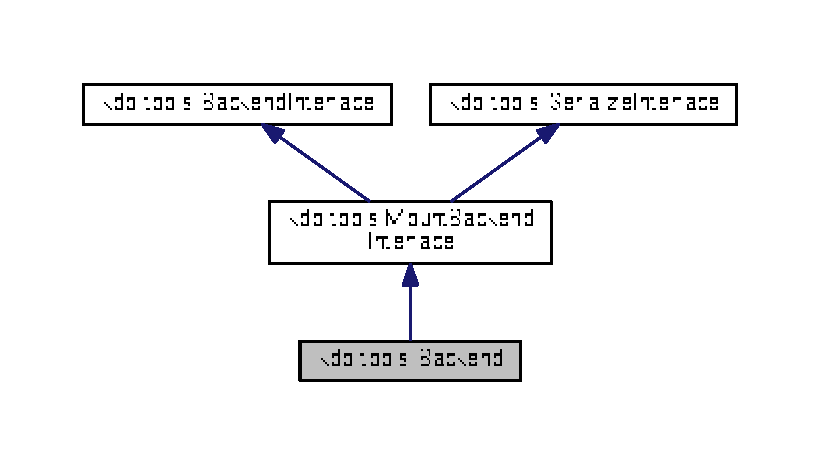
\includegraphics[width=350pt]{classkdb_1_1tools_1_1Backend__inherit__graph}
\end{center}
\end{figure}


Collaboration diagram for kdb\+::tools\+::Backend\+:
\nopagebreak
\begin{figure}[H]
\begin{center}
\leavevmode
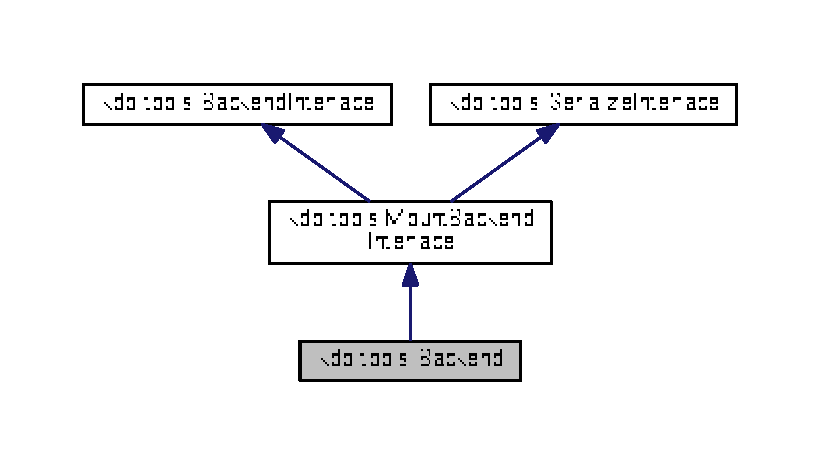
\includegraphics[width=350pt]{classkdb_1_1tools_1_1Backend__coll__graph}
\end{center}
\end{figure}
\doxysubsection*{Public Member Functions}
\begin{DoxyCompactItemize}
\item 
\mbox{\Hypertarget{classkdb_1_1tools_1_1Backend_a1650b149ebf313ee8cd3472247212263}\label{classkdb_1_1tools_1_1Backend_a1650b149ebf313ee8cd3472247212263}} 
\mbox{\hyperlink{classkdb_1_1tools_1_1Backend_a1650b149ebf313ee8cd3472247212263}{Backend}} ()
\begin{DoxyCompactList}\small\item\em Creates a new empty backend. \end{DoxyCompactList}\item 
void \mbox{\hyperlink{classkdb_1_1tools_1_1Backend_ac61b2628800a6fd0a6620ff47bfb3be9}{set\+Mountpoint}} (\mbox{\hyperlink{classkdb_1_1Key}{Key}} mountpoint, \mbox{\hyperlink{classkdb_1_1KeySet}{Key\+Set}} mount\+Conf)
\begin{DoxyCompactList}\small\item\em Sets the mountpoint for the backend. \end{DoxyCompactList}\item 
void \mbox{\hyperlink{classkdb_1_1tools_1_1Backend_aa7aa17a1c97cdfa48bcebadb7bc00247}{set\+Backend\+Config}} (\mbox{\hyperlink{classkdb_1_1KeySet}{Key\+Set}} const \&ks)
\begin{DoxyCompactList}\small\item\em \mbox{\hyperlink{classkdb_1_1tools_1_1Backend}{Backend}} Config to add to. \end{DoxyCompactList}\item 
void \mbox{\hyperlink{classkdb_1_1tools_1_1Backend_a2cce1cc51617baa5431a6036f5cfe05b}{add\+Plugin}} (\mbox{\hyperlink{classkdb_1_1tools_1_1PluginSpec}{Plugin\+Spec}} const \&spec)
\begin{DoxyCompactList}\small\item\em Add a plugin that can be loaded, meets all constraints. \end{DoxyCompactList}\item 
void \mbox{\hyperlink{classkdb_1_1tools_1_1Backend_a5c72747e5419d7802849cfc2eb4064d2}{use\+Config\+File}} (std\+::string file)
\item 
bool \mbox{\hyperlink{classkdb_1_1tools_1_1Backend_a7b28929231bc592c1a83f42121405496}{validated}} () const
\item 
void \mbox{\hyperlink{classkdb_1_1tools_1_1Backend_a93638ae12d8880bdb528ae709c857be7}{serialize}} (\mbox{\hyperlink{classkdb_1_1KeySet}{kdb\+::\+Key\+Set}} \&ret)
\end{DoxyCompactItemize}


\doxysubsection{Detailed Description}
A low-\/level representation of the backend (= set of plugins) that can be mounted. 

To build a backend, you should prefer \mbox{\hyperlink{classkdb_1_1tools_1_1BackendBuilder}{Backend\+Builder}}, which automatically fixes ordering and allows us to remove plugins. 

\doxysubsection{Member Function Documentation}
\mbox{\Hypertarget{classkdb_1_1tools_1_1Backend_a2cce1cc51617baa5431a6036f5cfe05b}\label{classkdb_1_1tools_1_1Backend_a2cce1cc51617baa5431a6036f5cfe05b}} 
\index{kdb::tools::Backend@{kdb::tools::Backend}!addPlugin@{addPlugin}}
\index{addPlugin@{addPlugin}!kdb::tools::Backend@{kdb::tools::Backend}}
\doxysubsubsection{\texorpdfstring{addPlugin()}{addPlugin()}}
{\footnotesize\ttfamily void kdb\+::tools\+::\+Backend\+::add\+Plugin (\begin{DoxyParamCaption}\item[{\mbox{\hyperlink{classkdb_1_1tools_1_1PluginSpec}{Plugin\+Spec}} const \&}]{plugin }\end{DoxyParamCaption})\hspace{0.3cm}{\ttfamily [virtual]}}



Add a plugin that can be loaded, meets all constraints. 

\begin{DoxyNote}{Note}
that this does not mean that the backend validates after it is added. It only means that the situation is not getting worse.
\end{DoxyNote}

\begin{DoxyExceptions}{Exceptions}
{\em Plugin\+Check\+Exception} & or its subclasses if it was not possible to load the plugin\\
\hline
\end{DoxyExceptions}
For validation \begin{DoxySeeAlso}{See also}
\mbox{\hyperlink{classkdb_1_1tools_1_1Backend_a7b28929231bc592c1a83f42121405496}{validated()}}. 
\end{DoxySeeAlso}


Implements \mbox{\hyperlink{classkdb_1_1tools_1_1BackendInterface}{kdb\+::tools\+::\+Backend\+Interface}}.

\mbox{\Hypertarget{classkdb_1_1tools_1_1Backend_a93638ae12d8880bdb528ae709c857be7}\label{classkdb_1_1tools_1_1Backend_a93638ae12d8880bdb528ae709c857be7}} 
\index{kdb::tools::Backend@{kdb::tools::Backend}!serialize@{serialize}}
\index{serialize@{serialize}!kdb::tools::Backend@{kdb::tools::Backend}}
\doxysubsubsection{\texorpdfstring{serialize()}{serialize()}}
{\footnotesize\ttfamily void kdb\+::tools\+::\+Backend\+::serialize (\begin{DoxyParamCaption}\item[{\mbox{\hyperlink{classkdb_1_1KeySet}{kdb\+::\+Key\+Set}} \&}]{ret }\end{DoxyParamCaption})\hspace{0.3cm}{\ttfamily [virtual]}}

\begin{DoxyPrecond}{Precondition}
name and mountpoint set Add plugin serialization into keyset ret.
\end{DoxyPrecond}
Only can be done once! (see first\+Ref in \mbox{\hyperlink{classkdb_1_1tools_1_1Plugin}{Plugin}}) 

Implements \mbox{\hyperlink{classkdb_1_1tools_1_1SerializeInterface}{kdb\+::tools\+::\+Serialize\+Interface}}.

\mbox{\Hypertarget{classkdb_1_1tools_1_1Backend_aa7aa17a1c97cdfa48bcebadb7bc00247}\label{classkdb_1_1tools_1_1Backend_aa7aa17a1c97cdfa48bcebadb7bc00247}} 
\index{kdb::tools::Backend@{kdb::tools::Backend}!setBackendConfig@{setBackendConfig}}
\index{setBackendConfig@{setBackendConfig}!kdb::tools::Backend@{kdb::tools::Backend}}
\doxysubsubsection{\texorpdfstring{setBackendConfig()}{setBackendConfig()}}
{\footnotesize\ttfamily void kdb\+::tools\+::\+Backend\+::set\+Backend\+Config (\begin{DoxyParamCaption}\item[{\mbox{\hyperlink{classkdb_1_1KeySet}{Key\+Set}} const \&}]{ks }\end{DoxyParamCaption})\hspace{0.3cm}{\ttfamily [virtual]}}



\mbox{\hyperlink{classkdb_1_1tools_1_1Backend}{Backend}} Config to add to. 


\begin{DoxyParams}{Parameters}
{\em ks} & the config to add, should be below system/ \\
\hline
\end{DoxyParams}


Implements \mbox{\hyperlink{classkdb_1_1tools_1_1MountBackendInterface}{kdb\+::tools\+::\+Mount\+Backend\+Interface}}.

\mbox{\Hypertarget{classkdb_1_1tools_1_1Backend_ac61b2628800a6fd0a6620ff47bfb3be9}\label{classkdb_1_1tools_1_1Backend_ac61b2628800a6fd0a6620ff47bfb3be9}} 
\index{kdb::tools::Backend@{kdb::tools::Backend}!setMountpoint@{setMountpoint}}
\index{setMountpoint@{setMountpoint}!kdb::tools::Backend@{kdb::tools::Backend}}
\doxysubsubsection{\texorpdfstring{setMountpoint()}{setMountpoint()}}
{\footnotesize\ttfamily void kdb\+::tools\+::\+Backend\+::set\+Mountpoint (\begin{DoxyParamCaption}\item[{\mbox{\hyperlink{classkdb_1_1Key}{Key}}}]{mountpoint,  }\item[{\mbox{\hyperlink{classkdb_1_1KeySet}{Key\+Set}}}]{mount\+Conf }\end{DoxyParamCaption})\hspace{0.3cm}{\ttfamily [virtual]}}



Sets the mountpoint for the backend. 


\begin{DoxyExceptions}{Exceptions}
{\em Mountpoint\+Invalid\+Exception} & \\
\hline
{\em Mountpoint\+Already\+In\+Use\+Exception} & \\
\hline
\end{DoxyExceptions}

\begin{DoxyParams}{Parameters}
{\em mountpoint} & the key name will be used as mountpoint. It is allowed to pass a key with a K\+E\+Y\+\_\+\+C\+A\+S\+C\+A\+D\+I\+N\+G\+\_\+\+N\+A\+ME\\
\hline
{\em mount\+Conf} & needs to include the keys below system/elektra/mountpoints \\
\hline
\end{DoxyParams}


Implements \mbox{\hyperlink{classkdb_1_1tools_1_1MountBackendInterface}{kdb\+::tools\+::\+Mount\+Backend\+Interface}}.

\mbox{\Hypertarget{classkdb_1_1tools_1_1Backend_a5c72747e5419d7802849cfc2eb4064d2}\label{classkdb_1_1tools_1_1Backend_a5c72747e5419d7802849cfc2eb4064d2}} 
\index{kdb::tools::Backend@{kdb::tools::Backend}!useConfigFile@{useConfigFile}}
\index{useConfigFile@{useConfigFile}!kdb::tools::Backend@{kdb::tools::Backend}}
\doxysubsubsection{\texorpdfstring{useConfigFile()}{useConfigFile()}}
{\footnotesize\ttfamily void kdb\+::tools\+::\+Backend\+::use\+Config\+File (\begin{DoxyParamCaption}\item[{std\+::string}]{file }\end{DoxyParamCaption})\hspace{0.3cm}{\ttfamily [virtual]}}

\begin{DoxyPrecond}{Precondition}
\+: resolver needs to be loaded first Will check the filename and use it as config\+File for this backend. 
\end{DoxyPrecond}

\begin{DoxyExceptions}{Exceptions}
{\em File\+Not\+Valid\+Exception} & if filename is not valid \\
\hline
{\em Missing\+Symbol} & if plugin does not implement \textquotesingle{}checkfile\textquotesingle{} \\
\hline
\end{DoxyExceptions}


Implements \mbox{\hyperlink{classkdb_1_1tools_1_1MountBackendInterface}{kdb\+::tools\+::\+Mount\+Backend\+Interface}}.

\mbox{\Hypertarget{classkdb_1_1tools_1_1Backend_a7b28929231bc592c1a83f42121405496}\label{classkdb_1_1tools_1_1Backend_a7b28929231bc592c1a83f42121405496}} 
\index{kdb::tools::Backend@{kdb::tools::Backend}!validated@{validated}}
\index{validated@{validated}!kdb::tools::Backend@{kdb::tools::Backend}}
\doxysubsubsection{\texorpdfstring{validated()}{validated()}}
{\footnotesize\ttfamily bool kdb\+::tools\+::\+Backend\+::validated (\begin{DoxyParamCaption}{ }\end{DoxyParamCaption}) const\hspace{0.3cm}{\ttfamily [virtual]}}

\begin{DoxyReturn}{Returns}
true if backend is validated 

false if more plugins are needed to be valided 
\end{DoxyReturn}


Implements \mbox{\hyperlink{classkdb_1_1tools_1_1MountBackendInterface}{kdb\+::tools\+::\+Mount\+Backend\+Interface}}.



The documentation for this class was generated from the following files\+:\begin{DoxyCompactItemize}
\item 
\mbox{\hyperlink{backend_8hpp}{backend.\+hpp}}\item 
\mbox{\hyperlink{src_2backend_8cpp}{src/backend.\+cpp}}\end{DoxyCompactItemize}

\hypertarget{classkdb_1_1tools_1_1BackendBuilder}{}\section{kdb\+:\+:tools\+:\+:Backend\+Builder Class Reference}
\label{classkdb_1_1tools_1_1BackendBuilder}\index{kdb\+::tools\+::\+Backend\+Builder@{kdb\+::tools\+::\+Backend\+Builder}}


Highlevel interface to build a backend.  




{\ttfamily \#include $<$backendbuilder.\+hpp$>$}



Inheritance diagram for kdb\+:\+:tools\+:\+:Backend\+Builder\+:
\nopagebreak
\begin{figure}[H]
\begin{center}
\leavevmode
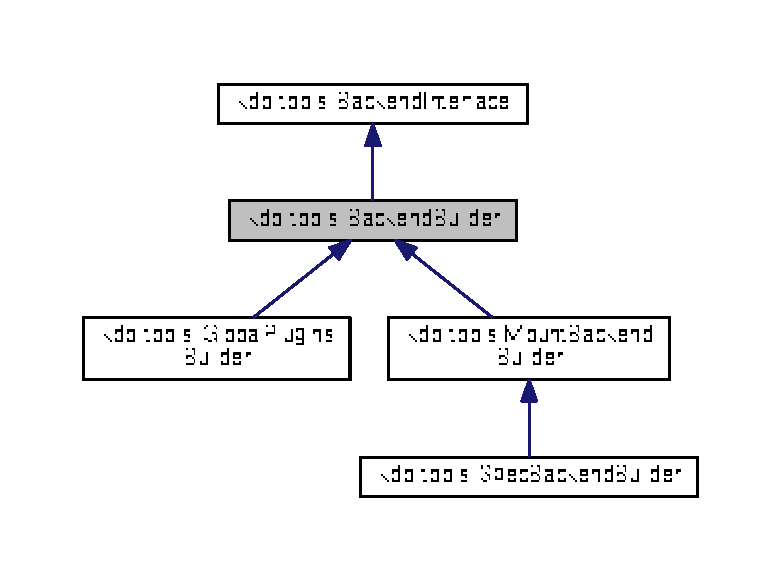
\includegraphics[width=350pt]{classkdb_1_1tools_1_1BackendBuilder__inherit__graph}
\end{center}
\end{figure}


Collaboration diagram for kdb\+:\+:tools\+:\+:Backend\+Builder\+:
\nopagebreak
\begin{figure}[H]
\begin{center}
\leavevmode
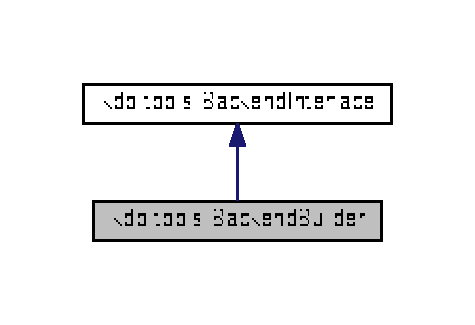
\includegraphics[width=320pt]{classkdb_1_1tools_1_1BackendBuilder__coll__graph}
\end{center}
\end{figure}
\subsection*{Public Member Functions}
\begin{DoxyCompactItemize}
\item 
void \hyperlink{classkdb_1_1tools_1_1BackendBuilder_a987d2c3711399e24b42c38e652c0e1c4}{add\+Plugin} (\hyperlink{classkdb_1_1tools_1_1PluginSpec}{Plugin\+Spec} const \&plugin)
\begin{DoxyCompactList}\small\item\em Add a plugin. \end{DoxyCompactList}\item 
std\+::vector$<$ std\+::string $>$ \hyperlink{classkdb_1_1tools_1_1BackendBuilder_a6e6c23716dc72ef68f8acfd71fc802a9}{resolve\+Needs} (bool add\+Recommends=true)
\begin{DoxyCompactList}\small\item\em resolve all needs that were not resolved by adding plugins. \end{DoxyCompactList}\end{DoxyCompactItemize}


\subsection{Detailed Description}
Highlevel interface to build a backend. 

Automatically reorders plugins and has different modes which \hyperlink{classkdb_1_1tools_1_1Backend}{Backend} should be built. 

\subsection{Member Function Documentation}
\mbox{\Hypertarget{classkdb_1_1tools_1_1BackendBuilder_a987d2c3711399e24b42c38e652c0e1c4}\label{classkdb_1_1tools_1_1BackendBuilder_a987d2c3711399e24b42c38e652c0e1c4}} 
\index{kdb\+::tools\+::\+Backend\+Builder@{kdb\+::tools\+::\+Backend\+Builder}!add\+Plugin@{add\+Plugin}}
\index{add\+Plugin@{add\+Plugin}!kdb\+::tools\+::\+Backend\+Builder@{kdb\+::tools\+::\+Backend\+Builder}}
\subsubsection{\texorpdfstring{add\+Plugin()}{addPlugin()}}
{\footnotesize\ttfamily void kdb\+::tools\+::\+Backend\+Builder\+::add\+Plugin (\begin{DoxyParamCaption}\item[{\hyperlink{classkdb_1_1tools_1_1PluginSpec}{Plugin\+Spec} const \&}]{plugin }\end{DoxyParamCaption})\hspace{0.3cm}{\ttfamily [virtual]}}



Add a plugin. 

\begin{DoxyPrecond}{Precondition}
Needs to be a unique new name (use refname if you want to add the same module multiple times)
\end{DoxyPrecond}
Will automatically resolve virtual plugins to actual plugins.

Also calls the checkconf function if provided by the plugin. The checkconf function has the following signature\+: int checkconf (\hyperlink{classkdb_1_1Key}{Key} $\ast$ error\+Key, \hyperlink{classkdb_1_1KeySet}{Key\+Set} $\ast$ config) and allows a plugin to verify its configuration at mount time.

\begin{DoxySeeAlso}{See also}
\hyperlink{classkdb_1_1tools_1_1BackendBuilder_a6e6c23716dc72ef68f8acfd71fc802a9}{resolve\+Needs()} 
\end{DoxySeeAlso}

\begin{DoxyParams}{Parameters}
{\em plugin} & \\
\hline
\end{DoxyParams}


Implements \hyperlink{classkdb_1_1tools_1_1BackendInterface}{kdb\+::tools\+::\+Backend\+Interface}.



Reimplemented in \hyperlink{classkdb_1_1tools_1_1MountBackendBuilder_a2603e75436a49fc66696c1b41b27efb9}{kdb\+::tools\+::\+Mount\+Backend\+Builder}.

\mbox{\Hypertarget{classkdb_1_1tools_1_1BackendBuilder_a6e6c23716dc72ef68f8acfd71fc802a9}\label{classkdb_1_1tools_1_1BackendBuilder_a6e6c23716dc72ef68f8acfd71fc802a9}} 
\index{kdb\+::tools\+::\+Backend\+Builder@{kdb\+::tools\+::\+Backend\+Builder}!resolve\+Needs@{resolve\+Needs}}
\index{resolve\+Needs@{resolve\+Needs}!kdb\+::tools\+::\+Backend\+Builder@{kdb\+::tools\+::\+Backend\+Builder}}
\subsubsection{\texorpdfstring{resolve\+Needs()}{resolveNeeds()}}
{\footnotesize\ttfamily std\+::vector$<$ std\+::string $>$ kdb\+::tools\+::\+Backend\+Builder\+::resolve\+Needs (\begin{DoxyParamCaption}\item[{bool}]{add\+Recommends = {\ttfamily true} }\end{DoxyParamCaption})}



resolve all needs that were not resolved by adding plugins. 

\begin{DoxyWarning}{Warning}
Must only be used once after all plugins/recommends are added.
\end{DoxyWarning}
\begin{DoxyReturn}{Returns}
the missing recommended plugins 
\end{DoxyReturn}

\begin{DoxyRetVals}{Return values}
{\em empty} & if add\+Recommends was false\\
\hline
\end{DoxyRetVals}
\begin{DoxySeeAlso}{See also}
\hyperlink{classkdb_1_1tools_1_1BackendBuilder_a987d2c3711399e24b42c38e652c0e1c4}{add\+Plugin()} 
\end{DoxySeeAlso}


The documentation for this class was generated from the following files\+:\begin{DoxyCompactItemize}
\item 
\hyperlink{backendbuilder_8hpp}{backendbuilder.\+hpp}\item 
\hyperlink{backendbuilder_8cpp}{backendbuilder.\+cpp}\end{DoxyCompactItemize}

\hypertarget{classkdb_1_1tools_1_1BackendBuilderInit}{}\section{kdb\+::tools\+::Backend\+Builder\+Init Class Reference}
\label{classkdb_1_1tools_1_1BackendBuilderInit}\index{kdb::tools::BackendBuilderInit@{kdb::tools::BackendBuilderInit}}


Used as argument of constructor of $\ast$\+Backend\+Builder.  




{\ttfamily \#include $<$backendbuilder.\+hpp$>$}



\subsection{Detailed Description}
Used as argument of constructor of $\ast$\+Backend\+Builder. 

Avoids the implementation of 5 Constructors for each of the $\ast$\+Backend\+Builder. 

The documentation for this class was generated from the following files\+:\begin{DoxyCompactItemize}
\item 
\mbox{\hyperlink{backendbuilder_8hpp}{backendbuilder.\+hpp}}\item 
\mbox{\hyperlink{backendbuilder_8cpp}{backendbuilder.\+cpp}}\end{DoxyCompactItemize}

\hypertarget{classkdb_1_1tools_1_1BackendFactory}{}\section{kdb\+:\+:tools\+:\+:Backend\+Factory Class Reference}
\label{classkdb_1_1tools_1_1BackendFactory}\index{kdb\+::tools\+::\+Backend\+Factory@{kdb\+::tools\+::\+Backend\+Factory}}


Factory for \hyperlink{classkdb_1_1tools_1_1MountBackendInterface}{Mount\+Backend\+Interface}.  




{\ttfamily \#include $<$backend.\+hpp$>$}

\subsection*{Public Member Functions}
\begin{DoxyCompactItemize}
\item 
\mbox{\Hypertarget{classkdb_1_1tools_1_1BackendFactory_a0e1aadf0f5236a09b623b26dd6085de6}\label{classkdb_1_1tools_1_1BackendFactory_a0e1aadf0f5236a09b623b26dd6085de6}} 
Mount\+Backend\+Interface\+Ptr \hyperlink{classkdb_1_1tools_1_1BackendFactory_a0e1aadf0f5236a09b623b26dd6085de6}{create} () const
\begin{DoxyCompactList}\small\item\em Create classes that implement \hyperlink{classkdb_1_1tools_1_1MountBackendInterface}{Mount\+Backend\+Interface}. \end{DoxyCompactList}\end{DoxyCompactItemize}


\subsection{Detailed Description}
Factory for \hyperlink{classkdb_1_1tools_1_1MountBackendInterface}{Mount\+Backend\+Interface}. 

The documentation for this class was generated from the following file\+:\begin{DoxyCompactItemize}
\item 
\hyperlink{backend_8hpp}{backend.\+hpp}\end{DoxyCompactItemize}

\hypertarget{structkdb_1_1tools_1_1BackendInfo}{}\doxysection{kdb\+::tools\+::Backend\+Info Struct Reference}
\label{structkdb_1_1tools_1_1BackendInfo}\index{kdb::tools::BackendInfo@{kdb::tools::BackendInfo}}


Info about a backend.  




{\ttfamily \#include $<$backends.\+hpp$>$}

\doxysubsection*{Public Attributes}
\begin{DoxyCompactItemize}
\item 
\mbox{\Hypertarget{structkdb_1_1tools_1_1BackendInfo_a7da85fc3a4bbb7412b0544aceeb9da75}\label{structkdb_1_1tools_1_1BackendInfo_a7da85fc3a4bbb7412b0544aceeb9da75}} 
std\+::string \mbox{\hyperlink{structkdb_1_1tools_1_1BackendInfo_a7da85fc3a4bbb7412b0544aceeb9da75}{name}}
\begin{DoxyCompactList}\small\item\em escaped mountpoint name (except for old mountpoints) \end{DoxyCompactList}\item 
\mbox{\Hypertarget{structkdb_1_1tools_1_1BackendInfo_a043c4414dc2b41bab37efb3c878f6cb8}\label{structkdb_1_1tools_1_1BackendInfo_a043c4414dc2b41bab37efb3c878f6cb8}} 
std\+::string \mbox{\hyperlink{structkdb_1_1tools_1_1BackendInfo_a043c4414dc2b41bab37efb3c878f6cb8}{mountpoint}}
\begin{DoxyCompactList}\small\item\em where the backend is mounted \end{DoxyCompactList}\item 
\mbox{\Hypertarget{structkdb_1_1tools_1_1BackendInfo_ac1d9984e01a78dba8e01dca0b91cbf30}\label{structkdb_1_1tools_1_1BackendInfo_ac1d9984e01a78dba8e01dca0b91cbf30}} 
std\+::string \mbox{\hyperlink{structkdb_1_1tools_1_1BackendInfo_ac1d9984e01a78dba8e01dca0b91cbf30}{path}}
\begin{DoxyCompactList}\small\item\em the configuration file path to this backend \end{DoxyCompactList}\end{DoxyCompactItemize}


\doxysubsection{Detailed Description}
Info about a backend. 

The documentation for this struct was generated from the following file\+:\begin{DoxyCompactItemize}
\item 
\mbox{\hyperlink{backends_8hpp}{backends.\+hpp}}\end{DoxyCompactItemize}

\hypertarget{classkdb_1_1tools_1_1BackendInterface}{}\doxysection{kdb\+::tools\+::Backend\+Interface Class Reference}
\label{classkdb_1_1tools_1_1BackendInterface}\index{kdb::tools::BackendInterface@{kdb::tools::BackendInterface}}


Minimal interface to add plugins.  




{\ttfamily \#include $<$backend.\+hpp$>$}



Inheritance diagram for kdb\+::tools\+::Backend\+Interface\+:
\nopagebreak
\begin{figure}[H]
\begin{center}
\leavevmode
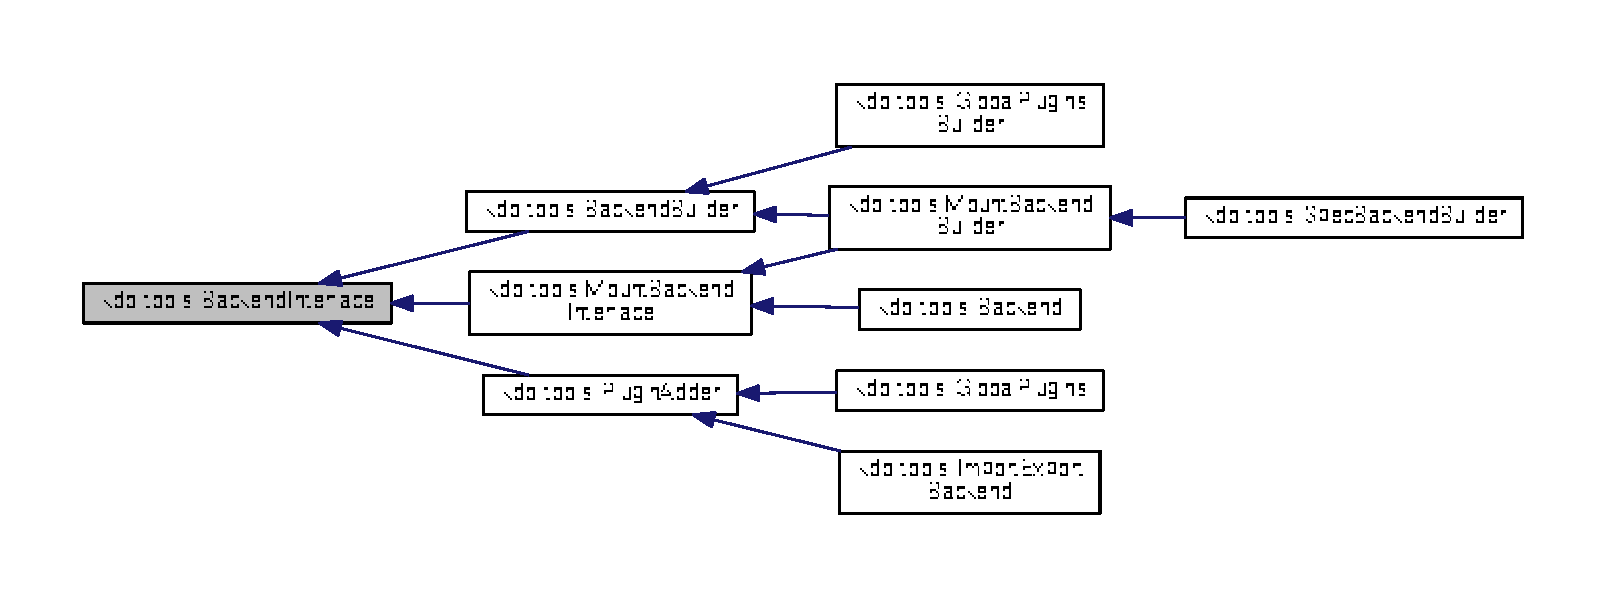
\includegraphics[width=350pt]{classkdb_1_1tools_1_1BackendInterface__inherit__graph}
\end{center}
\end{figure}


\doxysubsection{Detailed Description}
Minimal interface to add plugins. 

The documentation for this class was generated from the following files\+:\begin{DoxyCompactItemize}
\item 
\mbox{\hyperlink{backend_8hpp}{backend.\+hpp}}\item 
\mbox{\hyperlink{src_2backend_8cpp}{src/backend.\+cpp}}\end{DoxyCompactItemize}

\hypertarget{classkdb_1_1tools_1_1Backends}{}\doxysection{kdb\+::tools\+::Backends Class Reference}
\label{classkdb_1_1tools_1_1Backends}\index{kdb::tools::Backends@{kdb::tools::Backends}}


Allows one to list backends.  




{\ttfamily \#include $<$backends.\+hpp$>$}

\doxysubsection*{Static Public Member Functions}
\begin{DoxyCompactItemize}
\item 
static Backend\+Info\+Vector \mbox{\hyperlink{classkdb_1_1tools_1_1Backends_a82b334d8a1e01df664462c6dd43bd7e1}{get\+Backend\+Info}} (\mbox{\hyperlink{classkdb_1_1KeySet}{Key\+Set}} mount\+Conf)
\begin{DoxyCompactList}\small\item\em give info about current mounted backends \end{DoxyCompactList}\item 
static \mbox{\hyperlink{structkdb_1_1tools_1_1BackendInfo}{Backend\+Info}} \mbox{\hyperlink{classkdb_1_1tools_1_1Backends_a692f3f6b5f01ed2e497a6e093e1e2e90}{find\+Backend}} (std\+::string const \&backend, \mbox{\hyperlink{classkdb_1_1KeySet}{Key\+Set}} mount\+Conf, bool verbose=false)
\begin{DoxyCompactList}\small\item\em Find a backend in the given name. \end{DoxyCompactList}\item 
static bool \mbox{\hyperlink{classkdb_1_1tools_1_1Backends_aca36f903059e3df0f2ded569d6d8df8c}{umount}} (std\+::string const \&backend, \mbox{\hyperlink{classkdb_1_1KeySet}{Key\+Set}} \&mount\+Conf)
\begin{DoxyCompactList}\small\item\em Unmount a backend by given mount\+Path. \end{DoxyCompactList}\item 
static std\+::string \mbox{\hyperlink{classkdb_1_1tools_1_1Backends_a76af9122c56426f4d0119e44719c7309}{get\+Base\+Path}} (std\+::string name)
\begin{DoxyCompactList}\small\item\em returns the base path of a mounted backend below system/elektra/mountpoints \end{DoxyCompactList}\end{DoxyCompactItemize}
\doxysubsection*{Static Public Attributes}
\begin{DoxyCompactItemize}
\item 
\mbox{\Hypertarget{classkdb_1_1tools_1_1Backends_ac867850accaab4fda286f763cacc3926}\label{classkdb_1_1tools_1_1Backends_ac867850accaab4fda286f763cacc3926}} 
static const char $\ast$ \mbox{\hyperlink{classkdb_1_1tools_1_1Backends_ac867850accaab4fda286f763cacc3926}{mountpoints\+Path}} = \char`\"{}system/elektra/mountpoints\char`\"{}
\begin{DoxyCompactList}\small\item\em Below this path is the mount\+Conf. \end{DoxyCompactList}\end{DoxyCompactItemize}


\doxysubsection{Detailed Description}
Allows one to list backends. 

\doxysubsection{Member Function Documentation}
\mbox{\Hypertarget{classkdb_1_1tools_1_1Backends_a692f3f6b5f01ed2e497a6e093e1e2e90}\label{classkdb_1_1tools_1_1Backends_a692f3f6b5f01ed2e497a6e093e1e2e90}} 
\index{kdb::tools::Backends@{kdb::tools::Backends}!findBackend@{findBackend}}
\index{findBackend@{findBackend}!kdb::tools::Backends@{kdb::tools::Backends}}
\doxysubsubsection{\texorpdfstring{findBackend()}{findBackend()}}
{\footnotesize\ttfamily \mbox{\hyperlink{structkdb_1_1tools_1_1BackendInfo}{Backend\+Info}} kdb\+::tools\+::\+Backends\+::find\+Backend (\begin{DoxyParamCaption}\item[{std\+::string const \&}]{mount\+Path,  }\item[{\mbox{\hyperlink{classkdb_1_1KeySet}{Key\+Set}}}]{mount\+Conf,  }\item[{bool}]{verbose = {\ttfamily false} }\end{DoxyParamCaption})\hspace{0.3cm}{\ttfamily [static]}}



Find a backend in the given name. 


\begin{DoxyParams}{Parameters}
{\em mount\+Path} & the given backend name to find\\
\hline
\end{DoxyParams}
For backwards compatibility old-\/style names containing \+\_\+ instead of escaped / are accepted if no modern-\/style mountpoint is found.


\begin{DoxyParams}{Parameters}
{\em mount\+Conf} & the configuration to search (should contain keys below mountpoints\+Path to find something)\\
\hline
\end{DoxyParams}
\begin{DoxyReturn}{Returns}
the found backend or an empty \mbox{\hyperlink{structkdb_1_1tools_1_1BackendInfo}{Backend\+Info}} if nothing found (with empty strings) 
\end{DoxyReturn}
\mbox{\Hypertarget{classkdb_1_1tools_1_1Backends_a82b334d8a1e01df664462c6dd43bd7e1}\label{classkdb_1_1tools_1_1Backends_a82b334d8a1e01df664462c6dd43bd7e1}} 
\index{kdb::tools::Backends@{kdb::tools::Backends}!getBackendInfo@{getBackendInfo}}
\index{getBackendInfo@{getBackendInfo}!kdb::tools::Backends@{kdb::tools::Backends}}
\doxysubsubsection{\texorpdfstring{getBackendInfo()}{getBackendInfo()}}
{\footnotesize\ttfamily Backends\+::\+Backend\+Info\+Vector kdb\+::tools\+::\+Backends\+::get\+Backend\+Info (\begin{DoxyParamCaption}\item[{\mbox{\hyperlink{classkdb_1_1KeySet}{Key\+Set}}}]{mount\+Conf }\end{DoxyParamCaption})\hspace{0.3cm}{\ttfamily [static]}}



give info about current mounted backends 


\begin{DoxyParams}{Parameters}
{\em mount\+Conf} & a keyset that contains everything below \mbox{\hyperlink{classkdb_1_1tools_1_1Backends_ac867850accaab4fda286f763cacc3926}{Backends\+::mountpoints\+Path}}\\
\hline
\end{DoxyParams}
\begin{DoxyReturn}{Returns}
an vector of information about mounted backends 
\end{DoxyReturn}
\mbox{\Hypertarget{classkdb_1_1tools_1_1Backends_a76af9122c56426f4d0119e44719c7309}\label{classkdb_1_1tools_1_1Backends_a76af9122c56426f4d0119e44719c7309}} 
\index{kdb::tools::Backends@{kdb::tools::Backends}!getBasePath@{getBasePath}}
\index{getBasePath@{getBasePath}!kdb::tools::Backends@{kdb::tools::Backends}}
\doxysubsubsection{\texorpdfstring{getBasePath()}{getBasePath()}}
{\footnotesize\ttfamily std\+::string kdb\+::tools\+::\+Backends\+::get\+Base\+Path (\begin{DoxyParamCaption}\item[{std\+::string}]{mp }\end{DoxyParamCaption})\hspace{0.3cm}{\ttfamily [static]}}



returns the base path of a mounted backend below system/elektra/mountpoints 


\begin{DoxyParams}{Parameters}
{\em mp} & the mountpoint (name will be derived from it)\\
\hline
\end{DoxyParams}
\begin{DoxyReturn}{Returns}
the properly prefixed and escaped name 
\end{DoxyReturn}
\mbox{\Hypertarget{classkdb_1_1tools_1_1Backends_aca36f903059e3df0f2ded569d6d8df8c}\label{classkdb_1_1tools_1_1Backends_aca36f903059e3df0f2ded569d6d8df8c}} 
\index{kdb::tools::Backends@{kdb::tools::Backends}!umount@{umount}}
\index{umount@{umount}!kdb::tools::Backends@{kdb::tools::Backends}}
\doxysubsubsection{\texorpdfstring{umount()}{umount()}}
{\footnotesize\ttfamily bool kdb\+::tools\+::\+Backends\+::umount (\begin{DoxyParamCaption}\item[{std\+::string const \&}]{mount\+Path,  }\item[{\mbox{\hyperlink{classkdb_1_1KeySet}{Key\+Set}} \&}]{mount\+Conf }\end{DoxyParamCaption})\hspace{0.3cm}{\ttfamily [static]}}



Unmount a backend by given mount\+Path. 


\begin{DoxyParams}{Parameters}
{\em mount\+Path} & the given mountpoint\\
\hline
\end{DoxyParams}
Uses \mbox{\hyperlink{classkdb_1_1tools_1_1Backends_a692f3f6b5f01ed2e497a6e093e1e2e90}{find\+Backend()}} to locate the backend.


\begin{DoxyRetVals}{Return values}
{\em true} & if something was done \\
\hline
{\em false} & if nothing was done (but also no error) \\
\hline
\end{DoxyRetVals}


The documentation for this class was generated from the following files\+:\begin{DoxyCompactItemize}
\item 
\mbox{\hyperlink{backends_8hpp}{backends.\+hpp}}\item 
\mbox{\hyperlink{backends_8cpp}{backends.\+cpp}}\end{DoxyCompactItemize}

\hypertarget{structkdb_1_1Command}{}\section{kdb\+:\+:Command Struct Reference}
\label{structkdb_1_1Command}\index{kdb\+::\+Command@{kdb\+::\+Command}}


Used by contexts for callbacks (to run code using a mutex).  




{\ttfamily \#include $<$kdbvalue.\+hpp$>$}

\subsection*{Public Types}
\begin{DoxyCompactItemize}
\item 
\mbox{\Hypertarget{structkdb_1_1Command_aa49d4f3541e7b5298ae94dfe9c88a67a}\label{structkdb_1_1Command_aa49d4f3541e7b5298ae94dfe9c88a67a}} 
typedef std\+::function$<$ Pair()$>$ \hyperlink{structkdb_1_1Command_aa49d4f3541e7b5298ae94dfe9c88a67a}{Func}
\begin{DoxyCompactList}\small\item\em Typedef for function that returns old\+Key, new\+Key pair. \end{DoxyCompactList}\end{DoxyCompactItemize}


\subsection{Detailed Description}
Used by contexts for callbacks (to run code using a mutex). 

Following scenarios are possible\+: !old\+Name \&\& !new\+Name\+: execute code, do nothing else !old\+Name \&\& new\+Name\+: attach old\+Name \&\& new\+Name\+: reattach old\+Name == new\+Name\+: assignment, attach for inter-\/thread updates old\+Name \&\& !new\+Name\+: detach 

The documentation for this struct was generated from the following file\+:\begin{DoxyCompactItemize}
\item 
\hyperlink{kdbvalue_8hpp}{kdbvalue.\+hpp}\end{DoxyCompactItemize}

\hypertarget{classkdb_1_1Context}{\section{kdb\-:\-:Context Class Reference}
\label{classkdb_1_1Context}\index{kdb\-::\-Context@{kdb\-::\-Context}}
}


Provides a context for configuration.  




{\ttfamily \#include $<$contextual.\-hpp$>$}



Inherits kdb\-::\-Subject.

\subsection*{Public Member Functions}
\begin{DoxyCompactItemize}
\item 
std\-::string \hyperlink{classkdb_1_1Context_a331463d2eec8d2a5fdb8ffe4bfc181f6}{operator\mbox{[}$\,$\mbox{]}} (std\-::string const \&layer) const 
\item 
void \hyperlink{classkdb_1_1Context_aa9ecaf4d6c47dee9ec20d490d09484db}{attach\-By\-Name} (std\-::string const \&key\-\_\-name, Observer \&observer)
\item 
std\-::string \hyperlink{classkdb_1_1Context_a130675fbe20f1b20eaa462ec6a9fe98e}{evaluate} (std\-::string const \&key\-\_\-name) const 
\item 
std\-::string \hyperlink{classkdb_1_1Context_a0687e0df9fbb3e2670fb45f1f9afdfc9}{evaluate} (std\-::string const \&key\-\_\-name, std\-::function$<$ bool(std\-::string const \&, std\-::string \&, bool in\-\_\-group)$>$ const \&on\-\_\-layer) const 
\item 
{\footnotesize template$<$typename T , typename... Args$>$ }\\void \hyperlink{classkdb_1_1Context_a592a5e238bfa36820c561d9dfc0bb8ee}{activate} (Args \&\&...args)
\begin{DoxyCompactList}\small\item\em Globally activate the layer. \end{DoxyCompactList}\end{DoxyCompactItemize}


\subsection{Detailed Description}
Provides a context for configuration. 

Is a subject for observers.

Holds currently active layers and allows global/scoped activation of layers. 

\subsection{Member Function Documentation}
\hypertarget{classkdb_1_1Context_a592a5e238bfa36820c561d9dfc0bb8ee}{\index{kdb\-::\-Context@{kdb\-::\-Context}!activate@{activate}}
\index{activate@{activate}!kdb::Context@{kdb\-::\-Context}}
\subsubsection[{activate}]{\setlength{\rightskip}{0pt plus 5cm}template$<$typename T , typename... Args$>$ void kdb\-::\-Context\-::activate (
\begin{DoxyParamCaption}
\item[{Args \&\&...}]{args}
\end{DoxyParamCaption}
)\hspace{0.3cm}{\ttfamily [inline]}}}\label{classkdb_1_1Context_a592a5e238bfa36820c561d9dfc0bb8ee}


Globally activate the layer. 


\begin{DoxyTemplParams}{Template Parameters}
{\em T} & the layer to activate \\
\hline
{\em Args} & the types for the arguments to pass to layer construction \\
\hline
\end{DoxyTemplParams}

\begin{DoxyParams}{Parameters}
{\em args} & the arguments to pass to layer construction \\
\hline
\end{DoxyParams}
\hypertarget{classkdb_1_1Context_aa9ecaf4d6c47dee9ec20d490d09484db}{\index{kdb\-::\-Context@{kdb\-::\-Context}!attach\-By\-Name@{attach\-By\-Name}}
\index{attach\-By\-Name@{attach\-By\-Name}!kdb::Context@{kdb\-::\-Context}}
\subsubsection[{attach\-By\-Name}]{\setlength{\rightskip}{0pt plus 5cm}void kdb\-::\-Context\-::attach\-By\-Name (
\begin{DoxyParamCaption}
\item[{std\-::string const \&}]{key\-\_\-name, }
\item[{Observer \&}]{observer}
\end{DoxyParamCaption}
)\hspace{0.3cm}{\ttfamily [inline]}}}\label{classkdb_1_1Context_aa9ecaf4d6c47dee9ec20d490d09484db}
Attach observer using to all events given by its specification (name)


\begin{DoxyParams}{Parameters}
{\em key\-\_\-name} & the name with placeholders to be used for attaching \\
\hline
{\em observer} & the observer to attach to \\
\hline
\end{DoxyParams}
\hypertarget{classkdb_1_1Context_a130675fbe20f1b20eaa462ec6a9fe98e}{\index{kdb\-::\-Context@{kdb\-::\-Context}!evaluate@{evaluate}}
\index{evaluate@{evaluate}!kdb::Context@{kdb\-::\-Context}}
\subsubsection[{evaluate}]{\setlength{\rightskip}{0pt plus 5cm}std\-::string kdb\-::\-Context\-::evaluate (
\begin{DoxyParamCaption}
\item[{std\-::string const \&}]{key\-\_\-name}
\end{DoxyParamCaption}
) const\hspace{0.3cm}{\ttfamily [inline]}}}\label{classkdb_1_1Context_a130675fbe20f1b20eaa462ec6a9fe98e}
Evaluate a specification (name) and return a key name under current context


\begin{DoxyParams}{Parameters}
{\em key\-\_\-name} & the name with placeholders to be evaluated \\
\hline
\end{DoxyParams}
\hypertarget{classkdb_1_1Context_a0687e0df9fbb3e2670fb45f1f9afdfc9}{\index{kdb\-::\-Context@{kdb\-::\-Context}!evaluate@{evaluate}}
\index{evaluate@{evaluate}!kdb::Context@{kdb\-::\-Context}}
\subsubsection[{evaluate}]{\setlength{\rightskip}{0pt plus 5cm}std\-::string kdb\-::\-Context\-::evaluate (
\begin{DoxyParamCaption}
\item[{std\-::string const \&}]{key\-\_\-name, }
\item[{std\-::function$<$ bool(std\-::string const \&, std\-::string \&, bool in\-\_\-group)$>$ const \&}]{on\-\_\-layer}
\end{DoxyParamCaption}
) const\hspace{0.3cm}{\ttfamily [inline]}}}\label{classkdb_1_1Context_a0687e0df9fbb3e2670fb45f1f9afdfc9}
Evaluate specification with this context.


\begin{DoxyParams}{Parameters}
{\em key\-\_\-name} & the keyname with placeholders to evaluate \\
\hline
{\em on\-\_\-layer} & the function to be called for every placeholder found\\
\hline
\end{DoxyParams}
\begin{DoxyParagraph}{on\-\_\-layer is called for every layer in the}
specification. 
\end{DoxyParagraph}
\hypertarget{classkdb_1_1Context_a331463d2eec8d2a5fdb8ffe4bfc181f6}{\index{kdb\-::\-Context@{kdb\-::\-Context}!operator\mbox{[}$\,$\mbox{]}@{operator[]}}
\index{operator\mbox{[}$\,$\mbox{]}@{operator[]}!kdb::Context@{kdb\-::\-Context}}
\subsubsection[{operator[]}]{\setlength{\rightskip}{0pt plus 5cm}std\-::string kdb\-::\-Context\-::operator\mbox{[}$\,$\mbox{]} (
\begin{DoxyParamCaption}
\item[{std\-::string const \&}]{layer}
\end{DoxyParamCaption}
) const\hspace{0.3cm}{\ttfamily [inline]}}}\label{classkdb_1_1Context_a331463d2eec8d2a5fdb8ffe4bfc181f6}
Lookup value for a current active layer


\begin{DoxyParams}{Parameters}
{\em layer} & the name of the requested layer \\
\hline
\end{DoxyParams}


The documentation for this class was generated from the following file\-:\begin{DoxyCompactItemize}
\item 
contextual.\-hpp\end{DoxyCompactItemize}

\hypertarget{classkdb_1_1ContextPolicyIs}{}\section{kdb\+::Context\+Policy\+Is$<$ Policy $>$ Class Template Reference}
\label{classkdb_1_1ContextPolicyIs}\index{kdb::ContextPolicyIs$<$ Policy $>$@{kdb::ContextPolicyIs$<$ Policy $>$}}


Needed by the user to set one of the policies.  




{\ttfamily \#include $<$kdbvalue.\+hpp$>$}



Inherits kdb\+::\+Default\+Policies.



\subsection{Detailed Description}
\subsubsection*{template$<$typename Policy$>$\newline
class kdb\+::\+Context\+Policy\+Is$<$ Policy $>$}

Needed by the user to set one of the policies. 


\begin{DoxyTemplParams}{Template Parameters}
{\em Policy} & \\
\hline
\end{DoxyTemplParams}


The documentation for this class was generated from the following file\+:\begin{DoxyCompactItemize}
\item 
\mbox{\hyperlink{kdbvalue_8hpp}{kdbvalue.\+hpp}}\end{DoxyCompactItemize}

\hypertarget{classkdb_1_1Coordinator}{\section{kdb\+:\+:Coordinator Class Reference}
\label{classkdb_1_1Coordinator}\index{kdb\+::\+Coordinator@{kdb\+::\+Coordinator}}
}


Thread safe coordination of Thread\+Context per Threads.  




{\ttfamily \#include $<$kdbthread.\+hpp$>$}



\subsection{Detailed Description}
Thread safe coordination of Thread\+Context per Threads. 

The documentation for this class was generated from the following file\+:\begin{DoxyCompactItemize}
\item 
kdbthread.\+hpp\end{DoxyCompactItemize}

\hypertarget{classkdb_1_1DefaultGetPolicy}{}\section{kdb\+::Default\+Get\+Policy Class Reference}
\label{classkdb_1_1DefaultGetPolicy}\index{kdb::DefaultGetPolicy@{kdb::DefaultGetPolicy}}


Implements lookup with spec.  




{\ttfamily \#include $<$kdbvalue.\+hpp$>$}



\subsection{Detailed Description}
Implements lookup with spec. 

The documentation for this class was generated from the following file\+:\begin{DoxyCompactItemize}
\item 
\mbox{\hyperlink{kdbvalue_8hpp}{kdbvalue.\+hpp}}\end{DoxyCompactItemize}

\hypertarget{classkdb_1_1DefaultSetPolicy}{}\doxysection{kdb\+::Default\+Set\+Policy Class Reference}
\label{classkdb_1_1DefaultSetPolicy}\index{kdb::DefaultSetPolicy@{kdb::DefaultSetPolicy}}


Implements creating user\+:/ key when key is not found.  




{\ttfamily \#include $<$kdbvalue.\+hpp$>$}



\doxysubsection{Detailed Description}
Implements creating user\+:/ key when key is not found. 

The documentation for this class was generated from the following file\+:\begin{DoxyCompactItemize}
\item 
\mbox{\hyperlink{kdbvalue_8hpp}{kdbvalue.\+hpp}}\end{DoxyCompactItemize}

\hypertarget{classkdb_1_1tools_1_1ErrorPlugins}{\section{kdb\+:\+:tools\+:\+:Error\+Plugins Class Reference}
\label{classkdb_1_1tools_1_1ErrorPlugins}\index{kdb\+::tools\+::\+Error\+Plugins@{kdb\+::tools\+::\+Error\+Plugins}}
}


\hyperlink{classkdb_1_1tools_1_1Plugins}{Plugins} to handle errors during configuration access.  




{\ttfamily \#include $<$plugins.\+hpp$>$}



Inheritance diagram for kdb\+:\+:tools\+:\+:Error\+Plugins\+:
\nopagebreak
\begin{figure}[H]
\begin{center}
\leavevmode
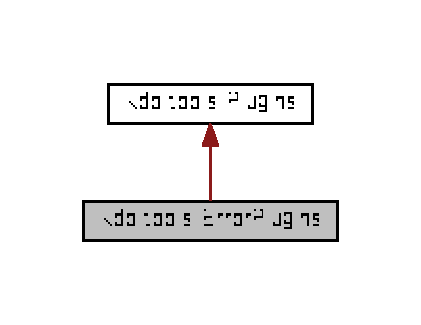
\includegraphics[width=202pt]{classkdb_1_1tools_1_1ErrorPlugins__inherit__graph}
\end{center}
\end{figure}


Collaboration diagram for kdb\+:\+:tools\+:\+:Error\+Plugins\+:
\nopagebreak
\begin{figure}[H]
\begin{center}
\leavevmode
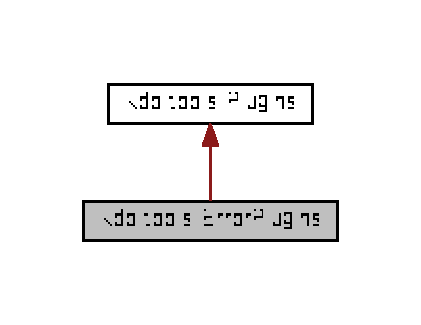
\includegraphics[width=202pt]{classkdb_1_1tools_1_1ErrorPlugins__coll__graph}
\end{center}
\end{figure}


\subsection{Detailed Description}
\hyperlink{classkdb_1_1tools_1_1Plugins}{Plugins} to handle errors during configuration access. 

The documentation for this class was generated from the following files\+:\begin{DoxyCompactItemize}
\item 
\hyperlink{plugins_8hpp}{plugins.\+hpp}\item 
\hyperlink{plugins_8cpp}{plugins.\+cpp}\end{DoxyCompactItemize}

\hypertarget{classkdb_1_1tools_1_1GetPlugins}{\section{kdb\+:\+:tools\+:\+:Get\+Plugins Class Reference}
\label{classkdb_1_1tools_1_1GetPlugins}\index{kdb\+::tools\+::\+Get\+Plugins@{kdb\+::tools\+::\+Get\+Plugins}}
}


\hyperlink{classkdb_1_1tools_1_1Plugins}{Plugins} to get configuration.  




{\ttfamily \#include $<$plugins.\+hpp$>$}



Inheritance diagram for kdb\+:\+:tools\+:\+:Get\+Plugins\+:
\nopagebreak
\begin{figure}[H]
\begin{center}
\leavevmode
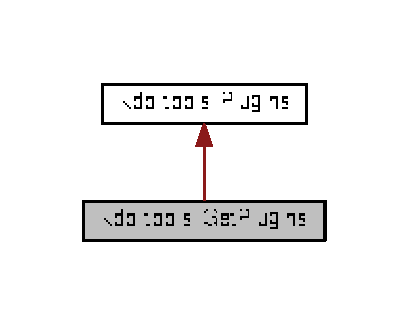
\includegraphics[width=196pt]{classkdb_1_1tools_1_1GetPlugins__inherit__graph}
\end{center}
\end{figure}


Collaboration diagram for kdb\+:\+:tools\+:\+:Get\+Plugins\+:
\nopagebreak
\begin{figure}[H]
\begin{center}
\leavevmode
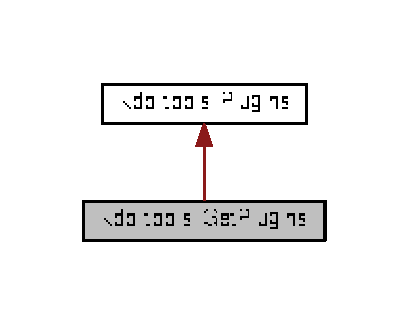
\includegraphics[width=196pt]{classkdb_1_1tools_1_1GetPlugins__coll__graph}
\end{center}
\end{figure}
\subsection*{Public Member Functions}
\begin{DoxyCompactItemize}
\item 
void \hyperlink{classkdb_1_1tools_1_1GetPlugins_a175a3f9bb0054ff13537760fcb0fb861}{try\+Plugin} (\hyperlink{classkdb_1_1tools_1_1Plugin}{Plugin} \&plugin)
\begin{DoxyCompactList}\small\item\em Returns true if \hyperlink{classkdb_1_1tools_1_1GetPlugins}{Get\+Plugins} are valid afterwards. \end{DoxyCompactList}\end{DoxyCompactItemize}


\subsection{Detailed Description}
\hyperlink{classkdb_1_1tools_1_1Plugins}{Plugins} to get configuration. 

\subsection{Member Function Documentation}
\hypertarget{classkdb_1_1tools_1_1GetPlugins_a175a3f9bb0054ff13537760fcb0fb861}{\index{kdb\+::tools\+::\+Get\+Plugins@{kdb\+::tools\+::\+Get\+Plugins}!try\+Plugin@{try\+Plugin}}
\index{try\+Plugin@{try\+Plugin}!kdb\+::tools\+::\+Get\+Plugins@{kdb\+::tools\+::\+Get\+Plugins}}
\subsubsection[{try\+Plugin}]{\setlength{\rightskip}{0pt plus 5cm}void kdb\+::tools\+::\+Get\+Plugins\+::try\+Plugin (
\begin{DoxyParamCaption}
\item[{{\bf Plugin} \&}]{plugin}
\end{DoxyParamCaption}
)}}\label{classkdb_1_1tools_1_1GetPlugins_a175a3f9bb0054ff13537760fcb0fb861}


Returns true if \hyperlink{classkdb_1_1tools_1_1GetPlugins}{Get\+Plugins} are valid afterwards. 

Will throw an exception if plugin could not be added. 

The documentation for this class was generated from the following files\+:\begin{DoxyCompactItemize}
\item 
\hyperlink{plugins_8hpp}{plugins.\+hpp}\item 
\hyperlink{plugins_8cpp}{plugins.\+cpp}\end{DoxyCompactItemize}

\hypertarget{classkdb_1_1GetPolicyIs}{\section{kdb\-:\-:Get\-Policy\-Is$<$ Policy $>$ Class Template Reference}
\label{classkdb_1_1GetPolicyIs}\index{kdb\-::\-Get\-Policy\-Is$<$ Policy $>$@{kdb\-::\-Get\-Policy\-Is$<$ Policy $>$}}
}


Needed by the user to set one of the policies.  




{\ttfamily \#include $<$kdbvalue.\-hpp$>$}



Inherits kdb\-::\-Default\-Policies.



\subsection{Detailed Description}
\subsubsection*{template$<$typename Policy$>$class kdb\-::\-Get\-Policy\-Is$<$ Policy $>$}

Needed by the user to set one of the policies. 


\begin{DoxyTemplParams}{Template Parameters}
{\em Policy} & \\
\hline
\end{DoxyTemplParams}


The documentation for this class was generated from the following file\-:\begin{DoxyCompactItemize}
\item 
kdbvalue.\-hpp\end{DoxyCompactItemize}

\hypertarget{classkdb_1_1tools_1_1GlobalPlugins}{}\section{kdb\+::tools\+::Global\+Plugins Class Reference}
\label{classkdb_1_1tools_1_1GlobalPlugins}\index{kdb::tools::GlobalPlugins@{kdb::tools::GlobalPlugins}}


Low level representation of global plugins.  




{\ttfamily \#include $<$backend.\+hpp$>$}



Inheritance diagram for kdb\+::tools\+::Global\+Plugins\+:
\nopagebreak
\begin{figure}[H]
\begin{center}
\leavevmode
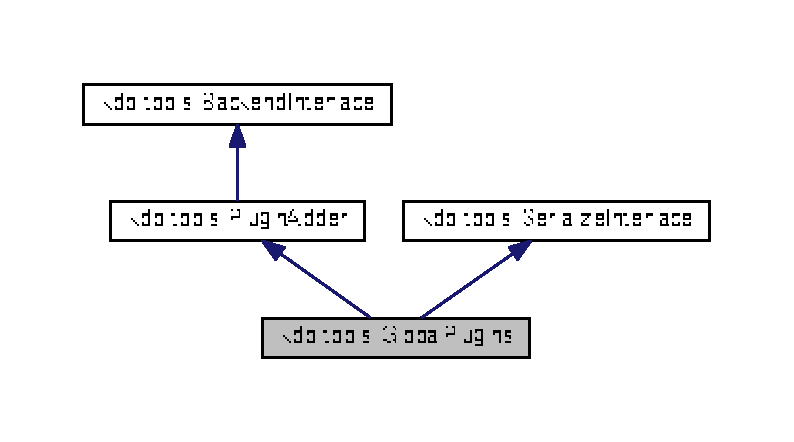
\includegraphics[width=350pt]{classkdb_1_1tools_1_1GlobalPlugins__inherit__graph}
\end{center}
\end{figure}


Collaboration diagram for kdb\+::tools\+::Global\+Plugins\+:
\nopagebreak
\begin{figure}[H]
\begin{center}
\leavevmode
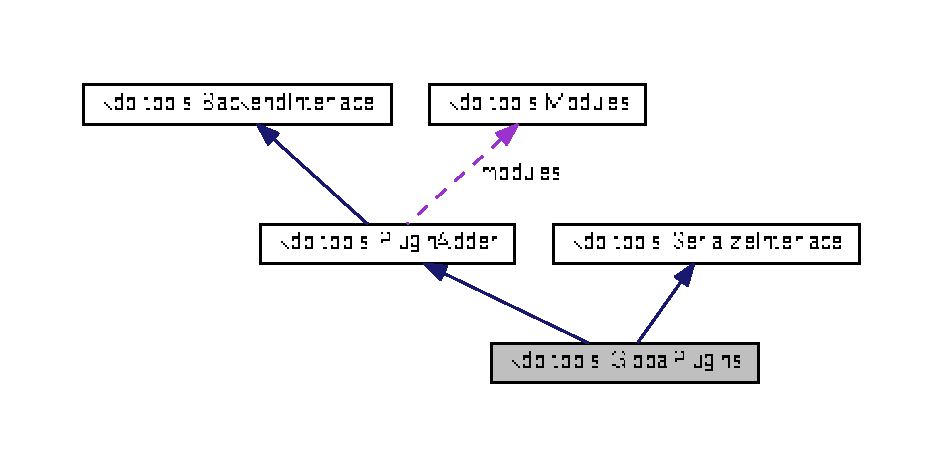
\includegraphics[width=350pt]{classkdb_1_1tools_1_1GlobalPlugins__coll__graph}
\end{center}
\end{figure}


\subsection{Detailed Description}
Low level representation of global plugins. 

The documentation for this class was generated from the following files\+:\begin{DoxyCompactItemize}
\item 
\mbox{\hyperlink{backend_8hpp}{backend.\+hpp}}\item 
\mbox{\hyperlink{src_2backend_8cpp}{src/backend.\+cpp}}\end{DoxyCompactItemize}

\hypertarget{classkdb_1_1tools_1_1GlobalPluginsBuilder}{}\section{kdb\+::tools\+::Global\+Plugins\+Builder Class Reference}
\label{classkdb_1_1tools_1_1GlobalPluginsBuilder}\index{kdb::tools::GlobalPluginsBuilder@{kdb::tools::GlobalPluginsBuilder}}


Build global plugins.  




{\ttfamily \#include $<$backendbuilder.\+hpp$>$}



Inheritance diagram for kdb\+::tools\+::Global\+Plugins\+Builder\+:
\nopagebreak
\begin{figure}[H]
\begin{center}
\leavevmode
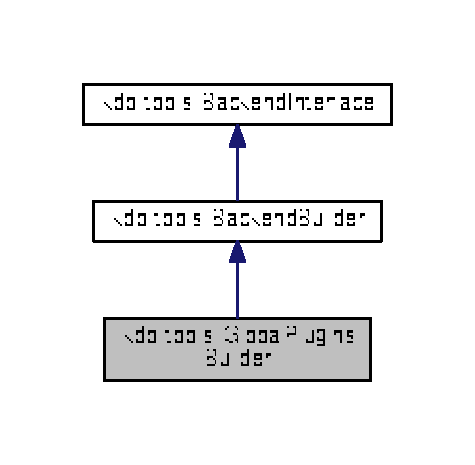
\includegraphics[width=235pt]{classkdb_1_1tools_1_1GlobalPluginsBuilder__inherit__graph}
\end{center}
\end{figure}


Collaboration diagram for kdb\+::tools\+::Global\+Plugins\+Builder\+:
\nopagebreak
\begin{figure}[H]
\begin{center}
\leavevmode
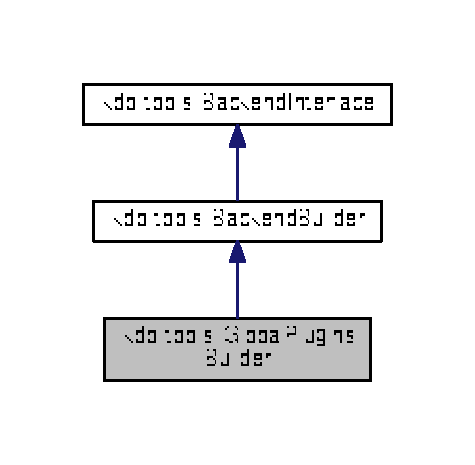
\includegraphics[width=328pt]{classkdb_1_1tools_1_1GlobalPluginsBuilder__coll__graph}
\end{center}
\end{figure}
\subsection*{Static Public Attributes}
\begin{DoxyCompactItemize}
\item 
\mbox{\Hypertarget{classkdb_1_1tools_1_1GlobalPluginsBuilder_ac4300427e2f9e072378f350c0e112156}\label{classkdb_1_1tools_1_1GlobalPluginsBuilder_ac4300427e2f9e072378f350c0e112156}} 
static const char $\ast$ \mbox{\hyperlink{classkdb_1_1tools_1_1GlobalPluginsBuilder_ac4300427e2f9e072378f350c0e112156}{global\+Plugins\+Path}} = \char`\"{}system/elektra/globalplugins\char`\"{}
\begin{DoxyCompactList}\small\item\em Below this path is the configuration for global plugins. \end{DoxyCompactList}\end{DoxyCompactItemize}
\subsection*{Additional Inherited Members}


\subsection{Detailed Description}
Build global plugins. 

The documentation for this class was generated from the following files\+:\begin{DoxyCompactItemize}
\item 
\mbox{\hyperlink{backendbuilder_8hpp}{backendbuilder.\+hpp}}\item 
\mbox{\hyperlink{backendbuilder_8cpp}{backendbuilder.\+cpp}}\end{DoxyCompactItemize}

\hypertarget{structstd_1_1hash_3_01kdb_1_1Key_01_4}{}\section{std\+:\+:hash$<$ kdb\+:\+:Key $>$ Struct Template Reference}
\label{structstd_1_1hash_3_01kdb_1_1Key_01_4}\index{std\+::hash$<$ kdb\+::\+Key $>$@{std\+::hash$<$ kdb\+::\+Key $>$}}


Support for putting Key in a hash.  




{\ttfamily \#include $<$key.\+hpp$>$}



\subsection{Detailed Description}
\subsubsection*{template$<$$>$\newline
struct std\+::hash$<$ kdb\+::\+Key $>$}

Support for putting Key in a hash. 

The documentation for this struct was generated from the following file\+:\begin{DoxyCompactItemize}
\item 
\hyperlink{key_8hpp}{key.\+hpp}\end{DoxyCompactItemize}

\hypertarget{classkdb_1_1tools_1_1ImportExportBackend}{}\section{kdb\+::tools\+::Import\+Export\+Backend Class Reference}
\label{classkdb_1_1tools_1_1ImportExportBackend}\index{kdb::tools::ImportExportBackend@{kdb::tools::ImportExportBackend}}


\mbox{\hyperlink{classkdb_1_1tools_1_1Backend}{Backend}} for import/export functionality.  




{\ttfamily \#include $<$backend.\+hpp$>$}



Inheritance diagram for kdb\+::tools\+::Import\+Export\+Backend\+:
\nopagebreak
\begin{figure}[H]
\begin{center}
\leavevmode
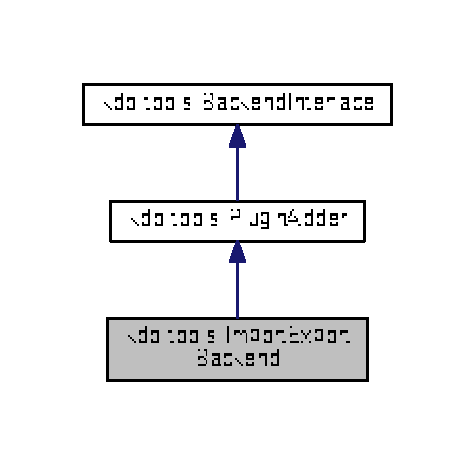
\includegraphics[width=235pt]{classkdb_1_1tools_1_1ImportExportBackend__inherit__graph}
\end{center}
\end{figure}


Collaboration diagram for kdb\+::tools\+::Import\+Export\+Backend\+:
\nopagebreak
\begin{figure}[H]
\begin{center}
\leavevmode
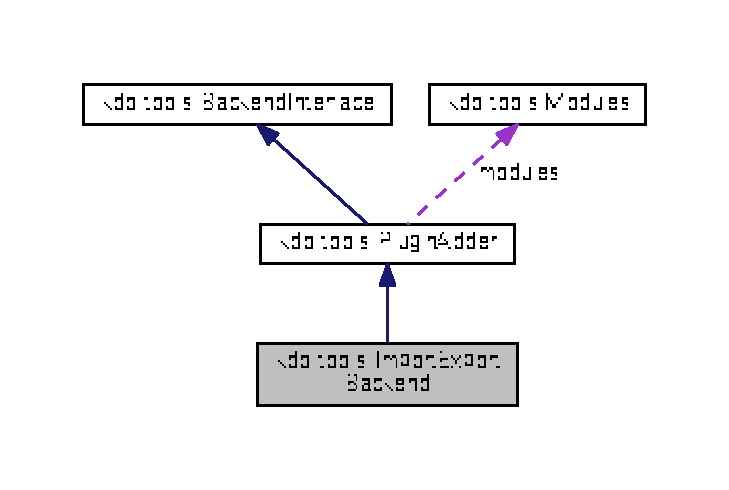
\includegraphics[width=350pt]{classkdb_1_1tools_1_1ImportExportBackend__coll__graph}
\end{center}
\end{figure}


\subsection{Detailed Description}
\mbox{\hyperlink{classkdb_1_1tools_1_1Backend}{Backend}} for import/export functionality. 

(only partly implemented) 

The documentation for this class was generated from the following files\+:\begin{DoxyCompactItemize}
\item 
\mbox{\hyperlink{backend_8hpp}{backend.\+hpp}}\item 
\mbox{\hyperlink{src_2backend_8cpp}{src/backend.\+cpp}}\end{DoxyCompactItemize}

\hypertarget{classkdb_1_1KDB}{}\doxysection{kdb\+::KDB Class Reference}
\label{classkdb_1_1KDB}\index{kdb::KDB@{kdb::KDB}}


Constructs a class \mbox{\hyperlink{classkdb_1_1KDB}{KDB}}.  




{\ttfamily \#include $<$kdb.\+hpp$>$}



Inheritance diagram for kdb\+::KDB\+:
\nopagebreak
\begin{figure}[H]
\begin{center}
\leavevmode
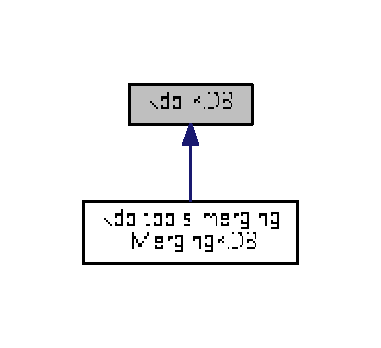
\includegraphics[width=191pt]{classkdb_1_1KDB__inherit__graph}
\end{center}
\end{figure}
\doxysubsection*{Public Member Functions}
\begin{DoxyCompactItemize}
\item 
\mbox{\hyperlink{classkdb_1_1KDB_a7e0637995ce9f294cdbc6f167df6db40}{KDB}} ()
\begin{DoxyCompactList}\small\item\em Constructs a class \mbox{\hyperlink{classkdb_1_1KDB}{KDB}}. \end{DoxyCompactList}\item 
\mbox{\hyperlink{classkdb_1_1KDB_a98e25c7fe2f47c5a90461676c6d219e7}{KDB}} (\mbox{\hyperlink{classkdb_1_1Key}{Key}} \&error\+Key)
\begin{DoxyCompactList}\small\item\em Constructs a class \mbox{\hyperlink{classkdb_1_1KDB}{KDB}}. \end{DoxyCompactList}\item 
\mbox{\hyperlink{classkdb_1_1KDB_adecb001cb936bd869ef06c7c71fdf0ef}{KDB}} (\mbox{\hyperlink{classkdb_1_1KeySet}{Key\+Set}} \&contract)
\begin{DoxyCompactList}\small\item\em Constructs a class \mbox{\hyperlink{classkdb_1_1KDB}{KDB}}. \end{DoxyCompactList}\item 
\mbox{\hyperlink{classkdb_1_1KDB_a95ef4570ac2d7ddbe2b4c0ad7810c742}{KDB}} (\mbox{\hyperlink{classkdb_1_1KeySet}{Key\+Set}} \&contract, \mbox{\hyperlink{classkdb_1_1Key}{Key}} \&error\+Key)
\begin{DoxyCompactList}\small\item\em Constructs a class \mbox{\hyperlink{classkdb_1_1KDB}{KDB}}. \end{DoxyCompactList}\item 
virtual void \mbox{\hyperlink{classkdb_1_1KDB_aee37484b06164eacc0cc11b7b40ab892}{open}} (\mbox{\hyperlink{classkdb_1_1Key}{Key}} \&error\+Key)
\begin{DoxyCompactList}\small\item\em Open the database. \end{DoxyCompactList}\item 
virtual void \mbox{\hyperlink{classkdb_1_1KDB_a8bd17da51bd531a2726185e7bbf4ecf9}{open}} (\mbox{\hyperlink{classkdb_1_1KeySet}{Key\+Set}} \&contract, \mbox{\hyperlink{classkdb_1_1Key}{Key}} \&error\+Key)
\begin{DoxyCompactList}\small\item\em Open the database. \end{DoxyCompactList}\item 
virtual void \mbox{\hyperlink{classkdb_1_1KDB_a1b3ff4a68c2c935d67dce843bc4ad01b}{close}} ()  throw ()
\begin{DoxyCompactList}\small\item\em Close the database. \end{DoxyCompactList}\item 
virtual void \mbox{\hyperlink{classkdb_1_1KDB_aa027a8f798a2cfee11ff712eb204c35d}{close}} (\mbox{\hyperlink{classkdb_1_1Key}{Key}} \&error\+Key)  throw ()
\begin{DoxyCompactList}\small\item\em Close the database. \end{DoxyCompactList}\item 
virtual int \mbox{\hyperlink{classkdb_1_1KDB_a0419ffbc273c89756bc523b4223ec25a}{get}} (\mbox{\hyperlink{classkdb_1_1KeySet}{Key\+Set}} \&returned, std\+::string const \&keyname)
\begin{DoxyCompactList}\small\item\em Get all keys below keyname inside returned. \end{DoxyCompactList}\item 
virtual int \mbox{\hyperlink{classkdb_1_1KDB_a48770a7290699bf2b7529f3ab67e378f}{get}} (\mbox{\hyperlink{classkdb_1_1KeySet}{Key\+Set}} \&returned, \mbox{\hyperlink{classkdb_1_1Key}{Key}} \&parent\+Key)
\begin{DoxyCompactList}\small\item\em Get all keys below parent\+Key inside returned. \end{DoxyCompactList}\item 
virtual int \mbox{\hyperlink{classkdb_1_1KDB_a29087a6a1a7de334f4e5b62ffe5d6e6e}{set}} (\mbox{\hyperlink{classkdb_1_1KeySet}{Key\+Set}} \&returned, std\+::string const \&keyname)
\begin{DoxyCompactList}\small\item\em Set all keys below keyname. \end{DoxyCompactList}\item 
virtual int \mbox{\hyperlink{classkdb_1_1KDB_a62a4fafbe21d9519b31a7868aa05f3e3}{set}} (\mbox{\hyperlink{classkdb_1_1KeySet}{Key\+Set}} \&returned, \mbox{\hyperlink{classkdb_1_1Key}{Key}} \&parent\+Key)
\begin{DoxyCompactList}\small\item\em Set all keys below parent\+Key. \end{DoxyCompactList}\end{DoxyCompactItemize}


\doxysubsection{Detailed Description}
Constructs a class \mbox{\hyperlink{classkdb_1_1KDB}{KDB}}. 


\begin{DoxyExceptions}{Exceptions}
{\em KDBException} & if database could not be opened\\
\hline
\end{DoxyExceptions}
Opens the session with the \mbox{\hyperlink{classkdb_1_1Key}{Key}} database. \begin{DoxyPrecond}{Precondition}
error\+Key must be a valid key, e.\+g. created with \mbox{\hyperlink{group__key_gad23c65b44bf48d773759e1f9a4d43b89}{key\+New()}}
\end{DoxyPrecond}
You must always call this method before retrieving or committing any keys to the database. At the end of a program, after using the \mbox{\hyperlink{classkdb_1_1Key}{Key}} database (\mbox{\hyperlink{classkdb_1_1KDB}{KDB}}), you must not forget to call \mbox{\hyperlink{group__kdb_gadb54dc9fda17ee07deb9444df745c96f}{kdb\+Close()}} to free resources.

The method will bootstrap itself in the following way. The first step is to open the default backend. With it {\ttfamily system\+:/elektra/mountpoints} will be loaded and all needed libraries and mountpoints will be determined. Then the global plugins and global keyset data from the {\ttfamily contract} is processed. Finally, the libraries for backends will be loaded and with it the {\ttfamily \mbox{\hyperlink{classkdb_1_1KDB}{KDB}}} data structure will be initialized.

The pointer to the {\ttfamily \mbox{\hyperlink{classkdb_1_1KDB}{KDB}}} structure returned will be initialized like described above, and it must be passed along on any kdb$\ast$() method your application calls.

Get a {\ttfamily \mbox{\hyperlink{classkdb_1_1KDB}{KDB}}} handle for every thread using elektra. Don\textquotesingle{}t share the handle across threads, and also not the pointer accessing it\+:


\begin{DoxyCodeInclude}{0}
\DoxyCodeLine{\textcolor{keywordtype}{void} thread1 (\textcolor{keywordtype}{void})}
\DoxyCodeLine{\{}
\DoxyCodeLine{        Key * parent = \mbox{\hyperlink{group__key_gad23c65b44bf48d773759e1f9a4d43b89}{keyNew}} (\textcolor{stringliteral}{"{}/app/part1"{}}, \mbox{\hyperlink{group__key_gga9b703ca49f48b482def322b77d3e6bc8aa8adb6fcb92dec58fb19410eacfdd403}{KEY\_END}});}
\DoxyCodeLine{        \mbox{\hyperlink{classkdb_1_1KDB_a7e0637995ce9f294cdbc6f167df6db40}{KDB}} * h = \mbox{\hyperlink{group__kdb_ga844e1299a84c3fbf1d3a905c5c893ba5}{kdbOpen}} (NULL, parent);}
\DoxyCodeLine{        \textcolor{comment}{// fetch keys and work with them}}
\DoxyCodeLine{        \mbox{\hyperlink{group__kdb_gadb54dc9fda17ee07deb9444df745c96f}{kdbClose}} (h, parent);}
\DoxyCodeLine{\}}
\DoxyCodeLine{\textcolor{keywordtype}{void} thread2 (\textcolor{keywordtype}{void})}
\DoxyCodeLine{\{}
\DoxyCodeLine{        Key * parent = \mbox{\hyperlink{group__key_gad23c65b44bf48d773759e1f9a4d43b89}{keyNew}} (\textcolor{stringliteral}{"{}/app/part2"{}}, \mbox{\hyperlink{group__key_gga9b703ca49f48b482def322b77d3e6bc8aa8adb6fcb92dec58fb19410eacfdd403}{KEY\_END}});}
\DoxyCodeLine{        \mbox{\hyperlink{classkdb_1_1KDB_a7e0637995ce9f294cdbc6f167df6db40}{KDB}} * h = \mbox{\hyperlink{group__kdb_ga844e1299a84c3fbf1d3a905c5c893ba5}{kdbOpen}} (NULL, parent);}
\DoxyCodeLine{        \textcolor{comment}{// fetch keys and work with them}}
\DoxyCodeLine{        \mbox{\hyperlink{group__kdb_gadb54dc9fda17ee07deb9444df745c96f}{kdbClose}} (h, parent);}
\DoxyCodeLine{\}}

\end{DoxyCodeInclude}
 You don\textquotesingle{}t need \mbox{\hyperlink{group__kdb_ga844e1299a84c3fbf1d3a905c5c893ba5}{kdb\+Open()}} if you only want to manipulate plain in-\/memory \mbox{\hyperlink{classkdb_1_1Key}{Key}} or \mbox{\hyperlink{classkdb_1_1KeySet}{Key\+Set}} objects.

\begin{DoxyPrecond}{Precondition}
error\+Key must be a valid key, e.\+g. created with \mbox{\hyperlink{group__key_gad23c65b44bf48d773759e1f9a4d43b89}{key\+New()}}
\end{DoxyPrecond}

\begin{DoxyParams}{Parameters}
{\em contract} & the contract that should be ensured before opening the \mbox{\hyperlink{classkdb_1_1KDB}{KDB}} all data is copied and the \mbox{\hyperlink{classkdb_1_1KeySet}{Key\+Set}} can safely be used for e.\+g. \mbox{\hyperlink{group__kdb_ga28e385fd9cb7ccfe0b2f1ed2f62453a1}{kdb\+Get()}} later \\
\hline
{\em error\+Key} & the key which holds errors and warnings which were issued\\
\hline
\end{DoxyParams}
\begin{DoxyReturn}{Returns}
handle to the newly created \mbox{\hyperlink{classkdb_1_1KDB}{KDB}} on success 
\end{DoxyReturn}

\begin{DoxyRetVals}{Return values}
{\em NULL} & on failure\\
\hline
\end{DoxyRetVals}
\begin{DoxySince}{Since}
1.\+0.\+0
\end{DoxySince}
\begin{DoxySeeAlso}{See also}
\mbox{\hyperlink{group__kdb_gadb54dc9fda17ee07deb9444df745c96f}{kdb\+Close()}} to \mbox{\hyperlink{classkdb_1_1KDB_a1b3ff4a68c2c935d67dce843bc4ad01b}{close}} the session of a \mbox{\hyperlink{classkdb_1_1Key}{Key}} database opened by \mbox{\hyperlink{group__kdb_ga844e1299a84c3fbf1d3a905c5c893ba5}{kdb\+Open()}}
\end{DoxySeeAlso}
Access to the key database.

\begin{DoxyInvariant}{Invariant}
the object holds a valid connection to the key database or is empty 
\end{DoxyInvariant}


\doxysubsection{Constructor \& Destructor Documentation}
\mbox{\Hypertarget{classkdb_1_1KDB_a7e0637995ce9f294cdbc6f167df6db40}\label{classkdb_1_1KDB_a7e0637995ce9f294cdbc6f167df6db40}} 
\index{kdb::KDB@{kdb::KDB}!KDB@{KDB}}
\index{KDB@{KDB}!kdb::KDB@{kdb::KDB}}
\doxysubsubsection{\texorpdfstring{KDB()}{KDB()}\hspace{0.1cm}{\footnotesize\ttfamily [1/4]}}
{\footnotesize\ttfamily kdb\+::\+KDB\+::\+KDB (\begin{DoxyParamCaption}{ }\end{DoxyParamCaption})\hspace{0.3cm}{\ttfamily [inline]}}



Constructs a class \mbox{\hyperlink{classkdb_1_1KDB}{KDB}}. 


\begin{DoxyExceptions}{Exceptions}
{\em KDBException} & if database could not be opened\\
\hline
\end{DoxyExceptions}
Opens the session with the \mbox{\hyperlink{classkdb_1_1Key}{Key}} database. \begin{DoxyPrecond}{Precondition}
error\+Key must be a valid key, e.\+g. created with \mbox{\hyperlink{group__key_gad23c65b44bf48d773759e1f9a4d43b89}{key\+New()}}
\end{DoxyPrecond}
You must always call this method before retrieving or committing any keys to the database. At the end of a program, after using the \mbox{\hyperlink{classkdb_1_1Key}{Key}} database (\mbox{\hyperlink{classkdb_1_1KDB}{KDB}}), you must not forget to call \mbox{\hyperlink{group__kdb_gadb54dc9fda17ee07deb9444df745c96f}{kdb\+Close()}} to free resources.

The method will bootstrap itself in the following way. The first step is to open the default backend. With it {\ttfamily system\+:/elektra/mountpoints} will be loaded and all needed libraries and mountpoints will be determined. Then the global plugins and global keyset data from the {\ttfamily contract} is processed. Finally, the libraries for backends will be loaded and with it the {\ttfamily \mbox{\hyperlink{classkdb_1_1KDB}{KDB}}} data structure will be initialized.

The pointer to the {\ttfamily \mbox{\hyperlink{classkdb_1_1KDB}{KDB}}} structure returned will be initialized like described above, and it must be passed along on any kdb$\ast$() method your application calls.

Get a {\ttfamily \mbox{\hyperlink{classkdb_1_1KDB}{KDB}}} handle for every thread using elektra. Don\textquotesingle{}t share the handle across threads, and also not the pointer accessing it\+:


\begin{DoxyCodeInclude}{0}
\DoxyCodeLine{\textcolor{keywordtype}{void} thread1 (\textcolor{keywordtype}{void})}
\DoxyCodeLine{\{}
\DoxyCodeLine{        Key * parent = \mbox{\hyperlink{group__key_gad23c65b44bf48d773759e1f9a4d43b89}{keyNew}} (\textcolor{stringliteral}{"{}/app/part1"{}}, \mbox{\hyperlink{group__key_gga9b703ca49f48b482def322b77d3e6bc8aa8adb6fcb92dec58fb19410eacfdd403}{KEY\_END}});}
\DoxyCodeLine{        \mbox{\hyperlink{classkdb_1_1KDB_a7e0637995ce9f294cdbc6f167df6db40}{KDB}} * h = \mbox{\hyperlink{group__kdb_ga844e1299a84c3fbf1d3a905c5c893ba5}{kdbOpen}} (NULL, parent);}
\DoxyCodeLine{        \textcolor{comment}{// fetch keys and work with them}}
\DoxyCodeLine{        \mbox{\hyperlink{group__kdb_gadb54dc9fda17ee07deb9444df745c96f}{kdbClose}} (h, parent);}
\DoxyCodeLine{\}}
\DoxyCodeLine{\textcolor{keywordtype}{void} thread2 (\textcolor{keywordtype}{void})}
\DoxyCodeLine{\{}
\DoxyCodeLine{        Key * parent = \mbox{\hyperlink{group__key_gad23c65b44bf48d773759e1f9a4d43b89}{keyNew}} (\textcolor{stringliteral}{"{}/app/part2"{}}, \mbox{\hyperlink{group__key_gga9b703ca49f48b482def322b77d3e6bc8aa8adb6fcb92dec58fb19410eacfdd403}{KEY\_END}});}
\DoxyCodeLine{        \mbox{\hyperlink{classkdb_1_1KDB_a7e0637995ce9f294cdbc6f167df6db40}{KDB}} * h = \mbox{\hyperlink{group__kdb_ga844e1299a84c3fbf1d3a905c5c893ba5}{kdbOpen}} (NULL, parent);}
\DoxyCodeLine{        \textcolor{comment}{// fetch keys and work with them}}
\DoxyCodeLine{        \mbox{\hyperlink{group__kdb_gadb54dc9fda17ee07deb9444df745c96f}{kdbClose}} (h, parent);}
\DoxyCodeLine{\}}

\end{DoxyCodeInclude}
 You don\textquotesingle{}t need \mbox{\hyperlink{group__kdb_ga844e1299a84c3fbf1d3a905c5c893ba5}{kdb\+Open()}} if you only want to manipulate plain in-\/memory \mbox{\hyperlink{classkdb_1_1Key}{Key}} or \mbox{\hyperlink{classkdb_1_1KeySet}{Key\+Set}} objects.

\begin{DoxyPrecond}{Precondition}
error\+Key must be a valid key, e.\+g. created with \mbox{\hyperlink{group__key_gad23c65b44bf48d773759e1f9a4d43b89}{key\+New()}}
\end{DoxyPrecond}

\begin{DoxyParams}{Parameters}
{\em contract} & the contract that should be ensured before opening the \mbox{\hyperlink{classkdb_1_1KDB}{KDB}} all data is copied and the \mbox{\hyperlink{classkdb_1_1KeySet}{Key\+Set}} can safely be used for e.\+g. \mbox{\hyperlink{group__kdb_ga28e385fd9cb7ccfe0b2f1ed2f62453a1}{kdb\+Get()}} later \\
\hline
{\em error\+Key} & the key which holds errors and warnings which were issued\\
\hline
\end{DoxyParams}
\begin{DoxyReturn}{Returns}
handle to the newly created \mbox{\hyperlink{classkdb_1_1KDB}{KDB}} on success 
\end{DoxyReturn}

\begin{DoxyRetVals}{Return values}
{\em NULL} & on failure\\
\hline
\end{DoxyRetVals}
\begin{DoxySince}{Since}
1.\+0.\+0
\end{DoxySince}
\begin{DoxySeeAlso}{See also}
\mbox{\hyperlink{group__kdb_gadb54dc9fda17ee07deb9444df745c96f}{kdb\+Close()}} to \mbox{\hyperlink{classkdb_1_1KDB_a1b3ff4a68c2c935d67dce843bc4ad01b}{close}} the session of a \mbox{\hyperlink{classkdb_1_1Key}{Key}} database opened by \mbox{\hyperlink{group__kdb_ga844e1299a84c3fbf1d3a905c5c893ba5}{kdb\+Open()}} 
\end{DoxySeeAlso}
\mbox{\Hypertarget{classkdb_1_1KDB_a98e25c7fe2f47c5a90461676c6d219e7}\label{classkdb_1_1KDB_a98e25c7fe2f47c5a90461676c6d219e7}} 
\index{kdb::KDB@{kdb::KDB}!KDB@{KDB}}
\index{KDB@{KDB}!kdb::KDB@{kdb::KDB}}
\doxysubsubsection{\texorpdfstring{KDB()}{KDB()}\hspace{0.1cm}{\footnotesize\ttfamily [2/4]}}
{\footnotesize\ttfamily kdb\+::\+KDB\+::\+KDB (\begin{DoxyParamCaption}\item[{\mbox{\hyperlink{classkdb_1_1Key}{Key}} \&}]{error\+Key }\end{DoxyParamCaption})\hspace{0.3cm}{\ttfamily [inline]}, {\ttfamily [explicit]}}



Constructs a class \mbox{\hyperlink{classkdb_1_1KDB}{KDB}}. 


\begin{DoxyParams}{Parameters}
{\em error\+Key} & is useful if you want to get the warnings in the successful case, when no exception is thrown.\\
\hline
\end{DoxyParams}

\begin{DoxyExceptions}{Exceptions}
{\em KDBException} & if database could not be opened\\
\hline
\end{DoxyExceptions}
Opens the session with the \mbox{\hyperlink{classkdb_1_1Key}{Key}} database. \begin{DoxyPrecond}{Precondition}
error\+Key must be a valid key, e.\+g. created with \mbox{\hyperlink{group__key_gad23c65b44bf48d773759e1f9a4d43b89}{key\+New()}}
\end{DoxyPrecond}
You must always call this method before retrieving or committing any keys to the database. At the end of a program, after using the \mbox{\hyperlink{classkdb_1_1Key}{Key}} database (\mbox{\hyperlink{classkdb_1_1KDB}{KDB}}), you must not forget to call \mbox{\hyperlink{group__kdb_gadb54dc9fda17ee07deb9444df745c96f}{kdb\+Close()}} to free resources.

The method will bootstrap itself in the following way. The first step is to open the default backend. With it {\ttfamily system\+:/elektra/mountpoints} will be loaded and all needed libraries and mountpoints will be determined. Then the global plugins and global keyset data from the {\ttfamily contract} is processed. Finally, the libraries for backends will be loaded and with it the {\ttfamily \mbox{\hyperlink{classkdb_1_1KDB}{KDB}}} data structure will be initialized.

The pointer to the {\ttfamily \mbox{\hyperlink{classkdb_1_1KDB}{KDB}}} structure returned will be initialized like described above, and it must be passed along on any kdb$\ast$() method your application calls.

Get a {\ttfamily \mbox{\hyperlink{classkdb_1_1KDB}{KDB}}} handle for every thread using elektra. Don\textquotesingle{}t share the handle across threads, and also not the pointer accessing it\+:


\begin{DoxyCodeInclude}{0}
\DoxyCodeLine{\textcolor{keywordtype}{void} thread1 (\textcolor{keywordtype}{void})}
\DoxyCodeLine{\{}
\DoxyCodeLine{        Key * parent = \mbox{\hyperlink{group__key_gad23c65b44bf48d773759e1f9a4d43b89}{keyNew}} (\textcolor{stringliteral}{"{}/app/part1"{}}, \mbox{\hyperlink{group__key_gga9b703ca49f48b482def322b77d3e6bc8aa8adb6fcb92dec58fb19410eacfdd403}{KEY\_END}});}
\DoxyCodeLine{        \mbox{\hyperlink{classkdb_1_1KDB_a7e0637995ce9f294cdbc6f167df6db40}{KDB}} * h = \mbox{\hyperlink{group__kdb_ga844e1299a84c3fbf1d3a905c5c893ba5}{kdbOpen}} (NULL, parent);}
\DoxyCodeLine{        \textcolor{comment}{// fetch keys and work with them}}
\DoxyCodeLine{        \mbox{\hyperlink{group__kdb_gadb54dc9fda17ee07deb9444df745c96f}{kdbClose}} (h, parent);}
\DoxyCodeLine{\}}
\DoxyCodeLine{\textcolor{keywordtype}{void} thread2 (\textcolor{keywordtype}{void})}
\DoxyCodeLine{\{}
\DoxyCodeLine{        Key * parent = \mbox{\hyperlink{group__key_gad23c65b44bf48d773759e1f9a4d43b89}{keyNew}} (\textcolor{stringliteral}{"{}/app/part2"{}}, \mbox{\hyperlink{group__key_gga9b703ca49f48b482def322b77d3e6bc8aa8adb6fcb92dec58fb19410eacfdd403}{KEY\_END}});}
\DoxyCodeLine{        \mbox{\hyperlink{classkdb_1_1KDB_a7e0637995ce9f294cdbc6f167df6db40}{KDB}} * h = \mbox{\hyperlink{group__kdb_ga844e1299a84c3fbf1d3a905c5c893ba5}{kdbOpen}} (NULL, parent);}
\DoxyCodeLine{        \textcolor{comment}{// fetch keys and work with them}}
\DoxyCodeLine{        \mbox{\hyperlink{group__kdb_gadb54dc9fda17ee07deb9444df745c96f}{kdbClose}} (h, parent);}
\DoxyCodeLine{\}}

\end{DoxyCodeInclude}
 You don\textquotesingle{}t need \mbox{\hyperlink{group__kdb_ga844e1299a84c3fbf1d3a905c5c893ba5}{kdb\+Open()}} if you only want to manipulate plain in-\/memory \mbox{\hyperlink{classkdb_1_1Key}{Key}} or \mbox{\hyperlink{classkdb_1_1KeySet}{Key\+Set}} objects.

\begin{DoxyPrecond}{Precondition}
error\+Key must be a valid key, e.\+g. created with \mbox{\hyperlink{group__key_gad23c65b44bf48d773759e1f9a4d43b89}{key\+New()}}
\end{DoxyPrecond}

\begin{DoxyParams}{Parameters}
{\em contract} & the contract that should be ensured before opening the \mbox{\hyperlink{classkdb_1_1KDB}{KDB}} all data is copied and the \mbox{\hyperlink{classkdb_1_1KeySet}{Key\+Set}} can safely be used for e.\+g. \mbox{\hyperlink{group__kdb_ga28e385fd9cb7ccfe0b2f1ed2f62453a1}{kdb\+Get()}} later \\
\hline
{\em error\+Key} & the key which holds errors and warnings which were issued\\
\hline
\end{DoxyParams}
\begin{DoxyReturn}{Returns}
handle to the newly created \mbox{\hyperlink{classkdb_1_1KDB}{KDB}} on success 
\end{DoxyReturn}

\begin{DoxyRetVals}{Return values}
{\em NULL} & on failure\\
\hline
\end{DoxyRetVals}
\begin{DoxySince}{Since}
1.\+0.\+0
\end{DoxySince}
\begin{DoxySeeAlso}{See also}
\mbox{\hyperlink{group__kdb_gadb54dc9fda17ee07deb9444df745c96f}{kdb\+Close()}} to \mbox{\hyperlink{classkdb_1_1KDB_a1b3ff4a68c2c935d67dce843bc4ad01b}{close}} the session of a \mbox{\hyperlink{classkdb_1_1Key}{Key}} database opened by \mbox{\hyperlink{group__kdb_ga844e1299a84c3fbf1d3a905c5c893ba5}{kdb\+Open()}} 
\end{DoxySeeAlso}
\mbox{\Hypertarget{classkdb_1_1KDB_adecb001cb936bd869ef06c7c71fdf0ef}\label{classkdb_1_1KDB_adecb001cb936bd869ef06c7c71fdf0ef}} 
\index{kdb::KDB@{kdb::KDB}!KDB@{KDB}}
\index{KDB@{KDB}!kdb::KDB@{kdb::KDB}}
\doxysubsubsection{\texorpdfstring{KDB()}{KDB()}\hspace{0.1cm}{\footnotesize\ttfamily [3/4]}}
{\footnotesize\ttfamily kdb\+::\+KDB\+::\+KDB (\begin{DoxyParamCaption}\item[{\mbox{\hyperlink{classkdb_1_1KeySet}{Key\+Set}} \&}]{contract }\end{DoxyParamCaption})\hspace{0.3cm}{\ttfamily [inline]}, {\ttfamily [explicit]}}



Constructs a class \mbox{\hyperlink{classkdb_1_1KDB}{KDB}}. 


\begin{DoxyParams}{Parameters}
{\em contract} & the contract that should be ensured \\
\hline
{\em error\+Key} & is useful if you want to get the warnings in the successful case, when no exception is thrown.\\
\hline
\end{DoxyParams}

\begin{DoxyExceptions}{Exceptions}
{\em KDBException} & if database could not be opened\\
\hline
\end{DoxyExceptions}
Opens the session with the \mbox{\hyperlink{classkdb_1_1Key}{Key}} database. \begin{DoxyPrecond}{Precondition}
error\+Key must be a valid key, e.\+g. created with \mbox{\hyperlink{group__key_gad23c65b44bf48d773759e1f9a4d43b89}{key\+New()}}
\end{DoxyPrecond}
You must always call this method before retrieving or committing any keys to the database. At the end of a program, after using the \mbox{\hyperlink{classkdb_1_1Key}{Key}} database (\mbox{\hyperlink{classkdb_1_1KDB}{KDB}}), you must not forget to call \mbox{\hyperlink{group__kdb_gadb54dc9fda17ee07deb9444df745c96f}{kdb\+Close()}} to free resources.

The method will bootstrap itself in the following way. The first step is to open the default backend. With it {\ttfamily system\+:/elektra/mountpoints} will be loaded and all needed libraries and mountpoints will be determined. Then the global plugins and global keyset data from the {\ttfamily contract} is processed. Finally, the libraries for backends will be loaded and with it the {\ttfamily \mbox{\hyperlink{classkdb_1_1KDB}{KDB}}} data structure will be initialized.

The pointer to the {\ttfamily \mbox{\hyperlink{classkdb_1_1KDB}{KDB}}} structure returned will be initialized like described above, and it must be passed along on any kdb$\ast$() method your application calls.

Get a {\ttfamily \mbox{\hyperlink{classkdb_1_1KDB}{KDB}}} handle for every thread using elektra. Don\textquotesingle{}t share the handle across threads, and also not the pointer accessing it\+:


\begin{DoxyCodeInclude}{0}
\DoxyCodeLine{\textcolor{keywordtype}{void} thread1 (\textcolor{keywordtype}{void})}
\DoxyCodeLine{\{}
\DoxyCodeLine{        Key * parent = \mbox{\hyperlink{group__key_gad23c65b44bf48d773759e1f9a4d43b89}{keyNew}} (\textcolor{stringliteral}{"{}/app/part1"{}}, \mbox{\hyperlink{group__key_gga9b703ca49f48b482def322b77d3e6bc8aa8adb6fcb92dec58fb19410eacfdd403}{KEY\_END}});}
\DoxyCodeLine{        \mbox{\hyperlink{classkdb_1_1KDB_a7e0637995ce9f294cdbc6f167df6db40}{KDB}} * h = \mbox{\hyperlink{group__kdb_ga844e1299a84c3fbf1d3a905c5c893ba5}{kdbOpen}} (NULL, parent);}
\DoxyCodeLine{        \textcolor{comment}{// fetch keys and work with them}}
\DoxyCodeLine{        \mbox{\hyperlink{group__kdb_gadb54dc9fda17ee07deb9444df745c96f}{kdbClose}} (h, parent);}
\DoxyCodeLine{\}}
\DoxyCodeLine{\textcolor{keywordtype}{void} thread2 (\textcolor{keywordtype}{void})}
\DoxyCodeLine{\{}
\DoxyCodeLine{        Key * parent = \mbox{\hyperlink{group__key_gad23c65b44bf48d773759e1f9a4d43b89}{keyNew}} (\textcolor{stringliteral}{"{}/app/part2"{}}, \mbox{\hyperlink{group__key_gga9b703ca49f48b482def322b77d3e6bc8aa8adb6fcb92dec58fb19410eacfdd403}{KEY\_END}});}
\DoxyCodeLine{        \mbox{\hyperlink{classkdb_1_1KDB_a7e0637995ce9f294cdbc6f167df6db40}{KDB}} * h = \mbox{\hyperlink{group__kdb_ga844e1299a84c3fbf1d3a905c5c893ba5}{kdbOpen}} (NULL, parent);}
\DoxyCodeLine{        \textcolor{comment}{// fetch keys and work with them}}
\DoxyCodeLine{        \mbox{\hyperlink{group__kdb_gadb54dc9fda17ee07deb9444df745c96f}{kdbClose}} (h, parent);}
\DoxyCodeLine{\}}

\end{DoxyCodeInclude}
 You don\textquotesingle{}t need \mbox{\hyperlink{group__kdb_ga844e1299a84c3fbf1d3a905c5c893ba5}{kdb\+Open()}} if you only want to manipulate plain in-\/memory \mbox{\hyperlink{classkdb_1_1Key}{Key}} or \mbox{\hyperlink{classkdb_1_1KeySet}{Key\+Set}} objects.

\begin{DoxyPrecond}{Precondition}
error\+Key must be a valid key, e.\+g. created with \mbox{\hyperlink{group__key_gad23c65b44bf48d773759e1f9a4d43b89}{key\+New()}}
\end{DoxyPrecond}

\begin{DoxyParams}{Parameters}
{\em contract} & the contract that should be ensured before opening the \mbox{\hyperlink{classkdb_1_1KDB}{KDB}} all data is copied and the \mbox{\hyperlink{classkdb_1_1KeySet}{Key\+Set}} can safely be used for e.\+g. \mbox{\hyperlink{group__kdb_ga28e385fd9cb7ccfe0b2f1ed2f62453a1}{kdb\+Get()}} later \\
\hline
{\em error\+Key} & the key which holds errors and warnings which were issued\\
\hline
\end{DoxyParams}
\begin{DoxyReturn}{Returns}
handle to the newly created \mbox{\hyperlink{classkdb_1_1KDB}{KDB}} on success 
\end{DoxyReturn}

\begin{DoxyRetVals}{Return values}
{\em NULL} & on failure\\
\hline
\end{DoxyRetVals}
\begin{DoxySince}{Since}
1.\+0.\+0
\end{DoxySince}
\begin{DoxySeeAlso}{See also}
\mbox{\hyperlink{group__kdb_gadb54dc9fda17ee07deb9444df745c96f}{kdb\+Close()}} to \mbox{\hyperlink{classkdb_1_1KDB_a1b3ff4a68c2c935d67dce843bc4ad01b}{close}} the session of a \mbox{\hyperlink{classkdb_1_1Key}{Key}} database opened by \mbox{\hyperlink{group__kdb_ga844e1299a84c3fbf1d3a905c5c893ba5}{kdb\+Open()}} 
\end{DoxySeeAlso}
\mbox{\Hypertarget{classkdb_1_1KDB_a95ef4570ac2d7ddbe2b4c0ad7810c742}\label{classkdb_1_1KDB_a95ef4570ac2d7ddbe2b4c0ad7810c742}} 
\index{kdb::KDB@{kdb::KDB}!KDB@{KDB}}
\index{KDB@{KDB}!kdb::KDB@{kdb::KDB}}
\doxysubsubsection{\texorpdfstring{KDB()}{KDB()}\hspace{0.1cm}{\footnotesize\ttfamily [4/4]}}
{\footnotesize\ttfamily kdb\+::\+KDB\+::\+KDB (\begin{DoxyParamCaption}\item[{\mbox{\hyperlink{classkdb_1_1KeySet}{Key\+Set}} \&}]{contract,  }\item[{\mbox{\hyperlink{classkdb_1_1Key}{Key}} \&}]{error\+Key }\end{DoxyParamCaption})\hspace{0.3cm}{\ttfamily [inline]}}



Constructs a class \mbox{\hyperlink{classkdb_1_1KDB}{KDB}}. 


\begin{DoxyParams}{Parameters}
{\em contract} & the contract that should be ensured \\
\hline
{\em error\+Key} & is useful if you want to get the warnings in the successful case, when no exception is thrown.\\
\hline
\end{DoxyParams}

\begin{DoxyExceptions}{Exceptions}
{\em KDBException} & if database could not be opened\\
\hline
\end{DoxyExceptions}
Opens the session with the \mbox{\hyperlink{classkdb_1_1Key}{Key}} database. \begin{DoxyPrecond}{Precondition}
error\+Key must be a valid key, e.\+g. created with \mbox{\hyperlink{group__key_gad23c65b44bf48d773759e1f9a4d43b89}{key\+New()}}
\end{DoxyPrecond}
You must always call this method before retrieving or committing any keys to the database. At the end of a program, after using the \mbox{\hyperlink{classkdb_1_1Key}{Key}} database (\mbox{\hyperlink{classkdb_1_1KDB}{KDB}}), you must not forget to call \mbox{\hyperlink{group__kdb_gadb54dc9fda17ee07deb9444df745c96f}{kdb\+Close()}} to free resources.

The method will bootstrap itself in the following way. The first step is to open the default backend. With it {\ttfamily system\+:/elektra/mountpoints} will be loaded and all needed libraries and mountpoints will be determined. Then the global plugins and global keyset data from the {\ttfamily contract} is processed. Finally, the libraries for backends will be loaded and with it the {\ttfamily \mbox{\hyperlink{classkdb_1_1KDB}{KDB}}} data structure will be initialized.

The pointer to the {\ttfamily \mbox{\hyperlink{classkdb_1_1KDB}{KDB}}} structure returned will be initialized like described above, and it must be passed along on any kdb$\ast$() method your application calls.

Get a {\ttfamily \mbox{\hyperlink{classkdb_1_1KDB}{KDB}}} handle for every thread using elektra. Don\textquotesingle{}t share the handle across threads, and also not the pointer accessing it\+:


\begin{DoxyCodeInclude}{0}
\DoxyCodeLine{\textcolor{keywordtype}{void} thread1 (\textcolor{keywordtype}{void})}
\DoxyCodeLine{\{}
\DoxyCodeLine{        Key * parent = \mbox{\hyperlink{group__key_gad23c65b44bf48d773759e1f9a4d43b89}{keyNew}} (\textcolor{stringliteral}{"{}/app/part1"{}}, \mbox{\hyperlink{group__key_gga9b703ca49f48b482def322b77d3e6bc8aa8adb6fcb92dec58fb19410eacfdd403}{KEY\_END}});}
\DoxyCodeLine{        \mbox{\hyperlink{classkdb_1_1KDB_a7e0637995ce9f294cdbc6f167df6db40}{KDB}} * h = \mbox{\hyperlink{group__kdb_ga844e1299a84c3fbf1d3a905c5c893ba5}{kdbOpen}} (NULL, parent);}
\DoxyCodeLine{        \textcolor{comment}{// fetch keys and work with them}}
\DoxyCodeLine{        \mbox{\hyperlink{group__kdb_gadb54dc9fda17ee07deb9444df745c96f}{kdbClose}} (h, parent);}
\DoxyCodeLine{\}}
\DoxyCodeLine{\textcolor{keywordtype}{void} thread2 (\textcolor{keywordtype}{void})}
\DoxyCodeLine{\{}
\DoxyCodeLine{        Key * parent = \mbox{\hyperlink{group__key_gad23c65b44bf48d773759e1f9a4d43b89}{keyNew}} (\textcolor{stringliteral}{"{}/app/part2"{}}, \mbox{\hyperlink{group__key_gga9b703ca49f48b482def322b77d3e6bc8aa8adb6fcb92dec58fb19410eacfdd403}{KEY\_END}});}
\DoxyCodeLine{        \mbox{\hyperlink{classkdb_1_1KDB_a7e0637995ce9f294cdbc6f167df6db40}{KDB}} * h = \mbox{\hyperlink{group__kdb_ga844e1299a84c3fbf1d3a905c5c893ba5}{kdbOpen}} (NULL, parent);}
\DoxyCodeLine{        \textcolor{comment}{// fetch keys and work with them}}
\DoxyCodeLine{        \mbox{\hyperlink{group__kdb_gadb54dc9fda17ee07deb9444df745c96f}{kdbClose}} (h, parent);}
\DoxyCodeLine{\}}

\end{DoxyCodeInclude}
 You don\textquotesingle{}t need \mbox{\hyperlink{group__kdb_ga844e1299a84c3fbf1d3a905c5c893ba5}{kdb\+Open()}} if you only want to manipulate plain in-\/memory \mbox{\hyperlink{classkdb_1_1Key}{Key}} or \mbox{\hyperlink{classkdb_1_1KeySet}{Key\+Set}} objects.

\begin{DoxyPrecond}{Precondition}
error\+Key must be a valid key, e.\+g. created with \mbox{\hyperlink{group__key_gad23c65b44bf48d773759e1f9a4d43b89}{key\+New()}}
\end{DoxyPrecond}

\begin{DoxyParams}{Parameters}
{\em contract} & the contract that should be ensured before opening the \mbox{\hyperlink{classkdb_1_1KDB}{KDB}} all data is copied and the \mbox{\hyperlink{classkdb_1_1KeySet}{Key\+Set}} can safely be used for e.\+g. \mbox{\hyperlink{group__kdb_ga28e385fd9cb7ccfe0b2f1ed2f62453a1}{kdb\+Get()}} later \\
\hline
{\em error\+Key} & the key which holds errors and warnings which were issued\\
\hline
\end{DoxyParams}
\begin{DoxyReturn}{Returns}
handle to the newly created \mbox{\hyperlink{classkdb_1_1KDB}{KDB}} on success 
\end{DoxyReturn}

\begin{DoxyRetVals}{Return values}
{\em NULL} & on failure\\
\hline
\end{DoxyRetVals}
\begin{DoxySince}{Since}
1.\+0.\+0
\end{DoxySince}
\begin{DoxySeeAlso}{See also}
\mbox{\hyperlink{group__kdb_gadb54dc9fda17ee07deb9444df745c96f}{kdb\+Close()}} to \mbox{\hyperlink{classkdb_1_1KDB_a1b3ff4a68c2c935d67dce843bc4ad01b}{close}} the session of a \mbox{\hyperlink{classkdb_1_1Key}{Key}} database opened by \mbox{\hyperlink{group__kdb_ga844e1299a84c3fbf1d3a905c5c893ba5}{kdb\+Open()}} 
\end{DoxySeeAlso}


\doxysubsection{Member Function Documentation}
\mbox{\Hypertarget{classkdb_1_1KDB_a1b3ff4a68c2c935d67dce843bc4ad01b}\label{classkdb_1_1KDB_a1b3ff4a68c2c935d67dce843bc4ad01b}} 
\index{kdb::KDB@{kdb::KDB}!close@{close}}
\index{close@{close}!kdb::KDB@{kdb::KDB}}
\doxysubsubsection{\texorpdfstring{close()}{close()}\hspace{0.1cm}{\footnotesize\ttfamily [1/2]}}
{\footnotesize\ttfamily void kdb\+::\+KDB\+::close (\begin{DoxyParamCaption}{ }\end{DoxyParamCaption}) throw ( ) \hspace{0.3cm}{\ttfamily [inline]}, {\ttfamily [virtual]}}



Close the database. 

The return value does not matter because its only a null pointer check.

Closes the session with the \mbox{\hyperlink{classkdb_1_1Key}{Key}} database. \begin{DoxyPrecond}{Precondition}
The handle must be a valid handle as returned from \mbox{\hyperlink{group__kdb_ga844e1299a84c3fbf1d3a905c5c893ba5}{kdb\+Open()}} 

error\+Key must be a valid key, e.\+g. created with \mbox{\hyperlink{group__key_gad23c65b44bf48d773759e1f9a4d43b89}{key\+New()}}
\end{DoxyPrecond}
This is the counterpart of \mbox{\hyperlink{group__kdb_ga844e1299a84c3fbf1d3a905c5c893ba5}{kdb\+Open()}}.

You must call this method when you are finished working with the \mbox{\hyperlink{classkdb_1_1Key}{Key}} database. You can manipulate \mbox{\hyperlink{classkdb_1_1Key}{Key}} and \mbox{\hyperlink{classkdb_1_1KeySet}{Key\+Set}} objects also after \mbox{\hyperlink{group__kdb_gadb54dc9fda17ee07deb9444df745c96f}{kdb\+Close()}}, but you must not use any kdb$\ast$() call afterwards.

The {\ttfamily handle} parameter will be finalized and all resources associated to it will be freed. After a \mbox{\hyperlink{group__kdb_gadb54dc9fda17ee07deb9444df745c96f}{kdb\+Close()}}, the {\ttfamily handle} cannot be used anymore.


\begin{DoxyParams}{Parameters}
{\em handle} & contains internal information of \mbox{\hyperlink{group__kdb_ga844e1299a84c3fbf1d3a905c5c893ba5}{opened }} key database \\
\hline
{\em error\+Key} & the key which holds error/warning information\\
\hline
\end{DoxyParams}

\begin{DoxyRetVals}{Return values}
{\em 0} & on success \\
\hline
{\em -\/1} & on NULL pointer\\
\hline
\end{DoxyRetVals}
\begin{DoxySince}{Since}
1.\+0.\+0
\end{DoxySince}
\begin{DoxySeeAlso}{See also}
\mbox{\hyperlink{group__kdb_ga844e1299a84c3fbf1d3a905c5c893ba5}{kdb\+Open()}} for opening a session with a \mbox{\hyperlink{classkdb_1_1Key}{Key}} database 
\end{DoxySeeAlso}
\mbox{\Hypertarget{classkdb_1_1KDB_aa027a8f798a2cfee11ff712eb204c35d}\label{classkdb_1_1KDB_aa027a8f798a2cfee11ff712eb204c35d}} 
\index{kdb::KDB@{kdb::KDB}!close@{close}}
\index{close@{close}!kdb::KDB@{kdb::KDB}}
\doxysubsubsection{\texorpdfstring{close()}{close()}\hspace{0.1cm}{\footnotesize\ttfamily [2/2]}}
{\footnotesize\ttfamily void kdb\+::\+KDB\+::close (\begin{DoxyParamCaption}\item[{\mbox{\hyperlink{classkdb_1_1Key}{Key}} \&}]{error\+Key }\end{DoxyParamCaption}) throw ( ) \hspace{0.3cm}{\ttfamily [inline]}, {\ttfamily [virtual]}}



Close the database. 

The return value does not matter because its only a null pointer check.


\begin{DoxyParams}{Parameters}
{\em error\+Key} & is useful if you want to get the warnings\\
\hline
\end{DoxyParams}
Closes the session with the \mbox{\hyperlink{classkdb_1_1Key}{Key}} database. \begin{DoxyPrecond}{Precondition}
The handle must be a valid handle as returned from \mbox{\hyperlink{group__kdb_ga844e1299a84c3fbf1d3a905c5c893ba5}{kdb\+Open()}} 

error\+Key must be a valid key, e.\+g. created with \mbox{\hyperlink{group__key_gad23c65b44bf48d773759e1f9a4d43b89}{key\+New()}}
\end{DoxyPrecond}
This is the counterpart of \mbox{\hyperlink{group__kdb_ga844e1299a84c3fbf1d3a905c5c893ba5}{kdb\+Open()}}.

You must call this method when you are finished working with the \mbox{\hyperlink{classkdb_1_1Key}{Key}} database. You can manipulate \mbox{\hyperlink{classkdb_1_1Key}{Key}} and \mbox{\hyperlink{classkdb_1_1KeySet}{Key\+Set}} objects also after \mbox{\hyperlink{group__kdb_gadb54dc9fda17ee07deb9444df745c96f}{kdb\+Close()}}, but you must not use any kdb$\ast$() call afterwards.

The {\ttfamily handle} parameter will be finalized and all resources associated to it will be freed. After a \mbox{\hyperlink{group__kdb_gadb54dc9fda17ee07deb9444df745c96f}{kdb\+Close()}}, the {\ttfamily handle} cannot be used anymore.


\begin{DoxyParams}{Parameters}
{\em handle} & contains internal information of \mbox{\hyperlink{group__kdb_ga844e1299a84c3fbf1d3a905c5c893ba5}{opened }} key database \\
\hline
{\em error\+Key} & the key which holds error/warning information\\
\hline
\end{DoxyParams}

\begin{DoxyRetVals}{Return values}
{\em 0} & on success \\
\hline
{\em -\/1} & on NULL pointer\\
\hline
\end{DoxyRetVals}
\begin{DoxySince}{Since}
1.\+0.\+0
\end{DoxySince}
\begin{DoxySeeAlso}{See also}
\mbox{\hyperlink{group__kdb_ga844e1299a84c3fbf1d3a905c5c893ba5}{kdb\+Open()}} for opening a session with a \mbox{\hyperlink{classkdb_1_1Key}{Key}} database 
\end{DoxySeeAlso}
\mbox{\Hypertarget{classkdb_1_1KDB_a48770a7290699bf2b7529f3ab67e378f}\label{classkdb_1_1KDB_a48770a7290699bf2b7529f3ab67e378f}} 
\index{kdb::KDB@{kdb::KDB}!get@{get}}
\index{get@{get}!kdb::KDB@{kdb::KDB}}
\doxysubsubsection{\texorpdfstring{get()}{get()}\hspace{0.1cm}{\footnotesize\ttfamily [1/2]}}
{\footnotesize\ttfamily int kdb\+::\+KDB\+::get (\begin{DoxyParamCaption}\item[{\mbox{\hyperlink{classkdb_1_1KeySet}{Key\+Set}} \&}]{returned,  }\item[{\mbox{\hyperlink{classkdb_1_1Key}{Key}} \&}]{parent\+Key }\end{DoxyParamCaption})\hspace{0.3cm}{\ttfamily [inline]}, {\ttfamily [virtual]}}



Get all keys below parent\+Key inside returned. 

Retrieve Keys from the \mbox{\hyperlink{classkdb_1_1Key}{Key}} database in an atomic and universal way. \begin{DoxyPrecond}{Precondition}
The {\ttfamily handle} must be a valid \mbox{\hyperlink{classkdb_1_1KDB}{KDB}} handle as returned from \mbox{\hyperlink{group__kdb_ga844e1299a84c3fbf1d3a905c5c893ba5}{kdb\+Open()}}. 

The \mbox{\hyperlink{classkdb_1_1KeySet}{Key\+Set}} {\ttfamily returned} must be a valid \mbox{\hyperlink{classkdb_1_1KeySet}{Key\+Set}}, i.\+e., constructed with \mbox{\hyperlink{group__keyset_ga671e1aaee3ae9dc13b4834a4ddbd2c3c}{ks\+New()}}. 

The \mbox{\hyperlink{classkdb_1_1KeySet}{Key\+Set}} {\ttfamily returned} must contain keys only from the {\ttfamily spec\+:/}, {\ttfamily dir\+:/}, {\ttfamily user\+:/}, {\ttfamily system\+:/}, {\ttfamily default\+:/} or {\ttfamily proc\+:/} namespaces. 

The \mbox{\hyperlink{classkdb_1_1Key}{Key}} {\ttfamily parent\+Key} must be a valid \mbox{\hyperlink{classkdb_1_1Key}{Key}}, i.\+e., constructed with \mbox{\hyperlink{group__key_gad23c65b44bf48d773759e1f9a4d43b89}{key\+New()}}. 

The \mbox{\hyperlink{classkdb_1_1Key}{Key}} {\ttfamily parent\+Key} must not have read-\/only name, value or metadata. 

The \mbox{\hyperlink{classkdb_1_1Key}{Key}} {\ttfamily parent\+Key} must use the {\ttfamily spec\+:/}, {\ttfamily dir\+:/}, {\ttfamily user\+:/}, {\ttfamily system\+:/}, {\ttfamily default\+:/}, {\ttfamily proc\+:/} or cascading namespace.
\end{DoxyPrecond}
If you pass {\ttfamily NULL} or a key with read-\/only metadata as {\ttfamily parent\+Key}, \mbox{\hyperlink{group__kdb_ga28e385fd9cb7ccfe0b2f1ed2f62453a1}{kdb\+Get()}} will fail immediately without doing anything. If you pass another invalid {\ttfamily parent\+Key}, or {\ttfamily NULL} as {\ttfamily ks} or {\ttfamily handle}, \mbox{\hyperlink{group__kdb_ga28e385fd9cb7ccfe0b2f1ed2f62453a1}{kdb\+Get()}} will set an error on {\ttfamily parent\+Key} and then return immediately.

\begin{DoxyNote}{Note}
If you pass a non-\/\+NULL {\ttfamily parent\+Key} with writable metadata, \mbox{\hyperlink{group__kdb_ga28e385fd9cb7ccfe0b2f1ed2f62453a1}{kdb\+Get()}} will {\bfseries{always}} remove any existing errors and warnings from {\ttfamily parent\+Key}.
\end{DoxyNote}
\begin{DoxyWarning}{Warning}
If you later call \mbox{\hyperlink{group__kdb_ga11436b058408f83d303ca5e996832bcf}{kdb\+Set()}} with the same {\ttfamily handle} you must make sure to pass all keys from {\ttfamily ks}, which you do not want to remove.
\end{DoxyWarning}
\begin{DoxyParagraph}{Loadable Namespaces}

\end{DoxyParagraph}
Not all namespace can be loaded.


\begin{DoxyItemize}
\item {\ttfamily spec\+:/}, {\ttfamily dir\+:/}, {\ttfamily user\+:/} and {\ttfamily system\+:/} can be loaded via \mbox{\hyperlink{group__kdb_ga28e385fd9cb7ccfe0b2f1ed2f62453a1}{kdb\+Get()}}.
\item {\ttfamily proc\+:/} keys can be loaded via \mbox{\hyperlink{group__kdb_ga28e385fd9cb7ccfe0b2f1ed2f62453a1}{kdb\+Get()}}, but are not persisted or cached.
\item {\ttfamily default\+:/} keys can be inserted by \mbox{\hyperlink{group__kdb_ga28e385fd9cb7ccfe0b2f1ed2f62453a1}{kdb\+Get()}} but they will always stem from a specification in {\ttfamily spec\+:/} keys.
\item If {\ttfamily ks} contains a key with any other namespace, an error will be returned.
\end{DoxyItemize}

\begin{DoxyParagraph}{Parent Key}

\end{DoxyParagraph}
The {\ttfamily parent\+Key} defines which parts of {\ttfamily ks} will be loaded. Everything that is at or below {\ttfamily parent\+Key} wil be loaded together with any key that shares a backend with such a key. Backends are always loaded as an atomic unit.

\begin{DoxyNote}{Note}
If {\ttfamily parent\+Key} is in the cascading namespace, keys of all loadable namespaces (see above) will be loaded. This is generally the recommended approach.
\end{DoxyNote}
Upon sucessfully returning \mbox{\hyperlink{group__kdb_ga28e385fd9cb7ccfe0b2f1ed2f62453a1}{kdb\+Get()}} also sets the value of {\ttfamily parent\+Key} to the storage identifier used by the backend that contains (or would contain) {\ttfamily parent\+Key}. For file-\/based backends this is the absolute path of the underlying file. Other backends may use different identifiers, but it always uniquely identifies the underlying storage unit.

\begin{DoxyNote}{Note}
If {\ttfamily parent\+Key} is in the cascading, {\ttfamily default\+:/} or \`{}proc\+:/ namespace, the value of {\ttfamily parent\+Key} will be set to an empty string. This is done, because those namespaces are not persistable (see \mbox{\hyperlink{group__kdb_ga11436b058408f83d303ca5e996832bcf}{kdb\+Set()}}) and therfore have no storage identifier.
\end{DoxyNote}
\begin{DoxyParagraph}{Key\+Set Modifications}

\end{DoxyParagraph}
Below or at {\ttfamily parent\+Key}, the \mbox{\hyperlink{classkdb_1_1KeySet}{Key\+Set}} {\ttfamily ks} will mostly contain keys loaded from backends. The only exception are {\ttfamily proc\+:/} and {\ttfamily spec\+:/} keys that were already present, before \mbox{\hyperlink{group__kdb_ga28e385fd9cb7ccfe0b2f1ed2f62453a1}{kdb\+Get()}} was called and do not overlap with an existing backend (for those namespaces). This can be used to provide a hard-\/coded fallback specifications and/or process-\/specific data.

Keys not below (or at) {\ttfamily parent\+Key} that were present when \mbox{\hyperlink{group__kdb_ga28e385fd9cb7ccfe0b2f1ed2f62453a1}{kdb\+Get()}} was called, may still be removed. For example, this could be because they overlap with a backend that also has keys below {\ttfamily parent\+Key} (backends are atomic units).

\begin{DoxyParagraph}{Example\+:}
This example demonstrates the typical usecase within an application (without error handling).
\end{DoxyParagraph}

\begin{DoxyCodeInclude}{0}
\DoxyCodeLine{}
\DoxyCodeLine{\textcolor{preprocessor}{\#include <kdb.h>}}
\DoxyCodeLine{\textcolor{preprocessor}{\#include <stdio.h>}}
\DoxyCodeLine{}
\DoxyCodeLine{\textcolor{keywordtype}{int} \mbox{\hyperlink{testio__doc_8c_a3c04138a5bfe5d72780bb7e82a18e627}{main}} (\textcolor{keywordtype}{void})}
\DoxyCodeLine{\{}
\DoxyCodeLine{        KeySet * myConfig = \mbox{\hyperlink{group__keyset_ga671e1aaee3ae9dc13b4834a4ddbd2c3c}{ksNew}} (0, \mbox{\hyperlink{group__keyset_ga7a28fce3773b2c873c94ac80b8b4cd54}{KS\_END}});}
\DoxyCodeLine{}
\DoxyCodeLine{        \textcolor{comment}{// for error handling see kdbget\_error.c}}
\DoxyCodeLine{}
\DoxyCodeLine{        \textcolor{comment}{// clang-\/format off}}
\DoxyCodeLine{\textcolor{comment}{}Key * key = \mbox{\hyperlink{group__key_gad23c65b44bf48d773759e1f9a4d43b89}{keyNew}} (\textcolor{stringliteral}{"{}/sw/tests/myapp/\#0/current/"{}},  \mbox{\hyperlink{group__key_gga9b703ca49f48b482def322b77d3e6bc8aa8adb6fcb92dec58fb19410eacfdd403}{KEY\_END}});}
\DoxyCodeLine{\mbox{\hyperlink{classkdb_1_1KDB_a7e0637995ce9f294cdbc6f167df6db40}{KDB}} * handle = \mbox{\hyperlink{group__kdb_ga844e1299a84c3fbf1d3a905c5c893ba5}{kdbOpen}} (NULL, key);}
\DoxyCodeLine{\mbox{\hyperlink{group__kdb_ga28e385fd9cb7ccfe0b2f1ed2f62453a1}{kdbGet}} (handle, myConfig, key);}
\DoxyCodeLine{Key * result = \mbox{\hyperlink{group__keyset_gad65d2cdcbb5381194a1688e169af8a83}{ksLookupByName}} (myConfig, \textcolor{stringliteral}{"{}/sw/tests/myapp/\#0/current/testkey1"{}}, 0);}
\DoxyCodeLine{        \textcolor{comment}{// clang-\/format on}}
\DoxyCodeLine{}
\DoxyCodeLine{        \mbox{\hyperlink{group__key_ga3df95bbc2494e3e6703ece5639be5bb1}{keyDel}} (key);}
\DoxyCodeLine{}
\DoxyCodeLine{        \textcolor{keyword}{const} \textcolor{keywordtype}{char} * key\_name = \mbox{\hyperlink{group__keyname_ga8e805c726a60da921d3736cda7813513}{keyName}} (result);}
\DoxyCodeLine{        \textcolor{keyword}{const} \textcolor{keywordtype}{char} * key\_value = \mbox{\hyperlink{group__keyvalue_ga880936f2481d28e6e2acbe7486a21d05}{keyString}} (result);}
\DoxyCodeLine{        \textcolor{keyword}{const} \textcolor{keywordtype}{char} * key\_comment = \mbox{\hyperlink{group__keyvalue_ga880936f2481d28e6e2acbe7486a21d05}{keyString}} (\mbox{\hyperlink{group__keymeta_ga9ed3875495ddb3d8a8d29158a60a147c}{keyGetMeta}} (result, \textcolor{stringliteral}{"{}comment/\#0"{}}));}
\DoxyCodeLine{        printf (\textcolor{stringliteral}{"{}key: \%s value: \%s comment: \%s\(\backslash\)n"{}}, key\_name, key\_value, key\_comment);}
\DoxyCodeLine{}
\DoxyCodeLine{        \mbox{\hyperlink{group__keyset_ga27e5c16473b02a422238c8d970db7ac8}{ksDel}} (myConfig); \textcolor{comment}{// delete the in-\/memory configuration}}
\DoxyCodeLine{}
\DoxyCodeLine{}
\DoxyCodeLine{        \textcolor{comment}{// maybe you want kdbSet() myConfig here}}
\DoxyCodeLine{}
\DoxyCodeLine{        \mbox{\hyperlink{group__kdb_gadb54dc9fda17ee07deb9444df745c96f}{kdbClose}} (handle, 0); \textcolor{comment}{// no more affairs with the key database.}}
\DoxyCodeLine{\}}

\end{DoxyCodeInclude}


When a backend fails \mbox{\hyperlink{group__kdb_ga28e385fd9cb7ccfe0b2f1ed2f62453a1}{kdb\+Get()}} will return -\/1 with all error and warning information in the {\ttfamily parent\+Key}. The parameter {\ttfamily returned} will not be changed.

\begin{DoxyParagraph}{Optimization\+:}
In the first run of kdb\+Get all requested (or more) Keys are retrieved. On subsequent calls only the Keys are retrieved where something was changed inside the \mbox{\hyperlink{classkdb_1_1Key}{Key}} database. The other Keys stay in the \mbox{\hyperlink{classkdb_1_1KeySet}{Key\+Set}} returned as passed.
\end{DoxyParagraph}
It is your responsibility to save the original \mbox{\hyperlink{classkdb_1_1KeySet}{Key\+Set}} if you need it afterwards.

If you want to be sure to get a fresh \mbox{\hyperlink{classkdb_1_1KeySet}{Key\+Set}} again, you need to open a second handle to the \mbox{\hyperlink{classkdb_1_1Key}{Key}} database using \mbox{\hyperlink{group__kdb_ga844e1299a84c3fbf1d3a905c5c893ba5}{kdb\+Open()}}.


\begin{DoxyParams}{Parameters}
{\em handle} & contains internal information of \mbox{\hyperlink{group__kdb_ga844e1299a84c3fbf1d3a905c5c893ba5}{opened }} key database \\
\hline
{\em parent\+Key} & Keys below {\ttfamily parent\+Key} will be retrieved from {\ttfamily handle}. It is also used to add warnings and set error information. \\
\hline
{\em ks} & the (pre-\/initialized) \mbox{\hyperlink{classkdb_1_1KeySet}{Key\+Set}} returned with all keys found will not be changed on error or if no update is required\\
\hline
\end{DoxyParams}

\begin{DoxyRetVals}{Return values}
{\em 2} & if only {\ttfamily proc\+:/} backends were executed. This means no data was loaded from storage. There might be warnings attached to the parent\+Key! Depending on your use case, you might need to treat them as erorrs! \\
\hline
{\em 1} & if the Keys were retrieved successfully. There might be warnings attached to the parent\+Key! Depending on your use case, you might need to treat them as errors! \\
\hline
{\em 0} & if there was no update at all -\/ no changes are made to the \mbox{\hyperlink{classkdb_1_1KeySet}{Key\+Set}} then. There might be warnings attached to the parent\+Key! Depending on your use case, you might need to treat them as erorrs! \\
\hline
{\em -\/1} & on failure -\/ no changes are made to the \mbox{\hyperlink{classkdb_1_1KeySet}{Key\+Set}} then\\
\hline
\end{DoxyRetVals}
\begin{DoxySince}{Since}
1.\+0.\+0
\end{DoxySince}
\begin{DoxySeeAlso}{See also}
\mbox{\hyperlink{group__keyset_ga60f1ddcf23272f2b29b90e92ebe9b56f}{ks\+Lookup()}}, \mbox{\hyperlink{group__keyset_gad65d2cdcbb5381194a1688e169af8a83}{ks\+Lookup\+By\+Name()}} for powerful lookups after the \mbox{\hyperlink{classkdb_1_1KeySet}{Key\+Set}} was retrieved 

\mbox{\hyperlink{group__kdb_ga844e1299a84c3fbf1d3a905c5c893ba5}{kdb\+Open()}} which needs to be called before 

\mbox{\hyperlink{group__kdb_ga11436b058408f83d303ca5e996832bcf}{kdb\+Set()}} to save the configuration afterwards 

\mbox{\hyperlink{group__kdb_gadb54dc9fda17ee07deb9444df745c96f}{kdb\+Close()}} to finish affairs with the \mbox{\hyperlink{group__key}{Key}} database.
\end{DoxySeeAlso}

\begin{DoxyParams}{Parameters}
{\em returned} & the keyset where the keys will be in \\
\hline
{\em parent\+Key} & the parent\+Key of returned\\
\hline
\end{DoxyParams}

\begin{DoxyRetVals}{Return values}
{\em 0} & if no key was updated \\
\hline
{\em 1} & if user or system keys were updated \\
\hline
{\em 2} & if user and system keys were updated\\
\hline
\end{DoxyRetVals}

\begin{DoxyExceptions}{Exceptions}
{\em KDBException} & if there were problems with the database \\
\hline
\end{DoxyExceptions}


Reimplemented in \mbox{\hyperlink{classkdb_1_1tools_1_1merging_1_1MergingKDB_a062b1dac733aa3999691f8d70635b09c}{kdb\+::tools\+::merging\+::\+Merging\+KDB}}.

\mbox{\Hypertarget{classkdb_1_1KDB_a0419ffbc273c89756bc523b4223ec25a}\label{classkdb_1_1KDB_a0419ffbc273c89756bc523b4223ec25a}} 
\index{kdb::KDB@{kdb::KDB}!get@{get}}
\index{get@{get}!kdb::KDB@{kdb::KDB}}
\doxysubsubsection{\texorpdfstring{get()}{get()}\hspace{0.1cm}{\footnotesize\ttfamily [2/2]}}
{\footnotesize\ttfamily int kdb\+::\+KDB\+::get (\begin{DoxyParamCaption}\item[{\mbox{\hyperlink{classkdb_1_1KeySet}{Key\+Set}} \&}]{returned,  }\item[{std\+::string const \&}]{keyname }\end{DoxyParamCaption})\hspace{0.3cm}{\ttfamily [inline]}, {\ttfamily [virtual]}}



Get all keys below keyname inside returned. 

Retrieve Keys from the \mbox{\hyperlink{classkdb_1_1Key}{Key}} database in an atomic and universal way. \begin{DoxyPrecond}{Precondition}
The {\ttfamily handle} must be a valid \mbox{\hyperlink{classkdb_1_1KDB}{KDB}} handle as returned from \mbox{\hyperlink{group__kdb_ga844e1299a84c3fbf1d3a905c5c893ba5}{kdb\+Open()}}. 

The \mbox{\hyperlink{classkdb_1_1KeySet}{Key\+Set}} {\ttfamily returned} must be a valid \mbox{\hyperlink{classkdb_1_1KeySet}{Key\+Set}}, i.\+e., constructed with \mbox{\hyperlink{group__keyset_ga671e1aaee3ae9dc13b4834a4ddbd2c3c}{ks\+New()}}. 

The \mbox{\hyperlink{classkdb_1_1KeySet}{Key\+Set}} {\ttfamily returned} must contain keys only from the {\ttfamily spec\+:/}, {\ttfamily dir\+:/}, {\ttfamily user\+:/}, {\ttfamily system\+:/}, {\ttfamily default\+:/} or {\ttfamily proc\+:/} namespaces. 

The \mbox{\hyperlink{classkdb_1_1Key}{Key}} {\ttfamily parent\+Key} must be a valid \mbox{\hyperlink{classkdb_1_1Key}{Key}}, i.\+e., constructed with \mbox{\hyperlink{group__key_gad23c65b44bf48d773759e1f9a4d43b89}{key\+New()}}. 

The \mbox{\hyperlink{classkdb_1_1Key}{Key}} {\ttfamily parent\+Key} must not have read-\/only name, value or metadata. 

The \mbox{\hyperlink{classkdb_1_1Key}{Key}} {\ttfamily parent\+Key} must use the {\ttfamily spec\+:/}, {\ttfamily dir\+:/}, {\ttfamily user\+:/}, {\ttfamily system\+:/}, {\ttfamily default\+:/}, {\ttfamily proc\+:/} or cascading namespace.
\end{DoxyPrecond}
If you pass {\ttfamily NULL} or a key with read-\/only metadata as {\ttfamily parent\+Key}, \mbox{\hyperlink{group__kdb_ga28e385fd9cb7ccfe0b2f1ed2f62453a1}{kdb\+Get()}} will fail immediately without doing anything. If you pass another invalid {\ttfamily parent\+Key}, or {\ttfamily NULL} as {\ttfamily ks} or {\ttfamily handle}, \mbox{\hyperlink{group__kdb_ga28e385fd9cb7ccfe0b2f1ed2f62453a1}{kdb\+Get()}} will set an error on {\ttfamily parent\+Key} and then return immediately.

\begin{DoxyNote}{Note}
If you pass a non-\/\+NULL {\ttfamily parent\+Key} with writable metadata, \mbox{\hyperlink{group__kdb_ga28e385fd9cb7ccfe0b2f1ed2f62453a1}{kdb\+Get()}} will {\bfseries{always}} remove any existing errors and warnings from {\ttfamily parent\+Key}.
\end{DoxyNote}
\begin{DoxyWarning}{Warning}
If you later call \mbox{\hyperlink{group__kdb_ga11436b058408f83d303ca5e996832bcf}{kdb\+Set()}} with the same {\ttfamily handle} you must make sure to pass all keys from {\ttfamily ks}, which you do not want to remove.
\end{DoxyWarning}
\begin{DoxyParagraph}{Loadable Namespaces}

\end{DoxyParagraph}
Not all namespace can be loaded.


\begin{DoxyItemize}
\item {\ttfamily spec\+:/}, {\ttfamily dir\+:/}, {\ttfamily user\+:/} and {\ttfamily system\+:/} can be loaded via \mbox{\hyperlink{group__kdb_ga28e385fd9cb7ccfe0b2f1ed2f62453a1}{kdb\+Get()}}.
\item {\ttfamily proc\+:/} keys can be loaded via \mbox{\hyperlink{group__kdb_ga28e385fd9cb7ccfe0b2f1ed2f62453a1}{kdb\+Get()}}, but are not persisted or cached.
\item {\ttfamily default\+:/} keys can be inserted by \mbox{\hyperlink{group__kdb_ga28e385fd9cb7ccfe0b2f1ed2f62453a1}{kdb\+Get()}} but they will always stem from a specification in {\ttfamily spec\+:/} keys.
\item If {\ttfamily ks} contains a key with any other namespace, an error will be returned.
\end{DoxyItemize}

\begin{DoxyParagraph}{Parent Key}

\end{DoxyParagraph}
The {\ttfamily parent\+Key} defines which parts of {\ttfamily ks} will be loaded. Everything that is at or below {\ttfamily parent\+Key} wil be loaded together with any key that shares a backend with such a key. Backends are always loaded as an atomic unit.

\begin{DoxyNote}{Note}
If {\ttfamily parent\+Key} is in the cascading namespace, keys of all loadable namespaces (see above) will be loaded. This is generally the recommended approach.
\end{DoxyNote}
Upon sucessfully returning \mbox{\hyperlink{group__kdb_ga28e385fd9cb7ccfe0b2f1ed2f62453a1}{kdb\+Get()}} also sets the value of {\ttfamily parent\+Key} to the storage identifier used by the backend that contains (or would contain) {\ttfamily parent\+Key}. For file-\/based backends this is the absolute path of the underlying file. Other backends may use different identifiers, but it always uniquely identifies the underlying storage unit.

\begin{DoxyNote}{Note}
If {\ttfamily parent\+Key} is in the cascading, {\ttfamily default\+:/} or \`{}proc\+:/ namespace, the value of {\ttfamily parent\+Key} will be set to an empty string. This is done, because those namespaces are not persistable (see \mbox{\hyperlink{group__kdb_ga11436b058408f83d303ca5e996832bcf}{kdb\+Set()}}) and therfore have no storage identifier.
\end{DoxyNote}
\begin{DoxyParagraph}{Key\+Set Modifications}

\end{DoxyParagraph}
Below or at {\ttfamily parent\+Key}, the \mbox{\hyperlink{classkdb_1_1KeySet}{Key\+Set}} {\ttfamily ks} will mostly contain keys loaded from backends. The only exception are {\ttfamily proc\+:/} and {\ttfamily spec\+:/} keys that were already present, before \mbox{\hyperlink{group__kdb_ga28e385fd9cb7ccfe0b2f1ed2f62453a1}{kdb\+Get()}} was called and do not overlap with an existing backend (for those namespaces). This can be used to provide a hard-\/coded fallback specifications and/or process-\/specific data.

Keys not below (or at) {\ttfamily parent\+Key} that were present when \mbox{\hyperlink{group__kdb_ga28e385fd9cb7ccfe0b2f1ed2f62453a1}{kdb\+Get()}} was called, may still be removed. For example, this could be because they overlap with a backend that also has keys below {\ttfamily parent\+Key} (backends are atomic units).

\begin{DoxyParagraph}{Example\+:}
This example demonstrates the typical usecase within an application (without error handling).
\end{DoxyParagraph}

\begin{DoxyCodeInclude}{0}
\DoxyCodeLine{}
\DoxyCodeLine{\textcolor{preprocessor}{\#include <kdb.h>}}
\DoxyCodeLine{\textcolor{preprocessor}{\#include <stdio.h>}}
\DoxyCodeLine{}
\DoxyCodeLine{\textcolor{keywordtype}{int} \mbox{\hyperlink{testio__doc_8c_a3c04138a5bfe5d72780bb7e82a18e627}{main}} (\textcolor{keywordtype}{void})}
\DoxyCodeLine{\{}
\DoxyCodeLine{        KeySet * myConfig = \mbox{\hyperlink{group__keyset_ga671e1aaee3ae9dc13b4834a4ddbd2c3c}{ksNew}} (0, \mbox{\hyperlink{group__keyset_ga7a28fce3773b2c873c94ac80b8b4cd54}{KS\_END}});}
\DoxyCodeLine{}
\DoxyCodeLine{        \textcolor{comment}{// for error handling see kdbget\_error.c}}
\DoxyCodeLine{}
\DoxyCodeLine{        \textcolor{comment}{// clang-\/format off}}
\DoxyCodeLine{\textcolor{comment}{}Key * key = \mbox{\hyperlink{group__key_gad23c65b44bf48d773759e1f9a4d43b89}{keyNew}} (\textcolor{stringliteral}{"{}/sw/tests/myapp/\#0/current/"{}},  \mbox{\hyperlink{group__key_gga9b703ca49f48b482def322b77d3e6bc8aa8adb6fcb92dec58fb19410eacfdd403}{KEY\_END}});}
\DoxyCodeLine{\mbox{\hyperlink{classkdb_1_1KDB_a7e0637995ce9f294cdbc6f167df6db40}{KDB}} * handle = \mbox{\hyperlink{group__kdb_ga844e1299a84c3fbf1d3a905c5c893ba5}{kdbOpen}} (NULL, key);}
\DoxyCodeLine{\mbox{\hyperlink{group__kdb_ga28e385fd9cb7ccfe0b2f1ed2f62453a1}{kdbGet}} (handle, myConfig, key);}
\DoxyCodeLine{Key * result = \mbox{\hyperlink{group__keyset_gad65d2cdcbb5381194a1688e169af8a83}{ksLookupByName}} (myConfig, \textcolor{stringliteral}{"{}/sw/tests/myapp/\#0/current/testkey1"{}}, 0);}
\DoxyCodeLine{        \textcolor{comment}{// clang-\/format on}}
\DoxyCodeLine{}
\DoxyCodeLine{        \mbox{\hyperlink{group__key_ga3df95bbc2494e3e6703ece5639be5bb1}{keyDel}} (key);}
\DoxyCodeLine{}
\DoxyCodeLine{        \textcolor{keyword}{const} \textcolor{keywordtype}{char} * key\_name = \mbox{\hyperlink{group__keyname_ga8e805c726a60da921d3736cda7813513}{keyName}} (result);}
\DoxyCodeLine{        \textcolor{keyword}{const} \textcolor{keywordtype}{char} * key\_value = \mbox{\hyperlink{group__keyvalue_ga880936f2481d28e6e2acbe7486a21d05}{keyString}} (result);}
\DoxyCodeLine{        \textcolor{keyword}{const} \textcolor{keywordtype}{char} * key\_comment = \mbox{\hyperlink{group__keyvalue_ga880936f2481d28e6e2acbe7486a21d05}{keyString}} (\mbox{\hyperlink{group__keymeta_ga9ed3875495ddb3d8a8d29158a60a147c}{keyGetMeta}} (result, \textcolor{stringliteral}{"{}comment/\#0"{}}));}
\DoxyCodeLine{        printf (\textcolor{stringliteral}{"{}key: \%s value: \%s comment: \%s\(\backslash\)n"{}}, key\_name, key\_value, key\_comment);}
\DoxyCodeLine{}
\DoxyCodeLine{        \mbox{\hyperlink{group__keyset_ga27e5c16473b02a422238c8d970db7ac8}{ksDel}} (myConfig); \textcolor{comment}{// delete the in-\/memory configuration}}
\DoxyCodeLine{}
\DoxyCodeLine{}
\DoxyCodeLine{        \textcolor{comment}{// maybe you want kdbSet() myConfig here}}
\DoxyCodeLine{}
\DoxyCodeLine{        \mbox{\hyperlink{group__kdb_gadb54dc9fda17ee07deb9444df745c96f}{kdbClose}} (handle, 0); \textcolor{comment}{// no more affairs with the key database.}}
\DoxyCodeLine{\}}

\end{DoxyCodeInclude}


When a backend fails \mbox{\hyperlink{group__kdb_ga28e385fd9cb7ccfe0b2f1ed2f62453a1}{kdb\+Get()}} will return -\/1 with all error and warning information in the {\ttfamily parent\+Key}. The parameter {\ttfamily returned} will not be changed.

\begin{DoxyParagraph}{Optimization\+:}
In the first run of kdb\+Get all requested (or more) Keys are retrieved. On subsequent calls only the Keys are retrieved where something was changed inside the \mbox{\hyperlink{classkdb_1_1Key}{Key}} database. The other Keys stay in the \mbox{\hyperlink{classkdb_1_1KeySet}{Key\+Set}} returned as passed.
\end{DoxyParagraph}
It is your responsibility to save the original \mbox{\hyperlink{classkdb_1_1KeySet}{Key\+Set}} if you need it afterwards.

If you want to be sure to get a fresh \mbox{\hyperlink{classkdb_1_1KeySet}{Key\+Set}} again, you need to open a second handle to the \mbox{\hyperlink{classkdb_1_1Key}{Key}} database using \mbox{\hyperlink{group__kdb_ga844e1299a84c3fbf1d3a905c5c893ba5}{kdb\+Open()}}.


\begin{DoxyParams}{Parameters}
{\em handle} & contains internal information of \mbox{\hyperlink{group__kdb_ga844e1299a84c3fbf1d3a905c5c893ba5}{opened }} key database \\
\hline
{\em parent\+Key} & Keys below {\ttfamily parent\+Key} will be retrieved from {\ttfamily handle}. It is also used to add warnings and set error information. \\
\hline
{\em ks} & the (pre-\/initialized) \mbox{\hyperlink{classkdb_1_1KeySet}{Key\+Set}} returned with all keys found will not be changed on error or if no update is required\\
\hline
\end{DoxyParams}

\begin{DoxyRetVals}{Return values}
{\em 2} & if only {\ttfamily proc\+:/} backends were executed. This means no data was loaded from storage. There might be warnings attached to the parent\+Key! Depending on your use case, you might need to treat them as erorrs! \\
\hline
{\em 1} & if the Keys were retrieved successfully. There might be warnings attached to the parent\+Key! Depending on your use case, you might need to treat them as errors! \\
\hline
{\em 0} & if there was no update at all -\/ no changes are made to the \mbox{\hyperlink{classkdb_1_1KeySet}{Key\+Set}} then. There might be warnings attached to the parent\+Key! Depending on your use case, you might need to treat them as erorrs! \\
\hline
{\em -\/1} & on failure -\/ no changes are made to the \mbox{\hyperlink{classkdb_1_1KeySet}{Key\+Set}} then\\
\hline
\end{DoxyRetVals}
\begin{DoxySince}{Since}
1.\+0.\+0
\end{DoxySince}
\begin{DoxySeeAlso}{See also}
\mbox{\hyperlink{group__keyset_ga60f1ddcf23272f2b29b90e92ebe9b56f}{ks\+Lookup()}}, \mbox{\hyperlink{group__keyset_gad65d2cdcbb5381194a1688e169af8a83}{ks\+Lookup\+By\+Name()}} for powerful lookups after the \mbox{\hyperlink{classkdb_1_1KeySet}{Key\+Set}} was retrieved 

\mbox{\hyperlink{group__kdb_ga844e1299a84c3fbf1d3a905c5c893ba5}{kdb\+Open()}} which needs to be called before 

\mbox{\hyperlink{group__kdb_ga11436b058408f83d303ca5e996832bcf}{kdb\+Set()}} to save the configuration afterwards 

\mbox{\hyperlink{group__kdb_gadb54dc9fda17ee07deb9444df745c96f}{kdb\+Close()}} to finish affairs with the \mbox{\hyperlink{group__key}{Key}} database.
\end{DoxySeeAlso}

\begin{DoxyCodeInclude}{0}
\DoxyCodeLine{}
\DoxyCodeLine{\textcolor{preprocessor}{\#include <\mbox{\hyperlink{kdb_8hpp}{kdb.hpp}}>}}
\DoxyCodeLine{}
\DoxyCodeLine{\textcolor{preprocessor}{\#include <\mbox{\hyperlink{keyio_8hpp}{keyio.hpp}}>}}
\DoxyCodeLine{}
\DoxyCodeLine{\textcolor{keyword}{using namespace }\mbox{\hyperlink{namespacekdb}{kdb}};}
\DoxyCodeLine{}
\DoxyCodeLine{\textcolor{keywordtype}{int} \mbox{\hyperlink{testio__doc_8c_a3c04138a5bfe5d72780bb7e82a18e627}{main}} ()}
\DoxyCodeLine{\{}
\DoxyCodeLine{        KeySet config;}
\DoxyCodeLine{        \mbox{\hyperlink{classkdb_1_1KDB_a7e0637995ce9f294cdbc6f167df6db40}{KDB}} \mbox{\hyperlink{namespacekdb}{kdb}};}
\DoxyCodeLine{        \mbox{\hyperlink{namespacekdb}{kdb}}.get (config, \textcolor{stringliteral}{"{}/sw/MyApp"{}});}
\DoxyCodeLine{}
\DoxyCodeLine{        Key k = config.lookup (\textcolor{stringliteral}{"{}/sw/MyApp/mykey"{}});}
\DoxyCodeLine{        \textcolor{keywordflow}{if} (k)}
\DoxyCodeLine{        \{}
\DoxyCodeLine{                std::cout << k << \textcolor{stringliteral}{"{} is "{}} << k.get<\textcolor{keywordtype}{int}> () << std::endl;}
\DoxyCodeLine{        \}}
\DoxyCodeLine{        \textcolor{keywordflow}{else}}
\DoxyCodeLine{        \{}
\DoxyCodeLine{                std::cerr << \textcolor{stringliteral}{"{}No key found"{}} << std::endl;}
\DoxyCodeLine{                \textcolor{keywordflow}{return} 1;}
\DoxyCodeLine{        \}}
\DoxyCodeLine{\}}

\end{DoxyCodeInclude}



\begin{DoxyParams}{Parameters}
{\em returned} & the keyset where the keys will be in \\
\hline
{\em keyname} & the root keyname which should be used to get keys below it\\
\hline
\end{DoxyParams}

\begin{DoxyRetVals}{Return values}
{\em 0} & if no key was updated \\
\hline
{\em 1} & if user or system keys were updated \\
\hline
{\em 2} & if user and system keys were updated\\
\hline
\end{DoxyRetVals}

\begin{DoxyExceptions}{Exceptions}
{\em KDBException} & if there were problems with the database\\
\hline
\end{DoxyExceptions}
\begin{DoxySeeAlso}{See also}
\mbox{\hyperlink{classkdb_1_1KDB_a0419ffbc273c89756bc523b4223ec25a}{KDB\+::get}} (\mbox{\hyperlink{classkdb_1_1KeySet}{Key\+Set}} \& returned, \mbox{\hyperlink{classkdb_1_1Key}{Key}} \& parent\+Key) 
\end{DoxySeeAlso}


Reimplemented in \mbox{\hyperlink{classkdb_1_1tools_1_1merging_1_1MergingKDB_a0d2a28f24aeb6ba3e81af73ef8b98df7}{kdb\+::tools\+::merging\+::\+Merging\+KDB}}.

\mbox{\Hypertarget{classkdb_1_1KDB_aee37484b06164eacc0cc11b7b40ab892}\label{classkdb_1_1KDB_aee37484b06164eacc0cc11b7b40ab892}} 
\index{kdb::KDB@{kdb::KDB}!open@{open}}
\index{open@{open}!kdb::KDB@{kdb::KDB}}
\doxysubsubsection{\texorpdfstring{open()}{open()}\hspace{0.1cm}{\footnotesize\ttfamily [1/2]}}
{\footnotesize\ttfamily void kdb\+::\+KDB\+::open (\begin{DoxyParamCaption}\item[{\mbox{\hyperlink{classkdb_1_1Key}{Key}} \&}]{error\+Key }\end{DoxyParamCaption})\hspace{0.3cm}{\ttfamily [inline]}, {\ttfamily [virtual]}}



Open the database. 


\begin{DoxyParams}{Parameters}
{\em error\+Key} & is useful if you want to get the warnings in the successful case, when no exception is thrown.\\
\hline
\end{DoxyParams}
Opens the session with the \mbox{\hyperlink{classkdb_1_1Key}{Key}} database. \begin{DoxyPrecond}{Precondition}
error\+Key must be a valid key, e.\+g. created with \mbox{\hyperlink{group__key_gad23c65b44bf48d773759e1f9a4d43b89}{key\+New()}}
\end{DoxyPrecond}
You must always call this method before retrieving or committing any keys to the database. At the end of a program, after using the \mbox{\hyperlink{classkdb_1_1Key}{Key}} database (\mbox{\hyperlink{classkdb_1_1KDB}{KDB}}), you must not forget to call \mbox{\hyperlink{group__kdb_gadb54dc9fda17ee07deb9444df745c96f}{kdb\+Close()}} to free resources.

The method will bootstrap itself in the following way. The first step is to open the default backend. With it {\ttfamily system\+:/elektra/mountpoints} will be loaded and all needed libraries and mountpoints will be determined. Then the global plugins and global keyset data from the {\ttfamily contract} is processed. Finally, the libraries for backends will be loaded and with it the {\ttfamily \mbox{\hyperlink{classkdb_1_1KDB}{KDB}}} data structure will be initialized.

The pointer to the {\ttfamily \mbox{\hyperlink{classkdb_1_1KDB}{KDB}}} structure returned will be initialized like described above, and it must be passed along on any kdb$\ast$() method your application calls.

Get a {\ttfamily \mbox{\hyperlink{classkdb_1_1KDB}{KDB}}} handle for every thread using elektra. Don\textquotesingle{}t share the handle across threads, and also not the pointer accessing it\+:


\begin{DoxyCodeInclude}{0}
\DoxyCodeLine{\textcolor{keywordtype}{void} thread1 (\textcolor{keywordtype}{void})}
\DoxyCodeLine{\{}
\DoxyCodeLine{        Key * parent = \mbox{\hyperlink{group__key_gad23c65b44bf48d773759e1f9a4d43b89}{keyNew}} (\textcolor{stringliteral}{"{}/app/part1"{}}, \mbox{\hyperlink{group__key_gga9b703ca49f48b482def322b77d3e6bc8aa8adb6fcb92dec58fb19410eacfdd403}{KEY\_END}});}
\DoxyCodeLine{        \mbox{\hyperlink{classkdb_1_1KDB_a7e0637995ce9f294cdbc6f167df6db40}{KDB}} * h = \mbox{\hyperlink{group__kdb_ga844e1299a84c3fbf1d3a905c5c893ba5}{kdbOpen}} (NULL, parent);}
\DoxyCodeLine{        \textcolor{comment}{// fetch keys and work with them}}
\DoxyCodeLine{        \mbox{\hyperlink{group__kdb_gadb54dc9fda17ee07deb9444df745c96f}{kdbClose}} (h, parent);}
\DoxyCodeLine{\}}
\DoxyCodeLine{\textcolor{keywordtype}{void} thread2 (\textcolor{keywordtype}{void})}
\DoxyCodeLine{\{}
\DoxyCodeLine{        Key * parent = \mbox{\hyperlink{group__key_gad23c65b44bf48d773759e1f9a4d43b89}{keyNew}} (\textcolor{stringliteral}{"{}/app/part2"{}}, \mbox{\hyperlink{group__key_gga9b703ca49f48b482def322b77d3e6bc8aa8adb6fcb92dec58fb19410eacfdd403}{KEY\_END}});}
\DoxyCodeLine{        \mbox{\hyperlink{classkdb_1_1KDB_a7e0637995ce9f294cdbc6f167df6db40}{KDB}} * h = \mbox{\hyperlink{group__kdb_ga844e1299a84c3fbf1d3a905c5c893ba5}{kdbOpen}} (NULL, parent);}
\DoxyCodeLine{        \textcolor{comment}{// fetch keys and work with them}}
\DoxyCodeLine{        \mbox{\hyperlink{group__kdb_gadb54dc9fda17ee07deb9444df745c96f}{kdbClose}} (h, parent);}
\DoxyCodeLine{\}}

\end{DoxyCodeInclude}
 You don\textquotesingle{}t need \mbox{\hyperlink{group__kdb_ga844e1299a84c3fbf1d3a905c5c893ba5}{kdb\+Open()}} if you only want to manipulate plain in-\/memory \mbox{\hyperlink{classkdb_1_1Key}{Key}} or \mbox{\hyperlink{classkdb_1_1KeySet}{Key\+Set}} objects.

\begin{DoxyPrecond}{Precondition}
error\+Key must be a valid key, e.\+g. created with \mbox{\hyperlink{group__key_gad23c65b44bf48d773759e1f9a4d43b89}{key\+New()}}
\end{DoxyPrecond}

\begin{DoxyParams}{Parameters}
{\em contract} & the contract that should be ensured before opening the \mbox{\hyperlink{classkdb_1_1KDB}{KDB}} all data is copied and the \mbox{\hyperlink{classkdb_1_1KeySet}{Key\+Set}} can safely be used for e.\+g. \mbox{\hyperlink{group__kdb_ga28e385fd9cb7ccfe0b2f1ed2f62453a1}{kdb\+Get()}} later \\
\hline
{\em error\+Key} & the key which holds errors and warnings which were issued\\
\hline
\end{DoxyParams}
\begin{DoxyReturn}{Returns}
handle to the newly created \mbox{\hyperlink{classkdb_1_1KDB}{KDB}} on success 
\end{DoxyReturn}

\begin{DoxyRetVals}{Return values}
{\em NULL} & on failure\\
\hline
\end{DoxyRetVals}
\begin{DoxySince}{Since}
1.\+0.\+0
\end{DoxySince}
\begin{DoxySeeAlso}{See also}
\mbox{\hyperlink{group__kdb_gadb54dc9fda17ee07deb9444df745c96f}{kdb\+Close()}} to \mbox{\hyperlink{classkdb_1_1KDB_a1b3ff4a68c2c935d67dce843bc4ad01b}{close}} the session of a \mbox{\hyperlink{classkdb_1_1Key}{Key}} database opened by \mbox{\hyperlink{group__kdb_ga844e1299a84c3fbf1d3a905c5c893ba5}{kdb\+Open()}} 
\end{DoxySeeAlso}
\mbox{\Hypertarget{classkdb_1_1KDB_a8bd17da51bd531a2726185e7bbf4ecf9}\label{classkdb_1_1KDB_a8bd17da51bd531a2726185e7bbf4ecf9}} 
\index{kdb::KDB@{kdb::KDB}!open@{open}}
\index{open@{open}!kdb::KDB@{kdb::KDB}}
\doxysubsubsection{\texorpdfstring{open()}{open()}\hspace{0.1cm}{\footnotesize\ttfamily [2/2]}}
{\footnotesize\ttfamily void kdb\+::\+KDB\+::open (\begin{DoxyParamCaption}\item[{\mbox{\hyperlink{classkdb_1_1KeySet}{Key\+Set}} \&}]{contract,  }\item[{\mbox{\hyperlink{classkdb_1_1Key}{Key}} \&}]{error\+Key }\end{DoxyParamCaption})\hspace{0.3cm}{\ttfamily [inline]}, {\ttfamily [virtual]}}



Open the database. 


\begin{DoxyParams}{Parameters}
{\em contract} & the contract that should be ensured \\
\hline
{\em error\+Key} & is useful if you want to get the warnings in the successful case, when no exception is thrown.\\
\hline
\end{DoxyParams}
Opens the session with the \mbox{\hyperlink{classkdb_1_1Key}{Key}} database. \begin{DoxyPrecond}{Precondition}
error\+Key must be a valid key, e.\+g. created with \mbox{\hyperlink{group__key_gad23c65b44bf48d773759e1f9a4d43b89}{key\+New()}}
\end{DoxyPrecond}
You must always call this method before retrieving or committing any keys to the database. At the end of a program, after using the \mbox{\hyperlink{classkdb_1_1Key}{Key}} database (\mbox{\hyperlink{classkdb_1_1KDB}{KDB}}), you must not forget to call \mbox{\hyperlink{group__kdb_gadb54dc9fda17ee07deb9444df745c96f}{kdb\+Close()}} to free resources.

The method will bootstrap itself in the following way. The first step is to open the default backend. With it {\ttfamily system\+:/elektra/mountpoints} will be loaded and all needed libraries and mountpoints will be determined. Then the global plugins and global keyset data from the {\ttfamily contract} is processed. Finally, the libraries for backends will be loaded and with it the {\ttfamily \mbox{\hyperlink{classkdb_1_1KDB}{KDB}}} data structure will be initialized.

The pointer to the {\ttfamily \mbox{\hyperlink{classkdb_1_1KDB}{KDB}}} structure returned will be initialized like described above, and it must be passed along on any kdb$\ast$() method your application calls.

Get a {\ttfamily \mbox{\hyperlink{classkdb_1_1KDB}{KDB}}} handle for every thread using elektra. Don\textquotesingle{}t share the handle across threads, and also not the pointer accessing it\+:


\begin{DoxyCodeInclude}{0}
\DoxyCodeLine{\textcolor{keywordtype}{void} thread1 (\textcolor{keywordtype}{void})}
\DoxyCodeLine{\{}
\DoxyCodeLine{        Key * parent = \mbox{\hyperlink{group__key_gad23c65b44bf48d773759e1f9a4d43b89}{keyNew}} (\textcolor{stringliteral}{"{}/app/part1"{}}, \mbox{\hyperlink{group__key_gga9b703ca49f48b482def322b77d3e6bc8aa8adb6fcb92dec58fb19410eacfdd403}{KEY\_END}});}
\DoxyCodeLine{        \mbox{\hyperlink{classkdb_1_1KDB_a7e0637995ce9f294cdbc6f167df6db40}{KDB}} * h = \mbox{\hyperlink{group__kdb_ga844e1299a84c3fbf1d3a905c5c893ba5}{kdbOpen}} (NULL, parent);}
\DoxyCodeLine{        \textcolor{comment}{// fetch keys and work with them}}
\DoxyCodeLine{        \mbox{\hyperlink{group__kdb_gadb54dc9fda17ee07deb9444df745c96f}{kdbClose}} (h, parent);}
\DoxyCodeLine{\}}
\DoxyCodeLine{\textcolor{keywordtype}{void} thread2 (\textcolor{keywordtype}{void})}
\DoxyCodeLine{\{}
\DoxyCodeLine{        Key * parent = \mbox{\hyperlink{group__key_gad23c65b44bf48d773759e1f9a4d43b89}{keyNew}} (\textcolor{stringliteral}{"{}/app/part2"{}}, \mbox{\hyperlink{group__key_gga9b703ca49f48b482def322b77d3e6bc8aa8adb6fcb92dec58fb19410eacfdd403}{KEY\_END}});}
\DoxyCodeLine{        \mbox{\hyperlink{classkdb_1_1KDB_a7e0637995ce9f294cdbc6f167df6db40}{KDB}} * h = \mbox{\hyperlink{group__kdb_ga844e1299a84c3fbf1d3a905c5c893ba5}{kdbOpen}} (NULL, parent);}
\DoxyCodeLine{        \textcolor{comment}{// fetch keys and work with them}}
\DoxyCodeLine{        \mbox{\hyperlink{group__kdb_gadb54dc9fda17ee07deb9444df745c96f}{kdbClose}} (h, parent);}
\DoxyCodeLine{\}}

\end{DoxyCodeInclude}
 You don\textquotesingle{}t need \mbox{\hyperlink{group__kdb_ga844e1299a84c3fbf1d3a905c5c893ba5}{kdb\+Open()}} if you only want to manipulate plain in-\/memory \mbox{\hyperlink{classkdb_1_1Key}{Key}} or \mbox{\hyperlink{classkdb_1_1KeySet}{Key\+Set}} objects.

\begin{DoxyPrecond}{Precondition}
error\+Key must be a valid key, e.\+g. created with \mbox{\hyperlink{group__key_gad23c65b44bf48d773759e1f9a4d43b89}{key\+New()}}
\end{DoxyPrecond}

\begin{DoxyParams}{Parameters}
{\em contract} & the contract that should be ensured before opening the \mbox{\hyperlink{classkdb_1_1KDB}{KDB}} all data is copied and the \mbox{\hyperlink{classkdb_1_1KeySet}{Key\+Set}} can safely be used for e.\+g. \mbox{\hyperlink{group__kdb_ga28e385fd9cb7ccfe0b2f1ed2f62453a1}{kdb\+Get()}} later \\
\hline
{\em error\+Key} & the key which holds errors and warnings which were issued\\
\hline
\end{DoxyParams}
\begin{DoxyReturn}{Returns}
handle to the newly created \mbox{\hyperlink{classkdb_1_1KDB}{KDB}} on success 
\end{DoxyReturn}

\begin{DoxyRetVals}{Return values}
{\em NULL} & on failure\\
\hline
\end{DoxyRetVals}
\begin{DoxySince}{Since}
1.\+0.\+0
\end{DoxySince}
\begin{DoxySeeAlso}{See also}
\mbox{\hyperlink{group__kdb_gadb54dc9fda17ee07deb9444df745c96f}{kdb\+Close()}} to \mbox{\hyperlink{classkdb_1_1KDB_a1b3ff4a68c2c935d67dce843bc4ad01b}{close}} the session of a \mbox{\hyperlink{classkdb_1_1Key}{Key}} database opened by \mbox{\hyperlink{group__kdb_ga844e1299a84c3fbf1d3a905c5c893ba5}{kdb\+Open()}} 
\end{DoxySeeAlso}
\mbox{\Hypertarget{classkdb_1_1KDB_a62a4fafbe21d9519b31a7868aa05f3e3}\label{classkdb_1_1KDB_a62a4fafbe21d9519b31a7868aa05f3e3}} 
\index{kdb::KDB@{kdb::KDB}!set@{set}}
\index{set@{set}!kdb::KDB@{kdb::KDB}}
\doxysubsubsection{\texorpdfstring{set()}{set()}\hspace{0.1cm}{\footnotesize\ttfamily [1/2]}}
{\footnotesize\ttfamily int kdb\+::\+KDB\+::set (\begin{DoxyParamCaption}\item[{\mbox{\hyperlink{classkdb_1_1KeySet}{Key\+Set}} \&}]{returned,  }\item[{\mbox{\hyperlink{classkdb_1_1Key}{Key}} \&}]{parent\+Key }\end{DoxyParamCaption})\hspace{0.3cm}{\ttfamily [inline]}, {\ttfamily [virtual]}}



Set all keys below parent\+Key. 

If the keyname of the parent\+Key is invalid (e.\+g. empty) all keys will be set.

Set Keys to the \mbox{\hyperlink{classkdb_1_1Key}{Key}} database in an atomic and universal way. \begin{DoxyPrecond}{Precondition}
\mbox{\hyperlink{group__kdb_ga28e385fd9cb7ccfe0b2f1ed2f62453a1}{kdb\+Get()}} must be called before \mbox{\hyperlink{group__kdb_ga11436b058408f83d303ca5e996832bcf}{kdb\+Set()}}\+:
\begin{DoxyItemize}
\item initially (after \mbox{\hyperlink{group__kdb_ga844e1299a84c3fbf1d3a905c5c893ba5}{kdb\+Open()}})
\item after conflict errors in \mbox{\hyperlink{group__kdb_ga11436b058408f83d303ca5e996832bcf}{kdb\+Set()}}. 
\end{DoxyItemize}

The \mbox{\hyperlink{classkdb_1_1KeySet}{Key\+Set}} {\ttfamily returned} must be a valid \mbox{\hyperlink{classkdb_1_1KeySet}{Key\+Set}}, i.\+e., constructed with \mbox{\hyperlink{group__keyset_ga671e1aaee3ae9dc13b4834a4ddbd2c3c}{ks\+New()}}. 

The \mbox{\hyperlink{classkdb_1_1KeySet}{Key\+Set}} {\ttfamily returend} must only contain only keys in the {\ttfamily spec\+:/}, {\ttfamily dir\+:/}, {\ttfamily user\+:/}, {\ttfamily system\+:/}, {\ttfamily default\+:/} or {\ttfamily proc\+:/} namespaces. 

The \mbox{\hyperlink{classkdb_1_1Key}{Key}} {\ttfamily parent\+Key} must be a valid \mbox{\hyperlink{classkdb_1_1Key}{Key}}, e.\+g. constructed with \mbox{\hyperlink{group__key_gad23c65b44bf48d773759e1f9a4d43b89}{key\+New()}}. 

The \mbox{\hyperlink{classkdb_1_1Key}{Key}} {\ttfamily parent\+Key} must not have read-\/only name, value or metadata. 

The \mbox{\hyperlink{classkdb_1_1Key}{Key}} {\ttfamily parent\+Key} must use the {\ttfamily spec\+:/}, {\ttfamily dir\+:/}, {\ttfamily user\+:/}, {\ttfamily system\+:/}, {\ttfamily default\+:/}, {\ttfamily proc\+:/} or cascading namespace.
\end{DoxyPrecond}
If you pass {\ttfamily NULL} or a key with read-\/only metadata as {\ttfamily parent\+Key}, \mbox{\hyperlink{group__kdb_ga11436b058408f83d303ca5e996832bcf}{kdb\+Set()}} will fail immediately without doing anything. If you pass another invalid {\ttfamily parent\+Key}, or {\ttfamily NULL} as {\ttfamily ks} or {\ttfamily handle}, \mbox{\hyperlink{group__kdb_ga11436b058408f83d303ca5e996832bcf}{kdb\+Set()}} will set an error on {\ttfamily parent\+Key} and then return immediately.

\begin{DoxyNote}{Note}
If you pass a non-\/\+NULL {\ttfamily parent\+Key} with writable metadata, \mbox{\hyperlink{group__kdb_ga11436b058408f83d303ca5e996832bcf}{kdb\+Set()}} will {\bfseries{always}} remove any existing errors and warnings from {\ttfamily parent\+Key}.
\end{DoxyNote}
\begin{DoxyParagraph}{Persistable Namespaces}

\end{DoxyParagraph}
Not all namespace can be persisted.


\begin{DoxyItemize}
\item {\ttfamily spec\+:/}, {\ttfamily dir\+:/}, {\ttfamily user\+:/} and {\ttfamily system\+:/} will be persisted by \mbox{\hyperlink{group__kdb_ga11436b058408f83d303ca5e996832bcf}{kdb\+Set()}}.
\item {\ttfamily default\+:/} and {\ttfamily proc\+:/} keys are ignored by \mbox{\hyperlink{group__kdb_ga11436b058408f83d303ca5e996832bcf}{kdb\+Set()}}.
\item If {\ttfamily ks} contains a key with any other namespace, an error will be returned.
\end{DoxyItemize}

In general it is recommended to use a {\ttfamily parent\+Key} in the cascading namespace to cover all namespaces at once.

\begin{DoxyParagraph}{Parent Key}

\end{DoxyParagraph}
The {\ttfamily parent\+Key} defines which parts of {\ttfamily ks} will be stored. Everything that is at or below {\ttfamily parent\+Key} wil be persisted together with any key that shares a backend with such a key. Backends are always stored as an atomic unit.

\begin{DoxyNote}{Note}
If {\ttfamily parent\+Key} is in the cascading namespace, keys of all persistable namspaces (see above) will be stored. This is generally the recommended approach.
\end{DoxyNote}
\begin{DoxyParagraph}{Key\+Set modifications}

\end{DoxyParagraph}
The contents of {\ttfamily ks} will mostly not be modified by \mbox{\hyperlink{group__kdb_ga11436b058408f83d303ca5e996832bcf}{kdb\+Set()}}. The only modifications made are those caused by applying the specification in {\ttfamily spec\+:/} to {\ttfamily dir\+:/}, {\ttfamily user\+:/} and {\ttfamily system\+:/}.

\begin{DoxyParagraph}{Errors}
If {\ttfamily parent\+Key == NULL} or {\ttfamily parent\+Key} has read-\/only metadata, \mbox{\hyperlink{group__kdb_ga11436b058408f83d303ca5e996832bcf}{kdb\+Set()}} will immediately return the error code -\/1. In all other error cases the following happens\+:
\begin{DoxyItemize}
\item Error information will be written into the metadata of the parent key, if possible.
\item None of the keys are actually committed in this situation, i.\+e. no configuration file will be modified.
\end{DoxyItemize}
\end{DoxyParagraph}
In case of errors you should present the error message to the user and let the user decide what to do. Possible solutions are\+:
\begin{DoxyItemize}
\item remove the problematic key and use \mbox{\hyperlink{group__kdb_ga11436b058408f83d303ca5e996832bcf}{kdb\+Set()}} again (for validation or type errors)
\item change the value of the problematic key and use \mbox{\hyperlink{group__kdb_ga11436b058408f83d303ca5e996832bcf}{kdb\+Set()}} again (for validation errors)
\item do a \mbox{\hyperlink{group__kdb_ga28e385fd9cb7ccfe0b2f1ed2f62453a1}{kdb\+Get()}} (for conflicts, i.\+e. error C02000) and then
\begin{DoxyItemize}
\item set the same keyset again (in favour of what was set by this user)
\item drop the old keyset (in favour of what was set from another application)
\item merge the original, your own and the other keyset
\end{DoxyItemize}
\item export the configuration into a file (for unresolvable errors)
\item repeating the same \mbox{\hyperlink{group__kdb_ga11436b058408f83d303ca5e996832bcf}{kdb\+Set()}} might be of limited use, if the user does not explicitly request it, because temporary errors are rare and its unlikely that they fix themselves (e.\+g. disc full, permission problems)
\end{DoxyItemize}

\begin{DoxyParagraph}{Optimization}
Only backends that
\begin{DoxyItemize}
\item contain at least changed key according to \mbox{\hyperlink{group__keytest_gaf247df0de7aca04b32ef80e39ef12950}{key\+Need\+Sync()}},
\item contain fewer keys than at the end of \mbox{\hyperlink{group__kdb_ga28e385fd9cb7ccfe0b2f1ed2f62453a1}{kdb\+Get()}} will be called. There won\textquotesingle{}t be an unnecessary write for unchanged keys.
\end{DoxyItemize}
\end{DoxyParagraph}
If none of the backends need an update, \mbox{\hyperlink{group__kdb_ga11436b058408f83d303ca5e996832bcf}{kdb\+Set()}} returns 0 and does nothing.


\begin{DoxyCodeInclude}{0}
\DoxyCodeLine{KeySet * myConfig = \mbox{\hyperlink{group__keyset_ga671e1aaee3ae9dc13b4834a4ddbd2c3c}{ksNew}} (0, \mbox{\hyperlink{group__keyset_ga7a28fce3773b2c873c94ac80b8b4cd54}{KS\_END}});}
\DoxyCodeLine{Key * parentKey = \mbox{\hyperlink{group__key_gad23c65b44bf48d773759e1f9a4d43b89}{keyNew}} (\textcolor{stringliteral}{"{}system:/sw/MyApp"{}}, \mbox{\hyperlink{group__key_gga9b703ca49f48b482def322b77d3e6bc8aa8adb6fcb92dec58fb19410eacfdd403}{KEY\_END}});}
\DoxyCodeLine{\mbox{\hyperlink{classkdb_1_1KDB_a7e0637995ce9f294cdbc6f167df6db40}{KDB}} * handle = \mbox{\hyperlink{group__kdb_ga844e1299a84c3fbf1d3a905c5c893ba5}{kdbOpen}} (NULL, parentKey);}
\DoxyCodeLine{}
\DoxyCodeLine{\mbox{\hyperlink{group__kdb_ga28e385fd9cb7ccfe0b2f1ed2f62453a1}{kdbGet}} (handle, myConfig, parentKey); \textcolor{comment}{// kdbGet needs to be called first!}}
\DoxyCodeLine{KeySet * base = \mbox{\hyperlink{group__keyset_gac59e4b328245463f1451f68d5106151c}{ksDup}} (myConfig);     \textcolor{comment}{// save a copy of original keyset}}
\DoxyCodeLine{}
\DoxyCodeLine{\textcolor{comment}{// change the keys within myConfig}}
\DoxyCodeLine{\mbox{\hyperlink{group__keyset_gaa5a1d467a4d71041edce68ea7748ce45}{ksAppendKey}} (myConfig, \mbox{\hyperlink{group__key_gad23c65b44bf48d773759e1f9a4d43b89}{keyNew}} (\textcolor{stringliteral}{"{}system:/sw/MyApp/Test"{}}, \mbox{\hyperlink{group__key_gga9b703ca49f48b482def322b77d3e6bc8ac66e4a49d09212b79f5754ca6db5bd2e}{KEY\_VALUE}}, \textcolor{stringliteral}{"{}5"{}}, \mbox{\hyperlink{group__key_gga9b703ca49f48b482def322b77d3e6bc8aa8adb6fcb92dec58fb19410eacfdd403}{KEY\_END}}));}
\DoxyCodeLine{}
\DoxyCodeLine{KeySet * ours = \mbox{\hyperlink{group__keyset_gac59e4b328245463f1451f68d5106151c}{ksDup}} (myConfig); \textcolor{comment}{// save a copy of our keyset}}
\DoxyCodeLine{KeySet * theirs;                  \textcolor{comment}{// needed for 3-\/way merging}}
\DoxyCodeLine{\textcolor{keywordtype}{int} ret = \mbox{\hyperlink{group__kdb_ga11436b058408f83d303ca5e996832bcf}{kdbSet}} (handle, myConfig, parentKey);}
\DoxyCodeLine{\textcolor{keywordflow}{while} (ret == -\/1) \textcolor{comment}{// as long as we have an error}}
\DoxyCodeLine{\{}
\DoxyCodeLine{        \textcolor{keywordtype}{int} strategy = showElektraErrorDialog (parentKey);}
\DoxyCodeLine{        theirs = \mbox{\hyperlink{group__keyset_gac59e4b328245463f1451f68d5106151c}{ksDup}} (ours);}
\DoxyCodeLine{        \mbox{\hyperlink{group__kdb_ga28e385fd9cb7ccfe0b2f1ed2f62453a1}{kdbGet}} (handle, theirs, parentKey); \textcolor{comment}{// refresh key database}}
\DoxyCodeLine{        KeySet * result = \mbox{\hyperlink{kdbmerge_8h_a2cc0dc19c99b2bc86feb1f2607df343a}{elektraMerge}}(}
\DoxyCodeLine{                \mbox{\hyperlink{group__keyset_ga6b00cf82b59af4d883a9bad6cf4a4a4a}{ksCut}}(ours, parentKey), parentKey,}
\DoxyCodeLine{                \mbox{\hyperlink{group__keyset_ga6b00cf82b59af4d883a9bad6cf4a4a4a}{ksCut}}(theirs, parentKey), parentKey,}
\DoxyCodeLine{                \mbox{\hyperlink{group__keyset_ga6b00cf82b59af4d883a9bad6cf4a4a4a}{ksCut}}(base, parentKey), parentKey,}
\DoxyCodeLine{                parentKey, strategy, parentKey);}
\DoxyCodeLine{        \textcolor{keywordtype}{int} numberOfConflicts = \mbox{\hyperlink{kdbmerge_8h_aa4b4c9a6f50a1f5d602fc84c8abce208}{elektraMergeGetConflicts}} (parentKey);}
\DoxyCodeLine{        \mbox{\hyperlink{group__keyset_ga27e5c16473b02a422238c8d970db7ac8}{ksDel}} (theirs);}
\DoxyCodeLine{        \textcolor{keywordflow}{if} (result != NULL) \{}
\DoxyCodeLine{                ret = \mbox{\hyperlink{group__kdb_ga11436b058408f83d303ca5e996832bcf}{kdbSet}} (handle, result, parentKey);}
\DoxyCodeLine{        \} \textcolor{keywordflow}{else} \{}
\DoxyCodeLine{                \textcolor{comment}{// an error happened while merging}}
\DoxyCodeLine{                \textcolor{keywordflow}{if} (numberOfConflicts > 0 \&\& strategy == \mbox{\hyperlink{kdbmerge_8h_a2c76c3f8b54a741ba9fdbfe6b5e0ee5caeaf7be70515ee5bc9b6dae1c844ec492}{MERGE\_STRATEGY\_ABORT}})}
\DoxyCodeLine{                \{}
\DoxyCodeLine{                        \textcolor{comment}{// Error due to merge conflicts}}
\DoxyCodeLine{                        ret = -\/1;}
\DoxyCodeLine{                \}}
\DoxyCodeLine{                \textcolor{keywordflow}{else}}
\DoxyCodeLine{                \{}
\DoxyCodeLine{                        \textcolor{comment}{// Internal errors, out of memory etc.}}
\DoxyCodeLine{                        ret = -\/1;}
\DoxyCodeLine{                \}}
\DoxyCodeLine{        \}}
\DoxyCodeLine{\}}
\DoxyCodeLine{}
\DoxyCodeLine{}
\DoxyCodeLine{\mbox{\hyperlink{group__keyset_ga27e5c16473b02a422238c8d970db7ac8}{ksDel}} (ours);}
\DoxyCodeLine{\mbox{\hyperlink{group__keyset_ga27e5c16473b02a422238c8d970db7ac8}{ksDel}} (base);}
\DoxyCodeLine{\mbox{\hyperlink{group__keyset_ga27e5c16473b02a422238c8d970db7ac8}{ksDel}} (myConfig); \textcolor{comment}{// delete the in-\/memory configuration}}
\DoxyCodeLine{}
\DoxyCodeLine{\mbox{\hyperlink{group__kdb_gadb54dc9fda17ee07deb9444df745c96f}{kdbClose}} (handle, parentKey); \textcolor{comment}{// no more affairs with the key database.}}
\DoxyCodeLine{\mbox{\hyperlink{group__key_ga3df95bbc2494e3e6703ece5639be5bb1}{keyDel}} (parentKey);}

\end{DoxyCodeInclude}
 show\+Elektra\+Error\+Dialog() and do\+Elektra\+Merge() need to be implemented by the user of Elektra. For do\+Elektra\+Merge a 3-\/way merge algorithm exists in libelektra-\/tools.


\begin{DoxyParams}{Parameters}
{\em handle} & contains internal information of \mbox{\hyperlink{group__kdb_ga844e1299a84c3fbf1d3a905c5c893ba5}{opened }} key database \\
\hline
{\em ks} & a \mbox{\hyperlink{classkdb_1_1KeySet}{Key\+Set}} which should contain changed keys, otherwise nothing is done \\
\hline
{\em parent\+Key} & Keys below {\ttfamily parent\+Key} will be set to {\ttfamily handle}. It is also used to add warnings and set error information.\\
\hline
\end{DoxyParams}

\begin{DoxyRetVals}{Return values}
{\em 1} & on success \\
\hline
{\em 0} & if nothing had to be done, no changes in \mbox{\hyperlink{classkdb_1_1KDB}{KDB}} \\
\hline
{\em -\/1} & on failure, no changes in \mbox{\hyperlink{classkdb_1_1KDB}{KDB}}, an error will be set on {\ttfamily parent\+Key} if possible (see \char`\"{}\+Errors\char`\"{} above)\\
\hline
\end{DoxyRetVals}
\begin{DoxySince}{Since}
1.\+0.\+0
\end{DoxySince}
\begin{DoxySeeAlso}{See also}
\mbox{\hyperlink{group__kdb_ga844e1299a84c3fbf1d3a905c5c893ba5}{kdb\+Open()}} for getting {\ttfamily handle} 

\mbox{\hyperlink{group__kdb_gadb54dc9fda17ee07deb9444df745c96f}{kdb\+Close()}} that must be called afterwards 

\mbox{\hyperlink{group__keyset_ga4287b9416912c5f2ab9c195cb74fb094}{ks\+Current()}} contains the error \mbox{\hyperlink{classkdb_1_1Key}{Key}}
\end{DoxySeeAlso}

\begin{DoxyRetVals}{Return values}
{\em 0} & if no key was updated \\
\hline
{\em 1} & if user or system keys were updated \\
\hline
{\em 2} & if user and system keys were updated\\
\hline
\end{DoxyRetVals}

\begin{DoxyParams}{Parameters}
{\em returned} & the keyset where the keys are passed to the user \\
\hline
{\em parent\+Key} & the parent\+Key of returned\\
\hline
\end{DoxyParams}

\begin{DoxyExceptions}{Exceptions}
{\em KDBException} & if there were problems with the database \\
\hline
\end{DoxyExceptions}
\mbox{\Hypertarget{classkdb_1_1KDB_a29087a6a1a7de334f4e5b62ffe5d6e6e}\label{classkdb_1_1KDB_a29087a6a1a7de334f4e5b62ffe5d6e6e}} 
\index{kdb::KDB@{kdb::KDB}!set@{set}}
\index{set@{set}!kdb::KDB@{kdb::KDB}}
\doxysubsubsection{\texorpdfstring{set()}{set()}\hspace{0.1cm}{\footnotesize\ttfamily [2/2]}}
{\footnotesize\ttfamily int kdb\+::\+KDB\+::set (\begin{DoxyParamCaption}\item[{\mbox{\hyperlink{classkdb_1_1KeySet}{Key\+Set}} \&}]{returned,  }\item[{std\+::string const \&}]{keyname }\end{DoxyParamCaption})\hspace{0.3cm}{\ttfamily [inline]}, {\ttfamily [virtual]}}



Set all keys below keyname. 

If the keyname of the parent\+Key is invalid (e.\+g. empty) all keys will be set.

Set Keys to the \mbox{\hyperlink{classkdb_1_1Key}{Key}} database in an atomic and universal way. \begin{DoxyPrecond}{Precondition}
\mbox{\hyperlink{group__kdb_ga28e385fd9cb7ccfe0b2f1ed2f62453a1}{kdb\+Get()}} must be called before \mbox{\hyperlink{group__kdb_ga11436b058408f83d303ca5e996832bcf}{kdb\+Set()}}\+:
\begin{DoxyItemize}
\item initially (after \mbox{\hyperlink{group__kdb_ga844e1299a84c3fbf1d3a905c5c893ba5}{kdb\+Open()}})
\item after conflict errors in \mbox{\hyperlink{group__kdb_ga11436b058408f83d303ca5e996832bcf}{kdb\+Set()}}. 
\end{DoxyItemize}

The \mbox{\hyperlink{classkdb_1_1KeySet}{Key\+Set}} {\ttfamily returned} must be a valid \mbox{\hyperlink{classkdb_1_1KeySet}{Key\+Set}}, i.\+e., constructed with \mbox{\hyperlink{group__keyset_ga671e1aaee3ae9dc13b4834a4ddbd2c3c}{ks\+New()}}. 

The \mbox{\hyperlink{classkdb_1_1KeySet}{Key\+Set}} {\ttfamily returend} must only contain only keys in the {\ttfamily spec\+:/}, {\ttfamily dir\+:/}, {\ttfamily user\+:/}, {\ttfamily system\+:/}, {\ttfamily default\+:/} or {\ttfamily proc\+:/} namespaces. 

The \mbox{\hyperlink{classkdb_1_1Key}{Key}} {\ttfamily parent\+Key} must be a valid \mbox{\hyperlink{classkdb_1_1Key}{Key}}, e.\+g. constructed with \mbox{\hyperlink{group__key_gad23c65b44bf48d773759e1f9a4d43b89}{key\+New()}}. 

The \mbox{\hyperlink{classkdb_1_1Key}{Key}} {\ttfamily parent\+Key} must not have read-\/only name, value or metadata. 

The \mbox{\hyperlink{classkdb_1_1Key}{Key}} {\ttfamily parent\+Key} must use the {\ttfamily spec\+:/}, {\ttfamily dir\+:/}, {\ttfamily user\+:/}, {\ttfamily system\+:/}, {\ttfamily default\+:/}, {\ttfamily proc\+:/} or cascading namespace.
\end{DoxyPrecond}
If you pass {\ttfamily NULL} or a key with read-\/only metadata as {\ttfamily parent\+Key}, \mbox{\hyperlink{group__kdb_ga11436b058408f83d303ca5e996832bcf}{kdb\+Set()}} will fail immediately without doing anything. If you pass another invalid {\ttfamily parent\+Key}, or {\ttfamily NULL} as {\ttfamily ks} or {\ttfamily handle}, \mbox{\hyperlink{group__kdb_ga11436b058408f83d303ca5e996832bcf}{kdb\+Set()}} will set an error on {\ttfamily parent\+Key} and then return immediately.

\begin{DoxyNote}{Note}
If you pass a non-\/\+NULL {\ttfamily parent\+Key} with writable metadata, \mbox{\hyperlink{group__kdb_ga11436b058408f83d303ca5e996832bcf}{kdb\+Set()}} will {\bfseries{always}} remove any existing errors and warnings from {\ttfamily parent\+Key}.
\end{DoxyNote}
\begin{DoxyParagraph}{Persistable Namespaces}

\end{DoxyParagraph}
Not all namespace can be persisted.


\begin{DoxyItemize}
\item {\ttfamily spec\+:/}, {\ttfamily dir\+:/}, {\ttfamily user\+:/} and {\ttfamily system\+:/} will be persisted by \mbox{\hyperlink{group__kdb_ga11436b058408f83d303ca5e996832bcf}{kdb\+Set()}}.
\item {\ttfamily default\+:/} and {\ttfamily proc\+:/} keys are ignored by \mbox{\hyperlink{group__kdb_ga11436b058408f83d303ca5e996832bcf}{kdb\+Set()}}.
\item If {\ttfamily ks} contains a key with any other namespace, an error will be returned.
\end{DoxyItemize}

In general it is recommended to use a {\ttfamily parent\+Key} in the cascading namespace to cover all namespaces at once.

\begin{DoxyParagraph}{Parent Key}

\end{DoxyParagraph}
The {\ttfamily parent\+Key} defines which parts of {\ttfamily ks} will be stored. Everything that is at or below {\ttfamily parent\+Key} wil be persisted together with any key that shares a backend with such a key. Backends are always stored as an atomic unit.

\begin{DoxyNote}{Note}
If {\ttfamily parent\+Key} is in the cascading namespace, keys of all persistable namspaces (see above) will be stored. This is generally the recommended approach.
\end{DoxyNote}
\begin{DoxyParagraph}{Key\+Set modifications}

\end{DoxyParagraph}
The contents of {\ttfamily ks} will mostly not be modified by \mbox{\hyperlink{group__kdb_ga11436b058408f83d303ca5e996832bcf}{kdb\+Set()}}. The only modifications made are those caused by applying the specification in {\ttfamily spec\+:/} to {\ttfamily dir\+:/}, {\ttfamily user\+:/} and {\ttfamily system\+:/}.

\begin{DoxyParagraph}{Errors}
If {\ttfamily parent\+Key == NULL} or {\ttfamily parent\+Key} has read-\/only metadata, \mbox{\hyperlink{group__kdb_ga11436b058408f83d303ca5e996832bcf}{kdb\+Set()}} will immediately return the error code -\/1. In all other error cases the following happens\+:
\begin{DoxyItemize}
\item Error information will be written into the metadata of the parent key, if possible.
\item None of the keys are actually committed in this situation, i.\+e. no configuration file will be modified.
\end{DoxyItemize}
\end{DoxyParagraph}
In case of errors you should present the error message to the user and let the user decide what to do. Possible solutions are\+:
\begin{DoxyItemize}
\item remove the problematic key and use \mbox{\hyperlink{group__kdb_ga11436b058408f83d303ca5e996832bcf}{kdb\+Set()}} again (for validation or type errors)
\item change the value of the problematic key and use \mbox{\hyperlink{group__kdb_ga11436b058408f83d303ca5e996832bcf}{kdb\+Set()}} again (for validation errors)
\item do a \mbox{\hyperlink{group__kdb_ga28e385fd9cb7ccfe0b2f1ed2f62453a1}{kdb\+Get()}} (for conflicts, i.\+e. error C02000) and then
\begin{DoxyItemize}
\item set the same keyset again (in favour of what was set by this user)
\item drop the old keyset (in favour of what was set from another application)
\item merge the original, your own and the other keyset
\end{DoxyItemize}
\item export the configuration into a file (for unresolvable errors)
\item repeating the same \mbox{\hyperlink{group__kdb_ga11436b058408f83d303ca5e996832bcf}{kdb\+Set()}} might be of limited use, if the user does not explicitly request it, because temporary errors are rare and its unlikely that they fix themselves (e.\+g. disc full, permission problems)
\end{DoxyItemize}

\begin{DoxyParagraph}{Optimization}
Only backends that
\begin{DoxyItemize}
\item contain at least changed key according to \mbox{\hyperlink{group__keytest_gaf247df0de7aca04b32ef80e39ef12950}{key\+Need\+Sync()}},
\item contain fewer keys than at the end of \mbox{\hyperlink{group__kdb_ga28e385fd9cb7ccfe0b2f1ed2f62453a1}{kdb\+Get()}} will be called. There won\textquotesingle{}t be an unnecessary write for unchanged keys.
\end{DoxyItemize}
\end{DoxyParagraph}
If none of the backends need an update, \mbox{\hyperlink{group__kdb_ga11436b058408f83d303ca5e996832bcf}{kdb\+Set()}} returns 0 and does nothing.


\begin{DoxyCodeInclude}{0}
\DoxyCodeLine{KeySet * myConfig = \mbox{\hyperlink{group__keyset_ga671e1aaee3ae9dc13b4834a4ddbd2c3c}{ksNew}} (0, \mbox{\hyperlink{group__keyset_ga7a28fce3773b2c873c94ac80b8b4cd54}{KS\_END}});}
\DoxyCodeLine{Key * parentKey = \mbox{\hyperlink{group__key_gad23c65b44bf48d773759e1f9a4d43b89}{keyNew}} (\textcolor{stringliteral}{"{}system:/sw/MyApp"{}}, \mbox{\hyperlink{group__key_gga9b703ca49f48b482def322b77d3e6bc8aa8adb6fcb92dec58fb19410eacfdd403}{KEY\_END}});}
\DoxyCodeLine{\mbox{\hyperlink{classkdb_1_1KDB_a7e0637995ce9f294cdbc6f167df6db40}{KDB}} * handle = \mbox{\hyperlink{group__kdb_ga844e1299a84c3fbf1d3a905c5c893ba5}{kdbOpen}} (NULL, parentKey);}
\DoxyCodeLine{}
\DoxyCodeLine{\mbox{\hyperlink{group__kdb_ga28e385fd9cb7ccfe0b2f1ed2f62453a1}{kdbGet}} (handle, myConfig, parentKey); \textcolor{comment}{// kdbGet needs to be called first!}}
\DoxyCodeLine{KeySet * base = \mbox{\hyperlink{group__keyset_gac59e4b328245463f1451f68d5106151c}{ksDup}} (myConfig);     \textcolor{comment}{// save a copy of original keyset}}
\DoxyCodeLine{}
\DoxyCodeLine{\textcolor{comment}{// change the keys within myConfig}}
\DoxyCodeLine{\mbox{\hyperlink{group__keyset_gaa5a1d467a4d71041edce68ea7748ce45}{ksAppendKey}} (myConfig, \mbox{\hyperlink{group__key_gad23c65b44bf48d773759e1f9a4d43b89}{keyNew}} (\textcolor{stringliteral}{"{}system:/sw/MyApp/Test"{}}, \mbox{\hyperlink{group__key_gga9b703ca49f48b482def322b77d3e6bc8ac66e4a49d09212b79f5754ca6db5bd2e}{KEY\_VALUE}}, \textcolor{stringliteral}{"{}5"{}}, \mbox{\hyperlink{group__key_gga9b703ca49f48b482def322b77d3e6bc8aa8adb6fcb92dec58fb19410eacfdd403}{KEY\_END}}));}
\DoxyCodeLine{}
\DoxyCodeLine{KeySet * ours = \mbox{\hyperlink{group__keyset_gac59e4b328245463f1451f68d5106151c}{ksDup}} (myConfig); \textcolor{comment}{// save a copy of our keyset}}
\DoxyCodeLine{KeySet * theirs;                  \textcolor{comment}{// needed for 3-\/way merging}}
\DoxyCodeLine{\textcolor{keywordtype}{int} ret = \mbox{\hyperlink{group__kdb_ga11436b058408f83d303ca5e996832bcf}{kdbSet}} (handle, myConfig, parentKey);}
\DoxyCodeLine{\textcolor{keywordflow}{while} (ret == -\/1) \textcolor{comment}{// as long as we have an error}}
\DoxyCodeLine{\{}
\DoxyCodeLine{        \textcolor{keywordtype}{int} strategy = showElektraErrorDialog (parentKey);}
\DoxyCodeLine{        theirs = \mbox{\hyperlink{group__keyset_gac59e4b328245463f1451f68d5106151c}{ksDup}} (ours);}
\DoxyCodeLine{        \mbox{\hyperlink{group__kdb_ga28e385fd9cb7ccfe0b2f1ed2f62453a1}{kdbGet}} (handle, theirs, parentKey); \textcolor{comment}{// refresh key database}}
\DoxyCodeLine{        KeySet * result = \mbox{\hyperlink{kdbmerge_8h_a2cc0dc19c99b2bc86feb1f2607df343a}{elektraMerge}}(}
\DoxyCodeLine{                \mbox{\hyperlink{group__keyset_ga6b00cf82b59af4d883a9bad6cf4a4a4a}{ksCut}}(ours, parentKey), parentKey,}
\DoxyCodeLine{                \mbox{\hyperlink{group__keyset_ga6b00cf82b59af4d883a9bad6cf4a4a4a}{ksCut}}(theirs, parentKey), parentKey,}
\DoxyCodeLine{                \mbox{\hyperlink{group__keyset_ga6b00cf82b59af4d883a9bad6cf4a4a4a}{ksCut}}(base, parentKey), parentKey,}
\DoxyCodeLine{                parentKey, strategy, parentKey);}
\DoxyCodeLine{        \textcolor{keywordtype}{int} numberOfConflicts = \mbox{\hyperlink{kdbmerge_8h_aa4b4c9a6f50a1f5d602fc84c8abce208}{elektraMergeGetConflicts}} (parentKey);}
\DoxyCodeLine{        \mbox{\hyperlink{group__keyset_ga27e5c16473b02a422238c8d970db7ac8}{ksDel}} (theirs);}
\DoxyCodeLine{        \textcolor{keywordflow}{if} (result != NULL) \{}
\DoxyCodeLine{                ret = \mbox{\hyperlink{group__kdb_ga11436b058408f83d303ca5e996832bcf}{kdbSet}} (handle, result, parentKey);}
\DoxyCodeLine{        \} \textcolor{keywordflow}{else} \{}
\DoxyCodeLine{                \textcolor{comment}{// an error happened while merging}}
\DoxyCodeLine{                \textcolor{keywordflow}{if} (numberOfConflicts > 0 \&\& strategy == \mbox{\hyperlink{kdbmerge_8h_a2c76c3f8b54a741ba9fdbfe6b5e0ee5caeaf7be70515ee5bc9b6dae1c844ec492}{MERGE\_STRATEGY\_ABORT}})}
\DoxyCodeLine{                \{}
\DoxyCodeLine{                        \textcolor{comment}{// Error due to merge conflicts}}
\DoxyCodeLine{                        ret = -\/1;}
\DoxyCodeLine{                \}}
\DoxyCodeLine{                \textcolor{keywordflow}{else}}
\DoxyCodeLine{                \{}
\DoxyCodeLine{                        \textcolor{comment}{// Internal errors, out of memory etc.}}
\DoxyCodeLine{                        ret = -\/1;}
\DoxyCodeLine{                \}}
\DoxyCodeLine{        \}}
\DoxyCodeLine{\}}
\DoxyCodeLine{}
\DoxyCodeLine{}
\DoxyCodeLine{\mbox{\hyperlink{group__keyset_ga27e5c16473b02a422238c8d970db7ac8}{ksDel}} (ours);}
\DoxyCodeLine{\mbox{\hyperlink{group__keyset_ga27e5c16473b02a422238c8d970db7ac8}{ksDel}} (base);}
\DoxyCodeLine{\mbox{\hyperlink{group__keyset_ga27e5c16473b02a422238c8d970db7ac8}{ksDel}} (myConfig); \textcolor{comment}{// delete the in-\/memory configuration}}
\DoxyCodeLine{}
\DoxyCodeLine{\mbox{\hyperlink{group__kdb_gadb54dc9fda17ee07deb9444df745c96f}{kdbClose}} (handle, parentKey); \textcolor{comment}{// no more affairs with the key database.}}
\DoxyCodeLine{\mbox{\hyperlink{group__key_ga3df95bbc2494e3e6703ece5639be5bb1}{keyDel}} (parentKey);}

\end{DoxyCodeInclude}
 show\+Elektra\+Error\+Dialog() and do\+Elektra\+Merge() need to be implemented by the user of Elektra. For do\+Elektra\+Merge a 3-\/way merge algorithm exists in libelektra-\/tools.


\begin{DoxyParams}{Parameters}
{\em handle} & contains internal information of \mbox{\hyperlink{group__kdb_ga844e1299a84c3fbf1d3a905c5c893ba5}{opened }} key database \\
\hline
{\em ks} & a \mbox{\hyperlink{classkdb_1_1KeySet}{Key\+Set}} which should contain changed keys, otherwise nothing is done \\
\hline
{\em parent\+Key} & Keys below {\ttfamily parent\+Key} will be set to {\ttfamily handle}. It is also used to add warnings and set error information.\\
\hline
\end{DoxyParams}

\begin{DoxyRetVals}{Return values}
{\em 1} & on success \\
\hline
{\em 0} & if nothing had to be done, no changes in \mbox{\hyperlink{classkdb_1_1KDB}{KDB}} \\
\hline
{\em -\/1} & on failure, no changes in \mbox{\hyperlink{classkdb_1_1KDB}{KDB}}, an error will be set on {\ttfamily parent\+Key} if possible (see \char`\"{}\+Errors\char`\"{} above)\\
\hline
\end{DoxyRetVals}
\begin{DoxySince}{Since}
1.\+0.\+0
\end{DoxySince}
\begin{DoxySeeAlso}{See also}
\mbox{\hyperlink{group__kdb_ga844e1299a84c3fbf1d3a905c5c893ba5}{kdb\+Open()}} for getting {\ttfamily handle} 

\mbox{\hyperlink{group__kdb_gadb54dc9fda17ee07deb9444df745c96f}{kdb\+Close()}} that must be called afterwards 

\mbox{\hyperlink{group__keyset_ga4287b9416912c5f2ab9c195cb74fb094}{ks\+Current()}} contains the error \mbox{\hyperlink{classkdb_1_1Key}{Key}}
\end{DoxySeeAlso}

\begin{DoxyRetVals}{Return values}
{\em 0} & if no key was updated \\
\hline
{\em 1} & if user or system keys were updated \\
\hline
{\em 2} & if user and system keys were updated\\
\hline
\end{DoxyRetVals}

\begin{DoxyParams}{Parameters}
{\em returned} & the keyset where the keys will be in \\
\hline
{\em keyname} & the keyname below the names should be set\\
\hline
\end{DoxyParams}

\begin{DoxyExceptions}{Exceptions}
{\em KDBException} & if there were problems with the database \\
\hline
\end{DoxyExceptions}


The documentation for this class was generated from the following file\+:\begin{DoxyCompactItemize}
\item 
\mbox{\hyperlink{kdb_8hpp}{kdb.\+hpp}}\end{DoxyCompactItemize}

\hypertarget{classkdb_1_1Key}{}\section{kdb\+:\+:Key Class Reference}
\label{classkdb_1_1Key}\index{kdb\+::\+Key@{kdb\+::\+Key}}


\hyperlink{classkdb_1_1Key}{Key} is an essential class that encapsulates key \hyperlink{group__keyname}{name }, \hyperlink{group__keyvalue}{value } and \hyperlink{group__keymeta}{metainfo }.  




{\ttfamily \#include $<$key.\+hpp$>$}

\subsection*{Public Member Functions}
\begin{DoxyCompactItemize}
\item 
\hyperlink{classkdb_1_1Key_a5679f5cae63caddd64a60388b9cc77fa}{Key} ()
\begin{DoxyCompactList}\small\item\em Constructs an empty, invalid key. \end{DoxyCompactList}\item 
\hyperlink{classkdb_1_1Key_a41ada34fa45a270e63444267621b59c9}{Key} (ckdb\+::\+Key $\ast$k)
\begin{DoxyCompactList}\small\item\em Constructs a key out of a C key. \end{DoxyCompactList}\item 
\hyperlink{classkdb_1_1Key_a33f63e153a7d832a54e02c0cba569feb}{Key} (\hyperlink{classkdb_1_1Key}{Key} \&k)
\begin{DoxyCompactList}\small\item\em Takes a reference of another key. \end{DoxyCompactList}\item 
\hyperlink{classkdb_1_1Key_ab68da8be743b2f635ff8e28dfaeaaea6}{Key} (\hyperlink{classkdb_1_1Key}{Key} const \&k)
\begin{DoxyCompactList}\small\item\em Takes a reference of another key. \end{DoxyCompactList}\item 
\hyperlink{classkdb_1_1Key_a15b2e9e1cc323cde05b0d1d3805656e0}{Key} (const char $\ast$\hyperlink{group__keyname_ga8e805c726a60da921d3736cda7813513}{key\+Name},...)
\begin{DoxyCompactList}\small\item\em A practical way to fully create a \hyperlink{classkdb_1_1Key}{Key} object in one step. \end{DoxyCompactList}\item 
\hyperlink{classkdb_1_1Key_acbf7642258d46da2c4427f4104cf01ee}{Key} (const std\+::string \hyperlink{group__keyname_ga8e805c726a60da921d3736cda7813513}{key\+Name},...)
\begin{DoxyCompactList}\small\item\em A practical way to fully create a \hyperlink{classkdb_1_1Key}{Key} object in one step. \end{DoxyCompactList}\item 
\hyperlink{classkdb_1_1Key_aa0dc94c7e676a0d280e5817e4c6238d3}{Key} (const char $\ast$\hyperlink{group__keyname_ga8e805c726a60da921d3736cda7813513}{key\+Name}, va\+\_\+list ap)
\begin{DoxyCompactList}\small\item\em A practical way to fully create a \hyperlink{classkdb_1_1Key}{Key} object in one step. \end{DoxyCompactList}\item 
void \hyperlink{classkdb_1_1Key_a1e3c8da218a6a6e9f832f70772bcdc6f}{operator++} (int) const
\begin{DoxyCompactList}\small\item\em Increment the viability of a key object. \end{DoxyCompactList}\item 
void \hyperlink{classkdb_1_1Key_a325367f8c2291b373ff6a9aa011bc29d}{operator++} () const
\begin{DoxyCompactList}\small\item\em Increment the viability of a key object. \end{DoxyCompactList}\item 
void \hyperlink{classkdb_1_1Key_ad282e5dc18bf0e74a086fe63f4dc3b57}{operator-\/-\/} (int) const
\begin{DoxyCompactList}\small\item\em Decrement the viability of a key object. \end{DoxyCompactList}\item 
void \hyperlink{classkdb_1_1Key_a21958cf1d6b697fc12a9b4f77336e050}{operator-\/-\/} () const
\begin{DoxyCompactList}\small\item\em Decrement the viability of a key object. \end{DoxyCompactList}\item 
ssize\+\_\+t \hyperlink{classkdb_1_1Key_ae050f835e06aa0ecb828315e1fdb63ea}{get\+Reference\+Counter} () const
\begin{DoxyCompactList}\small\item\em Return how many references the key has. \end{DoxyCompactList}\item 
\hyperlink{classkdb_1_1Key}{Key} \& \hyperlink{classkdb_1_1Key_a628f3ee543a1d71d4488233018eddd86}{operator=} (ckdb\+::\+Key $\ast$k)
\begin{DoxyCompactList}\small\item\em Assign a C key. \end{DoxyCompactList}\item 
\hyperlink{classkdb_1_1Key}{Key} \& \hyperlink{classkdb_1_1Key_a63a006c140cfd2a633c6fdf3f9eb9d1a}{operator=} (const \hyperlink{classkdb_1_1Key}{Key} \&k)
\begin{DoxyCompactList}\small\item\em Assign a key. \end{DoxyCompactList}\item 
void \hyperlink{classkdb_1_1Key_ab5bc93e22f4cf40b9d2b1fc32cc260be}{copy} (const \hyperlink{classkdb_1_1Key}{Key} \&other)
\begin{DoxyCompactList}\small\item\em Copy or Clear a key. \end{DoxyCompactList}\item 
void \hyperlink{classkdb_1_1Key_a33a112681b0b2e94e6d369c0f89e361b}{clear} ()
\begin{DoxyCompactList}\small\item\em Clears/\+Invalidates a key. \end{DoxyCompactList}\item 
\hyperlink{classkdb_1_1Key}{Key} $\ast$ \hyperlink{classkdb_1_1Key_ab64ec9d578e083dad3e43322535cf108}{operator-\/$>$} ()
\item 
ckdb\+::\+Key $\ast$ \hyperlink{classkdb_1_1Key_a6be9b3bb17434fd4362d137183d51100}{get\+Key} () const
\begin{DoxyCompactList}\small\item\em Passes out the raw key pointer. \end{DoxyCompactList}\item 
ckdb\+::\+Key $\ast$ \hyperlink{classkdb_1_1Key_a66e5af2387ebb86efa465ba2e844cafd}{operator$\ast$} () const
\begin{DoxyCompactList}\small\item\em Is an abbreviation for get\+Key. \end{DoxyCompactList}\item 
ckdb\+::\+Key $\ast$ \hyperlink{classkdb_1_1Key_a9ae719043e6e99f5f3d6fb85837306f8}{release} ()
\begin{DoxyCompactList}\small\item\em Passes out the raw key pointer and resets internal key handle. \end{DoxyCompactList}\item 
ckdb\+::\+Key $\ast$ \hyperlink{classkdb_1_1Key_ababb1ccd9f18db379eb4a62f8db87bf5}{dup} () const
\begin{DoxyCompactList}\small\item\em Return a duplicate of a key. \end{DoxyCompactList}\item 
\hyperlink{classkdb_1_1Key_a35dd6ae58d125a298e30aed13b15c1f4}{$\sim$\+Key} ()
\begin{DoxyCompactList}\small\item\em Destructs the key. \end{DoxyCompactList}\item 
std\+::string \hyperlink{classkdb_1_1Key_a6c1812730e9cb714893c9f9b1e503303}{get\+Name} () const
\begin{DoxyCompactList}\small\item\em Returns a pointer to the abbreviated real internal {\ttfamily key} name. \end{DoxyCompactList}\item 
ssize\+\_\+t \hyperlink{classkdb_1_1Key_a976627183cdc6835a969475e99ec8bc1}{get\+Name\+Size} () const
\begin{DoxyCompactList}\small\item\em Bytes needed to store the key name without owner. \end{DoxyCompactList}\item 
std\+::string \hyperlink{classkdb_1_1Key_ab998c6e1b121b956653f01df5762aed8}{get\+Base\+Name} () const
\begin{DoxyCompactList}\small\item\em Returns a pointer to the internal unescaped key name where the {\ttfamily basename} starts. \end{DoxyCompactList}\item 
ssize\+\_\+t \hyperlink{classkdb_1_1Key_aef3cc0ef1621b91718604e899b43ebc0}{get\+Base\+Name\+Size} () const
\begin{DoxyCompactList}\small\item\em Calculates number of bytes needed to store basename of {\ttfamily key}. \end{DoxyCompactList}\item 
void \hyperlink{classkdb_1_1Key_aac3b5d3a854d02187484bfbdbdf975af}{set\+Name} (const std\+::string \&new\+Name)
\begin{DoxyCompactList}\small\item\em Set a new name to a key. \end{DoxyCompactList}\item 
void \hyperlink{classkdb_1_1Key_a0c8c7cef03d6482d89973be72fb3c8b8}{set\+Base\+Name} (const std\+::string \&base\+Name)
\begin{DoxyCompactList}\small\item\em Sets a base name for a key. \end{DoxyCompactList}\item 
void \hyperlink{classkdb_1_1Key_ad2f72ce0985413ce588dc33a575ea306}{add\+Base\+Name} (const std\+::string \&base\+Name)
\begin{DoxyCompactList}\small\item\em Adds a base name for a key. \end{DoxyCompactList}\item 
void \hyperlink{classkdb_1_1Key_aec6af8723a31af40f9a16614ea46c341}{del\+Base\+Name} ()
\begin{DoxyCompactList}\small\item\em Delete the base\+Name of a key. \end{DoxyCompactList}\item 
bool \hyperlink{classkdb_1_1Key_ae52e7f4c4461db5356ddeef64a870cad}{operator==} (const \hyperlink{classkdb_1_1Key}{Key} \&k) const
\begin{DoxyCompactList}\small\item\em Compare the name of two keys. \end{DoxyCompactList}\item 
bool \hyperlink{classkdb_1_1Key_a7cf40dd6e79e63765c9535a8fcee6491}{operator!=} (const \hyperlink{classkdb_1_1Key}{Key} \&k) const
\begin{DoxyCompactList}\small\item\em Compare the name of two keys. \end{DoxyCompactList}\item 
bool \hyperlink{classkdb_1_1Key_aae9d359b54dc0df7d7b3ab3755a09732}{operator$<$} (const \hyperlink{classkdb_1_1Key}{Key} \&other) const
\begin{DoxyCompactList}\small\item\em Compare the name of two keys. \end{DoxyCompactList}\item 
bool \hyperlink{classkdb_1_1Key_addb92d7d52f80fc0cafa40d60fe0564f}{operator$<$=} (const \hyperlink{classkdb_1_1Key}{Key} \&other) const
\begin{DoxyCompactList}\small\item\em Compare the name of two keys. \end{DoxyCompactList}\item 
bool \hyperlink{classkdb_1_1Key_af616a48861b70b93e6f5955206c9257e}{operator$>$} (const \hyperlink{classkdb_1_1Key}{Key} \&other) const
\begin{DoxyCompactList}\small\item\em Compare the name of two keys. \end{DoxyCompactList}\item 
bool \hyperlink{classkdb_1_1Key_a4e711165a33a127d95f7102307e94bf6}{operator$>$=} (const \hyperlink{classkdb_1_1Key}{Key} \&other) const
\begin{DoxyCompactList}\small\item\em Compare the name of two keys. \end{DoxyCompactList}\item 
bool \hyperlink{classkdb_1_1Key_ab70b89caae5fe1e9a2e774733576fa4c}{is\+Null} () const
\begin{DoxyCompactList}\small\item\em Checks if C++ wrapper has an underlying key. \end{DoxyCompactList}\item 
\hyperlink{classkdb_1_1Key_a15ee99e8447ee526d600e15938e4a1c0}{operator bool} () const
\begin{DoxyCompactList}\small\item\em This is for loops and lookups only. \end{DoxyCompactList}\item 
bool \hyperlink{classkdb_1_1Key_add635e6194c7a05b7d4e470f7b135d9c}{need\+Sync} () const
\begin{DoxyCompactList}\small\item\em Test if a key needs to be synced to backend storage. \end{DoxyCompactList}\item 
{\footnotesize template$<$class T $>$ }\\T \hyperlink{classkdb_1_1Key_ac558a1f1b2cb50d77fbabcbb24950c05}{get} () const
\begin{DoxyCompactList}\small\item\em Get a key value. \end{DoxyCompactList}\item 
{\footnotesize template$<$class T $>$ }\\void \hyperlink{classkdb_1_1Key_a615124f0a2b291e03975b49c233654d7}{set} (T x)
\begin{DoxyCompactList}\small\item\em Set a key value. \end{DoxyCompactList}\item 
std\+::string \hyperlink{classkdb_1_1Key_af612ede3a73e57b317a65e40e7f9e01b}{get\+String} () const
\item 
void \hyperlink{classkdb_1_1Key_a18df1f7a447b999fae5faf32fc1ab893}{set\+String} (const char $\ast$new\+String)
\begin{DoxyCompactList}\small\item\em Set the value for {\ttfamily key} as {\ttfamily new\+String\+Value}. \end{DoxyCompactList}\item 
ssize\+\_\+t \hyperlink{classkdb_1_1Key_a4cfc9941a93a94b306b8264d0d21abc2}{get\+String\+Size} () const
\begin{DoxyCompactList}\small\item\em Returns the number of bytes needed to store the key value, including the N\+U\+LL terminator. \end{DoxyCompactList}\item 
func\+\_\+t \hyperlink{classkdb_1_1Key_aa9643866a567ba5f012a3e9ab2a91721}{get\+Func} () const
\begin{DoxyCompactList}\small\item\em Elektra can store function pointers as binary. \end{DoxyCompactList}\item 
const void $\ast$ \hyperlink{classkdb_1_1Key_a444c6f254536196a7031288e9f4c3088}{get\+Value} () const
\begin{DoxyCompactList}\small\item\em Return a pointer to the real internal {\ttfamily key} value. \end{DoxyCompactList}\item 
std\+::string \hyperlink{classkdb_1_1Key_ada114aba31b321ddc984018b43a8568b}{get\+Binary} () const
\begin{DoxyCompactList}\small\item\em Get the value of a key as a binary. \end{DoxyCompactList}\item 
ssize\+\_\+t \hyperlink{classkdb_1_1Key_af33a66e7b35c0ec6f9a65105257f21aa}{get\+Binary\+Size} () const
\begin{DoxyCompactList}\small\item\em Returns the number of bytes needed to store the key value, including the N\+U\+LL terminator. \end{DoxyCompactList}\item 
ssize\+\_\+t \hyperlink{classkdb_1_1Key_af7211129a4b95f4d1e335dcd06e9bf0a}{set\+Binary} (const void $\ast$new\+Binary, size\+\_\+t data\+Size)
\begin{DoxyCompactList}\small\item\em Set the value of a key as a binary. \end{DoxyCompactList}\item 
bool \hyperlink{classkdb_1_1Key_ae3c3228bd66be9013a8d686e57aed64b}{has\+Meta} (const std\+::string \&meta\+Name) const
\item 
{\footnotesize template$<$class T $>$ }\\T \hyperlink{classkdb_1_1Key_acdd4e81b0565756c99826bf926fd6fe4}{get\+Meta} (const std\+::string \&meta\+Name) const
\begin{DoxyCompactList}\small\item\em Returns the value of a meta-\/information given by name. \end{DoxyCompactList}\item 
{\footnotesize template$<$class T $>$ }\\void \hyperlink{classkdb_1_1Key_a4c5a3d463127ade0b766c4298002daa3}{set\+Meta} (const std\+::string \&meta\+Name, T x)
\begin{DoxyCompactList}\small\item\em Set metadata for key. \end{DoxyCompactList}\item 
void \hyperlink{classkdb_1_1Key_a2305da805095605aca38d53f2733fb57}{del\+Meta} (const std\+::string \&meta\+Name)
\begin{DoxyCompactList}\small\item\em Delete metadata for key. \end{DoxyCompactList}\item 
void \hyperlink{classkdb_1_1Key_a53f6d2196a7f17c4bdc544207bdc5f4c}{copy\+Meta} (const \hyperlink{classkdb_1_1Key}{Key} \&other, const std\+::string \&meta\+Name)
\begin{DoxyCompactList}\small\item\em Do a shallow copy of metadata from source to dest. \end{DoxyCompactList}\item 
void \hyperlink{classkdb_1_1Key_aec0910bf293db33deac6a3f81359cb48}{copy\+All\+Meta} (const \hyperlink{classkdb_1_1Key}{Key} \&other)
\begin{DoxyCompactList}\small\item\em Do a shallow copy of all metadata from source to dest. \end{DoxyCompactList}\item 
void \hyperlink{classkdb_1_1Key_a002af206119ceed17b106e2449cedc91}{rewind\+Meta} ()
\begin{DoxyCompactList}\small\item\em Rewind the internal iterator to first metadata. \end{DoxyCompactList}\item 
const \hyperlink{classkdb_1_1Key}{Key} \hyperlink{classkdb_1_1Key_a855f37fef58a4ea4006d9e281f66cfe1}{next\+Meta} ()
\begin{DoxyCompactList}\small\item\em Iterate to the next meta information. \end{DoxyCompactList}\item 
const \hyperlink{classkdb_1_1Key}{Key} \hyperlink{classkdb_1_1Key_a848292bf5591e5e845f74a487697cb19}{current\+Meta} () const
\begin{DoxyCompactList}\small\item\em Returns the value of a meta-\/information which is current. \end{DoxyCompactList}\item 
bool \hyperlink{classkdb_1_1Key_a69e621790e5717c56f7275e0b8d5e27c}{is\+Valid} () const
\item 
Elektra\+Namespace \hyperlink{classkdb_1_1Key_aac012cf123370b4e7975984978c81419}{get\+Namespace} () const
\item 
ssize\+\_\+t \hyperlink{classkdb_1_1Key_a50586fabaaf3531ab19b0e9c03f08dcb}{set\+Namespace} (Elektra\+Namespace ns) const
\begin{DoxyCompactList}\small\item\em Set the namespace of the key. \end{DoxyCompactList}\item 
bool \hyperlink{classkdb_1_1Key_a024ecb6d7c87244fb83c3fee58a0d696}{is\+Cascading} () const
\begin{DoxyCompactList}\small\item\em Determines if the key is in cascading namespace. \end{DoxyCompactList}\item 
bool \hyperlink{classkdb_1_1Key_acf01e9a60bbd0e2768be782d149ac700}{is\+Spec} () const
\begin{DoxyCompactList}\small\item\em Determines if the key is in spec namespace. \end{DoxyCompactList}\item 
bool \hyperlink{classkdb_1_1Key_aa89cffb4d2a623920ff9abc086fde241}{is\+Proc} () const
\begin{DoxyCompactList}\small\item\em Determines if the key is in proc namespace. \end{DoxyCompactList}\item 
bool \hyperlink{classkdb_1_1Key_a0c60f261479e4e21cc5e9acd76c0d26b}{is\+Dir} () const
\begin{DoxyCompactList}\small\item\em Determines if the key is in dir namespace. \end{DoxyCompactList}\item 
bool \hyperlink{classkdb_1_1Key_a3b3d0d74246b259b10caed425216d91c}{is\+User} () const
\begin{DoxyCompactList}\small\item\em Determines if the key is in user namespace. \end{DoxyCompactList}\item 
bool \hyperlink{classkdb_1_1Key_a44833fb97b02ca58205c48d740c4cada}{is\+System} () const
\begin{DoxyCompactList}\small\item\em Determines if the key is in system namespace. \end{DoxyCompactList}\item 
bool \hyperlink{classkdb_1_1Key_a2170b1d9decef951b478454e3ee0b618}{is\+String} () const
\begin{DoxyCompactList}\small\item\em Check if a key is string type. \end{DoxyCompactList}\item 
bool \hyperlink{classkdb_1_1Key_ad748648cb25e2dc77972581e12a5b31c}{is\+Binary} () const
\begin{DoxyCompactList}\small\item\em Check if a key is binary type. \end{DoxyCompactList}\item 
bool \hyperlink{classkdb_1_1Key_a2ced1c67613e5024f22563318567ed67}{is\+Below} (const \hyperlink{classkdb_1_1Key}{Key} \&k) const
\begin{DoxyCompactList}\small\item\em Check if the key check is below the key key or not. \end{DoxyCompactList}\item 
bool \hyperlink{classkdb_1_1Key_a501eda4871a57faf5f7588a372d8f9c4}{is\+Below\+Or\+Same} (const \hyperlink{classkdb_1_1Key}{Key} \&k) const
\begin{DoxyCompactList}\small\item\em Check if a key is below or same. \end{DoxyCompactList}\item 
bool \hyperlink{classkdb_1_1Key_a6b7ce3736c89225445b7cc49d0e62bbe}{is\+Direct\+Below} (const \hyperlink{classkdb_1_1Key}{Key} \&k) const
\begin{DoxyCompactList}\small\item\em Check whether the key {\ttfamily check} is directly below the key {\ttfamily key}. \end{DoxyCompactList}\item 
bool \hyperlink{classkdb_1_1Key_a2b9d50da6ab7feed47eb5a80f039e91c}{is\+Name\+Locked} () const
\item 
bool \hyperlink{classkdb_1_1Key_a92daf058cb9896c7a926bddeecf179ef}{is\+Value\+Locked} () const
\item 
bool \hyperlink{classkdb_1_1Key_af499cd8c7d664818327c67624f1489e0}{is\+Meta\+Locked} () const
\end{DoxyCompactItemize}


\subsection{Detailed Description}
\hyperlink{classkdb_1_1Key}{Key} is an essential class that encapsulates key \hyperlink{group__keyname}{name }, \hyperlink{group__keyvalue}{value } and \hyperlink{group__keymeta}{metainfo }. 

To use it include\+: 
\begin{DoxyCode}
\textcolor{preprocessor}{#include <kdb.h>}
\end{DoxyCode}


\hyperlink{classkdb_1_1Key}{Key} properties are\+:
\begin{DoxyItemize}
\item \hyperlink{group__keyname}{Key name }
\item \hyperlink{group__keyvalue}{Key value }
\item \hyperlink{group__keymeta}{Key metadata }, including but not limited to\+:
\begin{DoxyItemize}
\item \hyperlink{group__meta_gafb89735689929ff717cc9f2d0d0b46a2}{Key comment }
\item \hyperlink{}{Key owner }
\item \hyperlink{group__keymeta}{U\+ID, G\+ID and filesystem-\/like mode permissions }
\item \hyperlink{group__keymeta}{Mode, change and modification times }
\end{DoxyItemize}
\end{DoxyItemize}

\begin{DoxyParagraph}{A\+BI}
Due to A\+BI compatibility, the {\ttfamily \hyperlink{classkdb_1_1Key}{Key}} structure is not defined in kdb.\+h, only declared. So you can only declare {\ttfamily pointers} to {\ttfamily Keys} in your program, and allocate and free memory for them with \hyperlink{group__key_gad23c65b44bf48d773759e1f9a4d43b89}{key\+New()} and \hyperlink{group__key_ga3df95bbc2494e3e6703ece5639be5bb1}{key\+Del()} respectively.
\end{DoxyParagraph}
\begin{DoxyParagraph}{Reference Counting}
Every key has its reference counter (see \hyperlink{group__key_ga4aabc4272506dd63161db2bbb42de8ae}{key\+Get\+Ref()} for longer explanation) that will be initialized with 0, that means a subsequent call of \hyperlink{group__key_ga3df95bbc2494e3e6703ece5639be5bb1}{key\+Del()} will delete the key. If you append the key to a keyset the reference counter will be incremented by one (see \hyperlink{group__key_ga6970a6f254d67af7e39f8e469bb162f1}{key\+Inc\+Ref()}) and the key can\textquotesingle{}t be deleted by a \hyperlink{group__key_ga3df95bbc2494e3e6703ece5639be5bb1}{key\+Del()}.
\end{DoxyParagraph}
\begin{DoxyParagraph}{}
As you can imagine this refcounting allows you to put the \hyperlink{classkdb_1_1Key}{Key} in your own data structures. It can be a very powerful feature, e.\+g. if you need your own-\/defined ordering or different Models of your configuration.
\end{DoxyParagraph}
This class is an wrapper for an optional, refcounted ckdb\+::\+Key. It is like an shared\+\_\+ptr$<$ckdb\+::\+Key$>$, but the shared\+\_\+ptr functionality is already within the \hyperlink{classkdb_1_1Key}{Key} and exposed with this wrapper.

\begin{DoxyParagraph}{optional}
A key can be constructed with an null pointer, by using \hyperlink{classkdb_1_1Key}{Key} (static\+\_\+cast$<$ckdb\+::\+Key$\ast$$>$(0)); or made empty afterwards by using \hyperlink{classkdb_1_1Key_a9ae719043e6e99f5f3d6fb85837306f8}{release()} or assign a null key. To check if there is an associated managed object the user can use \hyperlink{classkdb_1_1Key_ab70b89caae5fe1e9a2e774733576fa4c}{is\+Null()}.
\end{DoxyParagraph}
\begin{DoxyParagraph}{references}
Copies of keys are cheap because they are only flat. If you really need a deep copy, you can use \hyperlink{classkdb_1_1Key_ab5bc93e22f4cf40b9d2b1fc32cc260be}{copy()} or \hyperlink{classkdb_1_1Key_ababb1ccd9f18db379eb4a62f8db87bf5}{dup()}. If you \hyperlink{classkdb_1_1Key_a9ae719043e6e99f5f3d6fb85837306f8}{release()} an object, the reference counter will stay All other operations operate on references.
\end{DoxyParagraph}
\begin{DoxyParagraph}{documentation}
Note that the documentation is typically copied from the underlying function which is wrapped and sometimes extended with C++ specific details. So you might find C examples within the C++ documentation.
\end{DoxyParagraph}
\begin{DoxyInvariant}{Invariant}
\hyperlink{classkdb_1_1Key}{Key} either has a working underlying Elektra \hyperlink{classkdb_1_1Key}{Key} object or a null pointer. The \hyperlink{classkdb_1_1Key}{Key}, however, might be invalid (see \hyperlink{classkdb_1_1Key_a69e621790e5717c56f7275e0b8d5e27c}{is\+Valid()}) or null (see \hyperlink{classkdb_1_1Key_ab70b89caae5fe1e9a2e774733576fa4c}{is\+Null()}).
\end{DoxyInvariant}
\begin{DoxyNote}{Note}
that the reference counting in the keys is mutable, so that const keys can be passed around by value. 
\end{DoxyNote}


\subsection{Constructor \& Destructor Documentation}
\mbox{\Hypertarget{classkdb_1_1Key_a5679f5cae63caddd64a60388b9cc77fa}\label{classkdb_1_1Key_a5679f5cae63caddd64a60388b9cc77fa}} 
\index{kdb\+::\+Key@{kdb\+::\+Key}!Key@{Key}}
\index{Key@{Key}!kdb\+::\+Key@{kdb\+::\+Key}}
\subsubsection{\texorpdfstring{Key()}{Key()}\hspace{0.1cm}{\footnotesize\ttfamily [1/7]}}
{\footnotesize\ttfamily kdb\+::\+Key\+::\+Key (\begin{DoxyParamCaption}{ }\end{DoxyParamCaption})\hspace{0.3cm}{\ttfamily [inline]}}



Constructs an empty, invalid key. 

\begin{DoxyNote}{Note}
That this is not a null key, so the key will evaluate to true.
\end{DoxyNote}
\begin{DoxySeeAlso}{See also}
\hyperlink{classkdb_1_1Key_a69e621790e5717c56f7275e0b8d5e27c}{is\+Valid()}, \hyperlink{classkdb_1_1Key_ab70b89caae5fe1e9a2e774733576fa4c}{is\+Null()} 
\end{DoxySeeAlso}
\mbox{\Hypertarget{classkdb_1_1Key_a41ada34fa45a270e63444267621b59c9}\label{classkdb_1_1Key_a41ada34fa45a270e63444267621b59c9}} 
\index{kdb\+::\+Key@{kdb\+::\+Key}!Key@{Key}}
\index{Key@{Key}!kdb\+::\+Key@{kdb\+::\+Key}}
\subsubsection{\texorpdfstring{Key()}{Key()}\hspace{0.1cm}{\footnotesize\ttfamily [2/7]}}
{\footnotesize\ttfamily kdb\+::\+Key\+::\+Key (\begin{DoxyParamCaption}\item[{ckdb\+::\+Key $\ast$}]{k }\end{DoxyParamCaption})\hspace{0.3cm}{\ttfamily [inline]}}



Constructs a key out of a C key. 

\begin{DoxyNote}{Note}
If you pass a null pointer here, the key will evaluate to false.
\end{DoxyNote}

\begin{DoxyParams}{Parameters}
{\em k} & the key to work with\\
\hline
\end{DoxyParams}
\begin{DoxySeeAlso}{See also}
\hyperlink{classkdb_1_1Key_a69e621790e5717c56f7275e0b8d5e27c}{is\+Valid()}, \hyperlink{classkdb_1_1Key_ab70b89caae5fe1e9a2e774733576fa4c}{is\+Null()} 
\end{DoxySeeAlso}
\mbox{\Hypertarget{classkdb_1_1Key_a33f63e153a7d832a54e02c0cba569feb}\label{classkdb_1_1Key_a33f63e153a7d832a54e02c0cba569feb}} 
\index{kdb\+::\+Key@{kdb\+::\+Key}!Key@{Key}}
\index{Key@{Key}!kdb\+::\+Key@{kdb\+::\+Key}}
\subsubsection{\texorpdfstring{Key()}{Key()}\hspace{0.1cm}{\footnotesize\ttfamily [3/7]}}
{\footnotesize\ttfamily kdb\+::\+Key\+::\+Key (\begin{DoxyParamCaption}\item[{\hyperlink{classkdb_1_1Key}{Key} \&}]{k }\end{DoxyParamCaption})\hspace{0.3cm}{\ttfamily [inline]}}



Takes a reference of another key. 

The key will not be copied, but the reference counter will be increased.


\begin{DoxyParams}{Parameters}
{\em k} & the key to work with \\
\hline
\end{DoxyParams}
\mbox{\Hypertarget{classkdb_1_1Key_ab68da8be743b2f635ff8e28dfaeaaea6}\label{classkdb_1_1Key_ab68da8be743b2f635ff8e28dfaeaaea6}} 
\index{kdb\+::\+Key@{kdb\+::\+Key}!Key@{Key}}
\index{Key@{Key}!kdb\+::\+Key@{kdb\+::\+Key}}
\subsubsection{\texorpdfstring{Key()}{Key()}\hspace{0.1cm}{\footnotesize\ttfamily [4/7]}}
{\footnotesize\ttfamily kdb\+::\+Key\+::\+Key (\begin{DoxyParamCaption}\item[{\hyperlink{classkdb_1_1Key}{Key} const \&}]{k }\end{DoxyParamCaption})\hspace{0.3cm}{\ttfamily [inline]}}



Takes a reference of another key. 

The key will not be copied, but the reference counter will be increased.


\begin{DoxyParams}{Parameters}
{\em k} & the key to work with \\
\hline
\end{DoxyParams}
\mbox{\Hypertarget{classkdb_1_1Key_a15b2e9e1cc323cde05b0d1d3805656e0}\label{classkdb_1_1Key_a15b2e9e1cc323cde05b0d1d3805656e0}} 
\index{kdb\+::\+Key@{kdb\+::\+Key}!Key@{Key}}
\index{Key@{Key}!kdb\+::\+Key@{kdb\+::\+Key}}
\subsubsection{\texorpdfstring{Key()}{Key()}\hspace{0.1cm}{\footnotesize\ttfamily [5/7]}}
{\footnotesize\ttfamily kdb\+::\+Key\+::\+Key (\begin{DoxyParamCaption}\item[{const char $\ast$}]{key\+Name,  }\item[{}]{... }\end{DoxyParamCaption})\hspace{0.3cm}{\ttfamily [inline]}, {\ttfamily [explicit]}}



A practical way to fully create a \hyperlink{classkdb_1_1Key}{Key} object in one step. 

To just get a key object, simple do\+:


\begin{DoxyCodeInclude}
\hyperlink{classkdb_1_1Key_a5679f5cae63caddd64a60388b9cc77fa}{Key} *k = \hyperlink{group__key_gad23c65b44bf48d773759e1f9a4d43b89}{keyNew}(0);
\textcolor{comment}{// work with it}
\hyperlink{group__key_ga3df95bbc2494e3e6703ece5639be5bb1}{keyDel} (k);
\end{DoxyCodeInclude}
 \hyperlink{group__key_gad23c65b44bf48d773759e1f9a4d43b89}{key\+New()} allocates memory for a key object and \hyperlink{group__key_ga3df95bbc2494e3e6703ece5639be5bb1}{key\+Del()} cleans everything up.

We can also give an empty key name and a K\+E\+Y\+\_\+\+E\+ND tag with the same effect as before\+:


\begin{DoxyCodeInclude}
\hyperlink{classkdb_1_1Key_a5679f5cae63caddd64a60388b9cc77fa}{Key} *k =\hyperlink{group__key_gad23c65b44bf48d773759e1f9a4d43b89}{keyNew}(\textcolor{stringliteral}{""}, \hyperlink{group__key_gga9b703ca49f48b482def322b77d3e6bc8aa8adb6fcb92dec58fb19410eacfdd403}{KEY\_END}); \textcolor{comment}{// Has the same effect as above}
\textcolor{comment}{// work with it}
\hyperlink{group__key_ga3df95bbc2494e3e6703ece5639be5bb1}{keyDel} (k);
\end{DoxyCodeInclude}
 But we can also give the key a proper name right from the start\+:


\begin{DoxyCodeInclude}
\textcolor{comment}{// Create and initialize a key with a name and nothing else}
\hyperlink{classkdb_1_1Key_a5679f5cae63caddd64a60388b9cc77fa}{Key} *k=\hyperlink{group__key_gad23c65b44bf48d773759e1f9a4d43b89}{keyNew}(\textcolor{stringliteral}{"user:/some/example"}, \hyperlink{group__key_gga9b703ca49f48b482def322b77d3e6bc8aa8adb6fcb92dec58fb19410eacfdd403}{KEY\_END});
\textcolor{comment}{// work with it}
\hyperlink{group__key_ga3df95bbc2494e3e6703ece5639be5bb1}{keyDel} (k);
\end{DoxyCodeInclude}
 If you want the key object to contain a name, value, comment and other meta info read on.

\begin{DoxyNote}{Note}
When you already have a key with similar properties its easier to \hyperlink{group__key_gae6ec6a60cc4b8c1463fa08623d056ce3}{key\+Dup()} the key.
\end{DoxyNote}
You can call \hyperlink{group__key_gad23c65b44bf48d773759e1f9a4d43b89}{key\+New()} in many different ways depending on the attribute tags you pass as parameters. Tags are represented as \hyperlink{group__key_ga9b703ca49f48b482def322b77d3e6bc8}{elektra\+Key\+Flags} values, and tell \hyperlink{group__key_gad23c65b44bf48d773759e1f9a4d43b89}{key\+New()} which \hyperlink{classkdb_1_1Key}{Key} attribute comes next. The \hyperlink{classkdb_1_1Key}{Key} attribute tags are the following\+:
\begin{DoxyItemize}
\item \hyperlink{group__key_gga9b703ca49f48b482def322b77d3e6bc8ac66e4a49d09212b79f5754ca6db5bd2e}{K\+E\+Y\+\_\+\+V\+A\+L\+UE} ~\newline
 Next parameter is a pointer to the value that will be used. If no \hyperlink{group__key_gga9b703ca49f48b482def322b77d3e6bc8a1ca18d4e094ae7487d35ecedda2235ff}{K\+E\+Y\+\_\+\+B\+I\+N\+A\+RY} was used before, a string is assumed. 
\begin{DoxyCodeInclude}
\textcolor{comment}{// Create and initialize a key with a name and nothing else}
\hyperlink{classkdb_1_1Key_a5679f5cae63caddd64a60388b9cc77fa}{Key} *k=\hyperlink{group__key_gad23c65b44bf48d773759e1f9a4d43b89}{keyNew}(\textcolor{stringliteral}{"user:/tmp/ex0"},
        \hyperlink{group__key_gga9b703ca49f48b482def322b77d3e6bc8ac66e4a49d09212b79f5754ca6db5bd2e}{KEY\_VALUE}, \textcolor{stringliteral}{"some data"},    \textcolor{comment}{// set a string value}
        \hyperlink{group__key_gga9b703ca49f48b482def322b77d3e6bc8aa8adb6fcb92dec58fb19410eacfdd403}{KEY\_END});                  \textcolor{comment}{// end of args}
\end{DoxyCodeInclude}

\item \hyperlink{group__key_gga9b703ca49f48b482def322b77d3e6bc8a6d531b5c41445d19d0452eebdccbfa01}{K\+E\+Y\+\_\+\+S\+I\+ZE} ~\newline
 Define a maximum length of the value. This is only used when setting a binary key. 
\begin{DoxyCodeInclude}
\textcolor{comment}{// Create and initialize a key with a name and nothing else}
\hyperlink{classkdb_1_1Key_a5679f5cae63caddd64a60388b9cc77fa}{Key} *k=\hyperlink{group__key_gad23c65b44bf48d773759e1f9a4d43b89}{keyNew}(\textcolor{stringliteral}{"user:/tmp/ex1"},
        \hyperlink{group__key_gga9b703ca49f48b482def322b77d3e6bc8a6d531b5c41445d19d0452eebdccbfa01}{KEY\_SIZE}, 4,               \textcolor{comment}{// has no effect on strings}
        \hyperlink{group__key_gga9b703ca49f48b482def322b77d3e6bc8ac66e4a49d09212b79f5754ca6db5bd2e}{KEY\_VALUE}, \textcolor{stringliteral}{"some data"},    \textcolor{comment}{// set a string value}
        \hyperlink{group__key_gga9b703ca49f48b482def322b77d3e6bc8aa8adb6fcb92dec58fb19410eacfdd403}{KEY\_END});                  \textcolor{comment}{// end of args}
\end{DoxyCodeInclude}

\item \hyperlink{group__key_gga9b703ca49f48b482def322b77d3e6bc8a040582834bb2d90049947d7ef74e87e2}{K\+E\+Y\+\_\+\+M\+E\+TA} ~\newline
 Next two parameter is a metaname and a metavalue. See \hyperlink{group__keymeta_gae1f15546b234ffb6007d8a31178652b9}{key\+Set\+Meta()}. 
\begin{DoxyCodeInclude}
\hyperlink{classkdb_1_1Key_a5679f5cae63caddd64a60388b9cc77fa}{Key} *k=\hyperlink{group__key_gad23c65b44bf48d773759e1f9a4d43b89}{keyNew}(\textcolor{stringliteral}{"user:/tmp/ex3"},
        \hyperlink{group__key_gga9b703ca49f48b482def322b77d3e6bc8a040582834bb2d90049947d7ef74e87e2}{KEY\_META}, \textcolor{stringliteral}{"comment"}, \textcolor{stringliteral}{"a comment"},  \textcolor{comment}{// with a comment}
        \hyperlink{group__key_gga9b703ca49f48b482def322b77d3e6bc8a040582834bb2d90049947d7ef74e87e2}{KEY\_META}, \textcolor{stringliteral}{"owner"}, \textcolor{stringliteral}{"root"},         \textcolor{comment}{// and an owner}
        \hyperlink{group__key_gga9b703ca49f48b482def322b77d3e6bc8a040582834bb2d90049947d7ef74e87e2}{KEY\_META}, \textcolor{stringliteral}{"special"}, \textcolor{stringliteral}{"yes"},        \textcolor{comment}{// and any other metadata}
        \hyperlink{group__key_gga9b703ca49f48b482def322b77d3e6bc8aa8adb6fcb92dec58fb19410eacfdd403}{KEY\_END});                  \textcolor{comment}{// end of args}
\end{DoxyCodeInclude}

\item \hyperlink{group__key_gga9b703ca49f48b482def322b77d3e6bc8aa8adb6fcb92dec58fb19410eacfdd403}{K\+E\+Y\+\_\+\+E\+ND} ~\newline
 Must be the last parameter passed to \hyperlink{group__key_gad23c65b44bf48d773759e1f9a4d43b89}{key\+New()}. It is always required, unless the {\ttfamily key\+Name} is 0.
\item \hyperlink{group__key_gga9b703ca49f48b482def322b77d3e6bc8a4b83f86a07a7a0d6e24ecafe43cfea1b}{K\+E\+Y\+\_\+\+F\+L\+A\+GS} ~\newline
 Bitwise disjunction of flags, which don\textquotesingle{}t require one or more values. recommended way to set multiple flags. overrides previously defined flags. 
\begin{DoxyCodeInclude}
\hyperlink{classkdb_1_1Key_a5679f5cae63caddd64a60388b9cc77fa}{Key} *k=\hyperlink{group__key_gad23c65b44bf48d773759e1f9a4d43b89}{keyNew}(\textcolor{stringliteral}{"user:/tmp/ex3"},
        \hyperlink{group__key_gga9b703ca49f48b482def322b77d3e6bc8a1ca18d4e094ae7487d35ecedda2235ff}{KEY\_BINARY},                   \textcolor{comment}{// binary key}
        \hyperlink{group__key_gga9b703ca49f48b482def322b77d3e6bc8a6d531b5c41445d19d0452eebdccbfa01}{KEY\_SIZE}, 7,                    \textcolor{comment}{// assume binary length 7}
        \hyperlink{group__key_gga9b703ca49f48b482def322b77d3e6bc8ac66e4a49d09212b79f5754ca6db5bd2e}{KEY\_VALUE}, \textcolor{stringliteral}{"some data"},                \textcolor{comment}{// value that will be truncated in 7 bytes}
        \hyperlink{group__key_gga9b703ca49f48b482def322b77d3e6bc8aa8adb6fcb92dec58fb19410eacfdd403}{KEY\_END});                        \textcolor{comment}{// end of args}
\end{DoxyCodeInclude}

\item \hyperlink{group__key_gga9b703ca49f48b482def322b77d3e6bc8a1ca18d4e094ae7487d35ecedda2235ff}{K\+E\+Y\+\_\+\+B\+I\+N\+A\+RY} ~\newline
 Allows one to change the key to a binary key. Make sure that you also pass \hyperlink{group__key_gga9b703ca49f48b482def322b77d3e6bc8a6d531b5c41445d19d0452eebdccbfa01}{K\+E\+Y\+\_\+\+S\+I\+ZE} before you set the value. Otherwise it will be cut off with first \textbackslash{}0 in the string. So this flag toggle from \hyperlink{group__keyvalue_ga622bde1eb0e0c4994728331326340ef2}{key\+Set\+String()} to \hyperlink{group__keyvalue_gaa50a5358fd328d373a45f395fa1b99e7}{key\+Set\+Binary()}. If no value (nor size) is given, it will be a N\+U\+LL key. 
\begin{DoxyCodeInclude}
\textcolor{comment}{// Create and initialize a key with a name and nothing else}
\hyperlink{classkdb_1_1Key_a5679f5cae63caddd64a60388b9cc77fa}{Key} *k=\hyperlink{group__key_gad23c65b44bf48d773759e1f9a4d43b89}{keyNew}(\textcolor{stringliteral}{"user:/tmp/ex2"},
        \hyperlink{group__key_gga9b703ca49f48b482def322b77d3e6bc8a1ca18d4e094ae7487d35ecedda2235ff}{KEY\_BINARY},
        \hyperlink{group__key_gga9b703ca49f48b482def322b77d3e6bc8a6d531b5c41445d19d0452eebdccbfa01}{KEY\_SIZE}, 4,               \textcolor{comment}{// now the size is important}
        \hyperlink{group__key_gga9b703ca49f48b482def322b77d3e6bc8ac66e4a49d09212b79f5754ca6db5bd2e}{KEY\_VALUE}, \textcolor{stringliteral}{"some data"},    \textcolor{comment}{// sets the binary value ("some")}
        \hyperlink{group__key_gga9b703ca49f48b482def322b77d3e6bc8aa8adb6fcb92dec58fb19410eacfdd403}{KEY\_END});                  \textcolor{comment}{// end of args}
\end{DoxyCodeInclude}

\end{DoxyItemize}

\begin{DoxyRefDesc}{Deprecated}
\item[\hyperlink{deprecated__deprecated000002}{Deprecated}]The flags below are deprecated and \hyperlink{group__key_gga9b703ca49f48b482def322b77d3e6bc8a040582834bb2d90049947d7ef74e87e2}{K\+E\+Y\+\_\+\+M\+E\+TA} should be preferred. They remain some time, however, for compatibility\+: 
\begin{DoxyCodeInclude}
\end{DoxyCodeInclude}

\begin{DoxyItemize}
\item \hyperlink{group__key_gga9b703ca49f48b482def322b77d3e6bc8ac29427bb47cc31689d02912e36161ee3}{K\+E\+Y\+\_\+\+C\+O\+M\+M\+E\+NT} ~\newline
 Next parameter is a comment. See \hyperlink{group__meta_ga8863a877a84fa46e6017fe72e49b89c1}{key\+Set\+Comment()}. 
\begin{DoxyCodeInclude}
\hyperlink{classkdb_1_1Key_a5679f5cae63caddd64a60388b9cc77fa}{Key} *k=\hyperlink{group__key_gad23c65b44bf48d773759e1f9a4d43b89}{keyNew}(\textcolor{stringliteral}{"user:/tmp/ex4"},
        \hyperlink{group__key_gga9b703ca49f48b482def322b77d3e6bc8a1ca18d4e094ae7487d35ecedda2235ff}{KEY\_BINARY},                   \textcolor{comment}{// key type}
        \hyperlink{group__key_gga9b703ca49f48b482def322b77d3e6bc8a6d531b5c41445d19d0452eebdccbfa01}{KEY\_SIZE}, 7,                    \textcolor{comment}{// assume binary length 7}
        \hyperlink{group__key_gga9b703ca49f48b482def322b77d3e6bc8ac66e4a49d09212b79f5754ca6db5bd2e}{KEY\_VALUE}, \textcolor{stringliteral}{"some data"},                \textcolor{comment}{// value that will be truncated in 7 bytes}
        \hyperlink{group__key_gga9b703ca49f48b482def322b77d3e6bc8ac29427bb47cc31689d02912e36161ee3}{KEY\_COMMENT}, \textcolor{stringliteral}{"value is truncated"},
        \hyperlink{group__key_gga9b703ca49f48b482def322b77d3e6bc8aa8adb6fcb92dec58fb19410eacfdd403}{KEY\_END});                        \textcolor{comment}{// end of args}
\end{DoxyCodeInclude}

\end{DoxyItemize}\end{DoxyRefDesc}



\begin{DoxyParams}{Parameters}
{\em name} & a valid name to the key, or N\+U\+LL to get a simple initialized, but really empty, object \\
\hline
\end{DoxyParams}
\begin{DoxySeeAlso}{See also}
\hyperlink{group__key_ga3df95bbc2494e3e6703ece5639be5bb1}{key\+Del()} 
\end{DoxySeeAlso}
\begin{DoxyReturn}{Returns}
a pointer to a new allocated and initialized \hyperlink{classkdb_1_1Key}{Key} object. 
\end{DoxyReturn}

\begin{DoxyRetVals}{Return values}
{\em N\+U\+LL} & on allocation error or if an invalid {\ttfamily name} was passed (see \hyperlink{group__keyname_ga7699091610e7f3f43d2949514a4b35d9}{key\+Set\+Name()}).\\
\hline
\end{DoxyRetVals}

\begin{DoxyExceptions}{Exceptions}
{\em Key\+Invalid\+Name} & if key could not be constructed\\
\hline
\end{DoxyExceptions}

\begin{DoxyParams}{Parameters}
{\em key\+Name} & the name of the new key \\
\hline
\end{DoxyParams}
\mbox{\Hypertarget{classkdb_1_1Key_acbf7642258d46da2c4427f4104cf01ee}\label{classkdb_1_1Key_acbf7642258d46da2c4427f4104cf01ee}} 
\index{kdb\+::\+Key@{kdb\+::\+Key}!Key@{Key}}
\index{Key@{Key}!kdb\+::\+Key@{kdb\+::\+Key}}
\subsubsection{\texorpdfstring{Key()}{Key()}\hspace{0.1cm}{\footnotesize\ttfamily [6/7]}}
{\footnotesize\ttfamily kdb\+::\+Key\+::\+Key (\begin{DoxyParamCaption}\item[{const std\+::string}]{key\+Name,  }\item[{}]{... }\end{DoxyParamCaption})\hspace{0.3cm}{\ttfamily [inline]}, {\ttfamily [explicit]}}



A practical way to fully create a \hyperlink{classkdb_1_1Key}{Key} object in one step. 

To just get a key object, simple do\+:


\begin{DoxyCodeInclude}
\hyperlink{classkdb_1_1Key_a5679f5cae63caddd64a60388b9cc77fa}{Key} *k = \hyperlink{group__key_gad23c65b44bf48d773759e1f9a4d43b89}{keyNew}(0);
\textcolor{comment}{// work with it}
\hyperlink{group__key_ga3df95bbc2494e3e6703ece5639be5bb1}{keyDel} (k);
\end{DoxyCodeInclude}
 \hyperlink{group__key_gad23c65b44bf48d773759e1f9a4d43b89}{key\+New()} allocates memory for a key object and \hyperlink{group__key_ga3df95bbc2494e3e6703ece5639be5bb1}{key\+Del()} cleans everything up.

We can also give an empty key name and a K\+E\+Y\+\_\+\+E\+ND tag with the same effect as before\+:


\begin{DoxyCodeInclude}
\hyperlink{classkdb_1_1Key_a5679f5cae63caddd64a60388b9cc77fa}{Key} *k =\hyperlink{group__key_gad23c65b44bf48d773759e1f9a4d43b89}{keyNew}(\textcolor{stringliteral}{""}, \hyperlink{group__key_gga9b703ca49f48b482def322b77d3e6bc8aa8adb6fcb92dec58fb19410eacfdd403}{KEY\_END}); \textcolor{comment}{// Has the same effect as above}
\textcolor{comment}{// work with it}
\hyperlink{group__key_ga3df95bbc2494e3e6703ece5639be5bb1}{keyDel} (k);
\end{DoxyCodeInclude}
 But we can also give the key a proper name right from the start\+:


\begin{DoxyCodeInclude}
\textcolor{comment}{// Create and initialize a key with a name and nothing else}
\hyperlink{classkdb_1_1Key_a5679f5cae63caddd64a60388b9cc77fa}{Key} *k=\hyperlink{group__key_gad23c65b44bf48d773759e1f9a4d43b89}{keyNew}(\textcolor{stringliteral}{"user:/some/example"}, \hyperlink{group__key_gga9b703ca49f48b482def322b77d3e6bc8aa8adb6fcb92dec58fb19410eacfdd403}{KEY\_END});
\textcolor{comment}{// work with it}
\hyperlink{group__key_ga3df95bbc2494e3e6703ece5639be5bb1}{keyDel} (k);
\end{DoxyCodeInclude}
 If you want the key object to contain a name, value, comment and other meta info read on.

\begin{DoxyNote}{Note}
When you already have a key with similar properties its easier to \hyperlink{group__key_gae6ec6a60cc4b8c1463fa08623d056ce3}{key\+Dup()} the key.
\end{DoxyNote}
You can call \hyperlink{group__key_gad23c65b44bf48d773759e1f9a4d43b89}{key\+New()} in many different ways depending on the attribute tags you pass as parameters. Tags are represented as \hyperlink{group__key_ga9b703ca49f48b482def322b77d3e6bc8}{elektra\+Key\+Flags} values, and tell \hyperlink{group__key_gad23c65b44bf48d773759e1f9a4d43b89}{key\+New()} which \hyperlink{classkdb_1_1Key}{Key} attribute comes next. The \hyperlink{classkdb_1_1Key}{Key} attribute tags are the following\+:
\begin{DoxyItemize}
\item \hyperlink{group__key_gga9b703ca49f48b482def322b77d3e6bc8ac66e4a49d09212b79f5754ca6db5bd2e}{K\+E\+Y\+\_\+\+V\+A\+L\+UE} ~\newline
 Next parameter is a pointer to the value that will be used. If no \hyperlink{group__key_gga9b703ca49f48b482def322b77d3e6bc8a1ca18d4e094ae7487d35ecedda2235ff}{K\+E\+Y\+\_\+\+B\+I\+N\+A\+RY} was used before, a string is assumed. 
\begin{DoxyCodeInclude}
\textcolor{comment}{// Create and initialize a key with a name and nothing else}
\hyperlink{classkdb_1_1Key_a5679f5cae63caddd64a60388b9cc77fa}{Key} *k=\hyperlink{group__key_gad23c65b44bf48d773759e1f9a4d43b89}{keyNew}(\textcolor{stringliteral}{"user:/tmp/ex0"},
        \hyperlink{group__key_gga9b703ca49f48b482def322b77d3e6bc8ac66e4a49d09212b79f5754ca6db5bd2e}{KEY\_VALUE}, \textcolor{stringliteral}{"some data"},    \textcolor{comment}{// set a string value}
        \hyperlink{group__key_gga9b703ca49f48b482def322b77d3e6bc8aa8adb6fcb92dec58fb19410eacfdd403}{KEY\_END});                  \textcolor{comment}{// end of args}
\end{DoxyCodeInclude}

\item \hyperlink{group__key_gga9b703ca49f48b482def322b77d3e6bc8a6d531b5c41445d19d0452eebdccbfa01}{K\+E\+Y\+\_\+\+S\+I\+ZE} ~\newline
 Define a maximum length of the value. This is only used when setting a binary key. 
\begin{DoxyCodeInclude}
\textcolor{comment}{// Create and initialize a key with a name and nothing else}
\hyperlink{classkdb_1_1Key_a5679f5cae63caddd64a60388b9cc77fa}{Key} *k=\hyperlink{group__key_gad23c65b44bf48d773759e1f9a4d43b89}{keyNew}(\textcolor{stringliteral}{"user:/tmp/ex1"},
        \hyperlink{group__key_gga9b703ca49f48b482def322b77d3e6bc8a6d531b5c41445d19d0452eebdccbfa01}{KEY\_SIZE}, 4,               \textcolor{comment}{// has no effect on strings}
        \hyperlink{group__key_gga9b703ca49f48b482def322b77d3e6bc8ac66e4a49d09212b79f5754ca6db5bd2e}{KEY\_VALUE}, \textcolor{stringliteral}{"some data"},    \textcolor{comment}{// set a string value}
        \hyperlink{group__key_gga9b703ca49f48b482def322b77d3e6bc8aa8adb6fcb92dec58fb19410eacfdd403}{KEY\_END});                  \textcolor{comment}{// end of args}
\end{DoxyCodeInclude}

\item \hyperlink{group__key_gga9b703ca49f48b482def322b77d3e6bc8a040582834bb2d90049947d7ef74e87e2}{K\+E\+Y\+\_\+\+M\+E\+TA} ~\newline
 Next two parameter is a metaname and a metavalue. See \hyperlink{group__keymeta_gae1f15546b234ffb6007d8a31178652b9}{key\+Set\+Meta()}. 
\begin{DoxyCodeInclude}
\hyperlink{classkdb_1_1Key_a5679f5cae63caddd64a60388b9cc77fa}{Key} *k=\hyperlink{group__key_gad23c65b44bf48d773759e1f9a4d43b89}{keyNew}(\textcolor{stringliteral}{"user:/tmp/ex3"},
        \hyperlink{group__key_gga9b703ca49f48b482def322b77d3e6bc8a040582834bb2d90049947d7ef74e87e2}{KEY\_META}, \textcolor{stringliteral}{"comment"}, \textcolor{stringliteral}{"a comment"},  \textcolor{comment}{// with a comment}
        \hyperlink{group__key_gga9b703ca49f48b482def322b77d3e6bc8a040582834bb2d90049947d7ef74e87e2}{KEY\_META}, \textcolor{stringliteral}{"owner"}, \textcolor{stringliteral}{"root"},         \textcolor{comment}{// and an owner}
        \hyperlink{group__key_gga9b703ca49f48b482def322b77d3e6bc8a040582834bb2d90049947d7ef74e87e2}{KEY\_META}, \textcolor{stringliteral}{"special"}, \textcolor{stringliteral}{"yes"},        \textcolor{comment}{// and any other metadata}
        \hyperlink{group__key_gga9b703ca49f48b482def322b77d3e6bc8aa8adb6fcb92dec58fb19410eacfdd403}{KEY\_END});                  \textcolor{comment}{// end of args}
\end{DoxyCodeInclude}

\item \hyperlink{group__key_gga9b703ca49f48b482def322b77d3e6bc8aa8adb6fcb92dec58fb19410eacfdd403}{K\+E\+Y\+\_\+\+E\+ND} ~\newline
 Must be the last parameter passed to \hyperlink{group__key_gad23c65b44bf48d773759e1f9a4d43b89}{key\+New()}. It is always required, unless the {\ttfamily key\+Name} is 0.
\item \hyperlink{group__key_gga9b703ca49f48b482def322b77d3e6bc8a4b83f86a07a7a0d6e24ecafe43cfea1b}{K\+E\+Y\+\_\+\+F\+L\+A\+GS} ~\newline
 Bitwise disjunction of flags, which don\textquotesingle{}t require one or more values. recommended way to set multiple flags. overrides previously defined flags. 
\begin{DoxyCodeInclude}
\hyperlink{classkdb_1_1Key_a5679f5cae63caddd64a60388b9cc77fa}{Key} *k=\hyperlink{group__key_gad23c65b44bf48d773759e1f9a4d43b89}{keyNew}(\textcolor{stringliteral}{"user:/tmp/ex3"},
        \hyperlink{group__key_gga9b703ca49f48b482def322b77d3e6bc8a1ca18d4e094ae7487d35ecedda2235ff}{KEY\_BINARY},                   \textcolor{comment}{// binary key}
        \hyperlink{group__key_gga9b703ca49f48b482def322b77d3e6bc8a6d531b5c41445d19d0452eebdccbfa01}{KEY\_SIZE}, 7,                    \textcolor{comment}{// assume binary length 7}
        \hyperlink{group__key_gga9b703ca49f48b482def322b77d3e6bc8ac66e4a49d09212b79f5754ca6db5bd2e}{KEY\_VALUE}, \textcolor{stringliteral}{"some data"},                \textcolor{comment}{// value that will be truncated in 7 bytes}
        \hyperlink{group__key_gga9b703ca49f48b482def322b77d3e6bc8aa8adb6fcb92dec58fb19410eacfdd403}{KEY\_END});                        \textcolor{comment}{// end of args}
\end{DoxyCodeInclude}

\item \hyperlink{group__key_gga9b703ca49f48b482def322b77d3e6bc8a1ca18d4e094ae7487d35ecedda2235ff}{K\+E\+Y\+\_\+\+B\+I\+N\+A\+RY} ~\newline
 Allows one to change the key to a binary key. Make sure that you also pass \hyperlink{group__key_gga9b703ca49f48b482def322b77d3e6bc8a6d531b5c41445d19d0452eebdccbfa01}{K\+E\+Y\+\_\+\+S\+I\+ZE} before you set the value. Otherwise it will be cut off with first \textbackslash{}0 in the string. So this flag toggle from \hyperlink{group__keyvalue_ga622bde1eb0e0c4994728331326340ef2}{key\+Set\+String()} to \hyperlink{group__keyvalue_gaa50a5358fd328d373a45f395fa1b99e7}{key\+Set\+Binary()}. If no value (nor size) is given, it will be a N\+U\+LL key. 
\begin{DoxyCodeInclude}
\textcolor{comment}{// Create and initialize a key with a name and nothing else}
\hyperlink{classkdb_1_1Key_a5679f5cae63caddd64a60388b9cc77fa}{Key} *k=\hyperlink{group__key_gad23c65b44bf48d773759e1f9a4d43b89}{keyNew}(\textcolor{stringliteral}{"user:/tmp/ex2"},
        \hyperlink{group__key_gga9b703ca49f48b482def322b77d3e6bc8a1ca18d4e094ae7487d35ecedda2235ff}{KEY\_BINARY},
        \hyperlink{group__key_gga9b703ca49f48b482def322b77d3e6bc8a6d531b5c41445d19d0452eebdccbfa01}{KEY\_SIZE}, 4,               \textcolor{comment}{// now the size is important}
        \hyperlink{group__key_gga9b703ca49f48b482def322b77d3e6bc8ac66e4a49d09212b79f5754ca6db5bd2e}{KEY\_VALUE}, \textcolor{stringliteral}{"some data"},    \textcolor{comment}{// sets the binary value ("some")}
        \hyperlink{group__key_gga9b703ca49f48b482def322b77d3e6bc8aa8adb6fcb92dec58fb19410eacfdd403}{KEY\_END});                  \textcolor{comment}{// end of args}
\end{DoxyCodeInclude}

\end{DoxyItemize}

\begin{DoxyRefDesc}{Deprecated}
\item[\hyperlink{deprecated__deprecated000002}{Deprecated}]The flags below are deprecated and \hyperlink{group__key_gga9b703ca49f48b482def322b77d3e6bc8a040582834bb2d90049947d7ef74e87e2}{K\+E\+Y\+\_\+\+M\+E\+TA} should be preferred. They remain some time, however, for compatibility\+: 
\begin{DoxyCodeInclude}
\end{DoxyCodeInclude}

\begin{DoxyItemize}
\item \hyperlink{group__key_gga9b703ca49f48b482def322b77d3e6bc8ac29427bb47cc31689d02912e36161ee3}{K\+E\+Y\+\_\+\+C\+O\+M\+M\+E\+NT} ~\newline
 Next parameter is a comment. See \hyperlink{group__meta_ga8863a877a84fa46e6017fe72e49b89c1}{key\+Set\+Comment()}. 
\begin{DoxyCodeInclude}
\hyperlink{classkdb_1_1Key_a5679f5cae63caddd64a60388b9cc77fa}{Key} *k=\hyperlink{group__key_gad23c65b44bf48d773759e1f9a4d43b89}{keyNew}(\textcolor{stringliteral}{"user:/tmp/ex4"},
        \hyperlink{group__key_gga9b703ca49f48b482def322b77d3e6bc8a1ca18d4e094ae7487d35ecedda2235ff}{KEY\_BINARY},                   \textcolor{comment}{// key type}
        \hyperlink{group__key_gga9b703ca49f48b482def322b77d3e6bc8a6d531b5c41445d19d0452eebdccbfa01}{KEY\_SIZE}, 7,                    \textcolor{comment}{// assume binary length 7}
        \hyperlink{group__key_gga9b703ca49f48b482def322b77d3e6bc8ac66e4a49d09212b79f5754ca6db5bd2e}{KEY\_VALUE}, \textcolor{stringliteral}{"some data"},                \textcolor{comment}{// value that will be truncated in 7 bytes}
        \hyperlink{group__key_gga9b703ca49f48b482def322b77d3e6bc8ac29427bb47cc31689d02912e36161ee3}{KEY\_COMMENT}, \textcolor{stringliteral}{"value is truncated"},
        \hyperlink{group__key_gga9b703ca49f48b482def322b77d3e6bc8aa8adb6fcb92dec58fb19410eacfdd403}{KEY\_END});                        \textcolor{comment}{// end of args}
\end{DoxyCodeInclude}

\end{DoxyItemize}\end{DoxyRefDesc}



\begin{DoxyParams}{Parameters}
{\em name} & a valid name to the key, or N\+U\+LL to get a simple initialized, but really empty, object \\
\hline
\end{DoxyParams}
\begin{DoxySeeAlso}{See also}
\hyperlink{group__key_ga3df95bbc2494e3e6703ece5639be5bb1}{key\+Del()} 
\end{DoxySeeAlso}
\begin{DoxyReturn}{Returns}
a pointer to a new allocated and initialized \hyperlink{classkdb_1_1Key}{Key} object. 
\end{DoxyReturn}

\begin{DoxyRetVals}{Return values}
{\em N\+U\+LL} & on allocation error or if an invalid {\ttfamily name} was passed (see \hyperlink{group__keyname_ga7699091610e7f3f43d2949514a4b35d9}{key\+Set\+Name()}).\\
\hline
\end{DoxyRetVals}

\begin{DoxyExceptions}{Exceptions}
{\em Key\+Invalid\+Name} & if key could not be constructed\\
\hline
\end{DoxyExceptions}
\begin{DoxyWarning}{Warning}
Not supported on some compilers, e.\+g. clang which requires you to only pass non-\/\+P\+OD in varg lists.
\end{DoxyWarning}

\begin{DoxyParams}{Parameters}
{\em key\+Name} & the name of the new key \\
\hline
\end{DoxyParams}
\mbox{\Hypertarget{classkdb_1_1Key_aa0dc94c7e676a0d280e5817e4c6238d3}\label{classkdb_1_1Key_aa0dc94c7e676a0d280e5817e4c6238d3}} 
\index{kdb\+::\+Key@{kdb\+::\+Key}!Key@{Key}}
\index{Key@{Key}!kdb\+::\+Key@{kdb\+::\+Key}}
\subsubsection{\texorpdfstring{Key()}{Key()}\hspace{0.1cm}{\footnotesize\ttfamily [7/7]}}
{\footnotesize\ttfamily kdb\+::\+Key\+::\+Key (\begin{DoxyParamCaption}\item[{const char $\ast$}]{key\+Name,  }\item[{va\+\_\+list}]{ap }\end{DoxyParamCaption})\hspace{0.3cm}{\ttfamily [inline]}, {\ttfamily [explicit]}}



A practical way to fully create a \hyperlink{classkdb_1_1Key}{Key} object in one step. 

To just get a key object, simple do\+:


\begin{DoxyCodeInclude}
\hyperlink{classkdb_1_1Key_a5679f5cae63caddd64a60388b9cc77fa}{Key} *k = \hyperlink{group__key_gad23c65b44bf48d773759e1f9a4d43b89}{keyNew}(0);
\textcolor{comment}{// work with it}
\hyperlink{group__key_ga3df95bbc2494e3e6703ece5639be5bb1}{keyDel} (k);
\end{DoxyCodeInclude}
 \hyperlink{group__key_gad23c65b44bf48d773759e1f9a4d43b89}{key\+New()} allocates memory for a key object and \hyperlink{group__key_ga3df95bbc2494e3e6703ece5639be5bb1}{key\+Del()} cleans everything up.

We can also give an empty key name and a K\+E\+Y\+\_\+\+E\+ND tag with the same effect as before\+:


\begin{DoxyCodeInclude}
\hyperlink{classkdb_1_1Key_a5679f5cae63caddd64a60388b9cc77fa}{Key} *k =\hyperlink{group__key_gad23c65b44bf48d773759e1f9a4d43b89}{keyNew}(\textcolor{stringliteral}{""}, \hyperlink{group__key_gga9b703ca49f48b482def322b77d3e6bc8aa8adb6fcb92dec58fb19410eacfdd403}{KEY\_END}); \textcolor{comment}{// Has the same effect as above}
\textcolor{comment}{// work with it}
\hyperlink{group__key_ga3df95bbc2494e3e6703ece5639be5bb1}{keyDel} (k);
\end{DoxyCodeInclude}
 But we can also give the key a proper name right from the start\+:


\begin{DoxyCodeInclude}
\textcolor{comment}{// Create and initialize a key with a name and nothing else}
\hyperlink{classkdb_1_1Key_a5679f5cae63caddd64a60388b9cc77fa}{Key} *k=\hyperlink{group__key_gad23c65b44bf48d773759e1f9a4d43b89}{keyNew}(\textcolor{stringliteral}{"user:/some/example"}, \hyperlink{group__key_gga9b703ca49f48b482def322b77d3e6bc8aa8adb6fcb92dec58fb19410eacfdd403}{KEY\_END});
\textcolor{comment}{// work with it}
\hyperlink{group__key_ga3df95bbc2494e3e6703ece5639be5bb1}{keyDel} (k);
\end{DoxyCodeInclude}
 If you want the key object to contain a name, value, comment and other meta info read on.

\begin{DoxyNote}{Note}
When you already have a key with similar properties its easier to \hyperlink{group__key_gae6ec6a60cc4b8c1463fa08623d056ce3}{key\+Dup()} the key.
\end{DoxyNote}
You can call \hyperlink{group__key_gad23c65b44bf48d773759e1f9a4d43b89}{key\+New()} in many different ways depending on the attribute tags you pass as parameters. Tags are represented as \hyperlink{group__key_ga9b703ca49f48b482def322b77d3e6bc8}{elektra\+Key\+Flags} values, and tell \hyperlink{group__key_gad23c65b44bf48d773759e1f9a4d43b89}{key\+New()} which \hyperlink{classkdb_1_1Key}{Key} attribute comes next. The \hyperlink{classkdb_1_1Key}{Key} attribute tags are the following\+:
\begin{DoxyItemize}
\item \hyperlink{group__key_gga9b703ca49f48b482def322b77d3e6bc8ac66e4a49d09212b79f5754ca6db5bd2e}{K\+E\+Y\+\_\+\+V\+A\+L\+UE} ~\newline
 Next parameter is a pointer to the value that will be used. If no \hyperlink{group__key_gga9b703ca49f48b482def322b77d3e6bc8a1ca18d4e094ae7487d35ecedda2235ff}{K\+E\+Y\+\_\+\+B\+I\+N\+A\+RY} was used before, a string is assumed. 
\begin{DoxyCodeInclude}
\textcolor{comment}{// Create and initialize a key with a name and nothing else}
\hyperlink{classkdb_1_1Key_a5679f5cae63caddd64a60388b9cc77fa}{Key} *k=\hyperlink{group__key_gad23c65b44bf48d773759e1f9a4d43b89}{keyNew}(\textcolor{stringliteral}{"user:/tmp/ex0"},
        \hyperlink{group__key_gga9b703ca49f48b482def322b77d3e6bc8ac66e4a49d09212b79f5754ca6db5bd2e}{KEY\_VALUE}, \textcolor{stringliteral}{"some data"},    \textcolor{comment}{// set a string value}
        \hyperlink{group__key_gga9b703ca49f48b482def322b77d3e6bc8aa8adb6fcb92dec58fb19410eacfdd403}{KEY\_END});                  \textcolor{comment}{// end of args}
\end{DoxyCodeInclude}

\item \hyperlink{group__key_gga9b703ca49f48b482def322b77d3e6bc8a6d531b5c41445d19d0452eebdccbfa01}{K\+E\+Y\+\_\+\+S\+I\+ZE} ~\newline
 Define a maximum length of the value. This is only used when setting a binary key. 
\begin{DoxyCodeInclude}
\textcolor{comment}{// Create and initialize a key with a name and nothing else}
\hyperlink{classkdb_1_1Key_a5679f5cae63caddd64a60388b9cc77fa}{Key} *k=\hyperlink{group__key_gad23c65b44bf48d773759e1f9a4d43b89}{keyNew}(\textcolor{stringliteral}{"user:/tmp/ex1"},
        \hyperlink{group__key_gga9b703ca49f48b482def322b77d3e6bc8a6d531b5c41445d19d0452eebdccbfa01}{KEY\_SIZE}, 4,               \textcolor{comment}{// has no effect on strings}
        \hyperlink{group__key_gga9b703ca49f48b482def322b77d3e6bc8ac66e4a49d09212b79f5754ca6db5bd2e}{KEY\_VALUE}, \textcolor{stringliteral}{"some data"},    \textcolor{comment}{// set a string value}
        \hyperlink{group__key_gga9b703ca49f48b482def322b77d3e6bc8aa8adb6fcb92dec58fb19410eacfdd403}{KEY\_END});                  \textcolor{comment}{// end of args}
\end{DoxyCodeInclude}

\item \hyperlink{group__key_gga9b703ca49f48b482def322b77d3e6bc8a040582834bb2d90049947d7ef74e87e2}{K\+E\+Y\+\_\+\+M\+E\+TA} ~\newline
 Next two parameter is a metaname and a metavalue. See \hyperlink{group__keymeta_gae1f15546b234ffb6007d8a31178652b9}{key\+Set\+Meta()}. 
\begin{DoxyCodeInclude}
\hyperlink{classkdb_1_1Key_a5679f5cae63caddd64a60388b9cc77fa}{Key} *k=\hyperlink{group__key_gad23c65b44bf48d773759e1f9a4d43b89}{keyNew}(\textcolor{stringliteral}{"user:/tmp/ex3"},
        \hyperlink{group__key_gga9b703ca49f48b482def322b77d3e6bc8a040582834bb2d90049947d7ef74e87e2}{KEY\_META}, \textcolor{stringliteral}{"comment"}, \textcolor{stringliteral}{"a comment"},  \textcolor{comment}{// with a comment}
        \hyperlink{group__key_gga9b703ca49f48b482def322b77d3e6bc8a040582834bb2d90049947d7ef74e87e2}{KEY\_META}, \textcolor{stringliteral}{"owner"}, \textcolor{stringliteral}{"root"},         \textcolor{comment}{// and an owner}
        \hyperlink{group__key_gga9b703ca49f48b482def322b77d3e6bc8a040582834bb2d90049947d7ef74e87e2}{KEY\_META}, \textcolor{stringliteral}{"special"}, \textcolor{stringliteral}{"yes"},        \textcolor{comment}{// and any other metadata}
        \hyperlink{group__key_gga9b703ca49f48b482def322b77d3e6bc8aa8adb6fcb92dec58fb19410eacfdd403}{KEY\_END});                  \textcolor{comment}{// end of args}
\end{DoxyCodeInclude}

\item \hyperlink{group__key_gga9b703ca49f48b482def322b77d3e6bc8aa8adb6fcb92dec58fb19410eacfdd403}{K\+E\+Y\+\_\+\+E\+ND} ~\newline
 Must be the last parameter passed to \hyperlink{group__key_gad23c65b44bf48d773759e1f9a4d43b89}{key\+New()}. It is always required, unless the {\ttfamily key\+Name} is 0.
\item \hyperlink{group__key_gga9b703ca49f48b482def322b77d3e6bc8a4b83f86a07a7a0d6e24ecafe43cfea1b}{K\+E\+Y\+\_\+\+F\+L\+A\+GS} ~\newline
 Bitwise disjunction of flags, which don\textquotesingle{}t require one or more values. recommended way to set multiple flags. overrides previously defined flags. 
\begin{DoxyCodeInclude}
\hyperlink{classkdb_1_1Key_a5679f5cae63caddd64a60388b9cc77fa}{Key} *k=\hyperlink{group__key_gad23c65b44bf48d773759e1f9a4d43b89}{keyNew}(\textcolor{stringliteral}{"user:/tmp/ex3"},
        \hyperlink{group__key_gga9b703ca49f48b482def322b77d3e6bc8a1ca18d4e094ae7487d35ecedda2235ff}{KEY\_BINARY},                   \textcolor{comment}{// binary key}
        \hyperlink{group__key_gga9b703ca49f48b482def322b77d3e6bc8a6d531b5c41445d19d0452eebdccbfa01}{KEY\_SIZE}, 7,                    \textcolor{comment}{// assume binary length 7}
        \hyperlink{group__key_gga9b703ca49f48b482def322b77d3e6bc8ac66e4a49d09212b79f5754ca6db5bd2e}{KEY\_VALUE}, \textcolor{stringliteral}{"some data"},                \textcolor{comment}{// value that will be truncated in 7 bytes}
        \hyperlink{group__key_gga9b703ca49f48b482def322b77d3e6bc8aa8adb6fcb92dec58fb19410eacfdd403}{KEY\_END});                        \textcolor{comment}{// end of args}
\end{DoxyCodeInclude}

\item \hyperlink{group__key_gga9b703ca49f48b482def322b77d3e6bc8a1ca18d4e094ae7487d35ecedda2235ff}{K\+E\+Y\+\_\+\+B\+I\+N\+A\+RY} ~\newline
 Allows one to change the key to a binary key. Make sure that you also pass \hyperlink{group__key_gga9b703ca49f48b482def322b77d3e6bc8a6d531b5c41445d19d0452eebdccbfa01}{K\+E\+Y\+\_\+\+S\+I\+ZE} before you set the value. Otherwise it will be cut off with first \textbackslash{}0 in the string. So this flag toggle from \hyperlink{group__keyvalue_ga622bde1eb0e0c4994728331326340ef2}{key\+Set\+String()} to \hyperlink{group__keyvalue_gaa50a5358fd328d373a45f395fa1b99e7}{key\+Set\+Binary()}. If no value (nor size) is given, it will be a N\+U\+LL key. 
\begin{DoxyCodeInclude}
\textcolor{comment}{// Create and initialize a key with a name and nothing else}
\hyperlink{classkdb_1_1Key_a5679f5cae63caddd64a60388b9cc77fa}{Key} *k=\hyperlink{group__key_gad23c65b44bf48d773759e1f9a4d43b89}{keyNew}(\textcolor{stringliteral}{"user:/tmp/ex2"},
        \hyperlink{group__key_gga9b703ca49f48b482def322b77d3e6bc8a1ca18d4e094ae7487d35ecedda2235ff}{KEY\_BINARY},
        \hyperlink{group__key_gga9b703ca49f48b482def322b77d3e6bc8a6d531b5c41445d19d0452eebdccbfa01}{KEY\_SIZE}, 4,               \textcolor{comment}{// now the size is important}
        \hyperlink{group__key_gga9b703ca49f48b482def322b77d3e6bc8ac66e4a49d09212b79f5754ca6db5bd2e}{KEY\_VALUE}, \textcolor{stringliteral}{"some data"},    \textcolor{comment}{// sets the binary value ("some")}
        \hyperlink{group__key_gga9b703ca49f48b482def322b77d3e6bc8aa8adb6fcb92dec58fb19410eacfdd403}{KEY\_END});                  \textcolor{comment}{// end of args}
\end{DoxyCodeInclude}

\end{DoxyItemize}

\begin{DoxyRefDesc}{Deprecated}
\item[\hyperlink{deprecated__deprecated000002}{Deprecated}]The flags below are deprecated and \hyperlink{group__key_gga9b703ca49f48b482def322b77d3e6bc8a040582834bb2d90049947d7ef74e87e2}{K\+E\+Y\+\_\+\+M\+E\+TA} should be preferred. They remain some time, however, for compatibility\+: 
\begin{DoxyCodeInclude}
\end{DoxyCodeInclude}

\begin{DoxyItemize}
\item \hyperlink{group__key_gga9b703ca49f48b482def322b77d3e6bc8ac29427bb47cc31689d02912e36161ee3}{K\+E\+Y\+\_\+\+C\+O\+M\+M\+E\+NT} ~\newline
 Next parameter is a comment. See \hyperlink{group__meta_ga8863a877a84fa46e6017fe72e49b89c1}{key\+Set\+Comment()}. 
\begin{DoxyCodeInclude}
\hyperlink{classkdb_1_1Key_a5679f5cae63caddd64a60388b9cc77fa}{Key} *k=\hyperlink{group__key_gad23c65b44bf48d773759e1f9a4d43b89}{keyNew}(\textcolor{stringliteral}{"user:/tmp/ex4"},
        \hyperlink{group__key_gga9b703ca49f48b482def322b77d3e6bc8a1ca18d4e094ae7487d35ecedda2235ff}{KEY\_BINARY},                   \textcolor{comment}{// key type}
        \hyperlink{group__key_gga9b703ca49f48b482def322b77d3e6bc8a6d531b5c41445d19d0452eebdccbfa01}{KEY\_SIZE}, 7,                    \textcolor{comment}{// assume binary length 7}
        \hyperlink{group__key_gga9b703ca49f48b482def322b77d3e6bc8ac66e4a49d09212b79f5754ca6db5bd2e}{KEY\_VALUE}, \textcolor{stringliteral}{"some data"},                \textcolor{comment}{// value that will be truncated in 7 bytes}
        \hyperlink{group__key_gga9b703ca49f48b482def322b77d3e6bc8ac29427bb47cc31689d02912e36161ee3}{KEY\_COMMENT}, \textcolor{stringliteral}{"value is truncated"},
        \hyperlink{group__key_gga9b703ca49f48b482def322b77d3e6bc8aa8adb6fcb92dec58fb19410eacfdd403}{KEY\_END});                        \textcolor{comment}{// end of args}
\end{DoxyCodeInclude}

\end{DoxyItemize}\end{DoxyRefDesc}



\begin{DoxyParams}{Parameters}
{\em name} & a valid name to the key, or N\+U\+LL to get a simple initialized, but really empty, object \\
\hline
\end{DoxyParams}
\begin{DoxySeeAlso}{See also}
\hyperlink{group__key_ga3df95bbc2494e3e6703ece5639be5bb1}{key\+Del()} 
\end{DoxySeeAlso}
\begin{DoxyReturn}{Returns}
a pointer to a new allocated and initialized \hyperlink{classkdb_1_1Key}{Key} object. 
\end{DoxyReturn}

\begin{DoxyRetVals}{Return values}
{\em N\+U\+LL} & on allocation error or if an invalid {\ttfamily name} was passed (see \hyperlink{group__keyname_ga7699091610e7f3f43d2949514a4b35d9}{key\+Set\+Name()}).\\
\hline
\end{DoxyRetVals}

\begin{DoxyExceptions}{Exceptions}
{\em Key\+Invalid\+Name} & if key could not be constructed\\
\hline
\end{DoxyExceptions}

\begin{DoxyParams}{Parameters}
{\em key\+Name} & the name of the new key \\
\hline
{\em ap} & the variable argument list pointer \\
\hline
\end{DoxyParams}
\mbox{\Hypertarget{classkdb_1_1Key_a35dd6ae58d125a298e30aed13b15c1f4}\label{classkdb_1_1Key_a35dd6ae58d125a298e30aed13b15c1f4}} 
\index{kdb\+::\+Key@{kdb\+::\+Key}!````~Key@{$\sim$\+Key}}
\index{````~Key@{$\sim$\+Key}!kdb\+::\+Key@{kdb\+::\+Key}}
\subsubsection{\texorpdfstring{$\sim$\+Key()}{~Key()}}
{\footnotesize\ttfamily kdb\+::\+Key\+::$\sim$\+Key (\begin{DoxyParamCaption}{ }\end{DoxyParamCaption})\hspace{0.3cm}{\ttfamily [inline]}}



Destructs the key. 

\begin{DoxySeeAlso}{See also}
del() 
\end{DoxySeeAlso}


\subsection{Member Function Documentation}
\mbox{\Hypertarget{classkdb_1_1Key_ad2f72ce0985413ce588dc33a575ea306}\label{classkdb_1_1Key_ad2f72ce0985413ce588dc33a575ea306}} 
\index{kdb\+::\+Key@{kdb\+::\+Key}!add\+Base\+Name@{add\+Base\+Name}}
\index{add\+Base\+Name@{add\+Base\+Name}!kdb\+::\+Key@{kdb\+::\+Key}}
\subsubsection{\texorpdfstring{add\+Base\+Name()}{addBaseName()}}
{\footnotesize\ttfamily void kdb\+::\+Key\+::add\+Base\+Name (\begin{DoxyParamCaption}\item[{const std\+::string \&}]{base\+Name }\end{DoxyParamCaption})\hspace{0.3cm}{\ttfamily [inline]}}



Adds a base name for a key. 

Adds {\ttfamily base\+Name} (that will be escaped) to the current key name. A new base\+Name will be added, no other part of the key name will be affected.

Assumes that {\ttfamily key} is a directory and will append {\ttfamily base\+Name} to it. The function adds the path separator for concatenating.

So if {\ttfamily key} has name {\ttfamily \char`\"{}system\+:/dir1/dir2\char`\"{}} and this method is called with {\ttfamily base\+Name} {\ttfamily \char`\"{}mykey\char`\"{}}, the resulting key will have the name {\ttfamily \char`\"{}system\+:/dir1/dir2/mykey\char`\"{}}.

When {\ttfamily base\+Name} is 0 nothing will happen and the size of the name is returned.

The escaping rules apply as in \hyperlink{group__keyname}{above }.

A simple example is\+: 
\begin{DoxyCodeInclude}
\hyperlink{classkdb_1_1Key_a5679f5cae63caddd64a60388b9cc77fa}{Key} * k = \hyperlink{group__key_gad23c65b44bf48d773759e1f9a4d43b89}{keyNew} (\textcolor{stringliteral}{"user:/my/long"}, \hyperlink{group__key_gga9b703ca49f48b482def322b77d3e6bc8aa8adb6fcb92dec58fb19410eacfdd403}{KEY\_END});
\hyperlink{group__keyname_gaa942091fc4bd5c2699e49ddc50829524}{keyAddBaseName} (k, \textcolor{stringliteral}{"myname"});
printf (\textcolor{stringliteral}{"%s\(\backslash\)n"}, \hyperlink{group__keyname_ga8e805c726a60da921d3736cda7813513}{keyName} (k)); \textcolor{comment}{// will print user:/my/long/myname}
\hyperlink{group__key_ga3df95bbc2494e3e6703ece5639be5bb1}{keyDel} (k);
\end{DoxyCodeInclude}
 E.\+g. if you add . it will be escaped\+: 
\begin{DoxyCodeInclude}
        \hyperlink{group__keyname_ga7699091610e7f3f43d2949514a4b35d9}{keySetName} (k, \textcolor{stringliteral}{"system:/valid"});
        succeed\_if (\hyperlink{group__keyname_gaa942091fc4bd5c2699e49ddc50829524}{keyAddBaseName} (k, \textcolor{stringliteral}{"."}) >= 0, \textcolor{stringliteral}{"could not add a base name"});
        succeed\_if\_same\_string (\hyperlink{group__keyname_ga8e805c726a60da921d3736cda7813513}{keyName} (k), \textcolor{stringliteral}{"system:/valid/\(\backslash\)\(\backslash\)."});
        succeed\_if\_same\_string (\hyperlink{group__keyname_gaaff35e7ca8af5560c47e662ceb9465f5}{keyBaseName} (k), \textcolor{stringliteral}{"."});
\end{DoxyCodeInclude}
 \begin{DoxySeeAlso}{See also}
\hyperlink{group__keyname_ga6e804bd453f98c28b0ff51430d1df407}{key\+Set\+Base\+Name()} to \hyperlink{classkdb_1_1Key_a615124f0a2b291e03975b49c233654d7}{set} a base name 

\hyperlink{group__keyname_ga7699091610e7f3f43d2949514a4b35d9}{key\+Set\+Name()} to \hyperlink{classkdb_1_1Key_a615124f0a2b291e03975b49c233654d7}{set} a new name.
\end{DoxySeeAlso}

\begin{DoxyParams}{Parameters}
{\em key} & the key object to work with \\
\hline
{\em base\+Name} & the string to append to the name \\
\hline
\end{DoxyParams}
\begin{DoxyReturn}{Returns}
the size in bytes of the new key name including the ending N\+U\+LL 
\end{DoxyReturn}

\begin{DoxyRetVals}{Return values}
{\em -\/1} & if the key had no name \\
\hline
{\em -\/1} & on N\+U\+LL pointers \\
\hline
{\em -\/1} & if key was inserted to a keyset before \\
\hline
{\em -\/1} & on allocation errors\\
\hline
\end{DoxyRetVals}

\begin{DoxyExceptions}{Exceptions}
{\em Key\+Invalid\+Name} & if the name is not valid \\
\hline
\end{DoxyExceptions}
\mbox{\Hypertarget{classkdb_1_1Key_a33a112681b0b2e94e6d369c0f89e361b}\label{classkdb_1_1Key_a33a112681b0b2e94e6d369c0f89e361b}} 
\index{kdb\+::\+Key@{kdb\+::\+Key}!clear@{clear}}
\index{clear@{clear}!kdb\+::\+Key@{kdb\+::\+Key}}
\subsubsection{\texorpdfstring{clear()}{clear()}}
{\footnotesize\ttfamily void kdb\+::\+Key\+::clear (\begin{DoxyParamCaption}{ }\end{DoxyParamCaption})\hspace{0.3cm}{\ttfamily [inline]}}



Clears/\+Invalidates a key. 

Afterwards the object is empty again.

\begin{DoxyNote}{Note}
This is not a null key, so it will evaluate to true. \hyperlink{classkdb_1_1Key_a69e621790e5717c56f7275e0b8d5e27c}{is\+Valid()} will, however, be false.
\end{DoxyNote}
\begin{DoxySeeAlso}{See also}
\hyperlink{classkdb_1_1Key_a9ae719043e6e99f5f3d6fb85837306f8}{release()} 

\hyperlink{classkdb_1_1Key_a69e621790e5717c56f7275e0b8d5e27c}{is\+Valid()}, \hyperlink{classkdb_1_1Key_ab70b89caae5fe1e9a2e774733576fa4c}{is\+Null()}
\end{DoxySeeAlso}
\hyperlink{classkdb_1_1Key}{Key} Object Cleaner. Will reset all internal data.

After this call you will receive a fresh key.

The reference counter will stay unmodified.

\begin{DoxyNote}{Note}
that you might also \hyperlink{classkdb_1_1Key_a33a112681b0b2e94e6d369c0f89e361b}{clear()} all aliases with this operation.
\end{DoxyNote}

\begin{DoxyCode}
\textcolor{keywordtype}{int} f (\hyperlink{classkdb_1_1Key_a5679f5cae63caddd64a60388b9cc77fa}{Key} *k)
\{
        \hyperlink{group__key_gab2242311a36bbc0520e0d36895107ec1}{keyClear} (k);
        \textcolor{comment}{// you have a fresh key k here}
        \hyperlink{group__keyvalue_ga622bde1eb0e0c4994728331326340ef2}{keySetString} (k, \textcolor{stringliteral}{"value"});
        \textcolor{comment}{// the caller will get an empty key k with an value}
\}
\end{DoxyCode}



\begin{DoxyRetVals}{Return values}
{\em returns} & 0 on success \\
\hline
{\em -\/1} & on null pointer\\
\hline
\end{DoxyRetVals}

\begin{DoxyParams}{Parameters}
{\em key} & the key object to work with \\
\hline
\end{DoxyParams}
\mbox{\Hypertarget{classkdb_1_1Key_ab5bc93e22f4cf40b9d2b1fc32cc260be}\label{classkdb_1_1Key_ab5bc93e22f4cf40b9d2b1fc32cc260be}} 
\index{kdb\+::\+Key@{kdb\+::\+Key}!copy@{copy}}
\index{copy@{copy}!kdb\+::\+Key@{kdb\+::\+Key}}
\subsubsection{\texorpdfstring{copy()}{copy()}}
{\footnotesize\ttfamily void kdb\+::\+Key\+::copy (\begin{DoxyParamCaption}\item[{const \hyperlink{classkdb_1_1Key}{Key} \&}]{other }\end{DoxyParamCaption})\hspace{0.3cm}{\ttfamily [inline]}}



Copy or Clear a key. 

Most often you may prefer \hyperlink{group__key_gae6ec6a60cc4b8c1463fa08623d056ce3}{key\+Dup()} which allocates a new key and returns a duplication of another key.

But when you need to copy into an existing key, e.\+g. because it was passed by a pointer in a function you can do so\+:


\begin{DoxyCodeInclude}
\textcolor{keywordtype}{void} h (\hyperlink{classkdb_1_1Key_a5679f5cae63caddd64a60388b9cc77fa}{Key} * k)
\{
        \textcolor{comment}{// receive key c}
        \hyperlink{group__key_ga6a12cbbe656a1ad9f41b8c681d7a2f92}{keyCopy} (k, \hyperlink{classkdb_1_1Key_ab5bc93e22f4cf40b9d2b1fc32cc260be}{copy});
        \textcolor{comment}{// the caller will see the changed key k}
\}
\end{DoxyCodeInclude}
 The reference counter will not be changed for both keys. Affiliation to keysets are also not affected.

The metadata will be duplicated for the destination key. So it will not take much additional space, even with lots of metadata.

When you pass a N\+U\+L\+L-\/pointer as source the data of dest will be cleaned completely (except reference counter, see \hyperlink{group__key_gab2242311a36bbc0520e0d36895107ec1}{key\+Clear()}) and you get a fresh dest key\+:


\begin{DoxyCodeInclude}
\textcolor{keywordtype}{void} g (\hyperlink{classkdb_1_1Key_a5679f5cae63caddd64a60388b9cc77fa}{Key} * k)
\{
        \hyperlink{group__key_ga6a12cbbe656a1ad9f41b8c681d7a2f92}{keyCopy} (k, 0);
        \textcolor{comment}{// k is now an empty and fresh key}
\}
\end{DoxyCodeInclude}
 If you want to copy everything, except e.\+g. the value you can use \hyperlink{group__key_ga6a12cbbe656a1ad9f41b8c681d7a2f92}{key\+Copy()} too\+:


\begin{DoxyCodeInclude}
\textcolor{keywordtype}{void} j (\hyperlink{classkdb_1_1Key_a5679f5cae63caddd64a60388b9cc77fa}{Key} * k)
\{
        \textcolor{keywordtype}{size\_t} size = \hyperlink{group__keyvalue_gae326672fffb7474abfe9baf53b73217e}{keyGetValueSize} (k);
        \textcolor{keywordtype}{char} * value = malloc (size);
        \textcolor{keywordtype}{int} bstring = \hyperlink{group__keytest_gaea7670778abd07fee0fe8ac12a149190}{keyIsString} (k);

        \textcolor{comment}{// receive key c}
        memcpy (value, \hyperlink{group__keyvalue_ga6f29609c5da53c6dc26a98678d5752af}{keyValue} (k), size);
        \hyperlink{group__key_ga6a12cbbe656a1ad9f41b8c681d7a2f92}{keyCopy} (k, \hyperlink{classkdb_1_1Key_ab5bc93e22f4cf40b9d2b1fc32cc260be}{copy});
        \textcolor{keywordflow}{if} (bstring)
                \hyperlink{group__keyvalue_ga622bde1eb0e0c4994728331326340ef2}{keySetString} (k, value);
        \textcolor{keywordflow}{else}
                \hyperlink{group__keyvalue_gaa50a5358fd328d373a45f395fa1b99e7}{keySetBinary} (k, value, size);
        free (value);
        \textcolor{comment}{// the caller will see the changed key k}
        \textcolor{comment}{// with the name and metadata from copy (except}
        \textcolor{comment}{// metadata "binary", which stayed the same)}
\}
\end{DoxyCodeInclude}
 Restrain from coping everything yourself, because it will lead to wrong metadata and is not able to copy empty or cascading names\+:


\begin{DoxyCodeInclude}
\textcolor{keywordtype}{void} i (\hyperlink{classkdb_1_1Key_a5679f5cae63caddd64a60388b9cc77fa}{Key} * k)
\{
        \hyperlink{group__keyname_ga7699091610e7f3f43d2949514a4b35d9}{keySetName} (k, \hyperlink{group__keyname_ga8e805c726a60da921d3736cda7813513}{keyName} (\hyperlink{classkdb_1_1Key_ab5bc93e22f4cf40b9d2b1fc32cc260be}{copy}));
        \hyperlink{group__keyvalue_ga622bde1eb0e0c4994728331326340ef2}{keySetString} (k, \hyperlink{group__keyvalue_ga880936f2481d28e6e2acbe7486a21d05}{keyString} (\hyperlink{classkdb_1_1Key_ab5bc93e22f4cf40b9d2b1fc32cc260be}{copy}));
        \hyperlink{group__keymeta_ga8e63720a65610a29597494d0671f9401}{keyCopyAllMeta} (k, \hyperlink{classkdb_1_1Key_ab5bc93e22f4cf40b9d2b1fc32cc260be}{copy});
        \textcolor{comment}{// k is not a copy of copy even if everything was successfully,}
        \textcolor{comment}{// because it still contains metadata from k}
\}
\end{DoxyCodeInclude}



\begin{DoxyParams}{Parameters}
{\em dest} & the key which will be written to \\
\hline
{\em source} & the key which should be copied or N\+U\+LL to clean the destination key\\
\hline
\end{DoxyParams}

\begin{DoxyRetVals}{Return values}
{\em -\/1} & on failure when a N\+U\+LL pointer was passed for dest or a dynamic property could not be written. The content will be unmodified then. \\
\hline
{\em 0} & when dest was cleaned \\
\hline
{\em 1} & when source was successfully copied \\
\hline
\end{DoxyRetVals}
\begin{DoxySeeAlso}{See also}
\hyperlink{group__key_gae6ec6a60cc4b8c1463fa08623d056ce3}{key\+Dup()} to \hyperlink{classkdb_1_1Key_ac558a1f1b2cb50d77fbabcbb24950c05}{get} a duplication of a \hyperlink{group__key}{Key} 
\end{DoxySeeAlso}
\mbox{\Hypertarget{classkdb_1_1Key_aec0910bf293db33deac6a3f81359cb48}\label{classkdb_1_1Key_aec0910bf293db33deac6a3f81359cb48}} 
\index{kdb\+::\+Key@{kdb\+::\+Key}!copy\+All\+Meta@{copy\+All\+Meta}}
\index{copy\+All\+Meta@{copy\+All\+Meta}!kdb\+::\+Key@{kdb\+::\+Key}}
\subsubsection{\texorpdfstring{copy\+All\+Meta()}{copyAllMeta()}}
{\footnotesize\ttfamily void kdb\+::\+Key\+::copy\+All\+Meta (\begin{DoxyParamCaption}\item[{const \hyperlink{classkdb_1_1Key}{Key} \&}]{other }\end{DoxyParamCaption})\hspace{0.3cm}{\ttfamily [inline]}}



Do a shallow copy of all metadata from source to dest. 

The key dest will additionally have all metadata the source had. Meta data not present in source will not be changed. Meta data which was present in source and dest will be overwritten.

For example the metadata type is copied into the \hyperlink{classkdb_1_1Key}{Key} k\+:


\begin{DoxyCodeInclude}
\textcolor{keywordtype}{void} l (\hyperlink{classkdb_1_1Key_a5679f5cae63caddd64a60388b9cc77fa}{Key} * k)
\{
        \textcolor{comment}{// receive copy}
        \hyperlink{group__keymeta_ga8e63720a65610a29597494d0671f9401}{keyCopyAllMeta} (k, \hyperlink{classkdb_1_1Key_ab5bc93e22f4cf40b9d2b1fc32cc260be}{copy});
        \textcolor{comment}{// the caller will see the changed key k}
        \textcolor{comment}{// with all the metadata from copy}
\}
\end{DoxyCodeInclude}
 The main purpose of this function is for plugins or applications which want to add the same metadata to n keys. When you do that with \hyperlink{group__keymeta_gae1f15546b234ffb6007d8a31178652b9}{key\+Set\+Meta()} it will take n times the memory for the key. This can be considerable amount of memory for many keys with some metadata for each.

To avoid that problem you can use \hyperlink{group__keymeta_ga8e63720a65610a29597494d0671f9401}{key\+Copy\+All\+Meta()} or \hyperlink{group__keymeta_ga9a22b992478e613c8788bd460b4a1f0c}{key\+Copy\+Meta()}\+:


\begin{DoxyCodeInclude}
\textcolor{keywordtype}{void} o (KeySet * ks)
\{
        \hyperlink{classkdb_1_1Key_a5679f5cae63caddd64a60388b9cc77fa}{Key} * current;
        \hyperlink{classkdb_1_1Key_a5679f5cae63caddd64a60388b9cc77fa}{Key} * shared = \hyperlink{group__key_gad23c65b44bf48d773759e1f9a4d43b89}{keyNew} (\textcolor{stringliteral}{"/"}, \hyperlink{group__key_gga9b703ca49f48b482def322b77d3e6bc8aa8adb6fcb92dec58fb19410eacfdd403}{KEY\_END});
        \hyperlink{group__keymeta_gae1f15546b234ffb6007d8a31178652b9}{keySetMeta} (shared, \textcolor{stringliteral}{"shared1"}, \textcolor{stringliteral}{"this metadata should be shared among many keys"});
        \hyperlink{group__keymeta_gae1f15546b234ffb6007d8a31178652b9}{keySetMeta} (shared, \textcolor{stringliteral}{"shared2"}, \textcolor{stringliteral}{"this metadata should be shared among many keys also"});
        \hyperlink{group__keymeta_gae1f15546b234ffb6007d8a31178652b9}{keySetMeta} (shared, \textcolor{stringliteral}{"shared3"}, \textcolor{stringliteral}{"this metadata should be shared among many keys too"});

        \hyperlink{group__keyset_gabe793ff51f1728e3429c84a8a9086b70}{ksRewind} (ks);
        \textcolor{keywordflow}{while} ((current = \hyperlink{group__keyset_ga317321c9065b5a4b3e33fe1c399bcec9}{ksNext} (ks)) != 0)
        \{
                \textcolor{keywordflow}{if} (needsSharedData (current)) \hyperlink{group__keymeta_ga8e63720a65610a29597494d0671f9401}{keyCopyAllMeta} (current, shared);
        \}

        \hyperlink{group__key_ga3df95bbc2494e3e6703ece5639be5bb1}{keyDel} (shared);
\}
\end{DoxyCodeInclude}
 \begin{DoxyPostcond}{Postcondition}
for every meta\+Name present in source\+: key\+Get\+Meta(source, meta\+Name) == key\+Get\+Meta(dest, meta\+Name)
\end{DoxyPostcond}

\begin{DoxyRetVals}{Return values}
{\em 1} & if was successfully copied \\
\hline
{\em 0} & if source did not have any metadata \\
\hline
{\em -\/1} & on null pointer of dest or source \\
\hline
{\em -\/1} & on memory problems \\
\hline
\end{DoxyRetVals}

\begin{DoxyParams}{Parameters}
{\em dest} & the destination where the metadata should be copied too \\
\hline
{\em source} & the key where the metadata should be copied from\\
\hline
\end{DoxyParams}
\begin{DoxySeeAlso}{See also}
\hyperlink{classkdb_1_1Key_acdd4e81b0565756c99826bf926fd6fe4}{get\+Meta()}, \hyperlink{classkdb_1_1Key_a4c5a3d463127ade0b766c4298002daa3}{set\+Meta()}, \hyperlink{classkdb_1_1Key_a53f6d2196a7f17c4bdc544207bdc5f4c}{copy\+Meta()} 
\end{DoxySeeAlso}
\mbox{\Hypertarget{classkdb_1_1Key_a53f6d2196a7f17c4bdc544207bdc5f4c}\label{classkdb_1_1Key_a53f6d2196a7f17c4bdc544207bdc5f4c}} 
\index{kdb\+::\+Key@{kdb\+::\+Key}!copy\+Meta@{copy\+Meta}}
\index{copy\+Meta@{copy\+Meta}!kdb\+::\+Key@{kdb\+::\+Key}}
\subsubsection{\texorpdfstring{copy\+Meta()}{copyMeta()}}
{\footnotesize\ttfamily void kdb\+::\+Key\+::copy\+Meta (\begin{DoxyParamCaption}\item[{const \hyperlink{classkdb_1_1Key}{Key} \&}]{other,  }\item[{const std\+::string \&}]{meta\+Name }\end{DoxyParamCaption})\hspace{0.3cm}{\ttfamily [inline]}}



Do a shallow copy of metadata from source to dest. 

The key dest will have the same metadata referred with meta\+Name afterwards then source.

For example the metadata type is copied into the \hyperlink{classkdb_1_1Key}{Key} k.


\begin{DoxyCode}
\textcolor{keywordtype}{void} l(\hyperlink{classkdb_1_1Key_a5679f5cae63caddd64a60388b9cc77fa}{Key} *k)
\{
        \textcolor{comment}{// receive c}
        \hyperlink{group__keymeta_ga9a22b992478e613c8788bd460b4a1f0c}{keyCopyMeta}(k, c, \textcolor{stringliteral}{"type"});
        \textcolor{comment}{// the caller will see the changed key k}
        \textcolor{comment}{// with the metadata "type" from c}
\}
\end{DoxyCode}


The main purpose of this function is for plugins or applications which want to add the same metadata to n keys. When you do that with \hyperlink{group__keymeta_gae1f15546b234ffb6007d8a31178652b9}{key\+Set\+Meta()} it will take n times the memory for the key. This can be considerable amount of memory for many keys with some metadata for each.

To avoid that problem you can use \hyperlink{group__keymeta_ga8e63720a65610a29597494d0671f9401}{key\+Copy\+All\+Meta()} or \hyperlink{group__keymeta_ga9a22b992478e613c8788bd460b4a1f0c}{key\+Copy\+Meta()}.


\begin{DoxyCode}
\textcolor{keywordtype}{void} o(KeySet *ks)
\{
        \hyperlink{classkdb_1_1Key_a5679f5cae63caddd64a60388b9cc77fa}{Key} *current;
        \hyperlink{classkdb_1_1Key_a5679f5cae63caddd64a60388b9cc77fa}{Key} *shared = \hyperlink{group__key_gad23c65b44bf48d773759e1f9a4d43b89}{keyNew} (\textcolor{stringliteral}{"/"}, \hyperlink{group__key_gga9b703ca49f48b482def322b77d3e6bc8aa8adb6fcb92dec58fb19410eacfdd403}{KEY\_END});
        \hyperlink{group__keymeta_gae1f15546b234ffb6007d8a31178652b9}{keySetMeta}(shared, \textcolor{stringliteral}{"shared"}, \textcolor{stringliteral}{"this metadata should be shared among many keys"});

        \hyperlink{group__keyset_gabe793ff51f1728e3429c84a8a9086b70}{ksRewind}(ks);
        \textcolor{keywordflow}{while} ((current = \hyperlink{group__keyset_ga317321c9065b5a4b3e33fe1c399bcec9}{ksNext}(ks)) != 0)
        \{
                \textcolor{keywordflow}{if} (needs\_shared\_data(current)) \hyperlink{group__keymeta_ga9a22b992478e613c8788bd460b4a1f0c}{keyCopyMeta}(current, shared, \textcolor{stringliteral}{"shared"});
        \}
\}
\end{DoxyCode}


\begin{DoxyPostcond}{Postcondition}
key\+Get\+Meta(source, meta\+Name) == key\+Get\+Meta(dest, meta\+Name)
\end{DoxyPostcond}

\begin{DoxyRetVals}{Return values}
{\em 1} & if was successfully copied \\
\hline
{\em 0} & if the metadata in dest was removed too \\
\hline
{\em -\/1} & on null pointers (source or dest) \\
\hline
{\em -\/1} & on memory problems \\
\hline
\end{DoxyRetVals}

\begin{DoxyParams}{Parameters}
{\em dest} & the destination where the metadata should be copied too \\
\hline
{\em source} & the key where the metadata should be copied from \\
\hline
{\em meta\+Name} & the name of the metadata which should be copied\\
\hline
\end{DoxyParams}
\begin{DoxySeeAlso}{See also}
\hyperlink{classkdb_1_1Key_acdd4e81b0565756c99826bf926fd6fe4}{get\+Meta()}, \hyperlink{classkdb_1_1Key_a4c5a3d463127ade0b766c4298002daa3}{set\+Meta()}, \hyperlink{classkdb_1_1Key_aec0910bf293db33deac6a3f81359cb48}{copy\+All\+Meta()} 
\end{DoxySeeAlso}
\mbox{\Hypertarget{classkdb_1_1Key_a848292bf5591e5e845f74a487697cb19}\label{classkdb_1_1Key_a848292bf5591e5e845f74a487697cb19}} 
\index{kdb\+::\+Key@{kdb\+::\+Key}!current\+Meta@{current\+Meta}}
\index{current\+Meta@{current\+Meta}!kdb\+::\+Key@{kdb\+::\+Key}}
\subsubsection{\texorpdfstring{current\+Meta()}{currentMeta()}}
{\footnotesize\ttfamily const \hyperlink{classkdb_1_1Key}{Key} kdb\+::\+Key\+::current\+Meta (\begin{DoxyParamCaption}{ }\end{DoxyParamCaption}) const\hspace{0.3cm}{\ttfamily [inline]}}



Returns the value of a meta-\/information which is current. 

The pointer is N\+U\+LL if you reached the end or after \hyperlink{group__keyset_gabe793ff51f1728e3429c84a8a9086b70}{ks\+Rewind()}.

\begin{DoxyNote}{Note}
You must not delete or change the returned key, use \hyperlink{group__keymeta_gae1f15546b234ffb6007d8a31178652b9}{key\+Set\+Meta()} if you want to delete or change it.
\end{DoxyNote}

\begin{DoxyParams}{Parameters}
{\em key} & the key object to work with \\
\hline
\end{DoxyParams}
\begin{DoxyReturn}{Returns}
a buffer to the value pointed by {\ttfamily key\textquotesingle{}s} cursor 
\end{DoxyReturn}

\begin{DoxyRetVals}{Return values}
{\em 0} & on N\+U\+LL pointer \\
\hline
\end{DoxyRetVals}
\begin{DoxySeeAlso}{See also}
\hyperlink{group__keymeta_ga4c88342f580a4291455a801af71ce048}{key\+Next\+Meta()}, \hyperlink{group__keymeta_ga5dbb669802eea27e106ee3a5e39717a9}{key\+Rewind\+Meta()}

\hyperlink{group__keyset_ga4287b9416912c5f2ab9c195cb74fb094}{ks\+Current()} for pedant in iterator interface of \hyperlink{classkdb_1_1KeySet}{Key\+Set}
\end{DoxySeeAlso}
\begin{DoxyNote}{Note}
that the key will be null if last metadata is found.
\end{DoxyNote}

\begin{DoxyCode}
k.rewindMeta();
\textcolor{keywordflow}{while} (meta = k.nextMeta())
\{
        cout << meta.getName() << \textcolor{stringliteral}{" "} << meta.getString() << endl;
\}
\end{DoxyCode}


\begin{DoxySeeAlso}{See also}
\hyperlink{classkdb_1_1Key_a002af206119ceed17b106e2449cedc91}{rewind\+Meta()}, \hyperlink{classkdb_1_1Key_a855f37fef58a4ea4006d9e281f66cfe1}{next\+Meta()} 
\end{DoxySeeAlso}
\mbox{\Hypertarget{classkdb_1_1Key_aec6af8723a31af40f9a16614ea46c341}\label{classkdb_1_1Key_aec6af8723a31af40f9a16614ea46c341}} 
\index{kdb\+::\+Key@{kdb\+::\+Key}!del\+Base\+Name@{del\+Base\+Name}}
\index{del\+Base\+Name@{del\+Base\+Name}!kdb\+::\+Key@{kdb\+::\+Key}}
\subsubsection{\texorpdfstring{del\+Base\+Name()}{delBaseName()}}
{\footnotesize\ttfamily void kdb\+::\+Key\+::del\+Base\+Name (\begin{DoxyParamCaption}{ }\end{DoxyParamCaption})\hspace{0.3cm}{\ttfamily [inline]}}



Delete the base\+Name of a key. 


\begin{DoxyExceptions}{Exceptions}
{\em Key\+Invalid\+Name} & if the name is not valid \\
\hline
\end{DoxyExceptions}
\mbox{\Hypertarget{classkdb_1_1Key_a2305da805095605aca38d53f2733fb57}\label{classkdb_1_1Key_a2305da805095605aca38d53f2733fb57}} 
\index{kdb\+::\+Key@{kdb\+::\+Key}!del\+Meta@{del\+Meta}}
\index{del\+Meta@{del\+Meta}!kdb\+::\+Key@{kdb\+::\+Key}}
\subsubsection{\texorpdfstring{del\+Meta()}{delMeta()}}
{\footnotesize\ttfamily void kdb\+::\+Key\+::del\+Meta (\begin{DoxyParamCaption}\item[{const std\+::string \&}]{meta\+Name }\end{DoxyParamCaption})\hspace{0.3cm}{\ttfamily [inline]}}



Delete metadata for key. 

\begin{DoxySeeAlso}{See also}
\hyperlink{classkdb_1_1Key_a4c5a3d463127ade0b766c4298002daa3}{set\+Meta()}, \hyperlink{classkdb_1_1Key_acdd4e81b0565756c99826bf926fd6fe4}{get\+Meta()}, \hyperlink{classkdb_1_1Key_a53f6d2196a7f17c4bdc544207bdc5f4c}{copy\+Meta()}, \hyperlink{classkdb_1_1Key_aec0910bf293db33deac6a3f81359cb48}{copy\+All\+Meta()} 
\end{DoxySeeAlso}
\mbox{\Hypertarget{classkdb_1_1Key_ababb1ccd9f18db379eb4a62f8db87bf5}\label{classkdb_1_1Key_ababb1ccd9f18db379eb4a62f8db87bf5}} 
\index{kdb\+::\+Key@{kdb\+::\+Key}!dup@{dup}}
\index{dup@{dup}!kdb\+::\+Key@{kdb\+::\+Key}}
\subsubsection{\texorpdfstring{dup()}{dup()}}
{\footnotesize\ttfamily ckdb\+::\+Key $\ast$ kdb\+::\+Key\+::dup (\begin{DoxyParamCaption}{ }\end{DoxyParamCaption}) const\hspace{0.3cm}{\ttfamily [inline]}}



Return a duplicate of a key. 

Memory will be allocated as needed for dynamic properties.

The new key will not be member of any \hyperlink{classkdb_1_1KeySet}{Key\+Set} and will start with a new reference counter at 0. A subsequent \hyperlink{group__key_ga3df95bbc2494e3e6703ece5639be5bb1}{key\+Del()} will delete the key.


\begin{DoxyCode}
\textcolor{keywordtype}{int} f (\textcolor{keyword}{const} \hyperlink{classkdb_1_1Key_a5679f5cae63caddd64a60388b9cc77fa}{Key} * source)
\{
        \hyperlink{classkdb_1_1Key_a5679f5cae63caddd64a60388b9cc77fa}{Key} * \hyperlink{classkdb_1_1Key_ababb1ccd9f18db379eb4a62f8db87bf5}{dup} = \hyperlink{group__key_gae6ec6a60cc4b8c1463fa08623d056ce3}{keyDup} (source);
        \textcolor{comment}{// work with duplicate}
        \hyperlink{group__key_ga3df95bbc2494e3e6703ece5639be5bb1}{keyDel} (dup);
        \textcolor{comment}{// everything related to dup is freed}
        \textcolor{comment}{// and source is unchanged}
\}
\end{DoxyCode}


Like for a new key after \hyperlink{group__key_gad23c65b44bf48d773759e1f9a4d43b89}{key\+New()} a subsequent \hyperlink{group__keyset_gaa5a1d467a4d71041edce68ea7748ce45}{ks\+Append\+Key()} makes a \hyperlink{classkdb_1_1KeySet}{Key\+Set} take care of the lifecycle of the key.


\begin{DoxyCode}
\textcolor{keywordtype}{int} g (\textcolor{keyword}{const} \hyperlink{classkdb_1_1Key_a5679f5cae63caddd64a60388b9cc77fa}{Key} * source, KeySet * ks)
\{
        \hyperlink{classkdb_1_1Key_a5679f5cae63caddd64a60388b9cc77fa}{Key} * \hyperlink{classkdb_1_1Key_ababb1ccd9f18db379eb4a62f8db87bf5}{dup} = \hyperlink{group__key_gae6ec6a60cc4b8c1463fa08623d056ce3}{keyDup} (source);
        \textcolor{comment}{// work with duplicate}
        \hyperlink{group__keyset_gaa5a1d467a4d71041edce68ea7748ce45}{ksAppendKey} (ks, dup);
        \textcolor{comment}{// ksDel(ks) will also free the duplicate}
        \textcolor{comment}{// source remains unchanged.}
\}
\end{DoxyCode}


Duplication of keys should be preferred to \hyperlink{group__key_gad23c65b44bf48d773759e1f9a4d43b89}{key\+New()}, because data like owner can be filled with a copy of the key instead of asking the environment. It can also be optimized in the checks, because the keyname is known to be valid.


\begin{DoxyParams}{Parameters}
{\em source} & has to be an initialized source \hyperlink{classkdb_1_1Key}{Key} \\
\hline
\end{DoxyParams}

\begin{DoxyRetVals}{Return values}
{\em 0} & failure or on N\+U\+LL pointer \\
\hline
\end{DoxyRetVals}
\begin{DoxyReturn}{Returns}
a fully copy of source on success 
\end{DoxyReturn}
\begin{DoxySeeAlso}{See also}
\hyperlink{group__keyset_gaa5a1d467a4d71041edce68ea7748ce45}{ks\+Append\+Key()}, \hyperlink{group__key_ga3df95bbc2494e3e6703ece5639be5bb1}{key\+Del()}, \hyperlink{group__key_gad23c65b44bf48d773759e1f9a4d43b89}{key\+New()} 
\end{DoxySeeAlso}
\mbox{\Hypertarget{classkdb_1_1Key_ac558a1f1b2cb50d77fbabcbb24950c05}\label{classkdb_1_1Key_ac558a1f1b2cb50d77fbabcbb24950c05}} 
\index{kdb\+::\+Key@{kdb\+::\+Key}!get@{get}}
\index{get@{get}!kdb\+::\+Key@{kdb\+::\+Key}}
\subsubsection{\texorpdfstring{get()}{get()}}
{\footnotesize\ttfamily template$<$class T $>$ \\
T kdb\+::\+Key\+::get (\begin{DoxyParamCaption}{ }\end{DoxyParamCaption}) const\hspace{0.3cm}{\ttfamily [inline]}}



Get a key value. 

You can write your own template specialication, e.\+g.\+: 
\begin{DoxyCode}
\textcolor{keyword}{template} <>
\textcolor{keyword}{inline} QColor \hyperlink{classkdb_1_1Key_ac558a1f1b2cb50d77fbabcbb24950c05}{Key::get}()\textcolor{keyword}{ const}
\textcolor{keyword}{}\{
        \textcolor{keywordflow}{if} (\hyperlink{classkdb_1_1Key_a4cfc9941a93a94b306b8264d0d21abc2}{getStringSize}() < 1)
        \{
                \textcolor{keywordflow}{throw} KeyTypeConversion();
        \}

        std::string str = \hyperlink{classkdb_1_1Key_af612ede3a73e57b317a65e40e7f9e01b}{getString}();
        QColor c(str.c\_str());
        \textcolor{keywordflow}{return} c;
\}
\end{DoxyCode}


\begin{DoxyReturn}{Returns}
the string directly from the key.
\end{DoxyReturn}
It should be the same as \hyperlink{classkdb_1_1Key_ac558a1f1b2cb50d77fbabcbb24950c05}{get()}. \begin{DoxyReturn}{Returns}
empty string on null pointers
\end{DoxyReturn}

\begin{DoxyExceptions}{Exceptions}
{\em Key\+Exception} & on null key or not a valid size \\
\hline
{\em Key\+Type\+Mismatch} & if key holds binary data and not a string\\
\hline
\end{DoxyExceptions}
\begin{DoxyNote}{Note}
unlike in the C version, it is safe to change the returned string.
\end{DoxyNote}
\begin{DoxySeeAlso}{See also}
\hyperlink{classkdb_1_1Key_a2170b1d9decef951b478454e3ee0b618}{is\+String()}, \hyperlink{classkdb_1_1Key_ada114aba31b321ddc984018b43a8568b}{get\+Binary()}
\end{DoxySeeAlso}
This method tries to serialise the string to the given type. \mbox{\Hypertarget{classkdb_1_1Key_ab998c6e1b121b956653f01df5762aed8}\label{classkdb_1_1Key_ab998c6e1b121b956653f01df5762aed8}} 
\index{kdb\+::\+Key@{kdb\+::\+Key}!get\+Base\+Name@{get\+Base\+Name}}
\index{get\+Base\+Name@{get\+Base\+Name}!kdb\+::\+Key@{kdb\+::\+Key}}
\subsubsection{\texorpdfstring{get\+Base\+Name()}{getBaseName()}}
{\footnotesize\ttfamily std\+::string kdb\+::\+Key\+::get\+Base\+Name (\begin{DoxyParamCaption}{ }\end{DoxyParamCaption}) const\hspace{0.3cm}{\ttfamily [inline]}}



Returns a pointer to the internal unescaped key name where the {\ttfamily basename} starts. 

This is a much more efficient version of \hyperlink{group__keyname_ga0992d26bcfca767cb8e77053a483eb64}{key\+Get\+Base\+Name()} and you should use it if you are responsible enough to not mess up things. The name might change or even point to a wrong place after a \hyperlink{group__keyname_ga7699091610e7f3f43d2949514a4b35d9}{key\+Set\+Name()}. So make sure to copy the memory before the name changes.

\hyperlink{group__keyname_gaaff35e7ca8af5560c47e662ceb9465f5}{key\+Base\+Name()} returns \char`\"{}\char`\"{} when there is no key\+Base\+Name. The reason is 
\begin{DoxyCodeInclude}
        \hyperlink{group__keyname_ga7699091610e7f3f43d2949514a4b35d9}{keySetName} (k, \textcolor{stringliteral}{""});
        succeed\_if\_same\_string (\hyperlink{group__keyname_gaaff35e7ca8af5560c47e662ceb9465f5}{keyBaseName} (k), \textcolor{stringliteral}{""});
        \hyperlink{group__keyname_ga7699091610e7f3f43d2949514a4b35d9}{keySetName} (k, \textcolor{stringliteral}{"user:/"});
        succeed\_if\_same\_string (\hyperlink{group__keyname_gaaff35e7ca8af5560c47e662ceb9465f5}{keyBaseName} (k), \textcolor{stringliteral}{""});
\end{DoxyCodeInclude}
 And there is also support for really empty basenames\+: 
\begin{DoxyCodeInclude}
        \hyperlink{group__keyname_ga7699091610e7f3f43d2949514a4b35d9}{keySetName} (k, \textcolor{stringliteral}{"system:/valid"});
        succeed\_if (\hyperlink{group__keyname_gaa942091fc4bd5c2699e49ddc50829524}{keyAddBaseName} (k, \textcolor{stringliteral}{""}) >= 0, \textcolor{stringliteral}{"could not add a base name"});
        succeed\_if\_same\_string (\hyperlink{group__keyname_ga8e805c726a60da921d3736cda7813513}{keyName} (k), \textcolor{stringliteral}{"system:/valid/%"});
        succeed\_if\_same\_string (\hyperlink{group__keyname_gaaff35e7ca8af5560c47e662ceb9465f5}{keyBaseName} (k), \textcolor{stringliteral}{""});
\end{DoxyCodeInclude}
 \begin{DoxyNote}{Note}
You must never use the pointer returned by \hyperlink{group__keyname_gaaff35e7ca8af5560c47e662ceb9465f5}{key\+Base\+Name()} method to change the name, but you should use \hyperlink{group__keyname_ga6e804bd453f98c28b0ff51430d1df407}{key\+Set\+Base\+Name()} instead.

Do not assume that \hyperlink{group__keyname_gaaff35e7ca8af5560c47e662ceb9465f5}{key\+Base\+Name()} points to the same region as \hyperlink{group__keyname_ga8e805c726a60da921d3736cda7813513}{key\+Name()} does.
\end{DoxyNote}

\begin{DoxyParams}{Parameters}
{\em key} & the object to obtain the basename from \\
\hline
\end{DoxyParams}
\begin{DoxyReturn}{Returns}
a pointer to the basename 
\end{DoxyReturn}

\begin{DoxyRetVals}{Return values}
{\em \char`\"{}\char`\"{}} & when the key has no (base)name \\
\hline
{\em 0} & on N\+U\+LL pointer \\
\hline
\end{DoxyRetVals}
\begin{DoxySeeAlso}{See also}
\hyperlink{group__keyname_ga0992d26bcfca767cb8e77053a483eb64}{key\+Get\+Base\+Name()}, \hyperlink{group__keyname_ga1a0b76c5d9e5367c7e72211e6c63d43a}{key\+Get\+Base\+Name\+Size()} 

\hyperlink{group__keyname_ga8e805c726a60da921d3736cda7813513}{key\+Name()} to \hyperlink{classkdb_1_1Key_ac558a1f1b2cb50d77fbabcbb24950c05}{get} a pointer to the name 
\end{DoxySeeAlso}
\mbox{\Hypertarget{classkdb_1_1Key_aef3cc0ef1621b91718604e899b43ebc0}\label{classkdb_1_1Key_aef3cc0ef1621b91718604e899b43ebc0}} 
\index{kdb\+::\+Key@{kdb\+::\+Key}!get\+Base\+Name\+Size@{get\+Base\+Name\+Size}}
\index{get\+Base\+Name\+Size@{get\+Base\+Name\+Size}!kdb\+::\+Key@{kdb\+::\+Key}}
\subsubsection{\texorpdfstring{get\+Base\+Name\+Size()}{getBaseNameSize()}}
{\footnotesize\ttfamily ssize\+\_\+t kdb\+::\+Key\+::get\+Base\+Name\+Size (\begin{DoxyParamCaption}{ }\end{DoxyParamCaption}) const\hspace{0.3cm}{\ttfamily [inline]}}



Calculates number of bytes needed to store basename of {\ttfamily key}. 

\hyperlink{classkdb_1_1Key}{Key} names that have only root names (e.\+g. {\ttfamily \char`\"{}system\+:/\char`\"{}} or {\ttfamily \char`\"{}user\+:/\char`\"{}} or {\ttfamily \char`\"{}user\+:domain\char`\"{}} ) does not have basenames, thus the function will return 1 bytes to store \char`\"{}\char`\"{}.

Basenames are denoted as\+:
\begin{DoxyItemize}
\item {\ttfamily system\+:/some/thing/basename} -\/$>$ {\ttfamily basename} 
\item {\ttfamily user\+:domain/some/thing/base\textbackslash{}/name} $>$ {\ttfamily base\textbackslash{}/name} 
\end{DoxyItemize}


\begin{DoxyParams}{Parameters}
{\em key} & the key object to work with \\
\hline
\end{DoxyParams}
\begin{DoxyReturn}{Returns}
size in bytes of {\ttfamily key\textquotesingle{}s} basename including ending N\+U\+LL 
\end{DoxyReturn}
\begin{DoxySeeAlso}{See also}
\hyperlink{group__keyname_gaaff35e7ca8af5560c47e662ceb9465f5}{key\+Base\+Name()}, \hyperlink{group__keyname_ga0992d26bcfca767cb8e77053a483eb64}{key\+Get\+Base\+Name()} 

\hyperlink{group__keyname_ga8e805c726a60da921d3736cda7813513}{key\+Name()}, \hyperlink{group__keyname_gab29a850168d9b31c9529e90cf9ab68be}{key\+Get\+Name()}, \hyperlink{group__keyname_ga7699091610e7f3f43d2949514a4b35d9}{key\+Set\+Name()} 
\end{DoxySeeAlso}
\mbox{\Hypertarget{classkdb_1_1Key_ada114aba31b321ddc984018b43a8568b}\label{classkdb_1_1Key_ada114aba31b321ddc984018b43a8568b}} 
\index{kdb\+::\+Key@{kdb\+::\+Key}!get\+Binary@{get\+Binary}}
\index{get\+Binary@{get\+Binary}!kdb\+::\+Key@{kdb\+::\+Key}}
\subsubsection{\texorpdfstring{get\+Binary()}{getBinary()}}
{\footnotesize\ttfamily std\+::string kdb\+::\+Key\+::get\+Binary (\begin{DoxyParamCaption}{ }\end{DoxyParamCaption}) const\hspace{0.3cm}{\ttfamily [inline]}}



Get the value of a key as a binary. 

\begin{DoxyReturn}{Returns}
the binary Value of the key.
\end{DoxyReturn}

\begin{DoxyRetVals}{Return values}
{\em \char`\"{}\char`\"{}} & on null pointers (size == 0) and on data only containing \textbackslash{}0\\
\hline
\end{DoxyRetVals}
\begin{DoxyNote}{Note}
if you need to distinguish between null pointers and data containing \textbackslash{}0 you can use \hyperlink{classkdb_1_1Key_a444c6f254536196a7031288e9f4c3088}{get\+Value()}.
\end{DoxyNote}

\begin{DoxyExceptions}{Exceptions}
{\em Key\+Exception} & on invalid binary size \\
\hline
{\em Key\+Type\+Mismatch} & if key is string and not a binary\\
\hline
\end{DoxyExceptions}
If the type is not binary -\/1 will be returned.

When the binary data is empty (this is not the same as \char`\"{}\char`\"{}!) 0 will be returned and the returned\+Binary will not be changed.

For string values see \hyperlink{group__keyvalue_ga41b9fac5ccddafe407fc0ae1e2eb8778}{key\+Get\+String()} and \hyperlink{group__keytest_gaea7670778abd07fee0fe8ac12a149190}{key\+Is\+String()}.

When the returned\+Binary is to small to hold the data (its maximum size is given by max\+Size), the returned\+Binary will not be changed and -\/1 is returned.

\begin{DoxyParagraph}{Example\+:}

\begin{DoxyCode}
\hyperlink{classkdb_1_1Key_a5679f5cae63caddd64a60388b9cc77fa}{Key} *key = \hyperlink{group__key_gad23c65b44bf48d773759e1f9a4d43b89}{keyNew} (\textcolor{stringliteral}{"user:/keyname"}, \hyperlink{group__key_gga9b703ca49f48b482def322b77d3e6bc8a1ca18d4e094ae7487d35ecedda2235ff}{KEY\_BINARY}, \hyperlink{group__key_gga9b703ca49f48b482def322b77d3e6bc8aa8adb6fcb92dec58fb19410eacfdd403}{KEY\_END});
\textcolor{keywordtype}{char} buffer[300];

\textcolor{keywordflow}{if} (\hyperlink{group__keyvalue_ga4c0d8a4a11174197699c231e0b5c3c84}{keyGetBinary}(key,buffer,\textcolor{keyword}{sizeof}(buffer)) == -1)
\{
        \textcolor{comment}{// handle error}
\}
\end{DoxyCode}

\end{DoxyParagraph}

\begin{DoxyParams}{Parameters}
{\em key} & the object to gather the value from \\
\hline
{\em returned\+Binary} & pre-\/allocated memory to store a copy of the key value \\
\hline
{\em max\+Size} & number of bytes of pre-\/allocated memory in {\ttfamily returned\+Binary} \\
\hline
\end{DoxyParams}
\begin{DoxyReturn}{Returns}
the number of bytes actually copied to {\ttfamily returned\+Binary} 
\end{DoxyReturn}

\begin{DoxyRetVals}{Return values}
{\em 0} & if the binary is empty \\
\hline
{\em -\/1} & on N\+U\+LL pointers \\
\hline
{\em -\/1} & if max\+Size is 0 \\
\hline
{\em -\/1} & if max\+Size is too small for string \\
\hline
{\em -\/1} & if max\+Size is larger than S\+S\+I\+Z\+E\+\_\+\+M\+AX \\
\hline
{\em -\/1} & on type mismatch\+: binary expected, but found string \\
\hline
\end{DoxyRetVals}
\begin{DoxySeeAlso}{See also}
\hyperlink{group__keyvalue_ga6f29609c5da53c6dc26a98678d5752af}{key\+Value()}, \hyperlink{group__keyvalue_gae326672fffb7474abfe9baf53b73217e}{key\+Get\+Value\+Size()}, \hyperlink{group__keyvalue_gaa50a5358fd328d373a45f395fa1b99e7}{key\+Set\+Binary()} 

\hyperlink{group__keyvalue_ga41b9fac5ccddafe407fc0ae1e2eb8778}{key\+Get\+String()} and \hyperlink{group__keyvalue_ga622bde1eb0e0c4994728331326340ef2}{key\+Set\+String()} as preferred alternative to binary 

\hyperlink{group__keytest_ga9526b371087564e43e3dff8ad0dac949}{key\+Is\+Binary()} to see how to check for binary type

\hyperlink{classkdb_1_1Key_ad748648cb25e2dc77972581e12a5b31c}{is\+Binary()}, \hyperlink{classkdb_1_1Key_af612ede3a73e57b317a65e40e7f9e01b}{get\+String()}, \hyperlink{classkdb_1_1Key_a444c6f254536196a7031288e9f4c3088}{get\+Value()} 
\end{DoxySeeAlso}
\mbox{\Hypertarget{classkdb_1_1Key_af33a66e7b35c0ec6f9a65105257f21aa}\label{classkdb_1_1Key_af33a66e7b35c0ec6f9a65105257f21aa}} 
\index{kdb\+::\+Key@{kdb\+::\+Key}!get\+Binary\+Size@{get\+Binary\+Size}}
\index{get\+Binary\+Size@{get\+Binary\+Size}!kdb\+::\+Key@{kdb\+::\+Key}}
\subsubsection{\texorpdfstring{get\+Binary\+Size()}{getBinarySize()}}
{\footnotesize\ttfamily ssize\+\_\+t kdb\+::\+Key\+::get\+Binary\+Size (\begin{DoxyParamCaption}{ }\end{DoxyParamCaption}) const\hspace{0.3cm}{\ttfamily [inline]}}



Returns the number of bytes needed to store the key value, including the N\+U\+LL terminator. 

It returns the correct size, independent of the \hyperlink{classkdb_1_1Key}{Key} Type. If it is a binary there might be \textquotesingle{}\textbackslash{}0\textquotesingle{} values in it.

For an empty string you need one byte to store the ending N\+U\+LL. For that reason 1 is returned. This is not true for binary data, so there might be returned 0 too.

A binary key has no \textquotesingle{}\textbackslash{}0\textquotesingle{} termination. String types have it, so to there length will be added 1 to have enough space to store it.

This method can be used with \hyperlink{internal_8c_a35cdc2e5caed3454cb73b4fc7f37858c}{elektra\+Malloc()} before \hyperlink{group__keyvalue_ga41b9fac5ccddafe407fc0ae1e2eb8778}{key\+Get\+String()} or \hyperlink{group__keyvalue_ga4c0d8a4a11174197699c231e0b5c3c84}{key\+Get\+Binary()} is called.


\begin{DoxyCode}
\textcolor{keywordtype}{char} *buffer;
buffer = \hyperlink{internal_8c_a35cdc2e5caed3454cb73b4fc7f37858c}{elektraMalloc} (\hyperlink{group__keyvalue_gae326672fffb7474abfe9baf53b73217e}{keyGetValueSize} (key));
\textcolor{comment}{// use this buffer to store the value (binary or string)}
\textcolor{comment}{// pass keyGetValueSize (key) for maxSize}
\end{DoxyCode}



\begin{DoxyParams}{Parameters}
{\em key} & the key object to work with \\
\hline
\end{DoxyParams}
\begin{DoxyReturn}{Returns}
the number of bytes needed to store the key value 
\end{DoxyReturn}

\begin{DoxyRetVals}{Return values}
{\em 1} & when there is no data and type is not binary \\
\hline
{\em 0} & when there is no data and type is binary \\
\hline
{\em -\/1} & on null pointer \\
\hline
\end{DoxyRetVals}
\begin{DoxySeeAlso}{See also}
\hyperlink{group__keyvalue_ga41b9fac5ccddafe407fc0ae1e2eb8778}{key\+Get\+String()}, \hyperlink{group__keyvalue_ga4c0d8a4a11174197699c231e0b5c3c84}{key\+Get\+Binary()}, \hyperlink{group__keyvalue_ga6f29609c5da53c6dc26a98678d5752af}{key\+Value()} 
\end{DoxySeeAlso}
\mbox{\Hypertarget{classkdb_1_1Key_aa9643866a567ba5f012a3e9ab2a91721}\label{classkdb_1_1Key_aa9643866a567ba5f012a3e9ab2a91721}} 
\index{kdb\+::\+Key@{kdb\+::\+Key}!get\+Func@{get\+Func}}
\index{get\+Func@{get\+Func}!kdb\+::\+Key@{kdb\+::\+Key}}
\subsubsection{\texorpdfstring{get\+Func()}{getFunc()}}
{\footnotesize\ttfamily Key\+::func\+\_\+t kdb\+::\+Key\+::get\+Func (\begin{DoxyParamCaption}{ }\end{DoxyParamCaption}) const\hspace{0.3cm}{\ttfamily [inline]}}



Elektra can store function pointers as binary. 

This function returns such a function pointer.


\begin{DoxyExceptions}{Exceptions}
{\em Key\+Type\+Mismatch} & if no binary data found, or binary data has not correct length\\
\hline
\end{DoxyExceptions}
\begin{DoxyReturn}{Returns}
a function pointer stored with \hyperlink{classkdb_1_1Key_af7211129a4b95f4d1e335dcd06e9bf0a}{set\+Binary()} 
\end{DoxyReturn}
\mbox{\Hypertarget{classkdb_1_1Key_a6be9b3bb17434fd4362d137183d51100}\label{classkdb_1_1Key_a6be9b3bb17434fd4362d137183d51100}} 
\index{kdb\+::\+Key@{kdb\+::\+Key}!get\+Key@{get\+Key}}
\index{get\+Key@{get\+Key}!kdb\+::\+Key@{kdb\+::\+Key}}
\subsubsection{\texorpdfstring{get\+Key()}{getKey()}}
{\footnotesize\ttfamily ckdb\+::\+Key $\ast$ kdb\+::\+Key\+::get\+Key (\begin{DoxyParamCaption}{ }\end{DoxyParamCaption}) const\hspace{0.3cm}{\ttfamily [inline]}}



Passes out the raw key pointer. 

This pointer can be used to directly change the underlying key object.

\begin{DoxyNote}{Note}
that the ownership remains in the object 
\end{DoxyNote}
\mbox{\Hypertarget{classkdb_1_1Key_acdd4e81b0565756c99826bf926fd6fe4}\label{classkdb_1_1Key_acdd4e81b0565756c99826bf926fd6fe4}} 
\index{kdb\+::\+Key@{kdb\+::\+Key}!get\+Meta@{get\+Meta}}
\index{get\+Meta@{get\+Meta}!kdb\+::\+Key@{kdb\+::\+Key}}
\subsubsection{\texorpdfstring{get\+Meta()}{getMeta()}}
{\footnotesize\ttfamily template$<$class T $>$ \\
T kdb\+::\+Key\+::get\+Meta (\begin{DoxyParamCaption}\item[{const std\+::string \&}]{meta\+Name }\end{DoxyParamCaption}) const\hspace{0.3cm}{\ttfamily [inline]}}



Returns the value of a meta-\/information given by name. 

You are not allowed to modify the resulting key.


\begin{DoxyCode}
\textcolor{keywordtype}{int} f(\hyperlink{classkdb_1_1Key_a5679f5cae63caddd64a60388b9cc77fa}{Key} *k)
\{
        \textcolor{keywordflow}{if} (!strcmp(\hyperlink{group__keyvalue_ga6f29609c5da53c6dc26a98678d5752af}{keyValue}(\hyperlink{group__keymeta_ga9ed3875495ddb3d8a8d29158a60a147c}{keyGetMeta}(k, \textcolor{stringliteral}{"type"})), \textcolor{stringliteral}{"boolean"}))
        \{
                \textcolor{comment}{// the type of the key is boolean}
        \}
\}
\end{DoxyCode}


\begin{DoxyNote}{Note}
You must not delete or change the returned key, use \hyperlink{group__keymeta_gae1f15546b234ffb6007d8a31178652b9}{key\+Set\+Meta()} if you want to delete or change it.
\end{DoxyNote}

\begin{DoxyParams}{Parameters}
{\em key} & the key object to work with \\
\hline
{\em meta\+Name} & the name of the meta information you want the value from If the name does not start with \textquotesingle{}meta\+:/\textquotesingle{}, we will prefix it with \textquotesingle{}meta\+:/\textquotesingle{}. \\
\hline
\end{DoxyParams}

\begin{DoxyRetVals}{Return values}
{\em 0} & if the key or meta\+Name is 0 \\
\hline
{\em 0} & if no such meta\+Name is found \\
\hline
\end{DoxyRetVals}
\begin{DoxyReturn}{Returns}
value of meta-\/information if meta-\/information is found 
\end{DoxyReturn}
\begin{DoxySeeAlso}{See also}
\hyperlink{group__keymeta_gae1f15546b234ffb6007d8a31178652b9}{key\+Set\+Meta()}
\end{DoxySeeAlso}
You can specify your own template specialisation\+: 
\begin{DoxyCode}
\textcolor{keyword}{template}<>
\textcolor{keyword}{inline} yourtype \hyperlink{classkdb_1_1Key_acdd4e81b0565756c99826bf926fd6fe4}{Key::getMeta}(\textcolor{keyword}{const} std::string &name)\textcolor{keyword}{ const}
\textcolor{keyword}{}\{
        yourtype x;
        std::string str;
        str = std::string(
                static\_cast<const char*>(
                        \hyperlink{group__keyvalue_ga6f29609c5da53c6dc26a98678d5752af}{ckdb::keyValue}(
                                \hyperlink{group__keymeta_ga9ed3875495ddb3d8a8d29158a60a147c}{ckdb::keyGetMeta}(key, name.c\_str())
                                )
                        )
                );
        \textcolor{keywordflow}{return} yourconversion(str);
\}
\end{DoxyCode}



\begin{DoxyExceptions}{Exceptions}
{\em Key\+Type\+Conversion} & if metadata could not be parsed\\
\hline
\end{DoxyExceptions}
\begin{DoxyNote}{Note}
No exception will be thrown if a const \hyperlink{classkdb_1_1Key}{Key} or char$\ast$ is requested, but don\textquotesingle{}t forget the const\+: get\+Meta$<$const Key$>$, otherwise you will get an compiler error.
\end{DoxyNote}
If no meta is available\+:
\begin{DoxyItemize}
\item char$\ast$ is null (evaluates to 0)
\item const \hyperlink{classkdb_1_1Key}{Key} is null (evaluate to false)
\item otherwise the default constructed type will be returned \begin{DoxySeeAlso}{See also}
\hyperlink{classkdb_1_1Key_ae3c3228bd66be9013a8d686e57aed64b}{has\+Meta}

\hyperlink{classkdb_1_1Key_a2305da805095605aca38d53f2733fb57}{del\+Meta()}, \hyperlink{classkdb_1_1Key_a4c5a3d463127ade0b766c4298002daa3}{set\+Meta()}, \hyperlink{classkdb_1_1Key_a53f6d2196a7f17c4bdc544207bdc5f4c}{copy\+Meta()}, \hyperlink{classkdb_1_1Key_aec0910bf293db33deac6a3f81359cb48}{copy\+All\+Meta()} 
\end{DoxySeeAlso}

\end{DoxyItemize}\mbox{\Hypertarget{classkdb_1_1Key_a6c1812730e9cb714893c9f9b1e503303}\label{classkdb_1_1Key_a6c1812730e9cb714893c9f9b1e503303}} 
\index{kdb\+::\+Key@{kdb\+::\+Key}!get\+Name@{get\+Name}}
\index{get\+Name@{get\+Name}!kdb\+::\+Key@{kdb\+::\+Key}}
\subsubsection{\texorpdfstring{get\+Name()}{getName()}}
{\footnotesize\ttfamily std\+::string kdb\+::\+Key\+::get\+Name (\begin{DoxyParamCaption}{ }\end{DoxyParamCaption}) const\hspace{0.3cm}{\ttfamily [inline]}}



Returns a pointer to the abbreviated real internal {\ttfamily key} name. 

This is a much more efficient version of \hyperlink{group__keyname_gab29a850168d9b31c9529e90cf9ab68be}{key\+Get\+Name()} and can use it if you are responsible enough to not mess up things. You are not allowed to change anything in the returned array. The content of that string may change after \hyperlink{group__keyname_ga7699091610e7f3f43d2949514a4b35d9}{key\+Set\+Name()} and similar functions. If you need a copy of the name, consider using \hyperlink{group__keyname_gab29a850168d9b31c9529e90cf9ab68be}{key\+Get\+Name()}.


\begin{DoxyRetVals}{Return values}
{\em \char`\"{}\char`\"{}} & when there is no key\+Name. The reason is 
\begin{DoxyCode}
key=\hyperlink{group__key_gad23c65b44bf48d773759e1f9a4d43b89}{keyNew}(0);
\hyperlink{group__keyname_ga7699091610e7f3f43d2949514a4b35d9}{keySetName}(key,\textcolor{stringliteral}{""});
\hyperlink{group__keyname_ga8e805c726a60da921d3736cda7813513}{keyName}(key); \textcolor{comment}{// you would expect "" here}
\hyperlink{group__key_ga3df95bbc2494e3e6703ece5639be5bb1}{keyDel}(key);
\end{DoxyCode}
\\
\hline
\end{DoxyRetVals}
Valid key names are\+:


\begin{DoxyItemize}
\item {\ttfamily spec\+:/something} for specification of other keys.
\item {\ttfamily proc\+:/something} for in-\/memory keys, e.\+g. commandline.
\item {\ttfamily dir\+:/something} for dir keys in current working directory
\item {\ttfamily system\+:/something} for system keys in /etc or /
\item {\ttfamily user\+:/something} for user keys in home directory
\item {\ttfamily user\+:username/something} for other users (deprecated\+: \hyperlink{group__kdb_ga28e385fd9cb7ccfe0b2f1ed2f62453a1}{kdb\+Get()} + \hyperlink{group__kdb_ga11436b058408f83d303ca5e996832bcf}{kdb\+Set()} currently unsupported)
\item {\ttfamily /something} for cascading keys (actually refers to one of the above, see also \hyperlink{group__keyset_ga60f1ddcf23272f2b29b90e92ebe9b56f}{ks\+Lookup()})

\begin{DoxyNote}{Note}
Note that the \hyperlink{classkdb_1_1Key}{Key} structure keeps its own size field that is calculated by library internal calls, so to avoid inconsistencies, you must never use the pointer returned by \hyperlink{group__keyname_ga8e805c726a60da921d3736cda7813513}{key\+Name()} method to set a new value. Use \hyperlink{group__keyname_ga7699091610e7f3f43d2949514a4b35d9}{key\+Set\+Name()} instead.
\end{DoxyNote}

\begin{DoxyParams}{Parameters}
{\em key} & the key object to work with \\
\hline
\end{DoxyParams}
\begin{DoxyReturn}{Returns}
a pointer to the keyname which must not be changed. 
\end{DoxyReturn}

\begin{DoxyRetVals}{Return values}
{\em \char`\"{}\char`\"{}} & when there is no (an empty) keyname \\
\hline
{\em 0} & on N\+U\+LL pointer \\
\hline
\end{DoxyRetVals}
\begin{DoxySeeAlso}{See also}
\hyperlink{group__keyname_gabdbcfa51ed8a387e47ead207affa2d2e}{key\+Get\+Name\+Size()} for the string length 

\hyperlink{group__keyname_gab29a850168d9b31c9529e90cf9ab68be}{key\+Get\+Name()} as alternative to \hyperlink{classkdb_1_1Key_ac558a1f1b2cb50d77fbabcbb24950c05}{get} a \hyperlink{classkdb_1_1Key_ab5bc93e22f4cf40b9d2b1fc32cc260be}{copy} 

\hyperlink{group__keyname_ga6fe6af4c27b35d911a533f4ae4d698bb}{key\+Unescaped\+Name} to \hyperlink{classkdb_1_1Key_ac558a1f1b2cb50d77fbabcbb24950c05}{get} an unescaped \hyperlink{group__key}{Key} name
\end{DoxySeeAlso}

\begin{DoxyExceptions}{Exceptions}
{\em Key\+Exception} & if key is null\\
\hline
\end{DoxyExceptions}
\begin{DoxyNote}{Note}
unlike in the C version, it is safe to change the returned string. 
\end{DoxyNote}

\end{DoxyItemize}\mbox{\Hypertarget{classkdb_1_1Key_a976627183cdc6835a969475e99ec8bc1}\label{classkdb_1_1Key_a976627183cdc6835a969475e99ec8bc1}} 
\index{kdb\+::\+Key@{kdb\+::\+Key}!get\+Name\+Size@{get\+Name\+Size}}
\index{get\+Name\+Size@{get\+Name\+Size}!kdb\+::\+Key@{kdb\+::\+Key}}
\subsubsection{\texorpdfstring{get\+Name\+Size()}{getNameSize()}}
{\footnotesize\ttfamily ssize\+\_\+t kdb\+::\+Key\+::get\+Name\+Size (\begin{DoxyParamCaption}{ }\end{DoxyParamCaption}) const\hspace{0.3cm}{\ttfamily [inline]}}



Bytes needed to store the key name without owner. 

For an empty key name you need one byte to store the ending N\+U\+LL. For that reason 1 is returned.


\begin{DoxyParams}{Parameters}
{\em key} & the key object to work with \\
\hline
\end{DoxyParams}
\begin{DoxyReturn}{Returns}
number of bytes needed, including ending N\+U\+LL, to store key name without owner 
\end{DoxyReturn}

\begin{DoxyRetVals}{Return values}
{\em 1} & if there is is no key Name \\
\hline
{\em -\/1} & on N\+U\+LL pointer \\
\hline
\end{DoxyRetVals}
\begin{DoxySeeAlso}{See also}
\hyperlink{group__keyname_gab29a850168d9b31c9529e90cf9ab68be}{key\+Get\+Name()} 

\hyperlink{group__keyname_ga5e7eff0c77678420199d0d2e8729152b}{key\+Get\+Unescaped\+Name\+Size} to \hyperlink{classkdb_1_1Key_ac558a1f1b2cb50d77fbabcbb24950c05}{get} size of unescaped name 
\end{DoxySeeAlso}
\mbox{\Hypertarget{classkdb_1_1Key_aac012cf123370b4e7975984978c81419}\label{classkdb_1_1Key_aac012cf123370b4e7975984978c81419}} 
\index{kdb\+::\+Key@{kdb\+::\+Key}!get\+Namespace@{get\+Namespace}}
\index{get\+Namespace@{get\+Namespace}!kdb\+::\+Key@{kdb\+::\+Key}}
\subsubsection{\texorpdfstring{get\+Namespace()}{getNamespace()}}
{\footnotesize\ttfamily Elektra\+Namespace kdb\+::\+Key\+::get\+Namespace (\begin{DoxyParamCaption}{ }\end{DoxyParamCaption}) const\hspace{0.3cm}{\ttfamily [inline]}}

\begin{DoxyReturn}{Returns}
namespace of the key
\end{DoxyReturn}
\begin{DoxySeeAlso}{See also}
Elektra\+Namespace, \hyperlink{group__keyname_gafc3ca03ed10f87eb59bdc02cf2a0de8d}{key\+Get\+Namespace} 
\end{DoxySeeAlso}
\mbox{\Hypertarget{classkdb_1_1Key_ae050f835e06aa0ecb828315e1fdb63ea}\label{classkdb_1_1Key_ae050f835e06aa0ecb828315e1fdb63ea}} 
\index{kdb\+::\+Key@{kdb\+::\+Key}!get\+Reference\+Counter@{get\+Reference\+Counter}}
\index{get\+Reference\+Counter@{get\+Reference\+Counter}!kdb\+::\+Key@{kdb\+::\+Key}}
\subsubsection{\texorpdfstring{get\+Reference\+Counter()}{getReferenceCounter()}}
{\footnotesize\ttfamily ssize\+\_\+t kdb\+::\+Key\+::get\+Reference\+Counter (\begin{DoxyParamCaption}{ }\end{DoxyParamCaption}) const\hspace{0.3cm}{\ttfamily [inline]}}



Return how many references the key has. 

The reference counting is the essential property of keys to make sure that they can be put safely into data structures. E.\+g. if you put a \hyperlink{classkdb_1_1Key}{Key} into a \hyperlink{classkdb_1_1KeySet}{Key\+Set}\+:


\begin{DoxyCodeInclude}
\hyperlink{classkdb_1_1Key_a5679f5cae63caddd64a60388b9cc77fa}{Key} *k = \hyperlink{group__key_gad23c65b44bf48d773759e1f9a4d43b89}{keyNew}(\textcolor{stringliteral}{"user:/proper\_name"}, \hyperlink{group__key_gga9b703ca49f48b482def322b77d3e6bc8aa8adb6fcb92dec58fb19410eacfdd403}{KEY\_END}); \textcolor{comment}{// ref counter = 0}
KeySet *ks = \hyperlink{group__keyset_ga671e1aaee3ae9dc13b4834a4ddbd2c3c}{ksNew} (1, k, \hyperlink{group__keyset_ga7a28fce3773b2c873c94ac80b8b4cd54}{KS\_END});
\hyperlink{group__key_ga3df95bbc2494e3e6703ece5639be5bb1}{keyDel}(k); \textcolor{comment}{// key will not be deleted, because its in the keyset}
\hyperlink{group__keyset_ga27e5c16473b02a422238c8d970db7ac8}{ksDel}(ks); \textcolor{comment}{// now the key will be deleted}
\end{DoxyCodeInclude}
 You can even add the key to more Key\+Sets\+:


\begin{DoxyCodeInclude}
\hyperlink{classkdb_1_1Key_a5679f5cae63caddd64a60388b9cc77fa}{Key} *k = \hyperlink{group__key_gad23c65b44bf48d773759e1f9a4d43b89}{keyNew}(\textcolor{stringliteral}{"user:/proper\_name"}, \hyperlink{group__key_gga9b703ca49f48b482def322b77d3e6bc8aa8adb6fcb92dec58fb19410eacfdd403}{KEY\_END}); \textcolor{comment}{// ref counter 0}
KeySet *ks1 = \hyperlink{group__keyset_ga671e1aaee3ae9dc13b4834a4ddbd2c3c}{ksNew}(1, k, \hyperlink{group__keyset_ga7a28fce3773b2c873c94ac80b8b4cd54}{KS\_END}); \textcolor{comment}{// ref counter of k 1}
KeySet *ks2 = \hyperlink{group__keyset_ga671e1aaee3ae9dc13b4834a4ddbd2c3c}{ksNew}(1, k, \hyperlink{group__keyset_ga7a28fce3773b2c873c94ac80b8b4cd54}{KS\_END}); \textcolor{comment}{// ref counter of k 2}
\hyperlink{group__keyset_ga27e5c16473b02a422238c8d970db7ac8}{ksDel}(ks1); \textcolor{comment}{// ref counter of k 1}
\hyperlink{group__keyset_ga27e5c16473b02a422238c8d970db7ac8}{ksDel}(ks2); \textcolor{comment}{// k is now deleted}
\end{DoxyCodeInclude}
 If you increment only by one with \hyperlink{group__key_ga6970a6f254d67af7e39f8e469bb162f1}{key\+Inc\+Ref()} the same as said above is valid\+:


\begin{DoxyCodeInclude}
\hyperlink{classkdb_1_1Key_a5679f5cae63caddd64a60388b9cc77fa}{Key} *k = \hyperlink{group__key_gad23c65b44bf48d773759e1f9a4d43b89}{keyNew}(0); \textcolor{comment}{// ref counter = 0}
\hyperlink{group__key_ga6970a6f254d67af7e39f8e469bb162f1}{keyIncRef}(k); \textcolor{comment}{// ref counter = 1}
\hyperlink{group__key_ga3df95bbc2494e3e6703ece5639be5bb1}{keyDel}(k); \textcolor{comment}{// key will not be deleted}
\hyperlink{group__key_ga2c6433ca22109e4e141946057eccb283}{keyDecRef}(k);
\hyperlink{group__key_ga3df95bbc2494e3e6703ece5639be5bb1}{keyDel}(k);
\end{DoxyCodeInclude}
 or use \hyperlink{group__key_ga6970a6f254d67af7e39f8e469bb162f1}{key\+Inc\+Ref()} more than once\+:


\begin{DoxyCodeInclude}
\hyperlink{classkdb_1_1Key_a5679f5cae63caddd64a60388b9cc77fa}{Key} *k = \hyperlink{group__key_gad23c65b44bf48d773759e1f9a4d43b89}{keyNew}(0); \textcolor{comment}{// ref counter 0}
\hyperlink{group__key_ga6970a6f254d67af7e39f8e469bb162f1}{keyIncRef}(k); \textcolor{comment}{// ref counter of key 1}
\hyperlink{group__key_ga3df95bbc2494e3e6703ece5639be5bb1}{keyDel} (k);   \textcolor{comment}{// has no effect}
\hyperlink{group__key_ga6970a6f254d67af7e39f8e469bb162f1}{keyIncRef}(k); \textcolor{comment}{// ref counter of key 2}
\hyperlink{group__key_ga3df95bbc2494e3e6703ece5639be5bb1}{keyDel} (k);   \textcolor{comment}{// has no effect}
\hyperlink{group__key_ga2c6433ca22109e4e141946057eccb283}{keyDecRef}(k); \textcolor{comment}{// ref counter of key 1}
\hyperlink{group__key_ga3df95bbc2494e3e6703ece5639be5bb1}{keyDel} (k);   \textcolor{comment}{// has no effect}
\hyperlink{group__key_ga2c6433ca22109e4e141946057eccb283}{keyDecRef}(k); \textcolor{comment}{// ref counter is now 0}
\hyperlink{group__key_ga3df95bbc2494e3e6703ece5639be5bb1}{keyDel} (k); \textcolor{comment}{// k is now deleted}
\end{DoxyCodeInclude}
 The key won\textquotesingle{}t be deleted by a \hyperlink{group__key_ga3df95bbc2494e3e6703ece5639be5bb1}{key\+Del()} as long refcounter is not 0.

The references will be incremented on successful calls to \hyperlink{group__keyset_gaa5a1d467a4d71041edce68ea7748ce45}{ks\+Append\+Key()} or \hyperlink{group__keyset_ga21eb9c3a14a604ee3a8bdc779232e7b7}{ks\+Append()}.

\begin{DoxyNote}{Note}
\hyperlink{group__key_gae6ec6a60cc4b8c1463fa08623d056ce3}{key\+Dup()} will reset the references for dupped key.
\end{DoxyNote}
For your own applications you can use \hyperlink{group__key_ga6970a6f254d67af7e39f8e469bb162f1}{key\+Inc\+Ref()} and \hyperlink{group__key_ga2c6433ca22109e4e141946057eccb283}{key\+Dec\+Ref()} for reference counting, too.


\begin{DoxyParams}{Parameters}
{\em key} & the key object to work with \\
\hline
\end{DoxyParams}
\begin{DoxyReturn}{Returns}
the number of references 
\end{DoxyReturn}

\begin{DoxyRetVals}{Return values}
{\em -\/1} & on null pointer \\
\hline
\end{DoxyRetVals}
\begin{DoxySeeAlso}{See also}
\hyperlink{group__key_ga6970a6f254d67af7e39f8e469bb162f1}{key\+Inc\+Ref()} and \hyperlink{group__key_ga2c6433ca22109e4e141946057eccb283}{key\+Dec\+Ref()} 
\end{DoxySeeAlso}
\mbox{\Hypertarget{classkdb_1_1Key_af612ede3a73e57b317a65e40e7f9e01b}\label{classkdb_1_1Key_af612ede3a73e57b317a65e40e7f9e01b}} 
\index{kdb\+::\+Key@{kdb\+::\+Key}!get\+String@{get\+String}}
\index{get\+String@{get\+String}!kdb\+::\+Key@{kdb\+::\+Key}}
\subsubsection{\texorpdfstring{get\+String()}{getString()}}
{\footnotesize\ttfamily std\+::string kdb\+::\+Key\+::get\+String (\begin{DoxyParamCaption}{ }\end{DoxyParamCaption}) const\hspace{0.3cm}{\ttfamily [inline]}}

\begin{DoxyReturn}{Returns}
the string directly from the key.
\end{DoxyReturn}
It should be the same as \hyperlink{classkdb_1_1Key_ac558a1f1b2cb50d77fbabcbb24950c05}{get()}. \begin{DoxyReturn}{Returns}
empty string on null pointers
\end{DoxyReturn}

\begin{DoxyExceptions}{Exceptions}
{\em Key\+Exception} & on null key or not a valid size \\
\hline
{\em Key\+Type\+Mismatch} & if key holds binary data and not a string\\
\hline
\end{DoxyExceptions}
\begin{DoxyNote}{Note}
unlike in the C version, it is safe to change the returned string.
\end{DoxyNote}
\begin{DoxySeeAlso}{See also}
\hyperlink{classkdb_1_1Key_a2170b1d9decef951b478454e3ee0b618}{is\+String()}, \hyperlink{classkdb_1_1Key_ada114aba31b321ddc984018b43a8568b}{get\+Binary()} 
\end{DoxySeeAlso}
\mbox{\Hypertarget{classkdb_1_1Key_a4cfc9941a93a94b306b8264d0d21abc2}\label{classkdb_1_1Key_a4cfc9941a93a94b306b8264d0d21abc2}} 
\index{kdb\+::\+Key@{kdb\+::\+Key}!get\+String\+Size@{get\+String\+Size}}
\index{get\+String\+Size@{get\+String\+Size}!kdb\+::\+Key@{kdb\+::\+Key}}
\subsubsection{\texorpdfstring{get\+String\+Size()}{getStringSize()}}
{\footnotesize\ttfamily ssize\+\_\+t kdb\+::\+Key\+::get\+String\+Size (\begin{DoxyParamCaption}{ }\end{DoxyParamCaption}) const\hspace{0.3cm}{\ttfamily [inline]}}



Returns the number of bytes needed to store the key value, including the N\+U\+LL terminator. 

It returns the correct size, independent of the \hyperlink{classkdb_1_1Key}{Key} Type. If it is a binary there might be \textquotesingle{}\textbackslash{}0\textquotesingle{} values in it.

For an empty string you need one byte to store the ending N\+U\+LL. For that reason 1 is returned. This is not true for binary data, so there might be returned 0 too.

A binary key has no \textquotesingle{}\textbackslash{}0\textquotesingle{} termination. String types have it, so to there length will be added 1 to have enough space to store it.

This method can be used with \hyperlink{internal_8c_a35cdc2e5caed3454cb73b4fc7f37858c}{elektra\+Malloc()} before \hyperlink{group__keyvalue_ga41b9fac5ccddafe407fc0ae1e2eb8778}{key\+Get\+String()} or \hyperlink{group__keyvalue_ga4c0d8a4a11174197699c231e0b5c3c84}{key\+Get\+Binary()} is called.


\begin{DoxyCode}
\textcolor{keywordtype}{char} *buffer;
buffer = \hyperlink{internal_8c_a35cdc2e5caed3454cb73b4fc7f37858c}{elektraMalloc} (\hyperlink{group__keyvalue_gae326672fffb7474abfe9baf53b73217e}{keyGetValueSize} (key));
\textcolor{comment}{// use this buffer to store the value (binary or string)}
\textcolor{comment}{// pass keyGetValueSize (key) for maxSize}
\end{DoxyCode}



\begin{DoxyParams}{Parameters}
{\em key} & the key object to work with \\
\hline
\end{DoxyParams}
\begin{DoxyReturn}{Returns}
the number of bytes needed to store the key value 
\end{DoxyReturn}

\begin{DoxyRetVals}{Return values}
{\em 1} & when there is no data and type is not binary \\
\hline
{\em 0} & when there is no data and type is binary \\
\hline
{\em -\/1} & on null pointer \\
\hline
\end{DoxyRetVals}
\begin{DoxySeeAlso}{See also}
\hyperlink{group__keyvalue_ga41b9fac5ccddafe407fc0ae1e2eb8778}{key\+Get\+String()}, \hyperlink{group__keyvalue_ga4c0d8a4a11174197699c231e0b5c3c84}{key\+Get\+Binary()}, \hyperlink{group__keyvalue_ga6f29609c5da53c6dc26a98678d5752af}{key\+Value()} 
\end{DoxySeeAlso}
\mbox{\Hypertarget{classkdb_1_1Key_a444c6f254536196a7031288e9f4c3088}\label{classkdb_1_1Key_a444c6f254536196a7031288e9f4c3088}} 
\index{kdb\+::\+Key@{kdb\+::\+Key}!get\+Value@{get\+Value}}
\index{get\+Value@{get\+Value}!kdb\+::\+Key@{kdb\+::\+Key}}
\subsubsection{\texorpdfstring{get\+Value()}{getValue()}}
{\footnotesize\ttfamily const void $\ast$ kdb\+::\+Key\+::get\+Value (\begin{DoxyParamCaption}{ }\end{DoxyParamCaption}) const\hspace{0.3cm}{\ttfamily [inline]}}



Return a pointer to the real internal {\ttfamily key} value. 

This is a much more efficient version of \hyperlink{group__keyvalue_ga41b9fac5ccddafe407fc0ae1e2eb8778}{key\+Get\+String()} \hyperlink{group__keyvalue_ga4c0d8a4a11174197699c231e0b5c3c84}{key\+Get\+Binary()}, and you should use it if you are responsible enough to not mess up things. You are not allowed to modify anything in the returned string. If you need a copy of the Value, consider to use \hyperlink{group__keyvalue_ga41b9fac5ccddafe407fc0ae1e2eb8778}{key\+Get\+String()} or \hyperlink{group__keyvalue_ga4c0d8a4a11174197699c231e0b5c3c84}{key\+Get\+Binary()} instead.\hypertarget{group__keyvalue_string}{}\subsection{String Handling}\label{group__keyvalue_string}
If {\ttfamily key} is string (\hyperlink{group__keytest_gaea7670778abd07fee0fe8ac12a149190}{key\+Is\+String()}), you may cast the returned as a {\ttfamily \char`\"{}char $\ast$\char`\"{}} because you\textquotesingle{}ll get a N\+U\+LL terminated regular string.

\hyperlink{group__keyvalue_ga6f29609c5da53c6dc26a98678d5752af}{key\+Value()} returns \char`\"{}\char`\"{} in string mode when there is no value. The reason is 
\begin{DoxyCode}
key=\hyperlink{group__key_gad23c65b44bf48d773759e1f9a4d43b89}{keyNew}(0);
\hyperlink{group__keyvalue_ga622bde1eb0e0c4994728331326340ef2}{keySetString}(key,\textcolor{stringliteral}{""});
\hyperlink{group__keyvalue_ga6f29609c5da53c6dc26a98678d5752af}{keyValue}(key); \textcolor{comment}{// you would expect "" here}
\hyperlink{group__key_ga3df95bbc2494e3e6703ece5639be5bb1}{keyDel}(key);
\end{DoxyCode}
\hypertarget{group__keyvalue_binary}{}\subsection{Binary Data Handling}\label{group__keyvalue_binary}
If the data is binary, the size of the value must be determined by \hyperlink{group__keyvalue_gae326672fffb7474abfe9baf53b73217e}{key\+Get\+Value\+Size()}, any strlen() operations are not suitable to determine the size.

\hyperlink{group__keyvalue_ga6f29609c5da53c6dc26a98678d5752af}{key\+Value()} returns 0 in binary mode when there is no value. The reason is 
\begin{DoxyCode}
key=\hyperlink{group__key_gad23c65b44bf48d773759e1f9a4d43b89}{keyNew}(0);
\hyperlink{group__keyvalue_gaa50a5358fd328d373a45f395fa1b99e7}{keySetBinary}(key, 0, 0);
\hyperlink{group__keyvalue_ga6f29609c5da53c6dc26a98678d5752af}{keyValue}(key); \textcolor{comment}{// you would expect 0 here}

\hyperlink{group__keyvalue_gaa50a5358fd328d373a45f395fa1b99e7}{keySetBinary}(key,\textcolor{stringliteral}{""}, 1);
\hyperlink{group__keyvalue_ga6f29609c5da53c6dc26a98678d5752af}{keyValue}(key); \textcolor{comment}{// you would expect "" (a pointer to '\(\backslash\)0') here}

\textcolor{keywordtype}{int} i=23;
\hyperlink{group__keyvalue_gaa50a5358fd328d373a45f395fa1b99e7}{keySetBinary}(key, (\textcolor{keywordtype}{void}*)&i, 4);
(\textcolor{keywordtype}{int}*)\hyperlink{group__keyvalue_ga6f29609c5da53c6dc26a98678d5752af}{keyValue}(key); \textcolor{comment}{// you would expect a pointer to (int)23 here}
\hyperlink{group__key_ga3df95bbc2494e3e6703ece5639be5bb1}{keyDel}(key);
\end{DoxyCode}


\begin{DoxyNote}{Note}
Note that the \hyperlink{classkdb_1_1Key}{Key} structure keeps its own size field that is calculated by library internal calls, so to avoid inconsistencies, you must never use the pointer returned by \hyperlink{group__keyvalue_ga6f29609c5da53c6dc26a98678d5752af}{key\+Value()} method to set a new value. Use \hyperlink{group__keyvalue_ga622bde1eb0e0c4994728331326340ef2}{key\+Set\+String()} or \hyperlink{group__keyvalue_gaa50a5358fd328d373a45f395fa1b99e7}{key\+Set\+Binary()} instead.
\end{DoxyNote}
\begin{DoxyWarning}{Warning}
Binary keys will return a N\+U\+LL pointer when there is no data in contrast to \hyperlink{group__keyname_ga8e805c726a60da921d3736cda7813513}{key\+Name()}, \hyperlink{group__keyname_gaaff35e7ca8af5560c47e662ceb9465f5}{key\+Base\+Name()} and \hyperlink{group__meta_gac89fd319783b3457db45b4c09e55274a}{key\+Comment()}. For string value the behaviour is the same.
\end{DoxyWarning}
\begin{DoxyParagraph}{Example\+:}

\begin{DoxyCode}
KDB *handle = \hyperlink{group__kdb_ga6808defe5870f328dd17910aacbdc6ca}{kdbOpen}();
KeySet *ks=\hyperlink{group__keyset_ga671e1aaee3ae9dc13b4834a4ddbd2c3c}{ksNew}(0, \hyperlink{group__keyset_ga7a28fce3773b2c873c94ac80b8b4cd54}{KS\_END});
\hyperlink{classkdb_1_1Key_a5679f5cae63caddd64a60388b9cc77fa}{Key} *current=0;

kdbGetByName(handle,ks,\textcolor{stringliteral}{"system:/sw/my"},KDB\_O\_SORT|KDB\_O\_RECURSIVE);

\hyperlink{group__keyset_gabe793ff51f1728e3429c84a8a9086b70}{ksRewind}(ks);
\textcolor{keywordflow}{while} (current=\hyperlink{group__keyset_ga317321c9065b5a4b3e33fe1c399bcec9}{ksNext}(ks)) \{
        \textcolor{keywordtype}{size\_t} size=0;

        \textcolor{keywordflow}{if} (keyIsBin(current)) \{
                size=\hyperlink{group__keyvalue_gae326672fffb7474abfe9baf53b73217e}{keyGetValueSize}(current);
                printf(\textcolor{stringliteral}{"Key %s has a value of size %d bytes. Value: <BINARY>\(\backslash\)nComment: %s"},
                        \hyperlink{group__keyname_ga8e805c726a60da921d3736cda7813513}{keyName}(current),
                        size,
                        \hyperlink{group__meta_gac89fd319783b3457db45b4c09e55274a}{keyComment}(current));
        \} \textcolor{keywordflow}{else} \{
                size=\hyperlink{internal_8c_afd676487565d083a6ad5a1381095acd8}{elektraStrLen}((\textcolor{keywordtype}{char} *)\hyperlink{group__keyvalue_ga6f29609c5da53c6dc26a98678d5752af}{keyValue}(current));
                printf(\textcolor{stringliteral}{"Key %s has a value of size %d bytes. Value: %s\(\backslash\)nComment: %s"},
                        \hyperlink{group__keyname_ga8e805c726a60da921d3736cda7813513}{keyName}(current),
                        size,
                        (\textcolor{keywordtype}{char} *)\hyperlink{group__keyvalue_ga6f29609c5da53c6dc26a98678d5752af}{keyValue}(current),
                        \hyperlink{group__meta_gac89fd319783b3457db45b4c09e55274a}{keyComment}(current));
        \}
\}

\hyperlink{group__keyset_ga27e5c16473b02a422238c8d970db7ac8}{ksDel} (ks);
\hyperlink{group__kdb_gadb54dc9fda17ee07deb9444df745c96f}{kdbClose} (handle);
\end{DoxyCode}

\end{DoxyParagraph}

\begin{DoxyParams}{Parameters}
{\em key} & the key object to work with \\
\hline
\end{DoxyParams}
\begin{DoxyReturn}{Returns}
a pointer to internal value 
\end{DoxyReturn}

\begin{DoxyRetVals}{Return values}
{\em \char`\"{}\char`\"{}} & when there is no data and key is not binary \\
\hline
{\em 0} & where there is no data and key is binary \\
\hline
{\em 0} & on N\+U\+LL pointer \\
\hline
\end{DoxyRetVals}
\begin{DoxySeeAlso}{See also}
\hyperlink{group__keyvalue_gae326672fffb7474abfe9baf53b73217e}{key\+Get\+Value\+Size()}, \hyperlink{group__keyvalue_ga41b9fac5ccddafe407fc0ae1e2eb8778}{key\+Get\+String()}, \hyperlink{group__keyvalue_ga4c0d8a4a11174197699c231e0b5c3c84}{key\+Get\+Binary()}
\end{DoxySeeAlso}
\begin{DoxyReturn}{Returns}
the value of the key 
\end{DoxyReturn}
\begin{DoxySeeAlso}{See also}
\hyperlink{classkdb_1_1Key_ada114aba31b321ddc984018b43a8568b}{get\+Binary()} 
\end{DoxySeeAlso}
\mbox{\Hypertarget{classkdb_1_1Key_ae3c3228bd66be9013a8d686e57aed64b}\label{classkdb_1_1Key_ae3c3228bd66be9013a8d686e57aed64b}} 
\index{kdb\+::\+Key@{kdb\+::\+Key}!has\+Meta@{has\+Meta}}
\index{has\+Meta@{has\+Meta}!kdb\+::\+Key@{kdb\+::\+Key}}
\subsubsection{\texorpdfstring{has\+Meta()}{hasMeta()}}
{\footnotesize\ttfamily bool kdb\+::\+Key\+::has\+Meta (\begin{DoxyParamCaption}\item[{const std\+::string \&}]{meta\+Name }\end{DoxyParamCaption}) const\hspace{0.3cm}{\ttfamily [inline]}}


\begin{DoxyRetVals}{Return values}
{\em true} & if there is a metadata with given name \\
\hline
{\em false} & if no such metadata exists\\
\hline
\end{DoxyRetVals}
\begin{DoxySeeAlso}{See also}
\hyperlink{classkdb_1_1Key_acdd4e81b0565756c99826bf926fd6fe4}{get\+Meta()} 
\end{DoxySeeAlso}
\mbox{\Hypertarget{classkdb_1_1Key_a2ced1c67613e5024f22563318567ed67}\label{classkdb_1_1Key_a2ced1c67613e5024f22563318567ed67}} 
\index{kdb\+::\+Key@{kdb\+::\+Key}!is\+Below@{is\+Below}}
\index{is\+Below@{is\+Below}!kdb\+::\+Key@{kdb\+::\+Key}}
\subsubsection{\texorpdfstring{is\+Below()}{isBelow()}}
{\footnotesize\ttfamily bool kdb\+::\+Key\+::is\+Below (\begin{DoxyParamCaption}\item[{const \hyperlink{classkdb_1_1Key}{Key} \&}]{k }\end{DoxyParamCaption}) const\hspace{0.3cm}{\ttfamily [inline]}}



Check if the key check is below the key key or not. 


\begin{DoxyParams}{Parameters}
{\em k} & the other key \\
\hline
\end{DoxyParams}
\begin{DoxyReturn}{Returns}
true if our key is below k
\end{DoxyReturn}
Example\+: \begin{DoxyVerb}key user:/sw/app
check user:/sw/app/key
\end{DoxyVerb}


returns true because check is below key

Example\+: \begin{DoxyVerb}key user:/sw/app
check user:/sw/app/folder/key
\end{DoxyVerb}


returns also true because check is indirect below key

Obviously, there is no key above a namespace (e.\+g. user, system, /)\+:

\begin{DoxyVerb}key *
check user
\end{DoxyVerb}



\begin{DoxyParams}{Parameters}
{\em key} & the key object to work with \\
\hline
{\em check} & the key to find the relative position of \\
\hline
\end{DoxyParams}

\begin{DoxyRetVals}{Return values}
{\em 1} & if check is below key \\
\hline
{\em 0} & if it is not below or if it is the same key \\
\hline
{\em -\/1} & if key or check is null \\
\hline
\end{DoxyRetVals}
\begin{DoxySeeAlso}{See also}
\hyperlink{group__keyname_ga7699091610e7f3f43d2949514a4b35d9}{key\+Set\+Name()}, \hyperlink{group__keyname_gab29a850168d9b31c9529e90cf9ab68be}{key\+Get\+Name()}, \hyperlink{group__keytest_ga0150fb549225d8789e7297b919965e72}{key\+Is\+Directly\+Below()} 
\end{DoxySeeAlso}
\mbox{\Hypertarget{classkdb_1_1Key_a501eda4871a57faf5f7588a372d8f9c4}\label{classkdb_1_1Key_a501eda4871a57faf5f7588a372d8f9c4}} 
\index{kdb\+::\+Key@{kdb\+::\+Key}!is\+Below\+Or\+Same@{is\+Below\+Or\+Same}}
\index{is\+Below\+Or\+Same@{is\+Below\+Or\+Same}!kdb\+::\+Key@{kdb\+::\+Key}}
\subsubsection{\texorpdfstring{is\+Below\+Or\+Same()}{isBelowOrSame()}}
{\footnotesize\ttfamily bool kdb\+::\+Key\+::is\+Below\+Or\+Same (\begin{DoxyParamCaption}\item[{const \hyperlink{classkdb_1_1Key}{Key} \&}]{k }\end{DoxyParamCaption}) const\hspace{0.3cm}{\ttfamily [inline]}}



Check if a key is below or same. 


\begin{DoxyParams}{Parameters}
{\em k} & the other key \\
\hline
\end{DoxyParams}
\begin{DoxyReturn}{Returns}
true if our key is below k or the same as k
\end{DoxyReturn}

\begin{DoxyParams}{Parameters}
{\em key} & the key object to work with \\
\hline
\end{DoxyParams}
\begin{DoxySeeAlso}{See also}
\hyperlink{group__keytest_ga03332b5d97c76a4fd2640aca4762b8df}{key\+Is\+Below()} 
\end{DoxySeeAlso}
\mbox{\Hypertarget{classkdb_1_1Key_ad748648cb25e2dc77972581e12a5b31c}\label{classkdb_1_1Key_ad748648cb25e2dc77972581e12a5b31c}} 
\index{kdb\+::\+Key@{kdb\+::\+Key}!is\+Binary@{is\+Binary}}
\index{is\+Binary@{is\+Binary}!kdb\+::\+Key@{kdb\+::\+Key}}
\subsubsection{\texorpdfstring{is\+Binary()}{isBinary()}}
{\footnotesize\ttfamily bool kdb\+::\+Key\+::is\+Binary (\begin{DoxyParamCaption}{ }\end{DoxyParamCaption}) const\hspace{0.3cm}{\ttfamily [inline]}}



Check if a key is binary type. 

The function checks if the key is a binary. Opposed to string values binary values can have \textquotesingle{}\textbackslash{}0\textquotesingle{} inside the value and may not be terminated by a null character. Their disadvantage is that you need to pass their size.

Make sure to use this function and don\textquotesingle{}t test the binary type another way to ensure compatibility and to write less error prone programs.


\begin{DoxyRetVals}{Return values}
{\em 1} & if it is binary \\
\hline
{\em 0} & if it is not \\
\hline
{\em -\/1} & on N\+U\+LL pointer \\
\hline
\end{DoxyRetVals}
\begin{DoxySeeAlso}{See also}
\hyperlink{group__keyvalue_ga4c0d8a4a11174197699c231e0b5c3c84}{key\+Get\+Binary()}, \hyperlink{group__keyvalue_gaa50a5358fd328d373a45f395fa1b99e7}{key\+Set\+Binary()} 
\end{DoxySeeAlso}

\begin{DoxyParams}{Parameters}
{\em key} & the key to check \\
\hline
\end{DoxyParams}
\mbox{\Hypertarget{classkdb_1_1Key_a024ecb6d7c87244fb83c3fee58a0d696}\label{classkdb_1_1Key_a024ecb6d7c87244fb83c3fee58a0d696}} 
\index{kdb\+::\+Key@{kdb\+::\+Key}!is\+Cascading@{is\+Cascading}}
\index{is\+Cascading@{is\+Cascading}!kdb\+::\+Key@{kdb\+::\+Key}}
\subsubsection{\texorpdfstring{is\+Cascading()}{isCascading()}}
{\footnotesize\ttfamily bool kdb\+::\+Key\+::is\+Cascading (\begin{DoxyParamCaption}{ }\end{DoxyParamCaption}) const\hspace{0.3cm}{\ttfamily [inline]}}



Determines if the key is in cascading namespace. 


\begin{DoxyRetVals}{Return values}
{\em true} & if it is a cascading key \\
\hline
{\em false} & otherwise \\
\hline
\end{DoxyRetVals}
\mbox{\Hypertarget{classkdb_1_1Key_a0c60f261479e4e21cc5e9acd76c0d26b}\label{classkdb_1_1Key_a0c60f261479e4e21cc5e9acd76c0d26b}} 
\index{kdb\+::\+Key@{kdb\+::\+Key}!is\+Dir@{is\+Dir}}
\index{is\+Dir@{is\+Dir}!kdb\+::\+Key@{kdb\+::\+Key}}
\subsubsection{\texorpdfstring{is\+Dir()}{isDir()}}
{\footnotesize\ttfamily bool kdb\+::\+Key\+::is\+Dir (\begin{DoxyParamCaption}{ }\end{DoxyParamCaption}) const\hspace{0.3cm}{\ttfamily [inline]}}



Determines if the key is in dir namespace. 


\begin{DoxyRetVals}{Return values}
{\em true} & if it is a dir key \\
\hline
{\em false} & otherwise \\
\hline
\end{DoxyRetVals}
\mbox{\Hypertarget{classkdb_1_1Key_a6b7ce3736c89225445b7cc49d0e62bbe}\label{classkdb_1_1Key_a6b7ce3736c89225445b7cc49d0e62bbe}} 
\index{kdb\+::\+Key@{kdb\+::\+Key}!is\+Direct\+Below@{is\+Direct\+Below}}
\index{is\+Direct\+Below@{is\+Direct\+Below}!kdb\+::\+Key@{kdb\+::\+Key}}
\subsubsection{\texorpdfstring{is\+Direct\+Below()}{isDirectBelow()}}
{\footnotesize\ttfamily bool kdb\+::\+Key\+::is\+Direct\+Below (\begin{DoxyParamCaption}\item[{const \hyperlink{classkdb_1_1Key}{Key} \&}]{k }\end{DoxyParamCaption}) const\hspace{0.3cm}{\ttfamily [inline]}}



Check whether the key {\ttfamily check} is directly below the key {\ttfamily key}. 


\begin{DoxyParams}{Parameters}
{\em k} & the other key \\
\hline
\end{DoxyParams}
\begin{DoxyReturn}{Returns}
true if our key is direct below k
\end{DoxyReturn}
\begin{DoxyVerb}Example:
key user:/sw/app
check user:/sw/app/key

returns true because check is below key

Example:
key user:/sw/app
check user:/sw/app/folder/key

does not return true, because there is only an indirect relation
\end{DoxyVerb}



\begin{DoxyParams}{Parameters}
{\em key} & the key object to work with \\
\hline
{\em check} & the key to find the relative position of \\
\hline
\end{DoxyParams}

\begin{DoxyRetVals}{Return values}
{\em 1} & if check is below key \\
\hline
{\em 0} & if it is not below or if it is the same key \\
\hline
{\em -\/1} & on null pointer \\
\hline
\end{DoxyRetVals}
\begin{DoxySeeAlso}{See also}
\hyperlink{group__keytest_ga03332b5d97c76a4fd2640aca4762b8df}{key\+Is\+Below()}, \hyperlink{group__keyname_ga7699091610e7f3f43d2949514a4b35d9}{key\+Set\+Name()}, \hyperlink{group__keyname_gab29a850168d9b31c9529e90cf9ab68be}{key\+Get\+Name()} 
\end{DoxySeeAlso}
\mbox{\Hypertarget{classkdb_1_1Key_af499cd8c7d664818327c67624f1489e0}\label{classkdb_1_1Key_af499cd8c7d664818327c67624f1489e0}} 
\index{kdb\+::\+Key@{kdb\+::\+Key}!is\+Meta\+Locked@{is\+Meta\+Locked}}
\index{is\+Meta\+Locked@{is\+Meta\+Locked}!kdb\+::\+Key@{kdb\+::\+Key}}
\subsubsection{\texorpdfstring{is\+Meta\+Locked()}{isMetaLocked()}}
{\footnotesize\ttfamily bool kdb\+::\+Key\+::is\+Meta\+Locked (\begin{DoxyParamCaption}{ }\end{DoxyParamCaption}) const\hspace{0.3cm}{\ttfamily [inline]}}

\begin{DoxyReturn}{Returns}
true if the metadata of our key has been locked 
\end{DoxyReturn}
\mbox{\Hypertarget{classkdb_1_1Key_a2b9d50da6ab7feed47eb5a80f039e91c}\label{classkdb_1_1Key_a2b9d50da6ab7feed47eb5a80f039e91c}} 
\index{kdb\+::\+Key@{kdb\+::\+Key}!is\+Name\+Locked@{is\+Name\+Locked}}
\index{is\+Name\+Locked@{is\+Name\+Locked}!kdb\+::\+Key@{kdb\+::\+Key}}
\subsubsection{\texorpdfstring{is\+Name\+Locked()}{isNameLocked()}}
{\footnotesize\ttfamily bool kdb\+::\+Key\+::is\+Name\+Locked (\begin{DoxyParamCaption}{ }\end{DoxyParamCaption}) const\hspace{0.3cm}{\ttfamily [inline]}}

\begin{DoxyReturn}{Returns}
true if the name of our key has been locked 
\end{DoxyReturn}
\mbox{\Hypertarget{classkdb_1_1Key_ab70b89caae5fe1e9a2e774733576fa4c}\label{classkdb_1_1Key_ab70b89caae5fe1e9a2e774733576fa4c}} 
\index{kdb\+::\+Key@{kdb\+::\+Key}!is\+Null@{is\+Null}}
\index{is\+Null@{is\+Null}!kdb\+::\+Key@{kdb\+::\+Key}}
\subsubsection{\texorpdfstring{is\+Null()}{isNull()}}
{\footnotesize\ttfamily bool kdb\+::\+Key\+::is\+Null (\begin{DoxyParamCaption}{ }\end{DoxyParamCaption}) const\hspace{0.3cm}{\ttfamily [inline]}}



Checks if C++ wrapper has an underlying key. 

\begin{DoxySeeAlso}{See also}
operator bool(), \hyperlink{classkdb_1_1Key_a69e621790e5717c56f7275e0b8d5e27c}{is\+Valid()} 
\end{DoxySeeAlso}
\begin{DoxyReturn}{Returns}
true if no underlying key exists 
\end{DoxyReturn}
\mbox{\Hypertarget{classkdb_1_1Key_aa89cffb4d2a623920ff9abc086fde241}\label{classkdb_1_1Key_aa89cffb4d2a623920ff9abc086fde241}} 
\index{kdb\+::\+Key@{kdb\+::\+Key}!is\+Proc@{is\+Proc}}
\index{is\+Proc@{is\+Proc}!kdb\+::\+Key@{kdb\+::\+Key}}
\subsubsection{\texorpdfstring{is\+Proc()}{isProc()}}
{\footnotesize\ttfamily bool kdb\+::\+Key\+::is\+Proc (\begin{DoxyParamCaption}{ }\end{DoxyParamCaption}) const\hspace{0.3cm}{\ttfamily [inline]}}



Determines if the key is in proc namespace. 


\begin{DoxyRetVals}{Return values}
{\em true} & if it is a proc key \\
\hline
{\em false} & otherwise \\
\hline
\end{DoxyRetVals}
\mbox{\Hypertarget{classkdb_1_1Key_acf01e9a60bbd0e2768be782d149ac700}\label{classkdb_1_1Key_acf01e9a60bbd0e2768be782d149ac700}} 
\index{kdb\+::\+Key@{kdb\+::\+Key}!is\+Spec@{is\+Spec}}
\index{is\+Spec@{is\+Spec}!kdb\+::\+Key@{kdb\+::\+Key}}
\subsubsection{\texorpdfstring{is\+Spec()}{isSpec()}}
{\footnotesize\ttfamily bool kdb\+::\+Key\+::is\+Spec (\begin{DoxyParamCaption}{ }\end{DoxyParamCaption}) const\hspace{0.3cm}{\ttfamily [inline]}}



Determines if the key is in spec namespace. 


\begin{DoxyRetVals}{Return values}
{\em true} & if it is a spec key \\
\hline
{\em false} & otherwise \\
\hline
\end{DoxyRetVals}
\mbox{\Hypertarget{classkdb_1_1Key_a2170b1d9decef951b478454e3ee0b618}\label{classkdb_1_1Key_a2170b1d9decef951b478454e3ee0b618}} 
\index{kdb\+::\+Key@{kdb\+::\+Key}!is\+String@{is\+String}}
\index{is\+String@{is\+String}!kdb\+::\+Key@{kdb\+::\+Key}}
\subsubsection{\texorpdfstring{is\+String()}{isString()}}
{\footnotesize\ttfamily bool kdb\+::\+Key\+::is\+String (\begin{DoxyParamCaption}{ }\end{DoxyParamCaption}) const\hspace{0.3cm}{\ttfamily [inline]}}



Check if a key is string type. 

String values are null terminated and are not allowed to have any \textquotesingle{}\textbackslash{}0\textquotesingle{} characters inside the string.

Make sure to use this function and don\textquotesingle{}t test the string type another way to ensure compatibility and to write less error prone programs.


\begin{DoxyRetVals}{Return values}
{\em 1} & if it is string \\
\hline
{\em 0} & if it is not \\
\hline
{\em -\/1} & on N\+U\+LL pointer \\
\hline
\end{DoxyRetVals}
\begin{DoxySeeAlso}{See also}
\hyperlink{group__keyvalue_ga41b9fac5ccddafe407fc0ae1e2eb8778}{key\+Get\+String()}, \hyperlink{group__keyvalue_ga622bde1eb0e0c4994728331326340ef2}{key\+Set\+String()} 
\end{DoxySeeAlso}

\begin{DoxyParams}{Parameters}
{\em key} & the key to check \\
\hline
\end{DoxyParams}
\mbox{\Hypertarget{classkdb_1_1Key_a44833fb97b02ca58205c48d740c4cada}\label{classkdb_1_1Key_a44833fb97b02ca58205c48d740c4cada}} 
\index{kdb\+::\+Key@{kdb\+::\+Key}!is\+System@{is\+System}}
\index{is\+System@{is\+System}!kdb\+::\+Key@{kdb\+::\+Key}}
\subsubsection{\texorpdfstring{is\+System()}{isSystem()}}
{\footnotesize\ttfamily bool kdb\+::\+Key\+::is\+System (\begin{DoxyParamCaption}{ }\end{DoxyParamCaption}) const\hspace{0.3cm}{\ttfamily [inline]}}



Determines if the key is in system namespace. 


\begin{DoxyRetVals}{Return values}
{\em true} & if it is a system key \\
\hline
{\em false} & otherwise \\
\hline
\end{DoxyRetVals}
\mbox{\Hypertarget{classkdb_1_1Key_a3b3d0d74246b259b10caed425216d91c}\label{classkdb_1_1Key_a3b3d0d74246b259b10caed425216d91c}} 
\index{kdb\+::\+Key@{kdb\+::\+Key}!is\+User@{is\+User}}
\index{is\+User@{is\+User}!kdb\+::\+Key@{kdb\+::\+Key}}
\subsubsection{\texorpdfstring{is\+User()}{isUser()}}
{\footnotesize\ttfamily bool kdb\+::\+Key\+::is\+User (\begin{DoxyParamCaption}{ }\end{DoxyParamCaption}) const\hspace{0.3cm}{\ttfamily [inline]}}



Determines if the key is in user namespace. 


\begin{DoxyRetVals}{Return values}
{\em true} & if it is a user key \\
\hline
{\em false} & otherwise \\
\hline
\end{DoxyRetVals}
\mbox{\Hypertarget{classkdb_1_1Key_a69e621790e5717c56f7275e0b8d5e27c}\label{classkdb_1_1Key_a69e621790e5717c56f7275e0b8d5e27c}} 
\index{kdb\+::\+Key@{kdb\+::\+Key}!is\+Valid@{is\+Valid}}
\index{is\+Valid@{is\+Valid}!kdb\+::\+Key@{kdb\+::\+Key}}
\subsubsection{\texorpdfstring{is\+Valid()}{isValid()}}
{\footnotesize\ttfamily bool kdb\+::\+Key\+::is\+Valid (\begin{DoxyParamCaption}{ }\end{DoxyParamCaption}) const\hspace{0.3cm}{\ttfamily [inline]}}

\begin{DoxyReturn}{Returns}
if the key is valid
\end{DoxyReturn}
An invalid key has no name. The name of valid keys either start with user or system.


\begin{DoxyRetVals}{Return values}
{\em true} & if the key has a valid name \\
\hline
{\em false} & if the key has an invalid name\\
\hline
\end{DoxyRetVals}
\begin{DoxySeeAlso}{See also}
\hyperlink{classkdb_1_1Key_a6c1812730e9cb714893c9f9b1e503303}{get\+Name()}, \hyperlink{classkdb_1_1Key_a3b3d0d74246b259b10caed425216d91c}{is\+User()}, \hyperlink{classkdb_1_1Key_a44833fb97b02ca58205c48d740c4cada}{is\+System()}, \hyperlink{classkdb_1_1Key_aac012cf123370b4e7975984978c81419}{get\+Namespace()} 
\end{DoxySeeAlso}
\mbox{\Hypertarget{classkdb_1_1Key_a92daf058cb9896c7a926bddeecf179ef}\label{classkdb_1_1Key_a92daf058cb9896c7a926bddeecf179ef}} 
\index{kdb\+::\+Key@{kdb\+::\+Key}!is\+Value\+Locked@{is\+Value\+Locked}}
\index{is\+Value\+Locked@{is\+Value\+Locked}!kdb\+::\+Key@{kdb\+::\+Key}}
\subsubsection{\texorpdfstring{is\+Value\+Locked()}{isValueLocked()}}
{\footnotesize\ttfamily bool kdb\+::\+Key\+::is\+Value\+Locked (\begin{DoxyParamCaption}{ }\end{DoxyParamCaption}) const\hspace{0.3cm}{\ttfamily [inline]}}

\begin{DoxyReturn}{Returns}
true if the value of our key has been locked 
\end{DoxyReturn}
\mbox{\Hypertarget{classkdb_1_1Key_add635e6194c7a05b7d4e470f7b135d9c}\label{classkdb_1_1Key_add635e6194c7a05b7d4e470f7b135d9c}} 
\index{kdb\+::\+Key@{kdb\+::\+Key}!need\+Sync@{need\+Sync}}
\index{need\+Sync@{need\+Sync}!kdb\+::\+Key@{kdb\+::\+Key}}
\subsubsection{\texorpdfstring{need\+Sync()}{needSync()}}
{\footnotesize\ttfamily bool kdb\+::\+Key\+::need\+Sync (\begin{DoxyParamCaption}{ }\end{DoxyParamCaption}) const\hspace{0.3cm}{\ttfamily [inline]}}



Test if a key needs to be synced to backend storage. 

If any key modification took place the key will be flagged so that \hyperlink{group__kdb_ga11436b058408f83d303ca5e996832bcf}{kdb\+Set()} knows which keys were modified and which not.

After \hyperlink{group__key_gad23c65b44bf48d773759e1f9a4d43b89}{key\+New()} the flag will normally be set, but after \hyperlink{group__kdb_ga28e385fd9cb7ccfe0b2f1ed2f62453a1}{kdb\+Get()} and \hyperlink{group__kdb_ga11436b058408f83d303ca5e996832bcf}{kdb\+Set()} the flag will be removed. When you modify the key the flag will be set again.

In your application you can make use of that flag to know if you changed something in a key after a \hyperlink{group__kdb_ga28e385fd9cb7ccfe0b2f1ed2f62453a1}{kdb\+Get()} or \hyperlink{group__kdb_ga11436b058408f83d303ca5e996832bcf}{kdb\+Set()}.

\begin{DoxyNote}{Note}
Note that the sync status will be updated on any change, including metadata.
\end{DoxyNote}
\begin{DoxyRefDesc}{Deprecated}
\item[\hyperlink{deprecated__deprecated000004}{Deprecated}]The handling of synchronization is done internally and does not need to be checked by neither application nor plugins.\end{DoxyRefDesc}


\begin{DoxySeeAlso}{See also}
after \hyperlink{group__key_gad23c65b44bf48d773759e1f9a4d43b89}{key\+New()}, \hyperlink{group__key_gae6ec6a60cc4b8c1463fa08623d056ce3}{key\+Dup()} keys need sync
\end{DoxySeeAlso}

\begin{DoxyParams}{Parameters}
{\em key} & the key object to work with \\
\hline
\end{DoxyParams}

\begin{DoxyRetVals}{Return values}
{\em 1} & if {\ttfamily key} was changed in memory, 0 otherwise \\
\hline
{\em -\/1} & on N\+U\+LL pointer \\
\hline
\end{DoxyRetVals}
\mbox{\Hypertarget{classkdb_1_1Key_a855f37fef58a4ea4006d9e281f66cfe1}\label{classkdb_1_1Key_a855f37fef58a4ea4006d9e281f66cfe1}} 
\index{kdb\+::\+Key@{kdb\+::\+Key}!next\+Meta@{next\+Meta}}
\index{next\+Meta@{next\+Meta}!kdb\+::\+Key@{kdb\+::\+Key}}
\subsubsection{\texorpdfstring{next\+Meta()}{nextMeta()}}
{\footnotesize\ttfamily const \hyperlink{classkdb_1_1Key}{Key} kdb\+::\+Key\+::next\+Meta (\begin{DoxyParamCaption}{ }\end{DoxyParamCaption})\hspace{0.3cm}{\ttfamily [inline]}}



Iterate to the next meta information. 

Keys have an internal cursor that can be reset with \hyperlink{group__keymeta_ga5dbb669802eea27e106ee3a5e39717a9}{key\+Rewind\+Meta()}. Every time \hyperlink{group__keymeta_ga4c88342f580a4291455a801af71ce048}{key\+Next\+Meta()} is called the cursor is incremented and the new current Name of Meta Information is returned.

You\textquotesingle{}ll get a N\+U\+LL pointer if the meta information after the end of the \hyperlink{classkdb_1_1Key}{Key} was reached. On subsequent calls of \hyperlink{group__keymeta_ga4c88342f580a4291455a801af71ce048}{key\+Next\+Meta()} it will still return the N\+U\+LL pointer.

The {\ttfamily key} internal cursor will be changed, so it is not const.

\begin{DoxyNote}{Note}
That the resulting key is guaranteed to have a value, because meta information has no binary or null pointer semantics.

You must not delete or change the returned key, use \hyperlink{group__keymeta_gae1f15546b234ffb6007d8a31178652b9}{key\+Set\+Meta()} if you want to delete or change it.
\end{DoxyNote}

\begin{DoxyParams}{Parameters}
{\em key} & the key object to work with \\
\hline
\end{DoxyParams}
\begin{DoxyReturn}{Returns}
a key representing meta information 
\end{DoxyReturn}

\begin{DoxyRetVals}{Return values}
{\em 0} & when the end is reached \\
\hline
{\em 0} & on N\+U\+LL pointer\\
\hline
\end{DoxyRetVals}
\begin{DoxySeeAlso}{See also}
\hyperlink{group__keyset_ga317321c9065b5a4b3e33fe1c399bcec9}{ks\+Next()} for pedant in iterator interface of \hyperlink{classkdb_1_1KeySet}{Key\+Set}

\hyperlink{classkdb_1_1Key_a002af206119ceed17b106e2449cedc91}{rewind\+Meta()}, \hyperlink{classkdb_1_1Key_a848292bf5591e5e845f74a487697cb19}{current\+Meta()} 
\end{DoxySeeAlso}
\mbox{\Hypertarget{classkdb_1_1Key_a15ee99e8447ee526d600e15938e4a1c0}\label{classkdb_1_1Key_a15ee99e8447ee526d600e15938e4a1c0}} 
\index{kdb\+::\+Key@{kdb\+::\+Key}!operator bool@{operator bool}}
\index{operator bool@{operator bool}!kdb\+::\+Key@{kdb\+::\+Key}}
\subsubsection{\texorpdfstring{operator bool()}{operator bool()}}
{\footnotesize\ttfamily kdb\+::\+Key\+::operator bool (\begin{DoxyParamCaption}{ }\end{DoxyParamCaption}) const\hspace{0.3cm}{\ttfamily [inline]}}



This is for loops and lookups only. 

Opposite of \hyperlink{classkdb_1_1Key_ab70b89caae5fe1e9a2e774733576fa4c}{is\+Null()}

For loops it checks if there are still more keys. For lookups it checks if a key could be found.

\begin{DoxyWarning}{Warning}
you should not construct or use null keys
\end{DoxyWarning}
\begin{DoxySeeAlso}{See also}
\hyperlink{classkdb_1_1Key_ab70b89caae5fe1e9a2e774733576fa4c}{is\+Null()}, \hyperlink{classkdb_1_1Key_a69e621790e5717c56f7275e0b8d5e27c}{is\+Valid()} 
\end{DoxySeeAlso}
\begin{DoxyReturn}{Returns}
false on null keys 

true otherwise 
\end{DoxyReturn}
\mbox{\Hypertarget{classkdb_1_1Key_a7cf40dd6e79e63765c9535a8fcee6491}\label{classkdb_1_1Key_a7cf40dd6e79e63765c9535a8fcee6491}} 
\index{kdb\+::\+Key@{kdb\+::\+Key}!operator"!=@{operator"!=}}
\index{operator"!=@{operator"!=}!kdb\+::\+Key@{kdb\+::\+Key}}
\subsubsection{\texorpdfstring{operator"!=()}{operator!=()}}
{\footnotesize\ttfamily bool kdb\+::\+Key\+::operator!= (\begin{DoxyParamCaption}\item[{const \hyperlink{classkdb_1_1Key}{Key} \&}]{k }\end{DoxyParamCaption}) const\hspace{0.3cm}{\ttfamily [inline]}}



Compare the name of two keys. 

\begin{DoxyReturn}{Returns}
a number less than, equal to or greater than zero if k1 is found, respectively, to be less than, to match, or be greater than k2.
\end{DoxyReturn}
The comparison is based on a strcmp of the keynames, and iff they match a strcmp of the owner will be used to distuingish. If even this matches the keys are found to be exactly the same and 0 is returned. These two keys can\textquotesingle{}t be used in the same \hyperlink{classkdb_1_1KeySet}{Key\+Set}.

\hyperlink{group__keytest_gaf6e66e12fe04d535a5d1c8218ced803e}{key\+Cmp()} defines the sorting order for a \hyperlink{classkdb_1_1KeySet}{Key\+Set}.

The following 3 points are the rules for null values\+:


\begin{DoxyItemize}
\item A null pointer will be found to be smaller than every other key. If both are null pointers, 0 is returned.
\item A null name will be found to be smaller than every other name. If both are null names, 0 is returned.
\end{DoxyItemize}

If the name is equal then\+:


\begin{DoxyItemize}
\item No owner will be found to be smaller then every other owner. If both don\textquotesingle{}t have an owner, 0 is returned.
\end{DoxyItemize}

\begin{DoxyNote}{Note}
the owner will only be used if the names are equal.
\end{DoxyNote}
Given any Keys k1 and k2 constructed with \hyperlink{group__key_gad23c65b44bf48d773759e1f9a4d43b89}{key\+New()}, following equation hold true\+:


\begin{DoxyCodeInclude}
        succeed\_if (\hyperlink{group__keytest_gaf6e66e12fe04d535a5d1c8218ced803e}{keyCmp} (0, 0) == 0, \textcolor{stringliteral}{"all null pointers same"});
        succeed\_if (\hyperlink{group__keytest_gaf6e66e12fe04d535a5d1c8218ced803e}{keyCmp} (k1, 0) == 1, \textcolor{stringliteral}{"null pointer is smaller"});
        succeed\_if (\hyperlink{group__keytest_gaf6e66e12fe04d535a5d1c8218ced803e}{keyCmp} (0, k2) == -1, \textcolor{stringliteral}{"null pointer is smaller"});
\end{DoxyCodeInclude}
 Here are some more examples\+: 
\begin{DoxyCode}
\hyperlink{classkdb_1_1Key_a5679f5cae63caddd64a60388b9cc77fa}{Key} *k1 = \hyperlink{group__key_gad23c65b44bf48d773759e1f9a4d43b89}{keyNew}(\textcolor{stringliteral}{"user:/a"}, \hyperlink{group__key_gga9b703ca49f48b482def322b77d3e6bc8aa8adb6fcb92dec58fb19410eacfdd403}{KEY\_END});
\hyperlink{classkdb_1_1Key_a5679f5cae63caddd64a60388b9cc77fa}{Key} *k2 = \hyperlink{group__key_gad23c65b44bf48d773759e1f9a4d43b89}{keyNew}(\textcolor{stringliteral}{"user:/b"}, \hyperlink{group__key_gga9b703ca49f48b482def322b77d3e6bc8aa8adb6fcb92dec58fb19410eacfdd403}{KEY\_END});

\textcolor{comment}{// keyCmp(k1,k2) < 0}
\textcolor{comment}{// keyCmp(k2,k1) > 0}
\end{DoxyCode}


Do not strcmp the \hyperlink{group__keyname_ga8e805c726a60da921d3736cda7813513}{key\+Name()} yourself because the result differs from simple ascii comparison.


\begin{DoxyParams}{Parameters}
{\em k1} & the first key object to compare with \\
\hline
{\em k2} & the second key object to compare with\\
\hline
\end{DoxyParams}
\begin{DoxySeeAlso}{See also}
\hyperlink{group__keyset_gaa5a1d467a4d71041edce68ea7748ce45}{ks\+Append\+Key()}, \hyperlink{group__keyset_ga21eb9c3a14a604ee3a8bdc779232e7b7}{ks\+Append()} will compare keys when appending 

\hyperlink{group__keyset_ga60f1ddcf23272f2b29b90e92ebe9b56f}{ks\+Lookup()} will compare keys during searching
\end{DoxySeeAlso}

\begin{DoxyRetVals}{Return values}
{\em true} & != 0 \\
\hline
\end{DoxyRetVals}
\mbox{\Hypertarget{classkdb_1_1Key_a66e5af2387ebb86efa465ba2e844cafd}\label{classkdb_1_1Key_a66e5af2387ebb86efa465ba2e844cafd}} 
\index{kdb\+::\+Key@{kdb\+::\+Key}!operator$\ast$@{operator$\ast$}}
\index{operator$\ast$@{operator$\ast$}!kdb\+::\+Key@{kdb\+::\+Key}}
\subsubsection{\texorpdfstring{operator$\ast$()}{operator*()}}
{\footnotesize\ttfamily ckdb\+::\+Key $\ast$ kdb\+::\+Key\+::operator$\ast$ (\begin{DoxyParamCaption}{ }\end{DoxyParamCaption}) const\hspace{0.3cm}{\ttfamily [inline]}}



Is an abbreviation for get\+Key. 

Passes out the raw key pointer. This pointer can be used to directly change the underlying key object.

\begin{DoxyNote}{Note}
that the ownership remains in the object
\end{DoxyNote}
\begin{DoxySeeAlso}{See also}
\hyperlink{classkdb_1_1Key_a6be9b3bb17434fd4362d137183d51100}{get\+Key()} 
\end{DoxySeeAlso}
\mbox{\Hypertarget{classkdb_1_1Key_a1e3c8da218a6a6e9f832f70772bcdc6f}\label{classkdb_1_1Key_a1e3c8da218a6a6e9f832f70772bcdc6f}} 
\index{kdb\+::\+Key@{kdb\+::\+Key}!operator++@{operator++}}
\index{operator++@{operator++}!kdb\+::\+Key@{kdb\+::\+Key}}
\subsubsection{\texorpdfstring{operator++()}{operator++()}\hspace{0.1cm}{\footnotesize\ttfamily [1/2]}}
{\footnotesize\ttfamily void kdb\+::\+Key\+::operator++ (\begin{DoxyParamCaption}\item[{int}]{ }\end{DoxyParamCaption}) const\hspace{0.3cm}{\ttfamily [inline]}}



Increment the viability of a key object. 

This function is intended for applications using their own reference counter for key objects. With it you can increment the reference and thus avoid destruction of the object in a subsequent \hyperlink{group__key_ga3df95bbc2494e3e6703ece5639be5bb1}{key\+Del()}.

The reference counter can\textquotesingle{}t be incremented once it reached S\+S\+I\+Z\+E\+\_\+\+M\+AX. In that situation nothing will happen and S\+S\+I\+Z\+E\+\_\+\+M\+AX will be returned.

\begin{DoxyNote}{Note}
\hyperlink{group__key_gae6ec6a60cc4b8c1463fa08623d056ce3}{key\+Dup()} will reset the references for dupped key.
\end{DoxyNote}
\begin{DoxyReturn}{Returns}
the value of the new reference counter 
\end{DoxyReturn}

\begin{DoxyRetVals}{Return values}
{\em -\/1} & on null pointer \\
\hline
{\em S\+S\+I\+Z\+E\+\_\+\+M\+AX} & when maximum exceeded \\
\hline
\end{DoxyRetVals}

\begin{DoxyParams}{Parameters}
{\em key} & the key object to work with \\
\hline
\end{DoxyParams}
\begin{DoxySeeAlso}{See also}
\hyperlink{group__key_ga4aabc4272506dd63161db2bbb42de8ae}{key\+Get\+Ref()} for longer explanation, \hyperlink{group__key_ga2c6433ca22109e4e141946057eccb283}{key\+Dec\+Ref()}, \hyperlink{group__key_ga3df95bbc2494e3e6703ece5639be5bb1}{key\+Del()} 
\end{DoxySeeAlso}
\mbox{\Hypertarget{classkdb_1_1Key_a325367f8c2291b373ff6a9aa011bc29d}\label{classkdb_1_1Key_a325367f8c2291b373ff6a9aa011bc29d}} 
\index{kdb\+::\+Key@{kdb\+::\+Key}!operator++@{operator++}}
\index{operator++@{operator++}!kdb\+::\+Key@{kdb\+::\+Key}}
\subsubsection{\texorpdfstring{operator++()}{operator++()}\hspace{0.1cm}{\footnotesize\ttfamily [2/2]}}
{\footnotesize\ttfamily void kdb\+::\+Key\+::operator++ (\begin{DoxyParamCaption}{ }\end{DoxyParamCaption}) const\hspace{0.3cm}{\ttfamily [inline]}}



Increment the viability of a key object. 

This function is intended for applications using their own reference counter for key objects. With it you can increment the reference and thus avoid destruction of the object in a subsequent \hyperlink{group__key_ga3df95bbc2494e3e6703ece5639be5bb1}{key\+Del()}.

The reference counter can\textquotesingle{}t be incremented once it reached S\+S\+I\+Z\+E\+\_\+\+M\+AX. In that situation nothing will happen and S\+S\+I\+Z\+E\+\_\+\+M\+AX will be returned.

\begin{DoxyNote}{Note}
\hyperlink{group__key_gae6ec6a60cc4b8c1463fa08623d056ce3}{key\+Dup()} will reset the references for dupped key.
\end{DoxyNote}
\begin{DoxyReturn}{Returns}
the value of the new reference counter 
\end{DoxyReturn}

\begin{DoxyRetVals}{Return values}
{\em -\/1} & on null pointer \\
\hline
{\em S\+S\+I\+Z\+E\+\_\+\+M\+AX} & when maximum exceeded \\
\hline
\end{DoxyRetVals}

\begin{DoxyParams}{Parameters}
{\em key} & the key object to work with \\
\hline
\end{DoxyParams}
\begin{DoxySeeAlso}{See also}
\hyperlink{group__key_ga4aabc4272506dd63161db2bbb42de8ae}{key\+Get\+Ref()} for longer explanation, \hyperlink{group__key_ga2c6433ca22109e4e141946057eccb283}{key\+Dec\+Ref()}, \hyperlink{group__key_ga3df95bbc2494e3e6703ece5639be5bb1}{key\+Del()} 
\end{DoxySeeAlso}
\mbox{\Hypertarget{classkdb_1_1Key_ad282e5dc18bf0e74a086fe63f4dc3b57}\label{classkdb_1_1Key_ad282e5dc18bf0e74a086fe63f4dc3b57}} 
\index{kdb\+::\+Key@{kdb\+::\+Key}!operator-\/-\/@{operator-\/-\/}}
\index{operator-\/-\/@{operator-\/-\/}!kdb\+::\+Key@{kdb\+::\+Key}}
\subsubsection{\texorpdfstring{operator-\/-\/()}{operator--()}\hspace{0.1cm}{\footnotesize\ttfamily [1/2]}}
{\footnotesize\ttfamily void kdb\+::\+Key\+::operator-\/-\/ (\begin{DoxyParamCaption}\item[{int}]{ }\end{DoxyParamCaption}) const\hspace{0.3cm}{\ttfamily [inline]}}



Decrement the viability of a key object. 

The references will be decremented for \hyperlink{group__keyset_gae42530b04defb772059de0600159cf69}{ks\+Pop()} or successful calls of \hyperlink{group__keyset_ga60f1ddcf23272f2b29b90e92ebe9b56f}{ks\+Lookup()} with the option K\+D\+B\+\_\+\+O\+\_\+\+P\+OP. It will also be decremented with an following \hyperlink{group__key_ga3df95bbc2494e3e6703ece5639be5bb1}{key\+Del()} in the case that an old key is replaced with another key with the same name.

The reference counter can\textquotesingle{}t be decremented once it reached 0. In that situation nothing will happen and 0 will be returned.

\begin{DoxyNote}{Note}
\hyperlink{group__key_gae6ec6a60cc4b8c1463fa08623d056ce3}{key\+Dup()} will reset the references for dupped key.
\end{DoxyNote}
\begin{DoxyReturn}{Returns}
the value of the new reference counter 
\end{DoxyReturn}

\begin{DoxyRetVals}{Return values}
{\em -\/1} & on null pointer \\
\hline
{\em 0} & when the key is ready to be freed \\
\hline
\end{DoxyRetVals}

\begin{DoxyParams}{Parameters}
{\em key} & the key object to work with \\
\hline
\end{DoxyParams}
\begin{DoxySeeAlso}{See also}
\hyperlink{group__key_ga4aabc4272506dd63161db2bbb42de8ae}{key\+Get\+Ref()} for longer explanation, \hyperlink{group__key_ga3df95bbc2494e3e6703ece5639be5bb1}{key\+Del()}, \hyperlink{group__key_ga6970a6f254d67af7e39f8e469bb162f1}{key\+Inc\+Ref()} 
\end{DoxySeeAlso}
\mbox{\Hypertarget{classkdb_1_1Key_a21958cf1d6b697fc12a9b4f77336e050}\label{classkdb_1_1Key_a21958cf1d6b697fc12a9b4f77336e050}} 
\index{kdb\+::\+Key@{kdb\+::\+Key}!operator-\/-\/@{operator-\/-\/}}
\index{operator-\/-\/@{operator-\/-\/}!kdb\+::\+Key@{kdb\+::\+Key}}
\subsubsection{\texorpdfstring{operator-\/-\/()}{operator--()}\hspace{0.1cm}{\footnotesize\ttfamily [2/2]}}
{\footnotesize\ttfamily void kdb\+::\+Key\+::operator-\/-\/ (\begin{DoxyParamCaption}{ }\end{DoxyParamCaption}) const\hspace{0.3cm}{\ttfamily [inline]}}



Decrement the viability of a key object. 

The references will be decremented for \hyperlink{group__keyset_gae42530b04defb772059de0600159cf69}{ks\+Pop()} or successful calls of \hyperlink{group__keyset_ga60f1ddcf23272f2b29b90e92ebe9b56f}{ks\+Lookup()} with the option K\+D\+B\+\_\+\+O\+\_\+\+P\+OP. It will also be decremented with an following \hyperlink{group__key_ga3df95bbc2494e3e6703ece5639be5bb1}{key\+Del()} in the case that an old key is replaced with another key with the same name.

The reference counter can\textquotesingle{}t be decremented once it reached 0. In that situation nothing will happen and 0 will be returned.

\begin{DoxyNote}{Note}
\hyperlink{group__key_gae6ec6a60cc4b8c1463fa08623d056ce3}{key\+Dup()} will reset the references for dupped key.
\end{DoxyNote}
\begin{DoxyReturn}{Returns}
the value of the new reference counter 
\end{DoxyReturn}

\begin{DoxyRetVals}{Return values}
{\em -\/1} & on null pointer \\
\hline
{\em 0} & when the key is ready to be freed \\
\hline
\end{DoxyRetVals}

\begin{DoxyParams}{Parameters}
{\em key} & the key object to work with \\
\hline
\end{DoxyParams}
\begin{DoxySeeAlso}{See also}
\hyperlink{group__key_ga4aabc4272506dd63161db2bbb42de8ae}{key\+Get\+Ref()} for longer explanation, \hyperlink{group__key_ga3df95bbc2494e3e6703ece5639be5bb1}{key\+Del()}, \hyperlink{group__key_ga6970a6f254d67af7e39f8e469bb162f1}{key\+Inc\+Ref()} 
\end{DoxySeeAlso}
\mbox{\Hypertarget{classkdb_1_1Key_ab64ec9d578e083dad3e43322535cf108}\label{classkdb_1_1Key_ab64ec9d578e083dad3e43322535cf108}} 
\index{kdb\+::\+Key@{kdb\+::\+Key}!operator-\/$>$@{operator-\/$>$}}
\index{operator-\/$>$@{operator-\/$>$}!kdb\+::\+Key@{kdb\+::\+Key}}
\subsubsection{\texorpdfstring{operator-\/$>$()}{operator->()}}
{\footnotesize\ttfamily \hyperlink{classkdb_1_1Key}{Key} $\ast$ kdb\+::\+Key\+::operator-\/$>$ (\begin{DoxyParamCaption}{ }\end{DoxyParamCaption})\hspace{0.3cm}{\ttfamily [inline]}}

\begin{DoxyReturn}{Returns}
a pointer to this object
\end{DoxyReturn}
Needed for \hyperlink{classkdb_1_1KeySet}{Key\+Set} iterators. \begin{DoxySeeAlso}{See also}
\hyperlink{classkdb_1_1KeySetIterator}{Key\+Set\+Iterator} 
\end{DoxySeeAlso}
\mbox{\Hypertarget{classkdb_1_1Key_aae9d359b54dc0df7d7b3ab3755a09732}\label{classkdb_1_1Key_aae9d359b54dc0df7d7b3ab3755a09732}} 
\index{kdb\+::\+Key@{kdb\+::\+Key}!operator$<$@{operator$<$}}
\index{operator$<$@{operator$<$}!kdb\+::\+Key@{kdb\+::\+Key}}
\subsubsection{\texorpdfstring{operator$<$()}{operator<()}}
{\footnotesize\ttfamily bool kdb\+::\+Key\+::operator$<$ (\begin{DoxyParamCaption}\item[{const \hyperlink{classkdb_1_1Key}{Key} \&}]{other }\end{DoxyParamCaption}) const\hspace{0.3cm}{\ttfamily [inline]}}



Compare the name of two keys. 

\begin{DoxyReturn}{Returns}
a number less than, equal to or greater than zero if k1 is found, respectively, to be less than, to match, or be greater than k2.
\end{DoxyReturn}
The comparison is based on a strcmp of the keynames, and iff they match a strcmp of the owner will be used to distuingish. If even this matches the keys are found to be exactly the same and 0 is returned. These two keys can\textquotesingle{}t be used in the same \hyperlink{classkdb_1_1KeySet}{Key\+Set}.

\hyperlink{group__keytest_gaf6e66e12fe04d535a5d1c8218ced803e}{key\+Cmp()} defines the sorting order for a \hyperlink{classkdb_1_1KeySet}{Key\+Set}.

The following 3 points are the rules for null values\+:


\begin{DoxyItemize}
\item A null pointer will be found to be smaller than every other key. If both are null pointers, 0 is returned.
\item A null name will be found to be smaller than every other name. If both are null names, 0 is returned.
\end{DoxyItemize}

If the name is equal then\+:


\begin{DoxyItemize}
\item No owner will be found to be smaller then every other owner. If both don\textquotesingle{}t have an owner, 0 is returned.
\end{DoxyItemize}

\begin{DoxyNote}{Note}
the owner will only be used if the names are equal.
\end{DoxyNote}
Given any Keys k1 and k2 constructed with \hyperlink{group__key_gad23c65b44bf48d773759e1f9a4d43b89}{key\+New()}, following equation hold true\+:


\begin{DoxyCodeInclude}
        succeed\_if (\hyperlink{group__keytest_gaf6e66e12fe04d535a5d1c8218ced803e}{keyCmp} (0, 0) == 0, \textcolor{stringliteral}{"all null pointers same"});
        succeed\_if (\hyperlink{group__keytest_gaf6e66e12fe04d535a5d1c8218ced803e}{keyCmp} (k1, 0) == 1, \textcolor{stringliteral}{"null pointer is smaller"});
        succeed\_if (\hyperlink{group__keytest_gaf6e66e12fe04d535a5d1c8218ced803e}{keyCmp} (0, k2) == -1, \textcolor{stringliteral}{"null pointer is smaller"});
\end{DoxyCodeInclude}
 Here are some more examples\+: 
\begin{DoxyCode}
\hyperlink{classkdb_1_1Key_a5679f5cae63caddd64a60388b9cc77fa}{Key} *k1 = \hyperlink{group__key_gad23c65b44bf48d773759e1f9a4d43b89}{keyNew}(\textcolor{stringliteral}{"user:/a"}, \hyperlink{group__key_gga9b703ca49f48b482def322b77d3e6bc8aa8adb6fcb92dec58fb19410eacfdd403}{KEY\_END});
\hyperlink{classkdb_1_1Key_a5679f5cae63caddd64a60388b9cc77fa}{Key} *k2 = \hyperlink{group__key_gad23c65b44bf48d773759e1f9a4d43b89}{keyNew}(\textcolor{stringliteral}{"user:/b"}, \hyperlink{group__key_gga9b703ca49f48b482def322b77d3e6bc8aa8adb6fcb92dec58fb19410eacfdd403}{KEY\_END});

\textcolor{comment}{// keyCmp(k1,k2) < 0}
\textcolor{comment}{// keyCmp(k2,k1) > 0}
\end{DoxyCode}


Do not strcmp the \hyperlink{group__keyname_ga8e805c726a60da921d3736cda7813513}{key\+Name()} yourself because the result differs from simple ascii comparison.


\begin{DoxyParams}{Parameters}
{\em k1} & the first key object to compare with \\
\hline
{\em k2} & the second key object to compare with\\
\hline
\end{DoxyParams}
\begin{DoxySeeAlso}{See also}
\hyperlink{group__keyset_gaa5a1d467a4d71041edce68ea7748ce45}{ks\+Append\+Key()}, \hyperlink{group__keyset_ga21eb9c3a14a604ee3a8bdc779232e7b7}{ks\+Append()} will compare keys when appending 

\hyperlink{group__keyset_ga60f1ddcf23272f2b29b90e92ebe9b56f}{ks\+Lookup()} will compare keys during searching
\end{DoxySeeAlso}

\begin{DoxyRetVals}{Return values}
{\em true} & $<$ 0 \\
\hline
\end{DoxyRetVals}
\mbox{\Hypertarget{classkdb_1_1Key_addb92d7d52f80fc0cafa40d60fe0564f}\label{classkdb_1_1Key_addb92d7d52f80fc0cafa40d60fe0564f}} 
\index{kdb\+::\+Key@{kdb\+::\+Key}!operator$<$=@{operator$<$=}}
\index{operator$<$=@{operator$<$=}!kdb\+::\+Key@{kdb\+::\+Key}}
\subsubsection{\texorpdfstring{operator$<$=()}{operator<=()}}
{\footnotesize\ttfamily bool kdb\+::\+Key\+::operator$<$= (\begin{DoxyParamCaption}\item[{const \hyperlink{classkdb_1_1Key}{Key} \&}]{other }\end{DoxyParamCaption}) const\hspace{0.3cm}{\ttfamily [inline]}}



Compare the name of two keys. 

\begin{DoxyReturn}{Returns}
a number less than, equal to or greater than zero if k1 is found, respectively, to be less than, to match, or be greater than k2.
\end{DoxyReturn}
The comparison is based on a strcmp of the keynames, and iff they match a strcmp of the owner will be used to distuingish. If even this matches the keys are found to be exactly the same and 0 is returned. These two keys can\textquotesingle{}t be used in the same \hyperlink{classkdb_1_1KeySet}{Key\+Set}.

\hyperlink{group__keytest_gaf6e66e12fe04d535a5d1c8218ced803e}{key\+Cmp()} defines the sorting order for a \hyperlink{classkdb_1_1KeySet}{Key\+Set}.

The following 3 points are the rules for null values\+:


\begin{DoxyItemize}
\item A null pointer will be found to be smaller than every other key. If both are null pointers, 0 is returned.
\item A null name will be found to be smaller than every other name. If both are null names, 0 is returned.
\end{DoxyItemize}

If the name is equal then\+:


\begin{DoxyItemize}
\item No owner will be found to be smaller then every other owner. If both don\textquotesingle{}t have an owner, 0 is returned.
\end{DoxyItemize}

\begin{DoxyNote}{Note}
the owner will only be used if the names are equal.
\end{DoxyNote}
Given any Keys k1 and k2 constructed with \hyperlink{group__key_gad23c65b44bf48d773759e1f9a4d43b89}{key\+New()}, following equation hold true\+:


\begin{DoxyCodeInclude}
        succeed\_if (\hyperlink{group__keytest_gaf6e66e12fe04d535a5d1c8218ced803e}{keyCmp} (0, 0) == 0, \textcolor{stringliteral}{"all null pointers same"});
        succeed\_if (\hyperlink{group__keytest_gaf6e66e12fe04d535a5d1c8218ced803e}{keyCmp} (k1, 0) == 1, \textcolor{stringliteral}{"null pointer is smaller"});
        succeed\_if (\hyperlink{group__keytest_gaf6e66e12fe04d535a5d1c8218ced803e}{keyCmp} (0, k2) == -1, \textcolor{stringliteral}{"null pointer is smaller"});
\end{DoxyCodeInclude}
 Here are some more examples\+: 
\begin{DoxyCode}
\hyperlink{classkdb_1_1Key_a5679f5cae63caddd64a60388b9cc77fa}{Key} *k1 = \hyperlink{group__key_gad23c65b44bf48d773759e1f9a4d43b89}{keyNew}(\textcolor{stringliteral}{"user:/a"}, \hyperlink{group__key_gga9b703ca49f48b482def322b77d3e6bc8aa8adb6fcb92dec58fb19410eacfdd403}{KEY\_END});
\hyperlink{classkdb_1_1Key_a5679f5cae63caddd64a60388b9cc77fa}{Key} *k2 = \hyperlink{group__key_gad23c65b44bf48d773759e1f9a4d43b89}{keyNew}(\textcolor{stringliteral}{"user:/b"}, \hyperlink{group__key_gga9b703ca49f48b482def322b77d3e6bc8aa8adb6fcb92dec58fb19410eacfdd403}{KEY\_END});

\textcolor{comment}{// keyCmp(k1,k2) < 0}
\textcolor{comment}{// keyCmp(k2,k1) > 0}
\end{DoxyCode}


Do not strcmp the \hyperlink{group__keyname_ga8e805c726a60da921d3736cda7813513}{key\+Name()} yourself because the result differs from simple ascii comparison.


\begin{DoxyParams}{Parameters}
{\em k1} & the first key object to compare with \\
\hline
{\em k2} & the second key object to compare with\\
\hline
\end{DoxyParams}
\begin{DoxySeeAlso}{See also}
\hyperlink{group__keyset_gaa5a1d467a4d71041edce68ea7748ce45}{ks\+Append\+Key()}, \hyperlink{group__keyset_ga21eb9c3a14a604ee3a8bdc779232e7b7}{ks\+Append()} will compare keys when appending 

\hyperlink{group__keyset_ga60f1ddcf23272f2b29b90e92ebe9b56f}{ks\+Lookup()} will compare keys during searching
\end{DoxySeeAlso}

\begin{DoxyRetVals}{Return values}
{\em true} & $<$= 0 \\
\hline
\end{DoxyRetVals}
\mbox{\Hypertarget{classkdb_1_1Key_a628f3ee543a1d71d4488233018eddd86}\label{classkdb_1_1Key_a628f3ee543a1d71d4488233018eddd86}} 
\index{kdb\+::\+Key@{kdb\+::\+Key}!operator=@{operator=}}
\index{operator=@{operator=}!kdb\+::\+Key@{kdb\+::\+Key}}
\subsubsection{\texorpdfstring{operator=()}{operator=()}\hspace{0.1cm}{\footnotesize\ttfamily [1/2]}}
{\footnotesize\ttfamily \hyperlink{classkdb_1_1Key}{Key} \& kdb\+::\+Key\+::operator= (\begin{DoxyParamCaption}\item[{ckdb\+::\+Key $\ast$}]{k }\end{DoxyParamCaption})\hspace{0.3cm}{\ttfamily [inline]}}



Assign a C key. 

Will call del() on the old key. \mbox{\Hypertarget{classkdb_1_1Key_a63a006c140cfd2a633c6fdf3f9eb9d1a}\label{classkdb_1_1Key_a63a006c140cfd2a633c6fdf3f9eb9d1a}} 
\index{kdb\+::\+Key@{kdb\+::\+Key}!operator=@{operator=}}
\index{operator=@{operator=}!kdb\+::\+Key@{kdb\+::\+Key}}
\subsubsection{\texorpdfstring{operator=()}{operator=()}\hspace{0.1cm}{\footnotesize\ttfamily [2/2]}}
{\footnotesize\ttfamily \hyperlink{classkdb_1_1Key}{Key} \& kdb\+::\+Key\+::operator= (\begin{DoxyParamCaption}\item[{const \hyperlink{classkdb_1_1Key}{Key} \&}]{k }\end{DoxyParamCaption})\hspace{0.3cm}{\ttfamily [inline]}}



Assign a key. 

Will call del() on the old key. \mbox{\Hypertarget{classkdb_1_1Key_ae52e7f4c4461db5356ddeef64a870cad}\label{classkdb_1_1Key_ae52e7f4c4461db5356ddeef64a870cad}} 
\index{kdb\+::\+Key@{kdb\+::\+Key}!operator==@{operator==}}
\index{operator==@{operator==}!kdb\+::\+Key@{kdb\+::\+Key}}
\subsubsection{\texorpdfstring{operator==()}{operator==()}}
{\footnotesize\ttfamily bool kdb\+::\+Key\+::operator== (\begin{DoxyParamCaption}\item[{const \hyperlink{classkdb_1_1Key}{Key} \&}]{k }\end{DoxyParamCaption}) const\hspace{0.3cm}{\ttfamily [inline]}}



Compare the name of two keys. 

\begin{DoxyReturn}{Returns}
a number less than, equal to or greater than zero if k1 is found, respectively, to be less than, to match, or be greater than k2.
\end{DoxyReturn}
The comparison is based on a strcmp of the keynames, and iff they match a strcmp of the owner will be used to distuingish. If even this matches the keys are found to be exactly the same and 0 is returned. These two keys can\textquotesingle{}t be used in the same \hyperlink{classkdb_1_1KeySet}{Key\+Set}.

\hyperlink{group__keytest_gaf6e66e12fe04d535a5d1c8218ced803e}{key\+Cmp()} defines the sorting order for a \hyperlink{classkdb_1_1KeySet}{Key\+Set}.

The following 3 points are the rules for null values\+:


\begin{DoxyItemize}
\item A null pointer will be found to be smaller than every other key. If both are null pointers, 0 is returned.
\item A null name will be found to be smaller than every other name. If both are null names, 0 is returned.
\end{DoxyItemize}

If the name is equal then\+:


\begin{DoxyItemize}
\item No owner will be found to be smaller then every other owner. If both don\textquotesingle{}t have an owner, 0 is returned.
\end{DoxyItemize}

\begin{DoxyNote}{Note}
the owner will only be used if the names are equal.
\end{DoxyNote}
Given any Keys k1 and k2 constructed with \hyperlink{group__key_gad23c65b44bf48d773759e1f9a4d43b89}{key\+New()}, following equation hold true\+:


\begin{DoxyCodeInclude}
        succeed\_if (\hyperlink{group__keytest_gaf6e66e12fe04d535a5d1c8218ced803e}{keyCmp} (0, 0) == 0, \textcolor{stringliteral}{"all null pointers same"});
        succeed\_if (\hyperlink{group__keytest_gaf6e66e12fe04d535a5d1c8218ced803e}{keyCmp} (k1, 0) == 1, \textcolor{stringliteral}{"null pointer is smaller"});
        succeed\_if (\hyperlink{group__keytest_gaf6e66e12fe04d535a5d1c8218ced803e}{keyCmp} (0, k2) == -1, \textcolor{stringliteral}{"null pointer is smaller"});
\end{DoxyCodeInclude}
 Here are some more examples\+: 
\begin{DoxyCode}
\hyperlink{classkdb_1_1Key_a5679f5cae63caddd64a60388b9cc77fa}{Key} *k1 = \hyperlink{group__key_gad23c65b44bf48d773759e1f9a4d43b89}{keyNew}(\textcolor{stringliteral}{"user:/a"}, \hyperlink{group__key_gga9b703ca49f48b482def322b77d3e6bc8aa8adb6fcb92dec58fb19410eacfdd403}{KEY\_END});
\hyperlink{classkdb_1_1Key_a5679f5cae63caddd64a60388b9cc77fa}{Key} *k2 = \hyperlink{group__key_gad23c65b44bf48d773759e1f9a4d43b89}{keyNew}(\textcolor{stringliteral}{"user:/b"}, \hyperlink{group__key_gga9b703ca49f48b482def322b77d3e6bc8aa8adb6fcb92dec58fb19410eacfdd403}{KEY\_END});

\textcolor{comment}{// keyCmp(k1,k2) < 0}
\textcolor{comment}{// keyCmp(k2,k1) > 0}
\end{DoxyCode}


Do not strcmp the \hyperlink{group__keyname_ga8e805c726a60da921d3736cda7813513}{key\+Name()} yourself because the result differs from simple ascii comparison.


\begin{DoxyParams}{Parameters}
{\em k1} & the first key object to compare with \\
\hline
{\em k2} & the second key object to compare with\\
\hline
\end{DoxyParams}
\begin{DoxySeeAlso}{See also}
\hyperlink{group__keyset_gaa5a1d467a4d71041edce68ea7748ce45}{ks\+Append\+Key()}, \hyperlink{group__keyset_ga21eb9c3a14a604ee3a8bdc779232e7b7}{ks\+Append()} will compare keys when appending 

\hyperlink{group__keyset_ga60f1ddcf23272f2b29b90e92ebe9b56f}{ks\+Lookup()} will compare keys during searching
\end{DoxySeeAlso}

\begin{DoxyRetVals}{Return values}
{\em true} & == 0 \\
\hline
\end{DoxyRetVals}
\mbox{\Hypertarget{classkdb_1_1Key_af616a48861b70b93e6f5955206c9257e}\label{classkdb_1_1Key_af616a48861b70b93e6f5955206c9257e}} 
\index{kdb\+::\+Key@{kdb\+::\+Key}!operator$>$@{operator$>$}}
\index{operator$>$@{operator$>$}!kdb\+::\+Key@{kdb\+::\+Key}}
\subsubsection{\texorpdfstring{operator$>$()}{operator>()}}
{\footnotesize\ttfamily bool kdb\+::\+Key\+::operator$>$ (\begin{DoxyParamCaption}\item[{const \hyperlink{classkdb_1_1Key}{Key} \&}]{other }\end{DoxyParamCaption}) const\hspace{0.3cm}{\ttfamily [inline]}}



Compare the name of two keys. 

\begin{DoxyReturn}{Returns}
a number less than, equal to or greater than zero if k1 is found, respectively, to be less than, to match, or be greater than k2.
\end{DoxyReturn}
The comparison is based on a strcmp of the keynames, and iff they match a strcmp of the owner will be used to distuingish. If even this matches the keys are found to be exactly the same and 0 is returned. These two keys can\textquotesingle{}t be used in the same \hyperlink{classkdb_1_1KeySet}{Key\+Set}.

\hyperlink{group__keytest_gaf6e66e12fe04d535a5d1c8218ced803e}{key\+Cmp()} defines the sorting order for a \hyperlink{classkdb_1_1KeySet}{Key\+Set}.

The following 3 points are the rules for null values\+:


\begin{DoxyItemize}
\item A null pointer will be found to be smaller than every other key. If both are null pointers, 0 is returned.
\item A null name will be found to be smaller than every other name. If both are null names, 0 is returned.
\end{DoxyItemize}

If the name is equal then\+:


\begin{DoxyItemize}
\item No owner will be found to be smaller then every other owner. If both don\textquotesingle{}t have an owner, 0 is returned.
\end{DoxyItemize}

\begin{DoxyNote}{Note}
the owner will only be used if the names are equal.
\end{DoxyNote}
Given any Keys k1 and k2 constructed with \hyperlink{group__key_gad23c65b44bf48d773759e1f9a4d43b89}{key\+New()}, following equation hold true\+:


\begin{DoxyCodeInclude}
        succeed\_if (\hyperlink{group__keytest_gaf6e66e12fe04d535a5d1c8218ced803e}{keyCmp} (0, 0) == 0, \textcolor{stringliteral}{"all null pointers same"});
        succeed\_if (\hyperlink{group__keytest_gaf6e66e12fe04d535a5d1c8218ced803e}{keyCmp} (k1, 0) == 1, \textcolor{stringliteral}{"null pointer is smaller"});
        succeed\_if (\hyperlink{group__keytest_gaf6e66e12fe04d535a5d1c8218ced803e}{keyCmp} (0, k2) == -1, \textcolor{stringliteral}{"null pointer is smaller"});
\end{DoxyCodeInclude}
 Here are some more examples\+: 
\begin{DoxyCode}
\hyperlink{classkdb_1_1Key_a5679f5cae63caddd64a60388b9cc77fa}{Key} *k1 = \hyperlink{group__key_gad23c65b44bf48d773759e1f9a4d43b89}{keyNew}(\textcolor{stringliteral}{"user:/a"}, \hyperlink{group__key_gga9b703ca49f48b482def322b77d3e6bc8aa8adb6fcb92dec58fb19410eacfdd403}{KEY\_END});
\hyperlink{classkdb_1_1Key_a5679f5cae63caddd64a60388b9cc77fa}{Key} *k2 = \hyperlink{group__key_gad23c65b44bf48d773759e1f9a4d43b89}{keyNew}(\textcolor{stringliteral}{"user:/b"}, \hyperlink{group__key_gga9b703ca49f48b482def322b77d3e6bc8aa8adb6fcb92dec58fb19410eacfdd403}{KEY\_END});

\textcolor{comment}{// keyCmp(k1,k2) < 0}
\textcolor{comment}{// keyCmp(k2,k1) > 0}
\end{DoxyCode}


Do not strcmp the \hyperlink{group__keyname_ga8e805c726a60da921d3736cda7813513}{key\+Name()} yourself because the result differs from simple ascii comparison.


\begin{DoxyParams}{Parameters}
{\em k1} & the first key object to compare with \\
\hline
{\em k2} & the second key object to compare with\\
\hline
\end{DoxyParams}
\begin{DoxySeeAlso}{See also}
\hyperlink{group__keyset_gaa5a1d467a4d71041edce68ea7748ce45}{ks\+Append\+Key()}, \hyperlink{group__keyset_ga21eb9c3a14a604ee3a8bdc779232e7b7}{ks\+Append()} will compare keys when appending 

\hyperlink{group__keyset_ga60f1ddcf23272f2b29b90e92ebe9b56f}{ks\+Lookup()} will compare keys during searching
\end{DoxySeeAlso}

\begin{DoxyRetVals}{Return values}
{\em true} & $>$ 0 \\
\hline
\end{DoxyRetVals}
\mbox{\Hypertarget{classkdb_1_1Key_a4e711165a33a127d95f7102307e94bf6}\label{classkdb_1_1Key_a4e711165a33a127d95f7102307e94bf6}} 
\index{kdb\+::\+Key@{kdb\+::\+Key}!operator$>$=@{operator$>$=}}
\index{operator$>$=@{operator$>$=}!kdb\+::\+Key@{kdb\+::\+Key}}
\subsubsection{\texorpdfstring{operator$>$=()}{operator>=()}}
{\footnotesize\ttfamily bool kdb\+::\+Key\+::operator$>$= (\begin{DoxyParamCaption}\item[{const \hyperlink{classkdb_1_1Key}{Key} \&}]{other }\end{DoxyParamCaption}) const\hspace{0.3cm}{\ttfamily [inline]}}



Compare the name of two keys. 

\begin{DoxyReturn}{Returns}
a number less than, equal to or greater than zero if k1 is found, respectively, to be less than, to match, or be greater than k2.
\end{DoxyReturn}
The comparison is based on a strcmp of the keynames, and iff they match a strcmp of the owner will be used to distuingish. If even this matches the keys are found to be exactly the same and 0 is returned. These two keys can\textquotesingle{}t be used in the same \hyperlink{classkdb_1_1KeySet}{Key\+Set}.

\hyperlink{group__keytest_gaf6e66e12fe04d535a5d1c8218ced803e}{key\+Cmp()} defines the sorting order for a \hyperlink{classkdb_1_1KeySet}{Key\+Set}.

The following 3 points are the rules for null values\+:


\begin{DoxyItemize}
\item A null pointer will be found to be smaller than every other key. If both are null pointers, 0 is returned.
\item A null name will be found to be smaller than every other name. If both are null names, 0 is returned.
\end{DoxyItemize}

If the name is equal then\+:


\begin{DoxyItemize}
\item No owner will be found to be smaller then every other owner. If both don\textquotesingle{}t have an owner, 0 is returned.
\end{DoxyItemize}

\begin{DoxyNote}{Note}
the owner will only be used if the names are equal.
\end{DoxyNote}
Given any Keys k1 and k2 constructed with \hyperlink{group__key_gad23c65b44bf48d773759e1f9a4d43b89}{key\+New()}, following equation hold true\+:


\begin{DoxyCodeInclude}
        succeed\_if (\hyperlink{group__keytest_gaf6e66e12fe04d535a5d1c8218ced803e}{keyCmp} (0, 0) == 0, \textcolor{stringliteral}{"all null pointers same"});
        succeed\_if (\hyperlink{group__keytest_gaf6e66e12fe04d535a5d1c8218ced803e}{keyCmp} (k1, 0) == 1, \textcolor{stringliteral}{"null pointer is smaller"});
        succeed\_if (\hyperlink{group__keytest_gaf6e66e12fe04d535a5d1c8218ced803e}{keyCmp} (0, k2) == -1, \textcolor{stringliteral}{"null pointer is smaller"});
\end{DoxyCodeInclude}
 Here are some more examples\+: 
\begin{DoxyCode}
\hyperlink{classkdb_1_1Key_a5679f5cae63caddd64a60388b9cc77fa}{Key} *k1 = \hyperlink{group__key_gad23c65b44bf48d773759e1f9a4d43b89}{keyNew}(\textcolor{stringliteral}{"user:/a"}, \hyperlink{group__key_gga9b703ca49f48b482def322b77d3e6bc8aa8adb6fcb92dec58fb19410eacfdd403}{KEY\_END});
\hyperlink{classkdb_1_1Key_a5679f5cae63caddd64a60388b9cc77fa}{Key} *k2 = \hyperlink{group__key_gad23c65b44bf48d773759e1f9a4d43b89}{keyNew}(\textcolor{stringliteral}{"user:/b"}, \hyperlink{group__key_gga9b703ca49f48b482def322b77d3e6bc8aa8adb6fcb92dec58fb19410eacfdd403}{KEY\_END});

\textcolor{comment}{// keyCmp(k1,k2) < 0}
\textcolor{comment}{// keyCmp(k2,k1) > 0}
\end{DoxyCode}


Do not strcmp the \hyperlink{group__keyname_ga8e805c726a60da921d3736cda7813513}{key\+Name()} yourself because the result differs from simple ascii comparison.


\begin{DoxyParams}{Parameters}
{\em k1} & the first key object to compare with \\
\hline
{\em k2} & the second key object to compare with\\
\hline
\end{DoxyParams}
\begin{DoxySeeAlso}{See also}
\hyperlink{group__keyset_gaa5a1d467a4d71041edce68ea7748ce45}{ks\+Append\+Key()}, \hyperlink{group__keyset_ga21eb9c3a14a604ee3a8bdc779232e7b7}{ks\+Append()} will compare keys when appending 

\hyperlink{group__keyset_ga60f1ddcf23272f2b29b90e92ebe9b56f}{ks\+Lookup()} will compare keys during searching
\end{DoxySeeAlso}

\begin{DoxyRetVals}{Return values}
{\em true} & $>$= 0 \\
\hline
\end{DoxyRetVals}
\mbox{\Hypertarget{classkdb_1_1Key_a9ae719043e6e99f5f3d6fb85837306f8}\label{classkdb_1_1Key_a9ae719043e6e99f5f3d6fb85837306f8}} 
\index{kdb\+::\+Key@{kdb\+::\+Key}!release@{release}}
\index{release@{release}!kdb\+::\+Key@{kdb\+::\+Key}}
\subsubsection{\texorpdfstring{release()}{release()}}
{\footnotesize\ttfamily ckdb\+::\+Key $\ast$ kdb\+::\+Key\+::release (\begin{DoxyParamCaption}{ }\end{DoxyParamCaption})\hspace{0.3cm}{\ttfamily [inline]}}



Passes out the raw key pointer and resets internal key handle. 

\begin{DoxyNote}{Note}
that the ownership is moved outside.
\end{DoxyNote}

\begin{DoxyRetVals}{Return values}
{\em 0} & if no key is held (null pointer), no action is done then. \\
\hline
\end{DoxyRetVals}
\mbox{\Hypertarget{classkdb_1_1Key_a002af206119ceed17b106e2449cedc91}\label{classkdb_1_1Key_a002af206119ceed17b106e2449cedc91}} 
\index{kdb\+::\+Key@{kdb\+::\+Key}!rewind\+Meta@{rewind\+Meta}}
\index{rewind\+Meta@{rewind\+Meta}!kdb\+::\+Key@{kdb\+::\+Key}}
\subsubsection{\texorpdfstring{rewind\+Meta()}{rewindMeta()}}
{\footnotesize\ttfamily void kdb\+::\+Key\+::rewind\+Meta (\begin{DoxyParamCaption}{ }\end{DoxyParamCaption})\hspace{0.3cm}{\ttfamily [inline]}}



Rewind the internal iterator to first metadata. 

Use it to set the cursor to the beginning of the \hyperlink{classkdb_1_1Key}{Key} Meta Infos. \hyperlink{group__keymeta_ga74a273f529030f4947df52e14fdd2869}{key\+Current\+Meta()} will then always return N\+U\+LL afterwards. So you want to \hyperlink{group__keymeta_ga4c88342f580a4291455a801af71ce048}{key\+Next\+Meta()} first.


\begin{DoxyCode}
\hyperlink{classkdb_1_1Key_a5679f5cae63caddd64a60388b9cc77fa}{Key} *key;
\textcolor{keyword}{const} \hyperlink{classkdb_1_1Key_a5679f5cae63caddd64a60388b9cc77fa}{Key} *meta;

\hyperlink{group__keymeta_ga5dbb669802eea27e106ee3a5e39717a9}{keyRewindMeta} (key);
\textcolor{keywordflow}{while} ((meta = \hyperlink{group__keymeta_ga4c88342f580a4291455a801af71ce048}{keyNextMeta} (key))!=0)
\{
        printf (\textcolor{stringliteral}{"name: %s, value: %s"}, \hyperlink{group__keyname_ga8e805c726a60da921d3736cda7813513}{keyName}(meta), \hyperlink{group__keyvalue_ga880936f2481d28e6e2acbe7486a21d05}{keyString}(meta));
\}
\end{DoxyCode}



\begin{DoxyParams}{Parameters}
{\em key} & the key object to work with \\
\hline
\end{DoxyParams}

\begin{DoxyRetVals}{Return values}
{\em 0} & on success \\
\hline
{\em 0} & if there is no meta information for that key (\hyperlink{group__keymeta_ga4c88342f580a4291455a801af71ce048}{key\+Next\+Meta()} will always return 0 in that case) \\
\hline
{\em -\/1} & on N\+U\+LL pointer \\
\hline
\end{DoxyRetVals}
\begin{DoxySeeAlso}{See also}
\hyperlink{group__keymeta_ga4c88342f580a4291455a801af71ce048}{key\+Next\+Meta()}, \hyperlink{group__keymeta_ga74a273f529030f4947df52e14fdd2869}{key\+Current\+Meta()} 

\hyperlink{group__keyset_gabe793ff51f1728e3429c84a8a9086b70}{ks\+Rewind()} for pedant in iterator interface of \hyperlink{classkdb_1_1KeySet}{Key\+Set}

\hyperlink{classkdb_1_1Key_a855f37fef58a4ea4006d9e281f66cfe1}{next\+Meta()}, \hyperlink{classkdb_1_1Key_a848292bf5591e5e845f74a487697cb19}{current\+Meta()} 
\end{DoxySeeAlso}
\mbox{\Hypertarget{classkdb_1_1Key_a615124f0a2b291e03975b49c233654d7}\label{classkdb_1_1Key_a615124f0a2b291e03975b49c233654d7}} 
\index{kdb\+::\+Key@{kdb\+::\+Key}!set@{set}}
\index{set@{set}!kdb\+::\+Key@{kdb\+::\+Key}}
\subsubsection{\texorpdfstring{set()}{set()}}
{\footnotesize\ttfamily template$<$class T $>$ \\
void kdb\+::\+Key\+::set (\begin{DoxyParamCaption}\item[{T}]{x }\end{DoxyParamCaption})\hspace{0.3cm}{\ttfamily [inline]}}



Set a key value. 

Set the value for {\ttfamily key} as {\ttfamily new\+String\+Value}. The function will allocate and save a private copy of {\ttfamily new\+String\+Value}, so the parameter can be freed after the call.

String values will be saved in backend storage, when kdb\+Set\+Key() will be called, in U\+T\+F-\/8 universal encoding, regardless of the program\textquotesingle{}s current encoding, when iconv plugin is present.


\begin{DoxyParams}{Parameters}
{\em key} & the key to set the string value \\
\hline
{\em new\+String\+Value} & N\+U\+L\+L-\/terminated text string to be set as {\ttfamily key\textquotesingle{}s} value \\
\hline
\end{DoxyParams}
\begin{DoxyReturn}{Returns}
the number of bytes actually saved in private struct including final N\+U\+LL 
\end{DoxyReturn}

\begin{DoxyRetVals}{Return values}
{\em 1} & if new\+String\+Value is a N\+U\+LL pointer, this will make the string empty (string only containing null termination) \\
\hline
{\em -\/1} & if key is a N\+U\+LL pointer \\
\hline
\end{DoxyRetVals}
\begin{DoxySeeAlso}{See also}
\hyperlink{group__keyvalue_ga41b9fac5ccddafe407fc0ae1e2eb8778}{key\+Get\+String()}, \hyperlink{group__keyvalue_ga6f29609c5da53c6dc26a98678d5752af}{key\+Value()}, \hyperlink{group__keyvalue_ga880936f2481d28e6e2acbe7486a21d05}{key\+String()}
\end{DoxySeeAlso}
This method tries to deserialise the string to the given type. \mbox{\Hypertarget{classkdb_1_1Key_a0c8c7cef03d6482d89973be72fb3c8b8}\label{classkdb_1_1Key_a0c8c7cef03d6482d89973be72fb3c8b8}} 
\index{kdb\+::\+Key@{kdb\+::\+Key}!set\+Base\+Name@{set\+Base\+Name}}
\index{set\+Base\+Name@{set\+Base\+Name}!kdb\+::\+Key@{kdb\+::\+Key}}
\subsubsection{\texorpdfstring{set\+Base\+Name()}{setBaseName()}}
{\footnotesize\ttfamily void kdb\+::\+Key\+::set\+Base\+Name (\begin{DoxyParamCaption}\item[{const std\+::string \&}]{base\+Name }\end{DoxyParamCaption})\hspace{0.3cm}{\ttfamily [inline]}}



Sets a base name for a key. 

Sets {\ttfamily base\+Name} as the new basename for {\ttfamily key}. Only the base\+Name will be affected and no other part of the key.

A simple example is\+: 
\begin{DoxyCodeInclude}
\hyperlink{classkdb_1_1Key_a5679f5cae63caddd64a60388b9cc77fa}{Key} * k = \hyperlink{group__key_gad23c65b44bf48d773759e1f9a4d43b89}{keyNew} (\textcolor{stringliteral}{"user:/my/long/name"}, \hyperlink{group__key_gga9b703ca49f48b482def322b77d3e6bc8aa8adb6fcb92dec58fb19410eacfdd403}{KEY\_END});
\hyperlink{group__keyname_ga6e804bd453f98c28b0ff51430d1df407}{keySetBaseName} (k, \textcolor{stringliteral}{"myname"});
printf (\textcolor{stringliteral}{"%s\(\backslash\)n"}, \hyperlink{group__keyname_ga8e805c726a60da921d3736cda7813513}{keyName} (k)); \textcolor{comment}{// will print user:/my/long/myname}
\hyperlink{group__key_ga3df95bbc2494e3e6703ece5639be5bb1}{keyDel} (k);
\end{DoxyCodeInclude}
 All text after the last {\ttfamily \textquotesingle{}/\textquotesingle{}} in the {\ttfamily key} keyname is erased and {\ttfamily base\+Name} is appended. If {\ttfamily base\+Name} is 0 (N\+U\+LL), then the last part of the keyname is removed without replacement.

Let us suppose {\ttfamily key} has name {\ttfamily \char`\"{}system\+:/dir1/dir2/key1\char`\"{}}. If {\ttfamily base\+Name} is {\ttfamily \char`\"{}key2\char`\"{}}, the resulting key name will be {\ttfamily \char`\"{}system\+:/dir1/dir2/key2\char`\"{}}. If {\ttfamily base\+Name} is 0 (N\+U\+LL), the resulting key name will be {\ttfamily \char`\"{}system\+:/dir1/dir2\char`\"{}}. If {\ttfamily base\+Name} is empty, the resulting key name will be {\ttfamily \char`\"{}system\+:/dir1/dir2/\%\char`\"{}}, where {\ttfamily \char`\"{}\%\char`\"{}} denotes an empty base name, as also shown in the following code\+:


\begin{DoxyCodeInclude}
        \hyperlink{group__keyname_ga7699091610e7f3f43d2949514a4b35d9}{keySetName} (k, \textcolor{stringliteral}{"system:/valid"});
        \hyperlink{group__keyname_ga6e804bd453f98c28b0ff51430d1df407}{keySetBaseName} (k, \textcolor{stringliteral}{""});
        succeed\_if\_same\_string (\hyperlink{group__keyname_ga8e805c726a60da921d3736cda7813513}{keyName} (k), \textcolor{stringliteral}{"system:/%"});
        succeed\_if\_same\_string (\hyperlink{group__keyname_gaaff35e7ca8af5560c47e662ceb9465f5}{keyBaseName} (k), \textcolor{stringliteral}{""});
\end{DoxyCodeInclude}
 \hyperlink{group__keyname_ga6e804bd453f98c28b0ff51430d1df407}{key\+Set\+Base\+Name()} does proper escaping on the supplied name argument.

You can use character sequences as {\ttfamily base\+Name} (e.\+g. {\ttfamily \char`\"{}.\char`\"{}} (dot), {\ttfamily \char`\"{}..\char`\"{}} (dot-\/dot), {\ttfamily \char`\"{}\%\char`\"{}} (empty basename)). They will be properly escaped and will not have their usual meaning.

\begin{DoxySeeAlso}{See also}
\hyperlink{group__keyname}{Name Manipulation Methods} for more details on special names
\end{DoxySeeAlso}
If you want to add and not change the basename, use \hyperlink{group__keyname_gaa942091fc4bd5c2699e49ddc50829524}{key\+Add\+Base\+Name()} instead. If you do not want escaping, use \hyperlink{group__keyname_gaa70593a2c772c4b7bc33423b9b10a270}{key\+Add\+Name()} instead.

\begin{DoxySeeAlso}{See also}
\hyperlink{group__keyname_gaa942091fc4bd5c2699e49ddc50829524}{key\+Add\+Base\+Name()} to add a basename instead of changing it 

\hyperlink{group__keyname_gaa70593a2c772c4b7bc33423b9b10a270}{key\+Add\+Name()} to add a name without escaping 

\hyperlink{group__keyname_ga7699091610e7f3f43d2949514a4b35d9}{key\+Set\+Name()} to \hyperlink{classkdb_1_1Key_a615124f0a2b291e03975b49c233654d7}{set} a completely new name
\end{DoxySeeAlso}

\begin{DoxyParams}{Parameters}
{\em key} & the key object to work with \\
\hline
{\em base\+Name} & the string used to overwrite the basename of the key \\
\hline
\end{DoxyParams}
\begin{DoxyReturn}{Returns}
the size in bytes of the new key name 
\end{DoxyReturn}

\begin{DoxyRetVals}{Return values}
{\em -\/1} & on N\+U\+LL pointers in key \\
\hline
{\em -\/1} & if key was inserted to a keyset before \\
\hline
{\em -\/1} & on allocation errors\\
\hline
\end{DoxyRetVals}

\begin{DoxyExceptions}{Exceptions}
{\em Key\+Invalid\+Name} & if the name is not valid \\
\hline
\end{DoxyExceptions}
\mbox{\Hypertarget{classkdb_1_1Key_af7211129a4b95f4d1e335dcd06e9bf0a}\label{classkdb_1_1Key_af7211129a4b95f4d1e335dcd06e9bf0a}} 
\index{kdb\+::\+Key@{kdb\+::\+Key}!set\+Binary@{set\+Binary}}
\index{set\+Binary@{set\+Binary}!kdb\+::\+Key@{kdb\+::\+Key}}
\subsubsection{\texorpdfstring{set\+Binary()}{setBinary()}}
{\footnotesize\ttfamily ssize\+\_\+t kdb\+::\+Key\+::set\+Binary (\begin{DoxyParamCaption}\item[{const void $\ast$}]{new\+Binary,  }\item[{size\+\_\+t}]{data\+Size }\end{DoxyParamCaption})\hspace{0.3cm}{\ttfamily [inline]}}



Set the value of a key as a binary. 

A private copy of {\ttfamily new\+Binary} will be allocated and saved inside {\ttfamily key}, so the parameter can be deallocated after the call.

Binary values might be encoded in another way then string values depending on the plugin. Typically character encodings should not take place on binary data. Consider using a string key instead.

When new\+Binary is a N\+U\+LL pointer the binary will be freed and 0 will be returned.

\begin{DoxyNote}{Note}
The metadata \char`\"{}binary\char`\"{} will be set to mark that the key is binary from now on. When the key is already binary the metadata won\textquotesingle{}t be changed. This will only happen in the successful case, but not when -\/1 is returned.
\end{DoxyNote}

\begin{DoxyParams}{Parameters}
{\em key} & the object on which to set the value \\
\hline
{\em new\+Binary} & is a pointer to any binary data or N\+U\+LL to free the previous set data \\
\hline
{\em data\+Size} & number of bytes to copy from {\ttfamily new\+Binary} \\
\hline
\end{DoxyParams}
\begin{DoxyReturn}{Returns}
the number of bytes actually copied to internal struct storage 
\end{DoxyReturn}

\begin{DoxyRetVals}{Return values}
{\em 0} & when the internal binary was freed and is now a null pointer \\
\hline
{\em -\/1} & if key is a N\+U\+LL pointer \\
\hline
{\em -\/1} & when data\+Size is 0 (but new\+Binary not N\+U\+LL) or larger than S\+S\+I\+Z\+E\+\_\+\+M\+AX \\
\hline
\end{DoxyRetVals}
\begin{DoxySeeAlso}{See also}
\hyperlink{group__keyvalue_ga4c0d8a4a11174197699c231e0b5c3c84}{key\+Get\+Binary()} 

\hyperlink{group__keytest_ga9526b371087564e43e3dff8ad0dac949}{key\+Is\+Binary()} to check if the type is binary 

\hyperlink{group__keyvalue_ga41b9fac5ccddafe407fc0ae1e2eb8778}{key\+Get\+String()} and \hyperlink{group__keyvalue_ga622bde1eb0e0c4994728331326340ef2}{key\+Set\+String()} as preferred alternative to binary 
\end{DoxySeeAlso}
\mbox{\Hypertarget{classkdb_1_1Key_a4c5a3d463127ade0b766c4298002daa3}\label{classkdb_1_1Key_a4c5a3d463127ade0b766c4298002daa3}} 
\index{kdb\+::\+Key@{kdb\+::\+Key}!set\+Meta@{set\+Meta}}
\index{set\+Meta@{set\+Meta}!kdb\+::\+Key@{kdb\+::\+Key}}
\subsubsection{\texorpdfstring{set\+Meta()}{setMeta()}}
{\footnotesize\ttfamily template$<$class T $>$ \\
void kdb\+::\+Key\+::set\+Meta (\begin{DoxyParamCaption}\item[{const std\+::string \&}]{meta\+Name,  }\item[{T}]{x }\end{DoxyParamCaption})\hspace{0.3cm}{\ttfamily [inline]}}



Set metadata for key. 

Set a new meta-\/information. Will set a new meta-\/information pair consisting of meta\+Name and new\+Meta\+String.

Will add a new Pair for meta-\/information if meta\+Name was not added up to now.

It will modify an existing Pair of meta-\/information if the meta\+Name was inserted already.

It will remove a meta information if new\+Meta\+String is 0.


\begin{DoxyParams}{Parameters}
{\em key} & the key object to work with \\
\hline
{\em meta\+Name} & the name of the meta information where you want to change the value If the name does not start with \textquotesingle{}meta\+:/\textquotesingle{}, we will prefix it with \textquotesingle{}meta\+:/\textquotesingle{}. \\
\hline
{\em new\+Meta\+String} & the new value for the meta information \\
\hline
\end{DoxyParams}

\begin{DoxyRetVals}{Return values}
{\em -\/1} & on error if key or meta\+Name is 0, out of memory or names are not valid \\
\hline
{\em 0} & if the meta-\/information for meta\+Name was removed \\
\hline
\end{DoxyRetVals}
\begin{DoxyReturn}{Returns}
size ($>$0) of new\+Meta\+String if meta-\/information was successfully added 
\end{DoxyReturn}
\begin{DoxySeeAlso}{See also}
\hyperlink{group__keymeta_ga9ed3875495ddb3d8a8d29158a60a147c}{key\+Get\+Meta()}
\end{DoxySeeAlso}
\begin{DoxyWarning}{Warning}
unlike the C Interface, it is not possible to remove metadata with this method. k.\+set\+Meta(\char`\"{}something\char`\"{}, N\+U\+LL) will lead to set the number 0 or to something different (may depend on compiler definition of N\+U\+LL). See discussion in Issue \href{https://github.com/ElektraInitiative/libelektra/issues/8}{\tt https\+://github.\+com/\+Elektra\+Initiative/libelektra/issues/8}
\end{DoxyWarning}
Use \hyperlink{classkdb_1_1Key_a2305da805095605aca38d53f2733fb57}{del\+Meta()} to avoid these issues.

\begin{DoxySeeAlso}{See also}
\hyperlink{classkdb_1_1Key_a2305da805095605aca38d53f2733fb57}{del\+Meta()}, \hyperlink{classkdb_1_1Key_acdd4e81b0565756c99826bf926fd6fe4}{get\+Meta()}, \hyperlink{classkdb_1_1Key_a53f6d2196a7f17c4bdc544207bdc5f4c}{copy\+Meta()}, \hyperlink{classkdb_1_1Key_aec0910bf293db33deac6a3f81359cb48}{copy\+All\+Meta()} 
\end{DoxySeeAlso}
\mbox{\Hypertarget{classkdb_1_1Key_aac3b5d3a854d02187484bfbdbdf975af}\label{classkdb_1_1Key_aac3b5d3a854d02187484bfbdbdf975af}} 
\index{kdb\+::\+Key@{kdb\+::\+Key}!set\+Name@{set\+Name}}
\index{set\+Name@{set\+Name}!kdb\+::\+Key@{kdb\+::\+Key}}
\subsubsection{\texorpdfstring{set\+Name()}{setName()}}
{\footnotesize\ttfamily void kdb\+::\+Key\+::set\+Name (\begin{DoxyParamCaption}\item[{const std\+::string \&}]{new\+Name }\end{DoxyParamCaption})\hspace{0.3cm}{\ttfamily [inline]}}



Set a new name to a key. 

A valid name is one of the forms\+:
\begin{DoxyItemize}
\item {\ttfamily spec\+:/something} for specification of other keys.
\item {\ttfamily proc\+:/something} for in-\/memory keys, e.\+g. commandline.
\item {\ttfamily dir\+:/something} for dir keys in current working directory
\item {\ttfamily system\+:/something} for system keys in /etc or /
\item {\ttfamily user\+:/something} for user keys in home directory
\item {\ttfamily user\+:username/something} for other users (deprecated\+: \hyperlink{group__kdb_ga28e385fd9cb7ccfe0b2f1ed2f62453a1}{kdb\+Get()} + \hyperlink{group__kdb_ga11436b058408f83d303ca5e996832bcf}{kdb\+Set()} currently unsupported)
\item {\ttfamily /something} for cascading keys (actually refers to one of the above, see also \hyperlink{group__keyset_ga60f1ddcf23272f2b29b90e92ebe9b56f}{ks\+Lookup()})
\end{DoxyItemize}

An invalid name either has an invalid namespace or a wrongly escaped \textbackslash{} at the end of the name.

See \hyperlink{group__keyname}{key names } for the exact rules.

The last form has explicitly set the owner, to let the library know in which user folder to save the key. A owner is a user name. If it is not defined (the second form) current user is used.

You should always follow the guidelines for key tree structure creation.

A private copy of the key name will be stored, and the {\ttfamily new\+Name} parameter can be freed after this call.

.., . and / will be handled as in filesystem paths. A valid name will be build out of the (valid) name what you pass, e.\+g. user\+:///sw/../sw//././\+My\+App -\/$>$ user\+:/sw/\+My\+App

On invalid names, N\+U\+LL or \char`\"{}\char`\"{} the name will be \char`\"{}\char`\"{} afterwards.


\begin{DoxyRetVals}{Return values}
{\em size} & in bytes of this new key name including ending N\+U\+LL \\
\hline
{\em 0} & if new\+Name is an empty string or a N\+U\+LL pointer (name will be empty afterwards) \\
\hline
{\em -\/1} & if new\+Name is invalid (name will be empty afterwards) \\
\hline
{\em -\/1} & if key was inserted to a keyset before \\
\hline
\end{DoxyRetVals}

\begin{DoxyParams}{Parameters}
{\em key} & the key object to work with \\
\hline
{\em new\+Name} & the new key name \\
\hline
\end{DoxyParams}
\begin{DoxySeeAlso}{See also}
\hyperlink{group__key_gad23c65b44bf48d773759e1f9a4d43b89}{key\+New()} 

\hyperlink{group__keyname_gab29a850168d9b31c9529e90cf9ab68be}{key\+Get\+Name()}, \hyperlink{group__keyname_ga8e805c726a60da921d3736cda7813513}{key\+Name()} 

\hyperlink{group__keyname_ga6e804bd453f98c28b0ff51430d1df407}{key\+Set\+Base\+Name()}, \hyperlink{group__keyname_gaa942091fc4bd5c2699e49ddc50829524}{key\+Add\+Base\+Name()} to manipulate a name
\end{DoxySeeAlso}

\begin{DoxyExceptions}{Exceptions}
{\em Key\+Invalid\+Name} & if the name is not valid \\
\hline
\end{DoxyExceptions}
\mbox{\Hypertarget{classkdb_1_1Key_a50586fabaaf3531ab19b0e9c03f08dcb}\label{classkdb_1_1Key_a50586fabaaf3531ab19b0e9c03f08dcb}} 
\index{kdb\+::\+Key@{kdb\+::\+Key}!set\+Namespace@{set\+Namespace}}
\index{set\+Namespace@{set\+Namespace}!kdb\+::\+Key@{kdb\+::\+Key}}
\subsubsection{\texorpdfstring{set\+Namespace()}{setNamespace()}}
{\footnotesize\ttfamily ssize\+\_\+t kdb\+::\+Key\+::set\+Namespace (\begin{DoxyParamCaption}\item[{Elektra\+Namespace}]{ns }\end{DoxyParamCaption}) const\hspace{0.3cm}{\ttfamily [inline]}}



Set the namespace of the key. 

\begin{DoxySeeAlso}{See also}
Elektra\+Namespace, \hyperlink{group__keyname_ga98c1c1307419e689c98e556e5c542073}{key\+Set\+Namespace} 
\end{DoxySeeAlso}
\mbox{\Hypertarget{classkdb_1_1Key_a18df1f7a447b999fae5faf32fc1ab893}\label{classkdb_1_1Key_a18df1f7a447b999fae5faf32fc1ab893}} 
\index{kdb\+::\+Key@{kdb\+::\+Key}!set\+String@{set\+String}}
\index{set\+String@{set\+String}!kdb\+::\+Key@{kdb\+::\+Key}}
\subsubsection{\texorpdfstring{set\+String()}{setString()}}
{\footnotesize\ttfamily void kdb\+::\+Key\+::set\+String (\begin{DoxyParamCaption}\item[{const char $\ast$}]{new\+String }\end{DoxyParamCaption})\hspace{0.3cm}{\ttfamily [inline]}}



Set the value for {\ttfamily key} as {\ttfamily new\+String\+Value}. 

The function will allocate and save a private copy of {\ttfamily new\+String\+Value}, so the parameter can be freed after the call.

String values will be saved in backend storage, when kdb\+Set\+Key() will be called, in U\+T\+F-\/8 universal encoding, regardless of the program\textquotesingle{}s current encoding, when iconv plugin is present.


\begin{DoxyParams}{Parameters}
{\em key} & the key to set the string value \\
\hline
{\em new\+String\+Value} & N\+U\+L\+L-\/terminated text string to be set as {\ttfamily key\textquotesingle{}s} value \\
\hline
\end{DoxyParams}
\begin{DoxyReturn}{Returns}
the number of bytes actually saved in private struct including final N\+U\+LL 
\end{DoxyReturn}

\begin{DoxyRetVals}{Return values}
{\em 1} & if new\+String\+Value is a N\+U\+LL pointer, this will make the string empty (string only containing null termination) \\
\hline
{\em -\/1} & if key is a N\+U\+LL pointer \\
\hline
\end{DoxyRetVals}
\begin{DoxySeeAlso}{See also}
\hyperlink{group__keyvalue_ga41b9fac5ccddafe407fc0ae1e2eb8778}{key\+Get\+String()}, \hyperlink{group__keyvalue_ga6f29609c5da53c6dc26a98678d5752af}{key\+Value()}, \hyperlink{group__keyvalue_ga880936f2481d28e6e2acbe7486a21d05}{key\+String()} 
\end{DoxySeeAlso}


The documentation for this class was generated from the following files\+:\begin{DoxyCompactItemize}
\item 
\hyperlink{key_8hpp}{key.\+hpp}\item 
\hyperlink{kdbvalue_8hpp}{kdbvalue.\+hpp}\end{DoxyCompactItemize}

\hypertarget{classkdb_1_1KeySet}{}\section{kdb\+:\+:Key\+Set Class Reference}
\label{classkdb_1_1KeySet}\index{kdb\+::\+Key\+Set@{kdb\+::\+Key\+Set}}


A keyset holds together a set of keys.  




{\ttfamily \#include $<$keyset.\+hpp$>$}

\subsection*{Public Member Functions}
\begin{DoxyCompactItemize}
\item 
\hyperlink{classkdb_1_1KeySet_a4eac9850fa4f06c07a5306befc3e4377}{Key\+Set} ()
\begin{DoxyCompactList}\small\item\em Creates a new empty keyset with no keys. \end{DoxyCompactList}\item 
\hyperlink{classkdb_1_1KeySet_a21f651ff310178951402038e590743e0}{Key\+Set} (ckdb\+::\+Key\+Set $\ast$k)
\begin{DoxyCompactList}\small\item\em Takes ownership of keyset! \end{DoxyCompactList}\item 
\hyperlink{classkdb_1_1KeySet_ad8d6df839ab852fded1739ff3398d0b1}{Key\+Set} (const \hyperlink{classkdb_1_1KeySet}{Key\+Set} \&other)
\begin{DoxyCompactList}\small\item\em Duplicate a keyset. \end{DoxyCompactList}\item 
\hyperlink{classkdb_1_1KeySet_a6191e93cdd67bbca63df934498d191ba}{Key\+Set} (size\+\_\+t alloc,...) E\+L\+E\+K\+T\+R\+A\+\_\+\+S\+E\+N\+T\+I\+N\+EL
\begin{DoxyCompactList}\small\item\em Create a new keyset. \end{DoxyCompactList}\item 
\hyperlink{classkdb_1_1KeySet_ae0b2996803b9c9124cf791a1d738855c}{Key\+Set} (\hyperlink{structkdb_1_1VaAlloc}{Va\+Alloc} alloc, va\+\_\+list ap)
\begin{DoxyCompactList}\small\item\em Create a new keyset. \end{DoxyCompactList}\item 
\hyperlink{classkdb_1_1KeySet_ade654f92bddec24abad1b651e828f2b8}{$\sim$\+Key\+Set} ()
\begin{DoxyCompactList}\small\item\em Deconstruct a keyset. \end{DoxyCompactList}\item 
\mbox{\Hypertarget{classkdb_1_1KeySet_a2987b3fb1b12196399650726f1c18f02}\label{classkdb_1_1KeySet_a2987b3fb1b12196399650726f1c18f02}} 
ckdb\+::\+Key\+Set $\ast$ \hyperlink{classkdb_1_1KeySet_a2987b3fb1b12196399650726f1c18f02}{release} ()
\begin{DoxyCompactList}\small\item\em If you don\textquotesingle{}t want destruction of keyset at the end you can release the pointer. \end{DoxyCompactList}\item 
ckdb\+::\+Key\+Set $\ast$ \hyperlink{classkdb_1_1KeySet_a4e9a3906e0b18a783f8a6e8bdbec9ed0}{get\+Key\+Set} () const
\begin{DoxyCompactList}\small\item\em Passes out the raw keyset pointer. \end{DoxyCompactList}\item 
void \hyperlink{classkdb_1_1KeySet_a9f3ec4eebe304185527b08a6fa01b77c}{set\+Key\+Set} (ckdb\+::\+Key\+Set $\ast$k)
\begin{DoxyCompactList}\small\item\em Take ownership of passed keyset. \end{DoxyCompactList}\item 
\hyperlink{classkdb_1_1KeySet}{Key\+Set} \& \hyperlink{classkdb_1_1KeySet_a1c54736b7206bc2253d02a5bf4b3ccfb}{operator=} (\hyperlink{classkdb_1_1KeySet}{Key\+Set} const \&other)
\begin{DoxyCompactList}\small\item\em Duplicate a keyset. \end{DoxyCompactList}\item 
ssize\+\_\+t \hyperlink{classkdb_1_1KeySet_ab01c5c46e4c0802560b8f15886af89c4}{size} () const
\begin{DoxyCompactList}\small\item\em The size of the keyset. \end{DoxyCompactList}\item 
ckdb\+::\+Key\+Set $\ast$ \hyperlink{classkdb_1_1KeySet_ad3f2b936d66729690e8a8a45b5074baa}{dup} () const
\begin{DoxyCompactList}\small\item\em Duplicate a keyset. \end{DoxyCompactList}\item 
void \hyperlink{classkdb_1_1KeySet_a28fd33fdaecf1d57d4dddac7058f5d38}{copy} (const \hyperlink{classkdb_1_1KeySet}{Key\+Set} \&other)
\begin{DoxyCompactList}\small\item\em Copy a keyset. \end{DoxyCompactList}\item 
void \hyperlink{classkdb_1_1KeySet_a38f5159e39758aa632421d2fe7440633}{clear} ()
\begin{DoxyCompactList}\small\item\em Clear the keyset. \end{DoxyCompactList}\item 
ssize\+\_\+t \hyperlink{classkdb_1_1KeySet_a0d4b2f3aa9f58d10053561135b50233e}{append} (const \hyperlink{classkdb_1_1Key}{Key} \&to\+Append)
\begin{DoxyCompactList}\small\item\em append a key \end{DoxyCompactList}\item 
ssize\+\_\+t \hyperlink{classkdb_1_1KeySet_ac9cbdc933d7171037d47c6d4d78595d1}{append} (const \hyperlink{classkdb_1_1KeySet}{Key\+Set} \&to\+Append)
\begin{DoxyCompactList}\small\item\em append a keyset \end{DoxyCompactList}\item 
\hyperlink{classkdb_1_1Key}{Key} \hyperlink{classkdb_1_1KeySet_a1aca3689ed08cbc909976cdf874cfb59}{head} () const
\begin{DoxyCompactList}\small\item\em Return the first key in the \hyperlink{classkdb_1_1KeySet}{Key\+Set}. \end{DoxyCompactList}\item 
\hyperlink{classkdb_1_1Key}{Key} \hyperlink{classkdb_1_1KeySet_a16deed50e0d8cfee023d4423a119df51}{tail} () const
\begin{DoxyCompactList}\small\item\em Return the last key in the \hyperlink{classkdb_1_1KeySet}{Key\+Set}. \end{DoxyCompactList}\item 
void \hyperlink{classkdb_1_1KeySet_a5bc5a16a726e959adaf3cf8506e7b849}{rewind} () const
\begin{DoxyCompactList}\small\item\em Rewinds the \hyperlink{classkdb_1_1KeySet}{Key\+Set} internal cursor. \end{DoxyCompactList}\item 
\hyperlink{classkdb_1_1Key}{Key} \hyperlink{classkdb_1_1KeySet_affd52d130faf184361297f9e7f0c9f16}{next} () const
\begin{DoxyCompactList}\small\item\em Returns the next \hyperlink{classkdb_1_1Key}{Key} in a \hyperlink{classkdb_1_1KeySet}{Key\+Set}. \end{DoxyCompactList}\item 
\hyperlink{classkdb_1_1Key}{Key} \hyperlink{classkdb_1_1KeySet_a0a0fc4efecd6dcbfde5fc35301b60349}{current} () const
\begin{DoxyCompactList}\small\item\em Return the current \hyperlink{classkdb_1_1Key}{Key}. \end{DoxyCompactList}\item 
void \hyperlink{classkdb_1_1KeySet_a716d522e1f64e53d4f9706b5d71bb1b5}{set\+Cursor} (cursor\+\_\+t cursor) const
\begin{DoxyCompactList}\small\item\em Set the \hyperlink{classkdb_1_1KeySet}{Key\+Set} internal cursor. \end{DoxyCompactList}\item 
cursor\+\_\+t \hyperlink{classkdb_1_1KeySet_a6f93621c0baab89dfa122391e3117f34}{get\+Cursor} () const
\begin{DoxyCompactList}\small\item\em Get the \hyperlink{classkdb_1_1KeySet}{Key\+Set} internal cursor. \end{DoxyCompactList}\item 
\hyperlink{classkdb_1_1Key}{Key} \hyperlink{classkdb_1_1KeySet_a7f207457a1c12633a1a5301a3a1bbaed}{pop} ()
\begin{DoxyCompactList}\small\item\em Remove and return the last key of {\ttfamily ks}. \end{DoxyCompactList}\item 
\hyperlink{classkdb_1_1Key}{Key} \hyperlink{classkdb_1_1KeySet_ab2821dd5568636f5e789e49562c7da21}{at} (cursor\+\_\+t pos) const
\begin{DoxyCompactList}\small\item\em Lookup a key by index. \end{DoxyCompactList}\item 
\hyperlink{classkdb_1_1KeySet}{Key\+Set} \hyperlink{classkdb_1_1KeySet_ab283da798a7670d5c3f0e1a5b821e666}{cut} (\hyperlink{classkdb_1_1Key}{Key} k)
\begin{DoxyCompactList}\small\item\em Cuts out a keyset at the cutpoint. \end{DoxyCompactList}\item 
\hyperlink{classkdb_1_1Key}{Key} \hyperlink{classkdb_1_1KeySet_a78125fb19c6aebb0d8fc1a7238b78ace}{lookup} (const \hyperlink{classkdb_1_1Key}{Key} \&k, const \hyperlink{group__keyset_ga98a3d6a4016c9dad9cbd1a99a9c2a45a}{option\+\_\+t} options=\hyperlink{group__keyset_gga98a3d6a4016c9dad9cbd1a99a9c2a45aa00738455e0ae843c8720809d8287f370}{K\+D\+B\+\_\+\+O\+\_\+\+N\+O\+NE}) const
\begin{DoxyCompactList}\small\item\em Look for a \hyperlink{classkdb_1_1Key}{Key} contained in {\ttfamily ks} that matches the name of the {\ttfamily key}. \end{DoxyCompactList}\item 
\hyperlink{classkdb_1_1Key}{Key} \hyperlink{classkdb_1_1KeySet_ac17f3423b3a55821ffeab556af89a4f7}{lookup} (std\+::string const \&name, const \hyperlink{group__keyset_ga98a3d6a4016c9dad9cbd1a99a9c2a45a}{option\+\_\+t} options=\hyperlink{group__keyset_gga98a3d6a4016c9dad9cbd1a99a9c2a45aa00738455e0ae843c8720809d8287f370}{K\+D\+B\+\_\+\+O\+\_\+\+N\+O\+NE}) const
\begin{DoxyCompactList}\small\item\em Lookup a key by name. \end{DoxyCompactList}\item 
{\footnotesize template$<$typename T $>$ }\\T \hyperlink{classkdb_1_1KeySet_ad0b7d6498cf0b51ca6672704939a7f24}{get} (std\+::string const \&name, const \hyperlink{group__keyset_ga98a3d6a4016c9dad9cbd1a99a9c2a45a}{option\+\_\+t} options=\hyperlink{group__keyset_gga98a3d6a4016c9dad9cbd1a99a9c2a45aa00738455e0ae843c8720809d8287f370}{K\+D\+B\+\_\+\+O\+\_\+\+N\+O\+NE}) const
\begin{DoxyCompactList}\small\item\em Generic lookup+get for keysets. \end{DoxyCompactList}\end{DoxyCompactItemize}


\subsection{Detailed Description}
A keyset holds together a set of keys. 

Methods to manipulate Key\+Sets. A \hyperlink{classkdb_1_1KeySet}{Key\+Set} is a set of keys.

Most important properties of a \hyperlink{classkdb_1_1KeySet}{Key\+Set}\+:


\begin{DoxyItemize}
\item Allows us to iterate over all keys (in any depth)
\item Iteration is always sorted
\item Fast key lookup
\item A \hyperlink{classkdb_1_1Key}{Key} may be shared among many Key\+Sets.
\end{DoxyItemize}

The most important methods of \hyperlink{classkdb_1_1KeySet}{Key\+Set}\+:


\begin{DoxyItemize}
\item With \hyperlink{group__keyset_ga671e1aaee3ae9dc13b4834a4ddbd2c3c}{ks\+New()} you can create a new \hyperlink{classkdb_1_1KeySet}{Key\+Set}.
\item You can append keys with \hyperlink{group__keyset_gaa5a1d467a4d71041edce68ea7748ce45}{ks\+Append\+Key()} or with \hyperlink{group__keyset_ga21eb9c3a14a604ee3a8bdc779232e7b7}{ks\+Append()} you can append a whole keyset.
\item Using \hyperlink{group__keyset_gaa34fc43a081e6b01e4120daa6c112004}{ks\+Lookup()} you can lookup (or pop with \hyperlink{group__keyset_gga98a3d6a4016c9dad9cbd1a99a9c2a45aa52fb5f2cc86773d393da62bebebf7984}{K\+D\+B\+\_\+\+O\+\_\+\+P\+OP}) a key.
\item With \hyperlink{group__keyset_gabe793ff51f1728e3429c84a8a9086b70}{ks\+Rewind()} and \hyperlink{group__keyset_ga317321c9065b5a4b3e33fe1c399bcec9}{ks\+Next()} you can iterate through the keyset. Be assured that you will get every key of the set in a stable order (parents before children).
\end{DoxyItemize}

\begin{DoxyNote}{Note}
Because the key is not copied, also the pointer to the current metadata \hyperlink{group__keymeta_ga4c88342f580a4291455a801af71ce048}{key\+Next\+Meta()} will be shared.
\end{DoxyNote}
Key\+Sets have an \hyperlink{group__keyset_ga4287b9416912c5f2ab9c195cb74fb094}{internal cursor }. Methods should avoid to change this cursor, unless they want to communicate something with it. The internal cursor is used\+:


\begin{DoxyItemize}
\item in \hyperlink{group__keyset_gaa34fc43a081e6b01e4120daa6c112004}{ks\+Lookup()}\+: points to the found key
\item in \hyperlink{group__kdb_ga11436b058408f83d303ca5e996832bcf}{kdb\+Set()}\+: points to the key which caused an error
\end{DoxyItemize}

\hyperlink{classkdb_1_1KeySet}{Key\+Set} is the most important data structure in Elektra. It makes it possible to get and store many keys at once inside the database. In addition to that, the class can be used as high level datastructure in applications and it can be used in plugins to manipulate or check configuration.

With \hyperlink{group__keyset_gad2e30fb6d4739d917c5abb2ac2f9c1a1}{ks\+Lookup\+By\+Name()} it is possible to fetch easily specific keys out of the list of keys.

You can easily create and iterate keys\+:


\begin{DoxyCodeInclude}
\textcolor{comment}{// create a new keyset with 3 keys}
\textcolor{comment}{// with a hint that about 20 keys will be inside}
\hyperlink{classkdb_1_1KeySet_a4eac9850fa4f06c07a5306befc3e4377}{KeySet} * myConfig = \hyperlink{group__keyset_ga671e1aaee3ae9dc13b4834a4ddbd2c3c}{ksNew} (20, \hyperlink{group__key_gad23c65b44bf48d773759e1f9a4d43b89}{keyNew} (\textcolor{stringliteral}{"user/name1"}, 0), \hyperlink{group__key_gad23c65b44bf48d773759e1f9a4d43b89}{keyNew} (\textcolor{stringliteral}{"user/name2"}, 0), 
      \hyperlink{group__key_gad23c65b44bf48d773759e1f9a4d43b89}{keyNew} (\textcolor{stringliteral}{"user/name3"}, 0), \hyperlink{kdbenum_8c_a7a28fce3773b2c873c94ac80b8b4cd54}{KS\_END});
\textcolor{comment}{// append a key in the keyset}
\hyperlink{group__keyset_gaa5a1d467a4d71041edce68ea7748ce45}{ksAppendKey} (myConfig, \hyperlink{group__key_gad23c65b44bf48d773759e1f9a4d43b89}{keyNew} (\textcolor{stringliteral}{"user/name4"}, 0));

Key * \hyperlink{classkdb_1_1KeySet_a0a0fc4efecd6dcbfde5fc35301b60349}{current};
\hyperlink{group__keyset_gabe793ff51f1728e3429c84a8a9086b70}{ksRewind} (myConfig);
\textcolor{keywordflow}{while} ((current = \hyperlink{group__keyset_ga317321c9065b5a4b3e33fe1c399bcec9}{ksNext} (myConfig)) != 0)
\{
        printf (\textcolor{stringliteral}{"Key name is %s.\(\backslash\)n"}, \hyperlink{group__keyname_ga8e805c726a60da921d3736cda7813513}{keyName} (current));
\}
\hyperlink{group__keyset_ga27e5c16473b02a422238c8d970db7ac8}{ksDel} (myConfig); \textcolor{comment}{// delete keyset and all keys appended}
\end{DoxyCodeInclude}
 \begin{DoxyInvariant}{Invariant}
always holds an underlying elektra keyset.
\end{DoxyInvariant}
\begin{DoxyNote}{Note}
that the cursor is mutable, so it might be changed even in const functions as described. 
\end{DoxyNote}


\subsection{Constructor \& Destructor Documentation}
\mbox{\Hypertarget{classkdb_1_1KeySet_a4eac9850fa4f06c07a5306befc3e4377}\label{classkdb_1_1KeySet_a4eac9850fa4f06c07a5306befc3e4377}} 
\index{kdb\+::\+Key\+Set@{kdb\+::\+Key\+Set}!Key\+Set@{Key\+Set}}
\index{Key\+Set@{Key\+Set}!kdb\+::\+Key\+Set@{kdb\+::\+Key\+Set}}
\subsubsection{\texorpdfstring{Key\+Set()}{KeySet()}\hspace{0.1cm}{\footnotesize\ttfamily [1/5]}}
{\footnotesize\ttfamily kdb\+::\+Key\+Set\+::\+Key\+Set (\begin{DoxyParamCaption}{ }\end{DoxyParamCaption})\hspace{0.3cm}{\ttfamily [inline]}}



Creates a new empty keyset with no keys. 

Allocate, initialize and return a new \hyperlink{classkdb_1_1KeySet}{Key\+Set} object. Objects created with \hyperlink{group__keyset_ga671e1aaee3ae9dc13b4834a4ddbd2c3c}{ks\+New()} must be destroyed with \hyperlink{group__keyset_ga27e5c16473b02a422238c8d970db7ac8}{ks\+Del()}.

You can use a various long list of parameters to preload the keyset with a list of keys. Either your first and only parameter is 0 or your last parameter must be K\+E\+Y\+\_\+\+E\+ND.

So, terminate with ks\+New(0, K\+S\+\_\+\+E\+N\+D) or ks\+New(20, ..., K\+S\+\_\+\+E\+ND)

For most uses


\begin{DoxyCodeInclude}
\hyperlink{classkdb_1_1KeySet_a4eac9850fa4f06c07a5306befc3e4377}{KeySet} * keys = \hyperlink{group__keyset_ga671e1aaee3ae9dc13b4834a4ddbd2c3c}{ksNew} (0, \hyperlink{kdbenum_8c_a7a28fce3773b2c873c94ac80b8b4cd54}{KS\_END});
\textcolor{comment}{// work with it}
\hyperlink{group__keyset_ga27e5c16473b02a422238c8d970db7ac8}{ksDel} (keys);
\end{DoxyCodeInclude}
 will be fine, the alloc size will be 16, defined in \hyperlink{kdbprivate_8h}{kdbprivate.\+h}. The alloc size will be doubled whenever size reaches alloc size, so it also performs well with large keysets.

But if you have any clue how large your keyset may be you should read the next statements.

If you want a keyset with length 15 (because you know of your application that you normally need about 12 up to 15 keys), use\+:


\begin{DoxyCodeInclude}
\hyperlink{classkdb_1_1KeySet_a4eac9850fa4f06c07a5306befc3e4377}{KeySet} * keys = \hyperlink{group__keyset_ga671e1aaee3ae9dc13b4834a4ddbd2c3c}{ksNew} (15, \hyperlink{group__key_gad23c65b44bf48d773759e1f9a4d43b89}{keyNew} (\textcolor{stringliteral}{"user/sw/org/app/#0/current/fixedConfiguration/key01"}, 
      \hyperlink{group__key_gga91fb3178848bd682000958089abbaf40ac66e4a49d09212b79f5754ca6db5bd2e}{KEY\_VALUE}, \textcolor{stringliteral}{"value01"}, 0),
                       \hyperlink{group__key_gad23c65b44bf48d773759e1f9a4d43b89}{keyNew} (\textcolor{stringliteral}{"user/sw/org/app/#0/current/fixedConfiguration/key02"}, 
      \hyperlink{group__key_gga91fb3178848bd682000958089abbaf40ac66e4a49d09212b79f5754ca6db5bd2e}{KEY\_VALUE}, \textcolor{stringliteral}{"value02"}, 0),
                       \hyperlink{group__key_gad23c65b44bf48d773759e1f9a4d43b89}{keyNew} (\textcolor{stringliteral}{"user/sw/org/app/#0/current/fixedConfiguration/key03"}, 
      \hyperlink{group__key_gga91fb3178848bd682000958089abbaf40ac66e4a49d09212b79f5754ca6db5bd2e}{KEY\_VALUE}, \textcolor{stringliteral}{"value03"}, 0),
                       \textcolor{comment}{// ...}
                       \hyperlink{group__key_gad23c65b44bf48d773759e1f9a4d43b89}{keyNew} (\textcolor{stringliteral}{"user/sw/org/app/#0/current/fixedConfiguration/key15"}, 
      \hyperlink{group__key_gga91fb3178848bd682000958089abbaf40ac66e4a49d09212b79f5754ca6db5bd2e}{KEY\_VALUE}, \textcolor{stringliteral}{"value15"}, 0), \hyperlink{kdbenum_8c_a7a28fce3773b2c873c94ac80b8b4cd54}{KS\_END});
\textcolor{comment}{// work with it}
\hyperlink{group__keyset_ga27e5c16473b02a422238c8d970db7ac8}{ksDel} (keys);
\end{DoxyCodeInclude}
 If you start having 3 keys, and your application needs approximately 200-\/500 keys, you can use\+:


\begin{DoxyCodeInclude}
\hyperlink{classkdb_1_1KeySet_a4eac9850fa4f06c07a5306befc3e4377}{KeySet} * config = \hyperlink{group__keyset_ga671e1aaee3ae9dc13b4834a4ddbd2c3c}{ksNew} (500, \hyperlink{group__key_gad23c65b44bf48d773759e1f9a4d43b89}{keyNew} (\textcolor{stringliteral}{"user/sw/org/app/#0/current/fixedConfiguration/key1"}
      , \hyperlink{group__key_gga91fb3178848bd682000958089abbaf40ac66e4a49d09212b79f5754ca6db5bd2e}{KEY\_VALUE}, \textcolor{stringliteral}{"value1"}, 0),
                         \hyperlink{group__key_gad23c65b44bf48d773759e1f9a4d43b89}{keyNew} (\textcolor{stringliteral}{"user/sw/org/app/#0/current/fixedConfiguration/key2"}, 
      \hyperlink{group__key_gga91fb3178848bd682000958089abbaf40ac66e4a49d09212b79f5754ca6db5bd2e}{KEY\_VALUE}, \textcolor{stringliteral}{"value2"}, 0),
                         \hyperlink{group__key_gad23c65b44bf48d773759e1f9a4d43b89}{keyNew} (\textcolor{stringliteral}{"user/sw/org/app/#0/current/fixedConfiguration/key3"}, 
      \hyperlink{group__key_gga91fb3178848bd682000958089abbaf40ac66e4a49d09212b79f5754ca6db5bd2e}{KEY\_VALUE}, \textcolor{stringliteral}{"value3"}, 0),
                         \hyperlink{kdbenum_8c_a7a28fce3773b2c873c94ac80b8b4cd54}{KS\_END}); \textcolor{comment}{// don't forget the KS\_END at the end!}
\textcolor{comment}{// work with it}
\hyperlink{group__keyset_ga27e5c16473b02a422238c8d970db7ac8}{ksDel} (config);
\end{DoxyCodeInclude}
 Alloc size is 500, the size of the keyset will be 3 after ks\+New. This means the keyset will reallocate when appending more than 497 keys.

The main benefit of taking a list of variant length parameters is to be able to have one C-\/\+Statement for any possible \hyperlink{classkdb_1_1KeySet}{Key\+Set}. If you prefer, you can always create an empty \hyperlink{classkdb_1_1KeySet}{Key\+Set} and use \hyperlink{group__keyset_gaa5a1d467a4d71041edce68ea7748ce45}{ks\+Append\+Key()}.

\begin{DoxyPostcond}{Postcondition}
the keyset is rewinded properly
\end{DoxyPostcond}
\begin{DoxySeeAlso}{See also}
\hyperlink{group__keyset_ga27e5c16473b02a422238c8d970db7ac8}{ks\+Del()} to free the \hyperlink{group__keyset}{Key\+Set} afterwards 

\hyperlink{group__keyset_gac59e4b328245463f1451f68d5106151c}{ks\+Dup()} to duplicate an existing \hyperlink{group__keyset}{Key\+Set} 

\hyperlink{group__keyset_gaa5a1d467a4d71041edce68ea7748ce45}{ks\+Append\+Key()} to \hyperlink{classkdb_1_1KeySet_a0d4b2f3aa9f58d10053561135b50233e}{append} individual keys 
\end{DoxySeeAlso}

\begin{DoxyParams}{Parameters}
{\em alloc} & gives a hint for the size how many Keys may be stored initially \\
\hline
\end{DoxyParams}
\begin{DoxyReturn}{Returns}
a ready to use \hyperlink{classkdb_1_1KeySet}{Key\+Set} object 
\end{DoxyReturn}

\begin{DoxyRetVals}{Return values}
{\em 0} & on memory error \\
\hline
\end{DoxyRetVals}
\mbox{\Hypertarget{classkdb_1_1KeySet_a21f651ff310178951402038e590743e0}\label{classkdb_1_1KeySet_a21f651ff310178951402038e590743e0}} 
\index{kdb\+::\+Key\+Set@{kdb\+::\+Key\+Set}!Key\+Set@{Key\+Set}}
\index{Key\+Set@{Key\+Set}!kdb\+::\+Key\+Set@{kdb\+::\+Key\+Set}}
\subsubsection{\texorpdfstring{Key\+Set()}{KeySet()}\hspace{0.1cm}{\footnotesize\ttfamily [2/5]}}
{\footnotesize\ttfamily kdb\+::\+Key\+Set\+::\+Key\+Set (\begin{DoxyParamCaption}\item[{ckdb\+::\+Key\+Set $\ast$}]{k }\end{DoxyParamCaption})\hspace{0.3cm}{\ttfamily [inline]}}



Takes ownership of keyset! 

Keyset will be destroyed at destructor you cant continue to use keyset afterwards!

Use \hyperlink{classkdb_1_1KeySet_a2987b3fb1b12196399650726f1c18f02}{Key\+Set\+::release()} to avoid destruction.


\begin{DoxyParams}{Parameters}
{\em k} & the keyset to take the ownership from \\
\hline
\end{DoxyParams}
\begin{DoxySeeAlso}{See also}
\hyperlink{classkdb_1_1KeySet_a2987b3fb1b12196399650726f1c18f02}{release()} 

\hyperlink{classkdb_1_1KeySet_a9f3ec4eebe304185527b08a6fa01b77c}{set\+Key\+Set()} 
\end{DoxySeeAlso}
\mbox{\Hypertarget{classkdb_1_1KeySet_ad8d6df839ab852fded1739ff3398d0b1}\label{classkdb_1_1KeySet_ad8d6df839ab852fded1739ff3398d0b1}} 
\index{kdb\+::\+Key\+Set@{kdb\+::\+Key\+Set}!Key\+Set@{Key\+Set}}
\index{Key\+Set@{Key\+Set}!kdb\+::\+Key\+Set@{kdb\+::\+Key\+Set}}
\subsubsection{\texorpdfstring{Key\+Set()}{KeySet()}\hspace{0.1cm}{\footnotesize\ttfamily [3/5]}}
{\footnotesize\ttfamily kdb\+::\+Key\+Set\+::\+Key\+Set (\begin{DoxyParamCaption}\item[{const \hyperlink{classkdb_1_1KeySet}{Key\+Set} \&}]{other }\end{DoxyParamCaption})\hspace{0.3cm}{\ttfamily [inline]}}



Duplicate a keyset. 

This keyset will be a duplicate of the other afterwards.

\begin{DoxyNote}{Note}
that they still reference to the same Keys, so if you change key values also the keys in the original keyset will be changed.
\end{DoxyNote}
So it is shallow copy, to create a deep copy you have to \hyperlink{classkdb_1_1KeySet_ad3f2b936d66729690e8a8a45b5074baa}{dup()} every key (it still won\textquotesingle{}t copy metadata, but they are C\+OW)\+: 
\begin{DoxyCodeInclude}
\hyperlink{classkdb_1_1KeySet}{kdb::KeySet} ksDeepCopy (\hyperlink{classkdb_1_1KeySet}{kdb::KeySet} orig)
\{
        \hyperlink{classkdb_1_1KeySet}{kdb::KeySet} deepCopy;
        orig.\hyperlink{classkdb_1_1KeySet_a5bc5a16a726e959adaf3cf8506e7b849}{rewind} ();
        \textcolor{keywordflow}{while} (orig.\hyperlink{classkdb_1_1KeySet_affd52d130faf184361297f9e7f0c9f16}{next} ())
        \{
                deepCopy.\hyperlink{classkdb_1_1KeySet_a0d4b2f3aa9f58d10053561135b50233e}{append} (orig.\hyperlink{classkdb_1_1KeySet_a0a0fc4efecd6dcbfde5fc35301b60349}{current} ().\hyperlink{classkdb_1_1Key_ababb1ccd9f18db379eb4a62f8db87bf5}{dup} ());
        \}
        \textcolor{keywordflow}{return} deepCopy;
\}
\end{DoxyCodeInclude}
 \begin{DoxySeeAlso}{See also}
\hyperlink{classkdb_1_1KeySet_ad3f2b936d66729690e8a8a45b5074baa}{dup} 
\end{DoxySeeAlso}
\mbox{\Hypertarget{classkdb_1_1KeySet_a6191e93cdd67bbca63df934498d191ba}\label{classkdb_1_1KeySet_a6191e93cdd67bbca63df934498d191ba}} 
\index{kdb\+::\+Key\+Set@{kdb\+::\+Key\+Set}!Key\+Set@{Key\+Set}}
\index{Key\+Set@{Key\+Set}!kdb\+::\+Key\+Set@{kdb\+::\+Key\+Set}}
\subsubsection{\texorpdfstring{Key\+Set()}{KeySet()}\hspace{0.1cm}{\footnotesize\ttfamily [4/5]}}
{\footnotesize\ttfamily kdb\+::\+Key\+Set\+::\+Key\+Set (\begin{DoxyParamCaption}\item[{size\+\_\+t}]{alloc,  }\item[{}]{... }\end{DoxyParamCaption})\hspace{0.3cm}{\ttfamily [inline]}, {\ttfamily [explicit]}}



Create a new keyset. 


\begin{DoxyParams}{Parameters}
{\em alloc} & minimum number of keys to allocate \\
\hline
{\em ...} & variable argument list\\
\hline
\end{DoxyParams}
Allocate, initialize and return a new \hyperlink{classkdb_1_1KeySet}{Key\+Set} object. Objects created with \hyperlink{group__keyset_ga671e1aaee3ae9dc13b4834a4ddbd2c3c}{ks\+New()} must be destroyed with \hyperlink{group__keyset_ga27e5c16473b02a422238c8d970db7ac8}{ks\+Del()}.

You can use a various long list of parameters to preload the keyset with a list of keys. Either your first and only parameter is 0 or your last parameter must be K\+E\+Y\+\_\+\+E\+ND.

So, terminate with ks\+New(0, K\+S\+\_\+\+E\+N\+D) or ks\+New(20, ..., K\+S\+\_\+\+E\+ND)

For most uses


\begin{DoxyCodeInclude}
\hyperlink{classkdb_1_1KeySet_a4eac9850fa4f06c07a5306befc3e4377}{KeySet} * keys = \hyperlink{group__keyset_ga671e1aaee3ae9dc13b4834a4ddbd2c3c}{ksNew} (0, \hyperlink{kdbenum_8c_a7a28fce3773b2c873c94ac80b8b4cd54}{KS\_END});
\textcolor{comment}{// work with it}
\hyperlink{group__keyset_ga27e5c16473b02a422238c8d970db7ac8}{ksDel} (keys);
\end{DoxyCodeInclude}
 will be fine, the alloc size will be 16, defined in \hyperlink{kdbprivate_8h}{kdbprivate.\+h}. The alloc size will be doubled whenever size reaches alloc size, so it also performs well with large keysets.

But if you have any clue how large your keyset may be you should read the next statements.

If you want a keyset with length 15 (because you know of your application that you normally need about 12 up to 15 keys), use\+:


\begin{DoxyCodeInclude}
\hyperlink{classkdb_1_1KeySet_a4eac9850fa4f06c07a5306befc3e4377}{KeySet} * keys = \hyperlink{group__keyset_ga671e1aaee3ae9dc13b4834a4ddbd2c3c}{ksNew} (15, \hyperlink{group__key_gad23c65b44bf48d773759e1f9a4d43b89}{keyNew} (\textcolor{stringliteral}{"user/sw/org/app/#0/current/fixedConfiguration/key01"}, 
      \hyperlink{group__key_gga91fb3178848bd682000958089abbaf40ac66e4a49d09212b79f5754ca6db5bd2e}{KEY\_VALUE}, \textcolor{stringliteral}{"value01"}, 0),
                       \hyperlink{group__key_gad23c65b44bf48d773759e1f9a4d43b89}{keyNew} (\textcolor{stringliteral}{"user/sw/org/app/#0/current/fixedConfiguration/key02"}, 
      \hyperlink{group__key_gga91fb3178848bd682000958089abbaf40ac66e4a49d09212b79f5754ca6db5bd2e}{KEY\_VALUE}, \textcolor{stringliteral}{"value02"}, 0),
                       \hyperlink{group__key_gad23c65b44bf48d773759e1f9a4d43b89}{keyNew} (\textcolor{stringliteral}{"user/sw/org/app/#0/current/fixedConfiguration/key03"}, 
      \hyperlink{group__key_gga91fb3178848bd682000958089abbaf40ac66e4a49d09212b79f5754ca6db5bd2e}{KEY\_VALUE}, \textcolor{stringliteral}{"value03"}, 0),
                       \textcolor{comment}{// ...}
                       \hyperlink{group__key_gad23c65b44bf48d773759e1f9a4d43b89}{keyNew} (\textcolor{stringliteral}{"user/sw/org/app/#0/current/fixedConfiguration/key15"}, 
      \hyperlink{group__key_gga91fb3178848bd682000958089abbaf40ac66e4a49d09212b79f5754ca6db5bd2e}{KEY\_VALUE}, \textcolor{stringliteral}{"value15"}, 0), \hyperlink{kdbenum_8c_a7a28fce3773b2c873c94ac80b8b4cd54}{KS\_END});
\textcolor{comment}{// work with it}
\hyperlink{group__keyset_ga27e5c16473b02a422238c8d970db7ac8}{ksDel} (keys);
\end{DoxyCodeInclude}
 If you start having 3 keys, and your application needs approximately 200-\/500 keys, you can use\+:


\begin{DoxyCodeInclude}
\hyperlink{classkdb_1_1KeySet_a4eac9850fa4f06c07a5306befc3e4377}{KeySet} * config = \hyperlink{group__keyset_ga671e1aaee3ae9dc13b4834a4ddbd2c3c}{ksNew} (500, \hyperlink{group__key_gad23c65b44bf48d773759e1f9a4d43b89}{keyNew} (\textcolor{stringliteral}{"user/sw/org/app/#0/current/fixedConfiguration/key1"}
      , \hyperlink{group__key_gga91fb3178848bd682000958089abbaf40ac66e4a49d09212b79f5754ca6db5bd2e}{KEY\_VALUE}, \textcolor{stringliteral}{"value1"}, 0),
                         \hyperlink{group__key_gad23c65b44bf48d773759e1f9a4d43b89}{keyNew} (\textcolor{stringliteral}{"user/sw/org/app/#0/current/fixedConfiguration/key2"}, 
      \hyperlink{group__key_gga91fb3178848bd682000958089abbaf40ac66e4a49d09212b79f5754ca6db5bd2e}{KEY\_VALUE}, \textcolor{stringliteral}{"value2"}, 0),
                         \hyperlink{group__key_gad23c65b44bf48d773759e1f9a4d43b89}{keyNew} (\textcolor{stringliteral}{"user/sw/org/app/#0/current/fixedConfiguration/key3"}, 
      \hyperlink{group__key_gga91fb3178848bd682000958089abbaf40ac66e4a49d09212b79f5754ca6db5bd2e}{KEY\_VALUE}, \textcolor{stringliteral}{"value3"}, 0),
                         \hyperlink{kdbenum_8c_a7a28fce3773b2c873c94ac80b8b4cd54}{KS\_END}); \textcolor{comment}{// don't forget the KS\_END at the end!}
\textcolor{comment}{// work with it}
\hyperlink{group__keyset_ga27e5c16473b02a422238c8d970db7ac8}{ksDel} (config);
\end{DoxyCodeInclude}
 Alloc size is 500, the size of the keyset will be 3 after ks\+New. This means the keyset will reallocate when appending more than 497 keys.

The main benefit of taking a list of variant length parameters is to be able to have one C-\/\+Statement for any possible \hyperlink{classkdb_1_1KeySet}{Key\+Set}. If you prefer, you can always create an empty \hyperlink{classkdb_1_1KeySet}{Key\+Set} and use \hyperlink{group__keyset_gaa5a1d467a4d71041edce68ea7748ce45}{ks\+Append\+Key()}.

\begin{DoxyPostcond}{Postcondition}
the keyset is rewinded properly
\end{DoxyPostcond}
\begin{DoxySeeAlso}{See also}
\hyperlink{group__keyset_ga27e5c16473b02a422238c8d970db7ac8}{ks\+Del()} to free the \hyperlink{group__keyset}{Key\+Set} afterwards 

\hyperlink{group__keyset_gac59e4b328245463f1451f68d5106151c}{ks\+Dup()} to duplicate an existing \hyperlink{group__keyset}{Key\+Set} 

\hyperlink{group__keyset_gaa5a1d467a4d71041edce68ea7748ce45}{ks\+Append\+Key()} to \hyperlink{classkdb_1_1KeySet_a0d4b2f3aa9f58d10053561135b50233e}{append} individual keys 
\end{DoxySeeAlso}

\begin{DoxyParams}{Parameters}
{\em alloc} & gives a hint for the size how many Keys may be stored initially \\
\hline
\end{DoxyParams}
\begin{DoxyReturn}{Returns}
a ready to use \hyperlink{classkdb_1_1KeySet}{Key\+Set} object 
\end{DoxyReturn}

\begin{DoxyRetVals}{Return values}
{\em 0} & on memory error\\
\hline
\end{DoxyRetVals}
\begin{DoxyPrecond}{Precondition}
caller must call va\+\_\+start and va\+\_\+end 
\end{DoxyPrecond}
\begin{DoxyParagraph}{va the list of arguments}

\end{DoxyParagraph}

\begin{DoxyParams}{Parameters}
{\em alloc} & the allocation size \\
\hline
{\em va} & the list of variable arguments \\
\hline
\end{DoxyParams}
\mbox{\Hypertarget{classkdb_1_1KeySet_ae0b2996803b9c9124cf791a1d738855c}\label{classkdb_1_1KeySet_ae0b2996803b9c9124cf791a1d738855c}} 
\index{kdb\+::\+Key\+Set@{kdb\+::\+Key\+Set}!Key\+Set@{Key\+Set}}
\index{Key\+Set@{Key\+Set}!kdb\+::\+Key\+Set@{kdb\+::\+Key\+Set}}
\subsubsection{\texorpdfstring{Key\+Set()}{KeySet()}\hspace{0.1cm}{\footnotesize\ttfamily [5/5]}}
{\footnotesize\ttfamily kdb\+::\+Key\+Set\+::\+Key\+Set (\begin{DoxyParamCaption}\item[{\hyperlink{structkdb_1_1VaAlloc}{Va\+Alloc}}]{alloc,  }\item[{va\+\_\+list}]{av }\end{DoxyParamCaption})\hspace{0.3cm}{\ttfamily [inline]}, {\ttfamily [explicit]}}



Create a new keyset. 


\begin{DoxyParams}{Parameters}
{\em alloc} & minimum number of keys to allocate \\
\hline
{\em ap} & variable arguments list\\
\hline
\end{DoxyParams}
Use va as first argument to use this constructor, e.\+g.\+: 
\begin{DoxyCode}
\hyperlink{classkdb_1_1KeySet_a4eac9850fa4f06c07a5306befc3e4377}{KeySet} ks(va, 23, ...);
\end{DoxyCode}


Allocate, initialize and return a new \hyperlink{classkdb_1_1KeySet}{Key\+Set} object. Objects created with \hyperlink{group__keyset_ga671e1aaee3ae9dc13b4834a4ddbd2c3c}{ks\+New()} must be destroyed with \hyperlink{group__keyset_ga27e5c16473b02a422238c8d970db7ac8}{ks\+Del()}.

You can use a various long list of parameters to preload the keyset with a list of keys. Either your first and only parameter is 0 or your last parameter must be K\+E\+Y\+\_\+\+E\+ND.

So, terminate with ks\+New(0, K\+S\+\_\+\+E\+N\+D) or ks\+New(20, ..., K\+S\+\_\+\+E\+ND)

For most uses


\begin{DoxyCodeInclude}
\hyperlink{classkdb_1_1KeySet_a4eac9850fa4f06c07a5306befc3e4377}{KeySet} * keys = \hyperlink{group__keyset_ga671e1aaee3ae9dc13b4834a4ddbd2c3c}{ksNew} (0, \hyperlink{kdbenum_8c_a7a28fce3773b2c873c94ac80b8b4cd54}{KS\_END});
\textcolor{comment}{// work with it}
\hyperlink{group__keyset_ga27e5c16473b02a422238c8d970db7ac8}{ksDel} (keys);
\end{DoxyCodeInclude}
 will be fine, the alloc size will be 16, defined in \hyperlink{kdbprivate_8h}{kdbprivate.\+h}. The alloc size will be doubled whenever size reaches alloc size, so it also performs well with large keysets.

But if you have any clue how large your keyset may be you should read the next statements.

If you want a keyset with length 15 (because you know of your application that you normally need about 12 up to 15 keys), use\+:


\begin{DoxyCodeInclude}
\hyperlink{classkdb_1_1KeySet_a4eac9850fa4f06c07a5306befc3e4377}{KeySet} * keys = \hyperlink{group__keyset_ga671e1aaee3ae9dc13b4834a4ddbd2c3c}{ksNew} (15, \hyperlink{group__key_gad23c65b44bf48d773759e1f9a4d43b89}{keyNew} (\textcolor{stringliteral}{"user/sw/org/app/#0/current/fixedConfiguration/key01"}, 
      \hyperlink{group__key_gga91fb3178848bd682000958089abbaf40ac66e4a49d09212b79f5754ca6db5bd2e}{KEY\_VALUE}, \textcolor{stringliteral}{"value01"}, 0),
                       \hyperlink{group__key_gad23c65b44bf48d773759e1f9a4d43b89}{keyNew} (\textcolor{stringliteral}{"user/sw/org/app/#0/current/fixedConfiguration/key02"}, 
      \hyperlink{group__key_gga91fb3178848bd682000958089abbaf40ac66e4a49d09212b79f5754ca6db5bd2e}{KEY\_VALUE}, \textcolor{stringliteral}{"value02"}, 0),
                       \hyperlink{group__key_gad23c65b44bf48d773759e1f9a4d43b89}{keyNew} (\textcolor{stringliteral}{"user/sw/org/app/#0/current/fixedConfiguration/key03"}, 
      \hyperlink{group__key_gga91fb3178848bd682000958089abbaf40ac66e4a49d09212b79f5754ca6db5bd2e}{KEY\_VALUE}, \textcolor{stringliteral}{"value03"}, 0),
                       \textcolor{comment}{// ...}
                       \hyperlink{group__key_gad23c65b44bf48d773759e1f9a4d43b89}{keyNew} (\textcolor{stringliteral}{"user/sw/org/app/#0/current/fixedConfiguration/key15"}, 
      \hyperlink{group__key_gga91fb3178848bd682000958089abbaf40ac66e4a49d09212b79f5754ca6db5bd2e}{KEY\_VALUE}, \textcolor{stringliteral}{"value15"}, 0), \hyperlink{kdbenum_8c_a7a28fce3773b2c873c94ac80b8b4cd54}{KS\_END});
\textcolor{comment}{// work with it}
\hyperlink{group__keyset_ga27e5c16473b02a422238c8d970db7ac8}{ksDel} (keys);
\end{DoxyCodeInclude}
 If you start having 3 keys, and your application needs approximately 200-\/500 keys, you can use\+:


\begin{DoxyCodeInclude}
\hyperlink{classkdb_1_1KeySet_a4eac9850fa4f06c07a5306befc3e4377}{KeySet} * config = \hyperlink{group__keyset_ga671e1aaee3ae9dc13b4834a4ddbd2c3c}{ksNew} (500, \hyperlink{group__key_gad23c65b44bf48d773759e1f9a4d43b89}{keyNew} (\textcolor{stringliteral}{"user/sw/org/app/#0/current/fixedConfiguration/key1"}
      , \hyperlink{group__key_gga91fb3178848bd682000958089abbaf40ac66e4a49d09212b79f5754ca6db5bd2e}{KEY\_VALUE}, \textcolor{stringliteral}{"value1"}, 0),
                         \hyperlink{group__key_gad23c65b44bf48d773759e1f9a4d43b89}{keyNew} (\textcolor{stringliteral}{"user/sw/org/app/#0/current/fixedConfiguration/key2"}, 
      \hyperlink{group__key_gga91fb3178848bd682000958089abbaf40ac66e4a49d09212b79f5754ca6db5bd2e}{KEY\_VALUE}, \textcolor{stringliteral}{"value2"}, 0),
                         \hyperlink{group__key_gad23c65b44bf48d773759e1f9a4d43b89}{keyNew} (\textcolor{stringliteral}{"user/sw/org/app/#0/current/fixedConfiguration/key3"}, 
      \hyperlink{group__key_gga91fb3178848bd682000958089abbaf40ac66e4a49d09212b79f5754ca6db5bd2e}{KEY\_VALUE}, \textcolor{stringliteral}{"value3"}, 0),
                         \hyperlink{kdbenum_8c_a7a28fce3773b2c873c94ac80b8b4cd54}{KS\_END}); \textcolor{comment}{// don't forget the KS\_END at the end!}
\textcolor{comment}{// work with it}
\hyperlink{group__keyset_ga27e5c16473b02a422238c8d970db7ac8}{ksDel} (config);
\end{DoxyCodeInclude}
 Alloc size is 500, the size of the keyset will be 3 after ks\+New. This means the keyset will reallocate when appending more than 497 keys.

The main benefit of taking a list of variant length parameters is to be able to have one C-\/\+Statement for any possible \hyperlink{classkdb_1_1KeySet}{Key\+Set}. If you prefer, you can always create an empty \hyperlink{classkdb_1_1KeySet}{Key\+Set} and use \hyperlink{group__keyset_gaa5a1d467a4d71041edce68ea7748ce45}{ks\+Append\+Key()}.

\begin{DoxyPostcond}{Postcondition}
the keyset is rewinded properly
\end{DoxyPostcond}
\begin{DoxySeeAlso}{See also}
\hyperlink{group__keyset_ga27e5c16473b02a422238c8d970db7ac8}{ks\+Del()} to free the \hyperlink{group__keyset}{Key\+Set} afterwards 

\hyperlink{group__keyset_gac59e4b328245463f1451f68d5106151c}{ks\+Dup()} to duplicate an existing \hyperlink{group__keyset}{Key\+Set} 

\hyperlink{group__keyset_gaa5a1d467a4d71041edce68ea7748ce45}{ks\+Append\+Key()} to \hyperlink{classkdb_1_1KeySet_a0d4b2f3aa9f58d10053561135b50233e}{append} individual keys 
\end{DoxySeeAlso}

\begin{DoxyParams}{Parameters}
{\em alloc} & gives a hint for the size how many Keys may be stored initially \\
\hline
\end{DoxyParams}
\begin{DoxyReturn}{Returns}
a ready to use \hyperlink{classkdb_1_1KeySet}{Key\+Set} object 
\end{DoxyReturn}

\begin{DoxyRetVals}{Return values}
{\em 0} & on memory error\\
\hline
\end{DoxyRetVals}
\begin{DoxyPrecond}{Precondition}
caller must call va\+\_\+start and va\+\_\+end 
\end{DoxyPrecond}
\begin{DoxyParagraph}{va the list of arguments}

\end{DoxyParagraph}

\begin{DoxyParams}{Parameters}
{\em alloc} & the allocation size \\
\hline
{\em va} & the list of variable arguments \\
\hline
\end{DoxyParams}
\mbox{\Hypertarget{classkdb_1_1KeySet_ade654f92bddec24abad1b651e828f2b8}\label{classkdb_1_1KeySet_ade654f92bddec24abad1b651e828f2b8}} 
\index{kdb\+::\+Key\+Set@{kdb\+::\+Key\+Set}!````~Key\+Set@{$\sim$\+Key\+Set}}
\index{````~Key\+Set@{$\sim$\+Key\+Set}!kdb\+::\+Key\+Set@{kdb\+::\+Key\+Set}}
\subsubsection{\texorpdfstring{$\sim$\+Key\+Set()}{~KeySet()}}
{\footnotesize\ttfamily kdb\+::\+Key\+Set\+::$\sim$\+Key\+Set (\begin{DoxyParamCaption}{ }\end{DoxyParamCaption})\hspace{0.3cm}{\ttfamily [inline]}}



Deconstruct a keyset. 

A destructor for \hyperlink{classkdb_1_1KeySet}{Key\+Set} objects. Cleans all internal dynamic attributes, decrement all reference pointers to all keys and then \hyperlink{group__key_ga3df95bbc2494e3e6703ece5639be5bb1}{key\+Del()} all contained Keys, and elektra\+Free ()s the release the \hyperlink{classkdb_1_1KeySet}{Key\+Set} object memory (that was previously allocated by \hyperlink{group__keyset_ga671e1aaee3ae9dc13b4834a4ddbd2c3c}{ks\+New()}).


\begin{DoxyParams}{Parameters}
{\em ks} & the keyset object to work with \\
\hline
\end{DoxyParams}

\begin{DoxyRetVals}{Return values}
{\em 0} & when the keyset was freed \\
\hline
{\em -\/1} & on null pointer \\
\hline
\end{DoxyRetVals}
\begin{DoxySeeAlso}{See also}
\hyperlink{group__keyset_ga671e1aaee3ae9dc13b4834a4ddbd2c3c}{ks\+New()} 
\end{DoxySeeAlso}


\subsection{Member Function Documentation}
\mbox{\Hypertarget{classkdb_1_1KeySet_a0d4b2f3aa9f58d10053561135b50233e}\label{classkdb_1_1KeySet_a0d4b2f3aa9f58d10053561135b50233e}} 
\index{kdb\+::\+Key\+Set@{kdb\+::\+Key\+Set}!append@{append}}
\index{append@{append}!kdb\+::\+Key\+Set@{kdb\+::\+Key\+Set}}
\subsubsection{\texorpdfstring{append()}{append()}\hspace{0.1cm}{\footnotesize\ttfamily [1/2]}}
{\footnotesize\ttfamily ssize\+\_\+t kdb\+::\+Key\+Set\+::append (\begin{DoxyParamCaption}\item[{const \hyperlink{classkdb_1_1Key}{Key} \&}]{to\+Append }\end{DoxyParamCaption})\hspace{0.3cm}{\ttfamily [inline]}}



append a key 


\begin{DoxyParams}{Parameters}
{\em to\+Append} & key to append\\
\hline
\end{DoxyParams}
\begin{DoxyReturn}{Returns}
number of keys in the keyset
\end{DoxyReturn}
Appends a \hyperlink{classkdb_1_1Key}{Key} to the end of {\ttfamily ks}. Will take ownership of the key {\ttfamily to\+Append}. That means ks\+Del(ks) will remove the key unless the key\+:
\begin{DoxyItemize}
\item was duplicated before inserting
\item got its refcount incremented by \hyperlink{group__key_ga6970a6f254d67af7e39f8e469bb162f1}{key\+Inc\+Ref()} before inserting
\item was also inserted into another keyset with \hyperlink{group__keyset_gaa5a1d467a4d71041edce68ea7748ce45}{ks\+Append\+Key()}
\end{DoxyItemize}

The reference counter of the key will be incremented to show this ownership, and thus {\ttfamily to\+Append} is not const.

\begin{DoxyNote}{Note}
Because the key is not copied, also the pointer to the current metadata \hyperlink{group__keymeta_ga4c88342f580a4291455a801af71ce048}{key\+Next\+Meta()} will be shared.
\end{DoxyNote}
\begin{DoxySeeAlso}{See also}
\hyperlink{group__key_ga4aabc4272506dd63161db2bbb42de8ae}{key\+Get\+Ref()}.
\end{DoxySeeAlso}
If the keyname already existed in the keyset, it will be replaced with the new key.

The \hyperlink{classkdb_1_1KeySet}{Key\+Set} internal cursor will be set to the new key.

It is save to directly append newly created keys\+: 
\begin{DoxyCodeInclude}
\hyperlink{classkdb_1_1KeySet_a4eac9850fa4f06c07a5306befc3e4377}{KeySet} * ks = \hyperlink{group__keyset_ga671e1aaee3ae9dc13b4834a4ddbd2c3c}{ksNew} (1, \hyperlink{kdbenum_8c_a7a28fce3773b2c873c94ac80b8b4cd54}{KS\_END});
\hyperlink{group__keyset_gaa5a1d467a4d71041edce68ea7748ce45}{ksAppendKey} (ks, \hyperlink{group__key_gad23c65b44bf48d773759e1f9a4d43b89}{keyNew} (\textcolor{stringliteral}{"user/my/new/key"}, \hyperlink{group__key_gga91fb3178848bd682000958089abbaf40aa8adb6fcb92dec58fb19410eacfdd403}{KEY\_END}));
\hyperlink{group__keyset_ga27e5c16473b02a422238c8d970db7ac8}{ksDel} (ks);
\textcolor{comment}{// key deleted, too!}
\end{DoxyCodeInclude}
 If you want the key to outlive the keyset, make sure to do proper ref counting\+: 
\begin{DoxyCodeInclude}
\hyperlink{classkdb_1_1KeySet_a4eac9850fa4f06c07a5306befc3e4377}{KeySet} * ks = \hyperlink{group__keyset_ga671e1aaee3ae9dc13b4834a4ddbd2c3c}{ksNew} (1, \hyperlink{kdbenum_8c_a7a28fce3773b2c873c94ac80b8b4cd54}{KS\_END});
Key * k = \hyperlink{group__key_gad23c65b44bf48d773759e1f9a4d43b89}{keyNew} (\textcolor{stringliteral}{"user/ref/key"}, \hyperlink{group__key_gga91fb3178848bd682000958089abbaf40aa8adb6fcb92dec58fb19410eacfdd403}{KEY\_END});
\hyperlink{group__key_ga6970a6f254d67af7e39f8e469bb162f1}{keyIncRef} (k);
\hyperlink{group__keyset_gaa5a1d467a4d71041edce68ea7748ce45}{ksAppendKey} (ks, k);
\hyperlink{group__keyset_ga27e5c16473b02a422238c8d970db7ac8}{ksDel} (ks);
\textcolor{comment}{// now we still can work with the key k!}
\hyperlink{group__key_ga2c6433ca22109e4e141946057eccb283}{keyDecRef} (k);
\hyperlink{group__key_ga3df95bbc2494e3e6703ece5639be5bb1}{keyDel} (k);
\end{DoxyCodeInclude}
 Or if you want to avoid aliasing at all, you can duplicate the key. But then key in the keyset has another identity\+: 
\begin{DoxyCodeInclude}
\hyperlink{classkdb_1_1KeySet_a4eac9850fa4f06c07a5306befc3e4377}{KeySet} * ks = \hyperlink{group__keyset_ga671e1aaee3ae9dc13b4834a4ddbd2c3c}{ksNew} (1, \hyperlink{kdbenum_8c_a7a28fce3773b2c873c94ac80b8b4cd54}{KS\_END});
Key * k = \hyperlink{group__key_gad23c65b44bf48d773759e1f9a4d43b89}{keyNew} (\textcolor{stringliteral}{"user/ref/key"}, \hyperlink{group__key_gga91fb3178848bd682000958089abbaf40aa8adb6fcb92dec58fb19410eacfdd403}{KEY\_END});
\hyperlink{group__keyset_gaa5a1d467a4d71041edce68ea7748ce45}{ksAppendKey} (ks, \hyperlink{group__key_gae6ec6a60cc4b8c1463fa08623d056ce3}{keyDup} (k));
\hyperlink{group__keyset_ga27e5c16473b02a422238c8d970db7ac8}{ksDel} (ks);
\textcolor{comment}{// now we still can work with the key k!}
\hyperlink{group__key_ga3df95bbc2494e3e6703ece5639be5bb1}{keyDel} (k);
\end{DoxyCodeInclude}


\begin{DoxyReturn}{Returns}
the size of the \hyperlink{classkdb_1_1KeySet}{Key\+Set} after insertion 
\end{DoxyReturn}

\begin{DoxyRetVals}{Return values}
{\em -\/1} & on N\+U\+LL pointers \\
\hline
{\em -\/1} & if insertion failed, the key will be deleted then. \\
\hline
\end{DoxyRetVals}

\begin{DoxyParams}{Parameters}
{\em ks} & \hyperlink{classkdb_1_1KeySet}{Key\+Set} that will receive the key \\
\hline
{\em to\+Append} & \hyperlink{classkdb_1_1Key}{Key} that will be appended to ks or deleted \\
\hline
\end{DoxyParams}
\begin{DoxySeeAlso}{See also}
\hyperlink{group__keyset_ga21eb9c3a14a604ee3a8bdc779232e7b7}{ks\+Append()}, \hyperlink{group__key_gad23c65b44bf48d773759e1f9a4d43b89}{key\+New()}, \hyperlink{group__keyset_ga27e5c16473b02a422238c8d970db7ac8}{ks\+Del()} 

\hyperlink{group__key_ga6970a6f254d67af7e39f8e469bb162f1}{key\+Inc\+Ref()} 
\end{DoxySeeAlso}
\mbox{\Hypertarget{classkdb_1_1KeySet_ac9cbdc933d7171037d47c6d4d78595d1}\label{classkdb_1_1KeySet_ac9cbdc933d7171037d47c6d4d78595d1}} 
\index{kdb\+::\+Key\+Set@{kdb\+::\+Key\+Set}!append@{append}}
\index{append@{append}!kdb\+::\+Key\+Set@{kdb\+::\+Key\+Set}}
\subsubsection{\texorpdfstring{append()}{append()}\hspace{0.1cm}{\footnotesize\ttfamily [2/2]}}
{\footnotesize\ttfamily ssize\+\_\+t kdb\+::\+Key\+Set\+::append (\begin{DoxyParamCaption}\item[{const \hyperlink{classkdb_1_1KeySet}{Key\+Set} \&}]{to\+Append }\end{DoxyParamCaption})\hspace{0.3cm}{\ttfamily [inline]}}



append a keyset 


\begin{DoxyParams}{Parameters}
{\em to\+Append} & keyset to append\\
\hline
\end{DoxyParams}
\begin{DoxyReturn}{Returns}
number of keys in the keyset
\end{DoxyReturn}
Append all {\ttfamily to\+Append} contained keys to the end of the {\ttfamily ks}. {\ttfamily to\+Append} \hyperlink{classkdb_1_1KeySet}{Key\+Set} will be left unchanged.

If a key is both in to\+Append and ks, the \hyperlink{classkdb_1_1Key}{Key} in ks will be overridden.

\begin{DoxyNote}{Note}
Because the key is not copied, also the pointer to the current metadata \hyperlink{group__keymeta_ga4c88342f580a4291455a801af71ce048}{key\+Next\+Meta()} will be shared.
\end{DoxyNote}
\begin{DoxyPostcond}{Postcondition}
Sorted \hyperlink{classkdb_1_1KeySet}{Key\+Set} ks with all keys it had before and additionally the keys from to\+Append 
\end{DoxyPostcond}
\begin{DoxyReturn}{Returns}
the size of the \hyperlink{classkdb_1_1KeySet}{Key\+Set} after transfer 
\end{DoxyReturn}

\begin{DoxyRetVals}{Return values}
{\em -\/1} & on N\+U\+LL pointers \\
\hline
\end{DoxyRetVals}

\begin{DoxyParams}{Parameters}
{\em ks} & the \hyperlink{classkdb_1_1KeySet}{Key\+Set} that will receive the keys \\
\hline
{\em to\+Append} & the \hyperlink{classkdb_1_1KeySet}{Key\+Set} that provides the keys that will be transferred \\
\hline
\end{DoxyParams}
\begin{DoxySeeAlso}{See also}
\hyperlink{group__keyset_gaa5a1d467a4d71041edce68ea7748ce45}{ks\+Append\+Key()} 
\end{DoxySeeAlso}
\mbox{\Hypertarget{classkdb_1_1KeySet_ab2821dd5568636f5e789e49562c7da21}\label{classkdb_1_1KeySet_ab2821dd5568636f5e789e49562c7da21}} 
\index{kdb\+::\+Key\+Set@{kdb\+::\+Key\+Set}!at@{at}}
\index{at@{at}!kdb\+::\+Key\+Set@{kdb\+::\+Key\+Set}}
\subsubsection{\texorpdfstring{at()}{at()}}
{\footnotesize\ttfamily \hyperlink{classkdb_1_1Key}{Key} kdb\+::\+Key\+Set\+::at (\begin{DoxyParamCaption}\item[{cursor\+\_\+t}]{pos }\end{DoxyParamCaption}) const\hspace{0.3cm}{\ttfamily [inline]}}



Lookup a key by index. 


\begin{DoxyParams}{Parameters}
{\em pos} & cursor position\\
\hline
\end{DoxyParams}
\begin{DoxyReturn}{Returns}
the found key 
\end{DoxyReturn}
\mbox{\Hypertarget{classkdb_1_1KeySet_a38f5159e39758aa632421d2fe7440633}\label{classkdb_1_1KeySet_a38f5159e39758aa632421d2fe7440633}} 
\index{kdb\+::\+Key\+Set@{kdb\+::\+Key\+Set}!clear@{clear}}
\index{clear@{clear}!kdb\+::\+Key\+Set@{kdb\+::\+Key\+Set}}
\subsubsection{\texorpdfstring{clear()}{clear()}}
{\footnotesize\ttfamily void kdb\+::\+Key\+Set\+::clear (\begin{DoxyParamCaption}{ }\end{DoxyParamCaption})\hspace{0.3cm}{\ttfamily [inline]}}



Clear the keyset. 

Keyset will have no keys afterwards. \mbox{\Hypertarget{classkdb_1_1KeySet_a28fd33fdaecf1d57d4dddac7058f5d38}\label{classkdb_1_1KeySet_a28fd33fdaecf1d57d4dddac7058f5d38}} 
\index{kdb\+::\+Key\+Set@{kdb\+::\+Key\+Set}!copy@{copy}}
\index{copy@{copy}!kdb\+::\+Key\+Set@{kdb\+::\+Key\+Set}}
\subsubsection{\texorpdfstring{copy()}{copy()}}
{\footnotesize\ttfamily void kdb\+::\+Key\+Set\+::copy (\begin{DoxyParamCaption}\item[{const \hyperlink{classkdb_1_1KeySet}{Key\+Set} \&}]{other }\end{DoxyParamCaption})\hspace{0.3cm}{\ttfamily [inline]}}



Copy a keyset. 


\begin{DoxyParams}{Parameters}
{\em other} & other keyset to copy\\
\hline
\end{DoxyParams}
This is only a shallow copy. For a deep copy you need to dup every key.

Replace the content of a keyset with another one. Most often you may want a duplicate of a keyset, see \hyperlink{group__keyset_gac59e4b328245463f1451f68d5106151c}{ks\+Dup()} or append keys, see \hyperlink{group__keyset_ga21eb9c3a14a604ee3a8bdc779232e7b7}{ks\+Append()}. But in some situations you need to copy a keyset to a existing keyset, for that this function exists.

\begin{DoxyNote}{Note}
You can also use it to clear a keyset when you pass a N\+U\+LL pointer as {\ttfamily source}.
\end{DoxyNote}
\begin{DoxyParagraph}{Implementation\+:}
First all keys in {\ttfamily dest} will be deleted. Afterwards the content of the source will be added to the destination and the \hyperlink{group__keyset_ga4287b9416912c5f2ab9c195cb74fb094}{ks\+Current()} is set properly in {\ttfamily dest}.
\end{DoxyParagraph}
A flat copy is made, so the keys will not be duplicated, but there reference counter is updated, so both keysets need to be \hyperlink{group__keyset_ga27e5c16473b02a422238c8d970db7ac8}{ks\+Del()}.

\begin{DoxyNote}{Note}
Because the key is not copied, also the pointer to the current metadata \hyperlink{group__keymeta_ga4c88342f580a4291455a801af71ce048}{key\+Next\+Meta()} will be shared.
\end{DoxyNote}

\begin{DoxyCode}
\textcolor{keywordtype}{int} f (\hyperlink{classkdb_1_1KeySet_a4eac9850fa4f06c07a5306befc3e4377}{KeySet} *ks)
\{
        \hyperlink{classkdb_1_1KeySet_a4eac9850fa4f06c07a5306befc3e4377}{KeySet} *c = \hyperlink{group__keyset_ga671e1aaee3ae9dc13b4834a4ddbd2c3c}{ksNew} (20, ..., \hyperlink{kdbenum_8c_a7a28fce3773b2c873c94ac80b8b4cd54}{KS\_END});
        \textcolor{comment}{// c receives keys}
        \hyperlink{group__keyset_gaba1f1dbea191f4d7e7eb3e4296ae7d5e}{ksCopy} (ks, c); \textcolor{comment}{// pass the keyset to the caller}

        \hyperlink{group__keyset_ga27e5c16473b02a422238c8d970db7ac8}{ksDel} (c);
\}       \textcolor{comment}{// caller needs to ksDel (ks)}
\end{DoxyCode}



\begin{DoxyParams}{Parameters}
{\em source} & has to be an initialized source \hyperlink{classkdb_1_1KeySet}{Key\+Set} or N\+U\+LL \\
\hline
{\em dest} & has to be an initialized \hyperlink{classkdb_1_1KeySet}{Key\+Set} where to write the keys \\
\hline
\end{DoxyParams}

\begin{DoxyRetVals}{Return values}
{\em 1} & on success \\
\hline
{\em 0} & if dest was cleared successfully (source is N\+U\+LL) \\
\hline
{\em -\/1} & on N\+U\+LL pointer \\
\hline
\end{DoxyRetVals}
\begin{DoxySeeAlso}{See also}
\hyperlink{group__keyset_ga671e1aaee3ae9dc13b4834a4ddbd2c3c}{ks\+New()}, \hyperlink{group__keyset_ga27e5c16473b02a422238c8d970db7ac8}{ks\+Del()}, \hyperlink{group__keyset_gac59e4b328245463f1451f68d5106151c}{ks\+Dup()} 

\hyperlink{group__key_ga6a12cbbe656a1ad9f41b8c681d7a2f92}{key\+Copy()} for copying keys 
\end{DoxySeeAlso}
\mbox{\Hypertarget{classkdb_1_1KeySet_a0a0fc4efecd6dcbfde5fc35301b60349}\label{classkdb_1_1KeySet_a0a0fc4efecd6dcbfde5fc35301b60349}} 
\index{kdb\+::\+Key\+Set@{kdb\+::\+Key\+Set}!current@{current}}
\index{current@{current}!kdb\+::\+Key\+Set@{kdb\+::\+Key\+Set}}
\subsubsection{\texorpdfstring{current()}{current()}}
{\footnotesize\ttfamily \hyperlink{classkdb_1_1Key}{Key} kdb\+::\+Key\+Set\+::current (\begin{DoxyParamCaption}{ }\end{DoxyParamCaption}) const\hspace{0.3cm}{\ttfamily [inline]}}



Return the current \hyperlink{classkdb_1_1Key}{Key}. 

The pointer is N\+U\+LL if you reached the end or after \hyperlink{group__keyset_gabe793ff51f1728e3429c84a8a9086b70}{ks\+Rewind()}.

\begin{DoxyNote}{Note}
You must not delete the key or change the key, use \hyperlink{group__keyset_gae42530b04defb772059de0600159cf69}{ks\+Pop()} if you want to delete it.
\end{DoxyNote}

\begin{DoxyParams}{Parameters}
{\em ks} & the keyset object to work with \\
\hline
\end{DoxyParams}
\begin{DoxyReturn}{Returns}
pointer to the \hyperlink{classkdb_1_1Key}{Key} pointed by {\ttfamily ks\textquotesingle{}s} cursor 
\end{DoxyReturn}

\begin{DoxyRetVals}{Return values}
{\em 0} & on N\+U\+LL pointer \\
\hline
\end{DoxyRetVals}
\begin{DoxySeeAlso}{See also}
\hyperlink{group__keyset_ga317321c9065b5a4b3e33fe1c399bcec9}{ks\+Next()}, \hyperlink{group__keyset_gabe793ff51f1728e3429c84a8a9086b70}{ks\+Rewind()} 
\end{DoxySeeAlso}
\mbox{\Hypertarget{classkdb_1_1KeySet_ab283da798a7670d5c3f0e1a5b821e666}\label{classkdb_1_1KeySet_ab283da798a7670d5c3f0e1a5b821e666}} 
\index{kdb\+::\+Key\+Set@{kdb\+::\+Key\+Set}!cut@{cut}}
\index{cut@{cut}!kdb\+::\+Key\+Set@{kdb\+::\+Key\+Set}}
\subsubsection{\texorpdfstring{cut()}{cut()}}
{\footnotesize\ttfamily \hyperlink{classkdb_1_1KeySet}{Key\+Set} kdb\+::\+Key\+Set\+::cut (\begin{DoxyParamCaption}\item[{\hyperlink{classkdb_1_1Key}{Key}}]{k }\end{DoxyParamCaption})\hspace{0.3cm}{\ttfamily [inline]}}



Cuts out a keyset at the cutpoint. 

Searches for the cutpoint inside the \hyperlink{classkdb_1_1KeySet}{Key\+Set} ks. If found it cuts out everything which is below (see \hyperlink{group__keytest_ga03332b5d97c76a4fd2640aca4762b8df}{key\+Is\+Below()}) this key. These keys will be missing in the keyset {\ttfamily ks}. Instead, they will be moved to the returned keyset. If {\ttfamily cutpoint} is not found an empty keyset is returned and {\ttfamily ks} is not changed.

The cursor will stay at the same key as it was before. If the cursor was inside the region of cut (moved) keys, the cursor will be set to the key before the cutpoint.

If you use \hyperlink{group__keyset_ga6b00cf82b59af4d883a9bad6cf4a4a4a}{ks\+Cut()} on a keyset you got from \hyperlink{group__kdb_ga28e385fd9cb7ccfe0b2f1ed2f62453a1}{kdb\+Get()} and plan to make a \hyperlink{group__kdb_ga11436b058408f83d303ca5e996832bcf}{kdb\+Set()} later, make sure that you keep all keys that should not be removed permanently. You have to keep the \hyperlink{classkdb_1_1KeySet}{Key\+Set} that was returned and the \hyperlink{classkdb_1_1KeySet}{Key\+Set} {\ttfamily ks}.

\begin{DoxyParagraph}{Example\+:}

\end{DoxyParagraph}
You have the keyset {\ttfamily ks\+:} 
\begin{DoxyItemize}
\item {\ttfamily system/mountpoint/interest} 
\item {\ttfamily system/mountpoint/interest/folder} 
\item {\ttfamily system/mountpoint/interest/folder/key1} 
\item {\ttfamily system/mountpoint/interest/folder/key2} 
\item {\ttfamily system/mountpoint/other/key1} 
\end{DoxyItemize}

When you use 
\begin{DoxyCodeInclude}
\end{DoxyCodeInclude}
 Then in {\ttfamily returned} are\+:
\begin{DoxyItemize}
\item {\ttfamily system/mountpoint/interest} 
\item {\ttfamily system/mountpoint/interest/folder} 
\item {\ttfamily system/mountpoint/interest/folder/key1} 
\item {\ttfamily system/mountpoint/interest/folder/key2} 
\end{DoxyItemize}

And in {\ttfamily ks} are\+:
\begin{DoxyItemize}
\item {\ttfamily system/mountpoint/other/key1} 
\end{DoxyItemize}

So \hyperlink{group__kdb_ga11436b058408f83d303ca5e996832bcf}{kdb\+Set()} permanently removes all keys below {\ttfamily system/mountpoint/interest}.

\begin{DoxySeeAlso}{See also}
\hyperlink{group__kdb_ga28e385fd9cb7ccfe0b2f1ed2f62453a1}{kdb\+Get()} for explanation why you might \hyperlink{classkdb_1_1KeySet_ad0b7d6498cf0b51ca6672704939a7f24}{get} more keys than you requested.
\end{DoxySeeAlso}
\begin{DoxyReturn}{Returns}
a new allocated \hyperlink{classkdb_1_1KeySet}{Key\+Set} which needs to deleted with \hyperlink{group__keyset_ga27e5c16473b02a422238c8d970db7ac8}{ks\+Del()}. The keyset consists of all keys (of the original keyset ks) below the cutpoint. If the key cutpoint exists, it will also be appended. 
\end{DoxyReturn}

\begin{DoxyRetVals}{Return values}
{\em 0} & on null pointers, no key name or allocation problems \\
\hline
\end{DoxyRetVals}

\begin{DoxyParams}{Parameters}
{\em ks} & the keyset to cut. It will be modified by removing all keys below the cutpoint. The cutpoint itself will also be removed. \\
\hline
{\em cutpoint} & the point where to cut out the keyset \\
\hline
\end{DoxyParams}
\mbox{\Hypertarget{classkdb_1_1KeySet_ad3f2b936d66729690e8a8a45b5074baa}\label{classkdb_1_1KeySet_ad3f2b936d66729690e8a8a45b5074baa}} 
\index{kdb\+::\+Key\+Set@{kdb\+::\+Key\+Set}!dup@{dup}}
\index{dup@{dup}!kdb\+::\+Key\+Set@{kdb\+::\+Key\+Set}}
\subsubsection{\texorpdfstring{dup()}{dup()}}
{\footnotesize\ttfamily ckdb\+::\+Key\+Set $\ast$ kdb\+::\+Key\+Set\+::dup (\begin{DoxyParamCaption}{ }\end{DoxyParamCaption}) const\hspace{0.3cm}{\ttfamily [inline]}}



Duplicate a keyset. 

\begin{DoxyReturn}{Returns}
a copy of the keys
\end{DoxyReturn}
This is only a shallow copy. For a deep copy you need to dup every key.

Return a duplicate of a keyset. Objects created with \hyperlink{group__keyset_gac59e4b328245463f1451f68d5106151c}{ks\+Dup()} must be destroyed with \hyperlink{group__keyset_ga27e5c16473b02a422238c8d970db7ac8}{ks\+Del()}.

Memory will be allocated as needed for dynamic properties, so you need to \hyperlink{group__keyset_ga27e5c16473b02a422238c8d970db7ac8}{ks\+Del()} the returned pointer.

A flat copy is made, so the keys will not be duplicated, but there reference counter is updated, so both keysets need \hyperlink{group__keyset_ga27e5c16473b02a422238c8d970db7ac8}{ks\+Del()}.


\begin{DoxyParams}{Parameters}
{\em source} & has to be an initialized source \hyperlink{classkdb_1_1KeySet}{Key\+Set} \\
\hline
\end{DoxyParams}
\begin{DoxyReturn}{Returns}
a flat copy of source on success 
\end{DoxyReturn}

\begin{DoxyRetVals}{Return values}
{\em 0} & on N\+U\+LL pointer \\
\hline
\end{DoxyRetVals}
\begin{DoxySeeAlso}{See also}
\hyperlink{group__keyset_ga671e1aaee3ae9dc13b4834a4ddbd2c3c}{ks\+New()}, \hyperlink{group__keyset_ga27e5c16473b02a422238c8d970db7ac8}{ks\+Del()} 

\hyperlink{group__key_gae6ec6a60cc4b8c1463fa08623d056ce3}{key\+Dup()} for \hyperlink{group__key}{Key} duplication 
\end{DoxySeeAlso}
\mbox{\Hypertarget{classkdb_1_1KeySet_ad0b7d6498cf0b51ca6672704939a7f24}\label{classkdb_1_1KeySet_ad0b7d6498cf0b51ca6672704939a7f24}} 
\index{kdb\+::\+Key\+Set@{kdb\+::\+Key\+Set}!get@{get}}
\index{get@{get}!kdb\+::\+Key\+Set@{kdb\+::\+Key\+Set}}
\subsubsection{\texorpdfstring{get()}{get()}}
{\footnotesize\ttfamily template$<$typename T $>$ \\
T kdb\+::\+Key\+Set\+::get (\begin{DoxyParamCaption}\item[{std\+::string const \&}]{name,  }\item[{const \hyperlink{group__keyset_ga98a3d6a4016c9dad9cbd1a99a9c2a45a}{option\+\_\+t}}]{options = {\ttfamily \hyperlink{group__keyset_gga98a3d6a4016c9dad9cbd1a99a9c2a45aa00738455e0ae843c8720809d8287f370}{K\+D\+B\+\_\+\+O\+\_\+\+N\+O\+NE}} }\end{DoxyParamCaption}) const\hspace{0.3cm}{\ttfamily [inline]}}



Generic lookup+get for keysets. 


\begin{DoxyParams}{Parameters}
{\em name} & the key name to get \\
\hline
{\em options} & the options to be passed to \hyperlink{classkdb_1_1KeySet_a78125fb19c6aebb0d8fc1a7238b78ace}{lookup()}\\
\hline
\end{DoxyParams}

\begin{DoxyExceptions}{Exceptions}
{\em Key\+Not\+Found\+Exception} & if no key found\\
\hline
\end{DoxyExceptions}
\begin{DoxyNote}{Note}
To specialize more complex types (which are generic themselves) you can also specialize Key\+Set\+Type\+Wrapper$<$\+T$>$.
\end{DoxyNote}
Use 
\begin{DoxyCode}
\textcolor{preprocessor}{#include <\hyperlink{keysetget_8hpp}{keysetget.hpp}>}
\end{DoxyCode}
 to include specializations for std types.

\begin{DoxyReturn}{Returns}
the requested type 
\end{DoxyReturn}
\mbox{\Hypertarget{classkdb_1_1KeySet_a6f93621c0baab89dfa122391e3117f34}\label{classkdb_1_1KeySet_a6f93621c0baab89dfa122391e3117f34}} 
\index{kdb\+::\+Key\+Set@{kdb\+::\+Key\+Set}!get\+Cursor@{get\+Cursor}}
\index{get\+Cursor@{get\+Cursor}!kdb\+::\+Key\+Set@{kdb\+::\+Key\+Set}}
\subsubsection{\texorpdfstring{get\+Cursor()}{getCursor()}}
{\footnotesize\ttfamily cursor\+\_\+t kdb\+::\+Key\+Set\+::get\+Cursor (\begin{DoxyParamCaption}{ }\end{DoxyParamCaption}) const\hspace{0.3cm}{\ttfamily [inline]}}



Get the \hyperlink{classkdb_1_1KeySet}{Key\+Set} internal cursor. 

Use it to get the cursor of the actual position.

\begin{DoxyWarning}{Warning}
Cursors are getting invalid when the key was \hyperlink{group__keyset_gae42530b04defb772059de0600159cf69}{ks\+Pop()}ed or \hyperlink{group__keyset_gaa34fc43a081e6b01e4120daa6c112004}{ks\+Lookup()} with K\+D\+B\+\_\+\+O\+\_\+\+P\+OP was used.
\end{DoxyWarning}
\hypertarget{group__keyset_readahead}{}\subsection{Read ahead}\label{group__keyset_readahead}
With the cursors it is possible to read ahead in a keyset\+:


\begin{DoxyCode}
cursor\_t jump;
\hyperlink{group__keyset_gabe793ff51f1728e3429c84a8a9086b70}{ksRewind} (ks);
\textcolor{keywordflow}{while} ((key = \hyperlink{group__keymeta_ga4c88342f580a4291455a801af71ce048}{keyNextMeta} (ks))!=0)
\{
        \textcolor{comment}{// now mark this key}
        jump = \hyperlink{group__keyset_gaffe507ab9281c322eb16c3e992075d29}{ksGetCursor}(ks);

        \textcolor{comment}{//code..}
        \hyperlink{group__keymeta_ga4c88342f580a4291455a801af71ce048}{keyNextMeta} (ks); \textcolor{comment}{// now browse on}
        \textcolor{comment}{// use ksCurrent(ks) to check the keys}
        \textcolor{comment}{//code..}

        \textcolor{comment}{// jump back to the position marked before}
        \hyperlink{group__keyset_gad94c9ffaa3e8034564c0712fd407c345}{ksSetCursor}(ks, jump);
\}
\end{DoxyCode}
\hypertarget{group__keyset_restore}{}\subsection{Restoring state}\label{group__keyset_restore}
It can also be used to restore the state of a keyset in a function


\begin{DoxyCode}
\textcolor{keywordtype}{int} f (\hyperlink{classkdb_1_1KeySet_a4eac9850fa4f06c07a5306befc3e4377}{KeySet} *ks)
\{
        cursor\_t state = \hyperlink{group__keyset_gaffe507ab9281c322eb16c3e992075d29}{ksGetCursor}(ks);

        \textcolor{comment}{// work with keyset}

        \textcolor{comment}{// now bring the keyset to the state before}
        \hyperlink{group__keyset_gad94c9ffaa3e8034564c0712fd407c345}{ksSetCursor} (ks, state);
\}
\end{DoxyCode}


It is of course possible to make the \hyperlink{classkdb_1_1KeySet}{Key\+Set} const and cast its const away to set the cursor. Another way to achieve the same is to \hyperlink{group__keyset_gac59e4b328245463f1451f68d5106151c}{ks\+Dup()} the keyset, but it is not as efficient.

An invalid cursor will be returned directly after \hyperlink{group__keyset_gabe793ff51f1728e3429c84a8a9086b70}{ks\+Rewind()}. When you set an invalid cursor \hyperlink{group__keyset_ga4287b9416912c5f2ab9c195cb74fb094}{ks\+Current()} is 0 and \hyperlink{group__keyset_ga317321c9065b5a4b3e33fe1c399bcec9}{ks\+Next()} == \hyperlink{group__keyset_gae7dbf3aef70e67b5328475eb3d1f92f5}{ks\+Head()}.

\begin{DoxyNote}{Note}
Only use a cursor for the same keyset which it was made for.
\end{DoxyNote}

\begin{DoxyParams}{Parameters}
{\em ks} & the keyset object to work with \\
\hline
\end{DoxyParams}
\begin{DoxyReturn}{Returns}
a valid cursor on success 

an invalid cursor on N\+U\+LL pointer or after \hyperlink{group__keyset_gabe793ff51f1728e3429c84a8a9086b70}{ks\+Rewind()} 
\end{DoxyReturn}
\begin{DoxySeeAlso}{See also}
\hyperlink{group__keyset_ga317321c9065b5a4b3e33fe1c399bcec9}{ks\+Next()}, \hyperlink{group__keyset_gad94c9ffaa3e8034564c0712fd407c345}{ks\+Set\+Cursor()} 
\end{DoxySeeAlso}
\mbox{\Hypertarget{classkdb_1_1KeySet_a4e9a3906e0b18a783f8a6e8bdbec9ed0}\label{classkdb_1_1KeySet_a4e9a3906e0b18a783f8a6e8bdbec9ed0}} 
\index{kdb\+::\+Key\+Set@{kdb\+::\+Key\+Set}!get\+Key\+Set@{get\+Key\+Set}}
\index{get\+Key\+Set@{get\+Key\+Set}!kdb\+::\+Key\+Set@{kdb\+::\+Key\+Set}}
\subsubsection{\texorpdfstring{get\+Key\+Set()}{getKeySet()}}
{\footnotesize\ttfamily ckdb\+::\+Key\+Set $\ast$ kdb\+::\+Key\+Set\+::get\+Key\+Set (\begin{DoxyParamCaption}{ }\end{DoxyParamCaption}) const\hspace{0.3cm}{\ttfamily [inline]}}



Passes out the raw keyset pointer. 

\begin{DoxyReturn}{Returns}
pointer to internal ckdb \hyperlink{classkdb_1_1KeySet}{Key\+Set}
\end{DoxyReturn}
\begin{DoxySeeAlso}{See also}
\hyperlink{classkdb_1_1KeySet_a2987b3fb1b12196399650726f1c18f02}{release()} 

\hyperlink{classkdb_1_1KeySet_a9f3ec4eebe304185527b08a6fa01b77c}{set\+Key\+Set()} 
\end{DoxySeeAlso}
\mbox{\Hypertarget{classkdb_1_1KeySet_a1aca3689ed08cbc909976cdf874cfb59}\label{classkdb_1_1KeySet_a1aca3689ed08cbc909976cdf874cfb59}} 
\index{kdb\+::\+Key\+Set@{kdb\+::\+Key\+Set}!head@{head}}
\index{head@{head}!kdb\+::\+Key\+Set@{kdb\+::\+Key\+Set}}
\subsubsection{\texorpdfstring{head()}{head()}}
{\footnotesize\ttfamily \hyperlink{classkdb_1_1Key}{Key} kdb\+::\+Key\+Set\+::head (\begin{DoxyParamCaption}{ }\end{DoxyParamCaption}) const\hspace{0.3cm}{\ttfamily [inline]}}



Return the first key in the \hyperlink{classkdb_1_1KeySet}{Key\+Set}. 

\begin{DoxyReturn}{Returns}
alphabetical first key
\end{DoxyReturn}
The Key\+Sets cursor will not be affected.

If \hyperlink{group__keyset_ga4287b9416912c5f2ab9c195cb74fb094}{ks\+Current()}==\hyperlink{group__keyset_gae7dbf3aef70e67b5328475eb3d1f92f5}{ks\+Head()} you know you are on the first key.


\begin{DoxyParams}{Parameters}
{\em ks} & the keyset object to work with \\
\hline
\end{DoxyParams}
\begin{DoxyReturn}{Returns}
the first \hyperlink{classkdb_1_1Key}{Key} of a keyset 
\end{DoxyReturn}

\begin{DoxyRetVals}{Return values}
{\em 0} & on N\+U\+LL pointer or empty keyset \\
\hline
\end{DoxyRetVals}
\begin{DoxySeeAlso}{See also}
\hyperlink{group__keyset_gadca442c4ab43cf532b15091d7711559e}{ks\+Tail()} for the last \hyperlink{group__key}{Key} 

\hyperlink{group__keyset_gabe793ff51f1728e3429c84a8a9086b70}{ks\+Rewind()}, \hyperlink{group__keyset_ga4287b9416912c5f2ab9c195cb74fb094}{ks\+Current()} and \hyperlink{group__keyset_ga317321c9065b5a4b3e33fe1c399bcec9}{ks\+Next()} for iterating over the \hyperlink{group__keyset}{Key\+Set} 
\end{DoxySeeAlso}
\mbox{\Hypertarget{classkdb_1_1KeySet_a78125fb19c6aebb0d8fc1a7238b78ace}\label{classkdb_1_1KeySet_a78125fb19c6aebb0d8fc1a7238b78ace}} 
\index{kdb\+::\+Key\+Set@{kdb\+::\+Key\+Set}!lookup@{lookup}}
\index{lookup@{lookup}!kdb\+::\+Key\+Set@{kdb\+::\+Key\+Set}}
\subsubsection{\texorpdfstring{lookup()}{lookup()}\hspace{0.1cm}{\footnotesize\ttfamily [1/2]}}
{\footnotesize\ttfamily \hyperlink{classkdb_1_1Key}{Key} kdb\+::\+Key\+Set\+::lookup (\begin{DoxyParamCaption}\item[{const \hyperlink{classkdb_1_1Key}{Key} \&}]{key,  }\item[{const \hyperlink{group__keyset_ga98a3d6a4016c9dad9cbd1a99a9c2a45a}{option\+\_\+t}}]{options = {\ttfamily \hyperlink{group__keyset_gga98a3d6a4016c9dad9cbd1a99a9c2a45aa00738455e0ae843c8720809d8287f370}{K\+D\+B\+\_\+\+O\+\_\+\+N\+O\+NE}} }\end{DoxyParamCaption}) const\hspace{0.3cm}{\ttfamily [inline]}}



Look for a \hyperlink{classkdb_1_1Key}{Key} contained in {\ttfamily ks} that matches the name of the {\ttfamily key}. 

\begin{DoxyNote}{Note}
Applications should only use \hyperlink{group__keyset_gaa34fc43a081e6b01e4120daa6c112004}{ks\+Lookup()} with cascading keys (key name starting with {\ttfamily /}). Furthermore, a lookup should be done for every key (also when iterating over keys) so that the specifications are honored correctly. Keys of all namespaces need to be present so that \hyperlink{group__keyset_gaa34fc43a081e6b01e4120daa6c112004}{ks\+Lookup()} can work correctly, so make sure to also use \hyperlink{group__kdb_ga28e385fd9cb7ccfe0b2f1ed2f62453a1}{kdb\+Get()} with a cascading key.
\end{DoxyNote}
{\ttfamily \hyperlink{group__keyset_gaa34fc43a081e6b01e4120daa6c112004}{ks\+Lookup()}} is designed to let you work with a \hyperlink{classkdb_1_1KeySet}{Key\+Set} containing all keys of the application. The idea is to fully \hyperlink{group__kdb_ga28e385fd9cb7ccfe0b2f1ed2f62453a1}{kdb\+Get()} the whole configuration of your application and process it all at once with many {\ttfamily \hyperlink{group__keyset_gaa34fc43a081e6b01e4120daa6c112004}{ks\+Lookup()}}.

This function is efficient (at least using binary search). Together with \hyperlink{group__kdb_ga28e385fd9cb7ccfe0b2f1ed2f62453a1}{kdb\+Get()} which can you load the whole configuration you can write very effective but short code for configuration\+:


\begin{DoxyCodeInclude}
Key * key = \hyperlink{group__key_gad23c65b44bf48d773759e1f9a4d43b89}{keyNew} (\textcolor{stringliteral}{"/sw/tests/myapp/#0/current/"},  \hyperlink{group__key_gga91fb3178848bd682000958089abbaf40aa8adb6fcb92dec58fb19410eacfdd403}{KEY\_END});
KDB * handle = \hyperlink{group__kdb_ga6808defe5870f328dd17910aacbdc6ca}{kdbOpen} (key);
\hyperlink{group__kdb_ga28e385fd9cb7ccfe0b2f1ed2f62453a1}{kdbGet} (handle, myConfig, key);
Key * result = \hyperlink{group__keyset_gad2e30fb6d4739d917c5abb2ac2f9c1a1}{ksLookupByName} (myConfig, \textcolor{stringliteral}{"/sw/tests/myapp/#0/current/testkey1"}, 0);
\end{DoxyCodeInclude}
 This is the way programs should get their configuration and search after the values. It is guaranteed that more namespaces can be added easily and that all values can be set by admin and user. Furthermore, using the kdb-\/tool, it is possible to introspect which values an application will get (by doing the same cascading lookup).

If found, {\ttfamily ks} internal cursor will be positioned in the matched key (also accessible by \hyperlink{group__keyset_ga4287b9416912c5f2ab9c195cb74fb094}{ks\+Current()}), and a pointer to the \hyperlink{classkdb_1_1Key}{Key} is returned. If not found, {\ttfamily ks} internal cursor will not move, and a N\+U\+LL pointer is returned.

Cascading lookups will by default search in all namespaces (proc/, dir/, user/ and system/), but will also correctly consider the specification (=metadata) in spec/\+:


\begin{DoxyItemize}
\item {\ttfamily override/\#} will make sure that another key is considered before
\item {\ttfamily namespace/\#} will change the number and/or order in which the namespaces are searched
\item {\ttfamily fallback/\#} will search for other keys when the other possibilities up to now were not successful
\item {\ttfamily default} to return the given value when not even {\ttfamily fallback} keys were found.
\end{DoxyItemize}

\begin{DoxyNote}{Note}
override and fallback work recursively, while default does not.
\end{DoxyNote}
This process is very flexible, but it would be boring to manually follow all this links to find out which key will be taken in the end. Use {\ttfamily kdb get -\/v} to trace the keys.

\begin{DoxyParagraph}{K\+D\+B\+\_\+\+O\+\_\+\+P\+OP}
When \hyperlink{group__keyset_gga98a3d6a4016c9dad9cbd1a99a9c2a45aa52fb5f2cc86773d393da62bebebf7984}{K\+D\+B\+\_\+\+O\+\_\+\+P\+OP} is set the key which was found will be \hyperlink{group__keyset_gae42530b04defb772059de0600159cf69}{ks\+Pop()}ed. \hyperlink{group__keyset_ga4287b9416912c5f2ab9c195cb74fb094}{ks\+Current()} will not be changed, only iff \hyperlink{group__keyset_ga4287b9416912c5f2ab9c195cb74fb094}{ks\+Current()} is the searched key, then the keyset will be \hyperlink{group__keyset_gabe793ff51f1728e3429c84a8a9086b70}{ks\+Rewind()}ed.
\end{DoxyParagraph}
\begin{DoxyNote}{Note}
Like in \hyperlink{group__keyset_gae42530b04defb772059de0600159cf69}{ks\+Pop()} the popped key always needs to be \hyperlink{group__key_ga3df95bbc2494e3e6703ece5639be5bb1}{key\+Del()} afterwards, even if it is appended to another keyset.
\end{DoxyNote}
\begin{DoxyWarning}{Warning}
All cursors on the keyset will be invalid iff you use \hyperlink{group__keyset_gga98a3d6a4016c9dad9cbd1a99a9c2a45aa52fb5f2cc86773d393da62bebebf7984}{K\+D\+B\+\_\+\+O\+\_\+\+P\+OP}, so don\textquotesingle{}t use this if you rely on a cursor, see \hyperlink{group__keyset_gaffe507ab9281c322eb16c3e992075d29}{ks\+Get\+Cursor()}.
\end{DoxyWarning}
The invalidation of cursors does not matter if you use multiple keysets, e.\+g. by using \hyperlink{group__keyset_gac59e4b328245463f1451f68d5106151c}{ks\+Dup()}. E.\+g., to separate \hyperlink{group__keyset_gaa34fc43a081e6b01e4120daa6c112004}{ks\+Lookup()} with \hyperlink{group__keyset_gga98a3d6a4016c9dad9cbd1a99a9c2a45aa52fb5f2cc86773d393da62bebebf7984}{K\+D\+B\+\_\+\+O\+\_\+\+P\+OP} and \hyperlink{group__keyset_gaa5a1d467a4d71041edce68ea7748ce45}{ks\+Append\+Key()}\+:


\begin{DoxyCodeInclude}
\textcolor{keywordtype}{void} f (\hyperlink{classkdb_1_1KeySet_a4eac9850fa4f06c07a5306befc3e4377}{KeySet} * iterator, \hyperlink{classkdb_1_1KeySet_a4eac9850fa4f06c07a5306befc3e4377}{KeySet} * lookup)
\{
        \hyperlink{classkdb_1_1KeySet_a4eac9850fa4f06c07a5306befc3e4377}{KeySet} * append = \hyperlink{group__keyset_ga671e1aaee3ae9dc13b4834a4ddbd2c3c}{ksNew} (\hyperlink{group__keyset_ga7474ad6b0a0fa969dbdf267ba5770eee}{ksGetSize} (lookup), \hyperlink{kdbenum_8c_a7a28fce3773b2c873c94ac80b8b4cd54}{KS\_END});
        Key * \hyperlink{classkdb_1_1KeySet_a0a0fc4efecd6dcbfde5fc35301b60349}{current};

        \hyperlink{group__keyset_gabe793ff51f1728e3429c84a8a9086b70}{ksRewind} (iterator);
        \textcolor{keywordflow}{while} ((current = \hyperlink{group__keyset_ga317321c9065b5a4b3e33fe1c399bcec9}{ksNext} (iterator)))
        \{
                Key * key = \hyperlink{group__keyset_gaa34fc43a081e6b01e4120daa6c112004}{ksLookup} (lookup, current, \hyperlink{group__keyset_gga98a3d6a4016c9dad9cbd1a99a9c2a45aa52fb5f2cc86773d393da62bebebf7984}{KDB\_O\_POP});
                \textcolor{comment}{// do something...}
                \hyperlink{group__keyset_gaa5a1d467a4d71041edce68ea7748ce45}{ksAppendKey} (append, key); \textcolor{comment}{// now append it to append, not lookup!}
                \hyperlink{group__key_ga3df95bbc2494e3e6703ece5639be5bb1}{keyDel} (key);                \textcolor{comment}{// make sure to ALWAYS delete poped keys.}
        \}
        \hyperlink{group__keyset_ga21eb9c3a14a604ee3a8bdc779232e7b7}{ksAppend} (lookup, append);
        \textcolor{comment}{// now lookup needs to be sorted only once, append never}
        \hyperlink{group__keyset_ga27e5c16473b02a422238c8d970db7ac8}{ksDel} (append);
\}
\end{DoxyCodeInclude}
 This is also a nice example how a complete application with \hyperlink{group__keyset_gaa34fc43a081e6b01e4120daa6c112004}{ks\+Lookup()} can look like.

\begin{DoxyParagraph}{K\+D\+B\+\_\+\+O\+\_\+\+D\+EL}
Passing \hyperlink{group__keyset_gga98a3d6a4016c9dad9cbd1a99a9c2a45aa66a5380c120f25f28f49848c4a863ead}{K\+D\+B\+\_\+\+O\+\_\+\+D\+EL} will cause the deletion of the parameter {\ttfamily key} using \hyperlink{group__key_ga3df95bbc2494e3e6703ece5639be5bb1}{key\+Del()}.
\end{DoxyParagraph}
\begin{DoxyParagraph}{K\+D\+B\+\_\+\+O\+\_\+\+N\+O\+A\+LL (deprecated)}
When \hyperlink{group__keyset_gga98a3d6a4016c9dad9cbd1a99a9c2a45aae8dd1961707e7d0c27228a3f98b0a94d}{K\+D\+B\+\_\+\+O\+\_\+\+N\+O\+A\+LL} is set the keyset will be only searched from \hyperlink{group__keyset_ga4287b9416912c5f2ab9c195cb74fb094}{ks\+Current()} to \hyperlink{group__keyset_gadca442c4ab43cf532b15091d7711559e}{ks\+Tail()}. You need to \hyperlink{group__keyset_gabe793ff51f1728e3429c84a8a9086b70}{ks\+Rewind()} the keyset yourself. \hyperlink{group__keyset_ga4287b9416912c5f2ab9c195cb74fb094}{ks\+Current()} is always set properly after searching a key, so you can go on searching another key after the found key. ~\newline
When \hyperlink{group__keyset_gga98a3d6a4016c9dad9cbd1a99a9c2a45aae8dd1961707e7d0c27228a3f98b0a94d}{K\+D\+B\+\_\+\+O\+\_\+\+N\+O\+A\+LL} is not set the cursor will stay untouched and all keys are considered. A much more efficient binary search will be used then.
\end{DoxyParagraph}
\begin{DoxyParagraph}{K\+D\+B\+\_\+\+O\+\_\+\+W\+I\+T\+H\+O\+W\+N\+ER (deprecated)}
Also consider correct owner (needs \hyperlink{group__keyset_gga98a3d6a4016c9dad9cbd1a99a9c2a45aae8dd1961707e7d0c27228a3f98b0a94d}{K\+D\+B\+\_\+\+O\+\_\+\+N\+O\+A\+LL}).
\end{DoxyParagraph}
\begin{DoxyParagraph}{K\+D\+B\+\_\+\+O\+\_\+\+N\+O\+C\+A\+SE (deprecated)}
Lookup ignoring case (needs \hyperlink{group__keyset_gga98a3d6a4016c9dad9cbd1a99a9c2a45aae8dd1961707e7d0c27228a3f98b0a94d}{K\+D\+B\+\_\+\+O\+\_\+\+N\+O\+A\+LL}).
\end{DoxyParagraph}

\begin{DoxyParams}{Parameters}
{\em ks} & where to look for \\
\hline
{\em key} & the key object you are looking for \\
\hline
{\em options} & of type \hyperlink{group__keyset_ga98a3d6a4016c9dad9cbd1a99a9c2a45a}{option\+\_\+t} with some {\ttfamily K\+D\+B\+\_\+\+O\+\_\+$\ast$} option bits as explained above \\
\hline
\end{DoxyParams}
\begin{DoxyReturn}{Returns}
pointer to the \hyperlink{classkdb_1_1Key}{Key} found, 0 otherwise 
\end{DoxyReturn}

\begin{DoxyRetVals}{Return values}
{\em 0} & on N\+U\+LL pointers \\
\hline
\end{DoxyRetVals}
\begin{DoxySeeAlso}{See also}
\hyperlink{group__keyset_gad2e30fb6d4739d917c5abb2ac2f9c1a1}{ks\+Lookup\+By\+Name()} to search by a name given by a string 

\hyperlink{group__keyset_ga4287b9416912c5f2ab9c195cb74fb094}{ks\+Current()}, \hyperlink{group__keyset_gabe793ff51f1728e3429c84a8a9086b70}{ks\+Rewind()}, \hyperlink{group__keyset_ga317321c9065b5a4b3e33fe1c399bcec9}{ks\+Next()} for iterating over a \hyperlink{group__keyset}{Key\+Set}
\end{DoxySeeAlso}
\begin{DoxyNote}{Note}
That the internal key cursor will point to the found key 
\end{DoxyNote}
\mbox{\Hypertarget{classkdb_1_1KeySet_ac17f3423b3a55821ffeab556af89a4f7}\label{classkdb_1_1KeySet_ac17f3423b3a55821ffeab556af89a4f7}} 
\index{kdb\+::\+Key\+Set@{kdb\+::\+Key\+Set}!lookup@{lookup}}
\index{lookup@{lookup}!kdb\+::\+Key\+Set@{kdb\+::\+Key\+Set}}
\subsubsection{\texorpdfstring{lookup()}{lookup()}\hspace{0.1cm}{\footnotesize\ttfamily [2/2]}}
{\footnotesize\ttfamily \hyperlink{classkdb_1_1Key}{Key} kdb\+::\+Key\+Set\+::lookup (\begin{DoxyParamCaption}\item[{std\+::string const \&}]{name,  }\item[{const \hyperlink{group__keyset_ga98a3d6a4016c9dad9cbd1a99a9c2a45a}{option\+\_\+t}}]{options = {\ttfamily \hyperlink{group__keyset_gga98a3d6a4016c9dad9cbd1a99a9c2a45aa00738455e0ae843c8720809d8287f370}{K\+D\+B\+\_\+\+O\+\_\+\+N\+O\+NE}} }\end{DoxyParamCaption}) const\hspace{0.3cm}{\ttfamily [inline]}}



Lookup a key by name. 


\begin{DoxyParams}{Parameters}
{\em name} & the name to look for \\
\hline
{\em options} & some options to pass\\
\hline
\end{DoxyParams}
\begin{DoxyReturn}{Returns}
the found key 
\end{DoxyReturn}
\begin{DoxySeeAlso}{See also}
\hyperlink{classkdb_1_1KeySet_a78125fb19c6aebb0d8fc1a7238b78ace}{lookup} (const \hyperlink{classkdb_1_1Key}{Key} \&\hyperlink{group__key}{Key}, const \hyperlink{group__keyset_ga98a3d6a4016c9dad9cbd1a99a9c2a45a}{option\+\_\+t} options)
\end{DoxySeeAlso}
\begin{DoxyNote}{Note}
That the internal key cursor will point to the found key 
\end{DoxyNote}
\mbox{\Hypertarget{classkdb_1_1KeySet_affd52d130faf184361297f9e7f0c9f16}\label{classkdb_1_1KeySet_affd52d130faf184361297f9e7f0c9f16}} 
\index{kdb\+::\+Key\+Set@{kdb\+::\+Key\+Set}!next@{next}}
\index{next@{next}!kdb\+::\+Key\+Set@{kdb\+::\+Key\+Set}}
\subsubsection{\texorpdfstring{next()}{next()}}
{\footnotesize\ttfamily \hyperlink{classkdb_1_1Key}{Key} kdb\+::\+Key\+Set\+::next (\begin{DoxyParamCaption}{ }\end{DoxyParamCaption}) const\hspace{0.3cm}{\ttfamily [inline]}}



Returns the next \hyperlink{classkdb_1_1Key}{Key} in a \hyperlink{classkdb_1_1KeySet}{Key\+Set}. 

Key\+Sets have an internal cursor that can be reset with \hyperlink{group__keyset_gabe793ff51f1728e3429c84a8a9086b70}{ks\+Rewind()}. Every time \hyperlink{group__keyset_ga317321c9065b5a4b3e33fe1c399bcec9}{ks\+Next()} is called the cursor is incremented and the new current \hyperlink{classkdb_1_1Key}{Key} is returned.

You\textquotesingle{}ll get a N\+U\+LL pointer if the key after the end of the \hyperlink{classkdb_1_1KeySet}{Key\+Set} was reached. On subsequent calls of \hyperlink{group__keyset_ga317321c9065b5a4b3e33fe1c399bcec9}{ks\+Next()} it will still return the N\+U\+LL pointer.

The {\ttfamily ks} internal cursor will be changed, so it is not const.

\begin{DoxyNote}{Note}
You must not delete or change the key, use \hyperlink{group__keyset_gae42530b04defb772059de0600159cf69}{ks\+Pop()} if you want to delete it.

That applications must do \hyperlink{group__keyset_gaa34fc43a081e6b01e4120daa6c112004}{ks\+Lookup()} with an cascading key for every single key before using it, because specifications allow to hide or override keys.
\end{DoxyNote}

\begin{DoxyParams}{Parameters}
{\em ks} & the keyset object to work with \\
\hline
\end{DoxyParams}
\begin{DoxyReturn}{Returns}
the new current \hyperlink{classkdb_1_1Key}{Key} 
\end{DoxyReturn}

\begin{DoxyRetVals}{Return values}
{\em 0} & when the end is reached \\
\hline
{\em 0} & on N\+U\+LL pointer \\
\hline
\end{DoxyRetVals}
\begin{DoxySeeAlso}{See also}
\hyperlink{group__keyset_gabe793ff51f1728e3429c84a8a9086b70}{ks\+Rewind()}, \hyperlink{group__keyset_ga4287b9416912c5f2ab9c195cb74fb094}{ks\+Current()} 

\hyperlink{group__keyset_gaa34fc43a081e6b01e4120daa6c112004}{ks\+Lookup()} to honor specifications 
\end{DoxySeeAlso}
\mbox{\Hypertarget{classkdb_1_1KeySet_a1c54736b7206bc2253d02a5bf4b3ccfb}\label{classkdb_1_1KeySet_a1c54736b7206bc2253d02a5bf4b3ccfb}} 
\index{kdb\+::\+Key\+Set@{kdb\+::\+Key\+Set}!operator=@{operator=}}
\index{operator=@{operator=}!kdb\+::\+Key\+Set@{kdb\+::\+Key\+Set}}
\subsubsection{\texorpdfstring{operator=()}{operator=()}}
{\footnotesize\ttfamily \hyperlink{classkdb_1_1KeySet}{Key\+Set} \& kdb\+::\+Key\+Set\+::operator= (\begin{DoxyParamCaption}\item[{\hyperlink{classkdb_1_1KeySet}{Key\+Set} const \&}]{other }\end{DoxyParamCaption})\hspace{0.3cm}{\ttfamily [inline]}}



Duplicate a keyset. 

This keyset will be a duplicate of the other afterwards.

\begin{DoxyNote}{Note}
that they still reference to the same Keys, so if you change key values also the keys in the original keyset will be changed. 
\end{DoxyNote}
\mbox{\Hypertarget{classkdb_1_1KeySet_a7f207457a1c12633a1a5301a3a1bbaed}\label{classkdb_1_1KeySet_a7f207457a1c12633a1a5301a3a1bbaed}} 
\index{kdb\+::\+Key\+Set@{kdb\+::\+Key\+Set}!pop@{pop}}
\index{pop@{pop}!kdb\+::\+Key\+Set@{kdb\+::\+Key\+Set}}
\subsubsection{\texorpdfstring{pop()}{pop()}}
{\footnotesize\ttfamily \hyperlink{classkdb_1_1Key}{Key} kdb\+::\+Key\+Set\+::pop (\begin{DoxyParamCaption}{ }\end{DoxyParamCaption})\hspace{0.3cm}{\ttfamily [inline]}}



Remove and return the last key of {\ttfamily ks}. 

The reference counter will be decremented by one.

The Key\+Sets cursor will not be affected if it did not point to the popped key.

\begin{DoxyNote}{Note}
You need to \hyperlink{group__key_ga3df95bbc2494e3e6703ece5639be5bb1}{key\+Del()} the key afterwards, if you don\textquotesingle{}t append it to another keyset. It has the same semantics like a key allocated with \hyperlink{group__key_gad23c65b44bf48d773759e1f9a4d43b89}{key\+New()} or \hyperlink{group__key_gae6ec6a60cc4b8c1463fa08623d056ce3}{key\+Dup()}.
\end{DoxyNote}

\begin{DoxyCode}
ks1=\hyperlink{group__keyset_ga671e1aaee3ae9dc13b4834a4ddbd2c3c}{ksNew}(0, \hyperlink{kdbenum_8c_a7a28fce3773b2c873c94ac80b8b4cd54}{KS\_END});
ks2=\hyperlink{group__keyset_ga671e1aaee3ae9dc13b4834a4ddbd2c3c}{ksNew}(0, \hyperlink{kdbenum_8c_a7a28fce3773b2c873c94ac80b8b4cd54}{KS\_END});

k1=\hyperlink{group__key_gad23c65b44bf48d773759e1f9a4d43b89}{keyNew}(\textcolor{stringliteral}{"user/name"}, \hyperlink{group__key_gga91fb3178848bd682000958089abbaf40aa8adb6fcb92dec58fb19410eacfdd403}{KEY\_END}); \textcolor{comment}{// ref counter 0}
\hyperlink{group__keyset_gaa5a1d467a4d71041edce68ea7748ce45}{ksAppendKey}(ks1, k1); \textcolor{comment}{// ref counter 1}
\hyperlink{group__keyset_gaa5a1d467a4d71041edce68ea7748ce45}{ksAppendKey}(ks2, k1); \textcolor{comment}{// ref counter 2}

k1=\hyperlink{group__keyset_gae42530b04defb772059de0600159cf69}{ksPop} (ks1); \textcolor{comment}{// ref counter 1}
k1=\hyperlink{group__keyset_gae42530b04defb772059de0600159cf69}{ksPop} (ks2); \textcolor{comment}{// ref counter 0, like after keyNew()}

\hyperlink{group__keyset_gaa5a1d467a4d71041edce68ea7748ce45}{ksAppendKey}(ks1, k1); \textcolor{comment}{// ref counter 1}

\hyperlink{group__keyset_ga27e5c16473b02a422238c8d970db7ac8}{ksDel} (ks1); \textcolor{comment}{// key is deleted too}
\hyperlink{group__keyset_ga27e5c16473b02a422238c8d970db7ac8}{ksDel} (ks2);
\end{DoxyCode}


\begin{DoxyReturn}{Returns}
the last key of {\ttfamily ks} 
\end{DoxyReturn}

\begin{DoxyRetVals}{Return values}
{\em N\+U\+LL} & if {\ttfamily ks} is empty or on N\+U\+LL pointer \\
\hline
\end{DoxyRetVals}

\begin{DoxyParams}{Parameters}
{\em ks} & \hyperlink{classkdb_1_1KeySet}{Key\+Set} to work with \\
\hline
\end{DoxyParams}
\begin{DoxySeeAlso}{See also}
\hyperlink{group__keyset_gaa34fc43a081e6b01e4120daa6c112004}{ks\+Lookup()} to \hyperlink{classkdb_1_1KeySet_a7f207457a1c12633a1a5301a3a1bbaed}{pop} keys by name 

\hyperlink{group__keyset_gaba1f1dbea191f4d7e7eb3e4296ae7d5e}{ks\+Copy()} to \hyperlink{classkdb_1_1KeySet_a7f207457a1c12633a1a5301a3a1bbaed}{pop} all keys 

command\+List() for an example 
\end{DoxySeeAlso}
\mbox{\Hypertarget{classkdb_1_1KeySet_a5bc5a16a726e959adaf3cf8506e7b849}\label{classkdb_1_1KeySet_a5bc5a16a726e959adaf3cf8506e7b849}} 
\index{kdb\+::\+Key\+Set@{kdb\+::\+Key\+Set}!rewind@{rewind}}
\index{rewind@{rewind}!kdb\+::\+Key\+Set@{kdb\+::\+Key\+Set}}
\subsubsection{\texorpdfstring{rewind()}{rewind()}}
{\footnotesize\ttfamily void kdb\+::\+Key\+Set\+::rewind (\begin{DoxyParamCaption}{ }\end{DoxyParamCaption}) const\hspace{0.3cm}{\ttfamily [inline]}}



Rewinds the \hyperlink{classkdb_1_1KeySet}{Key\+Set} internal cursor. 

Use it to set the cursor to the beginning of the \hyperlink{classkdb_1_1KeySet}{Key\+Set}. \hyperlink{group__keyset_ga4287b9416912c5f2ab9c195cb74fb094}{ks\+Current()} will then always return N\+U\+LL afterwards. So you want to \hyperlink{group__keyset_ga317321c9065b5a4b3e33fe1c399bcec9}{ks\+Next()} first.


\begin{DoxyCode}
\hyperlink{group__keyset_gabe793ff51f1728e3429c84a8a9086b70}{ksRewind} (ks);
\textcolor{keywordflow}{while} ((key = \hyperlink{group__keyset_ga317321c9065b5a4b3e33fe1c399bcec9}{ksNext} (ks))!=0) \{\}
\end{DoxyCode}



\begin{DoxyParams}{Parameters}
{\em ks} & the keyset object to work with \\
\hline
\end{DoxyParams}

\begin{DoxyRetVals}{Return values}
{\em 0} & on success \\
\hline
{\em -\/1} & on N\+U\+LL pointer \\
\hline
\end{DoxyRetVals}
\begin{DoxySeeAlso}{See also}
\hyperlink{group__keyset_ga317321c9065b5a4b3e33fe1c399bcec9}{ks\+Next()}, \hyperlink{group__keyset_ga4287b9416912c5f2ab9c195cb74fb094}{ks\+Current()} 
\end{DoxySeeAlso}
\mbox{\Hypertarget{classkdb_1_1KeySet_a716d522e1f64e53d4f9706b5d71bb1b5}\label{classkdb_1_1KeySet_a716d522e1f64e53d4f9706b5d71bb1b5}} 
\index{kdb\+::\+Key\+Set@{kdb\+::\+Key\+Set}!set\+Cursor@{set\+Cursor}}
\index{set\+Cursor@{set\+Cursor}!kdb\+::\+Key\+Set@{kdb\+::\+Key\+Set}}
\subsubsection{\texorpdfstring{set\+Cursor()}{setCursor()}}
{\footnotesize\ttfamily void kdb\+::\+Key\+Set\+::set\+Cursor (\begin{DoxyParamCaption}\item[{cursor\+\_\+t}]{cursor }\end{DoxyParamCaption}) const\hspace{0.3cm}{\ttfamily [inline]}}



Set the \hyperlink{classkdb_1_1KeySet}{Key\+Set} internal cursor. 

Use it to set the cursor to a stored position. \hyperlink{group__keyset_ga4287b9416912c5f2ab9c195cb74fb094}{ks\+Current()} will then be the position which you got with.

\begin{DoxyWarning}{Warning}
Cursors may get invalid when the key was \hyperlink{group__keyset_gae42530b04defb772059de0600159cf69}{ks\+Pop()}ed or \hyperlink{group__keyset_gaa34fc43a081e6b01e4120daa6c112004}{ks\+Lookup()} was used together with K\+D\+B\+\_\+\+O\+\_\+\+P\+OP.
\end{DoxyWarning}

\begin{DoxyCode}
cursor\_t cursor;
..
\textcolor{comment}{// key now in any position here}
cursor = \hyperlink{group__keyset_gaffe507ab9281c322eb16c3e992075d29}{ksGetCursor} (ks);
\textcolor{keywordflow}{while} ((key = \hyperlink{group__keymeta_ga4c88342f580a4291455a801af71ce048}{keyNextMeta} (ks))!=0) \{\}
\hyperlink{group__keyset_gad94c9ffaa3e8034564c0712fd407c345}{ksSetCursor} (ks, cursor); \textcolor{comment}{// reset state}
\hyperlink{group__keyset_ga4287b9416912c5f2ab9c195cb74fb094}{ksCurrent}(ks); \textcolor{comment}{// in same position as before}
\end{DoxyCode}


An invalid cursor will set the keyset to its beginning like \hyperlink{group__keyset_gabe793ff51f1728e3429c84a8a9086b70}{ks\+Rewind()}. When you set an invalid cursor \hyperlink{group__keyset_ga4287b9416912c5f2ab9c195cb74fb094}{ks\+Current()} is 0 and \hyperlink{group__keyset_ga317321c9065b5a4b3e33fe1c399bcec9}{ks\+Next()} == \hyperlink{group__keyset_gae7dbf3aef70e67b5328475eb3d1f92f5}{ks\+Head()}.


\begin{DoxyParams}{Parameters}
{\em cursor} & the cursor to use \\
\hline
{\em ks} & the keyset object to work with \\
\hline
\end{DoxyParams}

\begin{DoxyRetVals}{Return values}
{\em 0} & when the keyset is \hyperlink{group__keyset_gabe793ff51f1728e3429c84a8a9086b70}{ks\+Rewind()}ed \\
\hline
{\em 1} & otherwise \\
\hline
{\em -\/1} & on N\+U\+LL pointer \\
\hline
\end{DoxyRetVals}
\begin{DoxySeeAlso}{See also}
\hyperlink{group__keyset_ga317321c9065b5a4b3e33fe1c399bcec9}{ks\+Next()}, \hyperlink{group__keyset_gaffe507ab9281c322eb16c3e992075d29}{ks\+Get\+Cursor()} 
\end{DoxySeeAlso}
\mbox{\Hypertarget{classkdb_1_1KeySet_a9f3ec4eebe304185527b08a6fa01b77c}\label{classkdb_1_1KeySet_a9f3ec4eebe304185527b08a6fa01b77c}} 
\index{kdb\+::\+Key\+Set@{kdb\+::\+Key\+Set}!set\+Key\+Set@{set\+Key\+Set}}
\index{set\+Key\+Set@{set\+Key\+Set}!kdb\+::\+Key\+Set@{kdb\+::\+Key\+Set}}
\subsubsection{\texorpdfstring{set\+Key\+Set()}{setKeySet()}}
{\footnotesize\ttfamily void kdb\+::\+Key\+Set\+::set\+Key\+Set (\begin{DoxyParamCaption}\item[{ckdb\+::\+Key\+Set $\ast$}]{k }\end{DoxyParamCaption})\hspace{0.3cm}{\ttfamily [inline]}}



Take ownership of passed keyset. 


\begin{DoxyParams}{Parameters}
{\em k} & the keyset to take ownership from \\
\hline
\end{DoxyParams}
\begin{DoxySeeAlso}{See also}
\hyperlink{classkdb_1_1KeySet_a2987b3fb1b12196399650726f1c18f02}{release()} 

\hyperlink{classkdb_1_1KeySet_a4e9a3906e0b18a783f8a6e8bdbec9ed0}{get\+Key\+Set()} 
\end{DoxySeeAlso}
\mbox{\Hypertarget{classkdb_1_1KeySet_ab01c5c46e4c0802560b8f15886af89c4}\label{classkdb_1_1KeySet_ab01c5c46e4c0802560b8f15886af89c4}} 
\index{kdb\+::\+Key\+Set@{kdb\+::\+Key\+Set}!size@{size}}
\index{size@{size}!kdb\+::\+Key\+Set@{kdb\+::\+Key\+Set}}
\subsubsection{\texorpdfstring{size()}{size()}}
{\footnotesize\ttfamily ssize\+\_\+t kdb\+::\+Key\+Set\+::size (\begin{DoxyParamCaption}{ }\end{DoxyParamCaption}) const\hspace{0.3cm}{\ttfamily [inline]}}



The size of the keyset. 

\begin{DoxyReturn}{Returns}
the number of keys in the keyset 
\end{DoxyReturn}
\mbox{\Hypertarget{classkdb_1_1KeySet_a16deed50e0d8cfee023d4423a119df51}\label{classkdb_1_1KeySet_a16deed50e0d8cfee023d4423a119df51}} 
\index{kdb\+::\+Key\+Set@{kdb\+::\+Key\+Set}!tail@{tail}}
\index{tail@{tail}!kdb\+::\+Key\+Set@{kdb\+::\+Key\+Set}}
\subsubsection{\texorpdfstring{tail()}{tail()}}
{\footnotesize\ttfamily \hyperlink{classkdb_1_1Key}{Key} kdb\+::\+Key\+Set\+::tail (\begin{DoxyParamCaption}{ }\end{DoxyParamCaption}) const\hspace{0.3cm}{\ttfamily [inline]}}



Return the last key in the \hyperlink{classkdb_1_1KeySet}{Key\+Set}. 

\begin{DoxyReturn}{Returns}
alphabetical last key
\end{DoxyReturn}
The Key\+Sets cursor will not be affected.

If \hyperlink{group__keyset_ga4287b9416912c5f2ab9c195cb74fb094}{ks\+Current()}==\hyperlink{group__keyset_gadca442c4ab43cf532b15091d7711559e}{ks\+Tail()} you know you are on the last key. \hyperlink{group__keyset_ga317321c9065b5a4b3e33fe1c399bcec9}{ks\+Next()} will return a N\+U\+LL pointer afterwards.


\begin{DoxyParams}{Parameters}
{\em ks} & the keyset object to work with \\
\hline
\end{DoxyParams}
\begin{DoxyReturn}{Returns}
the last \hyperlink{classkdb_1_1Key}{Key} of a keyset 
\end{DoxyReturn}

\begin{DoxyRetVals}{Return values}
{\em 0} & on N\+U\+LL pointer or empty keyset \\
\hline
\end{DoxyRetVals}
\begin{DoxySeeAlso}{See also}
\hyperlink{group__keyset_gae7dbf3aef70e67b5328475eb3d1f92f5}{ks\+Head()} for the first \hyperlink{group__key}{Key} 

\hyperlink{group__keyset_gabe793ff51f1728e3429c84a8a9086b70}{ks\+Rewind()}, \hyperlink{group__keyset_ga4287b9416912c5f2ab9c195cb74fb094}{ks\+Current()} and \hyperlink{group__keyset_ga317321c9065b5a4b3e33fe1c399bcec9}{ks\+Next()} for iterating over the \hyperlink{group__keyset}{Key\+Set} 
\end{DoxySeeAlso}


The documentation for this class was generated from the following file\+:\begin{DoxyCompactItemize}
\item 
\hyperlink{keyset_8hpp}{keyset.\+hpp}\end{DoxyCompactItemize}

\hypertarget{classkdb_1_1KeySetIterator}{}\section{kdb\+:\+:Key\+Set\+Iterator Class Reference}
\label{classkdb_1_1KeySetIterator}\index{kdb\+::\+Key\+Set\+Iterator@{kdb\+::\+Key\+Set\+Iterator}}


For C++ forward Iteration over Key\+Sets.  




{\ttfamily \#include $<$keyset.\+hpp$>$}



\subsection{Detailed Description}
For C++ forward Iteration over Key\+Sets. 

(External Iterator) 
\begin{DoxyCode}
\textcolor{keywordflow}{for} (Key k:ks3)
\{
   std::cout << k.getName() << std::endl;
\}
\end{DoxyCode}
 

The documentation for this class was generated from the following file\+:\begin{DoxyCompactItemize}
\item 
\hyperlink{keyset_8hpp}{keyset.\+hpp}\end{DoxyCompactItemize}

\hypertarget{classkdb_1_1KeySetReverseIterator}{}\doxysection{kdb\+::Key\+Set\+Reverse\+Iterator Class Reference}
\label{classkdb_1_1KeySetReverseIterator}\index{kdb::KeySetReverseIterator@{kdb::KeySetReverseIterator}}


For C++ reverse Iteration over Key\+Sets.  




{\ttfamily \#include $<$keyset.\+hpp$>$}



\doxysubsection{Detailed Description}
For C++ reverse Iteration over Key\+Sets. 

(External Iterator) 

The documentation for this class was generated from the following file\+:\begin{DoxyCompactItemize}
\item 
\mbox{\hyperlink{keyset_8hpp}{keyset.\+hpp}}\end{DoxyCompactItemize}

\hypertarget{classkdb_1_1Layer}{\section{kdb\+:\+:Layer Class Reference}
\label{classkdb_1_1Layer}\index{kdb\+::\+Layer@{kdb\+::\+Layer}}
}


Base class for all layers.  




{\ttfamily \#include $<$kdbvalue.\+hpp$>$}



\subsection{Detailed Description}
Base class for all layers. 

The documentation for this class was generated from the following file\+:\begin{DoxyCompactItemize}
\item 
kdbvalue.\+hpp\end{DoxyCompactItemize}

\hypertarget{classkdb_1_1LockPolicyIs}{\section{kdb\+:\+:Lock\+Policy\+Is$<$ Policy $>$ Class Template Reference}
\label{classkdb_1_1LockPolicyIs}\index{kdb\+::\+Lock\+Policy\+Is$<$ Policy $>$@{kdb\+::\+Lock\+Policy\+Is$<$ Policy $>$}}
}


Needed by the user to set one of the policies.  




{\ttfamily \#include $<$kdbvalue.\+hpp$>$}



Inherits kdb\+::\+Default\+Policies.



\subsection{Detailed Description}
\subsubsection*{template$<$typename Policy$>$class kdb\+::\+Lock\+Policy\+Is$<$ Policy $>$}

Needed by the user to set one of the policies. 


\begin{DoxyTemplParams}{Template Parameters}
{\em Policy} & \\
\hline
\end{DoxyTemplParams}


The documentation for this class was generated from the following file\+:\begin{DoxyCompactItemize}
\item 
kdbvalue.\+hpp\end{DoxyCompactItemize}

\hypertarget{classkdb_1_1tools_1_1merging_1_1MergingKDB}{}\doxysection{kdb\+::tools\+::merging\+::Merging\+KDB Class Reference}
\label{classkdb_1_1tools_1_1merging_1_1MergingKDB}\index{kdb::tools::merging::MergingKDB@{kdb::tools::merging::MergingKDB}}


Provides a merging wrapper around a \mbox{\hyperlink{classkdb_1_1KDB}{KDB}} instance.  




{\ttfamily \#include $<$mergingkdb.\+hpp$>$}



Inheritance diagram for kdb\+::tools\+::merging\+::Merging\+KDB\+:
\nopagebreak
\begin{figure}[H]
\begin{center}
\leavevmode
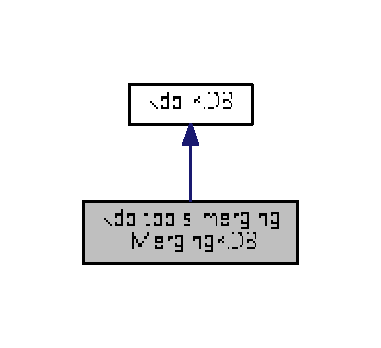
\includegraphics[width=191pt]{classkdb_1_1tools_1_1merging_1_1MergingKDB__inherit__graph}
\end{center}
\end{figure}


Collaboration diagram for kdb\+::tools\+::merging\+::Merging\+KDB\+:
\nopagebreak
\begin{figure}[H]
\begin{center}
\leavevmode
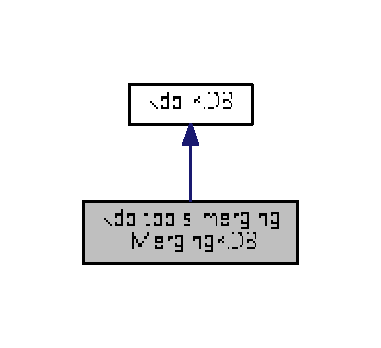
\includegraphics[width=191pt]{classkdb_1_1tools_1_1merging_1_1MergingKDB__coll__graph}
\end{center}
\end{figure}
\doxysubsection*{Public Member Functions}
\begin{DoxyCompactItemize}
\item 
int \mbox{\hyperlink{classkdb_1_1tools_1_1merging_1_1MergingKDB_a0d2a28f24aeb6ba3e81af73ef8b98df7}{get}} (\mbox{\hyperlink{classkdb_1_1KeySet}{Key\+Set}} \&returned, std\+::string const \&keyname) override
\begin{DoxyCompactList}\small\item\em Behaves like the \mbox{\hyperlink{classkdb_1_1KDB}{KDB}} get function. \end{DoxyCompactList}\item 
int \mbox{\hyperlink{classkdb_1_1tools_1_1merging_1_1MergingKDB_a062b1dac733aa3999691f8d70635b09c}{get}} (\mbox{\hyperlink{classkdb_1_1KeySet}{Key\+Set}} \&returned, \mbox{\hyperlink{classkdb_1_1Key}{Key}} \&parent\+Key) override
\begin{DoxyCompactList}\small\item\em Behaves like the \mbox{\hyperlink{classkdb_1_1KDB}{KDB}} get function. \end{DoxyCompactList}\item 
virtual int \mbox{\hyperlink{classkdb_1_1tools_1_1merging_1_1MergingKDB_ae7fb5bd354d16ed90bbf0c4c087b5d6f}{synchronize}} (\mbox{\hyperlink{classkdb_1_1KeySet}{Key\+Set}} \&returned, std\+::string const \&keyname, Three\+Way\+Merge \&merger)
\begin{DoxyCompactList}\small\item\em Synchronizes the file with the supplied \mbox{\hyperlink{classkdb_1_1KeySet}{Key\+Set}}. \end{DoxyCompactList}\item 
virtual int \mbox{\hyperlink{classkdb_1_1tools_1_1merging_1_1MergingKDB_adcb436c4bf35c89c67ae2f5b3f1a9cfd}{synchronize}} (\mbox{\hyperlink{classkdb_1_1KeySet}{Key\+Set}} \&returned, \mbox{\hyperlink{classkdb_1_1Key}{Key}} \&parent\+Key, Three\+Way\+Merge \&merger)
\begin{DoxyCompactList}\small\item\em If a conflict occurs during set, the supplied merger is used to resolve the conflict. \end{DoxyCompactList}\end{DoxyCompactItemize}


\doxysubsection{Detailed Description}
Provides a merging wrapper around a \mbox{\hyperlink{classkdb_1_1KDB}{KDB}} instance. 

The wrapper allows to pass a three way merger instance that is used to resolve conflicts during \mbox{\hyperlink{classkdb_1_1KDB}{KDB}} set. 

\doxysubsection{Member Function Documentation}
\mbox{\Hypertarget{classkdb_1_1tools_1_1merging_1_1MergingKDB_a062b1dac733aa3999691f8d70635b09c}\label{classkdb_1_1tools_1_1merging_1_1MergingKDB_a062b1dac733aa3999691f8d70635b09c}} 
\index{kdb::tools::merging::MergingKDB@{kdb::tools::merging::MergingKDB}!get@{get}}
\index{get@{get}!kdb::tools::merging::MergingKDB@{kdb::tools::merging::MergingKDB}}
\doxysubsubsection{\texorpdfstring{get()}{get()}\hspace{0.1cm}{\footnotesize\ttfamily [1/2]}}
{\footnotesize\ttfamily int kdb\+::tools\+::merging\+::\+Merging\+KDB\+::get (\begin{DoxyParamCaption}\item[{\mbox{\hyperlink{classkdb_1_1KeySet}{Key\+Set}} \&}]{returned,  }\item[{\mbox{\hyperlink{classkdb_1_1Key}{Key}} \&}]{parent\+Key }\end{DoxyParamCaption})\hspace{0.3cm}{\ttfamily [override]}, {\ttfamily [virtual]}}



Behaves like the \mbox{\hyperlink{classkdb_1_1KDB}{KDB}} get function. 

\begin{DoxySeeAlso}{See also}
\mbox{\hyperlink{classkdb_1_1KDB}{KDB}} 
\end{DoxySeeAlso}


Reimplemented from \mbox{\hyperlink{classkdb_1_1KDB_a48770a7290699bf2b7529f3ab67e378f}{kdb\+::\+KDB}}.

\mbox{\Hypertarget{classkdb_1_1tools_1_1merging_1_1MergingKDB_a0d2a28f24aeb6ba3e81af73ef8b98df7}\label{classkdb_1_1tools_1_1merging_1_1MergingKDB_a0d2a28f24aeb6ba3e81af73ef8b98df7}} 
\index{kdb::tools::merging::MergingKDB@{kdb::tools::merging::MergingKDB}!get@{get}}
\index{get@{get}!kdb::tools::merging::MergingKDB@{kdb::tools::merging::MergingKDB}}
\doxysubsubsection{\texorpdfstring{get()}{get()}\hspace{0.1cm}{\footnotesize\ttfamily [2/2]}}
{\footnotesize\ttfamily int kdb\+::tools\+::merging\+::\+Merging\+KDB\+::get (\begin{DoxyParamCaption}\item[{\mbox{\hyperlink{classkdb_1_1KeySet}{Key\+Set}} \&}]{returned,  }\item[{std\+::string const \&}]{keyname }\end{DoxyParamCaption})\hspace{0.3cm}{\ttfamily [override]}, {\ttfamily [virtual]}}



Behaves like the \mbox{\hyperlink{classkdb_1_1KDB}{KDB}} get function. 

\begin{DoxySeeAlso}{See also}
\mbox{\hyperlink{classkdb_1_1KDB}{KDB}} 
\end{DoxySeeAlso}


Reimplemented from \mbox{\hyperlink{classkdb_1_1KDB_a0419ffbc273c89756bc523b4223ec25a}{kdb\+::\+KDB}}.

\mbox{\Hypertarget{classkdb_1_1tools_1_1merging_1_1MergingKDB_adcb436c4bf35c89c67ae2f5b3f1a9cfd}\label{classkdb_1_1tools_1_1merging_1_1MergingKDB_adcb436c4bf35c89c67ae2f5b3f1a9cfd}} 
\index{kdb::tools::merging::MergingKDB@{kdb::tools::merging::MergingKDB}!synchronize@{synchronize}}
\index{synchronize@{synchronize}!kdb::tools::merging::MergingKDB@{kdb::tools::merging::MergingKDB}}
\doxysubsubsection{\texorpdfstring{synchronize()}{synchronize()}\hspace{0.1cm}{\footnotesize\ttfamily [1/2]}}
{\footnotesize\ttfamily int kdb\+::tools\+::merging\+::\+Merging\+KDB\+::synchronize (\begin{DoxyParamCaption}\item[{\mbox{\hyperlink{classkdb_1_1KeySet}{Key\+Set}} \&}]{returned,  }\item[{\mbox{\hyperlink{classkdb_1_1Key}{Key}} \&}]{parent\+Key,  }\item[{Three\+Way\+Merge \&}]{merger }\end{DoxyParamCaption})\hspace{0.3cm}{\ttfamily [virtual]}}



If a conflict occurs during set, the supplied merger is used to resolve the conflict. 

If the conflict cannot be solved, an exception is thrown. If the \mbox{\hyperlink{classkdb_1_1KeySet}{Key\+Set}} was successfully written (either by merging or due the absence of a conflict) the supplied \mbox{\hyperlink{classkdb_1_1KeySet}{Key\+Set}} is updated with the new content of the file.

\begin{DoxySeeAlso}{See also}
\mbox{\hyperlink{classkdb_1_1KDB}{KDB}} 
\end{DoxySeeAlso}

\begin{DoxyExceptions}{Exceptions}
{\em Merging\+KDBException} & \\
\hline
\end{DoxyExceptions}
\mbox{\Hypertarget{classkdb_1_1tools_1_1merging_1_1MergingKDB_ae7fb5bd354d16ed90bbf0c4c087b5d6f}\label{classkdb_1_1tools_1_1merging_1_1MergingKDB_ae7fb5bd354d16ed90bbf0c4c087b5d6f}} 
\index{kdb::tools::merging::MergingKDB@{kdb::tools::merging::MergingKDB}!synchronize@{synchronize}}
\index{synchronize@{synchronize}!kdb::tools::merging::MergingKDB@{kdb::tools::merging::MergingKDB}}
\doxysubsubsection{\texorpdfstring{synchronize()}{synchronize()}\hspace{0.1cm}{\footnotesize\ttfamily [2/2]}}
{\footnotesize\ttfamily int kdb\+::tools\+::merging\+::\+Merging\+KDB\+::synchronize (\begin{DoxyParamCaption}\item[{\mbox{\hyperlink{classkdb_1_1KeySet}{Key\+Set}} \&}]{returned,  }\item[{std\+::string const \&}]{keyname,  }\item[{Three\+Way\+Merge \&}]{merger }\end{DoxyParamCaption})\hspace{0.3cm}{\ttfamily [virtual]}}



Synchronizes the file with the supplied \mbox{\hyperlink{classkdb_1_1KeySet}{Key\+Set}}. 

If a conflict occurs during set, the supplied merger is used to resolve the conflict. If the conflict cannot be solved, an exception is thrown. If the \mbox{\hyperlink{classkdb_1_1KeySet}{Key\+Set}} was successfully written (either by merging or due the absence of a conflict) the supplied \mbox{\hyperlink{classkdb_1_1KeySet}{Key\+Set}} is updated with the new content of the file.

\begin{DoxySeeAlso}{See also}
\mbox{\hyperlink{classkdb_1_1KDB}{KDB}} 
\end{DoxySeeAlso}

\begin{DoxyExceptions}{Exceptions}
{\em Merging\+KDBException} & \\
\hline
\end{DoxyExceptions}


The documentation for this class was generated from the following files\+:\begin{DoxyCompactItemize}
\item 
\mbox{\hyperlink{mergingkdb_8hpp}{mergingkdb.\+hpp}}\item 
\mbox{\hyperlink{mergingkdb_8cpp}{mergingkdb.\+cpp}}\end{DoxyCompactItemize}

\hypertarget{classkdb_1_1tools_1_1MockPluginDatabase}{}\section{kdb\+:\+:tools\+:\+:Mock\+Plugin\+Database Class Reference}
\label{classkdb_1_1tools_1_1MockPluginDatabase}\index{kdb\+::tools\+::\+Mock\+Plugin\+Database@{kdb\+::tools\+::\+Mock\+Plugin\+Database}}


A plugin database that works with added fake data.  




{\ttfamily \#include $<$plugindatabase.\+hpp$>$}



Inheritance diagram for kdb\+:\+:tools\+:\+:Mock\+Plugin\+Database\+:
\nopagebreak
\begin{figure}[H]
\begin{center}
\leavevmode
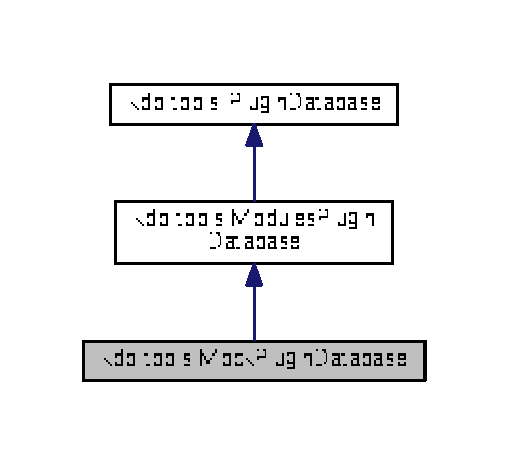
\includegraphics[width=244pt]{classkdb_1_1tools_1_1MockPluginDatabase__inherit__graph}
\end{center}
\end{figure}


Collaboration diagram for kdb\+:\+:tools\+:\+:Mock\+Plugin\+Database\+:
\nopagebreak
\begin{figure}[H]
\begin{center}
\leavevmode
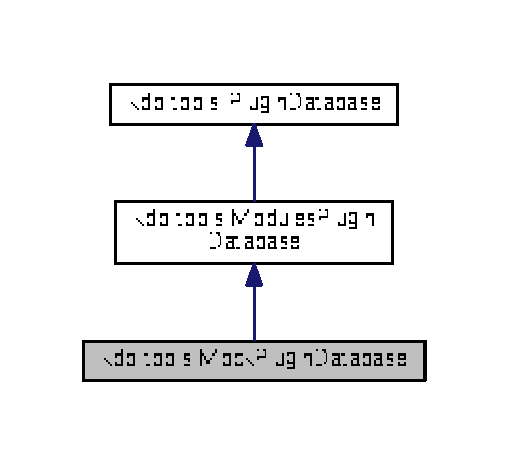
\includegraphics[width=244pt]{classkdb_1_1tools_1_1MockPluginDatabase__coll__graph}
\end{center}
\end{figure}
\subsection*{Public Member Functions}
\begin{DoxyCompactItemize}
\item 
std\+::vector$<$ std\+::string $>$ \hyperlink{classkdb_1_1tools_1_1MockPluginDatabase_a3663848683953bfad7123c48c00ab404}{list\+All\+Plugins} () const
\begin{DoxyCompactList}\small\item\em list all plugins \end{DoxyCompactList}\item 
std\+::string \hyperlink{classkdb_1_1tools_1_1MockPluginDatabase_ae352c27aa51bc8c2ea8c708d14f6fc76}{lookup\+Info} (\hyperlink{classkdb_1_1tools_1_1PluginSpec}{Plugin\+Spec} const \&spec, std\+::string const \&which) const
\begin{DoxyCompactList}\small\item\em lookup contract clauses or dynamic information \end{DoxyCompactList}\item 
func\+\_\+t \hyperlink{classkdb_1_1tools_1_1MockPluginDatabase_a5a701fd310be0e9f7d14a865c0226517}{get\+Symbol} (\hyperlink{classkdb_1_1tools_1_1PluginSpec}{Plugin\+Spec} const \&whichplugin, std\+::string const \&which) const
\begin{DoxyCompactList}\small\item\em get exported plugin symbol \end{DoxyCompactList}\end{DoxyCompactItemize}
\subsection*{Public Attributes}
\begin{DoxyCompactItemize}
\item 
std\+::unordered\+\_\+map$<$ \hyperlink{classkdb_1_1tools_1_1PluginSpec}{Plugin\+Spec}, std\+::unordered\+\_\+map$<$ std\+::string, std\+::string $>$, \hyperlink{structkdb_1_1tools_1_1PluginSpecHash}{Plugin\+Spec\+Hash}, Plugin\+Spec\+Name $>$ \hyperlink{classkdb_1_1tools_1_1MockPluginDatabase_a5de7756d9e7fb78d53903c92208d7fbe}{data}
\begin{DoxyCompactList}\small\item\em only data from here will be returned \end{DoxyCompactList}\end{DoxyCompactItemize}
\subsection*{Additional Inherited Members}


\subsection{Detailed Description}
A plugin database that works with added fake data. 

\subsection{Member Function Documentation}
\mbox{\Hypertarget{classkdb_1_1tools_1_1MockPluginDatabase_a5a701fd310be0e9f7d14a865c0226517}\label{classkdb_1_1tools_1_1MockPluginDatabase_a5a701fd310be0e9f7d14a865c0226517}} 
\index{kdb\+::tools\+::\+Mock\+Plugin\+Database@{kdb\+::tools\+::\+Mock\+Plugin\+Database}!get\+Symbol@{get\+Symbol}}
\index{get\+Symbol@{get\+Symbol}!kdb\+::tools\+::\+Mock\+Plugin\+Database@{kdb\+::tools\+::\+Mock\+Plugin\+Database}}
\subsubsection{\texorpdfstring{get\+Symbol()}{getSymbol()}}
{\footnotesize\ttfamily Plugin\+Database\+::func\+\_\+t kdb\+::tools\+::\+Mock\+Plugin\+Database\+::get\+Symbol (\begin{DoxyParamCaption}\item[{\hyperlink{classkdb_1_1tools_1_1PluginSpec}{Plugin\+Spec} const \&}]{whichplugin,  }\item[{std\+::string const \&}]{which }\end{DoxyParamCaption}) const\hspace{0.3cm}{\ttfamily [virtual]}}



get exported plugin symbol 


\begin{DoxyParams}{Parameters}
{\em whichplugin} & from which plugin? \\
\hline
{\em which} & which symbol would you like to look up?\\
\hline
\end{DoxyParams}
\begin{DoxyReturn}{Returns}
the function pointer to the exported symbol or N\+U\+LL if the symbol was not found 
\end{DoxyReturn}


Reimplemented from \hyperlink{classkdb_1_1tools_1_1ModulesPluginDatabase_a0e81e1b7b296a52f8040fd966b461c3a}{kdb\+::tools\+::\+Modules\+Plugin\+Database}.

\mbox{\Hypertarget{classkdb_1_1tools_1_1MockPluginDatabase_a3663848683953bfad7123c48c00ab404}\label{classkdb_1_1tools_1_1MockPluginDatabase_a3663848683953bfad7123c48c00ab404}} 
\index{kdb\+::tools\+::\+Mock\+Plugin\+Database@{kdb\+::tools\+::\+Mock\+Plugin\+Database}!list\+All\+Plugins@{list\+All\+Plugins}}
\index{list\+All\+Plugins@{list\+All\+Plugins}!kdb\+::tools\+::\+Mock\+Plugin\+Database@{kdb\+::tools\+::\+Mock\+Plugin\+Database}}
\subsubsection{\texorpdfstring{list\+All\+Plugins()}{listAllPlugins()}}
{\footnotesize\ttfamily std\+::vector$<$ std\+::string $>$ kdb\+::tools\+::\+Mock\+Plugin\+Database\+::list\+All\+Plugins (\begin{DoxyParamCaption}{ }\end{DoxyParamCaption}) const\hspace{0.3cm}{\ttfamily [virtual]}}



list all plugins 

If Elektra is compiled with plugins, it will search for shared libraries. In any case, if no shared libraries were found it will fallback to an internal list (plugins that were compiled together with Elektra).

\begin{DoxyReturn}{Returns}
a list of all available plugins 
\end{DoxyReturn}


Reimplemented from \hyperlink{classkdb_1_1tools_1_1ModulesPluginDatabase_a3fa5a08caf47cb79f9889641a96f197b}{kdb\+::tools\+::\+Modules\+Plugin\+Database}.

\mbox{\Hypertarget{classkdb_1_1tools_1_1MockPluginDatabase_ae352c27aa51bc8c2ea8c708d14f6fc76}\label{classkdb_1_1tools_1_1MockPluginDatabase_ae352c27aa51bc8c2ea8c708d14f6fc76}} 
\index{kdb\+::tools\+::\+Mock\+Plugin\+Database@{kdb\+::tools\+::\+Mock\+Plugin\+Database}!lookup\+Info@{lookup\+Info}}
\index{lookup\+Info@{lookup\+Info}!kdb\+::tools\+::\+Mock\+Plugin\+Database@{kdb\+::tools\+::\+Mock\+Plugin\+Database}}
\subsubsection{\texorpdfstring{lookup\+Info()}{lookupInfo()}}
{\footnotesize\ttfamily std\+::string kdb\+::tools\+::\+Mock\+Plugin\+Database\+::lookup\+Info (\begin{DoxyParamCaption}\item[{\hyperlink{classkdb_1_1tools_1_1PluginSpec}{Plugin\+Spec} const \&}]{whichplugin,  }\item[{std\+::string const \&}]{which }\end{DoxyParamCaption}) const\hspace{0.3cm}{\ttfamily [virtual]}}



lookup contract clauses or dynamic information 


\begin{DoxyParams}{Parameters}
{\em whichplugin} & about which plugin? \\
\hline
{\em which} & about which clause in the contract?\\
\hline
\end{DoxyParams}
\begin{DoxyReturn}{Returns}
the clause of the contract 
\end{DoxyReturn}


Reimplemented from \hyperlink{classkdb_1_1tools_1_1ModulesPluginDatabase_a3f51beee8aecb4371e7d12e98958f875}{kdb\+::tools\+::\+Modules\+Plugin\+Database}.



\subsection{Member Data Documentation}
\mbox{\Hypertarget{classkdb_1_1tools_1_1MockPluginDatabase_a5de7756d9e7fb78d53903c92208d7fbe}\label{classkdb_1_1tools_1_1MockPluginDatabase_a5de7756d9e7fb78d53903c92208d7fbe}} 
\index{kdb\+::tools\+::\+Mock\+Plugin\+Database@{kdb\+::tools\+::\+Mock\+Plugin\+Database}!data@{data}}
\index{data@{data}!kdb\+::tools\+::\+Mock\+Plugin\+Database@{kdb\+::tools\+::\+Mock\+Plugin\+Database}}
\subsubsection{\texorpdfstring{data}{data}}
{\footnotesize\ttfamily std\+::unordered\+\_\+map$<$\hyperlink{classkdb_1_1tools_1_1PluginSpec}{Plugin\+Spec}, std\+::unordered\+\_\+map$<$std\+::string, std\+::string$>$, \hyperlink{structkdb_1_1tools_1_1PluginSpecHash}{Plugin\+Spec\+Hash}, Plugin\+Spec\+Name$>$ kdb\+::tools\+::\+Mock\+Plugin\+Database\+::data\hspace{0.3cm}{\ttfamily [mutable]}}



only data from here will be returned 

\begin{DoxyNote}{Note}
that it is ordered by name, i.\+e., different ref-\/names cannot be distinguished 
\end{DoxyNote}


The documentation for this class was generated from the following files\+:\begin{DoxyCompactItemize}
\item 
\hyperlink{plugindatabase_8hpp}{plugindatabase.\+hpp}\item 
\hyperlink{plugindatabase_8cpp}{plugindatabase.\+cpp}\end{DoxyCompactItemize}

\hypertarget{classkdb_1_1tools_1_1Modules}{\section{kdb\+:\+:tools\+:\+:Modules Class Reference}
\label{classkdb_1_1tools_1_1Modules}\index{kdb\+::tools\+::\+Modules@{kdb\+::tools\+::\+Modules}}
}


Allows one to load plugins.  




{\ttfamily \#include $<$modules.\+hpp$>$}

\subsection*{Public Member Functions}
\begin{DoxyCompactItemize}
\item 
Plugin\+Ptr \hyperlink{classkdb_1_1tools_1_1Modules_ae8d8c91745c9f517e6e8a556f1664f69}{load} (std\+::string const \&plugin\+Name)
\item 
Plugin\+Ptr \hyperlink{classkdb_1_1tools_1_1Modules_a6ae72cc8e30fe3fb0aabd6f78fad8ddf}{load} (std\+::string const \&plugin\+Name, \hyperlink{classkdb_1_1KeySet}{kdb\+::\+Key\+Set} const \&config)
\item 
Plugin\+Ptr \hyperlink{classkdb_1_1tools_1_1Modules_abdbcc54896557ad3123d0a12be9f437a}{load} (\hyperlink{classkdb_1_1tools_1_1PluginSpec}{Plugin\+Spec} const \&spec)
\end{DoxyCompactItemize}


\subsection{Detailed Description}
Allows one to load plugins. 

\subsection{Member Function Documentation}
\hypertarget{classkdb_1_1tools_1_1Modules_ae8d8c91745c9f517e6e8a556f1664f69}{\index{kdb\+::tools\+::\+Modules@{kdb\+::tools\+::\+Modules}!load@{load}}
\index{load@{load}!kdb\+::tools\+::\+Modules@{kdb\+::tools\+::\+Modules}}
\subsubsection[{load}]{\setlength{\rightskip}{0pt plus 5cm}Plugin\+Ptr kdb\+::tools\+::\+Modules\+::load (
\begin{DoxyParamCaption}
\item[{std\+::string const \&}]{plugin\+Name}
\end{DoxyParamCaption}
)}}\label{classkdb_1_1tools_1_1Modules_ae8d8c91745c9f517e6e8a556f1664f69}
\begin{DoxyRefDesc}{Deprecated}
\item[\hyperlink{deprecated__deprecated000026}{Deprecated}]do not use \end{DoxyRefDesc}
\hypertarget{classkdb_1_1tools_1_1Modules_a6ae72cc8e30fe3fb0aabd6f78fad8ddf}{\index{kdb\+::tools\+::\+Modules@{kdb\+::tools\+::\+Modules}!load@{load}}
\index{load@{load}!kdb\+::tools\+::\+Modules@{kdb\+::tools\+::\+Modules}}
\subsubsection[{load}]{\setlength{\rightskip}{0pt plus 5cm}Plugin\+Ptr kdb\+::tools\+::\+Modules\+::load (
\begin{DoxyParamCaption}
\item[{std\+::string const \&}]{plugin\+Name, }
\item[{{\bf kdb\+::\+Key\+Set} const \&}]{config}
\end{DoxyParamCaption}
)}}\label{classkdb_1_1tools_1_1Modules_a6ae72cc8e30fe3fb0aabd6f78fad8ddf}
\begin{DoxyRefDesc}{Deprecated}
\item[\hyperlink{deprecated__deprecated000027}{Deprecated}]do not use \end{DoxyRefDesc}
\hypertarget{classkdb_1_1tools_1_1Modules_abdbcc54896557ad3123d0a12be9f437a}{\index{kdb\+::tools\+::\+Modules@{kdb\+::tools\+::\+Modules}!load@{load}}
\index{load@{load}!kdb\+::tools\+::\+Modules@{kdb\+::tools\+::\+Modules}}
\subsubsection[{load}]{\setlength{\rightskip}{0pt plus 5cm}Plugin\+Ptr kdb\+::tools\+::\+Modules\+::load (
\begin{DoxyParamCaption}
\item[{{\bf Plugin\+Spec} const \&}]{spec}
\end{DoxyParamCaption}
)}}\label{classkdb_1_1tools_1_1Modules_abdbcc54896557ad3123d0a12be9f437a}
\begin{DoxyReturn}{Returns}
a newly created plugin 
\end{DoxyReturn}


The documentation for this class was generated from the following files\+:\begin{DoxyCompactItemize}
\item 
\hyperlink{modules_8hpp}{modules.\+hpp}\item 
\hyperlink{modules_8cpp}{modules.\+cpp}\end{DoxyCompactItemize}

\hypertarget{classkdb_1_1tools_1_1ModulesPluginDatabase}{}\doxysection{kdb\+::tools\+::Modules\+Plugin\+Database Class Reference}
\label{classkdb_1_1tools_1_1ModulesPluginDatabase}\index{kdb::tools::ModulesPluginDatabase@{kdb::tools::ModulesPluginDatabase}}


A plugin database that works with installed modules.  




{\ttfamily \#include $<$plugindatabase.\+hpp$>$}



Inheritance diagram for kdb\+::tools\+::Modules\+Plugin\+Database\+:
\nopagebreak
\begin{figure}[H]
\begin{center}
\leavevmode
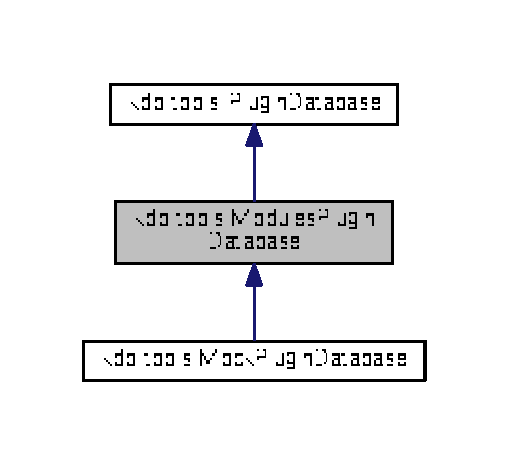
\includegraphics[width=253pt]{classkdb_1_1tools_1_1ModulesPluginDatabase__inherit__graph}
\end{center}
\end{figure}


Collaboration diagram for kdb\+::tools\+::Modules\+Plugin\+Database\+:
\nopagebreak
\begin{figure}[H]
\begin{center}
\leavevmode
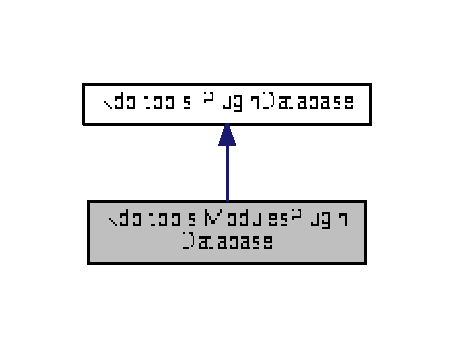
\includegraphics[width=227pt]{classkdb_1_1tools_1_1ModulesPluginDatabase__coll__graph}
\end{center}
\end{figure}
\doxysubsection*{Public Member Functions}
\begin{DoxyCompactItemize}
\item 
std\+::vector$<$ std\+::string $>$ \mbox{\hyperlink{classkdb_1_1tools_1_1ModulesPluginDatabase_a3fa5a08caf47cb79f9889641a96f197b}{list\+All\+Plugins}} () const
\begin{DoxyCompactList}\small\item\em list all plugins \end{DoxyCompactList}\item 
std\+::string \mbox{\hyperlink{classkdb_1_1tools_1_1ModulesPluginDatabase_a3f51beee8aecb4371e7d12e98958f875}{lookup\+Info}} (\mbox{\hyperlink{classkdb_1_1tools_1_1PluginSpec}{Plugin\+Spec}} const \&spec, std\+::string const \&which) const
\begin{DoxyCompactList}\small\item\em lookup contract clauses or dynamic information \end{DoxyCompactList}\item 
func\+\_\+t \mbox{\hyperlink{classkdb_1_1tools_1_1ModulesPluginDatabase_a0e81e1b7b296a52f8040fd966b461c3a}{get\+Symbol}} (\mbox{\hyperlink{classkdb_1_1tools_1_1PluginSpec}{Plugin\+Spec}} const \&whichplugin, std\+::string const \&which) const
\begin{DoxyCompactList}\small\item\em get exported plugin symbol \end{DoxyCompactList}\item 
\mbox{\hyperlink{classkdb_1_1tools_1_1PluginSpec}{Plugin\+Spec}} \mbox{\hyperlink{classkdb_1_1tools_1_1ModulesPluginDatabase_aa7f244f0271ea9b2a3f5b52779167f55}{lookup\+Metadata}} (std\+::string const \&which) const
\begin{DoxyCompactList}\small\item\em lookup which plugin handles metadata \end{DoxyCompactList}\item 
\mbox{\hyperlink{classkdb_1_1tools_1_1PluginSpec}{Plugin\+Spec}} \mbox{\hyperlink{classkdb_1_1tools_1_1ModulesPluginDatabase_acdb15c10fc34f74687ecbbf8bac526f6}{lookup\+Provides}} (std\+::string const \&\mbox{\hyperlink{classkdb_1_1tools_1_1PluginDatabase_afc91ff760616ee83c6afb70e5a2f0601a73ff10d6a07213c277db4326b3df6c4b}{provides}}) const
\begin{DoxyCompactList}\small\item\em lookup which plugin is a provider for that plugin \end{DoxyCompactList}\item 
std\+::map$<$ int, \mbox{\hyperlink{classkdb_1_1tools_1_1PluginSpec}{Plugin\+Spec}} $>$ \mbox{\hyperlink{classkdb_1_1tools_1_1ModulesPluginDatabase_abe19487ff2a2e0548288dfa2a5678ae1}{lookup\+All\+Provides\+With\+Status}} (std\+::string const \&\mbox{\hyperlink{classkdb_1_1tools_1_1PluginDatabase_afc91ff760616ee83c6afb70e5a2f0601a73ff10d6a07213c277db4326b3df6c4b}{provides}}) const
\begin{DoxyCompactList}\small\item\em looks up all plugins which are a suitable provider \end{DoxyCompactList}\item 
std\+::vector$<$ \mbox{\hyperlink{classkdb_1_1tools_1_1PluginSpec}{Plugin\+Spec}} $>$ \mbox{\hyperlink{classkdb_1_1tools_1_1ModulesPluginDatabase_a306384e88f9cf2874f6ba9ce28973a26}{lookup\+All\+Provides}} (std\+::string const \&\mbox{\hyperlink{classkdb_1_1tools_1_1PluginDatabase_afc91ff760616ee83c6afb70e5a2f0601a73ff10d6a07213c277db4326b3df6c4b}{provides}}) const
\begin{DoxyCompactList}\small\item\em looks up all plugins which are a suitable provider \end{DoxyCompactList}\end{DoxyCompactItemize}
\doxysubsection*{Additional Inherited Members}


\doxysubsection{Detailed Description}
A plugin database that works with installed modules. 

\doxysubsection{Member Function Documentation}
\mbox{\Hypertarget{classkdb_1_1tools_1_1ModulesPluginDatabase_a0e81e1b7b296a52f8040fd966b461c3a}\label{classkdb_1_1tools_1_1ModulesPluginDatabase_a0e81e1b7b296a52f8040fd966b461c3a}} 
\index{kdb::tools::ModulesPluginDatabase@{kdb::tools::ModulesPluginDatabase}!getSymbol@{getSymbol}}
\index{getSymbol@{getSymbol}!kdb::tools::ModulesPluginDatabase@{kdb::tools::ModulesPluginDatabase}}
\doxysubsubsection{\texorpdfstring{getSymbol()}{getSymbol()}}
{\footnotesize\ttfamily Plugin\+Database\+::func\+\_\+t kdb\+::tools\+::\+Modules\+Plugin\+Database\+::get\+Symbol (\begin{DoxyParamCaption}\item[{\mbox{\hyperlink{classkdb_1_1tools_1_1PluginSpec}{Plugin\+Spec}} const \&}]{whichplugin,  }\item[{std\+::string const \&}]{which }\end{DoxyParamCaption}) const\hspace{0.3cm}{\ttfamily [virtual]}}



get exported plugin symbol 


\begin{DoxyParams}{Parameters}
{\em whichplugin} & from which plugin? \\
\hline
{\em which} & which symbol would you like to look up?\\
\hline
\end{DoxyParams}
\begin{DoxyReturn}{Returns}
the function pointer to the exported symbol or N\+U\+LL if the symbol was not found 
\end{DoxyReturn}


Implements \mbox{\hyperlink{classkdb_1_1tools_1_1PluginDatabase_a87b5ef6ee66ce1ad46cc590a2b60b9fa}{kdb\+::tools\+::\+Plugin\+Database}}.



Reimplemented in \mbox{\hyperlink{classkdb_1_1tools_1_1MockPluginDatabase_a5a701fd310be0e9f7d14a865c0226517}{kdb\+::tools\+::\+Mock\+Plugin\+Database}}.

\mbox{\Hypertarget{classkdb_1_1tools_1_1ModulesPluginDatabase_a3fa5a08caf47cb79f9889641a96f197b}\label{classkdb_1_1tools_1_1ModulesPluginDatabase_a3fa5a08caf47cb79f9889641a96f197b}} 
\index{kdb::tools::ModulesPluginDatabase@{kdb::tools::ModulesPluginDatabase}!listAllPlugins@{listAllPlugins}}
\index{listAllPlugins@{listAllPlugins}!kdb::tools::ModulesPluginDatabase@{kdb::tools::ModulesPluginDatabase}}
\doxysubsubsection{\texorpdfstring{listAllPlugins()}{listAllPlugins()}}
{\footnotesize\ttfamily std\+::vector$<$ std\+::string $>$ kdb\+::tools\+::\+Modules\+Plugin\+Database\+::list\+All\+Plugins (\begin{DoxyParamCaption}{ }\end{DoxyParamCaption}) const\hspace{0.3cm}{\ttfamily [virtual]}}



list all plugins 

If Elektra is compiled with plugins, it will search for shared libraries. In any case, if no shared libraries were found it will fallback to an internal list (plugins that were compiled together with Elektra).

\begin{DoxyReturn}{Returns}
a list of all available plugins 
\end{DoxyReturn}


Implements \mbox{\hyperlink{classkdb_1_1tools_1_1PluginDatabase_adc1f43ccefdd7fc15a57db7571420642}{kdb\+::tools\+::\+Plugin\+Database}}.



Reimplemented in \mbox{\hyperlink{classkdb_1_1tools_1_1MockPluginDatabase_a3663848683953bfad7123c48c00ab404}{kdb\+::tools\+::\+Mock\+Plugin\+Database}}.

\mbox{\Hypertarget{classkdb_1_1tools_1_1ModulesPluginDatabase_a306384e88f9cf2874f6ba9ce28973a26}\label{classkdb_1_1tools_1_1ModulesPluginDatabase_a306384e88f9cf2874f6ba9ce28973a26}} 
\index{kdb::tools::ModulesPluginDatabase@{kdb::tools::ModulesPluginDatabase}!lookupAllProvides@{lookupAllProvides}}
\index{lookupAllProvides@{lookupAllProvides}!kdb::tools::ModulesPluginDatabase@{kdb::tools::ModulesPluginDatabase}}
\doxysubsubsection{\texorpdfstring{lookupAllProvides()}{lookupAllProvides()}}
{\footnotesize\ttfamily std\+::vector$<$ \mbox{\hyperlink{classkdb_1_1tools_1_1PluginSpec}{Plugin\+Spec}} $>$ kdb\+::tools\+::\+Modules\+Plugin\+Database\+::lookup\+All\+Provides (\begin{DoxyParamCaption}\item[{std\+::string const \&}]{provides }\end{DoxyParamCaption}) const\hspace{0.3cm}{\ttfamily [virtual]}}



looks up all plugins which are a suitable provider 

\begin{DoxyNote}{Note}
in case a plugin name is provided, the plugin with the name will also be part of the result. But if there are other plugins providing the requirement, then they will also be part of the result. The ordering of the resulting vector has no special meaning.
\end{DoxyNote}

\begin{DoxyParams}{Parameters}
{\em provides} & is the provider to find\\
\hline
\end{DoxyParams}
\begin{DoxyReturn}{Returns}
a vector of plugins offering the requirement or are named after it 
\end{DoxyReturn}


Implements \mbox{\hyperlink{classkdb_1_1tools_1_1PluginDatabase_a3ed261ad8562c423b64cf34cbc086161}{kdb\+::tools\+::\+Plugin\+Database}}.

\mbox{\Hypertarget{classkdb_1_1tools_1_1ModulesPluginDatabase_abe19487ff2a2e0548288dfa2a5678ae1}\label{classkdb_1_1tools_1_1ModulesPluginDatabase_abe19487ff2a2e0548288dfa2a5678ae1}} 
\index{kdb::tools::ModulesPluginDatabase@{kdb::tools::ModulesPluginDatabase}!lookupAllProvidesWithStatus@{lookupAllProvidesWithStatus}}
\index{lookupAllProvidesWithStatus@{lookupAllProvidesWithStatus}!kdb::tools::ModulesPluginDatabase@{kdb::tools::ModulesPluginDatabase}}
\doxysubsubsection{\texorpdfstring{lookupAllProvidesWithStatus()}{lookupAllProvidesWithStatus()}}
{\footnotesize\ttfamily std\+::map$<$ int, \mbox{\hyperlink{classkdb_1_1tools_1_1PluginSpec}{Plugin\+Spec}} $>$ kdb\+::tools\+::\+Modules\+Plugin\+Database\+::lookup\+All\+Provides\+With\+Status (\begin{DoxyParamCaption}\item[{std\+::string const \&}]{provides }\end{DoxyParamCaption}) const\hspace{0.3cm}{\ttfamily [virtual]}}



looks up all plugins which are a suitable provider 

\begin{DoxyNote}{Note}
in case a plugin name is provided, the plugin with the name will also be part of the result. But if there are other plugins providing the requirement, then they will also be part of the result.
\end{DoxyNote}

\begin{DoxyParams}{Parameters}
{\em provides} & is the provider to find\\
\hline
\end{DoxyParams}
\begin{DoxyReturn}{Returns}
a map of plugins with their status offering the requirement or are named after it 
\end{DoxyReturn}


Implements \mbox{\hyperlink{classkdb_1_1tools_1_1PluginDatabase_aa918b547973f627a5604fa3b2b3faf30}{kdb\+::tools\+::\+Plugin\+Database}}.

\mbox{\Hypertarget{classkdb_1_1tools_1_1ModulesPluginDatabase_a3f51beee8aecb4371e7d12e98958f875}\label{classkdb_1_1tools_1_1ModulesPluginDatabase_a3f51beee8aecb4371e7d12e98958f875}} 
\index{kdb::tools::ModulesPluginDatabase@{kdb::tools::ModulesPluginDatabase}!lookupInfo@{lookupInfo}}
\index{lookupInfo@{lookupInfo}!kdb::tools::ModulesPluginDatabase@{kdb::tools::ModulesPluginDatabase}}
\doxysubsubsection{\texorpdfstring{lookupInfo()}{lookupInfo()}}
{\footnotesize\ttfamily std\+::string kdb\+::tools\+::\+Modules\+Plugin\+Database\+::lookup\+Info (\begin{DoxyParamCaption}\item[{\mbox{\hyperlink{classkdb_1_1tools_1_1PluginSpec}{Plugin\+Spec}} const \&}]{whichplugin,  }\item[{std\+::string const \&}]{which }\end{DoxyParamCaption}) const\hspace{0.3cm}{\ttfamily [virtual]}}



lookup contract clauses or dynamic information 


\begin{DoxyParams}{Parameters}
{\em whichplugin} & about which plugin? \\
\hline
{\em which} & about which clause in the contract?\\
\hline
\end{DoxyParams}
\begin{DoxyReturn}{Returns}
the clause of the contract 
\end{DoxyReturn}


Implements \mbox{\hyperlink{classkdb_1_1tools_1_1PluginDatabase_ac0af2ec31a98f4176c19eaf34977abbe}{kdb\+::tools\+::\+Plugin\+Database}}.



Reimplemented in \mbox{\hyperlink{classkdb_1_1tools_1_1MockPluginDatabase_ae352c27aa51bc8c2ea8c708d14f6fc76}{kdb\+::tools\+::\+Mock\+Plugin\+Database}}.

\mbox{\Hypertarget{classkdb_1_1tools_1_1ModulesPluginDatabase_aa7f244f0271ea9b2a3f5b52779167f55}\label{classkdb_1_1tools_1_1ModulesPluginDatabase_aa7f244f0271ea9b2a3f5b52779167f55}} 
\index{kdb::tools::ModulesPluginDatabase@{kdb::tools::ModulesPluginDatabase}!lookupMetadata@{lookupMetadata}}
\index{lookupMetadata@{lookupMetadata}!kdb::tools::ModulesPluginDatabase@{kdb::tools::ModulesPluginDatabase}}
\doxysubsubsection{\texorpdfstring{lookupMetadata()}{lookupMetadata()}}
{\footnotesize\ttfamily \mbox{\hyperlink{classkdb_1_1tools_1_1PluginSpec}{Plugin\+Spec}} kdb\+::tools\+::\+Modules\+Plugin\+Database\+::lookup\+Metadata (\begin{DoxyParamCaption}\item[{std\+::string const \&}]{which }\end{DoxyParamCaption}) const\hspace{0.3cm}{\ttfamily [virtual]}}



lookup which plugin handles metadata 


\begin{DoxyParams}{Parameters}
{\em which} & the metadata of interest\\
\hline
\end{DoxyParams}
\begin{DoxyReturn}{Returns}
the best suited plugin specification which provides it 
\end{DoxyReturn}


Implements \mbox{\hyperlink{classkdb_1_1tools_1_1PluginDatabase_a03a416f66d6525f46929e5a68d9db3f7}{kdb\+::tools\+::\+Plugin\+Database}}.

\mbox{\Hypertarget{classkdb_1_1tools_1_1ModulesPluginDatabase_acdb15c10fc34f74687ecbbf8bac526f6}\label{classkdb_1_1tools_1_1ModulesPluginDatabase_acdb15c10fc34f74687ecbbf8bac526f6}} 
\index{kdb::tools::ModulesPluginDatabase@{kdb::tools::ModulesPluginDatabase}!lookupProvides@{lookupProvides}}
\index{lookupProvides@{lookupProvides}!kdb::tools::ModulesPluginDatabase@{kdb::tools::ModulesPluginDatabase}}
\doxysubsubsection{\texorpdfstring{lookupProvides()}{lookupProvides()}}
{\footnotesize\ttfamily \mbox{\hyperlink{classkdb_1_1tools_1_1PluginSpec}{Plugin\+Spec}} kdb\+::tools\+::\+Modules\+Plugin\+Database\+::lookup\+Provides (\begin{DoxyParamCaption}\item[{std\+::string const \&}]{provides }\end{DoxyParamCaption}) const\hspace{0.3cm}{\ttfamily [virtual]}}



lookup which plugin is a provider for that plugin 

\begin{DoxyNote}{Note}
will return a \mbox{\hyperlink{classkdb_1_1tools_1_1PluginSpec}{Plugin\+Spec}} with get\+Name() == provides if the string provides actually is a plugin name.
\end{DoxyNote}

\begin{DoxyParams}{Parameters}
{\em provides} & is the provider to find\\
\hline
\end{DoxyParams}

\begin{DoxyExceptions}{Exceptions}
{\em No\+Plugin} & if no plugin that provides the functionality could be found\\
\hline
\end{DoxyExceptions}
\begin{DoxyReturn}{Returns}
the plugin itself or the best suited plugin specification which provides it 
\end{DoxyReturn}


Implements \mbox{\hyperlink{classkdb_1_1tools_1_1PluginDatabase_a43abe56a024218ecee48526ced699f05}{kdb\+::tools\+::\+Plugin\+Database}}.



The documentation for this class was generated from the following files\+:\begin{DoxyCompactItemize}
\item 
\mbox{\hyperlink{plugindatabase_8hpp}{plugindatabase.\+hpp}}\item 
\mbox{\hyperlink{plugindatabase_8cpp}{plugindatabase.\+cpp}}\end{DoxyCompactItemize}

\hypertarget{classkdb_1_1tools_1_1MountBackendBuilder}{}\section{kdb\+:\+:tools\+:\+:Mount\+Backend\+Builder Class Reference}
\label{classkdb_1_1tools_1_1MountBackendBuilder}\index{kdb\+::tools\+::\+Mount\+Backend\+Builder@{kdb\+::tools\+::\+Mount\+Backend\+Builder}}


High-\/level functionality to build a mountpoint.  




{\ttfamily \#include $<$backendbuilder.\+hpp$>$}



Inheritance diagram for kdb\+:\+:tools\+:\+:Mount\+Backend\+Builder\+:
\nopagebreak
\begin{figure}[H]
\begin{center}
\leavevmode
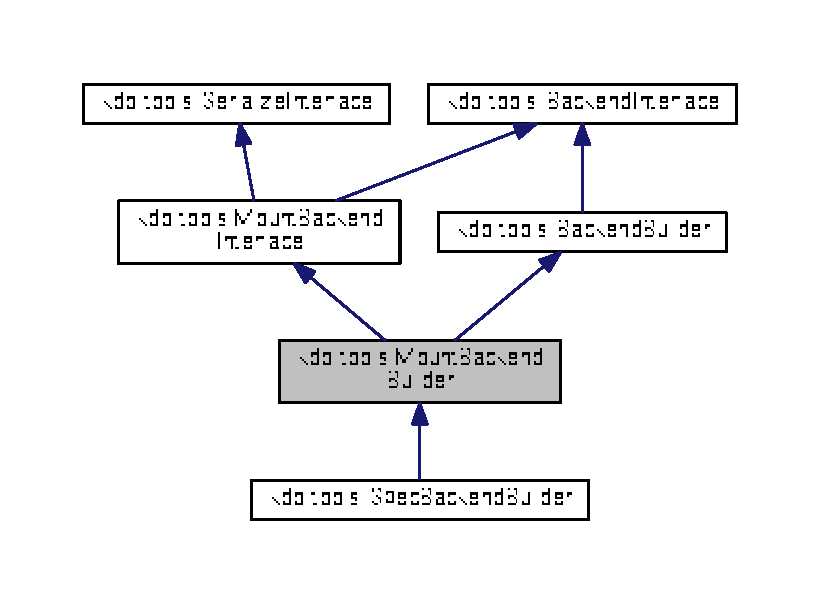
\includegraphics[width=350pt]{classkdb_1_1tools_1_1MountBackendBuilder__inherit__graph}
\end{center}
\end{figure}


Collaboration diagram for kdb\+:\+:tools\+:\+:Mount\+Backend\+Builder\+:
\nopagebreak
\begin{figure}[H]
\begin{center}
\leavevmode
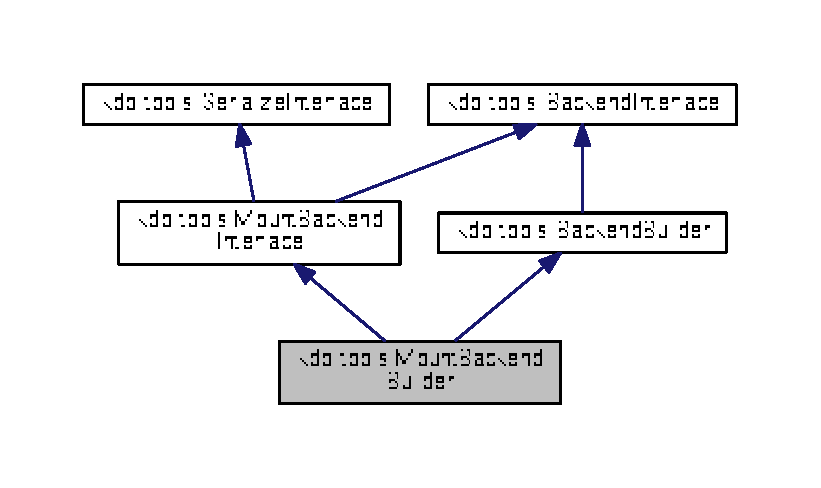
\includegraphics[width=350pt]{classkdb_1_1tools_1_1MountBackendBuilder__coll__graph}
\end{center}
\end{figure}
\subsection*{Public Member Functions}
\begin{DoxyCompactItemize}
\item 
void \hyperlink{classkdb_1_1tools_1_1MountBackendBuilder_a2603e75436a49fc66696c1b41b27efb9}{add\+Plugin} (\hyperlink{classkdb_1_1tools_1_1PluginSpec}{Plugin\+Spec} const \&spec)
\begin{DoxyCompactList}\small\item\em Add a plugin. \end{DoxyCompactList}\end{DoxyCompactItemize}


\subsection{Detailed Description}
High-\/level functionality to build a mountpoint. 

will enforce resolver and storage to be present 

\subsection{Member Function Documentation}
\mbox{\Hypertarget{classkdb_1_1tools_1_1MountBackendBuilder_a2603e75436a49fc66696c1b41b27efb9}\label{classkdb_1_1tools_1_1MountBackendBuilder_a2603e75436a49fc66696c1b41b27efb9}} 
\index{kdb\+::tools\+::\+Mount\+Backend\+Builder@{kdb\+::tools\+::\+Mount\+Backend\+Builder}!add\+Plugin@{add\+Plugin}}
\index{add\+Plugin@{add\+Plugin}!kdb\+::tools\+::\+Mount\+Backend\+Builder@{kdb\+::tools\+::\+Mount\+Backend\+Builder}}
\subsubsection{\texorpdfstring{add\+Plugin()}{addPlugin()}}
{\footnotesize\ttfamily void kdb\+::tools\+::\+Mount\+Backend\+Builder\+::add\+Plugin (\begin{DoxyParamCaption}\item[{\hyperlink{classkdb_1_1tools_1_1PluginSpec}{Plugin\+Spec} const \&}]{plugin }\end{DoxyParamCaption})\hspace{0.3cm}{\ttfamily [inline]}, {\ttfamily [virtual]}}



Add a plugin. 

\begin{DoxyPrecond}{Precondition}
Needs to be a unique new name (use refname if you want to add the same module multiple times)
\end{DoxyPrecond}
Will automatically resolve virtual plugins to actual plugins.

Also calls the checkconf function if provided by the plugin. The checkconf function has the following signature\+: int checkconf (\hyperlink{classkdb_1_1Key}{Key} $\ast$ error\+Key, \hyperlink{classkdb_1_1KeySet}{Key\+Set} $\ast$ config) and allows a plugin to verify its configuration at mount time.

\begin{DoxySeeAlso}{See also}
\hyperlink{classkdb_1_1tools_1_1BackendBuilder_a6e6c23716dc72ef68f8acfd71fc802a9}{resolve\+Needs()} 
\end{DoxySeeAlso}

\begin{DoxyParams}{Parameters}
{\em plugin} & \\
\hline
\end{DoxyParams}


Reimplemented from \hyperlink{classkdb_1_1tools_1_1BackendBuilder_a987d2c3711399e24b42c38e652c0e1c4}{kdb\+::tools\+::\+Backend\+Builder}.



The documentation for this class was generated from the following files\+:\begin{DoxyCompactItemize}
\item 
\hyperlink{backendbuilder_8hpp}{backendbuilder.\+hpp}\item 
\hyperlink{backendbuilder_8cpp}{backendbuilder.\+cpp}\end{DoxyCompactItemize}

\hypertarget{classkdb_1_1tools_1_1MountBackendInterface}{\section{kdb\+:\+:tools\+:\+:Mount\+Backend\+Interface Class Reference}
\label{classkdb_1_1tools_1_1MountBackendInterface}\index{kdb\+::tools\+::\+Mount\+Backend\+Interface@{kdb\+::tools\+::\+Mount\+Backend\+Interface}}
}


Interface to work with mountpoints (backends) for factory.  




{\ttfamily \#include $<$backend.\+hpp$>$}



Inheritance diagram for kdb\+:\+:tools\+:\+:Mount\+Backend\+Interface\+:
\nopagebreak
\begin{figure}[H]
\begin{center}
\leavevmode
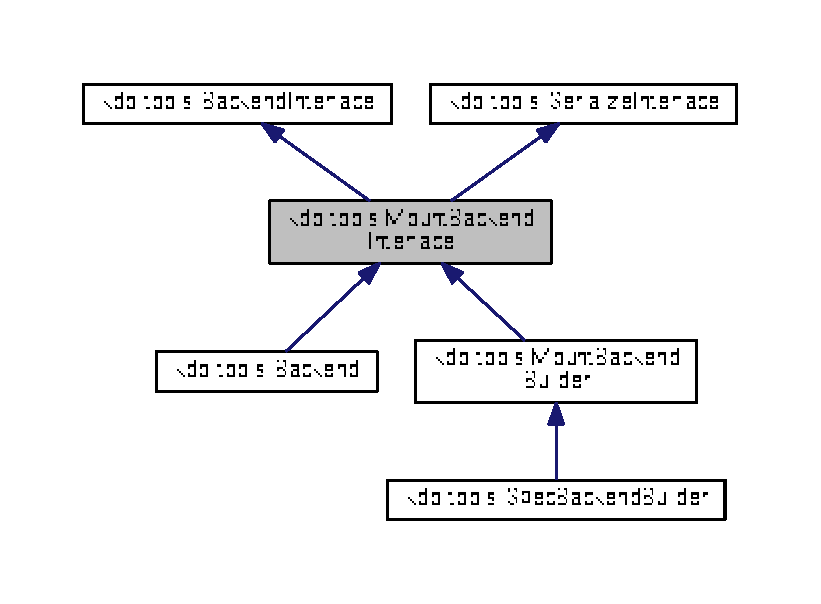
\includegraphics[width=350pt]{classkdb_1_1tools_1_1MountBackendInterface__inherit__graph}
\end{center}
\end{figure}


Collaboration diagram for kdb\+:\+:tools\+:\+:Mount\+Backend\+Interface\+:
\nopagebreak
\begin{figure}[H]
\begin{center}
\leavevmode
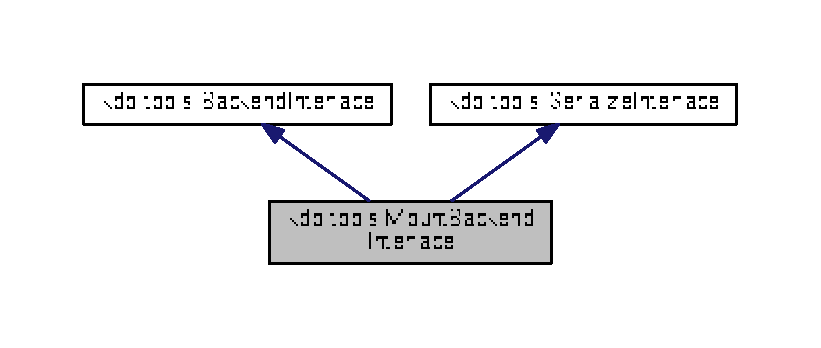
\includegraphics[width=350pt]{classkdb_1_1tools_1_1MountBackendInterface__coll__graph}
\end{center}
\end{figure}


\subsection{Detailed Description}
Interface to work with mountpoints (backends) for factory. 

The documentation for this class was generated from the following files\+:\begin{DoxyCompactItemize}
\item 
\hyperlink{backend_8hpp}{backend.\+hpp}\item 
\hyperlink{src_2backend_8cpp}{src/backend.\+cpp}\end{DoxyCompactItemize}

\hypertarget{classkdb_1_1NameIterator}{\section{kdb\-:\-:Name\-Iterator Class Reference}
\label{classkdb_1_1NameIterator}\index{kdb\-::\-Name\-Iterator@{kdb\-::\-Name\-Iterator}}
}


For C++ forward Iteration over Names.  




{\ttfamily \#include $<$key.\-hpp$>$}



Inheritance diagram for kdb\-:\-:Name\-Iterator\-:
\nopagebreak
\begin{figure}[H]
\begin{center}
\leavevmode
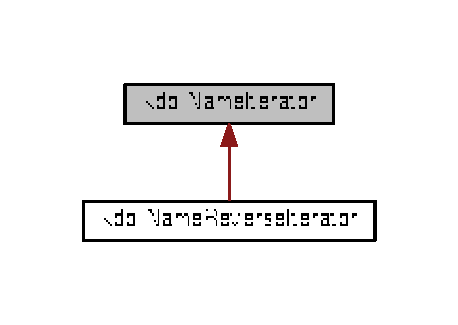
\includegraphics[width=210pt]{classkdb_1_1NameIterator__inherit__graph}
\end{center}
\end{figure}


\subsection{Detailed Description}
For C++ forward Iteration over Names. 

(External Iterator) 
\begin{DoxyCode}
\textcolor{keywordflow}{for} (std::string s:k3)
\{
   std::cout << s << std::endl;
\}
\end{DoxyCode}
 

The documentation for this class was generated from the following file\-:\begin{DoxyCompactItemize}
\item 
key.\-hpp\end{DoxyCompactItemize}

\hypertarget{classkdb_1_1NameReverseIterator}{}\doxysection{kdb\+::Name\+Reverse\+Iterator Class Reference}
\label{classkdb_1_1NameReverseIterator}\index{kdb::NameReverseIterator@{kdb::NameReverseIterator}}


For C++ reverse Iteration over Names.  




{\ttfamily \#include $<$key.\+hpp$>$}



Inheritance diagram for kdb\+::Name\+Reverse\+Iterator\+:
\nopagebreak
\begin{figure}[H]
\begin{center}
\leavevmode
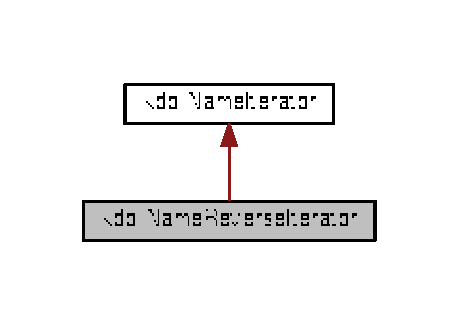
\includegraphics[width=226pt]{classkdb_1_1NameReverseIterator__inherit__graph}
\end{center}
\end{figure}


Collaboration diagram for kdb\+::Name\+Reverse\+Iterator\+:
\nopagebreak
\begin{figure}[H]
\begin{center}
\leavevmode
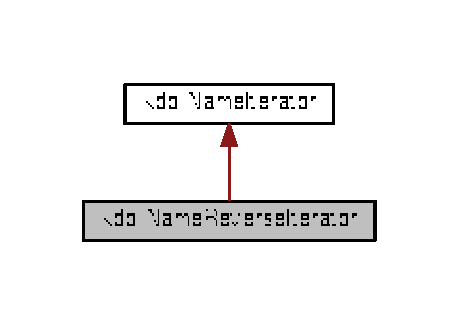
\includegraphics[width=226pt]{classkdb_1_1NameReverseIterator__coll__graph}
\end{center}
\end{figure}


\doxysubsection{Detailed Description}
For C++ reverse Iteration over Names. 

(External Iterator) 

The documentation for this class was generated from the following file\+:\begin{DoxyCompactItemize}
\item 
\mbox{\hyperlink{key_8hpp}{key.\+hpp}}\end{DoxyCompactItemize}

\hypertarget{classkdb_1_1none__t}{\section{kdb\-:\-:none\-\_\-t Class Reference}
\label{classkdb_1_1none__t}\index{kdb\-::none\-\_\-t@{kdb\-::none\-\_\-t}}
}


This type is being used as bottom type that always fails.  




{\ttfamily \#include $<$kdbvalue.\-hpp$>$}



\subsection{Detailed Description}
This type is being used as bottom type that always fails. 

The documentation for this class was generated from the following file\-:\begin{DoxyCompactItemize}
\item 
kdbvalue.\-hpp\end{DoxyCompactItemize}

\hypertarget{classkdb_1_1ObserverPolicyIs}{}\doxysection{kdb\+::Observer\+Policy\+Is$<$ Policy $>$ Class Template Reference}
\label{classkdb_1_1ObserverPolicyIs}\index{kdb::ObserverPolicyIs$<$ Policy $>$@{kdb::ObserverPolicyIs$<$ Policy $>$}}


Needed by the user to set one of the policies.  




{\ttfamily \#include $<$kdbvalue.\+hpp$>$}



Inherits kdb\+::\+Default\+Policies.



\doxysubsection{Detailed Description}
\subsubsection*{template$<$typename Policy$>$\newline
class kdb\+::\+Observer\+Policy\+Is$<$ Policy $>$}

Needed by the user to set one of the policies. 


\begin{DoxyTemplParams}{Template Parameters}
{\em Policy} & \\
\hline
\end{DoxyTemplParams}


The documentation for this class was generated from the following file\+:\begin{DoxyCompactItemize}
\item 
\mbox{\hyperlink{kdbvalue_8hpp}{kdbvalue.\+hpp}}\end{DoxyCompactItemize}

\hypertarget{structkdb_1_1PerContext}{}\section{kdb\+:\+:Per\+Context Struct Reference}
\label{structkdb_1_1PerContext}\index{kdb\+::\+Per\+Context@{kdb\+::\+Per\+Context}}


A data structure that is stored by context inside the \hyperlink{classkdb_1_1Coordinator}{Coordinator}.  




{\ttfamily \#include $<$kdbthread.\+hpp$>$}



Collaboration diagram for kdb\+:\+:Per\+Context\+:
\nopagebreak
\begin{figure}[H]
\begin{center}
\leavevmode
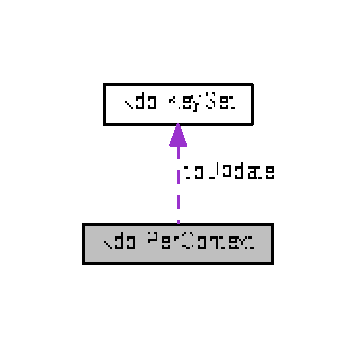
\includegraphics[width=173pt]{structkdb_1_1PerContext__coll__graph}
\end{center}
\end{figure}


\subsection{Detailed Description}
A data structure that is stored by context inside the \hyperlink{classkdb_1_1Coordinator}{Coordinator}. 

The documentation for this struct was generated from the following file\+:\begin{DoxyCompactItemize}
\item 
\hyperlink{kdbthread_8hpp}{kdbthread.\+hpp}\end{DoxyCompactItemize}

\hypertarget{classkdb_1_1tools_1_1Plugin}{\section{kdb\+:\+:tools\+:\+:Plugin Class Reference}
\label{classkdb_1_1tools_1_1Plugin}\index{kdb\+::tools\+::\+Plugin@{kdb\+::tools\+::\+Plugin}}
}


This is a C++ representation of a plugin.  




{\ttfamily \#include $<$plugin.\+hpp$>$}

\subsection*{Public Member Functions}
\begin{DoxyCompactItemize}
\item 
\hypertarget{classkdb_1_1tools_1_1Plugin_a3a0c6a956d1714002ef9baf8c9d99167}{void \hyperlink{classkdb_1_1tools_1_1Plugin_a3a0c6a956d1714002ef9baf8c9d99167}{load\+Info} ()}\label{classkdb_1_1tools_1_1Plugin_a3a0c6a956d1714002ef9baf8c9d99167}

\begin{DoxyCompactList}\small\item\em Gets the configuration for the plugin. \end{DoxyCompactList}\item 
\hypertarget{classkdb_1_1tools_1_1Plugin_adfcba2fbdeb436a1083410df804d5fb0}{void \hyperlink{classkdb_1_1tools_1_1Plugin_adfcba2fbdeb436a1083410df804d5fb0}{parse} ()}\label{classkdb_1_1tools_1_1Plugin_adfcba2fbdeb436a1083410df804d5fb0}

\begin{DoxyCompactList}\small\item\em Creates symbol and info table. \end{DoxyCompactList}\item 
void \hyperlink{classkdb_1_1tools_1_1Plugin_a5bb3db65b9d87d18787da8cc65eaca65}{check} (std\+::vector$<$ std\+::string $>$ \&warnings)
\begin{DoxyCompactList}\small\item\em Does various checks on the \hyperlink{classkdb_1_1tools_1_1Plugin}{Plugin} and throws exceptions if something is not ok. \end{DoxyCompactList}\item 
std\+::string \hyperlink{classkdb_1_1tools_1_1Plugin_a5f1dc42adda8340f330eb902812e667d}{lookup\+Info} (std\+::string item, std\+::string section=\char`\"{}infos\char`\"{})
\begin{DoxyCompactList}\small\item\em Gets the whole string of an information item. \end{DoxyCompactList}\item 
bool \hyperlink{classkdb_1_1tools_1_1Plugin_a7911f8c46aea6fe4ec6fcb4788b77beb}{find\+Info} (std\+::string \hyperlink{classkdb_1_1tools_1_1Plugin_a5bb3db65b9d87d18787da8cc65eaca65}{check}, std\+::string item, std\+::string section=\char`\"{}infos\char`\"{})
\begin{DoxyCompactList}\small\item\em Searches within a string of an information item. \end{DoxyCompactList}\item 
\hyperlink{classkdb_1_1KeySet}{kdb\+::\+Key\+Set} \hyperlink{classkdb_1_1tools_1_1Plugin_aa4eac3b2b515104a0d595c717c546ec0}{get\+Info} ()
\begin{DoxyCompactList}\small\item\em Returns the whole keyset of information. \end{DoxyCompactList}\item 
\hyperlink{classkdb_1_1KeySet}{kdb\+::\+Key\+Set} \hyperlink{classkdb_1_1tools_1_1Plugin_ad2a0a4a64d17c479e7cd8b1402275cc7}{get\+Needed\+Config} ()
\begin{DoxyCompactList}\small\item\em In the plugin's contract there is a description of which config is needed in order to work together with a backend properly. \end{DoxyCompactList}\item 
\hyperlink{classkdb_1_1KeySet}{kdb\+::\+Key\+Set} \hyperlink{classkdb_1_1tools_1_1Plugin_af3004444f5ef05dc8106646ff2b95694}{get\+Config} ()
\begin{DoxyCompactList}\small\item\em return the plugin config \end{DoxyCompactList}\item 
func\+\_\+t \hyperlink{classkdb_1_1tools_1_1Plugin_aca31140802ab463d5bddd95dee73194d}{get\+Symbol} (std\+::string which)
\begin{DoxyCompactList}\small\item\em Returns symbol to a function. \end{DoxyCompactList}\item 
int \hyperlink{classkdb_1_1tools_1_1Plugin_a680a490123b5290441d76ef2c1e3f1fa}{open} (\hyperlink{classkdb_1_1Key}{kdb\+::\+Key} \&error\+Key)
\begin{DoxyCompactList}\small\item\em Calls the open function of the plugin. \end{DoxyCompactList}\item 
int \hyperlink{classkdb_1_1tools_1_1Plugin_a40b5fd413f3f6da735680ed8d7c8a6a2}{close} (\hyperlink{classkdb_1_1Key}{kdb\+::\+Key} \&error\+Key)
\begin{DoxyCompactList}\small\item\em Calls the close function of the plugin. \end{DoxyCompactList}\item 
int \hyperlink{classkdb_1_1tools_1_1Plugin_a2aa6ff55f9cf81a59d2a8d271fe68e0f}{get} (\hyperlink{classkdb_1_1KeySet}{kdb\+::\+Key\+Set} \&ks, \hyperlink{classkdb_1_1Key}{kdb\+::\+Key} \&parent\+Key)
\begin{DoxyCompactList}\small\item\em Calls the get function of the plugin. \end{DoxyCompactList}\item 
int \hyperlink{classkdb_1_1tools_1_1Plugin_abf84d512b48f6fa1b89636217537cde0}{set} (\hyperlink{classkdb_1_1KeySet}{kdb\+::\+Key\+Set} \&ks, \hyperlink{classkdb_1_1Key}{kdb\+::\+Key} \&parent\+Key)
\begin{DoxyCompactList}\small\item\em Calls the set function of the plugin. \end{DoxyCompactList}\item 
int \hyperlink{classkdb_1_1tools_1_1Plugin_a8ec348b49a34ef17fda64cb289b8cf64}{error} (\hyperlink{classkdb_1_1KeySet}{kdb\+::\+Key\+Set} \&ks, \hyperlink{classkdb_1_1Key}{kdb\+::\+Key} \&parent\+Key)
\begin{DoxyCompactList}\small\item\em Calls the error function of the plugin. \end{DoxyCompactList}\item 
std\+::string \hyperlink{classkdb_1_1tools_1_1Plugin_ae4b82f943d0cdb0dd355924aa3201d6f}{name} ()
\item 
std\+::string \hyperlink{classkdb_1_1tools_1_1Plugin_af2fa892b6a8861419b1c1c2b3d39ed1e}{refname} ()
\end{DoxyCompactItemize}
\subsection*{Data Fields}
\begin{DoxyCompactItemize}
\item 
bool \hyperlink{classkdb_1_1tools_1_1Plugin_aee8ae2b5708c74d4ccdc1bf9e8794636}{first\+Ref}
\begin{DoxyCompactList}\small\item\em Is toggled during serialization. \end{DoxyCompactList}\end{DoxyCompactItemize}


\subsection{Detailed Description}
This is a C++ representation of a plugin. 

It will load an Elektra plugin using the module loader from Elektra.

Then you can either check the plugins configuration using \hyperlink{classkdb_1_1tools_1_1Plugin_a3a0c6a956d1714002ef9baf8c9d99167}{load\+Info()}, \hyperlink{classkdb_1_1tools_1_1Plugin_adfcba2fbdeb436a1083410df804d5fb0}{parse()} and check. Symbols can then be retrieved with \hyperlink{classkdb_1_1tools_1_1Plugin_aca31140802ab463d5bddd95dee73194d}{get\+Symbol()}.

Or you can use the normal \hyperlink{classkdb_1_1tools_1_1Plugin_a680a490123b5290441d76ef2c1e3f1fa}{open()}, \hyperlink{classkdb_1_1tools_1_1Plugin_a40b5fd413f3f6da735680ed8d7c8a6a2}{close()}, \hyperlink{classkdb_1_1tools_1_1Plugin_a2aa6ff55f9cf81a59d2a8d271fe68e0f}{get()}, \hyperlink{classkdb_1_1tools_1_1Plugin_abf84d512b48f6fa1b89636217537cde0}{set()} and \hyperlink{classkdb_1_1tools_1_1Plugin_a8ec348b49a34ef17fda64cb289b8cf64}{error()} A\+P\+I which every plugin exports. 

\subsection{Member Function Documentation}
\hypertarget{classkdb_1_1tools_1_1Plugin_a5bb3db65b9d87d18787da8cc65eaca65}{\index{kdb\+::tools\+::\+Plugin@{kdb\+::tools\+::\+Plugin}!check@{check}}
\index{check@{check}!kdb\+::tools\+::\+Plugin@{kdb\+::tools\+::\+Plugin}}
\subsubsection[{check}]{\setlength{\rightskip}{0pt plus 5cm}void kdb\+::tools\+::\+Plugin\+::check (
\begin{DoxyParamCaption}
\item[{std\+::vector$<$ std\+::string $>$ \&}]{warnings}
\end{DoxyParamCaption}
)}}\label{classkdb_1_1tools_1_1Plugin_a5bb3db65b9d87d18787da8cc65eaca65}


Does various checks on the \hyperlink{classkdb_1_1tools_1_1Plugin}{Plugin} and throws exceptions if something is not ok. 


\begin{DoxyItemize}
\item Check if \hyperlink{classkdb_1_1tools_1_1Plugin}{Plugin} is compatible to current Version of Backend-\/\+A\+P\+I.
\end{DoxyItemize}


\begin{DoxyExceptions}{Exceptions}
{\em Plugin\+Check\+Exception} & if there are errors \\
\hline
\end{DoxyExceptions}

\begin{DoxyParams}{Parameters}
{\em warnings} & for warnings\\
\hline
\end{DoxyParams}
\begin{DoxyPrecond}{Precondition}
\hyperlink{classkdb_1_1tools_1_1Plugin_adfcba2fbdeb436a1083410df804d5fb0}{parse()} 
\end{DoxyPrecond}
\hypertarget{classkdb_1_1tools_1_1Plugin_a40b5fd413f3f6da735680ed8d7c8a6a2}{\index{kdb\+::tools\+::\+Plugin@{kdb\+::tools\+::\+Plugin}!close@{close}}
\index{close@{close}!kdb\+::tools\+::\+Plugin@{kdb\+::tools\+::\+Plugin}}
\subsubsection[{close}]{\setlength{\rightskip}{0pt plus 5cm}int kdb\+::tools\+::\+Plugin\+::close (
\begin{DoxyParamCaption}
\item[{{\bf kdb\+::\+Key} \&}]{error\+Key}
\end{DoxyParamCaption}
)}}\label{classkdb_1_1tools_1_1Plugin_a40b5fd413f3f6da735680ed8d7c8a6a2}


Calls the close function of the plugin. 

\begin{DoxyPrecond}{Precondition}
\hyperlink{classkdb_1_1tools_1_1Plugin_adfcba2fbdeb436a1083410df804d5fb0}{parse()} 
\end{DoxyPrecond}
\hypertarget{classkdb_1_1tools_1_1Plugin_a8ec348b49a34ef17fda64cb289b8cf64}{\index{kdb\+::tools\+::\+Plugin@{kdb\+::tools\+::\+Plugin}!error@{error}}
\index{error@{error}!kdb\+::tools\+::\+Plugin@{kdb\+::tools\+::\+Plugin}}
\subsubsection[{error}]{\setlength{\rightskip}{0pt plus 5cm}int kdb\+::tools\+::\+Plugin\+::error (
\begin{DoxyParamCaption}
\item[{{\bf kdb\+::\+Key\+Set} \&}]{ks, }
\item[{{\bf kdb\+::\+Key} \&}]{parent\+Key}
\end{DoxyParamCaption}
)}}\label{classkdb_1_1tools_1_1Plugin_a8ec348b49a34ef17fda64cb289b8cf64}


Calls the error function of the plugin. 

\begin{DoxyPrecond}{Precondition}
\hyperlink{classkdb_1_1tools_1_1Plugin_adfcba2fbdeb436a1083410df804d5fb0}{parse()} 
\end{DoxyPrecond}
\hypertarget{classkdb_1_1tools_1_1Plugin_a7911f8c46aea6fe4ec6fcb4788b77beb}{\index{kdb\+::tools\+::\+Plugin@{kdb\+::tools\+::\+Plugin}!find\+Info@{find\+Info}}
\index{find\+Info@{find\+Info}!kdb\+::tools\+::\+Plugin@{kdb\+::tools\+::\+Plugin}}
\subsubsection[{find\+Info}]{\setlength{\rightskip}{0pt plus 5cm}bool kdb\+::tools\+::\+Plugin\+::find\+Info (
\begin{DoxyParamCaption}
\item[{std\+::string}]{check, }
\item[{std\+::string}]{item, }
\item[{std\+::string}]{section = {\ttfamily \char`\"{}infos\char`\"{}}}
\end{DoxyParamCaption}
)}}\label{classkdb_1_1tools_1_1Plugin_a7911f8c46aea6fe4ec6fcb4788b77beb}


Searches within a string of an information item. 

\begin{DoxyPrecond}{Precondition}
\hyperlink{classkdb_1_1tools_1_1Plugin_a3a0c6a956d1714002ef9baf8c9d99167}{load\+Info()} 
\end{DoxyPrecond}
\hypertarget{classkdb_1_1tools_1_1Plugin_a2aa6ff55f9cf81a59d2a8d271fe68e0f}{\index{kdb\+::tools\+::\+Plugin@{kdb\+::tools\+::\+Plugin}!get@{get}}
\index{get@{get}!kdb\+::tools\+::\+Plugin@{kdb\+::tools\+::\+Plugin}}
\subsubsection[{get}]{\setlength{\rightskip}{0pt plus 5cm}int kdb\+::tools\+::\+Plugin\+::get (
\begin{DoxyParamCaption}
\item[{{\bf kdb\+::\+Key\+Set} \&}]{ks, }
\item[{{\bf kdb\+::\+Key} \&}]{parent\+Key}
\end{DoxyParamCaption}
)}}\label{classkdb_1_1tools_1_1Plugin_a2aa6ff55f9cf81a59d2a8d271fe68e0f}


Calls the get function of the plugin. 

\begin{DoxyPrecond}{Precondition}
\hyperlink{classkdb_1_1tools_1_1Plugin_adfcba2fbdeb436a1083410df804d5fb0}{parse()} 
\end{DoxyPrecond}
\hypertarget{classkdb_1_1tools_1_1Plugin_af3004444f5ef05dc8106646ff2b95694}{\index{kdb\+::tools\+::\+Plugin@{kdb\+::tools\+::\+Plugin}!get\+Config@{get\+Config}}
\index{get\+Config@{get\+Config}!kdb\+::tools\+::\+Plugin@{kdb\+::tools\+::\+Plugin}}
\subsubsection[{get\+Config}]{\setlength{\rightskip}{0pt plus 5cm}{\bf kdb\+::\+Key\+Set} kdb\+::tools\+::\+Plugin\+::get\+Config (
\begin{DoxyParamCaption}
{}
\end{DoxyParamCaption}
)}}\label{classkdb_1_1tools_1_1Plugin_af3004444f5ef05dc8106646ff2b95694}


return the plugin config 

\begin{DoxyReturn}{Returns}
the config supplied with constructor 
\end{DoxyReturn}
\begin{DoxySeeAlso}{See also}
\hyperlink{classkdb_1_1tools_1_1Plugin_ad2a0a4a64d17c479e7cd8b1402275cc7}{get\+Needed\+Config()} 
\end{DoxySeeAlso}
\hypertarget{classkdb_1_1tools_1_1Plugin_aa4eac3b2b515104a0d595c717c546ec0}{\index{kdb\+::tools\+::\+Plugin@{kdb\+::tools\+::\+Plugin}!get\+Info@{get\+Info}}
\index{get\+Info@{get\+Info}!kdb\+::tools\+::\+Plugin@{kdb\+::tools\+::\+Plugin}}
\subsubsection[{get\+Info}]{\setlength{\rightskip}{0pt plus 5cm}{\bf kdb\+::\+Key\+Set} kdb\+::tools\+::\+Plugin\+::get\+Info (
\begin{DoxyParamCaption}
{}
\end{DoxyParamCaption}
)\hspace{0.3cm}{\ttfamily [inline]}}}\label{classkdb_1_1tools_1_1Plugin_aa4eac3b2b515104a0d595c717c546ec0}


Returns the whole keyset of information. 

\begin{DoxyPrecond}{Precondition}
\hyperlink{classkdb_1_1tools_1_1Plugin_a3a0c6a956d1714002ef9baf8c9d99167}{load\+Info()} 
\end{DoxyPrecond}
\hypertarget{classkdb_1_1tools_1_1Plugin_ad2a0a4a64d17c479e7cd8b1402275cc7}{\index{kdb\+::tools\+::\+Plugin@{kdb\+::tools\+::\+Plugin}!get\+Needed\+Config@{get\+Needed\+Config}}
\index{get\+Needed\+Config@{get\+Needed\+Config}!kdb\+::tools\+::\+Plugin@{kdb\+::tools\+::\+Plugin}}
\subsubsection[{get\+Needed\+Config}]{\setlength{\rightskip}{0pt plus 5cm}{\bf kdb\+::\+Key\+Set} kdb\+::tools\+::\+Plugin\+::get\+Needed\+Config (
\begin{DoxyParamCaption}
{}
\end{DoxyParamCaption}
)}}\label{classkdb_1_1tools_1_1Plugin_ad2a0a4a64d17c479e7cd8b1402275cc7}


In the plugin's contract there is a description of which config is needed in order to work together with a backend properly. 

\begin{DoxyReturn}{Returns}
the keyset with the config needed for the backend. 
\end{DoxyReturn}
\begin{DoxySeeAlso}{See also}
\hyperlink{classkdb_1_1tools_1_1Plugin_af3004444f5ef05dc8106646ff2b95694}{get\+Config()} 
\end{DoxySeeAlso}
\begin{DoxyPrecond}{Precondition}
\hyperlink{classkdb_1_1tools_1_1Plugin_a3a0c6a956d1714002ef9baf8c9d99167}{load\+Info()} 
\end{DoxyPrecond}
\hypertarget{classkdb_1_1tools_1_1Plugin_aca31140802ab463d5bddd95dee73194d}{\index{kdb\+::tools\+::\+Plugin@{kdb\+::tools\+::\+Plugin}!get\+Symbol@{get\+Symbol}}
\index{get\+Symbol@{get\+Symbol}!kdb\+::tools\+::\+Plugin@{kdb\+::tools\+::\+Plugin}}
\subsubsection[{get\+Symbol}]{\setlength{\rightskip}{0pt plus 5cm}func\+\_\+t kdb\+::tools\+::\+Plugin\+::get\+Symbol (
\begin{DoxyParamCaption}
\item[{std\+::string}]{which}
\end{DoxyParamCaption}
)\hspace{0.3cm}{\ttfamily [inline]}}}\label{classkdb_1_1tools_1_1Plugin_aca31140802ab463d5bddd95dee73194d}


Returns symbol to a function. 

\begin{DoxyPrecond}{Precondition}
\hyperlink{classkdb_1_1tools_1_1Plugin_adfcba2fbdeb436a1083410df804d5fb0}{parse()} 
\end{DoxyPrecond}
\hypertarget{classkdb_1_1tools_1_1Plugin_a5f1dc42adda8340f330eb902812e667d}{\index{kdb\+::tools\+::\+Plugin@{kdb\+::tools\+::\+Plugin}!lookup\+Info@{lookup\+Info}}
\index{lookup\+Info@{lookup\+Info}!kdb\+::tools\+::\+Plugin@{kdb\+::tools\+::\+Plugin}}
\subsubsection[{lookup\+Info}]{\setlength{\rightskip}{0pt plus 5cm}std\+::string kdb\+::tools\+::\+Plugin\+::lookup\+Info (
\begin{DoxyParamCaption}
\item[{std\+::string}]{item, }
\item[{std\+::string}]{section = {\ttfamily \char`\"{}infos\char`\"{}}}
\end{DoxyParamCaption}
)}}\label{classkdb_1_1tools_1_1Plugin_a5f1dc42adda8340f330eb902812e667d}


Gets the whole string of an information item. 

\begin{DoxyPrecond}{Precondition}
\hyperlink{classkdb_1_1tools_1_1Plugin_a3a0c6a956d1714002ef9baf8c9d99167}{load\+Info()} 
\end{DoxyPrecond}
\hypertarget{classkdb_1_1tools_1_1Plugin_ae4b82f943d0cdb0dd355924aa3201d6f}{\index{kdb\+::tools\+::\+Plugin@{kdb\+::tools\+::\+Plugin}!name@{name}}
\index{name@{name}!kdb\+::tools\+::\+Plugin@{kdb\+::tools\+::\+Plugin}}
\subsubsection[{name}]{\setlength{\rightskip}{0pt plus 5cm}std\+::string kdb\+::tools\+::\+Plugin\+::name (
\begin{DoxyParamCaption}
{}
\end{DoxyParamCaption}
)}}\label{classkdb_1_1tools_1_1Plugin_ae4b82f943d0cdb0dd355924aa3201d6f}
\begin{DoxyReturn}{Returns}
the name of the plugin 
\end{DoxyReturn}
\hypertarget{classkdb_1_1tools_1_1Plugin_a680a490123b5290441d76ef2c1e3f1fa}{\index{kdb\+::tools\+::\+Plugin@{kdb\+::tools\+::\+Plugin}!open@{open}}
\index{open@{open}!kdb\+::tools\+::\+Plugin@{kdb\+::tools\+::\+Plugin}}
\subsubsection[{open}]{\setlength{\rightskip}{0pt plus 5cm}int kdb\+::tools\+::\+Plugin\+::open (
\begin{DoxyParamCaption}
\item[{{\bf kdb\+::\+Key} \&}]{error\+Key}
\end{DoxyParamCaption}
)}}\label{classkdb_1_1tools_1_1Plugin_a680a490123b5290441d76ef2c1e3f1fa}


Calls the open function of the plugin. 

\begin{DoxyPrecond}{Precondition}
\hyperlink{classkdb_1_1tools_1_1Plugin_adfcba2fbdeb436a1083410df804d5fb0}{parse()} 
\end{DoxyPrecond}
\hypertarget{classkdb_1_1tools_1_1Plugin_af2fa892b6a8861419b1c1c2b3d39ed1e}{\index{kdb\+::tools\+::\+Plugin@{kdb\+::tools\+::\+Plugin}!refname@{refname}}
\index{refname@{refname}!kdb\+::tools\+::\+Plugin@{kdb\+::tools\+::\+Plugin}}
\subsubsection[{refname}]{\setlength{\rightskip}{0pt plus 5cm}std\+::string kdb\+::tools\+::\+Plugin\+::refname (
\begin{DoxyParamCaption}
{}
\end{DoxyParamCaption}
)}}\label{classkdb_1_1tools_1_1Plugin_af2fa892b6a8861419b1c1c2b3d39ed1e}
\begin{DoxyReturn}{Returns}
the name how it would be referred to in mountpoint 
\end{DoxyReturn}
\hypertarget{classkdb_1_1tools_1_1Plugin_abf84d512b48f6fa1b89636217537cde0}{\index{kdb\+::tools\+::\+Plugin@{kdb\+::tools\+::\+Plugin}!set@{set}}
\index{set@{set}!kdb\+::tools\+::\+Plugin@{kdb\+::tools\+::\+Plugin}}
\subsubsection[{set}]{\setlength{\rightskip}{0pt plus 5cm}int kdb\+::tools\+::\+Plugin\+::set (
\begin{DoxyParamCaption}
\item[{{\bf kdb\+::\+Key\+Set} \&}]{ks, }
\item[{{\bf kdb\+::\+Key} \&}]{parent\+Key}
\end{DoxyParamCaption}
)}}\label{classkdb_1_1tools_1_1Plugin_abf84d512b48f6fa1b89636217537cde0}


Calls the set function of the plugin. 

\begin{DoxyPrecond}{Precondition}
\hyperlink{classkdb_1_1tools_1_1Plugin_adfcba2fbdeb436a1083410df804d5fb0}{parse()} 
\end{DoxyPrecond}


\subsection{Field Documentation}
\hypertarget{classkdb_1_1tools_1_1Plugin_aee8ae2b5708c74d4ccdc1bf9e8794636}{\index{kdb\+::tools\+::\+Plugin@{kdb\+::tools\+::\+Plugin}!first\+Ref@{first\+Ref}}
\index{first\+Ref@{first\+Ref}!kdb\+::tools\+::\+Plugin@{kdb\+::tools\+::\+Plugin}}
\subsubsection[{first\+Ref}]{\setlength{\rightskip}{0pt plus 5cm}bool kdb\+::tools\+::\+Plugin\+::first\+Ref}}\label{classkdb_1_1tools_1_1Plugin_aee8ae2b5708c74d4ccdc1bf9e8794636}


Is toggled during serialization. 

(is a hack, only allows a single serialization!) 

The documentation for this class was generated from the following files\+:\begin{DoxyCompactItemize}
\item 
\hyperlink{plugin_8hpp}{plugin.\+hpp}\item 
\hyperlink{plugin_8cpp}{plugin.\+cpp}\end{DoxyCompactItemize}

\hypertarget{classkdb_1_1tools_1_1PluginAdder}{}\section{kdb\+:\+:tools\+:\+:Plugin\+Adder Class Reference}
\label{classkdb_1_1tools_1_1PluginAdder}\index{kdb\+::tools\+::\+Plugin\+Adder@{kdb\+::tools\+::\+Plugin\+Adder}}


Adds plugins in a generic map.  




{\ttfamily \#include $<$backend.\+hpp$>$}



Inheritance diagram for kdb\+:\+:tools\+:\+:Plugin\+Adder\+:
\nopagebreak
\begin{figure}[H]
\begin{center}
\leavevmode
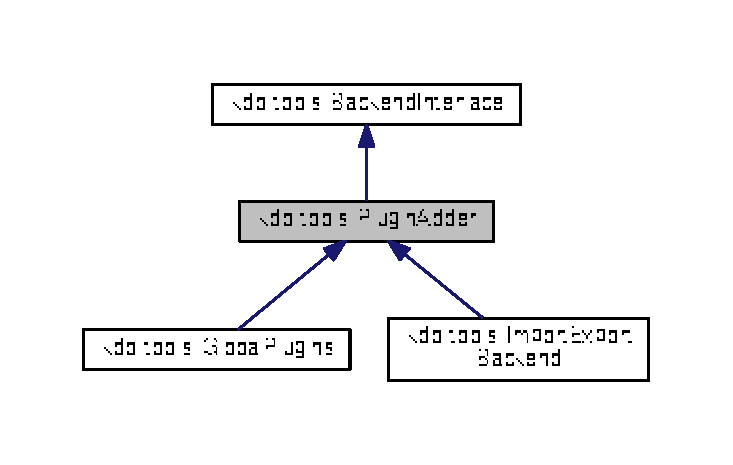
\includegraphics[width=346pt]{classkdb_1_1tools_1_1PluginAdder__inherit__graph}
\end{center}
\end{figure}


Collaboration diagram for kdb\+:\+:tools\+:\+:Plugin\+Adder\+:
\nopagebreak
\begin{figure}[H]
\begin{center}
\leavevmode
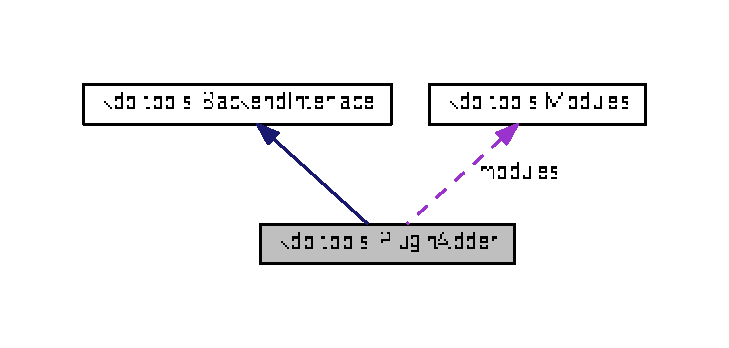
\includegraphics[width=342pt]{classkdb_1_1tools_1_1PluginAdder__coll__graph}
\end{center}
\end{figure}


\subsection{Detailed Description}
Adds plugins in a generic map. 

The documentation for this class was generated from the following files\+:\begin{DoxyCompactItemize}
\item 
\hyperlink{backend_8hpp}{backend.\+hpp}\item 
\hyperlink{src_2backend_8cpp}{src/backend.\+cpp}\end{DoxyCompactItemize}

\hypertarget{classkdb_1_1tools_1_1PluginDatabase}{}\doxysection{kdb\+::tools\+::Plugin\+Database Class Reference}
\label{classkdb_1_1tools_1_1PluginDatabase}\index{kdb::tools::PluginDatabase@{kdb::tools::PluginDatabase}}


Loads all plugins and allows us to query them.  




{\ttfamily \#include $<$plugindatabase.\+hpp$>$}



Inheritance diagram for kdb\+::tools\+::Plugin\+Database\+:
\nopagebreak
\begin{figure}[H]
\begin{center}
\leavevmode
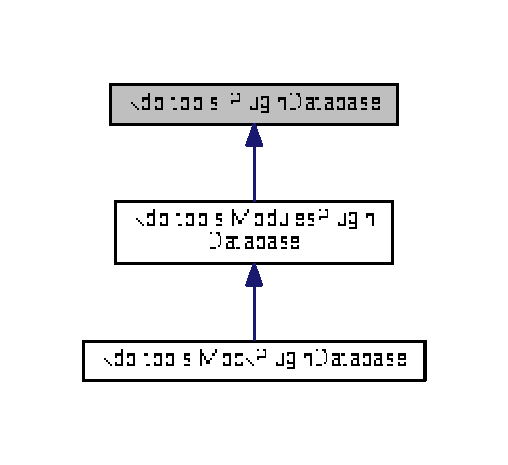
\includegraphics[width=253pt]{classkdb_1_1tools_1_1PluginDatabase__inherit__graph}
\end{center}
\end{figure}
\doxysubsection*{Public Types}
\begin{DoxyCompactItemize}
\item 
enum \mbox{\hyperlink{classkdb_1_1tools_1_1PluginDatabase_afc91ff760616ee83c6afb70e5a2f0601}{Status}} \{ \mbox{\hyperlink{classkdb_1_1tools_1_1PluginDatabase_afc91ff760616ee83c6afb70e5a2f0601a73ff10d6a07213c277db4326b3df6c4b}{provides}}, 
\mbox{\hyperlink{classkdb_1_1tools_1_1PluginDatabase_afc91ff760616ee83c6afb70e5a2f0601a2b7279a50ed80231a60b0435340c31a8}{real}}, 
\mbox{\hyperlink{classkdb_1_1tools_1_1PluginDatabase_afc91ff760616ee83c6afb70e5a2f0601ae789aaff1847ebb77eecb027c5ee0401}{missing}}
 \}
\end{DoxyCompactItemize}
\doxysubsection*{Public Member Functions}
\begin{DoxyCompactItemize}
\item 
virtual std\+::vector$<$ std\+::string $>$ \mbox{\hyperlink{classkdb_1_1tools_1_1PluginDatabase_adc1f43ccefdd7fc15a57db7571420642}{list\+All\+Plugins}} () const =0
\begin{DoxyCompactList}\small\item\em list all plugins \end{DoxyCompactList}\item 
virtual std\+::string \mbox{\hyperlink{classkdb_1_1tools_1_1PluginDatabase_ac0af2ec31a98f4176c19eaf34977abbe}{lookup\+Info}} (\mbox{\hyperlink{classkdb_1_1tools_1_1PluginSpec}{Plugin\+Spec}} const \&whichplugin, std\+::string const \&which) const =0
\begin{DoxyCompactList}\small\item\em lookup contract clauses or dynamic information \end{DoxyCompactList}\item 
virtual func\+\_\+t \mbox{\hyperlink{classkdb_1_1tools_1_1PluginDatabase_a87b5ef6ee66ce1ad46cc590a2b60b9fa}{get\+Symbol}} (\mbox{\hyperlink{classkdb_1_1tools_1_1PluginSpec}{Plugin\+Spec}} const \&whichplugin, std\+::string const \&which) const =0
\begin{DoxyCompactList}\small\item\em get exported plugin symbol \end{DoxyCompactList}\item 
virtual \mbox{\hyperlink{classkdb_1_1tools_1_1PluginSpec}{Plugin\+Spec}} \mbox{\hyperlink{classkdb_1_1tools_1_1PluginDatabase_a03a416f66d6525f46929e5a68d9db3f7}{lookup\+Metadata}} (std\+::string const \&which) const =0
\begin{DoxyCompactList}\small\item\em lookup which plugin handles metadata \end{DoxyCompactList}\item 
virtual \mbox{\hyperlink{classkdb_1_1tools_1_1PluginSpec}{Plugin\+Spec}} \mbox{\hyperlink{classkdb_1_1tools_1_1PluginDatabase_a43abe56a024218ecee48526ced699f05}{lookup\+Provides}} (std\+::string const \&\mbox{\hyperlink{classkdb_1_1tools_1_1PluginDatabase_afc91ff760616ee83c6afb70e5a2f0601a73ff10d6a07213c277db4326b3df6c4b}{provides}}) const =0
\begin{DoxyCompactList}\small\item\em lookup which plugin is a provider for that plugin \end{DoxyCompactList}\item 
virtual std\+::map$<$ int, \mbox{\hyperlink{classkdb_1_1tools_1_1PluginSpec}{Plugin\+Spec}} $>$ \mbox{\hyperlink{classkdb_1_1tools_1_1PluginDatabase_aa918b547973f627a5604fa3b2b3faf30}{lookup\+All\+Provides\+With\+Status}} (std\+::string const \&\mbox{\hyperlink{classkdb_1_1tools_1_1PluginDatabase_afc91ff760616ee83c6afb70e5a2f0601a73ff10d6a07213c277db4326b3df6c4b}{provides}}) const =0
\begin{DoxyCompactList}\small\item\em looks up all plugins which are a suitable provider \end{DoxyCompactList}\item 
virtual std\+::vector$<$ \mbox{\hyperlink{classkdb_1_1tools_1_1PluginSpec}{Plugin\+Spec}} $>$ \mbox{\hyperlink{classkdb_1_1tools_1_1PluginDatabase_a3ed261ad8562c423b64cf34cbc086161}{lookup\+All\+Provides}} (std\+::string const \&\mbox{\hyperlink{classkdb_1_1tools_1_1PluginDatabase_afc91ff760616ee83c6afb70e5a2f0601a73ff10d6a07213c277db4326b3df6c4b}{provides}}) const =0
\begin{DoxyCompactList}\small\item\em looks up all plugins which are a suitable provider \end{DoxyCompactList}\end{DoxyCompactItemize}
\doxysubsection*{Static Public Member Functions}
\begin{DoxyCompactItemize}
\item 
static int \mbox{\hyperlink{classkdb_1_1tools_1_1PluginDatabase_ab901b98a6c7661bbccffa8ab9ff62dc6}{calculate\+Status}} (std\+::string status\+String)
\end{DoxyCompactItemize}


\doxysubsection{Detailed Description}
Loads all plugins and allows us to query them. 

\doxysubsection{Member Enumeration Documentation}
\mbox{\Hypertarget{classkdb_1_1tools_1_1PluginDatabase_afc91ff760616ee83c6afb70e5a2f0601}\label{classkdb_1_1tools_1_1PluginDatabase_afc91ff760616ee83c6afb70e5a2f0601}} 
\index{kdb::tools::PluginDatabase@{kdb::tools::PluginDatabase}!Status@{Status}}
\index{Status@{Status}!kdb::tools::PluginDatabase@{kdb::tools::PluginDatabase}}
\doxysubsubsection{\texorpdfstring{Status}{Status}}
{\footnotesize\ttfamily enum \mbox{\hyperlink{classkdb_1_1tools_1_1PluginDatabase_afc91ff760616ee83c6afb70e5a2f0601}{kdb\+::tools\+::\+Plugin\+Database\+::\+Status}}}

\begin{DoxyEnumFields}{Enumerator}
\raisebox{\heightof{T}}[0pt][0pt]{\index{provides@{provides}!kdb::tools::PluginDatabase@{kdb::tools::PluginDatabase}}\index{kdb::tools::PluginDatabase@{kdb::tools::PluginDatabase}!provides@{provides}}}\mbox{\Hypertarget{classkdb_1_1tools_1_1PluginDatabase_afc91ff760616ee83c6afb70e5a2f0601a73ff10d6a07213c277db4326b3df6c4b}\label{classkdb_1_1tools_1_1PluginDatabase_afc91ff760616ee83c6afb70e5a2f0601a73ff10d6a07213c277db4326b3df6c4b}} 
provides&does not directly, but can be loaded via provides \\
\hline

\raisebox{\heightof{T}}[0pt][0pt]{\index{real@{real}!kdb::tools::PluginDatabase@{kdb::tools::PluginDatabase}}\index{kdb::tools::PluginDatabase@{kdb::tools::PluginDatabase}!real@{real}}}\mbox{\Hypertarget{classkdb_1_1tools_1_1PluginDatabase_afc91ff760616ee83c6afb70e5a2f0601a2b7279a50ed80231a60b0435340c31a8}\label{classkdb_1_1tools_1_1PluginDatabase_afc91ff760616ee83c6afb70e5a2f0601a2b7279a50ed80231a60b0435340c31a8}} 
real&exists and working as given \\
\hline

\raisebox{\heightof{T}}[0pt][0pt]{\index{missing@{missing}!kdb::tools::PluginDatabase@{kdb::tools::PluginDatabase}}\index{kdb::tools::PluginDatabase@{kdb::tools::PluginDatabase}!missing@{missing}}}\mbox{\Hypertarget{classkdb_1_1tools_1_1PluginDatabase_afc91ff760616ee83c6afb70e5a2f0601ae789aaff1847ebb77eecb027c5ee0401}\label{classkdb_1_1tools_1_1PluginDatabase_afc91ff760616ee83c6afb70e5a2f0601ae789aaff1847ebb77eecb027c5ee0401}} 
missing&does not exist or cannot be loaded \\
\hline

\end{DoxyEnumFields}


\doxysubsection{Member Function Documentation}
\mbox{\Hypertarget{classkdb_1_1tools_1_1PluginDatabase_ab901b98a6c7661bbccffa8ab9ff62dc6}\label{classkdb_1_1tools_1_1PluginDatabase_ab901b98a6c7661bbccffa8ab9ff62dc6}} 
\index{kdb::tools::PluginDatabase@{kdb::tools::PluginDatabase}!calculateStatus@{calculateStatus}}
\index{calculateStatus@{calculateStatus}!kdb::tools::PluginDatabase@{kdb::tools::PluginDatabase}}
\doxysubsubsection{\texorpdfstring{calculateStatus()}{calculateStatus()}}
{\footnotesize\ttfamily int kdb\+::tools\+::\+Plugin\+Database\+::calculate\+Status (\begin{DoxyParamCaption}\item[{std\+::string}]{status\+String }\end{DoxyParamCaption})\hspace{0.3cm}{\ttfamily [static]}}


\begin{DoxyParams}{Parameters}
{\em status\+String} & the string encoding the status\\
\hline
\end{DoxyParams}
\begin{DoxyReturn}{Returns}
The representing number for a given status. 
\end{DoxyReturn}
\mbox{\Hypertarget{classkdb_1_1tools_1_1PluginDatabase_a87b5ef6ee66ce1ad46cc590a2b60b9fa}\label{classkdb_1_1tools_1_1PluginDatabase_a87b5ef6ee66ce1ad46cc590a2b60b9fa}} 
\index{kdb::tools::PluginDatabase@{kdb::tools::PluginDatabase}!getSymbol@{getSymbol}}
\index{getSymbol@{getSymbol}!kdb::tools::PluginDatabase@{kdb::tools::PluginDatabase}}
\doxysubsubsection{\texorpdfstring{getSymbol()}{getSymbol()}}
{\footnotesize\ttfamily virtual func\+\_\+t kdb\+::tools\+::\+Plugin\+Database\+::get\+Symbol (\begin{DoxyParamCaption}\item[{\mbox{\hyperlink{classkdb_1_1tools_1_1PluginSpec}{Plugin\+Spec}} const \&}]{whichplugin,  }\item[{std\+::string const \&}]{which }\end{DoxyParamCaption}) const\hspace{0.3cm}{\ttfamily [pure virtual]}}



get exported plugin symbol 


\begin{DoxyParams}{Parameters}
{\em whichplugin} & from which plugin? \\
\hline
{\em which} & which symbol would you like to look up?\\
\hline
\end{DoxyParams}
\begin{DoxyReturn}{Returns}
the function pointer to the exported symbol or N\+U\+LL if the symbol was not found 
\end{DoxyReturn}


Implemented in \mbox{\hyperlink{classkdb_1_1tools_1_1MockPluginDatabase_a5a701fd310be0e9f7d14a865c0226517}{kdb\+::tools\+::\+Mock\+Plugin\+Database}}, and \mbox{\hyperlink{classkdb_1_1tools_1_1ModulesPluginDatabase_a0e81e1b7b296a52f8040fd966b461c3a}{kdb\+::tools\+::\+Modules\+Plugin\+Database}}.

\mbox{\Hypertarget{classkdb_1_1tools_1_1PluginDatabase_adc1f43ccefdd7fc15a57db7571420642}\label{classkdb_1_1tools_1_1PluginDatabase_adc1f43ccefdd7fc15a57db7571420642}} 
\index{kdb::tools::PluginDatabase@{kdb::tools::PluginDatabase}!listAllPlugins@{listAllPlugins}}
\index{listAllPlugins@{listAllPlugins}!kdb::tools::PluginDatabase@{kdb::tools::PluginDatabase}}
\doxysubsubsection{\texorpdfstring{listAllPlugins()}{listAllPlugins()}}
{\footnotesize\ttfamily virtual std\+::vector$<$std\+::string$>$ kdb\+::tools\+::\+Plugin\+Database\+::list\+All\+Plugins (\begin{DoxyParamCaption}{ }\end{DoxyParamCaption}) const\hspace{0.3cm}{\ttfamily [pure virtual]}}



list all plugins 

If Elektra is compiled with plugins, it will search for shared libraries. In any case, if no shared libraries were found it will fallback to an internal list (plugins that were compiled together with Elektra).

\begin{DoxyReturn}{Returns}
a list of all available plugins 
\end{DoxyReturn}


Implemented in \mbox{\hyperlink{classkdb_1_1tools_1_1MockPluginDatabase_a3663848683953bfad7123c48c00ab404}{kdb\+::tools\+::\+Mock\+Plugin\+Database}}, and \mbox{\hyperlink{classkdb_1_1tools_1_1ModulesPluginDatabase_a3fa5a08caf47cb79f9889641a96f197b}{kdb\+::tools\+::\+Modules\+Plugin\+Database}}.

\mbox{\Hypertarget{classkdb_1_1tools_1_1PluginDatabase_a3ed261ad8562c423b64cf34cbc086161}\label{classkdb_1_1tools_1_1PluginDatabase_a3ed261ad8562c423b64cf34cbc086161}} 
\index{kdb::tools::PluginDatabase@{kdb::tools::PluginDatabase}!lookupAllProvides@{lookupAllProvides}}
\index{lookupAllProvides@{lookupAllProvides}!kdb::tools::PluginDatabase@{kdb::tools::PluginDatabase}}
\doxysubsubsection{\texorpdfstring{lookupAllProvides()}{lookupAllProvides()}}
{\footnotesize\ttfamily virtual std\+::vector$<$\mbox{\hyperlink{classkdb_1_1tools_1_1PluginSpec}{Plugin\+Spec}}$>$ kdb\+::tools\+::\+Plugin\+Database\+::lookup\+All\+Provides (\begin{DoxyParamCaption}\item[{std\+::string const \&}]{provides }\end{DoxyParamCaption}) const\hspace{0.3cm}{\ttfamily [pure virtual]}}



looks up all plugins which are a suitable provider 

\begin{DoxyNote}{Note}
in case a plugin name is provided, the plugin with the name will also be part of the result. But if there are other plugins providing the requirement, then they will also be part of the result. The ordering of the resulting vector has no special meaning.
\end{DoxyNote}

\begin{DoxyParams}{Parameters}
{\em provides} & is the provider to find\\
\hline
\end{DoxyParams}
\begin{DoxyReturn}{Returns}
a vector of plugins offering the requirement or are named after it 
\end{DoxyReturn}


Implemented in \mbox{\hyperlink{classkdb_1_1tools_1_1ModulesPluginDatabase_a306384e88f9cf2874f6ba9ce28973a26}{kdb\+::tools\+::\+Modules\+Plugin\+Database}}.

\mbox{\Hypertarget{classkdb_1_1tools_1_1PluginDatabase_aa918b547973f627a5604fa3b2b3faf30}\label{classkdb_1_1tools_1_1PluginDatabase_aa918b547973f627a5604fa3b2b3faf30}} 
\index{kdb::tools::PluginDatabase@{kdb::tools::PluginDatabase}!lookupAllProvidesWithStatus@{lookupAllProvidesWithStatus}}
\index{lookupAllProvidesWithStatus@{lookupAllProvidesWithStatus}!kdb::tools::PluginDatabase@{kdb::tools::PluginDatabase}}
\doxysubsubsection{\texorpdfstring{lookupAllProvidesWithStatus()}{lookupAllProvidesWithStatus()}}
{\footnotesize\ttfamily virtual std\+::map$<$int, \mbox{\hyperlink{classkdb_1_1tools_1_1PluginSpec}{Plugin\+Spec}}$>$ kdb\+::tools\+::\+Plugin\+Database\+::lookup\+All\+Provides\+With\+Status (\begin{DoxyParamCaption}\item[{std\+::string const \&}]{provides }\end{DoxyParamCaption}) const\hspace{0.3cm}{\ttfamily [pure virtual]}}



looks up all plugins which are a suitable provider 

\begin{DoxyNote}{Note}
in case a plugin name is provided, the plugin with the name will also be part of the result. But if there are other plugins providing the requirement, then they will also be part of the result.
\end{DoxyNote}

\begin{DoxyParams}{Parameters}
{\em provides} & is the provider to find\\
\hline
\end{DoxyParams}
\begin{DoxyReturn}{Returns}
a map of plugins with their status offering the requirement or are named after it 
\end{DoxyReturn}


Implemented in \mbox{\hyperlink{classkdb_1_1tools_1_1ModulesPluginDatabase_abe19487ff2a2e0548288dfa2a5678ae1}{kdb\+::tools\+::\+Modules\+Plugin\+Database}}.

\mbox{\Hypertarget{classkdb_1_1tools_1_1PluginDatabase_ac0af2ec31a98f4176c19eaf34977abbe}\label{classkdb_1_1tools_1_1PluginDatabase_ac0af2ec31a98f4176c19eaf34977abbe}} 
\index{kdb::tools::PluginDatabase@{kdb::tools::PluginDatabase}!lookupInfo@{lookupInfo}}
\index{lookupInfo@{lookupInfo}!kdb::tools::PluginDatabase@{kdb::tools::PluginDatabase}}
\doxysubsubsection{\texorpdfstring{lookupInfo()}{lookupInfo()}}
{\footnotesize\ttfamily virtual std\+::string kdb\+::tools\+::\+Plugin\+Database\+::lookup\+Info (\begin{DoxyParamCaption}\item[{\mbox{\hyperlink{classkdb_1_1tools_1_1PluginSpec}{Plugin\+Spec}} const \&}]{whichplugin,  }\item[{std\+::string const \&}]{which }\end{DoxyParamCaption}) const\hspace{0.3cm}{\ttfamily [pure virtual]}}



lookup contract clauses or dynamic information 


\begin{DoxyParams}{Parameters}
{\em whichplugin} & about which plugin? \\
\hline
{\em which} & about which clause in the contract?\\
\hline
\end{DoxyParams}
\begin{DoxyReturn}{Returns}
the clause of the contract 
\end{DoxyReturn}


Implemented in \mbox{\hyperlink{classkdb_1_1tools_1_1MockPluginDatabase_ae352c27aa51bc8c2ea8c708d14f6fc76}{kdb\+::tools\+::\+Mock\+Plugin\+Database}}, and \mbox{\hyperlink{classkdb_1_1tools_1_1ModulesPluginDatabase_a3f51beee8aecb4371e7d12e98958f875}{kdb\+::tools\+::\+Modules\+Plugin\+Database}}.

\mbox{\Hypertarget{classkdb_1_1tools_1_1PluginDatabase_a03a416f66d6525f46929e5a68d9db3f7}\label{classkdb_1_1tools_1_1PluginDatabase_a03a416f66d6525f46929e5a68d9db3f7}} 
\index{kdb::tools::PluginDatabase@{kdb::tools::PluginDatabase}!lookupMetadata@{lookupMetadata}}
\index{lookupMetadata@{lookupMetadata}!kdb::tools::PluginDatabase@{kdb::tools::PluginDatabase}}
\doxysubsubsection{\texorpdfstring{lookupMetadata()}{lookupMetadata()}}
{\footnotesize\ttfamily virtual \mbox{\hyperlink{classkdb_1_1tools_1_1PluginSpec}{Plugin\+Spec}} kdb\+::tools\+::\+Plugin\+Database\+::lookup\+Metadata (\begin{DoxyParamCaption}\item[{std\+::string const \&}]{which }\end{DoxyParamCaption}) const\hspace{0.3cm}{\ttfamily [pure virtual]}}



lookup which plugin handles metadata 


\begin{DoxyParams}{Parameters}
{\em which} & the metadata of interest\\
\hline
\end{DoxyParams}
\begin{DoxyReturn}{Returns}
the best suited plugin specification which provides it 
\end{DoxyReturn}


Implemented in \mbox{\hyperlink{classkdb_1_1tools_1_1ModulesPluginDatabase_aa7f244f0271ea9b2a3f5b52779167f55}{kdb\+::tools\+::\+Modules\+Plugin\+Database}}.

\mbox{\Hypertarget{classkdb_1_1tools_1_1PluginDatabase_a43abe56a024218ecee48526ced699f05}\label{classkdb_1_1tools_1_1PluginDatabase_a43abe56a024218ecee48526ced699f05}} 
\index{kdb::tools::PluginDatabase@{kdb::tools::PluginDatabase}!lookupProvides@{lookupProvides}}
\index{lookupProvides@{lookupProvides}!kdb::tools::PluginDatabase@{kdb::tools::PluginDatabase}}
\doxysubsubsection{\texorpdfstring{lookupProvides()}{lookupProvides()}}
{\footnotesize\ttfamily virtual \mbox{\hyperlink{classkdb_1_1tools_1_1PluginSpec}{Plugin\+Spec}} kdb\+::tools\+::\+Plugin\+Database\+::lookup\+Provides (\begin{DoxyParamCaption}\item[{std\+::string const \&}]{provides }\end{DoxyParamCaption}) const\hspace{0.3cm}{\ttfamily [pure virtual]}}



lookup which plugin is a provider for that plugin 

\begin{DoxyNote}{Note}
will return a \mbox{\hyperlink{classkdb_1_1tools_1_1PluginSpec}{Plugin\+Spec}} with get\+Name() == provides if the string provides actually is a plugin name.
\end{DoxyNote}

\begin{DoxyParams}{Parameters}
{\em provides} & is the provider to find\\
\hline
\end{DoxyParams}

\begin{DoxyExceptions}{Exceptions}
{\em No\+Plugin} & if no plugin that provides the functionality could be found\\
\hline
\end{DoxyExceptions}
\begin{DoxyReturn}{Returns}
the plugin itself or the best suited plugin specification which provides it 
\end{DoxyReturn}


Implemented in \mbox{\hyperlink{classkdb_1_1tools_1_1ModulesPluginDatabase_acdb15c10fc34f74687ecbbf8bac526f6}{kdb\+::tools\+::\+Modules\+Plugin\+Database}}.



The documentation for this class was generated from the following files\+:\begin{DoxyCompactItemize}
\item 
\mbox{\hyperlink{plugindatabase_8hpp}{plugindatabase.\+hpp}}\item 
\mbox{\hyperlink{plugindatabase_8cpp}{plugindatabase.\+cpp}}\end{DoxyCompactItemize}

\hypertarget{classkdb_1_1tools_1_1Plugins}{\section{kdb\-:\-:tools\-:\-:Plugins Class Reference}
\label{classkdb_1_1tools_1_1Plugins}\index{kdb\-::tools\-::\-Plugins@{kdb\-::tools\-::\-Plugins}}
}


A collection of plugins (either get, set or error)  




{\ttfamily \#include $<$plugins.\-hpp$>$}



Inherited by kdb\-::tools\-::\-Error\-Plugins{\ttfamily  \mbox{[}private\mbox{]}}, kdb\-::tools\-::\-Get\-Plugins{\ttfamily  \mbox{[}private\mbox{]}}, and kdb\-::tools\-::\-Set\-Plugins{\ttfamily  \mbox{[}private\mbox{]}}.

\subsection*{Public Member Functions}
\begin{DoxyCompactItemize}
\item 
void \hyperlink{classkdb_1_1tools_1_1Plugins_a6d7e2c60d92999c025455669464f38c3}{add\-Info} (\hyperlink{classkdb_1_1tools_1_1Plugin}{Plugin} \&plugin)
\item 
bool \hyperlink{classkdb_1_1tools_1_1Plugins_abe177b76059687759c1f185db2b5463c}{validate\-Provided} () const 
\item 
bool \hyperlink{classkdb_1_1tools_1_1Plugins_ad2e5c69bacc5dcad0f8a8dd6ef5893f7}{check\-Placement} (\hyperlink{classkdb_1_1tools_1_1Plugin}{Plugin} \&plugin, std\-::string which)
\item 
void \hyperlink{classkdb_1_1tools_1_1Plugins_a23729cbfff5127dc2de21651d855bdbd}{check\-Ordering} (\hyperlink{classkdb_1_1tools_1_1Plugin}{Plugin} \&plugin)
\item 
void \hyperlink{classkdb_1_1tools_1_1Plugins_a15432e4b3a4ba47eaa999f7dcc588562}{check\-Conflicts} (\hyperlink{classkdb_1_1tools_1_1Plugin}{Plugin} \&plugin)
\end{DoxyCompactItemize}


\subsection{Detailed Description}
A collection of plugins (either get, set or error) 

\subsection{Member Function Documentation}
\hypertarget{classkdb_1_1tools_1_1Plugins_a6d7e2c60d92999c025455669464f38c3}{\index{kdb\-::tools\-::\-Plugins@{kdb\-::tools\-::\-Plugins}!add\-Info@{add\-Info}}
\index{add\-Info@{add\-Info}!kdb::tools::Plugins@{kdb\-::tools\-::\-Plugins}}
\subsubsection[{add\-Info}]{\setlength{\rightskip}{0pt plus 5cm}void kdb\-::tools\-::\-Plugins\-::add\-Info (
\begin{DoxyParamCaption}
\item[{{\bf Plugin} \&}]{plugin}
\end{DoxyParamCaption}
)}}\label{classkdb_1_1tools_1_1Plugins_a6d7e2c60d92999c025455669464f38c3}
Add needed, provided and recommend information \hypertarget{classkdb_1_1tools_1_1Plugins_a15432e4b3a4ba47eaa999f7dcc588562}{\index{kdb\-::tools\-::\-Plugins@{kdb\-::tools\-::\-Plugins}!check\-Conflicts@{check\-Conflicts}}
\index{check\-Conflicts@{check\-Conflicts}!kdb::tools::Plugins@{kdb\-::tools\-::\-Plugins}}
\subsubsection[{check\-Conflicts}]{\setlength{\rightskip}{0pt plus 5cm}void kdb\-::tools\-::\-Plugins\-::check\-Conflicts (
\begin{DoxyParamCaption}
\item[{{\bf Plugin} \&}]{plugin}
\end{DoxyParamCaption}
)}}\label{classkdb_1_1tools_1_1Plugins_a15432e4b3a4ba47eaa999f7dcc588562}
Check conflicts of plugins. \hypertarget{classkdb_1_1tools_1_1Plugins_a23729cbfff5127dc2de21651d855bdbd}{\index{kdb\-::tools\-::\-Plugins@{kdb\-::tools\-::\-Plugins}!check\-Ordering@{check\-Ordering}}
\index{check\-Ordering@{check\-Ordering}!kdb::tools::Plugins@{kdb\-::tools\-::\-Plugins}}
\subsubsection[{check\-Ordering}]{\setlength{\rightskip}{0pt plus 5cm}void kdb\-::tools\-::\-Plugins\-::check\-Ordering (
\begin{DoxyParamCaption}
\item[{{\bf Plugin} \&}]{plugin}
\end{DoxyParamCaption}
)}}\label{classkdb_1_1tools_1_1Plugins_a23729cbfff5127dc2de21651d855bdbd}
Check ordering of plugins. \hypertarget{classkdb_1_1tools_1_1Plugins_ad2e5c69bacc5dcad0f8a8dd6ef5893f7}{\index{kdb\-::tools\-::\-Plugins@{kdb\-::tools\-::\-Plugins}!check\-Placement@{check\-Placement}}
\index{check\-Placement@{check\-Placement}!kdb::tools::Plugins@{kdb\-::tools\-::\-Plugins}}
\subsubsection[{check\-Placement}]{\setlength{\rightskip}{0pt plus 5cm}bool kdb\-::tools\-::\-Plugins\-::check\-Placement (
\begin{DoxyParamCaption}
\item[{{\bf Plugin} \&}]{plugin, }
\item[{std\-::string}]{which}
\end{DoxyParamCaption}
)}}\label{classkdb_1_1tools_1_1Plugins_ad2e5c69bacc5dcad0f8a8dd6ef5893f7}
\begin{DoxyReturn}{Returns}
true if plugin should be ignored 
\end{DoxyReturn}
\hypertarget{classkdb_1_1tools_1_1Plugins_abe177b76059687759c1f185db2b5463c}{\index{kdb\-::tools\-::\-Plugins@{kdb\-::tools\-::\-Plugins}!validate\-Provided@{validate\-Provided}}
\index{validate\-Provided@{validate\-Provided}!kdb::tools::Plugins@{kdb\-::tools\-::\-Plugins}}
\subsubsection[{validate\-Provided}]{\setlength{\rightskip}{0pt plus 5cm}bool kdb\-::tools\-::\-Plugins\-::validate\-Provided (
\begin{DoxyParamCaption}
{}
\end{DoxyParamCaption}
) const}}\label{classkdb_1_1tools_1_1Plugins_abe177b76059687759c1f185db2b5463c}
Validate needed, and provided information. (Recommended ignored, \begin{DoxySeeAlso}{See Also}
get\-Recommended\-Missing(), 

get\-Needed\-Missing() 
\end{DoxySeeAlso}


The documentation for this class was generated from the following files\-:\begin{DoxyCompactItemize}
\item 
\hyperlink{plugins_8hpp}{plugins.\-hpp}\item 
\hyperlink{plugins_8cpp}{plugins.\-cpp}\end{DoxyCompactItemize}

\hypertarget{classkdb_1_1tools_1_1PluginSpec}{\section{kdb\+:\+:tools\+:\+:Plugin\+Spec Class Reference}
\label{classkdb_1_1tools_1_1PluginSpec}\index{kdb\+::tools\+::\+Plugin\+Spec@{kdb\+::tools\+::\+Plugin\+Spec}}
}


Specifies a plugin by its name and configuration.  




{\ttfamily \#include $<$pluginspec.\+hpp$>$}

\subsection*{Public Member Functions}
\begin{DoxyCompactItemize}
\item 
\hyperlink{classkdb_1_1tools_1_1PluginSpec_a0c327303367f2dbad5ad380dc22bdbee}{Plugin\+Spec} (std\+::string plugin\+Name, \hyperlink{classkdb_1_1KeySet}{Key\+Set} plugin\+Config=\hyperlink{classkdb_1_1KeySet}{Key\+Set}())
\begin{DoxyCompactList}\small\item\em Construct a plugin spec with a given module name. \end{DoxyCompactList}\item 
\hyperlink{classkdb_1_1tools_1_1PluginSpec_aefe910e50632b72556de8172de1a10c3}{Plugin\+Spec} (std\+::string plugin\+Name, std\+::string ref\+Name, \hyperlink{classkdb_1_1KeySet}{Key\+Set} plugin\+Config=\hyperlink{classkdb_1_1KeySet}{Key\+Set}())
\begin{DoxyCompactList}\small\item\em Construct a plugin spec with a given module and ref name. \end{DoxyCompactList}\item 
\hyperlink{classkdb_1_1tools_1_1PluginSpec_af9d9c23e7f93b953080be691bdb40f8a}{Plugin\+Spec} (std\+::string plugin\+Name, size\+\_\+t ref\+Number, \hyperlink{classkdb_1_1KeySet}{Key\+Set} plugin\+Config=\hyperlink{classkdb_1_1KeySet}{Key\+Set}())
\begin{DoxyCompactList}\small\item\em Construct a plugin spec with a given module name and ref number. \end{DoxyCompactList}\item 
std\+::string \hyperlink{classkdb_1_1tools_1_1PluginSpec_a10099a678d0f3069635ece62b9098ca3}{get\+Full\+Name} () const 
\item 
std\+::string \hyperlink{classkdb_1_1tools_1_1PluginSpec_a5fa655fe40f69509ba914c8f338059ee}{get\+Ref\+Name} () const 
\item 
bool \hyperlink{classkdb_1_1tools_1_1PluginSpec_a32e1aa3c056a94e93fb71cdb6ff221d2}{is\+Ref\+Number} () const 
\begin{DoxyCompactList}\small\item\em Checks if reference name contains only numbers. \end{DoxyCompactList}\item 
std\+::string \hyperlink{classkdb_1_1tools_1_1PluginSpec_a1273894156fe2f41c4f8ac31a64324a6}{get\+Name} () const 
\item 
\hyperlink{classkdb_1_1KeySet}{Key\+Set} \hyperlink{classkdb_1_1tools_1_1PluginSpec_aad0bbef7dbdc246c5f29a9103350a29e}{get\+Config} () const 
\item 
void \hyperlink{classkdb_1_1tools_1_1PluginSpec_a633dfc64c008ac991f7983771310202e}{set\+Full\+Name} (std\+::string const \&name)
\begin{DoxyCompactList}\small\item\em Set the full name with \# or only the name. \end{DoxyCompactList}\item 
void \hyperlink{classkdb_1_1tools_1_1PluginSpec_a52b63e5cc6f15be122b6fdb83b3079ed}{set\+Ref\+Name} (std\+::string const \&name)
\begin{DoxyCompactList}\small\item\em Set the reference name of the plugin. \end{DoxyCompactList}\item 
void \hyperlink{classkdb_1_1tools_1_1PluginSpec_a927d2ce32f321136f626c6489e47089e}{set\+Ref\+Number} (size\+\_\+t number)
\begin{DoxyCompactList}\small\item\em Set a number for automatic references during parsing. \end{DoxyCompactList}\item 
void \hyperlink{classkdb_1_1tools_1_1PluginSpec_a9b3ade491bab63a6472f9885d2fee1e9}{set\+Name} (std\+::string const \&name)
\begin{DoxyCompactList}\small\item\em Set the module name of the plugin. \end{DoxyCompactList}\item 
void \hyperlink{classkdb_1_1tools_1_1PluginSpec_abd516f6012ddeb4d2b9aa8b3faf3bd06}{append\+Config} (\hyperlink{classkdb_1_1KeySet}{Key\+Set} config)
\begin{DoxyCompactList}\small\item\em Append to config. \end{DoxyCompactList}\item 
void \hyperlink{classkdb_1_1tools_1_1PluginSpec_a37e6cd12d1f059b64569b86f9a3464a1}{set\+Config} (\hyperlink{classkdb_1_1KeySet}{Key\+Set} config)
\begin{DoxyCompactList}\small\item\em Set plugin config. \end{DoxyCompactList}\item 
void \hyperlink{classkdb_1_1tools_1_1PluginSpec_a0d53b0e4ede4feae82ce74f3814b8165}{validate} (std\+::string const \&str) const 
\begin{DoxyCompactList}\small\item\em Check if str starts with a-\/z and then only has chars a-\/z, 0-\/9 or underscore (\+\_\+) \end{DoxyCompactList}\end{DoxyCompactItemize}


\subsection{Detailed Description}
Specifies a plugin by its name and configuration. 

\begin{DoxyInvariant}{Invariant}
name is valid (nonempty, starts with a-\/z, then a-\/z\+\_\+0-\/9) 

refname is valid (same as above or a size\+\_\+t number) 
\end{DoxyInvariant}


\subsection{Constructor \& Destructor Documentation}
\hypertarget{classkdb_1_1tools_1_1PluginSpec_a0c327303367f2dbad5ad380dc22bdbee}{\index{kdb\+::tools\+::\+Plugin\+Spec@{kdb\+::tools\+::\+Plugin\+Spec}!Plugin\+Spec@{Plugin\+Spec}}
\index{Plugin\+Spec@{Plugin\+Spec}!kdb\+::tools\+::\+Plugin\+Spec@{kdb\+::tools\+::\+Plugin\+Spec}}
\subsubsection[{Plugin\+Spec}]{\setlength{\rightskip}{0pt plus 5cm}kdb\+::tools\+::\+Plugin\+Spec\+::\+Plugin\+Spec (
\begin{DoxyParamCaption}
\item[{std\+::string}]{plugin\+Name, }
\item[{{\bf Key\+Set}}]{plugin\+Config = {\ttfamily {\bf Key\+Set}~()}}
\end{DoxyParamCaption}
)\hspace{0.3cm}{\ttfamily [explicit]}}}\label{classkdb_1_1tools_1_1PluginSpec_a0c327303367f2dbad5ad380dc22bdbee}


Construct a plugin spec with a given module name. 


\begin{DoxyParams}{Parameters}
{\em plugin\+Name} & the fullname (modulename \# refname) \\
\hline
{\em plugin\+Config} & the plugins config\\
\hline
\end{DoxyParams}

\begin{DoxyExceptions}{Exceptions}
{\em Bad\+Plugin\+Name} & if name not a-\/z\\
\hline
\end{DoxyExceptions}
\begin{DoxySeeAlso}{See also}
\hyperlink{classkdb_1_1tools_1_1PluginSpec_a633dfc64c008ac991f7983771310202e}{set\+Full\+Name()} 
\end{DoxySeeAlso}
\hypertarget{classkdb_1_1tools_1_1PluginSpec_aefe910e50632b72556de8172de1a10c3}{\index{kdb\+::tools\+::\+Plugin\+Spec@{kdb\+::tools\+::\+Plugin\+Spec}!Plugin\+Spec@{Plugin\+Spec}}
\index{Plugin\+Spec@{Plugin\+Spec}!kdb\+::tools\+::\+Plugin\+Spec@{kdb\+::tools\+::\+Plugin\+Spec}}
\subsubsection[{Plugin\+Spec}]{\setlength{\rightskip}{0pt plus 5cm}kdb\+::tools\+::\+Plugin\+Spec\+::\+Plugin\+Spec (
\begin{DoxyParamCaption}
\item[{std\+::string}]{plugin\+Name, }
\item[{std\+::string}]{ref\+Name, }
\item[{{\bf Key\+Set}}]{plugin\+Config = {\ttfamily {\bf Key\+Set}~()}}
\end{DoxyParamCaption}
)\hspace{0.3cm}{\ttfamily [explicit]}}}\label{classkdb_1_1tools_1_1PluginSpec_aefe910e50632b72556de8172de1a10c3}


Construct a plugin spec with a given module and ref name. 


\begin{DoxyParams}{Parameters}
{\em plugin\+Name} & the module this plugin is instantiated from \\
\hline
{\em ref\+Name} & for uniqueness for more plugins from one module \\
\hline
{\em plugin\+Config} & the plugins config\\
\hline
\end{DoxyParams}

\begin{DoxyExceptions}{Exceptions}
{\em Bad\+Plugin\+Name} & if name not a-\/z\\
\hline
\end{DoxyExceptions}
\begin{DoxySeeAlso}{See also}
\hyperlink{classkdb_1_1tools_1_1PluginSpec_a9b3ade491bab63a6472f9885d2fee1e9}{set\+Name()} 

\hyperlink{classkdb_1_1tools_1_1PluginSpec_a52b63e5cc6f15be122b6fdb83b3079ed}{set\+Ref\+Name()} 
\end{DoxySeeAlso}
\hypertarget{classkdb_1_1tools_1_1PluginSpec_af9d9c23e7f93b953080be691bdb40f8a}{\index{kdb\+::tools\+::\+Plugin\+Spec@{kdb\+::tools\+::\+Plugin\+Spec}!Plugin\+Spec@{Plugin\+Spec}}
\index{Plugin\+Spec@{Plugin\+Spec}!kdb\+::tools\+::\+Plugin\+Spec@{kdb\+::tools\+::\+Plugin\+Spec}}
\subsubsection[{Plugin\+Spec}]{\setlength{\rightskip}{0pt plus 5cm}kdb\+::tools\+::\+Plugin\+Spec\+::\+Plugin\+Spec (
\begin{DoxyParamCaption}
\item[{std\+::string}]{plugin\+Name, }
\item[{size\+\_\+t}]{ref\+Number, }
\item[{{\bf Key\+Set}}]{plugin\+Config = {\ttfamily {\bf Key\+Set}~()}}
\end{DoxyParamCaption}
)\hspace{0.3cm}{\ttfamily [explicit]}}}\label{classkdb_1_1tools_1_1PluginSpec_af9d9c23e7f93b953080be691bdb40f8a}


Construct a plugin spec with a given module name and ref number. 


\begin{DoxyParams}{Parameters}
{\em plugin\+Name} & the module this plugin is instantiated from \\
\hline
{\em ref\+Number} & for uniqueness for more plugins from one module \\
\hline
{\em plugin\+Config} & the plugins config\\
\hline
\end{DoxyParams}

\begin{DoxyExceptions}{Exceptions}
{\em Bad\+Plugin\+Name} & if name not a-\/z\\
\hline
\end{DoxyExceptions}
\begin{DoxySeeAlso}{See also}
\hyperlink{classkdb_1_1tools_1_1PluginSpec_a9b3ade491bab63a6472f9885d2fee1e9}{set\+Name()} 

\hyperlink{classkdb_1_1tools_1_1PluginSpec_a52b63e5cc6f15be122b6fdb83b3079ed}{set\+Ref\+Name()} 
\end{DoxySeeAlso}


\subsection{Member Function Documentation}
\hypertarget{classkdb_1_1tools_1_1PluginSpec_abd516f6012ddeb4d2b9aa8b3faf3bd06}{\index{kdb\+::tools\+::\+Plugin\+Spec@{kdb\+::tools\+::\+Plugin\+Spec}!append\+Config@{append\+Config}}
\index{append\+Config@{append\+Config}!kdb\+::tools\+::\+Plugin\+Spec@{kdb\+::tools\+::\+Plugin\+Spec}}
\subsubsection[{append\+Config}]{\setlength{\rightskip}{0pt plus 5cm}void kdb\+::tools\+::\+Plugin\+Spec\+::append\+Config (
\begin{DoxyParamCaption}
\item[{{\bf Key\+Set}}]{c}
\end{DoxyParamCaption}
)}}\label{classkdb_1_1tools_1_1PluginSpec_abd516f6012ddeb4d2b9aa8b3faf3bd06}


Append to config. 


\begin{DoxyParams}{Parameters}
{\em c} & config to append \\
\hline
\end{DoxyParams}
\hypertarget{classkdb_1_1tools_1_1PluginSpec_aad0bbef7dbdc246c5f29a9103350a29e}{\index{kdb\+::tools\+::\+Plugin\+Spec@{kdb\+::tools\+::\+Plugin\+Spec}!get\+Config@{get\+Config}}
\index{get\+Config@{get\+Config}!kdb\+::tools\+::\+Plugin\+Spec@{kdb\+::tools\+::\+Plugin\+Spec}}
\subsubsection[{get\+Config}]{\setlength{\rightskip}{0pt plus 5cm}{\bf Key\+Set} kdb\+::tools\+::\+Plugin\+Spec\+::get\+Config (
\begin{DoxyParamCaption}
{}
\end{DoxyParamCaption}
) const}}\label{classkdb_1_1tools_1_1PluginSpec_aad0bbef7dbdc246c5f29a9103350a29e}
\begin{DoxyReturn}{Returns}
the config 
\end{DoxyReturn}
\hypertarget{classkdb_1_1tools_1_1PluginSpec_a10099a678d0f3069635ece62b9098ca3}{\index{kdb\+::tools\+::\+Plugin\+Spec@{kdb\+::tools\+::\+Plugin\+Spec}!get\+Full\+Name@{get\+Full\+Name}}
\index{get\+Full\+Name@{get\+Full\+Name}!kdb\+::tools\+::\+Plugin\+Spec@{kdb\+::tools\+::\+Plugin\+Spec}}
\subsubsection[{get\+Full\+Name}]{\setlength{\rightskip}{0pt plus 5cm}std\+::string kdb\+::tools\+::\+Plugin\+Spec\+::get\+Full\+Name (
\begin{DoxyParamCaption}
{}
\end{DoxyParamCaption}
) const}}\label{classkdb_1_1tools_1_1PluginSpec_a10099a678d0f3069635ece62b9098ca3}
\begin{DoxyNote}{Note}
if no reference name is given its equal to the module name
\end{DoxyNote}
\begin{DoxyReturn}{Returns}
the module name, then \#, and then the reference name 
\end{DoxyReturn}
\hypertarget{classkdb_1_1tools_1_1PluginSpec_a1273894156fe2f41c4f8ac31a64324a6}{\index{kdb\+::tools\+::\+Plugin\+Spec@{kdb\+::tools\+::\+Plugin\+Spec}!get\+Name@{get\+Name}}
\index{get\+Name@{get\+Name}!kdb\+::tools\+::\+Plugin\+Spec@{kdb\+::tools\+::\+Plugin\+Spec}}
\subsubsection[{get\+Name}]{\setlength{\rightskip}{0pt plus 5cm}std\+::string kdb\+::tools\+::\+Plugin\+Spec\+::get\+Name (
\begin{DoxyParamCaption}
{}
\end{DoxyParamCaption}
) const}}\label{classkdb_1_1tools_1_1PluginSpec_a1273894156fe2f41c4f8ac31a64324a6}
\begin{DoxyReturn}{Returns}
the module name 
\end{DoxyReturn}
\hypertarget{classkdb_1_1tools_1_1PluginSpec_a5fa655fe40f69509ba914c8f338059ee}{\index{kdb\+::tools\+::\+Plugin\+Spec@{kdb\+::tools\+::\+Plugin\+Spec}!get\+Ref\+Name@{get\+Ref\+Name}}
\index{get\+Ref\+Name@{get\+Ref\+Name}!kdb\+::tools\+::\+Plugin\+Spec@{kdb\+::tools\+::\+Plugin\+Spec}}
\subsubsection[{get\+Ref\+Name}]{\setlength{\rightskip}{0pt plus 5cm}std\+::string kdb\+::tools\+::\+Plugin\+Spec\+::get\+Ref\+Name (
\begin{DoxyParamCaption}
{}
\end{DoxyParamCaption}
) const}}\label{classkdb_1_1tools_1_1PluginSpec_a5fa655fe40f69509ba914c8f338059ee}
\begin{DoxyReturn}{Returns}
the reference name 
\end{DoxyReturn}
\hypertarget{classkdb_1_1tools_1_1PluginSpec_a32e1aa3c056a94e93fb71cdb6ff221d2}{\index{kdb\+::tools\+::\+Plugin\+Spec@{kdb\+::tools\+::\+Plugin\+Spec}!is\+Ref\+Number@{is\+Ref\+Number}}
\index{is\+Ref\+Number@{is\+Ref\+Number}!kdb\+::tools\+::\+Plugin\+Spec@{kdb\+::tools\+::\+Plugin\+Spec}}
\subsubsection[{is\+Ref\+Number}]{\setlength{\rightskip}{0pt plus 5cm}bool kdb\+::tools\+::\+Plugin\+Spec\+::is\+Ref\+Number (
\begin{DoxyParamCaption}
{}
\end{DoxyParamCaption}
) const}}\label{classkdb_1_1tools_1_1PluginSpec_a32e1aa3c056a94e93fb71cdb6ff221d2}


Checks if reference name contains only numbers. 


\begin{DoxyRetVals}{Return values}
{\em true} & if only numbers \\
\hline
{\em true} & if a refname was given \\
\hline
\end{DoxyRetVals}
\hypertarget{classkdb_1_1tools_1_1PluginSpec_a37e6cd12d1f059b64569b86f9a3464a1}{\index{kdb\+::tools\+::\+Plugin\+Spec@{kdb\+::tools\+::\+Plugin\+Spec}!set\+Config@{set\+Config}}
\index{set\+Config@{set\+Config}!kdb\+::tools\+::\+Plugin\+Spec@{kdb\+::tools\+::\+Plugin\+Spec}}
\subsubsection[{set\+Config}]{\setlength{\rightskip}{0pt plus 5cm}void kdb\+::tools\+::\+Plugin\+Spec\+::set\+Config (
\begin{DoxyParamCaption}
\item[{{\bf Key\+Set}}]{c}
\end{DoxyParamCaption}
)}}\label{classkdb_1_1tools_1_1PluginSpec_a37e6cd12d1f059b64569b86f9a3464a1}


Set plugin config. 


\begin{DoxyParams}{Parameters}
{\em c} & new config to be used as plugin config \\
\hline
\end{DoxyParams}
\hypertarget{classkdb_1_1tools_1_1PluginSpec_a633dfc64c008ac991f7983771310202e}{\index{kdb\+::tools\+::\+Plugin\+Spec@{kdb\+::tools\+::\+Plugin\+Spec}!set\+Full\+Name@{set\+Full\+Name}}
\index{set\+Full\+Name@{set\+Full\+Name}!kdb\+::tools\+::\+Plugin\+Spec@{kdb\+::tools\+::\+Plugin\+Spec}}
\subsubsection[{set\+Full\+Name}]{\setlength{\rightskip}{0pt plus 5cm}void kdb\+::tools\+::\+Plugin\+Spec\+::set\+Full\+Name (
\begin{DoxyParamCaption}
\item[{std\+::string const \&}]{n}
\end{DoxyParamCaption}
)}}\label{classkdb_1_1tools_1_1PluginSpec_a633dfc64c008ac991f7983771310202e}


Set the full name with \# or only the name. 


\begin{DoxyExceptions}{Exceptions}
{\em Bad\+Plugin\+Name} & if name not a-\/z (no change then)\\
\hline
\end{DoxyExceptions}

\begin{DoxyParams}{Parameters}
{\em n} & the string to set \\
\hline
\end{DoxyParams}
\hypertarget{classkdb_1_1tools_1_1PluginSpec_a9b3ade491bab63a6472f9885d2fee1e9}{\index{kdb\+::tools\+::\+Plugin\+Spec@{kdb\+::tools\+::\+Plugin\+Spec}!set\+Name@{set\+Name}}
\index{set\+Name@{set\+Name}!kdb\+::tools\+::\+Plugin\+Spec@{kdb\+::tools\+::\+Plugin\+Spec}}
\subsubsection[{set\+Name}]{\setlength{\rightskip}{0pt plus 5cm}void kdb\+::tools\+::\+Plugin\+Spec\+::set\+Name (
\begin{DoxyParamCaption}
\item[{std\+::string const \&}]{n}
\end{DoxyParamCaption}
)}}\label{classkdb_1_1tools_1_1PluginSpec_a9b3ade491bab63a6472f9885d2fee1e9}


Set the module name of the plugin. 


\begin{DoxyExceptions}{Exceptions}
{\em Bad\+Plugin\+Name} & if name not a-\/z (no change then)\\
\hline
\end{DoxyExceptions}

\begin{DoxyParams}{Parameters}
{\em n} & the string to set \\
\hline
\end{DoxyParams}
\hypertarget{classkdb_1_1tools_1_1PluginSpec_a52b63e5cc6f15be122b6fdb83b3079ed}{\index{kdb\+::tools\+::\+Plugin\+Spec@{kdb\+::tools\+::\+Plugin\+Spec}!set\+Ref\+Name@{set\+Ref\+Name}}
\index{set\+Ref\+Name@{set\+Ref\+Name}!kdb\+::tools\+::\+Plugin\+Spec@{kdb\+::tools\+::\+Plugin\+Spec}}
\subsubsection[{set\+Ref\+Name}]{\setlength{\rightskip}{0pt plus 5cm}void kdb\+::tools\+::\+Plugin\+Spec\+::set\+Ref\+Name (
\begin{DoxyParamCaption}
\item[{std\+::string const \&}]{n}
\end{DoxyParamCaption}
)}}\label{classkdb_1_1tools_1_1PluginSpec_a52b63e5cc6f15be122b6fdb83b3079ed}


Set the reference name of the plugin. 


\begin{DoxyExceptions}{Exceptions}
{\em Bad\+Plugin\+Name} & if name not a-\/z (no change then)\\
\hline
\end{DoxyExceptions}
Makes different plugins based from the same module unique.


\begin{DoxyParams}{Parameters}
{\em n} & the string to set \\
\hline
\end{DoxyParams}
\hypertarget{classkdb_1_1tools_1_1PluginSpec_a927d2ce32f321136f626c6489e47089e}{\index{kdb\+::tools\+::\+Plugin\+Spec@{kdb\+::tools\+::\+Plugin\+Spec}!set\+Ref\+Number@{set\+Ref\+Number}}
\index{set\+Ref\+Number@{set\+Ref\+Number}!kdb\+::tools\+::\+Plugin\+Spec@{kdb\+::tools\+::\+Plugin\+Spec}}
\subsubsection[{set\+Ref\+Number}]{\setlength{\rightskip}{0pt plus 5cm}void kdb\+::tools\+::\+Plugin\+Spec\+::set\+Ref\+Number (
\begin{DoxyParamCaption}
\item[{size\+\_\+t}]{refnumber}
\end{DoxyParamCaption}
)}}\label{classkdb_1_1tools_1_1PluginSpec_a927d2ce32f321136f626c6489e47089e}


Set a number for automatic references during parsing. 


\begin{DoxyParams}{Parameters}
{\em refnumber} & the number to set \\
\hline
\end{DoxyParams}
\hypertarget{classkdb_1_1tools_1_1PluginSpec_a0d53b0e4ede4feae82ce74f3814b8165}{\index{kdb\+::tools\+::\+Plugin\+Spec@{kdb\+::tools\+::\+Plugin\+Spec}!validate@{validate}}
\index{validate@{validate}!kdb\+::tools\+::\+Plugin\+Spec@{kdb\+::tools\+::\+Plugin\+Spec}}
\subsubsection[{validate}]{\setlength{\rightskip}{0pt plus 5cm}void kdb\+::tools\+::\+Plugin\+Spec\+::validate (
\begin{DoxyParamCaption}
\item[{std\+::string const \&}]{n}
\end{DoxyParamCaption}
) const}}\label{classkdb_1_1tools_1_1PluginSpec_a0d53b0e4ede4feae82ce74f3814b8165}


Check if str starts with a-\/z and then only has chars a-\/z, 0-\/9 or underscore (\+\_\+) 


\begin{DoxyParams}{Parameters}
{\em n} & the string to check \\
\hline
\end{DoxyParams}


The documentation for this class was generated from the following files\+:\begin{DoxyCompactItemize}
\item 
\hyperlink{pluginspec_8hpp}{pluginspec.\+hpp}\item 
\hyperlink{pluginspec_8cpp}{pluginspec.\+cpp}\end{DoxyCompactItemize}

\hypertarget{structkdb_1_1tools_1_1PluginSpecHash}{}\doxysection{kdb\+::tools\+::Plugin\+Spec\+Hash Struct Reference}
\label{structkdb_1_1tools_1_1PluginSpecHash}\index{kdb::tools::PluginSpecHash@{kdb::tools::PluginSpecHash}}


Only to be used with Plugin\+Spec\+Name!  




{\ttfamily \#include $<$pluginspec.\+hpp$>$}



\doxysubsection{Detailed Description}
Only to be used with Plugin\+Spec\+Name! 

The documentation for this struct was generated from the following file\+:\begin{DoxyCompactItemize}
\item 
\mbox{\hyperlink{pluginspec_8hpp}{pluginspec.\+hpp}}\end{DoxyCompactItemize}

\hypertarget{classkdb_1_1tools_1_1SerializeInterface}{}\section{kdb\+::tools\+::Serialize\+Interface Class Reference}
\label{classkdb_1_1tools_1_1SerializeInterface}\index{kdb::tools::SerializeInterface@{kdb::tools::SerializeInterface}}


Interface to serialize a backend.  




{\ttfamily \#include $<$backend.\+hpp$>$}



Inheritance diagram for kdb\+::tools\+::Serialize\+Interface\+:
\nopagebreak
\begin{figure}[H]
\begin{center}
\leavevmode
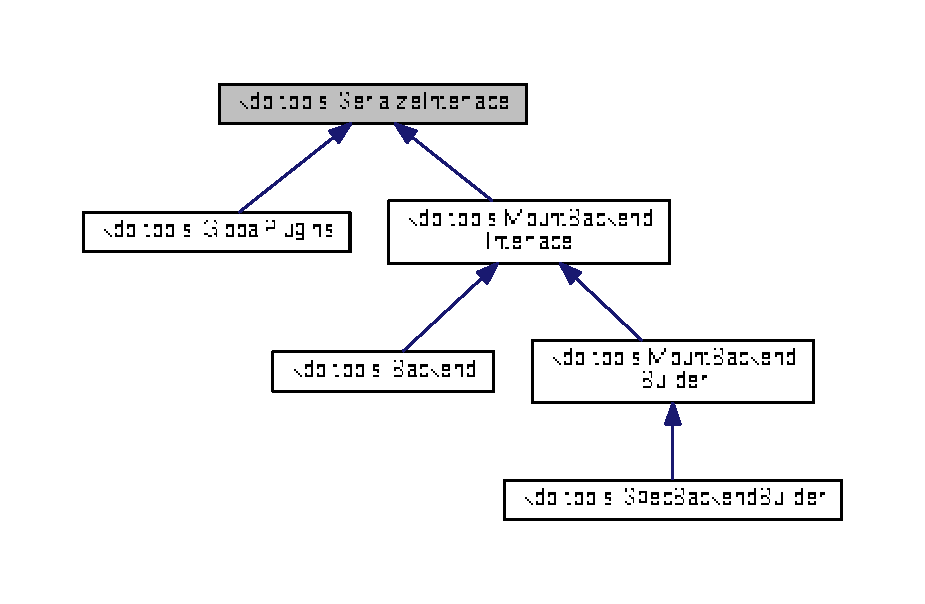
\includegraphics[width=350pt]{classkdb_1_1tools_1_1SerializeInterface__inherit__graph}
\end{center}
\end{figure}


\subsection{Detailed Description}
Interface to serialize a backend. 

The documentation for this class was generated from the following files\+:\begin{DoxyCompactItemize}
\item 
\mbox{\hyperlink{backend_8hpp}{backend.\+hpp}}\item 
\mbox{\hyperlink{src_2backend_8cpp}{src/backend.\+cpp}}\end{DoxyCompactItemize}

\hypertarget{classkdb_1_1tools_1_1SetPlugins}{}\section{kdb\+:\+:tools\+:\+:Set\+Plugins Class Reference}
\label{classkdb_1_1tools_1_1SetPlugins}\index{kdb\+::tools\+::\+Set\+Plugins@{kdb\+::tools\+::\+Set\+Plugins}}


\hyperlink{classkdb_1_1tools_1_1Plugins}{Plugins} to set configuration.  




{\ttfamily \#include $<$plugins.\+hpp$>$}



Inheritance diagram for kdb\+:\+:tools\+:\+:Set\+Plugins\+:
\nopagebreak
\begin{figure}[H]
\begin{center}
\leavevmode
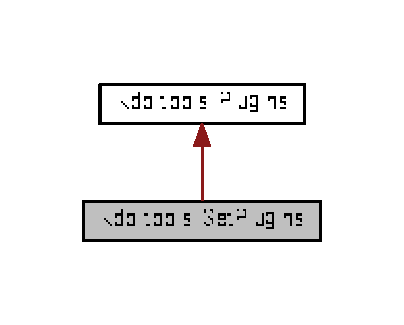
\includegraphics[width=194pt]{classkdb_1_1tools_1_1SetPlugins__inherit__graph}
\end{center}
\end{figure}


Collaboration diagram for kdb\+:\+:tools\+:\+:Set\+Plugins\+:
\nopagebreak
\begin{figure}[H]
\begin{center}
\leavevmode
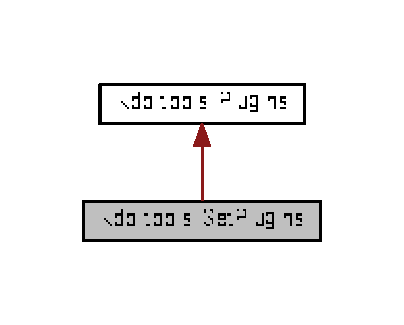
\includegraphics[width=194pt]{classkdb_1_1tools_1_1SetPlugins__coll__graph}
\end{center}
\end{figure}


\subsection{Detailed Description}
\hyperlink{classkdb_1_1tools_1_1Plugins}{Plugins} to set configuration. 

The documentation for this class was generated from the following files\+:\begin{DoxyCompactItemize}
\item 
\hyperlink{plugins_8hpp}{plugins.\+hpp}\item 
\hyperlink{plugins_8cpp}{plugins.\+cpp}\end{DoxyCompactItemize}

\hypertarget{classkdb_1_1SetPolicyIs}{\section{kdb\+:\+:Set\+Policy\+Is$<$ Policy $>$ Class Template Reference}
\label{classkdb_1_1SetPolicyIs}\index{kdb\+::\+Set\+Policy\+Is$<$ Policy $>$@{kdb\+::\+Set\+Policy\+Is$<$ Policy $>$}}
}


Needed by the user to set one of the policies.  




{\ttfamily \#include $<$kdbvalue.\+hpp$>$}



Inherits kdb\+::\+Default\+Policies.



\subsection{Detailed Description}
\subsubsection*{template$<$typename Policy$>$class kdb\+::\+Set\+Policy\+Is$<$ Policy $>$}

Needed by the user to set one of the policies. 


\begin{DoxyTemplParams}{Template Parameters}
{\em Policy} & \\
\hline
\end{DoxyTemplParams}


The documentation for this class was generated from the following file\+:\begin{DoxyCompactItemize}
\item 
kdbvalue.\+hpp\end{DoxyCompactItemize}

\hypertarget{classkdb_1_1tools_1_1SpecBackendBuilder}{}\doxysection{kdb\+::tools\+::Spec\+Backend\+Builder Class Reference}
\label{classkdb_1_1tools_1_1SpecBackendBuilder}\index{kdb::tools::SpecBackendBuilder@{kdb::tools::SpecBackendBuilder}}


Build individual backend while reading specification.  




{\ttfamily \#include $<$specreader.\+hpp$>$}



Inheritance diagram for kdb\+::tools\+::Spec\+Backend\+Builder\+:
\nopagebreak
\begin{figure}[H]
\begin{center}
\leavevmode
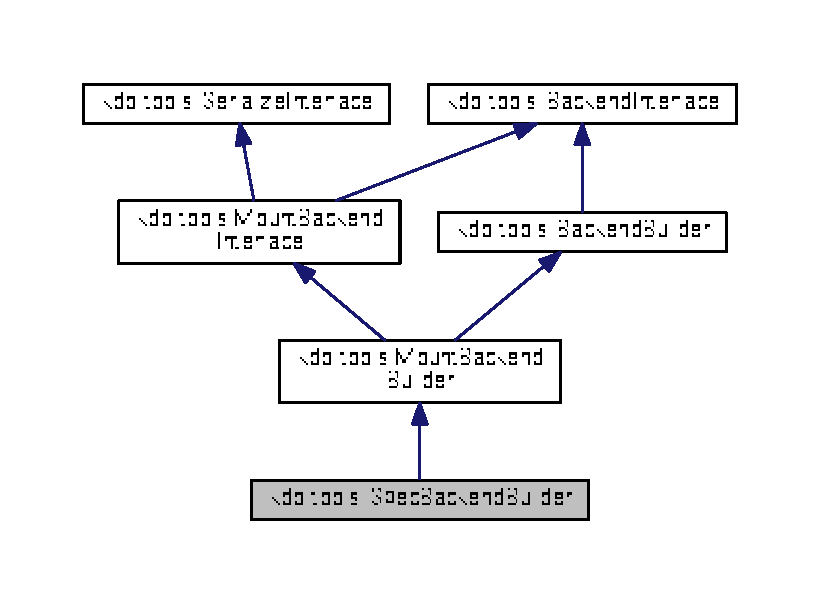
\includegraphics[width=350pt]{classkdb_1_1tools_1_1SpecBackendBuilder__inherit__graph}
\end{center}
\end{figure}


Collaboration diagram for kdb\+::tools\+::Spec\+Backend\+Builder\+:
\nopagebreak
\begin{figure}[H]
\begin{center}
\leavevmode
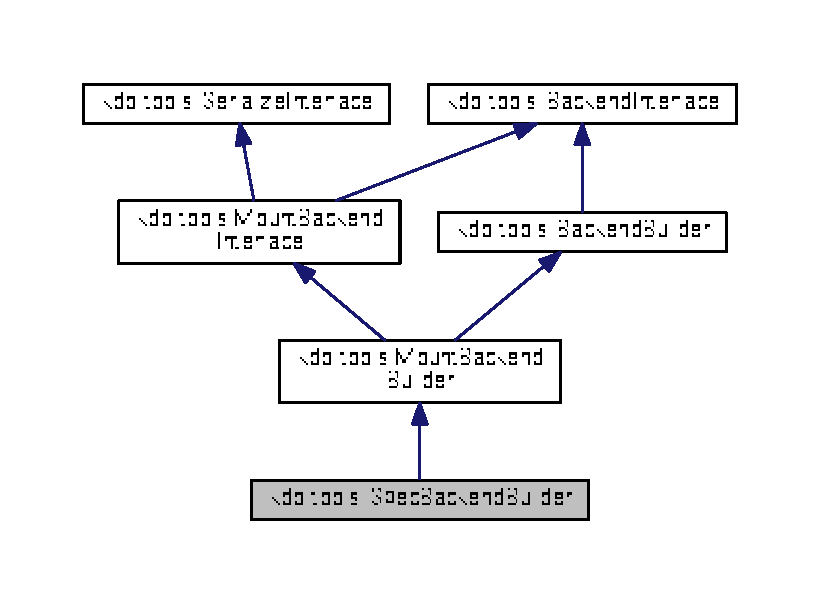
\includegraphics[width=350pt]{classkdb_1_1tools_1_1SpecBackendBuilder__coll__graph}
\end{center}
\end{figure}
\doxysubsection*{Additional Inherited Members}


\doxysubsection{Detailed Description}
Build individual backend while reading specification. 

The documentation for this class was generated from the following files\+:\begin{DoxyCompactItemize}
\item 
\mbox{\hyperlink{specreader_8hpp}{specreader.\+hpp}}\item 
specreader.\+cpp\end{DoxyCompactItemize}

\hypertarget{classkdb_1_1tools_1_1SpecReader}{}\section{kdb\+:\+:tools\+:\+:Spec\+Reader Class Reference}
\label{classkdb_1_1tools_1_1SpecReader}\index{kdb\+::tools\+::\+Spec\+Reader@{kdb\+::tools\+::\+Spec\+Reader}}


Highlevel interface to build a backend from specification.  




{\ttfamily \#include $<$specreader.\+hpp$>$}

\subsection*{Public Member Functions}
\begin{DoxyCompactItemize}
\item 
Backends \hyperlink{classkdb_1_1tools_1_1SpecReader_a0a1b4d2b7267d1dd4452f08fd898f0fd}{get\+Backends} ()
\item 
void \hyperlink{classkdb_1_1tools_1_1SpecReader_af0c638ed8094ebf3a5b4e028bbe2c38b}{read\+Specification} (\hyperlink{classkdb_1_1KeySet}{Key\+Set} const \&ks)
\begin{DoxyCompactList}\small\item\em Reads in a specification. \end{DoxyCompactList}\end{DoxyCompactItemize}


\subsection{Detailed Description}
Highlevel interface to build a backend from specification. 

\subsection{Member Function Documentation}
\mbox{\Hypertarget{classkdb_1_1tools_1_1SpecReader_a0a1b4d2b7267d1dd4452f08fd898f0fd}\label{classkdb_1_1tools_1_1SpecReader_a0a1b4d2b7267d1dd4452f08fd898f0fd}} 
\index{kdb\+::tools\+::\+Spec\+Reader@{kdb\+::tools\+::\+Spec\+Reader}!get\+Backends@{get\+Backends}}
\index{get\+Backends@{get\+Backends}!kdb\+::tools\+::\+Spec\+Reader@{kdb\+::tools\+::\+Spec\+Reader}}
\subsubsection{\texorpdfstring{get\+Backends()}{getBackends()}}
{\footnotesize\ttfamily Backends kdb\+::tools\+::\+Spec\+Reader\+::get\+Backends (\begin{DoxyParamCaption}{ }\end{DoxyParamCaption})\hspace{0.3cm}{\ttfamily [inline]}}

\begin{DoxyReturn}{Returns}
backends without resolved needs
\end{DoxyReturn}
\begin{DoxySeeAlso}{See also}
resolve\+Needs() 
\end{DoxySeeAlso}
\mbox{\Hypertarget{classkdb_1_1tools_1_1SpecReader_af0c638ed8094ebf3a5b4e028bbe2c38b}\label{classkdb_1_1tools_1_1SpecReader_af0c638ed8094ebf3a5b4e028bbe2c38b}} 
\index{kdb\+::tools\+::\+Spec\+Reader@{kdb\+::tools\+::\+Spec\+Reader}!read\+Specification@{read\+Specification}}
\index{read\+Specification@{read\+Specification}!kdb\+::tools\+::\+Spec\+Reader@{kdb\+::tools\+::\+Spec\+Reader}}
\subsubsection{\texorpdfstring{read\+Specification()}{readSpecification()}}
{\footnotesize\ttfamily void kdb\+::tools\+::\+Spec\+Reader\+::read\+Specification (\begin{DoxyParamCaption}\item[{\hyperlink{classkdb_1_1KeySet}{Key\+Set} const \&}]{ks }\end{DoxyParamCaption})}



Reads in a specification. 

Adds plugins using \hyperlink{classkdb_1_1tools_1_1BackendBuilder}{Backend\+Builder} during that.


\begin{DoxyParams}{Parameters}
{\em ks} & \\
\hline
\end{DoxyParams}


The documentation for this class was generated from the following files\+:\begin{DoxyCompactItemize}
\item 
\hyperlink{specreader_8hpp}{specreader.\+hpp}\item 
specreader.\+cpp\end{DoxyCompactItemize}

\hypertarget{classkdb_1_1ThreadSubject}{\section{kdb\-:\-:Thread\-Subject Class Reference}
\label{classkdb_1_1ThreadSubject}\index{kdb\-::\-Thread\-Subject@{kdb\-::\-Thread\-Subject}}
}


Subject from Observer pattern for Thread\-Context.  




{\ttfamily \#include $<$kdbthread.\-hpp$>$}



Inherited by kdb\-::\-Thread\-Context.



\subsection{Detailed Description}
Subject from Observer pattern for Thread\-Context. 

The documentation for this class was generated from the following file\-:\begin{DoxyCompactItemize}
\item 
kdbthread.\-hpp\end{DoxyCompactItemize}

\hypertarget{structkdb_1_1tools_1_1ToolException}{}\doxysection{kdb\+::tools\+::Tool\+Exception Struct Reference}
\label{structkdb_1_1tools_1_1ToolException}\index{kdb::tools::ToolException@{kdb::tools::ToolException}}


All exceptions from the elektratools library are derived from this exception.  




{\ttfamily \#include $<$toolexcept.\+hpp$>$}



Inherits std\+::runtime\+\_\+error.



Inherited by kdb\+::tools\+::\+Backend\+Check\+Exception, kdb\+::tools\+::\+Parse\+Exception, kdb\+::tools\+::\+Plugin\+Check\+Exception, kdb\+::tools\+::helper\+::\+Invalid\+Rebase\+Exception, and kdb\+::tools\+::merging\+::\+Invalid\+Conflict\+Operation.



\doxysubsection{Detailed Description}
All exceptions from the elektratools library are derived from this exception. 

The documentation for this struct was generated from the following file\+:\begin{DoxyCompactItemize}
\item 
\mbox{\hyperlink{toolexcept_8hpp}{toolexcept.\+hpp}}\end{DoxyCompactItemize}

\hypertarget{structkdb_1_1VaAlloc}{}\section{kdb\+:\+:Va\+Alloc Struct Reference}
\label{structkdb_1_1VaAlloc}\index{kdb\+::\+Va\+Alloc@{kdb\+::\+Va\+Alloc}}


Needed to avoid constructor ambiguity.  




{\ttfamily \#include $<$keyset.\+hpp$>$}



\subsection{Detailed Description}
Needed to avoid constructor ambiguity. 

when ... is same type as va\+\_\+list 

The documentation for this struct was generated from the following file\+:\begin{DoxyCompactItemize}
\item 
\hyperlink{keyset_8hpp}{keyset.\+hpp}\end{DoxyCompactItemize}

\hypertarget{classkdb_1_1ValueObserver}{}\doxysection{kdb\+::Value\+Observer Class Reference}
\label{classkdb_1_1ValueObserver}\index{kdb::ValueObserver@{kdb::ValueObserver}}


Base class for values to be observed.  




{\ttfamily \#include $<$kdbvalue.\+hpp$>$}



Inherited by kdb\+::\+Value$<$ T, Policy\+Setter1, Policy\+Setter2, Policy\+Setter3, Policy\+Setter4, Policy\+Setter5, Policy\+Setter6 $>$.



\doxysubsection{Detailed Description}
Base class for values to be observed. 

update\+Context() is called whenever a context tells a value that it should reevaluate its name and update its cache. 

The documentation for this class was generated from the following file\+:\begin{DoxyCompactItemize}
\item 
\mbox{\hyperlink{kdbvalue_8hpp}{kdbvalue.\+hpp}}\end{DoxyCompactItemize}

\hypertarget{classkdb_1_1Wrapped}{}\section{kdb\+::Wrapped Class Reference}
\label{classkdb_1_1Wrapped}\index{kdb::Wrapped@{kdb::Wrapped}}


Everything implementing this interface can be used as layer.  




{\ttfamily \#include $<$kdbvalue.\+hpp$>$}



Inherited by kdb\+::\+Value$<$ T, Policy\+Setter1, Policy\+Setter2, Policy\+Setter3, Policy\+Setter4, Policy\+Setter5, Policy\+Setter6 $>$.



\subsection{Detailed Description}
Everything implementing this interface can be used as layer. 

Different from \char`\"{}\+Layer\char`\"{} objects they will not be constructed on activation but instead only the Wrap\+Layer will be constructed and the wrapped object will be passed along by reference.

\begin{DoxyNote}{Note}
the lifetime must be beyond layer deactivation! 
\end{DoxyNote}


The documentation for this class was generated from the following file\+:\begin{DoxyCompactItemize}
\item 
\mbox{\hyperlink{kdbvalue_8hpp}{kdbvalue.\+hpp}}\end{DoxyCompactItemize}

\hypertarget{classkdb_1_1WritePolicyIs}{\section{kdb\+:\+:Write\+Policy\+Is$<$ Policy $>$ Class Template Reference}
\label{classkdb_1_1WritePolicyIs}\index{kdb\+::\+Write\+Policy\+Is$<$ Policy $>$@{kdb\+::\+Write\+Policy\+Is$<$ Policy $>$}}
}


Needed by the user to set one of the policies.  




{\ttfamily \#include $<$kdbvalue.\+hpp$>$}



Inherits kdb\+::\+Default\+Policies.



\subsection{Detailed Description}
\subsubsection*{template$<$typename Policy$>$class kdb\+::\+Write\+Policy\+Is$<$ Policy $>$}

Needed by the user to set one of the policies. 


\begin{DoxyTemplParams}{Template Parameters}
{\em Policy} & \\
\hline
\end{DoxyTemplParams}


The documentation for this class was generated from the following file\+:\begin{DoxyCompactItemize}
\item 
kdbvalue.\+hpp\end{DoxyCompactItemize}

\chapter{File Documentation}
\hypertarget{array_8c}{}\section{array.\+c File Reference}
\label{array_8c}\index{array.\+c@{array.\+c}}


Array methods.  


{\ttfamily \#include $<$kdb.\+h$>$}\newline
{\ttfamily \#include $<$kdbease.\+h$>$}\newline
{\ttfamily \#include $<$kdbhelper.\+h$>$}\newline
{\ttfamily \#include $<$kdbtypes.\+h$>$}\newline
{\ttfamily \#include $<$ctype.\+h$>$}\newline
{\ttfamily \#include $<$errno.\+h$>$}\newline
{\ttfamily \#include $<$limits.\+h$>$}\newline
{\ttfamily \#include $<$stdio.\+h$>$}\newline
{\ttfamily \#include $<$stdlib.\+h$>$}\newline
{\ttfamily \#include $<$string.\+h$>$}\newline
Include dependency graph for array.\+c\+:
\nopagebreak
\begin{figure}[H]
\begin{center}
\leavevmode
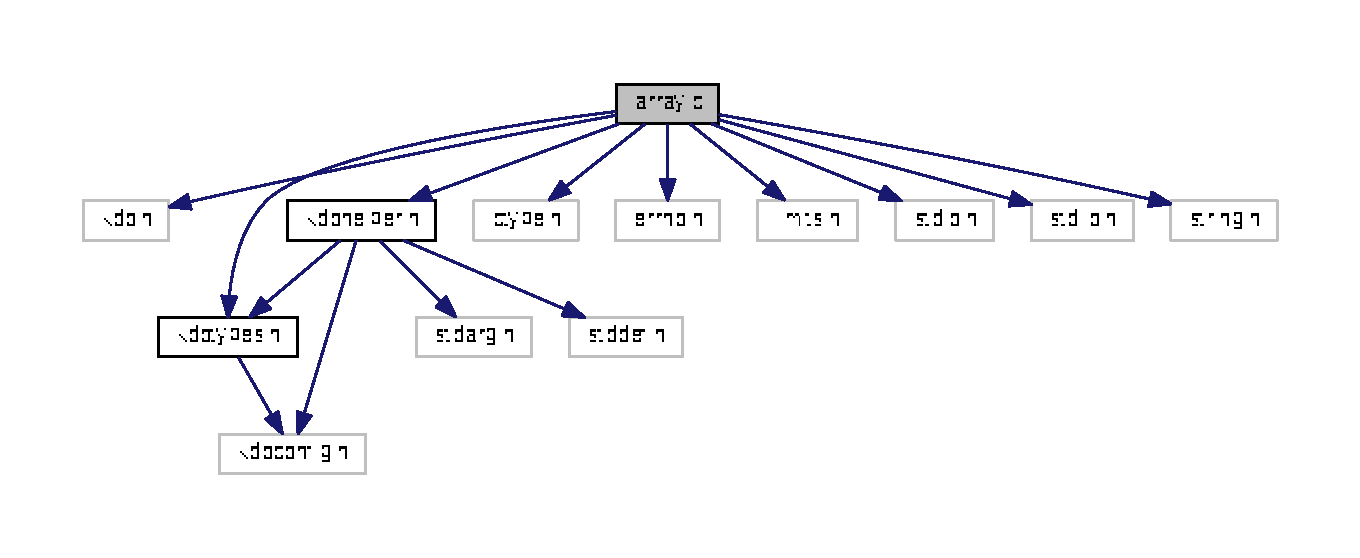
\includegraphics[width=350pt]{array_8c__incl}
\end{center}
\end{figure}
\subsection*{Functions}
\begin{DoxyCompactItemize}
\item 
int \hyperlink{array_8c_afc46476b8d722d89e07a966e023df317}{elektra\+Array\+Inc\+Name} (Key $\ast$key)
\begin{DoxyCompactList}\small\item\em Increment the name of the key by one. \end{DoxyCompactList}\item 
Key\+Set $\ast$ \hyperlink{array_8c_aee59442d3b1dea04454c7b93cd00c7ad}{elektra\+Array\+Get} (const Key $\ast$array\+Parent, Key\+Set $\ast$keys)
\begin{DoxyCompactList}\small\item\em Return all the array keys below the given array parent. \end{DoxyCompactList}\item 
Key $\ast$ \hyperlink{array_8c_aff4f7cbfc779e917ee41284d834231c6}{elektra\+Array\+Get\+Next\+Key} (Key\+Set $\ast$array\+Keys)
\begin{DoxyCompactList}\small\item\em Return the next key in the given array. \end{DoxyCompactList}\end{DoxyCompactItemize}


\subsection{Detailed Description}
Array methods. 

\begin{DoxyCopyright}{Copyright}
B\+SD License (see L\+I\+C\+E\+N\+S\+E.\+md or \href{https://www.libelektra.org}{\tt https\+://www.\+libelektra.\+org}) 
\end{DoxyCopyright}


\subsection{Function Documentation}
\mbox{\Hypertarget{array_8c_aee59442d3b1dea04454c7b93cd00c7ad}\label{array_8c_aee59442d3b1dea04454c7b93cd00c7ad}} 
\index{array.\+c@{array.\+c}!elektra\+Array\+Get@{elektra\+Array\+Get}}
\index{elektra\+Array\+Get@{elektra\+Array\+Get}!array.\+c@{array.\+c}}
\subsubsection{\texorpdfstring{elektra\+Array\+Get()}{elektraArrayGet()}}
{\footnotesize\ttfamily Key\+Set$\ast$ elektra\+Array\+Get (\begin{DoxyParamCaption}\item[{const Key $\ast$}]{array\+Parent,  }\item[{Key\+Set $\ast$}]{keys }\end{DoxyParamCaption})}



Return all the array keys below the given array parent. 

The array parent itself is not returned. For example, if {\ttfamily user/config/\#} is an array, {\ttfamily user/config} is the array parent. Only the direct array keys will be returned. This means that for example {\ttfamily user/config/\#1/key} will not be included, but only {\ttfamily user/config/\#1}.

A new keyset will be allocated for the resulting keys. This means that the caller must {\ttfamily ks\+Del} the resulting keyset.


\begin{DoxyParams}{Parameters}
{\em array\+Parent} & the parent of the array to be returned \\
\hline
{\em keys} & the keyset containing the array keys\\
\hline
\end{DoxyParams}
\begin{DoxyReturn}{Returns}
a keyset containing the array keys (if any) 
\end{DoxyReturn}

\begin{DoxyRetVals}{Return values}
{\em N\+U\+LL} & on {\ttfamily N\+U\+LL} pointers \\
\hline
\end{DoxyRetVals}
\mbox{\Hypertarget{array_8c_aff4f7cbfc779e917ee41284d834231c6}\label{array_8c_aff4f7cbfc779e917ee41284d834231c6}} 
\index{array.\+c@{array.\+c}!elektra\+Array\+Get\+Next\+Key@{elektra\+Array\+Get\+Next\+Key}}
\index{elektra\+Array\+Get\+Next\+Key@{elektra\+Array\+Get\+Next\+Key}!array.\+c@{array.\+c}}
\subsubsection{\texorpdfstring{elektra\+Array\+Get\+Next\+Key()}{elektraArrayGetNextKey()}}
{\footnotesize\ttfamily Key$\ast$ elektra\+Array\+Get\+Next\+Key (\begin{DoxyParamCaption}\item[{Key\+Set $\ast$}]{array\+Keys }\end{DoxyParamCaption})}



Return the next key in the given array. 

The function will automatically allocate memory for a new key and name it accordingly.

\begin{DoxyPrecond}{Precondition}
The supplied keyset must contain only valid array keys.
\end{DoxyPrecond}
The caller has to key\+Del the resulting key.


\begin{DoxyParams}{Parameters}
{\em array\+Keys} & the array where the new key will belong to\\
\hline
\end{DoxyParams}
\begin{DoxyReturn}{Returns}
the new array key on success 
\end{DoxyReturn}

\begin{DoxyRetVals}{Return values}
{\em N\+U\+LL} & if the passed array is empty \\
\hline
{\em N\+U\+LL} & on N\+U\+LL pointers or if an error occurs \\
\hline
\end{DoxyRetVals}
\mbox{\Hypertarget{array_8c_afc46476b8d722d89e07a966e023df317}\label{array_8c_afc46476b8d722d89e07a966e023df317}} 
\index{array.\+c@{array.\+c}!elektra\+Array\+Inc\+Name@{elektra\+Array\+Inc\+Name}}
\index{elektra\+Array\+Inc\+Name@{elektra\+Array\+Inc\+Name}!array.\+c@{array.\+c}}
\subsubsection{\texorpdfstring{elektra\+Array\+Inc\+Name()}{elektraArrayIncName()}}
{\footnotesize\ttfamily int elektra\+Array\+Inc\+Name (\begin{DoxyParamCaption}\item[{Key $\ast$}]{key }\end{DoxyParamCaption})}



Increment the name of the key by one. 

Alphabetical order will remain

e.\+g. user/abc/\#9 will be changed to user/abc/\#\+\_\+10

For the start\+: user/abc/\# will be changed to user/abc/\#0


\begin{DoxyParams}{Parameters}
{\em key} & which base name will be incremented\\
\hline
\end{DoxyParams}

\begin{DoxyRetVals}{Return values}
{\em -\/1} & on error (e.\+g. array too large, non-\/valid array) \\
\hline
{\em 0} & on success \\
\hline
\end{DoxyRetVals}

\hypertarget{automergeconfiguration_8cpp}{\section{automergeconfiguration.\+cpp File Reference}
\label{automergeconfiguration_8cpp}\index{automergeconfiguration.\+cpp@{automergeconfiguration.\+cpp}}
}
{\ttfamily \#include $<$merging/automergeconfiguration.\+hpp$>$}\\*
{\ttfamily \#include $<$merging/automergestrategy.\+hpp$>$}\\*
{\ttfamily \#include $<$merging/metamergestrategy.\+hpp$>$}\\*
Include dependency graph for automergeconfiguration.\+cpp\+:
\nopagebreak
\begin{figure}[H]
\begin{center}
\leavevmode
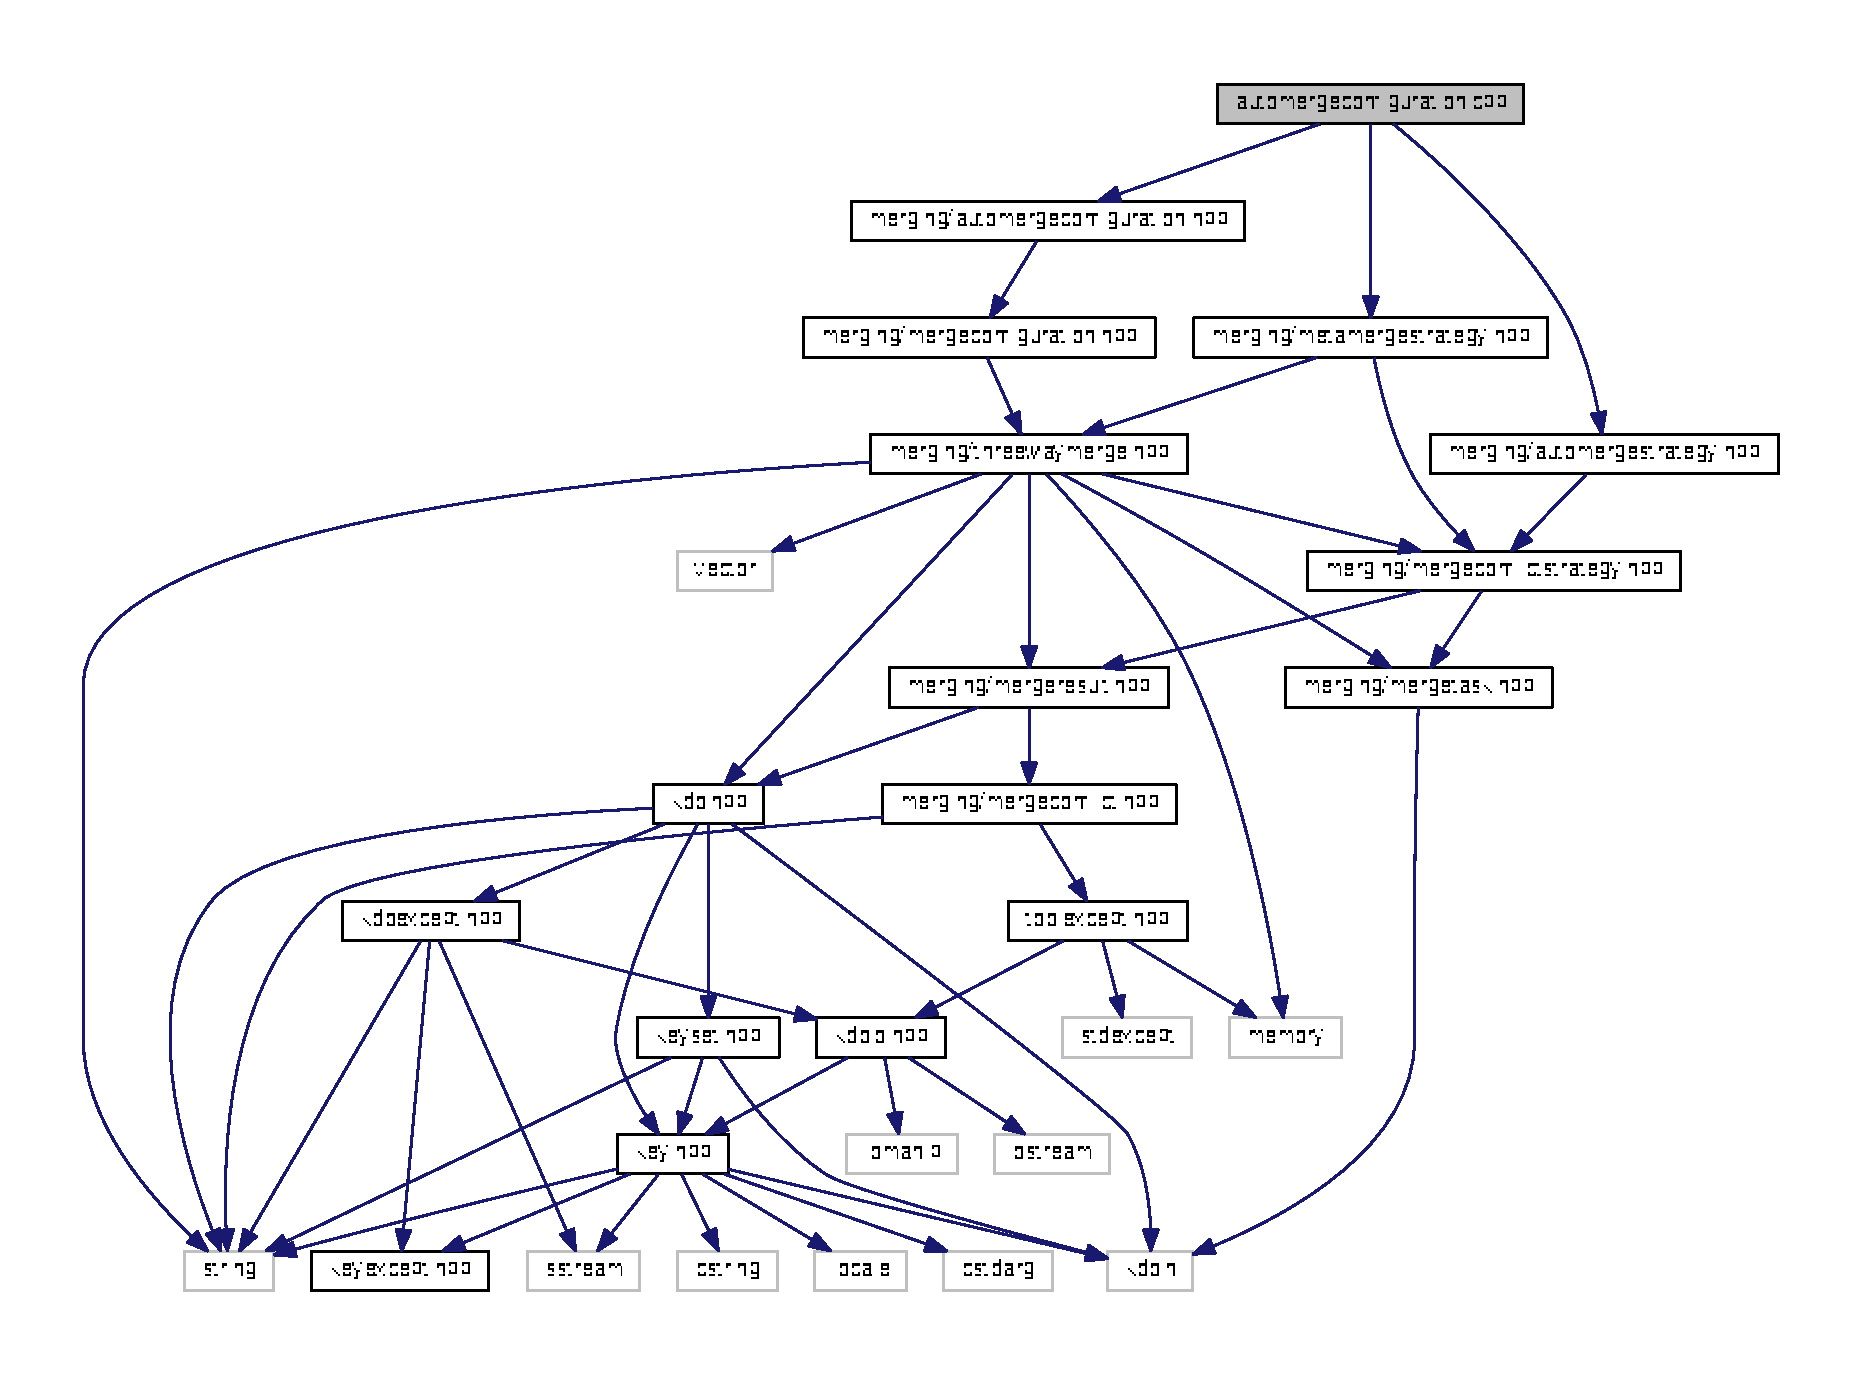
\includegraphics[width=350pt]{automergeconfiguration_8cpp__incl}
\end{center}
\end{figure}
\subsection*{Namespaces}
\begin{DoxyCompactItemize}
\item 
 \hyperlink{namespacekdb}{kdb}
\begin{DoxyCompactList}\small\item\em This is the main namespace for the C++ binding and libraries. \end{DoxyCompactList}\item 
 \hyperlink{namespacekdb_1_1tools}{kdb\+::tools}
\begin{DoxyCompactList}\small\item\em This namespace is for the libtool library. \end{DoxyCompactList}\end{DoxyCompactItemize}


\subsection{Detailed Description}
\begin{DoxyCopyright}{Copyright}
B\+S\+D License (see doc/\+C\+O\+P\+Y\+I\+N\+G or \href{http://www.libelektra.org}{\tt http\+://www.\+libelektra.\+org}) 
\end{DoxyCopyright}

\hypertarget{automergeconfiguration_8hpp}{\section{automergeconfiguration.\+hpp File Reference}
\label{automergeconfiguration_8hpp}\index{automergeconfiguration.\+hpp@{automergeconfiguration.\+hpp}}
}


A configuration for a simple automerge.  


{\ttfamily \#include $<$merging/mergeconfiguration.\+hpp$>$}\\*
Include dependency graph for automergeconfiguration.\+hpp\+:
\nopagebreak
\begin{figure}[H]
\begin{center}
\leavevmode
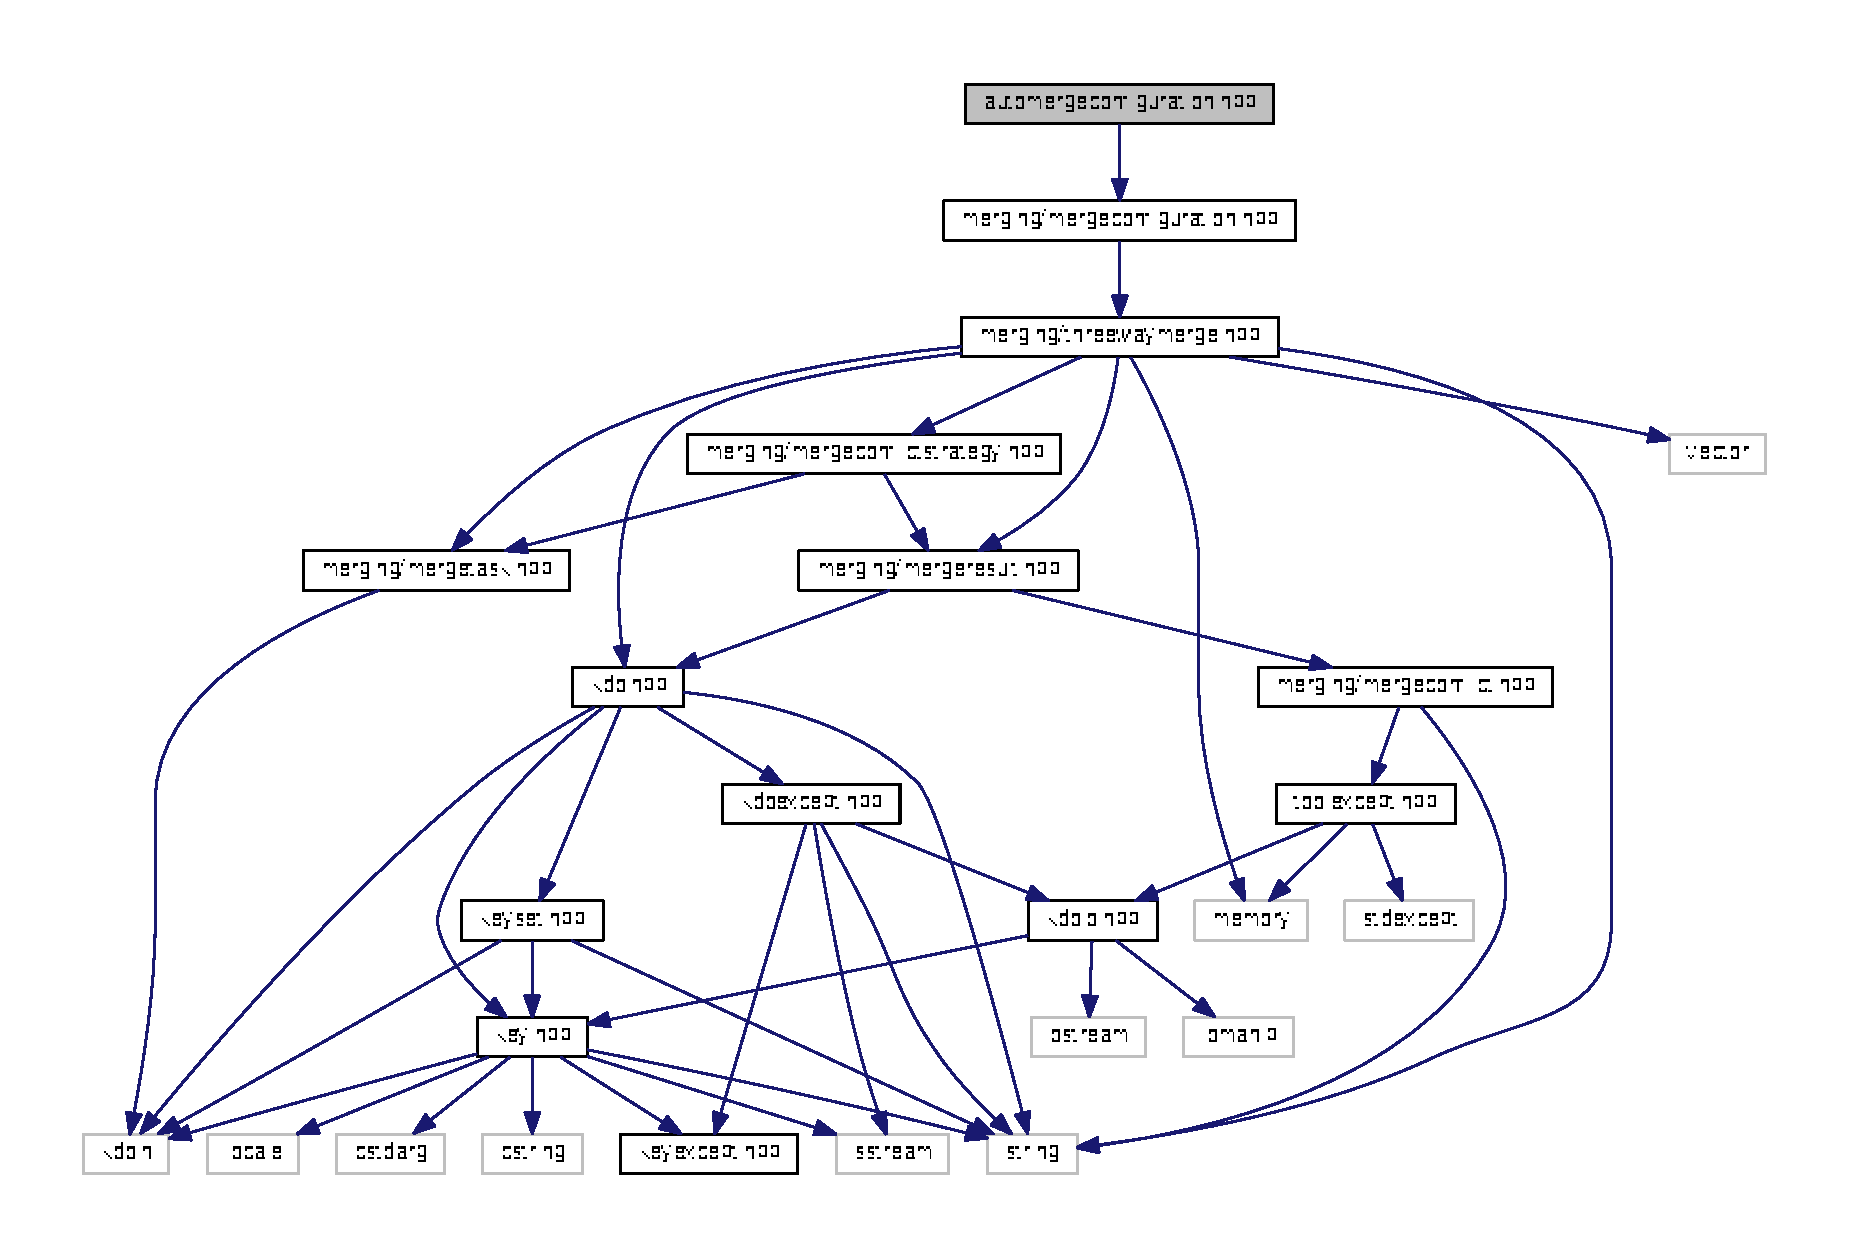
\includegraphics[width=350pt]{automergeconfiguration_8hpp__incl}
\end{center}
\end{figure}
This graph shows which files directly or indirectly include this file\+:
\nopagebreak
\begin{figure}[H]
\begin{center}
\leavevmode
\includegraphics[width=350pt]{automergeconfiguration_8hpp__dep__incl}
\end{center}
\end{figure}
\subsection*{Namespaces}
\begin{DoxyCompactItemize}
\item 
 \hyperlink{namespacekdb}{kdb}
\begin{DoxyCompactList}\small\item\em This is the main namespace for the C++ binding and libraries. \end{DoxyCompactList}\item 
 \hyperlink{namespacekdb_1_1tools}{kdb\+::tools}
\begin{DoxyCompactList}\small\item\em This namespace is for the libtool library. \end{DoxyCompactList}\end{DoxyCompactItemize}


\subsection{Detailed Description}
A configuration for a simple automerge. 

\begin{DoxyCopyright}{Copyright}
B\+S\+D License (see doc/\+C\+O\+P\+Y\+I\+N\+G or \href{http://www.libelektra.org}{\tt http\+://www.\+libelektra.\+org}) 
\end{DoxyCopyright}

\hypertarget{automergestrategy_8cpp}{}\doxysection{automergestrategy.\+cpp File Reference}
\label{automergestrategy_8cpp}\index{automergestrategy.cpp@{automergestrategy.cpp}}


Implementation of Auto\+Merge\+Strategy.  


{\ttfamily \#include $<$helper/keyhelper.\+hpp$>$}\newline
{\ttfamily \#include $<$merging/automergestrategy.\+hpp$>$}\newline
{\ttfamily \#include $<$string$>$}\newline
Include dependency graph for automergestrategy.\+cpp\+:
\nopagebreak
\begin{figure}[H]
\begin{center}
\leavevmode
\includegraphics[width=350pt]{automergestrategy_8cpp__incl}
\end{center}
\end{figure}
\doxysubsection*{Namespaces}
\begin{DoxyCompactItemize}
\item 
 \mbox{\hyperlink{namespacekdb}{kdb}}
\begin{DoxyCompactList}\small\item\em This is the main namespace for the C++ binding and libraries. \end{DoxyCompactList}\item 
 \mbox{\hyperlink{namespacekdb_1_1tools}{kdb\+::tools}}
\begin{DoxyCompactList}\small\item\em This namespace is for the libtool library. \end{DoxyCompactList}\end{DoxyCompactItemize}


\doxysubsection{Detailed Description}
Implementation of Auto\+Merge\+Strategy. 

\begin{DoxyCopyright}{Copyright}
B\+SD License (see L\+I\+C\+E\+N\+S\+E.\+md or \href{https://www.libelektra.org}{\texttt{ https\+://www.\+libelektra.\+org}}) 
\end{DoxyCopyright}

\hypertarget{automergestrategy_8hpp}{\section{automergestrategy.\+hpp File Reference}
\label{automergestrategy_8hpp}\index{automergestrategy.\+hpp@{automergestrategy.\+hpp}}
}


A strategy for taking the value of.  


{\ttfamily \#include $<$merging/mergeconflictstrategy.\+hpp$>$}\\*
Include dependency graph for automergestrategy.\+hpp\+:
\nopagebreak
\begin{figure}[H]
\begin{center}
\leavevmode
\includegraphics[width=350pt]{automergestrategy_8hpp__incl}
\end{center}
\end{figure}
This graph shows which files directly or indirectly include this file\+:
\nopagebreak
\begin{figure}[H]
\begin{center}
\leavevmode
\includegraphics[width=350pt]{automergestrategy_8hpp__dep__incl}
\end{center}
\end{figure}
\subsection*{Namespaces}
\begin{DoxyCompactItemize}
\item 
 \hyperlink{namespacekdb}{kdb}
\begin{DoxyCompactList}\small\item\em This is the main namespace for the C++ binding and libraries. \end{DoxyCompactList}\item 
 \hyperlink{namespacekdb_1_1tools}{kdb\+::tools}
\begin{DoxyCompactList}\small\item\em This namespace is for the libtool library. \end{DoxyCompactList}\end{DoxyCompactItemize}


\subsection{Detailed Description}
A strategy for taking the value of. 

\begin{DoxyCopyright}{Copyright}
B\+S\+D License (see doc/\+L\+I\+C\+E\+N\+S\+E.\+md or \href{http://www.libelektra.org}{\tt http\+://www.\+libelektra.\+org}) 
\end{DoxyCopyright}

\hypertarget{backend_8c}{}\section{backend.\+c File Reference}
\label{backend_8c}\index{backend.\+c@{backend.\+c}}


Everything related to a backend.  


{\ttfamily \#include $<$kdbassert.\+h$>$}\newline
{\ttfamily \#include $<$kdbinternal.\+h$>$}\newline
Include dependency graph for backend.\+c\+:
\nopagebreak
\begin{figure}[H]
\begin{center}
\leavevmode
\includegraphics[width=350pt]{backend_8c__incl}
\end{center}
\end{figure}
\subsection*{Functions}
\begin{DoxyCompactItemize}
\item 
int \hyperlink{backend_8c_aa81c8c0b5a2d0c59ea501f15049699b6}{elektra\+Backend\+Set\+Mountpoint} (Backend $\ast$backend, Key\+Set $\ast$elektra\+Config, Key $\ast$error\+Key)
\begin{DoxyCompactList}\small\item\em sets mountpoint \end{DoxyCompactList}\item 
Backend $\ast$ \hyperlink{backend_8c_a18a6369d1c2af977107fe475925a3393}{backend\+Open} (Key\+Set $\ast$elektra\+Config, Key\+Set $\ast$modules, Key\+Set $\ast$global, Key $\ast$error\+Key)
\begin{DoxyCompactList}\small\item\em Builds a backend out of the configuration supplied from\+: \end{DoxyCompactList}\item 
Backend $\ast$ \hyperlink{backend_8c_a5227608d302910f25fc3a5c8968ab542}{backend\+Open\+Default} (Key\+Set $\ast$modules, Key\+Set $\ast$global, const char $\ast$file, Key $\ast$error\+Key)
\begin{DoxyCompactList}\small\item\em Opens a default backend using the plugin named K\+D\+B\+\_\+\+R\+E\+S\+O\+L\+V\+ER and K\+D\+B\+\_\+\+S\+T\+O\+R\+A\+GE. \end{DoxyCompactList}\item 
Backend $\ast$ \hyperlink{backend_8c_ae8fb4357da3f748492e9f5300a537369}{backend\+Open\+Modules} (Key\+Set $\ast$modules, Key\+Set $\ast$global, Key $\ast$error\+Key)
\item 
Backend $\ast$ \hyperlink{backend_8c_ad17f21b41a12609232573971823089e0}{backend\+Open\+Version} (Key\+Set $\ast$global, Key $\ast$error\+Key)
\begin{DoxyCompactList}\small\item\em Opens the internal version backend. \end{DoxyCompactList}\item 
int \hyperlink{backend_8c_a051ae3b70fe43b1632b975fb4c26535c}{backend\+Update\+Size} (Backend $\ast$backend, Key $\ast$parent, int size)
\begin{DoxyCompactList}\small\item\em Update internal size in backend. \end{DoxyCompactList}\end{DoxyCompactItemize}


\subsection{Detailed Description}
Everything related to a backend. 

\begin{DoxyCopyright}{Copyright}
B\+SD License (see L\+I\+C\+E\+N\+S\+E.\+md or \href{https://www.libelektra.org}{\tt https\+://www.\+libelektra.\+org}) 
\end{DoxyCopyright}


\subsection{Function Documentation}
\mbox{\Hypertarget{backend_8c_a18a6369d1c2af977107fe475925a3393}\label{backend_8c_a18a6369d1c2af977107fe475925a3393}} 
\index{backend.\+c@{backend.\+c}!backend\+Open@{backend\+Open}}
\index{backend\+Open@{backend\+Open}!backend.\+c@{backend.\+c}}
\subsubsection{\texorpdfstring{backend\+Open()}{backendOpen()}}
{\footnotesize\ttfamily Backend$\ast$ backend\+Open (\begin{DoxyParamCaption}\item[{Key\+Set $\ast$}]{elektra\+Config,  }\item[{Key\+Set $\ast$}]{modules,  }\item[{Key\+Set $\ast$}]{global,  }\item[{Key $\ast$}]{error\+Key }\end{DoxyParamCaption})}



Builds a backend out of the configuration supplied from\+: 

\begin{DoxyVerb}system/elektra/mountpoints/<name>
\end{DoxyVerb}


The root key must be like the above example. You do not need to rewind the keyset. But every key must be below the root key.

The internal consistency will be checked in this function. If necessary parts are missing, like no plugins, they cant be loaded or similar 0 will be returned.

\hyperlink{group__keyset_ga6b00cf82b59af4d883a9bad6cf4a4a4a}{ks\+Cut()} is perfectly suitable for cutting out the configuration like needed.

\begin{DoxyNote}{Note}
The given Key\+Set will be deleted within the function, don\textquotesingle{}t use it afterwards.
\end{DoxyNote}

\begin{DoxyParams}{Parameters}
{\em elektra\+Config} & the configuration to work with. It is used to build up this backend. \\
\hline
{\em modules} & used to load new modules or get references to existing one \\
\hline
{\em global} & the global keyset of the K\+DB instance \\
\hline
{\em error\+Key} & the key where an error and warnings are added\\
\hline
\end{DoxyParams}
\begin{DoxyReturn}{Returns}
a pointer to a freshly allocated backend this could be the requested backend or a so called \char`\"{}missing backend\char`\"{}. 
\end{DoxyReturn}

\begin{DoxyRetVals}{Return values}
{\em 0} & if out of memory \\
\hline
\end{DoxyRetVals}
\mbox{\Hypertarget{backend_8c_a5227608d302910f25fc3a5c8968ab542}\label{backend_8c_a5227608d302910f25fc3a5c8968ab542}} 
\index{backend.\+c@{backend.\+c}!backend\+Open\+Default@{backend\+Open\+Default}}
\index{backend\+Open\+Default@{backend\+Open\+Default}!backend.\+c@{backend.\+c}}
\subsubsection{\texorpdfstring{backend\+Open\+Default()}{backendOpenDefault()}}
{\footnotesize\ttfamily Backend$\ast$ backend\+Open\+Default (\begin{DoxyParamCaption}\item[{Key\+Set $\ast$}]{modules,  }\item[{Key\+Set $\ast$}]{global,  }\item[{const char $\ast$}]{file,  }\item[{Key $\ast$}]{error\+Key }\end{DoxyParamCaption})}



Opens a default backend using the plugin named K\+D\+B\+\_\+\+R\+E\+S\+O\+L\+V\+ER and K\+D\+B\+\_\+\+S\+T\+O\+R\+A\+GE. 


\begin{DoxyParams}{Parameters}
{\em modules} & the modules to work with \\
\hline
{\em global} & the global keyset of the K\+DB instance \\
\hline
{\em error\+Key} & the key to issue warnings and errors to \\
\hline
\end{DoxyParams}
\begin{DoxyReturn}{Returns}
the fresh allocated default backend or 0 if it failed 
\end{DoxyReturn}
\mbox{\Hypertarget{backend_8c_ae8fb4357da3f748492e9f5300a537369}\label{backend_8c_ae8fb4357da3f748492e9f5300a537369}} 
\index{backend.\+c@{backend.\+c}!backend\+Open\+Modules@{backend\+Open\+Modules}}
\index{backend\+Open\+Modules@{backend\+Open\+Modules}!backend.\+c@{backend.\+c}}
\subsubsection{\texorpdfstring{backend\+Open\+Modules()}{backendOpenModules()}}
{\footnotesize\ttfamily Backend$\ast$ backend\+Open\+Modules (\begin{DoxyParamCaption}\item[{Key\+Set $\ast$}]{modules,  }\item[{Key\+Set $\ast$}]{global,  }\item[{Key $\ast$}]{error\+Key }\end{DoxyParamCaption})}

\begin{DoxyReturn}{Returns}
a backend which gives plugin configuration of the module which is currently point to.
\end{DoxyReturn}

\begin{DoxyParams}{Parameters}
{\em modules} & the modules to work with \\
\hline
{\em global} & the global keyset of the K\+DB instance \\
\hline
{\em error\+Key} & the key to issue warnings and errors to \\
\hline
\end{DoxyParams}
\mbox{\Hypertarget{backend_8c_ad17f21b41a12609232573971823089e0}\label{backend_8c_ad17f21b41a12609232573971823089e0}} 
\index{backend.\+c@{backend.\+c}!backend\+Open\+Version@{backend\+Open\+Version}}
\index{backend\+Open\+Version@{backend\+Open\+Version}!backend.\+c@{backend.\+c}}
\subsubsection{\texorpdfstring{backend\+Open\+Version()}{backendOpenVersion()}}
{\footnotesize\ttfamily Backend$\ast$ backend\+Open\+Version (\begin{DoxyParamCaption}\item[{Key\+Set $\ast$}]{global,  }\item[{Key $\ast$}]{error\+Key }\end{DoxyParamCaption})}



Opens the internal version backend. 


\begin{DoxyParams}{Parameters}
{\em global} & the global keyset of the K\+DB instance \\
\hline
{\em error\+Key} & the key to issue warnings and errors to \\
\hline
\end{DoxyParams}
\begin{DoxyReturn}{Returns}
the fresh allocated default backend or 0 if it failed 
\end{DoxyReturn}
\mbox{\Hypertarget{backend_8c_a051ae3b70fe43b1632b975fb4c26535c}\label{backend_8c_a051ae3b70fe43b1632b975fb4c26535c}} 
\index{backend.\+c@{backend.\+c}!backend\+Update\+Size@{backend\+Update\+Size}}
\index{backend\+Update\+Size@{backend\+Update\+Size}!backend.\+c@{backend.\+c}}
\subsubsection{\texorpdfstring{backend\+Update\+Size()}{backendUpdateSize()}}
{\footnotesize\ttfamily int backend\+Update\+Size (\begin{DoxyParamCaption}\item[{Backend $\ast$}]{backend,  }\item[{Key $\ast$}]{parent,  }\item[{int}]{size }\end{DoxyParamCaption})}



Update internal size in backend. 


\begin{DoxyParams}{Parameters}
{\em backend} & the backend to update \\
\hline
{\em parent} & for parent \\
\hline
{\em size} & to update (-\/1 default, 0 empty, $>$0 otherwise)\\
\hline
\end{DoxyParams}
\begin{DoxyPrecond}{Precondition}
parent must be serializable namespace
\end{DoxyPrecond}

\begin{DoxyRetVals}{Return values}
{\em -\/1} & if invalid parent (assert) \\
\hline
{\em 0} & on success \\
\hline
\end{DoxyRetVals}
\mbox{\Hypertarget{backend_8c_aa81c8c0b5a2d0c59ea501f15049699b6}\label{backend_8c_aa81c8c0b5a2d0c59ea501f15049699b6}} 
\index{backend.\+c@{backend.\+c}!elektra\+Backend\+Set\+Mountpoint@{elektra\+Backend\+Set\+Mountpoint}}
\index{elektra\+Backend\+Set\+Mountpoint@{elektra\+Backend\+Set\+Mountpoint}!backend.\+c@{backend.\+c}}
\subsubsection{\texorpdfstring{elektra\+Backend\+Set\+Mountpoint()}{elektraBackendSetMountpoint()}}
{\footnotesize\ttfamily int elektra\+Backend\+Set\+Mountpoint (\begin{DoxyParamCaption}\item[{Backend $\ast$}]{backend,  }\item[{Key\+Set $\ast$}]{elektra\+Config,  }\item[{Key $\ast$}]{error\+Key }\end{DoxyParamCaption})}



sets mountpoint 


\begin{DoxyParams}[1]{Parameters}
 & {\em backend} & where the mountpoint should be set \\
\hline
 & {\em elektra\+Config} & the config where the mountpoint can be found \\
\hline
\mbox{\tt out}  & {\em error\+Key} & the name also has the mountpoint set\\
\hline
\end{DoxyParams}
\begin{DoxyPrecond}{Precondition}
\hyperlink{group__keyset_ga4287b9416912c5f2ab9c195cb74fb094}{ks\+Current()} is root key 
\end{DoxyPrecond}
\begin{DoxyPostcond}{Postcondition}
\hyperlink{group__keyset_ga4287b9416912c5f2ab9c195cb74fb094}{ks\+Current()} is root key
\end{DoxyPostcond}

\begin{DoxyRetVals}{Return values}
{\em -\/1} & if no mountpoint is found or memory allocation problem \\
\hline
{\em 0} & on success \\
\hline
\end{DoxyRetVals}

\hypertarget{examples_2backend_8cpp}{}\doxysection{backend.\+cpp File Reference}
\label{examples_2backend_8cpp}\index{backend.cpp@{backend.cpp}}
{\ttfamily \#include $<$backendbuilder.\+hpp$>$}\newline
{\ttfamily \#include $<$backends.\+hpp$>$}\newline
{\ttfamily \#include $<$iostream$>$}\newline
Include dependency graph for examples/backend.cpp\+:
\nopagebreak
\begin{figure}[H]
\begin{center}
\leavevmode
\includegraphics[width=350pt]{examples_2backend_8cpp__incl}
\end{center}
\end{figure}


\doxysubsection{Detailed Description}
\begin{DoxyCopyright}{Copyright}
B\+SD License (see L\+I\+C\+E\+N\+S\+E.\+md or \href{https://www.libelektra.org}{\texttt{ https\+://www.\+libelektra.\+org}}) 
\end{DoxyCopyright}

\hypertarget{src_2backend_8cpp}{\section{backend.\+cpp File Reference}
\label{src_2backend_8cpp}\index{backend.\+cpp@{backend.\+cpp}}
}


Implementation of backend.  


{\ttfamily \#include $<$backend.\+hpp$>$}\\*
{\ttfamily \#include $<$backends.\+hpp$>$}\\*
{\ttfamily \#include $<$kdbmodule.\+h$>$}\\*
{\ttfamily \#include $<$kdbplugin.\+h$>$}\\*
{\ttfamily \#include $<$kdbprivate.\+h$>$}\\*
{\ttfamily \#include $<$helper/keyhelper.\+hpp$>$}\\*
{\ttfamily \#include $<$kdbease.\+h$>$}\\*
{\ttfamily \#include $<$algorithm$>$}\\*
{\ttfamily \#include $<$kdb.\+hpp$>$}\\*
{\ttfamily \#include $<$cassert$>$}\\*
Include dependency graph for src/backend.cpp\+:
\nopagebreak
\begin{figure}[H]
\begin{center}
\leavevmode
\includegraphics[width=350pt]{src_2backend_8cpp__incl}
\end{center}
\end{figure}
\subsection*{Namespaces}
\begin{DoxyCompactItemize}
\item 
 \hyperlink{namespacekdb}{kdb}
\begin{DoxyCompactList}\small\item\em This is the main namespace for the C++ binding and libraries. \end{DoxyCompactList}\item 
 \hyperlink{namespacekdb_1_1tools}{kdb\+::tools}
\begin{DoxyCompactList}\small\item\em This namespace is for the libtool library. \end{DoxyCompactList}\end{DoxyCompactItemize}
\subsection*{Functions}
\begin{DoxyCompactItemize}
\item 
std\+::ostream \& \hyperlink{namespacekdb_1_1tools_a10b59213ee542e33c7ecc481d4476a79}{kdb\+::tools\+::operator$<$$<$} (std\+::ostream \&os, Backend const \&b)
\begin{DoxyCompactList}\small\item\em Prints the current status. \end{DoxyCompactList}\end{DoxyCompactItemize}


\subsection{Detailed Description}
Implementation of backend. 

\begin{DoxyCopyright}{Copyright}
B\+S\+D License (see doc/\+C\+O\+P\+Y\+I\+N\+G or \href{http://www.libelektra.org}{\tt http\+://www.\+libelektra.\+org}) 
\end{DoxyCopyright}

\hypertarget{backend_8hpp}{\section{backend.\+hpp File Reference}
\label{backend_8hpp}\index{backend.\+hpp@{backend.\+hpp}}
}


Implements a way to build and deal with a backend.  


{\ttfamily \#include $<$plugins.\+hpp$>$}\\*
{\ttfamily \#include $<$modules.\+hpp$>$}\\*
{\ttfamily \#include $<$toolexcept.\+hpp$>$}\\*
{\ttfamily \#include $<$ostream$>$}\\*
{\ttfamily \#include $<$string$>$}\\*
{\ttfamily \#include $<$kdb.\+hpp$>$}\\*
Include dependency graph for backend.\+hpp\+:
\nopagebreak
\begin{figure}[H]
\begin{center}
\leavevmode
\includegraphics[width=350pt]{backend_8hpp__incl}
\end{center}
\end{figure}
This graph shows which files directly or indirectly include this file\+:
\nopagebreak
\begin{figure}[H]
\begin{center}
\leavevmode
\includegraphics[width=350pt]{backend_8hpp__dep__incl}
\end{center}
\end{figure}
\subsection*{Data Structures}
\begin{DoxyCompactItemize}
\item 
class \hyperlink{classkdb_1_1tools_1_1Backend}{kdb\+::tools\+::\+Backend}
\begin{DoxyCompactList}\small\item\em A representation of the backend (= set of plugins) that can be mounted. \end{DoxyCompactList}\end{DoxyCompactItemize}
\subsection*{Namespaces}
\begin{DoxyCompactItemize}
\item 
 \hyperlink{namespacekdb}{kdb}
\begin{DoxyCompactList}\small\item\em This is the main namespace for the C++ binding and libraries. \end{DoxyCompactList}\item 
 \hyperlink{namespacekdb_1_1tools}{kdb\+::tools}
\begin{DoxyCompactList}\small\item\em This namespace is for the libtool library. \end{DoxyCompactList}\end{DoxyCompactItemize}
\subsection*{Functions}
\begin{DoxyCompactItemize}
\item 
std\+::ostream \& \hyperlink{namespacekdb_1_1tools_a10b59213ee542e33c7ecc481d4476a79}{kdb\+::tools\+::operator$<$$<$} (std\+::ostream \&os, Backend const \&b)
\begin{DoxyCompactList}\small\item\em Prints the current status. \end{DoxyCompactList}\end{DoxyCompactItemize}


\subsection{Detailed Description}
Implements a way to build and deal with a backend. 

\begin{DoxyCopyright}{Copyright}
B\+S\+D License (see doc/\+C\+O\+P\+Y\+I\+N\+G or \href{http://www.libelektra.org}{\tt http\+://www.\+libelektra.\+org}) 
\end{DoxyCopyright}

\hypertarget{backendbuilder_8cpp}{\section{backendbuilder.\+cpp File Reference}
\label{backendbuilder_8cpp}\index{backendbuilder.\+cpp@{backendbuilder.\+cpp}}
}


Implementation of backend builder.  


{\ttfamily \#include $<$backend.\+hpp$>$}\\*
{\ttfamily \#include $<$backends.\+hpp$>$}\\*
{\ttfamily \#include $<$pluginspec.\+hpp$>$}\\*
{\ttfamily \#include $<$backendparser.\+hpp$>$}\\*
{\ttfamily \#include $<$backendbuilder.\+hpp$>$}\\*
{\ttfamily \#include $<$plugindatabase.\+hpp$>$}\\*
{\ttfamily \#include $<$kdbmodule.\+h$>$}\\*
{\ttfamily \#include $<$kdbplugin.\+h$>$}\\*
{\ttfamily \#include $<$kdbprivate.\+h$>$}\\*
{\ttfamily \#include $<$helper/keyhelper.\+hpp$>$}\\*
{\ttfamily \#include $<$set$>$}\\*
{\ttfamily \#include $<$algorithm$>$}\\*
{\ttfamily \#include $<$functional$>$}\\*
{\ttfamily \#include $<$kdb.\+hpp$>$}\\*
{\ttfamily \#include $<$cassert$>$}\\*
Include dependency graph for backendbuilder.\+cpp\+:
\nopagebreak
\begin{figure}[H]
\begin{center}
\leavevmode
\includegraphics[width=350pt]{backendbuilder_8cpp__incl}
\end{center}
\end{figure}
\subsection*{Namespaces}
\begin{DoxyCompactItemize}
\item 
 \hyperlink{namespacekdb}{kdb}
\begin{DoxyCompactList}\small\item\em This is the main namespace for the C++ binding and libraries. \end{DoxyCompactList}\item 
 \hyperlink{namespacekdb_1_1tools}{kdb\+::tools}
\begin{DoxyCompactList}\small\item\em This namespace is for the libtool library. \end{DoxyCompactList}\end{DoxyCompactItemize}


\subsection{Detailed Description}
Implementation of backend builder. 

\begin{DoxyCopyright}{Copyright}
B\+S\+D License (see doc/\+C\+O\+P\+Y\+I\+N\+G or \href{http://www.libelektra.org}{\tt http\+://www.\+libelektra.\+org}) 
\end{DoxyCopyright}

\hypertarget{backendbuilder_8hpp}{}\section{backendbuilder.\+hpp File Reference}
\label{backendbuilder_8hpp}\index{backendbuilder.hpp@{backendbuilder.hpp}}


Implements a way to build backends.  


{\ttfamily \#include $<$memory$>$}\newline
{\ttfamily \#include $<$set$>$}\newline
{\ttfamily \#include $<$vector$>$}\newline
{\ttfamily \#include $<$kdb.\+hpp$>$}\newline
{\ttfamily \#include $<$backend.\+hpp$>$}\newline
{\ttfamily \#include $<$plugin.\+hpp$>$}\newline
{\ttfamily \#include $<$plugindatabase.\+hpp$>$}\newline
{\ttfamily \#include $<$pluginspec.\+hpp$>$}\newline
Include dependency graph for backendbuilder.\+hpp\+:
\nopagebreak
\begin{figure}[H]
\begin{center}
\leavevmode
\includegraphics[width=350pt]{backendbuilder_8hpp__incl}
\end{center}
\end{figure}
This graph shows which files directly or indirectly include this file\+:
\nopagebreak
\begin{figure}[H]
\begin{center}
\leavevmode
\includegraphics[width=350pt]{backendbuilder_8hpp__dep__incl}
\end{center}
\end{figure}
\subsection*{Classes}
\begin{DoxyCompactItemize}
\item 
class \mbox{\hyperlink{classkdb_1_1tools_1_1BackendBuilderInit}{kdb\+::tools\+::\+Backend\+Builder\+Init}}
\begin{DoxyCompactList}\small\item\em Used as argument of constructor of $\ast$\+Backend\+Builder. \end{DoxyCompactList}\item 
class \mbox{\hyperlink{classkdb_1_1tools_1_1BackendBuilder}{kdb\+::tools\+::\+Backend\+Builder}}
\begin{DoxyCompactList}\small\item\em Highlevel interface to build a backend. \end{DoxyCompactList}\item 
class \mbox{\hyperlink{classkdb_1_1tools_1_1GlobalPluginsBuilder}{kdb\+::tools\+::\+Global\+Plugins\+Builder}}
\begin{DoxyCompactList}\small\item\em Build global plugins. \end{DoxyCompactList}\item 
class \mbox{\hyperlink{classkdb_1_1tools_1_1MountBackendBuilder}{kdb\+::tools\+::\+Mount\+Backend\+Builder}}
\begin{DoxyCompactList}\small\item\em High-\/level functionality to build a mountpoint. \end{DoxyCompactList}\end{DoxyCompactItemize}
\subsection*{Namespaces}
\begin{DoxyCompactItemize}
\item 
 \mbox{\hyperlink{namespacekdb}{kdb}}
\begin{DoxyCompactList}\small\item\em This is the main namespace for the C++ binding and libraries. \end{DoxyCompactList}\item 
 \mbox{\hyperlink{namespacekdb_1_1tools}{kdb\+::tools}}
\begin{DoxyCompactList}\small\item\em This namespace is for the libtool library. \end{DoxyCompactList}\end{DoxyCompactItemize}


\subsection{Detailed Description}
Implements a way to build backends. 

\begin{DoxyCopyright}{Copyright}
B\+SD License (see L\+I\+C\+E\+N\+S\+E.\+md or \href{https://www.libelektra.org}{\texttt{ https\+://www.\+libelektra.\+org}}) 
\end{DoxyCopyright}

\hypertarget{backendparser_8cpp}{}\doxysection{backendparser.\+cpp File Reference}
\label{backendparser_8cpp}\index{backendparser.cpp@{backendparser.cpp}}


Tests for the Backend parser class.  


{\ttfamily \#include $<$backendparser.\+hpp$>$}\newline
{\ttfamily \#include $<$functional$>$}\newline
{\ttfamily \#include $<$string$>$}\newline
{\ttfamily \#include $<$keyset.\+hpp$>$}\newline
{\ttfamily \#include $<$toolexcept.\+hpp$>$}\newline
Include dependency graph for backendparser.\+cpp\+:
\nopagebreak
\begin{figure}[H]
\begin{center}
\leavevmode
\includegraphics[width=350pt]{backendparser_8cpp__incl}
\end{center}
\end{figure}
\doxysubsection*{Namespaces}
\begin{DoxyCompactItemize}
\item 
 \mbox{\hyperlink{namespacekdb}{kdb}}
\begin{DoxyCompactList}\small\item\em This is the main namespace for the C++ binding and libraries. \end{DoxyCompactList}\item 
 \mbox{\hyperlink{namespacekdb_1_1tools}{kdb\+::tools}}
\begin{DoxyCompactList}\small\item\em This namespace is for the libtool library. \end{DoxyCompactList}\end{DoxyCompactItemize}
\doxysubsection*{Functions}
\begin{DoxyCompactItemize}
\item 
\mbox{\hyperlink{classkdb_1_1KeySet}{kdb\+::\+Key\+Set}} \mbox{\hyperlink{namespacekdb_1_1tools_ad4fdf9477ede38a219b02a7442965f6d}{kdb\+::tools\+::parse\+Plugin\+Arguments}} (std\+::string const \&plugin\+Arguments, std\+::string const \&basepath)
\begin{DoxyCompactList}\small\item\em Parse a string containing information to create a \mbox{\hyperlink{classkdb_1_1KeySet}{Key\+Set}}. \end{DoxyCompactList}\item 
Plugin\+Spec\+Vector \mbox{\hyperlink{namespacekdb_1_1tools_a3c08f8fdabc7002ff497b247cba6bb21}{kdb\+::tools\+::parse\+Arguments}} (std\+::string const \&cmdline)
\begin{DoxyCompactList}\small\item\em Parse a complete commandline. \end{DoxyCompactList}\item 
\mbox{\Hypertarget{backendparser_8hpp_a1d33716497c2fc2151bce72807d9831a}\label{backendparser_8hpp_a1d33716497c2fc2151bce72807d9831a}} 
void \mbox{\hyperlink{backendparser_8hpp_a1d33716497c2fc2151bce72807d9831a}{kdb\+::tools\+::detail\+::process\+Argument}} (Plugin\+Spec\+Vector \&arguments, size\+\_\+t \&counter, std\+::string argument)
\begin{DoxyCompactList}\small\item\em Process a single argument and add it to Plugin\+Spec\+Vector. \end{DoxyCompactList}\item 
\mbox{\Hypertarget{backendparser_8hpp_adfcb67762cc022d2bd68bb7ecfef8f92}\label{backendparser_8hpp_adfcb67762cc022d2bd68bb7ecfef8f92}} 
void \mbox{\hyperlink{backendparser_8hpp_adfcb67762cc022d2bd68bb7ecfef8f92}{kdb\+::tools\+::detail\+::fix\+Arguments}} (Plugin\+Spec\+Vector \&arguments)
\begin{DoxyCompactList}\small\item\em Fix refnames after parsing. \end{DoxyCompactList}\end{DoxyCompactItemize}


\doxysubsection{Detailed Description}
Tests for the Backend parser class. 

\begin{DoxyCopyright}{Copyright}
B\+SD License (see L\+I\+C\+E\+N\+S\+E.\+md or \href{https://www.libelektra.org}{\texttt{ https\+://www.\+libelektra.\+org}}) 
\end{DoxyCopyright}

\hypertarget{backendparser_8hpp}{\section{backendparser.\+hpp File Reference}
\label{backendparser_8hpp}\index{backendparser.\+hpp@{backendparser.\+hpp}}
}


Implements ways to parse backends.  


{\ttfamily \#include $<$algorithm$>$}\\*
{\ttfamily \#include $<$initializer\+\_\+list$>$}\\*
{\ttfamily \#include $<$memory$>$}\\*
{\ttfamily \#include $<$sstream$>$}\\*
{\ttfamily \#include $<$vector$>$}\\*
{\ttfamily \#include $<$pluginspec.\+hpp$>$}\\*
{\ttfamily \#include $<$kdb.\+hpp$>$}\\*
Include dependency graph for backendparser.\+hpp\+:
\nopagebreak
\begin{figure}[H]
\begin{center}
\leavevmode
\includegraphics[width=350pt]{backendparser_8hpp__incl}
\end{center}
\end{figure}
This graph shows which files directly or indirectly include this file\+:
\nopagebreak
\begin{figure}[H]
\begin{center}
\leavevmode
\includegraphics[width=350pt]{backendparser_8hpp__dep__incl}
\end{center}
\end{figure}
\subsection*{Namespaces}
\begin{DoxyCompactItemize}
\item 
 \hyperlink{namespacekdb}{kdb}
\begin{DoxyCompactList}\small\item\em This is the main namespace for the C++ binding and libraries. \end{DoxyCompactList}\item 
 \hyperlink{namespacekdb_1_1tools}{kdb\+::tools}
\begin{DoxyCompactList}\small\item\em This namespace is for the libtool library. \end{DoxyCompactList}\end{DoxyCompactItemize}
\subsection*{Functions}
\begin{DoxyCompactItemize}
\item 
\hyperlink{classkdb_1_1KeySet}{kdb\+::\+Key\+Set} \hyperlink{namespacekdb_1_1tools_ad4fdf9477ede38a219b02a7442965f6d}{kdb\+::tools\+::parse\+Plugin\+Arguments} (std\+::string const \&plugin\+Arguments, std\+::string const \&basepath)
\begin{DoxyCompactList}\small\item\em Parse a string containing information to create a \hyperlink{classkdb_1_1KeySet}{Key\+Set}. \end{DoxyCompactList}\item 
Plugin\+Spec\+Vector \hyperlink{namespacekdb_1_1tools_a3c08f8fdabc7002ff497b247cba6bb21}{kdb\+::tools\+::parse\+Arguments} (std\+::string const \&cmdline)
\begin{DoxyCompactList}\small\item\em Parse a complete commandline. \end{DoxyCompactList}\item 
\hypertarget{namespacekdb_1_1tools_1_1detail_a1d33716497c2fc2151bce72807d9831a}{void {\bfseries kdb\+::tools\+::detail\+::process\+Argument} (Plugin\+Spec\+Vector \&arguments, size\+\_\+t \&counter, std\+::string argument)}\label{namespacekdb_1_1tools_1_1detail_a1d33716497c2fc2151bce72807d9831a}

\begin{DoxyCompactList}\small\item\em Process a single argument and add it to Plugin\+Spec\+Vector. \end{DoxyCompactList}\item 
\hypertarget{namespacekdb_1_1tools_1_1detail_adfcb67762cc022d2bd68bb7ecfef8f92}{void {\bfseries kdb\+::tools\+::detail\+::fix\+Arguments} (Plugin\+Spec\+Vector \&arguments)}\label{namespacekdb_1_1tools_1_1detail_adfcb67762cc022d2bd68bb7ecfef8f92}

\begin{DoxyCompactList}\small\item\em Fix refnames after parsing. \end{DoxyCompactList}\item 
{\footnotesize template$<$typename Iterator $>$ }\\Plugin\+Spec\+Vector \hyperlink{namespacekdb_1_1tools_ab7ffe14ed9cab32c07ddb55a8a65973a}{kdb\+::tools\+::parse\+Arguments} (Iterator first, Iterator last)
\begin{DoxyCompactList}\small\item\em Parse a complete commandline that is already tokenized in pluginname pluginconfig. \end{DoxyCompactList}\end{DoxyCompactItemize}


\subsection{Detailed Description}
Implements ways to parse backends. 

\begin{DoxyCopyright}{Copyright}
B\+S\+D License (see doc/\+C\+O\+P\+Y\+I\+N\+G or \href{http://www.libelektra.org}{\tt http\+://www.\+libelektra.\+org}) 
\end{DoxyCopyright}

\hypertarget{backends_8cpp}{\section{backends.\+cpp File Reference}
\label{backends_8cpp}\index{backends.\+cpp@{backends.\+cpp}}
}
{\ttfamily \#include $<$backends.\+hpp$>$}\\*
{\ttfamily \#include $<$algorithm$>$}\\*
{\ttfamily \#include $<$iostream$>$}\\*
Include dependency graph for backends.\+cpp\+:
\nopagebreak
\begin{figure}[H]
\begin{center}
\leavevmode
\includegraphics[width=350pt]{backends_8cpp__incl}
\end{center}
\end{figure}
\subsection*{Namespaces}
\begin{DoxyCompactItemize}
\item 
 \hyperlink{namespacekdb}{kdb}
\begin{DoxyCompactList}\small\item\em This is the main namespace for the C++ binding and libraries. \end{DoxyCompactList}\item 
 \hyperlink{namespacekdb_1_1tools}{kdb\+::tools}
\begin{DoxyCompactList}\small\item\em This namespace is for the libtool library. \end{DoxyCompactList}\end{DoxyCompactItemize}


\subsection{Detailed Description}
\begin{DoxyCopyright}{Copyright}
B\+S\+D License (see doc/\+L\+I\+C\+E\+N\+S\+E.\+md or \href{http://www.libelektra.org}{\tt http\+://www.\+libelektra.\+org}) 
\end{DoxyCopyright}

\hypertarget{backends_8hpp}{}\section{backends.\+hpp File Reference}
\label{backends_8hpp}\index{backends.\+hpp@{backends.\+hpp}}


Allows one to list all available backends.  


{\ttfamily \#include $<$string$>$}\newline
{\ttfamily \#include $<$vector$>$}\newline
{\ttfamily \#include $<$keyset.\+hpp$>$}\newline
{\ttfamily \#include $<$toolexcept.\+hpp$>$}\newline
Include dependency graph for backends.\+hpp\+:
\nopagebreak
\begin{figure}[H]
\begin{center}
\leavevmode
\includegraphics[width=350pt]{backends_8hpp__incl}
\end{center}
\end{figure}
This graph shows which files directly or indirectly include this file\+:
\nopagebreak
\begin{figure}[H]
\begin{center}
\leavevmode
\includegraphics[width=350pt]{backends_8hpp__dep__incl}
\end{center}
\end{figure}
\subsection*{Classes}
\begin{DoxyCompactItemize}
\item 
struct \hyperlink{structkdb_1_1tools_1_1BackendInfo}{kdb\+::tools\+::\+Backend\+Info}
\begin{DoxyCompactList}\small\item\em Info about a backend. \end{DoxyCompactList}\item 
class \hyperlink{classkdb_1_1tools_1_1Backends}{kdb\+::tools\+::\+Backends}
\begin{DoxyCompactList}\small\item\em Allows one to list backends. \end{DoxyCompactList}\end{DoxyCompactItemize}
\subsection*{Namespaces}
\begin{DoxyCompactItemize}
\item 
 \hyperlink{namespacekdb}{kdb}
\begin{DoxyCompactList}\small\item\em This is the main namespace for the C++ binding and libraries. \end{DoxyCompactList}\item 
 \hyperlink{namespacekdb_1_1tools}{kdb\+::tools}
\begin{DoxyCompactList}\small\item\em This namespace is for the libtool library. \end{DoxyCompactList}\end{DoxyCompactItemize}


\subsection{Detailed Description}
Allows one to list all available backends. 

\begin{DoxyCopyright}{Copyright}
B\+SD License (see L\+I\+C\+E\+N\+S\+E.\+md or \href{https://www.libelektra.org}{\tt https\+://www.\+libelektra.\+org}) 
\end{DoxyCopyright}

\hypertarget{benchmark__getenv_8cpp}{\section{benchmark\+\_\+getenv.\+cpp File Reference}
\label{benchmark__getenv_8cpp}\index{benchmark\+\_\+getenv.\+cpp@{benchmark\+\_\+getenv.\+cpp}}
}


benchmark for getenv  


{\ttfamily \#include $<$kdbtimer.\+hpp$>$}\\*
{\ttfamily \#include $<$keyset.\+hpp$>$}\\*
{\ttfamily \#include $<$fstream$>$}\\*
{\ttfamily \#include $<$iostream$>$}\\*
{\ttfamily \#include $<$unistd.\+h$>$}\\*
{\ttfamily \#include $<$dlfcn.\+h$>$}\\*
{\ttfamily \#include $<$string.\+h$>$}\\*
Include dependency graph for benchmark\+\_\+getenv.\+cpp\+:
\nopagebreak
\begin{figure}[H]
\begin{center}
\leavevmode
\includegraphics[width=350pt]{benchmark__getenv_8cpp__incl}
\end{center}
\end{figure}
\subsection*{Functions}
\begin{DoxyCompactItemize}
\item 
char $\ast$ {\bfseries ckdb\+::elektra\+Bootstrap\+Get\+Env} (const char $\ast$name)
\begin{DoxyCompactList}\small\item\em Search in environ, should be identical to getenv. \end{DoxyCompactList}\end{DoxyCompactItemize}


\subsection{Detailed Description}
benchmark for getenv 

\begin{DoxyCopyright}{Copyright}
B\+S\+D License (see doc/\+C\+O\+P\+Y\+I\+N\+G or \href{http://www.libelektra.org}{\tt http\+://www.\+libelektra.\+org}) 
\end{DoxyCopyright}

\hypertarget{benchmark__plugins_8cpp}{}\doxysection{benchmark\+\_\+plugins.\+cpp File Reference}
\label{benchmark__plugins_8cpp}\index{benchmark\_plugins.cpp@{benchmark\_plugins.cpp}}


benchmark for getenv  


{\ttfamily \#include $<$backendbuilder.\+hpp$>$}\newline
{\ttfamily \#include $<$kdbconfig.\+h$>$}\newline
{\ttfamily \#include $<$kdbtimer.\+hpp$>$}\newline
{\ttfamily \#include $<$unistd.\+h$>$}\newline
{\ttfamily \#include $<$fstream$>$}\newline
{\ttfamily \#include $<$iostream$>$}\newline
Include dependency graph for benchmark\+\_\+plugins.\+cpp\+:
\nopagebreak
\begin{figure}[H]
\begin{center}
\leavevmode
\includegraphics[width=350pt]{benchmark__plugins_8cpp__incl}
\end{center}
\end{figure}


\doxysubsection{Detailed Description}
benchmark for getenv 

\begin{DoxyCopyright}{Copyright}
BSD License (see LICENSE.\+md or \href{https://www.libelektra.org}{\texttt{ https\+://www.\+libelektra.\+org}}) 
\end{DoxyCopyright}

\hypertarget{comparison_8cpp}{\section{comparison.\+cpp File Reference}
\label{comparison_8cpp}\index{comparison.\+cpp@{comparison.\+cpp}}
}


Comparison helper functions.  


{\ttfamily \#include $<$helper/comparison.\+hpp$>$}\\*
Include dependency graph for comparison.\+cpp\+:
\nopagebreak
\begin{figure}[H]
\begin{center}
\leavevmode
\includegraphics[width=194pt]{comparison_8cpp__incl}
\end{center}
\end{figure}
\subsection*{Namespaces}
\begin{DoxyCompactItemize}
\item 
 \hyperlink{namespacekdb}{kdb}
\begin{DoxyCompactList}\small\item\em This is the main namespace for the C++ binding and libraries. \end{DoxyCompactList}\item 
 \hyperlink{namespacekdb_1_1tools}{kdb\+::tools}
\begin{DoxyCompactList}\small\item\em This namespace is for the libtool library. \end{DoxyCompactList}\end{DoxyCompactItemize}
\subsection*{Functions}
\begin{DoxyCompactItemize}
\item 
bool {\bfseries kdb\+::tools\+::helper\+::key\+Data\+Equal} (const Key \&, const Key \&)
\begin{DoxyCompactList}\small\item\em Determines if two keys are equal based on their string value If one of the two keys is null, false is returned. \end{DoxyCompactList}\item 
bool {\bfseries kdb\+::tools\+::helper\+::key\+Meta\+Equal} (Key \&, Key \&)
\begin{DoxyCompactList}\small\item\em Determines if two keys have equal metadata. \end{DoxyCompactList}\end{DoxyCompactItemize}


\subsection{Detailed Description}
Comparison helper functions. 

\begin{DoxyCopyright}{Copyright}
B\+S\+D License (see doc/\+C\+O\+P\+Y\+I\+N\+G or \href{http://www.libelektra.org}{\tt http\+://www.\+libelektra.\+org}) 
\end{DoxyCopyright}

\hypertarget{comparison_8hpp}{\section{comparison.\+hpp File Reference}
\label{comparison_8hpp}\index{comparison.\+hpp@{comparison.\+hpp}}
}


Comparison helper functions.  


{\ttfamily \#include $<$string$>$}\\*
{\ttfamily \#include $<$kdb.\+hpp$>$}\\*
Include dependency graph for comparison.\+hpp\+:
\nopagebreak
\begin{figure}[H]
\begin{center}
\leavevmode
\includegraphics[width=350pt]{comparison_8hpp__incl}
\end{center}
\end{figure}
This graph shows which files directly or indirectly include this file\+:
\nopagebreak
\begin{figure}[H]
\begin{center}
\leavevmode
\includegraphics[width=350pt]{comparison_8hpp__dep__incl}
\end{center}
\end{figure}
\subsection*{Namespaces}
\begin{DoxyCompactItemize}
\item 
 \hyperlink{namespacekdb}{kdb}
\begin{DoxyCompactList}\small\item\em This is the main namespace for the C++ binding and libraries. \end{DoxyCompactList}\item 
 \hyperlink{namespacekdb_1_1tools}{kdb\+::tools}
\begin{DoxyCompactList}\small\item\em This namespace is for the libtool library. \end{DoxyCompactList}\end{DoxyCompactItemize}
\subsection*{Functions}
\begin{DoxyCompactItemize}
\item 
bool {\bfseries kdb\+::tools\+::helper\+::key\+Data\+Equal} (const Key \&, const Key \&)
\begin{DoxyCompactList}\small\item\em Determines if two keys are equal based on their string value If one of the two keys is null, false is returned. \end{DoxyCompactList}\item 
bool {\bfseries kdb\+::tools\+::helper\+::key\+Meta\+Equal} (Key \&, Key \&)
\begin{DoxyCompactList}\small\item\em Determines if two keys have equal metadata. \end{DoxyCompactList}\end{DoxyCompactItemize}


\subsection{Detailed Description}
Comparison helper functions. 

\begin{DoxyCopyright}{Copyright}
B\+S\+D License (see doc/\+C\+O\+P\+Y\+I\+N\+G or \href{http://www.libelektra.org}{\tt http\+://www.\+libelektra.\+org}) 
\end{DoxyCopyright}

\hypertarget{dl_8c}{\section{dl.\+c File Reference}
\label{dl_8c}\index{dl.\+c@{dl.\+c}}
}


Loading modules under linux.  


{\ttfamily \#include $<$kdbconfig.\+h$>$}\\*
{\ttfamily \#include $<$dlfcn.\+h$>$}\\*
{\ttfamily \#include $<$kdberrors.\+h$>$}\\*
{\ttfamily \#include $<$kdbmodule.\+h$>$}\\*
{\ttfamily \#include $<$stdlib.\+h$>$}\\*
{\ttfamily \#include $<$string.\+h$>$}\\*
Include dependency graph for dl.\+c\+:
\nopagebreak
\begin{figure}[H]
\begin{center}
\leavevmode
\includegraphics[width=350pt]{dl_8c__incl}
\end{center}
\end{figure}


\subsection{Detailed Description}
Loading modules under linux. 

\begin{DoxyCopyright}{Copyright}
B\+S\+D License (see doc/\+L\+I\+C\+E\+N\+S\+E.\+md or \href{http://www.libelektra.org}{\tt http\+://www.\+libelektra.\+org})
\end{DoxyCopyright}
The name of the module will be libname. A .so will be appended. This file will be loaded.

The path were the plugins are located, e.\+g. /usr/src/elektra need to be added with L\+D\+\_\+\+L\+I\+B\+R\+A\+R\+Y\+\_\+\+P\+A\+T\+H.

The reason is that only L\+D\+\_\+\+L\+I\+B\+R\+A\+R\+Y\+\_\+\+P\+A\+T\+H also loads libraries which are seen by symlink only. That feature is needed for libelektra-\/default.

The buildsystem makes sure that dlfcn.\+h exists. 
\hypertarget{doc_8c}{}\doxysection{doc.\+c File Reference}
\label{doc_8c}\index{doc.c@{doc.c}}


Loading Modules for Elektra documentation.  


\doxysubsection*{Functions}
\begin{DoxyCompactItemize}
\item 
int \mbox{\hyperlink{group__modules_gaa40915e67f973ccd5258aa450bd03585}{elektra\+Modules\+Init}} (Key\+Set $\ast$modules, Key $\ast$error)
\begin{DoxyCompactList}\small\item\em Initialises the module loading system. \end{DoxyCompactList}\item 
elektra\+Plugin\+Factory \mbox{\hyperlink{group__modules_ga09300fbf0e0cfc9dc80bb877b00117c0}{elektra\+Modules\+Load}} (Key\+Set $\ast$modules, const char $\ast$name, Key $\ast$error)
\begin{DoxyCompactList}\small\item\em Load a library with the given name. \end{DoxyCompactList}\item 
int \mbox{\hyperlink{group__modules_ga5646d92ffe3e1e04c4586d9c910ba6bd}{elektra\+Modules\+Close}} (Key\+Set $\ast$modules, Key $\ast$error)
\begin{DoxyCompactList}\small\item\em Close all modules. \end{DoxyCompactList}\end{DoxyCompactItemize}


\doxysubsection{Detailed Description}
Loading Modules for Elektra documentation. 

\begin{DoxyCopyright}{Copyright}
BSD License (see doc/\+COPYING or \href{https://www.libelektra.org}{\texttt{ https\+://www.\+libelektra.\+org}}) 
\end{DoxyCopyright}

\hypertarget{doc_8h}{}\section{doc.\+h File Reference}
\label{doc_8h}\index{doc.h@{doc.h}}
{\ttfamily \#include $<$kdbplugin.\+h$>$}\newline
Include dependency graph for doc.\+h\+:
\nopagebreak
\begin{figure}[H]
\begin{center}
\leavevmode
\includegraphics[width=350pt]{doc_8h__incl}
\end{center}
\end{figure}
\subsection*{Macros}
\begin{DoxyCompactItemize}
\item 
\#define \mbox{\hyperlink{group__plugin_gaab1842b82272e6d4235b6a71587a64d9}{E\+L\+E\+K\+T\+R\+A\+\_\+\+S\+E\+T\+\_\+\+E\+R\+R\+OR}}(number,  key,  text)
\begin{DoxyCompactList}\small\item\em Sets the error in the keys metadata. \end{DoxyCompactList}\item 
\#define \mbox{\hyperlink{group__plugin_ga3e4fc2c20d8e64bed7a54bb1af882e34}{E\+L\+E\+K\+T\+R\+A\+\_\+\+S\+E\+T\+\_\+\+E\+R\+R\+O\+RF}}(number,  key,  formatstring, ...)
\begin{DoxyCompactList}\small\item\em Sets the error in the keys metadata. \end{DoxyCompactList}\item 
\#define \mbox{\hyperlink{group__plugin_ga2bbb3bc3a3bdaf5b34b52de81886a098}{E\+L\+E\+K\+T\+R\+A\+\_\+\+A\+D\+D\+\_\+\+W\+A\+R\+N\+I\+N\+GF}}(number,  key,  formatstring, ...)
\begin{DoxyCompactList}\small\item\em Adds a warning in the keys metadata. \end{DoxyCompactList}\item 
\#define \mbox{\hyperlink{group__plugin_ga3da3bdb0f41710adda9eee3d7adac9ff}{E\+L\+E\+K\+T\+R\+A\+\_\+\+A\+D\+D\+\_\+\+W\+A\+R\+N\+I\+NG}}(number,  key,  text)
\begin{DoxyCompactList}\small\item\em Adds a warning in the keys metadata. \end{DoxyCompactList}\item 
\#define \mbox{\hyperlink{group__plugin_ga2f5d331ed725c6af0c511a0aa8677daa}{E\+L\+E\+K\+T\+R\+A\+\_\+\+S\+E\+T\+\_\+\+E\+R\+R\+O\+R\+\_\+\+G\+ET}}(parent\+Key)
\begin{DoxyCompactList}\small\item\em Set error in \mbox{\hyperlink{group__kdb_ga28e385fd9cb7ccfe0b2f1ed2f62453a1}{kdb\+Get()}} when opening the file failed. \end{DoxyCompactList}\item 
\#define \mbox{\hyperlink{group__plugin_gaf526686f01dbacd68671732aad4b5d76}{E\+L\+E\+K\+T\+R\+A\+\_\+\+S\+E\+T\+\_\+\+E\+R\+R\+O\+R\+\_\+\+S\+ET}}(parent\+Key)
\begin{DoxyCompactList}\small\item\em Set error in \mbox{\hyperlink{group__kdb_ga11436b058408f83d303ca5e996832bcf}{kdb\+Set()}} when opening the file failed. \end{DoxyCompactList}\end{DoxyCompactItemize}
\subsection*{Functions}
\begin{DoxyCompactItemize}
\item 
int \mbox{\hyperlink{group__plugin_ga23c2eb3584e38a4d494eb8f91e5e3d8d}{elektra\+Doc\+Open}} (Plugin $\ast$handle, Key $\ast$warnings\+Key)
\begin{DoxyCompactList}\small\item\em Initialize data for the plugin. \end{DoxyCompactList}\item 
int \mbox{\hyperlink{group__plugin_ga1236aefe5b2baf8b7bf636ba5aa9ea29}{elektra\+Doc\+Close}} (Plugin $\ast$handle, Key $\ast$warnings\+Key)
\begin{DoxyCompactList}\small\item\em Finalize the plugin. \end{DoxyCompactList}\item 
int \mbox{\hyperlink{group__plugin_gacb69f3441c6d84241b4362f958fbe313}{elektra\+Doc\+Get}} (Plugin $\ast$handle, Key\+Set $\ast$returned, Key $\ast$parent\+Key)
\begin{DoxyCompactList}\small\item\em Get data from storage to application. \end{DoxyCompactList}\item 
int \mbox{\hyperlink{group__plugin_gae65781a1deb34efc79c8cb9d9174842c}{elektra\+Doc\+Set}} (Plugin $\ast$handle, Key\+Set $\ast$returned, Key $\ast$parent\+Key)
\begin{DoxyCompactList}\small\item\em Set data from application to storage. \end{DoxyCompactList}\item 
int \mbox{\hyperlink{group__plugin_ga52807469897b8acbada5bcc6b8c8ceab}{elektra\+Doc\+Commit}} (Plugin $\ast$handle, Key\+Set $\ast$returned, Key $\ast$parent\+Key)
\begin{DoxyCompactList}\small\item\em Make changes to storage final. \end{DoxyCompactList}\item 
int \mbox{\hyperlink{group__plugin_gad74b35f558ac7c3262f6069c5c47dc79}{elektra\+Doc\+Error}} (Plugin $\ast$handle, Key\+Set $\ast$returned, Key $\ast$parent\+Key)
\begin{DoxyCompactList}\small\item\em Rollback in case of errors. \end{DoxyCompactList}\item 
int \mbox{\hyperlink{group__plugin_ga1c8702efe0f3853c2d7ecca0889f78e8}{elektra\+Doc\+Check\+Conf}} (Key $\ast$error\+Key, Key\+Set $\ast$conf)
\begin{DoxyCompactList}\small\item\em Validate plugin configuration at mount time. \end{DoxyCompactList}\end{DoxyCompactItemize}


\subsection{Detailed Description}
\begin{DoxyCopyright}{Copyright}
B\+SD License (see L\+I\+C\+E\+N\+S\+E.\+md or \href{https://www.libelektra.org}{\texttt{ https\+://www.\+libelektra.\+org}}) 
\end{DoxyCopyright}

\hypertarget{exportsymbols_8c}{\section{exportsymbols.\+c File Reference}
\label{exportsymbols_8c}\index{exportsymbols.\+c@{exportsymbols.\+c}}
}


Export symbols tool.  


{\ttfamily \#include $<$stdio.\+h$>$}\\*
{\ttfamily \#include $<$string.\+h$>$}\\*
Include dependency graph for exportsymbols.\+c\+:
\nopagebreak
\begin{figure}[H]
\begin{center}
\leavevmode
\includegraphics[width=196pt]{exportsymbols_8c__incl}
\end{center}
\end{figure}


\subsection{Detailed Description}
Export symbols tool. 

\begin{DoxyCopyright}{Copyright}
B\+S\+D License (see doc/\+C\+O\+P\+Y\+I\+N\+G or \href{http://www.libelektra.org}{\tt http\+://www.\+libelektra.\+org}) 
\end{DoxyCopyright}

\hypertarget{functional_8c}{\section{functional.\+c File Reference}
\label{functional_8c}\index{functional.\+c@{functional.\+c}}
}


Functional helper.  


{\ttfamily \#include $<$kdb.\+h$>$}\\*
{\ttfamily \#include $<$errno.\+h$>$}\\*
{\ttfamily \#include $<$limits.\+h$>$}\\*
{\ttfamily \#include $<$stdio.\+h$>$}\\*
{\ttfamily \#include $<$stdlib.\+h$>$}\\*
{\ttfamily \#include $<$string.\+h$>$}\\*
Include dependency graph for functional.\+c\+:
\nopagebreak
\begin{figure}[H]
\begin{center}
\leavevmode
\includegraphics[width=350pt]{functional_8c__incl}
\end{center}
\end{figure}
\subsection*{Functions}
\begin{DoxyCompactItemize}
\item 
int \hyperlink{functional_8c_a5e727c6d8197f5871a2075454b6214f2}{elektra\+Ks\+Filter} (Key\+Set $\ast$result, Key\+Set $\ast$input, int($\ast$filter)(const Key $\ast$k, void $\ast$argument), void $\ast$argument)
\begin{DoxyCompactList}\small\item\em return only those keys from the given keyset that pass the supplied filter function with the supplied argument \end{DoxyCompactList}\end{DoxyCompactItemize}


\subsection{Detailed Description}
Functional helper. 

\begin{DoxyCopyright}{Copyright}
B\+S\+D License (see doc/\+L\+I\+C\+E\+N\+S\+E.\+md or \href{http://www.libelektra.org}{\tt http\+://www.\+libelektra.\+org}) 
\end{DoxyCopyright}


\subsection{Function Documentation}
\hypertarget{functional_8c_a5e727c6d8197f5871a2075454b6214f2}{\index{functional.\+c@{functional.\+c}!elektra\+Ks\+Filter@{elektra\+Ks\+Filter}}
\index{elektra\+Ks\+Filter@{elektra\+Ks\+Filter}!functional.\+c@{functional.\+c}}
\subsubsection[{elektra\+Ks\+Filter}]{\setlength{\rightskip}{0pt plus 5cm}int elektra\+Ks\+Filter (
\begin{DoxyParamCaption}
\item[{Key\+Set $\ast$}]{result, }
\item[{Key\+Set $\ast$}]{input, }
\item[{int($\ast$)(const Key $\ast$k, void $\ast$argument)}]{filter, }
\item[{void $\ast$}]{argument}
\end{DoxyParamCaption}
)}}\label{functional_8c_a5e727c6d8197f5871a2075454b6214f2}


return only those keys from the given keyset that pass the supplied filter function with the supplied argument 


\begin{DoxyParams}{Parameters}
{\em result} & the keyset that should contain the filtered keys \\
\hline
{\em input} & the keyset whose keys should be filtered \\
\hline
{\em filter} & a function pointer to a function that will be used to filter the keyset. A key will be taken if the function returns a value greater than 0. \\
\hline
{\em argument} & an argument that will be passed to the filter function each time it is called \\
\hline
\end{DoxyParams}
\begin{DoxyReturn}{Returns}
the number of filtered keys if the filter function always returned a positive value, -\/1 otherwise 
\end{DoxyReturn}

\begin{DoxyRetVals}{Return values}
{\em N\+U\+L\+L} & on N\+U\+L\+L pointer \\
\hline
\end{DoxyRetVals}

\hypertarget{getenv_8c}{\section{getenv.\+c File Reference}
\label{getenv_8c}\index{getenv.\+c@{getenv.\+c}}
}
{\ttfamily \#include $<$stdio.\+h$>$}\\*
{\ttfamily \#include $<$stdlib.\+h$>$}\\*
{\ttfamily \#include $<$string.\+h$>$}\\*
Include dependency graph for getenv.\+c\+:
\nopagebreak
\begin{figure}[H]
\begin{center}
\leavevmode
\includegraphics[width=263pt]{getenv_8c__incl}
\end{center}
\end{figure}


\subsection{Detailed Description}
\begin{DoxyCopyright}{Copyright}
B\+S\+D License (see doc/\+C\+O\+P\+Y\+I\+N\+G or \href{http://www.libelektra.org}{\tt http\+://www.\+libelektra.\+org}) 
\end{DoxyCopyright}

\hypertarget{getenv_8cpp}{\section{getenv.\+cpp File Reference}
\label{getenv_8cpp}\index{getenv.\+cpp@{getenv.\+cpp}}
}


Source for the getenv library.  


{\ttfamily \#include $<$kdbgetenv.\+h$>$}\\*
{\ttfamily \#include $<$kdbconfig.\+h$>$}\\*
{\ttfamily \#include $<$kdbcontext.\+hpp$>$}\\*
{\ttfamily \#include $<$kdbhelper.\+h$>$}\\*
{\ttfamily \#include $<$dlfcn.\+h$>$}\\*
{\ttfamily \#include $<$stdio.\+h$>$}\\*
{\ttfamily \#include $<$stdlib.\+h$>$}\\*
{\ttfamily \#include $<$string.\+h$>$}\\*
{\ttfamily \#include $<$signal.\+h$>$}\\*
{\ttfamily \#include $<$libgen.\+h$>$}\\*
{\ttfamily \#include $<$unistd.\+h$>$}\\*
{\ttfamily \#include $<$sys/types.\+h$>$}\\*
{\ttfamily \#include $<$string$>$}\\*
{\ttfamily \#include $<$chrono$>$}\\*
{\ttfamily \#include $<$sstream$>$}\\*
{\ttfamily \#include $<$iostream$>$}\\*
{\ttfamily \#include \char`\"{}readme\+\_\+elektrify-\/getenv.\+c\char`\"{}}\\*
Include dependency graph for getenv.\+cpp\+:
\nopagebreak
\begin{figure}[H]
\begin{center}
\leavevmode
\includegraphics[width=350pt]{getenv_8cpp__incl}
\end{center}
\end{figure}
\subsection*{Functions}
\begin{DoxyCompactItemize}
\item 
void {\bfseries ckdb\+::elektra\+Lock\+Mutex} ()
\begin{DoxyCompactList}\small\item\em Lock the internally used mutex to access elektra\+Repo, elektra\+Config or elektra\+Parent\+Key. \end{DoxyCompactList}\item 
void {\bfseries ckdb\+::elektra\+Unlock\+Mutex} ()
\begin{DoxyCompactList}\small\item\em Unlock the internally used mutex. \end{DoxyCompactList}\item 
void {\bfseries ckdb\+::elektra\+Open} (int $\ast$argc, char $\ast$$\ast$argv)
\begin{DoxyCompactList}\small\item\em Initializes Global Elektra Repo+\+Config. \end{DoxyCompactList}\item 
void {\bfseries ckdb\+::elektra\+Close} ()
\begin{DoxyCompactList}\small\item\em Closes and frees Repo+\+Config. \end{DoxyCompactList}\item 
char $\ast$ {\bfseries ckdb\+::elektra\+Get\+Env} (const char $\ast$cname, gfcn orig\+Getenv)
\begin{DoxyCompactList}\small\item\em Uses Elektra to get from environment. \end{DoxyCompactList}\item 
char $\ast$ {\bfseries ckdb\+::elektra\+Bootstrap\+Get\+Env} (const char $\ast$name)
\begin{DoxyCompactList}\small\item\em Search in environ, should be identical to getenv. \end{DoxyCompactList}\end{DoxyCompactItemize}
\subsection*{Variables}
\begin{DoxyCompactItemize}
\item 
Key $\ast$ {\bfseries ckdb\+::elektra\+Parent\+Key}
\begin{DoxyCompactList}\small\item\em The parent\+Key used to access elektra\+Repo. \end{DoxyCompactList}\item 
Key\+Set $\ast$ {\bfseries ckdb\+::elektra\+Config}
\begin{DoxyCompactList}\small\item\em The config of the application. \end{DoxyCompactList}\item 
\hypertarget{namespaceckdb_a63f6d48526d710d78683f96b242f8163}{K\+D\+B $\ast$ {\bfseries ckdb\+::elektra\+Repo}}\label{namespaceckdb_a63f6d48526d710d78683f96b242f8163}

\begin{DoxyCompactList}\small\item\em The K\+D\+B repository to be used to fetch configuration. \end{DoxyCompactList}\end{DoxyCompactItemize}


\subsection{Detailed Description}
Source for the getenv library. 

\begin{DoxyNote}{Note}
there are two necessary bootstrap phases\+:
\end{DoxyNote}
1.) bootstrapping in pre-\/main phase when no allocation is possible 2.) bootstrapping when elektra modules use getenv()

\begin{DoxyCopyright}{Copyright}
B\+S\+D License (see doc/\+C\+O\+P\+Y\+I\+N\+G or \href{http://www.libelektra.org}{\tt http\+://www.\+libelektra.\+org}) 
\end{DoxyCopyright}

\hypertarget{importmergeconfiguration_8cpp}{\section{importmergeconfiguration.\+cpp File Reference}
\label{importmergeconfiguration_8cpp}\index{importmergeconfiguration.\+cpp@{importmergeconfiguration.\+cpp}}
}
{\ttfamily \#include $<$merging/importmergeconfiguration.\+hpp$>$}\\*
{\ttfamily \#include $<$merging/metamergestrategy.\+hpp$>$}\\*
{\ttfamily \#include $<$merging/newkeystrategy.\+hpp$>$}\\*
{\ttfamily \#include $<$merging/onesidevaluestrategy.\+hpp$>$}\\*
Include dependency graph for importmergeconfiguration.\+cpp\+:
\nopagebreak
\begin{figure}[H]
\begin{center}
\leavevmode
\includegraphics[width=350pt]{importmergeconfiguration_8cpp__incl}
\end{center}
\end{figure}
\subsection*{Namespaces}
\begin{DoxyCompactItemize}
\item 
 \hyperlink{namespacekdb}{kdb}
\begin{DoxyCompactList}\small\item\em This is the main namespace for the C++ binding and libraries. \end{DoxyCompactList}\item 
 \hyperlink{namespacekdb_1_1tools}{kdb\+::tools}
\begin{DoxyCompactList}\small\item\em This namespace is for the libtool library. \end{DoxyCompactList}\end{DoxyCompactItemize}


\subsection{Detailed Description}
\begin{DoxyCopyright}{Copyright}
B\+S\+D License (see doc/\+C\+O\+P\+Y\+I\+N\+G or \href{http://www.libelektra.org}{\tt http\+://www.\+libelektra.\+org}) 
\end{DoxyCopyright}

\hypertarget{importmergeconfiguration_8hpp}{\section{importmergeconfiguration.\+hpp File Reference}
\label{importmergeconfiguration_8hpp}\index{importmergeconfiguration.\+hpp@{importmergeconfiguration.\+hpp}}
}


A configuration for a simple automerge and guaranteed conflict resolution by one side.  


{\ttfamily \#include $<$merging/automergeconfiguration.\+hpp$>$}\\*
Include dependency graph for importmergeconfiguration.\+hpp\+:
\nopagebreak
\begin{figure}[H]
\begin{center}
\leavevmode
\includegraphics[width=350pt]{importmergeconfiguration_8hpp__incl}
\end{center}
\end{figure}
This graph shows which files directly or indirectly include this file\+:
\nopagebreak
\begin{figure}[H]
\begin{center}
\leavevmode
\includegraphics[width=237pt]{importmergeconfiguration_8hpp__dep__incl}
\end{center}
\end{figure}
\subsection*{Namespaces}
\begin{DoxyCompactItemize}
\item 
 \hyperlink{namespacekdb}{kdb}
\begin{DoxyCompactList}\small\item\em This is the main namespace for the C++ binding and libraries. \end{DoxyCompactList}\item 
 \hyperlink{namespacekdb_1_1tools}{kdb\+::tools}
\begin{DoxyCompactList}\small\item\em This namespace is for the libtool library. \end{DoxyCompactList}\end{DoxyCompactItemize}


\subsection{Detailed Description}
A configuration for a simple automerge and guaranteed conflict resolution by one side. 

\begin{DoxyCopyright}{Copyright}
B\+S\+D License (see doc/\+L\+I\+C\+E\+N\+S\+E.\+md or \href{http://www.libelektra.org}{\tt http\+://www.\+libelektra.\+org}) 
\end{DoxyCopyright}

\hypertarget{interactivemergestrategy_8cpp}{}\section{interactivemergestrategy.\+cpp File Reference}
\label{interactivemergestrategy_8cpp}\index{interactivemergestrategy.\+cpp@{interactivemergestrategy.\+cpp}}


Implementation of Interactive\+Merge\+Strategy.  


{\ttfamily \#include $<$helper/keyhelper.\+hpp$>$}\newline
{\ttfamily \#include $<$merging/interactivemergestrategy.\+hpp$>$}\newline
{\ttfamily \#include $<$merging/onesidestrategy.\+hpp$>$}\newline
Include dependency graph for interactivemergestrategy.\+cpp\+:
\nopagebreak
\begin{figure}[H]
\begin{center}
\leavevmode
\includegraphics[width=350pt]{interactivemergestrategy_8cpp__incl}
\end{center}
\end{figure}
\subsection*{Namespaces}
\begin{DoxyCompactItemize}
\item 
 \hyperlink{namespacekdb}{kdb}
\begin{DoxyCompactList}\small\item\em This is the main namespace for the C++ binding and libraries. \end{DoxyCompactList}\item 
 \hyperlink{namespacekdb_1_1tools}{kdb\+::tools}
\begin{DoxyCompactList}\small\item\em This namespace is for the libtool library. \end{DoxyCompactList}\end{DoxyCompactItemize}


\subsection{Detailed Description}
Implementation of Interactive\+Merge\+Strategy. 

\begin{DoxyCopyright}{Copyright}
B\+SD License (see L\+I\+C\+E\+N\+S\+E.\+md or \href{https://www.libelektra.org}{\tt https\+://www.\+libelektra.\+org}) 
\end{DoxyCopyright}

\hypertarget{interactivemergestrategy_8hpp}{}\doxysection{interactivemergestrategy.\+hpp File Reference}
\label{interactivemergestrategy_8hpp}\index{interactivemergestrategy.hpp@{interactivemergestrategy.hpp}}


Interactive merge strategy asking for user input at each step.  


{\ttfamily \#include $<$merging/mergeconflictstrategy.\+hpp$>$}\newline
Include dependency graph for interactivemergestrategy.\+hpp\+:
\nopagebreak
\begin{figure}[H]
\begin{center}
\leavevmode
\includegraphics[width=350pt]{interactivemergestrategy_8hpp__incl}
\end{center}
\end{figure}
This graph shows which files directly or indirectly include this file\+:
\nopagebreak
\begin{figure}[H]
\begin{center}
\leavevmode
\includegraphics[width=241pt]{interactivemergestrategy_8hpp__dep__incl}
\end{center}
\end{figure}
\doxysubsection*{Namespaces}
\begin{DoxyCompactItemize}
\item 
 \mbox{\hyperlink{namespacekdb}{kdb}}
\begin{DoxyCompactList}\small\item\em This is the main namespace for the C++ binding and libraries. \end{DoxyCompactList}\item 
 \mbox{\hyperlink{namespacekdb_1_1tools}{kdb\+::tools}}
\begin{DoxyCompactList}\small\item\em This namespace is for the libtool library. \end{DoxyCompactList}\end{DoxyCompactItemize}


\doxysubsection{Detailed Description}
Interactive merge strategy asking for user input at each step. 

\begin{DoxyCopyright}{Copyright}
B\+SD License (see L\+I\+C\+E\+N\+S\+E.\+md or \href{https://www.libelektra.org}{\texttt{ https\+://www.\+libelektra.\+org}}) 
\end{DoxyCopyright}

\hypertarget{internal_8c}{}\section{internal.\+c File Reference}
\label{internal_8c}\index{internal.\+c@{internal.\+c}}


Internal methods for Elektra.  


{\ttfamily \#include \char`\"{}kdbinternal.\+h\char`\"{}}\newline
{\ttfamily \#include $<$kdbassert.\+h$>$}\newline
Include dependency graph for internal.\+c\+:
\nopagebreak
\begin{figure}[H]
\begin{center}
\leavevmode
\includegraphics[width=350pt]{internal_8c__incl}
\end{center}
\end{figure}
\subsection*{Functions}
\begin{DoxyCompactItemize}
\item 
ssize\+\_\+t \hyperlink{internal_8c_a6360a1271f6410f25fbb9b95e346da1a}{elektra\+Memcpy} (Key $\ast$$\ast$array1, Key $\ast$$\ast$array2, size\+\_\+t size)
\begin{DoxyCompactList}\small\item\em Internal Methods for Elektra. \end{DoxyCompactList}\item 
ssize\+\_\+t \hyperlink{internal_8c_abc60bdbe5d252a99734b0122687560be}{elektra\+Memmove} (Key $\ast$$\ast$array1, Key $\ast$$\ast$array2, size\+\_\+t size)
\begin{DoxyCompactList}\small\item\em Copies the key array2 into where array1 points. \end{DoxyCompactList}\item 
int \hyperlink{internal_8c_a2a0aa7edaa79853ac26703f270e8f3a1}{elektra\+Str\+Cmp} (const char $\ast$s1, const char $\ast$s2)
\begin{DoxyCompactList}\small\item\em Compare Strings. \end{DoxyCompactList}\item 
int \hyperlink{internal_8c_a686ccc3bc298a5b38c2bac0192551acd}{elektra\+Str\+Case\+Cmp} (const char $\ast$s1, const char $\ast$s2)
\begin{DoxyCompactList}\small\item\em Compare Strings ignoring case. \end{DoxyCompactList}\item 
int \hyperlink{internal_8c_aa39061cc72a17effc6b6777a899ae09d}{elektra\+Mem\+Case\+Cmp} (const char $\ast$s1, const char $\ast$s2, size\+\_\+t size)
\begin{DoxyCompactList}\small\item\em Compare two memory regions but make cmp chars uppercase before comparison. \end{DoxyCompactList}\item 
int \hyperlink{internal_8c_ab0432d6765c40a5408a204c43747f4d4}{elektra\+Realloc} (void $\ast$$\ast$buffer, size\+\_\+t size)
\begin{DoxyCompactList}\small\item\em Reallocate Storage in a save way. \end{DoxyCompactList}\item 
void $\ast$ \hyperlink{internal_8c_a35cdc2e5caed3454cb73b4fc7f37858c}{elektra\+Malloc} (size\+\_\+t size)
\begin{DoxyCompactList}\small\item\em Allocate memory for Elektra. \end{DoxyCompactList}\item 
void $\ast$ \hyperlink{internal_8c_a848ed030434c76176167fac6ab79429c}{elektra\+Calloc} (size\+\_\+t size)
\begin{DoxyCompactList}\small\item\em Allocate memory for Elektra. \end{DoxyCompactList}\item 
void \hyperlink{internal_8c_a7f572149d2e0bfe18023a6ac969f195c}{elektra\+Free} (void $\ast$ptr)
\begin{DoxyCompactList}\small\item\em Free memory of Elektra or its backends. \end{DoxyCompactList}\item 
char $\ast$ \hyperlink{internal_8c_abe50f54adaf932e177a100fe4fddad26}{elektra\+Str\+Dup} (const char $\ast$s)
\begin{DoxyCompactList}\small\item\em Copy string into new allocated memory. \end{DoxyCompactList}\item 
char $\ast$ \hyperlink{internal_8c_a04ad42d215b2ce5ed83e1a9354f6ba94}{elektra\+Str\+N\+Dup} (const char $\ast$s, size\+\_\+t l)
\begin{DoxyCompactList}\small\item\em Copy buffer into new allocated memory. \end{DoxyCompactList}\item 
size\+\_\+t \hyperlink{internal_8c_afd676487565d083a6ad5a1381095acd8}{elektra\+Str\+Len} (const char $\ast$s)
\begin{DoxyCompactList}\small\item\em Calculates the length in bytes of a string. \end{DoxyCompactList}\item 
char $\ast$ \hyperlink{internal_8c_a1a64d23660e0724a517dad25409f69e0}{elektra\+Format} (const char $\ast$format,...)
\begin{DoxyCompactList}\small\item\em Does string formatting in fresh allocated memory. \end{DoxyCompactList}\item 
char $\ast$ \hyperlink{internal_8c_abf1d4e3e507c0422bf4cc29a9fe92679}{elektra\+V\+Format} (const char $\ast$format, va\+\_\+list arg\+\_\+list)
\begin{DoxyCompactList}\small\item\em Does string formatting in fresh allocated memory. \end{DoxyCompactList}\item 
int \hyperlink{internal_8c_a7126bbb84c75bb98c1e3641dcdf32c6b}{elektra\+Validate\+Key\+Name} (const char $\ast$name, size\+\_\+t size)
\begin{DoxyCompactList}\small\item\em Validates whether the supplied keyname is valid. \end{DoxyCompactList}\end{DoxyCompactItemize}


\subsection{Detailed Description}
Internal methods for Elektra. 

\begin{DoxyCopyright}{Copyright}
B\+SD License (see L\+I\+C\+E\+N\+S\+E.\+md or \href{https://www.libelektra.org}{\tt https\+://www.\+libelektra.\+org}) 
\end{DoxyCopyright}


\subsection{Function Documentation}
\mbox{\Hypertarget{internal_8c_a848ed030434c76176167fac6ab79429c}\label{internal_8c_a848ed030434c76176167fac6ab79429c}} 
\index{internal.\+c@{internal.\+c}!elektra\+Calloc@{elektra\+Calloc}}
\index{elektra\+Calloc@{elektra\+Calloc}!internal.\+c@{internal.\+c}}
\subsubsection{\texorpdfstring{elektra\+Calloc()}{elektraCalloc()}}
{\footnotesize\ttfamily void$\ast$ elektra\+Calloc (\begin{DoxyParamCaption}\item[{size\+\_\+t}]{size }\end{DoxyParamCaption})}



Allocate memory for Elektra. 

Memory will be set to 0.


\begin{DoxyParams}{Parameters}
{\em size} & the requested size \\
\hline
\end{DoxyParams}
\begin{DoxySeeAlso}{See also}
\hyperlink{internal_8c_a35cdc2e5caed3454cb73b4fc7f37858c}{elektra\+Malloc} 
\end{DoxySeeAlso}
\mbox{\Hypertarget{internal_8c_a1a64d23660e0724a517dad25409f69e0}\label{internal_8c_a1a64d23660e0724a517dad25409f69e0}} 
\index{internal.\+c@{internal.\+c}!elektra\+Format@{elektra\+Format}}
\index{elektra\+Format@{elektra\+Format}!internal.\+c@{internal.\+c}}
\subsubsection{\texorpdfstring{elektra\+Format()}{elektraFormat()}}
{\footnotesize\ttfamily char$\ast$ elektra\+Format (\begin{DoxyParamCaption}\item[{const char $\ast$}]{format,  }\item[{}]{... }\end{DoxyParamCaption})}



Does string formatting in fresh allocated memory. 


\begin{DoxyParams}{Parameters}
{\em format} & as in printf() \\
\hline
{\em ...} & as in printf()\\
\hline
\end{DoxyParams}
\begin{DoxyReturn}{Returns}
new allocated memory (free with elektra\+Free) 
\end{DoxyReturn}
\mbox{\Hypertarget{internal_8c_a7f572149d2e0bfe18023a6ac969f195c}\label{internal_8c_a7f572149d2e0bfe18023a6ac969f195c}} 
\index{internal.\+c@{internal.\+c}!elektra\+Free@{elektra\+Free}}
\index{elektra\+Free@{elektra\+Free}!internal.\+c@{internal.\+c}}
\subsubsection{\texorpdfstring{elektra\+Free()}{elektraFree()}}
{\footnotesize\ttfamily void elektra\+Free (\begin{DoxyParamCaption}\item[{void $\ast$}]{ptr }\end{DoxyParamCaption})}



Free memory of Elektra or its backends. 


\begin{DoxyParams}{Parameters}
{\em ptr} & the pointer to free\\
\hline
\end{DoxyParams}
If ptr is N\+U\+LL, no operation is performed.

\begin{DoxySeeAlso}{See also}
\hyperlink{internal_8c_a35cdc2e5caed3454cb73b4fc7f37858c}{elektra\+Malloc} 
\end{DoxySeeAlso}
\mbox{\Hypertarget{internal_8c_a35cdc2e5caed3454cb73b4fc7f37858c}\label{internal_8c_a35cdc2e5caed3454cb73b4fc7f37858c}} 
\index{internal.\+c@{internal.\+c}!elektra\+Malloc@{elektra\+Malloc}}
\index{elektra\+Malloc@{elektra\+Malloc}!internal.\+c@{internal.\+c}}
\subsubsection{\texorpdfstring{elektra\+Malloc()}{elektraMalloc()}}
{\footnotesize\ttfamily void$\ast$ elektra\+Malloc (\begin{DoxyParamCaption}\item[{size\+\_\+t}]{size }\end{DoxyParamCaption})}



Allocate memory for Elektra. 


\begin{DoxyCode}
\textcolor{keywordflow}{if} ((buffer = \hyperlink{internal_8c_a35cdc2e5caed3454cb73b4fc7f37858c}{elektraMalloc} (length)) == 0) \{
        \textcolor{comment}{// here comes the failure handler}
        \textcolor{comment}{// no allocation happened here, so don't use buffer}
\textcolor{preprocessor}{#if DEBUG}
        fprintf (stderr, \textcolor{stringliteral}{"Allocation error"});
\textcolor{preprocessor}{#endif}
        \textcolor{comment}{// return with error}
\}
\end{DoxyCode}



\begin{DoxyParams}{Parameters}
{\em size} & the requested size\\
\hline
\end{DoxyParams}
This function is compatible to A\+N\+S\+I-\/C elektra\+Malloc \begin{DoxySeeAlso}{See also}
\hyperlink{internal_8c_a7f572149d2e0bfe18023a6ac969f195c}{elektra\+Free} 

\hyperlink{internal_8c_a848ed030434c76176167fac6ab79429c}{elektra\+Calloc} 
\end{DoxySeeAlso}
\mbox{\Hypertarget{internal_8c_aa39061cc72a17effc6b6777a899ae09d}\label{internal_8c_aa39061cc72a17effc6b6777a899ae09d}} 
\index{internal.\+c@{internal.\+c}!elektra\+Mem\+Case\+Cmp@{elektra\+Mem\+Case\+Cmp}}
\index{elektra\+Mem\+Case\+Cmp@{elektra\+Mem\+Case\+Cmp}!internal.\+c@{internal.\+c}}
\subsubsection{\texorpdfstring{elektra\+Mem\+Case\+Cmp()}{elektraMemCaseCmp()}}
{\footnotesize\ttfamily int elektra\+Mem\+Case\+Cmp (\begin{DoxyParamCaption}\item[{const char $\ast$}]{s1,  }\item[{const char $\ast$}]{s2,  }\item[{size\+\_\+t}]{size }\end{DoxyParamCaption})}



Compare two memory regions but make cmp chars uppercase before comparison. 


\begin{DoxyParams}{Parameters}
{\em s1} & The first string to be compared \\
\hline
{\em s2} & The second string to be compared \\
\hline
{\em size} & to be compared\\
\hline
\end{DoxyParams}
\begin{DoxyReturn}{Returns}
a negative number if s1 is less than s2 
\end{DoxyReturn}

\begin{DoxyRetVals}{Return values}
{\em 0} & if s1 matches s2 \\
\hline
\end{DoxyRetVals}
\begin{DoxyReturn}{Returns}
a positive number if s1 is greater than s2 
\end{DoxyReturn}
\mbox{\Hypertarget{internal_8c_a6360a1271f6410f25fbb9b95e346da1a}\label{internal_8c_a6360a1271f6410f25fbb9b95e346da1a}} 
\index{internal.\+c@{internal.\+c}!elektra\+Memcpy@{elektra\+Memcpy}}
\index{elektra\+Memcpy@{elektra\+Memcpy}!internal.\+c@{internal.\+c}}
\subsubsection{\texorpdfstring{elektra\+Memcpy()}{elektraMemcpy()}}
{\footnotesize\ttfamily ssize\+\_\+t elektra\+Memcpy (\begin{DoxyParamCaption}\item[{Key $\ast$$\ast$}]{array1,  }\item[{Key $\ast$$\ast$}]{array2,  }\item[{size\+\_\+t}]{size }\end{DoxyParamCaption})}



Internal Methods for Elektra. 

To use them\+: 
\begin{DoxyCode}
\textcolor{preprocessor}{#include <\hyperlink{kdbinternal_8h}{kdbinternal.h}>}
\end{DoxyCode}


There are some areas where libraries have to reimplement some basic functions to archive support for non-\/standard systems, for testing purposes or to provide a little more convenience. Copies the key array2 into where array1 points. It copies size elements.

Overlapping is prohibited, use \hyperlink{internal_8c_abc60bdbe5d252a99734b0122687560be}{elektra\+Memmove()} instead.


\begin{DoxyParams}{Parameters}
{\em array1} & the destination \\
\hline
{\em array2} & the source \\
\hline
{\em size} & how many pointer to Keys to copy \\
\hline
\end{DoxyParams}

\begin{DoxyRetVals}{Return values}
{\em -\/1} & on null pointers \\
\hline
{\em 0} & if nothing was done \\
\hline
\end{DoxyRetVals}
\begin{DoxyReturn}{Returns}
size how many keys were copied 
\end{DoxyReturn}
\mbox{\Hypertarget{internal_8c_abc60bdbe5d252a99734b0122687560be}\label{internal_8c_abc60bdbe5d252a99734b0122687560be}} 
\index{internal.\+c@{internal.\+c}!elektra\+Memmove@{elektra\+Memmove}}
\index{elektra\+Memmove@{elektra\+Memmove}!internal.\+c@{internal.\+c}}
\subsubsection{\texorpdfstring{elektra\+Memmove()}{elektraMemmove()}}
{\footnotesize\ttfamily ssize\+\_\+t elektra\+Memmove (\begin{DoxyParamCaption}\item[{Key $\ast$$\ast$}]{array1,  }\item[{Key $\ast$$\ast$}]{array2,  }\item[{size\+\_\+t}]{size }\end{DoxyParamCaption})}



Copies the key array2 into where array1 points. 

It copies size elements.

Overlapping is ok. If they do not overlap consider \hyperlink{internal_8c_a6360a1271f6410f25fbb9b95e346da1a}{elektra\+Memcpy()} instead.


\begin{DoxyParams}{Parameters}
{\em array1} & the destination \\
\hline
{\em array2} & the source \\
\hline
{\em size} & how many pointer to Keys to copy \\
\hline
\end{DoxyParams}

\begin{DoxyRetVals}{Return values}
{\em -\/1} & on null pointers \\
\hline
{\em 0} & if nothing was done \\
\hline
\end{DoxyRetVals}
\begin{DoxyReturn}{Returns}
size how many keys were copied 
\end{DoxyReturn}
\mbox{\Hypertarget{internal_8c_ab0432d6765c40a5408a204c43747f4d4}\label{internal_8c_ab0432d6765c40a5408a204c43747f4d4}} 
\index{internal.\+c@{internal.\+c}!elektra\+Realloc@{elektra\+Realloc}}
\index{elektra\+Realloc@{elektra\+Realloc}!internal.\+c@{internal.\+c}}
\subsubsection{\texorpdfstring{elektra\+Realloc()}{elektraRealloc()}}
{\footnotesize\ttfamily int elektra\+Realloc (\begin{DoxyParamCaption}\item[{void $\ast$$\ast$}]{buffer,  }\item[{size\+\_\+t}]{size }\end{DoxyParamCaption})}



Reallocate Storage in a save way. 


\begin{DoxyCode}
\textcolor{keywordflow}{if} (\hyperlink{internal_8c_ab0432d6765c40a5408a204c43747f4d4}{elektraRealloc} ((\textcolor{keywordtype}{void} **) & buffer, new\_length) < 0) \{
        \textcolor{comment}{// here comes the failure handler}
        \textcolor{comment}{// you can still use the old buffer}
\textcolor{preprocessor}{#if DEBUG}
        fprintf (stderr, \textcolor{stringliteral}{"Reallocation error\(\backslash\)n"});
\textcolor{preprocessor}{#endif}
        \hyperlink{internal_8c_a7f572149d2e0bfe18023a6ac969f195c}{elektraFree} (buffer);
        buffer = 0;
        \textcolor{comment}{// return with error}
\}
\end{DoxyCode}



\begin{DoxyParams}{Parameters}
{\em buffer} & is a pointer to a elektra\+Malloc \\
\hline
{\em size} & is the new size for the memory \\
\hline
\end{DoxyParams}

\begin{DoxyRetVals}{Return values}
{\em -\/1} & on failure \\
\hline
{\em 0} & on success \\
\hline
\end{DoxyRetVals}
\mbox{\Hypertarget{internal_8c_a686ccc3bc298a5b38c2bac0192551acd}\label{internal_8c_a686ccc3bc298a5b38c2bac0192551acd}} 
\index{internal.\+c@{internal.\+c}!elektra\+Str\+Case\+Cmp@{elektra\+Str\+Case\+Cmp}}
\index{elektra\+Str\+Case\+Cmp@{elektra\+Str\+Case\+Cmp}!internal.\+c@{internal.\+c}}
\subsubsection{\texorpdfstring{elektra\+Str\+Case\+Cmp()}{elektraStrCaseCmp()}}
{\footnotesize\ttfamily int elektra\+Str\+Case\+Cmp (\begin{DoxyParamCaption}\item[{const char $\ast$}]{s1,  }\item[{const char $\ast$}]{s2 }\end{DoxyParamCaption})}



Compare Strings ignoring case. 


\begin{DoxyParams}{Parameters}
{\em s1} & The first string to be compared \\
\hline
{\em s2} & The second string to be compared\\
\hline
\end{DoxyParams}
\begin{DoxyReturn}{Returns}
a negative number if s1 is less than s2 
\end{DoxyReturn}

\begin{DoxyRetVals}{Return values}
{\em 0} & if s1 matches s2 \\
\hline
\end{DoxyRetVals}
\begin{DoxyReturn}{Returns}
a positive number if s1 is greater than s2 
\end{DoxyReturn}
\mbox{\Hypertarget{internal_8c_a2a0aa7edaa79853ac26703f270e8f3a1}\label{internal_8c_a2a0aa7edaa79853ac26703f270e8f3a1}} 
\index{internal.\+c@{internal.\+c}!elektra\+Str\+Cmp@{elektra\+Str\+Cmp}}
\index{elektra\+Str\+Cmp@{elektra\+Str\+Cmp}!internal.\+c@{internal.\+c}}
\subsubsection{\texorpdfstring{elektra\+Str\+Cmp()}{elektraStrCmp()}}
{\footnotesize\ttfamily int elektra\+Str\+Cmp (\begin{DoxyParamCaption}\item[{const char $\ast$}]{s1,  }\item[{const char $\ast$}]{s2 }\end{DoxyParamCaption})}



Compare Strings. 


\begin{DoxyParams}{Parameters}
{\em s1} & The first string to be compared \\
\hline
{\em s2} & The second string to be compared\\
\hline
\end{DoxyParams}
\begin{DoxyReturn}{Returns}
a negative number if s1 is less than s2 
\end{DoxyReturn}

\begin{DoxyRetVals}{Return values}
{\em 0} & if s1 matches s2 \\
\hline
\end{DoxyRetVals}
\begin{DoxyReturn}{Returns}
a positive number if s1 is greater than s2 
\end{DoxyReturn}
\mbox{\Hypertarget{internal_8c_abe50f54adaf932e177a100fe4fddad26}\label{internal_8c_abe50f54adaf932e177a100fe4fddad26}} 
\index{internal.\+c@{internal.\+c}!elektra\+Str\+Dup@{elektra\+Str\+Dup}}
\index{elektra\+Str\+Dup@{elektra\+Str\+Dup}!internal.\+c@{internal.\+c}}
\subsubsection{\texorpdfstring{elektra\+Str\+Dup()}{elektraStrDup()}}
{\footnotesize\ttfamily char$\ast$ elektra\+Str\+Dup (\begin{DoxyParamCaption}\item[{const char $\ast$}]{s }\end{DoxyParamCaption})}



Copy string into new allocated memory. 

You need to free the memory yourself.

\begin{DoxyNote}{Note}
that size is determined at runtime. So if you have a size information, don\textquotesingle{}t use that function.
\end{DoxyNote}

\begin{DoxyParams}{Parameters}
{\em s} & the null-\/terminated string to duplicate\\
\hline
\end{DoxyParams}
\begin{DoxyReturn}{Returns}
0 if out of memory, a pointer otherwise 
\end{DoxyReturn}
\begin{DoxyPrecond}{Precondition}
s must be a c-\/string. 
\end{DoxyPrecond}
\begin{DoxySeeAlso}{See also}
\hyperlink{internal_8c_a7f572149d2e0bfe18023a6ac969f195c}{elektra\+Free} 

\hyperlink{internal_8c_afd676487565d083a6ad5a1381095acd8}{elektra\+Str\+Len} 

\hyperlink{internal_8c_a04ad42d215b2ce5ed83e1a9354f6ba94}{elektra\+Str\+N\+Dup} 
\end{DoxySeeAlso}
\mbox{\Hypertarget{internal_8c_afd676487565d083a6ad5a1381095acd8}\label{internal_8c_afd676487565d083a6ad5a1381095acd8}} 
\index{internal.\+c@{internal.\+c}!elektra\+Str\+Len@{elektra\+Str\+Len}}
\index{elektra\+Str\+Len@{elektra\+Str\+Len}!internal.\+c@{internal.\+c}}
\subsubsection{\texorpdfstring{elektra\+Str\+Len()}{elektraStrLen()}}
{\footnotesize\ttfamily size\+\_\+t elektra\+Str\+Len (\begin{DoxyParamCaption}\item[{const char $\ast$}]{s }\end{DoxyParamCaption})}



Calculates the length in bytes of a string. 

This function differs from strlen() because it is Unicode and multibyte chars safe. While strlen() counts characters and ignores the final N\+U\+LL, \hyperlink{internal_8c_afd676487565d083a6ad5a1381095acd8}{elektra\+Str\+Len()} count bytes including the ending N\+U\+LL.

It must not be used to search for / in the name, because it does not consider escaping. Instead use the unescaped name.

\begin{DoxySeeAlso}{See also}
\hyperlink{group__keyname_ga6fe6af4c27b35d911a533f4ae4d698bb}{key\+Unescaped\+Name()}
\end{DoxySeeAlso}

\begin{DoxyParams}{Parameters}
{\em s} & the string to get the length from \\
\hline
\end{DoxyParams}
\begin{DoxyReturn}{Returns}
number of bytes used by the string, including the final N\+U\+LL. 
\end{DoxyReturn}
\mbox{\Hypertarget{internal_8c_a04ad42d215b2ce5ed83e1a9354f6ba94}\label{internal_8c_a04ad42d215b2ce5ed83e1a9354f6ba94}} 
\index{internal.\+c@{internal.\+c}!elektra\+Str\+N\+Dup@{elektra\+Str\+N\+Dup}}
\index{elektra\+Str\+N\+Dup@{elektra\+Str\+N\+Dup}!internal.\+c@{internal.\+c}}
\subsubsection{\texorpdfstring{elektra\+Str\+N\+Dup()}{elektraStrNDup()}}
{\footnotesize\ttfamily char$\ast$ elektra\+Str\+N\+Dup (\begin{DoxyParamCaption}\item[{const char $\ast$}]{s,  }\item[{size\+\_\+t}]{l }\end{DoxyParamCaption})}



Copy buffer into new allocated memory. 

You need to free the memory yourself.

This function also works with \textbackslash{}0 characters in the buffer. The length is taken as given, it must be correct.

\begin{DoxyReturn}{Returns}
0 if out of memory, a pointer otherwise 
\end{DoxyReturn}

\begin{DoxyParams}{Parameters}
{\em s} & must be a allocated buffer \\
\hline
{\em l} & the length of s \\
\hline
\end{DoxyParams}
\mbox{\Hypertarget{internal_8c_a7126bbb84c75bb98c1e3641dcdf32c6b}\label{internal_8c_a7126bbb84c75bb98c1e3641dcdf32c6b}} 
\index{internal.\+c@{internal.\+c}!elektra\+Validate\+Key\+Name@{elektra\+Validate\+Key\+Name}}
\index{elektra\+Validate\+Key\+Name@{elektra\+Validate\+Key\+Name}!internal.\+c@{internal.\+c}}
\subsubsection{\texorpdfstring{elektra\+Validate\+Key\+Name()}{elektraValidateKeyName()}}
{\footnotesize\ttfamily int elektra\+Validate\+Key\+Name (\begin{DoxyParamCaption}\item[{const char $\ast$}]{name,  }\item[{size\+\_\+t}]{size }\end{DoxyParamCaption})}



Validates whether the supplied keyname is valid. 

The function looks for tangling escape characters in the end and for a minimum length.

Does not check for valid namespaces

\begin{DoxyPrecond}{Precondition}
size must be at least 2
\end{DoxyPrecond}

\begin{DoxyParams}{Parameters}
{\em name} & the key name that is to be checked \\
\hline
{\em size} & a elektra\+Str\+Len of the key name \\
\hline
\end{DoxyParams}

\begin{DoxyRetVals}{Return values}
{\em true} & if the supplied keyname part is valid \\
\hline
{\em false} & if its invalid \\
\hline
\end{DoxyRetVals}
\mbox{\Hypertarget{internal_8c_abf1d4e3e507c0422bf4cc29a9fe92679}\label{internal_8c_abf1d4e3e507c0422bf4cc29a9fe92679}} 
\index{internal.\+c@{internal.\+c}!elektra\+V\+Format@{elektra\+V\+Format}}
\index{elektra\+V\+Format@{elektra\+V\+Format}!internal.\+c@{internal.\+c}}
\subsubsection{\texorpdfstring{elektra\+V\+Format()}{elektraVFormat()}}
{\footnotesize\ttfamily char$\ast$ elektra\+V\+Format (\begin{DoxyParamCaption}\item[{const char $\ast$}]{format,  }\item[{va\+\_\+list}]{arg\+\_\+list }\end{DoxyParamCaption})}



Does string formatting in fresh allocated memory. 


\begin{DoxyParams}{Parameters}
{\em format} & as in vprintf() \\
\hline
{\em arg\+\_\+list} & as in vprintf()\\
\hline
\end{DoxyParams}
\begin{DoxyReturn}{Returns}
new allocated memory (free with elektra\+Free) 
\end{DoxyReturn}

\hypertarget{kdb_8c}{}\section{kdb.\+c File Reference}
\label{kdb_8c}\index{kdb.\+c@{kdb.\+c}}


Low level functions for access the Key Database.  


{\ttfamily \#include $<$kdbassert.\+h$>$}\newline
{\ttfamily \#include $<$kdbinternal.\+h$>$}\newline
Include dependency graph for kdb.\+c\+:
\nopagebreak
\begin{figure}[H]
\begin{center}
\leavevmode
\includegraphics[width=350pt]{kdb_8c__incl}
\end{center}
\end{figure}
\subsection*{Functions}
\begin{DoxyCompactItemize}
\item 
Key\+Set $\ast$ \hyperlink{group__kdb_ga1ba80a565f54490f362df95f401bcb29}{ks\+Rename\+Keys} (Key\+Set $\ast$config, const char $\ast$name)
\begin{DoxyCompactList}\small\item\em Takes the first key and cuts off this common part for all other keys, instead name will be prepended. \end{DoxyCompactList}\item 
int \hyperlink{group__kdb_ga5bfaad0230457cd6386032fe65c41576}{elektra\+Open\+Bootstrap} (K\+DB $\ast$handle, Key\+Set $\ast$keys, Key $\ast$error\+Key)
\begin{DoxyCompactList}\small\item\em Bootstrap, first phase with fallback. \end{DoxyCompactList}\item 
K\+DB $\ast$ \hyperlink{group__kdb_ga844e1299a84c3fbf1d3a905c5c893ba5}{kdb\+Open} (const Key\+Set $\ast$contract, Key $\ast$error\+Key)
\begin{DoxyCompactList}\small\item\em Opens the session with the Key database. \end{DoxyCompactList}\item 
int \hyperlink{group__kdb_gadb54dc9fda17ee07deb9444df745c96f}{kdb\+Close} (K\+DB $\ast$handle, Key $\ast$error\+Key)
\begin{DoxyCompactList}\small\item\em Closes the session with the Key database. \end{DoxyCompactList}\item 
int \hyperlink{group__kdb_ga28e385fd9cb7ccfe0b2f1ed2f62453a1}{kdb\+Get} (K\+DB $\ast$handle, Key\+Set $\ast$ks, Key $\ast$parent\+Key)
\begin{DoxyCompactList}\small\item\em Retrieve keys in an atomic and universal way. \end{DoxyCompactList}\item 
int \hyperlink{group__kdb_ga11436b058408f83d303ca5e996832bcf}{kdb\+Set} (K\+DB $\ast$handle, Key\+Set $\ast$ks, Key $\ast$parent\+Key)
\begin{DoxyCompactList}\small\item\em Set keys in an atomic and universal way. \end{DoxyCompactList}\end{DoxyCompactItemize}


\subsection{Detailed Description}
Low level functions for access the Key Database. 

\begin{DoxyCopyright}{Copyright}
B\+SD License (see L\+I\+C\+E\+N\+S\+E.\+md or \href{https://www.libelektra.org}{\tt https\+://www.\+libelektra.\+org}) 
\end{DoxyCopyright}

\hypertarget{kdb_8hpp}{}\section{kdb.\+hpp File Reference}
\label{kdb_8hpp}\index{kdb.hpp@{kdb.hpp}}
{\ttfamily \#include $<$string$>$}\newline
{\ttfamily \#include $<$kdbexcept.\+hpp$>$}\newline
{\ttfamily \#include $<$key.\+hpp$>$}\newline
{\ttfamily \#include $<$keyset.\+hpp$>$}\newline
{\ttfamily \#include $<$kdb.\+h$>$}\newline
Include dependency graph for kdb.\+hpp\+:
\nopagebreak
\begin{figure}[H]
\begin{center}
\leavevmode
\includegraphics[width=350pt]{kdb_8hpp__incl}
\end{center}
\end{figure}
This graph shows which files directly or indirectly include this file\+:
\nopagebreak
\begin{figure}[H]
\begin{center}
\leavevmode
\includegraphics[width=350pt]{kdb_8hpp__dep__incl}
\end{center}
\end{figure}
\subsection*{Classes}
\begin{DoxyCompactItemize}
\item 
class \mbox{\hyperlink{classkdb_1_1KDB}{kdb\+::\+K\+DB}}
\begin{DoxyCompactList}\small\item\em Constructs a class \mbox{\hyperlink{classkdb_1_1KDB}{K\+DB}}. \end{DoxyCompactList}\end{DoxyCompactItemize}
\subsection*{Namespaces}
\begin{DoxyCompactItemize}
\item 
 \mbox{\hyperlink{namespacekdb}{kdb}}
\begin{DoxyCompactList}\small\item\em This is the main namespace for the C++ binding and libraries. \end{DoxyCompactList}\end{DoxyCompactItemize}


\subsection{Detailed Description}
\begin{DoxyCopyright}{Copyright}
B\+SD License (see L\+I\+C\+E\+N\+S\+E.\+md or \href{https://www.libelektra.org}{\texttt{ https\+://www.\+libelektra.\+org}}) 
\end{DoxyCopyright}

\hypertarget{kdbcontext_8hpp}{}\doxysection{kdbcontext.\+hpp File Reference}
\label{kdbcontext_8hpp}\index{kdbcontext.hpp@{kdbcontext.hpp}}
{\ttfamily \#include $<$kdbmeta.\+h$>$}\newline
{\ttfamily \#include $<$kdbvalue.\+hpp$>$}\newline
{\ttfamily \#include $<$cassert$>$}\newline
{\ttfamily \#include $<$functional$>$}\newline
{\ttfamily \#include $<$memory$>$}\newline
{\ttfamily \#include $<$set$>$}\newline
{\ttfamily \#include $<$string$>$}\newline
{\ttfamily \#include $<$unordered\+\_\+map$>$}\newline
{\ttfamily \#include $<$vector$>$}\newline
Include dependency graph for kdbcontext.\+hpp\+:
\nopagebreak
\begin{figure}[H]
\begin{center}
\leavevmode
\includegraphics[width=350pt]{kdbcontext_8hpp__incl}
\end{center}
\end{figure}
This graph shows which files directly or indirectly include this file\+:
\nopagebreak
\begin{figure}[H]
\begin{center}
\leavevmode
\includegraphics[width=172pt]{kdbcontext_8hpp__dep__incl}
\end{center}
\end{figure}
\doxysubsection*{Classes}
\begin{DoxyCompactItemize}
\item 
class \mbox{\hyperlink{classkdb_1_1Context}{kdb\+::\+Context}}
\begin{DoxyCompactList}\small\item\em Provides a context for configuration. \end{DoxyCompactList}\end{DoxyCompactItemize}
\doxysubsection*{Namespaces}
\begin{DoxyCompactItemize}
\item 
 \mbox{\hyperlink{namespacekdb}{kdb}}
\begin{DoxyCompactList}\small\item\em This is the main namespace for the C++ binding and libraries. \end{DoxyCompactList}\end{DoxyCompactItemize}


\doxysubsection{Detailed Description}
\begin{DoxyCopyright}{Copyright}
B\+SD License (see L\+I\+C\+E\+N\+S\+E.\+md or \href{https://www.libelektra.org}{\texttt{ https\+://www.\+libelektra.\+org}}) 
\end{DoxyCopyright}

\hypertarget{kdbenum_8c}{}\doxysection{kdbenum.\+c File Reference}
\label{kdbenum_8c}\index{kdbenum.c@{kdbenum.c}}


dummy file do document the enums which have no name in the header file.  


\doxysubsection*{Macros}
\begin{DoxyCompactItemize}
\item 
\#define \mbox{\hyperlink{group__kdb_ga2f8953fe5f9f28db54b3ef678ebf40d7}{KDB\+\_\+\+VERSION}}~\char`\"{}x.\+y.\+z\char`\"{}
\begin{DoxyCompactList}\small\item\em The version information in x.\+y.\+z format as string. \end{DoxyCompactList}\item 
\#define \mbox{\hyperlink{group__kdb_ga57ee4c9e19daac86934e62441f8755fc}{KDB\+\_\+\+VERSION\+\_\+\+MAJOR}}~x
\begin{DoxyCompactList}\small\item\em The version information of the major version as number. \end{DoxyCompactList}\item 
\#define \mbox{\hyperlink{group__kdb_ga3407dacaacc5d83e2046db872b2408a9}{KDB\+\_\+\+VERSION\+\_\+\+MINOR}}~y
\begin{DoxyCompactList}\small\item\em The version information of the minor version as number. \end{DoxyCompactList}\item 
\#define \mbox{\hyperlink{group__kdb_gaa67fb397397981929b24f52ed2a2d92d}{KDB\+\_\+\+VERSION\+\_\+\+PATCH}}~z
\begin{DoxyCompactList}\small\item\em The version information of the patch version as number. \end{DoxyCompactList}\item 
\#define \mbox{\hyperlink{group__key_gad19f92d6d37dc439d1727ca10263c9cc}{KDB\+\_\+\+PATH\+\_\+\+SEPARATOR}}~\textquotesingle{}/\textquotesingle{}
\begin{DoxyCompactList}\small\item\em {\ttfamily /} is used to separate key names. \end{DoxyCompactList}\item 
\#define \mbox{\hyperlink{group__key_ga6d24980bc81c4276367f4e80725a8b61}{KDB\+\_\+\+PATH\+\_\+\+ESCAPE}}~\textquotesingle{}\textbackslash{}\textbackslash{}\textquotesingle{}
\begin{DoxyCompactList}\small\item\em {\ttfamily \textbackslash{}} is used as escape character in the key name. \end{DoxyCompactList}\item 
\mbox{\Hypertarget{kdbenum_8c_a7ae1589b29bea0a0ff129ef67410dff0}\label{kdbenum_8c_a7ae1589b29bea0a0ff129ef67410dff0}} 
\#define \mbox{\hyperlink{kdbenum_8c_a7ae1589b29bea0a0ff129ef67410dff0}{ELEKTRA\+\_\+\+ENABLE\+\_\+\+OPTIMIZATIONS}}
\begin{DoxyCompactList}\small\item\em If optimizations are enabled in Elektra. \end{DoxyCompactList}\item 
\#define \mbox{\hyperlink{group__keyset_ga7a28fce3773b2c873c94ac80b8b4cd54}{KS\+\_\+\+END}}~((Key $\ast$) 0)
\begin{DoxyCompactList}\small\item\em End of a list of keys. \end{DoxyCompactList}\end{DoxyCompactItemize}
\doxysubsection*{Enumerations}
\begin{DoxyCompactItemize}
\item 
enum \mbox{\hyperlink{group__key_ga9b703ca49f48b482def322b77d3e6bc8}{elektra\+Key\+Flags}} \{ \newline
\mbox{\hyperlink{group__key_gga9b703ca49f48b482def322b77d3e6bc8ad6127fc38f96410bf7c8f6e93b0397da}{KEY\+\_\+\+NAME}} = 1
, \mbox{\hyperlink{group__key_gga9b703ca49f48b482def322b77d3e6bc8ac66e4a49d09212b79f5754ca6db5bd2e}{KEY\+\_\+\+VALUE}} = 1 $<$$<$ 1
, \mbox{\hyperlink{group__key_gga9b703ca49f48b482def322b77d3e6bc8a4b83f86a07a7a0d6e24ecafe43cfea1b}{KEY\+\_\+\+FLAGS}} = 3
, \mbox{\hyperlink{group__key_gga9b703ca49f48b482def322b77d3e6bc8ac29427bb47cc31689d02912e36161ee3}{KEY\+\_\+\+COMMENT}} = 1 $<$$<$ 3
, \newline
\mbox{\hyperlink{group__key_gga9b703ca49f48b482def322b77d3e6bc8a1ca18d4e094ae7487d35ecedda2235ff}{KEY\+\_\+\+BINARY}} = 1 $<$$<$ 4
, \mbox{\hyperlink{group__key_gga9b703ca49f48b482def322b77d3e6bc8a6d531b5c41445d19d0452eebdccbfa01}{KEY\+\_\+\+SIZE}} = 1 $<$$<$ 11
, \mbox{\hyperlink{group__key_gga9b703ca49f48b482def322b77d3e6bc8a040582834bb2d90049947d7ef74e87e2}{KEY\+\_\+\+META}} = 1 $<$$<$ 15
, \mbox{\hyperlink{group__key_gga9b703ca49f48b482def322b77d3e6bc8ab089c5e7977d6e58737eb586ee153b7f}{KEY\+\_\+\+NULL}} = 1 $<$$<$ 16
, \newline
\mbox{\hyperlink{group__key_gga9b703ca49f48b482def322b77d3e6bc8aa8adb6fcb92dec58fb19410eacfdd403}{KEY\+\_\+\+END}} = 0
 \}
\begin{DoxyCompactList}\small\item\em Allows \mbox{\hyperlink{group__key_gad23c65b44bf48d773759e1f9a4d43b89}{key\+New()}} to determine which information comes next. \end{DoxyCompactList}\item 
enum \mbox{\hyperlink{group__key_ga9ff42b1e9a97222562bfda3dd1f8c735}{elektra\+Copy\+Flags}} \{ \newline
\mbox{\hyperlink{group__key_gga9ff42b1e9a97222562bfda3dd1f8c735ab41d70eb97ae5480333e85759318b5a9}{KEY\+\_\+\+CP\+\_\+\+NAME}} = 1 $<$$<$ 0
, \mbox{\hyperlink{group__key_gga9ff42b1e9a97222562bfda3dd1f8c735a57996652569a901d4e7e58c33f7b3631}{KEY\+\_\+\+CP\+\_\+\+STRING}} = 1 $<$$<$ 1
, \mbox{\hyperlink{group__key_gga9ff42b1e9a97222562bfda3dd1f8c735a3043a92bfbe465ccff7624e54d89bcf8}{KEY\+\_\+\+CP\+\_\+\+VALUE}} = 1 $<$$<$ 2
, \mbox{\hyperlink{group__key_gga9ff42b1e9a97222562bfda3dd1f8c735a6b8bdcae98a0f29d66a6b3d1651cbac6}{KEY\+\_\+\+CP\+\_\+\+META}} = 1 $<$$<$ 3
, \newline
\mbox{\hyperlink{group__key_gga9ff42b1e9a97222562bfda3dd1f8c735a3e04e17514f102f1e9217308d44e7612}{KEY\+\_\+\+CP\+\_\+\+ALL}} = KEY\+\_\+\+CP\+\_\+\+NAME $\vert$ KEY\+\_\+\+CP\+\_\+\+VALUE $\vert$ KEY\+\_\+\+CP\+\_\+\+META
 \}
\begin{DoxyCompactList}\small\item\em Copy options. \end{DoxyCompactList}\item 
enum \mbox{\hyperlink{group__key_gafa3306030b1d06b06c3cba24c516f5ec}{elektra\+Lock\+Flags}} \{ \mbox{\hyperlink{group__key_ggafa3306030b1d06b06c3cba24c516f5eca4813b0cfdefeb676e35f599ef763c265}{KEY\+\_\+\+LOCK\+\_\+\+NAME}} = 1 $<$$<$ 17
, \mbox{\hyperlink{group__key_ggafa3306030b1d06b06c3cba24c516f5eca4ed4895f3f243287f7adef621815d7e6}{KEY\+\_\+\+LOCK\+\_\+\+VALUE}} = 1 $<$$<$ 18
, \mbox{\hyperlink{group__key_ggafa3306030b1d06b06c3cba24c516f5eca4f1b7ee5af7539286d8989a9a5658958}{KEY\+\_\+\+LOCK\+\_\+\+META}} = 1 $<$$<$ 19
 \}
\begin{DoxyCompactList}\small\item\em Lock options. \end{DoxyCompactList}\item 
enum \mbox{\hyperlink{group__key_gaec3b8d6f430ae49b91bafe8a86310a68}{elektra\+Namespace}} \{ \newline
\mbox{\hyperlink{group__key_ggaec3b8d6f430ae49b91bafe8a86310a68a3659698b0a07454ca8055ab693e8efd1}{KEY\+\_\+\+NS\+\_\+\+NONE}} = 0
, \mbox{\hyperlink{group__key_ggaec3b8d6f430ae49b91bafe8a86310a68a2c9133e3095dccbcde5ca3bb13987b5d}{KEY\+\_\+\+NS\+\_\+\+CASCADING}} = 1
, \mbox{\hyperlink{group__key_ggaec3b8d6f430ae49b91bafe8a86310a68ac5fbf2c3a7ae79fa2d60c48ae3e72688}{KEY\+\_\+\+NS\+\_\+\+META}} = 2
, \mbox{\hyperlink{group__key_ggaec3b8d6f430ae49b91bafe8a86310a68a2be047b124b1ca0e92b5ef124169f0d2}{KEY\+\_\+\+NS\+\_\+\+SPEC}} = 3
, \newline
\mbox{\hyperlink{group__key_ggaec3b8d6f430ae49b91bafe8a86310a68a470ecc9254fcdfccf9923a3e526c9c11}{KEY\+\_\+\+NS\+\_\+\+PROC}} = 4
, \mbox{\hyperlink{group__key_ggaec3b8d6f430ae49b91bafe8a86310a68aa0006cf27dbb2586bafba6ff1ae4f4ec}{KEY\+\_\+\+NS\+\_\+\+DIR}} = 5
, \mbox{\hyperlink{group__key_ggaec3b8d6f430ae49b91bafe8a86310a68a8ce23c70010e8ac8bb540b0947e03a4e}{KEY\+\_\+\+NS\+\_\+\+USER}} = 6
, \mbox{\hyperlink{group__key_ggaec3b8d6f430ae49b91bafe8a86310a68a61adca2f9dff47e65dfcdb492ffa7a20}{KEY\+\_\+\+NS\+\_\+\+SYSTEM}} = 7
, \newline
\mbox{\hyperlink{group__key_ggaec3b8d6f430ae49b91bafe8a86310a68ad6792ab14711ed6d6e507ca3d10b05e7}{KEY\+\_\+\+NS\+\_\+\+DEFAULT}} = 8
 \}
\begin{DoxyCompactList}\small\item\em Elektra currently supported Key namespaces. \end{DoxyCompactList}\item 
enum \mbox{\hyperlink{group__keyset_gada05f4bbf46fde81d0d57df86e73d914}{elektra\+Lookup\+Flags}} \{ \mbox{\hyperlink{group__keyset_ggada05f4bbf46fde81d0d57df86e73d914a00738455e0ae843c8720809d8287f370}{KDB\+\_\+\+O\+\_\+\+NONE}} = 0
, \mbox{\hyperlink{group__keyset_ggada05f4bbf46fde81d0d57df86e73d914a66a5380c120f25f28f49848c4a863ead}{KDB\+\_\+\+O\+\_\+\+DEL}} = 1
, \mbox{\hyperlink{group__keyset_ggada05f4bbf46fde81d0d57df86e73d914a52fb5f2cc86773d393da62bebebf7984}{KDB\+\_\+\+O\+\_\+\+POP}} = 1 $<$$<$ 1
 \}
\begin{DoxyCompactList}\small\item\em Options to change the default behavior of \mbox{\hyperlink{group__keyset_ga60f1ddcf23272f2b29b90e92ebe9b56f}{ks\+Lookup()}} functions. \end{DoxyCompactList}\end{DoxyCompactItemize}


\doxysubsection{Detailed Description}
dummy file do document the enums which have no name in the header file. 

They are duplicated here to document them.

\begin{DoxyCopyright}{Copyright}
BSD License (see LICENSE.\+md or \href{https://www.libelektra.org}{\texttt{ https\+://www.\+libelektra.\+org}}) 
\end{DoxyCopyright}

\hypertarget{kdbexcept_8hpp}{}\section{kdbexcept.\+hpp File Reference}
\label{kdbexcept_8hpp}\index{kdbexcept.hpp@{kdbexcept.hpp}}
{\ttfamily \#include $<$keyexcept.\+hpp$>$}\newline
{\ttfamily \#include $<$sstream$>$}\newline
{\ttfamily \#include $<$string$>$}\newline
{\ttfamily \#include $<$kdbio.\+hpp$>$}\newline
Include dependency graph for kdbexcept.\+hpp\+:
\nopagebreak
\begin{figure}[H]
\begin{center}
\leavevmode
\includegraphics[width=350pt]{kdbexcept_8hpp__incl}
\end{center}
\end{figure}
This graph shows which files directly or indirectly include this file\+:
\nopagebreak
\begin{figure}[H]
\begin{center}
\leavevmode
\includegraphics[width=350pt]{kdbexcept_8hpp__dep__incl}
\end{center}
\end{figure}
\subsection*{Namespaces}
\begin{DoxyCompactItemize}
\item 
 \mbox{\hyperlink{namespacekdb}{kdb}}
\begin{DoxyCompactList}\small\item\em This is the main namespace for the C++ binding and libraries. \end{DoxyCompactList}\end{DoxyCompactItemize}


\subsection{Detailed Description}
\begin{DoxyCopyright}{Copyright}
B\+SD License (see L\+I\+C\+E\+N\+S\+E.\+md or \href{https://www.libelektra.org}{\texttt{ https\+://www.\+libelektra.\+org}}) 
\end{DoxyCopyright}

\hypertarget{kdbextension_8h}{\section{kdbextension.\+h File Reference}
\label{kdbextension_8h}\index{kdbextension.\+h@{kdbextension.\+h}}
}


Extension functionality.  


{\ttfamily \#include $<$kdbmeta.\+h$>$}\\*
{\ttfamily \#include $<$kdbease.\+h$>$}\\*
{\ttfamily \#include $<$kdbproposal.\+h$>$}\\*
Include dependency graph for kdbextension.\+h\+:
\nopagebreak
\begin{figure}[H]
\begin{center}
\leavevmode
\includegraphics[width=246pt]{kdbextension_8h__incl}
\end{center}
\end{figure}
This graph shows which files directly or indirectly include this file\+:
\nopagebreak
\begin{figure}[H]
\begin{center}
\leavevmode
\includegraphics[width=350pt]{kdbextension_8h__dep__incl}
\end{center}
\end{figure}


\subsection{Detailed Description}
Extension functionality. 

\begin{DoxyCopyright}{Copyright}
B\+S\+D License (see doc/\+C\+O\+P\+Y\+I\+N\+G or \href{http://www.libelektra.org}{\tt http\+://www.\+libelektra.\+org}) 
\end{DoxyCopyright}

\hypertarget{kdbgetenv_8h}{\section{kdbgetenv.\+h File Reference}
\label{kdbgetenv_8h}\index{kdbgetenv.\+h@{kdbgetenv.\+h}}
}


Header for the getenv library.  


{\ttfamily \#include $<$kdb.\+h$>$}\\*
Include dependency graph for kdbgetenv.\+h\+:
\nopagebreak
\begin{figure}[H]
\begin{center}
\leavevmode
\includegraphics[width=154pt]{kdbgetenv_8h__incl}
\end{center}
\end{figure}
This graph shows which files directly or indirectly include this file\+:
\nopagebreak
\begin{figure}[H]
\begin{center}
\leavevmode
\includegraphics[width=350pt]{kdbgetenv_8h__dep__incl}
\end{center}
\end{figure}
\subsection*{Functions}
\begin{DoxyCompactItemize}
\item 
void \hyperlink{kdbgetenv_8h_aef7a56e366de6b4cf610cd10c6a935dc}{elektra\+Lock\+Mutex} ()
\begin{DoxyCompactList}\small\item\em Lock the internally used mutex to access elektra\+Repo, elektra\+Config or elektra\+Parent\+Key. \end{DoxyCompactList}\item 
void \hyperlink{kdbgetenv_8h_a363b55f9c535603ba01d7ffdaedc0aa6}{elektra\+Unlock\+Mutex} ()
\begin{DoxyCompactList}\small\item\em Unlock the internally used mutex. \end{DoxyCompactList}\item 
void \hyperlink{kdbgetenv_8h_ab53aad09e376f47cbc56b635163d91f7}{elektra\+Open} (int $\ast$argc, char $\ast$$\ast$argv)
\begin{DoxyCompactList}\small\item\em Initializes Global Elektra Repo+\+Config. \end{DoxyCompactList}\item 
void \hyperlink{kdbgetenv_8h_a369a7c837b448d04fba341f96b26ea88}{elektra\+Close} ()
\begin{DoxyCompactList}\small\item\em Closes and frees Repo+\+Config. \end{DoxyCompactList}\end{DoxyCompactItemize}
\subsection*{Variables}
\begin{DoxyCompactItemize}
\item 
\hypertarget{kdbgetenv_8h_aacd74a96f547b46c20840656db2ce3d7}{K\+D\+B $\ast$ \hyperlink{kdbgetenv_8h_aacd74a96f547b46c20840656db2ce3d7}{elektra\+Repo}}\label{kdbgetenv_8h_aacd74a96f547b46c20840656db2ce3d7}

\begin{DoxyCompactList}\small\item\em The K\+D\+B repository to be used to fetch configuration. \end{DoxyCompactList}\item 
Key\+Set $\ast$ \hyperlink{kdbgetenv_8h_aad028793b12f33ad025bf2bd77aa24a8}{elektra\+Config}
\begin{DoxyCompactList}\small\item\em The config of the application. \end{DoxyCompactList}\item 
Key $\ast$ \hyperlink{kdbgetenv_8h_a9277ac7be70ac2ca190fefc742866aa3}{elektra\+Parent\+Key}
\begin{DoxyCompactList}\small\item\em The parent\+Key used to access elektra\+Repo. \end{DoxyCompactList}\end{DoxyCompactItemize}


\subsection{Detailed Description}
Header for the getenv library. 

\begin{DoxyCopyright}{Copyright}
B\+S\+D License (see doc/\+C\+O\+P\+Y\+I\+N\+G or \href{http://www.libelektra.org}{\tt http\+://www.\+libelektra.\+org}) 
\end{DoxyCopyright}


\subsection{Function Documentation}
\hypertarget{kdbgetenv_8h_a369a7c837b448d04fba341f96b26ea88}{\index{kdbgetenv.\+h@{kdbgetenv.\+h}!elektra\+Close@{elektra\+Close}}
\index{elektra\+Close@{elektra\+Close}!kdbgetenv.\+h@{kdbgetenv.\+h}}
\subsubsection[{elektra\+Close}]{\setlength{\rightskip}{0pt plus 5cm}void elektra\+Close (
\begin{DoxyParamCaption}
{}
\end{DoxyParamCaption}
)}}\label{kdbgetenv_8h_a369a7c837b448d04fba341f96b26ea88}


Closes and frees Repo+\+Config. 

It is safe to call it multiple times.

\begin{DoxySeeAlso}{See also}
\hyperlink{kdbgetenv_8h_ab53aad09e376f47cbc56b635163d91f7}{elektra\+Open} 
\end{DoxySeeAlso}
\hypertarget{kdbgetenv_8h_aef7a56e366de6b4cf610cd10c6a935dc}{\index{kdbgetenv.\+h@{kdbgetenv.\+h}!elektra\+Lock\+Mutex@{elektra\+Lock\+Mutex}}
\index{elektra\+Lock\+Mutex@{elektra\+Lock\+Mutex}!kdbgetenv.\+h@{kdbgetenv.\+h}}
\subsubsection[{elektra\+Lock\+Mutex}]{\setlength{\rightskip}{0pt plus 5cm}void elektra\+Lock\+Mutex (
\begin{DoxyParamCaption}
{}
\end{DoxyParamCaption}
)}}\label{kdbgetenv_8h_aef7a56e366de6b4cf610cd10c6a935dc}


Lock the internally used mutex to access elektra\+Repo, elektra\+Config or elektra\+Parent\+Key. 

\begin{DoxySeeAlso}{See also}
\hyperlink{kdbgetenv_8h_a363b55f9c535603ba01d7ffdaedc0aa6}{elektra\+Unlock\+Mutex()}

\hyperlink{kdbgetenv_8h_aacd74a96f547b46c20840656db2ce3d7}{elektra\+Repo}, \hyperlink{kdbgetenv_8h_aad028793b12f33ad025bf2bd77aa24a8}{elektra\+Config} or \hyperlink{kdbgetenv_8h_a9277ac7be70ac2ca190fefc742866aa3}{elektra\+Parent\+Key} 
\end{DoxySeeAlso}
\hypertarget{kdbgetenv_8h_ab53aad09e376f47cbc56b635163d91f7}{\index{kdbgetenv.\+h@{kdbgetenv.\+h}!elektra\+Open@{elektra\+Open}}
\index{elektra\+Open@{elektra\+Open}!kdbgetenv.\+h@{kdbgetenv.\+h}}
\subsubsection[{elektra\+Open}]{\setlength{\rightskip}{0pt plus 5cm}void elektra\+Open (
\begin{DoxyParamCaption}
\item[{int $\ast$}]{argc, }
\item[{char $\ast$$\ast$}]{argv}
\end{DoxyParamCaption}
)}}\label{kdbgetenv_8h_ab53aad09e376f47cbc56b635163d91f7}


Initializes Global Elektra Repo+\+Config. 

It is safe to call it multiple times. Will automatically close using \hyperlink{kdbgetenv_8h_a369a7c837b448d04fba341f96b26ea88}{elektra\+Close()}, if it was open.


\begin{DoxyParams}[1]{Parameters}
\mbox{\tt out}  & {\em argc} & the number of args to parse, might be reduced \\
\hline
\mbox{\tt out}  & {\em argv} & the args, might be reduced\\
\hline
\end{DoxyParams}
\begin{DoxySeeAlso}{See also}
\hyperlink{kdbgetenv_8h_a369a7c837b448d04fba341f96b26ea88}{elektra\+Close} 
\end{DoxySeeAlso}
\hypertarget{kdbgetenv_8h_a363b55f9c535603ba01d7ffdaedc0aa6}{\index{kdbgetenv.\+h@{kdbgetenv.\+h}!elektra\+Unlock\+Mutex@{elektra\+Unlock\+Mutex}}
\index{elektra\+Unlock\+Mutex@{elektra\+Unlock\+Mutex}!kdbgetenv.\+h@{kdbgetenv.\+h}}
\subsubsection[{elektra\+Unlock\+Mutex}]{\setlength{\rightskip}{0pt plus 5cm}void elektra\+Unlock\+Mutex (
\begin{DoxyParamCaption}
{}
\end{DoxyParamCaption}
)}}\label{kdbgetenv_8h_a363b55f9c535603ba01d7ffdaedc0aa6}


Unlock the internally used mutex. 

\begin{DoxySeeAlso}{See also}
\hyperlink{kdbgetenv_8h_aef7a56e366de6b4cf610cd10c6a935dc}{elektra\+Lock\+Mutex()} 
\end{DoxySeeAlso}


\subsection{Variable Documentation}
\hypertarget{kdbgetenv_8h_aad028793b12f33ad025bf2bd77aa24a8}{\index{kdbgetenv.\+h@{kdbgetenv.\+h}!elektra\+Config@{elektra\+Config}}
\index{elektra\+Config@{elektra\+Config}!kdbgetenv.\+h@{kdbgetenv.\+h}}
\subsubsection[{elektra\+Config}]{\setlength{\rightskip}{0pt plus 5cm}Key\+Set$\ast$ elektra\+Config}}\label{kdbgetenv_8h_aad028793b12f33ad025bf2bd77aa24a8}


The config of the application. 

Contains whole /env configuration. \hypertarget{kdbgetenv_8h_a9277ac7be70ac2ca190fefc742866aa3}{\index{kdbgetenv.\+h@{kdbgetenv.\+h}!elektra\+Parent\+Key@{elektra\+Parent\+Key}}
\index{elektra\+Parent\+Key@{elektra\+Parent\+Key}!kdbgetenv.\+h@{kdbgetenv.\+h}}
\subsubsection[{elektra\+Parent\+Key}]{\setlength{\rightskip}{0pt plus 5cm}Key$\ast$ elektra\+Parent\+Key}}\label{kdbgetenv_8h_a9277ac7be70ac2ca190fefc742866aa3}


The parent\+Key used to access elektra\+Repo. 

Contains all warnings and errors that happened during repo access 
\hypertarget{kdbhelper_8h}{}\section{kdbhelper.\+h File Reference}
\label{kdbhelper_8h}\index{kdbhelper.\+h@{kdbhelper.\+h}}


Helper for memory management.  


{\ttfamily \#include \char`\"{}kdbconfig.\+h\char`\"{}}\newline
{\ttfamily \#include $<$kdbmacros.\+h$>$}\newline
{\ttfamily \#include $<$kdbtypes.\+h$>$}\newline
{\ttfamily \#include $<$stdarg.\+h$>$}\newline
{\ttfamily \#include $<$stddef.\+h$>$}\newline
Include dependency graph for kdbhelper.\+h\+:
\nopagebreak
\begin{figure}[H]
\begin{center}
\leavevmode
\includegraphics[width=350pt]{kdbhelper_8h__incl}
\end{center}
\end{figure}
This graph shows which files directly or indirectly include this file\+:
\nopagebreak
\begin{figure}[H]
\begin{center}
\leavevmode
\includegraphics[width=350pt]{kdbhelper_8h__dep__incl}
\end{center}
\end{figure}
\subsection*{Functions}
\begin{DoxyCompactItemize}
\item 
void $\ast$ \hyperlink{kdbhelper_8h_a35cdc2e5caed3454cb73b4fc7f37858c}{elektra\+Malloc} (size\+\_\+t size)
\begin{DoxyCompactList}\small\item\em Allocate memory for Elektra. \end{DoxyCompactList}\item 
void $\ast$ \hyperlink{kdbhelper_8h_a848ed030434c76176167fac6ab79429c}{elektra\+Calloc} (size\+\_\+t size)
\begin{DoxyCompactList}\small\item\em Allocate memory for Elektra. \end{DoxyCompactList}\item 
void \hyperlink{kdbhelper_8h_a7f572149d2e0bfe18023a6ac969f195c}{elektra\+Free} (void $\ast$ptr)
\begin{DoxyCompactList}\small\item\em Free memory of Elektra or its backends. \end{DoxyCompactList}\item 
int \hyperlink{kdbhelper_8h_ab0432d6765c40a5408a204c43747f4d4}{elektra\+Realloc} (void $\ast$$\ast$buffer, size\+\_\+t size)
\begin{DoxyCompactList}\small\item\em Reallocate Storage in a save way. \end{DoxyCompactList}\item 
char $\ast$ \hyperlink{kdbhelper_8h_abe50f54adaf932e177a100fe4fddad26}{elektra\+Str\+Dup} (const char $\ast$s)
\begin{DoxyCompactList}\small\item\em Copy string into new allocated memory. \end{DoxyCompactList}\item 
char $\ast$ \hyperlink{kdbhelper_8h_a04ad42d215b2ce5ed83e1a9354f6ba94}{elektra\+Str\+N\+Dup} (const char $\ast$s, size\+\_\+t l)
\begin{DoxyCompactList}\small\item\em Copy buffer into new allocated memory. \end{DoxyCompactList}\item 
char char $\ast$ \hyperlink{kdbhelper_8h_ae6d48ff4971c412f55f29e599a6639f0}{elektra\+V\+Format} (const char $\ast$format, va\+\_\+list arg\+\_\+list)
\begin{DoxyCompactList}\small\item\em Does string formatting in fresh allocated memory. \end{DoxyCompactList}\item 
int \hyperlink{kdbhelper_8h_a2a0aa7edaa79853ac26703f270e8f3a1}{elektra\+Str\+Cmp} (const char $\ast$s1, const char $\ast$s2)
\begin{DoxyCompactList}\small\item\em Compare Strings. \end{DoxyCompactList}\item 
int \hyperlink{kdbhelper_8h_ad443a7b664ade6b5ee6688570e95843a}{elektra\+Str\+N\+Cmp} (const char $\ast$s1, const char $\ast$s2, size\+\_\+t n)
\begin{DoxyCompactList}\small\item\em Compare Strings up to a maximum length. \end{DoxyCompactList}\item 
int \hyperlink{kdbhelper_8h_a686ccc3bc298a5b38c2bac0192551acd}{elektra\+Str\+Case\+Cmp} (const char $\ast$s1, const char $\ast$s2)
\begin{DoxyCompactList}\small\item\em Compare Strings ignoring case. \end{DoxyCompactList}\item 
int \hyperlink{kdbhelper_8h_ae23e483a23e6801078db43e7c533f64c}{elektra\+Str\+N\+Case\+Cmp} (const char $\ast$s1, const char $\ast$s2, size\+\_\+t n)
\begin{DoxyCompactList}\small\item\em Compare Strings ignoring case up to a maximum length. \end{DoxyCompactList}\item 
int \hyperlink{kdbhelper_8h_aa39061cc72a17effc6b6777a899ae09d}{elektra\+Mem\+Case\+Cmp} (const char $\ast$s1, const char $\ast$s2, size\+\_\+t size)
\begin{DoxyCompactList}\small\item\em Compare two memory regions but make cmp chars uppercase before comparison. \end{DoxyCompactList}\item 
size\+\_\+t \hyperlink{kdbhelper_8h_afd676487565d083a6ad5a1381095acd8}{elektra\+Str\+Len} (const char $\ast$s)
\begin{DoxyCompactList}\small\item\em Calculates the length in bytes of a string. \end{DoxyCompactList}\end{DoxyCompactItemize}


\subsection{Detailed Description}
Helper for memory management. 

Should be always preferred. Can be used for profiling and tracing.

\begin{DoxyCopyright}{Copyright}
B\+SD License (see L\+I\+C\+E\+N\+S\+E.\+md or \href{https://www.libelektra.org}{\tt https\+://www.\+libelektra.\+org}) 
\end{DoxyCopyright}


\subsection{Function Documentation}
\mbox{\Hypertarget{kdbhelper_8h_a848ed030434c76176167fac6ab79429c}\label{kdbhelper_8h_a848ed030434c76176167fac6ab79429c}} 
\index{kdbhelper.\+h@{kdbhelper.\+h}!elektra\+Calloc@{elektra\+Calloc}}
\index{elektra\+Calloc@{elektra\+Calloc}!kdbhelper.\+h@{kdbhelper.\+h}}
\subsubsection{\texorpdfstring{elektra\+Calloc()}{elektraCalloc()}}
{\footnotesize\ttfamily void$\ast$ elektra\+Calloc (\begin{DoxyParamCaption}\item[{size\+\_\+t}]{size }\end{DoxyParamCaption})}



Allocate memory for Elektra. 

Memory will be set to 0.


\begin{DoxyParams}{Parameters}
{\em size} & the requested size \\
\hline
\end{DoxyParams}
\begin{DoxySeeAlso}{See also}
\hyperlink{internal_8c_a35cdc2e5caed3454cb73b4fc7f37858c}{elektra\+Malloc} 
\end{DoxySeeAlso}
\mbox{\Hypertarget{kdbhelper_8h_a7f572149d2e0bfe18023a6ac969f195c}\label{kdbhelper_8h_a7f572149d2e0bfe18023a6ac969f195c}} 
\index{kdbhelper.\+h@{kdbhelper.\+h}!elektra\+Free@{elektra\+Free}}
\index{elektra\+Free@{elektra\+Free}!kdbhelper.\+h@{kdbhelper.\+h}}
\subsubsection{\texorpdfstring{elektra\+Free()}{elektraFree()}}
{\footnotesize\ttfamily void elektra\+Free (\begin{DoxyParamCaption}\item[{void $\ast$}]{ptr }\end{DoxyParamCaption})}



Free memory of Elektra or its backends. 


\begin{DoxyParams}{Parameters}
{\em ptr} & the pointer to free\\
\hline
\end{DoxyParams}
If ptr is N\+U\+LL, no operation is performed.

\begin{DoxySeeAlso}{See also}
\hyperlink{internal_8c_a35cdc2e5caed3454cb73b4fc7f37858c}{elektra\+Malloc} 
\end{DoxySeeAlso}
\mbox{\Hypertarget{kdbhelper_8h_a35cdc2e5caed3454cb73b4fc7f37858c}\label{kdbhelper_8h_a35cdc2e5caed3454cb73b4fc7f37858c}} 
\index{kdbhelper.\+h@{kdbhelper.\+h}!elektra\+Malloc@{elektra\+Malloc}}
\index{elektra\+Malloc@{elektra\+Malloc}!kdbhelper.\+h@{kdbhelper.\+h}}
\subsubsection{\texorpdfstring{elektra\+Malloc()}{elektraMalloc()}}
{\footnotesize\ttfamily void$\ast$ elektra\+Malloc (\begin{DoxyParamCaption}\item[{size\+\_\+t}]{size }\end{DoxyParamCaption})}



Allocate memory for Elektra. 


\begin{DoxyCode}
\textcolor{keywordflow}{if} ((buffer = \hyperlink{internal_8c_a35cdc2e5caed3454cb73b4fc7f37858c}{elektraMalloc} (length)) == 0) \{
        \textcolor{comment}{// here comes the failure handler}
        \textcolor{comment}{// no allocation happened here, so don't use buffer}
\textcolor{preprocessor}{#if DEBUG}
        fprintf (stderr, \textcolor{stringliteral}{"Allocation error"});
\textcolor{preprocessor}{#endif}
        \textcolor{comment}{// return with error}
\}
\end{DoxyCode}



\begin{DoxyParams}{Parameters}
{\em size} & the requested size\\
\hline
\end{DoxyParams}
This function is compatible to A\+N\+S\+I-\/C malloc \begin{DoxySeeAlso}{See also}
\hyperlink{internal_8c_a7f572149d2e0bfe18023a6ac969f195c}{elektra\+Free} 

\hyperlink{internal_8c_a848ed030434c76176167fac6ab79429c}{elektra\+Calloc} 
\end{DoxySeeAlso}
\mbox{\Hypertarget{kdbhelper_8h_aa39061cc72a17effc6b6777a899ae09d}\label{kdbhelper_8h_aa39061cc72a17effc6b6777a899ae09d}} 
\index{kdbhelper.\+h@{kdbhelper.\+h}!elektra\+Mem\+Case\+Cmp@{elektra\+Mem\+Case\+Cmp}}
\index{elektra\+Mem\+Case\+Cmp@{elektra\+Mem\+Case\+Cmp}!kdbhelper.\+h@{kdbhelper.\+h}}
\subsubsection{\texorpdfstring{elektra\+Mem\+Case\+Cmp()}{elektraMemCaseCmp()}}
{\footnotesize\ttfamily int elektra\+Mem\+Case\+Cmp (\begin{DoxyParamCaption}\item[{const char $\ast$}]{s1,  }\item[{const char $\ast$}]{s2,  }\item[{size\+\_\+t}]{size }\end{DoxyParamCaption})}



Compare two memory regions but make cmp chars uppercase before comparison. 


\begin{DoxyParams}{Parameters}
{\em s1} & The first string to be compared \\
\hline
{\em s2} & The second string to be compared \\
\hline
{\em size} & to be compared\\
\hline
\end{DoxyParams}
\begin{DoxyReturn}{Returns}
a negative number if s1 is less than s2 
\end{DoxyReturn}

\begin{DoxyRetVals}{Return values}
{\em 0} & if s1 matches s2 \\
\hline
\end{DoxyRetVals}
\begin{DoxyReturn}{Returns}
a positive number if s1 is greater than s2 
\end{DoxyReturn}
\mbox{\Hypertarget{kdbhelper_8h_ab0432d6765c40a5408a204c43747f4d4}\label{kdbhelper_8h_ab0432d6765c40a5408a204c43747f4d4}} 
\index{kdbhelper.\+h@{kdbhelper.\+h}!elektra\+Realloc@{elektra\+Realloc}}
\index{elektra\+Realloc@{elektra\+Realloc}!kdbhelper.\+h@{kdbhelper.\+h}}
\subsubsection{\texorpdfstring{elektra\+Realloc()}{elektraRealloc()}}
{\footnotesize\ttfamily int elektra\+Realloc (\begin{DoxyParamCaption}\item[{void $\ast$$\ast$}]{buffer,  }\item[{size\+\_\+t}]{size }\end{DoxyParamCaption})}



Reallocate Storage in a save way. 


\begin{DoxyCode}
\textcolor{keywordflow}{if} (\hyperlink{internal_8c_ab0432d6765c40a5408a204c43747f4d4}{elektraRealloc} ((\textcolor{keywordtype}{void} **) & buffer, new\_length) < 0) \{
        \textcolor{comment}{// here comes the failure handler}
        \textcolor{comment}{// you can still use the old buffer}
\textcolor{preprocessor}{#if DEBUG}
        fprintf (stderr, \textcolor{stringliteral}{"Reallocation error\(\backslash\)n"});
\textcolor{preprocessor}{#endif}
        \hyperlink{internal_8c_a7f572149d2e0bfe18023a6ac969f195c}{elektraFree} (buffer);
        buffer = 0;
        \textcolor{comment}{// return with error}
\}
\end{DoxyCode}



\begin{DoxyParams}{Parameters}
{\em buffer} & is a pointer to a elektra\+Malloc \\
\hline
{\em size} & is the new size for the memory \\
\hline
\end{DoxyParams}

\begin{DoxyRetVals}{Return values}
{\em -\/1} & on failure \\
\hline
{\em 0} & on success \\
\hline
\end{DoxyRetVals}
\mbox{\Hypertarget{kdbhelper_8h_a686ccc3bc298a5b38c2bac0192551acd}\label{kdbhelper_8h_a686ccc3bc298a5b38c2bac0192551acd}} 
\index{kdbhelper.\+h@{kdbhelper.\+h}!elektra\+Str\+Case\+Cmp@{elektra\+Str\+Case\+Cmp}}
\index{elektra\+Str\+Case\+Cmp@{elektra\+Str\+Case\+Cmp}!kdbhelper.\+h@{kdbhelper.\+h}}
\subsubsection{\texorpdfstring{elektra\+Str\+Case\+Cmp()}{elektraStrCaseCmp()}}
{\footnotesize\ttfamily int elektra\+Str\+Case\+Cmp (\begin{DoxyParamCaption}\item[{const char $\ast$}]{s1,  }\item[{const char $\ast$}]{s2 }\end{DoxyParamCaption})}



Compare Strings ignoring case. 


\begin{DoxyParams}{Parameters}
{\em s1} & The first string to be compared \\
\hline
{\em s2} & The second string to be compared\\
\hline
\end{DoxyParams}
\begin{DoxyReturn}{Returns}
a negative number if s1 is less than s2 
\end{DoxyReturn}

\begin{DoxyRetVals}{Return values}
{\em 0} & if s1 matches s2 \\
\hline
\end{DoxyRetVals}
\begin{DoxyReturn}{Returns}
a positive number if s1 is greater than s2 
\end{DoxyReturn}
\mbox{\Hypertarget{kdbhelper_8h_a2a0aa7edaa79853ac26703f270e8f3a1}\label{kdbhelper_8h_a2a0aa7edaa79853ac26703f270e8f3a1}} 
\index{kdbhelper.\+h@{kdbhelper.\+h}!elektra\+Str\+Cmp@{elektra\+Str\+Cmp}}
\index{elektra\+Str\+Cmp@{elektra\+Str\+Cmp}!kdbhelper.\+h@{kdbhelper.\+h}}
\subsubsection{\texorpdfstring{elektra\+Str\+Cmp()}{elektraStrCmp()}}
{\footnotesize\ttfamily int elektra\+Str\+Cmp (\begin{DoxyParamCaption}\item[{const char $\ast$}]{s1,  }\item[{const char $\ast$}]{s2 }\end{DoxyParamCaption})}



Compare Strings. 


\begin{DoxyParams}{Parameters}
{\em s1} & The first string to be compared \\
\hline
{\em s2} & The second string to be compared\\
\hline
\end{DoxyParams}
\begin{DoxyReturn}{Returns}
a negative number if s1 is less than s2 
\end{DoxyReturn}

\begin{DoxyRetVals}{Return values}
{\em 0} & if s1 matches s2 \\
\hline
\end{DoxyRetVals}
\begin{DoxyReturn}{Returns}
a positive number if s1 is greater than s2 
\end{DoxyReturn}
\mbox{\Hypertarget{kdbhelper_8h_abe50f54adaf932e177a100fe4fddad26}\label{kdbhelper_8h_abe50f54adaf932e177a100fe4fddad26}} 
\index{kdbhelper.\+h@{kdbhelper.\+h}!elektra\+Str\+Dup@{elektra\+Str\+Dup}}
\index{elektra\+Str\+Dup@{elektra\+Str\+Dup}!kdbhelper.\+h@{kdbhelper.\+h}}
\subsubsection{\texorpdfstring{elektra\+Str\+Dup()}{elektraStrDup()}}
{\footnotesize\ttfamily char$\ast$ elektra\+Str\+Dup (\begin{DoxyParamCaption}\item[{const char $\ast$}]{s }\end{DoxyParamCaption})}



Copy string into new allocated memory. 

You need to free the memory yourself.

\begin{DoxyNote}{Note}
that size is determined at runtime. So if you have a size information, don\textquotesingle{}t use that function.
\end{DoxyNote}

\begin{DoxyParams}{Parameters}
{\em s} & the null-\/terminated string to duplicate\\
\hline
\end{DoxyParams}
\begin{DoxyReturn}{Returns}
0 if out of memory, a pointer otherwise 
\end{DoxyReturn}
\begin{DoxyPrecond}{Precondition}
s must be a c-\/string. 
\end{DoxyPrecond}
\begin{DoxySeeAlso}{See also}
\hyperlink{internal_8c_a7f572149d2e0bfe18023a6ac969f195c}{elektra\+Free} 

\hyperlink{internal_8c_afd676487565d083a6ad5a1381095acd8}{elektra\+Str\+Len} 

\hyperlink{internal_8c_a04ad42d215b2ce5ed83e1a9354f6ba94}{elektra\+Str\+N\+Dup} 
\end{DoxySeeAlso}
\mbox{\Hypertarget{kdbhelper_8h_afd676487565d083a6ad5a1381095acd8}\label{kdbhelper_8h_afd676487565d083a6ad5a1381095acd8}} 
\index{kdbhelper.\+h@{kdbhelper.\+h}!elektra\+Str\+Len@{elektra\+Str\+Len}}
\index{elektra\+Str\+Len@{elektra\+Str\+Len}!kdbhelper.\+h@{kdbhelper.\+h}}
\subsubsection{\texorpdfstring{elektra\+Str\+Len()}{elektraStrLen()}}
{\footnotesize\ttfamily size\+\_\+t elektra\+Str\+Len (\begin{DoxyParamCaption}\item[{const char $\ast$}]{s }\end{DoxyParamCaption})}



Calculates the length in bytes of a string. 

This function differs from strlen() because it is Unicode and multibyte chars safe. While strlen() counts characters and ignores the final N\+U\+LL, \hyperlink{internal_8c_afd676487565d083a6ad5a1381095acd8}{elektra\+Str\+Len()} count bytes including the ending N\+U\+LL.

It must not be used to search for / in the name, because it does not consider escaping. Instead use the unescaped name.

\begin{DoxySeeAlso}{See also}
\hyperlink{group__keyname_ga6fe6af4c27b35d911a533f4ae4d698bb}{key\+Unescaped\+Name()}
\end{DoxySeeAlso}

\begin{DoxyParams}{Parameters}
{\em s} & the string to get the length from \\
\hline
\end{DoxyParams}
\begin{DoxyReturn}{Returns}
number of bytes used by the string, including the final N\+U\+LL. 
\end{DoxyReturn}
\mbox{\Hypertarget{kdbhelper_8h_ae23e483a23e6801078db43e7c533f64c}\label{kdbhelper_8h_ae23e483a23e6801078db43e7c533f64c}} 
\index{kdbhelper.\+h@{kdbhelper.\+h}!elektra\+Str\+N\+Case\+Cmp@{elektra\+Str\+N\+Case\+Cmp}}
\index{elektra\+Str\+N\+Case\+Cmp@{elektra\+Str\+N\+Case\+Cmp}!kdbhelper.\+h@{kdbhelper.\+h}}
\subsubsection{\texorpdfstring{elektra\+Str\+N\+Case\+Cmp()}{elektraStrNCaseCmp()}}
{\footnotesize\ttfamily int elektra\+Str\+N\+Case\+Cmp (\begin{DoxyParamCaption}\item[{const char $\ast$}]{s1,  }\item[{const char $\ast$}]{s2,  }\item[{size\+\_\+t}]{n }\end{DoxyParamCaption})}



Compare Strings ignoring case up to a maximum length. 


\begin{DoxyParams}{Parameters}
{\em s1} & The first string to be compared \\
\hline
{\em s2} & The second string to be compared \\
\hline
{\em n} & The maximum length to be compared\\
\hline
\end{DoxyParams}
\begin{DoxyReturn}{Returns}
a negative number if s1 is less than s2 
\end{DoxyReturn}

\begin{DoxyRetVals}{Return values}
{\em 0} & if s1 matches s2 \\
\hline
\end{DoxyRetVals}
\begin{DoxyReturn}{Returns}
a positive number if s1 is greater than s2 
\end{DoxyReturn}
\mbox{\Hypertarget{kdbhelper_8h_ad443a7b664ade6b5ee6688570e95843a}\label{kdbhelper_8h_ad443a7b664ade6b5ee6688570e95843a}} 
\index{kdbhelper.\+h@{kdbhelper.\+h}!elektra\+Str\+N\+Cmp@{elektra\+Str\+N\+Cmp}}
\index{elektra\+Str\+N\+Cmp@{elektra\+Str\+N\+Cmp}!kdbhelper.\+h@{kdbhelper.\+h}}
\subsubsection{\texorpdfstring{elektra\+Str\+N\+Cmp()}{elektraStrNCmp()}}
{\footnotesize\ttfamily int elektra\+Str\+N\+Cmp (\begin{DoxyParamCaption}\item[{const char $\ast$}]{s1,  }\item[{const char $\ast$}]{s2,  }\item[{size\+\_\+t}]{n }\end{DoxyParamCaption})}



Compare Strings up to a maximum length. 


\begin{DoxyParams}{Parameters}
{\em s1} & The first string to be compared \\
\hline
{\em s2} & The second string to be compared \\
\hline
{\em n} & The maximum length to be compared\\
\hline
\end{DoxyParams}
\begin{DoxyReturn}{Returns}
a negative number if s1 is less than s2 
\end{DoxyReturn}

\begin{DoxyRetVals}{Return values}
{\em 0} & if s1 matches s2 \\
\hline
\end{DoxyRetVals}
\begin{DoxyReturn}{Returns}
a positive number if s1 is greater than s2 
\end{DoxyReturn}
\mbox{\Hypertarget{kdbhelper_8h_a04ad42d215b2ce5ed83e1a9354f6ba94}\label{kdbhelper_8h_a04ad42d215b2ce5ed83e1a9354f6ba94}} 
\index{kdbhelper.\+h@{kdbhelper.\+h}!elektra\+Str\+N\+Dup@{elektra\+Str\+N\+Dup}}
\index{elektra\+Str\+N\+Dup@{elektra\+Str\+N\+Dup}!kdbhelper.\+h@{kdbhelper.\+h}}
\subsubsection{\texorpdfstring{elektra\+Str\+N\+Dup()}{elektraStrNDup()}}
{\footnotesize\ttfamily char$\ast$ elektra\+Str\+N\+Dup (\begin{DoxyParamCaption}\item[{const char $\ast$}]{s,  }\item[{size\+\_\+t}]{l }\end{DoxyParamCaption})}



Copy buffer into new allocated memory. 

You need to free the memory yourself.

This function also works with \textbackslash{}0 characters in the buffer. The length is taken as given, it must be correct.

\begin{DoxyReturn}{Returns}
0 if out of memory, a pointer otherwise 
\end{DoxyReturn}

\begin{DoxyParams}{Parameters}
{\em s} & must be an allocated buffer \\
\hline
{\em l} & the length of s \\
\hline
\end{DoxyParams}
\mbox{\Hypertarget{kdbhelper_8h_ae6d48ff4971c412f55f29e599a6639f0}\label{kdbhelper_8h_ae6d48ff4971c412f55f29e599a6639f0}} 
\index{kdbhelper.\+h@{kdbhelper.\+h}!elektra\+V\+Format@{elektra\+V\+Format}}
\index{elektra\+V\+Format@{elektra\+V\+Format}!kdbhelper.\+h@{kdbhelper.\+h}}
\subsubsection{\texorpdfstring{elektra\+V\+Format()}{elektraVFormat()}}
{\footnotesize\ttfamily char char$\ast$ elektra\+V\+Format (\begin{DoxyParamCaption}\item[{const char $\ast$}]{format,  }\item[{va\+\_\+list}]{arg\+\_\+list }\end{DoxyParamCaption})}



Does string formatting in fresh allocated memory. 


\begin{DoxyParams}{Parameters}
{\em format} & as in vprintf() \\
\hline
{\em arg\+\_\+list} & as in vprintf()\\
\hline
\end{DoxyParams}
\begin{DoxyReturn}{Returns}
new allocated memory (free with elektra\+Free) 
\end{DoxyReturn}

\hypertarget{kdbinternal_8h}{}\doxysection{kdbinternal.\+h File Reference}
\label{kdbinternal_8h}\index{kdbinternal.h@{kdbinternal.h}}


Includes most internal header files.  


{\ttfamily \#include $<$kdb.\+h$>$}\newline
{\ttfamily \#include $<$kdbconfig.\+h$>$}\newline
{\ttfamily \#include $<$kdberrors.\+h$>$}\newline
{\ttfamily \#include $<$kdbextension.\+h$>$}\newline
{\ttfamily \#include $<$kdblogger.\+h$>$}\newline
{\ttfamily \#include $<$kdbmodule.\+h$>$}\newline
{\ttfamily \#include $<$kdbobsolete.\+h$>$}\newline
{\ttfamily \#include $<$kdbplugin.\+h$>$}\newline
{\ttfamily \#include $<$kdbprivate.\+h$>$}\newline
{\ttfamily \#include $<$kdbproposal.\+h$>$}\newline
Include dependency graph for kdbinternal.\+h\+:
\nopagebreak
\begin{figure}[H]
\begin{center}
\leavevmode
\includegraphics[width=350pt]{kdbinternal_8h__incl}
\end{center}
\end{figure}
This graph shows which files directly or indirectly include this file\+:
\nopagebreak
\begin{figure}[H]
\begin{center}
\leavevmode
\includegraphics[width=350pt]{kdbinternal_8h__dep__incl}
\end{center}
\end{figure}
\doxysubsection*{Functions}
\begin{DoxyCompactItemize}
\item 
ssize\+\_\+t \mbox{\hyperlink{group__api_ga812eb6c4f506dafa5733bf531c52199c}{key\+Set\+StringF}} (Key $\ast$key, const char $\ast$format,...)
\begin{DoxyCompactList}\small\item\em Set a formatted string. \end{DoxyCompactList}\end{DoxyCompactItemize}


\doxysubsection{Detailed Description}
Includes most internal header files. 

\begin{DoxyCopyright}{Copyright}
B\+SD License (see L\+I\+C\+E\+N\+S\+E.\+md or \href{https://www.libelektra.org}{\texttt{ https\+://www.\+libelektra.\+org}}) 
\end{DoxyCopyright}

\hypertarget{kdbio_8hpp}{\section{kdbio.\+hpp File Reference}
\label{kdbio_8hpp}\index{kdbio.\+hpp@{kdbio.\+hpp}}
}
{\ttfamily \#include $<$key.\+hpp$>$}\\*
{\ttfamily \#include $<$iomanip$>$}\\*
{\ttfamily \#include $<$ostream$>$}\\*
Include dependency graph for kdbio.\+hpp\+:
\nopagebreak
\begin{figure}[H]
\begin{center}
\leavevmode
\includegraphics[width=350pt]{kdbio_8hpp__incl}
\end{center}
\end{figure}
This graph shows which files directly or indirectly include this file\+:
\nopagebreak
\begin{figure}[H]
\begin{center}
\leavevmode
\includegraphics[width=350pt]{kdbio_8hpp__dep__incl}
\end{center}
\end{figure}
\subsection*{Namespaces}
\begin{DoxyCompactItemize}
\item 
 \hyperlink{namespacekdb}{kdb}
\begin{DoxyCompactList}\small\item\em This is the main namespace for the C++ binding and libraries. \end{DoxyCompactList}\end{DoxyCompactItemize}


\subsection{Detailed Description}
\begin{DoxyCopyright}{Copyright}
B\+S\+D License (see doc/\+C\+O\+P\+Y\+I\+N\+G or \href{http://www.libelektra.org}{\tt http\+://www.\+libelektra.\+org}) 
\end{DoxyCopyright}

\hypertarget{kdbmeta_8h}{}\doxysection{kdbmeta.\+h File Reference}
\label{kdbmeta_8h}\index{kdbmeta.h@{kdbmeta.h}}


metadata functions  


{\ttfamily \#include \char`\"{}kdb.\+h\char`\"{}}\newline
Include dependency graph for kdbmeta.\+h\+:
\nopagebreak
\begin{figure}[H]
\begin{center}
\leavevmode
\includegraphics[width=149pt]{kdbmeta_8h__incl}
\end{center}
\end{figure}
This graph shows which files directly or indirectly include this file\+:
\nopagebreak
\begin{figure}[H]
\begin{center}
\leavevmode
\includegraphics[width=350pt]{kdbmeta_8h__dep__incl}
\end{center}
\end{figure}
\doxysubsection*{Functions}
\begin{DoxyCompactItemize}
\item 
const char $\ast$ \mbox{\hyperlink{group__meta_gac89fd319783b3457db45b4c09e55274a}{key\+Comment}} (const Key $\ast$key)
\begin{DoxyCompactList}\small\item\em Return a pointer to the real internal {\ttfamily key} comment. \end{DoxyCompactList}\item 
ssize\+\_\+t \mbox{\hyperlink{group__meta_ga0dd737fadc16d4cf16720d17f066a9d3}{key\+Get\+Comment\+Size}} (const Key $\ast$key)
\begin{DoxyCompactList}\small\item\em Calculates number of bytes needed to store a key comment, including final NULL. \end{DoxyCompactList}\item 
ssize\+\_\+t \mbox{\hyperlink{group__meta_gafb89735689929ff717cc9f2d0d0b46a2}{key\+Get\+Comment}} (const Key $\ast$key, char $\ast$returned\+Desc, size\+\_\+t max\+Size)
\begin{DoxyCompactList}\small\item\em Get the key comment. \end{DoxyCompactList}\item 
ssize\+\_\+t \mbox{\hyperlink{group__meta_ga8863a877a84fa46e6017fe72e49b89c1}{key\+Set\+Comment}} (Key $\ast$key, const char $\ast$new\+Desc)
\begin{DoxyCompactList}\small\item\em Set a comment for a key. \end{DoxyCompactList}\item 
int \mbox{\hyperlink{group__meta_gab8b30dfabb0867bd6899e60e7bd193a2}{elektra\+Key\+Cmp\+Order}} (const Key $\ast$a, const Key $\ast$b)
\begin{DoxyCompactList}\small\item\em Compare the order metadata of two keys. \end{DoxyCompactList}\item 
Key\+Set $\ast$ \mbox{\hyperlink{group__meta_gacee3e2d9285dd2bde975a09fdbe50502}{elektra\+Meta\+Array\+To\+KS}} (Key $\ast$, const char $\ast$)
\begin{DoxyCompactList}\small\item\em Create a {\ttfamily Key\+Set} from a metakey array. \end{DoxyCompactList}\item 
void \mbox{\hyperlink{group__meta_ga166c65c4eb2d758ced57b0bd74fb9a57}{elektra\+Meta\+Array\+Add}} (Key $\ast$, const char $\ast$, const char $\ast$)
\begin{DoxyCompactList}\small\item\em creates an metadata array or appends another element to an existing metadata array e.\+g. \end{DoxyCompactList}\item 
char $\ast$ \mbox{\hyperlink{group__meta_ga40469799e2c6e9937eaf013bfc05d014}{elektra\+Meta\+Array\+To\+String}} (const Key $\ast$, const char $\ast$, const char $\ast$)
\begin{DoxyCompactList}\small\item\em returns the metakey array as a string separated by delim \end{DoxyCompactList}\item 
int \mbox{\hyperlink{group__meta_gaadfae80314be2415a7654fe8a0d2ee82}{elektra\+Sort\+Topology}} (Key\+Set $\ast$, Key $\ast$$\ast$)
\begin{DoxyCompactList}\small\item\em topological sorting \end{DoxyCompactList}\end{DoxyCompactItemize}


\doxysubsection{Detailed Description}
metadata functions 

These functions might be removed in a later version.

\begin{DoxyCopyright}{Copyright}
BSD License (see LICENSE.\+md or \href{https://www.libelektra.org}{\texttt{ https\+://www.\+libelektra.\+org}}) 
\end{DoxyCopyright}

\hypertarget{kdbmodule_8h}{}\section{kdbmodule.\+h File Reference}
\label{kdbmodule_8h}\index{kdbmodule.\+h@{kdbmodule.\+h}}
{\ttfamily \#include $<$kdb.\+h$>$}\newline
{\ttfamily \#include $<$kdbplugin.\+h$>$}\newline
Include dependency graph for kdbmodule.\+h\+:
\nopagebreak
\begin{figure}[H]
\begin{center}
\leavevmode
\includegraphics[width=344pt]{kdbmodule_8h__incl}
\end{center}
\end{figure}
This graph shows which files directly or indirectly include this file\+:
\nopagebreak
\begin{figure}[H]
\begin{center}
\leavevmode
\includegraphics[width=350pt]{kdbmodule_8h__dep__incl}
\end{center}
\end{figure}
\subsection*{Functions}
\begin{DoxyCompactItemize}
\item 
int \hyperlink{group__modules_gaa40915e67f973ccd5258aa450bd03585}{elektra\+Modules\+Init} (Key\+Set $\ast$modules, Key $\ast$error)
\begin{DoxyCompactList}\small\item\em Initialises the module loading system. \end{DoxyCompactList}\item 
elektra\+Plugin\+Factory \hyperlink{group__modules_ga09300fbf0e0cfc9dc80bb877b00117c0}{elektra\+Modules\+Load} (Key\+Set $\ast$modules, const char $\ast$name, Key $\ast$error)
\begin{DoxyCompactList}\small\item\em Load a library with the given name. \end{DoxyCompactList}\item 
int \hyperlink{group__modules_ga5646d92ffe3e1e04c4586d9c910ba6bd}{elektra\+Modules\+Close} (Key\+Set $\ast$modules, Key $\ast$error)
\begin{DoxyCompactList}\small\item\em Close all modules. \end{DoxyCompactList}\end{DoxyCompactItemize}


\subsection{Detailed Description}
\begin{DoxyCopyright}{Copyright}
B\+SD License (see L\+I\+C\+E\+N\+S\+E.\+md or \href{https://www.libelektra.org}{\tt https\+://www.\+libelektra.\+org}) 
\end{DoxyCopyright}

\hypertarget{kdbobsolete_8h}{\section{kdbobsolete.\+h File Reference}
\label{kdbobsolete_8h}\index{kdbobsolete.\+h@{kdbobsolete.\+h}}
}


Obsolete/\+Deprecated A\+P\+I.  


{\ttfamily \#include $<$kdb.\+h$>$}\\*
Include dependency graph for kdbobsolete.\+h\+:
\nopagebreak
\begin{figure}[H]
\begin{center}
\leavevmode
\includegraphics[width=161pt]{kdbobsolete_8h__incl}
\end{center}
\end{figure}
This graph shows which files directly or indirectly include this file\+:
\nopagebreak
\begin{figure}[H]
\begin{center}
\leavevmode
\includegraphics[width=350pt]{kdbobsolete_8h__dep__incl}
\end{center}
\end{figure}


\subsection{Detailed Description}
Obsolete/\+Deprecated A\+P\+I. 

Do not use them the functions are to be removed next major release.

\begin{DoxyCopyright}{Copyright}
B\+S\+D License (see doc/\+C\+O\+P\+Y\+I\+N\+G or \href{http://www.libelektra.org}{\tt http\+://www.\+libelektra.\+org}) 
\end{DoxyCopyright}

\hypertarget{kdbos_8h}{\section{kdbos.\+h File Reference}
\label{kdbos_8h}\index{kdbos.\+h@{kdbos.\+h}}
}


Operating system specific workarounds.  


{\ttfamily \#include $<$limits.\+h$>$}\\*
{\ttfamily \#include $<$inttypes.\+h$>$}\\*
{\ttfamily \#include $<$sys/types.\+h$>$}\\*
{\ttfamily \#include $<$stdarg.\+h$>$}\\*
Include dependency graph for kdbos.\+h\+:
\nopagebreak
\begin{figure}[H]
\begin{center}
\leavevmode
\includegraphics[width=350pt]{kdbos_8h__incl}
\end{center}
\end{figure}
\subsection*{Macros}
\begin{DoxyCompactItemize}
\item 
\#define \hyperlink{kdbos_8h_ac05e829cd51ec182b6a13400671a9d1e}{E\+L\+E\+K\+T\+R\+A\+\_\+\+M\+A\+X\+\_\+\+A\+R\+R\+A\+Y\+\_\+\+S\+I\+Z\+E}~(21)
\begin{DoxyCompactList}\small\item\em The buffer size needed for an array name. \end{DoxyCompactList}\item 
\#define \hyperlink{kdbos_8h_abd69e457fc53afc0dc2efad596d9ed7a}{K\+D\+B\+\_\+\+F\+I\+L\+E\+\_\+\+M\+O\+D\+E}~0600
\begin{DoxyCompactList}\small\item\em Default Mode. \end{DoxyCompactList}\item 
\#define \hyperlink{kdbos_8h_a383abc9de75375a7c8c24e5526643d51}{K\+D\+B\+\_\+\+D\+I\+R\+\_\+\+M\+O\+D\+E}~0100
\begin{DoxyCompactList}\small\item\em Default directory mode. \end{DoxyCompactList}\item 
\#define \hyperlink{kdbos_8h_ada78ffff3cb0d4ae9e82205fe0c992cc}{K\+D\+B\+\_\+\+M\+A\+X\+\_\+\+P\+A\+T\+H\+\_\+\+L\+E\+N\+G\+T\+H}~\+\_\+\+P\+O\+S\+I\+X\+\_\+\+P\+A\+T\+H\+\_\+\+M\+A\+X
\begin{DoxyCompactList}\small\item\em K\+D\+B\+\_\+\+M\+A\+X\+\_\+\+P\+A\+T\+H\+\_\+\+L\+E\+N\+G\+T\+H will be the value for longest possible filenames on the system. \end{DoxyCompactList}\item 
\#define \hyperlink{kdbos_8h_ad19f92d6d37dc439d1727ca10263c9cc}{K\+D\+B\+\_\+\+P\+A\+T\+H\+\_\+\+S\+E\+P\+A\+R\+A\+T\+O\+R}~'/'
\begin{DoxyCompactList}\small\item\em Separator for key names. \end{DoxyCompactList}\item 
\#define \hyperlink{kdbos_8h_a6d24980bc81c4276367f4e80725a8b61}{K\+D\+B\+\_\+\+P\+A\+T\+H\+\_\+\+E\+S\+C\+A\+P\+E}~'\textbackslash{}\textbackslash{}'
\begin{DoxyCompactList}\small\item\em Escape symbol for special characters in the key name. \end{DoxyCompactList}\item 
\#define \hyperlink{kdbos_8h_a93f061df863d00deae4b596cb18b99f8}{K\+D\+B\+\_\+\+M\+A\+X\+\_\+\+U\+C\+H\+A\+R}~(U\+C\+H\+A\+R\+\_\+\+M\+A\+X + 1)
\begin{DoxyCompactList}\small\item\em For iteration over trie children/values. \end{DoxyCompactList}\end{DoxyCompactItemize}


\subsection{Detailed Description}
Operating system specific workarounds. 

Integer Types must be at least 32bit\+:

Type Purpose Limits int Integral Fast Type I\+N\+T\+\_\+\+M\+I\+N, I\+N\+T\+\_\+\+M\+A\+X size\+\_\+t size of array or string 0, S\+I\+Z\+E\+\_\+\+M\+A\+X ssize\+\_\+t size with error cond. -\/1, S\+S\+I\+Z\+E\+\_\+\+M\+A\+X($<$\+S\+I\+Z\+E\+\_\+\+M\+A\+X) time\+\_\+t Seconds since 1970 0,.. recommended\+: 64 bit uid\+\_\+t User identification 0,.. gid\+\_\+t Group identification 0,..

Following Elektra specific types must be defined with at least 32 bit\+:

Type Purpose keyswitch\+\_\+t For key\+New option\+\_\+t For kdb\+Get, kdb\+Set and ks\+Lookup$\ast$ cursor\+\_\+t stores information to find a position in a keyset

Following constants must be defined\+:

K\+D\+B\+\_\+\+P\+A\+T\+H\+\_\+\+S\+E\+P\+A\+R\+A\+T\+O\+R how to delimit pathnames K\+D\+B\+\_\+\+F\+I\+L\+E\+\_\+\+M\+O\+D\+E the standard mode for keys K\+D\+B\+\_\+\+D\+I\+R\+\_\+\+M\+O\+D\+E the mode to add ($\vert$=) for key directories K\+D\+B\+\_\+\+M\+A\+X\+\_\+\+U\+C\+H\+A\+R the maximum value of unsigned char

Following limits must be defined (in addition to limits mentioned above for types)\+:

K\+D\+B\+\_\+\+M\+A\+X\+\_\+\+P\+A\+T\+H\+\_\+\+L\+E\+N\+G\+T\+H the maximum length for a pathname

In addition to the types the ... or va\+\_\+list must be supported, this is I\+S\+O C and should happen by including $<$stdarg.\+h$>$.

Go ahead and write a \#ifdef block for your operating system when the P\+O\+S\+I\+X defaults are not ok

\begin{DoxyCopyright}{Copyright}
B\+S\+D License (see doc/\+C\+O\+P\+Y\+I\+N\+G or \href{http://www.libelektra.org}{\tt http\+://www.\+libelektra.\+org}) 
\end{DoxyCopyright}


\subsection{Macro Definition Documentation}
\hypertarget{kdbos_8h_ac05e829cd51ec182b6a13400671a9d1e}{\index{kdbos.\+h@{kdbos.\+h}!E\+L\+E\+K\+T\+R\+A\+\_\+\+M\+A\+X\+\_\+\+A\+R\+R\+A\+Y\+\_\+\+S\+I\+Z\+E@{E\+L\+E\+K\+T\+R\+A\+\_\+\+M\+A\+X\+\_\+\+A\+R\+R\+A\+Y\+\_\+\+S\+I\+Z\+E}}
\index{E\+L\+E\+K\+T\+R\+A\+\_\+\+M\+A\+X\+\_\+\+A\+R\+R\+A\+Y\+\_\+\+S\+I\+Z\+E@{E\+L\+E\+K\+T\+R\+A\+\_\+\+M\+A\+X\+\_\+\+A\+R\+R\+A\+Y\+\_\+\+S\+I\+Z\+E}!kdbos.\+h@{kdbos.\+h}}
\subsubsection[{E\+L\+E\+K\+T\+R\+A\+\_\+\+M\+A\+X\+\_\+\+A\+R\+R\+A\+Y\+\_\+\+S\+I\+Z\+E}]{\setlength{\rightskip}{0pt plus 5cm}\#define E\+L\+E\+K\+T\+R\+A\+\_\+\+M\+A\+X\+\_\+\+A\+R\+R\+A\+Y\+\_\+\+S\+I\+Z\+E~(21)}}\label{kdbos_8h_ac05e829cd51ec182b6a13400671a9d1e}


The buffer size needed for an array name. 

The size of the buffer so that the buffer can contain\+:
\begin{DoxyItemize}
\item a \# in the beginning
\item up to 9 underscores are needed as prefix
\item a 32bit number has a maximum of 10 digits
\item one byte for null termination
\end{DoxyItemize}

E.\+g. \#\+\_\+\+\_\+\+\_\+\+\_\+\+\_\+\+\_\+\+\_\+\+\_\+\+\_\+4000000000\textbackslash{}0 \hypertarget{kdbos_8h_a383abc9de75375a7c8c24e5526643d51}{\index{kdbos.\+h@{kdbos.\+h}!K\+D\+B\+\_\+\+D\+I\+R\+\_\+\+M\+O\+D\+E@{K\+D\+B\+\_\+\+D\+I\+R\+\_\+\+M\+O\+D\+E}}
\index{K\+D\+B\+\_\+\+D\+I\+R\+\_\+\+M\+O\+D\+E@{K\+D\+B\+\_\+\+D\+I\+R\+\_\+\+M\+O\+D\+E}!kdbos.\+h@{kdbos.\+h}}
\subsubsection[{K\+D\+B\+\_\+\+D\+I\+R\+\_\+\+M\+O\+D\+E}]{\setlength{\rightskip}{0pt plus 5cm}\#define K\+D\+B\+\_\+\+D\+I\+R\+\_\+\+M\+O\+D\+E~0100}}\label{kdbos_8h_a383abc9de75375a7c8c24e5526643d51}


Default directory mode. 

This mode will be used for new directories. Will be O\+Red together with K\+D\+B\+\_\+\+F\+I\+L\+E\+\_\+\+M\+O\+D\+E to get the permissions of an directory. \hypertarget{kdbos_8h_abd69e457fc53afc0dc2efad596d9ed7a}{\index{kdbos.\+h@{kdbos.\+h}!K\+D\+B\+\_\+\+F\+I\+L\+E\+\_\+\+M\+O\+D\+E@{K\+D\+B\+\_\+\+F\+I\+L\+E\+\_\+\+M\+O\+D\+E}}
\index{K\+D\+B\+\_\+\+F\+I\+L\+E\+\_\+\+M\+O\+D\+E@{K\+D\+B\+\_\+\+F\+I\+L\+E\+\_\+\+M\+O\+D\+E}!kdbos.\+h@{kdbos.\+h}}
\subsubsection[{K\+D\+B\+\_\+\+F\+I\+L\+E\+\_\+\+M\+O\+D\+E}]{\setlength{\rightskip}{0pt plus 5cm}\#define K\+D\+B\+\_\+\+F\+I\+L\+E\+\_\+\+M\+O\+D\+E~0600}}\label{kdbos_8h_abd69e457fc53afc0dc2efad596d9ed7a}


Default Mode. 

This mode will be used for new files \hypertarget{kdbos_8h_ada78ffff3cb0d4ae9e82205fe0c992cc}{\index{kdbos.\+h@{kdbos.\+h}!K\+D\+B\+\_\+\+M\+A\+X\+\_\+\+P\+A\+T\+H\+\_\+\+L\+E\+N\+G\+T\+H@{K\+D\+B\+\_\+\+M\+A\+X\+\_\+\+P\+A\+T\+H\+\_\+\+L\+E\+N\+G\+T\+H}}
\index{K\+D\+B\+\_\+\+M\+A\+X\+\_\+\+P\+A\+T\+H\+\_\+\+L\+E\+N\+G\+T\+H@{K\+D\+B\+\_\+\+M\+A\+X\+\_\+\+P\+A\+T\+H\+\_\+\+L\+E\+N\+G\+T\+H}!kdbos.\+h@{kdbos.\+h}}
\subsubsection[{K\+D\+B\+\_\+\+M\+A\+X\+\_\+\+P\+A\+T\+H\+\_\+\+L\+E\+N\+G\+T\+H}]{\setlength{\rightskip}{0pt plus 5cm}\#define K\+D\+B\+\_\+\+M\+A\+X\+\_\+\+P\+A\+T\+H\+\_\+\+L\+E\+N\+G\+T\+H~\+\_\+\+P\+O\+S\+I\+X\+\_\+\+P\+A\+T\+H\+\_\+\+M\+A\+X}}\label{kdbos_8h_ada78ffff3cb0d4ae9e82205fe0c992cc}


K\+D\+B\+\_\+\+M\+A\+X\+\_\+\+P\+A\+T\+H\+\_\+\+L\+E\+N\+G\+T\+H will be the value for longest possible filenames on the system. 

\hypertarget{kdbos_8h_a93f061df863d00deae4b596cb18b99f8}{\index{kdbos.\+h@{kdbos.\+h}!K\+D\+B\+\_\+\+M\+A\+X\+\_\+\+U\+C\+H\+A\+R@{K\+D\+B\+\_\+\+M\+A\+X\+\_\+\+U\+C\+H\+A\+R}}
\index{K\+D\+B\+\_\+\+M\+A\+X\+\_\+\+U\+C\+H\+A\+R@{K\+D\+B\+\_\+\+M\+A\+X\+\_\+\+U\+C\+H\+A\+R}!kdbos.\+h@{kdbos.\+h}}
\subsubsection[{K\+D\+B\+\_\+\+M\+A\+X\+\_\+\+U\+C\+H\+A\+R}]{\setlength{\rightskip}{0pt plus 5cm}\#define K\+D\+B\+\_\+\+M\+A\+X\+\_\+\+U\+C\+H\+A\+R~(U\+C\+H\+A\+R\+\_\+\+M\+A\+X + 1)}}\label{kdbos_8h_a93f061df863d00deae4b596cb18b99f8}


For iteration over trie children/values. 

for (i=0; i$<$K\+D\+B\+\_\+\+M\+A\+X\+\_\+\+U\+C\+H\+A\+R; ++i) \hypertarget{kdbos_8h_a6d24980bc81c4276367f4e80725a8b61}{\index{kdbos.\+h@{kdbos.\+h}!K\+D\+B\+\_\+\+P\+A\+T\+H\+\_\+\+E\+S\+C\+A\+P\+E@{K\+D\+B\+\_\+\+P\+A\+T\+H\+\_\+\+E\+S\+C\+A\+P\+E}}
\index{K\+D\+B\+\_\+\+P\+A\+T\+H\+\_\+\+E\+S\+C\+A\+P\+E@{K\+D\+B\+\_\+\+P\+A\+T\+H\+\_\+\+E\+S\+C\+A\+P\+E}!kdbos.\+h@{kdbos.\+h}}
\subsubsection[{K\+D\+B\+\_\+\+P\+A\+T\+H\+\_\+\+E\+S\+C\+A\+P\+E}]{\setlength{\rightskip}{0pt plus 5cm}\#define K\+D\+B\+\_\+\+P\+A\+T\+H\+\_\+\+E\+S\+C\+A\+P\+E~'\textbackslash{}\textbackslash{}'}}\label{kdbos_8h_a6d24980bc81c4276367f4e80725a8b61}


Escape symbol for special characters in the key name. 

\begin{DoxySeeAlso}{See also}
\hyperlink{group__keyname}{here }. 
\end{DoxySeeAlso}
\hypertarget{kdbos_8h_ad19f92d6d37dc439d1727ca10263c9cc}{\index{kdbos.\+h@{kdbos.\+h}!K\+D\+B\+\_\+\+P\+A\+T\+H\+\_\+\+S\+E\+P\+A\+R\+A\+T\+O\+R@{K\+D\+B\+\_\+\+P\+A\+T\+H\+\_\+\+S\+E\+P\+A\+R\+A\+T\+O\+R}}
\index{K\+D\+B\+\_\+\+P\+A\+T\+H\+\_\+\+S\+E\+P\+A\+R\+A\+T\+O\+R@{K\+D\+B\+\_\+\+P\+A\+T\+H\+\_\+\+S\+E\+P\+A\+R\+A\+T\+O\+R}!kdbos.\+h@{kdbos.\+h}}
\subsubsection[{K\+D\+B\+\_\+\+P\+A\+T\+H\+\_\+\+S\+E\+P\+A\+R\+A\+T\+O\+R}]{\setlength{\rightskip}{0pt plus 5cm}\#define K\+D\+B\+\_\+\+P\+A\+T\+H\+\_\+\+S\+E\+P\+A\+R\+A\+T\+O\+R~'/'}}\label{kdbos_8h_ad19f92d6d37dc439d1727ca10263c9cc}


Separator for key names. 

This character will be used to separate key names

\begin{DoxySeeAlso}{See also}
\hyperlink{group__keyname}{here }. 
\end{DoxySeeAlso}

\hypertarget{kdbplugin_8h}{\section{kdbplugin.\+h File Reference}
\label{kdbplugin_8h}\index{kdbplugin.\+h@{kdbplugin.\+h}}
}


Methods for plugin programing.  


{\ttfamily \#include $<$kdb.\+h$>$}\\*
Include dependency graph for kdbplugin.\+h\+:
\nopagebreak
\begin{figure}[H]
\begin{center}
\leavevmode
\includegraphics[width=149pt]{kdbplugin_8h__incl}
\end{center}
\end{figure}
This graph shows which files directly or indirectly include this file\+:
\nopagebreak
\begin{figure}[H]
\begin{center}
\leavevmode
\includegraphics[width=350pt]{kdbplugin_8h__dep__incl}
\end{center}
\end{figure}
\subsection*{Macros}
\begin{DoxyCompactItemize}
\item 
\#define \hyperlink{group__plugin_ga34d1a66f0a6e89cfd20f4014a9975a2a}{E\+L\+E\+K\+T\+R\+A\+\_\+\+P\+L\+U\+G\+I\+N\+\_\+\+F\+U\+N\+C\+T\+I\+O\+N}(module, function)~libelektra\+\_\+\#\#module\#\#\+\_\+\+L\+T\+X\+\_\+elektra\+Plugin\#\#function
\begin{DoxyCompactList}\small\item\em Declare a plugin's function name suitable for compilation variants (see doc/tutorials). \end{DoxyCompactList}\item 
\#define \hyperlink{group__plugin_ga78d616f68bf9fb0942f66478597467c6}{E\+L\+E\+K\+T\+R\+A\+\_\+\+R\+E\+A\+D\+M\+E}(module)~E\+L\+E\+K\+T\+R\+A\+\_\+\+R\+E\+A\+D\+M\+E2 (module)
\begin{DoxyCompactList}\small\item\em The filename for inclusion of the readme for compilation variants (see doc/tutorials). \end{DoxyCompactList}\end{DoxyCompactItemize}
\subsection*{Enumerations}
\begin{DoxyCompactItemize}
\item 
enum \hyperlink{kdbplugin_8h_afed89ef026fb0622918a5de020de7814}{plugin\+\_\+t} \{ \\*
\hyperlink{kdbplugin_8h_afed89ef026fb0622918a5de020de7814ab7e2dcc6e79af21dd90d2bb62920551d}{E\+L\+E\+K\+T\+R\+A\+\_\+\+P\+L\+U\+G\+I\+N\+\_\+\+O\+P\+E\+N} =1, 
\hyperlink{kdbplugin_8h_afed89ef026fb0622918a5de020de7814a449e166b322550b3ad26efd4c46e49e3}{E\+L\+E\+K\+T\+R\+A\+\_\+\+P\+L\+U\+G\+I\+N\+\_\+\+C\+L\+O\+S\+E} =1$<$$<$1, 
\hyperlink{kdbplugin_8h_afed89ef026fb0622918a5de020de7814a3d5f4a887e68878f1cc3a75985194204}{E\+L\+E\+K\+T\+R\+A\+\_\+\+P\+L\+U\+G\+I\+N\+\_\+\+G\+E\+T} =1$<$$<$2, 
\hyperlink{kdbplugin_8h_afed89ef026fb0622918a5de020de7814a85c9545261cf0bcc932616e67ea3b70a}{E\+L\+E\+K\+T\+R\+A\+\_\+\+P\+L\+U\+G\+I\+N\+\_\+\+S\+E\+T} =1$<$$<$3, 
\\*
\hyperlink{kdbplugin_8h_afed89ef026fb0622918a5de020de7814a89e027283d949dd78bb9c1fce1b19a10}{E\+L\+E\+K\+T\+R\+A\+\_\+\+P\+L\+U\+G\+I\+N\+\_\+\+E\+R\+R\+O\+R} =1$<$$<$4, 
\hyperlink{kdbplugin_8h_afed89ef026fb0622918a5de020de7814a64a0bc789482284d9fd27ce974e0959a}{E\+L\+E\+K\+T\+R\+A\+\_\+\+P\+L\+U\+G\+I\+N\+\_\+\+E\+N\+D} =0
 \}
\begin{DoxyCompactList}\small\item\em Switches to denote the backend methods. \end{DoxyCompactList}\end{DoxyCompactItemize}
\subsection*{Functions}
\begin{DoxyCompactItemize}
\item 
Plugin $\ast$ \hyperlink{group__plugin_ga8dd092048e972a3f0c9c9f54eb41576e}{elektra\+Plugin\+Export} (const char $\ast$plugin\+Name,...)
\begin{DoxyCompactList}\small\item\em Allows one to Export Methods for a Plugin. \end{DoxyCompactList}\item 
Key\+Set $\ast$ \hyperlink{group__plugin_ga644bead796506c172817724051c977c9}{elektra\+Plugin\+Get\+Config} (Plugin $\ast$handle)
\begin{DoxyCompactList}\small\item\em Returns the configuration of that plugin. \end{DoxyCompactList}\item 
void \hyperlink{group__plugin_gaf4b941a52ff55d0ca2a9158d90208ef2}{elektra\+Plugin\+Set\+Data} (Plugin $\ast$plugin, void $\ast$handle)
\begin{DoxyCompactList}\small\item\em Store a pointer to any plugin related data. \end{DoxyCompactList}\item 
void $\ast$ \hyperlink{group__plugin_gaafcf3216b46292f222b8cc7828b4dd20}{elektra\+Plugin\+Get\+Data} (Plugin $\ast$plugin)
\begin{DoxyCompactList}\small\item\em Get a pointer to any plugin related data stored before. \end{DoxyCompactList}\end{DoxyCompactItemize}


\subsection{Detailed Description}
Methods for plugin programing. 

\begin{DoxyCopyright}{Copyright}
B\+S\+D License (see doc/\+C\+O\+P\+Y\+I\+N\+G or \href{http://www.libelektra.org}{\tt http\+://www.\+libelektra.\+org}) 
\end{DoxyCopyright}


\subsection{Enumeration Type Documentation}
\hypertarget{kdbplugin_8h_afed89ef026fb0622918a5de020de7814}{\index{kdbplugin.\+h@{kdbplugin.\+h}!plugin\+\_\+t@{plugin\+\_\+t}}
\index{plugin\+\_\+t@{plugin\+\_\+t}!kdbplugin.\+h@{kdbplugin.\+h}}
\subsubsection[{plugin\+\_\+t}]{\setlength{\rightskip}{0pt plus 5cm}enum {\bf plugin\+\_\+t}}}\label{kdbplugin_8h_afed89ef026fb0622918a5de020de7814}


Switches to denote the backend methods. 

Used in calls to \hyperlink{group__plugin_ga8dd092048e972a3f0c9c9f54eb41576e}{elektra\+Plugin\+Export()}. \begin{Desc}
\item[Enumerator]\par
\begin{description}
\index{E\+L\+E\+K\+T\+R\+A\+\_\+\+P\+L\+U\+G\+I\+N\+\_\+\+O\+P\+E\+N@{E\+L\+E\+K\+T\+R\+A\+\_\+\+P\+L\+U\+G\+I\+N\+\_\+\+O\+P\+E\+N}!kdbplugin.\+h@{kdbplugin.\+h}}\index{kdbplugin.\+h@{kdbplugin.\+h}!E\+L\+E\+K\+T\+R\+A\+\_\+\+P\+L\+U\+G\+I\+N\+\_\+\+O\+P\+E\+N@{E\+L\+E\+K\+T\+R\+A\+\_\+\+P\+L\+U\+G\+I\+N\+\_\+\+O\+P\+E\+N}}\item[{\em 
\hypertarget{kdbplugin_8h_afed89ef026fb0622918a5de020de7814ab7e2dcc6e79af21dd90d2bb62920551d}{E\+L\+E\+K\+T\+R\+A\+\_\+\+P\+L\+U\+G\+I\+N\+\_\+\+O\+P\+E\+N}\label{kdbplugin_8h_afed89ef026fb0622918a5de020de7814ab7e2dcc6e79af21dd90d2bb62920551d}
}]Next arg is backend for \hyperlink{group__kdb_ga6808defe5870f328dd17910aacbdc6ca}{kdb\+Open()} \index{E\+L\+E\+K\+T\+R\+A\+\_\+\+P\+L\+U\+G\+I\+N\+\_\+\+C\+L\+O\+S\+E@{E\+L\+E\+K\+T\+R\+A\+\_\+\+P\+L\+U\+G\+I\+N\+\_\+\+C\+L\+O\+S\+E}!kdbplugin.\+h@{kdbplugin.\+h}}\index{kdbplugin.\+h@{kdbplugin.\+h}!E\+L\+E\+K\+T\+R\+A\+\_\+\+P\+L\+U\+G\+I\+N\+\_\+\+C\+L\+O\+S\+E@{E\+L\+E\+K\+T\+R\+A\+\_\+\+P\+L\+U\+G\+I\+N\+\_\+\+C\+L\+O\+S\+E}}\item[{\em 
\hypertarget{kdbplugin_8h_afed89ef026fb0622918a5de020de7814a449e166b322550b3ad26efd4c46e49e3}{E\+L\+E\+K\+T\+R\+A\+\_\+\+P\+L\+U\+G\+I\+N\+\_\+\+C\+L\+O\+S\+E}\label{kdbplugin_8h_afed89ef026fb0622918a5de020de7814a449e166b322550b3ad26efd4c46e49e3}
}]Next arg is backend for \hyperlink{group__kdb_gadb54dc9fda17ee07deb9444df745c96f}{kdb\+Close()} \index{E\+L\+E\+K\+T\+R\+A\+\_\+\+P\+L\+U\+G\+I\+N\+\_\+\+G\+E\+T@{E\+L\+E\+K\+T\+R\+A\+\_\+\+P\+L\+U\+G\+I\+N\+\_\+\+G\+E\+T}!kdbplugin.\+h@{kdbplugin.\+h}}\index{kdbplugin.\+h@{kdbplugin.\+h}!E\+L\+E\+K\+T\+R\+A\+\_\+\+P\+L\+U\+G\+I\+N\+\_\+\+G\+E\+T@{E\+L\+E\+K\+T\+R\+A\+\_\+\+P\+L\+U\+G\+I\+N\+\_\+\+G\+E\+T}}\item[{\em 
\hypertarget{kdbplugin_8h_afed89ef026fb0622918a5de020de7814a3d5f4a887e68878f1cc3a75985194204}{E\+L\+E\+K\+T\+R\+A\+\_\+\+P\+L\+U\+G\+I\+N\+\_\+\+G\+E\+T}\label{kdbplugin_8h_afed89ef026fb0622918a5de020de7814a3d5f4a887e68878f1cc3a75985194204}
}]Next arg is backend for \hyperlink{group__kdb_ga28e385fd9cb7ccfe0b2f1ed2f62453a1}{kdb\+Get()} \index{E\+L\+E\+K\+T\+R\+A\+\_\+\+P\+L\+U\+G\+I\+N\+\_\+\+S\+E\+T@{E\+L\+E\+K\+T\+R\+A\+\_\+\+P\+L\+U\+G\+I\+N\+\_\+\+S\+E\+T}!kdbplugin.\+h@{kdbplugin.\+h}}\index{kdbplugin.\+h@{kdbplugin.\+h}!E\+L\+E\+K\+T\+R\+A\+\_\+\+P\+L\+U\+G\+I\+N\+\_\+\+S\+E\+T@{E\+L\+E\+K\+T\+R\+A\+\_\+\+P\+L\+U\+G\+I\+N\+\_\+\+S\+E\+T}}\item[{\em 
\hypertarget{kdbplugin_8h_afed89ef026fb0622918a5de020de7814a85c9545261cf0bcc932616e67ea3b70a}{E\+L\+E\+K\+T\+R\+A\+\_\+\+P\+L\+U\+G\+I\+N\+\_\+\+S\+E\+T}\label{kdbplugin_8h_afed89ef026fb0622918a5de020de7814a85c9545261cf0bcc932616e67ea3b70a}
}]Next arg is backend for \hyperlink{group__kdb_ga11436b058408f83d303ca5e996832bcf}{kdb\+Set()} \index{E\+L\+E\+K\+T\+R\+A\+\_\+\+P\+L\+U\+G\+I\+N\+\_\+\+E\+R\+R\+O\+R@{E\+L\+E\+K\+T\+R\+A\+\_\+\+P\+L\+U\+G\+I\+N\+\_\+\+E\+R\+R\+O\+R}!kdbplugin.\+h@{kdbplugin.\+h}}\index{kdbplugin.\+h@{kdbplugin.\+h}!E\+L\+E\+K\+T\+R\+A\+\_\+\+P\+L\+U\+G\+I\+N\+\_\+\+E\+R\+R\+O\+R@{E\+L\+E\+K\+T\+R\+A\+\_\+\+P\+L\+U\+G\+I\+N\+\_\+\+E\+R\+R\+O\+R}}\item[{\em 
\hypertarget{kdbplugin_8h_afed89ef026fb0622918a5de020de7814a89e027283d949dd78bb9c1fce1b19a10}{E\+L\+E\+K\+T\+R\+A\+\_\+\+P\+L\+U\+G\+I\+N\+\_\+\+E\+R\+R\+O\+R}\label{kdbplugin_8h_afed89ef026fb0622918a5de020de7814a89e027283d949dd78bb9c1fce1b19a10}
}]Next arg is backend for kdb\+Error() \index{E\+L\+E\+K\+T\+R\+A\+\_\+\+P\+L\+U\+G\+I\+N\+\_\+\+E\+N\+D@{E\+L\+E\+K\+T\+R\+A\+\_\+\+P\+L\+U\+G\+I\+N\+\_\+\+E\+N\+D}!kdbplugin.\+h@{kdbplugin.\+h}}\index{kdbplugin.\+h@{kdbplugin.\+h}!E\+L\+E\+K\+T\+R\+A\+\_\+\+P\+L\+U\+G\+I\+N\+\_\+\+E\+N\+D@{E\+L\+E\+K\+T\+R\+A\+\_\+\+P\+L\+U\+G\+I\+N\+\_\+\+E\+N\+D}}\item[{\em 
\hypertarget{kdbplugin_8h_afed89ef026fb0622918a5de020de7814a64a0bc789482284d9fd27ce974e0959a}{E\+L\+E\+K\+T\+R\+A\+\_\+\+P\+L\+U\+G\+I\+N\+\_\+\+E\+N\+D}\label{kdbplugin_8h_afed89ef026fb0622918a5de020de7814a64a0bc789482284d9fd27ce974e0959a}
}]End of arguments \end{description}
\end{Desc}

\hypertarget{kdbplugin_8hpp}{}\doxysection{kdbplugin.\+hpp File Reference}
\label{kdbplugin_8hpp}\index{kdbplugin.hpp@{kdbplugin.hpp}}


Helpers for creating plugins.  


{\ttfamily \#include $<$kdbplugin.\+h$>$}\newline
{\ttfamily \#include $<$key.\+hpp$>$}\newline
{\ttfamily \#include $<$keyset.\+hpp$>$}\newline
Include dependency graph for kdbplugin.\+hpp\+:
\nopagebreak
\begin{figure}[H]
\begin{center}
\leavevmode
\includegraphics[width=350pt]{kdbplugin_8hpp__incl}
\end{center}
\end{figure}


\doxysubsection{Detailed Description}
Helpers for creating plugins. 

Make sure to include \mbox{\hyperlink{kdberrors_8h}{kdberrors.\+h}} before including this file if you want warnings/errors to be added.

Proper usage\+: 
\begin{DoxyCode}{0}
\DoxyCodeLine{\textcolor{keyword}{using namespace }ckdb;}
\DoxyCodeLine{\textcolor{preprocessor}{\#include <\mbox{\hyperlink{kdberrors_8h}{kdberrors.h}}>}}
\DoxyCodeLine{\textcolor{preprocessor}{\#include <\mbox{\hyperlink{kdbplugin_8hpp}{kdbplugin.hpp}}>}}
\DoxyCodeLine{}
\DoxyCodeLine{\textcolor{keyword}{typedef} Delegator<elektra::YourPluginClass> YPC;}
\DoxyCodeLine{\textcolor{comment}{// then e.g. YPC::open(handle, errorKey);}}
\end{DoxyCode}


\begin{DoxyCopyright}{Copyright}
B\+SD License (see L\+I\+C\+E\+N\+S\+E.\+md or \href{https://www.libelektra.org}{\texttt{ https\+://www.\+libelektra.\+org}}) 
\end{DoxyCopyright}

\hypertarget{kdbprivate_8h}{\section{kdbprivate.\+h File Reference}
\label{kdbprivate_8h}\index{kdbprivate.\+h@{kdbprivate.\+h}}
}


Private declarations.  


{\ttfamily \#include $<$kdb.\+h$>$}\\*
{\ttfamily \#include $<$kdbconfig.\+h$>$}\\*
{\ttfamily \#include $<$kdbextension.\+h$>$}\\*
{\ttfamily \#include $<$kdbhelper.\+h$>$}\\*
{\ttfamily \#include $<$kdbmacros.\+h$>$}\\*
{\ttfamily \#include $<$kdbplugin.\+h$>$}\\*
{\ttfamily \#include $<$kdbproposal.\+h$>$}\\*
{\ttfamily \#include $<$kdbtypes.\+h$>$}\\*
{\ttfamily \#include $<$limits.\+h$>$}\\*
Include dependency graph for kdbprivate.\+h\+:
\nopagebreak
\begin{figure}[H]
\begin{center}
\leavevmode
\includegraphics[width=350pt]{kdbprivate_8h__incl}
\end{center}
\end{figure}
This graph shows which files directly or indirectly include this file\+:
\nopagebreak
\begin{figure}[H]
\begin{center}
\leavevmode
\includegraphics[width=350pt]{kdbprivate_8h__dep__incl}
\end{center}
\end{figure}
\subsection*{Macros}
\begin{DoxyCompactItemize}
\item 
\#define \hyperlink{kdbprivate_8h_acf20140d9b29c3edc782e72b05b25bd1}{K\+E\+Y\+S\+E\+T\+\_\+\+S\+I\+Z\+E}~16
\begin{DoxyCompactList}\small\item\em The minimal allocation size of a keyset inclusive N\+U\+L\+L byte. \end{DoxyCompactList}\item 
\#define \hyperlink{kdbprivate_8h_a05efd486827435a0e92220b69ae23519}{N\+R\+\_\+\+O\+F\+\_\+\+P\+L\+U\+G\+I\+N\+S}~10
\begin{DoxyCompactList}\small\item\em How many plugins can exist in an backend. \end{DoxyCompactList}\item 
\hypertarget{kdbprivate_8h_ae05f21372b7a85668978778868e341f3}{\#define \hyperlink{kdbprivate_8h_ae05f21372b7a85668978778868e341f3}{C\+O\+M\+M\+I\+T\+\_\+\+P\+L\+U\+G\+I\+N}~7}\label{kdbprivate_8h_ae05f21372b7a85668978778868e341f3}

\begin{DoxyCompactList}\small\item\em The index of the commit plugin. \end{DoxyCompactList}\item 
\hypertarget{kdbprivate_8h_a88825343a6d2a664b06c61d0787132aa}{\#define \hyperlink{kdbprivate_8h_a88825343a6d2a664b06c61d0787132aa}{S\+T\+O\+R\+A\+G\+E\+\_\+\+P\+L\+U\+G\+I\+N}~5}\label{kdbprivate_8h_a88825343a6d2a664b06c61d0787132aa}

\begin{DoxyCompactList}\small\item\em The index of the storage plugin. \end{DoxyCompactList}\item 
\hypertarget{kdbprivate_8h_aa9ac7247e2adc4bfc9c4d5a41743cb4c}{\#define \hyperlink{kdbprivate_8h_aa9ac7247e2adc4bfc9c4d5a41743cb4c}{R\+E\+S\+O\+L\+V\+E\+R\+\_\+\+P\+L\+U\+G\+I\+N}~0}\label{kdbprivate_8h_aa9ac7247e2adc4bfc9c4d5a41743cb4c}

\begin{DoxyCompactList}\small\item\em The index of the resolver plugin. \end{DoxyCompactList}\item 
\hypertarget{kdbprivate_8h_a98a9dd0e80f70ba8ad12cc00fedf52fb}{\#define \hyperlink{kdbprivate_8h_a98a9dd0e80f70ba8ad12cc00fedf52fb}{A\+P\+P\+R\+O\+X\+I\+M\+A\+T\+E\+\_\+\+N\+R\+\_\+\+O\+F\+\_\+\+B\+A\+C\+K\+E\+N\+D\+S}~16}\label{kdbprivate_8h_a98a9dd0e80f70ba8ad12cc00fedf52fb}

\begin{DoxyCompactList}\small\item\em Trie optimization. \end{DoxyCompactList}\item 
\#define \hyperlink{kdbprivate_8h_a93b6deccf1a55a100f74d2e076036f37}{M\+A\+X\+\_\+\+L\+E\+N\+\_\+\+I\+N\+T}~31
\begin{DoxyCompactList}\small\item\em The maximum of how many characters an integer needs as decimal number. \end{DoxyCompactList}\item 
\#define \hyperlink{kdbprivate_8h_a8891eaf029de761514dca775f19d6e18}{K\+D\+B\+\_\+\+S\+Y\+S\+T\+E\+M\+\_\+\+E\+L\+E\+K\+T\+R\+A}~\char`\"{}system/elektra\char`\"{}
\begin{DoxyCompactList}\small\item\em Backend mounting information. \end{DoxyCompactList}\item 
\#define \hyperlink{kdbprivate_8h_a22e02bbe80b6081a6485b3f3d2caec14}{test\+\_\+bit}(var, bit)~((var) \& (bit))
\begin{DoxyCompactList}\small\item\em Test a bit. \end{DoxyCompactList}\item 
\#define \hyperlink{kdbprivate_8h_a4874f05226547f6afa54ed6d65dc54ae}{set\+\_\+bit}(var, bit)~((var) $\vert$= (bit))
\begin{DoxyCompactList}\small\item\em Set a bit. \end{DoxyCompactList}\item 
\#define \hyperlink{kdbprivate_8h_a686cd59039c7112c10c8fbb82f9759e9}{clear\+\_\+bit}(var, bit)~((var) \&= $\sim$(bit))
\begin{DoxyCompactList}\small\item\em Clear a bit. \end{DoxyCompactList}\end{DoxyCompactItemize}
\subsection*{Enumerations}
\begin{DoxyCompactItemize}
\item 
enum \hyperlink{kdbprivate_8h_a351bbaa6e81f4d1d956bb71929dc7285}{keyflag\+\_\+t} \{ \hyperlink{kdbprivate_8h_a351bbaa6e81f4d1d956bb71929dc7285abedbc8b9c2dcfc51908d35aec7e7c756}{K\+E\+Y\+\_\+\+F\+L\+A\+G\+\_\+\+S\+Y\+N\+C} = 1, 
\hyperlink{kdbprivate_8h_a351bbaa6e81f4d1d956bb71929dc7285ab32b7424934246d1934c430408bd871f}{K\+E\+Y\+\_\+\+F\+L\+A\+G\+\_\+\+R\+O\+\_\+\+N\+A\+M\+E} = 1 $<$$<$ 1, 
\hyperlink{kdbprivate_8h_a351bbaa6e81f4d1d956bb71929dc7285abbd77cb92bacff89ef2694ec2cefb135}{K\+E\+Y\+\_\+\+F\+L\+A\+G\+\_\+\+R\+O\+\_\+\+V\+A\+L\+U\+E} = 1 $<$$<$ 2, 
\hyperlink{kdbprivate_8h_a351bbaa6e81f4d1d956bb71929dc7285a22971f649e6a7f6087a44e84ca0ff60d}{K\+E\+Y\+\_\+\+F\+L\+A\+G\+\_\+\+R\+O\+\_\+\+M\+E\+T\+A} = 1 $<$$<$ 3
 \}
\begin{DoxyCompactList}\small\item\em Key Flags. \end{DoxyCompactList}\item 
enum \hyperlink{kdbprivate_8h_afaf34e9cffb5c9382ad09f0f1811a61d}{ksflag\+\_\+t} \{ \hyperlink{kdbprivate_8h_afaf34e9cffb5c9382ad09f0f1811a61da60841484247805681f2555220aa13a6b}{K\+S\+\_\+\+F\+L\+A\+G\+\_\+\+S\+Y\+N\+C} = 1
 \}
\begin{DoxyCompactList}\small\item\em Ks Flags. \end{DoxyCompactList}\item 
\hypertarget{kdbprivate_8h_a3d9ffc270c8970dedd83d9ef26bc1a08}{enum \hyperlink{kdbprivate_8h_a3d9ffc270c8970dedd83d9ef26bc1a08}{Globalplugin\+Positions} }\label{kdbprivate_8h_a3d9ffc270c8970dedd83d9ef26bc1a08}

\begin{DoxyCompactList}\small\item\em Helper for identifying global plugin positions. \end{DoxyCompactList}\item 
enum \hyperlink{kdbprivate_8h_af7ad6ca41444a51395350791dbb2a0f8}{splitflag\+\_\+t} \{ \hyperlink{kdbprivate_8h_af7ad6ca41444a51395350791dbb2a0f8a26d34995557a981ce39558eae0c516f9}{S\+P\+L\+I\+T\+\_\+\+F\+L\+A\+G\+\_\+\+S\+Y\+N\+C} = 1, 
\hyperlink{kdbprivate_8h_af7ad6ca41444a51395350791dbb2a0f8a10600b1b4223a2f0d3938f8bbc48be06}{S\+P\+L\+I\+T\+\_\+\+F\+L\+A\+G\+\_\+\+C\+A\+S\+C\+A\+D\+I\+N\+G} = 1 $<$$<$ 1
 \}
\end{DoxyCompactItemize}
\subsection*{Functions}
\begin{DoxyCompactItemize}
\item 
Split $\ast$ \hyperlink{kdbprivate_8h_aa17259b07015cf6c06f14814f52d01fb}{split\+New} (void)
\begin{DoxyCompactList}\small\item\em Allocates a new split object. \end{DoxyCompactList}\item 
void \hyperlink{kdbprivate_8h_a455004883f0e5afccc5c78308060d70d}{split\+Del} (Split $\ast$keysets)
\begin{DoxyCompactList}\small\item\em Delete a split object. \end{DoxyCompactList}\item 
void \hyperlink{kdbprivate_8h_a1fff7d9e737c42074ab661a1cd136b4c}{split\+Remove} (Split $\ast$split, size\+\_\+t where)
\begin{DoxyCompactList}\small\item\em Remove one part of split. \end{DoxyCompactList}\item 
ssize\+\_\+t \hyperlink{kdbprivate_8h_afa0850f1eb48f9f3cf6298c588b92246}{split\+Append} (Split $\ast$split, Backend $\ast$backend, Key $\ast$parent\+Key, int syncbits)
\begin{DoxyCompactList}\small\item\em Increases the size of split and appends a new empty keyset. \end{DoxyCompactList}\item 
int \hyperlink{kdbprivate_8h_a9dcf76a5a8d1e3f93daf9e76d888e1af}{split\+Buildup} (Split $\ast$split, K\+D\+B $\ast$handle, Key $\ast$parent\+Key)
\begin{DoxyCompactList}\small\item\em Walks through kdb-\/$>$split and adds all backends below parent\+Key to split. \end{DoxyCompactList}\item 
void \hyperlink{kdbprivate_8h_a9c5bcc3cf34af26d3d8c69bb3cc9dadb}{split\+Update\+File\+Name} (Split $\ast$split, K\+D\+B $\ast$handle, Key $\ast$key)
\begin{DoxyCompactList}\small\item\em Update the (configuration) file name for the parent key. \end{DoxyCompactList}\item 
int \hyperlink{kdbprivate_8h_abd8e79fdbec5faf611bbd26df137343e}{split\+Appoint} (Split $\ast$split, K\+D\+B $\ast$handle, Key\+Set $\ast$ks)
\begin{DoxyCompactList}\small\item\em Appoints all keys from ks to yet unsynced splits. \end{DoxyCompactList}\item 
int \hyperlink{kdbprivate_8h_afbeff288abf59244ddd44d82cb8d93d2}{split\+Get} (Split $\ast$split, Key $\ast$warning\+Key, K\+D\+B $\ast$handle)
\begin{DoxyCompactList}\small\item\em Does some work after getting of backends is finished. \end{DoxyCompactList}\item 
int \hyperlink{kdbprivate_8h_a8daa06c04a49e532a8cbd4a52b08b2c5}{split\+Merge} (Split $\ast$split, Key\+Set $\ast$dest)
\begin{DoxyCompactList}\small\item\em Merges together all parts of split into dest. \end{DoxyCompactList}\item 
int \hyperlink{kdbprivate_8h_ae4fcdbb3d58fb0baba1459e0d8b0a94b}{split\+Divide} (Split $\ast$split, K\+D\+B $\ast$handle, Key\+Set $\ast$ks)
\begin{DoxyCompactList}\small\item\em Splits up the keysets and search for a sync bit in every key. \end{DoxyCompactList}\item 
int \hyperlink{kdbprivate_8h_af6fb30481571a63cfb7745adaa02d526}{split\+Sync} (Split $\ast$split)
\begin{DoxyCompactList}\small\item\em Add sync bits everywhere keys were removed/added. \end{DoxyCompactList}\item 
void \hyperlink{kdbprivate_8h_af8a0571065ace2b371e017cabdb9eca7}{split\+Prepare} (Split $\ast$split)
\begin{DoxyCompactList}\small\item\em Prepares for \hyperlink{group__kdb_ga11436b058408f83d303ca5e996832bcf}{kdb\+Set()} mainloop afterwards. \end{DoxyCompactList}\item 
int \hyperlink{kdbprivate_8h_a7e1938ac64ef0c120c69c6c8c3943080}{split\+Update\+Size} (Split $\ast$split)
\begin{DoxyCompactList}\small\item\em Also update sizes after \hyperlink{group__kdb_ga11436b058408f83d303ca5e996832bcf}{kdb\+Set()} to recognize multiple \hyperlink{group__kdb_ga11436b058408f83d303ca5e996832bcf}{kdb\+Set()} attempts. \end{DoxyCompactList}\item 
Backend $\ast$ \hyperlink{kdbprivate_8h_ac2250a1f09f3c4ab342c3353130b0a1c}{backend\+Open} (Key\+Set $\ast$elektra\+\_\+config, Key\+Set $\ast$modules, Key $\ast$error\+Key)
\begin{DoxyCompactList}\small\item\em Builds a backend out of the configuration supplied from\+: \end{DoxyCompactList}\item 
Backend $\ast$ \hyperlink{kdbprivate_8h_a59e270ed71ca8dca9e88032c307ca4d4}{backend\+Open\+Default} (Key\+Set $\ast$modules, const char $\ast$file, Key $\ast$error\+Key)
\begin{DoxyCompactList}\small\item\em Opens a default backend using the plugin named K\+D\+B\+\_\+\+R\+E\+S\+O\+L\+V\+E\+R and K\+D\+B\+\_\+\+S\+T\+O\+R\+A\+G\+E. \end{DoxyCompactList}\item 
Backend $\ast$ \hyperlink{kdbprivate_8h_a52d5251e4cecd88539b50bad94c1323e}{backend\+Open\+Modules} (Key\+Set $\ast$modules, Key $\ast$error\+Key)
\item 
Backend $\ast$ \hyperlink{kdbprivate_8h_a28c033f93c4e70d975560c1660146e2b}{backend\+Open\+Version} (Key $\ast$error\+Key)
\begin{DoxyCompactList}\small\item\em Opens the internal version backend. \end{DoxyCompactList}\item 
int \hyperlink{kdbprivate_8h_a051ae3b70fe43b1632b975fb4c26535c}{backend\+Update\+Size} (Backend $\ast$backend, Key $\ast$parent, int size)
\begin{DoxyCompactList}\small\item\em Update internal size in backend. \end{DoxyCompactList}\item 
int \hyperlink{kdbprivate_8h_a0c1bb87ce27fcf307fa71468206872c2}{elektra\+Process\+Plugin} (Key $\ast$cur, int $\ast$plugin\+Number, char $\ast$$\ast$plugin\+Name, char $\ast$$\ast$reference\+Name, Key $\ast$error\+Key)
\item 
int \hyperlink{kdbprivate_8h_a42a9038eca54799559e3b9b7294fc689}{elektra\+Process\+Plugins} (Plugin $\ast$$\ast$plugins, Key\+Set $\ast$modules, Key\+Set $\ast$reference\+Plugins, Key\+Set $\ast$config, Key\+Set $\ast$system\+Config, Key $\ast$error\+Key)
\begin{DoxyCompactList}\small\item\em Load a plugin. \end{DoxyCompactList}\item 
Plugin $\ast$ \hyperlink{kdbprivate_8h_a853bd9e11745f72b944d56e0c521e454}{elektra\+Plugin\+Open} (const char $\ast$backendname, Key\+Set $\ast$modules, Key\+Set $\ast$config, Key $\ast$error\+Key)
\begin{DoxyCompactList}\small\item\em Opens a plugin. \end{DoxyCompactList}\item 
int \hyperlink{group__trie_ga2ada1ad09f79a80df86949991dba3cb7}{trie\+Close} (Trie $\ast$trie, Key $\ast$error\+Key)
\begin{DoxyCompactList}\small\item\em Closes the trie and all opened backends within. \end{DoxyCompactList}\item 
Backend $\ast$ \hyperlink{group__trie_gaf25ad64c6b5642f7073084045a68249a}{trie\+Lookup} (Trie $\ast$trie, const Key $\ast$key)
\begin{DoxyCompactList}\small\item\em Internal Datastructure for mountpoints. \end{DoxyCompactList}\item 
int \hyperlink{kdbprivate_8h_a1ff489dcf9cab7c95f88bb5a89242d9d}{mount\+Open} (K\+D\+B $\ast$kdb, Key\+Set $\ast$config, Key\+Set $\ast$modules, Key $\ast$error\+Key)
\begin{DoxyCompactList}\small\item\em Creates a trie from a given configuration. \end{DoxyCompactList}\item 
int \hyperlink{kdbprivate_8h_a30835e0251609a411eea1d629f5f1729}{mount\+Default} (K\+D\+B $\ast$kdb, Key\+Set $\ast$modules, int in\+Fallback, Key $\ast$error\+Key)
\begin{DoxyCompactList}\small\item\em Reopens the default backend and mounts the default backend if needed. \end{DoxyCompactList}\item 
int \hyperlink{kdbprivate_8h_aef6fc92aedac3c04188c89e8a54f3c5f}{mount\+Modules} (K\+D\+B $\ast$kdb, Key\+Set $\ast$modules, Key $\ast$error\+Key)
\begin{DoxyCompactList}\small\item\em Mount all module configurations. \end{DoxyCompactList}\item 
int \hyperlink{kdbprivate_8h_a23024da76a37a7d29b95d052ba17644e}{mount\+Version} (K\+D\+B $\ast$kdb, Key $\ast$error\+Key)
\begin{DoxyCompactList}\small\item\em Mount the version backend. \end{DoxyCompactList}\item 
int \hyperlink{kdbprivate_8h_aae740f9dc4ff807f236a78a443c66524}{mount\+Backend} (K\+D\+B $\ast$kdb, Backend $\ast$backend, Key $\ast$error\+Key)
\begin{DoxyCompactList}\small\item\em Mounts a backend into the trie. \end{DoxyCompactList}\item 
Key $\ast$ \hyperlink{kdbprivate_8h_a06bb59784fce5582ee1363fdb6a59215}{mount\+Get\+Mountpoint} (K\+D\+B $\ast$handle, const Key $\ast$where)
\begin{DoxyCompactList}\small\item\em Lookup a mountpoint in a handle for a specific key. \end{DoxyCompactList}\item 
Backend $\ast$ \hyperlink{kdbprivate_8h_a1db75a434f913420942d6896123c5a66}{mount\+Get\+Backend} (K\+D\+B $\ast$handle, const Key $\ast$key)
\begin{DoxyCompactList}\small\item\em Lookup a backend handle for a specific key. \end{DoxyCompactList}\item 
Key $\ast$ \hyperlink{kdbprivate_8h_a17a6c04aa1ff61c84a8cf9658c5ca5a2}{elektra\+Ks\+Prev} (Key\+Set $\ast$ks)
\begin{DoxyCompactList}\small\item\em Returns the previous Key in a Key\+Set. \end{DoxyCompactList}\item 
Key $\ast$ \hyperlink{kdbprivate_8h_a97b55b0908f9c9434fc0753a0d7089b8}{elektra\+Ks\+Pop\+At\+Cursor} (Key\+Set $\ast$ks, cursor\+\_\+t pos)
\begin{DoxyCompactList}\small\item\em Pop key at given cursor position. \end{DoxyCompactList}\item 
int \hyperlink{kdbprivate_8h_aec09df442faca2e1e8cf233d22fefa63}{elektra\+Key\+Lock} (Key $\ast$key, enum \hyperlink{group__proposal_ga824e384e248ed1e05448294bff7271c0}{elektra\+Lock\+Options} what)
\begin{DoxyCompactList}\small\item\em Permanently locks a part of the key. \end{DoxyCompactList}\item 
ssize\+\_\+t \hyperlink{kdbprivate_8h_a6360a1271f6410f25fbb9b95e346da1a}{elektra\+Memcpy} (Key $\ast$$\ast$array1, Key $\ast$$\ast$array2, size\+\_\+t size)
\begin{DoxyCompactList}\small\item\em Internal Methods for Elektra. \end{DoxyCompactList}\item 
ssize\+\_\+t \hyperlink{kdbprivate_8h_abc60bdbe5d252a99734b0122687560be}{elektra\+Memmove} (Key $\ast$$\ast$array1, Key $\ast$$\ast$array2, size\+\_\+t size)
\begin{DoxyCompactList}\small\item\em Copies the key array2 into where array1 points. \end{DoxyCompactList}\item 
char $\ast$ \hyperlink{kdbprivate_8h_a04ad42d215b2ce5ed83e1a9354f6ba94}{elektra\+Str\+N\+Dup} (const char $\ast$s, size\+\_\+t l)
\begin{DoxyCompactList}\small\item\em Copy buffer into new allocated memory. \end{DoxyCompactList}\item 
int \hyperlink{kdbprivate_8h_a7126bbb84c75bb98c1e3641dcdf32c6b}{elektra\+Validate\+Key\+Name} (const char $\ast$name, size\+\_\+t size)
\begin{DoxyCompactList}\small\item\em Validates whether the supplied keyname is valid. \end{DoxyCompactList}\item 
Key\+Set $\ast$ \hyperlink{kdbprivate_8h_ab436b020c8292d4c40ea2b27dc70305d}{elektra\+Rename\+Keys} (Key\+Set $\ast$config, const char $\ast$name)
\begin{DoxyCompactList}\small\item\em Takes the first key and cuts off this common part for all other keys, instead name will be prepended. \end{DoxyCompactList}\end{DoxyCompactItemize}


\subsection{Detailed Description}
Private declarations. 

\begin{DoxyCopyright}{Copyright}
B\+S\+D License (see doc/\+L\+I\+C\+E\+N\+S\+E.\+md or \href{http://www.libelektra.org}{\tt http\+://www.\+libelektra.\+org}) 
\end{DoxyCopyright}


\subsection{Macro Definition Documentation}
\hypertarget{kdbprivate_8h_a686cd59039c7112c10c8fbb82f9759e9}{\index{kdbprivate.\+h@{kdbprivate.\+h}!clear\+\_\+bit@{clear\+\_\+bit}}
\index{clear\+\_\+bit@{clear\+\_\+bit}!kdbprivate.\+h@{kdbprivate.\+h}}
\subsubsection[{clear\+\_\+bit}]{\setlength{\rightskip}{0pt plus 5cm}\#define clear\+\_\+bit(
\begin{DoxyParamCaption}
\item[{}]{var, }
\item[{}]{bit}
\end{DoxyParamCaption}
)~((var) \&= $\sim$(bit))}}\label{kdbprivate_8h_a686cd59039c7112c10c8fbb82f9759e9}


Clear a bit. 

\begin{DoxySeeAlso}{See also}
\hyperlink{kdbprivate_8h_a4874f05226547f6afa54ed6d65dc54ae}{set\+\_\+bit()} 
\end{DoxySeeAlso}
\hypertarget{kdbprivate_8h_a8891eaf029de761514dca775f19d6e18}{\index{kdbprivate.\+h@{kdbprivate.\+h}!K\+D\+B\+\_\+\+S\+Y\+S\+T\+E\+M\+\_\+\+E\+L\+E\+K\+T\+R\+A@{K\+D\+B\+\_\+\+S\+Y\+S\+T\+E\+M\+\_\+\+E\+L\+E\+K\+T\+R\+A}}
\index{K\+D\+B\+\_\+\+S\+Y\+S\+T\+E\+M\+\_\+\+E\+L\+E\+K\+T\+R\+A@{K\+D\+B\+\_\+\+S\+Y\+S\+T\+E\+M\+\_\+\+E\+L\+E\+K\+T\+R\+A}!kdbprivate.\+h@{kdbprivate.\+h}}
\subsubsection[{K\+D\+B\+\_\+\+S\+Y\+S\+T\+E\+M\+\_\+\+E\+L\+E\+K\+T\+R\+A}]{\setlength{\rightskip}{0pt plus 5cm}\#define K\+D\+B\+\_\+\+S\+Y\+S\+T\+E\+M\+\_\+\+E\+L\+E\+K\+T\+R\+A~\char`\"{}system/elektra\char`\"{}}}\label{kdbprivate_8h_a8891eaf029de761514dca775f19d6e18}


Backend mounting information. 

This key directory tells you where each backend is mounted to which mountpoint. \hypertarget{kdbprivate_8h_acf20140d9b29c3edc782e72b05b25bd1}{\index{kdbprivate.\+h@{kdbprivate.\+h}!K\+E\+Y\+S\+E\+T\+\_\+\+S\+I\+Z\+E@{K\+E\+Y\+S\+E\+T\+\_\+\+S\+I\+Z\+E}}
\index{K\+E\+Y\+S\+E\+T\+\_\+\+S\+I\+Z\+E@{K\+E\+Y\+S\+E\+T\+\_\+\+S\+I\+Z\+E}!kdbprivate.\+h@{kdbprivate.\+h}}
\subsubsection[{K\+E\+Y\+S\+E\+T\+\_\+\+S\+I\+Z\+E}]{\setlength{\rightskip}{0pt plus 5cm}\#define K\+E\+Y\+S\+E\+T\+\_\+\+S\+I\+Z\+E~16}}\label{kdbprivate_8h_acf20140d9b29c3edc782e72b05b25bd1}


The minimal allocation size of a keyset inclusive N\+U\+L\+L byte. 

ks\+Get\+Alloc() will return one less because it says how much can actually be stored. \hypertarget{kdbprivate_8h_a93b6deccf1a55a100f74d2e076036f37}{\index{kdbprivate.\+h@{kdbprivate.\+h}!M\+A\+X\+\_\+\+L\+E\+N\+\_\+\+I\+N\+T@{M\+A\+X\+\_\+\+L\+E\+N\+\_\+\+I\+N\+T}}
\index{M\+A\+X\+\_\+\+L\+E\+N\+\_\+\+I\+N\+T@{M\+A\+X\+\_\+\+L\+E\+N\+\_\+\+I\+N\+T}!kdbprivate.\+h@{kdbprivate.\+h}}
\subsubsection[{M\+A\+X\+\_\+\+L\+E\+N\+\_\+\+I\+N\+T}]{\setlength{\rightskip}{0pt plus 5cm}\#define M\+A\+X\+\_\+\+L\+E\+N\+\_\+\+I\+N\+T~31}}\label{kdbprivate_8h_a93b6deccf1a55a100f74d2e076036f37}


The maximum of how many characters an integer needs as decimal number. 

\hypertarget{kdbprivate_8h_a05efd486827435a0e92220b69ae23519}{\index{kdbprivate.\+h@{kdbprivate.\+h}!N\+R\+\_\+\+O\+F\+\_\+\+P\+L\+U\+G\+I\+N\+S@{N\+R\+\_\+\+O\+F\+\_\+\+P\+L\+U\+G\+I\+N\+S}}
\index{N\+R\+\_\+\+O\+F\+\_\+\+P\+L\+U\+G\+I\+N\+S@{N\+R\+\_\+\+O\+F\+\_\+\+P\+L\+U\+G\+I\+N\+S}!kdbprivate.\+h@{kdbprivate.\+h}}
\subsubsection[{N\+R\+\_\+\+O\+F\+\_\+\+P\+L\+U\+G\+I\+N\+S}]{\setlength{\rightskip}{0pt plus 5cm}\#define N\+R\+\_\+\+O\+F\+\_\+\+P\+L\+U\+G\+I\+N\+S~10}}\label{kdbprivate_8h_a05efd486827435a0e92220b69ae23519}


How many plugins can exist in an backend. 

\hypertarget{kdbprivate_8h_a4874f05226547f6afa54ed6d65dc54ae}{\index{kdbprivate.\+h@{kdbprivate.\+h}!set\+\_\+bit@{set\+\_\+bit}}
\index{set\+\_\+bit@{set\+\_\+bit}!kdbprivate.\+h@{kdbprivate.\+h}}
\subsubsection[{set\+\_\+bit}]{\setlength{\rightskip}{0pt plus 5cm}\#define set\+\_\+bit(
\begin{DoxyParamCaption}
\item[{}]{var, }
\item[{}]{bit}
\end{DoxyParamCaption}
)~((var) $\vert$= (bit))}}\label{kdbprivate_8h_a4874f05226547f6afa54ed6d65dc54ae}


Set a bit. 

\begin{DoxySeeAlso}{See also}
\hyperlink{kdbprivate_8h_a686cd59039c7112c10c8fbb82f9759e9}{clear\+\_\+bit()} 
\end{DoxySeeAlso}
\hypertarget{kdbprivate_8h_a22e02bbe80b6081a6485b3f3d2caec14}{\index{kdbprivate.\+h@{kdbprivate.\+h}!test\+\_\+bit@{test\+\_\+bit}}
\index{test\+\_\+bit@{test\+\_\+bit}!kdbprivate.\+h@{kdbprivate.\+h}}
\subsubsection[{test\+\_\+bit}]{\setlength{\rightskip}{0pt plus 5cm}\#define test\+\_\+bit(
\begin{DoxyParamCaption}
\item[{}]{var, }
\item[{}]{bit}
\end{DoxyParamCaption}
)~((var) \& (bit))}}\label{kdbprivate_8h_a22e02bbe80b6081a6485b3f3d2caec14}


Test a bit. 

\begin{DoxySeeAlso}{See also}
\hyperlink{kdbprivate_8h_a4874f05226547f6afa54ed6d65dc54ae}{set\+\_\+bit()}, \hyperlink{kdbprivate_8h_a686cd59039c7112c10c8fbb82f9759e9}{clear\+\_\+bit()} 
\end{DoxySeeAlso}


\subsection{Enumeration Type Documentation}
\hypertarget{kdbprivate_8h_a351bbaa6e81f4d1d956bb71929dc7285}{\index{kdbprivate.\+h@{kdbprivate.\+h}!keyflag\+\_\+t@{keyflag\+\_\+t}}
\index{keyflag\+\_\+t@{keyflag\+\_\+t}!kdbprivate.\+h@{kdbprivate.\+h}}
\subsubsection[{keyflag\+\_\+t}]{\setlength{\rightskip}{0pt plus 5cm}enum {\bf keyflag\+\_\+t}}}\label{kdbprivate_8h_a351bbaa6e81f4d1d956bb71929dc7285}


Key Flags. 

Store a synchronizer state so that the Elektra knows if something has changed or not. \begin{Desc}
\item[Enumerator]\par
\begin{description}
\index{K\+E\+Y\+\_\+\+F\+L\+A\+G\+\_\+\+S\+Y\+N\+C@{K\+E\+Y\+\_\+\+F\+L\+A\+G\+\_\+\+S\+Y\+N\+C}!kdbprivate.\+h@{kdbprivate.\+h}}\index{kdbprivate.\+h@{kdbprivate.\+h}!K\+E\+Y\+\_\+\+F\+L\+A\+G\+\_\+\+S\+Y\+N\+C@{K\+E\+Y\+\_\+\+F\+L\+A\+G\+\_\+\+S\+Y\+N\+C}}\item[{\em 
\hypertarget{kdbprivate_8h_a351bbaa6e81f4d1d956bb71929dc7285abedbc8b9c2dcfc51908d35aec7e7c756}{K\+E\+Y\+\_\+\+F\+L\+A\+G\+\_\+\+S\+Y\+N\+C}\label{kdbprivate_8h_a351bbaa6e81f4d1d956bb71929dc7285abedbc8b9c2dcfc51908d35aec7e7c756}
}]Key need sync. If name, value or metadata are changed this flag will be set, so that the backend will sync the key to database. \index{K\+E\+Y\+\_\+\+F\+L\+A\+G\+\_\+\+R\+O\+\_\+\+N\+A\+M\+E@{K\+E\+Y\+\_\+\+F\+L\+A\+G\+\_\+\+R\+O\+\_\+\+N\+A\+M\+E}!kdbprivate.\+h@{kdbprivate.\+h}}\index{kdbprivate.\+h@{kdbprivate.\+h}!K\+E\+Y\+\_\+\+F\+L\+A\+G\+\_\+\+R\+O\+\_\+\+N\+A\+M\+E@{K\+E\+Y\+\_\+\+F\+L\+A\+G\+\_\+\+R\+O\+\_\+\+N\+A\+M\+E}}\item[{\em 
\hypertarget{kdbprivate_8h_a351bbaa6e81f4d1d956bb71929dc7285ab32b7424934246d1934c430408bd871f}{K\+E\+Y\+\_\+\+F\+L\+A\+G\+\_\+\+R\+O\+\_\+\+N\+A\+M\+E}\label{kdbprivate_8h_a351bbaa6e81f4d1d956bb71929dc7285ab32b7424934246d1934c430408bd871f}
}]Read only flag for name. Key name is read only and not allowed to be changed. All attempts to change the name will lead to an error. Needed for metakeys and keys that are in a data structure that depends on name ordering. \index{K\+E\+Y\+\_\+\+F\+L\+A\+G\+\_\+\+R\+O\+\_\+\+V\+A\+L\+U\+E@{K\+E\+Y\+\_\+\+F\+L\+A\+G\+\_\+\+R\+O\+\_\+\+V\+A\+L\+U\+E}!kdbprivate.\+h@{kdbprivate.\+h}}\index{kdbprivate.\+h@{kdbprivate.\+h}!K\+E\+Y\+\_\+\+F\+L\+A\+G\+\_\+\+R\+O\+\_\+\+V\+A\+L\+U\+E@{K\+E\+Y\+\_\+\+F\+L\+A\+G\+\_\+\+R\+O\+\_\+\+V\+A\+L\+U\+E}}\item[{\em 
\hypertarget{kdbprivate_8h_a351bbaa6e81f4d1d956bb71929dc7285abbd77cb92bacff89ef2694ec2cefb135}{K\+E\+Y\+\_\+\+F\+L\+A\+G\+\_\+\+R\+O\+\_\+\+V\+A\+L\+U\+E}\label{kdbprivate_8h_a351bbaa6e81f4d1d956bb71929dc7285abbd77cb92bacff89ef2694ec2cefb135}
}]Read only flag for value. Key value is read only and not allowed to be changed. All attempts to change the value will lead to an error. Needed for metakeys \index{K\+E\+Y\+\_\+\+F\+L\+A\+G\+\_\+\+R\+O\+\_\+\+M\+E\+T\+A@{K\+E\+Y\+\_\+\+F\+L\+A\+G\+\_\+\+R\+O\+\_\+\+M\+E\+T\+A}!kdbprivate.\+h@{kdbprivate.\+h}}\index{kdbprivate.\+h@{kdbprivate.\+h}!K\+E\+Y\+\_\+\+F\+L\+A\+G\+\_\+\+R\+O\+\_\+\+M\+E\+T\+A@{K\+E\+Y\+\_\+\+F\+L\+A\+G\+\_\+\+R\+O\+\_\+\+M\+E\+T\+A}}\item[{\em 
\hypertarget{kdbprivate_8h_a351bbaa6e81f4d1d956bb71929dc7285a22971f649e6a7f6087a44e84ca0ff60d}{K\+E\+Y\+\_\+\+F\+L\+A\+G\+\_\+\+R\+O\+\_\+\+M\+E\+T\+A}\label{kdbprivate_8h_a351bbaa6e81f4d1d956bb71929dc7285a22971f649e6a7f6087a44e84ca0ff60d}
}]Read only flag for meta. Key meta is read only and not allowed to be changed. All attempts to change the value will lead to an error. Needed for metakeys. \end{description}
\end{Desc}
\hypertarget{kdbprivate_8h_afaf34e9cffb5c9382ad09f0f1811a61d}{\index{kdbprivate.\+h@{kdbprivate.\+h}!ksflag\+\_\+t@{ksflag\+\_\+t}}
\index{ksflag\+\_\+t@{ksflag\+\_\+t}!kdbprivate.\+h@{kdbprivate.\+h}}
\subsubsection[{ksflag\+\_\+t}]{\setlength{\rightskip}{0pt plus 5cm}enum {\bf ksflag\+\_\+t}}}\label{kdbprivate_8h_afaf34e9cffb5c9382ad09f0f1811a61d}


Ks Flags. 

Store a synchronizer state so that the Elektra knows if something has changed or not. \begin{Desc}
\item[Enumerator]\par
\begin{description}
\index{K\+S\+\_\+\+F\+L\+A\+G\+\_\+\+S\+Y\+N\+C@{K\+S\+\_\+\+F\+L\+A\+G\+\_\+\+S\+Y\+N\+C}!kdbprivate.\+h@{kdbprivate.\+h}}\index{kdbprivate.\+h@{kdbprivate.\+h}!K\+S\+\_\+\+F\+L\+A\+G\+\_\+\+S\+Y\+N\+C@{K\+S\+\_\+\+F\+L\+A\+G\+\_\+\+S\+Y\+N\+C}}\item[{\em 
\hypertarget{kdbprivate_8h_afaf34e9cffb5c9382ad09f0f1811a61da60841484247805681f2555220aa13a6b}{K\+S\+\_\+\+F\+L\+A\+G\+\_\+\+S\+Y\+N\+C}\label{kdbprivate_8h_afaf34e9cffb5c9382ad09f0f1811a61da60841484247805681f2555220aa13a6b}
}]Key\+Set need sync. If keys were popped from the Keyset this flag will be set, so that the backend will sync the keys to database. \end{description}
\end{Desc}
\hypertarget{kdbprivate_8h_af7ad6ca41444a51395350791dbb2a0f8}{\index{kdbprivate.\+h@{kdbprivate.\+h}!splitflag\+\_\+t@{splitflag\+\_\+t}}
\index{splitflag\+\_\+t@{splitflag\+\_\+t}!kdbprivate.\+h@{kdbprivate.\+h}}
\subsubsection[{splitflag\+\_\+t}]{\setlength{\rightskip}{0pt plus 5cm}enum {\bf splitflag\+\_\+t}}}\label{kdbprivate_8h_af7ad6ca41444a51395350791dbb2a0f8}
\begin{Desc}
\item[Enumerator]\par
\begin{description}
\index{S\+P\+L\+I\+T\+\_\+\+F\+L\+A\+G\+\_\+\+S\+Y\+N\+C@{S\+P\+L\+I\+T\+\_\+\+F\+L\+A\+G\+\_\+\+S\+Y\+N\+C}!kdbprivate.\+h@{kdbprivate.\+h}}\index{kdbprivate.\+h@{kdbprivate.\+h}!S\+P\+L\+I\+T\+\_\+\+F\+L\+A\+G\+\_\+\+S\+Y\+N\+C@{S\+P\+L\+I\+T\+\_\+\+F\+L\+A\+G\+\_\+\+S\+Y\+N\+C}}\item[{\em 
\hypertarget{kdbprivate_8h_af7ad6ca41444a51395350791dbb2a0f8a26d34995557a981ce39558eae0c516f9}{S\+P\+L\+I\+T\+\_\+\+F\+L\+A\+G\+\_\+\+S\+Y\+N\+C}\label{kdbprivate_8h_af7ad6ca41444a51395350791dbb2a0f8a26d34995557a981ce39558eae0c516f9}
}]Key\+Set in Split need sync. Is there any key in there which need to be synced? If keys were popped from the Keyset this flag will be set, so that the backend will sync the keys to database. \index{S\+P\+L\+I\+T\+\_\+\+F\+L\+A\+G\+\_\+\+C\+A\+S\+C\+A\+D\+I\+N\+G@{S\+P\+L\+I\+T\+\_\+\+F\+L\+A\+G\+\_\+\+C\+A\+S\+C\+A\+D\+I\+N\+G}!kdbprivate.\+h@{kdbprivate.\+h}}\index{kdbprivate.\+h@{kdbprivate.\+h}!S\+P\+L\+I\+T\+\_\+\+F\+L\+A\+G\+\_\+\+C\+A\+S\+C\+A\+D\+I\+N\+G@{S\+P\+L\+I\+T\+\_\+\+F\+L\+A\+G\+\_\+\+C\+A\+S\+C\+A\+D\+I\+N\+G}}\item[{\em 
\hypertarget{kdbprivate_8h_af7ad6ca41444a51395350791dbb2a0f8a10600b1b4223a2f0d3938f8bbc48be06}{S\+P\+L\+I\+T\+\_\+\+F\+L\+A\+G\+\_\+\+C\+A\+S\+C\+A\+D\+I\+N\+G}\label{kdbprivate_8h_af7ad6ca41444a51395350791dbb2a0f8a10600b1b4223a2f0d3938f8bbc48be06}
}]Do we need relative checks? Is this a cascading backend? \end{description}
\end{Desc}


\subsection{Function Documentation}
\hypertarget{kdbprivate_8h_ac2250a1f09f3c4ab342c3353130b0a1c}{\index{kdbprivate.\+h@{kdbprivate.\+h}!backend\+Open@{backend\+Open}}
\index{backend\+Open@{backend\+Open}!kdbprivate.\+h@{kdbprivate.\+h}}
\subsubsection[{backend\+Open}]{\setlength{\rightskip}{0pt plus 5cm}Backend$\ast$ backend\+Open (
\begin{DoxyParamCaption}
\item[{Key\+Set $\ast$}]{elektra\+Config, }
\item[{Key\+Set $\ast$}]{modules, }
\item[{Key $\ast$}]{error\+Key}
\end{DoxyParamCaption}
)}}\label{kdbprivate_8h_ac2250a1f09f3c4ab342c3353130b0a1c}


Builds a backend out of the configuration supplied from\+: 

\begin{DoxyVerb}system/elektra/mountpoints/<name>
\end{DoxyVerb}


The root key must be like the above example. You do not need to rewind the keyset. But every key must be below the root key.

The internal consistency will be checked in this function. If necessary parts are missing, like no plugins, they cant be loaded or similar 0 will be returned.

\hyperlink{group__keyset_ga6b00cf82b59af4d883a9bad6cf4a4a4a}{ks\+Cut()} is perfectly suitable for cutting out the configuration like needed.

\begin{DoxyNote}{Note}
The given Key\+Set will be deleted within the function, don't use it afterwards.
\end{DoxyNote}

\begin{DoxyParams}{Parameters}
{\em elektra\+Config} & the configuration to work with. It is used to build up this backend. \\
\hline
{\em modules} & used to load new modules or get references to existing one \\
\hline
{\em error\+Key} & the key where an error and warnings are added\\
\hline
\end{DoxyParams}
\begin{DoxyReturn}{Returns}
a pointer to a freshly allocated backend this could be the requested backend or a so called \char`\"{}missing backend\char`\"{}. 
\end{DoxyReturn}

\begin{DoxyRetVals}{Return values}
{\em 0} & if out of memory \\
\hline
\end{DoxyRetVals}
\hypertarget{kdbprivate_8h_a59e270ed71ca8dca9e88032c307ca4d4}{\index{kdbprivate.\+h@{kdbprivate.\+h}!backend\+Open\+Default@{backend\+Open\+Default}}
\index{backend\+Open\+Default@{backend\+Open\+Default}!kdbprivate.\+h@{kdbprivate.\+h}}
\subsubsection[{backend\+Open\+Default}]{\setlength{\rightskip}{0pt plus 5cm}Backend$\ast$ backend\+Open\+Default (
\begin{DoxyParamCaption}
\item[{Key\+Set $\ast$}]{modules, }
\item[{const char $\ast$}]{file, }
\item[{Key $\ast$}]{error\+Key}
\end{DoxyParamCaption}
)}}\label{kdbprivate_8h_a59e270ed71ca8dca9e88032c307ca4d4}


Opens a default backend using the plugin named K\+D\+B\+\_\+\+R\+E\+S\+O\+L\+V\+E\+R and K\+D\+B\+\_\+\+S\+T\+O\+R\+A\+G\+E. 


\begin{DoxyParams}{Parameters}
{\em modules} & the modules to work with \\
\hline
{\em error\+Key} & the key to issue warnings and errors to \\
\hline
\end{DoxyParams}
\begin{DoxyReturn}{Returns}
the fresh allocated default backend or 0 if it failed 
\end{DoxyReturn}
\hypertarget{kdbprivate_8h_a52d5251e4cecd88539b50bad94c1323e}{\index{kdbprivate.\+h@{kdbprivate.\+h}!backend\+Open\+Modules@{backend\+Open\+Modules}}
\index{backend\+Open\+Modules@{backend\+Open\+Modules}!kdbprivate.\+h@{kdbprivate.\+h}}
\subsubsection[{backend\+Open\+Modules}]{\setlength{\rightskip}{0pt plus 5cm}Backend$\ast$ backend\+Open\+Modules (
\begin{DoxyParamCaption}
\item[{Key\+Set $\ast$}]{modules, }
\item[{Key $\ast$}]{error\+Key}
\end{DoxyParamCaption}
)}}\label{kdbprivate_8h_a52d5251e4cecd88539b50bad94c1323e}
\begin{DoxyReturn}{Returns}
a backend which gives plugin configuration of the module which is currently point to.
\end{DoxyReturn}

\begin{DoxyParams}{Parameters}
{\em modules} & the modules to work with \\
\hline
{\em error\+Key} & the key to issue warnings and errors to \\
\hline
\end{DoxyParams}
\hypertarget{kdbprivate_8h_a28c033f93c4e70d975560c1660146e2b}{\index{kdbprivate.\+h@{kdbprivate.\+h}!backend\+Open\+Version@{backend\+Open\+Version}}
\index{backend\+Open\+Version@{backend\+Open\+Version}!kdbprivate.\+h@{kdbprivate.\+h}}
\subsubsection[{backend\+Open\+Version}]{\setlength{\rightskip}{0pt plus 5cm}Backend$\ast$ backend\+Open\+Version (
\begin{DoxyParamCaption}
\item[{Key $\ast$}]{error\+Key}
\end{DoxyParamCaption}
)}}\label{kdbprivate_8h_a28c033f93c4e70d975560c1660146e2b}


Opens the internal version backend. 


\begin{DoxyParams}{Parameters}
{\em error\+Key} & the key to issue warnings and errors to \\
\hline
\end{DoxyParams}
\begin{DoxyReturn}{Returns}
the fresh allocated default backend or 0 if it failed 
\end{DoxyReturn}
\hypertarget{kdbprivate_8h_a051ae3b70fe43b1632b975fb4c26535c}{\index{kdbprivate.\+h@{kdbprivate.\+h}!backend\+Update\+Size@{backend\+Update\+Size}}
\index{backend\+Update\+Size@{backend\+Update\+Size}!kdbprivate.\+h@{kdbprivate.\+h}}
\subsubsection[{backend\+Update\+Size}]{\setlength{\rightskip}{0pt plus 5cm}int backend\+Update\+Size (
\begin{DoxyParamCaption}
\item[{Backend $\ast$}]{backend, }
\item[{Key $\ast$}]{parent, }
\item[{int}]{size}
\end{DoxyParamCaption}
)}}\label{kdbprivate_8h_a051ae3b70fe43b1632b975fb4c26535c}


Update internal size in backend. 


\begin{DoxyParams}{Parameters}
{\em backend} & the backend to update \\
\hline
{\em parent} & for parent \\
\hline
{\em size} & to update (-\/1 default, 0 empty, $>$0 otherwise)\\
\hline
\end{DoxyParams}
\begin{DoxyPrecond}{Precondition}
parent must be serializable namespace
\end{DoxyPrecond}

\begin{DoxyRetVals}{Return values}
{\em -\/1} & if invalid parent (assert) \\
\hline
{\em 0} & on success \\
\hline
\end{DoxyRetVals}
\hypertarget{kdbprivate_8h_aec09df442faca2e1e8cf233d22fefa63}{\index{kdbprivate.\+h@{kdbprivate.\+h}!elektra\+Key\+Lock@{elektra\+Key\+Lock}}
\index{elektra\+Key\+Lock@{elektra\+Key\+Lock}!kdbprivate.\+h@{kdbprivate.\+h}}
\subsubsection[{elektra\+Key\+Lock}]{\setlength{\rightskip}{0pt plus 5cm}int elektra\+Key\+Lock (
\begin{DoxyParamCaption}
\item[{Key $\ast$}]{key, }
\item[{enum {\bf elektra\+Lock\+Options}}]{what}
\end{DoxyParamCaption}
)}}\label{kdbprivate_8h_aec09df442faca2e1e8cf233d22fefa63}


Permanently locks a part of the key. 

This can be\+:
\begin{DoxyItemize}
\item K\+E\+Y\+\_\+\+F\+L\+A\+G\+\_\+\+L\+O\+C\+K\+\_\+\+N\+A\+M\+E to lock the name
\item K\+E\+Y\+\_\+\+F\+L\+A\+G\+\_\+\+L\+O\+C\+K\+\_\+\+V\+A\+L\+U\+E to lock the value
\item K\+E\+Y\+\_\+\+F\+L\+A\+G\+\_\+\+L\+O\+C\+K\+\_\+\+M\+E\+T\+A to lock the metadata
\end{DoxyItemize}

To unlock the key, duplicate it.

It is also possible to lock when the key is created with \hyperlink{group__key_gad23c65b44bf48d773759e1f9a4d43b89}{key\+New()}.

Some data structures need to lock the key (most likely its name), so that the ordering does not get confused.


\begin{DoxyParams}{Parameters}
{\em key} & which name should be locked\\
\hline
\end{DoxyParams}
\begin{DoxySeeAlso}{See also}
\hyperlink{group__key_gad23c65b44bf48d773759e1f9a4d43b89}{key\+New()}, \hyperlink{group__key_gae6ec6a60cc4b8c1463fa08623d056ce3}{key\+Dup()}, \hyperlink{group__keyset_gaa5a1d467a4d71041edce68ea7748ce45}{ks\+Append\+Key()} 
\end{DoxySeeAlso}

\begin{DoxyRetVals}{Return values}
{\em $>$0} & the bits that were successfully locked \\
\hline
{\em 0} & if everything was locked before \\
\hline
{\em -\/1} & if it could not be locked (nullpointer) \\
\hline
\end{DoxyRetVals}
\hypertarget{kdbprivate_8h_a97b55b0908f9c9434fc0753a0d7089b8}{\index{kdbprivate.\+h@{kdbprivate.\+h}!elektra\+Ks\+Pop\+At\+Cursor@{elektra\+Ks\+Pop\+At\+Cursor}}
\index{elektra\+Ks\+Pop\+At\+Cursor@{elektra\+Ks\+Pop\+At\+Cursor}!kdbprivate.\+h@{kdbprivate.\+h}}
\subsubsection[{elektra\+Ks\+Pop\+At\+Cursor}]{\setlength{\rightskip}{0pt plus 5cm}Key$\ast$ elektra\+Ks\+Pop\+At\+Cursor (
\begin{DoxyParamCaption}
\item[{Key\+Set $\ast$}]{ks, }
\item[{cursor\+\_\+t}]{pos}
\end{DoxyParamCaption}
)}}\label{kdbprivate_8h_a97b55b0908f9c9434fc0753a0d7089b8}


Pop key at given cursor position. 


\begin{DoxyParams}{Parameters}
{\em ks} & the keyset to pop key from \\
\hline
{\em c} & where to pop\\
\hline
\end{DoxyParams}
The internal cursor will be rewinded using \hyperlink{group__keyset_gabe793ff51f1728e3429c84a8a9086b70}{ks\+Rewind()}. You can use \hyperlink{group__keyset_gaffe507ab9281c322eb16c3e992075d29}{ks\+Get\+Cursor()} and \hyperlink{group__keyset_gad94c9ffaa3e8034564c0712fd407c345}{ks\+Set\+Cursor()} jump back to the previous position. e.\+g. to pop at current position within \hyperlink{group__keyset_ga317321c9065b5a4b3e33fe1c399bcec9}{ks\+Next()} loop\+: 
\begin{DoxyCode}
1 cursor\_t c = ksGetCursor(ks);
2 keyDel (ksPopAtCursor(ks, c));
3 ksSetCursor(ks, c);
4 ksPrev(ks); // to have correct key after next ksNext()
\end{DoxyCode}


\begin{DoxyWarning}{Warning}
do not use, will be superseded by external iterator A\+P\+I
\end{DoxyWarning}
\begin{DoxyReturn}{Returns}
the popped key 
\end{DoxyReturn}

\begin{DoxyRetVals}{Return values}
{\em 0} & if ks is 0 \\
\hline
\end{DoxyRetVals}
\hypertarget{kdbprivate_8h_a17a6c04aa1ff61c84a8cf9658c5ca5a2}{\index{kdbprivate.\+h@{kdbprivate.\+h}!elektra\+Ks\+Prev@{elektra\+Ks\+Prev}}
\index{elektra\+Ks\+Prev@{elektra\+Ks\+Prev}!kdbprivate.\+h@{kdbprivate.\+h}}
\subsubsection[{elektra\+Ks\+Prev}]{\setlength{\rightskip}{0pt plus 5cm}Key$\ast$ elektra\+Ks\+Prev (
\begin{DoxyParamCaption}
\item[{Key\+Set $\ast$}]{ks}
\end{DoxyParamCaption}
)}}\label{kdbprivate_8h_a17a6c04aa1ff61c84a8cf9658c5ca5a2}


Returns the previous Key in a Key\+Set. 

Key\+Sets have an internal cursor that can be reset with \hyperlink{group__keyset_gabe793ff51f1728e3429c84a8a9086b70}{ks\+Rewind()}. Every time \hyperlink{group__api_gae7d268f13dd89a6e126b3718b117996f}{ks\+Prev()} is called the cursor is decremented and the new current Key is returned.

You'll get a N\+U\+L\+L pointer if the key before begin of the Key\+Set was reached.

Don't delete the key, use \hyperlink{group__keyset_gae42530b04defb772059de0600159cf69}{ks\+Pop()} if you want to delete it.

\begin{DoxyReturn}{Returns}
the new current Key 
\end{DoxyReturn}
\begin{DoxySeeAlso}{See also}
\hyperlink{group__keyset_gabe793ff51f1728e3429c84a8a9086b70}{ks\+Rewind()}, \hyperlink{group__keyset_ga4287b9416912c5f2ab9c195cb74fb094}{ks\+Current()} 
\end{DoxySeeAlso}
\hypertarget{kdbprivate_8h_a6360a1271f6410f25fbb9b95e346da1a}{\index{kdbprivate.\+h@{kdbprivate.\+h}!elektra\+Memcpy@{elektra\+Memcpy}}
\index{elektra\+Memcpy@{elektra\+Memcpy}!kdbprivate.\+h@{kdbprivate.\+h}}
\subsubsection[{elektra\+Memcpy}]{\setlength{\rightskip}{0pt plus 5cm}ssize\+\_\+t elektra\+Memcpy (
\begin{DoxyParamCaption}
\item[{Key $\ast$$\ast$}]{array1, }
\item[{Key $\ast$$\ast$}]{array2, }
\item[{size\+\_\+t}]{size}
\end{DoxyParamCaption}
)}}\label{kdbprivate_8h_a6360a1271f6410f25fbb9b95e346da1a}


Internal Methods for Elektra. 

To use them\+: 
\begin{DoxyCode}
1 #include <kdbinternal.h>
\end{DoxyCode}


There are some areas where libraries have to reimplement some basic functions to archive support for non-\/standard systems, for testing purposes or to provide a little more convenience. Copies the key array2 into where array1 points. It copies size elements.

Overlapping is prohibited, use \hyperlink{internal_8c_abc60bdbe5d252a99734b0122687560be}{elektra\+Memmove()} instead.


\begin{DoxyParams}{Parameters}
{\em array1} & the destination \\
\hline
{\em array2} & the source \\
\hline
{\em size} & how many pointer to Keys to copy \\
\hline
\end{DoxyParams}

\begin{DoxyRetVals}{Return values}
{\em -\/1} & on null pointers \\
\hline
{\em 0} & if nothing was done \\
\hline
\end{DoxyRetVals}
\begin{DoxyReturn}{Returns}
size how many keys were copied 
\end{DoxyReturn}
\hypertarget{kdbprivate_8h_abc60bdbe5d252a99734b0122687560be}{\index{kdbprivate.\+h@{kdbprivate.\+h}!elektra\+Memmove@{elektra\+Memmove}}
\index{elektra\+Memmove@{elektra\+Memmove}!kdbprivate.\+h@{kdbprivate.\+h}}
\subsubsection[{elektra\+Memmove}]{\setlength{\rightskip}{0pt plus 5cm}ssize\+\_\+t elektra\+Memmove (
\begin{DoxyParamCaption}
\item[{Key $\ast$$\ast$}]{array1, }
\item[{Key $\ast$$\ast$}]{array2, }
\item[{size\+\_\+t}]{size}
\end{DoxyParamCaption}
)}}\label{kdbprivate_8h_abc60bdbe5d252a99734b0122687560be}


Copies the key array2 into where array1 points. 

It copies size elements.

Overlapping is ok. If they do not overlap consider \hyperlink{internal_8c_a6360a1271f6410f25fbb9b95e346da1a}{elektra\+Memcpy()} instead.


\begin{DoxyParams}{Parameters}
{\em array1} & the destination \\
\hline
{\em array2} & the source \\
\hline
{\em size} & how many pointer to Keys to copy \\
\hline
\end{DoxyParams}

\begin{DoxyRetVals}{Return values}
{\em -\/1} & on null pointers \\
\hline
{\em 0} & if nothing was done \\
\hline
\end{DoxyRetVals}
\begin{DoxyReturn}{Returns}
size how many keys were copied 
\end{DoxyReturn}
\hypertarget{kdbprivate_8h_a853bd9e11745f72b944d56e0c521e454}{\index{kdbprivate.\+h@{kdbprivate.\+h}!elektra\+Plugin\+Open@{elektra\+Plugin\+Open}}
\index{elektra\+Plugin\+Open@{elektra\+Plugin\+Open}!kdbprivate.\+h@{kdbprivate.\+h}}
\subsubsection[{elektra\+Plugin\+Open}]{\setlength{\rightskip}{0pt plus 5cm}Plugin$\ast$ elektra\+Plugin\+Open (
\begin{DoxyParamCaption}
\item[{const char $\ast$}]{name, }
\item[{Key\+Set $\ast$}]{modules, }
\item[{Key\+Set $\ast$}]{config, }
\item[{Key $\ast$}]{error\+Key}
\end{DoxyParamCaption}
)}}\label{kdbprivate_8h_a853bd9e11745f72b944d56e0c521e454}


Opens a plugin. 

The config will be used as is. So be sure to transfer ownership of the config to it, with e.\+g. \hyperlink{group__keyset_gac59e4b328245463f1451f68d5106151c}{ks\+Dup()}. elektra\+Plugin\+Close() will delete the config.

\begin{DoxyReturn}{Returns}
a pointer to a new created plugin or 0 on error 
\end{DoxyReturn}
\hypertarget{kdbprivate_8h_a0c1bb87ce27fcf307fa71468206872c2}{\index{kdbprivate.\+h@{kdbprivate.\+h}!elektra\+Process\+Plugin@{elektra\+Process\+Plugin}}
\index{elektra\+Process\+Plugin@{elektra\+Process\+Plugin}!kdbprivate.\+h@{kdbprivate.\+h}}
\subsubsection[{elektra\+Process\+Plugin}]{\setlength{\rightskip}{0pt plus 5cm}int elektra\+Process\+Plugin (
\begin{DoxyParamCaption}
\item[{Key $\ast$}]{cur, }
\item[{int $\ast$}]{plugin\+Number, }
\item[{char $\ast$$\ast$}]{plugin\+Name, }
\item[{char $\ast$$\ast$}]{reference\+Name, }
\item[{Key $\ast$}]{error\+Key}
\end{DoxyParamCaption}
)}}\label{kdbprivate_8h_a0c1bb87ce27fcf307fa71468206872c2}

\begin{DoxyRetVals}{Return values}
{\em 1} & and an allocated string of the plugin\+Name if a new plugins should be created. \\
\hline
{\em 2} & and an allocated string of the reference\+Name if an old plugin should be used \\
\hline
{\em 3} & and both if a new plugin should be created and made available for later back referencing. \\
\hline
{\em -\/1} & on error \\
\hline
\end{DoxyRetVals}
\hypertarget{kdbprivate_8h_a42a9038eca54799559e3b9b7294fc689}{\index{kdbprivate.\+h@{kdbprivate.\+h}!elektra\+Process\+Plugins@{elektra\+Process\+Plugins}}
\index{elektra\+Process\+Plugins@{elektra\+Process\+Plugins}!kdbprivate.\+h@{kdbprivate.\+h}}
\subsubsection[{elektra\+Process\+Plugins}]{\setlength{\rightskip}{0pt plus 5cm}int elektra\+Process\+Plugins (
\begin{DoxyParamCaption}
\item[{Plugin $\ast$$\ast$}]{plugins, }
\item[{Key\+Set $\ast$}]{modules, }
\item[{Key\+Set $\ast$}]{reference\+Plugins, }
\item[{Key\+Set $\ast$}]{config, }
\item[{Key\+Set $\ast$}]{system\+Config, }
\item[{Key $\ast$}]{error\+Key}
\end{DoxyParamCaption}
)}}\label{kdbprivate_8h_a42a9038eca54799559e3b9b7294fc689}


Load a plugin. 

The array of plugins must be set to 0. Its length is N\+R\+\_\+\+O\+F\+\_\+\+P\+L\+U\+G\+I\+N\+S.

system\+Config will only be used, not deleted.


\begin{DoxyParams}{Parameters}
{\em config} & the config with the information how the plugins should be put together \\
\hline
{\em system\+Config} & the shared (system) config for the plugins. Every plugin additional get this config.\\
\hline
\end{DoxyParams}

\begin{DoxyRetVals}{Return values}
{\em -\/1} & on failure \\
\hline
\end{DoxyRetVals}
\hypertarget{kdbprivate_8h_ab436b020c8292d4c40ea2b27dc70305d}{\index{kdbprivate.\+h@{kdbprivate.\+h}!elektra\+Rename\+Keys@{elektra\+Rename\+Keys}}
\index{elektra\+Rename\+Keys@{elektra\+Rename\+Keys}!kdbprivate.\+h@{kdbprivate.\+h}}
\subsubsection[{elektra\+Rename\+Keys}]{\setlength{\rightskip}{0pt plus 5cm}Key\+Set$\ast$ elektra\+Rename\+Keys (
\begin{DoxyParamCaption}
\item[{Key\+Set $\ast$}]{config, }
\item[{const char $\ast$}]{name}
\end{DoxyParamCaption}
)}}\label{kdbprivate_8h_ab436b020c8292d4c40ea2b27dc70305d}


Takes the first key and cuts off this common part for all other keys, instead name will be prepended. 

\begin{DoxyReturn}{Returns}
a new allocated keyset with keys in user namespace.
\end{DoxyReturn}
The first key is removed in the resulting keyset. \hypertarget{kdbprivate_8h_a04ad42d215b2ce5ed83e1a9354f6ba94}{\index{kdbprivate.\+h@{kdbprivate.\+h}!elektra\+Str\+N\+Dup@{elektra\+Str\+N\+Dup}}
\index{elektra\+Str\+N\+Dup@{elektra\+Str\+N\+Dup}!kdbprivate.\+h@{kdbprivate.\+h}}
\subsubsection[{elektra\+Str\+N\+Dup}]{\setlength{\rightskip}{0pt plus 5cm}char$\ast$ elektra\+Str\+N\+Dup (
\begin{DoxyParamCaption}
\item[{const char $\ast$}]{s, }
\item[{size\+\_\+t}]{l}
\end{DoxyParamCaption}
)}}\label{kdbprivate_8h_a04ad42d215b2ce5ed83e1a9354f6ba94}


Copy buffer into new allocated memory. 

You need to free the memory yourself.

This function also works with \textbackslash{}0 characters in the buffer. The length is taken as given, it must be correct.

\begin{DoxyReturn}{Returns}
0 if out of memory, a pointer otherwise 
\end{DoxyReturn}

\begin{DoxyParams}{Parameters}
{\em s} & must be a allocated buffer \\
\hline
{\em l} & the length of s \\
\hline
\end{DoxyParams}
\hypertarget{kdbprivate_8h_a7126bbb84c75bb98c1e3641dcdf32c6b}{\index{kdbprivate.\+h@{kdbprivate.\+h}!elektra\+Validate\+Key\+Name@{elektra\+Validate\+Key\+Name}}
\index{elektra\+Validate\+Key\+Name@{elektra\+Validate\+Key\+Name}!kdbprivate.\+h@{kdbprivate.\+h}}
\subsubsection[{elektra\+Validate\+Key\+Name}]{\setlength{\rightskip}{0pt plus 5cm}int elektra\+Validate\+Key\+Name (
\begin{DoxyParamCaption}
\item[{const char $\ast$}]{name, }
\item[{size\+\_\+t}]{size}
\end{DoxyParamCaption}
)}}\label{kdbprivate_8h_a7126bbb84c75bb98c1e3641dcdf32c6b}


Validates whether the supplied keyname is valid. 

The function looks for tangling escape characters in the end and for a minimum length.

Does not check for valid namespaces

\begin{DoxyPrecond}{Precondition}
size must be at least 2
\end{DoxyPrecond}

\begin{DoxyParams}{Parameters}
{\em name} & the key name that is to be checked \\
\hline
{\em size} & a elektra\+Str\+Len of the key name \\
\hline
\end{DoxyParams}

\begin{DoxyRetVals}{Return values}
{\em true} & if the supplied keyname part is valid \\
\hline
{\em false} & if its invalid \\
\hline
\end{DoxyRetVals}
\hypertarget{kdbprivate_8h_aae740f9dc4ff807f236a78a443c66524}{\index{kdbprivate.\+h@{kdbprivate.\+h}!mount\+Backend@{mount\+Backend}}
\index{mount\+Backend@{mount\+Backend}!kdbprivate.\+h@{kdbprivate.\+h}}
\subsubsection[{mount\+Backend}]{\setlength{\rightskip}{0pt plus 5cm}int mount\+Backend (
\begin{DoxyParamCaption}
\item[{K\+D\+B $\ast$}]{kdb, }
\item[{Backend $\ast$}]{backend, }
\item[{Key $\ast$}]{error\+Key}
\end{DoxyParamCaption}
)}}\label{kdbprivate_8h_aae740f9dc4ff807f236a78a443c66524}


Mounts a backend into the trie. 

\begin{DoxyPrecond}{Precondition}
user must pass correctly allocated backend 
\end{DoxyPrecond}
\begin{DoxyPostcond}{Postcondition}
sets reference counter of backend
\end{DoxyPostcond}
\begin{DoxyWarning}{Warning}
in case of init and default backends, the reference counter needs to be modified {\itshape after} calling mount\+Backend.
\end{DoxyWarning}

\begin{DoxyParams}{Parameters}
{\em kdb} & the handle to work with \\
\hline
{\em backend} & the backend to mount \\
\hline
{\em error\+Key} & the key used to report warnings \\
\hline
\end{DoxyParams}

\begin{DoxyRetVals}{Return values}
{\em -\/1} & on failure \\
\hline
{\em 1} & on success \\
\hline
\end{DoxyRetVals}
\hypertarget{kdbprivate_8h_a30835e0251609a411eea1d629f5f1729}{\index{kdbprivate.\+h@{kdbprivate.\+h}!mount\+Default@{mount\+Default}}
\index{mount\+Default@{mount\+Default}!kdbprivate.\+h@{kdbprivate.\+h}}
\subsubsection[{mount\+Default}]{\setlength{\rightskip}{0pt plus 5cm}int mount\+Default (
\begin{DoxyParamCaption}
\item[{K\+D\+B $\ast$}]{kdb, }
\item[{Key\+Set $\ast$}]{modules, }
\item[{int}]{in\+Fallback, }
\item[{Key $\ast$}]{error\+Key}
\end{DoxyParamCaption}
)}}\label{kdbprivate_8h_a30835e0251609a411eea1d629f5f1729}


Reopens the default backend and mounts the default backend if needed. 

\begin{DoxyPrecond}{Precondition}
Default Backend is closed. mount\+Open was executed before.
\end{DoxyPrecond}

\begin{DoxyParams}{Parameters}
{\em kdb} & the handle to work with \\
\hline
{\em modules} & the current list of loaded modules \\
\hline
{\em error\+Key} & the key used to report warnings \\
\hline
\end{DoxyParams}

\begin{DoxyRetVals}{Return values}
{\em -\/1} & on error \\
\hline
{\em 0} & on success \\
\hline
\end{DoxyRetVals}
\hypertarget{kdbprivate_8h_a1db75a434f913420942d6896123c5a66}{\index{kdbprivate.\+h@{kdbprivate.\+h}!mount\+Get\+Backend@{mount\+Get\+Backend}}
\index{mount\+Get\+Backend@{mount\+Get\+Backend}!kdbprivate.\+h@{kdbprivate.\+h}}
\subsubsection[{mount\+Get\+Backend}]{\setlength{\rightskip}{0pt plus 5cm}Backend$\ast$ mount\+Get\+Backend (
\begin{DoxyParamCaption}
\item[{K\+D\+B $\ast$}]{handle, }
\item[{const Key $\ast$}]{key}
\end{DoxyParamCaption}
)}}\label{kdbprivate_8h_a1db75a434f913420942d6896123c5a66}


Lookup a backend handle for a specific key. 

The required canonical name is ensured by using a key as parameter, which will transform the key to canonical representation.

Will return handle when no more specific K\+D\+B could be found.

If key is 0 or invalid the default backend will be returned.


\begin{DoxyParams}{Parameters}
{\em handle} & is the data structure, where the mounted directories are saved. \\
\hline
{\em key} & the key, that should be looked up. \\
\hline
\end{DoxyParams}
\begin{DoxyReturn}{Returns}
the backend handle associated with the key 
\end{DoxyReturn}
\hypertarget{kdbprivate_8h_a06bb59784fce5582ee1363fdb6a59215}{\index{kdbprivate.\+h@{kdbprivate.\+h}!mount\+Get\+Mountpoint@{mount\+Get\+Mountpoint}}
\index{mount\+Get\+Mountpoint@{mount\+Get\+Mountpoint}!kdbprivate.\+h@{kdbprivate.\+h}}
\subsubsection[{mount\+Get\+Mountpoint}]{\setlength{\rightskip}{0pt plus 5cm}Key$\ast$ mount\+Get\+Mountpoint (
\begin{DoxyParamCaption}
\item[{K\+D\+B $\ast$}]{handle, }
\item[{const Key $\ast$}]{where}
\end{DoxyParamCaption}
)}}\label{kdbprivate_8h_a06bb59784fce5582ee1363fdb6a59215}


Lookup a mountpoint in a handle for a specific key. 

Will return a key representing the mountpoint or null if there is no appropriate mountpoint e.\+g. its the root mountpoint.

\begin{DoxyParagraph}{Example\+:}

\begin{DoxyCode}
1 Key * key = keyNew ("system/template");
2 KDB * handle = kdbOpen();
3 Key *mountpoint=0;
4 mountpoint=kdbGetMountpoint(handle, key);
5 
6 printf("The backend I am using is %s mounted in %s\(\backslash\)n",
7         keyValue(mountpoint),
8         keyName(mountpoint));
9 kdbClose (handle);
10 keyDel (key);
\end{DoxyCode}

\end{DoxyParagraph}

\begin{DoxyParams}{Parameters}
{\em handle} & is the data structure, where the mounted directories are saved. \\
\hline
{\em where} & the key, that should be looked up. \\
\hline
\end{DoxyParams}
\begin{DoxyReturn}{Returns}
the mountpoint associated with the key 
\end{DoxyReturn}
\hypertarget{kdbprivate_8h_aef6fc92aedac3c04188c89e8a54f3c5f}{\index{kdbprivate.\+h@{kdbprivate.\+h}!mount\+Modules@{mount\+Modules}}
\index{mount\+Modules@{mount\+Modules}!kdbprivate.\+h@{kdbprivate.\+h}}
\subsubsection[{mount\+Modules}]{\setlength{\rightskip}{0pt plus 5cm}int mount\+Modules (
\begin{DoxyParamCaption}
\item[{K\+D\+B $\ast$}]{kdb, }
\item[{Key\+Set $\ast$}]{modules, }
\item[{Key $\ast$}]{error\+Key}
\end{DoxyParamCaption}
)}}\label{kdbprivate_8h_aef6fc92aedac3c04188c89e8a54f3c5f}


Mount all module configurations. 


\begin{DoxyParams}{Parameters}
{\em kdb} & the handle to work with \\
\hline
{\em modules} & the current list of loaded modules \\
\hline
{\em error\+Key} & the key used to report warnings\\
\hline
\end{DoxyParams}

\begin{DoxyRetVals}{Return values}
{\em -\/1} & if not rootkey was found \\
\hline
{\em 0} & otherwise \\
\hline
\end{DoxyRetVals}
\hypertarget{kdbprivate_8h_a1ff489dcf9cab7c95f88bb5a89242d9d}{\index{kdbprivate.\+h@{kdbprivate.\+h}!mount\+Open@{mount\+Open}}
\index{mount\+Open@{mount\+Open}!kdbprivate.\+h@{kdbprivate.\+h}}
\subsubsection[{mount\+Open}]{\setlength{\rightskip}{0pt plus 5cm}int mount\+Open (
\begin{DoxyParamCaption}
\item[{K\+D\+B $\ast$}]{kdb, }
\item[{Key\+Set $\ast$}]{config, }
\item[{Key\+Set $\ast$}]{modules, }
\item[{Key $\ast$}]{error\+Key}
\end{DoxyParamCaption}
)}}\label{kdbprivate_8h_a1ff489dcf9cab7c95f88bb5a89242d9d}


Creates a trie from a given configuration. 

The config will be deleted within this function.

is not allowed to be executed before


\begin{DoxyParams}{Parameters}
{\em kdb} & the handle to work with \\
\hline
{\em modules} & the current list of loaded modules \\
\hline
{\em config} & the configuration which should be used to build up the trie. \\
\hline
{\em error\+Key} & the key used to report warnings \\
\hline
\end{DoxyParams}

\begin{DoxyRetVals}{Return values}
{\em -\/1} & on failure \\
\hline
{\em 0} & on success \\
\hline
\end{DoxyRetVals}
\hypertarget{kdbprivate_8h_a23024da76a37a7d29b95d052ba17644e}{\index{kdbprivate.\+h@{kdbprivate.\+h}!mount\+Version@{mount\+Version}}
\index{mount\+Version@{mount\+Version}!kdbprivate.\+h@{kdbprivate.\+h}}
\subsubsection[{mount\+Version}]{\setlength{\rightskip}{0pt plus 5cm}int mount\+Version (
\begin{DoxyParamCaption}
\item[{K\+D\+B $\ast$}]{kdb, }
\item[{Key $\ast$}]{error\+Key}
\end{DoxyParamCaption}
)}}\label{kdbprivate_8h_a23024da76a37a7d29b95d052ba17644e}


Mount the version backend. 


\begin{DoxyParams}{Parameters}
{\em kdb} & the handle to work with \\
\hline
{\em error\+Key} & the key used to report warnings\\
\hline
\end{DoxyParams}

\begin{DoxyRetVals}{Return values}
{\em 0} & on success \\
\hline
\end{DoxyRetVals}
\hypertarget{kdbprivate_8h_afa0850f1eb48f9f3cf6298c588b92246}{\index{kdbprivate.\+h@{kdbprivate.\+h}!split\+Append@{split\+Append}}
\index{split\+Append@{split\+Append}!kdbprivate.\+h@{kdbprivate.\+h}}
\subsubsection[{split\+Append}]{\setlength{\rightskip}{0pt plus 5cm}ssize\+\_\+t split\+Append (
\begin{DoxyParamCaption}
\item[{Split $\ast$}]{split, }
\item[{Backend $\ast$}]{backend, }
\item[{Key $\ast$}]{parent\+Key, }
\item[{int}]{syncbits}
\end{DoxyParamCaption}
)}}\label{kdbprivate_8h_afa0850f1eb48f9f3cf6298c588b92246}


Increases the size of split and appends a new empty keyset. 

Initializes the element with the given parameters at size-\/1 to be used.

Will automatically resize split if needed.


\begin{DoxyParams}{Parameters}
{\em split} & the split object to work with \\
\hline
{\em backend} & the backend which should be appended \\
\hline
{\em parent\+Key} & the parent\+Key which should be appended \\
\hline
{\em syncbits} & the initial syncstate which should be appended\\
\hline
\end{DoxyParams}

\begin{DoxyRetVals}{Return values}
{\em -\/1} & if no split is found \\
\hline
\end{DoxyRetVals}
\begin{DoxyReturn}{Returns}
the position of the new element\+: size-\/1 
\end{DoxyReturn}
\hypertarget{kdbprivate_8h_abd8e79fdbec5faf611bbd26df137343e}{\index{kdbprivate.\+h@{kdbprivate.\+h}!split\+Appoint@{split\+Appoint}}
\index{split\+Appoint@{split\+Appoint}!kdbprivate.\+h@{kdbprivate.\+h}}
\subsubsection[{split\+Appoint}]{\setlength{\rightskip}{0pt plus 5cm}int split\+Appoint (
\begin{DoxyParamCaption}
\item[{Split $\ast$}]{split, }
\item[{K\+D\+B $\ast$}]{handle, }
\item[{Key\+Set $\ast$}]{ks}
\end{DoxyParamCaption}
)}}\label{kdbprivate_8h_abd8e79fdbec5faf611bbd26df137343e}


Appoints all keys from ks to yet unsynced splits. 

\begin{DoxyPrecond}{Precondition}
\hyperlink{split_8c_ad04a357eb6e46aa889e7f72f063e0263}{split\+Buildup()} need to be executed before.
\end{DoxyPrecond}

\begin{DoxyParams}{Parameters}
{\em split} & the split object to work with \\
\hline
{\em handle} & to determine to which backend a key belongs \\
\hline
{\em ks} & the keyset to appoint to split\\
\hline
\end{DoxyParams}

\begin{DoxyRetVals}{Return values}
{\em 1} & on success \\
\hline
{\em -\/1} & if no backend was found for a key \\
\hline
\end{DoxyRetVals}
\hypertarget{kdbprivate_8h_a9dcf76a5a8d1e3f93daf9e76d888e1af}{\index{kdbprivate.\+h@{kdbprivate.\+h}!split\+Buildup@{split\+Buildup}}
\index{split\+Buildup@{split\+Buildup}!kdbprivate.\+h@{kdbprivate.\+h}}
\subsubsection[{split\+Buildup}]{\setlength{\rightskip}{0pt plus 5cm}int split\+Buildup (
\begin{DoxyParamCaption}
\item[{Split $\ast$}]{split, }
\item[{K\+D\+B $\ast$}]{kdb, }
\item[{Key $\ast$}]{parent\+Key}
\end{DoxyParamCaption}
)}}\label{kdbprivate_8h_a9dcf76a5a8d1e3f93daf9e76d888e1af}


Walks through kdb-\/$>$split and adds all backends below parent\+Key to split. 

Sets syncbits to 2 if it is a default or root backend (which needs splitting). The information is copied from kdb-\/$>$split.

\begin{DoxyPrecond}{Precondition}
split needs to be empty, directly after creation with \hyperlink{split_8c_aa17259b07015cf6c06f14814f52d01fb}{split\+New()}.

there needs to be a valid default\+Backend but its ok not to have a trie inside K\+D\+B.

parent\+Key must be a valid key! (could be implemented more generally, but that would require splitting up of keysets of the same backend)
\end{DoxyPrecond}

\begin{DoxyParams}{Parameters}
{\em split} & will get all backends appended \\
\hline
{\em kdb} & the handle to get information about backends \\
\hline
{\em parent\+Key} & the information below which key the backends are from interest\\
\hline
\end{DoxyParams}

\begin{DoxyRetVals}{Return values}
{\em 1} & always \\
\hline
\end{DoxyRetVals}
\hypertarget{kdbprivate_8h_a455004883f0e5afccc5c78308060d70d}{\index{kdbprivate.\+h@{kdbprivate.\+h}!split\+Del@{split\+Del}}
\index{split\+Del@{split\+Del}!kdbprivate.\+h@{kdbprivate.\+h}}
\subsubsection[{split\+Del}]{\setlength{\rightskip}{0pt plus 5cm}void split\+Del (
\begin{DoxyParamCaption}
\item[{Split $\ast$}]{keysets}
\end{DoxyParamCaption}
)}}\label{kdbprivate_8h_a455004883f0e5afccc5c78308060d70d}


Delete a split object. 

Will free all allocated resources of a split keyset.


\begin{DoxyParams}{Parameters}
{\em keysets} & the split object to work with \\
\hline
\end{DoxyParams}
\hypertarget{kdbprivate_8h_ae4fcdbb3d58fb0baba1459e0d8b0a94b}{\index{kdbprivate.\+h@{kdbprivate.\+h}!split\+Divide@{split\+Divide}}
\index{split\+Divide@{split\+Divide}!kdbprivate.\+h@{kdbprivate.\+h}}
\subsubsection[{split\+Divide}]{\setlength{\rightskip}{0pt plus 5cm}int split\+Divide (
\begin{DoxyParamCaption}
\item[{Split $\ast$}]{split, }
\item[{K\+D\+B $\ast$}]{handle, }
\item[{Key\+Set $\ast$}]{ks}
\end{DoxyParamCaption}
)}}\label{kdbprivate_8h_ae4fcdbb3d58fb0baba1459e0d8b0a94b}


Splits up the keysets and search for a sync bit in every key. 

It does not check if there were removed keys, see \hyperlink{split_8c_af6fb30481571a63cfb7745adaa02d526}{split\+Sync()} for the next step.

It does not create new backends, this has to be done by buildup before.

\begin{DoxyPrecond}{Precondition}
\hyperlink{split_8c_ad04a357eb6e46aa889e7f72f063e0263}{split\+Buildup()} need to be executed before.
\end{DoxyPrecond}

\begin{DoxyParams}{Parameters}
{\em split} & the split object to work with \\
\hline
{\em handle} & to get information where the individual keys belong \\
\hline
{\em ks} & the keyset to divide\\
\hline
\end{DoxyParams}

\begin{DoxyRetVals}{Return values}
{\em 0} & if there were no sync bits \\
\hline
{\em 1} & if there were sync bits \\
\hline
{\em -\/1} & if no backend was found for any key \\
\hline
\end{DoxyRetVals}
\hypertarget{kdbprivate_8h_afbeff288abf59244ddd44d82cb8d93d2}{\index{kdbprivate.\+h@{kdbprivate.\+h}!split\+Get@{split\+Get}}
\index{split\+Get@{split\+Get}!kdbprivate.\+h@{kdbprivate.\+h}}
\subsubsection[{split\+Get}]{\setlength{\rightskip}{0pt plus 5cm}int split\+Get (
\begin{DoxyParamCaption}
\item[{Split $\ast$}]{split, }
\item[{Key $\ast$}]{warning\+Key, }
\item[{K\+D\+B $\ast$}]{handle}
\end{DoxyParamCaption}
)}}\label{kdbprivate_8h_afbeff288abf59244ddd44d82cb8d93d2}


Does some work after getting of backends is finished. 


\begin{DoxyItemize}
\item Update sizes
\item Removal of wrong keys
\end{DoxyItemize}

\begin{DoxyPrecond}{Precondition}
\hyperlink{split_8c_abd8e79fdbec5faf611bbd26df137343e}{split\+Appoint()} needs to be executed before.
\end{DoxyPrecond}

\begin{DoxyItemize}
\item check if keys are in correct backend
\item remove syncbits
\item update sizes in the backends
\end{DoxyItemize}


\begin{DoxyParams}{Parameters}
{\em split} & the split object to work with \\
\hline
{\em warning\+Key} & postcondition violations are reported here \\
\hline
{\em handle} & the handle to preprocess the keys \\
\hline
\end{DoxyParams}

\begin{DoxyRetVals}{Return values}
{\em 1} & on success \\
\hline
{\em -\/1} & if no backend was found for a key or split-\/$>$parents has invalid namespace \\
\hline
\end{DoxyRetVals}
\hypertarget{kdbprivate_8h_a8daa06c04a49e532a8cbd4a52b08b2c5}{\index{kdbprivate.\+h@{kdbprivate.\+h}!split\+Merge@{split\+Merge}}
\index{split\+Merge@{split\+Merge}!kdbprivate.\+h@{kdbprivate.\+h}}
\subsubsection[{split\+Merge}]{\setlength{\rightskip}{0pt plus 5cm}int split\+Merge (
\begin{DoxyParamCaption}
\item[{Split $\ast$}]{split, }
\item[{Key\+Set $\ast$}]{dest}
\end{DoxyParamCaption}
)}}\label{kdbprivate_8h_a8daa06c04a49e532a8cbd4a52b08b2c5}


Merges together all parts of split into dest. 


\begin{DoxyParams}{Parameters}
{\em split} & the split object to work with \\
\hline
{\em dest} & the destination keyset where all keysets are appended. \\
\hline
\end{DoxyParams}

\begin{DoxyRetVals}{Return values}
{\em 1} & on success \\
\hline
\end{DoxyRetVals}
\hypertarget{kdbprivate_8h_aa17259b07015cf6c06f14814f52d01fb}{\index{kdbprivate.\+h@{kdbprivate.\+h}!split\+New@{split\+New}}
\index{split\+New@{split\+New}!kdbprivate.\+h@{kdbprivate.\+h}}
\subsubsection[{split\+New}]{\setlength{\rightskip}{0pt plus 5cm}Split$\ast$ split\+New (
\begin{DoxyParamCaption}
\item[{void}]{}
\end{DoxyParamCaption}
)}}\label{kdbprivate_8h_aa17259b07015cf6c06f14814f52d01fb}


Allocates a new split object. 

Splits up a keyset into multiple keysets where each of them will passed to the correct \hyperlink{group__kdb_ga11436b058408f83d303ca5e996832bcf}{kdb\+Set()}.

Initially the size is 0 and alloc is A\+P\+P\+R\+O\+X\+I\+M\+A\+T\+E\+\_\+\+N\+R\+\_\+\+O\+F\+\_\+\+B\+A\+C\+K\+E\+N\+D\+S.

\begin{DoxyReturn}{Returns}
a fresh allocated split object
\end{DoxyReturn}
\begin{DoxySeeAlso}{See also}
\hyperlink{split_8c_a455004883f0e5afccc5c78308060d70d}{split\+Del()} 
\end{DoxySeeAlso}
\hypertarget{kdbprivate_8h_af8a0571065ace2b371e017cabdb9eca7}{\index{kdbprivate.\+h@{kdbprivate.\+h}!split\+Prepare@{split\+Prepare}}
\index{split\+Prepare@{split\+Prepare}!kdbprivate.\+h@{kdbprivate.\+h}}
\subsubsection[{split\+Prepare}]{\setlength{\rightskip}{0pt plus 5cm}void split\+Prepare (
\begin{DoxyParamCaption}
\item[{Split $\ast$}]{split}
\end{DoxyParamCaption}
)}}\label{kdbprivate_8h_af8a0571065ace2b371e017cabdb9eca7}


Prepares for \hyperlink{group__kdb_ga11436b058408f83d303ca5e996832bcf}{kdb\+Set()} mainloop afterwards. 

All splits which do not need sync are removed and a deep copy of the remaining keysets is done.


\begin{DoxyParams}{Parameters}
{\em split} & the split object to work with \\
\hline
\end{DoxyParams}
\hypertarget{kdbprivate_8h_a1fff7d9e737c42074ab661a1cd136b4c}{\index{kdbprivate.\+h@{kdbprivate.\+h}!split\+Remove@{split\+Remove}}
\index{split\+Remove@{split\+Remove}!kdbprivate.\+h@{kdbprivate.\+h}}
\subsubsection[{split\+Remove}]{\setlength{\rightskip}{0pt plus 5cm}void split\+Remove (
\begin{DoxyParamCaption}
\item[{Split $\ast$}]{split, }
\item[{size\+\_\+t}]{where}
\end{DoxyParamCaption}
)}}\label{kdbprivate_8h_a1fff7d9e737c42074ab661a1cd136b4c}


Remove one part of split. 


\begin{DoxyParams}{Parameters}
{\em split} & the split object to work with \\
\hline
{\em where} & the position to cut away\\
\hline
\end{DoxyParams}
\begin{DoxyPrecond}{Precondition}
where must be within the size of the split 
\end{DoxyPrecond}
\begin{DoxyPostcond}{Postcondition}
split will be removed 
\end{DoxyPostcond}
\hypertarget{kdbprivate_8h_af6fb30481571a63cfb7745adaa02d526}{\index{kdbprivate.\+h@{kdbprivate.\+h}!split\+Sync@{split\+Sync}}
\index{split\+Sync@{split\+Sync}!kdbprivate.\+h@{kdbprivate.\+h}}
\subsubsection[{split\+Sync}]{\setlength{\rightskip}{0pt plus 5cm}int split\+Sync (
\begin{DoxyParamCaption}
\item[{Split $\ast$}]{split}
\end{DoxyParamCaption}
)}}\label{kdbprivate_8h_af6fb30481571a63cfb7745adaa02d526}


Add sync bits everywhere keys were removed/added. 


\begin{DoxyItemize}
\item checks if the size of a previous \hyperlink{group__kdb_ga28e385fd9cb7ccfe0b2f1ed2f62453a1}{kdb\+Get()} is unchanged.
\item checks if in correct state (\hyperlink{group__kdb_ga28e385fd9cb7ccfe0b2f1ed2f62453a1}{kdb\+Get()} needs to be executed before)
\end{DoxyItemize}

Only \hyperlink{split_8c_ae4fcdbb3d58fb0baba1459e0d8b0a94b}{split\+Divide()} together with this function can really decide if sync is needed or not.

\begin{DoxyPrecond}{Precondition}
split needs to be processed with \hyperlink{split_8c_ae4fcdbb3d58fb0baba1459e0d8b0a94b}{split\+Divide()} before.
\end{DoxyPrecond}

\begin{DoxyRetVals}{Return values}
{\em 0} & if \hyperlink{group__kdb_ga11436b058408f83d303ca5e996832bcf}{kdb\+Set()} is not needed \\
\hline
{\em 1} & if \hyperlink{group__kdb_ga11436b058408f83d303ca5e996832bcf}{kdb\+Set()} is needed \\
\hline
{\em -\/1} & on wrong keys (also has assert, should not happen) \\
\hline
{\em -\/2} & wrong spec state\+: \hyperlink{group__kdb_ga28e385fd9cb7ccfe0b2f1ed2f62453a1}{kdb\+Get()} was not executed before \\
\hline
{\em -\/3} & wrong dir state\+: \hyperlink{group__kdb_ga28e385fd9cb7ccfe0b2f1ed2f62453a1}{kdb\+Get()} was not executed before \\
\hline
{\em -\/4} & wrong user state\+: \hyperlink{group__kdb_ga28e385fd9cb7ccfe0b2f1ed2f62453a1}{kdb\+Get()} was not executed before \\
\hline
{\em -\/5} & wrong system state\+: \hyperlink{group__kdb_ga28e385fd9cb7ccfe0b2f1ed2f62453a1}{kdb\+Get()} was not executed before \\
\hline
\end{DoxyRetVals}
\begin{DoxyPrecond}{Precondition}
user/system was split before. 
\end{DoxyPrecond}

\begin{DoxyParams}{Parameters}
{\em split} & the split object to work with \\
\hline
\end{DoxyParams}
\hypertarget{kdbprivate_8h_a9c5bcc3cf34af26d3d8c69bb3cc9dadb}{\index{kdbprivate.\+h@{kdbprivate.\+h}!split\+Update\+File\+Name@{split\+Update\+File\+Name}}
\index{split\+Update\+File\+Name@{split\+Update\+File\+Name}!kdbprivate.\+h@{kdbprivate.\+h}}
\subsubsection[{split\+Update\+File\+Name}]{\setlength{\rightskip}{0pt plus 5cm}void split\+Update\+File\+Name (
\begin{DoxyParamCaption}
\item[{Split $\ast$}]{split, }
\item[{K\+D\+B $\ast$}]{handle, }
\item[{Key $\ast$}]{key}
\end{DoxyParamCaption}
)}}\label{kdbprivate_8h_a9c5bcc3cf34af26d3d8c69bb3cc9dadb}


Update the (configuration) file name for the parent key. 


\begin{DoxyParams}{Parameters}
{\em split} & the split to work with \\
\hline
{\em handle} & the handle to work with \\
\hline
{\em key} & the parent\+Key that should be updated (name must be correct) \\
\hline
\end{DoxyParams}
\hypertarget{kdbprivate_8h_a7e1938ac64ef0c120c69c6c8c3943080}{\index{kdbprivate.\+h@{kdbprivate.\+h}!split\+Update\+Size@{split\+Update\+Size}}
\index{split\+Update\+Size@{split\+Update\+Size}!kdbprivate.\+h@{kdbprivate.\+h}}
\subsubsection[{split\+Update\+Size}]{\setlength{\rightskip}{0pt plus 5cm}int split\+Update\+Size (
\begin{DoxyParamCaption}
\item[{Split $\ast$}]{split}
\end{DoxyParamCaption}
)}}\label{kdbprivate_8h_a7e1938ac64ef0c120c69c6c8c3943080}


Also update sizes after \hyperlink{group__kdb_ga11436b058408f83d303ca5e996832bcf}{kdb\+Set()} to recognize multiple \hyperlink{group__kdb_ga11436b058408f83d303ca5e996832bcf}{kdb\+Set()} attempts. 

\begin{DoxyWarning}{Warning}
cant use the same code with split\+Get because there is no default split part for \hyperlink{group__kdb_ga11436b058408f83d303ca5e996832bcf}{kdb\+Set()}. 
\end{DoxyWarning}

\hypertarget{kdbproposal_8h}{}\doxysection{kdbproposal.\+h File Reference}
\label{kdbproposal_8h}\index{kdbproposal.h@{kdbproposal.h}}


Proposed declarations.  


{\ttfamily \#include $<$kdb.\+h$>$}\newline
Include dependency graph for kdbproposal.\+h\+:
\nopagebreak
\begin{figure}[H]
\begin{center}
\leavevmode
\includegraphics[width=166pt]{kdbproposal_8h__incl}
\end{center}
\end{figure}


\doxysubsection{Detailed Description}
Proposed declarations. 

These functions are likely not API/\+ABI stable.

\begin{DoxyCopyright}{Copyright}
BSD License (see LICENSE.\+md or \href{https://www.libelektra.org}{\texttt{ https\+://www.\+libelektra.\+org}}) 
\end{DoxyCopyright}

\hypertarget{kdbthread_8hpp}{\section{kdbthread.\+hpp File Reference}
\label{kdbthread_8hpp}\index{kdbthread.\+hpp@{kdbthread.\+hpp}}
}
{\ttfamily \#include $<$kdbcontext.\+hpp$>$}\\*
{\ttfamily \#include $<$kdb.\+hpp$>$}\\*
{\ttfamily \#include $<$algorithm$>$}\\*
{\ttfamily \#include $<$cassert$>$}\\*
{\ttfamily \#include $<$functional$>$}\\*
{\ttfamily \#include $<$mutex$>$}\\*
{\ttfamily \#include $<$thread$>$}\\*
{\ttfamily \#include $<$unordered\+\_\+map$>$}\\*
{\ttfamily \#include $<$vector$>$}\\*
Include dependency graph for kdbthread.\+hpp\+:
\nopagebreak
\begin{figure}[H]
\begin{center}
\leavevmode
\includegraphics[width=350pt]{kdbthread_8hpp__incl}
\end{center}
\end{figure}
\subsection*{Data Structures}
\begin{DoxyCompactItemize}
\item 
class \hyperlink{classkdb_1_1ThreadSubject}{kdb\+::\+Thread\+Subject}
\begin{DoxyCompactList}\small\item\em Subject from Observer pattern for Thread\+Context. \end{DoxyCompactList}\item 
struct \hyperlink{structkdb_1_1PerContext}{kdb\+::\+Per\+Context}
\begin{DoxyCompactList}\small\item\em A data structure that is stored by context inside the \hyperlink{classkdb_1_1Coordinator}{Coordinator}. \end{DoxyCompactList}\item 
class \hyperlink{classkdb_1_1Coordinator}{kdb\+::\+Coordinator}
\begin{DoxyCompactList}\small\item\em Thread safe coordination of Thread\+Context per Threads. \end{DoxyCompactList}\end{DoxyCompactItemize}
\subsection*{Namespaces}
\begin{DoxyCompactItemize}
\item 
 \hyperlink{namespacekdb}{kdb}
\begin{DoxyCompactList}\small\item\em This is the main namespace for the C++ binding and libraries. \end{DoxyCompactList}\end{DoxyCompactItemize}
\subsection*{Typedefs}
\begin{DoxyCompactItemize}
\item 
\hypertarget{namespacekdb_ac389d72a0c7be0c026628870f81148fe}{typedef std\+::unordered\+\_\+map\\*
$<$ std\+::string, Layer\+Action $>$ \hyperlink{namespacekdb_ac389d72a0c7be0c026628870f81148fe}{kdb\+::\+Layer\+Map}}\label{namespacekdb_ac389d72a0c7be0c026628870f81148fe}

\begin{DoxyCompactList}\small\item\em A vector of layers. \end{DoxyCompactList}\end{DoxyCompactItemize}


\subsection{Detailed Description}
\begin{DoxyCopyright}{Copyright}
B\+S\+D License (see doc/\+L\+I\+C\+E\+N\+S\+E.\+md or \href{http://www.libelektra.org}{\tt http\+://www.\+libelektra.\+org}) 
\end{DoxyCopyright}

\hypertarget{kdbtimer_8hpp}{}\doxysection{kdbtimer.\+hpp File Reference}
\label{kdbtimer_8hpp}\index{kdbtimer.hpp@{kdbtimer.hpp}}
{\ttfamily \#include $<$algorithm$>$}\newline
{\ttfamily \#include $<$iomanip$>$}\newline
{\ttfamily \#include $<$iostream$>$}\newline
{\ttfamily \#include $<$numeric$>$}\newline
{\ttfamily \#include $<$sstream$>$}\newline
{\ttfamily \#include $<$string$>$}\newline
{\ttfamily \#include $<$sys/time.\+h$>$}\newline
{\ttfamily \#include $<$vector$>$}\newline
Include dependency graph for kdbtimer.\+hpp\+:
\nopagebreak
\begin{figure}[H]
\begin{center}
\leavevmode
\includegraphics[width=350pt]{kdbtimer_8hpp__incl}
\end{center}
\end{figure}
This graph shows which files directly or indirectly include this file\+:
\nopagebreak
\begin{figure}[H]
\begin{center}
\leavevmode
\includegraphics[width=212pt]{kdbtimer_8hpp__dep__incl}
\end{center}
\end{figure}


\doxysubsection{Detailed Description}
\begin{DoxyCopyright}{Copyright}
B\+SD License (see L\+I\+C\+E\+N\+S\+E.\+md or \href{https://www.libelektra.org}{\texttt{ https\+://www.\+libelektra.\+org}}) 
\end{DoxyCopyright}

\hypertarget{kdbtypes_8h}{\section{kdbtypes.\+h File Reference}
\label{kdbtypes_8h}\index{kdbtypes.\+h@{kdbtypes.\+h}}
}


Elektra's data types for C and C++11.  


{\ttfamily \#include \char`\"{}kdbconfig.\+h\char`\"{}}\\*
Include dependency graph for kdbtypes.\+h\+:
\nopagebreak
\begin{figure}[H]
\begin{center}
\leavevmode
\includegraphics[width=150pt]{kdbtypes_8h__incl}
\end{center}
\end{figure}
This graph shows which files directly or indirectly include this file\+:
\nopagebreak
\begin{figure}[H]
\begin{center}
\leavevmode
\includegraphics[width=350pt]{kdbtypes_8h__dep__incl}
\end{center}
\end{figure}


\subsection{Detailed Description}
Elektra's data types for C and C++11. 

This header file defines portable Types used in Elektra for C and C++11.

They are not used within the A\+P\+I, but only for generated front ends see \char`\"{}kdb gen\char`\"{} how to use these types properly.

The C\+O\+R\+B\+A Type System is currently used.

See \char`\"{}\+O\+M\+G Language Mapping\char`\"{} if you want to map the types to another programming language.

This files defines mappings to C89, C++03 and C++11.

\begin{DoxyCopyright}{Copyright}
B\+S\+D License (see doc/\+C\+O\+P\+Y\+I\+N\+G or \href{http://www.libelektra.org}{\tt http\+://www.\+libelektra.\+org}) 
\end{DoxyCopyright}

\hypertarget{kdbvalue_8hpp}{}\doxysection{kdbvalue.\+hpp File Reference}
\label{kdbvalue_8hpp}\index{kdbvalue.hpp@{kdbvalue.hpp}}
{\ttfamily \#include $<$kdbmacros.\+h$>$}\newline
{\ttfamily \#include $<$algorithm$>$}\newline
{\ttfamily \#include $<$cassert$>$}\newline
{\ttfamily \#include $<$fstream$>$}\newline
{\ttfamily \#include $<$functional$>$}\newline
{\ttfamily \#include $<$iostream$>$}\newline
{\ttfamily \#include $<$kdbmeta.\+h$>$}\newline
{\ttfamily \#include $<$map$>$}\newline
{\ttfamily \#include $<$memory$>$}\newline
{\ttfamily \#include $<$set$>$}\newline
{\ttfamily \#include $<$stdexcept$>$}\newline
{\ttfamily \#include $<$string$>$}\newline
{\ttfamily \#include $<$unordered\+\_\+map$>$}\newline
{\ttfamily \#include $<$vector$>$}\newline
{\ttfamily \#include $<$kdbhelper.\+h$>$}\newline
{\ttfamily \#include $<$keyset.\+hpp$>$}\newline
Include dependency graph for kdbvalue.\+hpp\+:
\nopagebreak
\begin{figure}[H]
\begin{center}
\leavevmode
\includegraphics[width=350pt]{kdbvalue_8hpp__incl}
\end{center}
\end{figure}
This graph shows which files directly or indirectly include this file\+:
\nopagebreak
\begin{figure}[H]
\begin{center}
\leavevmode
\includegraphics[width=172pt]{kdbvalue_8hpp__dep__incl}
\end{center}
\end{figure}
\doxysubsection*{Classes}
\begin{DoxyCompactItemize}
\item 
class \mbox{\hyperlink{classkdb_1_1none__t}{kdb\+::none\+\_\+t}}
\begin{DoxyCompactList}\small\item\em This type is being used as bottom type that always fails. \end{DoxyCompactList}\item 
class \mbox{\hyperlink{classkdb_1_1Layer}{kdb\+::\+Layer}}
\begin{DoxyCompactList}\small\item\em Base class for all layers. \end{DoxyCompactList}\item 
class \mbox{\hyperlink{classkdb_1_1Wrapped}{kdb\+::\+Wrapped}}
\begin{DoxyCompactList}\small\item\em Everything implementing this interface can be used as layer. \end{DoxyCompactList}\item 
class \mbox{\hyperlink{classkdb_1_1ValueObserver}{kdb\+::\+Value\+Observer}}
\begin{DoxyCompactList}\small\item\em Base class for values to be observed. \end{DoxyCompactList}\item 
struct \mbox{\hyperlink{structkdb_1_1Command}{kdb\+::\+Command}}
\begin{DoxyCompactList}\small\item\em Used by contexts for callbacks (to run code using a mutex). \end{DoxyCompactList}\item 
class \mbox{\hyperlink{classkdb_1_1DefaultGetPolicy}{kdb\+::\+Default\+Get\+Policy}}
\begin{DoxyCompactList}\small\item\em Implements lookup with spec. \end{DoxyCompactList}\item 
class \mbox{\hyperlink{classkdb_1_1DefaultSetPolicy}{kdb\+::\+Default\+Set\+Policy}}
\begin{DoxyCompactList}\small\item\em Implements creating user/ key when key is not found. \end{DoxyCompactList}\item 
class \mbox{\hyperlink{classkdb_1_1GetPolicyIs}{kdb\+::\+Get\+Policy\+Is$<$ Policy $>$}}
\begin{DoxyCompactList}\small\item\em Needed by the user to set one of the policies. \end{DoxyCompactList}\item 
class \mbox{\hyperlink{classkdb_1_1SetPolicyIs}{kdb\+::\+Set\+Policy\+Is$<$ Policy $>$}}
\begin{DoxyCompactList}\small\item\em Needed by the user to set one of the policies. \end{DoxyCompactList}\item 
class \mbox{\hyperlink{classkdb_1_1ContextPolicyIs}{kdb\+::\+Context\+Policy\+Is$<$ Policy $>$}}
\begin{DoxyCompactList}\small\item\em Needed by the user to set one of the policies. \end{DoxyCompactList}\item 
class \mbox{\hyperlink{classkdb_1_1WritePolicyIs}{kdb\+::\+Write\+Policy\+Is$<$ Policy $>$}}
\begin{DoxyCompactList}\small\item\em Needed by the user to set one of the policies. \end{DoxyCompactList}\item 
class \mbox{\hyperlink{classkdb_1_1ObserverPolicyIs}{kdb\+::\+Observer\+Policy\+Is$<$ Policy $>$}}
\begin{DoxyCompactList}\small\item\em Needed by the user to set one of the policies. \end{DoxyCompactList}\item 
class \mbox{\hyperlink{classkdb_1_1LockPolicyIs}{kdb\+::\+Lock\+Policy\+Is$<$ Policy $>$}}
\begin{DoxyCompactList}\small\item\em Needed by the user to set one of the policies. \end{DoxyCompactList}\end{DoxyCompactItemize}
\doxysubsection*{Namespaces}
\begin{DoxyCompactItemize}
\item 
 \mbox{\hyperlink{namespacekdb}{kdb}}
\begin{DoxyCompactList}\small\item\em This is the main namespace for the C++ binding and libraries. \end{DoxyCompactList}\end{DoxyCompactItemize}
\doxysubsection*{Functions}
\begin{DoxyCompactItemize}
\item 
bool \mbox{\hyperlink{namespacekdb_a53a162c7ff73150a3f6e6ab9d191aab0}{kdb\+::operator$<$}} (Value\+Observer const \&lhs, Value\+Observer const \&rhs)
\begin{DoxyCompactList}\small\item\em Needed to put a \mbox{\hyperlink{classkdb_1_1ValueObserver}{Value\+Observer}} in a map. \end{DoxyCompactList}\end{DoxyCompactItemize}


\doxysubsection{Detailed Description}
\begin{DoxyCopyright}{Copyright}
B\+SD License (see L\+I\+C\+E\+N\+S\+E.\+md or \href{https://www.libelektra.org}{\texttt{ https\+://www.\+libelektra.\+org}}) 
\end{DoxyCopyright}

\hypertarget{key_8c}{}\section{key.\+c File Reference}
\label{key_8c}\index{key.\+c@{key.\+c}}


Methods for Key manipulation.  


{\ttfamily \#include \char`\"{}kdb.\+h\char`\"{}}\newline
{\ttfamily \#include \char`\"{}kdbprivate.\+h\char`\"{}}\newline
Include dependency graph for key.\+c\+:
\nopagebreak
\begin{figure}[H]
\begin{center}
\leavevmode
\includegraphics[width=350pt]{key_8c__incl}
\end{center}
\end{figure}
\subsection*{Functions}
\begin{DoxyCompactItemize}
\item 
Key $\ast$ \hyperlink{group__key_gad23c65b44bf48d773759e1f9a4d43b89}{key\+New} (const char $\ast$name,...)
\begin{DoxyCompactList}\small\item\em A practical way to fully create a Key object in one step. \end{DoxyCompactList}\item 
Key $\ast$ \hyperlink{key_8c_a307cb9b84dec7fe607720a5eb4103226}{key\+V\+New} (const char $\ast$name, va\+\_\+list va)
\begin{DoxyCompactList}\small\item\em A practical way to fully create a Key object in one step. \end{DoxyCompactList}\item 
Key $\ast$ \hyperlink{group__key_gae6ec6a60cc4b8c1463fa08623d056ce3}{key\+Dup} (const Key $\ast$source)
\begin{DoxyCompactList}\small\item\em Return a duplicate of a key. \end{DoxyCompactList}\item 
int \hyperlink{group__key_ga6a12cbbe656a1ad9f41b8c681d7a2f92}{key\+Copy} (Key $\ast$dest, const Key $\ast$source)
\begin{DoxyCompactList}\small\item\em Copy or Clear a key. \end{DoxyCompactList}\item 
int \hyperlink{group__key_ga3df95bbc2494e3e6703ece5639be5bb1}{key\+Del} (Key $\ast$key)
\begin{DoxyCompactList}\small\item\em A destructor for Key objects. \end{DoxyCompactList}\item 
int \hyperlink{group__key_gab2242311a36bbc0520e0d36895107ec1}{key\+Clear} (Key $\ast$key)
\begin{DoxyCompactList}\small\item\em Key Object Cleaner. \end{DoxyCompactList}\item 
ssize\+\_\+t \hyperlink{group__key_ga6970a6f254d67af7e39f8e469bb162f1}{key\+Inc\+Ref} (Key $\ast$key)
\begin{DoxyCompactList}\small\item\em Increment the viability of a key object. \end{DoxyCompactList}\item 
ssize\+\_\+t \hyperlink{group__key_ga2c6433ca22109e4e141946057eccb283}{key\+Dec\+Ref} (Key $\ast$key)
\begin{DoxyCompactList}\small\item\em Decrement the viability of a key object. \end{DoxyCompactList}\item 
ssize\+\_\+t \hyperlink{group__key_ga4aabc4272506dd63161db2bbb42de8ae}{key\+Get\+Ref} (const Key $\ast$key)
\begin{DoxyCompactList}\small\item\em Return how many references the key has. \end{DoxyCompactList}\end{DoxyCompactItemize}


\subsection{Detailed Description}
Methods for Key manipulation. 

\begin{DoxyCopyright}{Copyright}
B\+SD License (see L\+I\+C\+E\+N\+S\+E.\+md or \href{https://www.libelektra.org}{\tt https\+://www.\+libelektra.\+org}) 
\end{DoxyCopyright}


\subsection{Function Documentation}
\mbox{\Hypertarget{key_8c_a307cb9b84dec7fe607720a5eb4103226}\label{key_8c_a307cb9b84dec7fe607720a5eb4103226}} 
\index{key.\+c@{key.\+c}!key\+V\+New@{key\+V\+New}}
\index{key\+V\+New@{key\+V\+New}!key.\+c@{key.\+c}}
\subsubsection{\texorpdfstring{key\+V\+New()}{keyVNew()}}
{\footnotesize\ttfamily Key$\ast$ key\+V\+New (\begin{DoxyParamCaption}\item[{const char $\ast$}]{name,  }\item[{va\+\_\+list}]{va }\end{DoxyParamCaption})}



A practical way to fully create a Key object in one step. 

To just get a key object, simple do\+:


\begin{DoxyCodeInclude}
Key *k = \hyperlink{group__key_gad23c65b44bf48d773759e1f9a4d43b89}{keyNew}(0);
\textcolor{comment}{// work with it}
\hyperlink{group__key_ga3df95bbc2494e3e6703ece5639be5bb1}{keyDel} (k);
\end{DoxyCodeInclude}
 If you want the key object to contain a name, value, comment and other meta info read on.

\begin{DoxyNote}{Note}
When you already have a key with similar properties its easier to \hyperlink{group__key_gae6ec6a60cc4b8c1463fa08623d056ce3}{key\+Dup()} the key.
\end{DoxyNote}
You can call it in many different ways depending on the attribute tags you pass as parameters. Tags are represented as \hyperlink{group__key_ga91fb3178848bd682000958089abbaf40}{keyswitch\+\_\+t} values, and tell \hyperlink{group__key_gad23c65b44bf48d773759e1f9a4d43b89}{key\+New()} which Key attribute comes next.

We can also give an empty key name and a K\+E\+Y\+\_\+\+E\+ND tag with the same effect as before\+:


\begin{DoxyCodeInclude}
Key *k =\hyperlink{group__key_gad23c65b44bf48d773759e1f9a4d43b89}{keyNew}(\textcolor{stringliteral}{""}, \hyperlink{group__key_gga91fb3178848bd682000958089abbaf40aa8adb6fcb92dec58fb19410eacfdd403}{KEY\_END}); \textcolor{comment}{// Has the same effect as above}
\textcolor{comment}{// work with it}
\hyperlink{group__key_ga3df95bbc2494e3e6703ece5639be5bb1}{keyDel} (k);
\end{DoxyCodeInclude}
 But we can also give the key a proper name right from the start\+:


\begin{DoxyCodeInclude}
\textcolor{comment}{// Create and initialize a key with a name and nothing else}
Key *k=\hyperlink{group__key_gad23c65b44bf48d773759e1f9a4d43b89}{keyNew}(\textcolor{stringliteral}{"user/some/example"}, \hyperlink{group__key_gga91fb3178848bd682000958089abbaf40aa8adb6fcb92dec58fb19410eacfdd403}{KEY\_END});
\textcolor{comment}{// work with it}
\hyperlink{group__key_ga3df95bbc2494e3e6703ece5639be5bb1}{keyDel} (k);
\end{DoxyCodeInclude}
 So, \hyperlink{group__key_gad23c65b44bf48d773759e1f9a4d43b89}{key\+New()} allocates memory for a key object and \hyperlink{group__key_ga3df95bbc2494e3e6703ece5639be5bb1}{key\+Del()} cleans everything up.

\hyperlink{group__key_gad23c65b44bf48d773759e1f9a4d43b89}{key\+New()} processes the given argument list even further. The Key attribute tags are the following\+:
\begin{DoxyItemize}
\item \hyperlink{group__key_gga91fb3178848bd682000958089abbaf40ac66e4a49d09212b79f5754ca6db5bd2e}{K\+E\+Y\+\_\+\+V\+A\+L\+UE} ~\newline
 Next parameter is a pointer to the value that will be used. If no \hyperlink{group__key_gga91fb3178848bd682000958089abbaf40a1ca18d4e094ae7487d35ecedda2235ff}{K\+E\+Y\+\_\+\+B\+I\+N\+A\+RY} was used before, a string is assumed. 
\begin{DoxyCodeInclude}
\textcolor{comment}{// Create and initialize a key with a name and nothing else}
Key *k=\hyperlink{group__key_gad23c65b44bf48d773759e1f9a4d43b89}{keyNew}(\textcolor{stringliteral}{"user/tmp/ex0"},
        \hyperlink{group__key_gga91fb3178848bd682000958089abbaf40ac66e4a49d09212b79f5754ca6db5bd2e}{KEY\_VALUE}, \textcolor{stringliteral}{"some data"},    \textcolor{comment}{// set a string value}
        \hyperlink{group__key_gga91fb3178848bd682000958089abbaf40aa8adb6fcb92dec58fb19410eacfdd403}{KEY\_END});                  \textcolor{comment}{// end of args}
\end{DoxyCodeInclude}

\item \hyperlink{group__key_gga91fb3178848bd682000958089abbaf40a6d531b5c41445d19d0452eebdccbfa01}{K\+E\+Y\+\_\+\+S\+I\+ZE} ~\newline
 Define a maximum length of the value. This is only used when setting a binary key. 
\begin{DoxyCodeInclude}
\textcolor{comment}{// Create and initialize a key with a name and nothing else}
Key *k=\hyperlink{group__key_gad23c65b44bf48d773759e1f9a4d43b89}{keyNew}(\textcolor{stringliteral}{"user/tmp/ex1"},
        \hyperlink{group__key_gga91fb3178848bd682000958089abbaf40a6d531b5c41445d19d0452eebdccbfa01}{KEY\_SIZE}, 4,               \textcolor{comment}{// has no effect on strings}
        \hyperlink{group__key_gga91fb3178848bd682000958089abbaf40ac66e4a49d09212b79f5754ca6db5bd2e}{KEY\_VALUE}, \textcolor{stringliteral}{"some data"},    \textcolor{comment}{// set a string value}
        \hyperlink{group__key_gga91fb3178848bd682000958089abbaf40aa8adb6fcb92dec58fb19410eacfdd403}{KEY\_END});                  \textcolor{comment}{// end of args}
\end{DoxyCodeInclude}

\item \hyperlink{group__key_gga91fb3178848bd682000958089abbaf40a040582834bb2d90049947d7ef74e87e2}{K\+E\+Y\+\_\+\+M\+E\+TA} ~\newline
 Next two parameter is a metaname and a metavalue. See \hyperlink{group__keymeta_gae1f15546b234ffb6007d8a31178652b9}{key\+Set\+Meta()}. 
\begin{DoxyCodeInclude}
Key *k=\hyperlink{group__key_gad23c65b44bf48d773759e1f9a4d43b89}{keyNew}(\textcolor{stringliteral}{"user/tmp/ex3"},
        \hyperlink{group__key_gga91fb3178848bd682000958089abbaf40a040582834bb2d90049947d7ef74e87e2}{KEY\_META}, \textcolor{stringliteral}{"comment"}, \textcolor{stringliteral}{"a comment"},  \textcolor{comment}{// with a comment}
        \hyperlink{group__key_gga91fb3178848bd682000958089abbaf40a040582834bb2d90049947d7ef74e87e2}{KEY\_META}, \textcolor{stringliteral}{"owner"}, \textcolor{stringliteral}{"root"},         \textcolor{comment}{// and an owner}
        \hyperlink{group__key_gga91fb3178848bd682000958089abbaf40a040582834bb2d90049947d7ef74e87e2}{KEY\_META}, \textcolor{stringliteral}{"special"}, \textcolor{stringliteral}{"yes"},        \textcolor{comment}{// and any other metadata}
        \hyperlink{group__key_gga91fb3178848bd682000958089abbaf40aa8adb6fcb92dec58fb19410eacfdd403}{KEY\_END});                  \textcolor{comment}{// end of args}
\end{DoxyCodeInclude}

\item \hyperlink{group__key_gga91fb3178848bd682000958089abbaf40aa8adb6fcb92dec58fb19410eacfdd403}{K\+E\+Y\+\_\+\+E\+ND} ~\newline
 Must be the last parameter passed to \hyperlink{group__key_gad23c65b44bf48d773759e1f9a4d43b89}{key\+New()}. It is always required, unless the {\ttfamily key\+Name} is 0.
\item \hyperlink{group__key_gga91fb3178848bd682000958089abbaf40a4b83f86a07a7a0d6e24ecafe43cfea1b}{K\+E\+Y\+\_\+\+F\+L\+A\+GS} ~\newline
 Bitwise disjunction of flags, which don\textquotesingle{}t require one or more values. recommended way to set multiple flags. overrides previously defined flags. 
\begin{DoxyCodeInclude}
Key *k=\hyperlink{group__key_gad23c65b44bf48d773759e1f9a4d43b89}{keyNew}(\textcolor{stringliteral}{"user/tmp/ex3"},
        \hyperlink{group__key_gga91fb3178848bd682000958089abbaf40a4b83f86a07a7a0d6e24ecafe43cfea1b}{KEY\_FLAGS}, \hyperlink{group__key_gga91fb3178848bd682000958089abbaf40a1ca18d4e094ae7487d35ecedda2235ff}{KEY\_BINARY} | \hyperlink{group__key_gga91fb3178848bd682000958089abbaf40afc1567f74444ff9c219f7456b652b4ec}{KEY\_CASCADING\_NAME}, \textcolor{comment}{// flags}
        \hyperlink{group__key_gga91fb3178848bd682000958089abbaf40a6d531b5c41445d19d0452eebdccbfa01}{KEY\_SIZE}, 7,                    \textcolor{comment}{// assume binary length 7}
        \hyperlink{group__key_gga91fb3178848bd682000958089abbaf40ac66e4a49d09212b79f5754ca6db5bd2e}{KEY\_VALUE}, \textcolor{stringliteral}{"some data"},                \textcolor{comment}{// value that will be truncated in 7 bytes}
        \hyperlink{group__key_gga91fb3178848bd682000958089abbaf40aa8adb6fcb92dec58fb19410eacfdd403}{KEY\_END});                        \textcolor{comment}{// end of args}
\end{DoxyCodeInclude}

\item \hyperlink{group__key_gga91fb3178848bd682000958089abbaf40a1ca18d4e094ae7487d35ecedda2235ff}{K\+E\+Y\+\_\+\+B\+I\+N\+A\+RY} ~\newline
 Allows one to change the key to a binary key. Make sure that you also pass \hyperlink{group__key_gga91fb3178848bd682000958089abbaf40a6d531b5c41445d19d0452eebdccbfa01}{K\+E\+Y\+\_\+\+S\+I\+ZE} before you set the value. Otherwise it will be cut off with first \textbackslash{}0 in the string. So this flag toggle from \hyperlink{group__keyvalue_ga622bde1eb0e0c4994728331326340ef2}{key\+Set\+String()} to \hyperlink{group__keyvalue_gaa50a5358fd328d373a45f395fa1b99e7}{key\+Set\+Binary()}. If no value (nor size) is given, it will be a N\+U\+LL key. 
\begin{DoxyCodeInclude}
\textcolor{comment}{// Create and initialize a key with a name and nothing else}
Key *k=\hyperlink{group__key_gad23c65b44bf48d773759e1f9a4d43b89}{keyNew}(\textcolor{stringliteral}{"user/tmp/ex2"},
        \hyperlink{group__key_gga91fb3178848bd682000958089abbaf40a1ca18d4e094ae7487d35ecedda2235ff}{KEY\_BINARY},
        \hyperlink{group__key_gga91fb3178848bd682000958089abbaf40a6d531b5c41445d19d0452eebdccbfa01}{KEY\_SIZE}, 4,               \textcolor{comment}{// now the size is important}
        \hyperlink{group__key_gga91fb3178848bd682000958089abbaf40ac66e4a49d09212b79f5754ca6db5bd2e}{KEY\_VALUE}, \textcolor{stringliteral}{"some data"},    \textcolor{comment}{// sets the binary value ("some")}
        \hyperlink{group__key_gga91fb3178848bd682000958089abbaf40aa8adb6fcb92dec58fb19410eacfdd403}{KEY\_END});                  \textcolor{comment}{// end of args}
\end{DoxyCodeInclude}

\item \hyperlink{group__key_gga91fb3178848bd682000958089abbaf40afc1567f74444ff9c219f7456b652b4ec}{K\+E\+Y\+\_\+\+C\+A\+S\+C\+A\+D\+I\+N\+G\+\_\+\+N\+A\+ME} allow the name to start with / useful for \hyperlink{group__keyset_gaa34fc43a081e6b01e4120daa6c112004}{ks\+Lookup()} and \hyperlink{group__kdb_ga28e385fd9cb7ccfe0b2f1ed2f62453a1}{kdb\+Get()} parent/lookup keys
\item \hyperlink{group__key_gga91fb3178848bd682000958089abbaf40a5205cbd2831bc881da3589a95c08e054}{K\+E\+Y\+\_\+\+M\+E\+T\+A\+\_\+\+N\+A\+ME} allow the name to start with arbitrary namespaces useful to compare with metakeys
\end{DoxyItemize}

\begin{DoxyRefDesc}{Deprecated}
\item[\hyperlink{deprecated__deprecated000010}{Deprecated}]The flags below are deprecated and \hyperlink{group__key_gga91fb3178848bd682000958089abbaf40a040582834bb2d90049947d7ef74e87e2}{K\+E\+Y\+\_\+\+M\+E\+TA} should be preferred. They remain some time, however, for compatibility\+:
\begin{DoxyItemize}
\item \hyperlink{group__key_gga91fb3178848bd682000958089abbaf40a9e43e47c8a21478538e2d20e049981d5}{K\+E\+Y\+\_\+\+D\+IR} ~\newline
 Define that the key is a directory rather than a ordinary key. This means its executable bits in its mode are set. But even without this option the key can have subkeys. See \hyperlink{group__meta_gaae575bd86a628a15ee45baa860522e75}{key\+Set\+Dir()}.
\item \hyperlink{group__key_gga91fb3178848bd682000958089abbaf40a77ca60362fa8daca8d5347db4385068b}{K\+E\+Y\+\_\+\+O\+W\+N\+ER} ~\newline
 Next parameter is the owner. See \hyperlink{owner_8c_a88d6ec200ba0707b7c1b4a88133d2be4}{key\+Set\+Owner()}.
\item \hyperlink{group__key_gga91fb3178848bd682000958089abbaf40a28f01a87d65f065172f734c9c9446c0e}{K\+E\+Y\+\_\+\+U\+ID}, \hyperlink{group__key_gga91fb3178848bd682000958089abbaf40ac0628bbaba7c837ca73323681393d15f}{K\+E\+Y\+\_\+\+G\+ID} ~\newline
 Next parameter is taken as the U\+ID (uid\+\_\+t) or G\+ID (gid\+\_\+t) that will be defined on the key. See \hyperlink{group__meta_gab5f284f5ecd261e0a290095f50ba1af7}{key\+Set\+U\+I\+D()} and \hyperlink{group__meta_ga9e3d0fb3f7ba906e067727b9155d22e3}{key\+Set\+G\+I\+D()}.
\item \hyperlink{group__key_gga91fb3178848bd682000958089abbaf40a1b0a91ff3a855d6993930ebf0abaa518}{K\+E\+Y\+\_\+\+M\+O\+DE} ~\newline
 Next parameter is taken as mode permissions (int) to the key. See \hyperlink{group__meta_ga8803037e35b9da1ce492323a88ff6bc3}{key\+Set\+Mode()}. 
\begin{DoxyCodeInclude}
Key *k=\hyperlink{group__key_gad23c65b44bf48d773759e1f9a4d43b89}{keyNew}(\textcolor{stringliteral}{"user/tmp/ex3"},
        \hyperlink{group__key_gga91fb3178848bd682000958089abbaf40ac66e4a49d09212b79f5754ca6db5bd2e}{KEY\_VALUE}, \textcolor{stringliteral}{"some data"},    \textcolor{comment}{// with a simple value}
        \hyperlink{group__key_gga91fb3178848bd682000958089abbaf40a1b0a91ff3a855d6993930ebf0abaa518}{KEY\_MODE}, 0777,            \textcolor{comment}{// permissions}
        \hyperlink{group__key_gga91fb3178848bd682000958089abbaf40aa8adb6fcb92dec58fb19410eacfdd403}{KEY\_END});                  \textcolor{comment}{// end of args}
\end{DoxyCodeInclude}

\item \hyperlink{group__key_gga91fb3178848bd682000958089abbaf40ac29427bb47cc31689d02912e36161ee3}{K\+E\+Y\+\_\+\+C\+O\+M\+M\+E\+NT} ~\newline
 Next parameter is a comment. See \hyperlink{group__meta_ga8863a877a84fa46e6017fe72e49b89c1}{key\+Set\+Comment()}. 
\begin{DoxyCodeInclude}
Key *k=\hyperlink{group__key_gad23c65b44bf48d773759e1f9a4d43b89}{keyNew}(\textcolor{stringliteral}{"user/tmp/ex4"},
        \hyperlink{group__key_gga91fb3178848bd682000958089abbaf40a1ca18d4e094ae7487d35ecedda2235ff}{KEY\_BINARY},                   \textcolor{comment}{// key type}
        \hyperlink{group__key_gga91fb3178848bd682000958089abbaf40a6d531b5c41445d19d0452eebdccbfa01}{KEY\_SIZE}, 7,                    \textcolor{comment}{// assume binary length 7}
        \hyperlink{group__key_gga91fb3178848bd682000958089abbaf40ac66e4a49d09212b79f5754ca6db5bd2e}{KEY\_VALUE}, \textcolor{stringliteral}{"some data"},                \textcolor{comment}{// value that will be truncated in 7 bytes}
        \hyperlink{group__key_gga91fb3178848bd682000958089abbaf40ac29427bb47cc31689d02912e36161ee3}{KEY\_COMMENT}, \textcolor{stringliteral}{"value is truncated"},
        \hyperlink{group__key_gga91fb3178848bd682000958089abbaf40a77ca60362fa8daca8d5347db4385068b}{KEY\_OWNER}, \textcolor{stringliteral}{"root"},             \textcolor{comment}{// owner (not uid) is root}
        \hyperlink{group__key_gga91fb3178848bd682000958089abbaf40a28f01a87d65f065172f734c9c9446c0e}{KEY\_UID}, 0,                      \textcolor{comment}{// root uid}
        \hyperlink{group__key_gga91fb3178848bd682000958089abbaf40aa8adb6fcb92dec58fb19410eacfdd403}{KEY\_END});                        \textcolor{comment}{// end of args}
\end{DoxyCodeInclude}

\end{DoxyItemize}\end{DoxyRefDesc}



\begin{DoxyParams}{Parameters}
{\em name} & a valid name to the key, or N\+U\+LL to get a simple initialized, but really empty, object \\
\hline
\end{DoxyParams}
\begin{DoxySeeAlso}{See also}
\hyperlink{group__key_ga3df95bbc2494e3e6703ece5639be5bb1}{key\+Del()} 
\end{DoxySeeAlso}
\begin{DoxyReturn}{Returns}
a pointer to a new allocated and initialized Key object. 
\end{DoxyReturn}

\begin{DoxyRetVals}{Return values}
{\em N\+U\+LL} & on allocation error or if an invalid {\ttfamily name} was passed (see \hyperlink{group__keyname_ga7699091610e7f3f43d2949514a4b35d9}{key\+Set\+Name()}).\\
\hline
\end{DoxyRetVals}
\begin{DoxyPrecond}{Precondition}
caller must use va\+\_\+start and va\+\_\+end on va 
\end{DoxyPrecond}

\begin{DoxyParams}{Parameters}
{\em va} & the variadic argument list \\
\hline
\end{DoxyParams}

\hypertarget{key_8hpp}{}\section{key.\+hpp File Reference}
\label{key_8hpp}\index{key.\+hpp@{key.\+hpp}}
{\ttfamily \#include $<$cstdarg$>$}\newline
{\ttfamily \#include $<$cstring$>$}\newline
{\ttfamily \#include $<$functional$>$}\newline
{\ttfamily \#include $<$locale$>$}\newline
{\ttfamily \#include $<$sstream$>$}\newline
{\ttfamily \#include $<$string$>$}\newline
{\ttfamily \#include $<$keyexcept.\+hpp$>$}\newline
{\ttfamily \#include $<$kdb.\+h$>$}\newline
Include dependency graph for key.\+hpp\+:
\nopagebreak
\begin{figure}[H]
\begin{center}
\leavevmode
\includegraphics[width=350pt]{key_8hpp__incl}
\end{center}
\end{figure}
This graph shows which files directly or indirectly include this file\+:
\nopagebreak
\begin{figure}[H]
\begin{center}
\leavevmode
\includegraphics[width=350pt]{key_8hpp__dep__incl}
\end{center}
\end{figure}
\subsection*{Classes}
\begin{DoxyCompactItemize}
\item 
class \hyperlink{classkdb_1_1Key}{kdb\+::\+Key}
\begin{DoxyCompactList}\small\item\em \hyperlink{classkdb_1_1Key}{Key} is an essential class that encapsulates key \hyperlink{group__keyname}{name }, \hyperlink{group__keyvalue}{value } and \hyperlink{group__keymeta}{metainfo }. \end{DoxyCompactList}\item 
class \hyperlink{classkdb_1_1NameIterator}{kdb\+::\+Name\+Iterator}
\begin{DoxyCompactList}\small\item\em For C++ forward Iteration over Names. \end{DoxyCompactList}\item 
class \hyperlink{classkdb_1_1NameReverseIterator}{kdb\+::\+Name\+Reverse\+Iterator}
\begin{DoxyCompactList}\small\item\em For C++ reverse Iteration over Names. \end{DoxyCompactList}\item 
struct \hyperlink{structstd_1_1hash_3_01kdb_1_1Key_01_4}{std\+::hash$<$ kdb\+::\+Key $>$}
\begin{DoxyCompactList}\small\item\em Support for putting Key in a hash. \end{DoxyCompactList}\end{DoxyCompactItemize}
\subsection*{Namespaces}
\begin{DoxyCompactItemize}
\item 
 \hyperlink{namespacekdb}{kdb}
\begin{DoxyCompactList}\small\item\em This is the main namespace for the C++ binding and libraries. \end{DoxyCompactList}\end{DoxyCompactItemize}


\subsection{Detailed Description}
\begin{DoxyCopyright}{Copyright}
B\+SD License (see L\+I\+C\+E\+N\+S\+E.\+md or \href{https://www.libelektra.org}{\tt https\+://www.\+libelektra.\+org}) 
\end{DoxyCopyright}

\hypertarget{keyexcept_8hpp}{}\section{keyexcept.\+hpp File Reference}
\label{keyexcept_8hpp}\index{keyexcept.hpp@{keyexcept.hpp}}
This graph shows which files directly or indirectly include this file\+:
\nopagebreak
\begin{figure}[H]
\begin{center}
\leavevmode
\includegraphics[width=350pt]{keyexcept_8hpp__dep__incl}
\end{center}
\end{figure}
\subsection*{Namespaces}
\begin{DoxyCompactItemize}
\item 
 \mbox{\hyperlink{namespacekdb}{kdb}}
\begin{DoxyCompactList}\small\item\em This is the main namespace for the C++ binding and libraries. \end{DoxyCompactList}\end{DoxyCompactItemize}


\subsection{Detailed Description}
\begin{DoxyCopyright}{Copyright}
B\+SD License (see L\+I\+C\+E\+N\+S\+E.\+md or \href{https://www.libelektra.org}{\texttt{ https\+://www.\+libelektra.\+org}}) 
\end{DoxyCopyright}

\hypertarget{keyhelper_8cpp}{}\doxysection{keyhelper.\+cpp File Reference}
\label{keyhelper_8cpp}\index{keyhelper.cpp@{keyhelper.cpp}}


Key helper functions.  


{\ttfamily \#include $<$helper/keyhelper.\+hpp$>$}\newline
Include dependency graph for keyhelper.\+cpp\+:
\nopagebreak
\begin{figure}[H]
\begin{center}
\leavevmode
\includegraphics[width=350pt]{keyhelper_8cpp__incl}
\end{center}
\end{figure}
\doxysubsection*{Namespaces}
\begin{DoxyCompactItemize}
\item 
 \mbox{\hyperlink{namespacekdb}{kdb}}
\begin{DoxyCompactList}\small\item\em This is the main namespace for the C++ binding and libraries. \end{DoxyCompactList}\item 
 \mbox{\hyperlink{namespacekdb_1_1tools}{kdb\+::tools}}
\begin{DoxyCompactList}\small\item\em This namespace is for the libtool library. \end{DoxyCompactList}\end{DoxyCompactItemize}
\doxysubsection*{Functions}
\begin{DoxyCompactItemize}
\item 
std\+::string \mbox{\hyperlink{keyhelper_8hpp_ac74dd10f924fa6ed1700d998e010ce90}{kdb\+::tools\+::helper\+::rebase\+Path}} (const Key \&key, const Key \&old\+Parent, const Key \&new\+Parent)
\begin{DoxyCompactList}\small\item\em Rebases the relative path of the passed key from the old parent to the new parent and returns the new path. \end{DoxyCompactList}\item 
Key \mbox{\hyperlink{keyhelper_8hpp_a200ebec872fa549afb18d3987d9e55c0}{kdb\+::tools\+::helper\+::rebase\+Key}} (const Key \&key, const Key \&old\+Parent, const Key \&new\+Parent)
\begin{DoxyCompactList}\small\item\em Rebases the supplied key from the old parent to the new parent. \end{DoxyCompactList}\item 
void \mbox{\hyperlink{keyhelper_8hpp_a16f2181281153b9c60966c9169299e75}{kdb\+::tools\+::helper\+::remove\+Namespace}} (Key \&key)
\begin{DoxyCompactList}\small\item\em Removes the namespace. \end{DoxyCompactList}\item 
Key \mbox{\hyperlink{keyhelper_8hpp_a57892f5d89188bc7dfa44ff198bd7484}{kdb\+::tools\+::helper\+::prepend\+Namespace}} (Key const \&root, std\+::string const \&ns)
\begin{DoxyCompactList}\small\item\em Prepends the namespace to the key. \end{DoxyCompactList}\item 
Key\+Set \mbox{\hyperlink{keyhelper_8hpp_a0395dc4aa13ca356604634c919d431e8}{kdb\+::tools\+::helper\+::prepend\+Namespace}} (Key\+Set const \&result\+Keys, std\+::string const \&ns)
\begin{DoxyCompactList}\small\item\em Prepends the namespace to each key of the key set. \end{DoxyCompactList}\item 
void \mbox{\hyperlink{keyhelper_8hpp_a11066abc4f138f960d7c692937853008}{kdb\+::tools\+::helper\+::copy\+All\+Meta}} (Key\+Set \&to, Key\+Set const \&from)
\begin{DoxyCompactList}\small\item\em Copies all metadata of each key in from to their pendant in to. \end{DoxyCompactList}\item 
Key \mbox{\hyperlink{keyhelper_8hpp_a2e218ea33cf77a9ff9eeb65395f405f0}{kdb\+::tools\+::helper\+::common\+Key\+Name}} (Key key1, Key key2)
\begin{DoxyCompactList}\small\item\em Find common name between two keys. \end{DoxyCompactList}\end{DoxyCompactItemize}


\doxysubsection{Detailed Description}
Key helper functions. 

\begin{DoxyCopyright}{Copyright}
B\+SD License (see L\+I\+C\+E\+N\+S\+E.\+md or \href{https://www.libelektra.org}{\texttt{ https\+://www.\+libelektra.\+org}}) 
\end{DoxyCopyright}


\doxysubsection{Function Documentation}
\mbox{\Hypertarget{keyhelper_8hpp_a2e218ea33cf77a9ff9eeb65395f405f0}\label{keyhelper_8hpp_a2e218ea33cf77a9ff9eeb65395f405f0}} 
\index{keyhelper.cpp@{keyhelper.cpp}!commonKeyName@{commonKeyName}}
\index{commonKeyName@{commonKeyName}!keyhelper.cpp@{keyhelper.cpp}}
\doxysubsubsection{\texorpdfstring{commonKeyName()}{commonKeyName()}}
{\footnotesize\ttfamily Key kdb\+::tools\+::helper\+::common\+Key\+Name (\begin{DoxyParamCaption}\item[{\mbox{\hyperlink{classkdb_1_1Key}{Key}}}]{key1,  }\item[{\mbox{\hyperlink{classkdb_1_1Key}{Key}}}]{key2 }\end{DoxyParamCaption})}



Find common name between two keys. 

\begin{DoxyReturn}{Returns}
the longest common name found 
\end{DoxyReturn}
\mbox{\Hypertarget{keyhelper_8hpp_a11066abc4f138f960d7c692937853008}\label{keyhelper_8hpp_a11066abc4f138f960d7c692937853008}} 
\index{keyhelper.cpp@{keyhelper.cpp}!copyAllMeta@{copyAllMeta}}
\index{copyAllMeta@{copyAllMeta}!keyhelper.cpp@{keyhelper.cpp}}
\doxysubsubsection{\texorpdfstring{copyAllMeta()}{copyAllMeta()}}
{\footnotesize\ttfamily void kdb\+::tools\+::helper\+::copy\+All\+Meta (\begin{DoxyParamCaption}\item[{\mbox{\hyperlink{classkdb_1_1KeySet}{Key\+Set}} \&}]{to,  }\item[{\mbox{\hyperlink{classkdb_1_1KeySet}{Key\+Set}} const \&}]{from }\end{DoxyParamCaption})}



Copies all metadata of each key in from to their pendant in to. 

The pendant is determined by ks\+Lookup.


\begin{DoxyParams}{Parameters}
{\em to} & metadata is copied to keys in this key set \\
\hline
{\em from} & metadata is copied from keys in this key set \\
\hline
\end{DoxyParams}
\mbox{\Hypertarget{keyhelper_8hpp_a57892f5d89188bc7dfa44ff198bd7484}\label{keyhelper_8hpp_a57892f5d89188bc7dfa44ff198bd7484}} 
\index{keyhelper.cpp@{keyhelper.cpp}!prependNamespace@{prependNamespace}}
\index{prependNamespace@{prependNamespace}!keyhelper.cpp@{keyhelper.cpp}}
\doxysubsubsection{\texorpdfstring{prependNamespace()}{prependNamespace()}\hspace{0.1cm}{\footnotesize\ttfamily [1/2]}}
{\footnotesize\ttfamily Key kdb\+::tools\+::helper\+::prepend\+Namespace (\begin{DoxyParamCaption}\item[{\mbox{\hyperlink{classkdb_1_1Key}{Key}} const \&}]{root,  }\item[{std\+::string const \&}]{ns }\end{DoxyParamCaption})}



Prepends the namespace to the key. 


\begin{DoxyParams}{Parameters}
{\em root} & is the key where the namespace will be prepended \\
\hline
{\em ns} & is the namespace to be prepended \\
\hline
\end{DoxyParams}
\begin{DoxyReturn}{Returns}
a duplicate of root with the new namespace 
\end{DoxyReturn}
\mbox{\Hypertarget{keyhelper_8hpp_a0395dc4aa13ca356604634c919d431e8}\label{keyhelper_8hpp_a0395dc4aa13ca356604634c919d431e8}} 
\index{keyhelper.cpp@{keyhelper.cpp}!prependNamespace@{prependNamespace}}
\index{prependNamespace@{prependNamespace}!keyhelper.cpp@{keyhelper.cpp}}
\doxysubsubsection{\texorpdfstring{prependNamespace()}{prependNamespace()}\hspace{0.1cm}{\footnotesize\ttfamily [2/2]}}
{\footnotesize\ttfamily Key\+Set kdb\+::tools\+::helper\+::prepend\+Namespace (\begin{DoxyParamCaption}\item[{\mbox{\hyperlink{classkdb_1_1KeySet}{Key\+Set}} const \&}]{result\+Keys,  }\item[{std\+::string const \&}]{ns }\end{DoxyParamCaption})}



Prepends the namespace to each key of the key set. 


\begin{DoxyParams}{Parameters}
{\em result\+Keys} & which keys to prepend the namepsace to \\
\hline
{\em ns} & is the namespace to be prepended to each key \\
\hline
\end{DoxyParams}
\begin{DoxyReturn}{Returns}
a keyset where each key has the new namespace 
\end{DoxyReturn}
\mbox{\Hypertarget{keyhelper_8hpp_a200ebec872fa549afb18d3987d9e55c0}\label{keyhelper_8hpp_a200ebec872fa549afb18d3987d9e55c0}} 
\index{keyhelper.cpp@{keyhelper.cpp}!rebaseKey@{rebaseKey}}
\index{rebaseKey@{rebaseKey}!keyhelper.cpp@{keyhelper.cpp}}
\doxysubsubsection{\texorpdfstring{rebaseKey()}{rebaseKey()}}
{\footnotesize\ttfamily Key kdb\+::tools\+::helper\+::rebase\+Key (\begin{DoxyParamCaption}\item[{const \mbox{\hyperlink{classkdb_1_1Key}{Key}} \&}]{key,  }\item[{const \mbox{\hyperlink{classkdb_1_1Key}{Key}} \&}]{old\+Parent,  }\item[{const \mbox{\hyperlink{classkdb_1_1Key}{Key}} \&}]{new\+Parent }\end{DoxyParamCaption})}



Rebases the supplied key from the old parent to the new parent. 

\begin{DoxySeeAlso}{See also}
Three\+Way\+Merge\+::rebase\+Path 
\end{DoxySeeAlso}

\begin{DoxyParams}{Parameters}
{\em key} & the key to be rebased \\
\hline
{\em old\+Parent} & the old parent of the key \\
\hline
{\em new\+Parent} & the new parent of the key \\
\hline
\end{DoxyParams}
\begin{DoxyReturn}{Returns}
a rebased copy of the supplied key 
\end{DoxyReturn}

\begin{DoxyExceptions}{Exceptions}
{\em Invalid\+Rebase\+Exception} & if the key is not below the old parent \\
\hline
\end{DoxyExceptions}
\mbox{\Hypertarget{keyhelper_8hpp_ac74dd10f924fa6ed1700d998e010ce90}\label{keyhelper_8hpp_ac74dd10f924fa6ed1700d998e010ce90}} 
\index{keyhelper.cpp@{keyhelper.cpp}!rebasePath@{rebasePath}}
\index{rebasePath@{rebasePath}!keyhelper.cpp@{keyhelper.cpp}}
\doxysubsubsection{\texorpdfstring{rebasePath()}{rebasePath()}}
{\footnotesize\ttfamily string kdb\+::tools\+::helper\+::rebase\+Path (\begin{DoxyParamCaption}\item[{const \mbox{\hyperlink{classkdb_1_1Key}{Key}} \&}]{key,  }\item[{const \mbox{\hyperlink{classkdb_1_1Key}{Key}} \&}]{old\+Parent,  }\item[{const \mbox{\hyperlink{classkdb_1_1Key}{Key}} \&}]{new\+Parent }\end{DoxyParamCaption})}



Rebases the relative path of the passed key from the old parent to the new parent and returns the new path. 

For example a key /user/example/config/key1 with the oldparent /user/example and the new parent /user/newexample/newpath would result in /user/newexample/newpath/config/key1

If any of the parent keys is a cascading key the namespace of the key to be rebased is assumed instead.


\begin{DoxyParams}{Parameters}
{\em key} & the key whose path should be rebased \\
\hline
{\em old\+Parent} & the old parent of the key \\
\hline
{\em new\+Parent} & the new parent of the key \\
\hline
\end{DoxyParams}
\begin{DoxyReturn}{Returns}
the rebased path 
\end{DoxyReturn}

\begin{DoxyExceptions}{Exceptions}
{\em Invalid\+Rebase\+Exception} & if the key is not below the old parent \\
\hline
\end{DoxyExceptions}
\mbox{\Hypertarget{keyhelper_8hpp_a16f2181281153b9c60966c9169299e75}\label{keyhelper_8hpp_a16f2181281153b9c60966c9169299e75}} 
\index{keyhelper.cpp@{keyhelper.cpp}!removeNamespace@{removeNamespace}}
\index{removeNamespace@{removeNamespace}!keyhelper.cpp@{keyhelper.cpp}}
\doxysubsubsection{\texorpdfstring{removeNamespace()}{removeNamespace()}}
{\footnotesize\ttfamily void kdb\+::tools\+::helper\+::remove\+Namespace (\begin{DoxyParamCaption}\item[{\mbox{\hyperlink{classkdb_1_1Key}{Key}} \&}]{key }\end{DoxyParamCaption})}



Removes the namespace. 


\begin{DoxyParams}{Parameters}
{\em key} & will be made to a cascading key \\
\hline
\end{DoxyParams}

\hypertarget{keyhelper_8hpp}{}\doxysection{keyhelper.\+hpp File Reference}
\label{keyhelper_8hpp}\index{keyhelper.hpp@{keyhelper.hpp}}


Key helper functions.  


{\ttfamily \#include $<$kdb.\+hpp$>$}\newline
{\ttfamily \#include $<$string$>$}\newline
{\ttfamily \#include $<$toolexcept.\+hpp$>$}\newline
Include dependency graph for keyhelper.\+hpp\+:
\nopagebreak
\begin{figure}[H]
\begin{center}
\leavevmode
\includegraphics[width=350pt]{keyhelper_8hpp__incl}
\end{center}
\end{figure}
This graph shows which files directly or indirectly include this file\+:
\nopagebreak
\begin{figure}[H]
\begin{center}
\leavevmode
\includegraphics[width=350pt]{keyhelper_8hpp__dep__incl}
\end{center}
\end{figure}
\doxysubsection*{Namespaces}
\begin{DoxyCompactItemize}
\item 
 \mbox{\hyperlink{namespacekdb}{kdb}}
\begin{DoxyCompactList}\small\item\em This is the main namespace for the C++ binding and libraries. \end{DoxyCompactList}\item 
 \mbox{\hyperlink{namespacekdb_1_1tools}{kdb\+::tools}}
\begin{DoxyCompactList}\small\item\em This namespace is for the libtool library. \end{DoxyCompactList}\end{DoxyCompactItemize}
\doxysubsection*{Functions}
\begin{DoxyCompactItemize}
\item 
Key \mbox{\hyperlink{keyhelper_8hpp_a200ebec872fa549afb18d3987d9e55c0}{kdb\+::tools\+::helper\+::rebase\+Key}} (const Key \&key, const Key \&old\+Parent, const Key \&new\+Parent)
\begin{DoxyCompactList}\small\item\em Rebases the supplied key from the old parent to the new parent. \end{DoxyCompactList}\item 
std\+::string \mbox{\hyperlink{keyhelper_8hpp_ac74dd10f924fa6ed1700d998e010ce90}{kdb\+::tools\+::helper\+::rebase\+Path}} (const Key \&key, const Key \&old\+Parent, const Key \&new\+Parent)
\begin{DoxyCompactList}\small\item\em Rebases the relative path of the passed key from the old parent to the new parent and returns the new path. \end{DoxyCompactList}\item 
void \mbox{\hyperlink{keyhelper_8hpp_a16f2181281153b9c60966c9169299e75}{kdb\+::tools\+::helper\+::remove\+Namespace}} (Key \&key)
\begin{DoxyCompactList}\small\item\em Removes the namespace. \end{DoxyCompactList}\item 
Key \mbox{\hyperlink{keyhelper_8hpp_a57892f5d89188bc7dfa44ff198bd7484}{kdb\+::tools\+::helper\+::prepend\+Namespace}} (Key const \&root, std\+::string const \&ns)
\begin{DoxyCompactList}\small\item\em Prepends the namespace to the key. \end{DoxyCompactList}\item 
Key\+Set \mbox{\hyperlink{keyhelper_8hpp_a0395dc4aa13ca356604634c919d431e8}{kdb\+::tools\+::helper\+::prepend\+Namespace}} (Key\+Set const \&result\+Keys, std\+::string const \&ns)
\begin{DoxyCompactList}\small\item\em Prepends the namespace to each key of the key set. \end{DoxyCompactList}\item 
void \mbox{\hyperlink{keyhelper_8hpp_a11066abc4f138f960d7c692937853008}{kdb\+::tools\+::helper\+::copy\+All\+Meta}} (Key\+Set \&to, Key\+Set const \&from)
\begin{DoxyCompactList}\small\item\em Copies all metadata of each key in from to their pendant in to. \end{DoxyCompactList}\item 
Key \mbox{\hyperlink{keyhelper_8hpp_a2e218ea33cf77a9ff9eeb65395f405f0}{kdb\+::tools\+::helper\+::common\+Key\+Name}} (Key key1, Key key2)
\begin{DoxyCompactList}\small\item\em Find common name between two keys. \end{DoxyCompactList}\end{DoxyCompactItemize}


\doxysubsection{Detailed Description}
Key helper functions. 

\begin{DoxyCopyright}{Copyright}
B\+SD License (see L\+I\+C\+E\+N\+S\+E.\+md or \href{https://www.libelektra.org}{\texttt{ https\+://www.\+libelektra.\+org}}) 
\end{DoxyCopyright}


\doxysubsection{Function Documentation}
\mbox{\Hypertarget{keyhelper_8hpp_a2e218ea33cf77a9ff9eeb65395f405f0}\label{keyhelper_8hpp_a2e218ea33cf77a9ff9eeb65395f405f0}} 
\index{keyhelper.hpp@{keyhelper.hpp}!commonKeyName@{commonKeyName}}
\index{commonKeyName@{commonKeyName}!keyhelper.hpp@{keyhelper.hpp}}
\doxysubsubsection{\texorpdfstring{commonKeyName()}{commonKeyName()}}
{\footnotesize\ttfamily Key kdb\+::tools\+::helper\+::common\+Key\+Name (\begin{DoxyParamCaption}\item[{\mbox{\hyperlink{classkdb_1_1Key}{Key}}}]{key1,  }\item[{\mbox{\hyperlink{classkdb_1_1Key}{Key}}}]{key2 }\end{DoxyParamCaption})}



Find common name between two keys. 

\begin{DoxyReturn}{Returns}
the longest common name found 
\end{DoxyReturn}
\mbox{\Hypertarget{keyhelper_8hpp_a11066abc4f138f960d7c692937853008}\label{keyhelper_8hpp_a11066abc4f138f960d7c692937853008}} 
\index{keyhelper.hpp@{keyhelper.hpp}!copyAllMeta@{copyAllMeta}}
\index{copyAllMeta@{copyAllMeta}!keyhelper.hpp@{keyhelper.hpp}}
\doxysubsubsection{\texorpdfstring{copyAllMeta()}{copyAllMeta()}}
{\footnotesize\ttfamily void kdb\+::tools\+::helper\+::copy\+All\+Meta (\begin{DoxyParamCaption}\item[{\mbox{\hyperlink{classkdb_1_1KeySet}{Key\+Set}} \&}]{to,  }\item[{\mbox{\hyperlink{classkdb_1_1KeySet}{Key\+Set}} const \&}]{from }\end{DoxyParamCaption})}



Copies all metadata of each key in from to their pendant in to. 

The pendant is determined by ks\+Lookup.


\begin{DoxyParams}{Parameters}
{\em to} & metadata is copied to keys in this key set \\
\hline
{\em from} & metadata is copied from keys in this key set \\
\hline
\end{DoxyParams}
\mbox{\Hypertarget{keyhelper_8hpp_a57892f5d89188bc7dfa44ff198bd7484}\label{keyhelper_8hpp_a57892f5d89188bc7dfa44ff198bd7484}} 
\index{keyhelper.hpp@{keyhelper.hpp}!prependNamespace@{prependNamespace}}
\index{prependNamespace@{prependNamespace}!keyhelper.hpp@{keyhelper.hpp}}
\doxysubsubsection{\texorpdfstring{prependNamespace()}{prependNamespace()}\hspace{0.1cm}{\footnotesize\ttfamily [1/2]}}
{\footnotesize\ttfamily Key kdb\+::tools\+::helper\+::prepend\+Namespace (\begin{DoxyParamCaption}\item[{\mbox{\hyperlink{classkdb_1_1Key}{Key}} const \&}]{root,  }\item[{std\+::string const \&}]{ns }\end{DoxyParamCaption})}



Prepends the namespace to the key. 


\begin{DoxyParams}{Parameters}
{\em root} & is the key where the namespace will be prepended \\
\hline
{\em ns} & is the namespace to be prepended \\
\hline
\end{DoxyParams}
\begin{DoxyReturn}{Returns}
a duplicate of root with the new namespace 
\end{DoxyReturn}
\mbox{\Hypertarget{keyhelper_8hpp_a0395dc4aa13ca356604634c919d431e8}\label{keyhelper_8hpp_a0395dc4aa13ca356604634c919d431e8}} 
\index{keyhelper.hpp@{keyhelper.hpp}!prependNamespace@{prependNamespace}}
\index{prependNamespace@{prependNamespace}!keyhelper.hpp@{keyhelper.hpp}}
\doxysubsubsection{\texorpdfstring{prependNamespace()}{prependNamespace()}\hspace{0.1cm}{\footnotesize\ttfamily [2/2]}}
{\footnotesize\ttfamily Key\+Set kdb\+::tools\+::helper\+::prepend\+Namespace (\begin{DoxyParamCaption}\item[{\mbox{\hyperlink{classkdb_1_1KeySet}{Key\+Set}} const \&}]{result\+Keys,  }\item[{std\+::string const \&}]{ns }\end{DoxyParamCaption})}



Prepends the namespace to each key of the key set. 


\begin{DoxyParams}{Parameters}
{\em result\+Keys} & which keys to prepend the namepsace to \\
\hline
{\em ns} & is the namespace to be prepended to each key \\
\hline
\end{DoxyParams}
\begin{DoxyReturn}{Returns}
a keyset where each key has the new namespace 
\end{DoxyReturn}
\mbox{\Hypertarget{keyhelper_8hpp_a200ebec872fa549afb18d3987d9e55c0}\label{keyhelper_8hpp_a200ebec872fa549afb18d3987d9e55c0}} 
\index{keyhelper.hpp@{keyhelper.hpp}!rebaseKey@{rebaseKey}}
\index{rebaseKey@{rebaseKey}!keyhelper.hpp@{keyhelper.hpp}}
\doxysubsubsection{\texorpdfstring{rebaseKey()}{rebaseKey()}}
{\footnotesize\ttfamily Key kdb\+::tools\+::helper\+::rebase\+Key (\begin{DoxyParamCaption}\item[{const \mbox{\hyperlink{classkdb_1_1Key}{Key}} \&}]{key,  }\item[{const \mbox{\hyperlink{classkdb_1_1Key}{Key}} \&}]{old\+Parent,  }\item[{const \mbox{\hyperlink{classkdb_1_1Key}{Key}} \&}]{new\+Parent }\end{DoxyParamCaption})}



Rebases the supplied key from the old parent to the new parent. 

\begin{DoxySeeAlso}{See also}
Three\+Way\+Merge\+::rebase\+Path 
\end{DoxySeeAlso}

\begin{DoxyParams}{Parameters}
{\em key} & the key to be rebased \\
\hline
{\em old\+Parent} & the old parent of the key \\
\hline
{\em new\+Parent} & the new parent of the key \\
\hline
\end{DoxyParams}
\begin{DoxyReturn}{Returns}
a rebased copy of the supplied key 
\end{DoxyReturn}

\begin{DoxyExceptions}{Exceptions}
{\em Invalid\+Rebase\+Exception} & if the key is not below the old parent \\
\hline
\end{DoxyExceptions}
\mbox{\Hypertarget{keyhelper_8hpp_ac74dd10f924fa6ed1700d998e010ce90}\label{keyhelper_8hpp_ac74dd10f924fa6ed1700d998e010ce90}} 
\index{keyhelper.hpp@{keyhelper.hpp}!rebasePath@{rebasePath}}
\index{rebasePath@{rebasePath}!keyhelper.hpp@{keyhelper.hpp}}
\doxysubsubsection{\texorpdfstring{rebasePath()}{rebasePath()}}
{\footnotesize\ttfamily string kdb\+::tools\+::helper\+::rebase\+Path (\begin{DoxyParamCaption}\item[{const \mbox{\hyperlink{classkdb_1_1Key}{Key}} \&}]{key,  }\item[{const \mbox{\hyperlink{classkdb_1_1Key}{Key}} \&}]{old\+Parent,  }\item[{const \mbox{\hyperlink{classkdb_1_1Key}{Key}} \&}]{new\+Parent }\end{DoxyParamCaption})}



Rebases the relative path of the passed key from the old parent to the new parent and returns the new path. 

For example a key /user/example/config/key1 with the oldparent /user/example and the new parent /user/newexample/newpath would result in /user/newexample/newpath/config/key1

If any of the parent keys is a cascading key the namespace of the key to be rebased is assumed instead.


\begin{DoxyParams}{Parameters}
{\em key} & the key whose path should be rebased \\
\hline
{\em old\+Parent} & the old parent of the key \\
\hline
{\em new\+Parent} & the new parent of the key \\
\hline
\end{DoxyParams}
\begin{DoxyReturn}{Returns}
the rebased path 
\end{DoxyReturn}

\begin{DoxyExceptions}{Exceptions}
{\em Invalid\+Rebase\+Exception} & if the key is not below the old parent \\
\hline
\end{DoxyExceptions}
\mbox{\Hypertarget{keyhelper_8hpp_a16f2181281153b9c60966c9169299e75}\label{keyhelper_8hpp_a16f2181281153b9c60966c9169299e75}} 
\index{keyhelper.hpp@{keyhelper.hpp}!removeNamespace@{removeNamespace}}
\index{removeNamespace@{removeNamespace}!keyhelper.hpp@{keyhelper.hpp}}
\doxysubsubsection{\texorpdfstring{removeNamespace()}{removeNamespace()}}
{\footnotesize\ttfamily void kdb\+::tools\+::helper\+::remove\+Namespace (\begin{DoxyParamCaption}\item[{\mbox{\hyperlink{classkdb_1_1Key}{Key}} \&}]{key }\end{DoxyParamCaption})}



Removes the namespace. 


\begin{DoxyParams}{Parameters}
{\em key} & will be made to a cascading key \\
\hline
\end{DoxyParams}

\hypertarget{keyhelpers_8c}{}\doxysection{keyhelpers.\+c File Reference}
\label{keyhelpers_8c}\index{keyhelpers.c@{keyhelpers.c}}


Helpers for key manipulation.  


{\ttfamily \#include \char`\"{}kdb.\+h\char`\"{}}\newline
{\ttfamily \#include \char`\"{}kdbprivate.\+h\char`\"{}}\newline
{\ttfamily \#include \char`\"{}kdbtypes.\+h\char`\"{}}\newline
Include dependency graph for keyhelpers.\+c\+:
\nopagebreak
\begin{figure}[H]
\begin{center}
\leavevmode
\includegraphics[width=350pt]{keyhelpers_8c__incl}
\end{center}
\end{figure}


\doxysubsection{Detailed Description}
Helpers for key manipulation. 

\begin{DoxyCopyright}{Copyright}
B\+SD License (see L\+I\+C\+E\+N\+S\+E.\+md or \href{https://www.libelektra.org}{\texttt{ https\+://www.\+libelektra.\+org}}) 
\end{DoxyCopyright}

\hypertarget{keyio_8hpp}{\section{keyio.\+hpp File Reference}
\label{keyio_8hpp}\index{keyio.\+hpp@{keyio.\+hpp}}
}
{\ttfamily \#include $<$key.\+hpp$>$}\\*
{\ttfamily \#include $<$iostream$>$}\\*
Include dependency graph for keyio.\+hpp\+:
\nopagebreak
\begin{figure}[H]
\begin{center}
\leavevmode
\includegraphics[width=350pt]{keyio_8hpp__incl}
\end{center}
\end{figure}
This graph shows which files directly or indirectly include this file\+:
\nopagebreak
\begin{figure}[H]
\begin{center}
\leavevmode
\includegraphics[width=350pt]{keyio_8hpp__dep__incl}
\end{center}
\end{figure}
\subsection*{Namespaces}
\begin{DoxyCompactItemize}
\item 
 \hyperlink{namespacekdb}{kdb}
\begin{DoxyCompactList}\small\item\em This is the main namespace for the C++ binding and libraries. \end{DoxyCompactList}\end{DoxyCompactItemize}
\subsection*{Functions}
\begin{DoxyCompactItemize}
\item 
std\+::ostream \& \hyperlink{namespacekdb_ac004b5ba79154cbba02d5e5d83337e47}{kdb\+::operator$<$$<$} (std\+::ostream \&os, \hyperlink{classkdb_1_1Key}{kdb\+::\+Key} const \&k)
\begin{DoxyCompactList}\small\item\em Stream the name of a key. \end{DoxyCompactList}\item 
std\+::istream \& \hyperlink{namespacekdb_a66342865d6cdbb19075f52d92e7a61b1}{kdb\+::operator$>$$>$} (std\+::istream \&is, \hyperlink{classkdb_1_1Key}{kdb\+::\+Key} \&k)
\begin{DoxyCompactList}\small\item\em Reads a line with a keys name. \end{DoxyCompactList}\end{DoxyCompactItemize}


\subsection{Detailed Description}
\begin{DoxyCopyright}{Copyright}
B\+S\+D License (see doc/\+C\+O\+P\+Y\+I\+N\+G or \href{http://www.libelektra.org}{\tt http\+://www.\+libelektra.\+org}) 
\end{DoxyCopyright}

\hypertarget{keymeta_8c}{}\section{keymeta.\+c File Reference}
\label{keymeta_8c}\index{keymeta.\+c@{keymeta.\+c}}


Methods to do various operations on Key metadata.  


{\ttfamily \#include $<$kdb.\+h$>$}\newline
{\ttfamily \#include $<$kdbconfig.\+h$>$}\newline
{\ttfamily \#include $<$kdbprivate.\+h$>$}\newline
Include dependency graph for keymeta.\+c\+:
\nopagebreak
\begin{figure}[H]
\begin{center}
\leavevmode
\includegraphics[width=350pt]{keymeta_8c__incl}
\end{center}
\end{figure}
\subsection*{Functions}
\begin{DoxyCompactItemize}
\item 
int \hyperlink{group__keymeta_ga5dbb669802eea27e106ee3a5e39717a9}{key\+Rewind\+Meta} (Key $\ast$key)
\begin{DoxyCompactList}\small\item\em Rewind the internal iterator to first metadata. \end{DoxyCompactList}\item 
const Key $\ast$ \hyperlink{group__keymeta_ga4c88342f580a4291455a801af71ce048}{key\+Next\+Meta} (Key $\ast$key)
\begin{DoxyCompactList}\small\item\em Iterate to the next meta information. \end{DoxyCompactList}\item 
const Key $\ast$ \hyperlink{group__keymeta_ga74a273f529030f4947df52e14fdd2869}{key\+Current\+Meta} (const Key $\ast$key)
\begin{DoxyCompactList}\small\item\em Returns the value of a meta-\/information which is current. \end{DoxyCompactList}\item 
int \hyperlink{group__keymeta_ga9a22b992478e613c8788bd460b4a1f0c}{key\+Copy\+Meta} (Key $\ast$dest, const Key $\ast$source, const char $\ast$meta\+Name)
\begin{DoxyCompactList}\small\item\em Do a shallow copy of metadata from source to dest. \end{DoxyCompactList}\item 
int \hyperlink{group__keymeta_ga8e63720a65610a29597494d0671f9401}{key\+Copy\+All\+Meta} (Key $\ast$dest, const Key $\ast$source)
\begin{DoxyCompactList}\small\item\em Do a shallow copy of all metadata from source to dest. \end{DoxyCompactList}\item 
const Key $\ast$ \hyperlink{group__keymeta_ga9ed3875495ddb3d8a8d29158a60a147c}{key\+Get\+Meta} (const Key $\ast$key, const char $\ast$meta\+Name)
\begin{DoxyCompactList}\small\item\em Returns the value of a meta-\/information given by name. \end{DoxyCompactList}\item 
ssize\+\_\+t \hyperlink{group__keymeta_gae1f15546b234ffb6007d8a31178652b9}{key\+Set\+Meta} (Key $\ast$key, const char $\ast$meta\+Name, const char $\ast$new\+Meta\+String)
\begin{DoxyCompactList}\small\item\em Set a new meta-\/information. \end{DoxyCompactList}\end{DoxyCompactItemize}


\subsection{Detailed Description}
Methods to do various operations on Key metadata. 

\begin{DoxyCopyright}{Copyright}
B\+SD License (see L\+I\+C\+E\+N\+S\+E.\+md or \href{https://www.libelektra.org}{\tt https\+://www.\+libelektra.\+org}) 
\end{DoxyCopyright}

\hypertarget{ease_2keyname_8c}{}\doxysection{keyname.\+c File Reference}
\label{ease_2keyname_8c}\index{keyname.c@{keyname.c}}


Methods for accessing key names.  


{\ttfamily \#include $<$kdb.\+h$>$}\newline
{\ttfamily \#include $<$string.\+h$>$}\newline
Include dependency graph for ease/keyname.c\+:
\nopagebreak
\begin{figure}[H]
\begin{center}
\leavevmode
\includegraphics[width=196pt]{ease_2keyname_8c__incl}
\end{center}
\end{figure}
\doxysubsection*{Functions}
\begin{DoxyCompactItemize}
\item 
const char $\ast$ \mbox{\hyperlink{ease_2keyname_8c_a7a8eff2d0ef19a64a9beeedfcfe1df22}{elektra\+Key\+Get\+Relative\+Name}} (Key const $\ast$cur, Key const $\ast$parent\+Key)
\begin{DoxyCompactList}\small\item\em get relative position of key based on parent\+Key \end{DoxyCompactList}\end{DoxyCompactItemize}


\doxysubsection{Detailed Description}
Methods for accessing key names. 

\begin{DoxyCopyright}{Copyright}
B\+SD License (see L\+I\+C\+E\+N\+S\+E.\+md or \href{https://www.libelektra.org}{\texttt{ https\+://www.\+libelektra.\+org}}) 
\end{DoxyCopyright}


\doxysubsection{Function Documentation}
\mbox{\Hypertarget{ease_2keyname_8c_a7a8eff2d0ef19a64a9beeedfcfe1df22}\label{ease_2keyname_8c_a7a8eff2d0ef19a64a9beeedfcfe1df22}} 
\index{ease/keyname.c@{ease/keyname.c}!elektraKeyGetRelativeName@{elektraKeyGetRelativeName}}
\index{elektraKeyGetRelativeName@{elektraKeyGetRelativeName}!ease/keyname.c@{ease/keyname.c}}
\doxysubsubsection{\texorpdfstring{elektraKeyGetRelativeName()}{elektraKeyGetRelativeName()}}
{\footnotesize\ttfamily const char$\ast$ elektra\+Key\+Get\+Relative\+Name (\begin{DoxyParamCaption}\item[{Key const $\ast$}]{cur,  }\item[{Key const $\ast$}]{parent\+Key }\end{DoxyParamCaption})}



get relative position of key based on parent\+Key 

\begin{DoxyPrecond}{Precondition}
parent\+Key is either the same key as cur, or one of its parents 
\end{DoxyPrecond}
\begin{DoxyPostcond}{Postcondition}
a pointer to the relevant part of the parent key\textquotesingle{}s name, the full name if there is no relation to the parent\+Key
\end{DoxyPostcond}
If the parent\+Key does not fulfill the precondition, the result won\textquotesingle{}t be the correct relative key of cur.


\begin{DoxyParams}{Parameters}
{\em cur} & the key below parent\+Key we want to get the relative basename of \\
\hline
{\em parent\+Key} & the key that defines the root/base\\
\hline
\end{DoxyParams}
\begin{DoxyReturn}{Returns}
a pointer to the relative part name of the key cur 
\end{DoxyReturn}

\hypertarget{elektra_2keyname_8c}{}\section{keyname.\+c File Reference}
\label{elektra_2keyname_8c}\index{keyname.\+c@{keyname.\+c}}


Methods for Key name manipulation.  


{\ttfamily \#include \char`\"{}kdbprivate.\+h\char`\"{}}\newline
{\ttfamily \#include $<$kdbassert.\+h$>$}\newline
{\ttfamily \#include $<$ctype.\+h$>$}\newline
{\ttfamily \#include \char`\"{}kdb.\+h\char`\"{}}\newline
{\ttfamily \#include \char`\"{}kdbhelper.\+h\char`\"{}}\newline
{\ttfamily \#include \char`\"{}kdbinternal.\+h\char`\"{}}\newline
Include dependency graph for elektra/keyname.c\+:
\nopagebreak
\begin{figure}[H]
\begin{center}
\leavevmode
\includegraphics[width=350pt]{elektra_2keyname_8c__incl}
\end{center}
\end{figure}
\subsection*{Functions}
\begin{DoxyCompactItemize}
\item 
const char $\ast$ \hyperlink{group__keyname_ga8e805c726a60da921d3736cda7813513}{key\+Name} (const Key $\ast$key)
\begin{DoxyCompactList}\small\item\em Returns a pointer to the abbreviated real internal {\ttfamily key} name. \end{DoxyCompactList}\item 
ssize\+\_\+t \hyperlink{group__keyname_gabdbcfa51ed8a387e47ead207affa2d2e}{key\+Get\+Name\+Size} (const Key $\ast$key)
\begin{DoxyCompactList}\small\item\em Bytes needed to store the key name without owner. \end{DoxyCompactList}\item 
const void $\ast$ \hyperlink{group__keyname_ga6fe6af4c27b35d911a533f4ae4d698bb}{key\+Unescaped\+Name} (const Key $\ast$key)
\begin{DoxyCompactList}\small\item\em Returns a keyname which is null separated and does not use backslash for escaping. \end{DoxyCompactList}\item 
ssize\+\_\+t \hyperlink{group__keyname_ga5e7eff0c77678420199d0d2e8729152b}{key\+Get\+Unescaped\+Name\+Size} (const Key $\ast$key)
\begin{DoxyCompactList}\small\item\em return size of unescaped name with embedded and terminating null characters \end{DoxyCompactList}\item 
ssize\+\_\+t \hyperlink{group__keyname_gab29a850168d9b31c9529e90cf9ab68be}{key\+Get\+Name} (const Key $\ast$key, char $\ast$returned\+Name, size\+\_\+t max\+Size)
\begin{DoxyCompactList}\small\item\em Get abbreviated key name (without owner name). \end{DoxyCompactList}\item 
ssize\+\_\+t \hyperlink{group__keyname_ga44a576c7919d5b03f28d3ed3afaa7cd1}{key\+Get\+Unescaped\+Name} (const Key $\ast$key, char $\ast$returned\+Name, size\+\_\+t max\+Size)
\begin{DoxyCompactList}\small\item\em Copies the unescaped name of a key into provided buffer. \end{DoxyCompactList}\item 
ssize\+\_\+t \hyperlink{group__keyname_ga7699091610e7f3f43d2949514a4b35d9}{key\+Set\+Name} (Key $\ast$key, const char $\ast$new\+Name)
\begin{DoxyCompactList}\small\item\em Set a new name to a key. \end{DoxyCompactList}\item 
ssize\+\_\+t \hyperlink{group__keyname_gaa70593a2c772c4b7bc33423b9b10a270}{key\+Add\+Name} (Key $\ast$key, const char $\ast$new\+Name)
\begin{DoxyCompactList}\small\item\em Add an already escaped name to the keyname. \end{DoxyCompactList}\item 
int \hyperlink{group__keyname_gae22037aad3f76f4454de4e6400637b39}{key\+Replace\+Prefix} (Key $\ast$key, const Key $\ast$old\+Prefix, const Key $\ast$new\+Prefix)
\begin{DoxyCompactList}\small\item\em Replaces a prefix of the key name of {\ttfamily key}. \end{DoxyCompactList}\item 
bool \hyperlink{group__keyname_ga26bacb092ebca8f69f3fee72069733d8}{elektra\+Key\+Name\+Validate} (const char $\ast$name, bool is\+Complete)
\begin{DoxyCompactList}\small\item\em Takes an escaped key name and validates it. \end{DoxyCompactList}\item 
void \hyperlink{group__keyname_ga99ef3765a0ea0887c8ab72859ae2592e}{elektra\+Key\+Name\+Canonicalize} (const char $\ast$name, char $\ast$$\ast$canonical\+Name, size\+\_\+t $\ast$canonical\+Size\+Ptr, size\+\_\+t offset, size\+\_\+t $\ast$usize\+Ptr)
\begin{DoxyCompactList}\small\item\em Takes a valid (non-\/)canonical key name and produces its canonical form. \end{DoxyCompactList}\item 
void \hyperlink{group__keyname_ga85dd2a5169e900c6c8371c54c7944edb}{elektra\+Key\+Name\+Unescape} (const char $\ast$canonical\+Name, char $\ast$unescaped\+Name)
\begin{DoxyCompactList}\small\item\em Takes a canonical key name and unescapes it. \end{DoxyCompactList}\item 
const char $\ast$ \hyperlink{group__keyname_gaaff35e7ca8af5560c47e662ceb9465f5}{key\+Base\+Name} (const Key $\ast$key)
\begin{DoxyCompactList}\small\item\em Returns a pointer to the internal unescaped key name where the {\ttfamily basename} starts. \end{DoxyCompactList}\item 
ssize\+\_\+t \hyperlink{group__keyname_ga1a0b76c5d9e5367c7e72211e6c63d43a}{key\+Get\+Base\+Name\+Size} (const Key $\ast$key)
\begin{DoxyCompactList}\small\item\em Calculates number of bytes needed to store basename of {\ttfamily key}. \end{DoxyCompactList}\item 
ssize\+\_\+t \hyperlink{group__keyname_ga0992d26bcfca767cb8e77053a483eb64}{key\+Get\+Base\+Name} (const Key $\ast$key, char $\ast$returned, size\+\_\+t max\+Size)
\begin{DoxyCompactList}\small\item\em Calculate the basename of a key name and put it in {\ttfamily returned} finalizing the string with N\+U\+LL. \end{DoxyCompactList}\item 
size\+\_\+t \hyperlink{group__keyname_ga35ac22f466de1a74ca72b05e8252980d}{elektra\+Key\+Name\+Escape\+Part} (const char $\ast$part, char $\ast$$\ast$escaped\+Part)
\begin{DoxyCompactList}\small\item\em Takes a single key name part and produces its escaped form. \end{DoxyCompactList}\item 
ssize\+\_\+t \hyperlink{group__keyname_gaa942091fc4bd5c2699e49ddc50829524}{key\+Add\+Base\+Name} (Key $\ast$key, const char $\ast$base\+Name)
\begin{DoxyCompactList}\small\item\em Adds {\ttfamily base\+Name} (that will be escaped) to the current key name. \end{DoxyCompactList}\item 
ssize\+\_\+t \hyperlink{group__keyname_ga6e804bd453f98c28b0ff51430d1df407}{key\+Set\+Base\+Name} (Key $\ast$key, const char $\ast$base\+Name)
\begin{DoxyCompactList}\small\item\em Sets {\ttfamily base\+Name} as the new basename for {\ttfamily key}. \end{DoxyCompactList}\item 
\hyperlink{group__key_gaec3b8d6f430ae49b91bafe8a86310a68}{elektra\+Namespace} \hyperlink{group__keyname_gafc3ca03ed10f87eb59bdc02cf2a0de8d}{key\+Get\+Namespace} (const Key $\ast$key)
\begin{DoxyCompactList}\small\item\em For currently valid namespaces see \hyperlink{group__key_gaec3b8d6f430ae49b91bafe8a86310a68}{elektra\+Namespace}. \end{DoxyCompactList}\item 
ssize\+\_\+t \hyperlink{group__keyname_ga98c1c1307419e689c98e556e5c542073}{key\+Set\+Namespace} (Key $\ast$key, \hyperlink{group__key_gaec3b8d6f430ae49b91bafe8a86310a68}{elektra\+Namespace} ns)
\begin{DoxyCompactList}\small\item\em Changes the namespace of a key. \end{DoxyCompactList}\end{DoxyCompactItemize}


\subsection{Detailed Description}
Methods for Key name manipulation. 

\begin{DoxyCopyright}{Copyright}
B\+SD License (see L\+I\+C\+E\+N\+S\+E.\+md or \href{https://www.libelektra.org}{\tt https\+://www.\+libelektra.\+org}) 
\end{DoxyCopyright}

\hypertarget{keyset_8c}{}\section{keyset.\+c File Reference}
\label{keyset_8c}\index{keyset.\+c@{keyset.\+c}}


Methods for key sets.  


{\ttfamily \#include $<$kdbtypes.\+h$>$}\newline
{\ttfamily \#include \char`\"{}kdbinternal.\+h\char`\"{}}\newline
{\ttfamily \#include $<$kdbassert.\+h$>$}\newline
Include dependency graph for keyset.\+c\+:
\nopagebreak
\begin{figure}[H]
\begin{center}
\leavevmode
\includegraphics[width=350pt]{keyset_8c__incl}
\end{center}
\end{figure}
\subsection*{Functions}
\begin{DoxyCompactItemize}
\item 
Key\+Set $\ast$ \hyperlink{group__keyset_ga671e1aaee3ae9dc13b4834a4ddbd2c3c}{ks\+New} (size\+\_\+t alloc,...)
\begin{DoxyCompactList}\small\item\em Allocate, initialize and return a new Key\+Set object. \end{DoxyCompactList}\item 
Key\+Set $\ast$ \hyperlink{group__keyset_ga4ff760f56693b51ab785ed7ce628e649}{ks\+V\+New} (size\+\_\+t alloc, va\+\_\+list va)
\begin{DoxyCompactList}\small\item\em Allocate, initialize and return a new Key\+Set object. \end{DoxyCompactList}\item 
Key\+Set $\ast$ \hyperlink{group__keyset_gac59e4b328245463f1451f68d5106151c}{ks\+Dup} (const Key\+Set $\ast$source)
\begin{DoxyCompactList}\small\item\em Return a duplicate of a keyset. \end{DoxyCompactList}\item 
int \hyperlink{group__keyset_gaba1f1dbea191f4d7e7eb3e4296ae7d5e}{ks\+Copy} (Key\+Set $\ast$dest, const Key\+Set $\ast$source)
\begin{DoxyCompactList}\small\item\em Replace the content of a keyset with another one. \end{DoxyCompactList}\item 
int \hyperlink{group__keyset_ga27e5c16473b02a422238c8d970db7ac8}{ks\+Del} (Key\+Set $\ast$ks)
\begin{DoxyCompactList}\small\item\em A destructor for Key\+Set objects. \end{DoxyCompactList}\item 
int \hyperlink{group__keytest_gaf6e66e12fe04d535a5d1c8218ced803e}{key\+Cmp} (const Key $\ast$k1, const Key $\ast$k2)
\begin{DoxyCompactList}\small\item\em Compare the name of two keys. \end{DoxyCompactList}\item 
int \hyperlink{group__keyset_ga8f210432e664d8ba06d7d55a2aba2d0f}{ks\+Need\+Sync} (const Key\+Set $\ast$ks)
\begin{DoxyCompactList}\small\item\em Checks if Key\+Set needs sync. \end{DoxyCompactList}\item 
ssize\+\_\+t \hyperlink{group__keyset_ga7474ad6b0a0fa969dbdf267ba5770eee}{ks\+Get\+Size} (const Key\+Set $\ast$ks)
\begin{DoxyCompactList}\small\item\em Return the number of keys that {\ttfamily ks} contains. \end{DoxyCompactList}\item 
ssize\+\_\+t \hyperlink{group__keyset_gaa5a1d467a4d71041edce68ea7748ce45}{ks\+Append\+Key} (Key\+Set $\ast$ks, Key $\ast$to\+Append)
\begin{DoxyCompactList}\small\item\em Appends a Key to the end of {\ttfamily ks}. \end{DoxyCompactList}\item 
ssize\+\_\+t \hyperlink{group__keyset_ga21eb9c3a14a604ee3a8bdc779232e7b7}{ks\+Append} (Key\+Set $\ast$ks, const Key\+Set $\ast$to\+Append)
\begin{DoxyCompactList}\small\item\em Append all {\ttfamily to\+Append} contained keys to the end of the {\ttfamily ks}. \end{DoxyCompactList}\item 
Key\+Set $\ast$ \hyperlink{group__keyset_ga6b00cf82b59af4d883a9bad6cf4a4a4a}{ks\+Cut} (Key\+Set $\ast$ks, const Key $\ast$cutpoint)
\begin{DoxyCompactList}\small\item\em Cuts out a keyset at the cutpoint. \end{DoxyCompactList}\item 
Key $\ast$ \hyperlink{group__keyset_gae42530b04defb772059de0600159cf69}{ks\+Pop} (Key\+Set $\ast$ks)
\begin{DoxyCompactList}\small\item\em Remove and return the last key of {\ttfamily ks}. \end{DoxyCompactList}\item 
int \hyperlink{group__keyset_gabe793ff51f1728e3429c84a8a9086b70}{ks\+Rewind} (Key\+Set $\ast$ks)
\begin{DoxyCompactList}\small\item\em Rewinds the Key\+Set internal cursor. \end{DoxyCompactList}\item 
Key $\ast$ \hyperlink{group__keyset_ga317321c9065b5a4b3e33fe1c399bcec9}{ks\+Next} (Key\+Set $\ast$ks)
\begin{DoxyCompactList}\small\item\em Returns the next Key in a Key\+Set. \end{DoxyCompactList}\item 
Key $\ast$ \hyperlink{group__keyset_ga4287b9416912c5f2ab9c195cb74fb094}{ks\+Current} (const Key\+Set $\ast$ks)
\begin{DoxyCompactList}\small\item\em Return the current Key. \end{DoxyCompactList}\item 
Key $\ast$ \hyperlink{group__keyset_gae7dbf3aef70e67b5328475eb3d1f92f5}{ks\+Head} (const Key\+Set $\ast$ks)
\begin{DoxyCompactList}\small\item\em Return the first key in the Key\+Set. \end{DoxyCompactList}\item 
Key $\ast$ \hyperlink{group__keyset_gadca442c4ab43cf532b15091d7711559e}{ks\+Tail} (const Key\+Set $\ast$ks)
\begin{DoxyCompactList}\small\item\em Return the last key in the Key\+Set. \end{DoxyCompactList}\item 
cursor\+\_\+t \hyperlink{group__keyset_gaffe507ab9281c322eb16c3e992075d29}{ks\+Get\+Cursor} (const Key\+Set $\ast$ks)
\begin{DoxyCompactList}\small\item\em Get the Key\+Set internal cursor. \end{DoxyCompactList}\item 
Key $\ast$ \hyperlink{group__keyset_ga3604cc41505f7e19db945cece67190b6}{ks\+At\+Cursor} (Key\+Set $\ast$ks, cursor\+\_\+t pos)
\begin{DoxyCompactList}\small\item\em return key at given cursor position \end{DoxyCompactList}\item 
int \hyperlink{group__keyset_gad94c9ffaa3e8034564c0712fd407c345}{ks\+Set\+Cursor} (Key\+Set $\ast$ks, cursor\+\_\+t cursor)
\begin{DoxyCompactList}\small\item\em Set the Key\+Set internal cursor. \end{DoxyCompactList}\item 
Key $\ast$ \hyperlink{group__keyset_gaa34fc43a081e6b01e4120daa6c112004}{ks\+Lookup} (Key\+Set $\ast$ks, Key $\ast$key, \hyperlink{group__keyset_ga98a3d6a4016c9dad9cbd1a99a9c2a45a}{option\+\_\+t} options)
\begin{DoxyCompactList}\small\item\em Look for a Key contained in {\ttfamily ks} that matches the name of the {\ttfamily key}. \end{DoxyCompactList}\item 
Key $\ast$ \hyperlink{group__keyset_gad2e30fb6d4739d917c5abb2ac2f9c1a1}{ks\+Lookup\+By\+Name} (Key\+Set $\ast$ks, const char $\ast$name, \hyperlink{group__keyset_ga98a3d6a4016c9dad9cbd1a99a9c2a45a}{option\+\_\+t} options)
\begin{DoxyCompactList}\small\item\em Convenience method to look for a Key contained in {\ttfamily ks} that matches {\ttfamily name}. \end{DoxyCompactList}\end{DoxyCompactItemize}


\subsection{Detailed Description}
Methods for key sets. 

\begin{DoxyCopyright}{Copyright}
B\+SD License (see L\+I\+C\+E\+N\+S\+E.\+md or \href{https://www.libelektra.org}{\tt https\+://www.\+libelektra.\+org}) 
\end{DoxyCopyright}

\hypertarget{keyset_8hpp}{}\section{keyset.\+hpp File Reference}
\label{keyset_8hpp}\index{keyset.\+hpp@{keyset.\+hpp}}
{\ttfamily \#include $<$string$>$}\newline
{\ttfamily \#include $<$key.\+hpp$>$}\newline
{\ttfamily \#include $<$kdb.\+h$>$}\newline
Include dependency graph for keyset.\+hpp\+:
\nopagebreak
\begin{figure}[H]
\begin{center}
\leavevmode
\includegraphics[width=350pt]{keyset_8hpp__incl}
\end{center}
\end{figure}
This graph shows which files directly or indirectly include this file\+:
\nopagebreak
\begin{figure}[H]
\begin{center}
\leavevmode
\includegraphics[width=350pt]{keyset_8hpp__dep__incl}
\end{center}
\end{figure}
\subsection*{Classes}
\begin{DoxyCompactItemize}
\item 
struct \hyperlink{structkdb_1_1VaAlloc}{kdb\+::\+Va\+Alloc}
\begin{DoxyCompactList}\small\item\em Needed to avoid constructor ambiguity. \end{DoxyCompactList}\item 
class \hyperlink{classkdb_1_1KeySet}{kdb\+::\+Key\+Set}
\begin{DoxyCompactList}\small\item\em A keyset holds together a set of keys. \end{DoxyCompactList}\item 
class \hyperlink{classkdb_1_1KeySetIterator}{kdb\+::\+Key\+Set\+Iterator}
\begin{DoxyCompactList}\small\item\em For C++ forward Iteration over Key\+Sets. \end{DoxyCompactList}\item 
class \hyperlink{classkdb_1_1KeySetReverseIterator}{kdb\+::\+Key\+Set\+Reverse\+Iterator}
\begin{DoxyCompactList}\small\item\em For C++ reverse Iteration over Key\+Sets. \end{DoxyCompactList}\end{DoxyCompactItemize}
\subsection*{Namespaces}
\begin{DoxyCompactItemize}
\item 
 \hyperlink{namespacekdb}{kdb}
\begin{DoxyCompactList}\small\item\em This is the main namespace for the C++ binding and libraries. \end{DoxyCompactList}\end{DoxyCompactItemize}


\subsection{Detailed Description}
\begin{DoxyCopyright}{Copyright}
B\+SD License (see L\+I\+C\+E\+N\+S\+E.\+md or \href{https://www.libelektra.org}{\tt https\+://www.\+libelektra.\+org}) 
\end{DoxyCopyright}

\hypertarget{keysetget_8hpp}{}\section{keysetget.\+hpp File Reference}
\label{keysetget_8hpp}\index{keysetget.\+hpp@{keysetget.\+hpp}}
{\ttfamily \#include $<$map$>$}\newline
{\ttfamily \#include $<$keyset.\+hpp$>$}\newline
Include dependency graph for keysetget.\+hpp\+:
\nopagebreak
\begin{figure}[H]
\begin{center}
\leavevmode
\includegraphics[width=350pt]{keysetget_8hpp__incl}
\end{center}
\end{figure}
\subsection*{Namespaces}
\begin{DoxyCompactItemize}
\item 
 \hyperlink{namespacekdb}{kdb}
\begin{DoxyCompactList}\small\item\em This is the main namespace for the C++ binding and libraries. \end{DoxyCompactList}\end{DoxyCompactItemize}


\subsection{Detailed Description}
\begin{DoxyCopyright}{Copyright}
B\+SD License (see L\+I\+C\+E\+N\+S\+E.\+md or \href{https://www.libelektra.org}{\tt https\+://www.\+libelektra.\+org}) 
\end{DoxyCopyright}

\hypertarget{keysetio_8hpp}{\section{keysetio.\+hpp File Reference}
\label{keysetio_8hpp}\index{keysetio.\+hpp@{keysetio.\+hpp}}
}
{\ttfamily \#include $<$iostream$>$}\\*
{\ttfamily \#include $<$keyio.\+hpp$>$}\\*
{\ttfamily \#include $<$keyset.\+hpp$>$}\\*
Include dependency graph for keysetio.\+hpp\+:
\nopagebreak
\begin{figure}[H]
\begin{center}
\leavevmode
\includegraphics[width=350pt]{keysetio_8hpp__incl}
\end{center}
\end{figure}
This graph shows which files directly or indirectly include this file\+:
\nopagebreak
\begin{figure}[H]
\begin{center}
\leavevmode
\includegraphics[width=350pt]{keysetio_8hpp__dep__incl}
\end{center}
\end{figure}
\subsection*{Namespaces}
\begin{DoxyCompactItemize}
\item 
 \hyperlink{namespacekdb}{kdb}
\begin{DoxyCompactList}\small\item\em This is the main namespace for the C++ binding and libraries. \end{DoxyCompactList}\end{DoxyCompactItemize}
\subsection*{Functions}
\begin{DoxyCompactItemize}
\item 
std\+::ostream \& \hyperlink{namespacekdb_afd28754a48d420d2f2a41c5d8242f3fb}{kdb\+::operator$<$$<$} (std\+::ostream \&os, \hyperlink{classkdb_1_1KeySet}{kdb\+::\+Key\+Set} const \&cks)
\begin{DoxyCompactList}\small\item\em Outputs line per line the keynames. \end{DoxyCompactList}\item 
std\+::istream \& \hyperlink{namespacekdb_ac4479a9f39ed65ffd251161bcaf8ea89}{kdb\+::operator$>$$>$} (std\+::istream \&is, \hyperlink{classkdb_1_1KeySet}{kdb\+::\+Key\+Set} \&ks)
\begin{DoxyCompactList}\small\item\em Reads line per line key names and appends those keys to ks. \end{DoxyCompactList}\end{DoxyCompactItemize}


\subsection{Detailed Description}
\begin{DoxyCopyright}{Copyright}
B\+S\+D License (see doc/\+L\+I\+C\+E\+N\+S\+E.\+md or \href{http://www.libelektra.org}{\tt http\+://www.\+libelektra.\+org}) 
\end{DoxyCopyright}

\hypertarget{keytest_8c}{\section{keytest.\+c File Reference}
\label{keytest_8c}\index{keytest.\+c@{keytest.\+c}}
}


Methods for making tests.  


{\ttfamily \#include \char`\"{}kdb.\+h\char`\"{}}\\*
{\ttfamily \#include \char`\"{}kdbinternal.\+h\char`\"{}}\\*
{\ttfamily \#include \char`\"{}kdbprivate.\+h\char`\"{}}\\*
Include dependency graph for keytest.\+c\+:
\nopagebreak
\begin{figure}[H]
\begin{center}
\leavevmode
\includegraphics[width=350pt]{keytest_8c__incl}
\end{center}
\end{figure}
\subsection*{Functions}
\begin{DoxyCompactItemize}
\item 
int \hyperlink{group__keytest_gaf247df0de7aca04b32ef80e39ef12950}{key\+Need\+Sync} (const Key $\ast$key)
\begin{DoxyCompactList}\small\item\em Test if a key needs to be synced to backend storage. \end{DoxyCompactList}\item 
int \hyperlink{group__keytest_ga03332b5d97c76a4fd2640aca4762b8df}{key\+Is\+Below} (const Key $\ast$key, const Key $\ast$check)
\begin{DoxyCompactList}\small\item\em Check if the key check is below the key key or not. \end{DoxyCompactList}\item 
int \hyperlink{keytest_8c_a6250a0bad75aa9abb20a98e69ad2d299}{key\+Is\+Below\+Or\+Same} (const Key $\ast$key, const Key $\ast$check)
\begin{DoxyCompactList}\small\item\em Check if a key is below or same or not. \end{DoxyCompactList}\item 
int \hyperlink{group__keytest_ga4f175aafd98948ce6c774f3bd92b72ca}{key\+Is\+Direct\+Below} (const Key $\ast$key, const Key $\ast$check)
\begin{DoxyCompactList}\small\item\em Check if the key check is direct below the key key or not. \end{DoxyCompactList}\item 
int \hyperlink{group__keytest_ga6bb0f95ac34ce9c42d61bb35a76139d0}{key\+Rel} (const Key $\ast$key, const Key $\ast$check)
\begin{DoxyCompactList}\small\item\em Information about the relation in the hierarchy between two keys. \end{DoxyCompactList}\item 
int \hyperlink{group__keytest_gaa25f699f592031c1a0abc1504d14e13e}{key\+Is\+Inactive} (const Key $\ast$key)
\begin{DoxyCompactList}\small\item\em Check whether a key is inactive. \end{DoxyCompactList}\item 
int \hyperlink{group__keytest_ga9526b371087564e43e3dff8ad0dac949}{key\+Is\+Binary} (const Key $\ast$key)
\begin{DoxyCompactList}\small\item\em Check if a key is binary type. \end{DoxyCompactList}\item 
int \hyperlink{group__keytest_gaea7670778abd07fee0fe8ac12a149190}{key\+Is\+String} (const Key $\ast$key)
\begin{DoxyCompactList}\small\item\em Check if a key is string type. \end{DoxyCompactList}\item 
int \hyperlink{keytest_8c_a2889591eff73100a8b7d98fc25724883}{key\+Compare\+Meta} (const Key $\ast$k1, const Key $\ast$k2)
\begin{DoxyCompactList}\small\item\em Compares metadata of two keys. \end{DoxyCompactList}\end{DoxyCompactItemize}


\subsection{Detailed Description}
Methods for making tests. 

\begin{DoxyCopyright}{Copyright}
B\+S\+D License (see doc/\+C\+O\+P\+Y\+I\+N\+G or \href{http://www.libelektra.org}{\tt http\+://www.\+libelektra.\+org}) 
\end{DoxyCopyright}


\subsection{Function Documentation}
\hypertarget{keytest_8c_a2889591eff73100a8b7d98fc25724883}{\index{keytest.\+c@{keytest.\+c}!key\+Compare\+Meta@{key\+Compare\+Meta}}
\index{key\+Compare\+Meta@{key\+Compare\+Meta}!keytest.\+c@{keytest.\+c}}
\subsubsection[{key\+Compare\+Meta}]{\setlength{\rightskip}{0pt plus 5cm}int key\+Compare\+Meta (
\begin{DoxyParamCaption}
\item[{const Key $\ast$}]{k1, }
\item[{const Key $\ast$}]{k2}
\end{DoxyParamCaption}
)}}\label{keytest_8c_a2889591eff73100a8b7d98fc25724883}


Compares metadata of two keys. 


\begin{DoxyRetVals}{Return values}
{\em K\+E\+Y\+\_\+\+M\+E\+T\+A} & if there is a difference \\
\hline
{\em 0} & if meta data is identical \\
\hline
\end{DoxyRetVals}
\hypertarget{keytest_8c_a6250a0bad75aa9abb20a98e69ad2d299}{\index{keytest.\+c@{keytest.\+c}!key\+Is\+Below\+Or\+Same@{key\+Is\+Below\+Or\+Same}}
\index{key\+Is\+Below\+Or\+Same@{key\+Is\+Below\+Or\+Same}!keytest.\+c@{keytest.\+c}}
\subsubsection[{key\+Is\+Below\+Or\+Same}]{\setlength{\rightskip}{0pt plus 5cm}int key\+Is\+Below\+Or\+Same (
\begin{DoxyParamCaption}
\item[{const Key $\ast$}]{key, }
\item[{const Key $\ast$}]{check}
\end{DoxyParamCaption}
)}}\label{keytest_8c_a6250a0bad75aa9abb20a98e69ad2d299}


Check if a key is below or same or not. 


\begin{DoxyParams}{Parameters}
{\em key} & the key object to work with \\
\hline
\end{DoxyParams}
\begin{DoxySeeAlso}{See also}
\hyperlink{group__keytest_ga03332b5d97c76a4fd2640aca4762b8df}{key\+Is\+Below()} 
\end{DoxySeeAlso}

\hypertarget{keyvalue_8c}{\section{keyvalue.\+c File Reference}
\label{keyvalue_8c}\index{keyvalue.\+c@{keyvalue.\+c}}
}


Methods for Key value manipulation.  


{\ttfamily \#include \char`\"{}kdbprivate.\+h\char`\"{}}\\*
Include dependency graph for keyvalue.\+c\+:
\nopagebreak
\begin{figure}[H]
\begin{center}
\leavevmode
\includegraphics[width=350pt]{keyvalue_8c__incl}
\end{center}
\end{figure}
\subsection*{Functions}
\begin{DoxyCompactItemize}
\item 
const void $\ast$ \hyperlink{group__keyvalue_ga6f29609c5da53c6dc26a98678d5752af}{key\+Value} (const Key $\ast$key)
\begin{DoxyCompactList}\small\item\em Return a pointer to the real internal {\ttfamily key} value. \end{DoxyCompactList}\item 
const char $\ast$ \hyperlink{group__keyvalue_ga880936f2481d28e6e2acbe7486a21d05}{key\+String} (const Key $\ast$key)
\begin{DoxyCompactList}\small\item\em Get the c-\/string representing the value. \end{DoxyCompactList}\item 
ssize\+\_\+t \hyperlink{group__keyvalue_gae326672fffb7474abfe9baf53b73217e}{key\+Get\+Value\+Size} (const Key $\ast$key)
\begin{DoxyCompactList}\small\item\em Returns the number of bytes needed to store the key value, including the N\+U\+L\+L terminator. \end{DoxyCompactList}\item 
ssize\+\_\+t \hyperlink{group__keyvalue_ga41b9fac5ccddafe407fc0ae1e2eb8778}{key\+Get\+String} (const Key $\ast$key, char $\ast$returned\+String, size\+\_\+t max\+Size)
\begin{DoxyCompactList}\small\item\em Get the value of a key as a string. \end{DoxyCompactList}\item 
ssize\+\_\+t \hyperlink{group__keyvalue_ga622bde1eb0e0c4994728331326340ef2}{key\+Set\+String} (Key $\ast$key, const char $\ast$new\+String\+Value)
\begin{DoxyCompactList}\small\item\em Set the value for {\ttfamily key} as {\ttfamily new\+String\+Value}. \end{DoxyCompactList}\item 
ssize\+\_\+t \hyperlink{group__keyvalue_ga4c0d8a4a11174197699c231e0b5c3c84}{key\+Get\+Binary} (const Key $\ast$key, void $\ast$returned\+Binary, size\+\_\+t max\+Size)
\begin{DoxyCompactList}\small\item\em Get the value of a key as a binary. \end{DoxyCompactList}\item 
ssize\+\_\+t \hyperlink{group__keyvalue_gaa50a5358fd328d373a45f395fa1b99e7}{key\+Set\+Binary} (Key $\ast$key, const void $\ast$new\+Binary, size\+\_\+t data\+Size)
\begin{DoxyCompactList}\small\item\em Set the value of a key as a binary. \end{DoxyCompactList}\end{DoxyCompactItemize}


\subsection{Detailed Description}
Methods for Key value manipulation. 

\begin{DoxyCopyright}{Copyright}
B\+S\+D License (see doc/\+C\+O\+P\+Y\+I\+N\+G or \href{http://www.libelektra.org}{\tt http\+://www.\+libelektra.\+org}) 
\end{DoxyCopyright}

\hypertarget{main_8cpp}{\section{main.\+cpp File Reference}
\label{main_8cpp}\index{main.\+cpp@{main.\+cpp}}
}
{\ttfamily \#include $<$iostream$>$}\\*
Include dependency graph for main.\+cpp\+:
\nopagebreak
\begin{figure}[H]
\begin{center}
\leavevmode
\includegraphics[width=139pt]{main_8cpp__incl}
\end{center}
\end{figure}
This graph shows which files directly or indirectly include this file\+:
\nopagebreak
\begin{figure}[H]
\begin{center}
\leavevmode
\includegraphics[width=350pt]{main_8cpp__dep__incl}
\end{center}
\end{figure}


\subsection{Detailed Description}
\begin{DoxyCopyright}{Copyright}
B\+S\+D License (see doc/\+C\+O\+P\+Y\+I\+N\+G or \href{http://www.libelektra.org}{\tt http\+://www.\+libelektra.\+org}) 
\end{DoxyCopyright}

\hypertarget{markdownlinkconverter_8c}{\section{markdownlinkconverter.\+c File Reference}
\label{markdownlinkconverter_8c}\index{markdownlinkconverter.\+c@{markdownlinkconverter.\+c}}
}
{\ttfamily \#include $<$ctype.\+h$>$}\\*
{\ttfamily \#include $<$stdbool.\+h$>$}\\*
{\ttfamily \#include $<$stdio.\+h$>$}\\*
{\ttfamily \#include $<$stdlib.\+h$>$}\\*
{\ttfamily \#include $<$string.\+h$>$}\\*
{\ttfamily \#include $<$sys/stat.\+h$>$}\\*
Include dependency graph for markdownlinkconverter.\+c\+:
\nopagebreak
\begin{figure}[H]
\begin{center}
\leavevmode
\includegraphics[width=350pt]{markdownlinkconverter_8c__incl}
\end{center}
\end{figure}


\subsection{Detailed Description}
\begin{DoxyCopyright}{Copyright}
B\+S\+D License (see doc/\+L\+I\+C\+E\+N\+S\+E.\+md or \href{http://www.libelektra.org}{\tt http\+://www.\+libelektra.\+org}) 
\end{DoxyCopyright}

\hypertarget{mergeconfiguration_8hpp}{\section{mergeconfiguration.\-hpp File Reference}
\label{mergeconfiguration_8hpp}\index{mergeconfiguration.\-hpp@{mergeconfiguration.\-hpp}}
}


Base class for defining preconfigured merge configurations.  


{\ttfamily \#include $<$merging/threewaymerge.\-hpp$>$}\\*
Include dependency graph for mergeconfiguration.\-hpp\-:
\nopagebreak
\begin{figure}[H]
\begin{center}
\leavevmode
\includegraphics[width=350pt]{mergeconfiguration_8hpp__incl}
\end{center}
\end{figure}
This graph shows which files directly or indirectly include this file\-:
\nopagebreak
\begin{figure}[H]
\begin{center}
\leavevmode
\includegraphics[width=350pt]{mergeconfiguration_8hpp__dep__incl}
\end{center}
\end{figure}
\subsection*{Namespaces}
\begin{DoxyCompactItemize}
\item 
namespace \hyperlink{namespacekdb}{kdb}
\begin{DoxyCompactList}\small\item\em This is the main namespace for the C++ binding and libraries. \end{DoxyCompactList}\item 
namespace \hyperlink{namespacekdb_1_1tools}{kdb\-::tools}
\begin{DoxyCompactList}\small\item\em This namespace is for the libtool library. \end{DoxyCompactList}\end{DoxyCompactItemize}


\subsection{Detailed Description}
Base class for defining preconfigured merge configurations. \begin{DoxyCopyright}{Copyright}
B\-S\-D License (see doc/\-C\-O\-P\-Y\-I\-N\-G or \href{http://www.libelektra.org}{\tt http\-://www.\-libelektra.\-org}) 
\end{DoxyCopyright}

\hypertarget{mergeconflict_8hpp}{}\section{mergeconflict.\+hpp File Reference}
\label{mergeconflict_8hpp}\index{mergeconflict.\+hpp@{mergeconflict.\+hpp}}


Models a merge conflict.  


{\ttfamily \#include $<$string$>$}\newline
{\ttfamily \#include $<$toolexcept.\+hpp$>$}\newline
Include dependency graph for mergeconflict.\+hpp\+:
\nopagebreak
\begin{figure}[H]
\begin{center}
\leavevmode
\includegraphics[width=350pt]{mergeconflict_8hpp__incl}
\end{center}
\end{figure}
This graph shows which files directly or indirectly include this file\+:
\nopagebreak
\begin{figure}[H]
\begin{center}
\leavevmode
\includegraphics[width=350pt]{mergeconflict_8hpp__dep__incl}
\end{center}
\end{figure}
\subsection*{Namespaces}
\begin{DoxyCompactItemize}
\item 
 \hyperlink{namespacekdb}{kdb}
\begin{DoxyCompactList}\small\item\em This is the main namespace for the C++ binding and libraries. \end{DoxyCompactList}\item 
 \hyperlink{namespacekdb_1_1tools}{kdb\+::tools}
\begin{DoxyCompactList}\small\item\em This namespace is for the libtool library. \end{DoxyCompactList}\end{DoxyCompactItemize}


\subsection{Detailed Description}
Models a merge conflict. 

\begin{DoxyCopyright}{Copyright}
B\+SD License (see L\+I\+C\+E\+N\+S\+E.\+md or \href{https://www.libelektra.org}{\tt https\+://www.\+libelektra.\+org}) 
\end{DoxyCopyright}

\hypertarget{mergeconflictstrategy_8cpp}{\section{mergeconflictstrategy.\-cpp File Reference}
\label{mergeconflictstrategy_8cpp}\index{mergeconflictstrategy.\-cpp@{mergeconflictstrategy.\-cpp}}
}


Implementation of Merge\-Conflict\-Strategy.  


{\ttfamily \#include $<$string$>$}\\*
{\ttfamily \#include $<$merging/mergeconflictstrategy.\-hpp$>$}\\*
Include dependency graph for mergeconflictstrategy.\-cpp\-:
\nopagebreak
\begin{figure}[H]
\begin{center}
\leavevmode
\includegraphics[width=350pt]{mergeconflictstrategy_8cpp__incl}
\end{center}
\end{figure}
\subsection*{Namespaces}
\begin{DoxyCompactItemize}
\item 
namespace \hyperlink{namespacekdb}{kdb}
\begin{DoxyCompactList}\small\item\em This is the main namespace for the C++ binding and libraries. \end{DoxyCompactList}\item 
namespace \hyperlink{namespacekdb_1_1tools}{kdb\-::tools}
\begin{DoxyCompactList}\small\item\em This namespace is for the libtool library. \end{DoxyCompactList}\end{DoxyCompactItemize}


\subsection{Detailed Description}
Implementation of Merge\-Conflict\-Strategy. \begin{DoxyCopyright}{Copyright}
B\-S\-D License (see doc/\-C\-O\-P\-Y\-I\-N\-G or \href{http://www.libelektra.org}{\tt http\-://www.\-libelektra.\-org}) 
\end{DoxyCopyright}

\hypertarget{mergeconflictstrategy_8hpp}{\section{mergeconflictstrategy.\+hpp File Reference}
\label{mergeconflictstrategy_8hpp}\index{mergeconflictstrategy.\+hpp@{mergeconflictstrategy.\+hpp}}
}


Interface for a Merge\+Conflict\+Strategy.  


{\ttfamily \#include $<$merging/mergeresult.\+hpp$>$}\\*
{\ttfamily \#include $<$merging/mergetask.\+hpp$>$}\\*
Include dependency graph for mergeconflictstrategy.\+hpp\+:
\nopagebreak
\begin{figure}[H]
\begin{center}
\leavevmode
\includegraphics[width=350pt]{mergeconflictstrategy_8hpp__incl}
\end{center}
\end{figure}
This graph shows which files directly or indirectly include this file\+:
\nopagebreak
\begin{figure}[H]
\begin{center}
\leavevmode
\includegraphics[width=350pt]{mergeconflictstrategy_8hpp__dep__incl}
\end{center}
\end{figure}
\subsection*{Namespaces}
\begin{DoxyCompactItemize}
\item 
 \hyperlink{namespacekdb}{kdb}
\begin{DoxyCompactList}\small\item\em This is the main namespace for the C++ binding and libraries. \end{DoxyCompactList}\item 
 \hyperlink{namespacekdb_1_1tools}{kdb\+::tools}
\begin{DoxyCompactList}\small\item\em This namespace is for the libtool library. \end{DoxyCompactList}\end{DoxyCompactItemize}


\subsection{Detailed Description}
Interface for a Merge\+Conflict\+Strategy. 

\begin{DoxyCopyright}{Copyright}
B\+S\+D License (see doc/\+C\+O\+P\+Y\+I\+N\+G or \href{http://www.libelektra.org}{\tt http\+://www.\+libelektra.\+org}) 
\end{DoxyCopyright}

\hypertarget{mergeresult_8cpp}{}\section{mergeresult.\+cpp File Reference}
\label{mergeresult_8cpp}\index{mergeresult.cpp@{mergeresult.cpp}}


Implementation of Merge\+Result.  


{\ttfamily \#include $<$merging/mergeresult.\+hpp$>$}\newline
Include dependency graph for mergeresult.\+cpp\+:
\nopagebreak
\begin{figure}[H]
\begin{center}
\leavevmode
\includegraphics[width=350pt]{mergeresult_8cpp__incl}
\end{center}
\end{figure}
\subsection*{Namespaces}
\begin{DoxyCompactItemize}
\item 
 \mbox{\hyperlink{namespacekdb}{kdb}}
\begin{DoxyCompactList}\small\item\em This is the main namespace for the C++ binding and libraries. \end{DoxyCompactList}\item 
 \mbox{\hyperlink{namespacekdb_1_1tools}{kdb\+::tools}}
\begin{DoxyCompactList}\small\item\em This namespace is for the libtool library. \end{DoxyCompactList}\end{DoxyCompactItemize}


\subsection{Detailed Description}
Implementation of Merge\+Result. 

\begin{DoxyCopyright}{Copyright}
B\+SD License (see L\+I\+C\+E\+N\+S\+E.\+md or \href{https://www.libelektra.org}{\texttt{ https\+://www.\+libelektra.\+org}}) 
\end{DoxyCopyright}

\hypertarget{mergeresult_8hpp}{}\doxysection{mergeresult.\+hpp File Reference}
\label{mergeresult_8hpp}\index{mergeresult.hpp@{mergeresult.hpp}}


Class modelling the result of a three way merge.  


{\ttfamily \#include $<$kdb.\+hpp$>$}\newline
{\ttfamily \#include $<$merging/mergeconflict.\+hpp$>$}\newline
Include dependency graph for mergeresult.\+hpp\+:
\nopagebreak
\begin{figure}[H]
\begin{center}
\leavevmode
\includegraphics[width=350pt]{mergeresult_8hpp__incl}
\end{center}
\end{figure}
This graph shows which files directly or indirectly include this file\+:
\nopagebreak
\begin{figure}[H]
\begin{center}
\leavevmode
\includegraphics[width=350pt]{mergeresult_8hpp__dep__incl}
\end{center}
\end{figure}
\doxysubsection*{Namespaces}
\begin{DoxyCompactItemize}
\item 
 \mbox{\hyperlink{namespacekdb}{kdb}}
\begin{DoxyCompactList}\small\item\em This is the main namespace for the C++ binding and libraries. \end{DoxyCompactList}\item 
 \mbox{\hyperlink{namespacekdb_1_1tools}{kdb\+::tools}}
\begin{DoxyCompactList}\small\item\em This namespace is for the libtool library. \end{DoxyCompactList}\end{DoxyCompactItemize}


\doxysubsection{Detailed Description}
Class modelling the result of a three way merge. 

\begin{DoxyCopyright}{Copyright}
B\+SD License (see L\+I\+C\+E\+N\+S\+E.\+md or \href{https://www.libelektra.org}{\texttt{ https\+://www.\+libelektra.\+org}}) 
\end{DoxyCopyright}

\hypertarget{mergetask_8hpp}{\section{mergetask.\-hpp File Reference}
\label{mergetask_8hpp}\index{mergetask.\-hpp@{mergetask.\-hpp}}
}


Models a merge task.  


{\ttfamily \#include $<$kdb.\-h$>$}\\*
Include dependency graph for mergetask.\-hpp\-:
\nopagebreak
\begin{figure}[H]
\begin{center}
\leavevmode
\includegraphics[width=160pt]{mergetask_8hpp__incl}
\end{center}
\end{figure}
This graph shows which files directly or indirectly include this file\-:
\nopagebreak
\begin{figure}[H]
\begin{center}
\leavevmode
\includegraphics[width=350pt]{mergetask_8hpp__dep__incl}
\end{center}
\end{figure}
\subsection*{Namespaces}
\begin{DoxyCompactItemize}
\item 
namespace \hyperlink{namespacekdb}{kdb}
\begin{DoxyCompactList}\small\item\em This is the main namespace for the C++ binding and libraries. \end{DoxyCompactList}\item 
namespace \hyperlink{namespacekdb_1_1tools}{kdb\-::tools}
\begin{DoxyCompactList}\small\item\em This namespace is for the libtool library. \end{DoxyCompactList}\end{DoxyCompactItemize}


\subsection{Detailed Description}
Models a merge task. \begin{DoxyCopyright}{Copyright}
B\-S\-D License (see doc/\-C\-O\-P\-Y\-I\-N\-G or \href{http://www.libelektra.org}{\tt http\-://www.\-libelektra.\-org}) 
\end{DoxyCopyright}

\hypertarget{mergetestutils_8cpp}{}\doxysection{mergetestutils.\+cpp File Reference}
\label{mergetestutils_8cpp}\index{mergetestutils.cpp@{mergetestutils.cpp}}


Implements a helper class for merge related tests.  


{\ttfamily \#include $<$gtest/gtest.\+h$>$}\newline
{\ttfamily \#include $<$iostream$>$}\newline
{\ttfamily \#include $<$kdbprivate.\+h$>$}\newline
{\ttfamily \#include $<$keysetio.\+hpp$>$}\newline
{\ttfamily \#include $<$merging/threewaymerge.\+hpp$>$}\newline
Include dependency graph for mergetestutils.\+cpp\+:
\nopagebreak
\begin{figure}[H]
\begin{center}
\leavevmode
\includegraphics[width=350pt]{mergetestutils_8cpp__incl}
\end{center}
\end{figure}
This graph shows which files directly or indirectly include this file\+:
\nopagebreak
\begin{figure}[H]
\begin{center}
\leavevmode
\includegraphics[width=350pt]{mergetestutils_8cpp__dep__incl}
\end{center}
\end{figure}


\doxysubsection{Detailed Description}
Implements a helper class for merge related tests. 

\begin{DoxyCopyright}{Copyright}
B\+SD License (see L\+I\+C\+E\+N\+S\+E.\+md or \href{https://www.libelektra.org}{\texttt{ https\+://www.\+libelektra.\+org}}) 
\end{DoxyCopyright}

\hypertarget{merging_8cpp}{}\section{merging.\+cpp File Reference}
\label{merging_8cpp}\index{merging.cpp@{merging.cpp}}
{\ttfamily \#include $<$kdb.\+hpp$>$}\newline
{\ttfamily \#include $<$keysetio.\+hpp$>$}\newline
{\ttfamily \#include $<$iostream$>$}\newline
{\ttfamily \#include $<$memory$>$}\newline
{\ttfamily \#include $<$string$>$}\newline
{\ttfamily \#include $<$merging/onesidemergeconfiguration.\+hpp$>$}\newline
{\ttfamily \#include $<$merging/threewaymerge.\+hpp$>$}\newline
Include dependency graph for merging.\+cpp\+:
\nopagebreak
\begin{figure}[H]
\begin{center}
\leavevmode
\includegraphics[width=350pt]{merging_8cpp__incl}
\end{center}
\end{figure}


\subsection{Detailed Description}
\begin{DoxyCopyright}{Copyright}
B\+SD License (see L\+I\+C\+E\+N\+S\+E.\+md or \href{https://www.libelektra.org}{\texttt{ https\+://www.\+libelektra.\+org}}) 
\end{DoxyCopyright}

\hypertarget{mergingkdb_8cpp}{}\doxysection{mergingkdb.\+cpp File Reference}
\label{mergingkdb_8cpp}\index{mergingkdb.cpp@{mergingkdb.cpp}}


Implementation of Merge\+Result.  


{\ttfamily \#include $<$merging/mergingkdb.\+hpp$>$}\newline
Include dependency graph for mergingkdb.\+cpp\+:
\nopagebreak
\begin{figure}[H]
\begin{center}
\leavevmode
\includegraphics[width=350pt]{mergingkdb_8cpp__incl}
\end{center}
\end{figure}
\doxysubsection*{Namespaces}
\begin{DoxyCompactItemize}
\item 
 \mbox{\hyperlink{namespacekdb}{kdb}}
\begin{DoxyCompactList}\small\item\em This is the main namespace for the C++ binding and libraries. \end{DoxyCompactList}\item 
 \mbox{\hyperlink{namespacekdb_1_1tools}{kdb\+::tools}}
\begin{DoxyCompactList}\small\item\em This namespace is for the libtool library. \end{DoxyCompactList}\end{DoxyCompactItemize}


\doxysubsection{Detailed Description}
Implementation of Merge\+Result. 

\begin{DoxyCopyright}{Copyright}
B\+SD License (see L\+I\+C\+E\+N\+S\+E.\+md or \href{https://www.libelektra.org}{\texttt{ https\+://www.\+libelektra.\+org}}) 
\end{DoxyCopyright}

\hypertarget{mergingkdb_8hpp}{}\doxysection{mergingkdb.\+hpp File Reference}
\label{mergingkdb_8hpp}\index{mergingkdb.hpp@{mergingkdb.hpp}}
{\ttfamily \#include $<$kdb.\+hpp$>$}\newline
{\ttfamily \#include $<$merging/threewaymerge.\+hpp$>$}\newline
Include dependency graph for mergingkdb.\+hpp\+:
\nopagebreak
\begin{figure}[H]
\begin{center}
\leavevmode
\includegraphics[width=350pt]{mergingkdb_8hpp__incl}
\end{center}
\end{figure}
This graph shows which files directly or indirectly include this file\+:
\nopagebreak
\begin{figure}[H]
\begin{center}
\leavevmode
\includegraphics[width=332pt]{mergingkdb_8hpp__dep__incl}
\end{center}
\end{figure}
\doxysubsection*{Classes}
\begin{DoxyCompactItemize}
\item 
class \mbox{\hyperlink{classkdb_1_1tools_1_1merging_1_1MergingKDB}{kdb\+::tools\+::merging\+::\+Merging\+KDB}}
\begin{DoxyCompactList}\small\item\em Provides a merging wrapper around a \mbox{\hyperlink{classkdb_1_1KDB}{KDB}} instance. \end{DoxyCompactList}\end{DoxyCompactItemize}
\doxysubsection*{Namespaces}
\begin{DoxyCompactItemize}
\item 
 \mbox{\hyperlink{namespacekdb}{kdb}}
\begin{DoxyCompactList}\small\item\em This is the main namespace for the C++ binding and libraries. \end{DoxyCompactList}\item 
 \mbox{\hyperlink{namespacekdb_1_1tools}{kdb\+::tools}}
\begin{DoxyCompactList}\small\item\em This namespace is for the libtool library. \end{DoxyCompactList}\end{DoxyCompactItemize}


\doxysubsection{Detailed Description}
\begin{DoxyCopyright}{Copyright}
BSD License (see LICENSE.\+md or \href{https://www.libelektra.org}{\texttt{ https\+://www.\+libelektra.\+org}}) 
\end{DoxyCopyright}

\hypertarget{meta_8c}{\section{meta.\+c File Reference}
\label{meta_8c}\index{meta.\+c@{meta.\+c}}
}


Methods for metadata manipulation.  


{\ttfamily \#include $<$kdb.\+h$>$}\\*
{\ttfamily \#include $<$kdbconfig.\+h$>$}\\*
{\ttfamily \#include $<$kdbease.\+h$>$}\\*
{\ttfamily \#include $<$kdbmeta.\+h$>$}\\*
{\ttfamily \#include $<$kdbprivate.\+h$>$}\\*
{\ttfamily \#include $<$kdbproposal.\+h$>$}\\*
{\ttfamily \#include $<$kdbtypes.\+h$>$}\\*
Include dependency graph for meta.\+c\+:
\nopagebreak
\begin{figure}[H]
\begin{center}
\leavevmode
\includegraphics[width=350pt]{meta_8c__incl}
\end{center}
\end{figure}
\subsection*{Functions}
\begin{DoxyCompactItemize}
\item 
const char $\ast$ \hyperlink{group__meta_gac89fd319783b3457db45b4c09e55274a}{key\+Comment} (const Key $\ast$key)
\begin{DoxyCompactList}\small\item\em Return a pointer to the real internal {\ttfamily key} comment. \end{DoxyCompactList}\item 
ssize\+\_\+t \hyperlink{group__meta_ga0dd737fadc16d4cf16720d17f066a9d3}{key\+Get\+Comment\+Size} (const Key $\ast$key)
\begin{DoxyCompactList}\small\item\em Calculates number of bytes needed to store a key comment, including final N\+U\+L\+L. \end{DoxyCompactList}\item 
ssize\+\_\+t \hyperlink{group__meta_gafb89735689929ff717cc9f2d0d0b46a2}{key\+Get\+Comment} (const Key $\ast$key, char $\ast$returned\+Comment, size\+\_\+t max\+Size)
\begin{DoxyCompactList}\small\item\em Get the key comment. \end{DoxyCompactList}\item 
ssize\+\_\+t \hyperlink{group__meta_ga8863a877a84fa46e6017fe72e49b89c1}{key\+Set\+Comment} (Key $\ast$key, const char $\ast$new\+Comment)
\begin{DoxyCompactList}\small\item\em Set a comment for a key. \end{DoxyCompactList}\item 
uid\+\_\+t \hyperlink{group__meta_gacaa5060e67b03f50ae49a3620c54bc46}{key\+Get\+U\+I\+D} (const Key $\ast$key)
\begin{DoxyCompactList}\small\item\em Get the user I\+D of a key. \end{DoxyCompactList}\item 
int \hyperlink{group__meta_gab5f284f5ecd261e0a290095f50ba1af7}{key\+Set\+U\+I\+D} (Key $\ast$key, uid\+\_\+t uid)
\begin{DoxyCompactList}\small\item\em Set the user I\+D of a key. \end{DoxyCompactList}\item 
gid\+\_\+t \hyperlink{group__meta_ga46a95e81d7d7f4e3eb59e60e5f3738c0}{key\+Get\+G\+I\+D} (const Key $\ast$key)
\begin{DoxyCompactList}\small\item\em Get the group I\+D of a key. \end{DoxyCompactList}\item 
int \hyperlink{group__meta_ga9e3d0fb3f7ba906e067727b9155d22e3}{key\+Set\+G\+I\+D} (Key $\ast$key, gid\+\_\+t gid)
\begin{DoxyCompactList}\small\item\em Set the group I\+D of a key. \end{DoxyCompactList}\item 
int \hyperlink{group__meta_gaae575bd86a628a15ee45baa860522e75}{key\+Set\+Dir} (Key $\ast$key)
\begin{DoxyCompactList}\small\item\em Set mode so that key will be recognized as directory. \end{DoxyCompactList}\item 
mode\+\_\+t \hyperlink{group__meta_gabc0cec592ce3b77e9bc33dbc8e8f6bdc}{key\+Get\+Mode} (const Key $\ast$key)
\begin{DoxyCompactList}\small\item\em Return the key mode permissions. \end{DoxyCompactList}\item 
int \hyperlink{group__meta_ga8803037e35b9da1ce492323a88ff6bc3}{key\+Set\+Mode} (Key $\ast$key, mode\+\_\+t mode)
\begin{DoxyCompactList}\small\item\em Set the key mode permissions. \end{DoxyCompactList}\item 
time\+\_\+t \hyperlink{group__meta_ga6b05da399c3c78904969ef39f191b0eb}{key\+Get\+A\+Time} (const Key $\ast$key)
\begin{DoxyCompactList}\small\item\em Get last time the key data was read from disk. \end{DoxyCompactList}\item 
int \hyperlink{group__meta_ga995d8b84731673c88c7c01f3fed538b9}{key\+Set\+A\+Time} (Key $\ast$key, time\+\_\+t atime)
\begin{DoxyCompactList}\small\item\em Update the atime information for a key. \end{DoxyCompactList}\item 
time\+\_\+t \hyperlink{group__meta_ga57689eb5691679071463b777ae786ae9}{key\+Get\+M\+Time} (const Key $\ast$key)
\begin{DoxyCompactList}\small\item\em Get last modification time of the key on disk. \end{DoxyCompactList}\item 
int \hyperlink{group__meta_ga481d8997187992fe4bbf288bc8ef4db7}{key\+Set\+M\+Time} (Key $\ast$key, time\+\_\+t mtime)
\begin{DoxyCompactList}\small\item\em Update the mtime information for a key. \end{DoxyCompactList}\item 
time\+\_\+t \hyperlink{group__meta_ga2c213c120cbe02201278ef7fb8cd94be}{key\+Get\+C\+Time} (const Key $\ast$key)
\begin{DoxyCompactList}\small\item\em Get last time the key metadata was changed from disk. \end{DoxyCompactList}\item 
int \hyperlink{group__meta_ga9f502ecab8ab43f0b17220fcc95f3fa5}{key\+Set\+C\+Time} (Key $\ast$key, time\+\_\+t ctime)
\begin{DoxyCompactList}\small\item\em Update the ctime information for a key. \end{DoxyCompactList}\item 
int \hyperlink{group__meta_gab8b30dfabb0867bd6899e60e7bd193a2}{elektra\+Key\+Cmp\+Order} (const Key $\ast$ka, const Key $\ast$kb)
\begin{DoxyCompactList}\small\item\em Compare the order metadata of two keys. \end{DoxyCompactList}\item 
void \hyperlink{group__meta_ga166c65c4eb2d758ced57b0bd74fb9a57}{elektra\+Meta\+Array\+Add} (Key $\ast$key, const char $\ast$meta\+Name, const char $\ast$value)
\begin{DoxyCompactList}\small\item\em creates an metadata array or appends another element to an existing metadata array e.\+g. \end{DoxyCompactList}\item 
Key\+Set $\ast$ \hyperlink{group__meta_gacee3e2d9285dd2bde975a09fdbe50502}{elektra\+Meta\+Array\+To\+K\+S} (Key $\ast$key, const char $\ast$meta\+Name)
\begin{DoxyCompactList}\small\item\em creates a Key\+Set from a Meta\+Key array. \end{DoxyCompactList}\item 
int \hyperlink{group__meta_gaadfae80314be2415a7654fe8a0d2ee82}{elektra\+Sort\+Topology} (Key\+Set $\ast$ks, Key $\ast$$\ast$array)
\begin{DoxyCompactList}\small\item\em topological sorting \end{DoxyCompactList}\item 
char $\ast$ \hyperlink{group__meta_ga04ceef7845af79a2628a2d4e9217bbb5}{elektra\+Meta\+Array\+To\+String} (Key $\ast$key, const char $\ast$meta\+Name, const char $\ast$delim)
\begin{DoxyCompactList}\small\item\em returns the metakey array as a string separated by delim \end{DoxyCompactList}\end{DoxyCompactItemize}


\subsection{Detailed Description}
Methods for metadata manipulation. 

\begin{DoxyCopyright}{Copyright}
B\+S\+D License (see doc/\+L\+I\+C\+E\+N\+S\+E.\+md or \href{http://www.libelektra.org}{\tt http\+://www.\+libelektra.\+org}) 
\end{DoxyCopyright}

\hypertarget{metamergestrategy_8cpp}{}\section{metamergestrategy.\+cpp File Reference}
\label{metamergestrategy_8cpp}\index{metamergestrategy.cpp@{metamergestrategy.cpp}}


Implementation of Meta\+Merge\+Strategy.  


{\ttfamily \#include $<$helper/keyhelper.\+hpp$>$}\newline
{\ttfamily \#include $<$merging/metamergestrategy.\+hpp$>$}\newline
{\ttfamily \#include $<$string$>$}\newline
Include dependency graph for metamergestrategy.\+cpp\+:
\nopagebreak
\begin{figure}[H]
\begin{center}
\leavevmode
\includegraphics[width=350pt]{metamergestrategy_8cpp__incl}
\end{center}
\end{figure}
\subsection*{Namespaces}
\begin{DoxyCompactItemize}
\item 
 \mbox{\hyperlink{namespacekdb}{kdb}}
\begin{DoxyCompactList}\small\item\em This is the main namespace for the C++ binding and libraries. \end{DoxyCompactList}\item 
 \mbox{\hyperlink{namespacekdb_1_1tools}{kdb\+::tools}}
\begin{DoxyCompactList}\small\item\em This namespace is for the libtool library. \end{DoxyCompactList}\end{DoxyCompactItemize}


\subsection{Detailed Description}
Implementation of Meta\+Merge\+Strategy. 

\begin{DoxyCopyright}{Copyright}
B\+SD License (see L\+I\+C\+E\+N\+S\+E.\+md or \href{https://www.libelektra.org}{\texttt{ https\+://www.\+libelektra.\+org}}) 
\end{DoxyCopyright}

\hypertarget{metamergestrategy_8hpp}{}\doxysection{metamergestrategy.\+hpp File Reference}
\label{metamergestrategy_8hpp}\index{metamergestrategy.hpp@{metamergestrategy.hpp}}


Applies a Merge\+Conflict\+Strategy on the metakeys.  


{\ttfamily \#include $<$merging/mergeconflictstrategy.\+hpp$>$}\newline
{\ttfamily \#include $<$merging/threewaymerge.\+hpp$>$}\newline
Include dependency graph for metamergestrategy.\+hpp\+:
\nopagebreak
\begin{figure}[H]
\begin{center}
\leavevmode
\includegraphics[width=350pt]{metamergestrategy_8hpp__incl}
\end{center}
\end{figure}
This graph shows which files directly or indirectly include this file\+:
\nopagebreak
\begin{figure}[H]
\begin{center}
\leavevmode
\includegraphics[width=350pt]{metamergestrategy_8hpp__dep__incl}
\end{center}
\end{figure}
\doxysubsection*{Namespaces}
\begin{DoxyCompactItemize}
\item 
 \mbox{\hyperlink{namespacekdb}{kdb}}
\begin{DoxyCompactList}\small\item\em This is the main namespace for the C++ binding and libraries. \end{DoxyCompactList}\item 
 \mbox{\hyperlink{namespacekdb_1_1tools}{kdb\+::tools}}
\begin{DoxyCompactList}\small\item\em This namespace is for the libtool library. \end{DoxyCompactList}\end{DoxyCompactItemize}


\doxysubsection{Detailed Description}
Applies a Merge\+Conflict\+Strategy on the metakeys. 

\begin{DoxyCopyright}{Copyright}
B\+SD License (see L\+I\+C\+E\+N\+S\+E.\+md or \href{https://www.libelektra.org}{\texttt{ https\+://www.\+libelektra.\+org}}) 
\end{DoxyCopyright}

\hypertarget{modules_8cpp}{}\section{modules.\+cpp File Reference}
\label{modules_8cpp}\index{modules.\+cpp@{modules.\+cpp}}


Implementation of module loading.  


{\ttfamily \#include $<$keyset.\+hpp$>$}\newline
{\ttfamily \#include $<$modules.\+hpp$>$}\newline
{\ttfamily \#include $<$kdbmodule.\+h$>$}\newline
{\ttfamily \#include $<$kdbplugin.\+h$>$}\newline
Include dependency graph for modules.\+cpp\+:
\nopagebreak
\begin{figure}[H]
\begin{center}
\leavevmode
\includegraphics[width=350pt]{modules_8cpp__incl}
\end{center}
\end{figure}
\subsection*{Namespaces}
\begin{DoxyCompactItemize}
\item 
 \hyperlink{namespacekdb}{kdb}
\begin{DoxyCompactList}\small\item\em This is the main namespace for the C++ binding and libraries. \end{DoxyCompactList}\item 
 \hyperlink{namespacekdb_1_1tools}{kdb\+::tools}
\begin{DoxyCompactList}\small\item\em This namespace is for the libtool library. \end{DoxyCompactList}\end{DoxyCompactItemize}


\subsection{Detailed Description}
Implementation of module loading. 

\begin{DoxyCopyright}{Copyright}
B\+SD License (see L\+I\+C\+E\+N\+S\+E.\+md or \href{https://www.libelektra.org}{\tt https\+://www.\+libelektra.\+org}) 
\end{DoxyCopyright}

\hypertarget{modules_8hpp}{\section{modules.\+hpp File Reference}
\label{modules_8hpp}\index{modules.\+hpp@{modules.\+hpp}}
}


Allows one to load plugins.  


{\ttfamily \#include $<$plugin.\+hpp$>$}\\*
{\ttfamily \#include $<$keyset.\+hpp$>$}\\*
{\ttfamily \#include $<$toolexcept.\+hpp$>$}\\*
Include dependency graph for modules.\+hpp\+:
\nopagebreak
\begin{figure}[H]
\begin{center}
\leavevmode
\includegraphics[width=350pt]{modules_8hpp__incl}
\end{center}
\end{figure}
This graph shows which files directly or indirectly include this file\+:
\nopagebreak
\begin{figure}[H]
\begin{center}
\leavevmode
\includegraphics[width=350pt]{modules_8hpp__dep__incl}
\end{center}
\end{figure}
\subsection*{Data Structures}
\begin{DoxyCompactItemize}
\item 
class \hyperlink{classkdb_1_1tools_1_1Modules}{kdb\+::tools\+::\+Modules}
\begin{DoxyCompactList}\small\item\em Allows one to load plugins. \end{DoxyCompactList}\end{DoxyCompactItemize}
\subsection*{Namespaces}
\begin{DoxyCompactItemize}
\item 
 \hyperlink{namespacekdb}{kdb}
\begin{DoxyCompactList}\small\item\em This is the main namespace for the C++ binding and libraries. \end{DoxyCompactList}\item 
 \hyperlink{namespacekdb_1_1tools}{kdb\+::tools}
\begin{DoxyCompactList}\small\item\em This namespace is for the libtool library. \end{DoxyCompactList}\end{DoxyCompactItemize}


\subsection{Detailed Description}
Allows one to load plugins. 

\begin{DoxyCopyright}{Copyright}
B\+S\+D License (see doc/\+C\+O\+P\+Y\+I\+N\+G or \href{http://www.libelektra.org}{\tt http\+://www.\+libelektra.\+org}) 
\end{DoxyCopyright}

\hypertarget{mount_8c}{}\section{mount.\+c File Reference}
\label{mount_8c}\index{mount.\+c@{mount.\+c}}


Internals of mount functionality.  


{\ttfamily \#include $<$kdbassert.\+h$>$}\newline
{\ttfamily \#include \char`\"{}kdbinternal.\+h\char`\"{}}\newline
Include dependency graph for mount.\+c\+:
\nopagebreak
\begin{figure}[H]
\begin{center}
\leavevmode
\includegraphics[width=350pt]{mount_8c__incl}
\end{center}
\end{figure}
\subsection*{Functions}
\begin{DoxyCompactItemize}
\item 
int \hyperlink{mount_8c_a1ff489dcf9cab7c95f88bb5a89242d9d}{mount\+Open} (K\+DB $\ast$kdb, Key\+Set $\ast$config, Key\+Set $\ast$modules, Key $\ast$error\+Key)
\begin{DoxyCompactList}\small\item\em Creates a trie from a given configuration. \end{DoxyCompactList}\item 
int \hyperlink{mount_8c_a30835e0251609a411eea1d629f5f1729}{mount\+Default} (K\+DB $\ast$kdb, Key\+Set $\ast$modules, int in\+Fallback, Key $\ast$error\+Key)
\begin{DoxyCompactList}\small\item\em Reopens the default backend and mounts the default backend if needed. \end{DoxyCompactList}\item 
int \hyperlink{mount_8c_a8804e7b18f929766e461766ab3aaeb1f}{elektra\+Mount\+Globals\+Load\+Plugin} (Plugin $\ast$$\ast$plugin, Key\+Set $\ast$reference\+Plugins, Key $\ast$cur, Key\+Set $\ast$global, Key\+Set $\ast$system, Key\+Set $\ast$modules, Key $\ast$error\+Key)
\begin{DoxyCompactList}\small\item\em Loads global plugin. \end{DoxyCompactList}\item 
int \hyperlink{mount_8c_aef6fc92aedac3c04188c89e8a54f3c5f}{mount\+Modules} (K\+DB $\ast$kdb, Key\+Set $\ast$modules, Key $\ast$error\+Key)
\begin{DoxyCompactList}\small\item\em Mount all module configurations. \end{DoxyCompactList}\item 
int \hyperlink{mount_8c_a23024da76a37a7d29b95d052ba17644e}{mount\+Version} (K\+DB $\ast$kdb, Key $\ast$error\+Key)
\begin{DoxyCompactList}\small\item\em Mount the version backend. \end{DoxyCompactList}\item 
int \hyperlink{mount_8c_aae740f9dc4ff807f236a78a443c66524}{mount\+Backend} (K\+DB $\ast$kdb, Backend $\ast$backend, Key $\ast$error\+Key)
\begin{DoxyCompactList}\small\item\em Mounts a backend into the trie. \end{DoxyCompactList}\item 
Key $\ast$ \hyperlink{mount_8c_af951e2745e17d7b716632362199f3a30}{mount\+Get\+Mountpoint} (K\+DB $\ast$handle, const char $\ast$where)
\begin{DoxyCompactList}\small\item\em Lookup a mountpoint in a handle for a specific key. \end{DoxyCompactList}\item 
Backend $\ast$ \hyperlink{mount_8c_af949f28a2f16cff516f8b1db88010fbe}{mount\+Get\+Backend} (K\+DB $\ast$handle, const char $\ast$where)
\begin{DoxyCompactList}\small\item\em Lookup a backend handle for a specific key. \end{DoxyCompactList}\end{DoxyCompactItemize}


\subsection{Detailed Description}
Internals of mount functionality. 

\begin{DoxyCopyright}{Copyright}
B\+SD License (see L\+I\+C\+E\+N\+S\+E.\+md or \href{https://www.libelektra.org}{\tt https\+://www.\+libelektra.\+org}) 
\end{DoxyCopyright}


\subsection{Function Documentation}
\mbox{\Hypertarget{mount_8c_a8804e7b18f929766e461766ab3aaeb1f}\label{mount_8c_a8804e7b18f929766e461766ab3aaeb1f}} 
\index{mount.\+c@{mount.\+c}!elektra\+Mount\+Globals\+Load\+Plugin@{elektra\+Mount\+Globals\+Load\+Plugin}}
\index{elektra\+Mount\+Globals\+Load\+Plugin@{elektra\+Mount\+Globals\+Load\+Plugin}!mount.\+c@{mount.\+c}}
\subsubsection{\texorpdfstring{elektra\+Mount\+Globals\+Load\+Plugin()}{elektraMountGlobalsLoadPlugin()}}
{\footnotesize\ttfamily int elektra\+Mount\+Globals\+Load\+Plugin (\begin{DoxyParamCaption}\item[{Plugin $\ast$$\ast$}]{plugin,  }\item[{Key\+Set $\ast$}]{reference\+Plugins,  }\item[{Key $\ast$}]{cur,  }\item[{Key\+Set $\ast$}]{global,  }\item[{Key\+Set $\ast$}]{system,  }\item[{Key\+Set $\ast$}]{modules,  }\item[{Key $\ast$}]{error\+Key }\end{DoxyParamCaption})}



Loads global plugin. 


\begin{DoxyRetVals}{Return values}
{\em -\/1} & on failure \\
\hline
{\em 0} & on empty plugin name (nothing configured at given position) \\
\hline
{\em 1} & on success \\
\hline
\end{DoxyRetVals}
\mbox{\Hypertarget{mount_8c_aae740f9dc4ff807f236a78a443c66524}\label{mount_8c_aae740f9dc4ff807f236a78a443c66524}} 
\index{mount.\+c@{mount.\+c}!mount\+Backend@{mount\+Backend}}
\index{mount\+Backend@{mount\+Backend}!mount.\+c@{mount.\+c}}
\subsubsection{\texorpdfstring{mount\+Backend()}{mountBackend()}}
{\footnotesize\ttfamily int mount\+Backend (\begin{DoxyParamCaption}\item[{K\+DB $\ast$}]{kdb,  }\item[{Backend $\ast$}]{backend,  }\item[{Key $\ast$}]{error\+Key }\end{DoxyParamCaption})}



Mounts a backend into the trie. 

\begin{DoxyPrecond}{Precondition}
user must pass correctly allocated backend 
\end{DoxyPrecond}
\begin{DoxyPostcond}{Postcondition}
sets reference counter of backend
\end{DoxyPostcond}
\begin{DoxyWarning}{Warning}
in case of init and default backends, the reference counter needs to be modified {\itshape after} calling mount\+Backend.
\end{DoxyWarning}

\begin{DoxyParams}{Parameters}
{\em kdb} & the handle to work with \\
\hline
{\em backend} & the backend to mount \\
\hline
{\em error\+Key} & the key used to report warnings \\
\hline
\end{DoxyParams}

\begin{DoxyRetVals}{Return values}
{\em -\/1} & on failure \\
\hline
{\em 1} & on success \\
\hline
\end{DoxyRetVals}
\mbox{\Hypertarget{mount_8c_a30835e0251609a411eea1d629f5f1729}\label{mount_8c_a30835e0251609a411eea1d629f5f1729}} 
\index{mount.\+c@{mount.\+c}!mount\+Default@{mount\+Default}}
\index{mount\+Default@{mount\+Default}!mount.\+c@{mount.\+c}}
\subsubsection{\texorpdfstring{mount\+Default()}{mountDefault()}}
{\footnotesize\ttfamily int mount\+Default (\begin{DoxyParamCaption}\item[{K\+DB $\ast$}]{kdb,  }\item[{Key\+Set $\ast$}]{modules,  }\item[{int}]{in\+Fallback,  }\item[{Key $\ast$}]{error\+Key }\end{DoxyParamCaption})}



Reopens the default backend and mounts the default backend if needed. 

\begin{DoxyPrecond}{Precondition}
Default Backend is closed. mount\+Open was executed before.
\end{DoxyPrecond}

\begin{DoxyParams}{Parameters}
{\em kdb} & the handle to work with \\
\hline
{\em modules} & the current list of loaded modules \\
\hline
{\em error\+Key} & the key used to report warnings \\
\hline
\end{DoxyParams}

\begin{DoxyRetVals}{Return values}
{\em -\/1} & on error \\
\hline
{\em 0} & on success \\
\hline
\end{DoxyRetVals}
\mbox{\Hypertarget{mount_8c_af949f28a2f16cff516f8b1db88010fbe}\label{mount_8c_af949f28a2f16cff516f8b1db88010fbe}} 
\index{mount.\+c@{mount.\+c}!mount\+Get\+Backend@{mount\+Get\+Backend}}
\index{mount\+Get\+Backend@{mount\+Get\+Backend}!mount.\+c@{mount.\+c}}
\subsubsection{\texorpdfstring{mount\+Get\+Backend()}{mountGetBackend()}}
{\footnotesize\ttfamily Backend$\ast$ mount\+Get\+Backend (\begin{DoxyParamCaption}\item[{K\+DB $\ast$}]{handle,  }\item[{const char $\ast$}]{where }\end{DoxyParamCaption})}



Lookup a backend handle for a specific key. 

The required canonical name is ensured by using a key as parameter, which will transform the key to canonical representation.

Will return handle when no more specific K\+DB could be found.

If key is 0 or invalid the default backend will be returned.


\begin{DoxyParams}{Parameters}
{\em handle} & is the data structure, where the mounted directories are saved. \\
\hline
{\em where} & the key name, that should be looked up. \\
\hline
\end{DoxyParams}
\begin{DoxyReturn}{Returns}
the backend handle associated with the key 
\end{DoxyReturn}
\mbox{\Hypertarget{mount_8c_af951e2745e17d7b716632362199f3a30}\label{mount_8c_af951e2745e17d7b716632362199f3a30}} 
\index{mount.\+c@{mount.\+c}!mount\+Get\+Mountpoint@{mount\+Get\+Mountpoint}}
\index{mount\+Get\+Mountpoint@{mount\+Get\+Mountpoint}!mount.\+c@{mount.\+c}}
\subsubsection{\texorpdfstring{mount\+Get\+Mountpoint()}{mountGetMountpoint()}}
{\footnotesize\ttfamily Key$\ast$ mount\+Get\+Mountpoint (\begin{DoxyParamCaption}\item[{K\+DB $\ast$}]{handle,  }\item[{const char $\ast$}]{where }\end{DoxyParamCaption})}



Lookup a mountpoint in a handle for a specific key. 

Will return a key representing the mountpoint or null if there is no appropriate mountpoint e.\+g. its the root mountpoint.

\begin{DoxyParagraph}{Example\+:}

\begin{DoxyCode}
KDB * handle = \hyperlink{group__kdb_ga6808defe5870f328dd17910aacbdc6ca}{kdbOpen}();
Key *mountpoint=0;
mountpoint=kdbGetMountpoint(handle, \textcolor{stringliteral}{"system:/template"});

printf(\textcolor{stringliteral}{"The backend I am using is %s mounted in %s\(\backslash\)n"},
        \hyperlink{group__keyvalue_ga6f29609c5da53c6dc26a98678d5752af}{keyValue}(mountpoint),
        \hyperlink{group__keyname_ga8e805c726a60da921d3736cda7813513}{keyName}(mountpoint));
\hyperlink{group__kdb_gadb54dc9fda17ee07deb9444df745c96f}{kdbClose} (handle);
\end{DoxyCode}

\end{DoxyParagraph}

\begin{DoxyParams}{Parameters}
{\em handle} & is the data structure, where the mounted directories are saved. \\
\hline
{\em where} & the key name, that should be looked up. \\
\hline
\end{DoxyParams}
\begin{DoxyReturn}{Returns}
the mountpoint associated with the key 
\end{DoxyReturn}
\mbox{\Hypertarget{mount_8c_aef6fc92aedac3c04188c89e8a54f3c5f}\label{mount_8c_aef6fc92aedac3c04188c89e8a54f3c5f}} 
\index{mount.\+c@{mount.\+c}!mount\+Modules@{mount\+Modules}}
\index{mount\+Modules@{mount\+Modules}!mount.\+c@{mount.\+c}}
\subsubsection{\texorpdfstring{mount\+Modules()}{mountModules()}}
{\footnotesize\ttfamily int mount\+Modules (\begin{DoxyParamCaption}\item[{K\+DB $\ast$}]{kdb,  }\item[{Key\+Set $\ast$}]{modules,  }\item[{Key $\ast$}]{error\+Key }\end{DoxyParamCaption})}



Mount all module configurations. 


\begin{DoxyParams}{Parameters}
{\em kdb} & the handle to work with \\
\hline
{\em modules} & the current list of loaded modules \\
\hline
{\em error\+Key} & the key used to report warnings\\
\hline
\end{DoxyParams}

\begin{DoxyRetVals}{Return values}
{\em -\/1} & if not rootkey was found \\
\hline
{\em 0} & otherwise \\
\hline
\end{DoxyRetVals}
\mbox{\Hypertarget{mount_8c_a1ff489dcf9cab7c95f88bb5a89242d9d}\label{mount_8c_a1ff489dcf9cab7c95f88bb5a89242d9d}} 
\index{mount.\+c@{mount.\+c}!mount\+Open@{mount\+Open}}
\index{mount\+Open@{mount\+Open}!mount.\+c@{mount.\+c}}
\subsubsection{\texorpdfstring{mount\+Open()}{mountOpen()}}
{\footnotesize\ttfamily int mount\+Open (\begin{DoxyParamCaption}\item[{K\+DB $\ast$}]{kdb,  }\item[{Key\+Set $\ast$}]{config,  }\item[{Key\+Set $\ast$}]{modules,  }\item[{Key $\ast$}]{error\+Key }\end{DoxyParamCaption})}



Creates a trie from a given configuration. 

The config will be deleted within this function.

\begin{DoxyNote}{Note}
mount\+Default is not allowed to be executed before
\end{DoxyNote}

\begin{DoxyParams}{Parameters}
{\em kdb} & the handle to work with \\
\hline
{\em modules} & the current list of loaded modules \\
\hline
{\em config} & the configuration which should be used to build up the trie. \\
\hline
{\em error\+Key} & the key used to report warnings \\
\hline
\end{DoxyParams}

\begin{DoxyRetVals}{Return values}
{\em -\/1} & on failure \\
\hline
{\em 0} & on success \\
\hline
\end{DoxyRetVals}
\mbox{\Hypertarget{mount_8c_a23024da76a37a7d29b95d052ba17644e}\label{mount_8c_a23024da76a37a7d29b95d052ba17644e}} 
\index{mount.\+c@{mount.\+c}!mount\+Version@{mount\+Version}}
\index{mount\+Version@{mount\+Version}!mount.\+c@{mount.\+c}}
\subsubsection{\texorpdfstring{mount\+Version()}{mountVersion()}}
{\footnotesize\ttfamily int mount\+Version (\begin{DoxyParamCaption}\item[{K\+DB $\ast$}]{kdb,  }\item[{Key $\ast$}]{error\+Key }\end{DoxyParamCaption})}



Mount the version backend. 


\begin{DoxyParams}{Parameters}
{\em kdb} & the handle to work with \\
\hline
{\em error\+Key} & the key used to report warnings\\
\hline
\end{DoxyParams}

\begin{DoxyRetVals}{Return values}
{\em 0} & on success \\
\hline
\end{DoxyRetVals}

\hypertarget{newkeystrategy_8cpp}{\section{newkeystrategy.\+cpp File Reference}
\label{newkeystrategy_8cpp}\index{newkeystrategy.\+cpp@{newkeystrategy.\+cpp}}
}


Implementation of One\+Side\+Strategy.  


{\ttfamily \#include $<$helper/keyhelper.\+hpp$>$}\\*
{\ttfamily \#include $<$merging/newkeystrategy.\+hpp$>$}\\*
{\ttfamily \#include $<$string$>$}\\*
Include dependency graph for newkeystrategy.\+cpp\+:
\nopagebreak
\begin{figure}[H]
\begin{center}
\leavevmode
\includegraphics[width=350pt]{newkeystrategy_8cpp__incl}
\end{center}
\end{figure}
\subsection*{Namespaces}
\begin{DoxyCompactItemize}
\item 
 \hyperlink{namespacekdb}{kdb}
\begin{DoxyCompactList}\small\item\em This is the main namespace for the C++ binding and libraries. \end{DoxyCompactList}\item 
 \hyperlink{namespacekdb_1_1tools}{kdb\+::tools}
\begin{DoxyCompactList}\small\item\em This namespace is for the libtool library. \end{DoxyCompactList}\end{DoxyCompactItemize}


\subsection{Detailed Description}
Implementation of One\+Side\+Strategy. 

\begin{DoxyCopyright}{Copyright}
B\+S\+D License (see doc/\+L\+I\+C\+E\+N\+S\+E.\+md or \href{http://www.libelektra.org}{\tt http\+://www.\+libelektra.\+org}) 
\end{DoxyCopyright}

\hypertarget{newkeystrategy_8hpp}{\section{newkeystrategy.\+hpp File Reference}
\label{newkeystrategy_8hpp}\index{newkeystrategy.\+hpp@{newkeystrategy.\+hpp}}
}


A strategy which always takes the value from one side.  


{\ttfamily \#include $<$merging/mergeconflictstrategy.\+hpp$>$}\\*
Include dependency graph for newkeystrategy.\+hpp\+:
\nopagebreak
\begin{figure}[H]
\begin{center}
\leavevmode
\includegraphics[width=350pt]{newkeystrategy_8hpp__incl}
\end{center}
\end{figure}
This graph shows which files directly or indirectly include this file\+:
\nopagebreak
\begin{figure}[H]
\begin{center}
\leavevmode
\includegraphics[width=350pt]{newkeystrategy_8hpp__dep__incl}
\end{center}
\end{figure}
\subsection*{Namespaces}
\begin{DoxyCompactItemize}
\item 
 \hyperlink{namespacekdb}{kdb}
\begin{DoxyCompactList}\small\item\em This is the main namespace for the C++ binding and libraries. \end{DoxyCompactList}\item 
 \hyperlink{namespacekdb_1_1tools}{kdb\+::tools}
\begin{DoxyCompactList}\small\item\em This namespace is for the libtool library. \end{DoxyCompactList}\end{DoxyCompactItemize}


\subsection{Detailed Description}
A strategy which always takes the value from one side. 

\begin{DoxyCopyright}{Copyright}
B\+S\+D License (see doc/\+C\+O\+P\+Y\+I\+N\+G or \href{http://www.libelektra.org}{\tt http\+://www.\+libelektra.\+org}) 
\end{DoxyCopyright}

\hypertarget{onesidemergeconfiguration_8cpp}{\section{onesidemergeconfiguration.\+cpp File Reference}
\label{onesidemergeconfiguration_8cpp}\index{onesidemergeconfiguration.\+cpp@{onesidemergeconfiguration.\+cpp}}
}
{\ttfamily \#include $<$merging/onesidemergeconfiguration.\+hpp$>$}\\*
{\ttfamily \#include $<$merging/onesidestrategy.\+hpp$>$}\\*
Include dependency graph for onesidemergeconfiguration.\+cpp\+:
\nopagebreak
\begin{figure}[H]
\begin{center}
\leavevmode
\includegraphics[width=350pt]{onesidemergeconfiguration_8cpp__incl}
\end{center}
\end{figure}
\subsection*{Namespaces}
\begin{DoxyCompactItemize}
\item 
 \hyperlink{namespacekdb}{kdb}
\begin{DoxyCompactList}\small\item\em This is the main namespace for the C++ binding and libraries. \end{DoxyCompactList}\item 
 \hyperlink{namespacekdb_1_1tools}{kdb\+::tools}
\begin{DoxyCompactList}\small\item\em This namespace is for the libtool library. \end{DoxyCompactList}\end{DoxyCompactItemize}


\subsection{Detailed Description}
\begin{DoxyCopyright}{Copyright}
B\+S\+D License (see doc/\+L\+I\+C\+E\+N\+S\+E.\+md or \href{http://www.libelektra.org}{\tt http\+://www.\+libelektra.\+org}) 
\end{DoxyCopyright}

\hypertarget{onesidemergeconfiguration_8hpp}{\section{onesidemergeconfiguration.\+hpp File Reference}
\label{onesidemergeconfiguration_8hpp}\index{onesidemergeconfiguration.\+hpp@{onesidemergeconfiguration.\+hpp}}
}


A configuration for a simple automerge and guaranteed conflict resolution by one side.  


{\ttfamily \#include $<$merging/automergeconfiguration.\+hpp$>$}\\*
Include dependency graph for onesidemergeconfiguration.\+hpp\+:
\nopagebreak
\begin{figure}[H]
\begin{center}
\leavevmode
\includegraphics[width=350pt]{onesidemergeconfiguration_8hpp__incl}
\end{center}
\end{figure}
This graph shows which files directly or indirectly include this file\+:
\nopagebreak
\begin{figure}[H]
\begin{center}
\leavevmode
\includegraphics[width=336pt]{onesidemergeconfiguration_8hpp__dep__incl}
\end{center}
\end{figure}
\subsection*{Namespaces}
\begin{DoxyCompactItemize}
\item 
 \hyperlink{namespacekdb}{kdb}
\begin{DoxyCompactList}\small\item\em This is the main namespace for the C++ binding and libraries. \end{DoxyCompactList}\item 
 \hyperlink{namespacekdb_1_1tools}{kdb\+::tools}
\begin{DoxyCompactList}\small\item\em This namespace is for the libtool library. \end{DoxyCompactList}\end{DoxyCompactItemize}


\subsection{Detailed Description}
A configuration for a simple automerge and guaranteed conflict resolution by one side. 

\begin{DoxyCopyright}{Copyright}
B\+S\+D License (see doc/\+L\+I\+C\+E\+N\+S\+E.\+md or \href{http://www.libelektra.org}{\tt http\+://www.\+libelektra.\+org}) 
\end{DoxyCopyright}

\hypertarget{onesidestrategy_8cpp}{}\section{onesidestrategy.\+cpp File Reference}
\label{onesidestrategy_8cpp}\index{onesidestrategy.cpp@{onesidestrategy.cpp}}


Implementation of One\+Side\+Strategy.  


{\ttfamily \#include $<$helper/keyhelper.\+hpp$>$}\newline
{\ttfamily \#include $<$merging/onesidestrategy.\+hpp$>$}\newline
{\ttfamily \#include $<$string$>$}\newline
Include dependency graph for onesidestrategy.\+cpp\+:
\nopagebreak
\begin{figure}[H]
\begin{center}
\leavevmode
\includegraphics[width=350pt]{onesidestrategy_8cpp__incl}
\end{center}
\end{figure}
\subsection*{Namespaces}
\begin{DoxyCompactItemize}
\item 
 \mbox{\hyperlink{namespacekdb}{kdb}}
\begin{DoxyCompactList}\small\item\em This is the main namespace for the C++ binding and libraries. \end{DoxyCompactList}\item 
 \mbox{\hyperlink{namespacekdb_1_1tools}{kdb\+::tools}}
\begin{DoxyCompactList}\small\item\em This namespace is for the libtool library. \end{DoxyCompactList}\end{DoxyCompactItemize}


\subsection{Detailed Description}
Implementation of One\+Side\+Strategy. 

\begin{DoxyCopyright}{Copyright}
B\+SD License (see L\+I\+C\+E\+N\+S\+E.\+md or \href{https://www.libelektra.org}{\texttt{ https\+://www.\+libelektra.\+org}}) 
\end{DoxyCopyright}

\hypertarget{onesidestrategy_8hpp}{}\doxysection{onesidestrategy.\+hpp File Reference}
\label{onesidestrategy_8hpp}\index{onesidestrategy.hpp@{onesidestrategy.hpp}}


A strategy which always takes the value from one side.  


{\ttfamily \#include $<$merging/mergeconflictstrategy.\+hpp$>$}\newline
Include dependency graph for onesidestrategy.\+hpp\+:
\nopagebreak
\begin{figure}[H]
\begin{center}
\leavevmode
\includegraphics[width=350pt]{onesidestrategy_8hpp__incl}
\end{center}
\end{figure}
This graph shows which files directly or indirectly include this file\+:
\nopagebreak
\begin{figure}[H]
\begin{center}
\leavevmode
\includegraphics[width=350pt]{onesidestrategy_8hpp__dep__incl}
\end{center}
\end{figure}
\doxysubsection*{Namespaces}
\begin{DoxyCompactItemize}
\item 
 \mbox{\hyperlink{namespacekdb}{kdb}}
\begin{DoxyCompactList}\small\item\em This is the main namespace for the C++ binding and libraries. \end{DoxyCompactList}\item 
 \mbox{\hyperlink{namespacekdb_1_1tools}{kdb\+::tools}}
\begin{DoxyCompactList}\small\item\em This namespace is for the libtool library. \end{DoxyCompactList}\end{DoxyCompactItemize}


\doxysubsection{Detailed Description}
A strategy which always takes the value from one side. 

\begin{DoxyCopyright}{Copyright}
BSD License (see LICENSE.\+md or \href{https://www.libelektra.org}{\texttt{ https\+://www.\+libelektra.\+org}}) 
\end{DoxyCopyright}

\hypertarget{onesidevaluestrategy_8cpp}{\section{onesidevaluestrategy.\+cpp File Reference}
\label{onesidevaluestrategy_8cpp}\index{onesidevaluestrategy.\+cpp@{onesidevaluestrategy.\+cpp}}
}


Implementation of One\+Side\+Strategy.  


{\ttfamily \#include $<$string$>$}\\*
{\ttfamily \#include $<$helper/keyhelper.\+hpp$>$}\\*
{\ttfamily \#include $<$merging/onesidevaluestrategy.\+hpp$>$}\\*
Include dependency graph for onesidevaluestrategy.\+cpp\+:
\nopagebreak
\begin{figure}[H]
\begin{center}
\leavevmode
\includegraphics[width=350pt]{onesidevaluestrategy_8cpp__incl}
\end{center}
\end{figure}
\subsection*{Namespaces}
\begin{DoxyCompactItemize}
\item 
 \hyperlink{namespacekdb}{kdb}
\begin{DoxyCompactList}\small\item\em This is the main namespace for the C++ binding and libraries. \end{DoxyCompactList}\item 
 \hyperlink{namespacekdb_1_1tools}{kdb\+::tools}
\begin{DoxyCompactList}\small\item\em This namespace is for the libtool library. \end{DoxyCompactList}\end{DoxyCompactItemize}


\subsection{Detailed Description}
Implementation of One\+Side\+Strategy. 

\begin{DoxyCopyright}{Copyright}
B\+S\+D License (see doc/\+C\+O\+P\+Y\+I\+N\+G or \href{http://www.libelektra.org}{\tt http\+://www.\+libelektra.\+org}) 
\end{DoxyCopyright}

\hypertarget{onesidevaluestrategy_8hpp}{}\doxysection{onesidevaluestrategy.\+hpp File Reference}
\label{onesidevaluestrategy_8hpp}\index{onesidevaluestrategy.hpp@{onesidevaluestrategy.hpp}}
{\ttfamily \#include $<$merging/mergeconflictstrategy.\+hpp$>$}\newline
Include dependency graph for onesidevaluestrategy.\+hpp\+:
\nopagebreak
\begin{figure}[H]
\begin{center}
\leavevmode
\includegraphics[width=350pt]{onesidevaluestrategy_8hpp__incl}
\end{center}
\end{figure}
This graph shows which files directly or indirectly include this file\+:
\nopagebreak
\begin{figure}[H]
\begin{center}
\leavevmode
\includegraphics[width=350pt]{onesidevaluestrategy_8hpp__dep__incl}
\end{center}
\end{figure}
\doxysubsection*{Namespaces}
\begin{DoxyCompactItemize}
\item 
 \mbox{\hyperlink{namespacekdb}{kdb}}
\begin{DoxyCompactList}\small\item\em This is the main namespace for the C++ binding and libraries. \end{DoxyCompactList}\item 
 \mbox{\hyperlink{namespacekdb_1_1tools}{kdb\+::tools}}
\begin{DoxyCompactList}\small\item\em This namespace is for the libtool library. \end{DoxyCompactList}\end{DoxyCompactItemize}


\doxysubsection{Detailed Description}
\begin{DoxyCopyright}{Copyright}
BSD License (see LICENSE.\+md or \href{https://www.libelektra.org}{\texttt{ https\+://www.\+libelektra.\+org}}) 
\end{DoxyCopyright}

\hypertarget{overwritemergeconfiguration_8cpp}{}\section{overwritemergeconfiguration.\+cpp File Reference}
\label{overwritemergeconfiguration_8cpp}\index{overwritemergeconfiguration.cpp@{overwritemergeconfiguration.cpp}}
{\ttfamily \#include $<$merging/metamergestrategy.\+hpp$>$}\newline
{\ttfamily \#include $<$merging/onesidestrategy.\+hpp$>$}\newline
{\ttfamily \#include $<$merging/overwritemergeconfiguration.\+hpp$>$}\newline
Include dependency graph for overwritemergeconfiguration.\+cpp\+:
\nopagebreak
\begin{figure}[H]
\begin{center}
\leavevmode
\includegraphics[width=350pt]{overwritemergeconfiguration_8cpp__incl}
\end{center}
\end{figure}
\subsection*{Namespaces}
\begin{DoxyCompactItemize}
\item 
 \mbox{\hyperlink{namespacekdb}{kdb}}
\begin{DoxyCompactList}\small\item\em This is the main namespace for the C++ binding and libraries. \end{DoxyCompactList}\item 
 \mbox{\hyperlink{namespacekdb_1_1tools}{kdb\+::tools}}
\begin{DoxyCompactList}\small\item\em This namespace is for the libtool library. \end{DoxyCompactList}\end{DoxyCompactItemize}


\subsection{Detailed Description}
\begin{DoxyCopyright}{Copyright}
B\+SD License (see L\+I\+C\+E\+N\+S\+E.\+md or \href{https://www.libelektra.org}{\texttt{ https\+://www.\+libelektra.\+org}}) 
\end{DoxyCopyright}

\hypertarget{overwritemergeconfiguration_8hpp}{\section{overwritemergeconfiguration.\+hpp File Reference}
\label{overwritemergeconfiguration_8hpp}\index{overwritemergeconfiguration.\+hpp@{overwritemergeconfiguration.\+hpp}}
}


A configuration for a simple automerge and guaranteed conflict resolution by one side.  


{\ttfamily \#include $<$merging/automergeconfiguration.\+hpp$>$}\\*
Include dependency graph for overwritemergeconfiguration.\+hpp\+:
\nopagebreak
\begin{figure}[H]
\begin{center}
\leavevmode
\includegraphics[width=350pt]{overwritemergeconfiguration_8hpp__incl}
\end{center}
\end{figure}
This graph shows which files directly or indirectly include this file\+:
\nopagebreak
\begin{figure}[H]
\begin{center}
\leavevmode
\includegraphics[width=251pt]{overwritemergeconfiguration_8hpp__dep__incl}
\end{center}
\end{figure}
\subsection*{Namespaces}
\begin{DoxyCompactItemize}
\item 
 \hyperlink{namespacekdb}{kdb}
\begin{DoxyCompactList}\small\item\em This is the main namespace for the C++ binding and libraries. \end{DoxyCompactList}\item 
 \hyperlink{namespacekdb_1_1tools}{kdb\+::tools}
\begin{DoxyCompactList}\small\item\em This namespace is for the libtool library. \end{DoxyCompactList}\end{DoxyCompactItemize}


\subsection{Detailed Description}
A configuration for a simple automerge and guaranteed conflict resolution by one side. 

\begin{DoxyCopyright}{Copyright}
B\+S\+D License (see doc/\+L\+I\+C\+E\+N\+S\+E.\+md or \href{http://www.libelektra.org}{\tt http\+://www.\+libelektra.\+org}) 
\end{DoxyCopyright}

\hypertarget{owner_8c}{\section{owner.\+c File Reference}
\label{owner_8c}\index{owner.\+c@{owner.\+c}}
}


Obsolete owner methods.  


{\ttfamily \#include $<$kdb.\+h$>$}\\*
{\ttfamily \#include $<$kdbconfig.\+h$>$}\\*
{\ttfamily \#include $<$kdbmeta.\+h$>$}\\*
{\ttfamily \#include $<$kdbprivate.\+h$>$}\\*
Include dependency graph for owner.\+c\+:
\nopagebreak
\begin{figure}[H]
\begin{center}
\leavevmode
\includegraphics[width=350pt]{owner_8c__incl}
\end{center}
\end{figure}
\subsection*{Functions}
\begin{DoxyCompactItemize}
\item 
const char $\ast$ \hyperlink{owner_8c_af6485fb8599714b6bbd830cf915ffea5}{key\+Owner} (const Key $\ast$key)
\begin{DoxyCompactList}\small\item\em Return a pointer to the real internal {\ttfamily key} owner. \end{DoxyCompactList}\item 
ssize\+\_\+t \hyperlink{owner_8c_a4a4561895741ba2ad10acf007c188593}{key\+Get\+Owner\+Size} (const Key $\ast$key)
\begin{DoxyCompactList}\small\item\em Return the size of the owner of the Key with concluding 0. \end{DoxyCompactList}\item 
ssize\+\_\+t \hyperlink{owner_8c_a35922a017bee8b4bcb493bbdfad9d6f5}{key\+Get\+Owner} (const Key $\ast$key, char $\ast$returned\+Owner, size\+\_\+t max\+Size)
\begin{DoxyCompactList}\small\item\em Return the owner of the key. \end{DoxyCompactList}\item 
ssize\+\_\+t \hyperlink{owner_8c_a88d6ec200ba0707b7c1b4a88133d2be4}{key\+Set\+Owner} (Key $\ast$key, const char $\ast$new\+Owner)
\begin{DoxyCompactList}\small\item\em Set the owner of a key. \end{DoxyCompactList}\end{DoxyCompactItemize}


\subsection{Detailed Description}
Obsolete owner methods. 

\begin{DoxyCopyright}{Copyright}
B\+S\+D License (see doc/\+C\+O\+P\+Y\+I\+N\+G or \href{http://www.libelektra.org}{\tt http\+://www.\+libelektra.\+org}) 
\end{DoxyCopyright}


\subsection{Function Documentation}
\hypertarget{owner_8c_a35922a017bee8b4bcb493bbdfad9d6f5}{\index{owner.\+c@{owner.\+c}!key\+Get\+Owner@{key\+Get\+Owner}}
\index{key\+Get\+Owner@{key\+Get\+Owner}!owner.\+c@{owner.\+c}}
\subsubsection[{key\+Get\+Owner}]{\setlength{\rightskip}{0pt plus 5cm}ssize\+\_\+t key\+Get\+Owner (
\begin{DoxyParamCaption}
\item[{const Key $\ast$}]{key, }
\item[{char $\ast$}]{returned\+Owner, }
\item[{size\+\_\+t}]{max\+Size}
\end{DoxyParamCaption}
)}}\label{owner_8c_a35922a017bee8b4bcb493bbdfad9d6f5}


Return the owner of the key. 


\begin{DoxyItemize}
\item Given {\ttfamily user\+:someuser/}..... return {\ttfamily someuser} 
\item Given {\ttfamily user\+:some.\+user/}.... return {\ttfamily some.\+user} 
\item Given {\ttfamily user/}.... return the current user
\end{DoxyItemize}

Only {\ttfamily user/}... keys have a owner. For {\ttfamily system/}... keys (that doesn't have a key owner) an empty string (\char`\"{}\char`\"{}) is returned.

Although usually the same, the owner of a key is not related to its U\+I\+D. Owner are related to W\+H\+E\+R\+E the key is stored on disk, while U\+I\+Ds are related to mode controls of a key.


\begin{DoxyParams}{Parameters}
{\em key} & the object to work with \\
\hline
{\em returned\+Owner} & a pre-\/allocated space to store the owner \\
\hline
{\em max\+Size} & maximum number of bytes that fit returned \\
\hline
\end{DoxyParams}
\begin{DoxyReturn}{Returns}
number of bytes written to buffer 
\end{DoxyReturn}

\begin{DoxyRetVals}{Return values}
{\em 1} & if there is no owner \\
\hline
{\em -\/1} & on N\+U\+L\+L pointers \\
\hline
{\em -\/1} & when max\+Size is 0, larger than S\+S\+I\+Z\+E\+\_\+\+M\+A\+X or too small for ownername \\
\hline
\end{DoxyRetVals}
\begin{DoxySeeAlso}{See also}
\hyperlink{group__keyname_ga7699091610e7f3f43d2949514a4b35d9}{key\+Set\+Name()}, \hyperlink{owner_8c_a88d6ec200ba0707b7c1b4a88133d2be4}{key\+Set\+Owner()}, \hyperlink{owner_8c_af6485fb8599714b6bbd830cf915ffea5}{key\+Owner()}, \hyperlink{group__keyname_gaaba1494a5ffc976e0e56c43f4334a23c}{key\+Get\+Full\+Name()} 
\end{DoxySeeAlso}
\hypertarget{owner_8c_a4a4561895741ba2ad10acf007c188593}{\index{owner.\+c@{owner.\+c}!key\+Get\+Owner\+Size@{key\+Get\+Owner\+Size}}
\index{key\+Get\+Owner\+Size@{key\+Get\+Owner\+Size}!owner.\+c@{owner.\+c}}
\subsubsection[{key\+Get\+Owner\+Size}]{\setlength{\rightskip}{0pt plus 5cm}ssize\+\_\+t key\+Get\+Owner\+Size (
\begin{DoxyParamCaption}
\item[{const Key $\ast$}]{key}
\end{DoxyParamCaption}
)}}\label{owner_8c_a4a4561895741ba2ad10acf007c188593}


Return the size of the owner of the Key with concluding 0. 

The returned number can be used to allocate a string. 1 will returned on an empty owner to store the concluding 0 on using \hyperlink{owner_8c_a35922a017bee8b4bcb493bbdfad9d6f5}{key\+Get\+Owner()}.


\begin{DoxyCode}
1 char * buffer;
2 buffer = elektraMalloc (keyGetOwnerSize (key));
3 // use buffer and keyGetOwnerSize (key) for maxSize
\end{DoxyCode}


\begin{DoxyNote}{Note}
that -\/1 might be returned on null pointer, so when you directly allocate afterwards its best to check if you will pass a null pointer before.
\end{DoxyNote}

\begin{DoxyParams}{Parameters}
{\em key} & the key object to work with \\
\hline
\end{DoxyParams}
\begin{DoxyReturn}{Returns}
number of bytes 
\end{DoxyReturn}

\begin{DoxyRetVals}{Return values}
{\em 1} & if there is no owner \\
\hline
{\em -\/1} & on N\+U\+L\+L pointer \\
\hline
\end{DoxyRetVals}
\begin{DoxySeeAlso}{See also}
\hyperlink{owner_8c_a35922a017bee8b4bcb493bbdfad9d6f5}{key\+Get\+Owner()} 
\end{DoxySeeAlso}
\hypertarget{owner_8c_af6485fb8599714b6bbd830cf915ffea5}{\index{owner.\+c@{owner.\+c}!key\+Owner@{key\+Owner}}
\index{key\+Owner@{key\+Owner}!owner.\+c@{owner.\+c}}
\subsubsection[{key\+Owner}]{\setlength{\rightskip}{0pt plus 5cm}const char$\ast$ key\+Owner (
\begin{DoxyParamCaption}
\item[{const Key $\ast$}]{key}
\end{DoxyParamCaption}
)}}\label{owner_8c_af6485fb8599714b6bbd830cf915ffea5}


Return a pointer to the real internal {\ttfamily key} owner. 

This is a much more efficient version of \hyperlink{owner_8c_a35922a017bee8b4bcb493bbdfad9d6f5}{key\+Get\+Owner()} and you should use it if you are responsible enough to not mess up things. You are not allowed to modify the returned string in any way. If you need a copy of the string, consider to use \hyperlink{owner_8c_a35922a017bee8b4bcb493bbdfad9d6f5}{key\+Get\+Owner()} instead.

\hyperlink{owner_8c_af6485fb8599714b6bbd830cf915ffea5}{key\+Owner()} returns \char`\"{}\char`\"{} when there is no key\+Owner. The reason is 
\begin{DoxyCode}
1 key=keyNew(0);
2 keySetOwner(key,"");
3 keyOwner(key); // you would expect "" here
4 keySetOwner(key,"system");
5 keyOwner(key); // you would expect "" here
\end{DoxyCode}


\begin{DoxyNote}{Note}
Note that the Key structure keeps its own size field that is calculated by library internal calls, so to avoid inconsistencies, you must never use the pointer returned by \hyperlink{owner_8c_af6485fb8599714b6bbd830cf915ffea5}{key\+Owner()} method to set a new value. Use \hyperlink{owner_8c_a88d6ec200ba0707b7c1b4a88133d2be4}{key\+Set\+Owner()} instead.
\end{DoxyNote}

\begin{DoxyParams}{Parameters}
{\em key} & the key object to work with \\
\hline
\end{DoxyParams}
\begin{DoxyReturn}{Returns}
a pointer to internal owner 
\end{DoxyReturn}

\begin{DoxyRetVals}{Return values}
{\em \char`\"{}\char`\"{}} & when there is no (a empty) owner \\
\hline
{\em 0} & iff key is a N\+U\+L\+L pointer \\
\hline
\end{DoxyRetVals}
\begin{DoxySeeAlso}{See also}
\hyperlink{owner_8c_a4a4561895741ba2ad10acf007c188593}{key\+Get\+Owner\+Size()} for the size of the string with concluding 0 

\hyperlink{owner_8c_a35922a017bee8b4bcb493bbdfad9d6f5}{key\+Get\+Owner()}, \hyperlink{owner_8c_a88d6ec200ba0707b7c1b4a88133d2be4}{key\+Set\+Owner()} 

\hyperlink{group__keyname_ga8e805c726a60da921d3736cda7813513}{key\+Name()} for name without owner 

\hyperlink{group__keyname_gaaba1494a5ffc976e0e56c43f4334a23c}{key\+Get\+Full\+Name()} for name with owner 
\end{DoxySeeAlso}
\hypertarget{owner_8c_a88d6ec200ba0707b7c1b4a88133d2be4}{\index{owner.\+c@{owner.\+c}!key\+Set\+Owner@{key\+Set\+Owner}}
\index{key\+Set\+Owner@{key\+Set\+Owner}!owner.\+c@{owner.\+c}}
\subsubsection[{key\+Set\+Owner}]{\setlength{\rightskip}{0pt plus 5cm}ssize\+\_\+t key\+Set\+Owner (
\begin{DoxyParamCaption}
\item[{Key $\ast$}]{key, }
\item[{const char $\ast$}]{new\+Owner}
\end{DoxyParamCaption}
)}}\label{owner_8c_a88d6ec200ba0707b7c1b4a88133d2be4}


Set the owner of a key. 

A owner is a name of a system user related to a U\+I\+D. The owner decides on which location on the disc the key goes.

A private copy is stored, so the passed parameter can be freed after the call.


\begin{DoxyParams}{Parameters}
{\em key} & the key object to work with \\
\hline
{\em new\+Owner} & the string which describes the owner of the key \\
\hline
\end{DoxyParams}
\begin{DoxyReturn}{Returns}
the number of bytes actually saved including final N\+U\+L\+L 
\end{DoxyReturn}

\begin{DoxyRetVals}{Return values}
{\em 1} & when owner is freed (by setting 0 or \char`\"{}\char`\"{}) \\
\hline
{\em -\/1} & on null pointer or memory problems \\
\hline
\end{DoxyRetVals}
\begin{DoxySeeAlso}{See also}
\hyperlink{group__keyname_ga7699091610e7f3f43d2949514a4b35d9}{key\+Set\+Name()}, \hyperlink{owner_8c_a35922a017bee8b4bcb493bbdfad9d6f5}{key\+Get\+Owner()}, \hyperlink{group__keyname_gaaba1494a5ffc976e0e56c43f4334a23c}{key\+Get\+Full\+Name()} 
\end{DoxySeeAlso}

\hypertarget{elektra_2plugin_8c}{}\doxysection{plugin.\+c File Reference}
\label{elektra_2plugin_8c}\index{plugin.c@{plugin.c}}


Interna of plugin functionality.  


{\ttfamily \#include $<$kdbassert.\+h$>$}\newline
{\ttfamily \#include $<$kdberrors.\+h$>$}\newline
{\ttfamily \#include $<$kdbinternal.\+h$>$}\newline
{\ttfamily \#include $<$kdbversion.\+h$>$}\newline
Include dependency graph for elektra/plugin.c\+:
\nopagebreak
\begin{figure}[H]
\begin{center}
\leavevmode
\includegraphics[width=350pt]{elektra_2plugin_8c__incl}
\end{center}
\end{figure}
\doxysubsection*{Functions}
\begin{DoxyCompactItemize}
\item 
int \mbox{\hyperlink{elektra_2plugin_8c_a0c1bb87ce27fcf307fa71468206872c2}{elektra\+Process\+Plugin}} (Key $\ast$cur, int $\ast$plugin\+Number, char $\ast$$\ast$plugin\+Name, char $\ast$$\ast$reference\+Name, Key $\ast$error\+Key)
\item 
int \mbox{\hyperlink{elektra_2plugin_8c_a2d7f402a564d2164783890d3e742b319}{elektra\+Process\+Plugins}} (Plugin $\ast$$\ast$plugins, Key\+Set $\ast$modules, Key\+Set $\ast$reference\+Plugins, Key\+Set $\ast$config, Key\+Set $\ast$system\+Config, Key\+Set $\ast$global, Key $\ast$error\+Key)
\begin{DoxyCompactList}\small\item\em Load a plugin. \end{DoxyCompactList}\item 
Plugin $\ast$ \mbox{\hyperlink{elektra_2plugin_8c_a32a70a7876542c51d153164ac5108a57}{elektra\+Plugin\+Open}} (const char $\ast$name, Key\+Set $\ast$modules, Key\+Set $\ast$config, Key $\ast$error\+Key)
\begin{DoxyCompactList}\small\item\em Opens a plugin. \end{DoxyCompactList}\item 
size\+\_\+t \mbox{\hyperlink{elektra_2plugin_8c_a9c44a58fa46e132d04a513ff9c453201}{elektra\+Plugin\+Get\+Function}} (Plugin $\ast$plugin, const char $\ast$name)
\begin{DoxyCompactList}\small\item\em Retrieves a function exported by a plugin. \end{DoxyCompactList}\item 
Plugin $\ast$ \mbox{\hyperlink{elektra_2plugin_8c_a7b3681aca8accc06b86d25a31cc82643}{elektra\+Plugin\+Find\+Global}} (KDB $\ast$handle, const char $\ast$plugin\+Name)
\begin{DoxyCompactList}\small\item\em Searches the global plugins for a given plugin name. \end{DoxyCompactList}\end{DoxyCompactItemize}


\doxysubsection{Detailed Description}
Interna of plugin functionality. 

\begin{DoxyCopyright}{Copyright}
BSD License (see LICENSE.\+md or \href{https://www.libelektra.org}{\texttt{ https\+://www.\+libelektra.\+org}}) 
\end{DoxyCopyright}


\doxysubsection{Function Documentation}
\mbox{\Hypertarget{elektra_2plugin_8c_a7b3681aca8accc06b86d25a31cc82643}\label{elektra_2plugin_8c_a7b3681aca8accc06b86d25a31cc82643}} 
\index{elektra/plugin.c@{elektra/plugin.c}!elektraPluginFindGlobal@{elektraPluginFindGlobal}}
\index{elektraPluginFindGlobal@{elektraPluginFindGlobal}!elektra/plugin.c@{elektra/plugin.c}}
\doxysubsubsection{\texorpdfstring{elektraPluginFindGlobal()}{elektraPluginFindGlobal()}}
{\footnotesize\ttfamily Plugin$\ast$ elektra\+Plugin\+Find\+Global (\begin{DoxyParamCaption}\item[{KDB $\ast$}]{handle,  }\item[{const char $\ast$}]{plugin\+Name }\end{DoxyParamCaption})}



Searches the global plugins for a given plugin name. 

NOTE\+: if the list plugin occupies the prerollback position, this queries the list plugin first, and only if we don\textquotesingle{}t find anything there, we look directly in the global plugins array


\begin{DoxyParams}{Parameters}
{\em handle} & The KDB handle to search \\
\hline
{\em plugin\+Name} & The plugin name to look for\\
\hline
\end{DoxyParams}
\begin{DoxyReturn}{Returns}
the plugin handle, if found or NULL otherwise 
\end{DoxyReturn}
\mbox{\Hypertarget{elektra_2plugin_8c_a9c44a58fa46e132d04a513ff9c453201}\label{elektra_2plugin_8c_a9c44a58fa46e132d04a513ff9c453201}} 
\index{elektra/plugin.c@{elektra/plugin.c}!elektraPluginGetFunction@{elektraPluginGetFunction}}
\index{elektraPluginGetFunction@{elektraPluginGetFunction}!elektra/plugin.c@{elektra/plugin.c}}
\doxysubsubsection{\texorpdfstring{elektraPluginGetFunction()}{elektraPluginGetFunction()}}
{\footnotesize\ttfamily size\+\_\+t elektra\+Plugin\+Get\+Function (\begin{DoxyParamCaption}\item[{Plugin $\ast$}]{plugin,  }\item[{const char $\ast$}]{name }\end{DoxyParamCaption})}



Retrieves a function exported by a plugin. 


\begin{DoxyParams}{Parameters}
{\em plugin} & Plugin handle \\
\hline
{\em name} & Function name \\
\hline
\end{DoxyParams}
\begin{DoxyReturn}{Returns}
Pointer to function. NULL if function not found or not enough memory available 
\end{DoxyReturn}
\mbox{\Hypertarget{elektra_2plugin_8c_a32a70a7876542c51d153164ac5108a57}\label{elektra_2plugin_8c_a32a70a7876542c51d153164ac5108a57}} 
\index{elektra/plugin.c@{elektra/plugin.c}!elektraPluginOpen@{elektraPluginOpen}}
\index{elektraPluginOpen@{elektraPluginOpen}!elektra/plugin.c@{elektra/plugin.c}}
\doxysubsubsection{\texorpdfstring{elektraPluginOpen()}{elektraPluginOpen()}}
{\footnotesize\ttfamily Plugin$\ast$ elektra\+Plugin\+Open (\begin{DoxyParamCaption}\item[{const char $\ast$}]{name,  }\item[{Key\+Set $\ast$}]{modules,  }\item[{Key\+Set $\ast$}]{config,  }\item[{Key $\ast$}]{error\+Key }\end{DoxyParamCaption})}



Opens a plugin. 

The config will be used as is. So be sure to transfer ownership of the config to it, with e.\+g. \mbox{\hyperlink{group__keyset_gac59e4b328245463f1451f68d5106151c}{ks\+Dup()}}. elektra\+Plugin\+Close() will delete the config.

\begin{DoxyReturn}{Returns}
a pointer to a new created plugin or 0 on error 
\end{DoxyReturn}
\mbox{\Hypertarget{elektra_2plugin_8c_a0c1bb87ce27fcf307fa71468206872c2}\label{elektra_2plugin_8c_a0c1bb87ce27fcf307fa71468206872c2}} 
\index{elektra/plugin.c@{elektra/plugin.c}!elektraProcessPlugin@{elektraProcessPlugin}}
\index{elektraProcessPlugin@{elektraProcessPlugin}!elektra/plugin.c@{elektra/plugin.c}}
\doxysubsubsection{\texorpdfstring{elektraProcessPlugin()}{elektraProcessPlugin()}}
{\footnotesize\ttfamily int elektra\+Process\+Plugin (\begin{DoxyParamCaption}\item[{Key $\ast$}]{cur,  }\item[{int $\ast$}]{plugin\+Number,  }\item[{char $\ast$$\ast$}]{plugin\+Name,  }\item[{char $\ast$$\ast$}]{reference\+Name,  }\item[{Key $\ast$}]{error\+Key }\end{DoxyParamCaption})}


\begin{DoxyRetVals}{Return values}
{\em 1} & and an allocated string of the plugin\+Name if a new plugins should be created. \\
\hline
{\em 2} & and an allocated string of the reference\+Name if an old plugin should be used \\
\hline
{\em 3} & and both if a new plugin should be created and made available for later back referencing. \\
\hline
{\em -\/1} & on error \\
\hline
\end{DoxyRetVals}
\mbox{\Hypertarget{elektra_2plugin_8c_a2d7f402a564d2164783890d3e742b319}\label{elektra_2plugin_8c_a2d7f402a564d2164783890d3e742b319}} 
\index{elektra/plugin.c@{elektra/plugin.c}!elektraProcessPlugins@{elektraProcessPlugins}}
\index{elektraProcessPlugins@{elektraProcessPlugins}!elektra/plugin.c@{elektra/plugin.c}}
\doxysubsubsection{\texorpdfstring{elektraProcessPlugins()}{elektraProcessPlugins()}}
{\footnotesize\ttfamily int elektra\+Process\+Plugins (\begin{DoxyParamCaption}\item[{Plugin $\ast$$\ast$}]{plugins,  }\item[{Key\+Set $\ast$}]{modules,  }\item[{Key\+Set $\ast$}]{reference\+Plugins,  }\item[{Key\+Set $\ast$}]{config,  }\item[{Key\+Set $\ast$}]{system\+Config,  }\item[{Key\+Set $\ast$}]{global,  }\item[{Key $\ast$}]{error\+Key }\end{DoxyParamCaption})}



Load a plugin. 

The array of plugins must be set to 0. Its length is NR\+\_\+\+OF\+\_\+\+PLUGINS.

system\+Config will only be used, not deleted.


\begin{DoxyParams}{Parameters}
{\em config} & the config with the information how the plugins should be put together \\
\hline
{\em system\+Config} & the shared (system) config for the plugins. Every plugin additional get this config. \\
\hline
{\em global} & the global keyset of the KDB instance\\
\hline
\end{DoxyParams}

\begin{DoxyRetVals}{Return values}
{\em -\/1} & on failure \\
\hline
\end{DoxyRetVals}

\hypertarget{plugin_2plugin_8c}{}\section{plugin.\+c File Reference}
\label{plugin_2plugin_8c}\index{plugin.\+c@{plugin.\+c}}


Access plugin handle.  


{\ttfamily \#include $<$kdbassert.\+h$>$}\newline
{\ttfamily \#include $<$kdbinternal.\+h$>$}\newline
Include dependency graph for plugin/plugin.c\+:
\nopagebreak
\begin{figure}[H]
\begin{center}
\leavevmode
\includegraphics[width=350pt]{plugin_2plugin_8c__incl}
\end{center}
\end{figure}
\subsection*{Functions}
\begin{DoxyCompactItemize}
\item 
Plugin $\ast$ \hyperlink{group__plugin_ga8dd092048e972a3f0c9c9f54eb41576e}{elektra\+Plugin\+Export} (const char $\ast$plugin\+Name,...)
\begin{DoxyCompactList}\small\item\em Allows one to Export Methods for a Plugin. \end{DoxyCompactList}\item 
Key\+Set $\ast$ \hyperlink{group__plugin_ga644bead796506c172817724051c977c9}{elektra\+Plugin\+Get\+Config} (Plugin $\ast$handle)
\begin{DoxyCompactList}\small\item\em Returns the configuration of that plugin. \end{DoxyCompactList}\item 
void \hyperlink{group__plugin_gaf4b941a52ff55d0ca2a9158d90208ef2}{elektra\+Plugin\+Set\+Data} (Plugin $\ast$plugin, void $\ast$data)
\begin{DoxyCompactList}\small\item\em Store a pointer to any plugin related data. \end{DoxyCompactList}\item 
void $\ast$ \hyperlink{group__plugin_gaafcf3216b46292f222b8cc7828b4dd20}{elektra\+Plugin\+Get\+Data} (Plugin $\ast$plugin)
\begin{DoxyCompactList}\small\item\em Get a pointer to any plugin related data stored before. \end{DoxyCompactList}\end{DoxyCompactItemize}


\subsection{Detailed Description}
Access plugin handle. 

\begin{DoxyCopyright}{Copyright}
B\+SD License (see L\+I\+C\+E\+N\+S\+E.\+md or \href{https://www.libelektra.org}{\tt https\+://www.\+libelektra.\+org}) 
\end{DoxyCopyright}

\hypertarget{plugin_8cpp}{}\doxysection{plugin.\+cpp File Reference}
\label{plugin_8cpp}\index{plugin.cpp@{plugin.cpp}}


Implementation of plugin.  


{\ttfamily \#include $<$kdb.\+hpp$>$}\newline
{\ttfamily \#include $<$helper/keyhelper.\+hpp$>$}\newline
{\ttfamily \#include $<$kdb.\+h$>$}\newline
{\ttfamily \#include $<$kdbmodule.\+h$>$}\newline
{\ttfamily \#include $<$kdbplugin.\+h$>$}\newline
{\ttfamily \#include $<$kdbprivate.\+h$>$}\newline
{\ttfamily \#include $<$plugindatabase.\+hpp$>$}\newline
{\ttfamily \#include $<$algorithm$>$}\newline
{\ttfamily \#include $<$set$>$}\newline
{\ttfamily \#include $<$plugin.\+hpp$>$}\newline
{\ttfamily \#include $<$stdio.\+h$>$}\newline
Include dependency graph for plugin.\+cpp\+:
\nopagebreak
\begin{figure}[H]
\begin{center}
\leavevmode
\includegraphics[width=350pt]{plugin_8cpp__incl}
\end{center}
\end{figure}
\doxysubsection*{Namespaces}
\begin{DoxyCompactItemize}
\item 
 \mbox{\hyperlink{namespacekdb}{kdb}}
\begin{DoxyCompactList}\small\item\em This is the main namespace for the C++ binding and libraries. \end{DoxyCompactList}\item 
 \mbox{\hyperlink{namespacekdb_1_1tools}{kdb\+::tools}}
\begin{DoxyCompactList}\small\item\em This namespace is for the libtool library. \end{DoxyCompactList}\end{DoxyCompactItemize}


\doxysubsection{Detailed Description}
Implementation of plugin. 

\begin{DoxyCopyright}{Copyright}
B\+SD License (see L\+I\+C\+E\+N\+S\+E.\+md or \href{https://www.libelektra.org}{\texttt{ https\+://www.\+libelektra.\+org}}) 
\end{DoxyCopyright}

\hypertarget{plugin_8hpp}{\section{plugin.\+hpp File Reference}
\label{plugin_8hpp}\index{plugin.\+hpp@{plugin.\+hpp}}
}


Header file of plugin.  


{\ttfamily \#include $<$kdb.\+hpp$>$}\\*
{\ttfamily \#include $<$pluginspec.\+hpp$>$}\\*
{\ttfamily \#include $<$toolexcept.\+hpp$>$}\\*
{\ttfamily \#include $<$map$>$}\\*
{\ttfamily \#include $<$string$>$}\\*
{\ttfamily \#include $<$vector$>$}\\*
Include dependency graph for plugin.\+hpp\+:
\nopagebreak
\begin{figure}[H]
\begin{center}
\leavevmode
\includegraphics[width=350pt]{plugin_8hpp__incl}
\end{center}
\end{figure}
This graph shows which files directly or indirectly include this file\+:
\nopagebreak
\begin{figure}[H]
\begin{center}
\leavevmode
\includegraphics[width=350pt]{plugin_8hpp__dep__incl}
\end{center}
\end{figure}
\subsection*{Data Structures}
\begin{DoxyCompactItemize}
\item 
class \hyperlink{classkdb_1_1tools_1_1Plugin}{kdb\+::tools\+::\+Plugin}
\begin{DoxyCompactList}\small\item\em This is a C++ representation of a plugin. \end{DoxyCompactList}\end{DoxyCompactItemize}
\subsection*{Namespaces}
\begin{DoxyCompactItemize}
\item 
 \hyperlink{namespacekdb}{kdb}
\begin{DoxyCompactList}\small\item\em This is the main namespace for the C++ binding and libraries. \end{DoxyCompactList}\item 
 \hyperlink{namespacekdb_1_1tools}{kdb\+::tools}
\begin{DoxyCompactList}\small\item\em This namespace is for the libtool library. \end{DoxyCompactList}\end{DoxyCompactItemize}


\subsection{Detailed Description}
Header file of plugin. 

\begin{DoxyCopyright}{Copyright}
B\+S\+D License (see doc/\+C\+O\+P\+Y\+I\+N\+G or \href{http://www.libelektra.org}{\tt http\+://www.\+libelektra.\+org}) 
\end{DoxyCopyright}

\hypertarget{plugindatabase_8cpp}{}\doxysection{plugindatabase.\+cpp File Reference}
\label{plugindatabase_8cpp}\index{plugindatabase.cpp@{plugindatabase.cpp}}


Implementation of Plugin\+Database(s)  


{\ttfamily \#include $<$plugindatabase.\+hpp$>$}\newline
{\ttfamily \#include $<$modules.\+hpp$>$}\newline
{\ttfamily \#include $<$set$>$}\newline
{\ttfamily \#include $<$algorithm$>$}\newline
{\ttfamily \#include $<$helper/keyhelper.\+hpp$>$}\newline
{\ttfamily \#include $<$kdbconfig.\+h$>$}\newline
{\ttfamily \#include $<$kdblogger.\+h$>$}\newline
{\ttfamily \#include $<$kdbmacros.\+h$>$}\newline
Include dependency graph for plugindatabase.\+cpp\+:
\nopagebreak
\begin{figure}[H]
\begin{center}
\leavevmode
\includegraphics[width=350pt]{plugindatabase_8cpp__incl}
\end{center}
\end{figure}
\doxysubsection*{Namespaces}
\begin{DoxyCompactItemize}
\item 
 \mbox{\hyperlink{namespacekdb}{kdb}}
\begin{DoxyCompactList}\small\item\em This is the main namespace for the C++ binding and libraries. \end{DoxyCompactList}\item 
 \mbox{\hyperlink{namespacekdb_1_1tools}{kdb\+::tools}}
\begin{DoxyCompactList}\small\item\em This namespace is for the libtool library. \end{DoxyCompactList}\end{DoxyCompactItemize}


\doxysubsection{Detailed Description}
Implementation of Plugin\+Database(s) 

\begin{DoxyCopyright}{Copyright}
BSD License (see LICENSE.\+md or \href{https://www.libelektra.org}{\texttt{ https\+://www.\+libelektra.\+org}}) 
\end{DoxyCopyright}

\hypertarget{plugindatabase_8hpp}{}\section{plugindatabase.\+hpp File Reference}
\label{plugindatabase_8hpp}\index{plugindatabase.hpp@{plugindatabase.hpp}}


Interface to all plugins.  


{\ttfamily \#include $<$map$>$}\newline
{\ttfamily \#include $<$memory$>$}\newline
{\ttfamily \#include $<$unordered\+\_\+map$>$}\newline
{\ttfamily \#include $<$kdb.\+hpp$>$}\newline
{\ttfamily \#include $<$pluginspec.\+hpp$>$}\newline
Include dependency graph for plugindatabase.\+hpp\+:
\nopagebreak
\begin{figure}[H]
\begin{center}
\leavevmode
\includegraphics[width=350pt]{plugindatabase_8hpp__incl}
\end{center}
\end{figure}
This graph shows which files directly or indirectly include this file\+:
\nopagebreak
\begin{figure}[H]
\begin{center}
\leavevmode
\includegraphics[width=350pt]{plugindatabase_8hpp__dep__incl}
\end{center}
\end{figure}
\subsection*{Classes}
\begin{DoxyCompactItemize}
\item 
class \mbox{\hyperlink{classkdb_1_1tools_1_1PluginDatabase}{kdb\+::tools\+::\+Plugin\+Database}}
\begin{DoxyCompactList}\small\item\em Loads all plugins and allows us to query them. \end{DoxyCompactList}\item 
class \mbox{\hyperlink{classkdb_1_1tools_1_1ModulesPluginDatabase}{kdb\+::tools\+::\+Modules\+Plugin\+Database}}
\begin{DoxyCompactList}\small\item\em A plugin database that works with installed modules. \end{DoxyCompactList}\item 
class \mbox{\hyperlink{classkdb_1_1tools_1_1MockPluginDatabase}{kdb\+::tools\+::\+Mock\+Plugin\+Database}}
\begin{DoxyCompactList}\small\item\em A plugin database that works with added fake data. \end{DoxyCompactList}\end{DoxyCompactItemize}
\subsection*{Namespaces}
\begin{DoxyCompactItemize}
\item 
 \mbox{\hyperlink{namespacekdb}{kdb}}
\begin{DoxyCompactList}\small\item\em This is the main namespace for the C++ binding and libraries. \end{DoxyCompactList}\item 
 \mbox{\hyperlink{namespacekdb_1_1tools}{kdb\+::tools}}
\begin{DoxyCompactList}\small\item\em This namespace is for the libtool library. \end{DoxyCompactList}\end{DoxyCompactItemize}


\subsection{Detailed Description}
Interface to all plugins. 

\begin{DoxyCopyright}{Copyright}
B\+SD License (see L\+I\+C\+E\+N\+S\+E.\+md or \href{https://www.libelektra.org}{\texttt{ https\+://www.\+libelektra.\+org}}) 
\end{DoxyCopyright}

\hypertarget{plugins_8cpp}{\section{plugins.\+cpp File Reference}
\label{plugins_8cpp}\index{plugins.\+cpp@{plugins.\+cpp}}
}


Implementation of set/get/error plugins.  


{\ttfamily \#include $<$helper/keyhelper.\+hpp$>$}\\*
{\ttfamily \#include $<$plugins.\+hpp$>$}\\*
{\ttfamily \#include $<$kdbprivate.\+h$>$}\\*
{\ttfamily \#include $<$algorithm$>$}\\*
{\ttfamily \#include $<$iterator$>$}\\*
Include dependency graph for plugins.\+cpp\+:
\nopagebreak
\begin{figure}[H]
\begin{center}
\leavevmode
\includegraphics[width=350pt]{plugins_8cpp__incl}
\end{center}
\end{figure}
\subsection*{Namespaces}
\begin{DoxyCompactItemize}
\item 
 \hyperlink{namespacekdb}{kdb}
\begin{DoxyCompactList}\small\item\em This is the main namespace for the C++ binding and libraries. \end{DoxyCompactList}\item 
 \hyperlink{namespacekdb_1_1tools}{kdb\+::tools}
\begin{DoxyCompactList}\small\item\em This namespace is for the libtool library. \end{DoxyCompactList}\end{DoxyCompactItemize}


\subsection{Detailed Description}
Implementation of set/get/error plugins. 

\begin{DoxyCopyright}{Copyright}
B\+S\+D License (see doc/\+L\+I\+C\+E\+N\+S\+E.\+md or \href{http://www.libelektra.org}{\tt http\+://www.\+libelektra.\+org}) 
\end{DoxyCopyright}

\hypertarget{plugins_8hpp}{}\doxysection{plugins.\+hpp File Reference}
\label{plugins_8hpp}\index{plugins.hpp@{plugins.hpp}}


Implementation of get/set and error plugins.  


{\ttfamily \#include $<$plugin.\+hpp$>$}\newline
{\ttfamily \#include $<$toolexcept.\+hpp$>$}\newline
{\ttfamily \#include $<$map$>$}\newline
{\ttfamily \#include $<$string$>$}\newline
{\ttfamily \#include $<$vector$>$}\newline
{\ttfamily \#include $<$kdb.\+hpp$>$}\newline
Include dependency graph for plugins.\+hpp\+:
\nopagebreak
\begin{figure}[H]
\begin{center}
\leavevmode
\includegraphics[width=350pt]{plugins_8hpp__incl}
\end{center}
\end{figure}
This graph shows which files directly or indirectly include this file\+:
\nopagebreak
\begin{figure}[H]
\begin{center}
\leavevmode
\includegraphics[width=350pt]{plugins_8hpp__dep__incl}
\end{center}
\end{figure}
\doxysubsection*{Classes}
\begin{DoxyCompactItemize}
\item 
class \mbox{\hyperlink{classkdb_1_1tools_1_1Plugins}{kdb\+::tools\+::\+Plugins}}
\begin{DoxyCompactList}\small\item\em A collection of plugins (either get, set or error) \end{DoxyCompactList}\item 
class \mbox{\hyperlink{classkdb_1_1tools_1_1GetPlugins}{kdb\+::tools\+::\+Get\+Plugins}}
\begin{DoxyCompactList}\small\item\em \mbox{\hyperlink{classkdb_1_1tools_1_1Plugins}{Plugins}} to get configuration. \end{DoxyCompactList}\item 
class \mbox{\hyperlink{classkdb_1_1tools_1_1SetPlugins}{kdb\+::tools\+::\+Set\+Plugins}}
\begin{DoxyCompactList}\small\item\em \mbox{\hyperlink{classkdb_1_1tools_1_1Plugins}{Plugins}} to set configuration. \end{DoxyCompactList}\item 
class \mbox{\hyperlink{classkdb_1_1tools_1_1ErrorPlugins}{kdb\+::tools\+::\+Error\+Plugins}}
\begin{DoxyCompactList}\small\item\em \mbox{\hyperlink{classkdb_1_1tools_1_1Plugins}{Plugins}} to handle errors during configuration access. \end{DoxyCompactList}\item 
class \mbox{\hyperlink{classkdb_1_1tools_1_1CommitPlugins}{kdb\+::tools\+::\+Commit\+Plugins}}
\begin{DoxyCompactList}\small\item\em \mbox{\hyperlink{classkdb_1_1tools_1_1Plugins}{Plugins}} to handle errors during configuration access. \end{DoxyCompactList}\end{DoxyCompactItemize}
\doxysubsection*{Namespaces}
\begin{DoxyCompactItemize}
\item 
 \mbox{\hyperlink{namespacekdb}{kdb}}
\begin{DoxyCompactList}\small\item\em This is the main namespace for the C++ binding and libraries. \end{DoxyCompactList}\item 
 \mbox{\hyperlink{namespacekdb_1_1tools}{kdb\+::tools}}
\begin{DoxyCompactList}\small\item\em This namespace is for the libtool library. \end{DoxyCompactList}\end{DoxyCompactItemize}


\doxysubsection{Detailed Description}
Implementation of get/set and error plugins. 

\begin{DoxyCopyright}{Copyright}
BSD License (see LICENSE.\+md or \href{https://www.libelektra.org}{\texttt{ https\+://www.\+libelektra.\+org}}) 
\end{DoxyCopyright}

\hypertarget{pluginspec_8cpp}{\section{pluginspec.\+cpp File Reference}
\label{pluginspec_8cpp}\index{pluginspec.\+cpp@{pluginspec.\+cpp}}
}


Implementation of plugin spec.  


{\ttfamily \#include $<$pluginspec.\+hpp$>$}\\*
{\ttfamily \#include $<$toolexcept.\+hpp$>$}\\*
{\ttfamily \#include $<$iostream$>$}\\*
Include dependency graph for pluginspec.\+cpp\+:
\nopagebreak
\begin{figure}[H]
\begin{center}
\leavevmode
\includegraphics[width=350pt]{pluginspec_8cpp__incl}
\end{center}
\end{figure}
\subsection*{Namespaces}
\begin{DoxyCompactItemize}
\item 
 \hyperlink{namespacekdb}{kdb}
\begin{DoxyCompactList}\small\item\em This is the main namespace for the C++ binding and libraries. \end{DoxyCompactList}\item 
 \hyperlink{namespacekdb_1_1tools}{kdb\+::tools}
\begin{DoxyCompactList}\small\item\em This namespace is for the libtool library. \end{DoxyCompactList}\end{DoxyCompactItemize}
\subsection*{Functions}
\begin{DoxyCompactItemize}
\item 
bool \hyperlink{namespacekdb_1_1tools_a6f0740b75d32bfea4ef285e18b9a52f4}{kdb\+::tools\+::operator==} (Plugin\+Spec const \&self, Plugin\+Spec const \&other)
\begin{DoxyCompactList}\small\item\em Compare two pluginspec if their value is equal. \end{DoxyCompactList}\item 
bool \hyperlink{namespacekdb_1_1tools_a3a09f4414aa2fe068879665d6285093e}{kdb\+::tools\+::operator!=} (Plugin\+Spec const \&self, Plugin\+Spec const \&other)
\begin{DoxyCompactList}\small\item\em Compare two pluginspec if their value is not equal. \end{DoxyCompactList}\item 
\hypertarget{namespacekdb_1_1tools_a7a731fb15351e62222ae8763ca6aa876}{std\+::ostream \& \hyperlink{namespacekdb_1_1tools_a7a731fb15351e62222ae8763ca6aa876}{kdb\+::tools\+::operator$<$$<$} (std\+::ostream \&os, Plugin\+Spec const \&spec)}\label{namespacekdb_1_1tools_a7a731fb15351e62222ae8763ca6aa876}

\begin{DoxyCompactList}\small\item\em Output the name, refname and size of config. \end{DoxyCompactList}\end{DoxyCompactItemize}


\subsection{Detailed Description}
Implementation of plugin spec. 

\begin{DoxyCopyright}{Copyright}
B\+S\+D License (see doc/\+C\+O\+P\+Y\+I\+N\+G or \href{http://www.libelektra.org}{\tt http\+://www.\+libelektra.\+org}) 
\end{DoxyCopyright}

\hypertarget{pluginspec_8hpp}{\section{pluginspec.\+hpp File Reference}
\label{pluginspec_8hpp}\index{pluginspec.\+hpp@{pluginspec.\+hpp}}
}


Interface to specify which plugin is meant.  


{\ttfamily \#include $<$string$>$}\\*
{\ttfamily \#include $<$vector$>$}\\*
{\ttfamily \#include $<$kdb.\+hpp$>$}\\*
Include dependency graph for pluginspec.\+hpp\+:
\nopagebreak
\begin{figure}[H]
\begin{center}
\leavevmode
\includegraphics[width=350pt]{pluginspec_8hpp__incl}
\end{center}
\end{figure}
This graph shows which files directly or indirectly include this file\+:
\nopagebreak
\begin{figure}[H]
\begin{center}
\leavevmode
\includegraphics[width=350pt]{pluginspec_8hpp__dep__incl}
\end{center}
\end{figure}
\subsection*{Data Structures}
\begin{DoxyCompactItemize}
\item 
class \hyperlink{classkdb_1_1tools_1_1PluginSpec}{kdb\+::tools\+::\+Plugin\+Spec}
\begin{DoxyCompactList}\small\item\em Specifies a plugin by its name and configuration. \end{DoxyCompactList}\item 
struct \hyperlink{structkdb_1_1tools_1_1PluginSpecHash}{kdb\+::tools\+::\+Plugin\+Spec\+Hash}
\begin{DoxyCompactList}\small\item\em Only to be used with Plugin\+Spec\+Name! \end{DoxyCompactList}\end{DoxyCompactItemize}
\subsection*{Namespaces}
\begin{DoxyCompactItemize}
\item 
 \hyperlink{namespacekdb}{kdb}
\begin{DoxyCompactList}\small\item\em This is the main namespace for the C++ binding and libraries. \end{DoxyCompactList}\item 
 \hyperlink{namespacekdb_1_1tools}{kdb\+::tools}
\begin{DoxyCompactList}\small\item\em This namespace is for the libtool library. \end{DoxyCompactList}\end{DoxyCompactItemize}
\subsection*{Functions}
\begin{DoxyCompactItemize}
\item 
\hypertarget{namespacekdb_1_1tools_a7a731fb15351e62222ae8763ca6aa876}{std\+::ostream \& \hyperlink{namespacekdb_1_1tools_a7a731fb15351e62222ae8763ca6aa876}{kdb\+::tools\+::operator$<$$<$} (std\+::ostream \&os, Plugin\+Spec const \&spec)}\label{namespacekdb_1_1tools_a7a731fb15351e62222ae8763ca6aa876}

\begin{DoxyCompactList}\small\item\em Output the name, refname and size of config. \end{DoxyCompactList}\end{DoxyCompactItemize}


\subsection{Detailed Description}
Interface to specify which plugin is meant. 

\begin{DoxyCopyright}{Copyright}
B\+S\+D License (see doc/\+C\+O\+P\+Y\+I\+N\+G or \href{http://www.libelektra.org}{\tt http\+://www.\+libelektra.\+org}) 
\end{DoxyCopyright}

\hypertarget{elektra_2proposal_8c}{\section{proposal.\+c File Reference}
\label{elektra_2proposal_8c}\index{proposal.\+c@{proposal.\+c}}
}


Implementation of proposed A\+P\+I enhancements.  


{\ttfamily \#include $<$string.\+h$>$}\\*
{\ttfamily \#include $<$kdbprivate.\+h$>$}\\*
Include dependency graph for elektra/proposal.c\+:
\nopagebreak
\begin{figure}[H]
\begin{center}
\leavevmode
\includegraphics[width=350pt]{elektra_2proposal_8c__incl}
\end{center}
\end{figure}
\subsection*{Functions}
\begin{DoxyCompactItemize}
\item 
Key $\ast$ \hyperlink{elektra_2proposal_8c_a17a6c04aa1ff61c84a8cf9658c5ca5a2}{elektra\+Ks\+Prev} (Key\+Set $\ast$ks)
\begin{DoxyCompactList}\small\item\em Returns the previous Key in a Key\+Set. \end{DoxyCompactList}\item 
Key\+Set $\ast$ \hyperlink{elektra_2proposal_8c_ab436b020c8292d4c40ea2b27dc70305d}{elektra\+Rename\+Keys} (Key\+Set $\ast$config, const char $\ast$name)
\begin{DoxyCompactList}\small\item\em Takes the first key and cuts off this common part for all other keys, instead name will be prepended. \end{DoxyCompactList}\item 
int \hyperlink{elektra_2proposal_8c_aec09df442faca2e1e8cf233d22fefa63}{elektra\+Key\+Lock} (Key $\ast$key, enum \hyperlink{group__proposal_ga824e384e248ed1e05448294bff7271c0}{elektra\+Lock\+Options} what)
\begin{DoxyCompactList}\small\item\em Permanently locks a part of the key. \end{DoxyCompactList}\item 
Key $\ast$ \hyperlink{elektra_2proposal_8c_a97b55b0908f9c9434fc0753a0d7089b8}{elektra\+Ks\+Pop\+At\+Cursor} (Key\+Set $\ast$ks, cursor\+\_\+t pos)
\begin{DoxyCompactList}\small\item\em Pop key at given cursor position. \end{DoxyCompactList}\end{DoxyCompactItemize}


\subsection{Detailed Description}
Implementation of proposed A\+P\+I enhancements. 

\begin{DoxyCopyright}{Copyright}
B\+S\+D License (see doc/\+L\+I\+C\+E\+N\+S\+E.\+md or \href{http://www.libelektra.org}{\tt http\+://www.\+libelektra.\+org}) 
\end{DoxyCopyright}


\subsection{Function Documentation}
\hypertarget{elektra_2proposal_8c_aec09df442faca2e1e8cf233d22fefa63}{\index{elektra/proposal.\+c@{elektra/proposal.\+c}!elektra\+Key\+Lock@{elektra\+Key\+Lock}}
\index{elektra\+Key\+Lock@{elektra\+Key\+Lock}!elektra/proposal.\+c@{elektra/proposal.\+c}}
\subsubsection[{elektra\+Key\+Lock}]{\setlength{\rightskip}{0pt plus 5cm}int elektra\+Key\+Lock (
\begin{DoxyParamCaption}
\item[{Key $\ast$}]{key, }
\item[{enum {\bf elektra\+Lock\+Options}}]{what}
\end{DoxyParamCaption}
)}}\label{elektra_2proposal_8c_aec09df442faca2e1e8cf233d22fefa63}


Permanently locks a part of the key. 

This can be\+:
\begin{DoxyItemize}
\item K\+E\+Y\+\_\+\+F\+L\+A\+G\+\_\+\+L\+O\+C\+K\+\_\+\+N\+A\+M\+E to lock the name
\item K\+E\+Y\+\_\+\+F\+L\+A\+G\+\_\+\+L\+O\+C\+K\+\_\+\+V\+A\+L\+U\+E to lock the value
\item K\+E\+Y\+\_\+\+F\+L\+A\+G\+\_\+\+L\+O\+C\+K\+\_\+\+M\+E\+T\+A to lock the metadata
\end{DoxyItemize}

To unlock the key, duplicate it.

It is also possible to lock when the key is created with \hyperlink{group__key_gad23c65b44bf48d773759e1f9a4d43b89}{key\+New()}.

Some data structures need to lock the key (most likely its name), so that the ordering does not get confused.


\begin{DoxyParams}{Parameters}
{\em key} & which name should be locked\\
\hline
\end{DoxyParams}
\begin{DoxySeeAlso}{See also}
\hyperlink{group__key_gad23c65b44bf48d773759e1f9a4d43b89}{key\+New()}, \hyperlink{group__key_gae6ec6a60cc4b8c1463fa08623d056ce3}{key\+Dup()}, \hyperlink{group__keyset_gaa5a1d467a4d71041edce68ea7748ce45}{ks\+Append\+Key()} 
\end{DoxySeeAlso}

\begin{DoxyRetVals}{Return values}
{\em $>$0} & the bits that were successfully locked \\
\hline
{\em 0} & if everything was locked before \\
\hline
{\em -\/1} & if it could not be locked (nullpointer) \\
\hline
\end{DoxyRetVals}
\hypertarget{elektra_2proposal_8c_a97b55b0908f9c9434fc0753a0d7089b8}{\index{elektra/proposal.\+c@{elektra/proposal.\+c}!elektra\+Ks\+Pop\+At\+Cursor@{elektra\+Ks\+Pop\+At\+Cursor}}
\index{elektra\+Ks\+Pop\+At\+Cursor@{elektra\+Ks\+Pop\+At\+Cursor}!elektra/proposal.\+c@{elektra/proposal.\+c}}
\subsubsection[{elektra\+Ks\+Pop\+At\+Cursor}]{\setlength{\rightskip}{0pt plus 5cm}Key$\ast$ elektra\+Ks\+Pop\+At\+Cursor (
\begin{DoxyParamCaption}
\item[{Key\+Set $\ast$}]{ks, }
\item[{cursor\+\_\+t}]{pos}
\end{DoxyParamCaption}
)}}\label{elektra_2proposal_8c_a97b55b0908f9c9434fc0753a0d7089b8}


Pop key at given cursor position. 


\begin{DoxyParams}{Parameters}
{\em ks} & the keyset to pop key from \\
\hline
{\em c} & where to pop\\
\hline
\end{DoxyParams}
The internal cursor will be rewinded using \hyperlink{group__keyset_gabe793ff51f1728e3429c84a8a9086b70}{ks\+Rewind()}. You can use \hyperlink{group__keyset_gaffe507ab9281c322eb16c3e992075d29}{ks\+Get\+Cursor()} and \hyperlink{group__keyset_gad94c9ffaa3e8034564c0712fd407c345}{ks\+Set\+Cursor()} jump back to the previous position. e.\+g. to pop at current position within \hyperlink{group__keyset_ga317321c9065b5a4b3e33fe1c399bcec9}{ks\+Next()} loop\+: 
\begin{DoxyCode}
1 cursor\_t c = ksGetCursor(ks);
2 keyDel (ksPopAtCursor(ks, c));
3 ksSetCursor(ks, c);
4 ksPrev(ks); // to have correct key after next ksNext()
\end{DoxyCode}


\begin{DoxyWarning}{Warning}
do not use, will be superseded by external iterator A\+P\+I
\end{DoxyWarning}
\begin{DoxyReturn}{Returns}
the popped key 
\end{DoxyReturn}

\begin{DoxyRetVals}{Return values}
{\em 0} & if ks is 0 \\
\hline
\end{DoxyRetVals}
\hypertarget{elektra_2proposal_8c_a17a6c04aa1ff61c84a8cf9658c5ca5a2}{\index{elektra/proposal.\+c@{elektra/proposal.\+c}!elektra\+Ks\+Prev@{elektra\+Ks\+Prev}}
\index{elektra\+Ks\+Prev@{elektra\+Ks\+Prev}!elektra/proposal.\+c@{elektra/proposal.\+c}}
\subsubsection[{elektra\+Ks\+Prev}]{\setlength{\rightskip}{0pt plus 5cm}Key$\ast$ elektra\+Ks\+Prev (
\begin{DoxyParamCaption}
\item[{Key\+Set $\ast$}]{ks}
\end{DoxyParamCaption}
)}}\label{elektra_2proposal_8c_a17a6c04aa1ff61c84a8cf9658c5ca5a2}


Returns the previous Key in a Key\+Set. 

Key\+Sets have an internal cursor that can be reset with \hyperlink{group__keyset_gabe793ff51f1728e3429c84a8a9086b70}{ks\+Rewind()}. Every time \hyperlink{group__api_gae7d268f13dd89a6e126b3718b117996f}{ks\+Prev()} is called the cursor is decremented and the new current Key is returned.

You'll get a N\+U\+L\+L pointer if the key before begin of the Key\+Set was reached.

Don't delete the key, use \hyperlink{group__keyset_gae42530b04defb772059de0600159cf69}{ks\+Pop()} if you want to delete it.

\begin{DoxyReturn}{Returns}
the new current Key 
\end{DoxyReturn}
\begin{DoxySeeAlso}{See also}
\hyperlink{group__keyset_gabe793ff51f1728e3429c84a8a9086b70}{ks\+Rewind()}, \hyperlink{group__keyset_ga4287b9416912c5f2ab9c195cb74fb094}{ks\+Current()} 
\end{DoxySeeAlso}
\hypertarget{elektra_2proposal_8c_ab436b020c8292d4c40ea2b27dc70305d}{\index{elektra/proposal.\+c@{elektra/proposal.\+c}!elektra\+Rename\+Keys@{elektra\+Rename\+Keys}}
\index{elektra\+Rename\+Keys@{elektra\+Rename\+Keys}!elektra/proposal.\+c@{elektra/proposal.\+c}}
\subsubsection[{elektra\+Rename\+Keys}]{\setlength{\rightskip}{0pt plus 5cm}Key\+Set$\ast$ elektra\+Rename\+Keys (
\begin{DoxyParamCaption}
\item[{Key\+Set $\ast$}]{config, }
\item[{const char $\ast$}]{name}
\end{DoxyParamCaption}
)}}\label{elektra_2proposal_8c_ab436b020c8292d4c40ea2b27dc70305d}


Takes the first key and cuts off this common part for all other keys, instead name will be prepended. 

\begin{DoxyReturn}{Returns}
a new allocated keyset with keys in user namespace.
\end{DoxyReturn}
The first key is removed in the resulting keyset. 
\hypertarget{proposal_2proposal_8c}{}\section{proposal.\+c File Reference}
\label{proposal_2proposal_8c}\index{proposal.\+c@{proposal.\+c}}


Implementation of proposed A\+PI enhancements.  


{\ttfamily \#include $<$ctype.\+h$>$}\newline
{\ttfamily \#include $<$string.\+h$>$}\newline
{\ttfamily \#include $<$kdbassert.\+h$>$}\newline
{\ttfamily \#include $<$kdbinternal.\+h$>$}\newline
{\ttfamily \#include $<$kdblogger.\+h$>$}\newline
Include dependency graph for proposal/proposal.c\+:
\nopagebreak
\begin{figure}[H]
\begin{center}
\leavevmode
\includegraphics[width=350pt]{proposal_2proposal_8c__incl}
\end{center}
\end{figure}
\subsection*{Functions}
\begin{DoxyCompactItemize}
\item 
ssize\+\_\+t \hyperlink{group__api_ga812eb6c4f506dafa5733bf531c52199c}{key\+Set\+StringF} (Key $\ast$key, const char $\ast$format,...)
\begin{DoxyCompactList}\small\item\em Set a formatted string. \end{DoxyCompactList}\item 
Key\+Set $\ast$ \hyperlink{group__api_ga48120f254e09e0c5cceff4864f110ceb}{elektra\+Key\+Get\+Meta\+Key\+Set} (const Key $\ast$key)
\begin{DoxyCompactList}\small\item\em Return metadata as keyset. \end{DoxyCompactList}\item 
Key $\ast$ \hyperlink{group__api_ga144904407e2014d5d597c10f4041738e}{ks\+Pop\+At\+Cursor} (Key\+Set $\ast$ks, elektra\+Cursor pos)
\begin{DoxyCompactList}\small\item\em Pop key at given cursor position. \end{DoxyCompactList}\end{DoxyCompactItemize}


\subsection{Detailed Description}
Implementation of proposed A\+PI enhancements. 

\begin{DoxyCopyright}{Copyright}
B\+SD License (see L\+I\+C\+E\+N\+S\+E.\+md or \href{https://www.libelektra.org}{\tt https\+://www.\+libelektra.\+org}) 
\end{DoxyCopyright}

\hypertarget{specreader_8hpp}{}\doxysection{specreader.\+hpp File Reference}
\label{specreader_8hpp}\index{specreader.hpp@{specreader.hpp}}


Implements a way to read spec for mounting purposes.  


{\ttfamily \#include $<$kdb.\+hpp$>$}\newline
{\ttfamily \#include $<$backendbuilder.\+hpp$>$}\newline
{\ttfamily \#include $<$plugindatabase.\+hpp$>$}\newline
{\ttfamily \#include $<$pluginspec.\+hpp$>$}\newline
{\ttfamily \#include $<$memory$>$}\newline
{\ttfamily \#include $<$unordered\+\_\+map$>$}\newline
Include dependency graph for specreader.\+hpp\+:
\nopagebreak
\begin{figure}[H]
\begin{center}
\leavevmode
\includegraphics[width=350pt]{specreader_8hpp__incl}
\end{center}
\end{figure}
This graph shows which files directly or indirectly include this file\+:
\nopagebreak
\begin{figure}[H]
\begin{center}
\leavevmode
\includegraphics[width=213pt]{specreader_8hpp__dep__incl}
\end{center}
\end{figure}
\doxysubsection*{Classes}
\begin{DoxyCompactItemize}
\item 
class \mbox{\hyperlink{classkdb_1_1tools_1_1SpecBackendBuilder}{kdb\+::tools\+::\+Spec\+Backend\+Builder}}
\begin{DoxyCompactList}\small\item\em Build individual backend while reading specification. \end{DoxyCompactList}\item 
class \mbox{\hyperlink{classkdb_1_1tools_1_1SpecReader}{kdb\+::tools\+::\+Spec\+Reader}}
\begin{DoxyCompactList}\small\item\em Highlevel interface to build a backend from specification. \end{DoxyCompactList}\end{DoxyCompactItemize}
\doxysubsection*{Namespaces}
\begin{DoxyCompactItemize}
\item 
 \mbox{\hyperlink{namespacekdb}{kdb}}
\begin{DoxyCompactList}\small\item\em This is the main namespace for the C++ binding and libraries. \end{DoxyCompactList}\item 
 \mbox{\hyperlink{namespacekdb_1_1tools}{kdb\+::tools}}
\begin{DoxyCompactList}\small\item\em This namespace is for the libtool library. \end{DoxyCompactList}\end{DoxyCompactItemize}


\doxysubsection{Detailed Description}
Implements a way to read spec for mounting purposes. 

\begin{DoxyCopyright}{Copyright}
BSD License (see LICENSE.\+md or \href{https://www.libelektra.org}{\texttt{ https\+://www.\+libelektra.\+org}}) 
\end{DoxyCopyright}

\hypertarget{split_8c}{}\section{split.\+c File Reference}
\label{split_8c}\index{split.\+c@{split.\+c}}


Interna of splitting functionality.  


{\ttfamily \#include $<$kdbassert.\+h$>$}\newline
{\ttfamily \#include $<$kdberrors.\+h$>$}\newline
{\ttfamily \#include $<$kdbinternal.\+h$>$}\newline
Include dependency graph for split.\+c\+:
\nopagebreak
\begin{figure}[H]
\begin{center}
\leavevmode
\includegraphics[width=350pt]{split_8c__incl}
\end{center}
\end{figure}
\subsection*{Functions}
\begin{DoxyCompactItemize}
\item 
Split $\ast$ \hyperlink{split_8c_aa17259b07015cf6c06f14814f52d01fb}{split\+New} (void)
\begin{DoxyCompactList}\small\item\em Allocates a new split object. \end{DoxyCompactList}\item 
void \hyperlink{split_8c_a455004883f0e5afccc5c78308060d70d}{split\+Del} (Split $\ast$keysets)
\begin{DoxyCompactList}\small\item\em Delete a split object. \end{DoxyCompactList}\item 
void \hyperlink{split_8c_a1fff7d9e737c42074ab661a1cd136b4c}{split\+Remove} (Split $\ast$split, size\+\_\+t where)
\begin{DoxyCompactList}\small\item\em Remove one part of split. \end{DoxyCompactList}\item 
ssize\+\_\+t \hyperlink{split_8c_afa0850f1eb48f9f3cf6298c588b92246}{split\+Append} (Split $\ast$split, Backend $\ast$backend, Key $\ast$parent\+Key, int syncbits)
\begin{DoxyCompactList}\small\item\em Increases the size of split and appends a new empty keyset. \end{DoxyCompactList}\item 
int \hyperlink{split_8c_ad04a357eb6e46aa889e7f72f063e0263}{split\+Buildup} (Split $\ast$split, K\+DB $\ast$kdb, Key $\ast$parent\+Key)
\begin{DoxyCompactList}\small\item\em Walks through kdb-\/$>$split and adds all backends below parent\+Key to split. \end{DoxyCompactList}\item 
int \hyperlink{split_8c_ae4fcdbb3d58fb0baba1459e0d8b0a94b}{split\+Divide} (Split $\ast$split, K\+DB $\ast$handle, Key\+Set $\ast$ks)
\begin{DoxyCompactList}\small\item\em Splits up the keysets and search for a sync bit in every key. \end{DoxyCompactList}\item 
void \hyperlink{split_8c_a9c5bcc3cf34af26d3d8c69bb3cc9dadb}{split\+Update\+File\+Name} (Split $\ast$split, K\+DB $\ast$handle, Key $\ast$key)
\begin{DoxyCompactList}\small\item\em Update the (configuration) file name for the parent key. \end{DoxyCompactList}\item 
int \hyperlink{split_8c_abd8e79fdbec5faf611bbd26df137343e}{split\+Appoint} (Split $\ast$split, K\+DB $\ast$handle, Key\+Set $\ast$ks)
\begin{DoxyCompactList}\small\item\em Appoints all keys from ks to yet unsynced splits. \end{DoxyCompactList}\item 
int \hyperlink{split_8c_afbeff288abf59244ddd44d82cb8d93d2}{split\+Get} (Split $\ast$split, Key $\ast$warning\+Key, K\+DB $\ast$handle)
\begin{DoxyCompactList}\small\item\em Does some work after getting of backends is finished. \end{DoxyCompactList}\item 
int \hyperlink{split_8c_a7e1938ac64ef0c120c69c6c8c3943080}{split\+Update\+Size} (Split $\ast$split)
\begin{DoxyCompactList}\small\item\em Also update sizes after \hyperlink{group__kdb_ga11436b058408f83d303ca5e996832bcf}{kdb\+Set()} to recognize multiple \hyperlink{group__kdb_ga11436b058408f83d303ca5e996832bcf}{kdb\+Set()} attempts. \end{DoxyCompactList}\item 
int \hyperlink{split_8c_a40883cc9699f727c1a31ba283b1d67ae}{split\+Merge\+Backends} (Split $\ast$split, Key\+Set $\ast$dest)
\begin{DoxyCompactList}\small\item\em Merges together the backend based parts of split into dest, but bypasses the default split. \end{DoxyCompactList}\item 
int \hyperlink{split_8c_ad79a6dc0ae814dad704b7b442394287d}{split\+Merge\+Default} (Split $\ast$split, Key\+Set $\ast$dest)
\begin{DoxyCompactList}\small\item\em Merges the default split into dest. \end{DoxyCompactList}\item 
int \hyperlink{split_8c_af6fb30481571a63cfb7745adaa02d526}{split\+Sync} (Split $\ast$split)
\begin{DoxyCompactList}\small\item\em Add sync bits everywhere keys were removed/added. \end{DoxyCompactList}\item 
void \hyperlink{split_8c_af8a0571065ace2b371e017cabdb9eca7}{split\+Prepare} (Split $\ast$split)
\begin{DoxyCompactList}\small\item\em Prepares for \hyperlink{group__kdb_ga11436b058408f83d303ca5e996832bcf}{kdb\+Set()} mainloop afterwards. \end{DoxyCompactList}\end{DoxyCompactItemize}


\subsection{Detailed Description}
Interna of splitting functionality. 

\begin{DoxyCopyright}{Copyright}
B\+SD License (see L\+I\+C\+E\+N\+S\+E.\+md or \href{https://www.libelektra.org}{\tt https\+://www.\+libelektra.\+org}) 
\end{DoxyCopyright}


\subsection{Function Documentation}
\mbox{\Hypertarget{split_8c_afa0850f1eb48f9f3cf6298c588b92246}\label{split_8c_afa0850f1eb48f9f3cf6298c588b92246}} 
\index{split.\+c@{split.\+c}!split\+Append@{split\+Append}}
\index{split\+Append@{split\+Append}!split.\+c@{split.\+c}}
\subsubsection{\texorpdfstring{split\+Append()}{splitAppend()}}
{\footnotesize\ttfamily ssize\+\_\+t split\+Append (\begin{DoxyParamCaption}\item[{Split $\ast$}]{split,  }\item[{Backend $\ast$}]{backend,  }\item[{Key $\ast$}]{parent\+Key,  }\item[{int}]{syncbits }\end{DoxyParamCaption})}



Increases the size of split and appends a new empty keyset. 

Initializes the element with the given parameters at size-\/1 to be used.

Will automatically resize split if needed.


\begin{DoxyParams}{Parameters}
{\em split} & the split object to work with \\
\hline
{\em backend} & the backend which should be appended \\
\hline
{\em parent\+Key} & the parent\+Key which should be appended \\
\hline
{\em syncbits} & the initial syncstate which should be appended\\
\hline
\end{DoxyParams}

\begin{DoxyRetVals}{Return values}
{\em -\/1} & if no split is found \\
\hline
\end{DoxyRetVals}
\begin{DoxyReturn}{Returns}
the position of the new element\+: size-\/1 
\end{DoxyReturn}
\mbox{\Hypertarget{split_8c_abd8e79fdbec5faf611bbd26df137343e}\label{split_8c_abd8e79fdbec5faf611bbd26df137343e}} 
\index{split.\+c@{split.\+c}!split\+Appoint@{split\+Appoint}}
\index{split\+Appoint@{split\+Appoint}!split.\+c@{split.\+c}}
\subsubsection{\texorpdfstring{split\+Appoint()}{splitAppoint()}}
{\footnotesize\ttfamily int split\+Appoint (\begin{DoxyParamCaption}\item[{Split $\ast$}]{split,  }\item[{K\+DB $\ast$}]{handle,  }\item[{Key\+Set $\ast$}]{ks }\end{DoxyParamCaption})}



Appoints all keys from ks to yet unsynced splits. 

\begin{DoxyPrecond}{Precondition}
\hyperlink{split_8c_ad04a357eb6e46aa889e7f72f063e0263}{split\+Buildup()} need to be executed before.
\end{DoxyPrecond}

\begin{DoxyParams}{Parameters}
{\em split} & the split object to work with \\
\hline
{\em handle} & to determine to which backend a key belongs \\
\hline
{\em ks} & the keyset to appoint to split\\
\hline
\end{DoxyParams}

\begin{DoxyRetVals}{Return values}
{\em 1} & on success \\
\hline
{\em -\/1} & if no backend was found for a key \\
\hline
\end{DoxyRetVals}
\mbox{\Hypertarget{split_8c_ad04a357eb6e46aa889e7f72f063e0263}\label{split_8c_ad04a357eb6e46aa889e7f72f063e0263}} 
\index{split.\+c@{split.\+c}!split\+Buildup@{split\+Buildup}}
\index{split\+Buildup@{split\+Buildup}!split.\+c@{split.\+c}}
\subsubsection{\texorpdfstring{split\+Buildup()}{splitBuildup()}}
{\footnotesize\ttfamily int split\+Buildup (\begin{DoxyParamCaption}\item[{Split $\ast$}]{split,  }\item[{K\+DB $\ast$}]{kdb,  }\item[{Key $\ast$}]{parent\+Key }\end{DoxyParamCaption})}



Walks through kdb-\/$>$split and adds all backends below parent\+Key to split. 

Sets syncbits to 2 if it is a default or root backend (which needs splitting). The information is copied from kdb-\/$>$split.

\begin{DoxyPrecond}{Precondition}
split needs to be empty, directly after creation with \hyperlink{split_8c_aa17259b07015cf6c06f14814f52d01fb}{split\+New()}.

there needs to be a valid default\+Backend but its ok not to have a trie inside K\+DB.

parent\+Key must be a valid key! (could be implemented more generally, but that would require splitting up of keysets of the same backend)
\end{DoxyPrecond}

\begin{DoxyParams}{Parameters}
{\em split} & will get all backends appended \\
\hline
{\em kdb} & the handle to get information about backends \\
\hline
{\em parent\+Key} & the information below which key the backends are from interest\\
\hline
\end{DoxyParams}

\begin{DoxyRetVals}{Return values}
{\em 1} & always \\
\hline
\end{DoxyRetVals}
\mbox{\Hypertarget{split_8c_a455004883f0e5afccc5c78308060d70d}\label{split_8c_a455004883f0e5afccc5c78308060d70d}} 
\index{split.\+c@{split.\+c}!split\+Del@{split\+Del}}
\index{split\+Del@{split\+Del}!split.\+c@{split.\+c}}
\subsubsection{\texorpdfstring{split\+Del()}{splitDel()}}
{\footnotesize\ttfamily void split\+Del (\begin{DoxyParamCaption}\item[{Split $\ast$}]{keysets }\end{DoxyParamCaption})}



Delete a split object. 

Will free all allocated resources of a split keyset.


\begin{DoxyParams}{Parameters}
{\em keysets} & the split object to work with \\
\hline
\end{DoxyParams}
\mbox{\Hypertarget{split_8c_ae4fcdbb3d58fb0baba1459e0d8b0a94b}\label{split_8c_ae4fcdbb3d58fb0baba1459e0d8b0a94b}} 
\index{split.\+c@{split.\+c}!split\+Divide@{split\+Divide}}
\index{split\+Divide@{split\+Divide}!split.\+c@{split.\+c}}
\subsubsection{\texorpdfstring{split\+Divide()}{splitDivide()}}
{\footnotesize\ttfamily int split\+Divide (\begin{DoxyParamCaption}\item[{Split $\ast$}]{split,  }\item[{K\+DB $\ast$}]{handle,  }\item[{Key\+Set $\ast$}]{ks }\end{DoxyParamCaption})}



Splits up the keysets and search for a sync bit in every key. 

It does not check if there were removed keys, see \hyperlink{split_8c_af6fb30481571a63cfb7745adaa02d526}{split\+Sync()} for the next step.

It does not create new backends, this has to be done by buildup before.

\begin{DoxyPrecond}{Precondition}
\hyperlink{split_8c_ad04a357eb6e46aa889e7f72f063e0263}{split\+Buildup()} need to be executed before.
\end{DoxyPrecond}

\begin{DoxyParams}{Parameters}
{\em split} & the split object to work with \\
\hline
{\em handle} & to get information where the individual keys belong \\
\hline
{\em ks} & the keyset to divide\\
\hline
\end{DoxyParams}

\begin{DoxyRetVals}{Return values}
{\em 0} & if there were no sync bits \\
\hline
{\em 1} & if there were sync bits \\
\hline
{\em -\/1} & if no backend was found for any key \\
\hline
\end{DoxyRetVals}
\mbox{\Hypertarget{split_8c_afbeff288abf59244ddd44d82cb8d93d2}\label{split_8c_afbeff288abf59244ddd44d82cb8d93d2}} 
\index{split.\+c@{split.\+c}!split\+Get@{split\+Get}}
\index{split\+Get@{split\+Get}!split.\+c@{split.\+c}}
\subsubsection{\texorpdfstring{split\+Get()}{splitGet()}}
{\footnotesize\ttfamily int split\+Get (\begin{DoxyParamCaption}\item[{Split $\ast$}]{split,  }\item[{Key $\ast$}]{warning\+Key,  }\item[{K\+DB $\ast$}]{handle }\end{DoxyParamCaption})}



Does some work after getting of backends is finished. 


\begin{DoxyItemize}
\item Update sizes
\item Removal of wrong keys
\end{DoxyItemize}

\begin{DoxyPrecond}{Precondition}
\hyperlink{split_8c_abd8e79fdbec5faf611bbd26df137343e}{split\+Appoint()} needs to be executed before.
\end{DoxyPrecond}

\begin{DoxyItemize}
\item check if keys are in correct backend
\item remove syncbits
\item update sizes in the backends
\end{DoxyItemize}


\begin{DoxyParams}{Parameters}
{\em split} & the split object to work with \\
\hline
{\em warning\+Key} & postcondition violations are reported here \\
\hline
{\em handle} & the handle to preprocess the keys \\
\hline
\end{DoxyParams}

\begin{DoxyRetVals}{Return values}
{\em 1} & on success \\
\hline
{\em -\/1} & if no backend was found for a key or split-\/$>$parents has invalid namespace \\
\hline
\end{DoxyRetVals}
\mbox{\Hypertarget{split_8c_a40883cc9699f727c1a31ba283b1d67ae}\label{split_8c_a40883cc9699f727c1a31ba283b1d67ae}} 
\index{split.\+c@{split.\+c}!split\+Merge\+Backends@{split\+Merge\+Backends}}
\index{split\+Merge\+Backends@{split\+Merge\+Backends}!split.\+c@{split.\+c}}
\subsubsection{\texorpdfstring{split\+Merge\+Backends()}{splitMergeBackends()}}
{\footnotesize\ttfamily int split\+Merge\+Backends (\begin{DoxyParamCaption}\item[{Split $\ast$}]{split,  }\item[{Key\+Set $\ast$}]{dest }\end{DoxyParamCaption})}



Merges together the backend based parts of split into dest, but bypasses the default split. 


\begin{DoxyParams}{Parameters}
{\em split} & the split object to work with \\
\hline
{\em dest} & the destination keyset where all keysets are appended. \\
\hline
\end{DoxyParams}

\begin{DoxyRetVals}{Return values}
{\em 1} & on success \\
\hline
\end{DoxyRetVals}
\mbox{\Hypertarget{split_8c_ad79a6dc0ae814dad704b7b442394287d}\label{split_8c_ad79a6dc0ae814dad704b7b442394287d}} 
\index{split.\+c@{split.\+c}!split\+Merge\+Default@{split\+Merge\+Default}}
\index{split\+Merge\+Default@{split\+Merge\+Default}!split.\+c@{split.\+c}}
\subsubsection{\texorpdfstring{split\+Merge\+Default()}{splitMergeDefault()}}
{\footnotesize\ttfamily int split\+Merge\+Default (\begin{DoxyParamCaption}\item[{Split $\ast$}]{split,  }\item[{Key\+Set $\ast$}]{dest }\end{DoxyParamCaption})}



Merges the default split into dest. 


\begin{DoxyParams}{Parameters}
{\em split} & the split object to work with \\
\hline
{\em dest} & the destination keyset where all keysets are appended. \\
\hline
\end{DoxyParams}

\begin{DoxyRetVals}{Return values}
{\em 1} & on success \\
\hline
\end{DoxyRetVals}
\mbox{\Hypertarget{split_8c_aa17259b07015cf6c06f14814f52d01fb}\label{split_8c_aa17259b07015cf6c06f14814f52d01fb}} 
\index{split.\+c@{split.\+c}!split\+New@{split\+New}}
\index{split\+New@{split\+New}!split.\+c@{split.\+c}}
\subsubsection{\texorpdfstring{split\+New()}{splitNew()}}
{\footnotesize\ttfamily Split$\ast$ split\+New (\begin{DoxyParamCaption}\item[{void}]{ }\end{DoxyParamCaption})}



Allocates a new split object. 

Splits up a keyset into multiple keysets where each of them will passed to the correct \hyperlink{group__kdb_ga11436b058408f83d303ca5e996832bcf}{kdb\+Set()}.

Initially the size is 0 and alloc is A\+P\+P\+R\+O\+X\+I\+M\+A\+T\+E\+\_\+\+N\+R\+\_\+\+O\+F\+\_\+\+B\+A\+C\+K\+E\+N\+DS.

\begin{DoxyReturn}{Returns}
a fresh allocated split object
\end{DoxyReturn}
\begin{DoxySeeAlso}{See also}
\hyperlink{split_8c_a455004883f0e5afccc5c78308060d70d}{split\+Del()} 
\end{DoxySeeAlso}
\mbox{\Hypertarget{split_8c_af8a0571065ace2b371e017cabdb9eca7}\label{split_8c_af8a0571065ace2b371e017cabdb9eca7}} 
\index{split.\+c@{split.\+c}!split\+Prepare@{split\+Prepare}}
\index{split\+Prepare@{split\+Prepare}!split.\+c@{split.\+c}}
\subsubsection{\texorpdfstring{split\+Prepare()}{splitPrepare()}}
{\footnotesize\ttfamily void split\+Prepare (\begin{DoxyParamCaption}\item[{Split $\ast$}]{split }\end{DoxyParamCaption})}



Prepares for \hyperlink{group__kdb_ga11436b058408f83d303ca5e996832bcf}{kdb\+Set()} mainloop afterwards. 

All splits which do not need sync are removed and a deep copy of the remaining keysets is done.


\begin{DoxyParams}{Parameters}
{\em split} & the split object to work with \\
\hline
\end{DoxyParams}
\mbox{\Hypertarget{split_8c_a1fff7d9e737c42074ab661a1cd136b4c}\label{split_8c_a1fff7d9e737c42074ab661a1cd136b4c}} 
\index{split.\+c@{split.\+c}!split\+Remove@{split\+Remove}}
\index{split\+Remove@{split\+Remove}!split.\+c@{split.\+c}}
\subsubsection{\texorpdfstring{split\+Remove()}{splitRemove()}}
{\footnotesize\ttfamily void split\+Remove (\begin{DoxyParamCaption}\item[{Split $\ast$}]{split,  }\item[{size\+\_\+t}]{where }\end{DoxyParamCaption})}



Remove one part of split. 


\begin{DoxyParams}{Parameters}
{\em split} & the split object to work with \\
\hline
{\em where} & the position to cut away\\
\hline
\end{DoxyParams}
\begin{DoxyPrecond}{Precondition}
where must be within the size of the split 
\end{DoxyPrecond}
\begin{DoxyPostcond}{Postcondition}
split will be removed 
\end{DoxyPostcond}
\mbox{\Hypertarget{split_8c_af6fb30481571a63cfb7745adaa02d526}\label{split_8c_af6fb30481571a63cfb7745adaa02d526}} 
\index{split.\+c@{split.\+c}!split\+Sync@{split\+Sync}}
\index{split\+Sync@{split\+Sync}!split.\+c@{split.\+c}}
\subsubsection{\texorpdfstring{split\+Sync()}{splitSync()}}
{\footnotesize\ttfamily int split\+Sync (\begin{DoxyParamCaption}\item[{Split $\ast$}]{split }\end{DoxyParamCaption})}



Add sync bits everywhere keys were removed/added. 


\begin{DoxyItemize}
\item checks if the size of a previous \hyperlink{group__kdb_ga28e385fd9cb7ccfe0b2f1ed2f62453a1}{kdb\+Get()} is unchanged.
\item checks if in correct state (\hyperlink{group__kdb_ga28e385fd9cb7ccfe0b2f1ed2f62453a1}{kdb\+Get()} needs to be executed before)
\end{DoxyItemize}

Only \hyperlink{split_8c_ae4fcdbb3d58fb0baba1459e0d8b0a94b}{split\+Divide()} together with this function can really decide if sync is needed or not.

\begin{DoxyPrecond}{Precondition}
split needs to be processed with \hyperlink{split_8c_ae4fcdbb3d58fb0baba1459e0d8b0a94b}{split\+Divide()} before.
\end{DoxyPrecond}

\begin{DoxyRetVals}{Return values}
{\em 0} & if \hyperlink{group__kdb_ga11436b058408f83d303ca5e996832bcf}{kdb\+Set()} is not needed \\
\hline
{\em 1} & if \hyperlink{group__kdb_ga11436b058408f83d303ca5e996832bcf}{kdb\+Set()} is needed \\
\hline
{\em -\/1} & on wrong keys (also has assert, should not happen) \\
\hline
{\em -\/2} & wrong spec state\+: \hyperlink{group__kdb_ga28e385fd9cb7ccfe0b2f1ed2f62453a1}{kdb\+Get()} was not executed before \\
\hline
{\em -\/3} & wrong dir state\+: \hyperlink{group__kdb_ga28e385fd9cb7ccfe0b2f1ed2f62453a1}{kdb\+Get()} was not executed before \\
\hline
{\em -\/4} & wrong user state\+: \hyperlink{group__kdb_ga28e385fd9cb7ccfe0b2f1ed2f62453a1}{kdb\+Get()} was not executed before \\
\hline
{\em -\/5} & wrong system state\+: \hyperlink{group__kdb_ga28e385fd9cb7ccfe0b2f1ed2f62453a1}{kdb\+Get()} was not executed before \\
\hline
\end{DoxyRetVals}
\begin{DoxyPrecond}{Precondition}
user/system was split before. 
\end{DoxyPrecond}

\begin{DoxyParams}{Parameters}
{\em split} & the split object to work with \\
\hline
\end{DoxyParams}
\mbox{\Hypertarget{split_8c_a9c5bcc3cf34af26d3d8c69bb3cc9dadb}\label{split_8c_a9c5bcc3cf34af26d3d8c69bb3cc9dadb}} 
\index{split.\+c@{split.\+c}!split\+Update\+File\+Name@{split\+Update\+File\+Name}}
\index{split\+Update\+File\+Name@{split\+Update\+File\+Name}!split.\+c@{split.\+c}}
\subsubsection{\texorpdfstring{split\+Update\+File\+Name()}{splitUpdateFileName()}}
{\footnotesize\ttfamily void split\+Update\+File\+Name (\begin{DoxyParamCaption}\item[{Split $\ast$}]{split,  }\item[{K\+DB $\ast$}]{handle,  }\item[{Key $\ast$}]{key }\end{DoxyParamCaption})}



Update the (configuration) file name for the parent key. 


\begin{DoxyParams}{Parameters}
{\em split} & the split to work with \\
\hline
{\em handle} & the handle to work with \\
\hline
{\em key} & the parent\+Key that should be updated (name must be correct) \\
\hline
\end{DoxyParams}
\mbox{\Hypertarget{split_8c_a7e1938ac64ef0c120c69c6c8c3943080}\label{split_8c_a7e1938ac64ef0c120c69c6c8c3943080}} 
\index{split.\+c@{split.\+c}!split\+Update\+Size@{split\+Update\+Size}}
\index{split\+Update\+Size@{split\+Update\+Size}!split.\+c@{split.\+c}}
\subsubsection{\texorpdfstring{split\+Update\+Size()}{splitUpdateSize()}}
{\footnotesize\ttfamily int split\+Update\+Size (\begin{DoxyParamCaption}\item[{Split $\ast$}]{split }\end{DoxyParamCaption})}



Also update sizes after \hyperlink{group__kdb_ga11436b058408f83d303ca5e996832bcf}{kdb\+Set()} to recognize multiple \hyperlink{group__kdb_ga11436b058408f83d303ca5e996832bcf}{kdb\+Set()} attempts. 

\begin{DoxyWarning}{Warning}
cant use the same code with split\+Get because there is no default split part for \hyperlink{group__kdb_ga11436b058408f83d303ca5e996832bcf}{kdb\+Set()}. 
\end{DoxyWarning}

\hypertarget{static_8c}{}\doxysection{static.\+c File Reference}
\label{static_8c}\index{static.c@{static.c}}
{\ttfamily \#include $<$stdlib.\+h$>$}\newline
{\ttfamily \#include $<$string.\+h$>$}\newline
{\ttfamily \#include $<$exported\+\_\+symbols.\+h$>$}\newline
{\ttfamily \#include $<$kdberrors.\+h$>$}\newline
{\ttfamily \#include $<$kdbmodule.\+h$>$}\newline
Include dependency graph for static.\+c\+:
\nopagebreak
\begin{figure}[H]
\begin{center}
\leavevmode
\includegraphics[width=350pt]{static_8c__incl}
\end{center}
\end{figure}
\doxysubsection*{Functions}
\begin{DoxyCompactItemize}
\item 
int \mbox{\hyperlink{group__modules_gaa40915e67f973ccd5258aa450bd03585}{elektra\+Modules\+Init}} (Key\+Set $\ast$modules, Key $\ast$error)
\begin{DoxyCompactList}\small\item\em Initialises the module loading system. \end{DoxyCompactList}\item 
elektra\+Plugin\+Factory \mbox{\hyperlink{group__modules_ga09300fbf0e0cfc9dc80bb877b00117c0}{elektra\+Modules\+Load}} (Key\+Set $\ast$modules, const char $\ast$name, Key $\ast$error)
\begin{DoxyCompactList}\small\item\em Load a library with the given name. \end{DoxyCompactList}\item 
int \mbox{\hyperlink{group__modules_ga5646d92ffe3e1e04c4586d9c910ba6bd}{elektra\+Modules\+Close}} (Key\+Set $\ast$modules, Key $\ast$error)
\begin{DoxyCompactList}\small\item\em Close all modules. \end{DoxyCompactList}\end{DoxyCompactItemize}


\doxysubsection{Detailed Description}
\begin{DoxyCopyright}{Copyright}
BSD License (see LICENSE.\+md or \href{https://www.libelektra.org}{\texttt{ https\+://www.\+libelektra.\+org}}) 
\end{DoxyCopyright}

\hypertarget{test__context_8cpp}{\section{test\+\_\+context.\+cpp File Reference}
\label{test__context_8cpp}\index{test\+\_\+context.\+cpp@{test\+\_\+context.\+cpp}}
}


Tests for the getenv library (context part)  


{\ttfamily \#include $<$kdbgetenv.\+h$>$}\\*
{\ttfamily \#include $<$gtest/gtest.\+h$>$}\\*
{\ttfamily \#include \char`\"{}main.\+cpp\char`\"{}}\\*
Include dependency graph for test\+\_\+context.\+cpp\+:
\nopagebreak
\begin{figure}[H]
\begin{center}
\leavevmode
\includegraphics[width=324pt]{test__context_8cpp__incl}
\end{center}
\end{figure}


\subsection{Detailed Description}
Tests for the getenv library (context part) 

\begin{DoxyCopyright}{Copyright}
B\+S\+D License (see doc/\+C\+O\+P\+Y\+I\+N\+G or \href{http://www.libelektra.org}{\tt http\+://www.\+libelektra.\+org}) 
\end{DoxyCopyright}

\hypertarget{test__fork_8cpp}{\section{test\+\_\+fork.\+cpp File Reference}
\label{test__fork_8cpp}\index{test\+\_\+fork.\+cpp@{test\+\_\+fork.\+cpp}}
}


Tests for the getenv library.  


{\ttfamily \#include $<$gtest/gtest.\+h$>$}\\*
{\ttfamily \#include $<$kdbgetenv.\+h$>$}\\*
{\ttfamily \#include \char`\"{}main.\+cpp\char`\"{}}\\*
Include dependency graph for test\+\_\+fork.\+cpp\+:
\nopagebreak
\begin{figure}[H]
\begin{center}
\leavevmode
\includegraphics[width=324pt]{test__fork_8cpp__incl}
\end{center}
\end{figure}


\subsection{Detailed Description}
Tests for the getenv library. 

\begin{DoxyCopyright}{Copyright}
B\+S\+D License (see doc/\+C\+O\+P\+Y\+I\+N\+G or \href{http://www.libelektra.org}{\tt http\+://www.\+libelektra.\+org}) 
\end{DoxyCopyright}

\hypertarget{test__getenv_8cpp}{\section{test\+\_\+getenv.\+cpp File Reference}
\label{test__getenv_8cpp}\index{test\+\_\+getenv.\+cpp@{test\+\_\+getenv.\+cpp}}
}


Tests for the getenv library.  


{\ttfamily \#include $<$kdbgetenv.\+h$>$}\\*
{\ttfamily \#include $<$gtest/gtest.\+h$>$}\\*
{\ttfamily \#include \char`\"{}main.\+cpp\char`\"{}}\\*
Include dependency graph for test\+\_\+getenv.\+cpp\+:
\nopagebreak
\begin{figure}[H]
\begin{center}
\leavevmode
\includegraphics[width=324pt]{test__getenv_8cpp__incl}
\end{center}
\end{figure}


\subsection{Detailed Description}
Tests for the getenv library. 

\begin{DoxyCopyright}{Copyright}
B\+S\+D License (see doc/\+C\+O\+P\+Y\+I\+N\+G or \href{http://www.libelektra.org}{\tt http\+://www.\+libelektra.\+org}) 
\end{DoxyCopyright}

\hypertarget{testtool__automergestrategy_8cpp}{\section{testtool\+\_\+automergestrategy.\+cpp File Reference}
\label{testtool__automergestrategy_8cpp}\index{testtool\+\_\+automergestrategy.\+cpp@{testtool\+\_\+automergestrategy.\+cpp}}
}


Tests for the Auto\+Merge\+Strategy.  


{\ttfamily \#include \char`\"{}mergetestutils.\+cpp\char`\"{}}\\*
{\ttfamily \#include $<$gtest/gtest.\+h$>$}\\*
{\ttfamily \#include $<$merging/automergestrategy.\+hpp$>$}\\*
Include dependency graph for testtool\+\_\+automergestrategy.\+cpp\+:
\nopagebreak
\begin{figure}[H]
\begin{center}
\leavevmode
\includegraphics[width=350pt]{testtool__automergestrategy_8cpp__incl}
\end{center}
\end{figure}


\subsection{Detailed Description}
Tests for the Auto\+Merge\+Strategy. 

\begin{DoxyCopyright}{Copyright}
B\+S\+D License (see doc/\+L\+I\+C\+E\+N\+S\+E.\+md or \href{http://www.libelektra.org}{\tt http\+://www.\+libelektra.\+org}) 
\end{DoxyCopyright}

\hypertarget{testtool__backend_8cpp}{\section{testtool\+\_\+backend.\+cpp File Reference}
\label{testtool__backend_8cpp}\index{testtool\+\_\+backend.\+cpp@{testtool\+\_\+backend.\+cpp}}
}


Tests for the Backend class.  


{\ttfamily \#include $<$backend.\+hpp$>$}\\*
{\ttfamily \#include $<$backends.\+hpp$>$}\\*
{\ttfamily \#include $<$iostream$>$}\\*
{\ttfamily \#include $<$string$>$}\\*
{\ttfamily \#include $<$kdb.\+hpp$>$}\\*
{\ttfamily \#include $<$gtest/gtest.\+h$>$}\\*
Include dependency graph for testtool\+\_\+backend.\+cpp\+:
\nopagebreak
\begin{figure}[H]
\begin{center}
\leavevmode
\includegraphics[width=350pt]{testtool__backend_8cpp__incl}
\end{center}
\end{figure}
\subsection*{Functions}
\begin{DoxyCompactItemize}
\item 
void \hyperlink{testtool__backend_8cpp_a8d396f45a93577068f25742b7cebeead}{output\+G\+Test} (\hyperlink{classkdb_1_1KeySet}{kdb\+::\+Key\+Set} tocheck, std\+::string name)
\begin{DoxyCompactList}\small\item\em Easily allows one to generate regression tests for keysets. \end{DoxyCompactList}\end{DoxyCompactItemize}


\subsection{Detailed Description}
Tests for the Backend class. 

\begin{DoxyCopyright}{Copyright}
B\+S\+D License (see doc/\+C\+O\+P\+Y\+I\+N\+G or \href{http://www.libelektra.org}{\tt http\+://www.\+libelektra.\+org}) 
\end{DoxyCopyright}


\subsection{Function Documentation}
\hypertarget{testtool__backend_8cpp_a8d396f45a93577068f25742b7cebeead}{\index{testtool\+\_\+backend.\+cpp@{testtool\+\_\+backend.\+cpp}!output\+G\+Test@{output\+G\+Test}}
\index{output\+G\+Test@{output\+G\+Test}!testtool\+\_\+backend.\+cpp@{testtool\+\_\+backend.\+cpp}}
\subsubsection[{output\+G\+Test}]{\setlength{\rightskip}{0pt plus 5cm}void output\+G\+Test (
\begin{DoxyParamCaption}
\item[{{\bf kdb\+::\+Key\+Set}}]{tocheck, }
\item[{std\+::string}]{name}
\end{DoxyParamCaption}
)}}\label{testtool__backend_8cpp_a8d396f45a93577068f25742b7cebeead}


Easily allows one to generate regression tests for keysets. 


\begin{DoxyParams}{Parameters}
{\em tocheck} & the keyset to check (name + string) \\
\hline
{\em name} & the name of the keyset \\
\hline
\end{DoxyParams}

\hypertarget{testtool__backendbuilder_8cpp}{\section{testtool\+\_\+backendbuilder.\+cpp File Reference}
\label{testtool__backendbuilder_8cpp}\index{testtool\+\_\+backendbuilder.\+cpp@{testtool\+\_\+backendbuilder.\+cpp}}
}


Tests for the Backend builder class.  


{\ttfamily \#include $<$backendbuilder.\+hpp$>$}\\*
{\ttfamily \#include $<$backend.\+hpp$>$}\\*
{\ttfamily \#include $<$backends.\+hpp$>$}\\*
{\ttfamily \#include $<$plugindatabase.\+hpp$>$}\\*
{\ttfamily \#include $<$algorithm$>$}\\*
{\ttfamily \#include $<$iostream$>$}\\*
{\ttfamily \#include $<$string$>$}\\*
{\ttfamily \#include $<$unordered\+\_\+map$>$}\\*
{\ttfamily \#include $<$gtest/gtest.\+h$>$}\\*
{\ttfamily \#include $<$kdb.\+hpp$>$}\\*
{\ttfamily \#include $<$kdbhelper.\+h$>$}\\*
Include dependency graph for testtool\+\_\+backendbuilder.\+cpp\+:
\nopagebreak
\begin{figure}[H]
\begin{center}
\leavevmode
\includegraphics[width=350pt]{testtool__backendbuilder_8cpp__incl}
\end{center}
\end{figure}


\subsection{Detailed Description}
Tests for the Backend builder class. 

\begin{DoxyCopyright}{Copyright}
B\+S\+D License (see doc/\+C\+O\+P\+Y\+I\+N\+G or \href{http://www.libelektra.org}{\tt http\+://www.\+libelektra.\+org}) 
\end{DoxyCopyright}

\hypertarget{testtool__backendparser_8cpp}{}\doxysection{testtool\+\_\+backendparser.\+cpp File Reference}
\label{testtool__backendparser_8cpp}\index{testtool\_backendparser.cpp@{testtool\_backendparser.cpp}}


Tests for the Backend parser class.  


{\ttfamily \#include $<$backendparser.\+hpp$>$}\newline
{\ttfamily \#include $<$backendbuilder.\+hpp$>$}\newline
{\ttfamily \#include $<$string$>$}\newline
{\ttfamily \#include $<$toolexcept.\+hpp$>$}\newline
{\ttfamily \#include $<$gtest/gtest.\+h$>$}\newline
Include dependency graph for testtool\+\_\+backendparser.\+cpp\+:
\nopagebreak
\begin{figure}[H]
\begin{center}
\leavevmode
\includegraphics[width=350pt]{testtool__backendparser_8cpp__incl}
\end{center}
\end{figure}


\doxysubsection{Detailed Description}
Tests for the Backend parser class. 

\begin{DoxyCopyright}{Copyright}
BSD License (see LICENSE.\+md or \href{https://www.libelektra.org}{\texttt{ https\+://www.\+libelektra.\+org}}) 
\end{DoxyCopyright}

\hypertarget{testtool__comparison_8cpp}{\section{testtool\+\_\+comparison.\+cpp File Reference}
\label{testtool__comparison_8cpp}\index{testtool\+\_\+comparison.\+cpp@{testtool\+\_\+comparison.\+cpp}}
}


Tests for the comparison helper.  


{\ttfamily \#include $<$gtest/gtest.\+h$>$}\\*
{\ttfamily \#include $<$helper/comparison.\+hpp$>$}\\*
Include dependency graph for testtool\+\_\+comparison.\+cpp\+:
\nopagebreak
\begin{figure}[H]
\begin{center}
\leavevmode
\includegraphics[width=350pt]{testtool__comparison_8cpp__incl}
\end{center}
\end{figure}


\subsection{Detailed Description}
Tests for the comparison helper. 

\begin{DoxyCopyright}{Copyright}
B\+S\+D License (see doc/\+L\+I\+C\+E\+N\+S\+E.\+md or \href{http://www.libelektra.org}{\tt http\+://www.\+libelektra.\+org}) 
\end{DoxyCopyright}

\hypertarget{testtool__keyhelper_8cpp}{\section{testtool\+\_\+keyhelper.\+cpp File Reference}
\label{testtool__keyhelper_8cpp}\index{testtool\+\_\+keyhelper.\+cpp@{testtool\+\_\+keyhelper.\+cpp}}
}


Tests for the key helper.  


{\ttfamily \#include $<$gtest/gtest.\+h$>$}\\*
{\ttfamily \#include $<$helper/keyhelper.\+hpp$>$}\\*
Include dependency graph for testtool\+\_\+keyhelper.\+cpp\+:
\nopagebreak
\begin{figure}[H]
\begin{center}
\leavevmode
\includegraphics[width=322pt]{testtool__keyhelper_8cpp__incl}
\end{center}
\end{figure}


\subsection{Detailed Description}
Tests for the key helper. 

\begin{DoxyCopyright}{Copyright}
B\+S\+D License (see doc/\+C\+O\+P\+Y\+I\+N\+G or \href{http://www.libelektra.org}{\tt http\+://www.\+libelektra.\+org}) 
\end{DoxyCopyright}

\hypertarget{testtool__mergecases_8cpp}{\section{testtool\+\_\+mergecases.\+cpp File Reference}
\label{testtool__mergecases_8cpp}\index{testtool\+\_\+mergecases.\+cpp@{testtool\+\_\+mergecases.\+cpp}}
}


Tests for the Three\+Way\+Merge.  


{\ttfamily \#include \char`\"{}mergetestutils.\+cpp\char`\"{}}\\*
{\ttfamily \#include $<$gtest/gtest.\+h$>$}\\*
{\ttfamily \#include $<$iostream$>$}\\*
{\ttfamily \#include $<$kdbprivate.\+h$>$}\\*
Include dependency graph for testtool\+\_\+mergecases.\+cpp\+:
\nopagebreak
\begin{figure}[H]
\begin{center}
\leavevmode
\includegraphics[width=350pt]{testtool__mergecases_8cpp__incl}
\end{center}
\end{figure}


\subsection{Detailed Description}
Tests for the Three\+Way\+Merge. 

\begin{DoxyCopyright}{Copyright}
B\+S\+D License (see doc/\+C\+O\+P\+Y\+I\+N\+G or \href{http://www.libelektra.org}{\tt http\+://www.\+libelektra.\+org}) 
\end{DoxyCopyright}

\hypertarget{testtool__mergeresult_8cpp}{}\section{testtool\+\_\+mergeresult.\+cpp File Reference}
\label{testtool__mergeresult_8cpp}\index{testtool\_mergeresult.cpp@{testtool\_mergeresult.cpp}}


Tests for the Mergeresult class.  


{\ttfamily \#include $<$gtest/gtest.\+h$>$}\newline
{\ttfamily \#include $<$iostream$>$}\newline
{\ttfamily \#include $<$kdb.\+hpp$>$}\newline
{\ttfamily \#include $<$merging/mergeresult.\+hpp$>$}\newline
{\ttfamily \#include $<$string$>$}\newline
Include dependency graph for testtool\+\_\+mergeresult.\+cpp\+:
\nopagebreak
\begin{figure}[H]
\begin{center}
\leavevmode
\includegraphics[width=350pt]{testtool__mergeresult_8cpp__incl}
\end{center}
\end{figure}


\subsection{Detailed Description}
Tests for the Mergeresult class. 

\begin{DoxyCopyright}{Copyright}
B\+SD License (see L\+I\+C\+E\+N\+S\+E.\+md or \href{https://www.libelektra.org}{\texttt{ https\+://www.\+libelektra.\+org}}) 
\end{DoxyCopyright}

\hypertarget{testtool__mergingkdb_8cpp}{\section{testtool\+\_\+mergingkdb.\+cpp File Reference}
\label{testtool__mergingkdb_8cpp}\index{testtool\+\_\+mergingkdb.\+cpp@{testtool\+\_\+mergingkdb.\+cpp}}
}


Tests for Merging\+K\+D\+B.  


{\ttfamily \#include $<$chrono$>$}\\*
{\ttfamily \#include $<$gtest/gtest-\/elektra.\+h$>$}\\*
{\ttfamily \#include $<$gtest/gtest.\+h$>$}\\*
{\ttfamily \#include $<$merging/automergeconfiguration.\+hpp$>$}\\*
{\ttfamily \#include $<$merging/mergingkdb.\+hpp$>$}\\*
{\ttfamily \#include $<$merging/threewaymerge.\+hpp$>$}\\*
{\ttfamily \#include $<$thread$>$}\\*
Include dependency graph for testtool\+\_\+mergingkdb.\+cpp\+:
\nopagebreak
\begin{figure}[H]
\begin{center}
\leavevmode
\includegraphics[width=350pt]{testtool__mergingkdb_8cpp__incl}
\end{center}
\end{figure}


\subsection{Detailed Description}
Tests for Merging\+K\+D\+B. 

\begin{DoxyCopyright}{Copyright}
B\+S\+D License (see doc/\+L\+I\+C\+E\+N\+S\+E.\+md or \href{http://www.libelektra.org}{\tt http\+://www.\+libelektra.\+org}) 
\end{DoxyCopyright}

\hypertarget{testtool__metamergestrategy_8cpp}{\section{testtool\+\_\+metamergestrategy.\+cpp File Reference}
\label{testtool__metamergestrategy_8cpp}\index{testtool\+\_\+metamergestrategy.\+cpp@{testtool\+\_\+metamergestrategy.\+cpp}}
}


Tests for the Meta\+Merge\+Strategy.  


{\ttfamily \#include \char`\"{}mergetestutils.\+cpp\char`\"{}}\\*
{\ttfamily \#include $<$gtest/gtest.\+h$>$}\\*
{\ttfamily \#include $<$merging/metamergestrategy.\+hpp$>$}\\*
{\ttfamily \#include $<$merging/onesidestrategy.\+hpp$>$}\\*
{\ttfamily \#include $<$merging/threewaymerge.\+hpp$>$}\\*
Include dependency graph for testtool\+\_\+metamergestrategy.\+cpp\+:
\nopagebreak
\begin{figure}[H]
\begin{center}
\leavevmode
\includegraphics[width=350pt]{testtool__metamergestrategy_8cpp__incl}
\end{center}
\end{figure}


\subsection{Detailed Description}
Tests for the Meta\+Merge\+Strategy. 

\begin{DoxyCopyright}{Copyright}
B\+S\+D License (see doc/\+L\+I\+C\+E\+N\+S\+E.\+md or \href{http://www.libelektra.org}{\tt http\+://www.\+libelektra.\+org}) 
\end{DoxyCopyright}

\hypertarget{testtool__newkeystrategy_8cpp}{\section{testtool\+\_\+newkeystrategy.\+cpp File Reference}
\label{testtool__newkeystrategy_8cpp}\index{testtool\+\_\+newkeystrategy.\+cpp@{testtool\+\_\+newkeystrategy.\+cpp}}
}


Tests for the New\+Key\+Strategy.  


{\ttfamily \#include \char`\"{}mergetestutils.\+cpp\char`\"{}}\\*
{\ttfamily \#include $<$gtest/gtest.\+h$>$}\\*
{\ttfamily \#include $<$merging/newkeystrategy.\+hpp$>$}\\*
Include dependency graph for testtool\+\_\+newkeystrategy.\+cpp\+:
\nopagebreak
\begin{figure}[H]
\begin{center}
\leavevmode
\includegraphics[width=350pt]{testtool__newkeystrategy_8cpp__incl}
\end{center}
\end{figure}


\subsection{Detailed Description}
Tests for the New\+Key\+Strategy. 

\begin{DoxyCopyright}{Copyright}
B\+S\+D License (see doc/\+C\+O\+P\+Y\+I\+N\+G or \href{http://www.libelektra.org}{\tt http\+://www.\+libelektra.\+org}) 
\end{DoxyCopyright}

\hypertarget{testtool__onesidestrategy_8cpp}{\section{testtool\+\_\+onesidestrategy.\+cpp File Reference}
\label{testtool__onesidestrategy_8cpp}\index{testtool\+\_\+onesidestrategy.\+cpp@{testtool\+\_\+onesidestrategy.\+cpp}}
}


Tests for the One\+Side\+Strategy.  


{\ttfamily \#include \char`\"{}mergetestutils.\+cpp\char`\"{}}\\*
{\ttfamily \#include $<$gtest/gtest.\+h$>$}\\*
{\ttfamily \#include $<$merging/onesidestrategy.\+hpp$>$}\\*
Include dependency graph for testtool\+\_\+onesidestrategy.\+cpp\+:
\nopagebreak
\begin{figure}[H]
\begin{center}
\leavevmode
\includegraphics[width=350pt]{testtool__onesidestrategy_8cpp__incl}
\end{center}
\end{figure}


\subsection{Detailed Description}
Tests for the One\+Side\+Strategy. 

\begin{DoxyCopyright}{Copyright}
B\+S\+D License (see doc/\+C\+O\+P\+Y\+I\+N\+G or \href{http://www.libelektra.org}{\tt http\+://www.\+libelektra.\+org}) 
\end{DoxyCopyright}

\hypertarget{testtool__pluginspec_8cpp}{}\section{testtool\+\_\+pluginspec.\+cpp File Reference}
\label{testtool__pluginspec_8cpp}\index{testtool\_pluginspec.cpp@{testtool\_pluginspec.cpp}}


Tests for the pluginspec class.  


{\ttfamily \#include $<$pluginspec.\+hpp$>$}\newline
{\ttfamily \#include $<$toolexcept.\+hpp$>$}\newline
{\ttfamily \#include $<$gtest/gtest.\+h$>$}\newline
Include dependency graph for testtool\+\_\+pluginspec.\+cpp\+:
\nopagebreak
\begin{figure}[H]
\begin{center}
\leavevmode
\includegraphics[width=350pt]{testtool__pluginspec_8cpp__incl}
\end{center}
\end{figure}


\subsection{Detailed Description}
Tests for the pluginspec class. 

\begin{DoxyCopyright}{Copyright}
B\+SD License (see L\+I\+C\+E\+N\+S\+E.\+md or \href{https://www.libelektra.org}{\texttt{ https\+://www.\+libelektra.\+org}}) 
\end{DoxyCopyright}

\hypertarget{testtool__samemountpoint_8cpp}{}\section{testtool\+\_\+samemountpoint.\+cpp File Reference}
\label{testtool__samemountpoint_8cpp}\index{testtool\_samemountpoint.cpp@{testtool\_samemountpoint.cpp}}


Tests for the Backend class.  


{\ttfamily \#include $<$backend.\+hpp$>$}\newline
{\ttfamily \#include $<$keysetio.\+hpp$>$}\newline
{\ttfamily \#include $<$gtest/gtest.\+h$>$}\newline
Include dependency graph for testtool\+\_\+samemountpoint.\+cpp\+:
\nopagebreak
\begin{figure}[H]
\begin{center}
\leavevmode
\includegraphics[width=350pt]{testtool__samemountpoint_8cpp__incl}
\end{center}
\end{figure}


\subsection{Detailed Description}
Tests for the Backend class. 

\begin{DoxyCopyright}{Copyright}
B\+SD License (see L\+I\+C\+E\+N\+S\+E.\+md or \href{https://www.libelektra.org}{\texttt{ https\+://www.\+libelektra.\+org}}) 
\end{DoxyCopyright}

\hypertarget{testtool__specreader_8cpp}{\section{testtool\+\_\+specreader.\+cpp File Reference}
\label{testtool__specreader_8cpp}\index{testtool\+\_\+specreader.\+cpp@{testtool\+\_\+specreader.\+cpp}}
}


Tests for the spec readerclass.  


{\ttfamily \#include $<$specreader.\+hpp$>$}\\*
{\ttfamily \#include $<$string$>$}\\*
{\ttfamily \#include $<$iostream$>$}\\*
{\ttfamily \#include $<$algorithm$>$}\\*
{\ttfamily \#include $<$unordered\+\_\+map$>$}\\*
{\ttfamily \#include $<$kdb.\+hpp$>$}\\*
{\ttfamily \#include $<$gtest/gtest.\+h$>$}\\*
Include dependency graph for testtool\+\_\+specreader.\+cpp\+:
\nopagebreak
\begin{figure}[H]
\begin{center}
\leavevmode
\includegraphics[width=350pt]{testtool__specreader_8cpp__incl}
\end{center}
\end{figure}


\subsection{Detailed Description}
Tests for the spec readerclass. 

\begin{DoxyCopyright}{Copyright}
B\+S\+D License (see doc/\+C\+O\+P\+Y\+I\+N\+G or \href{http://www.libelektra.org}{\tt http\+://www.\+libelektra.\+org}) 
\end{DoxyCopyright}

\hypertarget{testtool__umount_8cpp}{}\doxysection{testtool\+\_\+umount.\+cpp File Reference}
\label{testtool__umount_8cpp}\index{testtool\_umount.cpp@{testtool\_umount.cpp}}


Tests for the umount.  


{\ttfamily \#include $<$backend.\+hpp$>$}\newline
{\ttfamily \#include $<$backends.\+hpp$>$}\newline
{\ttfamily \#include $<$keysetio.\+hpp$>$}\newline
{\ttfamily \#include $<$gtest/gtest.\+h$>$}\newline
Include dependency graph for testtool\+\_\+umount.\+cpp\+:
\nopagebreak
\begin{figure}[H]
\begin{center}
\leavevmode
\includegraphics[width=350pt]{testtool__umount_8cpp__incl}
\end{center}
\end{figure}


\doxysubsection{Detailed Description}
Tests for the umount. 

\begin{DoxyCopyright}{Copyright}
BSD License (see LICENSE.\+md or \href{https://www.libelektra.org}{\texttt{ https\+://www.\+libelektra.\+org}}) 
\end{DoxyCopyright}

\hypertarget{threewaymerge_8cpp}{\section{threewaymerge.\+cpp File Reference}
\label{threewaymerge_8cpp}\index{threewaymerge.\+cpp@{threewaymerge.\+cpp}}
}


Implementation of Three\+Way\+Merge.  


{\ttfamily \#include $<$helper/comparison.\+hpp$>$}\\*
{\ttfamily \#include $<$helper/keyhelper.\+hpp$>$}\\*
{\ttfamily \#include $<$merging/threewaymerge.\+hpp$>$}\\*
Include dependency graph for threewaymerge.\+cpp\+:
\nopagebreak
\begin{figure}[H]
\begin{center}
\leavevmode
\includegraphics[width=350pt]{threewaymerge_8cpp__incl}
\end{center}
\end{figure}
\subsection*{Namespaces}
\begin{DoxyCompactItemize}
\item 
 \hyperlink{namespacekdb}{kdb}
\begin{DoxyCompactList}\small\item\em This is the main namespace for the C++ binding and libraries. \end{DoxyCompactList}\item 
 \hyperlink{namespacekdb_1_1tools}{kdb\+::tools}
\begin{DoxyCompactList}\small\item\em This namespace is for the libtool library. \end{DoxyCompactList}\end{DoxyCompactItemize}


\subsection{Detailed Description}
Implementation of Three\+Way\+Merge. 

\begin{DoxyCopyright}{Copyright}
B\+S\+D License (see doc/\+L\+I\+C\+E\+N\+S\+E.\+md or \href{http://www.libelektra.org}{\tt http\+://www.\+libelektra.\+org}) 
\end{DoxyCopyright}

\hypertarget{threewaymerge_8hpp}{}\doxysection{threewaymerge.\+hpp File Reference}
\label{threewaymerge_8hpp}\index{threewaymerge.hpp@{threewaymerge.hpp}}


Implements a way to build and deal with a backend.  


{\ttfamily \#include $<$kdb.\+hpp$>$}\newline
{\ttfamily \#include $<$memory$>$}\newline
{\ttfamily \#include $<$merging/mergeconflictstrategy.\+hpp$>$}\newline
{\ttfamily \#include $<$merging/mergeresult.\+hpp$>$}\newline
{\ttfamily \#include $<$merging/mergetask.\+hpp$>$}\newline
{\ttfamily \#include $<$string$>$}\newline
{\ttfamily \#include $<$vector$>$}\newline
Include dependency graph for threewaymerge.\+hpp\+:
\nopagebreak
\begin{figure}[H]
\begin{center}
\leavevmode
\includegraphics[width=350pt]{threewaymerge_8hpp__incl}
\end{center}
\end{figure}
This graph shows which files directly or indirectly include this file\+:
\nopagebreak
\begin{figure}[H]
\begin{center}
\leavevmode
\includegraphics[width=350pt]{threewaymerge_8hpp__dep__incl}
\end{center}
\end{figure}
\doxysubsection*{Namespaces}
\begin{DoxyCompactItemize}
\item 
 \mbox{\hyperlink{namespacekdb}{kdb}}
\begin{DoxyCompactList}\small\item\em This is the main namespace for the C++ binding and libraries. \end{DoxyCompactList}\item 
 \mbox{\hyperlink{namespacekdb_1_1tools}{kdb\+::tools}}
\begin{DoxyCompactList}\small\item\em This namespace is for the libtool library. \end{DoxyCompactList}\end{DoxyCompactItemize}


\doxysubsection{Detailed Description}
Implements a way to build and deal with a backend. 

\begin{DoxyCopyright}{Copyright}
B\+SD License (see L\+I\+C\+E\+N\+S\+E.\+md or \href{https://www.libelektra.org}{\texttt{ https\+://www.\+libelektra.\+org}}) 
\end{DoxyCopyright}

\hypertarget{toolexcept_8hpp}{\section{toolexcept.\+hpp File Reference}
\label{toolexcept_8hpp}\index{toolexcept.\+hpp@{toolexcept.\+hpp}}
}


Implementation of all exceptions elektratools library might throw.  


{\ttfamily \#include $<$memory$>$}\\*
{\ttfamily \#include $<$stdexcept$>$}\\*
{\ttfamily \#include $<$kdbio.\+hpp$>$}\\*
Include dependency graph for toolexcept.\+hpp\+:
\nopagebreak
\begin{figure}[H]
\begin{center}
\leavevmode
\includegraphics[width=350pt]{toolexcept_8hpp__incl}
\end{center}
\end{figure}
This graph shows which files directly or indirectly include this file\+:
\nopagebreak
\begin{figure}[H]
\begin{center}
\leavevmode
\includegraphics[width=350pt]{toolexcept_8hpp__dep__incl}
\end{center}
\end{figure}
\subsection*{Data Structures}
\begin{DoxyCompactItemize}
\item 
struct \hyperlink{structkdb_1_1tools_1_1ToolException}{kdb\+::tools\+::\+Tool\+Exception}
\begin{DoxyCompactList}\small\item\em All exceptions from the elektratools library are derived from this exception. \end{DoxyCompactList}\end{DoxyCompactItemize}
\subsection*{Namespaces}
\begin{DoxyCompactItemize}
\item 
 \hyperlink{namespacekdb}{kdb}
\begin{DoxyCompactList}\small\item\em This is the main namespace for the C++ binding and libraries. \end{DoxyCompactList}\item 
 \hyperlink{namespacekdb_1_1tools}{kdb\+::tools}
\begin{DoxyCompactList}\small\item\em This namespace is for the libtool library. \end{DoxyCompactList}\end{DoxyCompactItemize}


\subsection{Detailed Description}
Implementation of all exceptions elektratools library might throw. 

\begin{DoxyCopyright}{Copyright}
B\+S\+D License (see doc/\+L\+I\+C\+E\+N\+S\+E.\+md or \href{http://www.libelektra.org}{\tt http\+://www.\+libelektra.\+org}) 
\end{DoxyCopyright}

\hypertarget{trie_8c}{\section{trie.\+c File Reference}
\label{trie_8c}\index{trie.\+c@{trie.\+c}}
}


Interna of trie functionality.  


{\ttfamily \#include \char`\"{}kdbinternal.\+h\char`\"{}}\\*
Include dependency graph for trie.\+c\+:
\nopagebreak
\begin{figure}[H]
\begin{center}
\leavevmode
\includegraphics[width=350pt]{trie_8c__incl}
\end{center}
\end{figure}
\subsection*{Functions}
{\bf }\par
\begin{DoxyCompactItemize}
\item 
Backend $\ast$ \hyperlink{trie_8c_a01cd822dd59a8929211f9ec804c15561}{elektra\+Trie\+Lookup} (Trie $\ast$trie, const Key $\ast$key)
\begin{DoxyCompactList}\small\item\em Internal Datastructure for mountpoints. \end{DoxyCompactList}\item 
int \hyperlink{trie_8c_afbd6d64636af0f06b703c1b0c32c0372}{elektra\+Trie\+Close} (Trie $\ast$trie, Key $\ast$error\+Key)
\begin{DoxyCompactList}\small\item\em Closes the trie and all opened backends within. \end{DoxyCompactList}\end{DoxyCompactItemize}



\subsection{Detailed Description}
Interna of trie functionality. 

\begin{DoxyCopyright}{Copyright}
B\+S\+D License (see doc/\+C\+O\+P\+Y\+I\+N\+G or \href{http://www.libelektra.org}{\tt http\+://www.\+libelektra.\+org}) 
\end{DoxyCopyright}


\subsection{Function Documentation}
\hypertarget{trie_8c_afbd6d64636af0f06b703c1b0c32c0372}{\index{trie.\+c@{trie.\+c}!elektra\+Trie\+Close@{elektra\+Trie\+Close}}
\index{elektra\+Trie\+Close@{elektra\+Trie\+Close}!trie.\+c@{trie.\+c}}
\subsubsection[{elektra\+Trie\+Close}]{\setlength{\rightskip}{0pt plus 5cm}int elektra\+Trie\+Close (
\begin{DoxyParamCaption}
\item[{Trie $\ast$}]{trie, }
\item[{Key $\ast$}]{error\+Key}
\end{DoxyParamCaption}
)}}\label{trie_8c_afbd6d64636af0f06b703c1b0c32c0372}


Closes the trie and all opened backends within. 


\begin{DoxyParams}{Parameters}
{\em trie} & the trie to close \\
\hline
{\em error\+Key} & the key used to report warnings\\
\hline
\end{DoxyParams}

\begin{DoxyRetVals}{Return values}
{\em 0} & on success \\
\hline
\end{DoxyRetVals}
\hypertarget{trie_8c_a01cd822dd59a8929211f9ec804c15561}{\index{trie.\+c@{trie.\+c}!elektra\+Trie\+Lookup@{elektra\+Trie\+Lookup}}
\index{elektra\+Trie\+Lookup@{elektra\+Trie\+Lookup}!trie.\+c@{trie.\+c}}
\subsubsection[{elektra\+Trie\+Lookup}]{\setlength{\rightskip}{0pt plus 5cm}Backend$\ast$ elektra\+Trie\+Lookup (
\begin{DoxyParamCaption}
\item[{Trie $\ast$}]{trie, }
\item[{const Key $\ast$}]{key}
\end{DoxyParamCaption}
)}}\label{trie_8c_a01cd822dd59a8929211f9ec804c15561}


Internal Datastructure for mountpoints. 

Lookups a backend inside the trie.

\begin{DoxyReturn}{Returns}
the backend if found 

0 otherwise 
\end{DoxyReturn}

\begin{DoxyParams}{Parameters}
{\em trie} & the trie object to work with \\
\hline
{\em key} & the name of this key will be looked up \\
\hline
\end{DoxyParams}

%--- End generated contents ---

% Index
\newpage
\phantomsection
\addcontentsline{toc}{chapter}{Index}
\printindex

\end{document}
